\documentclass[twoside]{article}

% Packages required by doxygen
\usepackage{fixltx2e}
\usepackage{calc}
\usepackage{doxygen}
\usepackage[export]{adjustbox} % also loads graphicx
\usepackage{graphicx}
\usepackage[utf8]{inputenc}
\usepackage{makeidx}
\usepackage{multicol}
\usepackage{multirow}
\PassOptionsToPackage{warn}{textcomp}
\usepackage{textcomp}
\usepackage[nointegrals]{wasysym}
\usepackage[table]{xcolor}

% Font selection
\usepackage[T1]{fontenc}
\usepackage[scaled=.90]{helvet}
\usepackage{courier}
\usepackage{amssymb}
\usepackage{sectsty}
\renewcommand{\familydefault}{\sfdefault}
\allsectionsfont{%
  \fontseries{bc}\selectfont%
  \color{darkgray}%
}
\renewcommand{\DoxyLabelFont}{%
  \fontseries{bc}\selectfont%
  \color{darkgray}%
}
\newcommand{\+}{\discretionary{\mbox{\scriptsize$\hookleftarrow$}}{}{}}

% Page & text layout
\usepackage{geometry}
\geometry{%
  a4paper,%
  top=2.5cm,%
  bottom=2.5cm,%
  left=2.5cm,%
  right=2.5cm%
}
\tolerance=750
\hfuzz=15pt
\hbadness=750
\setlength{\emergencystretch}{15pt}
\setlength{\parindent}{0cm}
\setlength{\parskip}{3ex plus 2ex minus 2ex}
\makeatletter
\renewcommand{\paragraph}{%
  \@startsection{paragraph}{4}{0ex}{-1.0ex}{1.0ex}{%
    \normalfont\normalsize\bfseries\SS@parafont%
  }%
}
\renewcommand{\subparagraph}{%
  \@startsection{subparagraph}{5}{0ex}{-1.0ex}{1.0ex}{%
    \normalfont\normalsize\bfseries\SS@subparafont%
  }%
}
\makeatother

% Headers & footers
\usepackage{fancyhdr}
\pagestyle{fancyplain}
\fancyhead[LE]{\fancyplain{}{\bfseries\thepage}}
\fancyhead[CE]{\fancyplain{}{}}
\fancyhead[RE]{\fancyplain{}{\bfseries\leftmark}}
\fancyhead[LO]{\fancyplain{}{\bfseries\rightmark}}
\fancyhead[CO]{\fancyplain{}{}}
\fancyhead[RO]{\fancyplain{}{\bfseries\thepage}}
\fancyfoot[LE]{\fancyplain{}{}}
\fancyfoot[CE]{\fancyplain{}{}}
\fancyfoot[RE]{\fancyplain{}{\bfseries\scriptsize Generated by Doxygen }}
\fancyfoot[LO]{\fancyplain{}{\bfseries\scriptsize Generated by Doxygen }}
\fancyfoot[CO]{\fancyplain{}{}}
\fancyfoot[RO]{\fancyplain{}{}}
\renewcommand{\footrulewidth}{0.4pt}
\renewcommand{\sectionmark}[1]{%
  \markright{\thesection\ #1}%
}

% Indices & bibliography
\usepackage{natbib}
\usepackage[titles]{tocloft}
\setcounter{tocdepth}{3}
\setcounter{secnumdepth}{5}
\makeindex

% Packages requested by user
\usepackage{times,}
\usepackage{amsmath,}
\usepackage{tikz}

% Hyperlinks (required, but should be loaded last)
\usepackage{ifpdf}
\ifpdf
  \usepackage[pdftex,pagebackref=true]{hyperref}
\else
  \usepackage[ps2pdf,pagebackref=true]{hyperref}
\fi
\hypersetup{%
  colorlinks=true,%
  linkcolor=blue,%
  citecolor=blue,%
  unicode%
}

% Custom commands
\newcommand{\clearemptydoublepage}{%
  \newpage{\pagestyle{empty}\cleardoublepage}%
}

\usepackage{caption}
\captionsetup{labelsep=space,justification=centering,font={bf},singlelinecheck=off,skip=4pt,position=top}

%===== C O N T E N T S =====

\begin{document}

% Titlepage & ToC
\hypersetup{pageanchor=false,
             bookmarksnumbered=true,
             pdfencoding=unicode
            }
\pagenumbering{alph}
\begin{titlepage}
\vspace*{7cm}
\begin{center}%
{\Large Quantum Exact Simulation Toolkit }\\
\vspace*{1cm}
{\large Generated by Doxygen 1.8.14}\\
\end{center}
\end{titlepage}
\pagenumbering{roman}
\tableofcontents
\pagenumbering{arabic}
\hypersetup{pageanchor=true}

%--- Begin generated contents ---
\section{Qu\+E\+ST Tutorial}
\label{index}\hypertarget{index}{}\subsubsection*{Versions}

Latest version\+: \href{https://github.com/aniabrown/QuEST/releases/tag/v1.0.0}{\tt 1.\+0.\+0}

Please report errors or feedback to \href{mailto:anna.brown@oerc.ox.ac.uk}{\tt anna.\+brown@oerc.\+ox.\+ac.\+uk}

\subsubsection*{Quick Start}

Copy or clone this repository to your machine.

In the root directory, compile using


\begin{DoxyCode}
make
\end{DoxyCode}


Run an \href{tutorialExample.c}{\tt example circuit file} using


\begin{DoxyCode}
./demo
\end{DoxyCode}


The program will print information about your execution environment and some simple operations on a three qubit system. See the tutorial for more information.

\subsubsection*{Introduction}

The {\bfseries Quantum Exact Simulation Toolkit} is a high performance simulator of universal quantum circuits. Qu\+E\+ST is written in C, hybridises Open\+MP and M\+PI, and can run on a G\+PU. Needing only compilation, Qu\+E\+ST is easy to run both on laptops and supercomputers, where it can take advantage of multicore and networked machines to quickly simulate circuits on many qubits.

Qu\+E\+ST has a simple interface, independent of its run environment (on C\+P\+Us, G\+P\+Us or over networks), 
\begin{DoxyCode}
\mbox{\hyperlink{QuEST_8h_aa09b5dd93de6df1384b8f2c0041749ab}{hadamard}}(qubits, 0);

\mbox{\hyperlink{QuEST_8h_a67576895bbc65463481a8ea24d9b1e22}{controlledNot}}(qubits, 0, 1);

\mbox{\hyperlink{QuEST_8h_ace0d3592d38a990e81a434c4e9681500}{rotateY}}(qubits, 0, .1);
\end{DoxyCode}
 though is flexible 
\begin{DoxyCode}
\mbox{\hyperlink{structVector}{Vector}} v;
v.\mbox{\hyperlink{structVector_aac7abe171ba4bada50ed72acba6259fc}{x}} = 1; v.\mbox{\hyperlink{structVector_a375ca805d4c808a53d7c4e0c737ae3de}{y}} = 0; v.\mbox{\hyperlink{structVector_ad4e863651be7d6b7e2b28cd7445a0ccf}{z}} = 0;
\mbox{\hyperlink{QuEST_8h_a8810423457803005fecd415f4299f40d}{rotateAroundAxis}}(qubits, 0, 3.14/2, v);
\end{DoxyCode}
 and powerful 
\begin{DoxyCode}
\textcolor{comment}{// sqrt(X) with pi/4 global phase}
\mbox{\hyperlink{structComplexMatrix2}{ComplexMatrix2}} u;
u.\mbox{\hyperlink{structComplexMatrix2_ae72b4458233b077a636beee1892e81ff}{r0c0}} = (\mbox{\hyperlink{QuEST_8h_ad59c9e471673c07782e6c403277ffd8d}{Complex}}) \{.\mbox{\hyperlink{structComplex_a479ad939835457595fcca3ca55c06283}{real}}=.5, .imag= .5\};
u.\mbox{\hyperlink{structComplexMatrix2_a0f3932f055a8b05cef361bce25d51172}{r0c1}} = (\mbox{\hyperlink{QuEST_8h_ad59c9e471673c07782e6c403277ffd8d}{Complex}}) \{.\mbox{\hyperlink{structComplex_a479ad939835457595fcca3ca55c06283}{real}}=.5, .imag=-.5\}; 
u.\mbox{\hyperlink{structComplexMatrix2_ab98282015ed2065e53fbc9638e2583ab}{r1c0}} = (\mbox{\hyperlink{QuEST_8h_ad59c9e471673c07782e6c403277ffd8d}{Complex}}) \{.\mbox{\hyperlink{structComplex_a479ad939835457595fcca3ca55c06283}{real}}=.5, .imag=-.5\};
u.\mbox{\hyperlink{structComplexMatrix2_a763007c3070802373549ba0350f83c8a}{r1c1}} = (\mbox{\hyperlink{QuEST_8h_ad59c9e471673c07782e6c403277ffd8d}{Complex}}) \{.\mbox{\hyperlink{structComplex_a479ad939835457595fcca3ca55c06283}{real}}=.5, .imag= .5\};
\mbox{\hyperlink{QuEST_8h_a7a0877e33700f6bad48adb51b7b3fb67}{unitary}}(qubits, 0, u);

\textcolor{keywordtype}{int}[] controls = \{1, 2, 3, 4, 5\};
\mbox{\hyperlink{QuEST_8h_ae395a79690283ed81106afadd7a8cd8a}{multiControlledUnitary}}(qureg, controls, 5, 0, u);
\end{DoxyCode}


\subsubsection*{Getting started}

Qu\+E\+ST is contained entirely in the files in the {\ttfamily Qu\+E\+S\+T/} folder. To use Qu\+E\+ST, copy this folder to your computer and include {\ttfamily \mbox{\hyperlink{QuEST_8h}{Qu\+E\+S\+T.\+h}}} in your {\ttfamily C} or {\ttfamily C++} code. We include make files for compiling Qu\+E\+ST, and submission scripts for using Qu\+E\+ST with S\+L\+U\+RM and P\+BS. See /examples/tutorial.md \char`\"{}examples/tutorial.\+md\char`\"{} for an introduction. Clone or download this entire repository to include all examples as well as tests and documentation.

Explicit instructions to download and run Qu\+E\+ST from the command line can be found at \href{https://quest.qtechtheory.org/download/}{\tt quest.\+qtechtheory.\+org/download}.

\subsubsection*{A\+PI Documentation}

View the A\+PI \href{https://aniabrown.github.io/QuEST/QuEST_8h.html}{\tt here}, and check compatible compiler versions here.

\begin{quote}
For developers\+: To recreate the full documentation after making changes to the code, run doxygen doxyconf in the root directory. This will generate documentation in Doxygen\+\_\+doc/html, and can be accessed through index.\+html in that folder. \end{quote}


\subsubsection*{Acknowledgements}

Qu\+E\+ST uses the \href{http://www.math.sci.hiroshima-u.ac.jp/~m-mat/MT/MT2002/emt19937ar.html}{\tt mt19937ar} Mersenne Twister algorithm for random number generation, under the B\+SD licence.

\subsubsection*{Licence}

Qu\+E\+ST is released under a \href{https://github.com/aniabrown/QuEST/blob/master/LICENCE.txt}{\tt M\+IT Licence} 
\section{compatibility}
\label{md_Users_tysonjones_Desktop_QuESTRestructured_QuEST_tests_compilers_compatibility}
\Hypertarget{md_Users_tysonjones_Desktop_QuESTRestructured_QuEST_tests_compilers_compatibility}
Below are the results of attempting to compile Qu\+E\+ST with the given makefile when included in both C and C++ programs, with different compiler versions, and when wrapped with different versions of nvcc and mpicc (for G\+PU and distributed platforms respectively). Only compilers supporting C99 and C++11 will pass. C\+O\+M\+P\+I\+L\+ED indicates a successful compilation, and R\+AN further indicates the script executing correctly. Note that the script not executing correctly after successful compilation is almost always due to insufficiently setup distributed environments (when wrapped with M\+P\+I\+CC) or a G\+PU not being connected (when wrapped with N\+V\+CC). Generally, the R\+AN column is not informative.

\tabulinesep=1mm
\begin{longtabu} spread 0pt [c]{*{7}{|X[-1]}|}
\hline
\rowcolor{\tableheadbgcolor}\textbf{ L\+A\+N\+G\+U\+A\+GE  }&\textbf{ C\+O\+M\+P\+I\+L\+ER  }&\textbf{ V\+E\+R\+S\+I\+ON  }&\textbf{ W\+R\+A\+P\+P\+ER  }&\textbf{ V\+E\+R\+S\+I\+ON  }&\textbf{ C\+O\+M\+P\+I\+L\+ED  }&\textbf{ R\+AN   }\\\cline{1-7}
\endfirsthead
\hline
\endfoot
\hline
\rowcolor{\tableheadbgcolor}\textbf{ L\+A\+N\+G\+U\+A\+GE  }&\textbf{ C\+O\+M\+P\+I\+L\+ER  }&\textbf{ V\+E\+R\+S\+I\+ON  }&\textbf{ W\+R\+A\+P\+P\+ER  }&\textbf{ V\+E\+R\+S\+I\+ON  }&\textbf{ C\+O\+M\+P\+I\+L\+ED  }&\textbf{ R\+AN   }\\\cline{1-7}
\endhead
C  &G\+NU  &4.\+2.\+0  &&&
\begin{DoxyItemize}
\item \mbox{[}x\mbox{]}   
\end{DoxyItemize}&
\begin{DoxyItemize}
\item \mbox{[}x\mbox{]}    
\end{DoxyItemize}\\\cline{1-7}
C  &G\+NU  &4.\+6.\+3  &&&
\begin{DoxyItemize}
\item \mbox{[}x\mbox{]}   
\end{DoxyItemize}&
\begin{DoxyItemize}
\item \mbox{[}x\mbox{]}    
\end{DoxyItemize}\\\cline{1-7}
C  &G\+NU  &4.\+8.\+2  &&&
\begin{DoxyItemize}
\item \mbox{[}x\mbox{]}   
\end{DoxyItemize}&
\begin{DoxyItemize}
\item \mbox{[}x\mbox{]}    
\end{DoxyItemize}\\\cline{1-7}
C  &G\+NU  &4.\+9.\+2  &&&
\begin{DoxyItemize}
\item \mbox{[}x\mbox{]}   
\end{DoxyItemize}&
\begin{DoxyItemize}
\item \mbox{[}x\mbox{]}    
\end{DoxyItemize}\\\cline{1-7}
C  &G\+NU  &5.\+3.\+0  &&&
\begin{DoxyItemize}
\item \mbox{[}x\mbox{]}   
\end{DoxyItemize}&
\begin{DoxyItemize}
\item \mbox{[}x\mbox{]}    
\end{DoxyItemize}\\\cline{1-7}
C  &G\+NU  &5.\+4.\+0  &&&
\begin{DoxyItemize}
\item \mbox{[}x\mbox{]}   
\end{DoxyItemize}&
\begin{DoxyItemize}
\item \mbox{[}x\mbox{]}    
\end{DoxyItemize}\\\cline{1-7}
C  &G\+NU  &6.\+4.\+0  &&&
\begin{DoxyItemize}
\item \mbox{[}x\mbox{]}   
\end{DoxyItemize}&
\begin{DoxyItemize}
\item \mbox{[}x\mbox{]}    
\end{DoxyItemize}\\\cline{1-7}
C  &G\+NU  &7.\+3.\+0  &&&
\begin{DoxyItemize}
\item \mbox{[}x\mbox{]}   
\end{DoxyItemize}&
\begin{DoxyItemize}
\item \mbox{[}x\mbox{]}    
\end{DoxyItemize}\\\cline{1-7}
C  &G\+NU  &4.\+2.\+0  &mpicc  &intel-\/mpi/2012  &
\begin{DoxyItemize}
\item \mbox{[}x\mbox{]}   
\end{DoxyItemize}&
\begin{DoxyItemize}
\item \mbox{[}x\mbox{]}    
\end{DoxyItemize}\\\cline{1-7}
C  &G\+NU  &4.\+2.\+0  &mpicc  &intel-\/mpi/2013  &
\begin{DoxyItemize}
\item \mbox{[}x\mbox{]}   
\end{DoxyItemize}&
\begin{DoxyItemize}
\item \mbox{[}x\mbox{]}    
\end{DoxyItemize}\\\cline{1-7}
C  &G\+NU  &4.\+2.\+0  &mpicc  &intel-\/mpi/2015  &
\begin{DoxyItemize}
\item \mbox{[}x\mbox{]}   
\end{DoxyItemize}&
\begin{DoxyItemize}
\item \mbox{[}x\mbox{]}    
\end{DoxyItemize}\\\cline{1-7}
C  &G\+NU  &4.\+2.\+0  &mpicc  &intel-\/mpi/2016  &
\begin{DoxyItemize}
\item \mbox{[}x\mbox{]}   
\end{DoxyItemize}&
\begin{DoxyItemize}
\item \mbox{[}x\mbox{]}    
\end{DoxyItemize}\\\cline{1-7}
C  &G\+NU  &4.\+2.\+0  &mpicc  &intel-\/mpi/2017  &
\begin{DoxyItemize}
\item \mbox{[}x\mbox{]}   
\end{DoxyItemize}&
\begin{DoxyItemize}
\item \mbox{[}x\mbox{]}    
\end{DoxyItemize}\\\cline{1-7}
C  &G\+NU  &4.\+2.\+0  &mpicc  &intel-\/mpi/2018  &
\begin{DoxyItemize}
\item \mbox{[}x\mbox{]}   
\end{DoxyItemize}&
\begin{DoxyItemize}
\item \mbox{[}x\mbox{]}    
\end{DoxyItemize}\\\cline{1-7}
C  &G\+NU  &4.\+2.\+0  &mpicc  &openmpi/1.\+6.\+5  &
\begin{DoxyItemize}
\item \mbox{[}x\mbox{]}   
\end{DoxyItemize}&\\\cline{1-7}
C  &G\+NU  &4.\+2.\+0  &mpicc  &openmpi/1.\+8.\+4  &
\begin{DoxyItemize}
\item \mbox{[}x\mbox{]}   
\end{DoxyItemize}&\\\cline{1-7}
C  &G\+NU  &4.\+2.\+0  &mpicc  &openmpi/1.\+8.\+4  &
\begin{DoxyItemize}
\item \mbox{[}x\mbox{]}   
\end{DoxyItemize}&\\\cline{1-7}
C  &G\+NU  &4.\+2.\+0  &mpicc  &openmpi/2.\+0.\+2  &
\begin{DoxyItemize}
\item \mbox{[}x\mbox{]}   
\end{DoxyItemize}&
\begin{DoxyItemize}
\item \mbox{[}x\mbox{]}    
\end{DoxyItemize}\\\cline{1-7}
C  &G\+NU  &4.\+2.\+0  &mpicc  &openmpi/2.\+0.\+2  &
\begin{DoxyItemize}
\item \mbox{[}x\mbox{]}   
\end{DoxyItemize}&
\begin{DoxyItemize}
\item \mbox{[}x\mbox{]}    
\end{DoxyItemize}\\\cline{1-7}
C  &G\+NU  &4.\+2.\+0  &mpicc  &openmpi/2.\+0.\+2  &
\begin{DoxyItemize}
\item \mbox{[}x\mbox{]}   
\end{DoxyItemize}&
\begin{DoxyItemize}
\item \mbox{[}x\mbox{]}    
\end{DoxyItemize}\\\cline{1-7}
C  &G\+NU  &4.\+2.\+0  &mpicc  &openmpi/3.\+1.\+0  &
\begin{DoxyItemize}
\item \mbox{[}x\mbox{]}   
\end{DoxyItemize}&
\begin{DoxyItemize}
\item \mbox{[}x\mbox{]}    
\end{DoxyItemize}\\\cline{1-7}
C  &G\+NU  &4.\+2.\+0  &mpicc  &mpich2/1.\+5.\+3  &&\\\cline{1-7}
C  &G\+NU  &4.\+2.\+0  &mpicc  &mpich2/1.\+5.\+3  &&\\\cline{1-7}
C  &G\+NU  &4.\+2.\+0  &mpicc  &mpich2/1.\+5.\+3  &&\\\cline{1-7}
C  &G\+NU  &4.\+2.\+0  &mpicc  &mpich2/1.\+5.\+3  &&\\\cline{1-7}
C  &G\+NU  &4.\+2.\+0  &mpicc  &mvapich2/2.\+0.\+1  &&\\\cline{1-7}
C  &G\+NU  &4.\+2.\+0  &mpicc  &mvapich2/2.\+0.\+1  &&\\\cline{1-7}
C  &G\+NU  &4.\+2.\+0  &mpicc  &mvapich2/2.\+1.\+0  &&\\\cline{1-7}
C  &G\+NU  &4.\+2.\+0  &mpicc  &mvapich2/2.\+2.\+2  &&\\\cline{1-7}
C  &G\+NU  &4.\+6.\+3  &mpicc  &intel-\/mpi/2012  &
\begin{DoxyItemize}
\item \mbox{[}x\mbox{]}   
\end{DoxyItemize}&
\begin{DoxyItemize}
\item \mbox{[}x\mbox{]}    
\end{DoxyItemize}\\\cline{1-7}
C  &G\+NU  &4.\+6.\+3  &mpicc  &intel-\/mpi/2013  &
\begin{DoxyItemize}
\item \mbox{[}x\mbox{]}   
\end{DoxyItemize}&
\begin{DoxyItemize}
\item \mbox{[}x\mbox{]}    
\end{DoxyItemize}\\\cline{1-7}
C  &G\+NU  &4.\+6.\+3  &mpicc  &intel-\/mpi/2015  &
\begin{DoxyItemize}
\item \mbox{[}x\mbox{]}   
\end{DoxyItemize}&
\begin{DoxyItemize}
\item \mbox{[}x\mbox{]}    
\end{DoxyItemize}\\\cline{1-7}
C  &G\+NU  &4.\+6.\+3  &mpicc  &intel-\/mpi/2016  &
\begin{DoxyItemize}
\item \mbox{[}x\mbox{]}   
\end{DoxyItemize}&
\begin{DoxyItemize}
\item \mbox{[}x\mbox{]}    
\end{DoxyItemize}\\\cline{1-7}
C  &G\+NU  &4.\+6.\+3  &mpicc  &intel-\/mpi/2017  &
\begin{DoxyItemize}
\item \mbox{[}x\mbox{]}   
\end{DoxyItemize}&
\begin{DoxyItemize}
\item \mbox{[}x\mbox{]}    
\end{DoxyItemize}\\\cline{1-7}
C  &G\+NU  &4.\+6.\+3  &mpicc  &intel-\/mpi/2018  &
\begin{DoxyItemize}
\item \mbox{[}x\mbox{]}   
\end{DoxyItemize}&
\begin{DoxyItemize}
\item \mbox{[}x\mbox{]}    
\end{DoxyItemize}\\\cline{1-7}
C  &G\+NU  &4.\+6.\+3  &mpicc  &openmpi/1.\+6.\+5  &
\begin{DoxyItemize}
\item \mbox{[}x\mbox{]}   
\end{DoxyItemize}&\\\cline{1-7}
C  &G\+NU  &4.\+6.\+3  &mpicc  &openmpi/1.\+6.\+5  &
\begin{DoxyItemize}
\item \mbox{[}x\mbox{]}   
\end{DoxyItemize}&\\\cline{1-7}
C  &G\+NU  &4.\+6.\+3  &mpicc  &openmpi/1.\+8.\+4  &
\begin{DoxyItemize}
\item \mbox{[}x\mbox{]}   
\end{DoxyItemize}&\\\cline{1-7}
C  &G\+NU  &4.\+6.\+3  &mpicc  &openmpi/1.\+8.\+4  &
\begin{DoxyItemize}
\item \mbox{[}x\mbox{]}   
\end{DoxyItemize}&\\\cline{1-7}
C  &G\+NU  &4.\+6.\+3  &mpicc  &openmpi/2.\+0.\+2  &
\begin{DoxyItemize}
\item \mbox{[}x\mbox{]}   
\end{DoxyItemize}&
\begin{DoxyItemize}
\item \mbox{[}x\mbox{]}    
\end{DoxyItemize}\\\cline{1-7}
C  &G\+NU  &4.\+6.\+3  &mpicc  &openmpi/2.\+0.\+2  &
\begin{DoxyItemize}
\item \mbox{[}x\mbox{]}   
\end{DoxyItemize}&
\begin{DoxyItemize}
\item \mbox{[}x\mbox{]}    
\end{DoxyItemize}\\\cline{1-7}
C  &G\+NU  &4.\+6.\+3  &mpicc  &openmpi/2.\+0.\+2  &
\begin{DoxyItemize}
\item \mbox{[}x\mbox{]}   
\end{DoxyItemize}&
\begin{DoxyItemize}
\item \mbox{[}x\mbox{]}    
\end{DoxyItemize}\\\cline{1-7}
C  &G\+NU  &4.\+6.\+3  &mpicc  &openmpi/3.\+1.\+0  &
\begin{DoxyItemize}
\item \mbox{[}x\mbox{]}   
\end{DoxyItemize}&
\begin{DoxyItemize}
\item \mbox{[}x\mbox{]}    
\end{DoxyItemize}\\\cline{1-7}
C  &G\+NU  &4.\+6.\+3  &mpicc  &mpich2/1.\+5.\+3  &
\begin{DoxyItemize}
\item \mbox{[}x\mbox{]}   
\end{DoxyItemize}&
\begin{DoxyItemize}
\item \mbox{[}x\mbox{]}    
\end{DoxyItemize}\\\cline{1-7}
C  &G\+NU  &4.\+6.\+3  &mpicc  &mpich2/1.\+5.\+3  &
\begin{DoxyItemize}
\item \mbox{[}x\mbox{]}   
\end{DoxyItemize}&
\begin{DoxyItemize}
\item \mbox{[}x\mbox{]}    
\end{DoxyItemize}\\\cline{1-7}
C  &G\+NU  &4.\+6.\+3  &mpicc  &mpich2/1.\+5.\+3  &&\\\cline{1-7}
C  &G\+NU  &4.\+6.\+3  &mpicc  &mpich2/1.\+5.\+3  &&\\\cline{1-7}
C  &G\+NU  &4.\+6.\+3  &mpicc  &mvapich2/2.\+0.\+1  &&\\\cline{1-7}
C  &G\+NU  &4.\+6.\+3  &mpicc  &mvapich2/2.\+0.\+1  &&\\\cline{1-7}
C  &G\+NU  &4.\+6.\+3  &mpicc  &mvapich2/2.\+1.\+0  &&\\\cline{1-7}
C  &G\+NU  &4.\+6.\+3  &mpicc  &mvapich2/2.\+2.\+2  &&\\\cline{1-7}
C  &G\+NU  &4.\+8.\+2  &mpicc  &intel-\/mpi/2012  &
\begin{DoxyItemize}
\item \mbox{[}x\mbox{]}   
\end{DoxyItemize}&
\begin{DoxyItemize}
\item \mbox{[}x\mbox{]}    
\end{DoxyItemize}\\\cline{1-7}
C  &G\+NU  &4.\+8.\+2  &mpicc  &intel-\/mpi/2013  &
\begin{DoxyItemize}
\item \mbox{[}x\mbox{]}   
\end{DoxyItemize}&
\begin{DoxyItemize}
\item \mbox{[}x\mbox{]}    
\end{DoxyItemize}\\\cline{1-7}
C  &G\+NU  &4.\+8.\+2  &mpicc  &intel-\/mpi/2015  &
\begin{DoxyItemize}
\item \mbox{[}x\mbox{]}   
\end{DoxyItemize}&
\begin{DoxyItemize}
\item \mbox{[}x\mbox{]}    
\end{DoxyItemize}\\\cline{1-7}
C  &G\+NU  &4.\+8.\+2  &mpicc  &intel-\/mpi/2016  &
\begin{DoxyItemize}
\item \mbox{[}x\mbox{]}   
\end{DoxyItemize}&
\begin{DoxyItemize}
\item \mbox{[}x\mbox{]}    
\end{DoxyItemize}\\\cline{1-7}
C  &G\+NU  &4.\+8.\+2  &mpicc  &intel-\/mpi/2017  &
\begin{DoxyItemize}
\item \mbox{[}x\mbox{]}   
\end{DoxyItemize}&
\begin{DoxyItemize}
\item \mbox{[}x\mbox{]}    
\end{DoxyItemize}\\\cline{1-7}
C  &G\+NU  &4.\+8.\+2  &mpicc  &intel-\/mpi/2018  &
\begin{DoxyItemize}
\item \mbox{[}x\mbox{]}   
\end{DoxyItemize}&
\begin{DoxyItemize}
\item \mbox{[}x\mbox{]}    
\end{DoxyItemize}\\\cline{1-7}
C  &G\+NU  &4.\+8.\+2  &mpicc  &openmpi/1.\+6.\+5  &
\begin{DoxyItemize}
\item \mbox{[}x\mbox{]}   
\end{DoxyItemize}&\\\cline{1-7}
C  &G\+NU  &4.\+8.\+2  &mpicc  &openmpi/1.\+8.\+4  &
\begin{DoxyItemize}
\item \mbox{[}x\mbox{]}   
\end{DoxyItemize}&\\\cline{1-7}
C  &G\+NU  &4.\+8.\+2  &mpicc  &openmpi/1.\+8.\+4  &
\begin{DoxyItemize}
\item \mbox{[}x\mbox{]}   
\end{DoxyItemize}&\\\cline{1-7}
C  &G\+NU  &4.\+8.\+2  &mpicc  &openmpi/2.\+0.\+2  &
\begin{DoxyItemize}
\item \mbox{[}x\mbox{]}   
\end{DoxyItemize}&
\begin{DoxyItemize}
\item \mbox{[}x\mbox{]}    
\end{DoxyItemize}\\\cline{1-7}
C  &G\+NU  &4.\+8.\+2  &mpicc  &openmpi/2.\+0.\+2  &
\begin{DoxyItemize}
\item \mbox{[}x\mbox{]}   
\end{DoxyItemize}&
\begin{DoxyItemize}
\item \mbox{[}x\mbox{]}    
\end{DoxyItemize}\\\cline{1-7}
C  &G\+NU  &4.\+8.\+2  &mpicc  &openmpi/2.\+0.\+2  &
\begin{DoxyItemize}
\item \mbox{[}x\mbox{]}   
\end{DoxyItemize}&
\begin{DoxyItemize}
\item \mbox{[}x\mbox{]}    
\end{DoxyItemize}\\\cline{1-7}
C  &G\+NU  &4.\+8.\+2  &mpicc  &openmpi/3.\+1.\+0  &
\begin{DoxyItemize}
\item \mbox{[}x\mbox{]}   
\end{DoxyItemize}&
\begin{DoxyItemize}
\item \mbox{[}x\mbox{]}    
\end{DoxyItemize}\\\cline{1-7}
C  &G\+NU  &4.\+8.\+2  &mpicc  &mpich2/1.\+5.\+3  &
\begin{DoxyItemize}
\item \mbox{[}x\mbox{]}   
\end{DoxyItemize}&
\begin{DoxyItemize}
\item \mbox{[}x\mbox{]}    
\end{DoxyItemize}\\\cline{1-7}
C  &G\+NU  &4.\+8.\+2  &mpicc  &mpich2/1.\+5.\+3  &
\begin{DoxyItemize}
\item \mbox{[}x\mbox{]}   
\end{DoxyItemize}&
\begin{DoxyItemize}
\item \mbox{[}x\mbox{]}    
\end{DoxyItemize}\\\cline{1-7}
C  &G\+NU  &4.\+8.\+2  &mpicc  &mpich2/1.\+5.\+3  &&\\\cline{1-7}
C  &G\+NU  &4.\+8.\+2  &mpicc  &mpich2/1.\+5.\+3  &&\\\cline{1-7}
C  &G\+NU  &4.\+8.\+2  &mpicc  &mvapich2/2.\+0.\+1  &
\begin{DoxyItemize}
\item \mbox{[}x\mbox{]}   
\end{DoxyItemize}&
\begin{DoxyItemize}
\item \mbox{[}x\mbox{]}    
\end{DoxyItemize}\\\cline{1-7}
C  &G\+NU  &4.\+8.\+2  &mpicc  &mvapich2/2.\+0.\+1  &&\\\cline{1-7}
C  &G\+NU  &4.\+8.\+2  &mpicc  &mvapich2/2.\+0.\+1  &&\\\cline{1-7}
C  &G\+NU  &4.\+8.\+2  &mpicc  &mvapich2/2.\+1.\+0  &&\\\cline{1-7}
C  &G\+NU  &4.\+8.\+2  &mpicc  &mvapich2/2.\+2.\+2  &&\\\cline{1-7}
C  &G\+NU  &4.\+9.\+2  &mpicc  &intel-\/mpi/2012  &
\begin{DoxyItemize}
\item \mbox{[}x\mbox{]}   
\end{DoxyItemize}&
\begin{DoxyItemize}
\item \mbox{[}x\mbox{]}    
\end{DoxyItemize}\\\cline{1-7}
C  &G\+NU  &4.\+9.\+2  &mpicc  &intel-\/mpi/2013  &
\begin{DoxyItemize}
\item \mbox{[}x\mbox{]}   
\end{DoxyItemize}&
\begin{DoxyItemize}
\item \mbox{[}x\mbox{]}    
\end{DoxyItemize}\\\cline{1-7}
C  &G\+NU  &4.\+9.\+2  &mpicc  &intel-\/mpi/2015  &
\begin{DoxyItemize}
\item \mbox{[}x\mbox{]}   
\end{DoxyItemize}&
\begin{DoxyItemize}
\item \mbox{[}x\mbox{]}    
\end{DoxyItemize}\\\cline{1-7}
C  &G\+NU  &4.\+9.\+2  &mpicc  &intel-\/mpi/2016  &
\begin{DoxyItemize}
\item \mbox{[}x\mbox{]}   
\end{DoxyItemize}&
\begin{DoxyItemize}
\item \mbox{[}x\mbox{]}    
\end{DoxyItemize}\\\cline{1-7}
C  &G\+NU  &4.\+9.\+2  &mpicc  &intel-\/mpi/2017  &
\begin{DoxyItemize}
\item \mbox{[}x\mbox{]}   
\end{DoxyItemize}&
\begin{DoxyItemize}
\item \mbox{[}x\mbox{]}    
\end{DoxyItemize}\\\cline{1-7}
C  &G\+NU  &4.\+9.\+2  &mpicc  &intel-\/mpi/2018  &
\begin{DoxyItemize}
\item \mbox{[}x\mbox{]}   
\end{DoxyItemize}&
\begin{DoxyItemize}
\item \mbox{[}x\mbox{]}    
\end{DoxyItemize}\\\cline{1-7}
C  &G\+NU  &4.\+9.\+2  &mpicc  &openmpi/1.\+6.\+5  &
\begin{DoxyItemize}
\item \mbox{[}x\mbox{]}   
\end{DoxyItemize}&\\\cline{1-7}
C  &G\+NU  &4.\+9.\+2  &mpicc  &openmpi/1.\+6.\+5  &
\begin{DoxyItemize}
\item \mbox{[}x\mbox{]}   
\end{DoxyItemize}&\\\cline{1-7}
C  &G\+NU  &4.\+9.\+2  &mpicc  &openmpi/1.\+8.\+4  &
\begin{DoxyItemize}
\item \mbox{[}x\mbox{]}   
\end{DoxyItemize}&\\\cline{1-7}
C  &G\+NU  &4.\+9.\+2  &mpicc  &openmpi/1.\+8.\+4  &
\begin{DoxyItemize}
\item \mbox{[}x\mbox{]}   
\end{DoxyItemize}&\\\cline{1-7}
C  &G\+NU  &4.\+9.\+2  &mpicc  &openmpi/1.\+8.\+4  &
\begin{DoxyItemize}
\item \mbox{[}x\mbox{]}   
\end{DoxyItemize}&\\\cline{1-7}
C  &G\+NU  &4.\+9.\+2  &mpicc  &openmpi/2.\+0.\+2  &
\begin{DoxyItemize}
\item \mbox{[}x\mbox{]}   
\end{DoxyItemize}&
\begin{DoxyItemize}
\item \mbox{[}x\mbox{]}    
\end{DoxyItemize}\\\cline{1-7}
C  &G\+NU  &4.\+9.\+2  &mpicc  &openmpi/2.\+0.\+2  &
\begin{DoxyItemize}
\item \mbox{[}x\mbox{]}   
\end{DoxyItemize}&
\begin{DoxyItemize}
\item \mbox{[}x\mbox{]}    
\end{DoxyItemize}\\\cline{1-7}
C  &G\+NU  &4.\+9.\+2  &mpicc  &openmpi/2.\+0.\+2  &
\begin{DoxyItemize}
\item \mbox{[}x\mbox{]}   
\end{DoxyItemize}&
\begin{DoxyItemize}
\item \mbox{[}x\mbox{]}    
\end{DoxyItemize}\\\cline{1-7}
C  &G\+NU  &4.\+9.\+2  &mpicc  &openmpi/3.\+1.\+0  &
\begin{DoxyItemize}
\item \mbox{[}x\mbox{]}   
\end{DoxyItemize}&
\begin{DoxyItemize}
\item \mbox{[}x\mbox{]}    
\end{DoxyItemize}\\\cline{1-7}
C  &G\+NU  &4.\+9.\+2  &mpicc  &openmpi/3.\+1.\+0  &
\begin{DoxyItemize}
\item \mbox{[}x\mbox{]}   
\end{DoxyItemize}&
\begin{DoxyItemize}
\item \mbox{[}x\mbox{]}    
\end{DoxyItemize}\\\cline{1-7}
C  &G\+NU  &4.\+9.\+2  &mpicc  &openmpi/3.\+1.\+0  &
\begin{DoxyItemize}
\item \mbox{[}x\mbox{]}   
\end{DoxyItemize}&
\begin{DoxyItemize}
\item \mbox{[}x\mbox{]}    
\end{DoxyItemize}\\\cline{1-7}
C  &G\+NU  &4.\+9.\+2  &mpicc  &mpich2/1.\+5.\+3  &
\begin{DoxyItemize}
\item \mbox{[}x\mbox{]}   
\end{DoxyItemize}&
\begin{DoxyItemize}
\item \mbox{[}x\mbox{]}    
\end{DoxyItemize}\\\cline{1-7}
C  &G\+NU  &4.\+9.\+2  &mpicc  &mpich2/1.\+5.\+3  &
\begin{DoxyItemize}
\item \mbox{[}x\mbox{]}   
\end{DoxyItemize}&
\begin{DoxyItemize}
\item \mbox{[}x\mbox{]}    
\end{DoxyItemize}\\\cline{1-7}
C  &G\+NU  &4.\+9.\+2  &mpicc  &mpich2/1.\+5.\+3  &&\\\cline{1-7}
C  &G\+NU  &4.\+9.\+2  &mpicc  &mpich2/1.\+5.\+3  &&\\\cline{1-7}
C  &G\+NU  &4.\+9.\+2  &mpicc  &mvapich2/2.\+0.\+1  &
\begin{DoxyItemize}
\item \mbox{[}x\mbox{]}   
\end{DoxyItemize}&
\begin{DoxyItemize}
\item \mbox{[}x\mbox{]}    
\end{DoxyItemize}\\\cline{1-7}
C  &G\+NU  &4.\+9.\+2  &mpicc  &mvapich2/2.\+0.\+1  &&\\\cline{1-7}
C  &G\+NU  &4.\+9.\+2  &mpicc  &mvapich2/2.\+0.\+1  &&\\\cline{1-7}
C  &G\+NU  &4.\+9.\+2  &mpicc  &mvapich2/2.\+1.\+0  &
\begin{DoxyItemize}
\item \mbox{[}x\mbox{]}   
\end{DoxyItemize}&
\begin{DoxyItemize}
\item \mbox{[}x\mbox{]}    
\end{DoxyItemize}\\\cline{1-7}
C  &G\+NU  &4.\+9.\+2  &mpicc  &mvapich2/2.\+1.\+0  &&\\\cline{1-7}
C  &G\+NU  &4.\+9.\+2  &mpicc  &mvapich2/2.\+2.\+2  &&\\\cline{1-7}
C  &G\+NU  &5.\+3.\+0  &mpicc  &intel-\/mpi/2012  &
\begin{DoxyItemize}
\item \mbox{[}x\mbox{]}   
\end{DoxyItemize}&
\begin{DoxyItemize}
\item \mbox{[}x\mbox{]}    
\end{DoxyItemize}\\\cline{1-7}
C  &G\+NU  &5.\+3.\+0  &mpicc  &intel-\/mpi/2013  &
\begin{DoxyItemize}
\item \mbox{[}x\mbox{]}   
\end{DoxyItemize}&
\begin{DoxyItemize}
\item \mbox{[}x\mbox{]}    
\end{DoxyItemize}\\\cline{1-7}
C  &G\+NU  &5.\+3.\+0  &mpicc  &intel-\/mpi/2015  &
\begin{DoxyItemize}
\item \mbox{[}x\mbox{]}   
\end{DoxyItemize}&
\begin{DoxyItemize}
\item \mbox{[}x\mbox{]}    
\end{DoxyItemize}\\\cline{1-7}
C  &G\+NU  &5.\+3.\+0  &mpicc  &intel-\/mpi/2016  &
\begin{DoxyItemize}
\item \mbox{[}x\mbox{]}   
\end{DoxyItemize}&
\begin{DoxyItemize}
\item \mbox{[}x\mbox{]}    
\end{DoxyItemize}\\\cline{1-7}
C  &G\+NU  &5.\+3.\+0  &mpicc  &intel-\/mpi/2017  &
\begin{DoxyItemize}
\item \mbox{[}x\mbox{]}   
\end{DoxyItemize}&
\begin{DoxyItemize}
\item \mbox{[}x\mbox{]}    
\end{DoxyItemize}\\\cline{1-7}
C  &G\+NU  &5.\+3.\+0  &mpicc  &intel-\/mpi/2018  &
\begin{DoxyItemize}
\item \mbox{[}x\mbox{]}   
\end{DoxyItemize}&
\begin{DoxyItemize}
\item \mbox{[}x\mbox{]}    
\end{DoxyItemize}\\\cline{1-7}
C  &G\+NU  &5.\+3.\+0  &mpicc  &openmpi/1.\+6.\+5  &
\begin{DoxyItemize}
\item \mbox{[}x\mbox{]}   
\end{DoxyItemize}&\\\cline{1-7}
C  &G\+NU  &5.\+3.\+0  &mpicc  &openmpi/1.\+8.\+4  &
\begin{DoxyItemize}
\item \mbox{[}x\mbox{]}   
\end{DoxyItemize}&\\\cline{1-7}
C  &G\+NU  &5.\+3.\+0  &mpicc  &openmpi/1.\+8.\+4  &
\begin{DoxyItemize}
\item \mbox{[}x\mbox{]}   
\end{DoxyItemize}&\\\cline{1-7}
C  &G\+NU  &5.\+3.\+0  &mpicc  &openmpi/2.\+0.\+2  &
\begin{DoxyItemize}
\item \mbox{[}x\mbox{]}   
\end{DoxyItemize}&
\begin{DoxyItemize}
\item \mbox{[}x\mbox{]}    
\end{DoxyItemize}\\\cline{1-7}
C  &G\+NU  &5.\+3.\+0  &mpicc  &openmpi/2.\+0.\+2  &
\begin{DoxyItemize}
\item \mbox{[}x\mbox{]}   
\end{DoxyItemize}&
\begin{DoxyItemize}
\item \mbox{[}x\mbox{]}    
\end{DoxyItemize}\\\cline{1-7}
C  &G\+NU  &5.\+3.\+0  &mpicc  &openmpi/2.\+0.\+2  &
\begin{DoxyItemize}
\item \mbox{[}x\mbox{]}   
\end{DoxyItemize}&
\begin{DoxyItemize}
\item \mbox{[}x\mbox{]}    
\end{DoxyItemize}\\\cline{1-7}
C  &G\+NU  &5.\+3.\+0  &mpicc  &openmpi/3.\+1.\+0  &
\begin{DoxyItemize}
\item \mbox{[}x\mbox{]}   
\end{DoxyItemize}&
\begin{DoxyItemize}
\item \mbox{[}x\mbox{]}    
\end{DoxyItemize}\\\cline{1-7}
C  &G\+NU  &5.\+3.\+0  &mpicc  &mpich2/1.\+5.\+3  &
\begin{DoxyItemize}
\item \mbox{[}x\mbox{]}   
\end{DoxyItemize}&
\begin{DoxyItemize}
\item \mbox{[}x\mbox{]}    
\end{DoxyItemize}\\\cline{1-7}
C  &G\+NU  &5.\+3.\+0  &mpicc  &mpich2/1.\+5.\+3  &
\begin{DoxyItemize}
\item \mbox{[}x\mbox{]}   
\end{DoxyItemize}&
\begin{DoxyItemize}
\item \mbox{[}x\mbox{]}    
\end{DoxyItemize}\\\cline{1-7}
C  &G\+NU  &5.\+3.\+0  &mpicc  &mpich2/1.\+5.\+3  &&\\\cline{1-7}
C  &G\+NU  &5.\+3.\+0  &mpicc  &mpich2/1.\+5.\+3  &&\\\cline{1-7}
C  &G\+NU  &5.\+3.\+0  &mpicc  &mvapich2/2.\+0.\+1  &&\\\cline{1-7}
C  &G\+NU  &5.\+3.\+0  &mpicc  &mvapich2/2.\+0.\+1  &&\\\cline{1-7}
C  &G\+NU  &5.\+3.\+0  &mpicc  &mvapich2/2.\+1.\+0  &&\\\cline{1-7}
C  &G\+NU  &5.\+3.\+0  &mpicc  &mvapich2/2.\+2.\+2  &&\\\cline{1-7}
C  &G\+NU  &5.\+4.\+0  &mpicc  &intel-\/mpi/2012  &
\begin{DoxyItemize}
\item \mbox{[}x\mbox{]}   
\end{DoxyItemize}&
\begin{DoxyItemize}
\item \mbox{[}x\mbox{]}    
\end{DoxyItemize}\\\cline{1-7}
C  &G\+NU  &5.\+4.\+0  &mpicc  &intel-\/mpi/2013  &
\begin{DoxyItemize}
\item \mbox{[}x\mbox{]}   
\end{DoxyItemize}&
\begin{DoxyItemize}
\item \mbox{[}x\mbox{]}    
\end{DoxyItemize}\\\cline{1-7}
C  &G\+NU  &5.\+4.\+0  &mpicc  &intel-\/mpi/2015  &
\begin{DoxyItemize}
\item \mbox{[}x\mbox{]}   
\end{DoxyItemize}&
\begin{DoxyItemize}
\item \mbox{[}x\mbox{]}    
\end{DoxyItemize}\\\cline{1-7}
C  &G\+NU  &5.\+4.\+0  &mpicc  &intel-\/mpi/2016  &
\begin{DoxyItemize}
\item \mbox{[}x\mbox{]}   
\end{DoxyItemize}&
\begin{DoxyItemize}
\item \mbox{[}x\mbox{]}    
\end{DoxyItemize}\\\cline{1-7}
C  &G\+NU  &5.\+4.\+0  &mpicc  &intel-\/mpi/2017  &
\begin{DoxyItemize}
\item \mbox{[}x\mbox{]}   
\end{DoxyItemize}&
\begin{DoxyItemize}
\item \mbox{[}x\mbox{]}    
\end{DoxyItemize}\\\cline{1-7}
C  &G\+NU  &5.\+4.\+0  &mpicc  &intel-\/mpi/2018  &
\begin{DoxyItemize}
\item \mbox{[}x\mbox{]}   
\end{DoxyItemize}&
\begin{DoxyItemize}
\item \mbox{[}x\mbox{]}    
\end{DoxyItemize}\\\cline{1-7}
C  &G\+NU  &5.\+4.\+0  &mpicc  &openmpi/1.\+6.\+5  &
\begin{DoxyItemize}
\item \mbox{[}x\mbox{]}   
\end{DoxyItemize}&\\\cline{1-7}
C  &G\+NU  &5.\+4.\+0  &mpicc  &openmpi/1.\+8.\+4  &
\begin{DoxyItemize}
\item \mbox{[}x\mbox{]}   
\end{DoxyItemize}&\\\cline{1-7}
C  &G\+NU  &5.\+4.\+0  &mpicc  &openmpi/1.\+8.\+4  &
\begin{DoxyItemize}
\item \mbox{[}x\mbox{]}   
\end{DoxyItemize}&\\\cline{1-7}
C  &G\+NU  &5.\+4.\+0  &mpicc  &openmpi/2.\+0.\+2  &
\begin{DoxyItemize}
\item \mbox{[}x\mbox{]}   
\end{DoxyItemize}&
\begin{DoxyItemize}
\item \mbox{[}x\mbox{]}    
\end{DoxyItemize}\\\cline{1-7}
C  &G\+NU  &5.\+4.\+0  &mpicc  &openmpi/2.\+0.\+2  &
\begin{DoxyItemize}
\item \mbox{[}x\mbox{]}   
\end{DoxyItemize}&
\begin{DoxyItemize}
\item \mbox{[}x\mbox{]}    
\end{DoxyItemize}\\\cline{1-7}
C  &G\+NU  &5.\+4.\+0  &mpicc  &openmpi/2.\+0.\+2  &
\begin{DoxyItemize}
\item \mbox{[}x\mbox{]}   
\end{DoxyItemize}&
\begin{DoxyItemize}
\item \mbox{[}x\mbox{]}    
\end{DoxyItemize}\\\cline{1-7}
C  &G\+NU  &5.\+4.\+0  &mpicc  &openmpi/3.\+1.\+0  &
\begin{DoxyItemize}
\item \mbox{[}x\mbox{]}   
\end{DoxyItemize}&
\begin{DoxyItemize}
\item \mbox{[}x\mbox{]}    
\end{DoxyItemize}\\\cline{1-7}
C  &G\+NU  &5.\+4.\+0  &mpicc  &mpich2/1.\+5.\+3  &
\begin{DoxyItemize}
\item \mbox{[}x\mbox{]}   
\end{DoxyItemize}&
\begin{DoxyItemize}
\item \mbox{[}x\mbox{]}    
\end{DoxyItemize}\\\cline{1-7}
C  &G\+NU  &5.\+4.\+0  &mpicc  &mpich2/1.\+5.\+3  &
\begin{DoxyItemize}
\item \mbox{[}x\mbox{]}   
\end{DoxyItemize}&
\begin{DoxyItemize}
\item \mbox{[}x\mbox{]}    
\end{DoxyItemize}\\\cline{1-7}
C  &G\+NU  &5.\+4.\+0  &mpicc  &mpich2/1.\+5.\+3  &&\\\cline{1-7}
C  &G\+NU  &5.\+4.\+0  &mpicc  &mpich2/1.\+5.\+3  &&\\\cline{1-7}
C  &G\+NU  &5.\+4.\+0  &mpicc  &mvapich2/2.\+0.\+1  &&\\\cline{1-7}
C  &G\+NU  &5.\+4.\+0  &mpicc  &mvapich2/2.\+0.\+1  &&\\\cline{1-7}
C  &G\+NU  &5.\+4.\+0  &mpicc  &mvapich2/2.\+1.\+0  &
\begin{DoxyItemize}
\item \mbox{[}x\mbox{]}   
\end{DoxyItemize}&
\begin{DoxyItemize}
\item \mbox{[}x\mbox{]}    
\end{DoxyItemize}\\\cline{1-7}
C  &G\+NU  &5.\+4.\+0  &mpicc  &mvapich2/2.\+1.\+0  &&\\\cline{1-7}
C  &G\+NU  &5.\+4.\+0  &mpicc  &mvapich2/2.\+2.\+2  &&\\\cline{1-7}
C  &G\+NU  &6.\+4.\+0  &mpicc  &intel-\/mpi/2012  &
\begin{DoxyItemize}
\item \mbox{[}x\mbox{]}   
\end{DoxyItemize}&
\begin{DoxyItemize}
\item \mbox{[}x\mbox{]}    
\end{DoxyItemize}\\\cline{1-7}
C  &G\+NU  &6.\+4.\+0  &mpicc  &intel-\/mpi/2013  &
\begin{DoxyItemize}
\item \mbox{[}x\mbox{]}   
\end{DoxyItemize}&
\begin{DoxyItemize}
\item \mbox{[}x\mbox{]}    
\end{DoxyItemize}\\\cline{1-7}
C  &G\+NU  &6.\+4.\+0  &mpicc  &intel-\/mpi/2015  &
\begin{DoxyItemize}
\item \mbox{[}x\mbox{]}   
\end{DoxyItemize}&
\begin{DoxyItemize}
\item \mbox{[}x\mbox{]}    
\end{DoxyItemize}\\\cline{1-7}
C  &G\+NU  &6.\+4.\+0  &mpicc  &intel-\/mpi/2016  &
\begin{DoxyItemize}
\item \mbox{[}x\mbox{]}   
\end{DoxyItemize}&
\begin{DoxyItemize}
\item \mbox{[}x\mbox{]}    
\end{DoxyItemize}\\\cline{1-7}
C  &G\+NU  &6.\+4.\+0  &mpicc  &intel-\/mpi/2017  &
\begin{DoxyItemize}
\item \mbox{[}x\mbox{]}   
\end{DoxyItemize}&
\begin{DoxyItemize}
\item \mbox{[}x\mbox{]}    
\end{DoxyItemize}\\\cline{1-7}
C  &G\+NU  &6.\+4.\+0  &mpicc  &intel-\/mpi/2018  &
\begin{DoxyItemize}
\item \mbox{[}x\mbox{]}   
\end{DoxyItemize}&
\begin{DoxyItemize}
\item \mbox{[}x\mbox{]}    
\end{DoxyItemize}\\\cline{1-7}
C  &G\+NU  &6.\+4.\+0  &mpicc  &openmpi/1.\+6.\+5  &
\begin{DoxyItemize}
\item \mbox{[}x\mbox{]}   
\end{DoxyItemize}&\\\cline{1-7}
C  &G\+NU  &6.\+4.\+0  &mpicc  &openmpi/1.\+8.\+4  &
\begin{DoxyItemize}
\item \mbox{[}x\mbox{]}   
\end{DoxyItemize}&\\\cline{1-7}
C  &G\+NU  &6.\+4.\+0  &mpicc  &openmpi/1.\+8.\+4  &
\begin{DoxyItemize}
\item \mbox{[}x\mbox{]}   
\end{DoxyItemize}&\\\cline{1-7}
C  &G\+NU  &6.\+4.\+0  &mpicc  &openmpi/2.\+0.\+2  &
\begin{DoxyItemize}
\item \mbox{[}x\mbox{]}   
\end{DoxyItemize}&
\begin{DoxyItemize}
\item \mbox{[}x\mbox{]}    
\end{DoxyItemize}\\\cline{1-7}
C  &G\+NU  &6.\+4.\+0  &mpicc  &openmpi/2.\+0.\+2  &
\begin{DoxyItemize}
\item \mbox{[}x\mbox{]}   
\end{DoxyItemize}&
\begin{DoxyItemize}
\item \mbox{[}x\mbox{]}    
\end{DoxyItemize}\\\cline{1-7}
C  &G\+NU  &6.\+4.\+0  &mpicc  &openmpi/2.\+0.\+2  &
\begin{DoxyItemize}
\item \mbox{[}x\mbox{]}   
\end{DoxyItemize}&
\begin{DoxyItemize}
\item \mbox{[}x\mbox{]}    
\end{DoxyItemize}\\\cline{1-7}
C  &G\+NU  &6.\+4.\+0  &mpicc  &openmpi/3.\+1.\+0  &
\begin{DoxyItemize}
\item \mbox{[}x\mbox{]}   
\end{DoxyItemize}&
\begin{DoxyItemize}
\item \mbox{[}x\mbox{]}    
\end{DoxyItemize}\\\cline{1-7}
C  &G\+NU  &6.\+4.\+0  &mpicc  &mpich2/1.\+5.\+3  &
\begin{DoxyItemize}
\item \mbox{[}x\mbox{]}   
\end{DoxyItemize}&
\begin{DoxyItemize}
\item \mbox{[}x\mbox{]}    
\end{DoxyItemize}\\\cline{1-7}
C  &G\+NU  &6.\+4.\+0  &mpicc  &mpich2/1.\+5.\+3  &
\begin{DoxyItemize}
\item \mbox{[}x\mbox{]}   
\end{DoxyItemize}&
\begin{DoxyItemize}
\item \mbox{[}x\mbox{]}    
\end{DoxyItemize}\\\cline{1-7}
C  &G\+NU  &6.\+4.\+0  &mpicc  &mpich2/1.\+5.\+3  &&\\\cline{1-7}
C  &G\+NU  &6.\+4.\+0  &mpicc  &mpich2/1.\+5.\+3  &&\\\cline{1-7}
C  &G\+NU  &6.\+4.\+0  &mpicc  &mvapich2/2.\+0.\+1  &&\\\cline{1-7}
C  &G\+NU  &6.\+4.\+0  &mpicc  &mvapich2/2.\+0.\+1  &&\\\cline{1-7}
C  &G\+NU  &6.\+4.\+0  &mpicc  &mvapich2/2.\+1.\+0  &&\\\cline{1-7}
C  &G\+NU  &6.\+4.\+0  &mpicc  &mvapich2/2.\+2.\+2  &
\begin{DoxyItemize}
\item \mbox{[}x\mbox{]}   
\end{DoxyItemize}&
\begin{DoxyItemize}
\item \mbox{[}x\mbox{]}    
\end{DoxyItemize}\\\cline{1-7}
C  &G\+NU  &6.\+4.\+0  &mpicc  &mvapich2/2.\+2.\+2  &&\\\cline{1-7}
C  &G\+NU  &7.\+3.\+0  &mpicc  &intel-\/mpi/2012  &
\begin{DoxyItemize}
\item \mbox{[}x\mbox{]}   
\end{DoxyItemize}&
\begin{DoxyItemize}
\item \mbox{[}x\mbox{]}    
\end{DoxyItemize}\\\cline{1-7}
C  &G\+NU  &7.\+3.\+0  &mpicc  &intel-\/mpi/2013  &
\begin{DoxyItemize}
\item \mbox{[}x\mbox{]}   
\end{DoxyItemize}&
\begin{DoxyItemize}
\item \mbox{[}x\mbox{]}    
\end{DoxyItemize}\\\cline{1-7}
C  &G\+NU  &7.\+3.\+0  &mpicc  &intel-\/mpi/2015  &
\begin{DoxyItemize}
\item \mbox{[}x\mbox{]}   
\end{DoxyItemize}&
\begin{DoxyItemize}
\item \mbox{[}x\mbox{]}    
\end{DoxyItemize}\\\cline{1-7}
C  &G\+NU  &7.\+3.\+0  &mpicc  &intel-\/mpi/2016  &
\begin{DoxyItemize}
\item \mbox{[}x\mbox{]}   
\end{DoxyItemize}&
\begin{DoxyItemize}
\item \mbox{[}x\mbox{]}    
\end{DoxyItemize}\\\cline{1-7}
C  &G\+NU  &7.\+3.\+0  &mpicc  &intel-\/mpi/2017  &
\begin{DoxyItemize}
\item \mbox{[}x\mbox{]}   
\end{DoxyItemize}&
\begin{DoxyItemize}
\item \mbox{[}x\mbox{]}    
\end{DoxyItemize}\\\cline{1-7}
C  &G\+NU  &7.\+3.\+0  &mpicc  &intel-\/mpi/2018  &
\begin{DoxyItemize}
\item \mbox{[}x\mbox{]}   
\end{DoxyItemize}&
\begin{DoxyItemize}
\item \mbox{[}x\mbox{]}    
\end{DoxyItemize}\\\cline{1-7}
C  &G\+NU  &7.\+3.\+0  &mpicc  &openmpi/1.\+6.\+5  &
\begin{DoxyItemize}
\item \mbox{[}x\mbox{]}   
\end{DoxyItemize}&\\\cline{1-7}
C  &G\+NU  &7.\+3.\+0  &mpicc  &openmpi/1.\+8.\+4  &
\begin{DoxyItemize}
\item \mbox{[}x\mbox{]}   
\end{DoxyItemize}&\\\cline{1-7}
C  &G\+NU  &7.\+3.\+0  &mpicc  &openmpi/1.\+8.\+4  &
\begin{DoxyItemize}
\item \mbox{[}x\mbox{]}   
\end{DoxyItemize}&\\\cline{1-7}
C  &G\+NU  &7.\+3.\+0  &mpicc  &openmpi/2.\+0.\+2  &
\begin{DoxyItemize}
\item \mbox{[}x\mbox{]}   
\end{DoxyItemize}&
\begin{DoxyItemize}
\item \mbox{[}x\mbox{]}    
\end{DoxyItemize}\\\cline{1-7}
C  &G\+NU  &7.\+3.\+0  &mpicc  &openmpi/2.\+0.\+2  &
\begin{DoxyItemize}
\item \mbox{[}x\mbox{]}   
\end{DoxyItemize}&
\begin{DoxyItemize}
\item \mbox{[}x\mbox{]}    
\end{DoxyItemize}\\\cline{1-7}
C  &G\+NU  &7.\+3.\+0  &mpicc  &openmpi/2.\+0.\+2  &
\begin{DoxyItemize}
\item \mbox{[}x\mbox{]}   
\end{DoxyItemize}&
\begin{DoxyItemize}
\item \mbox{[}x\mbox{]}    
\end{DoxyItemize}\\\cline{1-7}
C  &G\+NU  &7.\+3.\+0  &mpicc  &openmpi/3.\+1.\+0  &
\begin{DoxyItemize}
\item \mbox{[}x\mbox{]}   
\end{DoxyItemize}&
\begin{DoxyItemize}
\item \mbox{[}x\mbox{]}    
\end{DoxyItemize}\\\cline{1-7}
C  &G\+NU  &7.\+3.\+0  &mpicc  &mpich2/1.\+5.\+3  &
\begin{DoxyItemize}
\item \mbox{[}x\mbox{]}   
\end{DoxyItemize}&
\begin{DoxyItemize}
\item \mbox{[}x\mbox{]}    
\end{DoxyItemize}\\\cline{1-7}
C  &G\+NU  &7.\+3.\+0  &mpicc  &mpich2/1.\+5.\+3  &
\begin{DoxyItemize}
\item \mbox{[}x\mbox{]}   
\end{DoxyItemize}&
\begin{DoxyItemize}
\item \mbox{[}x\mbox{]}    
\end{DoxyItemize}\\\cline{1-7}
C  &G\+NU  &7.\+3.\+0  &mpicc  &mpich2/1.\+5.\+3  &&\\\cline{1-7}
C  &G\+NU  &7.\+3.\+0  &mpicc  &mpich2/1.\+5.\+3  &&\\\cline{1-7}
C  &G\+NU  &7.\+3.\+0  &mpicc  &mvapich2/2.\+0.\+1  &&\\\cline{1-7}
C  &G\+NU  &7.\+3.\+0  &mpicc  &mvapich2/2.\+0.\+1  &&\\\cline{1-7}
C  &G\+NU  &7.\+3.\+0  &mpicc  &mvapich2/2.\+1.\+0  &&\\\cline{1-7}
C  &G\+NU  &7.\+3.\+0  &mpicc  &mvapich2/2.\+2.\+2  &&\\\cline{1-7}
C  &G\+NU  &4.\+2.\+0  &nvcc  &6.\+0.\+37  &
\begin{DoxyItemize}
\item \mbox{[}x\mbox{]}   
\end{DoxyItemize}&\\\cline{1-7}
C  &G\+NU  &4.\+2.\+0  &nvcc  &6.\+5.\+14  &
\begin{DoxyItemize}
\item \mbox{[}x\mbox{]}   
\end{DoxyItemize}&\\\cline{1-7}
C  &G\+NU  &4.\+2.\+0  &nvcc  &7.\+0.\+28  &
\begin{DoxyItemize}
\item \mbox{[}x\mbox{]}   
\end{DoxyItemize}&\\\cline{1-7}
C  &G\+NU  &4.\+2.\+0  &nvcc  &7.\+5.\+18  &
\begin{DoxyItemize}
\item \mbox{[}x\mbox{]}   
\end{DoxyItemize}&\\\cline{1-7}
C  &G\+NU  &4.\+2.\+0  &nvcc  &8.\+0.\+44  &
\begin{DoxyItemize}
\item \mbox{[}x\mbox{]}   
\end{DoxyItemize}&\\\cline{1-7}
C  &G\+NU  &4.\+2.\+0  &nvcc  &9.\+0.\+176  &
\begin{DoxyItemize}
\item \mbox{[}x\mbox{]}   
\end{DoxyItemize}&\\\cline{1-7}
C  &G\+NU  &4.\+6.\+3  &nvcc  &6.\+0.\+37  &
\begin{DoxyItemize}
\item \mbox{[}x\mbox{]}   
\end{DoxyItemize}&\\\cline{1-7}
C  &G\+NU  &4.\+6.\+3  &nvcc  &6.\+5.\+14  &
\begin{DoxyItemize}
\item \mbox{[}x\mbox{]}   
\end{DoxyItemize}&\\\cline{1-7}
C  &G\+NU  &4.\+6.\+3  &nvcc  &7.\+0.\+28  &
\begin{DoxyItemize}
\item \mbox{[}x\mbox{]}   
\end{DoxyItemize}&\\\cline{1-7}
C  &G\+NU  &4.\+6.\+3  &nvcc  &7.\+5.\+18  &
\begin{DoxyItemize}
\item \mbox{[}x\mbox{]}   
\end{DoxyItemize}&\\\cline{1-7}
C  &G\+NU  &4.\+6.\+3  &nvcc  &8.\+0.\+44  &
\begin{DoxyItemize}
\item \mbox{[}x\mbox{]}   
\end{DoxyItemize}&\\\cline{1-7}
C  &G\+NU  &4.\+6.\+3  &nvcc  &9.\+0.\+176  &
\begin{DoxyItemize}
\item \mbox{[}x\mbox{]}   
\end{DoxyItemize}&\\\cline{1-7}
C  &G\+NU  &4.\+8.\+2  &nvcc  &6.\+0.\+37  &
\begin{DoxyItemize}
\item \mbox{[}x\mbox{]}   
\end{DoxyItemize}&\\\cline{1-7}
C  &G\+NU  &4.\+8.\+2  &nvcc  &6.\+5.\+14  &
\begin{DoxyItemize}
\item \mbox{[}x\mbox{]}   
\end{DoxyItemize}&\\\cline{1-7}
C  &G\+NU  &4.\+8.\+2  &nvcc  &7.\+0.\+28  &
\begin{DoxyItemize}
\item \mbox{[}x\mbox{]}   
\end{DoxyItemize}&\\\cline{1-7}
C  &G\+NU  &4.\+8.\+2  &nvcc  &7.\+5.\+18  &
\begin{DoxyItemize}
\item \mbox{[}x\mbox{]}   
\end{DoxyItemize}&\\\cline{1-7}
C  &G\+NU  &4.\+8.\+2  &nvcc  &8.\+0.\+44  &
\begin{DoxyItemize}
\item \mbox{[}x\mbox{]}   
\end{DoxyItemize}&\\\cline{1-7}
C  &G\+NU  &4.\+8.\+2  &nvcc  &9.\+0.\+176  &
\begin{DoxyItemize}
\item \mbox{[}x\mbox{]}   
\end{DoxyItemize}&\\\cline{1-7}
C  &G\+NU  &4.\+9.\+2  &nvcc  &6.\+0.\+37  &&\\\cline{1-7}
C  &G\+NU  &4.\+9.\+2  &nvcc  &6.\+5.\+14  &&\\\cline{1-7}
C  &G\+NU  &4.\+9.\+2  &nvcc  &7.\+0.\+28  &
\begin{DoxyItemize}
\item \mbox{[}x\mbox{]}   
\end{DoxyItemize}&\\\cline{1-7}
C  &G\+NU  &4.\+9.\+2  &nvcc  &7.\+5.\+18  &
\begin{DoxyItemize}
\item \mbox{[}x\mbox{]}   
\end{DoxyItemize}&\\\cline{1-7}
C  &G\+NU  &4.\+9.\+2  &nvcc  &8.\+0.\+44  &
\begin{DoxyItemize}
\item \mbox{[}x\mbox{]}   
\end{DoxyItemize}&\\\cline{1-7}
C  &G\+NU  &4.\+9.\+2  &nvcc  &9.\+0.\+176  &
\begin{DoxyItemize}
\item \mbox{[}x\mbox{]}   
\end{DoxyItemize}&\\\cline{1-7}
C  &G\+NU  &5.\+3.\+0  &nvcc  &6.\+0.\+37  &&\\\cline{1-7}
C  &G\+NU  &5.\+3.\+0  &nvcc  &6.\+5.\+14  &&\\\cline{1-7}
C  &G\+NU  &5.\+3.\+0  &nvcc  &7.\+0.\+28  &&\\\cline{1-7}
C  &G\+NU  &5.\+3.\+0  &nvcc  &7.\+5.\+18  &&\\\cline{1-7}
C  &G\+NU  &5.\+3.\+0  &nvcc  &8.\+0.\+44  &
\begin{DoxyItemize}
\item \mbox{[}x\mbox{]}   
\end{DoxyItemize}&\\\cline{1-7}
C  &G\+NU  &5.\+3.\+0  &nvcc  &9.\+0.\+176  &
\begin{DoxyItemize}
\item \mbox{[}x\mbox{]}   
\end{DoxyItemize}&\\\cline{1-7}
C  &G\+NU  &5.\+4.\+0  &nvcc  &6.\+0.\+37  &&\\\cline{1-7}
C  &G\+NU  &5.\+4.\+0  &nvcc  &6.\+5.\+14  &&\\\cline{1-7}
C  &G\+NU  &5.\+4.\+0  &nvcc  &7.\+0.\+28  &&\\\cline{1-7}
C  &G\+NU  &5.\+4.\+0  &nvcc  &7.\+5.\+18  &&\\\cline{1-7}
C  &G\+NU  &5.\+4.\+0  &nvcc  &8.\+0.\+44  &
\begin{DoxyItemize}
\item \mbox{[}x\mbox{]}   
\end{DoxyItemize}&\\\cline{1-7}
C  &G\+NU  &5.\+4.\+0  &nvcc  &9.\+0.\+176  &
\begin{DoxyItemize}
\item \mbox{[}x\mbox{]}   
\end{DoxyItemize}&\\\cline{1-7}
C  &G\+NU  &6.\+4.\+0  &nvcc  &6.\+0.\+37  &&\\\cline{1-7}
C  &G\+NU  &6.\+4.\+0  &nvcc  &6.\+5.\+14  &&\\\cline{1-7}
C  &G\+NU  &6.\+4.\+0  &nvcc  &7.\+0.\+28  &&\\\cline{1-7}
C  &G\+NU  &6.\+4.\+0  &nvcc  &7.\+5.\+18  &&\\\cline{1-7}
C  &G\+NU  &6.\+4.\+0  &nvcc  &8.\+0.\+44  &&\\\cline{1-7}
C  &G\+NU  &6.\+4.\+0  &nvcc  &9.\+0.\+176  &
\begin{DoxyItemize}
\item \mbox{[}x\mbox{]}   
\end{DoxyItemize}&\\\cline{1-7}
C  &G\+NU  &7.\+3.\+0  &nvcc  &6.\+0.\+37  &&\\\cline{1-7}
C  &G\+NU  &7.\+3.\+0  &nvcc  &6.\+5.\+14  &&\\\cline{1-7}
C  &G\+NU  &7.\+3.\+0  &nvcc  &7.\+0.\+28  &&\\\cline{1-7}
C  &G\+NU  &7.\+3.\+0  &nvcc  &7.\+5.\+18  &&\\\cline{1-7}
C  &G\+NU  &7.\+3.\+0  &nvcc  &8.\+0.\+44  &&\\\cline{1-7}
C  &G\+NU  &7.\+3.\+0  &nvcc  &9.\+0.\+176  &&\\\cline{1-7}
C  &I\+N\+T\+EL  &2011  &&&
\begin{DoxyItemize}
\item \mbox{[}x\mbox{]}   
\end{DoxyItemize}&
\begin{DoxyItemize}
\item \mbox{[}x\mbox{]}    
\end{DoxyItemize}\\\cline{1-7}
C  &I\+N\+T\+EL  &2012  &&&
\begin{DoxyItemize}
\item \mbox{[}x\mbox{]}   
\end{DoxyItemize}&
\begin{DoxyItemize}
\item \mbox{[}x\mbox{]}    
\end{DoxyItemize}\\\cline{1-7}
C  &I\+N\+T\+EL  &2013  &&&
\begin{DoxyItemize}
\item \mbox{[}x\mbox{]}   
\end{DoxyItemize}&
\begin{DoxyItemize}
\item \mbox{[}x\mbox{]}    
\end{DoxyItemize}\\\cline{1-7}
C  &I\+N\+T\+EL  &2015  &&&
\begin{DoxyItemize}
\item \mbox{[}x\mbox{]}   
\end{DoxyItemize}&
\begin{DoxyItemize}
\item \mbox{[}x\mbox{]}    
\end{DoxyItemize}\\\cline{1-7}
C  &I\+N\+T\+EL  &2016  &&&
\begin{DoxyItemize}
\item \mbox{[}x\mbox{]}   
\end{DoxyItemize}&
\begin{DoxyItemize}
\item \mbox{[}x\mbox{]}    
\end{DoxyItemize}\\\cline{1-7}
C  &I\+N\+T\+EL  &2017  &&&
\begin{DoxyItemize}
\item \mbox{[}x\mbox{]}   
\end{DoxyItemize}&
\begin{DoxyItemize}
\item \mbox{[}x\mbox{]}    
\end{DoxyItemize}\\\cline{1-7}
C  &I\+N\+T\+EL  &2018  &&&
\begin{DoxyItemize}
\item \mbox{[}x\mbox{]}   
\end{DoxyItemize}&
\begin{DoxyItemize}
\item \mbox{[}x\mbox{]}    
\end{DoxyItemize}\\\cline{1-7}
C  &I\+N\+T\+EL  &2011  &mpicc  &intel-\/mpi/2013  &
\begin{DoxyItemize}
\item \mbox{[}x\mbox{]}   
\end{DoxyItemize}&
\begin{DoxyItemize}
\item \mbox{[}x\mbox{]}    
\end{DoxyItemize}\\\cline{1-7}
C  &I\+N\+T\+EL  &2011  &mpicc  &intel-\/mpi/2015  &
\begin{DoxyItemize}
\item \mbox{[}x\mbox{]}   
\end{DoxyItemize}&
\begin{DoxyItemize}
\item \mbox{[}x\mbox{]}    
\end{DoxyItemize}\\\cline{1-7}
C  &I\+N\+T\+EL  &2011  &mpicc  &intel-\/mpi/2016  &
\begin{DoxyItemize}
\item \mbox{[}x\mbox{]}   
\end{DoxyItemize}&
\begin{DoxyItemize}
\item \mbox{[}x\mbox{]}    
\end{DoxyItemize}\\\cline{1-7}
C  &I\+N\+T\+EL  &2011  &mpicc  &intel-\/mpi/2017  &
\begin{DoxyItemize}
\item \mbox{[}x\mbox{]}   
\end{DoxyItemize}&
\begin{DoxyItemize}
\item \mbox{[}x\mbox{]}    
\end{DoxyItemize}\\\cline{1-7}
C  &I\+N\+T\+EL  &2011  &mpicc  &intel-\/mpi/2018  &
\begin{DoxyItemize}
\item \mbox{[}x\mbox{]}   
\end{DoxyItemize}&
\begin{DoxyItemize}
\item \mbox{[}x\mbox{]}    
\end{DoxyItemize}\\\cline{1-7}
C  &I\+N\+T\+EL  &2011  &mpicc  &openmpi/1.\+6.\+5  &
\begin{DoxyItemize}
\item \mbox{[}x\mbox{]}   
\end{DoxyItemize}&\\\cline{1-7}
C  &I\+N\+T\+EL  &2011  &mpicc  &openmpi/1.\+6.\+5  &
\begin{DoxyItemize}
\item \mbox{[}x\mbox{]}   
\end{DoxyItemize}&\\\cline{1-7}
C  &I\+N\+T\+EL  &2011  &mpicc  &openmpi/1.\+8.\+4  &
\begin{DoxyItemize}
\item \mbox{[}x\mbox{]}   
\end{DoxyItemize}&\\\cline{1-7}
C  &I\+N\+T\+EL  &2011  &mpicc  &openmpi/3.\+1.\+0  &
\begin{DoxyItemize}
\item \mbox{[}x\mbox{]}   
\end{DoxyItemize}&
\begin{DoxyItemize}
\item \mbox{[}x\mbox{]}    
\end{DoxyItemize}\\\cline{1-7}
C  &I\+N\+T\+EL  &2011  &mpicc  &openmpi/3.\+1.\+0  &
\begin{DoxyItemize}
\item \mbox{[}x\mbox{]}   
\end{DoxyItemize}&
\begin{DoxyItemize}
\item \mbox{[}x\mbox{]}    
\end{DoxyItemize}\\\cline{1-7}
C  &I\+N\+T\+EL  &2011  &mpicc  &mpich2/1.\+5.\+3  &
\begin{DoxyItemize}
\item \mbox{[}x\mbox{]}   
\end{DoxyItemize}&
\begin{DoxyItemize}
\item \mbox{[}x\mbox{]}    
\end{DoxyItemize}\\\cline{1-7}
C  &I\+N\+T\+EL  &2011  &mpicc  &mpich2/1.\+5.\+3  &
\begin{DoxyItemize}
\item \mbox{[}x\mbox{]}   
\end{DoxyItemize}&
\begin{DoxyItemize}
\item \mbox{[}x\mbox{]}    
\end{DoxyItemize}\\\cline{1-7}
C  &I\+N\+T\+EL  &2011  &mpicc  &mpich2/1.\+5.\+3  &&\\\cline{1-7}
C  &I\+N\+T\+EL  &2011  &mpicc  &mpich2/1.\+5.\+3  &&\\\cline{1-7}
C  &I\+N\+T\+EL  &2011  &mpicc  &mvapich2/2.\+0.\+1  &
\begin{DoxyItemize}
\item \mbox{[}x\mbox{]}   
\end{DoxyItemize}&
\begin{DoxyItemize}
\item \mbox{[}x\mbox{]}    
\end{DoxyItemize}\\\cline{1-7}
C  &I\+N\+T\+EL  &2011  &mpicc  &mvapich2/2.\+0.\+1  &
\begin{DoxyItemize}
\item \mbox{[}x\mbox{]}   
\end{DoxyItemize}&
\begin{DoxyItemize}
\item \mbox{[}x\mbox{]}    
\end{DoxyItemize}\\\cline{1-7}
C  &I\+N\+T\+EL  &2011  &mpicc  &mvapich2/2.\+1.\+0  &
\begin{DoxyItemize}
\item \mbox{[}x\mbox{]}   
\end{DoxyItemize}&
\begin{DoxyItemize}
\item \mbox{[}x\mbox{]}    
\end{DoxyItemize}\\\cline{1-7}
C  &I\+N\+T\+EL  &2011  &mpicc  &mvapich2/2.\+1.\+0  &
\begin{DoxyItemize}
\item \mbox{[}x\mbox{]}   
\end{DoxyItemize}&
\begin{DoxyItemize}
\item \mbox{[}x\mbox{]}    
\end{DoxyItemize}\\\cline{1-7}
C  &I\+N\+T\+EL  &2011  &mpicc  &mvapich2/2.\+2.\+2  &
\begin{DoxyItemize}
\item \mbox{[}x\mbox{]}   
\end{DoxyItemize}&
\begin{DoxyItemize}
\item \mbox{[}x\mbox{]}    
\end{DoxyItemize}\\\cline{1-7}
C  &I\+N\+T\+EL  &2012  &mpicc  &intel-\/mpi/2012  &
\begin{DoxyItemize}
\item \mbox{[}x\mbox{]}   
\end{DoxyItemize}&
\begin{DoxyItemize}
\item \mbox{[}x\mbox{]}    
\end{DoxyItemize}\\\cline{1-7}
C  &I\+N\+T\+EL  &2012  &mpicc  &intel-\/mpi/2013  &
\begin{DoxyItemize}
\item \mbox{[}x\mbox{]}   
\end{DoxyItemize}&
\begin{DoxyItemize}
\item \mbox{[}x\mbox{]}    
\end{DoxyItemize}\\\cline{1-7}
C  &I\+N\+T\+EL  &2012  &mpicc  &intel-\/mpi/2015  &
\begin{DoxyItemize}
\item \mbox{[}x\mbox{]}   
\end{DoxyItemize}&
\begin{DoxyItemize}
\item \mbox{[}x\mbox{]}    
\end{DoxyItemize}\\\cline{1-7}
C  &I\+N\+T\+EL  &2012  &mpicc  &intel-\/mpi/2016  &
\begin{DoxyItemize}
\item \mbox{[}x\mbox{]}   
\end{DoxyItemize}&
\begin{DoxyItemize}
\item \mbox{[}x\mbox{]}    
\end{DoxyItemize}\\\cline{1-7}
C  &I\+N\+T\+EL  &2012  &mpicc  &intel-\/mpi/2017  &
\begin{DoxyItemize}
\item \mbox{[}x\mbox{]}   
\end{DoxyItemize}&
\begin{DoxyItemize}
\item \mbox{[}x\mbox{]}    
\end{DoxyItemize}\\\cline{1-7}
C  &I\+N\+T\+EL  &2012  &mpicc  &intel-\/mpi/2018  &
\begin{DoxyItemize}
\item \mbox{[}x\mbox{]}   
\end{DoxyItemize}&
\begin{DoxyItemize}
\item \mbox{[}x\mbox{]}    
\end{DoxyItemize}\\\cline{1-7}
C  &I\+N\+T\+EL  &2012  &mpicc  &openmpi/1.\+6.\+5  &
\begin{DoxyItemize}
\item \mbox{[}x\mbox{]}   
\end{DoxyItemize}&\\\cline{1-7}
C  &I\+N\+T\+EL  &2012  &mpicc  &openmpi/1.\+6.\+5  &
\begin{DoxyItemize}
\item \mbox{[}x\mbox{]}   
\end{DoxyItemize}&\\\cline{1-7}
C  &I\+N\+T\+EL  &2012  &mpicc  &openmpi/1.\+8.\+4  &
\begin{DoxyItemize}
\item \mbox{[}x\mbox{]}   
\end{DoxyItemize}&\\\cline{1-7}
C  &I\+N\+T\+EL  &2012  &mpicc  &openmpi/3.\+1.\+0  &
\begin{DoxyItemize}
\item \mbox{[}x\mbox{]}   
\end{DoxyItemize}&
\begin{DoxyItemize}
\item \mbox{[}x\mbox{]}    
\end{DoxyItemize}\\\cline{1-7}
C  &I\+N\+T\+EL  &2012  &mpicc  &openmpi/3.\+1.\+0  &
\begin{DoxyItemize}
\item \mbox{[}x\mbox{]}   
\end{DoxyItemize}&
\begin{DoxyItemize}
\item \mbox{[}x\mbox{]}    
\end{DoxyItemize}\\\cline{1-7}
C  &I\+N\+T\+EL  &2012  &mpicc  &mpich2/1.\+5.\+3  &
\begin{DoxyItemize}
\item \mbox{[}x\mbox{]}   
\end{DoxyItemize}&
\begin{DoxyItemize}
\item \mbox{[}x\mbox{]}    
\end{DoxyItemize}\\\cline{1-7}
C  &I\+N\+T\+EL  &2012  &mpicc  &mpich2/1.\+5.\+3  &
\begin{DoxyItemize}
\item \mbox{[}x\mbox{]}   
\end{DoxyItemize}&
\begin{DoxyItemize}
\item \mbox{[}x\mbox{]}    
\end{DoxyItemize}\\\cline{1-7}
C  &I\+N\+T\+EL  &2012  &mpicc  &mpich2/1.\+5.\+3  &&\\\cline{1-7}
C  &I\+N\+T\+EL  &2012  &mpicc  &mpich2/1.\+5.\+3  &&\\\cline{1-7}
C  &I\+N\+T\+EL  &2012  &mpicc  &mvapich2/2.\+0.\+1  &
\begin{DoxyItemize}
\item \mbox{[}x\mbox{]}   
\end{DoxyItemize}&
\begin{DoxyItemize}
\item \mbox{[}x\mbox{]}    
\end{DoxyItemize}\\\cline{1-7}
C  &I\+N\+T\+EL  &2012  &mpicc  &mvapich2/2.\+0.\+1  &
\begin{DoxyItemize}
\item \mbox{[}x\mbox{]}   
\end{DoxyItemize}&
\begin{DoxyItemize}
\item \mbox{[}x\mbox{]}    
\end{DoxyItemize}\\\cline{1-7}
C  &I\+N\+T\+EL  &2012  &mpicc  &mvapich2/2.\+1.\+0  &
\begin{DoxyItemize}
\item \mbox{[}x\mbox{]}   
\end{DoxyItemize}&
\begin{DoxyItemize}
\item \mbox{[}x\mbox{]}    
\end{DoxyItemize}\\\cline{1-7}
C  &I\+N\+T\+EL  &2012  &mpicc  &mvapich2/2.\+1.\+0  &
\begin{DoxyItemize}
\item \mbox{[}x\mbox{]}   
\end{DoxyItemize}&
\begin{DoxyItemize}
\item \mbox{[}x\mbox{]}    
\end{DoxyItemize}\\\cline{1-7}
C  &I\+N\+T\+EL  &2012  &mpicc  &mvapich2/2.\+2.\+2  &
\begin{DoxyItemize}
\item \mbox{[}x\mbox{]}   
\end{DoxyItemize}&
\begin{DoxyItemize}
\item \mbox{[}x\mbox{]}    
\end{DoxyItemize}\\\cline{1-7}
C  &I\+N\+T\+EL  &2013  &mpicc  &intel-\/mpi/2013  &
\begin{DoxyItemize}
\item \mbox{[}x\mbox{]}   
\end{DoxyItemize}&
\begin{DoxyItemize}
\item \mbox{[}x\mbox{]}    
\end{DoxyItemize}\\\cline{1-7}
C  &I\+N\+T\+EL  &2013  &mpicc  &intel-\/mpi/2015  &
\begin{DoxyItemize}
\item \mbox{[}x\mbox{]}   
\end{DoxyItemize}&
\begin{DoxyItemize}
\item \mbox{[}x\mbox{]}    
\end{DoxyItemize}\\\cline{1-7}
C  &I\+N\+T\+EL  &2013  &mpicc  &intel-\/mpi/2016  &
\begin{DoxyItemize}
\item \mbox{[}x\mbox{]}   
\end{DoxyItemize}&
\begin{DoxyItemize}
\item \mbox{[}x\mbox{]}    
\end{DoxyItemize}\\\cline{1-7}
C  &I\+N\+T\+EL  &2013  &mpicc  &intel-\/mpi/2017  &
\begin{DoxyItemize}
\item \mbox{[}x\mbox{]}   
\end{DoxyItemize}&
\begin{DoxyItemize}
\item \mbox{[}x\mbox{]}    
\end{DoxyItemize}\\\cline{1-7}
C  &I\+N\+T\+EL  &2013  &mpicc  &intel-\/mpi/2018  &
\begin{DoxyItemize}
\item \mbox{[}x\mbox{]}   
\end{DoxyItemize}&
\begin{DoxyItemize}
\item \mbox{[}x\mbox{]}    
\end{DoxyItemize}\\\cline{1-7}
C  &I\+N\+T\+EL  &2013  &mpicc  &openmpi/1.\+6.\+5  &
\begin{DoxyItemize}
\item \mbox{[}x\mbox{]}   
\end{DoxyItemize}&\\\cline{1-7}
C  &I\+N\+T\+EL  &2013  &mpicc  &openmpi/1.\+6.\+5  &
\begin{DoxyItemize}
\item \mbox{[}x\mbox{]}   
\end{DoxyItemize}&\\\cline{1-7}
C  &I\+N\+T\+EL  &2013  &mpicc  &openmpi/1.\+6.\+5  &
\begin{DoxyItemize}
\item \mbox{[}x\mbox{]}   
\end{DoxyItemize}&\\\cline{1-7}
C  &I\+N\+T\+EL  &2013  &mpicc  &openmpi/1.\+8.\+4  &
\begin{DoxyItemize}
\item \mbox{[}x\mbox{]}   
\end{DoxyItemize}&\\\cline{1-7}
C  &I\+N\+T\+EL  &2013  &mpicc  &openmpi/1.\+8.\+4  &
\begin{DoxyItemize}
\item \mbox{[}x\mbox{]}   
\end{DoxyItemize}&\\\cline{1-7}
C  &I\+N\+T\+EL  &2013  &mpicc  &openmpi/3.\+1.\+0  &
\begin{DoxyItemize}
\item \mbox{[}x\mbox{]}   
\end{DoxyItemize}&
\begin{DoxyItemize}
\item \mbox{[}x\mbox{]}    
\end{DoxyItemize}\\\cline{1-7}
C  &I\+N\+T\+EL  &2013  &mpicc  &openmpi/3.\+1.\+0  &
\begin{DoxyItemize}
\item \mbox{[}x\mbox{]}   
\end{DoxyItemize}&
\begin{DoxyItemize}
\item \mbox{[}x\mbox{]}    
\end{DoxyItemize}\\\cline{1-7}
C  &I\+N\+T\+EL  &2013  &mpicc  &mpich2/1.\+5.\+3  &
\begin{DoxyItemize}
\item \mbox{[}x\mbox{]}   
\end{DoxyItemize}&
\begin{DoxyItemize}
\item \mbox{[}x\mbox{]}    
\end{DoxyItemize}\\\cline{1-7}
C  &I\+N\+T\+EL  &2013  &mpicc  &mpich2/1.\+5.\+3  &
\begin{DoxyItemize}
\item \mbox{[}x\mbox{]}   
\end{DoxyItemize}&
\begin{DoxyItemize}
\item \mbox{[}x\mbox{]}    
\end{DoxyItemize}\\\cline{1-7}
C  &I\+N\+T\+EL  &2013  &mpicc  &mpich2/1.\+5.\+3  &
\begin{DoxyItemize}
\item \mbox{[}x\mbox{]}   
\end{DoxyItemize}&
\begin{DoxyItemize}
\item \mbox{[}x\mbox{]}    
\end{DoxyItemize}\\\cline{1-7}
C  &I\+N\+T\+EL  &2013  &mpicc  &mpich2/1.\+5.\+3  &
\begin{DoxyItemize}
\item \mbox{[}x\mbox{]}   
\end{DoxyItemize}&
\begin{DoxyItemize}
\item \mbox{[}x\mbox{]}    
\end{DoxyItemize}\\\cline{1-7}
C  &I\+N\+T\+EL  &2013  &mpicc  &mvapich2/2.\+0.\+1  &
\begin{DoxyItemize}
\item \mbox{[}x\mbox{]}   
\end{DoxyItemize}&
\begin{DoxyItemize}
\item \mbox{[}x\mbox{]}    
\end{DoxyItemize}\\\cline{1-7}
C  &I\+N\+T\+EL  &2013  &mpicc  &mvapich2/2.\+0.\+1  &
\begin{DoxyItemize}
\item \mbox{[}x\mbox{]}   
\end{DoxyItemize}&
\begin{DoxyItemize}
\item \mbox{[}x\mbox{]}    
\end{DoxyItemize}\\\cline{1-7}
C  &I\+N\+T\+EL  &2013  &mpicc  &mvapich2/2.\+0.\+1  &
\begin{DoxyItemize}
\item \mbox{[}x\mbox{]}   
\end{DoxyItemize}&
\begin{DoxyItemize}
\item \mbox{[}x\mbox{]}    
\end{DoxyItemize}\\\cline{1-7}
C  &I\+N\+T\+EL  &2013  &mpicc  &mvapich2/2.\+1.\+0  &
\begin{DoxyItemize}
\item \mbox{[}x\mbox{]}   
\end{DoxyItemize}&
\begin{DoxyItemize}
\item \mbox{[}x\mbox{]}    
\end{DoxyItemize}\\\cline{1-7}
C  &I\+N\+T\+EL  &2013  &mpicc  &mvapich2/2.\+1.\+0  &
\begin{DoxyItemize}
\item \mbox{[}x\mbox{]}   
\end{DoxyItemize}&
\begin{DoxyItemize}
\item \mbox{[}x\mbox{]}    
\end{DoxyItemize}\\\cline{1-7}
C  &I\+N\+T\+EL  &2013  &mpicc  &mvapich2/2.\+2.\+2  &
\begin{DoxyItemize}
\item \mbox{[}x\mbox{]}   
\end{DoxyItemize}&
\begin{DoxyItemize}
\item \mbox{[}x\mbox{]}    
\end{DoxyItemize}\\\cline{1-7}
C  &I\+N\+T\+EL  &2015  &mpicc  &intel-\/mpi/2013  &
\begin{DoxyItemize}
\item \mbox{[}x\mbox{]}   
\end{DoxyItemize}&
\begin{DoxyItemize}
\item \mbox{[}x\mbox{]}    
\end{DoxyItemize}\\\cline{1-7}
C  &I\+N\+T\+EL  &2015  &mpicc  &intel-\/mpi/2015  &
\begin{DoxyItemize}
\item \mbox{[}x\mbox{]}   
\end{DoxyItemize}&
\begin{DoxyItemize}
\item \mbox{[}x\mbox{]}    
\end{DoxyItemize}\\\cline{1-7}
C  &I\+N\+T\+EL  &2015  &mpicc  &intel-\/mpi/2016  &
\begin{DoxyItemize}
\item \mbox{[}x\mbox{]}   
\end{DoxyItemize}&
\begin{DoxyItemize}
\item \mbox{[}x\mbox{]}    
\end{DoxyItemize}\\\cline{1-7}
C  &I\+N\+T\+EL  &2015  &mpicc  &intel-\/mpi/2017  &
\begin{DoxyItemize}
\item \mbox{[}x\mbox{]}   
\end{DoxyItemize}&
\begin{DoxyItemize}
\item \mbox{[}x\mbox{]}    
\end{DoxyItemize}\\\cline{1-7}
C  &I\+N\+T\+EL  &2015  &mpicc  &intel-\/mpi/2018  &
\begin{DoxyItemize}
\item \mbox{[}x\mbox{]}   
\end{DoxyItemize}&
\begin{DoxyItemize}
\item \mbox{[}x\mbox{]}    
\end{DoxyItemize}\\\cline{1-7}
C  &I\+N\+T\+EL  &2015  &mpicc  &openmpi/1.\+6.\+5  &
\begin{DoxyItemize}
\item \mbox{[}x\mbox{]}   
\end{DoxyItemize}&\\\cline{1-7}
C  &I\+N\+T\+EL  &2015  &mpicc  &openmpi/1.\+6.\+5  &
\begin{DoxyItemize}
\item \mbox{[}x\mbox{]}   
\end{DoxyItemize}&\\\cline{1-7}
C  &I\+N\+T\+EL  &2015  &mpicc  &openmpi/1.\+8.\+4  &
\begin{DoxyItemize}
\item \mbox{[}x\mbox{]}   
\end{DoxyItemize}&\\\cline{1-7}
C  &I\+N\+T\+EL  &2015  &mpicc  &openmpi/1.\+8.\+4  &
\begin{DoxyItemize}
\item \mbox{[}x\mbox{]}   
\end{DoxyItemize}&\\\cline{1-7}
C  &I\+N\+T\+EL  &2015  &mpicc  &openmpi/2.\+0.\+2  &
\begin{DoxyItemize}
\item \mbox{[}x\mbox{]}   
\end{DoxyItemize}&
\begin{DoxyItemize}
\item \mbox{[}x\mbox{]}    
\end{DoxyItemize}\\\cline{1-7}
C  &I\+N\+T\+EL  &2015  &mpicc  &openmpi/3.\+1.\+0  &
\begin{DoxyItemize}
\item \mbox{[}x\mbox{]}   
\end{DoxyItemize}&
\begin{DoxyItemize}
\item \mbox{[}x\mbox{]}    
\end{DoxyItemize}\\\cline{1-7}
C  &I\+N\+T\+EL  &2015  &mpicc  &openmpi/3.\+1.\+0  &
\begin{DoxyItemize}
\item \mbox{[}x\mbox{]}   
\end{DoxyItemize}&
\begin{DoxyItemize}
\item \mbox{[}x\mbox{]}    
\end{DoxyItemize}\\\cline{1-7}
C  &I\+N\+T\+EL  &2015  &mpicc  &mpich2/1.\+5.\+3  &
\begin{DoxyItemize}
\item \mbox{[}x\mbox{]}   
\end{DoxyItemize}&
\begin{DoxyItemize}
\item \mbox{[}x\mbox{]}    
\end{DoxyItemize}\\\cline{1-7}
C  &I\+N\+T\+EL  &2015  &mpicc  &mpich2/1.\+5.\+3  &
\begin{DoxyItemize}
\item \mbox{[}x\mbox{]}   
\end{DoxyItemize}&
\begin{DoxyItemize}
\item \mbox{[}x\mbox{]}    
\end{DoxyItemize}\\\cline{1-7}
C  &I\+N\+T\+EL  &2015  &mpicc  &mpich2/1.\+5.\+3  &
\begin{DoxyItemize}
\item \mbox{[}x\mbox{]}   
\end{DoxyItemize}&
\begin{DoxyItemize}
\item \mbox{[}x\mbox{]}    
\end{DoxyItemize}\\\cline{1-7}
C  &I\+N\+T\+EL  &2015  &mpicc  &mpich2/1.\+5.\+3  &
\begin{DoxyItemize}
\item \mbox{[}x\mbox{]}   
\end{DoxyItemize}&
\begin{DoxyItemize}
\item \mbox{[}x\mbox{]}    
\end{DoxyItemize}\\\cline{1-7}
C  &I\+N\+T\+EL  &2015  &mpicc  &mvapich2/2.\+0.\+1  &
\begin{DoxyItemize}
\item \mbox{[}x\mbox{]}   
\end{DoxyItemize}&
\begin{DoxyItemize}
\item \mbox{[}x\mbox{]}    
\end{DoxyItemize}\\\cline{1-7}
C  &I\+N\+T\+EL  &2015  &mpicc  &mvapich2/2.\+0.\+1  &
\begin{DoxyItemize}
\item \mbox{[}x\mbox{]}   
\end{DoxyItemize}&
\begin{DoxyItemize}
\item \mbox{[}x\mbox{]}    
\end{DoxyItemize}\\\cline{1-7}
C  &I\+N\+T\+EL  &2015  &mpicc  &mvapich2/2.\+0.\+1  &
\begin{DoxyItemize}
\item \mbox{[}x\mbox{]}   
\end{DoxyItemize}&
\begin{DoxyItemize}
\item \mbox{[}x\mbox{]}    
\end{DoxyItemize}\\\cline{1-7}
C  &I\+N\+T\+EL  &2015  &mpicc  &mvapich2/2.\+1.\+0  &
\begin{DoxyItemize}
\item \mbox{[}x\mbox{]}   
\end{DoxyItemize}&
\begin{DoxyItemize}
\item \mbox{[}x\mbox{]}    
\end{DoxyItemize}\\\cline{1-7}
C  &I\+N\+T\+EL  &2015  &mpicc  &mvapich2/2.\+1.\+0  &
\begin{DoxyItemize}
\item \mbox{[}x\mbox{]}   
\end{DoxyItemize}&
\begin{DoxyItemize}
\item \mbox{[}x\mbox{]}    
\end{DoxyItemize}\\\cline{1-7}
C  &I\+N\+T\+EL  &2015  &mpicc  &mvapich2/2.\+2.\+2  &
\begin{DoxyItemize}
\item \mbox{[}x\mbox{]}   
\end{DoxyItemize}&
\begin{DoxyItemize}
\item \mbox{[}x\mbox{]}    
\end{DoxyItemize}\\\cline{1-7}
C  &I\+N\+T\+EL  &2016  &mpicc  &intel-\/mpi/2013  &
\begin{DoxyItemize}
\item \mbox{[}x\mbox{]}   
\end{DoxyItemize}&
\begin{DoxyItemize}
\item \mbox{[}x\mbox{]}    
\end{DoxyItemize}\\\cline{1-7}
C  &I\+N\+T\+EL  &2016  &mpicc  &intel-\/mpi/2015  &
\begin{DoxyItemize}
\item \mbox{[}x\mbox{]}   
\end{DoxyItemize}&
\begin{DoxyItemize}
\item \mbox{[}x\mbox{]}    
\end{DoxyItemize}\\\cline{1-7}
C  &I\+N\+T\+EL  &2016  &mpicc  &intel-\/mpi/2016  &
\begin{DoxyItemize}
\item \mbox{[}x\mbox{]}   
\end{DoxyItemize}&
\begin{DoxyItemize}
\item \mbox{[}x\mbox{]}    
\end{DoxyItemize}\\\cline{1-7}
C  &I\+N\+T\+EL  &2016  &mpicc  &intel-\/mpi/2017  &
\begin{DoxyItemize}
\item \mbox{[}x\mbox{]}   
\end{DoxyItemize}&
\begin{DoxyItemize}
\item \mbox{[}x\mbox{]}    
\end{DoxyItemize}\\\cline{1-7}
C  &I\+N\+T\+EL  &2016  &mpicc  &intel-\/mpi/2018  &
\begin{DoxyItemize}
\item \mbox{[}x\mbox{]}   
\end{DoxyItemize}&
\begin{DoxyItemize}
\item \mbox{[}x\mbox{]}    
\end{DoxyItemize}\\\cline{1-7}
C  &I\+N\+T\+EL  &2016  &mpicc  &openmpi/1.\+6.\+5  &
\begin{DoxyItemize}
\item \mbox{[}x\mbox{]}   
\end{DoxyItemize}&\\\cline{1-7}
C  &I\+N\+T\+EL  &2016  &mpicc  &openmpi/1.\+6.\+5  &
\begin{DoxyItemize}
\item \mbox{[}x\mbox{]}   
\end{DoxyItemize}&\\\cline{1-7}
C  &I\+N\+T\+EL  &2016  &mpicc  &openmpi/1.\+8.\+4  &
\begin{DoxyItemize}
\item \mbox{[}x\mbox{]}   
\end{DoxyItemize}&\\\cline{1-7}
C  &I\+N\+T\+EL  &2016  &mpicc  &openmpi/2.\+0.\+2  &
\begin{DoxyItemize}
\item \mbox{[}x\mbox{]}   
\end{DoxyItemize}&
\begin{DoxyItemize}
\item \mbox{[}x\mbox{]}    
\end{DoxyItemize}\\\cline{1-7}
C  &I\+N\+T\+EL  &2016  &mpicc  &openmpi/3.\+1.\+0  &
\begin{DoxyItemize}
\item \mbox{[}x\mbox{]}   
\end{DoxyItemize}&
\begin{DoxyItemize}
\item \mbox{[}x\mbox{]}    
\end{DoxyItemize}\\\cline{1-7}
C  &I\+N\+T\+EL  &2016  &mpicc  &openmpi/3.\+1.\+0  &
\begin{DoxyItemize}
\item \mbox{[}x\mbox{]}   
\end{DoxyItemize}&
\begin{DoxyItemize}
\item \mbox{[}x\mbox{]}    
\end{DoxyItemize}\\\cline{1-7}
C  &I\+N\+T\+EL  &2016  &mpicc  &mpich2/1.\+5.\+3  &
\begin{DoxyItemize}
\item \mbox{[}x\mbox{]}   
\end{DoxyItemize}&
\begin{DoxyItemize}
\item \mbox{[}x\mbox{]}    
\end{DoxyItemize}\\\cline{1-7}
C  &I\+N\+T\+EL  &2016  &mpicc  &mpich2/1.\+5.\+3  &
\begin{DoxyItemize}
\item \mbox{[}x\mbox{]}   
\end{DoxyItemize}&
\begin{DoxyItemize}
\item \mbox{[}x\mbox{]}    
\end{DoxyItemize}\\\cline{1-7}
C  &I\+N\+T\+EL  &2016  &mpicc  &mpich2/1.\+5.\+3  &
\begin{DoxyItemize}
\item \mbox{[}x\mbox{]}   
\end{DoxyItemize}&
\begin{DoxyItemize}
\item \mbox{[}x\mbox{]}    
\end{DoxyItemize}\\\cline{1-7}
C  &I\+N\+T\+EL  &2016  &mpicc  &mpich2/1.\+5.\+3  &
\begin{DoxyItemize}
\item \mbox{[}x\mbox{]}   
\end{DoxyItemize}&
\begin{DoxyItemize}
\item \mbox{[}x\mbox{]}    
\end{DoxyItemize}\\\cline{1-7}
C  &I\+N\+T\+EL  &2016  &mpicc  &mvapich2/2.\+0.\+1  &
\begin{DoxyItemize}
\item \mbox{[}x\mbox{]}   
\end{DoxyItemize}&
\begin{DoxyItemize}
\item \mbox{[}x\mbox{]}    
\end{DoxyItemize}\\\cline{1-7}
C  &I\+N\+T\+EL  &2016  &mpicc  &mvapich2/2.\+0.\+1  &
\begin{DoxyItemize}
\item \mbox{[}x\mbox{]}   
\end{DoxyItemize}&
\begin{DoxyItemize}
\item \mbox{[}x\mbox{]}    
\end{DoxyItemize}\\\cline{1-7}
C  &I\+N\+T\+EL  &2016  &mpicc  &mvapich2/2.\+1.\+0  &
\begin{DoxyItemize}
\item \mbox{[}x\mbox{]}   
\end{DoxyItemize}&
\begin{DoxyItemize}
\item \mbox{[}x\mbox{]}    
\end{DoxyItemize}\\\cline{1-7}
C  &I\+N\+T\+EL  &2016  &mpicc  &mvapich2/2.\+1.\+0  &
\begin{DoxyItemize}
\item \mbox{[}x\mbox{]}   
\end{DoxyItemize}&
\begin{DoxyItemize}
\item \mbox{[}x\mbox{]}    
\end{DoxyItemize}\\\cline{1-7}
C  &I\+N\+T\+EL  &2016  &mpicc  &mvapich2/2.\+1.\+0  &
\begin{DoxyItemize}
\item \mbox{[}x\mbox{]}   
\end{DoxyItemize}&
\begin{DoxyItemize}
\item \mbox{[}x\mbox{]}    
\end{DoxyItemize}\\\cline{1-7}
C  &I\+N\+T\+EL  &2016  &mpicc  &mvapich2/2.\+2.\+2  &
\begin{DoxyItemize}
\item \mbox{[}x\mbox{]}   
\end{DoxyItemize}&
\begin{DoxyItemize}
\item \mbox{[}x\mbox{]}    
\end{DoxyItemize}\\\cline{1-7}
C  &I\+N\+T\+EL  &2017  &mpicc  &intel-\/mpi/2013  &
\begin{DoxyItemize}
\item \mbox{[}x\mbox{]}   
\end{DoxyItemize}&
\begin{DoxyItemize}
\item \mbox{[}x\mbox{]}    
\end{DoxyItemize}\\\cline{1-7}
C  &I\+N\+T\+EL  &2017  &mpicc  &intel-\/mpi/2015  &
\begin{DoxyItemize}
\item \mbox{[}x\mbox{]}   
\end{DoxyItemize}&
\begin{DoxyItemize}
\item \mbox{[}x\mbox{]}    
\end{DoxyItemize}\\\cline{1-7}
C  &I\+N\+T\+EL  &2017  &mpicc  &intel-\/mpi/2016  &
\begin{DoxyItemize}
\item \mbox{[}x\mbox{]}   
\end{DoxyItemize}&
\begin{DoxyItemize}
\item \mbox{[}x\mbox{]}    
\end{DoxyItemize}\\\cline{1-7}
C  &I\+N\+T\+EL  &2017  &mpicc  &intel-\/mpi/2017  &
\begin{DoxyItemize}
\item \mbox{[}x\mbox{]}   
\end{DoxyItemize}&
\begin{DoxyItemize}
\item \mbox{[}x\mbox{]}    
\end{DoxyItemize}\\\cline{1-7}
C  &I\+N\+T\+EL  &2017  &mpicc  &intel-\/mpi/2018  &
\begin{DoxyItemize}
\item \mbox{[}x\mbox{]}   
\end{DoxyItemize}&
\begin{DoxyItemize}
\item \mbox{[}x\mbox{]}    
\end{DoxyItemize}\\\cline{1-7}
C  &I\+N\+T\+EL  &2017  &mpicc  &openmpi/1.\+6.\+5  &
\begin{DoxyItemize}
\item \mbox{[}x\mbox{]}   
\end{DoxyItemize}&\\\cline{1-7}
C  &I\+N\+T\+EL  &2017  &mpicc  &openmpi/1.\+6.\+5  &
\begin{DoxyItemize}
\item \mbox{[}x\mbox{]}   
\end{DoxyItemize}&\\\cline{1-7}
C  &I\+N\+T\+EL  &2017  &mpicc  &openmpi/1.\+8.\+4  &
\begin{DoxyItemize}
\item \mbox{[}x\mbox{]}   
\end{DoxyItemize}&\\\cline{1-7}
C  &I\+N\+T\+EL  &2017  &mpicc  &openmpi/2.\+0.\+2  &
\begin{DoxyItemize}
\item \mbox{[}x\mbox{]}   
\end{DoxyItemize}&
\begin{DoxyItemize}
\item \mbox{[}x\mbox{]}    
\end{DoxyItemize}\\\cline{1-7}
C  &I\+N\+T\+EL  &2017  &mpicc  &openmpi/3.\+1.\+0  &
\begin{DoxyItemize}
\item \mbox{[}x\mbox{]}   
\end{DoxyItemize}&
\begin{DoxyItemize}
\item \mbox{[}x\mbox{]}    
\end{DoxyItemize}\\\cline{1-7}
C  &I\+N\+T\+EL  &2017  &mpicc  &openmpi/3.\+1.\+0  &
\begin{DoxyItemize}
\item \mbox{[}x\mbox{]}   
\end{DoxyItemize}&
\begin{DoxyItemize}
\item \mbox{[}x\mbox{]}    
\end{DoxyItemize}\\\cline{1-7}
C  &I\+N\+T\+EL  &2017  &mpicc  &mpich2/1.\+5.\+3  &
\begin{DoxyItemize}
\item \mbox{[}x\mbox{]}   
\end{DoxyItemize}&
\begin{DoxyItemize}
\item \mbox{[}x\mbox{]}    
\end{DoxyItemize}\\\cline{1-7}
C  &I\+N\+T\+EL  &2017  &mpicc  &mpich2/1.\+5.\+3  &
\begin{DoxyItemize}
\item \mbox{[}x\mbox{]}   
\end{DoxyItemize}&
\begin{DoxyItemize}
\item \mbox{[}x\mbox{]}    
\end{DoxyItemize}\\\cline{1-7}
C  &I\+N\+T\+EL  &2017  &mpicc  &mpich2/1.\+5.\+3  &
\begin{DoxyItemize}
\item \mbox{[}x\mbox{]}   
\end{DoxyItemize}&
\begin{DoxyItemize}
\item \mbox{[}x\mbox{]}    
\end{DoxyItemize}\\\cline{1-7}
C  &I\+N\+T\+EL  &2017  &mpicc  &mpich2/1.\+5.\+3  &
\begin{DoxyItemize}
\item \mbox{[}x\mbox{]}   
\end{DoxyItemize}&
\begin{DoxyItemize}
\item \mbox{[}x\mbox{]}    
\end{DoxyItemize}\\\cline{1-7}
C  &I\+N\+T\+EL  &2017  &mpicc  &mvapich2/2.\+0.\+1  &
\begin{DoxyItemize}
\item \mbox{[}x\mbox{]}   
\end{DoxyItemize}&
\begin{DoxyItemize}
\item \mbox{[}x\mbox{]}    
\end{DoxyItemize}\\\cline{1-7}
C  &I\+N\+T\+EL  &2017  &mpicc  &mvapich2/2.\+0.\+1  &
\begin{DoxyItemize}
\item \mbox{[}x\mbox{]}   
\end{DoxyItemize}&
\begin{DoxyItemize}
\item \mbox{[}x\mbox{]}    
\end{DoxyItemize}\\\cline{1-7}
C  &I\+N\+T\+EL  &2017  &mpicc  &mvapich2/2.\+1.\+0  &
\begin{DoxyItemize}
\item \mbox{[}x\mbox{]}   
\end{DoxyItemize}&
\begin{DoxyItemize}
\item \mbox{[}x\mbox{]}    
\end{DoxyItemize}\\\cline{1-7}
C  &I\+N\+T\+EL  &2017  &mpicc  &mvapich2/2.\+1.\+0  &
\begin{DoxyItemize}
\item \mbox{[}x\mbox{]}   
\end{DoxyItemize}&
\begin{DoxyItemize}
\item \mbox{[}x\mbox{]}    
\end{DoxyItemize}\\\cline{1-7}
C  &I\+N\+T\+EL  &2017  &mpicc  &mvapich2/2.\+2.\+2  &
\begin{DoxyItemize}
\item \mbox{[}x\mbox{]}   
\end{DoxyItemize}&
\begin{DoxyItemize}
\item \mbox{[}x\mbox{]}    
\end{DoxyItemize}\\\cline{1-7}
C  &I\+N\+T\+EL  &2018  &mpicc  &intel-\/mpi/2013  &
\begin{DoxyItemize}
\item \mbox{[}x\mbox{]}   
\end{DoxyItemize}&
\begin{DoxyItemize}
\item \mbox{[}x\mbox{]}    
\end{DoxyItemize}\\\cline{1-7}
C  &I\+N\+T\+EL  &2018  &mpicc  &intel-\/mpi/2015  &
\begin{DoxyItemize}
\item \mbox{[}x\mbox{]}   
\end{DoxyItemize}&
\begin{DoxyItemize}
\item \mbox{[}x\mbox{]}    
\end{DoxyItemize}\\\cline{1-7}
C  &I\+N\+T\+EL  &2018  &mpicc  &intel-\/mpi/2016  &
\begin{DoxyItemize}
\item \mbox{[}x\mbox{]}   
\end{DoxyItemize}&
\begin{DoxyItemize}
\item \mbox{[}x\mbox{]}    
\end{DoxyItemize}\\\cline{1-7}
C  &I\+N\+T\+EL  &2018  &mpicc  &intel-\/mpi/2017  &
\begin{DoxyItemize}
\item \mbox{[}x\mbox{]}   
\end{DoxyItemize}&
\begin{DoxyItemize}
\item \mbox{[}x\mbox{]}    
\end{DoxyItemize}\\\cline{1-7}
C  &I\+N\+T\+EL  &2018  &mpicc  &intel-\/mpi/2018  &
\begin{DoxyItemize}
\item \mbox{[}x\mbox{]}   
\end{DoxyItemize}&
\begin{DoxyItemize}
\item \mbox{[}x\mbox{]}    
\end{DoxyItemize}\\\cline{1-7}
C  &I\+N\+T\+EL  &2018  &mpicc  &openmpi/1.\+6.\+5  &
\begin{DoxyItemize}
\item \mbox{[}x\mbox{]}   
\end{DoxyItemize}&\\\cline{1-7}
C  &I\+N\+T\+EL  &2018  &mpicc  &openmpi/1.\+6.\+5  &
\begin{DoxyItemize}
\item \mbox{[}x\mbox{]}   
\end{DoxyItemize}&\\\cline{1-7}
C  &I\+N\+T\+EL  &2018  &mpicc  &openmpi/1.\+8.\+4  &
\begin{DoxyItemize}
\item \mbox{[}x\mbox{]}   
\end{DoxyItemize}&\\\cline{1-7}
C  &I\+N\+T\+EL  &2018  &mpicc  &openmpi/3.\+1.\+0  &
\begin{DoxyItemize}
\item \mbox{[}x\mbox{]}   
\end{DoxyItemize}&
\begin{DoxyItemize}
\item \mbox{[}x\mbox{]}    
\end{DoxyItemize}\\\cline{1-7}
C  &I\+N\+T\+EL  &2018  &mpicc  &openmpi/3.\+1.\+0  &
\begin{DoxyItemize}
\item \mbox{[}x\mbox{]}   
\end{DoxyItemize}&
\begin{DoxyItemize}
\item \mbox{[}x\mbox{]}    
\end{DoxyItemize}\\\cline{1-7}
C  &I\+N\+T\+EL  &2018  &mpicc  &openmpi/3.\+1.\+0  &
\begin{DoxyItemize}
\item \mbox{[}x\mbox{]}   
\end{DoxyItemize}&
\begin{DoxyItemize}
\item \mbox{[}x\mbox{]}    
\end{DoxyItemize}\\\cline{1-7}
C  &I\+N\+T\+EL  &2018  &mpicc  &mpich2/1.\+5.\+3  &
\begin{DoxyItemize}
\item \mbox{[}x\mbox{]}   
\end{DoxyItemize}&
\begin{DoxyItemize}
\item \mbox{[}x\mbox{]}    
\end{DoxyItemize}\\\cline{1-7}
C  &I\+N\+T\+EL  &2018  &mpicc  &mpich2/1.\+5.\+3  &
\begin{DoxyItemize}
\item \mbox{[}x\mbox{]}   
\end{DoxyItemize}&
\begin{DoxyItemize}
\item \mbox{[}x\mbox{]}    
\end{DoxyItemize}\\\cline{1-7}
C  &I\+N\+T\+EL  &2018  &mpicc  &mpich2/1.\+5.\+3  &
\begin{DoxyItemize}
\item \mbox{[}x\mbox{]}   
\end{DoxyItemize}&
\begin{DoxyItemize}
\item \mbox{[}x\mbox{]}    
\end{DoxyItemize}\\\cline{1-7}
C  &I\+N\+T\+EL  &2018  &mpicc  &mpich2/1.\+5.\+3  &
\begin{DoxyItemize}
\item \mbox{[}x\mbox{]}   
\end{DoxyItemize}&
\begin{DoxyItemize}
\item \mbox{[}x\mbox{]}    
\end{DoxyItemize}\\\cline{1-7}
C  &I\+N\+T\+EL  &2018  &mpicc  &mvapich2/2.\+0.\+1  &
\begin{DoxyItemize}
\item \mbox{[}x\mbox{]}   
\end{DoxyItemize}&
\begin{DoxyItemize}
\item \mbox{[}x\mbox{]}    
\end{DoxyItemize}\\\cline{1-7}
C  &I\+N\+T\+EL  &2018  &mpicc  &mvapich2/2.\+0.\+1  &
\begin{DoxyItemize}
\item \mbox{[}x\mbox{]}   
\end{DoxyItemize}&
\begin{DoxyItemize}
\item \mbox{[}x\mbox{]}    
\end{DoxyItemize}\\\cline{1-7}
C  &I\+N\+T\+EL  &2018  &mpicc  &mvapich2/2.\+1.\+0  &
\begin{DoxyItemize}
\item \mbox{[}x\mbox{]}   
\end{DoxyItemize}&
\begin{DoxyItemize}
\item \mbox{[}x\mbox{]}    
\end{DoxyItemize}\\\cline{1-7}
C  &I\+N\+T\+EL  &2018  &mpicc  &mvapich2/2.\+1.\+0  &
\begin{DoxyItemize}
\item \mbox{[}x\mbox{]}   
\end{DoxyItemize}&
\begin{DoxyItemize}
\item \mbox{[}x\mbox{]}    
\end{DoxyItemize}\\\cline{1-7}
C  &I\+N\+T\+EL  &2018  &mpicc  &mvapich2/2.\+2.\+2  &
\begin{DoxyItemize}
\item \mbox{[}x\mbox{]}   
\end{DoxyItemize}&
\begin{DoxyItemize}
\item \mbox{[}x\mbox{]}    
\end{DoxyItemize}\\\cline{1-7}
C  &I\+N\+T\+EL  &2018  &mpicc  &mvapich2/2.\+2.\+2  &
\begin{DoxyItemize}
\item \mbox{[}x\mbox{]}   
\end{DoxyItemize}&
\begin{DoxyItemize}
\item \mbox{[}x\mbox{]}    
\end{DoxyItemize}\\\cline{1-7}
C  &I\+N\+T\+EL  &2011  &nvcc  &6.\+0.\+37  &&\\\cline{1-7}
C  &I\+N\+T\+EL  &2011  &nvcc  &6.\+5.\+14  &&\\\cline{1-7}
C  &I\+N\+T\+EL  &2011  &nvcc  &7.\+0.\+28  &&\\\cline{1-7}
C  &I\+N\+T\+EL  &2011  &nvcc  &7.\+5.\+18  &&\\\cline{1-7}
C  &I\+N\+T\+EL  &2011  &nvcc  &8.\+0.\+44  &&\\\cline{1-7}
C  &I\+N\+T\+EL  &2011  &nvcc  &9.\+0.\+176  &&\\\cline{1-7}
C  &I\+N\+T\+EL  &2012  &nvcc  &6.\+0.\+37  &&\\\cline{1-7}
C  &I\+N\+T\+EL  &2012  &nvcc  &6.\+5.\+14  &&\\\cline{1-7}
C  &I\+N\+T\+EL  &2012  &nvcc  &7.\+0.\+28  &&\\\cline{1-7}
C  &I\+N\+T\+EL  &2012  &nvcc  &7.\+5.\+18  &&\\\cline{1-7}
C  &I\+N\+T\+EL  &2012  &nvcc  &8.\+0.\+44  &&\\\cline{1-7}
C  &I\+N\+T\+EL  &2012  &nvcc  &9.\+0.\+176  &&\\\cline{1-7}
C  &I\+N\+T\+EL  &2013  &nvcc  &6.\+0.\+37  &&\\\cline{1-7}
C  &I\+N\+T\+EL  &2013  &nvcc  &6.\+5.\+14  &
\begin{DoxyItemize}
\item \mbox{[}x\mbox{]}   
\end{DoxyItemize}&\\\cline{1-7}
C  &I\+N\+T\+EL  &2013  &nvcc  &7.\+0.\+28  &&\\\cline{1-7}
C  &I\+N\+T\+EL  &2013  &nvcc  &7.\+5.\+18  &&\\\cline{1-7}
C  &I\+N\+T\+EL  &2013  &nvcc  &8.\+0.\+44  &&\\\cline{1-7}
C  &I\+N\+T\+EL  &2013  &nvcc  &9.\+0.\+176  &&\\\cline{1-7}
C  &I\+N\+T\+EL  &2015  &nvcc  &6.\+0.\+37  &&\\\cline{1-7}
C  &I\+N\+T\+EL  &2015  &nvcc  &6.\+5.\+14  &&\\\cline{1-7}
C  &I\+N\+T\+EL  &2015  &nvcc  &7.\+0.\+28  &
\begin{DoxyItemize}
\item \mbox{[}x\mbox{]}   
\end{DoxyItemize}&\\\cline{1-7}
C  &I\+N\+T\+EL  &2015  &nvcc  &7.\+5.\+18  &
\begin{DoxyItemize}
\item \mbox{[}x\mbox{]}   
\end{DoxyItemize}&\\\cline{1-7}
C  &I\+N\+T\+EL  &2015  &nvcc  &8.\+0.\+44  &
\begin{DoxyItemize}
\item \mbox{[}x\mbox{]}   
\end{DoxyItemize}&\\\cline{1-7}
C  &I\+N\+T\+EL  &2015  &nvcc  &9.\+0.\+176  &
\begin{DoxyItemize}
\item \mbox{[}x\mbox{]}   
\end{DoxyItemize}&\\\cline{1-7}
C  &I\+N\+T\+EL  &2016  &nvcc  &6.\+0.\+37  &&\\\cline{1-7}
C  &I\+N\+T\+EL  &2016  &nvcc  &6.\+5.\+14  &&\\\cline{1-7}
C  &I\+N\+T\+EL  &2016  &nvcc  &7.\+0.\+28  &&\\\cline{1-7}
C  &I\+N\+T\+EL  &2016  &nvcc  &7.\+5.\+18  &&\\\cline{1-7}
C  &I\+N\+T\+EL  &2016  &nvcc  &8.\+0.\+44  &
\begin{DoxyItemize}
\item \mbox{[}x\mbox{]}   
\end{DoxyItemize}&\\\cline{1-7}
C  &I\+N\+T\+EL  &2016  &nvcc  &9.\+0.\+176  &
\begin{DoxyItemize}
\item \mbox{[}x\mbox{]}   
\end{DoxyItemize}&\\\cline{1-7}
C  &I\+N\+T\+EL  &2017  &nvcc  &6.\+0.\+37  &&\\\cline{1-7}
C  &I\+N\+T\+EL  &2017  &nvcc  &6.\+5.\+14  &&\\\cline{1-7}
C  &I\+N\+T\+EL  &2017  &nvcc  &7.\+0.\+28  &&\\\cline{1-7}
C  &I\+N\+T\+EL  &2017  &nvcc  &7.\+5.\+18  &&\\\cline{1-7}
C  &I\+N\+T\+EL  &2017  &nvcc  &8.\+0.\+44  &&\\\cline{1-7}
C  &I\+N\+T\+EL  &2017  &nvcc  &9.\+0.\+176  &
\begin{DoxyItemize}
\item \mbox{[}x\mbox{]}   
\end{DoxyItemize}&\\\cline{1-7}
C  &I\+N\+T\+EL  &2018  &nvcc  &6.\+0.\+37  &&\\\cline{1-7}
C  &I\+N\+T\+EL  &2018  &nvcc  &6.\+5.\+14  &&\\\cline{1-7}
C  &I\+N\+T\+EL  &2018  &nvcc  &7.\+0.\+28  &&\\\cline{1-7}
C  &I\+N\+T\+EL  &2018  &nvcc  &7.\+5.\+18  &&\\\cline{1-7}
C  &I\+N\+T\+EL  &2018  &nvcc  &8.\+0.\+44  &&\\\cline{1-7}
C  &I\+N\+T\+EL  &2018  &nvcc  &9.\+0.\+176  &&\\\cline{1-7}
C++  &G\+NU  &4.\+2.\+0  &&&&\\\cline{1-7}
C++  &G\+NU  &4.\+6.\+3  &&&&\\\cline{1-7}
C++  &G\+NU  &4.\+8.\+2  &&&
\begin{DoxyItemize}
\item \mbox{[}x\mbox{]}   
\end{DoxyItemize}&
\begin{DoxyItemize}
\item \mbox{[}x\mbox{]}    
\end{DoxyItemize}\\\cline{1-7}
C++  &G\+NU  &4.\+9.\+2  &&&
\begin{DoxyItemize}
\item \mbox{[}x\mbox{]}   
\end{DoxyItemize}&
\begin{DoxyItemize}
\item \mbox{[}x\mbox{]}    
\end{DoxyItemize}\\\cline{1-7}
C++  &G\+NU  &5.\+3.\+0  &&&
\begin{DoxyItemize}
\item \mbox{[}x\mbox{]}   
\end{DoxyItemize}&
\begin{DoxyItemize}
\item \mbox{[}x\mbox{]}    
\end{DoxyItemize}\\\cline{1-7}
C++  &G\+NU  &5.\+4.\+0  &&&
\begin{DoxyItemize}
\item \mbox{[}x\mbox{]}   
\end{DoxyItemize}&
\begin{DoxyItemize}
\item \mbox{[}x\mbox{]}    
\end{DoxyItemize}\\\cline{1-7}
C++  &G\+NU  &6.\+4.\+0  &&&
\begin{DoxyItemize}
\item \mbox{[}x\mbox{]}   
\end{DoxyItemize}&
\begin{DoxyItemize}
\item \mbox{[}x\mbox{]}    
\end{DoxyItemize}\\\cline{1-7}
C++  &G\+NU  &7.\+3.\+0  &&&
\begin{DoxyItemize}
\item \mbox{[}x\mbox{]}   
\end{DoxyItemize}&
\begin{DoxyItemize}
\item \mbox{[}x\mbox{]}    
\end{DoxyItemize}\\\cline{1-7}
C++  &G\+NU  &4.\+2.\+0  &mpicc  &intel-\/mpi/2012  &&\\\cline{1-7}
C++  &G\+NU  &4.\+2.\+0  &mpicc  &intel-\/mpi/2013  &&\\\cline{1-7}
C++  &G\+NU  &4.\+2.\+0  &mpicc  &intel-\/mpi/2015  &&\\\cline{1-7}
C++  &G\+NU  &4.\+2.\+0  &mpicc  &intel-\/mpi/2016  &&\\\cline{1-7}
C++  &G\+NU  &4.\+2.\+0  &mpicc  &intel-\/mpi/2017  &&\\\cline{1-7}
C++  &G\+NU  &4.\+2.\+0  &mpicc  &intel-\/mpi/2018  &&\\\cline{1-7}
C++  &G\+NU  &4.\+2.\+0  &mpicc  &openmpi/1.\+6.\+5  &&\\\cline{1-7}
C++  &G\+NU  &4.\+2.\+0  &mpicc  &openmpi/1.\+8.\+4  &&\\\cline{1-7}
C++  &G\+NU  &4.\+2.\+0  &mpicc  &openmpi/1.\+8.\+4  &&\\\cline{1-7}
C++  &G\+NU  &4.\+2.\+0  &mpicc  &openmpi/2.\+0.\+2  &&\\\cline{1-7}
C++  &G\+NU  &4.\+2.\+0  &mpicc  &openmpi/2.\+0.\+2  &&\\\cline{1-7}
C++  &G\+NU  &4.\+2.\+0  &mpicc  &openmpi/2.\+0.\+2  &&\\\cline{1-7}
C++  &G\+NU  &4.\+2.\+0  &mpicc  &openmpi/3.\+1.\+0  &&\\\cline{1-7}
C++  &G\+NU  &4.\+2.\+0  &mpicc  &mpich2/1.\+5.\+3  &&\\\cline{1-7}
C++  &G\+NU  &4.\+2.\+0  &mpicc  &mpich2/1.\+5.\+3  &&\\\cline{1-7}
C++  &G\+NU  &4.\+2.\+0  &mpicc  &mpich2/1.\+5.\+3  &&\\\cline{1-7}
C++  &G\+NU  &4.\+2.\+0  &mpicc  &mpich2/1.\+5.\+3  &&\\\cline{1-7}
C++  &G\+NU  &4.\+2.\+0  &mpicc  &mvapich2/2.\+0.\+1  &&\\\cline{1-7}
C++  &G\+NU  &4.\+2.\+0  &mpicc  &mvapich2/2.\+0.\+1  &&\\\cline{1-7}
C++  &G\+NU  &4.\+2.\+0  &mpicc  &mvapich2/2.\+1.\+0  &&\\\cline{1-7}
C++  &G\+NU  &4.\+2.\+0  &mpicc  &mvapich2/2.\+2.\+2  &&\\\cline{1-7}
C++  &G\+NU  &4.\+6.\+3  &mpicc  &intel-\/mpi/2012  &&\\\cline{1-7}
C++  &G\+NU  &4.\+6.\+3  &mpicc  &intel-\/mpi/2013  &&\\\cline{1-7}
C++  &G\+NU  &4.\+6.\+3  &mpicc  &intel-\/mpi/2015  &&\\\cline{1-7}
C++  &G\+NU  &4.\+6.\+3  &mpicc  &intel-\/mpi/2016  &&\\\cline{1-7}
C++  &G\+NU  &4.\+6.\+3  &mpicc  &intel-\/mpi/2017  &&\\\cline{1-7}
C++  &G\+NU  &4.\+6.\+3  &mpicc  &intel-\/mpi/2018  &&\\\cline{1-7}
C++  &G\+NU  &4.\+6.\+3  &mpicc  &openmpi/1.\+6.\+5  &&\\\cline{1-7}
C++  &G\+NU  &4.\+6.\+3  &mpicc  &openmpi/1.\+6.\+5  &&\\\cline{1-7}
C++  &G\+NU  &4.\+6.\+3  &mpicc  &openmpi/1.\+8.\+4  &&\\\cline{1-7}
C++  &G\+NU  &4.\+6.\+3  &mpicc  &openmpi/1.\+8.\+4  &&\\\cline{1-7}
C++  &G\+NU  &4.\+6.\+3  &mpicc  &openmpi/2.\+0.\+2  &&\\\cline{1-7}
C++  &G\+NU  &4.\+6.\+3  &mpicc  &openmpi/2.\+0.\+2  &&\\\cline{1-7}
C++  &G\+NU  &4.\+6.\+3  &mpicc  &openmpi/2.\+0.\+2  &&\\\cline{1-7}
C++  &G\+NU  &4.\+6.\+3  &mpicc  &openmpi/3.\+1.\+0  &&\\\cline{1-7}
C++  &G\+NU  &4.\+6.\+3  &mpicc  &mpich2/1.\+5.\+3  &&\\\cline{1-7}
C++  &G\+NU  &4.\+6.\+3  &mpicc  &mpich2/1.\+5.\+3  &&\\\cline{1-7}
C++  &G\+NU  &4.\+6.\+3  &mpicc  &mpich2/1.\+5.\+3  &&\\\cline{1-7}
C++  &G\+NU  &4.\+6.\+3  &mpicc  &mpich2/1.\+5.\+3  &&\\\cline{1-7}
C++  &G\+NU  &4.\+6.\+3  &mpicc  &mvapich2/2.\+0.\+1  &&\\\cline{1-7}
C++  &G\+NU  &4.\+6.\+3  &mpicc  &mvapich2/2.\+0.\+1  &&\\\cline{1-7}
C++  &G\+NU  &4.\+6.\+3  &mpicc  &mvapich2/2.\+1.\+0  &&\\\cline{1-7}
C++  &G\+NU  &4.\+6.\+3  &mpicc  &mvapich2/2.\+2.\+2  &&\\\cline{1-7}
C++  &G\+NU  &4.\+8.\+2  &mpicc  &intel-\/mpi/2012  &
\begin{DoxyItemize}
\item \mbox{[}x\mbox{]}   
\end{DoxyItemize}&
\begin{DoxyItemize}
\item \mbox{[}x\mbox{]}    
\end{DoxyItemize}\\\cline{1-7}
C++  &G\+NU  &4.\+8.\+2  &mpicc  &intel-\/mpi/2013  &
\begin{DoxyItemize}
\item \mbox{[}x\mbox{]}   
\end{DoxyItemize}&
\begin{DoxyItemize}
\item \mbox{[}x\mbox{]}    
\end{DoxyItemize}\\\cline{1-7}
C++  &G\+NU  &4.\+8.\+2  &mpicc  &intel-\/mpi/2015  &
\begin{DoxyItemize}
\item \mbox{[}x\mbox{]}   
\end{DoxyItemize}&
\begin{DoxyItemize}
\item \mbox{[}x\mbox{]}    
\end{DoxyItemize}\\\cline{1-7}
C++  &G\+NU  &4.\+8.\+2  &mpicc  &intel-\/mpi/2016  &
\begin{DoxyItemize}
\item \mbox{[}x\mbox{]}   
\end{DoxyItemize}&
\begin{DoxyItemize}
\item \mbox{[}x\mbox{]}    
\end{DoxyItemize}\\\cline{1-7}
C++  &G\+NU  &4.\+8.\+2  &mpicc  &intel-\/mpi/2017  &
\begin{DoxyItemize}
\item \mbox{[}x\mbox{]}   
\end{DoxyItemize}&
\begin{DoxyItemize}
\item \mbox{[}x\mbox{]}    
\end{DoxyItemize}\\\cline{1-7}
C++  &G\+NU  &4.\+8.\+2  &mpicc  &intel-\/mpi/2018  &
\begin{DoxyItemize}
\item \mbox{[}x\mbox{]}   
\end{DoxyItemize}&
\begin{DoxyItemize}
\item \mbox{[}x\mbox{]}    
\end{DoxyItemize}\\\cline{1-7}
C++  &G\+NU  &4.\+8.\+2  &mpicc  &openmpi/1.\+6.\+5  &
\begin{DoxyItemize}
\item \mbox{[}x\mbox{]}   
\end{DoxyItemize}&\\\cline{1-7}
C++  &G\+NU  &4.\+8.\+2  &mpicc  &openmpi/1.\+8.\+4  &
\begin{DoxyItemize}
\item \mbox{[}x\mbox{]}   
\end{DoxyItemize}&\\\cline{1-7}
C++  &G\+NU  &4.\+8.\+2  &mpicc  &openmpi/1.\+8.\+4  &
\begin{DoxyItemize}
\item \mbox{[}x\mbox{]}   
\end{DoxyItemize}&\\\cline{1-7}
C++  &G\+NU  &4.\+8.\+2  &mpicc  &openmpi/2.\+0.\+2  &
\begin{DoxyItemize}
\item \mbox{[}x\mbox{]}   
\end{DoxyItemize}&
\begin{DoxyItemize}
\item \mbox{[}x\mbox{]}    
\end{DoxyItemize}\\\cline{1-7}
C++  &G\+NU  &4.\+8.\+2  &mpicc  &openmpi/2.\+0.\+2  &
\begin{DoxyItemize}
\item \mbox{[}x\mbox{]}   
\end{DoxyItemize}&
\begin{DoxyItemize}
\item \mbox{[}x\mbox{]}    
\end{DoxyItemize}\\\cline{1-7}
C++  &G\+NU  &4.\+8.\+2  &mpicc  &openmpi/2.\+0.\+2  &
\begin{DoxyItemize}
\item \mbox{[}x\mbox{]}   
\end{DoxyItemize}&
\begin{DoxyItemize}
\item \mbox{[}x\mbox{]}    
\end{DoxyItemize}\\\cline{1-7}
C++  &G\+NU  &4.\+8.\+2  &mpicc  &openmpi/3.\+1.\+0  &
\begin{DoxyItemize}
\item \mbox{[}x\mbox{]}   
\end{DoxyItemize}&
\begin{DoxyItemize}
\item \mbox{[}x\mbox{]}    
\end{DoxyItemize}\\\cline{1-7}
C++  &G\+NU  &4.\+8.\+2  &mpicc  &mpich2/1.\+5.\+3  &
\begin{DoxyItemize}
\item \mbox{[}x\mbox{]}   
\end{DoxyItemize}&
\begin{DoxyItemize}
\item \mbox{[}x\mbox{]}    
\end{DoxyItemize}\\\cline{1-7}
C++  &G\+NU  &4.\+8.\+2  &mpicc  &mpich2/1.\+5.\+3  &
\begin{DoxyItemize}
\item \mbox{[}x\mbox{]}   
\end{DoxyItemize}&
\begin{DoxyItemize}
\item \mbox{[}x\mbox{]}    
\end{DoxyItemize}\\\cline{1-7}
C++  &G\+NU  &4.\+8.\+2  &mpicc  &mpich2/1.\+5.\+3  &&\\\cline{1-7}
C++  &G\+NU  &4.\+8.\+2  &mpicc  &mpich2/1.\+5.\+3  &&\\\cline{1-7}
C++  &G\+NU  &4.\+8.\+2  &mpicc  &mvapich2/2.\+0.\+1  &
\begin{DoxyItemize}
\item \mbox{[}x\mbox{]}   
\end{DoxyItemize}&
\begin{DoxyItemize}
\item \mbox{[}x\mbox{]}    
\end{DoxyItemize}\\\cline{1-7}
C++  &G\+NU  &4.\+8.\+2  &mpicc  &mvapich2/2.\+0.\+1  &&\\\cline{1-7}
C++  &G\+NU  &4.\+8.\+2  &mpicc  &mvapich2/2.\+0.\+1  &&\\\cline{1-7}
C++  &G\+NU  &4.\+8.\+2  &mpicc  &mvapich2/2.\+1.\+0  &&\\\cline{1-7}
C++  &G\+NU  &4.\+8.\+2  &mpicc  &mvapich2/2.\+2.\+2  &&\\\cline{1-7}
C++  &G\+NU  &4.\+9.\+2  &mpicc  &intel-\/mpi/2012  &
\begin{DoxyItemize}
\item \mbox{[}x\mbox{]}   
\end{DoxyItemize}&
\begin{DoxyItemize}
\item \mbox{[}x\mbox{]}    
\end{DoxyItemize}\\\cline{1-7}
C++  &G\+NU  &4.\+9.\+2  &mpicc  &intel-\/mpi/2013  &
\begin{DoxyItemize}
\item \mbox{[}x\mbox{]}   
\end{DoxyItemize}&
\begin{DoxyItemize}
\item \mbox{[}x\mbox{]}    
\end{DoxyItemize}\\\cline{1-7}
C++  &G\+NU  &4.\+9.\+2  &mpicc  &intel-\/mpi/2015  &
\begin{DoxyItemize}
\item \mbox{[}x\mbox{]}   
\end{DoxyItemize}&
\begin{DoxyItemize}
\item \mbox{[}x\mbox{]}    
\end{DoxyItemize}\\\cline{1-7}
C++  &G\+NU  &4.\+9.\+2  &mpicc  &intel-\/mpi/2016  &
\begin{DoxyItemize}
\item \mbox{[}x\mbox{]}   
\end{DoxyItemize}&
\begin{DoxyItemize}
\item \mbox{[}x\mbox{]}    
\end{DoxyItemize}\\\cline{1-7}
C++  &G\+NU  &4.\+9.\+2  &mpicc  &intel-\/mpi/2017  &
\begin{DoxyItemize}
\item \mbox{[}x\mbox{]}   
\end{DoxyItemize}&
\begin{DoxyItemize}
\item \mbox{[}x\mbox{]}    
\end{DoxyItemize}\\\cline{1-7}
C++  &G\+NU  &4.\+9.\+2  &mpicc  &intel-\/mpi/2018  &
\begin{DoxyItemize}
\item \mbox{[}x\mbox{]}   
\end{DoxyItemize}&
\begin{DoxyItemize}
\item \mbox{[}x\mbox{]}    
\end{DoxyItemize}\\\cline{1-7}
C++  &G\+NU  &4.\+9.\+2  &mpicc  &openmpi/1.\+6.\+5  &
\begin{DoxyItemize}
\item \mbox{[}x\mbox{]}   
\end{DoxyItemize}&\\\cline{1-7}
C++  &G\+NU  &4.\+9.\+2  &mpicc  &openmpi/1.\+6.\+5  &
\begin{DoxyItemize}
\item \mbox{[}x\mbox{]}   
\end{DoxyItemize}&\\\cline{1-7}
C++  &G\+NU  &4.\+9.\+2  &mpicc  &openmpi/1.\+8.\+4  &
\begin{DoxyItemize}
\item \mbox{[}x\mbox{]}   
\end{DoxyItemize}&\\\cline{1-7}
C++  &G\+NU  &4.\+9.\+2  &mpicc  &openmpi/1.\+8.\+4  &
\begin{DoxyItemize}
\item \mbox{[}x\mbox{]}   
\end{DoxyItemize}&\\\cline{1-7}
C++  &G\+NU  &4.\+9.\+2  &mpicc  &openmpi/1.\+8.\+4  &
\begin{DoxyItemize}
\item \mbox{[}x\mbox{]}   
\end{DoxyItemize}&\\\cline{1-7}
C++  &G\+NU  &4.\+9.\+2  &mpicc  &openmpi/2.\+0.\+2  &
\begin{DoxyItemize}
\item \mbox{[}x\mbox{]}   
\end{DoxyItemize}&
\begin{DoxyItemize}
\item \mbox{[}x\mbox{]}    
\end{DoxyItemize}\\\cline{1-7}
C++  &G\+NU  &4.\+9.\+2  &mpicc  &openmpi/2.\+0.\+2  &
\begin{DoxyItemize}
\item \mbox{[}x\mbox{]}   
\end{DoxyItemize}&
\begin{DoxyItemize}
\item \mbox{[}x\mbox{]}    
\end{DoxyItemize}\\\cline{1-7}
C++  &G\+NU  &4.\+9.\+2  &mpicc  &openmpi/2.\+0.\+2  &
\begin{DoxyItemize}
\item \mbox{[}x\mbox{]}   
\end{DoxyItemize}&
\begin{DoxyItemize}
\item \mbox{[}x\mbox{]}    
\end{DoxyItemize}\\\cline{1-7}
C++  &G\+NU  &4.\+9.\+2  &mpicc  &openmpi/3.\+1.\+0  &
\begin{DoxyItemize}
\item \mbox{[}x\mbox{]}   
\end{DoxyItemize}&
\begin{DoxyItemize}
\item \mbox{[}x\mbox{]}    
\end{DoxyItemize}\\\cline{1-7}
C++  &G\+NU  &4.\+9.\+2  &mpicc  &openmpi/3.\+1.\+0  &
\begin{DoxyItemize}
\item \mbox{[}x\mbox{]}   
\end{DoxyItemize}&
\begin{DoxyItemize}
\item \mbox{[}x\mbox{]}    
\end{DoxyItemize}\\\cline{1-7}
C++  &G\+NU  &4.\+9.\+2  &mpicc  &openmpi/3.\+1.\+0  &
\begin{DoxyItemize}
\item \mbox{[}x\mbox{]}   
\end{DoxyItemize}&
\begin{DoxyItemize}
\item \mbox{[}x\mbox{]}    
\end{DoxyItemize}\\\cline{1-7}
C++  &G\+NU  &4.\+9.\+2  &mpicc  &mpich2/1.\+5.\+3  &
\begin{DoxyItemize}
\item \mbox{[}x\mbox{]}   
\end{DoxyItemize}&
\begin{DoxyItemize}
\item \mbox{[}x\mbox{]}    
\end{DoxyItemize}\\\cline{1-7}
C++  &G\+NU  &4.\+9.\+2  &mpicc  &mpich2/1.\+5.\+3  &
\begin{DoxyItemize}
\item \mbox{[}x\mbox{]}   
\end{DoxyItemize}&
\begin{DoxyItemize}
\item \mbox{[}x\mbox{]}    
\end{DoxyItemize}\\\cline{1-7}
C++  &G\+NU  &4.\+9.\+2  &mpicc  &mpich2/1.\+5.\+3  &&\\\cline{1-7}
C++  &G\+NU  &4.\+9.\+2  &mpicc  &mpich2/1.\+5.\+3  &&\\\cline{1-7}
C++  &G\+NU  &4.\+9.\+2  &mpicc  &mvapich2/2.\+0.\+1  &
\begin{DoxyItemize}
\item \mbox{[}x\mbox{]}   
\end{DoxyItemize}&
\begin{DoxyItemize}
\item \mbox{[}x\mbox{]}    
\end{DoxyItemize}\\\cline{1-7}
C++  &G\+NU  &4.\+9.\+2  &mpicc  &mvapich2/2.\+0.\+1  &&\\\cline{1-7}
C++  &G\+NU  &4.\+9.\+2  &mpicc  &mvapich2/2.\+0.\+1  &&\\\cline{1-7}
C++  &G\+NU  &4.\+9.\+2  &mpicc  &mvapich2/2.\+1.\+0  &
\begin{DoxyItemize}
\item \mbox{[}x\mbox{]}   
\end{DoxyItemize}&
\begin{DoxyItemize}
\item \mbox{[}x\mbox{]}    
\end{DoxyItemize}\\\cline{1-7}
C++  &G\+NU  &4.\+9.\+2  &mpicc  &mvapich2/2.\+1.\+0  &&\\\cline{1-7}
C++  &G\+NU  &4.\+9.\+2  &mpicc  &mvapich2/2.\+2.\+2  &&\\\cline{1-7}
C++  &G\+NU  &5.\+3.\+0  &mpicc  &intel-\/mpi/2012  &
\begin{DoxyItemize}
\item \mbox{[}x\mbox{]}   
\end{DoxyItemize}&
\begin{DoxyItemize}
\item \mbox{[}x\mbox{]}    
\end{DoxyItemize}\\\cline{1-7}
C++  &G\+NU  &5.\+3.\+0  &mpicc  &intel-\/mpi/2013  &
\begin{DoxyItemize}
\item \mbox{[}x\mbox{]}   
\end{DoxyItemize}&
\begin{DoxyItemize}
\item \mbox{[}x\mbox{]}    
\end{DoxyItemize}\\\cline{1-7}
C++  &G\+NU  &5.\+3.\+0  &mpicc  &intel-\/mpi/2015  &
\begin{DoxyItemize}
\item \mbox{[}x\mbox{]}   
\end{DoxyItemize}&
\begin{DoxyItemize}
\item \mbox{[}x\mbox{]}    
\end{DoxyItemize}\\\cline{1-7}
C++  &G\+NU  &5.\+3.\+0  &mpicc  &intel-\/mpi/2016  &
\begin{DoxyItemize}
\item \mbox{[}x\mbox{]}   
\end{DoxyItemize}&
\begin{DoxyItemize}
\item \mbox{[}x\mbox{]}    
\end{DoxyItemize}\\\cline{1-7}
C++  &G\+NU  &5.\+3.\+0  &mpicc  &intel-\/mpi/2017  &
\begin{DoxyItemize}
\item \mbox{[}x\mbox{]}   
\end{DoxyItemize}&
\begin{DoxyItemize}
\item \mbox{[}x\mbox{]}    
\end{DoxyItemize}\\\cline{1-7}
C++  &G\+NU  &5.\+3.\+0  &mpicc  &intel-\/mpi/2018  &
\begin{DoxyItemize}
\item \mbox{[}x\mbox{]}   
\end{DoxyItemize}&
\begin{DoxyItemize}
\item \mbox{[}x\mbox{]}    
\end{DoxyItemize}\\\cline{1-7}
C++  &G\+NU  &5.\+3.\+0  &mpicc  &openmpi/1.\+6.\+5  &
\begin{DoxyItemize}
\item \mbox{[}x\mbox{]}   
\end{DoxyItemize}&\\\cline{1-7}
C++  &G\+NU  &5.\+3.\+0  &mpicc  &openmpi/1.\+8.\+4  &
\begin{DoxyItemize}
\item \mbox{[}x\mbox{]}   
\end{DoxyItemize}&\\\cline{1-7}
C++  &G\+NU  &5.\+3.\+0  &mpicc  &openmpi/1.\+8.\+4  &
\begin{DoxyItemize}
\item \mbox{[}x\mbox{]}   
\end{DoxyItemize}&\\\cline{1-7}
C++  &G\+NU  &5.\+3.\+0  &mpicc  &openmpi/2.\+0.\+2  &
\begin{DoxyItemize}
\item \mbox{[}x\mbox{]}   
\end{DoxyItemize}&
\begin{DoxyItemize}
\item \mbox{[}x\mbox{]}    
\end{DoxyItemize}\\\cline{1-7}
C++  &G\+NU  &5.\+3.\+0  &mpicc  &openmpi/2.\+0.\+2  &
\begin{DoxyItemize}
\item \mbox{[}x\mbox{]}   
\end{DoxyItemize}&
\begin{DoxyItemize}
\item \mbox{[}x\mbox{]}    
\end{DoxyItemize}\\\cline{1-7}
C++  &G\+NU  &5.\+3.\+0  &mpicc  &openmpi/2.\+0.\+2  &
\begin{DoxyItemize}
\item \mbox{[}x\mbox{]}   
\end{DoxyItemize}&
\begin{DoxyItemize}
\item \mbox{[}x\mbox{]}    
\end{DoxyItemize}\\\cline{1-7}
C++  &G\+NU  &5.\+3.\+0  &mpicc  &openmpi/3.\+1.\+0  &
\begin{DoxyItemize}
\item \mbox{[}x\mbox{]}   
\end{DoxyItemize}&
\begin{DoxyItemize}
\item \mbox{[}x\mbox{]}    
\end{DoxyItemize}\\\cline{1-7}
C++  &G\+NU  &5.\+3.\+0  &mpicc  &mpich2/1.\+5.\+3  &
\begin{DoxyItemize}
\item \mbox{[}x\mbox{]}   
\end{DoxyItemize}&
\begin{DoxyItemize}
\item \mbox{[}x\mbox{]}    
\end{DoxyItemize}\\\cline{1-7}
C++  &G\+NU  &5.\+3.\+0  &mpicc  &mpich2/1.\+5.\+3  &
\begin{DoxyItemize}
\item \mbox{[}x\mbox{]}   
\end{DoxyItemize}&
\begin{DoxyItemize}
\item \mbox{[}x\mbox{]}    
\end{DoxyItemize}\\\cline{1-7}
C++  &G\+NU  &5.\+3.\+0  &mpicc  &mpich2/1.\+5.\+3  &&\\\cline{1-7}
C++  &G\+NU  &5.\+3.\+0  &mpicc  &mpich2/1.\+5.\+3  &&\\\cline{1-7}
C++  &G\+NU  &5.\+3.\+0  &mpicc  &mvapich2/2.\+0.\+1  &&\\\cline{1-7}
C++  &G\+NU  &5.\+3.\+0  &mpicc  &mvapich2/2.\+0.\+1  &&\\\cline{1-7}
C++  &G\+NU  &5.\+3.\+0  &mpicc  &mvapich2/2.\+1.\+0  &&\\\cline{1-7}
C++  &G\+NU  &5.\+3.\+0  &mpicc  &mvapich2/2.\+2.\+2  &&\\\cline{1-7}
C++  &G\+NU  &5.\+4.\+0  &mpicc  &intel-\/mpi/2012  &
\begin{DoxyItemize}
\item \mbox{[}x\mbox{]}   
\end{DoxyItemize}&
\begin{DoxyItemize}
\item \mbox{[}x\mbox{]}    
\end{DoxyItemize}\\\cline{1-7}
C++  &G\+NU  &5.\+4.\+0  &mpicc  &intel-\/mpi/2013  &
\begin{DoxyItemize}
\item \mbox{[}x\mbox{]}   
\end{DoxyItemize}&
\begin{DoxyItemize}
\item \mbox{[}x\mbox{]}    
\end{DoxyItemize}\\\cline{1-7}
C++  &G\+NU  &5.\+4.\+0  &mpicc  &intel-\/mpi/2015  &
\begin{DoxyItemize}
\item \mbox{[}x\mbox{]}   
\end{DoxyItemize}&
\begin{DoxyItemize}
\item \mbox{[}x\mbox{]}    
\end{DoxyItemize}\\\cline{1-7}
C++  &G\+NU  &5.\+4.\+0  &mpicc  &intel-\/mpi/2016  &
\begin{DoxyItemize}
\item \mbox{[}x\mbox{]}   
\end{DoxyItemize}&
\begin{DoxyItemize}
\item \mbox{[}x\mbox{]}    
\end{DoxyItemize}\\\cline{1-7}
C++  &G\+NU  &5.\+4.\+0  &mpicc  &intel-\/mpi/2017  &
\begin{DoxyItemize}
\item \mbox{[}x\mbox{]}   
\end{DoxyItemize}&
\begin{DoxyItemize}
\item \mbox{[}x\mbox{]}    
\end{DoxyItemize}\\\cline{1-7}
C++  &G\+NU  &5.\+4.\+0  &mpicc  &intel-\/mpi/2018  &
\begin{DoxyItemize}
\item \mbox{[}x\mbox{]}   
\end{DoxyItemize}&
\begin{DoxyItemize}
\item \mbox{[}x\mbox{]}    
\end{DoxyItemize}\\\cline{1-7}
C++  &G\+NU  &5.\+4.\+0  &mpicc  &openmpi/1.\+6.\+5  &
\begin{DoxyItemize}
\item \mbox{[}x\mbox{]}   
\end{DoxyItemize}&\\\cline{1-7}
C++  &G\+NU  &5.\+4.\+0  &mpicc  &openmpi/1.\+8.\+4  &
\begin{DoxyItemize}
\item \mbox{[}x\mbox{]}   
\end{DoxyItemize}&\\\cline{1-7}
C++  &G\+NU  &5.\+4.\+0  &mpicc  &openmpi/1.\+8.\+4  &
\begin{DoxyItemize}
\item \mbox{[}x\mbox{]}   
\end{DoxyItemize}&\\\cline{1-7}
C++  &G\+NU  &5.\+4.\+0  &mpicc  &openmpi/2.\+0.\+2  &
\begin{DoxyItemize}
\item \mbox{[}x\mbox{]}   
\end{DoxyItemize}&
\begin{DoxyItemize}
\item \mbox{[}x\mbox{]}    
\end{DoxyItemize}\\\cline{1-7}
C++  &G\+NU  &5.\+4.\+0  &mpicc  &openmpi/2.\+0.\+2  &
\begin{DoxyItemize}
\item \mbox{[}x\mbox{]}   
\end{DoxyItemize}&
\begin{DoxyItemize}
\item \mbox{[}x\mbox{]}    
\end{DoxyItemize}\\\cline{1-7}
C++  &G\+NU  &5.\+4.\+0  &mpicc  &openmpi/2.\+0.\+2  &
\begin{DoxyItemize}
\item \mbox{[}x\mbox{]}   
\end{DoxyItemize}&
\begin{DoxyItemize}
\item \mbox{[}x\mbox{]}    
\end{DoxyItemize}\\\cline{1-7}
C++  &G\+NU  &5.\+4.\+0  &mpicc  &openmpi/3.\+1.\+0  &
\begin{DoxyItemize}
\item \mbox{[}x\mbox{]}   
\end{DoxyItemize}&
\begin{DoxyItemize}
\item \mbox{[}x\mbox{]}    
\end{DoxyItemize}\\\cline{1-7}
C++  &G\+NU  &5.\+4.\+0  &mpicc  &mpich2/1.\+5.\+3  &
\begin{DoxyItemize}
\item \mbox{[}x\mbox{]}   
\end{DoxyItemize}&
\begin{DoxyItemize}
\item \mbox{[}x\mbox{]}    
\end{DoxyItemize}\\\cline{1-7}
C++  &G\+NU  &5.\+4.\+0  &mpicc  &mpich2/1.\+5.\+3  &
\begin{DoxyItemize}
\item \mbox{[}x\mbox{]}   
\end{DoxyItemize}&
\begin{DoxyItemize}
\item \mbox{[}x\mbox{]}    
\end{DoxyItemize}\\\cline{1-7}
C++  &G\+NU  &5.\+4.\+0  &mpicc  &mpich2/1.\+5.\+3  &&\\\cline{1-7}
C++  &G\+NU  &5.\+4.\+0  &mpicc  &mpich2/1.\+5.\+3  &&\\\cline{1-7}
C++  &G\+NU  &5.\+4.\+0  &mpicc  &mvapich2/2.\+0.\+1  &&\\\cline{1-7}
C++  &G\+NU  &5.\+4.\+0  &mpicc  &mvapich2/2.\+0.\+1  &&\\\cline{1-7}
C++  &G\+NU  &5.\+4.\+0  &mpicc  &mvapich2/2.\+1.\+0  &
\begin{DoxyItemize}
\item \mbox{[}x\mbox{]}   
\end{DoxyItemize}&
\begin{DoxyItemize}
\item \mbox{[}x\mbox{]}    
\end{DoxyItemize}\\\cline{1-7}
C++  &G\+NU  &5.\+4.\+0  &mpicc  &mvapich2/2.\+1.\+0  &&\\\cline{1-7}
C++  &G\+NU  &5.\+4.\+0  &mpicc  &mvapich2/2.\+2.\+2  &&\\\cline{1-7}
C++  &G\+NU  &6.\+4.\+0  &mpicc  &intel-\/mpi/2012  &
\begin{DoxyItemize}
\item \mbox{[}x\mbox{]}   
\end{DoxyItemize}&
\begin{DoxyItemize}
\item \mbox{[}x\mbox{]}    
\end{DoxyItemize}\\\cline{1-7}
C++  &G\+NU  &6.\+4.\+0  &mpicc  &intel-\/mpi/2013  &
\begin{DoxyItemize}
\item \mbox{[}x\mbox{]}   
\end{DoxyItemize}&
\begin{DoxyItemize}
\item \mbox{[}x\mbox{]}    
\end{DoxyItemize}\\\cline{1-7}
C++  &G\+NU  &6.\+4.\+0  &mpicc  &intel-\/mpi/2015  &
\begin{DoxyItemize}
\item \mbox{[}x\mbox{]}   
\end{DoxyItemize}&
\begin{DoxyItemize}
\item \mbox{[}x\mbox{]}    
\end{DoxyItemize}\\\cline{1-7}
C++  &G\+NU  &6.\+4.\+0  &mpicc  &intel-\/mpi/2016  &
\begin{DoxyItemize}
\item \mbox{[}x\mbox{]}   
\end{DoxyItemize}&
\begin{DoxyItemize}
\item \mbox{[}x\mbox{]}    
\end{DoxyItemize}\\\cline{1-7}
C++  &G\+NU  &6.\+4.\+0  &mpicc  &intel-\/mpi/2017  &
\begin{DoxyItemize}
\item \mbox{[}x\mbox{]}   
\end{DoxyItemize}&
\begin{DoxyItemize}
\item \mbox{[}x\mbox{]}    
\end{DoxyItemize}\\\cline{1-7}
C++  &G\+NU  &6.\+4.\+0  &mpicc  &intel-\/mpi/2018  &
\begin{DoxyItemize}
\item \mbox{[}x\mbox{]}   
\end{DoxyItemize}&
\begin{DoxyItemize}
\item \mbox{[}x\mbox{]}    
\end{DoxyItemize}\\\cline{1-7}
C++  &G\+NU  &6.\+4.\+0  &mpicc  &openmpi/1.\+6.\+5  &
\begin{DoxyItemize}
\item \mbox{[}x\mbox{]}   
\end{DoxyItemize}&\\\cline{1-7}
C++  &G\+NU  &6.\+4.\+0  &mpicc  &openmpi/1.\+8.\+4  &
\begin{DoxyItemize}
\item \mbox{[}x\mbox{]}   
\end{DoxyItemize}&\\\cline{1-7}
C++  &G\+NU  &6.\+4.\+0  &mpicc  &openmpi/1.\+8.\+4  &
\begin{DoxyItemize}
\item \mbox{[}x\mbox{]}   
\end{DoxyItemize}&\\\cline{1-7}
C++  &G\+NU  &6.\+4.\+0  &mpicc  &openmpi/2.\+0.\+2  &
\begin{DoxyItemize}
\item \mbox{[}x\mbox{]}   
\end{DoxyItemize}&
\begin{DoxyItemize}
\item \mbox{[}x\mbox{]}    
\end{DoxyItemize}\\\cline{1-7}
C++  &G\+NU  &6.\+4.\+0  &mpicc  &openmpi/2.\+0.\+2  &
\begin{DoxyItemize}
\item \mbox{[}x\mbox{]}   
\end{DoxyItemize}&
\begin{DoxyItemize}
\item \mbox{[}x\mbox{]}    
\end{DoxyItemize}\\\cline{1-7}
C++  &G\+NU  &6.\+4.\+0  &mpicc  &openmpi/2.\+0.\+2  &
\begin{DoxyItemize}
\item \mbox{[}x\mbox{]}   
\end{DoxyItemize}&
\begin{DoxyItemize}
\item \mbox{[}x\mbox{]}    
\end{DoxyItemize}\\\cline{1-7}
C++  &G\+NU  &6.\+4.\+0  &mpicc  &openmpi/3.\+1.\+0  &
\begin{DoxyItemize}
\item \mbox{[}x\mbox{]}   
\end{DoxyItemize}&
\begin{DoxyItemize}
\item \mbox{[}x\mbox{]}    
\end{DoxyItemize}\\\cline{1-7}
C++  &G\+NU  &6.\+4.\+0  &mpicc  &mpich2/1.\+5.\+3  &
\begin{DoxyItemize}
\item \mbox{[}x\mbox{]}   
\end{DoxyItemize}&
\begin{DoxyItemize}
\item \mbox{[}x\mbox{]}    
\end{DoxyItemize}\\\cline{1-7}
C++  &G\+NU  &6.\+4.\+0  &mpicc  &mpich2/1.\+5.\+3  &
\begin{DoxyItemize}
\item \mbox{[}x\mbox{]}   
\end{DoxyItemize}&
\begin{DoxyItemize}
\item \mbox{[}x\mbox{]}    
\end{DoxyItemize}\\\cline{1-7}
C++  &G\+NU  &6.\+4.\+0  &mpicc  &mpich2/1.\+5.\+3  &&\\\cline{1-7}
C++  &G\+NU  &6.\+4.\+0  &mpicc  &mpich2/1.\+5.\+3  &&\\\cline{1-7}
C++  &G\+NU  &6.\+4.\+0  &mpicc  &mvapich2/2.\+0.\+1  &&\\\cline{1-7}
C++  &G\+NU  &6.\+4.\+0  &mpicc  &mvapich2/2.\+0.\+1  &&\\\cline{1-7}
C++  &G\+NU  &6.\+4.\+0  &mpicc  &mvapich2/2.\+1.\+0  &&\\\cline{1-7}
C++  &G\+NU  &6.\+4.\+0  &mpicc  &mvapich2/2.\+2.\+2  &
\begin{DoxyItemize}
\item \mbox{[}x\mbox{]}   
\end{DoxyItemize}&
\begin{DoxyItemize}
\item \mbox{[}x\mbox{]}    
\end{DoxyItemize}\\\cline{1-7}
C++  &G\+NU  &6.\+4.\+0  &mpicc  &mvapich2/2.\+2.\+2  &&\\\cline{1-7}
C++  &G\+NU  &7.\+3.\+0  &mpicc  &intel-\/mpi/2012  &
\begin{DoxyItemize}
\item \mbox{[}x\mbox{]}   
\end{DoxyItemize}&
\begin{DoxyItemize}
\item \mbox{[}x\mbox{]}    
\end{DoxyItemize}\\\cline{1-7}
C++  &G\+NU  &7.\+3.\+0  &mpicc  &intel-\/mpi/2013  &
\begin{DoxyItemize}
\item \mbox{[}x\mbox{]}   
\end{DoxyItemize}&
\begin{DoxyItemize}
\item \mbox{[}x\mbox{]}    
\end{DoxyItemize}\\\cline{1-7}
C++  &G\+NU  &7.\+3.\+0  &mpicc  &intel-\/mpi/2015  &
\begin{DoxyItemize}
\item \mbox{[}x\mbox{]}   
\end{DoxyItemize}&
\begin{DoxyItemize}
\item \mbox{[}x\mbox{]}    
\end{DoxyItemize}\\\cline{1-7}
C++  &G\+NU  &7.\+3.\+0  &mpicc  &intel-\/mpi/2016  &
\begin{DoxyItemize}
\item \mbox{[}x\mbox{]}   
\end{DoxyItemize}&
\begin{DoxyItemize}
\item \mbox{[}x\mbox{]}    
\end{DoxyItemize}\\\cline{1-7}
C++  &G\+NU  &7.\+3.\+0  &mpicc  &intel-\/mpi/2017  &
\begin{DoxyItemize}
\item \mbox{[}x\mbox{]}   
\end{DoxyItemize}&
\begin{DoxyItemize}
\item \mbox{[}x\mbox{]}    
\end{DoxyItemize}\\\cline{1-7}
C++  &G\+NU  &7.\+3.\+0  &mpicc  &intel-\/mpi/2018  &
\begin{DoxyItemize}
\item \mbox{[}x\mbox{]}   
\end{DoxyItemize}&
\begin{DoxyItemize}
\item \mbox{[}x\mbox{]}    
\end{DoxyItemize}\\\cline{1-7}
C++  &G\+NU  &7.\+3.\+0  &mpicc  &openmpi/1.\+6.\+5  &
\begin{DoxyItemize}
\item \mbox{[}x\mbox{]}   
\end{DoxyItemize}&\\\cline{1-7}
C++  &G\+NU  &7.\+3.\+0  &mpicc  &openmpi/1.\+8.\+4  &
\begin{DoxyItemize}
\item \mbox{[}x\mbox{]}   
\end{DoxyItemize}&\\\cline{1-7}
C++  &G\+NU  &7.\+3.\+0  &mpicc  &openmpi/1.\+8.\+4  &
\begin{DoxyItemize}
\item \mbox{[}x\mbox{]}   
\end{DoxyItemize}&\\\cline{1-7}
C++  &G\+NU  &7.\+3.\+0  &mpicc  &openmpi/2.\+0.\+2  &
\begin{DoxyItemize}
\item \mbox{[}x\mbox{]}   
\end{DoxyItemize}&
\begin{DoxyItemize}
\item \mbox{[}x\mbox{]}    
\end{DoxyItemize}\\\cline{1-7}
C++  &G\+NU  &7.\+3.\+0  &mpicc  &openmpi/2.\+0.\+2  &
\begin{DoxyItemize}
\item \mbox{[}x\mbox{]}   
\end{DoxyItemize}&
\begin{DoxyItemize}
\item \mbox{[}x\mbox{]}    
\end{DoxyItemize}\\\cline{1-7}
C++  &G\+NU  &7.\+3.\+0  &mpicc  &openmpi/2.\+0.\+2  &
\begin{DoxyItemize}
\item \mbox{[}x\mbox{]}   
\end{DoxyItemize}&
\begin{DoxyItemize}
\item \mbox{[}x\mbox{]}    
\end{DoxyItemize}\\\cline{1-7}
C++  &G\+NU  &7.\+3.\+0  &mpicc  &openmpi/3.\+1.\+0  &
\begin{DoxyItemize}
\item \mbox{[}x\mbox{]}   
\end{DoxyItemize}&
\begin{DoxyItemize}
\item \mbox{[}x\mbox{]}    
\end{DoxyItemize}\\\cline{1-7}
C++  &G\+NU  &7.\+3.\+0  &mpicc  &mpich2/1.\+5.\+3  &
\begin{DoxyItemize}
\item \mbox{[}x\mbox{]}   
\end{DoxyItemize}&
\begin{DoxyItemize}
\item \mbox{[}x\mbox{]}    
\end{DoxyItemize}\\\cline{1-7}
C++  &G\+NU  &7.\+3.\+0  &mpicc  &mpich2/1.\+5.\+3  &
\begin{DoxyItemize}
\item \mbox{[}x\mbox{]}   
\end{DoxyItemize}&
\begin{DoxyItemize}
\item \mbox{[}x\mbox{]}    
\end{DoxyItemize}\\\cline{1-7}
C++  &G\+NU  &7.\+3.\+0  &mpicc  &mpich2/1.\+5.\+3  &&\\\cline{1-7}
C++  &G\+NU  &7.\+3.\+0  &mpicc  &mpich2/1.\+5.\+3  &&\\\cline{1-7}
C++  &G\+NU  &7.\+3.\+0  &mpicc  &mvapich2/2.\+0.\+1  &&\\\cline{1-7}
C++  &G\+NU  &7.\+3.\+0  &mpicc  &mvapich2/2.\+0.\+1  &&\\\cline{1-7}
C++  &G\+NU  &7.\+3.\+0  &mpicc  &mvapich2/2.\+1.\+0  &&\\\cline{1-7}
C++  &G\+NU  &7.\+3.\+0  &mpicc  &mvapich2/2.\+2.\+2  &&\\\cline{1-7}
C++  &G\+NU  &4.\+2.\+0  &nvcc  &6.\+0.\+37  &
\begin{DoxyItemize}
\item \mbox{[}x\mbox{]}   
\end{DoxyItemize}&\\\cline{1-7}
C++  &G\+NU  &4.\+2.\+0  &nvcc  &6.\+5.\+14  &
\begin{DoxyItemize}
\item \mbox{[}x\mbox{]}   
\end{DoxyItemize}&\\\cline{1-7}
C++  &G\+NU  &4.\+2.\+0  &nvcc  &7.\+0.\+28  &
\begin{DoxyItemize}
\item \mbox{[}x\mbox{]}   
\end{DoxyItemize}&\\\cline{1-7}
C++  &G\+NU  &4.\+2.\+0  &nvcc  &7.\+5.\+18  &
\begin{DoxyItemize}
\item \mbox{[}x\mbox{]}   
\end{DoxyItemize}&\\\cline{1-7}
C++  &G\+NU  &4.\+2.\+0  &nvcc  &8.\+0.\+44  &
\begin{DoxyItemize}
\item \mbox{[}x\mbox{]}   
\end{DoxyItemize}&\\\cline{1-7}
C++  &G\+NU  &4.\+2.\+0  &nvcc  &9.\+0.\+176  &
\begin{DoxyItemize}
\item \mbox{[}x\mbox{]}   
\end{DoxyItemize}&\\\cline{1-7}
C++  &G\+NU  &4.\+6.\+3  &nvcc  &6.\+0.\+37  &
\begin{DoxyItemize}
\item \mbox{[}x\mbox{]}   
\end{DoxyItemize}&\\\cline{1-7}
C++  &G\+NU  &4.\+6.\+3  &nvcc  &6.\+5.\+14  &
\begin{DoxyItemize}
\item \mbox{[}x\mbox{]}   
\end{DoxyItemize}&\\\cline{1-7}
C++  &G\+NU  &4.\+6.\+3  &nvcc  &7.\+0.\+28  &
\begin{DoxyItemize}
\item \mbox{[}x\mbox{]}   
\end{DoxyItemize}&\\\cline{1-7}
C++  &G\+NU  &4.\+6.\+3  &nvcc  &7.\+5.\+18  &
\begin{DoxyItemize}
\item \mbox{[}x\mbox{]}   
\end{DoxyItemize}&\\\cline{1-7}
C++  &G\+NU  &4.\+6.\+3  &nvcc  &8.\+0.\+44  &
\begin{DoxyItemize}
\item \mbox{[}x\mbox{]}   
\end{DoxyItemize}&\\\cline{1-7}
C++  &G\+NU  &4.\+6.\+3  &nvcc  &9.\+0.\+176  &
\begin{DoxyItemize}
\item \mbox{[}x\mbox{]}   
\end{DoxyItemize}&\\\cline{1-7}
C++  &G\+NU  &4.\+8.\+2  &nvcc  &6.\+0.\+37  &
\begin{DoxyItemize}
\item \mbox{[}x\mbox{]}   
\end{DoxyItemize}&\\\cline{1-7}
C++  &G\+NU  &4.\+8.\+2  &nvcc  &6.\+5.\+14  &
\begin{DoxyItemize}
\item \mbox{[}x\mbox{]}   
\end{DoxyItemize}&\\\cline{1-7}
C++  &G\+NU  &4.\+8.\+2  &nvcc  &7.\+0.\+28  &
\begin{DoxyItemize}
\item \mbox{[}x\mbox{]}   
\end{DoxyItemize}&\\\cline{1-7}
C++  &G\+NU  &4.\+8.\+2  &nvcc  &7.\+5.\+18  &
\begin{DoxyItemize}
\item \mbox{[}x\mbox{]}   
\end{DoxyItemize}&\\\cline{1-7}
C++  &G\+NU  &4.\+8.\+2  &nvcc  &8.\+0.\+44  &
\begin{DoxyItemize}
\item \mbox{[}x\mbox{]}   
\end{DoxyItemize}&\\\cline{1-7}
C++  &G\+NU  &4.\+8.\+2  &nvcc  &9.\+0.\+176  &
\begin{DoxyItemize}
\item \mbox{[}x\mbox{]}   
\end{DoxyItemize}&\\\cline{1-7}
C++  &G\+NU  &4.\+9.\+2  &nvcc  &6.\+0.\+37  &&\\\cline{1-7}
C++  &G\+NU  &4.\+9.\+2  &nvcc  &6.\+5.\+14  &&\\\cline{1-7}
C++  &G\+NU  &4.\+9.\+2  &nvcc  &7.\+0.\+28  &
\begin{DoxyItemize}
\item \mbox{[}x\mbox{]}   
\end{DoxyItemize}&\\\cline{1-7}
C++  &G\+NU  &4.\+9.\+2  &nvcc  &7.\+5.\+18  &
\begin{DoxyItemize}
\item \mbox{[}x\mbox{]}   
\end{DoxyItemize}&\\\cline{1-7}
C++  &G\+NU  &4.\+9.\+2  &nvcc  &8.\+0.\+44  &
\begin{DoxyItemize}
\item \mbox{[}x\mbox{]}   
\end{DoxyItemize}&\\\cline{1-7}
C++  &G\+NU  &4.\+9.\+2  &nvcc  &9.\+0.\+176  &
\begin{DoxyItemize}
\item \mbox{[}x\mbox{]}   
\end{DoxyItemize}&\\\cline{1-7}
C++  &G\+NU  &5.\+3.\+0  &nvcc  &6.\+0.\+37  &&\\\cline{1-7}
C++  &G\+NU  &5.\+3.\+0  &nvcc  &6.\+5.\+14  &&\\\cline{1-7}
C++  &G\+NU  &5.\+3.\+0  &nvcc  &7.\+0.\+28  &&\\\cline{1-7}
C++  &G\+NU  &5.\+3.\+0  &nvcc  &7.\+5.\+18  &&\\\cline{1-7}
C++  &G\+NU  &5.\+3.\+0  &nvcc  &8.\+0.\+44  &
\begin{DoxyItemize}
\item \mbox{[}x\mbox{]}   
\end{DoxyItemize}&\\\cline{1-7}
C++  &G\+NU  &5.\+3.\+0  &nvcc  &9.\+0.\+176  &
\begin{DoxyItemize}
\item \mbox{[}x\mbox{]}   
\end{DoxyItemize}&\\\cline{1-7}
C++  &G\+NU  &5.\+4.\+0  &nvcc  &6.\+0.\+37  &&\\\cline{1-7}
C++  &G\+NU  &5.\+4.\+0  &nvcc  &6.\+5.\+14  &&\\\cline{1-7}
C++  &G\+NU  &5.\+4.\+0  &nvcc  &7.\+0.\+28  &&\\\cline{1-7}
C++  &G\+NU  &5.\+4.\+0  &nvcc  &7.\+5.\+18  &&\\\cline{1-7}
C++  &G\+NU  &5.\+4.\+0  &nvcc  &8.\+0.\+44  &
\begin{DoxyItemize}
\item \mbox{[}x\mbox{]}   
\end{DoxyItemize}&\\\cline{1-7}
C++  &G\+NU  &5.\+4.\+0  &nvcc  &9.\+0.\+176  &
\begin{DoxyItemize}
\item \mbox{[}x\mbox{]}   
\end{DoxyItemize}&\\\cline{1-7}
C++  &G\+NU  &6.\+4.\+0  &nvcc  &6.\+0.\+37  &&\\\cline{1-7}
C++  &G\+NU  &6.\+4.\+0  &nvcc  &6.\+5.\+14  &&\\\cline{1-7}
C++  &G\+NU  &6.\+4.\+0  &nvcc  &7.\+0.\+28  &&\\\cline{1-7}
C++  &G\+NU  &6.\+4.\+0  &nvcc  &7.\+5.\+18  &&\\\cline{1-7}
C++  &G\+NU  &6.\+4.\+0  &nvcc  &8.\+0.\+44  &&\\\cline{1-7}
C++  &G\+NU  &6.\+4.\+0  &nvcc  &9.\+0.\+176  &
\begin{DoxyItemize}
\item \mbox{[}x\mbox{]}   
\end{DoxyItemize}&\\\cline{1-7}
C++  &G\+NU  &7.\+3.\+0  &nvcc  &6.\+0.\+37  &&\\\cline{1-7}
C++  &G\+NU  &7.\+3.\+0  &nvcc  &6.\+5.\+14  &&\\\cline{1-7}
C++  &G\+NU  &7.\+3.\+0  &nvcc  &7.\+0.\+28  &&\\\cline{1-7}
C++  &G\+NU  &7.\+3.\+0  &nvcc  &7.\+5.\+18  &&\\\cline{1-7}
C++  &G\+NU  &7.\+3.\+0  &nvcc  &8.\+0.\+44  &&\\\cline{1-7}
C++  &G\+NU  &7.\+3.\+0  &nvcc  &9.\+0.\+176  &&\\\cline{1-7}
C++  &I\+N\+T\+EL  &2011  &&&
\begin{DoxyItemize}
\item \mbox{[}x\mbox{]}   
\end{DoxyItemize}&
\begin{DoxyItemize}
\item \mbox{[}x\mbox{]}    
\end{DoxyItemize}\\\cline{1-7}
C++  &I\+N\+T\+EL  &2012  &&&
\begin{DoxyItemize}
\item \mbox{[}x\mbox{]}   
\end{DoxyItemize}&
\begin{DoxyItemize}
\item \mbox{[}x\mbox{]}    
\end{DoxyItemize}\\\cline{1-7}
C++  &I\+N\+T\+EL  &2013  &&&
\begin{DoxyItemize}
\item \mbox{[}x\mbox{]}   
\end{DoxyItemize}&
\begin{DoxyItemize}
\item \mbox{[}x\mbox{]}    
\end{DoxyItemize}\\\cline{1-7}
C++  &I\+N\+T\+EL  &2015  &&&
\begin{DoxyItemize}
\item \mbox{[}x\mbox{]}   
\end{DoxyItemize}&
\begin{DoxyItemize}
\item \mbox{[}x\mbox{]}    
\end{DoxyItemize}\\\cline{1-7}
C++  &I\+N\+T\+EL  &2016  &&&
\begin{DoxyItemize}
\item \mbox{[}x\mbox{]}   
\end{DoxyItemize}&
\begin{DoxyItemize}
\item \mbox{[}x\mbox{]}    
\end{DoxyItemize}\\\cline{1-7}
C++  &I\+N\+T\+EL  &2017  &&&
\begin{DoxyItemize}
\item \mbox{[}x\mbox{]}   
\end{DoxyItemize}&
\begin{DoxyItemize}
\item \mbox{[}x\mbox{]}    
\end{DoxyItemize}\\\cline{1-7}
C++  &I\+N\+T\+EL  &2018  &&&
\begin{DoxyItemize}
\item \mbox{[}x\mbox{]}   
\end{DoxyItemize}&
\begin{DoxyItemize}
\item \mbox{[}x\mbox{]}    
\end{DoxyItemize}\\\cline{1-7}
C++  &I\+N\+T\+EL  &2011  &mpicc  &intel-\/mpi/2013  &
\begin{DoxyItemize}
\item \mbox{[}x\mbox{]}   
\end{DoxyItemize}&
\begin{DoxyItemize}
\item \mbox{[}x\mbox{]}    
\end{DoxyItemize}\\\cline{1-7}
C++  &I\+N\+T\+EL  &2011  &mpicc  &intel-\/mpi/2015  &
\begin{DoxyItemize}
\item \mbox{[}x\mbox{]}   
\end{DoxyItemize}&
\begin{DoxyItemize}
\item \mbox{[}x\mbox{]}    
\end{DoxyItemize}\\\cline{1-7}
C++  &I\+N\+T\+EL  &2011  &mpicc  &intel-\/mpi/2016  &
\begin{DoxyItemize}
\item \mbox{[}x\mbox{]}   
\end{DoxyItemize}&
\begin{DoxyItemize}
\item \mbox{[}x\mbox{]}    
\end{DoxyItemize}\\\cline{1-7}
C++  &I\+N\+T\+EL  &2011  &mpicc  &intel-\/mpi/2017  &
\begin{DoxyItemize}
\item \mbox{[}x\mbox{]}   
\end{DoxyItemize}&
\begin{DoxyItemize}
\item \mbox{[}x\mbox{]}    
\end{DoxyItemize}\\\cline{1-7}
C++  &I\+N\+T\+EL  &2011  &mpicc  &intel-\/mpi/2018  &
\begin{DoxyItemize}
\item \mbox{[}x\mbox{]}   
\end{DoxyItemize}&
\begin{DoxyItemize}
\item \mbox{[}x\mbox{]}    
\end{DoxyItemize}\\\cline{1-7}
C++  &I\+N\+T\+EL  &2011  &mpicc  &openmpi/1.\+6.\+5  &
\begin{DoxyItemize}
\item \mbox{[}x\mbox{]}   
\end{DoxyItemize}&\\\cline{1-7}
C++  &I\+N\+T\+EL  &2011  &mpicc  &openmpi/1.\+6.\+5  &
\begin{DoxyItemize}
\item \mbox{[}x\mbox{]}   
\end{DoxyItemize}&\\\cline{1-7}
C++  &I\+N\+T\+EL  &2011  &mpicc  &openmpi/1.\+8.\+4  &
\begin{DoxyItemize}
\item \mbox{[}x\mbox{]}   
\end{DoxyItemize}&\\\cline{1-7}
C++  &I\+N\+T\+EL  &2011  &mpicc  &openmpi/3.\+1.\+0  &
\begin{DoxyItemize}
\item \mbox{[}x\mbox{]}   
\end{DoxyItemize}&
\begin{DoxyItemize}
\item \mbox{[}x\mbox{]}    
\end{DoxyItemize}\\\cline{1-7}
C++  &I\+N\+T\+EL  &2011  &mpicc  &openmpi/3.\+1.\+0  &
\begin{DoxyItemize}
\item \mbox{[}x\mbox{]}   
\end{DoxyItemize}&
\begin{DoxyItemize}
\item \mbox{[}x\mbox{]}    
\end{DoxyItemize}\\\cline{1-7}
C++  &I\+N\+T\+EL  &2011  &mpicc  &mpich2/1.\+5.\+3  &
\begin{DoxyItemize}
\item \mbox{[}x\mbox{]}   
\end{DoxyItemize}&
\begin{DoxyItemize}
\item \mbox{[}x\mbox{]}    
\end{DoxyItemize}\\\cline{1-7}
C++  &I\+N\+T\+EL  &2011  &mpicc  &mpich2/1.\+5.\+3  &
\begin{DoxyItemize}
\item \mbox{[}x\mbox{]}   
\end{DoxyItemize}&
\begin{DoxyItemize}
\item \mbox{[}x\mbox{]}    
\end{DoxyItemize}\\\cline{1-7}
C++  &I\+N\+T\+EL  &2011  &mpicc  &mpich2/1.\+5.\+3  &&\\\cline{1-7}
C++  &I\+N\+T\+EL  &2011  &mpicc  &mpich2/1.\+5.\+3  &&\\\cline{1-7}
C++  &I\+N\+T\+EL  &2011  &mpicc  &mvapich2/2.\+0.\+1  &
\begin{DoxyItemize}
\item \mbox{[}x\mbox{]}   
\end{DoxyItemize}&
\begin{DoxyItemize}
\item \mbox{[}x\mbox{]}    
\end{DoxyItemize}\\\cline{1-7}
C++  &I\+N\+T\+EL  &2011  &mpicc  &mvapich2/2.\+0.\+1  &
\begin{DoxyItemize}
\item \mbox{[}x\mbox{]}   
\end{DoxyItemize}&
\begin{DoxyItemize}
\item \mbox{[}x\mbox{]}    
\end{DoxyItemize}\\\cline{1-7}
C++  &I\+N\+T\+EL  &2011  &mpicc  &mvapich2/2.\+1.\+0  &
\begin{DoxyItemize}
\item \mbox{[}x\mbox{]}   
\end{DoxyItemize}&
\begin{DoxyItemize}
\item \mbox{[}x\mbox{]}    
\end{DoxyItemize}\\\cline{1-7}
C++  &I\+N\+T\+EL  &2011  &mpicc  &mvapich2/2.\+1.\+0  &
\begin{DoxyItemize}
\item \mbox{[}x\mbox{]}   
\end{DoxyItemize}&
\begin{DoxyItemize}
\item \mbox{[}x\mbox{]}    
\end{DoxyItemize}\\\cline{1-7}
C++  &I\+N\+T\+EL  &2011  &mpicc  &mvapich2/2.\+2.\+2  &
\begin{DoxyItemize}
\item \mbox{[}x\mbox{]}   
\end{DoxyItemize}&
\begin{DoxyItemize}
\item \mbox{[}x\mbox{]}    
\end{DoxyItemize}\\\cline{1-7}
C++  &I\+N\+T\+EL  &2012  &mpicc  &intel-\/mpi/2012  &
\begin{DoxyItemize}
\item \mbox{[}x\mbox{]}   
\end{DoxyItemize}&
\begin{DoxyItemize}
\item \mbox{[}x\mbox{]}    
\end{DoxyItemize}\\\cline{1-7}
C++  &I\+N\+T\+EL  &2012  &mpicc  &intel-\/mpi/2013  &
\begin{DoxyItemize}
\item \mbox{[}x\mbox{]}   
\end{DoxyItemize}&
\begin{DoxyItemize}
\item \mbox{[}x\mbox{]}    
\end{DoxyItemize}\\\cline{1-7}
C++  &I\+N\+T\+EL  &2012  &mpicc  &intel-\/mpi/2015  &
\begin{DoxyItemize}
\item \mbox{[}x\mbox{]}   
\end{DoxyItemize}&
\begin{DoxyItemize}
\item \mbox{[}x\mbox{]}    
\end{DoxyItemize}\\\cline{1-7}
C++  &I\+N\+T\+EL  &2012  &mpicc  &intel-\/mpi/2016  &
\begin{DoxyItemize}
\item \mbox{[}x\mbox{]}   
\end{DoxyItemize}&
\begin{DoxyItemize}
\item \mbox{[}x\mbox{]}    
\end{DoxyItemize}\\\cline{1-7}
C++  &I\+N\+T\+EL  &2012  &mpicc  &intel-\/mpi/2017  &
\begin{DoxyItemize}
\item \mbox{[}x\mbox{]}   
\end{DoxyItemize}&
\begin{DoxyItemize}
\item \mbox{[}x\mbox{]}    
\end{DoxyItemize}\\\cline{1-7}
C++  &I\+N\+T\+EL  &2012  &mpicc  &intel-\/mpi/2018  &
\begin{DoxyItemize}
\item \mbox{[}x\mbox{]}   
\end{DoxyItemize}&
\begin{DoxyItemize}
\item \mbox{[}x\mbox{]}    
\end{DoxyItemize}\\\cline{1-7}
C++  &I\+N\+T\+EL  &2012  &mpicc  &openmpi/1.\+6.\+5  &
\begin{DoxyItemize}
\item \mbox{[}x\mbox{]}   
\end{DoxyItemize}&\\\cline{1-7}
C++  &I\+N\+T\+EL  &2012  &mpicc  &openmpi/1.\+6.\+5  &
\begin{DoxyItemize}
\item \mbox{[}x\mbox{]}   
\end{DoxyItemize}&\\\cline{1-7}
C++  &I\+N\+T\+EL  &2012  &mpicc  &openmpi/1.\+8.\+4  &
\begin{DoxyItemize}
\item \mbox{[}x\mbox{]}   
\end{DoxyItemize}&\\\cline{1-7}
C++  &I\+N\+T\+EL  &2012  &mpicc  &openmpi/3.\+1.\+0  &
\begin{DoxyItemize}
\item \mbox{[}x\mbox{]}   
\end{DoxyItemize}&
\begin{DoxyItemize}
\item \mbox{[}x\mbox{]}    
\end{DoxyItemize}\\\cline{1-7}
C++  &I\+N\+T\+EL  &2012  &mpicc  &openmpi/3.\+1.\+0  &
\begin{DoxyItemize}
\item \mbox{[}x\mbox{]}   
\end{DoxyItemize}&
\begin{DoxyItemize}
\item \mbox{[}x\mbox{]}    
\end{DoxyItemize}\\\cline{1-7}
C++  &I\+N\+T\+EL  &2012  &mpicc  &mpich2/1.\+5.\+3  &
\begin{DoxyItemize}
\item \mbox{[}x\mbox{]}   
\end{DoxyItemize}&
\begin{DoxyItemize}
\item \mbox{[}x\mbox{]}    
\end{DoxyItemize}\\\cline{1-7}
C++  &I\+N\+T\+EL  &2012  &mpicc  &mpich2/1.\+5.\+3  &
\begin{DoxyItemize}
\item \mbox{[}x\mbox{]}   
\end{DoxyItemize}&
\begin{DoxyItemize}
\item \mbox{[}x\mbox{]}    
\end{DoxyItemize}\\\cline{1-7}
C++  &I\+N\+T\+EL  &2012  &mpicc  &mpich2/1.\+5.\+3  &&\\\cline{1-7}
C++  &I\+N\+T\+EL  &2012  &mpicc  &mpich2/1.\+5.\+3  &&\\\cline{1-7}
C++  &I\+N\+T\+EL  &2012  &mpicc  &mvapich2/2.\+0.\+1  &
\begin{DoxyItemize}
\item \mbox{[}x\mbox{]}   
\end{DoxyItemize}&
\begin{DoxyItemize}
\item \mbox{[}x\mbox{]}    
\end{DoxyItemize}\\\cline{1-7}
C++  &I\+N\+T\+EL  &2012  &mpicc  &mvapich2/2.\+0.\+1  &
\begin{DoxyItemize}
\item \mbox{[}x\mbox{]}   
\end{DoxyItemize}&
\begin{DoxyItemize}
\item \mbox{[}x\mbox{]}    
\end{DoxyItemize}\\\cline{1-7}
C++  &I\+N\+T\+EL  &2012  &mpicc  &mvapich2/2.\+1.\+0  &
\begin{DoxyItemize}
\item \mbox{[}x\mbox{]}   
\end{DoxyItemize}&
\begin{DoxyItemize}
\item \mbox{[}x\mbox{]}    
\end{DoxyItemize}\\\cline{1-7}
C++  &I\+N\+T\+EL  &2012  &mpicc  &mvapich2/2.\+1.\+0  &
\begin{DoxyItemize}
\item \mbox{[}x\mbox{]}   
\end{DoxyItemize}&
\begin{DoxyItemize}
\item \mbox{[}x\mbox{]}    
\end{DoxyItemize}\\\cline{1-7}
C++  &I\+N\+T\+EL  &2012  &mpicc  &mvapich2/2.\+2.\+2  &
\begin{DoxyItemize}
\item \mbox{[}x\mbox{]}   
\end{DoxyItemize}&
\begin{DoxyItemize}
\item \mbox{[}x\mbox{]}    
\end{DoxyItemize}\\\cline{1-7}
C++  &I\+N\+T\+EL  &2013  &mpicc  &intel-\/mpi/2013  &
\begin{DoxyItemize}
\item \mbox{[}x\mbox{]}   
\end{DoxyItemize}&
\begin{DoxyItemize}
\item \mbox{[}x\mbox{]}    
\end{DoxyItemize}\\\cline{1-7}
C++  &I\+N\+T\+EL  &2013  &mpicc  &intel-\/mpi/2015  &
\begin{DoxyItemize}
\item \mbox{[}x\mbox{]}   
\end{DoxyItemize}&
\begin{DoxyItemize}
\item \mbox{[}x\mbox{]}    
\end{DoxyItemize}\\\cline{1-7}
C++  &I\+N\+T\+EL  &2013  &mpicc  &intel-\/mpi/2016  &
\begin{DoxyItemize}
\item \mbox{[}x\mbox{]}   
\end{DoxyItemize}&
\begin{DoxyItemize}
\item \mbox{[}x\mbox{]}    
\end{DoxyItemize}\\\cline{1-7}
C++  &I\+N\+T\+EL  &2013  &mpicc  &intel-\/mpi/2017  &
\begin{DoxyItemize}
\item \mbox{[}x\mbox{]}   
\end{DoxyItemize}&
\begin{DoxyItemize}
\item \mbox{[}x\mbox{]}    
\end{DoxyItemize}\\\cline{1-7}
C++  &I\+N\+T\+EL  &2013  &mpicc  &intel-\/mpi/2018  &
\begin{DoxyItemize}
\item \mbox{[}x\mbox{]}   
\end{DoxyItemize}&
\begin{DoxyItemize}
\item \mbox{[}x\mbox{]}    
\end{DoxyItemize}\\\cline{1-7}
C++  &I\+N\+T\+EL  &2013  &mpicc  &openmpi/1.\+6.\+5  &
\begin{DoxyItemize}
\item \mbox{[}x\mbox{]}   
\end{DoxyItemize}&\\\cline{1-7}
C++  &I\+N\+T\+EL  &2013  &mpicc  &openmpi/1.\+6.\+5  &
\begin{DoxyItemize}
\item \mbox{[}x\mbox{]}   
\end{DoxyItemize}&\\\cline{1-7}
C++  &I\+N\+T\+EL  &2013  &mpicc  &openmpi/1.\+6.\+5  &
\begin{DoxyItemize}
\item \mbox{[}x\mbox{]}   
\end{DoxyItemize}&\\\cline{1-7}
C++  &I\+N\+T\+EL  &2013  &mpicc  &openmpi/1.\+8.\+4  &
\begin{DoxyItemize}
\item \mbox{[}x\mbox{]}   
\end{DoxyItemize}&\\\cline{1-7}
C++  &I\+N\+T\+EL  &2013  &mpicc  &openmpi/1.\+8.\+4  &
\begin{DoxyItemize}
\item \mbox{[}x\mbox{]}   
\end{DoxyItemize}&\\\cline{1-7}
C++  &I\+N\+T\+EL  &2013  &mpicc  &openmpi/3.\+1.\+0  &
\begin{DoxyItemize}
\item \mbox{[}x\mbox{]}   
\end{DoxyItemize}&
\begin{DoxyItemize}
\item \mbox{[}x\mbox{]}    
\end{DoxyItemize}\\\cline{1-7}
C++  &I\+N\+T\+EL  &2013  &mpicc  &openmpi/3.\+1.\+0  &
\begin{DoxyItemize}
\item \mbox{[}x\mbox{]}   
\end{DoxyItemize}&
\begin{DoxyItemize}
\item \mbox{[}x\mbox{]}    
\end{DoxyItemize}\\\cline{1-7}
C++  &I\+N\+T\+EL  &2013  &mpicc  &mpich2/1.\+5.\+3  &
\begin{DoxyItemize}
\item \mbox{[}x\mbox{]}   
\end{DoxyItemize}&
\begin{DoxyItemize}
\item \mbox{[}x\mbox{]}    
\end{DoxyItemize}\\\cline{1-7}
C++  &I\+N\+T\+EL  &2013  &mpicc  &mpich2/1.\+5.\+3  &
\begin{DoxyItemize}
\item \mbox{[}x\mbox{]}   
\end{DoxyItemize}&
\begin{DoxyItemize}
\item \mbox{[}x\mbox{]}    
\end{DoxyItemize}\\\cline{1-7}
C++  &I\+N\+T\+EL  &2013  &mpicc  &mpich2/1.\+5.\+3  &
\begin{DoxyItemize}
\item \mbox{[}x\mbox{]}   
\end{DoxyItemize}&
\begin{DoxyItemize}
\item \mbox{[}x\mbox{]}    
\end{DoxyItemize}\\\cline{1-7}
C++  &I\+N\+T\+EL  &2013  &mpicc  &mpich2/1.\+5.\+3  &
\begin{DoxyItemize}
\item \mbox{[}x\mbox{]}   
\end{DoxyItemize}&
\begin{DoxyItemize}
\item \mbox{[}x\mbox{]}    
\end{DoxyItemize}\\\cline{1-7}
C++  &I\+N\+T\+EL  &2013  &mpicc  &mvapich2/2.\+0.\+1  &
\begin{DoxyItemize}
\item \mbox{[}x\mbox{]}   
\end{DoxyItemize}&
\begin{DoxyItemize}
\item \mbox{[}x\mbox{]}    
\end{DoxyItemize}\\\cline{1-7}
C++  &I\+N\+T\+EL  &2013  &mpicc  &mvapich2/2.\+0.\+1  &
\begin{DoxyItemize}
\item \mbox{[}x\mbox{]}   
\end{DoxyItemize}&
\begin{DoxyItemize}
\item \mbox{[}x\mbox{]}    
\end{DoxyItemize}\\\cline{1-7}
C++  &I\+N\+T\+EL  &2013  &mpicc  &mvapich2/2.\+0.\+1  &
\begin{DoxyItemize}
\item \mbox{[}x\mbox{]}   
\end{DoxyItemize}&
\begin{DoxyItemize}
\item \mbox{[}x\mbox{]}    
\end{DoxyItemize}\\\cline{1-7}
C++  &I\+N\+T\+EL  &2013  &mpicc  &mvapich2/2.\+1.\+0  &
\begin{DoxyItemize}
\item \mbox{[}x\mbox{]}   
\end{DoxyItemize}&
\begin{DoxyItemize}
\item \mbox{[}x\mbox{]}    
\end{DoxyItemize}\\\cline{1-7}
C++  &I\+N\+T\+EL  &2013  &mpicc  &mvapich2/2.\+1.\+0  &
\begin{DoxyItemize}
\item \mbox{[}x\mbox{]}   
\end{DoxyItemize}&
\begin{DoxyItemize}
\item \mbox{[}x\mbox{]}    
\end{DoxyItemize}\\\cline{1-7}
C++  &I\+N\+T\+EL  &2013  &mpicc  &mvapich2/2.\+2.\+2  &
\begin{DoxyItemize}
\item \mbox{[}x\mbox{]}   
\end{DoxyItemize}&
\begin{DoxyItemize}
\item \mbox{[}x\mbox{]}    
\end{DoxyItemize}\\\cline{1-7}
C++  &I\+N\+T\+EL  &2015  &mpicc  &intel-\/mpi/2013  &
\begin{DoxyItemize}
\item \mbox{[}x\mbox{]}   
\end{DoxyItemize}&
\begin{DoxyItemize}
\item \mbox{[}x\mbox{]}    
\end{DoxyItemize}\\\cline{1-7}
C++  &I\+N\+T\+EL  &2015  &mpicc  &intel-\/mpi/2015  &
\begin{DoxyItemize}
\item \mbox{[}x\mbox{]}   
\end{DoxyItemize}&
\begin{DoxyItemize}
\item \mbox{[}x\mbox{]}    
\end{DoxyItemize}\\\cline{1-7}
C++  &I\+N\+T\+EL  &2015  &mpicc  &intel-\/mpi/2016  &
\begin{DoxyItemize}
\item \mbox{[}x\mbox{]}   
\end{DoxyItemize}&
\begin{DoxyItemize}
\item \mbox{[}x\mbox{]}    
\end{DoxyItemize}\\\cline{1-7}
C++  &I\+N\+T\+EL  &2015  &mpicc  &intel-\/mpi/2017  &
\begin{DoxyItemize}
\item \mbox{[}x\mbox{]}   
\end{DoxyItemize}&
\begin{DoxyItemize}
\item \mbox{[}x\mbox{]}    
\end{DoxyItemize}\\\cline{1-7}
C++  &I\+N\+T\+EL  &2015  &mpicc  &intel-\/mpi/2018  &
\begin{DoxyItemize}
\item \mbox{[}x\mbox{]}   
\end{DoxyItemize}&
\begin{DoxyItemize}
\item \mbox{[}x\mbox{]}    
\end{DoxyItemize}\\\cline{1-7}
C++  &I\+N\+T\+EL  &2015  &mpicc  &openmpi/1.\+6.\+5  &
\begin{DoxyItemize}
\item \mbox{[}x\mbox{]}   
\end{DoxyItemize}&\\\cline{1-7}
C++  &I\+N\+T\+EL  &2015  &mpicc  &openmpi/1.\+6.\+5  &
\begin{DoxyItemize}
\item \mbox{[}x\mbox{]}   
\end{DoxyItemize}&\\\cline{1-7}
C++  &I\+N\+T\+EL  &2015  &mpicc  &openmpi/1.\+8.\+4  &
\begin{DoxyItemize}
\item \mbox{[}x\mbox{]}   
\end{DoxyItemize}&\\\cline{1-7}
C++  &I\+N\+T\+EL  &2015  &mpicc  &openmpi/1.\+8.\+4  &
\begin{DoxyItemize}
\item \mbox{[}x\mbox{]}   
\end{DoxyItemize}&\\\cline{1-7}
C++  &I\+N\+T\+EL  &2015  &mpicc  &openmpi/2.\+0.\+2  &
\begin{DoxyItemize}
\item \mbox{[}x\mbox{]}   
\end{DoxyItemize}&
\begin{DoxyItemize}
\item \mbox{[}x\mbox{]}    
\end{DoxyItemize}\\\cline{1-7}
C++  &I\+N\+T\+EL  &2015  &mpicc  &openmpi/3.\+1.\+0  &
\begin{DoxyItemize}
\item \mbox{[}x\mbox{]}   
\end{DoxyItemize}&
\begin{DoxyItemize}
\item \mbox{[}x\mbox{]}    
\end{DoxyItemize}\\\cline{1-7}
C++  &I\+N\+T\+EL  &2015  &mpicc  &openmpi/3.\+1.\+0  &
\begin{DoxyItemize}
\item \mbox{[}x\mbox{]}   
\end{DoxyItemize}&
\begin{DoxyItemize}
\item \mbox{[}x\mbox{]}    
\end{DoxyItemize}\\\cline{1-7}
C++  &I\+N\+T\+EL  &2015  &mpicc  &mpich2/1.\+5.\+3  &
\begin{DoxyItemize}
\item \mbox{[}x\mbox{]}   
\end{DoxyItemize}&
\begin{DoxyItemize}
\item \mbox{[}x\mbox{]}    
\end{DoxyItemize}\\\cline{1-7}
C++  &I\+N\+T\+EL  &2015  &mpicc  &mpich2/1.\+5.\+3  &
\begin{DoxyItemize}
\item \mbox{[}x\mbox{]}   
\end{DoxyItemize}&
\begin{DoxyItemize}
\item \mbox{[}x\mbox{]}    
\end{DoxyItemize}\\\cline{1-7}
C++  &I\+N\+T\+EL  &2015  &mpicc  &mpich2/1.\+5.\+3  &
\begin{DoxyItemize}
\item \mbox{[}x\mbox{]}   
\end{DoxyItemize}&
\begin{DoxyItemize}
\item \mbox{[}x\mbox{]}    
\end{DoxyItemize}\\\cline{1-7}
C++  &I\+N\+T\+EL  &2015  &mpicc  &mpich2/1.\+5.\+3  &
\begin{DoxyItemize}
\item \mbox{[}x\mbox{]}   
\end{DoxyItemize}&
\begin{DoxyItemize}
\item \mbox{[}x\mbox{]}    
\end{DoxyItemize}\\\cline{1-7}
C++  &I\+N\+T\+EL  &2015  &mpicc  &mvapich2/2.\+0.\+1  &
\begin{DoxyItemize}
\item \mbox{[}x\mbox{]}   
\end{DoxyItemize}&
\begin{DoxyItemize}
\item \mbox{[}x\mbox{]}    
\end{DoxyItemize}\\\cline{1-7}
C++  &I\+N\+T\+EL  &2015  &mpicc  &mvapich2/2.\+0.\+1  &
\begin{DoxyItemize}
\item \mbox{[}x\mbox{]}   
\end{DoxyItemize}&
\begin{DoxyItemize}
\item \mbox{[}x\mbox{]}    
\end{DoxyItemize}\\\cline{1-7}
C++  &I\+N\+T\+EL  &2015  &mpicc  &mvapich2/2.\+0.\+1  &
\begin{DoxyItemize}
\item \mbox{[}x\mbox{]}   
\end{DoxyItemize}&
\begin{DoxyItemize}
\item \mbox{[}x\mbox{]}    
\end{DoxyItemize}\\\cline{1-7}
C++  &I\+N\+T\+EL  &2015  &mpicc  &mvapich2/2.\+1.\+0  &
\begin{DoxyItemize}
\item \mbox{[}x\mbox{]}   
\end{DoxyItemize}&
\begin{DoxyItemize}
\item \mbox{[}x\mbox{]}    
\end{DoxyItemize}\\\cline{1-7}
C++  &I\+N\+T\+EL  &2015  &mpicc  &mvapich2/2.\+1.\+0  &
\begin{DoxyItemize}
\item \mbox{[}x\mbox{]}   
\end{DoxyItemize}&
\begin{DoxyItemize}
\item \mbox{[}x\mbox{]}    
\end{DoxyItemize}\\\cline{1-7}
C++  &I\+N\+T\+EL  &2015  &mpicc  &mvapich2/2.\+2.\+2  &
\begin{DoxyItemize}
\item \mbox{[}x\mbox{]}   
\end{DoxyItemize}&
\begin{DoxyItemize}
\item \mbox{[}x\mbox{]}    
\end{DoxyItemize}\\\cline{1-7}
C++  &I\+N\+T\+EL  &2016  &mpicc  &intel-\/mpi/2013  &
\begin{DoxyItemize}
\item \mbox{[}x\mbox{]}   
\end{DoxyItemize}&
\begin{DoxyItemize}
\item \mbox{[}x\mbox{]}    
\end{DoxyItemize}\\\cline{1-7}
C++  &I\+N\+T\+EL  &2016  &mpicc  &intel-\/mpi/2015  &
\begin{DoxyItemize}
\item \mbox{[}x\mbox{]}   
\end{DoxyItemize}&
\begin{DoxyItemize}
\item \mbox{[}x\mbox{]}    
\end{DoxyItemize}\\\cline{1-7}
C++  &I\+N\+T\+EL  &2016  &mpicc  &intel-\/mpi/2016  &
\begin{DoxyItemize}
\item \mbox{[}x\mbox{]}   
\end{DoxyItemize}&
\begin{DoxyItemize}
\item \mbox{[}x\mbox{]}    
\end{DoxyItemize}\\\cline{1-7}
C++  &I\+N\+T\+EL  &2016  &mpicc  &intel-\/mpi/2017  &
\begin{DoxyItemize}
\item \mbox{[}x\mbox{]}   
\end{DoxyItemize}&
\begin{DoxyItemize}
\item \mbox{[}x\mbox{]}    
\end{DoxyItemize}\\\cline{1-7}
C++  &I\+N\+T\+EL  &2016  &mpicc  &intel-\/mpi/2018  &
\begin{DoxyItemize}
\item \mbox{[}x\mbox{]}   
\end{DoxyItemize}&
\begin{DoxyItemize}
\item \mbox{[}x\mbox{]}    
\end{DoxyItemize}\\\cline{1-7}
C++  &I\+N\+T\+EL  &2016  &mpicc  &openmpi/1.\+6.\+5  &
\begin{DoxyItemize}
\item \mbox{[}x\mbox{]}   
\end{DoxyItemize}&\\\cline{1-7}
C++  &I\+N\+T\+EL  &2016  &mpicc  &openmpi/1.\+6.\+5  &
\begin{DoxyItemize}
\item \mbox{[}x\mbox{]}   
\end{DoxyItemize}&\\\cline{1-7}
C++  &I\+N\+T\+EL  &2016  &mpicc  &openmpi/1.\+8.\+4  &
\begin{DoxyItemize}
\item \mbox{[}x\mbox{]}   
\end{DoxyItemize}&\\\cline{1-7}
C++  &I\+N\+T\+EL  &2016  &mpicc  &openmpi/2.\+0.\+2  &
\begin{DoxyItemize}
\item \mbox{[}x\mbox{]}   
\end{DoxyItemize}&
\begin{DoxyItemize}
\item \mbox{[}x\mbox{]}    
\end{DoxyItemize}\\\cline{1-7}
C++  &I\+N\+T\+EL  &2016  &mpicc  &openmpi/3.\+1.\+0  &
\begin{DoxyItemize}
\item \mbox{[}x\mbox{]}   
\end{DoxyItemize}&
\begin{DoxyItemize}
\item \mbox{[}x\mbox{]}    
\end{DoxyItemize}\\\cline{1-7}
C++  &I\+N\+T\+EL  &2016  &mpicc  &openmpi/3.\+1.\+0  &
\begin{DoxyItemize}
\item \mbox{[}x\mbox{]}   
\end{DoxyItemize}&
\begin{DoxyItemize}
\item \mbox{[}x\mbox{]}    
\end{DoxyItemize}\\\cline{1-7}
C++  &I\+N\+T\+EL  &2016  &mpicc  &mpich2/1.\+5.\+3  &
\begin{DoxyItemize}
\item \mbox{[}x\mbox{]}   
\end{DoxyItemize}&
\begin{DoxyItemize}
\item \mbox{[}x\mbox{]}    
\end{DoxyItemize}\\\cline{1-7}
C++  &I\+N\+T\+EL  &2016  &mpicc  &mpich2/1.\+5.\+3  &
\begin{DoxyItemize}
\item \mbox{[}x\mbox{]}   
\end{DoxyItemize}&
\begin{DoxyItemize}
\item \mbox{[}x\mbox{]}    
\end{DoxyItemize}\\\cline{1-7}
C++  &I\+N\+T\+EL  &2016  &mpicc  &mpich2/1.\+5.\+3  &
\begin{DoxyItemize}
\item \mbox{[}x\mbox{]}   
\end{DoxyItemize}&
\begin{DoxyItemize}
\item \mbox{[}x\mbox{]}    
\end{DoxyItemize}\\\cline{1-7}
C++  &I\+N\+T\+EL  &2016  &mpicc  &mpich2/1.\+5.\+3  &
\begin{DoxyItemize}
\item \mbox{[}x\mbox{]}   
\end{DoxyItemize}&
\begin{DoxyItemize}
\item \mbox{[}x\mbox{]}    
\end{DoxyItemize}\\\cline{1-7}
C++  &I\+N\+T\+EL  &2016  &mpicc  &mvapich2/2.\+0.\+1  &
\begin{DoxyItemize}
\item \mbox{[}x\mbox{]}   
\end{DoxyItemize}&
\begin{DoxyItemize}
\item \mbox{[}x\mbox{]}    
\end{DoxyItemize}\\\cline{1-7}
C++  &I\+N\+T\+EL  &2016  &mpicc  &mvapich2/2.\+0.\+1  &
\begin{DoxyItemize}
\item \mbox{[}x\mbox{]}   
\end{DoxyItemize}&
\begin{DoxyItemize}
\item \mbox{[}x\mbox{]}    
\end{DoxyItemize}\\\cline{1-7}
C++  &I\+N\+T\+EL  &2016  &mpicc  &mvapich2/2.\+1.\+0  &
\begin{DoxyItemize}
\item \mbox{[}x\mbox{]}   
\end{DoxyItemize}&
\begin{DoxyItemize}
\item \mbox{[}x\mbox{]}    
\end{DoxyItemize}\\\cline{1-7}
C++  &I\+N\+T\+EL  &2016  &mpicc  &mvapich2/2.\+1.\+0  &
\begin{DoxyItemize}
\item \mbox{[}x\mbox{]}   
\end{DoxyItemize}&
\begin{DoxyItemize}
\item \mbox{[}x\mbox{]}    
\end{DoxyItemize}\\\cline{1-7}
C++  &I\+N\+T\+EL  &2016  &mpicc  &mvapich2/2.\+1.\+0  &
\begin{DoxyItemize}
\item \mbox{[}x\mbox{]}   
\end{DoxyItemize}&
\begin{DoxyItemize}
\item \mbox{[}x\mbox{]}    
\end{DoxyItemize}\\\cline{1-7}
C++  &I\+N\+T\+EL  &2016  &mpicc  &mvapich2/2.\+2.\+2  &
\begin{DoxyItemize}
\item \mbox{[}x\mbox{]}   
\end{DoxyItemize}&
\begin{DoxyItemize}
\item \mbox{[}x\mbox{]}    
\end{DoxyItemize}\\\cline{1-7}
C++  &I\+N\+T\+EL  &2017  &mpicc  &intel-\/mpi/2013  &
\begin{DoxyItemize}
\item \mbox{[}x\mbox{]}   
\end{DoxyItemize}&
\begin{DoxyItemize}
\item \mbox{[}x\mbox{]}    
\end{DoxyItemize}\\\cline{1-7}
C++  &I\+N\+T\+EL  &2017  &mpicc  &intel-\/mpi/2015  &
\begin{DoxyItemize}
\item \mbox{[}x\mbox{]}   
\end{DoxyItemize}&
\begin{DoxyItemize}
\item \mbox{[}x\mbox{]}    
\end{DoxyItemize}\\\cline{1-7}
C++  &I\+N\+T\+EL  &2017  &mpicc  &intel-\/mpi/2016  &
\begin{DoxyItemize}
\item \mbox{[}x\mbox{]}   
\end{DoxyItemize}&
\begin{DoxyItemize}
\item \mbox{[}x\mbox{]}    
\end{DoxyItemize}\\\cline{1-7}
C++  &I\+N\+T\+EL  &2017  &mpicc  &intel-\/mpi/2017  &
\begin{DoxyItemize}
\item \mbox{[}x\mbox{]}   
\end{DoxyItemize}&
\begin{DoxyItemize}
\item \mbox{[}x\mbox{]}    
\end{DoxyItemize}\\\cline{1-7}
C++  &I\+N\+T\+EL  &2017  &mpicc  &intel-\/mpi/2018  &
\begin{DoxyItemize}
\item \mbox{[}x\mbox{]}   
\end{DoxyItemize}&
\begin{DoxyItemize}
\item \mbox{[}x\mbox{]}    
\end{DoxyItemize}\\\cline{1-7}
C++  &I\+N\+T\+EL  &2017  &mpicc  &openmpi/1.\+6.\+5  &
\begin{DoxyItemize}
\item \mbox{[}x\mbox{]}   
\end{DoxyItemize}&\\\cline{1-7}
C++  &I\+N\+T\+EL  &2017  &mpicc  &openmpi/1.\+6.\+5  &
\begin{DoxyItemize}
\item \mbox{[}x\mbox{]}   
\end{DoxyItemize}&\\\cline{1-7}
C++  &I\+N\+T\+EL  &2017  &mpicc  &openmpi/1.\+8.\+4  &
\begin{DoxyItemize}
\item \mbox{[}x\mbox{]}   
\end{DoxyItemize}&\\\cline{1-7}
C++  &I\+N\+T\+EL  &2017  &mpicc  &openmpi/2.\+0.\+2  &
\begin{DoxyItemize}
\item \mbox{[}x\mbox{]}   
\end{DoxyItemize}&
\begin{DoxyItemize}
\item \mbox{[}x\mbox{]}    
\end{DoxyItemize}\\\cline{1-7}
C++  &I\+N\+T\+EL  &2017  &mpicc  &openmpi/3.\+1.\+0  &
\begin{DoxyItemize}
\item \mbox{[}x\mbox{]}   
\end{DoxyItemize}&
\begin{DoxyItemize}
\item \mbox{[}x\mbox{]}    
\end{DoxyItemize}\\\cline{1-7}
C++  &I\+N\+T\+EL  &2017  &mpicc  &openmpi/3.\+1.\+0  &
\begin{DoxyItemize}
\item \mbox{[}x\mbox{]}   
\end{DoxyItemize}&
\begin{DoxyItemize}
\item \mbox{[}x\mbox{]}    
\end{DoxyItemize}\\\cline{1-7}
C++  &I\+N\+T\+EL  &2017  &mpicc  &mpich2/1.\+5.\+3  &
\begin{DoxyItemize}
\item \mbox{[}x\mbox{]}   
\end{DoxyItemize}&
\begin{DoxyItemize}
\item \mbox{[}x\mbox{]}    
\end{DoxyItemize}\\\cline{1-7}
C++  &I\+N\+T\+EL  &2017  &mpicc  &mpich2/1.\+5.\+3  &
\begin{DoxyItemize}
\item \mbox{[}x\mbox{]}   
\end{DoxyItemize}&
\begin{DoxyItemize}
\item \mbox{[}x\mbox{]}    
\end{DoxyItemize}\\\cline{1-7}
C++  &I\+N\+T\+EL  &2017  &mpicc  &mpich2/1.\+5.\+3  &
\begin{DoxyItemize}
\item \mbox{[}x\mbox{]}   
\end{DoxyItemize}&
\begin{DoxyItemize}
\item \mbox{[}x\mbox{]}    
\end{DoxyItemize}\\\cline{1-7}
C++  &I\+N\+T\+EL  &2017  &mpicc  &mpich2/1.\+5.\+3  &
\begin{DoxyItemize}
\item \mbox{[}x\mbox{]}   
\end{DoxyItemize}&
\begin{DoxyItemize}
\item \mbox{[}x\mbox{]}    
\end{DoxyItemize}\\\cline{1-7}
C++  &I\+N\+T\+EL  &2017  &mpicc  &mvapich2/2.\+0.\+1  &
\begin{DoxyItemize}
\item \mbox{[}x\mbox{]}   
\end{DoxyItemize}&
\begin{DoxyItemize}
\item \mbox{[}x\mbox{]}    
\end{DoxyItemize}\\\cline{1-7}
C++  &I\+N\+T\+EL  &2017  &mpicc  &mvapich2/2.\+0.\+1  &
\begin{DoxyItemize}
\item \mbox{[}x\mbox{]}   
\end{DoxyItemize}&
\begin{DoxyItemize}
\item \mbox{[}x\mbox{]}    
\end{DoxyItemize}\\\cline{1-7}
C++  &I\+N\+T\+EL  &2017  &mpicc  &mvapich2/2.\+1.\+0  &
\begin{DoxyItemize}
\item \mbox{[}x\mbox{]}   
\end{DoxyItemize}&
\begin{DoxyItemize}
\item \mbox{[}x\mbox{]}    
\end{DoxyItemize}\\\cline{1-7}
C++  &I\+N\+T\+EL  &2017  &mpicc  &mvapich2/2.\+1.\+0  &
\begin{DoxyItemize}
\item \mbox{[}x\mbox{]}   
\end{DoxyItemize}&
\begin{DoxyItemize}
\item \mbox{[}x\mbox{]}    
\end{DoxyItemize}\\\cline{1-7}
C++  &I\+N\+T\+EL  &2017  &mpicc  &mvapich2/2.\+2.\+2  &
\begin{DoxyItemize}
\item \mbox{[}x\mbox{]}   
\end{DoxyItemize}&
\begin{DoxyItemize}
\item \mbox{[}x\mbox{]}    
\end{DoxyItemize}\\\cline{1-7}
C++  &I\+N\+T\+EL  &2018  &mpicc  &intel-\/mpi/2013  &
\begin{DoxyItemize}
\item \mbox{[}x\mbox{]}   
\end{DoxyItemize}&
\begin{DoxyItemize}
\item \mbox{[}x\mbox{]}    
\end{DoxyItemize}\\\cline{1-7}
C++  &I\+N\+T\+EL  &2018  &mpicc  &intel-\/mpi/2015  &
\begin{DoxyItemize}
\item \mbox{[}x\mbox{]}   
\end{DoxyItemize}&
\begin{DoxyItemize}
\item \mbox{[}x\mbox{]}    
\end{DoxyItemize}\\\cline{1-7}
C++  &I\+N\+T\+EL  &2018  &mpicc  &intel-\/mpi/2016  &
\begin{DoxyItemize}
\item \mbox{[}x\mbox{]}   
\end{DoxyItemize}&
\begin{DoxyItemize}
\item \mbox{[}x\mbox{]}    
\end{DoxyItemize}\\\cline{1-7}
C++  &I\+N\+T\+EL  &2018  &mpicc  &intel-\/mpi/2017  &
\begin{DoxyItemize}
\item \mbox{[}x\mbox{]}   
\end{DoxyItemize}&
\begin{DoxyItemize}
\item \mbox{[}x\mbox{]}    
\end{DoxyItemize}\\\cline{1-7}
C++  &I\+N\+T\+EL  &2018  &mpicc  &intel-\/mpi/2018  &
\begin{DoxyItemize}
\item \mbox{[}x\mbox{]}   
\end{DoxyItemize}&
\begin{DoxyItemize}
\item \mbox{[}x\mbox{]}    
\end{DoxyItemize}\\\cline{1-7}
C++  &I\+N\+T\+EL  &2018  &mpicc  &openmpi/1.\+6.\+5  &
\begin{DoxyItemize}
\item \mbox{[}x\mbox{]}   
\end{DoxyItemize}&\\\cline{1-7}
C++  &I\+N\+T\+EL  &2018  &mpicc  &openmpi/1.\+6.\+5  &
\begin{DoxyItemize}
\item \mbox{[}x\mbox{]}   
\end{DoxyItemize}&\\\cline{1-7}
C++  &I\+N\+T\+EL  &2018  &mpicc  &openmpi/1.\+8.\+4  &
\begin{DoxyItemize}
\item \mbox{[}x\mbox{]}   
\end{DoxyItemize}&\\\cline{1-7}
C++  &I\+N\+T\+EL  &2018  &mpicc  &openmpi/3.\+1.\+0  &
\begin{DoxyItemize}
\item \mbox{[}x\mbox{]}   
\end{DoxyItemize}&
\begin{DoxyItemize}
\item \mbox{[}x\mbox{]}    
\end{DoxyItemize}\\\cline{1-7}
C++  &I\+N\+T\+EL  &2018  &mpicc  &openmpi/3.\+1.\+0  &
\begin{DoxyItemize}
\item \mbox{[}x\mbox{]}   
\end{DoxyItemize}&
\begin{DoxyItemize}
\item \mbox{[}x\mbox{]}    
\end{DoxyItemize}\\\cline{1-7}
C++  &I\+N\+T\+EL  &2018  &mpicc  &openmpi/3.\+1.\+0  &
\begin{DoxyItemize}
\item \mbox{[}x\mbox{]}   
\end{DoxyItemize}&
\begin{DoxyItemize}
\item \mbox{[}x\mbox{]}    
\end{DoxyItemize}\\\cline{1-7}
C++  &I\+N\+T\+EL  &2018  &mpicc  &mpich2/1.\+5.\+3  &
\begin{DoxyItemize}
\item \mbox{[}x\mbox{]}   
\end{DoxyItemize}&
\begin{DoxyItemize}
\item \mbox{[}x\mbox{]}    
\end{DoxyItemize}\\\cline{1-7}
C++  &I\+N\+T\+EL  &2018  &mpicc  &mpich2/1.\+5.\+3  &
\begin{DoxyItemize}
\item \mbox{[}x\mbox{]}   
\end{DoxyItemize}&
\begin{DoxyItemize}
\item \mbox{[}x\mbox{]}    
\end{DoxyItemize}\\\cline{1-7}
C++  &I\+N\+T\+EL  &2018  &mpicc  &mpich2/1.\+5.\+3  &
\begin{DoxyItemize}
\item \mbox{[}x\mbox{]}   
\end{DoxyItemize}&
\begin{DoxyItemize}
\item \mbox{[}x\mbox{]}    
\end{DoxyItemize}\\\cline{1-7}
C++  &I\+N\+T\+EL  &2018  &mpicc  &mpich2/1.\+5.\+3  &
\begin{DoxyItemize}
\item \mbox{[}x\mbox{]}   
\end{DoxyItemize}&
\begin{DoxyItemize}
\item \mbox{[}x\mbox{]}    
\end{DoxyItemize}\\\cline{1-7}
C++  &I\+N\+T\+EL  &2018  &mpicc  &mvapich2/2.\+0.\+1  &
\begin{DoxyItemize}
\item \mbox{[}x\mbox{]}   
\end{DoxyItemize}&
\begin{DoxyItemize}
\item \mbox{[}x\mbox{]}    
\end{DoxyItemize}\\\cline{1-7}
C++  &I\+N\+T\+EL  &2018  &mpicc  &mvapich2/2.\+0.\+1  &
\begin{DoxyItemize}
\item \mbox{[}x\mbox{]}   
\end{DoxyItemize}&
\begin{DoxyItemize}
\item \mbox{[}x\mbox{]}    
\end{DoxyItemize}\\\cline{1-7}
C++  &I\+N\+T\+EL  &2018  &mpicc  &mvapich2/2.\+1.\+0  &
\begin{DoxyItemize}
\item \mbox{[}x\mbox{]}   
\end{DoxyItemize}&
\begin{DoxyItemize}
\item \mbox{[}x\mbox{]}    
\end{DoxyItemize}\\\cline{1-7}
C++  &I\+N\+T\+EL  &2018  &mpicc  &mvapich2/2.\+1.\+0  &
\begin{DoxyItemize}
\item \mbox{[}x\mbox{]}   
\end{DoxyItemize}&
\begin{DoxyItemize}
\item \mbox{[}x\mbox{]}    
\end{DoxyItemize}\\\cline{1-7}
C++  &I\+N\+T\+EL  &2018  &mpicc  &mvapich2/2.\+2.\+2  &
\begin{DoxyItemize}
\item \mbox{[}x\mbox{]}   
\end{DoxyItemize}&
\begin{DoxyItemize}
\item \mbox{[}x\mbox{]}    
\end{DoxyItemize}\\\cline{1-7}
C++  &I\+N\+T\+EL  &2018  &mpicc  &mvapich2/2.\+2.\+2  &
\begin{DoxyItemize}
\item \mbox{[}x\mbox{]}   
\end{DoxyItemize}&
\begin{DoxyItemize}
\item \mbox{[}x\mbox{]}    
\end{DoxyItemize}\\\cline{1-7}
C++  &I\+N\+T\+EL  &2011  &nvcc  &6.\+0.\+37  &&\\\cline{1-7}
C++  &I\+N\+T\+EL  &2011  &nvcc  &6.\+5.\+14  &&\\\cline{1-7}
C++  &I\+N\+T\+EL  &2011  &nvcc  &7.\+0.\+28  &&\\\cline{1-7}
C++  &I\+N\+T\+EL  &2011  &nvcc  &7.\+5.\+18  &&\\\cline{1-7}
C++  &I\+N\+T\+EL  &2011  &nvcc  &8.\+0.\+44  &&\\\cline{1-7}
C++  &I\+N\+T\+EL  &2011  &nvcc  &9.\+0.\+176  &&\\\cline{1-7}
C++  &I\+N\+T\+EL  &2012  &nvcc  &6.\+0.\+37  &&\\\cline{1-7}
C++  &I\+N\+T\+EL  &2012  &nvcc  &6.\+5.\+14  &&\\\cline{1-7}
C++  &I\+N\+T\+EL  &2012  &nvcc  &7.\+0.\+28  &&\\\cline{1-7}
C++  &I\+N\+T\+EL  &2012  &nvcc  &7.\+5.\+18  &&\\\cline{1-7}
C++  &I\+N\+T\+EL  &2012  &nvcc  &8.\+0.\+44  &&\\\cline{1-7}
C++  &I\+N\+T\+EL  &2012  &nvcc  &9.\+0.\+176  &&\\\cline{1-7}
C++  &I\+N\+T\+EL  &2013  &nvcc  &6.\+0.\+37  &&\\\cline{1-7}
C++  &I\+N\+T\+EL  &2013  &nvcc  &6.\+5.\+14  &
\begin{DoxyItemize}
\item \mbox{[}x\mbox{]}   
\end{DoxyItemize}&\\\cline{1-7}
C++  &I\+N\+T\+EL  &2013  &nvcc  &7.\+0.\+28  &&\\\cline{1-7}
C++  &I\+N\+T\+EL  &2013  &nvcc  &7.\+5.\+18  &&\\\cline{1-7}
C++  &I\+N\+T\+EL  &2013  &nvcc  &8.\+0.\+44  &&\\\cline{1-7}
C++  &I\+N\+T\+EL  &2013  &nvcc  &9.\+0.\+176  &&\\\cline{1-7}
C++  &I\+N\+T\+EL  &2015  &nvcc  &6.\+0.\+37  &&\\\cline{1-7}
C++  &I\+N\+T\+EL  &2015  &nvcc  &6.\+5.\+14  &&\\\cline{1-7}
C++  &I\+N\+T\+EL  &2015  &nvcc  &7.\+0.\+28  &
\begin{DoxyItemize}
\item \mbox{[}x\mbox{]}   
\end{DoxyItemize}&\\\cline{1-7}
C++  &I\+N\+T\+EL  &2015  &nvcc  &7.\+5.\+18  &
\begin{DoxyItemize}
\item \mbox{[}x\mbox{]}   
\end{DoxyItemize}&\\\cline{1-7}
C++  &I\+N\+T\+EL  &2015  &nvcc  &8.\+0.\+44  &
\begin{DoxyItemize}
\item \mbox{[}x\mbox{]}   
\end{DoxyItemize}&\\\cline{1-7}
C++  &I\+N\+T\+EL  &2015  &nvcc  &9.\+0.\+176  &
\begin{DoxyItemize}
\item \mbox{[}x\mbox{]}   
\end{DoxyItemize}&\\\cline{1-7}
C++  &I\+N\+T\+EL  &2016  &nvcc  &6.\+0.\+37  &&\\\cline{1-7}
C++  &I\+N\+T\+EL  &2016  &nvcc  &6.\+5.\+14  &&\\\cline{1-7}
C++  &I\+N\+T\+EL  &2016  &nvcc  &7.\+0.\+28  &&\\\cline{1-7}
C++  &I\+N\+T\+EL  &2016  &nvcc  &7.\+5.\+18  &&\\\cline{1-7}
C++  &I\+N\+T\+EL  &2016  &nvcc  &8.\+0.\+44  &
\begin{DoxyItemize}
\item \mbox{[}x\mbox{]}   
\end{DoxyItemize}&\\\cline{1-7}
C++  &I\+N\+T\+EL  &2016  &nvcc  &9.\+0.\+176  &
\begin{DoxyItemize}
\item \mbox{[}x\mbox{]}   
\end{DoxyItemize}&\\\cline{1-7}
C++  &I\+N\+T\+EL  &2017  &nvcc  &6.\+0.\+37  &&\\\cline{1-7}
C++  &I\+N\+T\+EL  &2017  &nvcc  &6.\+5.\+14  &&\\\cline{1-7}
C++  &I\+N\+T\+EL  &2017  &nvcc  &7.\+0.\+28  &&\\\cline{1-7}
C++  &I\+N\+T\+EL  &2017  &nvcc  &7.\+5.\+18  &&\\\cline{1-7}
C++  &I\+N\+T\+EL  &2017  &nvcc  &8.\+0.\+44  &&\\\cline{1-7}
C++  &I\+N\+T\+EL  &2017  &nvcc  &9.\+0.\+176  &
\begin{DoxyItemize}
\item \mbox{[}x\mbox{]}   
\end{DoxyItemize}&\\\cline{1-7}
C++  &I\+N\+T\+EL  &2018  &nvcc  &6.\+0.\+37  &&\\\cline{1-7}
C++  &I\+N\+T\+EL  &2018  &nvcc  &6.\+5.\+14  &&\\\cline{1-7}
C++  &I\+N\+T\+EL  &2018  &nvcc  &7.\+0.\+28  &&\\\cline{1-7}
C++  &I\+N\+T\+EL  &2018  &nvcc  &7.\+5.\+18  &&\\\cline{1-7}
C++  &I\+N\+T\+EL  &2018  &nvcc  &8.\+0.\+44  &&\\\cline{1-7}
C++  &I\+N\+T\+EL  &2018  &nvcc  &9.\+0.\+176  &&\\\cline{1-7}
\end{longtabu}

\section{Data Structure Index}
\subsection{Data Structures}
Here are the data structures with brief descriptions\+:\begin{DoxyCompactList}
\item\contentsline{section}{\hyperlink{structComplex}{Complex} \\*Represents one complex number }{\pageref{structComplex}}{}
\item\contentsline{section}{\hyperlink{structComplexArray}{Complex\+Array} \\*Represents an array of complex numbers grouped into an array of real components and an array of coressponding complex components }{\pageref{structComplexArray}}{}
\item\contentsline{section}{\hyperlink{structMultiQubit}{Multi\+Qubit} \\*Represents a system of qubits }{\pageref{structMultiQubit}}{}
\item\contentsline{section}{\hyperlink{structQuESTEnv}{Qu\+E\+S\+T\+Env} \\*Information about the environment the program is running in }{\pageref{structQuESTEnv}}{}
\end{DoxyCompactList}

\section{File Index}
\subsection{File List}
Here is a list of all files with brief descriptions\+:\begin{DoxyCompactList}
\item\contentsline{section}{\hyperlink{basicTemplate_8c}{basic\+Template.\+c} \\*Basic template for using the Q\+U\+E\+ST library }{\pageref{basicTemplate_8c}}{}
\item\contentsline{section}{\hyperlink{qubits_8c}{qubits.\+c} \\*The core of the Q\+U\+E\+ST Library }{\pageref{qubits_8c}}{}
\item\contentsline{section}{\hyperlink{qubits_8h}{qubits.\+h} \\*The Q\+U\+E\+ST library A\+PI and objects }{\pageref{qubits_8h}}{}
\item\contentsline{section}{\hyperlink{qubits__env__local_8c}{qubits\+\_\+env\+\_\+local.\+c} \\*An implementation of the A\+PI in \hyperlink{qubits_8h}{qubits.\+h} for a local (non-\/\+M\+PI) environment }{\pageref{qubits__env__local_8c}}{}
\item\contentsline{section}{\hyperlink{qubits__env__mpi_8c}{qubits\+\_\+env\+\_\+mpi.\+c} \\*An implementation of the A\+PI in \hyperlink{qubits_8h}{qubits.\+h} for an M\+PI environment }{\pageref{qubits__env__mpi_8c}}{}
\item\contentsline{section}{\hyperlink{qubits__internal_8h}{qubits\+\_\+internal.\+h} \\*Internal functions used to implement the public facing A\+PI in \hyperlink{qubits_8h}{qubits.\+h} }{\pageref{qubits__internal_8h}}{}
\end{DoxyCompactList}

\section{Data Structure Documentation}
\hypertarget{structComplex}{
\subsection{Complex Struct Reference}
\label{structComplex}\index{Complex@{Complex}}
}


Represents one complex number.  


{\ttfamily \#include $<$qubits.h$>$}\subsubsection*{Data Fields}
\begin{DoxyCompactItemize}
\item 
REAL \hyperlink{structComplex_a479ad939835457595fcca3ca55c06283}{real}
\item 
REAL \hyperlink{structComplex_a1151948284b21c0052f203f23ab931d9}{imag}
\end{DoxyCompactItemize}


\subsubsection{Detailed Description}
Represents one complex number. 

Definition at line 22 of file qubits.h.

\subsubsection{Field Documentation}
\hypertarget{structComplex_a1151948284b21c0052f203f23ab931d9}{
\index{Complex@{Complex}!imag@{imag}}
\index{imag@{imag}!Complex@{Complex}}
\paragraph[{imag}]{\setlength{\rightskip}{0pt plus 5cm}REAL {\bf Complex::imag}}\hfill}
\label{structComplex_a1151948284b21c0052f203f23ab931d9}


Definition at line 25 of file qubits.h.

Referenced by compactUnitaryDistributed(), compactUnitaryLocal(), controlledCompactUnitaryDistributed(), controlledCompactUnitaryLocal(), controlledRotateAroundAxis(), controlledUnitaryDistributed(), controlledUnitaryLocal(), getRotAngle(), multiControlledUnitaryDistributed(), multiControlledUnitaryLocal(), rotateAroundAxis(), unitaryDistributed(), unitaryLocal(), validateAlphaBeta(), and validateMatrixIsUnitary().\hypertarget{structComplex_a479ad939835457595fcca3ca55c06283}{
\index{Complex@{Complex}!real@{real}}
\index{real@{real}!Complex@{Complex}}
\paragraph[{real}]{\setlength{\rightskip}{0pt plus 5cm}REAL {\bf Complex::real}}\hfill}
\label{structComplex_a479ad939835457595fcca3ca55c06283}


Definition at line 24 of file qubits.h.

Referenced by compactUnitaryDistributed(), compactUnitaryLocal(), controlledCompactUnitaryDistributed(), controlledCompactUnitaryLocal(), controlledRotateAroundAxis(), controlledUnitaryDistributed(), controlledUnitaryLocal(), getRotAngle(), multiControlledUnitaryDistributed(), multiControlledUnitaryLocal(), rotateAroundAxis(), unitaryDistributed(), unitaryLocal(), validateAlphaBeta(), and validateMatrixIsUnitary().

The documentation for this struct was generated from the following file:\begin{DoxyCompactItemize}
\item 
\hyperlink{qubits_8h}{qubits.h}\end{DoxyCompactItemize}

\hypertarget{structComplexArray}{}\subsection{Complex\+Array Struct Reference}
\label{structComplexArray}\index{Complex\+Array@{Complex\+Array}}


Represents an array of complex numbers grouped into an array of real components and an array of coressponding complex components.  




{\ttfamily \#include $<$qubits.\+h$>$}

\subsubsection*{Data Fields}
\begin{DoxyCompactItemize}
\item 
\hyperlink{precision_8h_a4b654506f18b8bfd61ad2a29a7e38c25}{R\+E\+AL} $\ast$ \hyperlink{structComplexArray_a4195cac6c784ea1b6271f1c7dba1548a}{real}
\item 
\hyperlink{precision_8h_a4b654506f18b8bfd61ad2a29a7e38c25}{R\+E\+AL} $\ast$ \hyperlink{structComplexArray_a79dde47c7ae530c79cebfdf57b225968}{imag}
\end{DoxyCompactItemize}


\subsubsection{Detailed Description}
Represents an array of complex numbers grouped into an array of real components and an array of coressponding complex components. 

Definition at line 11 of file qubits.\+h.



\subsubsection{Field Documentation}
\index{Complex\+Array@{Complex\+Array}!imag@{imag}}
\index{imag@{imag}!Complex\+Array@{Complex\+Array}}
\paragraph[{\texorpdfstring{imag}{imag}}]{\setlength{\rightskip}{0pt plus 5cm}{\bf R\+E\+AL}$\ast$ Complex\+Array\+::imag}\hypertarget{structComplexArray_a79dde47c7ae530c79cebfdf57b225968}{}\label{structComplexArray_a79dde47c7ae530c79cebfdf57b225968}


Definition at line 14 of file qubits.\+h.



Referenced by calc\+Total\+Probability(), compare\+States(), control\+Not\+Distributed(), control\+Not\+Local(), control\+Phase\+Gate(), control\+Rotate\+Qubit\+Distributed(), control\+Rotate\+Qubit\+Local(), create\+Multi\+Qubit(), destroy\+Multi\+Qubit(), exchange\+State\+Vectors(), filter\+Out111\+Local(), find\+Probability\+Of\+Zero\+Distributed(), find\+Probability\+Of\+Zero\+Local(), get\+Imag\+Amp\+El(), hadamard\+Distributed(), hadamard\+Local(), initialize\+State\+From\+Single\+File(), init\+State\+Debug(), init\+State\+Plus(), init\+State\+Zero(), measure\+In\+State\+Distributed\+Renorm(), measure\+In\+State\+Distributed\+Set\+Zero(), measure\+In\+State\+Local(), phase\+Gate\+Distributed(), phase\+Gate\+Local(), prob\+Of\+Filter\+Out111\+Local(), quad\+C\+Phase\+Gate(), report\+State(), report\+State\+To\+Screen(), rotate\+Qubit\+Distributed(), rotate\+Qubit\+Local(), sigma\+X\+Distributed(), sigma\+X\+Local(), sigma\+Y\+Distributed(), and sigma\+Y\+Local().

\index{Complex\+Array@{Complex\+Array}!real@{real}}
\index{real@{real}!Complex\+Array@{Complex\+Array}}
\paragraph[{\texorpdfstring{real}{real}}]{\setlength{\rightskip}{0pt plus 5cm}{\bf R\+E\+AL}$\ast$ Complex\+Array\+::real}\hypertarget{structComplexArray_a4195cac6c784ea1b6271f1c7dba1548a}{}\label{structComplexArray_a4195cac6c784ea1b6271f1c7dba1548a}


Definition at line 13 of file qubits.\+h.



Referenced by calc\+Total\+Probability(), compare\+States(), control\+Not\+Distributed(), control\+Not\+Local(), control\+Phase\+Gate(), control\+Rotate\+Qubit\+Distributed(), control\+Rotate\+Qubit\+Local(), create\+Multi\+Qubit(), destroy\+Multi\+Qubit(), exchange\+State\+Vectors(), filter\+Out111\+Local(), find\+Probability\+Of\+Zero\+Distributed(), find\+Probability\+Of\+Zero\+Local(), get\+Real\+Amp\+El(), hadamard\+Distributed(), hadamard\+Local(), initialize\+State\+From\+Single\+File(), init\+State\+Debug(), init\+State\+Plus(), init\+State\+Zero(), measure\+In\+State\+Distributed\+Renorm(), measure\+In\+State\+Distributed\+Set\+Zero(), measure\+In\+State\+Local(), phase\+Gate\+Distributed(), phase\+Gate\+Local(), prob\+Of\+Filter\+Out111\+Local(), quad\+C\+Phase\+Gate(), report\+State(), report\+State\+To\+Screen(), rotate\+Qubit\+Distributed(), rotate\+Qubit\+Local(), sigma\+X\+Distributed(), sigma\+X\+Local(), sigma\+Y\+Distributed(), and sigma\+Y\+Local().



The documentation for this struct was generated from the following file\+:\begin{DoxyCompactItemize}
\item 
\hyperlink{qubits_8h}{qubits.\+h}\end{DoxyCompactItemize}

\hypertarget{structComplexMatrix2}{
\subsection{ComplexMatrix2 Struct Reference}
\label{structComplexMatrix2}\index{ComplexMatrix2@{ComplexMatrix2}}
}


Represents a 2x2 matrix of complex numbers.  


{\ttfamily \#include $<$qubits.h$>$}\subsubsection*{Data Fields}
\begin{DoxyCompactItemize}
\item 
\hyperlink{structComplex}{Complex} \hyperlink{structComplexMatrix2_ae72b4458233b077a636beee1892e81ff}{r0c0}
\item 
\hyperlink{structComplex}{Complex} \hyperlink{structComplexMatrix2_a0f3932f055a8b05cef361bce25d51172}{r0c1}
\item 
\hyperlink{structComplex}{Complex} \hyperlink{structComplexMatrix2_ab98282015ed2065e53fbc9638e2583ab}{r1c0}
\item 
\hyperlink{structComplex}{Complex} \hyperlink{structComplexMatrix2_a763007c3070802373549ba0350f83c8a}{r1c1}
\end{DoxyCompactItemize}


\subsubsection{Detailed Description}
Represents a 2x2 matrix of complex numbers. 

Definition at line 27 of file qubits.h.

\subsubsection{Field Documentation}
\hypertarget{structComplexMatrix2_ae72b4458233b077a636beee1892e81ff}{
\index{ComplexMatrix2@{ComplexMatrix2}!r0c0@{r0c0}}
\index{r0c0@{r0c0}!ComplexMatrix2@{ComplexMatrix2}}
\paragraph[{r0c0}]{\setlength{\rightskip}{0pt plus 5cm}{\bf Complex} {\bf ComplexMatrix2::r0c0}}\hfill}
\label{structComplexMatrix2_ae72b4458233b077a636beee1892e81ff}


Definition at line 29 of file qubits.h.

Referenced by controlledUnitaryLocal(), getRotAngleFromUnitaryMatrix(), multiControlledUnitaryLocal(), unitaryLocal(), and validateMatrixIsUnitary().\hypertarget{structComplexMatrix2_a0f3932f055a8b05cef361bce25d51172}{
\index{ComplexMatrix2@{ComplexMatrix2}!r0c1@{r0c1}}
\index{r0c1@{r0c1}!ComplexMatrix2@{ComplexMatrix2}}
\paragraph[{r0c1}]{\setlength{\rightskip}{0pt plus 5cm}{\bf Complex} {\bf ComplexMatrix2::r0c1}}\hfill}
\label{structComplexMatrix2_a0f3932f055a8b05cef361bce25d51172}


Definition at line 29 of file qubits.h.

Referenced by controlledUnitaryLocal(), getRotAngleFromUnitaryMatrix(), multiControlledUnitaryLocal(), unitaryLocal(), and validateMatrixIsUnitary().\hypertarget{structComplexMatrix2_ab98282015ed2065e53fbc9638e2583ab}{
\index{ComplexMatrix2@{ComplexMatrix2}!r1c0@{r1c0}}
\index{r1c0@{r1c0}!ComplexMatrix2@{ComplexMatrix2}}
\paragraph[{r1c0}]{\setlength{\rightskip}{0pt plus 5cm}{\bf Complex} {\bf ComplexMatrix2::r1c0}}\hfill}
\label{structComplexMatrix2_ab98282015ed2065e53fbc9638e2583ab}


Definition at line 30 of file qubits.h.

Referenced by controlledUnitaryLocal(), getRotAngleFromUnitaryMatrix(), multiControlledUnitaryLocal(), unitaryLocal(), and validateMatrixIsUnitary().\hypertarget{structComplexMatrix2_a763007c3070802373549ba0350f83c8a}{
\index{ComplexMatrix2@{ComplexMatrix2}!r1c1@{r1c1}}
\index{r1c1@{r1c1}!ComplexMatrix2@{ComplexMatrix2}}
\paragraph[{r1c1}]{\setlength{\rightskip}{0pt plus 5cm}{\bf Complex} {\bf ComplexMatrix2::r1c1}}\hfill}
\label{structComplexMatrix2_a763007c3070802373549ba0350f83c8a}


Definition at line 30 of file qubits.h.

Referenced by controlledUnitaryLocal(), getRotAngleFromUnitaryMatrix(), multiControlledUnitaryLocal(), unitaryLocal(), and validateMatrixIsUnitary().

The documentation for this struct was generated from the following file:\begin{DoxyCompactItemize}
\item 
\hyperlink{qubits_8h}{qubits.h}\end{DoxyCompactItemize}

\hypertarget{structMultiQubit}{}\subsection{Multi\+Qubit Struct Reference}
\label{structMultiQubit}\index{Multi\+Qubit@{Multi\+Qubit}}


Represents a system of qubits.  




{\ttfamily \#include $<$qubits.\+h$>$}

\subsubsection*{Data Fields}
\begin{DoxyCompactItemize}
\item 
\hyperlink{structComplexArray}{Complex\+Array} \hyperlink{structMultiQubit_a45483190d6b01ef6b2f98f2bec9ab94f}{state\+Vec}
\begin{DoxyCompactList}\small\item\em Probablilty amplitudes for the multi qubit state. \end{DoxyCompactList}\item 
\hyperlink{structComplexArray}{Complex\+Array} \hyperlink{structMultiQubit_a76f7db4eab52d2b30f58f973ada809c5}{pair\+State\+Vec}
\begin{DoxyCompactList}\small\item\em Temporary storage for a chunk of the state vector received from another process in the M\+PI version. \end{DoxyCompactList}\item 
int \hyperlink{structMultiQubit_ab5b9795bdc6fb5855e1974dcbbaeb36f}{num\+Qubits}
\begin{DoxyCompactList}\small\item\em Number of qubits in the state. \end{DoxyCompactList}\item 
long long int \hyperlink{structMultiQubit_ae16f47d8b725c914fb7f66b6498d79db}{num\+Amps}
\begin{DoxyCompactList}\small\item\em Number of probability amplitudes held in state\+Vec by this process In the non-\/\+M\+PI version, this is the total number of amplitudes. \end{DoxyCompactList}\item 
int \hyperlink{structMultiQubit_ab10c88249fa3825d6227ceec01d37e37}{chunk\+Id}
\begin{DoxyCompactList}\small\item\em The position of the chunk of the state vector held by this process in the full state vector. \end{DoxyCompactList}\item 
int \hyperlink{structMultiQubit_acd43f2f57991709c9e94f73662c972b2}{num\+Chunks}
\begin{DoxyCompactList}\small\item\em Number of chunks the state vector is broken up into -- the number of M\+PI processes used. \end{DoxyCompactList}\end{DoxyCompactItemize}


\subsubsection{Detailed Description}
Represents a system of qubits. 

Qubits are zero-\/based and the the first qubit is the rightmost 

Definition at line 28 of file qubits.\+h.



\subsubsection{Field Documentation}
\mbox{\Hypertarget{structMultiQubit_ab10c88249fa3825d6227ceec01d37e37}\label{structMultiQubit_ab10c88249fa3825d6227ceec01d37e37}} 
\index{Multi\+Qubit@{Multi\+Qubit}!chunk\+Id@{chunk\+Id}}
\index{chunk\+Id@{chunk\+Id}!Multi\+Qubit@{Multi\+Qubit}}
\paragraph{\texorpdfstring{chunk\+Id}{chunkId}}
{\footnotesize\ttfamily int Multi\+Qubit\+::chunk\+Id}



The position of the chunk of the state vector held by this process in the full state vector. 



Definition at line 40 of file qubits.\+h.



Referenced by control\+Not(), control\+Rotate\+Qubit(), create\+Multi\+Qubit(), find\+Probability\+Of\+Outcome(), get\+Imag\+Amp\+El(), get\+Real\+Amp\+El(), hadamard(), init\+State\+Debug(), init\+State\+Zero(), measure\+In\+State(), phase\+Gate(), report\+Multi\+Qubit\+Params(), report\+State(), report\+State\+To\+Screen(), rotate\+Qubit(), sigma\+X(), and sigma\+Y().

\mbox{\Hypertarget{structMultiQubit_ae16f47d8b725c914fb7f66b6498d79db}\label{structMultiQubit_ae16f47d8b725c914fb7f66b6498d79db}} 
\index{Multi\+Qubit@{Multi\+Qubit}!num\+Amps@{num\+Amps}}
\index{num\+Amps@{num\+Amps}!Multi\+Qubit@{Multi\+Qubit}}
\paragraph{\texorpdfstring{num\+Amps}{numAmps}}
{\footnotesize\ttfamily long long int Multi\+Qubit\+::num\+Amps}



Number of probability amplitudes held in state\+Vec by this process In the non-\/\+M\+PI version, this is the total number of amplitudes. 



Definition at line 38 of file qubits.\+h.



Referenced by calc\+Total\+Probability(), control\+Not(), control\+Not\+Distributed(), control\+Not\+Local(), control\+Phase\+Gate(), control\+Rotate\+Qubit(), control\+Rotate\+Qubit\+Distributed(), control\+Rotate\+Qubit\+Local(), create\+Multi\+Qubit(), filter\+Out111\+Local(), find\+Probability\+Of\+Outcome(), find\+Probability\+Of\+Zero\+Distributed(), find\+Probability\+Of\+Zero\+Local(), get\+Chunk\+Id\+From\+Index(), get\+Imag\+Amp\+El(), get\+Real\+Amp\+El(), hadamard(), hadamard\+Distributed(), hadamard\+Local(), init\+State\+Debug(), init\+State\+Plus(), init\+State\+Zero(), measure\+In\+State(), measure\+In\+State\+Distributed\+Renorm(), measure\+In\+State\+Distributed\+Set\+Zero(), measure\+In\+State\+Local(), phase\+Gate(), phase\+Gate\+Distributed(), phase\+Gate\+Local(), prob\+Of\+Filter\+Out111\+Local(), quad\+C\+Phase\+Gate(), report\+State(), report\+State\+To\+Screen(), rotate\+Qubit(), rotate\+Qubit\+Distributed(), rotate\+Qubit\+Local(), sigma\+X(), sigma\+X\+Distributed(), sigma\+X\+Local(), sigma\+Y(), sigma\+Y\+Distributed(), and sigma\+Y\+Local().

\mbox{\Hypertarget{structMultiQubit_acd43f2f57991709c9e94f73662c972b2}\label{structMultiQubit_acd43f2f57991709c9e94f73662c972b2}} 
\index{Multi\+Qubit@{Multi\+Qubit}!num\+Chunks@{num\+Chunks}}
\index{num\+Chunks@{num\+Chunks}!Multi\+Qubit@{Multi\+Qubit}}
\paragraph{\texorpdfstring{num\+Chunks}{numChunks}}
{\footnotesize\ttfamily int Multi\+Qubit\+::num\+Chunks}



Number of chunks the state vector is broken up into -- the number of M\+PI processes used. 



Definition at line 42 of file qubits.\+h.



Referenced by calc\+Total\+Probability(), create\+Multi\+Qubit(), init\+State\+Debug(), init\+State\+Plus(), report\+Multi\+Qubit\+Params(), and report\+State\+To\+Screen().

\mbox{\Hypertarget{structMultiQubit_ab5b9795bdc6fb5855e1974dcbbaeb36f}\label{structMultiQubit_ab5b9795bdc6fb5855e1974dcbbaeb36f}} 
\index{Multi\+Qubit@{Multi\+Qubit}!num\+Qubits@{num\+Qubits}}
\index{num\+Qubits@{num\+Qubits}!Multi\+Qubit@{Multi\+Qubit}}
\paragraph{\texorpdfstring{num\+Qubits}{numQubits}}
{\footnotesize\ttfamily int Multi\+Qubit\+::num\+Qubits}



Number of qubits in the state. 



Definition at line 35 of file qubits.\+h.



Referenced by control\+Not\+Distributed(), control\+Not\+Local(), control\+Phase\+Gate(), control\+Rotate\+Qubit\+Distributed(), control\+Rotate\+Qubit\+Local(), create\+Multi\+Qubit(), filter\+Out111\+Local(), find\+Probability\+Of\+Zero\+Distributed(), find\+Probability\+Of\+Zero\+Local(), hadamard\+Distributed(), hadamard\+Local(), measure\+In\+State\+Distributed\+Renorm(), measure\+In\+State\+Distributed\+Set\+Zero(), measure\+In\+State\+Local(), phase\+Gate\+Distributed(), phase\+Gate\+Local(), prob\+Of\+Filter\+Out111\+Local(), quad\+C\+Phase\+Gate(), report\+Multi\+Qubit\+Params(), report\+State\+To\+Screen(), rotate\+Qubit\+Distributed(), rotate\+Qubit\+Local(), sigma\+X\+Distributed(), sigma\+X\+Local(), sigma\+Y\+Distributed(), and sigma\+Y\+Local().

\mbox{\Hypertarget{structMultiQubit_a76f7db4eab52d2b30f58f973ada809c5}\label{structMultiQubit_a76f7db4eab52d2b30f58f973ada809c5}} 
\index{Multi\+Qubit@{Multi\+Qubit}!pair\+State\+Vec@{pair\+State\+Vec}}
\index{pair\+State\+Vec@{pair\+State\+Vec}!Multi\+Qubit@{Multi\+Qubit}}
\paragraph{\texorpdfstring{pair\+State\+Vec}{pairStateVec}}
{\footnotesize\ttfamily \hyperlink{structComplexArray}{Complex\+Array} Multi\+Qubit\+::pair\+State\+Vec}



Temporary storage for a chunk of the state vector received from another process in the M\+PI version. 



Definition at line 33 of file qubits.\+h.



Referenced by control\+Not(), control\+Rotate\+Qubit(), create\+Multi\+Qubit(), destroy\+Multi\+Qubit(), hadamard(), rotate\+Qubit(), sigma\+X(), and sigma\+Y().

\mbox{\Hypertarget{structMultiQubit_a45483190d6b01ef6b2f98f2bec9ab94f}\label{structMultiQubit_a45483190d6b01ef6b2f98f2bec9ab94f}} 
\index{Multi\+Qubit@{Multi\+Qubit}!state\+Vec@{state\+Vec}}
\index{state\+Vec@{state\+Vec}!Multi\+Qubit@{Multi\+Qubit}}
\paragraph{\texorpdfstring{state\+Vec}{stateVec}}
{\footnotesize\ttfamily \hyperlink{structComplexArray}{Complex\+Array} Multi\+Qubit\+::state\+Vec}



Probablilty amplitudes for the multi qubit state. 



Definition at line 31 of file qubits.\+h.



Referenced by calc\+Total\+Probability(), control\+Not(), control\+Not\+Local(), control\+Phase\+Gate(), control\+Rotate\+Qubit(), control\+Rotate\+Qubit\+Local(), create\+Multi\+Qubit(), destroy\+Multi\+Qubit(), filter\+Out111\+Local(), find\+Probability\+Of\+Zero\+Distributed(), find\+Probability\+Of\+Zero\+Local(), get\+Imag\+Amp\+El(), get\+Real\+Amp\+El(), hadamard(), hadamard\+Local(), init\+State\+Debug(), init\+State\+Plus(), init\+State\+Zero(), measure\+In\+State\+Distributed\+Renorm(), measure\+In\+State\+Distributed\+Set\+Zero(), measure\+In\+State\+Local(), phase\+Gate\+Distributed(), phase\+Gate\+Local(), prob\+Of\+Filter\+Out111\+Local(), quad\+C\+Phase\+Gate(), report\+State(), report\+State\+To\+Screen(), rotate\+Qubit(), rotate\+Qubit\+Local(), sigma\+X(), sigma\+X\+Local(), sigma\+Y(), and sigma\+Y\+Local().



The documentation for this struct was generated from the following file\+:\begin{DoxyCompactItemize}
\item 
\hyperlink{qubits_8h}{qubits.\+h}\end{DoxyCompactItemize}

\hypertarget{structQuESTEnv}{
\subsection{QuESTEnv Struct Reference}
\label{structQuESTEnv}\index{QuESTEnv@{QuESTEnv}}
}


Information about the environment the program is running in.  


{\ttfamily \#include $<$qubits.h$>$}\subsubsection*{Data Fields}
\begin{DoxyCompactItemize}
\item 
int \hyperlink{structQuESTEnv_aa648bb336cf8598467cb62db00b9cee8}{rank}
\item 
int \hyperlink{structQuESTEnv_af22aacd7c9905accae28484785c193b4}{numRanks}
\end{DoxyCompactItemize}


\subsubsection{Detailed Description}
Information about the environment the program is running in. In practice, this holds info about MPI ranks and helps to hide MPI initialization code 

Definition at line 66 of file qubits.h.

\subsubsection{Field Documentation}
\hypertarget{structQuESTEnv_af22aacd7c9905accae28484785c193b4}{
\index{QuESTEnv@{QuESTEnv}!numRanks@{numRanks}}
\index{numRanks@{numRanks}!QuESTEnv@{QuESTEnv}}
\paragraph[{numRanks}]{\setlength{\rightskip}{0pt plus 5cm}int {\bf QuESTEnv::numRanks}}\hfill}
\label{structQuESTEnv_af22aacd7c9905accae28484785c193b4}


Definition at line 69 of file qubits.h.

Referenced by createMultiQubit(), destroyMultiQubit(), getEnvironmentString(), initQuESTEnv(), and reportQuESTEnv().\hypertarget{structQuESTEnv_aa648bb336cf8598467cb62db00b9cee8}{
\index{QuESTEnv@{QuESTEnv}!rank@{rank}}
\index{rank@{rank}!QuESTEnv@{QuESTEnv}}
\paragraph[{rank}]{\setlength{\rightskip}{0pt plus 5cm}int {\bf QuESTEnv::rank}}\hfill}
\label{structQuESTEnv_aa648bb336cf8598467cb62db00b9cee8}


Definition at line 68 of file qubits.h.

Referenced by createMultiQubit(), initQuESTEnv(), reportNodeList(), and reportQuESTEnv().

The documentation for this struct was generated from the following file:\begin{DoxyCompactItemize}
\item 
\hyperlink{qubits_8h}{qubits.h}\end{DoxyCompactItemize}

\hypertarget{structVector}{
\subsection{Vector Struct Reference}
\label{structVector}\index{Vector@{Vector}}
}


Represents a 3-\/vector of real numbers.  


{\ttfamily \#include $<$QuEST.h$>$}\subsubsection*{Data Fields}
\begin{DoxyCompactItemize}
\item 
REAL \hyperlink{structVector_aac7abe171ba4bada50ed72acba6259fc}{x}
\item 
REAL \hyperlink{structVector_a375ca805d4c808a53d7c4e0c737ae3de}{y}
\item 
REAL \hyperlink{structVector_ad4e863651be7d6b7e2b28cd7445a0ccf}{z}
\end{DoxyCompactItemize}


\subsubsection{Detailed Description}
Represents a 3-\/vector of real numbers. 

Definition at line 38 of file QuEST.h.

\subsubsection{Field Documentation}
\hypertarget{structVector_aac7abe171ba4bada50ed72acba6259fc}{
\index{Vector@{Vector}!x@{x}}
\index{x@{x}!Vector@{Vector}}
\paragraph[{x}]{\setlength{\rightskip}{0pt plus 5cm}REAL {\bf Vector::x}}\hfill}
\label{structVector_aac7abe171ba4bada50ed72acba6259fc}


Definition at line 40 of file QuEST.h.

Referenced by controlledRotateAroundAxis(), main(), and rotateAroundAxis().\hypertarget{structVector_a375ca805d4c808a53d7c4e0c737ae3de}{
\index{Vector@{Vector}!y@{y}}
\index{y@{y}!Vector@{Vector}}
\paragraph[{y}]{\setlength{\rightskip}{0pt plus 5cm}REAL {\bf Vector::y}}\hfill}
\label{structVector_a375ca805d4c808a53d7c4e0c737ae3de}


Definition at line 40 of file QuEST.h.

Referenced by controlledRotateAroundAxis(), main(), and rotateAroundAxis().\hypertarget{structVector_ad4e863651be7d6b7e2b28cd7445a0ccf}{
\index{Vector@{Vector}!z@{z}}
\index{z@{z}!Vector@{Vector}}
\paragraph[{z}]{\setlength{\rightskip}{0pt plus 5cm}REAL {\bf Vector::z}}\hfill}
\label{structVector_ad4e863651be7d6b7e2b28cd7445a0ccf}


Definition at line 40 of file QuEST.h.

Referenced by controlledRotateAroundAxis(), main(), and rotateAroundAxis().

The documentation for this struct was generated from the following file:\begin{DoxyCompactItemize}
\item 
\hyperlink{QuEST_8h}{QuEST.h}\end{DoxyCompactItemize}

\section{File Documentation}
\hypertarget{bernstein__vazirani__circuit_8c}{}\subsection{bernstein\+\_\+vazirani\+\_\+circuit.\+c File Reference}
\label{bernstein__vazirani__circuit_8c}\index{bernstein\+\_\+vazirani\+\_\+circuit.\+c@{bernstein\+\_\+vazirani\+\_\+circuit.\+c}}


Implements the Bernstien--Vazirani circuit.  


{\ttfamily \#include $<$stdio.\+h$>$}\newline
{\ttfamily \#include $<$math.\+h$>$}\newline
{\ttfamily \#include \char`\"{}Qu\+E\+S\+T.\+h\char`\"{}}\newline
\subsubsection*{Functions}
\begin{DoxyCompactItemize}
\item 
int \mbox{\hyperlink{bernstein__vazirani__circuit_8c_a0b1907e3d123f469a739aa425bd05574}{main}} (int narg, char $\ast$$\ast$varg)
\end{DoxyCompactItemize}


\subsubsection{Detailed Description}
Implements the Bernstien--Vazirani circuit. 



\subsubsection{Function Documentation}
\mbox{\Hypertarget{bernstein__vazirani__circuit_8c_a0b1907e3d123f469a739aa425bd05574}\label{bernstein__vazirani__circuit_8c_a0b1907e3d123f469a739aa425bd05574}} 
\index{bernstein\+\_\+vazirani\+\_\+circuit.\+c@{bernstein\+\_\+vazirani\+\_\+circuit.\+c}!main@{main}}
\index{main@{main}!bernstein\+\_\+vazirani\+\_\+circuit.\+c@{bernstein\+\_\+vazirani\+\_\+circuit.\+c}}
\paragraph{\texorpdfstring{main()}{main()}}
{\footnotesize\ttfamily int main (\begin{DoxyParamCaption}\item[{int}]{narg,  }\item[{char $\ast$$\ast$}]{varg }\end{DoxyParamCaption})}



Definition at line 11 of file bernstein\+\_\+vazirani\+\_\+circuit.\+c.



References close\+Qu\+E\+S\+T\+Env(), controlled\+Not(), create\+Multi\+Qubit(), destroy\+Multi\+Qubit(), env, find\+Probability\+Of\+Outcome(), init\+Qu\+E\+S\+T\+Env(), init\+State\+Zero(), and sigma\+X().


\begin{DoxyCode}
11                                  \{
12 
13 
14     \textcolor{comment}{/*  }
15 \textcolor{comment}{     * PREPARE QuEST}
16 \textcolor{comment}{     */}
17 
18     \textcolor{comment}{// model parameters}
19     \textcolor{keywordtype}{int} numQubits = 9;
20     \textcolor{keywordtype}{int} secretNum = pow(2,4) + 1;
21 
22     \textcolor{comment}{// prepare QuEST}
23     \mbox{\hyperlink{structQuESTEnv}{QuESTEnv}} \mbox{\hyperlink{runTests_8c_a5fd8ba97fcae3408ae6221dfc3cc1f93}{env}};
24     \mbox{\hyperlink{QuEST__env__local_8c_ad84a3ce68d1ca02b4e3f741ea45b6054}{initQuESTEnv}}(&\mbox{\hyperlink{runTests_8c_a5fd8ba97fcae3408ae6221dfc3cc1f93}{env}});
25 
26     \textcolor{comment}{// create register; let zeroth qubit be ancilla}
27     \mbox{\hyperlink{structMultiQubit}{MultiQubit}} multiQubit; 
28     \mbox{\hyperlink{QuEST_8c_a9c02591bc64c2918503afa231d90d83f}{createMultiQubit}}(&multiQubit, numQubits, \mbox{\hyperlink{runTests_8c_a5fd8ba97fcae3408ae6221dfc3cc1f93}{env}});
29     \mbox{\hyperlink{QuEST_8c_a9ba8171c9ec5c42202b144026527e9ec}{initStateZero}}(multiQubit);
30 
31 
32     \textcolor{comment}{/*  }
33 \textcolor{comment}{     * APPLY ALGORITHM}
34 \textcolor{comment}{     */}
35 
36     \textcolor{comment}{// NOT the ancilla}
37     \mbox{\hyperlink{QuEST__env__local_8c_a86e396e06b7d527cac20ba0108872423}{sigmaX}}(multiQubit, 0);
38 
39     \textcolor{comment}{// CNOT secretNum bits with ancilla}
40     \textcolor{keywordtype}{int} bits = secretNum;
41     \textcolor{keywordtype}{int} bit;
42     \textcolor{keywordflow}{for} (\textcolor{keywordtype}{int} qb=1; qb < numQubits; qb++) \{
43         bit = bits % 2;
44         bits /= 2;
45         \textcolor{keywordflow}{if} (bit)
46             \mbox{\hyperlink{QuEST__env__local_8c_a67576895bbc65463481a8ea24d9b1e22}{controlledNot}}(multiQubit, 0, qb);
47     \}
48 
49 
50     \textcolor{comment}{/*  }
51 \textcolor{comment}{     * VERIFY FINAL STATE}
52 \textcolor{comment}{     */}
53 
54     \textcolor{comment}{// calculate prob of solution state}
55     \textcolor{keywordtype}{double} successProb = 1.0;
56     bits = secretNum;
57     \textcolor{keywordflow}{for} (\textcolor{keywordtype}{int} qb=1; qb < numQubits; qb++) \{
58         bit = bits % 2;
59         bits /= 2;
60         successProb *= \mbox{\hyperlink{QuEST__env__local_8c_ad315c941a51bc053d39ebfa2040fd32e}{findProbabilityOfOutcome}}(
61                 multiQubit, qb, bit);
62     \}
63 
64     printf(\textcolor{stringliteral}{"solution reached with probability "});
65     printf(\textcolor{stringliteral}{"%f"}, successProb);
66     printf(\textcolor{stringliteral}{"\(\backslash\)n"});
67 
68 
69     \textcolor{comment}{/*}
70 \textcolor{comment}{     * FREE MEMORY}
71 \textcolor{comment}{     */}
72 
73     \mbox{\hyperlink{QuEST_8c_ae5d6acc322314d7a3d8a2eccf00d3b19}{destroyMultiQubit}}(multiQubit, \mbox{\hyperlink{runTests_8c_a5fd8ba97fcae3408ae6221dfc3cc1f93}{env}}); 
74     \mbox{\hyperlink{QuEST__env__local_8c_abd4bc926cd3f9b65610bb228d0c59fe0}{closeQuESTEnv}}(\mbox{\hyperlink{runTests_8c_a5fd8ba97fcae3408ae6221dfc3cc1f93}{env}});
75     \textcolor{keywordflow}{return} 0;
76 \}
\end{DoxyCode}

\hypertarget{compatibility_8md}{}\subsection{compatibility.\+md File Reference}
\label{compatibility_8md}\index{compatibility.\+md@{compatibility.\+md}}

\hypertarget{mt19937ar_8c}{}\subsection{mt19937ar.\+c File Reference}
\label{mt19937ar_8c}\index{mt19937ar.\+c@{mt19937ar.\+c}}
{\ttfamily \#include $<$stdio.\+h$>$}\newline
\subsubsection*{Macros}
\begin{DoxyCompactItemize}
\item 
\#define \mbox{\hyperlink{mt19937ar_8c_a4ddd8cab3564b7a86a4b0e52ba08f70e}{L\+O\+W\+E\+R\+\_\+\+M\+A\+SK}}~0x7fffffff\+U\+L /$\ast$ least significant r bits $\ast$/
\item 
\#define \mbox{\hyperlink{mt19937ar_8c_a52037c938e3c1b126c6277da5ca689d0}{M}}~397
\item 
\#define \mbox{\hyperlink{mt19937ar_8c_a376c3581bae3c2367fc9ce694e5a8949}{M\+A\+T\+R\+I\+X\+\_\+A}}~0x9908b0df\+U\+L   /$\ast$ constant vector a $\ast$/
\item 
\#define \mbox{\hyperlink{mt19937ar_8c_a0240ac851181b84ac374872dc5434ee4}{N}}~624
\item 
\#define \mbox{\hyperlink{mt19937ar_8c_a39bc458849360f8f371b54c4365d397f}{U\+P\+P\+E\+R\+\_\+\+M\+A\+SK}}~0x80000000\+U\+L /$\ast$ most significant w-\/r bits $\ast$/
\end{DoxyCompactItemize}
\subsubsection*{Functions}
\begin{DoxyCompactItemize}
\item 
long \mbox{\hyperlink{mt19937ar_8c_a6339fb46fb539f173518a6367f6616bd}{genrand\+\_\+int31}} (void)
\item 
unsigned long \mbox{\hyperlink{mt19937ar_8c_a2b30ec504bc40c51320d14da9dfab43b}{genrand\+\_\+int32}} (void)
\item 
double \mbox{\hyperlink{mt19937ar_8c_ac94ab75771800274ed1a2bedeca86f04}{genrand\+\_\+real1}} (void)
\item 
double \mbox{\hyperlink{mt19937ar_8c_a4ee58afbdf91669ff8a15fc19e627bea}{genrand\+\_\+real2}} (void)
\item 
double \mbox{\hyperlink{mt19937ar_8c_ab1a90aa68ebfcd712cb05ed9061ecf44}{genrand\+\_\+real3}} (void)
\item 
double \mbox{\hyperlink{mt19937ar_8c_ac821d41970276e53e85bde08b24536b8}{genrand\+\_\+res53}} (void)
\item 
void \mbox{\hyperlink{mt19937ar_8c_ac1283f9b1ed571332f5ffe53545ffc16}{init\+\_\+by\+\_\+array}} (unsigned long init\+\_\+key\mbox{[}$\,$\mbox{]}, int key\+\_\+length)
\item 
void \mbox{\hyperlink{mt19937ar_8c_a57af1d02a3fb56a949fb4c258f0bc066}{init\+\_\+genrand}} (unsigned long s)
\end{DoxyCompactItemize}
\subsubsection*{Variables}
\begin{DoxyCompactItemize}
\item 
static unsigned long \mbox{\hyperlink{mt19937ar_8c_aff3cefd0011b487c57a7af7cb3bc499f}{mt}} \mbox{[}\mbox{\hyperlink{mt19937ar_8c_a0240ac851181b84ac374872dc5434ee4}{N}}\mbox{]}
\item 
static int \mbox{\hyperlink{mt19937ar_8c_a0893639c022032e006e5b13378f7b4b2}{mti}} =\mbox{\hyperlink{mt19937ar_8c_a0240ac851181b84ac374872dc5434ee4}{N}}+1
\end{DoxyCompactItemize}


\subsubsection{Macro Definition Documentation}
\mbox{\Hypertarget{mt19937ar_8c_a4ddd8cab3564b7a86a4b0e52ba08f70e}\label{mt19937ar_8c_a4ddd8cab3564b7a86a4b0e52ba08f70e}} 
\index{mt19937ar.\+c@{mt19937ar.\+c}!L\+O\+W\+E\+R\+\_\+\+M\+A\+SK@{L\+O\+W\+E\+R\+\_\+\+M\+A\+SK}}
\index{L\+O\+W\+E\+R\+\_\+\+M\+A\+SK@{L\+O\+W\+E\+R\+\_\+\+M\+A\+SK}!mt19937ar.\+c@{mt19937ar.\+c}}
\paragraph{\texorpdfstring{L\+O\+W\+E\+R\+\_\+\+M\+A\+SK}{LOWER\_MASK}}
{\footnotesize\ttfamily \#define L\+O\+W\+E\+R\+\_\+\+M\+A\+SK~0x7fffffff\+U\+L /$\ast$ least significant r bits $\ast$/}



Definition at line 51 of file mt19937ar.\+c.



Referenced by genrand\+\_\+int32().

\mbox{\Hypertarget{mt19937ar_8c_a52037c938e3c1b126c6277da5ca689d0}\label{mt19937ar_8c_a52037c938e3c1b126c6277da5ca689d0}} 
\index{mt19937ar.\+c@{mt19937ar.\+c}!M@{M}}
\index{M@{M}!mt19937ar.\+c@{mt19937ar.\+c}}
\paragraph{\texorpdfstring{M}{M}}
{\footnotesize\ttfamily \#define M~397}



Definition at line 48 of file mt19937ar.\+c.



Referenced by genrand\+\_\+int32().

\mbox{\Hypertarget{mt19937ar_8c_a376c3581bae3c2367fc9ce694e5a8949}\label{mt19937ar_8c_a376c3581bae3c2367fc9ce694e5a8949}} 
\index{mt19937ar.\+c@{mt19937ar.\+c}!M\+A\+T\+R\+I\+X\+\_\+A@{M\+A\+T\+R\+I\+X\+\_\+A}}
\index{M\+A\+T\+R\+I\+X\+\_\+A@{M\+A\+T\+R\+I\+X\+\_\+A}!mt19937ar.\+c@{mt19937ar.\+c}}
\paragraph{\texorpdfstring{M\+A\+T\+R\+I\+X\+\_\+A}{MATRIX\_A}}
{\footnotesize\ttfamily \#define M\+A\+T\+R\+I\+X\+\_\+A~0x9908b0df\+U\+L   /$\ast$ constant vector a $\ast$/}



Definition at line 49 of file mt19937ar.\+c.



Referenced by genrand\+\_\+int32().

\mbox{\Hypertarget{mt19937ar_8c_a0240ac851181b84ac374872dc5434ee4}\label{mt19937ar_8c_a0240ac851181b84ac374872dc5434ee4}} 
\index{mt19937ar.\+c@{mt19937ar.\+c}!N@{N}}
\index{N@{N}!mt19937ar.\+c@{mt19937ar.\+c}}
\paragraph{\texorpdfstring{N}{N}}
{\footnotesize\ttfamily \#define N~624}



Definition at line 47 of file mt19937ar.\+c.



Referenced by genrand\+\_\+int32(), init\+\_\+by\+\_\+array(), and init\+\_\+genrand().

\mbox{\Hypertarget{mt19937ar_8c_a39bc458849360f8f371b54c4365d397f}\label{mt19937ar_8c_a39bc458849360f8f371b54c4365d397f}} 
\index{mt19937ar.\+c@{mt19937ar.\+c}!U\+P\+P\+E\+R\+\_\+\+M\+A\+SK@{U\+P\+P\+E\+R\+\_\+\+M\+A\+SK}}
\index{U\+P\+P\+E\+R\+\_\+\+M\+A\+SK@{U\+P\+P\+E\+R\+\_\+\+M\+A\+SK}!mt19937ar.\+c@{mt19937ar.\+c}}
\paragraph{\texorpdfstring{U\+P\+P\+E\+R\+\_\+\+M\+A\+SK}{UPPER\_MASK}}
{\footnotesize\ttfamily \#define U\+P\+P\+E\+R\+\_\+\+M\+A\+SK~0x80000000\+U\+L /$\ast$ most significant w-\/r bits $\ast$/}



Definition at line 50 of file mt19937ar.\+c.



Referenced by genrand\+\_\+int32().



\subsubsection{Function Documentation}
\mbox{\Hypertarget{mt19937ar_8c_a6339fb46fb539f173518a6367f6616bd}\label{mt19937ar_8c_a6339fb46fb539f173518a6367f6616bd}} 
\index{mt19937ar.\+c@{mt19937ar.\+c}!genrand\+\_\+int31@{genrand\+\_\+int31}}
\index{genrand\+\_\+int31@{genrand\+\_\+int31}!mt19937ar.\+c@{mt19937ar.\+c}}
\paragraph{\texorpdfstring{genrand\+\_\+int31()}{genrand\_int31()}}
{\footnotesize\ttfamily long genrand\+\_\+int31 (\begin{DoxyParamCaption}\item[{void}]{ }\end{DoxyParamCaption})}



Definition at line 144 of file mt19937ar.\+c.



References genrand\+\_\+int32().


\begin{DoxyCode}
145 \{
146     \textcolor{keywordflow}{return} (\textcolor{keywordtype}{long})(\mbox{\hyperlink{mt19937ar_8c_a2b30ec504bc40c51320d14da9dfab43b}{genrand\_int32}}()>>1);
147 \}
\end{DoxyCode}
\mbox{\Hypertarget{mt19937ar_8c_a2b30ec504bc40c51320d14da9dfab43b}\label{mt19937ar_8c_a2b30ec504bc40c51320d14da9dfab43b}} 
\index{mt19937ar.\+c@{mt19937ar.\+c}!genrand\+\_\+int32@{genrand\+\_\+int32}}
\index{genrand\+\_\+int32@{genrand\+\_\+int32}!mt19937ar.\+c@{mt19937ar.\+c}}
\paragraph{\texorpdfstring{genrand\+\_\+int32()}{genrand\_int32()}}
{\footnotesize\ttfamily unsigned long genrand\+\_\+int32 (\begin{DoxyParamCaption}\item[{void}]{ }\end{DoxyParamCaption})}



Definition at line 106 of file mt19937ar.\+c.



References init\+\_\+genrand(), L\+O\+W\+E\+R\+\_\+\+M\+A\+SK, M, M\+A\+T\+R\+I\+X\+\_\+A, mt, mti, N, and U\+P\+P\+E\+R\+\_\+\+M\+A\+SK.



Referenced by genrand\+\_\+int31(), genrand\+\_\+real1(), genrand\+\_\+real2(), genrand\+\_\+real3(), and genrand\+\_\+res53().


\begin{DoxyCode}
107 \{
108     \textcolor{keywordtype}{unsigned} \textcolor{keywordtype}{long} y;
109     \textcolor{keyword}{static} \textcolor{keywordtype}{unsigned} \textcolor{keywordtype}{long} mag01[2]=\{0x0UL, \mbox{\hyperlink{mt19937ar_8c_a376c3581bae3c2367fc9ce694e5a8949}{MATRIX\_A}}\};
110     \textcolor{comment}{/* mag01[x] = x * MATRIX\_A  for x=0,1 */}
111 
112     \textcolor{keywordflow}{if} (\mbox{\hyperlink{mt19937ar_8c_a0893639c022032e006e5b13378f7b4b2}{mti}} >= \mbox{\hyperlink{mt19937ar_8c_a0240ac851181b84ac374872dc5434ee4}{N}}) \{ \textcolor{comment}{/* generate N words at one time */}
113         \textcolor{keywordtype}{int} kk;
114 
115         \textcolor{keywordflow}{if} (\mbox{\hyperlink{mt19937ar_8c_a0893639c022032e006e5b13378f7b4b2}{mti}} == \mbox{\hyperlink{mt19937ar_8c_a0240ac851181b84ac374872dc5434ee4}{N}}+1)   \textcolor{comment}{/* if init\_genrand() has not been called, */}
116             \mbox{\hyperlink{mt19937ar_8c_a57af1d02a3fb56a949fb4c258f0bc066}{init\_genrand}}(5489UL); \textcolor{comment}{/* a default initial seed is used */}
117 
118         \textcolor{keywordflow}{for} (kk=0;kk<\mbox{\hyperlink{mt19937ar_8c_a0240ac851181b84ac374872dc5434ee4}{N}}-\mbox{\hyperlink{mt19937ar_8c_a52037c938e3c1b126c6277da5ca689d0}{M}};kk++) \{
119             y = (\mbox{\hyperlink{mt19937ar_8c_aff3cefd0011b487c57a7af7cb3bc499f}{mt}}[kk]&\mbox{\hyperlink{mt19937ar_8c_a39bc458849360f8f371b54c4365d397f}{UPPER\_MASK}})|(\mbox{\hyperlink{mt19937ar_8c_aff3cefd0011b487c57a7af7cb3bc499f}{mt}}[kk+1]&\mbox{\hyperlink{mt19937ar_8c_a4ddd8cab3564b7a86a4b0e52ba08f70e}{LOWER\_MASK}});
120             \mbox{\hyperlink{mt19937ar_8c_aff3cefd0011b487c57a7af7cb3bc499f}{mt}}[kk] = \mbox{\hyperlink{mt19937ar_8c_aff3cefd0011b487c57a7af7cb3bc499f}{mt}}[kk+\mbox{\hyperlink{mt19937ar_8c_a52037c938e3c1b126c6277da5ca689d0}{M}}] ^ (y >> 1) ^ mag01[y & 0x1UL];
121         \}
122         \textcolor{keywordflow}{for} (;kk<\mbox{\hyperlink{mt19937ar_8c_a0240ac851181b84ac374872dc5434ee4}{N}}-1;kk++) \{
123             y = (\mbox{\hyperlink{mt19937ar_8c_aff3cefd0011b487c57a7af7cb3bc499f}{mt}}[kk]&\mbox{\hyperlink{mt19937ar_8c_a39bc458849360f8f371b54c4365d397f}{UPPER\_MASK}})|(\mbox{\hyperlink{mt19937ar_8c_aff3cefd0011b487c57a7af7cb3bc499f}{mt}}[kk+1]&\mbox{\hyperlink{mt19937ar_8c_a4ddd8cab3564b7a86a4b0e52ba08f70e}{LOWER\_MASK}});
124             \mbox{\hyperlink{mt19937ar_8c_aff3cefd0011b487c57a7af7cb3bc499f}{mt}}[kk] = \mbox{\hyperlink{mt19937ar_8c_aff3cefd0011b487c57a7af7cb3bc499f}{mt}}[kk+(\mbox{\hyperlink{mt19937ar_8c_a52037c938e3c1b126c6277da5ca689d0}{M}}-\mbox{\hyperlink{mt19937ar_8c_a0240ac851181b84ac374872dc5434ee4}{N}})] ^ (y >> 1) ^ mag01[y & 0x1UL];
125         \}
126         y = (\mbox{\hyperlink{mt19937ar_8c_aff3cefd0011b487c57a7af7cb3bc499f}{mt}}[\mbox{\hyperlink{mt19937ar_8c_a0240ac851181b84ac374872dc5434ee4}{N}}-1]&\mbox{\hyperlink{mt19937ar_8c_a39bc458849360f8f371b54c4365d397f}{UPPER\_MASK}})|(\mbox{\hyperlink{mt19937ar_8c_aff3cefd0011b487c57a7af7cb3bc499f}{mt}}[0]&\mbox{\hyperlink{mt19937ar_8c_a4ddd8cab3564b7a86a4b0e52ba08f70e}{LOWER\_MASK}});
127         \mbox{\hyperlink{mt19937ar_8c_aff3cefd0011b487c57a7af7cb3bc499f}{mt}}[\mbox{\hyperlink{mt19937ar_8c_a0240ac851181b84ac374872dc5434ee4}{N}}-1] = \mbox{\hyperlink{mt19937ar_8c_aff3cefd0011b487c57a7af7cb3bc499f}{mt}}[\mbox{\hyperlink{mt19937ar_8c_a52037c938e3c1b126c6277da5ca689d0}{M}}-1] ^ (y >> 1) ^ mag01[y & 0x1UL];
128 
129         \mbox{\hyperlink{mt19937ar_8c_a0893639c022032e006e5b13378f7b4b2}{mti}} = 0;
130     \}
131   
132     y = \mbox{\hyperlink{mt19937ar_8c_aff3cefd0011b487c57a7af7cb3bc499f}{mt}}[\mbox{\hyperlink{mt19937ar_8c_a0893639c022032e006e5b13378f7b4b2}{mti}}++];
133 
134     \textcolor{comment}{/* Tempering */}
135     y ^= (y >> 11);
136     y ^= (y << 7) & 0x9d2c5680UL;
137     y ^= (y << 15) & 0xefc60000UL;
138     y ^= (y >> 18);
139 
140     \textcolor{keywordflow}{return} y;
141 \}
\end{DoxyCode}
\mbox{\Hypertarget{mt19937ar_8c_ac94ab75771800274ed1a2bedeca86f04}\label{mt19937ar_8c_ac94ab75771800274ed1a2bedeca86f04}} 
\index{mt19937ar.\+c@{mt19937ar.\+c}!genrand\+\_\+real1@{genrand\+\_\+real1}}
\index{genrand\+\_\+real1@{genrand\+\_\+real1}!mt19937ar.\+c@{mt19937ar.\+c}}
\paragraph{\texorpdfstring{genrand\+\_\+real1()}{genrand\_real1()}}
{\footnotesize\ttfamily double genrand\+\_\+real1 (\begin{DoxyParamCaption}\item[{void}]{ }\end{DoxyParamCaption})}



Definition at line 150 of file mt19937ar.\+c.



References genrand\+\_\+int32().



Referenced by measure\+With\+Stats().


\begin{DoxyCode}
151 \{
152     \textcolor{keywordflow}{return} \mbox{\hyperlink{mt19937ar_8c_a2b30ec504bc40c51320d14da9dfab43b}{genrand\_int32}}()*(1.0/4294967295.0); 
153     \textcolor{comment}{/* divided by 2^32-1 */} 
154 \}
\end{DoxyCode}
\mbox{\Hypertarget{mt19937ar_8c_a4ee58afbdf91669ff8a15fc19e627bea}\label{mt19937ar_8c_a4ee58afbdf91669ff8a15fc19e627bea}} 
\index{mt19937ar.\+c@{mt19937ar.\+c}!genrand\+\_\+real2@{genrand\+\_\+real2}}
\index{genrand\+\_\+real2@{genrand\+\_\+real2}!mt19937ar.\+c@{mt19937ar.\+c}}
\paragraph{\texorpdfstring{genrand\+\_\+real2()}{genrand\_real2()}}
{\footnotesize\ttfamily double genrand\+\_\+real2 (\begin{DoxyParamCaption}\item[{void}]{ }\end{DoxyParamCaption})}



Definition at line 157 of file mt19937ar.\+c.



References genrand\+\_\+int32().


\begin{DoxyCode}
158 \{
159     \textcolor{keywordflow}{return} \mbox{\hyperlink{mt19937ar_8c_a2b30ec504bc40c51320d14da9dfab43b}{genrand\_int32}}()*(1.0/4294967296.0); 
160     \textcolor{comment}{/* divided by 2^32 */}
161 \}
\end{DoxyCode}
\mbox{\Hypertarget{mt19937ar_8c_ab1a90aa68ebfcd712cb05ed9061ecf44}\label{mt19937ar_8c_ab1a90aa68ebfcd712cb05ed9061ecf44}} 
\index{mt19937ar.\+c@{mt19937ar.\+c}!genrand\+\_\+real3@{genrand\+\_\+real3}}
\index{genrand\+\_\+real3@{genrand\+\_\+real3}!mt19937ar.\+c@{mt19937ar.\+c}}
\paragraph{\texorpdfstring{genrand\+\_\+real3()}{genrand\_real3()}}
{\footnotesize\ttfamily double genrand\+\_\+real3 (\begin{DoxyParamCaption}\item[{void}]{ }\end{DoxyParamCaption})}



Definition at line 164 of file mt19937ar.\+c.



References genrand\+\_\+int32().


\begin{DoxyCode}
165 \{
166     \textcolor{keywordflow}{return} (((\textcolor{keywordtype}{double})\mbox{\hyperlink{mt19937ar_8c_a2b30ec504bc40c51320d14da9dfab43b}{genrand\_int32}}()) + 0.5)*(1.0/4294967296.0); 
167     \textcolor{comment}{/* divided by 2^32 */}
168 \}
\end{DoxyCode}
\mbox{\Hypertarget{mt19937ar_8c_ac821d41970276e53e85bde08b24536b8}\label{mt19937ar_8c_ac821d41970276e53e85bde08b24536b8}} 
\index{mt19937ar.\+c@{mt19937ar.\+c}!genrand\+\_\+res53@{genrand\+\_\+res53}}
\index{genrand\+\_\+res53@{genrand\+\_\+res53}!mt19937ar.\+c@{mt19937ar.\+c}}
\paragraph{\texorpdfstring{genrand\+\_\+res53()}{genrand\_res53()}}
{\footnotesize\ttfamily double genrand\+\_\+res53 (\begin{DoxyParamCaption}\item[{void}]{ }\end{DoxyParamCaption})}



Definition at line 171 of file mt19937ar.\+c.



References genrand\+\_\+int32().


\begin{DoxyCode}
172 \{ 
173     \textcolor{keywordtype}{unsigned} \textcolor{keywordtype}{long} a=\mbox{\hyperlink{mt19937ar_8c_a2b30ec504bc40c51320d14da9dfab43b}{genrand\_int32}}()>>5, b=\mbox{\hyperlink{mt19937ar_8c_a2b30ec504bc40c51320d14da9dfab43b}{genrand\_int32}}()>>6; 
174     \textcolor{keywordflow}{return}(a*67108864.0+b)*(1.0/9007199254740992.0); 
175 \} 
\end{DoxyCode}
\mbox{\Hypertarget{mt19937ar_8c_ac1283f9b1ed571332f5ffe53545ffc16}\label{mt19937ar_8c_ac1283f9b1ed571332f5ffe53545ffc16}} 
\index{mt19937ar.\+c@{mt19937ar.\+c}!init\+\_\+by\+\_\+array@{init\+\_\+by\+\_\+array}}
\index{init\+\_\+by\+\_\+array@{init\+\_\+by\+\_\+array}!mt19937ar.\+c@{mt19937ar.\+c}}
\paragraph{\texorpdfstring{init\+\_\+by\+\_\+array()}{init\_by\_array()}}
{\footnotesize\ttfamily void init\+\_\+by\+\_\+array (\begin{DoxyParamCaption}\item[{unsigned long}]{init\+\_\+key\mbox{[}$\,$\mbox{]},  }\item[{int}]{key\+\_\+length }\end{DoxyParamCaption})}



Definition at line 80 of file mt19937ar.\+c.



References init\+\_\+genrand(), mt, and N.



Referenced by seed\+Qu\+E\+S\+T(), and seed\+Qu\+E\+S\+T\+Default().


\begin{DoxyCode}
81 \{
82     \textcolor{keywordtype}{int} i, j, k;
83     \mbox{\hyperlink{mt19937ar_8c_a57af1d02a3fb56a949fb4c258f0bc066}{init\_genrand}}(19650218UL);
84     i=1; j=0;
85     k = (\mbox{\hyperlink{mt19937ar_8c_a0240ac851181b84ac374872dc5434ee4}{N}}>key\_length ? \mbox{\hyperlink{mt19937ar_8c_a0240ac851181b84ac374872dc5434ee4}{N}} : key\_length);
86     \textcolor{keywordflow}{for} (; k; k--) \{
87         \mbox{\hyperlink{mt19937ar_8c_aff3cefd0011b487c57a7af7cb3bc499f}{mt}}[i] = (\mbox{\hyperlink{mt19937ar_8c_aff3cefd0011b487c57a7af7cb3bc499f}{mt}}[i] ^ ((\mbox{\hyperlink{mt19937ar_8c_aff3cefd0011b487c57a7af7cb3bc499f}{mt}}[i-1] ^ (\mbox{\hyperlink{mt19937ar_8c_aff3cefd0011b487c57a7af7cb3bc499f}{mt}}[i-1] >> 30)) * 1664525UL))
88           + init\_key[j] + j; \textcolor{comment}{/* non linear */}
89         \mbox{\hyperlink{mt19937ar_8c_aff3cefd0011b487c57a7af7cb3bc499f}{mt}}[i] &= 0xffffffffUL; \textcolor{comment}{/* for WORDSIZE > 32 machines */}
90         i++; j++;
91         \textcolor{keywordflow}{if} (i>=\mbox{\hyperlink{mt19937ar_8c_a0240ac851181b84ac374872dc5434ee4}{N}}) \{ \mbox{\hyperlink{mt19937ar_8c_aff3cefd0011b487c57a7af7cb3bc499f}{mt}}[0] = \mbox{\hyperlink{mt19937ar_8c_aff3cefd0011b487c57a7af7cb3bc499f}{mt}}[\mbox{\hyperlink{mt19937ar_8c_a0240ac851181b84ac374872dc5434ee4}{N}}-1]; i=1; \}
92         \textcolor{keywordflow}{if} (j>=key\_length) j=0;
93     \}
94     \textcolor{keywordflow}{for} (k=\mbox{\hyperlink{mt19937ar_8c_a0240ac851181b84ac374872dc5434ee4}{N}}-1; k; k--) \{
95         \mbox{\hyperlink{mt19937ar_8c_aff3cefd0011b487c57a7af7cb3bc499f}{mt}}[i] = (\mbox{\hyperlink{mt19937ar_8c_aff3cefd0011b487c57a7af7cb3bc499f}{mt}}[i] ^ ((\mbox{\hyperlink{mt19937ar_8c_aff3cefd0011b487c57a7af7cb3bc499f}{mt}}[i-1] ^ (\mbox{\hyperlink{mt19937ar_8c_aff3cefd0011b487c57a7af7cb3bc499f}{mt}}[i-1] >> 30)) * 1566083941UL))
96           - i; \textcolor{comment}{/* non linear */}
97         \mbox{\hyperlink{mt19937ar_8c_aff3cefd0011b487c57a7af7cb3bc499f}{mt}}[i] &= 0xffffffffUL; \textcolor{comment}{/* for WORDSIZE > 32 machines */}
98         i++;
99         \textcolor{keywordflow}{if} (i>=\mbox{\hyperlink{mt19937ar_8c_a0240ac851181b84ac374872dc5434ee4}{N}}) \{ \mbox{\hyperlink{mt19937ar_8c_aff3cefd0011b487c57a7af7cb3bc499f}{mt}}[0] = \mbox{\hyperlink{mt19937ar_8c_aff3cefd0011b487c57a7af7cb3bc499f}{mt}}[\mbox{\hyperlink{mt19937ar_8c_a0240ac851181b84ac374872dc5434ee4}{N}}-1]; i=1; \}
100     \}
101 
102     \mbox{\hyperlink{mt19937ar_8c_aff3cefd0011b487c57a7af7cb3bc499f}{mt}}[0] = 0x80000000UL; \textcolor{comment}{/* MSB is 1; assuring non-zero initial array */} 
103 \}
\end{DoxyCode}
\mbox{\Hypertarget{mt19937ar_8c_a57af1d02a3fb56a949fb4c258f0bc066}\label{mt19937ar_8c_a57af1d02a3fb56a949fb4c258f0bc066}} 
\index{mt19937ar.\+c@{mt19937ar.\+c}!init\+\_\+genrand@{init\+\_\+genrand}}
\index{init\+\_\+genrand@{init\+\_\+genrand}!mt19937ar.\+c@{mt19937ar.\+c}}
\paragraph{\texorpdfstring{init\+\_\+genrand()}{init\_genrand()}}
{\footnotesize\ttfamily void init\+\_\+genrand (\begin{DoxyParamCaption}\item[{unsigned long}]{s }\end{DoxyParamCaption})}



Definition at line 61 of file mt19937ar.\+c.



References mt, mti, and N.



Referenced by genrand\+\_\+int32(), and init\+\_\+by\+\_\+array().


\begin{DoxyCode}
62 \{
63     \mbox{\hyperlink{mt19937ar_8c_aff3cefd0011b487c57a7af7cb3bc499f}{mt}}[0]= s & 0xffffffffUL;
64     \textcolor{keywordflow}{for} (\mbox{\hyperlink{mt19937ar_8c_a0893639c022032e006e5b13378f7b4b2}{mti}}=1; \mbox{\hyperlink{mt19937ar_8c_a0893639c022032e006e5b13378f7b4b2}{mti}}<\mbox{\hyperlink{mt19937ar_8c_a0240ac851181b84ac374872dc5434ee4}{N}}; \mbox{\hyperlink{mt19937ar_8c_a0893639c022032e006e5b13378f7b4b2}{mti}}++) \{
65         \mbox{\hyperlink{mt19937ar_8c_aff3cefd0011b487c57a7af7cb3bc499f}{mt}}[\mbox{\hyperlink{mt19937ar_8c_a0893639c022032e006e5b13378f7b4b2}{mti}}] = 
66             (1812433253UL * (\mbox{\hyperlink{mt19937ar_8c_aff3cefd0011b487c57a7af7cb3bc499f}{mt}}[\mbox{\hyperlink{mt19937ar_8c_a0893639c022032e006e5b13378f7b4b2}{mti}}-1] ^ (\mbox{\hyperlink{mt19937ar_8c_aff3cefd0011b487c57a7af7cb3bc499f}{mt}}[\mbox{\hyperlink{mt19937ar_8c_a0893639c022032e006e5b13378f7b4b2}{mti}}-1] >> 30)) + \mbox{\hyperlink{mt19937ar_8c_a0893639c022032e006e5b13378f7b4b2}{mti}}); 
67         \textcolor{comment}{/* See Knuth TAOCP Vol2. 3rd Ed. P.106 for multiplier. */}
68         \textcolor{comment}{/* In the previous versions, MSBs of the seed affect   */}
69         \textcolor{comment}{/* only MSBs of the array mt[].                        */}
70         \textcolor{comment}{/* 2002/01/09 modified by Makoto Matsumoto             */}
71         \mbox{\hyperlink{mt19937ar_8c_aff3cefd0011b487c57a7af7cb3bc499f}{mt}}[\mbox{\hyperlink{mt19937ar_8c_a0893639c022032e006e5b13378f7b4b2}{mti}}] &= 0xffffffffUL;
72         \textcolor{comment}{/* for >32 bit machines */}
73     \}
74 \}
\end{DoxyCode}


\subsubsection{Variable Documentation}
\mbox{\Hypertarget{mt19937ar_8c_aff3cefd0011b487c57a7af7cb3bc499f}\label{mt19937ar_8c_aff3cefd0011b487c57a7af7cb3bc499f}} 
\index{mt19937ar.\+c@{mt19937ar.\+c}!mt@{mt}}
\index{mt@{mt}!mt19937ar.\+c@{mt19937ar.\+c}}
\paragraph{\texorpdfstring{mt}{mt}}
{\footnotesize\ttfamily unsigned long mt\mbox{[}\mbox{\hyperlink{mt19937ar_8c_a0240ac851181b84ac374872dc5434ee4}{N}}\mbox{]}\hspace{0.3cm}{\ttfamily [static]}}



Definition at line 57 of file mt19937ar.\+c.



Referenced by genrand\+\_\+int32(), init\+\_\+by\+\_\+array(), and init\+\_\+genrand().

\mbox{\Hypertarget{mt19937ar_8c_a0893639c022032e006e5b13378f7b4b2}\label{mt19937ar_8c_a0893639c022032e006e5b13378f7b4b2}} 
\index{mt19937ar.\+c@{mt19937ar.\+c}!mti@{mti}}
\index{mti@{mti}!mt19937ar.\+c@{mt19937ar.\+c}}
\paragraph{\texorpdfstring{mti}{mti}}
{\footnotesize\ttfamily int mti =\mbox{\hyperlink{mt19937ar_8c_a0240ac851181b84ac374872dc5434ee4}{N}}+1\hspace{0.3cm}{\ttfamily [static]}}



Definition at line 58 of file mt19937ar.\+c.



Referenced by genrand\+\_\+int32(), and init\+\_\+genrand().


\hypertarget{mt19937ar_8h}{}\subsection{mt19937ar.\+h File Reference}
\label{mt19937ar_8h}\index{mt19937ar.\+h@{mt19937ar.\+h}}
\subsubsection*{Functions}
\begin{DoxyCompactItemize}
\item 
double \mbox{\hyperlink{mt19937ar_8h_ac94ab75771800274ed1a2bedeca86f04}{genrand\+\_\+real1}} (void)
\item 
double \mbox{\hyperlink{mt19937ar_8h_a4ee58afbdf91669ff8a15fc19e627bea}{genrand\+\_\+real2}} (void)
\item 
double \mbox{\hyperlink{mt19937ar_8h_ab1a90aa68ebfcd712cb05ed9061ecf44}{genrand\+\_\+real3}} (void)
\item 
double \mbox{\hyperlink{mt19937ar_8h_ac821d41970276e53e85bde08b24536b8}{genrand\+\_\+res53}} (void)
\item 
void \mbox{\hyperlink{mt19937ar_8h_ac1283f9b1ed571332f5ffe53545ffc16}{init\+\_\+by\+\_\+array}} (unsigned long init\+\_\+key\mbox{[}$\,$\mbox{]}, int key\+\_\+length)
\item 
void \mbox{\hyperlink{mt19937ar_8h_a57af1d02a3fb56a949fb4c258f0bc066}{init\+\_\+genrand}} (unsigned long s)
\end{DoxyCompactItemize}


\subsubsection{Function Documentation}
\mbox{\Hypertarget{mt19937ar_8h_ac94ab75771800274ed1a2bedeca86f04}\label{mt19937ar_8h_ac94ab75771800274ed1a2bedeca86f04}} 
\index{mt19937ar.\+h@{mt19937ar.\+h}!genrand\+\_\+real1@{genrand\+\_\+real1}}
\index{genrand\+\_\+real1@{genrand\+\_\+real1}!mt19937ar.\+h@{mt19937ar.\+h}}
\paragraph{\texorpdfstring{genrand\+\_\+real1()}{genrand\_real1()}}
{\footnotesize\ttfamily double genrand\+\_\+real1 (\begin{DoxyParamCaption}\item[{void}]{ }\end{DoxyParamCaption})}



Definition at line 150 of file mt19937ar.\+c.



References genrand\+\_\+int32().


\begin{DoxyCode}
151 \{
152     \textcolor{keywordflow}{return} \mbox{\hyperlink{mt19937ar_8c_a2b30ec504bc40c51320d14da9dfab43b}{genrand\_int32}}()*(1.0/4294967295.0); 
153     \textcolor{comment}{/* divided by 2^32-1 */} 
154 \}
\end{DoxyCode}
\mbox{\Hypertarget{mt19937ar_8h_a4ee58afbdf91669ff8a15fc19e627bea}\label{mt19937ar_8h_a4ee58afbdf91669ff8a15fc19e627bea}} 
\index{mt19937ar.\+h@{mt19937ar.\+h}!genrand\+\_\+real2@{genrand\+\_\+real2}}
\index{genrand\+\_\+real2@{genrand\+\_\+real2}!mt19937ar.\+h@{mt19937ar.\+h}}
\paragraph{\texorpdfstring{genrand\+\_\+real2()}{genrand\_real2()}}
{\footnotesize\ttfamily double genrand\+\_\+real2 (\begin{DoxyParamCaption}\item[{void}]{ }\end{DoxyParamCaption})}



Definition at line 157 of file mt19937ar.\+c.



References genrand\+\_\+int32().


\begin{DoxyCode}
158 \{
159     \textcolor{keywordflow}{return} \mbox{\hyperlink{mt19937ar_8c_a2b30ec504bc40c51320d14da9dfab43b}{genrand\_int32}}()*(1.0/4294967296.0); 
160     \textcolor{comment}{/* divided by 2^32 */}
161 \}
\end{DoxyCode}
\mbox{\Hypertarget{mt19937ar_8h_ab1a90aa68ebfcd712cb05ed9061ecf44}\label{mt19937ar_8h_ab1a90aa68ebfcd712cb05ed9061ecf44}} 
\index{mt19937ar.\+h@{mt19937ar.\+h}!genrand\+\_\+real3@{genrand\+\_\+real3}}
\index{genrand\+\_\+real3@{genrand\+\_\+real3}!mt19937ar.\+h@{mt19937ar.\+h}}
\paragraph{\texorpdfstring{genrand\+\_\+real3()}{genrand\_real3()}}
{\footnotesize\ttfamily double genrand\+\_\+real3 (\begin{DoxyParamCaption}\item[{void}]{ }\end{DoxyParamCaption})}



Definition at line 164 of file mt19937ar.\+c.



References genrand\+\_\+int32().


\begin{DoxyCode}
165 \{
166     \textcolor{keywordflow}{return} (((\textcolor{keywordtype}{double})\mbox{\hyperlink{mt19937ar_8c_a2b30ec504bc40c51320d14da9dfab43b}{genrand\_int32}}()) + 0.5)*(1.0/4294967296.0); 
167     \textcolor{comment}{/* divided by 2^32 */}
168 \}
\end{DoxyCode}
\mbox{\Hypertarget{mt19937ar_8h_ac821d41970276e53e85bde08b24536b8}\label{mt19937ar_8h_ac821d41970276e53e85bde08b24536b8}} 
\index{mt19937ar.\+h@{mt19937ar.\+h}!genrand\+\_\+res53@{genrand\+\_\+res53}}
\index{genrand\+\_\+res53@{genrand\+\_\+res53}!mt19937ar.\+h@{mt19937ar.\+h}}
\paragraph{\texorpdfstring{genrand\+\_\+res53()}{genrand\_res53()}}
{\footnotesize\ttfamily double genrand\+\_\+res53 (\begin{DoxyParamCaption}\item[{void}]{ }\end{DoxyParamCaption})}



Definition at line 171 of file mt19937ar.\+c.



References genrand\+\_\+int32().


\begin{DoxyCode}
172 \{ 
173     \textcolor{keywordtype}{unsigned} \textcolor{keywordtype}{long} a=\mbox{\hyperlink{mt19937ar_8c_a2b30ec504bc40c51320d14da9dfab43b}{genrand\_int32}}()>>5, b=\mbox{\hyperlink{mt19937ar_8c_a2b30ec504bc40c51320d14da9dfab43b}{genrand\_int32}}()>>6; 
174     \textcolor{keywordflow}{return}(a*67108864.0+b)*(1.0/9007199254740992.0); 
175 \} 
\end{DoxyCode}
\mbox{\Hypertarget{mt19937ar_8h_ac1283f9b1ed571332f5ffe53545ffc16}\label{mt19937ar_8h_ac1283f9b1ed571332f5ffe53545ffc16}} 
\index{mt19937ar.\+h@{mt19937ar.\+h}!init\+\_\+by\+\_\+array@{init\+\_\+by\+\_\+array}}
\index{init\+\_\+by\+\_\+array@{init\+\_\+by\+\_\+array}!mt19937ar.\+h@{mt19937ar.\+h}}
\paragraph{\texorpdfstring{init\+\_\+by\+\_\+array()}{init\_by\_array()}}
{\footnotesize\ttfamily void init\+\_\+by\+\_\+array (\begin{DoxyParamCaption}\item[{unsigned long}]{init\+\_\+key\mbox{[}$\,$\mbox{]},  }\item[{int}]{key\+\_\+length }\end{DoxyParamCaption})}



Definition at line 80 of file mt19937ar.\+c.



References init\+\_\+genrand(), mt, and N.


\begin{DoxyCode}
81 \{
82     \textcolor{keywordtype}{int} i, j, k;
83     \mbox{\hyperlink{mt19937ar_8c_a57af1d02a3fb56a949fb4c258f0bc066}{init\_genrand}}(19650218UL);
84     i=1; j=0;
85     k = (\mbox{\hyperlink{mt19937ar_8c_a0240ac851181b84ac374872dc5434ee4}{N}}>key\_length ? \mbox{\hyperlink{mt19937ar_8c_a0240ac851181b84ac374872dc5434ee4}{N}} : key\_length);
86     \textcolor{keywordflow}{for} (; k; k--) \{
87         \mbox{\hyperlink{mt19937ar_8c_aff3cefd0011b487c57a7af7cb3bc499f}{mt}}[i] = (\mbox{\hyperlink{mt19937ar_8c_aff3cefd0011b487c57a7af7cb3bc499f}{mt}}[i] ^ ((\mbox{\hyperlink{mt19937ar_8c_aff3cefd0011b487c57a7af7cb3bc499f}{mt}}[i-1] ^ (\mbox{\hyperlink{mt19937ar_8c_aff3cefd0011b487c57a7af7cb3bc499f}{mt}}[i-1] >> 30)) * 1664525UL))
88           + init\_key[j] + j; \textcolor{comment}{/* non linear */}
89         \mbox{\hyperlink{mt19937ar_8c_aff3cefd0011b487c57a7af7cb3bc499f}{mt}}[i] &= 0xffffffffUL; \textcolor{comment}{/* for WORDSIZE > 32 machines */}
90         i++; j++;
91         \textcolor{keywordflow}{if} (i>=\mbox{\hyperlink{mt19937ar_8c_a0240ac851181b84ac374872dc5434ee4}{N}}) \{ \mbox{\hyperlink{mt19937ar_8c_aff3cefd0011b487c57a7af7cb3bc499f}{mt}}[0] = \mbox{\hyperlink{mt19937ar_8c_aff3cefd0011b487c57a7af7cb3bc499f}{mt}}[\mbox{\hyperlink{mt19937ar_8c_a0240ac851181b84ac374872dc5434ee4}{N}}-1]; i=1; \}
92         \textcolor{keywordflow}{if} (j>=key\_length) j=0;
93     \}
94     \textcolor{keywordflow}{for} (k=\mbox{\hyperlink{mt19937ar_8c_a0240ac851181b84ac374872dc5434ee4}{N}}-1; k; k--) \{
95         \mbox{\hyperlink{mt19937ar_8c_aff3cefd0011b487c57a7af7cb3bc499f}{mt}}[i] = (\mbox{\hyperlink{mt19937ar_8c_aff3cefd0011b487c57a7af7cb3bc499f}{mt}}[i] ^ ((\mbox{\hyperlink{mt19937ar_8c_aff3cefd0011b487c57a7af7cb3bc499f}{mt}}[i-1] ^ (\mbox{\hyperlink{mt19937ar_8c_aff3cefd0011b487c57a7af7cb3bc499f}{mt}}[i-1] >> 30)) * 1566083941UL))
96           - i; \textcolor{comment}{/* non linear */}
97         \mbox{\hyperlink{mt19937ar_8c_aff3cefd0011b487c57a7af7cb3bc499f}{mt}}[i] &= 0xffffffffUL; \textcolor{comment}{/* for WORDSIZE > 32 machines */}
98         i++;
99         \textcolor{keywordflow}{if} (i>=\mbox{\hyperlink{mt19937ar_8c_a0240ac851181b84ac374872dc5434ee4}{N}}) \{ \mbox{\hyperlink{mt19937ar_8c_aff3cefd0011b487c57a7af7cb3bc499f}{mt}}[0] = \mbox{\hyperlink{mt19937ar_8c_aff3cefd0011b487c57a7af7cb3bc499f}{mt}}[\mbox{\hyperlink{mt19937ar_8c_a0240ac851181b84ac374872dc5434ee4}{N}}-1]; i=1; \}
100     \}
101 
102     \mbox{\hyperlink{mt19937ar_8c_aff3cefd0011b487c57a7af7cb3bc499f}{mt}}[0] = 0x80000000UL; \textcolor{comment}{/* MSB is 1; assuring non-zero initial array */} 
103 \}
\end{DoxyCode}
\mbox{\Hypertarget{mt19937ar_8h_a57af1d02a3fb56a949fb4c258f0bc066}\label{mt19937ar_8h_a57af1d02a3fb56a949fb4c258f0bc066}} 
\index{mt19937ar.\+h@{mt19937ar.\+h}!init\+\_\+genrand@{init\+\_\+genrand}}
\index{init\+\_\+genrand@{init\+\_\+genrand}!mt19937ar.\+h@{mt19937ar.\+h}}
\paragraph{\texorpdfstring{init\+\_\+genrand()}{init\_genrand()}}
{\footnotesize\ttfamily void init\+\_\+genrand (\begin{DoxyParamCaption}\item[{unsigned long}]{s }\end{DoxyParamCaption})}



Definition at line 61 of file mt19937ar.\+c.



References mt, mti, and N.



Referenced by genrand\+\_\+int32(), and init\+\_\+by\+\_\+array().


\begin{DoxyCode}
62 \{
63     \mbox{\hyperlink{mt19937ar_8c_aff3cefd0011b487c57a7af7cb3bc499f}{mt}}[0]= s & 0xffffffffUL;
64     \textcolor{keywordflow}{for} (\mbox{\hyperlink{mt19937ar_8c_a0893639c022032e006e5b13378f7b4b2}{mti}}=1; \mbox{\hyperlink{mt19937ar_8c_a0893639c022032e006e5b13378f7b4b2}{mti}}<\mbox{\hyperlink{mt19937ar_8c_a0240ac851181b84ac374872dc5434ee4}{N}}; \mbox{\hyperlink{mt19937ar_8c_a0893639c022032e006e5b13378f7b4b2}{mti}}++) \{
65         \mbox{\hyperlink{mt19937ar_8c_aff3cefd0011b487c57a7af7cb3bc499f}{mt}}[\mbox{\hyperlink{mt19937ar_8c_a0893639c022032e006e5b13378f7b4b2}{mti}}] = 
66             (1812433253UL * (\mbox{\hyperlink{mt19937ar_8c_aff3cefd0011b487c57a7af7cb3bc499f}{mt}}[\mbox{\hyperlink{mt19937ar_8c_a0893639c022032e006e5b13378f7b4b2}{mti}}-1] ^ (\mbox{\hyperlink{mt19937ar_8c_aff3cefd0011b487c57a7af7cb3bc499f}{mt}}[\mbox{\hyperlink{mt19937ar_8c_a0893639c022032e006e5b13378f7b4b2}{mti}}-1] >> 30)) + \mbox{\hyperlink{mt19937ar_8c_a0893639c022032e006e5b13378f7b4b2}{mti}}); 
67         \textcolor{comment}{/* See Knuth TAOCP Vol2. 3rd Ed. P.106 for multiplier. */}
68         \textcolor{comment}{/* In the previous versions, MSBs of the seed affect   */}
69         \textcolor{comment}{/* only MSBs of the array mt[].                        */}
70         \textcolor{comment}{/* 2002/01/09 modified by Makoto Matsumoto             */}
71         \mbox{\hyperlink{mt19937ar_8c_aff3cefd0011b487c57a7af7cb3bc499f}{mt}}[\mbox{\hyperlink{mt19937ar_8c_a0893639c022032e006e5b13378f7b4b2}{mti}}] &= 0xffffffffUL;
72         \textcolor{comment}{/* for >32 bit machines */}
73     \}
74 \}
\end{DoxyCode}

\hypertarget{QuEST_8c}{}\subsection{Qu\+E\+S\+T.\+c File Reference}
\label{QuEST_8c}\index{Qu\+E\+S\+T.\+c@{Qu\+E\+S\+T.\+c}}
{\ttfamily \#include \char`\"{}../\+Qu\+E\+S\+T.\+h\char`\"{}}\newline
{\ttfamily \#include \char`\"{}../\+Qu\+E\+S\+T\+\_\+precision.\+h\char`\"{}}\newline
{\ttfamily \#include \char`\"{}../mt19937ar.\+h\char`\"{}}\newline
{\ttfamily \#include \char`\"{}Qu\+E\+S\+T\+\_\+internal.\+h\char`\"{}}\newline
{\ttfamily \#include $<$unistd.\+h$>$}\newline
{\ttfamily \#include $<$math.\+h$>$}\newline
{\ttfamily \#include $<$stdio.\+h$>$}\newline
{\ttfamily \#include $<$stdlib.\+h$>$}\newline
{\ttfamily \#include $<$assert.\+h$>$}\newline
{\ttfamily \#include $<$sys/param.\+h$>$}\newline
{\ttfamily \#include $<$sys/types.\+h$>$}\newline
{\ttfamily \#include $<$sys/time.\+h$>$}\newline
\subsubsection*{Macros}
\begin{DoxyCompactItemize}
\item 
\#define \mbox{\hyperlink{QuEST_8c_ad3d8a3bd0c0b677acef144f2c2ef6d73}{\+\_\+\+B\+S\+D\+\_\+\+S\+O\+U\+R\+CE}}
\end{DoxyCompactItemize}
\subsubsection*{Functions}
\begin{DoxyCompactItemize}
\item 
\mbox{\hyperlink{QuEST__precision_8h_a4b654506f18b8bfd61ad2a29a7e38c25}{R\+E\+AL}} \mbox{\hyperlink{QuEST_8c_a7a1f63ec3c42d9ad72f1f01c14a885db}{collapse\+To\+Outcome\+Distributed\+Renorm}} (\mbox{\hyperlink{structMultiQubit}{Multi\+Qubit}} multi\+Qubit, const int measure\+Qubit, const \mbox{\hyperlink{QuEST__precision_8h_a4b654506f18b8bfd61ad2a29a7e38c25}{R\+E\+AL}} total\+Probability)
\begin{DoxyCompactList}\small\item\em Renormalise parts of the state vector where measure\+Qubit=0 or 1, based on the total probability of that qubit being in state 0 or 1. \end{DoxyCompactList}\item 
void \mbox{\hyperlink{QuEST_8c_a78908fe8e75a21fd4f7fa7dff05d6be1}{collapse\+To\+Outcome\+Distributed\+Set\+Zero}} (\mbox{\hyperlink{structMultiQubit}{Multi\+Qubit}} multi\+Qubit, const int measure\+Qubit)
\begin{DoxyCompactList}\small\item\em Set all amplitudes in one chunk to 0. \end{DoxyCompactList}\item 
void \mbox{\hyperlink{QuEST_8c_a01d9a8b7ff0e09ec399e158389783aa9}{collapse\+To\+Outcome\+Local}} (\mbox{\hyperlink{structMultiQubit}{Multi\+Qubit}} multi\+Qubit, int measure\+Qubit, \mbox{\hyperlink{QuEST__precision_8h_a4b654506f18b8bfd61ad2a29a7e38c25}{R\+E\+AL}} total\+Probability, int outcome)
\begin{DoxyCompactList}\small\item\em Update the state vector to be consistent with measuring measure\+Qubit=0 if outcome=0 and measure\+Qubit=1 if outcome=1. \end{DoxyCompactList}\item 
void \mbox{\hyperlink{QuEST_8c_a20ee1878a63ae6112e8845f4a8787592}{compact\+Unitary\+Distributed}} (\mbox{\hyperlink{structMultiQubit}{Multi\+Qubit}} multi\+Qubit, const int target\+Qubit, \mbox{\hyperlink{structComplex}{Complex}} rot1, \mbox{\hyperlink{structComplex}{Complex}} rot2, \mbox{\hyperlink{structComplexArray}{Complex\+Array}} state\+Vec\+Up, \mbox{\hyperlink{structComplexArray}{Complex\+Array}} state\+Vec\+Lo, \mbox{\hyperlink{structComplexArray}{Complex\+Array}} state\+Vec\+Out)
\begin{DoxyCompactList}\small\item\em Rotate a single qubit in the state vector of probability amplitudes, given two complex numbers alpha and beta, and a subset of the state vector with upper and lower block values stored seperately. \end{DoxyCompactList}\item 
void \mbox{\hyperlink{QuEST_8c_a9cee2d8716667a3318420a3b672f5b92}{compact\+Unitary\+Local}} (\mbox{\hyperlink{structMultiQubit}{Multi\+Qubit}} multi\+Qubit, const int target\+Qubit, \mbox{\hyperlink{structComplex}{Complex}} alpha, \mbox{\hyperlink{structComplex}{Complex}} beta)
\item 
int \mbox{\hyperlink{QuEST_8c_a793584932ae384c82e7e42db7d35d18d}{compare\+States}} (\mbox{\hyperlink{structMultiQubit}{Multi\+Qubit}} mq1, \mbox{\hyperlink{structMultiQubit}{Multi\+Qubit}} mq2, \mbox{\hyperlink{QuEST__precision_8h_a4b654506f18b8bfd61ad2a29a7e38c25}{R\+E\+AL}} precision)
\begin{DoxyCompactList}\small\item\em Return whether two given wavefunctions are equivalent within a given precision Global phase included in equivalence check. \end{DoxyCompactList}\item 
void \mbox{\hyperlink{QuEST_8c_a717855e835e3161e08c18cdc15325d27}{controlled\+Compact\+Unitary\+Distributed}} (\mbox{\hyperlink{structMultiQubit}{Multi\+Qubit}} multi\+Qubit, const int control\+Qubit, const int target\+Qubit, \mbox{\hyperlink{structComplex}{Complex}} rot1, \mbox{\hyperlink{structComplex}{Complex}} rot2, \mbox{\hyperlink{structComplexArray}{Complex\+Array}} state\+Vec\+Up, \mbox{\hyperlink{structComplexArray}{Complex\+Array}} state\+Vec\+Lo, \mbox{\hyperlink{structComplexArray}{Complex\+Array}} state\+Vec\+Out)
\begin{DoxyCompactList}\small\item\em Rotate a single qubit in the state vector of probability amplitudes, given two complex numbers alpha and beta and a subset of the state vector with upper and lower block values stored seperately. \end{DoxyCompactList}\item 
void \mbox{\hyperlink{QuEST_8c_afc77657651d52c47403b44b923a098a8}{controlled\+Compact\+Unitary\+Local}} (\mbox{\hyperlink{structMultiQubit}{Multi\+Qubit}} multi\+Qubit, const int control\+Qubit, const int target\+Qubit, \mbox{\hyperlink{structComplex}{Complex}} alpha, \mbox{\hyperlink{structComplex}{Complex}} beta)
\item 
void \mbox{\hyperlink{QuEST_8c_a05875a70b539a3efb28d027823403f34}{controlled\+Not\+Distributed}} (\mbox{\hyperlink{structMultiQubit}{Multi\+Qubit}} multi\+Qubit, const int control\+Qubit, const int target\+Qubit, \mbox{\hyperlink{structComplexArray}{Complex\+Array}} state\+Vec\+In, \mbox{\hyperlink{structComplexArray}{Complex\+Array}} state\+Vec\+Out)
\begin{DoxyCompactList}\small\item\em Rotate a single qubit by \{\{0,1\},\{1,0\}. \end{DoxyCompactList}\item 
void \mbox{\hyperlink{QuEST_8c_ad357a43e80e3baf013975b1b70942f4c}{controlled\+Not\+Local}} (\mbox{\hyperlink{structMultiQubit}{Multi\+Qubit}} multi\+Qubit, const int control\+Qubit, const int target\+Qubit)
\item 
void \mbox{\hyperlink{QuEST_8c_a11a96159191cbf1b01a1080e7f045aac}{controlled\+Phase\+Gate}} (\mbox{\hyperlink{structMultiQubit}{Multi\+Qubit}} multi\+Qubit, const int id\+Qubit1, const int id\+Qubit2)
\begin{DoxyCompactList}\small\item\em Apply the (two-\/qubit) controlled phase gate, also known as the controlled sigmaZ gate. \end{DoxyCompactList}\item 
void \mbox{\hyperlink{QuEST_8c_ad41f82b41149393a642391b67b3a287e}{controlled\+Rotate\+Around\+Axis}} (\mbox{\hyperlink{structMultiQubit}{Multi\+Qubit}} multi\+Qubit, const int control\+Qubit, const int target\+Qubit, \mbox{\hyperlink{QuEST__precision_8h_a4b654506f18b8bfd61ad2a29a7e38c25}{R\+E\+AL}} angle, \mbox{\hyperlink{structVector}{Vector}} axis)
\begin{DoxyCompactList}\small\item\em Applies a controlled rotation by a given angle around a given vector on the Bloch-\/sphere. \end{DoxyCompactList}\item 
void \mbox{\hyperlink{QuEST_8c_ac6923ac57e67d9a21096e06f6a9012f6}{controlled\+RotateX}} (\mbox{\hyperlink{structMultiQubit}{Multi\+Qubit}} multi\+Qubit, const int control\+Qubit, const int target\+Qubit, \mbox{\hyperlink{QuEST__precision_8h_a4b654506f18b8bfd61ad2a29a7e38c25}{R\+E\+AL}} angle)
\begin{DoxyCompactList}\small\item\em Applies a controlled rotation by a given angle around the X-\/axis of the Bloch-\/sphere. \end{DoxyCompactList}\item 
void \mbox{\hyperlink{QuEST_8c_a71e90a2f7292116338c062934f9d1202}{controlled\+RotateY}} (\mbox{\hyperlink{structMultiQubit}{Multi\+Qubit}} multi\+Qubit, const int control\+Qubit, const int target\+Qubit, \mbox{\hyperlink{QuEST__precision_8h_a4b654506f18b8bfd61ad2a29a7e38c25}{R\+E\+AL}} angle)
\begin{DoxyCompactList}\small\item\em Applies a controlled rotation by a given angle around the Y-\/axis of the Bloch-\/sphere. \end{DoxyCompactList}\item 
void \mbox{\hyperlink{QuEST_8c_a668e5d2634b02e98bc73675ccb11d61c}{controlled\+RotateZ}} (\mbox{\hyperlink{structMultiQubit}{Multi\+Qubit}} multi\+Qubit, const int control\+Qubit, const int target\+Qubit, \mbox{\hyperlink{QuEST__precision_8h_a4b654506f18b8bfd61ad2a29a7e38c25}{R\+E\+AL}} angle)
\begin{DoxyCompactList}\small\item\em Applies a controlled rotation by a given angle around the Z-\/axis of the Bloch-\/sphere. \end{DoxyCompactList}\item 
void \mbox{\hyperlink{QuEST_8c_a642093063a1f889f61a1311f6d6f2d3f}{controlled\+Unitary\+Distributed}} (\mbox{\hyperlink{structMultiQubit}{Multi\+Qubit}} multi\+Qubit, const int control\+Qubit, const int target\+Qubit, \mbox{\hyperlink{structComplex}{Complex}} rot1, \mbox{\hyperlink{structComplex}{Complex}} rot2, \mbox{\hyperlink{structComplexArray}{Complex\+Array}} state\+Vec\+Up, \mbox{\hyperlink{structComplexArray}{Complex\+Array}} state\+Vec\+Lo, \mbox{\hyperlink{structComplexArray}{Complex\+Array}} state\+Vec\+Out)
\begin{DoxyCompactList}\small\item\em Rotate a single qubit in the state vector of probability amplitudes, given two complex numbers alpha and beta and a subset of the state vector with upper and lower block values stored seperately. \end{DoxyCompactList}\item 
void \mbox{\hyperlink{QuEST_8c_a8a4afcff70195a306c082b8ed8d4e09a}{controlled\+Unitary\+Local}} (\mbox{\hyperlink{structMultiQubit}{Multi\+Qubit}} multi\+Qubit, const int control\+Qubit, const int target\+Qubit, \mbox{\hyperlink{structComplexMatrix2}{Complex\+Matrix2}} u)
\item 
void \mbox{\hyperlink{QuEST_8c_a9c02591bc64c2918503afa231d90d83f}{create\+Multi\+Qubit}} (\mbox{\hyperlink{structMultiQubit}{Multi\+Qubit}} $\ast$multi\+Qubit, int num\+Qubits, \mbox{\hyperlink{structQuESTEnv}{Qu\+E\+S\+T\+Env}} \mbox{\hyperlink{runTests_8c_a5fd8ba97fcae3408ae6221dfc3cc1f93}{env}})
\begin{DoxyCompactList}\small\item\em Create a \mbox{\hyperlink{structMultiQubit}{Multi\+Qubit}} object representing a set of qubits. \end{DoxyCompactList}\item 
void \mbox{\hyperlink{QuEST_8c_ae5d6acc322314d7a3d8a2eccf00d3b19}{destroy\+Multi\+Qubit}} (\mbox{\hyperlink{structMultiQubit}{Multi\+Qubit}} multi\+Qubit, \mbox{\hyperlink{structQuESTEnv}{Qu\+E\+S\+T\+Env}} \mbox{\hyperlink{runTests_8c_a5fd8ba97fcae3408ae6221dfc3cc1f93}{env}})
\begin{DoxyCompactList}\small\item\em Deallocate a \mbox{\hyperlink{structMultiQubit}{Multi\+Qubit}} object representing a set of qubits. \end{DoxyCompactList}\item 
static int \mbox{\hyperlink{QuEST_8c_a100463f6ec212c76a5fad99579000505}{extract\+Bit}} (const int location\+Of\+Bit\+From\+Right, const long long int the\+Encoded\+Number)
\begin{DoxyCompactList}\small\item\em Get the value of the bit at a particular index in a number. \end{DoxyCompactList}\item 
\mbox{\hyperlink{QuEST__precision_8h_a4b654506f18b8bfd61ad2a29a7e38c25}{R\+E\+AL}} \mbox{\hyperlink{QuEST_8c_a9ac9bb717a889f09d307eda9f0b65957}{find\+Probability\+Of\+Zero\+Distributed}} (\mbox{\hyperlink{structMultiQubit}{Multi\+Qubit}} multi\+Qubit, const int measure\+Qubit)
\begin{DoxyCompactList}\small\item\em Measure the probability of a specified qubit being in the zero state across all amplitudes held in this chunk. \end{DoxyCompactList}\item 
\mbox{\hyperlink{QuEST__precision_8h_a4b654506f18b8bfd61ad2a29a7e38c25}{R\+E\+AL}} \mbox{\hyperlink{QuEST_8c_a7c02cd0e1b4eac19771a0525f023249e}{find\+Probability\+Of\+Zero\+Local}} (\mbox{\hyperlink{structMultiQubit}{Multi\+Qubit}} multi\+Qubit, const int measure\+Qubit)
\begin{DoxyCompactList}\small\item\em Measure the total probability of a specified qubit being in the zero state across all amplitudes in this chunk. \end{DoxyCompactList}\item 
void \mbox{\hyperlink{QuEST_8c_a8f10aabf9f607f19093aee54630caa21}{get\+Environment\+String}} (\mbox{\hyperlink{structQuESTEnv}{Qu\+E\+S\+T\+Env}} \mbox{\hyperlink{runTests_8c_a5fd8ba97fcae3408ae6221dfc3cc1f93}{env}}, \mbox{\hyperlink{structMultiQubit}{Multi\+Qubit}} multi\+Qubit, char str\mbox{[}200\mbox{]})
\item 
int \mbox{\hyperlink{QuEST_8c_ac61ecf4fd9ab2ac8453c4eb5b0d34089}{get\+Num\+Amps}} (\mbox{\hyperlink{structMultiQubit}{Multi\+Qubit}} multi\+Qubit)
\begin{DoxyCompactList}\small\item\em Get the number of probability amplitudes in a multi\+Qubit object, given by 2$^\wedge$num\+Qubits. \end{DoxyCompactList}\item 
int \mbox{\hyperlink{QuEST_8c_a00e13dc88021b61a29fac9f3ab9ee850}{get\+Num\+Qubits}} (\mbox{\hyperlink{structMultiQubit}{Multi\+Qubit}} multi\+Qubit)
\begin{DoxyCompactList}\small\item\em Get the number of qubits in a multi\+Qubit object. \end{DoxyCompactList}\item 
\mbox{\hyperlink{QuEST__precision_8h_a4b654506f18b8bfd61ad2a29a7e38c25}{R\+E\+AL}} \mbox{\hyperlink{QuEST_8c_a799b10447d6dbdaf960a4d3eedd22014}{get\+Prob\+El}} (\mbox{\hyperlink{structMultiQubit}{Multi\+Qubit}} multi\+Qubit, long long int index)
\begin{DoxyCompactList}\small\item\em Get the probability of the state at an index in the full state vector. \end{DoxyCompactList}\item 
void \mbox{\hyperlink{QuEST_8c_ae6a897066979fc52d977007d959ca09d}{hadamard\+Distributed}} (\mbox{\hyperlink{structMultiQubit}{Multi\+Qubit}} multi\+Qubit, const int target\+Qubit, \mbox{\hyperlink{structComplexArray}{Complex\+Array}} state\+Vec\+Up, \mbox{\hyperlink{structComplexArray}{Complex\+Array}} state\+Vec\+Lo, \mbox{\hyperlink{structComplexArray}{Complex\+Array}} state\+Vec\+Out, int update\+Upper)
\begin{DoxyCompactList}\small\item\em Rotate a single qubit by \{\{1,1\},\{1,-\/1\}\}/sqrt2. \end{DoxyCompactList}\item 
void \mbox{\hyperlink{QuEST_8c_aa9f0718b4dd794a3e1b143e3b153bfc5}{hadamard\+Local}} (\mbox{\hyperlink{structMultiQubit}{Multi\+Qubit}} multi\+Qubit, const int target\+Qubit)
\item 
unsigned long int \mbox{\hyperlink{QuEST_8c_ab76254cfde16f0808476649507a1a2fc}{hash\+String}} (char $\ast$str)
\item 
void \mbox{\hyperlink{QuEST_8c_ae1b983b41249836ed2c2a81f77d83c40}{init\+Classical\+State}} (\mbox{\hyperlink{structMultiQubit}{Multi\+Qubit}} multi\+Qubit, long long int state\+Ind)
\begin{DoxyCompactList}\small\item\em Initialise a set of $ N $ qubits to the classical state with index {\ttfamily state\+Ind}. \end{DoxyCompactList}\item 
void \mbox{\hyperlink{QuEST_8c_a433876ee9f3bcc54af346300f571fc3c}{initialize\+State\+From\+Single\+File}} (\mbox{\hyperlink{structMultiQubit}{Multi\+Qubit}} $\ast$multi\+Qubit, char filename\mbox{[}200\mbox{]}, \mbox{\hyperlink{structQuESTEnv}{Qu\+E\+S\+T\+Env}} \mbox{\hyperlink{runTests_8c_a5fd8ba97fcae3408ae6221dfc3cc1f93}{env}})
\begin{DoxyCompactList}\small\item\em Initialises the wavefunction amplitudes according to those specified in a file. \end{DoxyCompactList}\item 
void \mbox{\hyperlink{QuEST_8c_a4b737ff9b4267609ef27e6cb4c42dc68}{init\+State\+Debug}} (\mbox{\hyperlink{structMultiQubit}{Multi\+Qubit}} multi\+Qubit)
\begin{DoxyCompactList}\small\item\em Initialise the state vector of probability amplitudes to an (unphysical) state with each component of each probability amplitude a unique floating point value. \end{DoxyCompactList}\item 
void \mbox{\hyperlink{QuEST_8c_a7169fd0442cbc3418f3fac4d13363ca2}{init\+State\+Of\+Single\+Qubit}} (\mbox{\hyperlink{structMultiQubit}{Multi\+Qubit}} $\ast$multi\+Qubit, int qubit\+Id, int outcome)
\begin{DoxyCompactList}\small\item\em Initialise the state vector of probability amplitudes such that one qubit is set to \textquotesingle{}outcome\textquotesingle{} and all other qubits are in an equal superposition of zero and one. \end{DoxyCompactList}\item 
void \mbox{\hyperlink{QuEST_8c_af8a0082e2f695145bbfbb572e4c2e4f1}{init\+State\+Plus}} (\mbox{\hyperlink{structMultiQubit}{Multi\+Qubit}} multi\+Qubit)
\begin{DoxyCompactList}\small\item\em Initialise a set of $ N $ qubits to the plus state $ {| + \rangle}^{\otimes N} = \frac{1}{\sqrt{2^N}} (| 0 \rangle + | 1 \rangle)^{\otimes N} $. \end{DoxyCompactList}\item 
void \mbox{\hyperlink{QuEST_8c_a9ba8171c9ec5c42202b144026527e9ec}{init\+State\+Zero}} (\mbox{\hyperlink{structMultiQubit}{Multi\+Qubit}} multi\+Qubit)
\begin{DoxyCompactList}\small\item\em Initialise a set of $ N $ qubits to the classical zero state $ {| 0 \rangle}^{\otimes N} $. \end{DoxyCompactList}\item 
void \mbox{\hyperlink{QuEST_8c_afc1835c6b43b6e59ce7df7b13f274fc7}{multi\+Controlled\+Phase\+Gate}} (\mbox{\hyperlink{structMultiQubit}{Multi\+Qubit}} multi\+Qubit, int $\ast$control\+Qubits, int num\+Control\+Qubits)
\begin{DoxyCompactList}\small\item\em Apply the multiple-\/qubit controlled phase gate, also known as the multiple-\/qubit controlled sigmaZ gate. \end{DoxyCompactList}\item 
void \mbox{\hyperlink{QuEST_8c_a9dbf856ebeea0cf0a3ee5aae6782f2d2}{multi\+Controlled\+Unitary\+Distributed}} (\mbox{\hyperlink{structMultiQubit}{Multi\+Qubit}} multi\+Qubit, const int target\+Qubit, long long int mask, \mbox{\hyperlink{structComplex}{Complex}} rot1, \mbox{\hyperlink{structComplex}{Complex}} rot2, \mbox{\hyperlink{structComplexArray}{Complex\+Array}} state\+Vec\+Up, \mbox{\hyperlink{structComplexArray}{Complex\+Array}} state\+Vec\+Lo, \mbox{\hyperlink{structComplexArray}{Complex\+Array}} state\+Vec\+Out)
\begin{DoxyCompactList}\small\item\em Apply a unitary operation to a single qubit in the state vector of probability amplitudes, given a subset of the state vector with upper and lower block values stored seperately. \end{DoxyCompactList}\item 
void \mbox{\hyperlink{QuEST_8c_a1309eabcba3cb97fbc3cd2e606d17766}{multi\+Controlled\+Unitary\+Local}} (\mbox{\hyperlink{structMultiQubit}{Multi\+Qubit}} multi\+Qubit, const int target\+Qubit, long long int mask, \mbox{\hyperlink{structComplexMatrix2}{Complex\+Matrix2}} u)
\item 
void \mbox{\hyperlink{QuEST_8c_af832ed00b02a0597b7fe0b714032c54a}{phase\+Gate\+Distributed}} (\mbox{\hyperlink{structMultiQubit}{Multi\+Qubit}} multi\+Qubit, const int target\+Qubit, enum \mbox{\hyperlink{QuEST_8h_a5739021c733cecc49647956b2f7338ea}{phase\+Gate\+Type}} type)
\item 
void \mbox{\hyperlink{QuEST_8c_a3a54566b73ac84c312d7da4f56ffbc3b}{phase\+Gate\+Local}} (\mbox{\hyperlink{structMultiQubit}{Multi\+Qubit}} multi\+Qubit, const int target\+Qubit, enum \mbox{\hyperlink{QuEST_8h_a5739021c733cecc49647956b2f7338ea}{phase\+Gate\+Type}} type)
\item 
void \mbox{\hyperlink{QuEST_8c_aa5e77e0e64f3a4a3d3f5cc7382bffcd9}{report\+Multi\+Qubit\+Params}} (\mbox{\hyperlink{structMultiQubit}{Multi\+Qubit}} multi\+Qubit)
\begin{DoxyCompactList}\small\item\em Report metainformation about a set of qubits\+: number of qubits, number of probability amplitudes. \end{DoxyCompactList}\item 
void \mbox{\hyperlink{QuEST_8c_a96f4de9ce7fefc7680a44d601fc3d894}{report\+State}} (\mbox{\hyperlink{structMultiQubit}{Multi\+Qubit}} multi\+Qubit)
\begin{DoxyCompactList}\small\item\em Print the current state vector of probability amplitudes for a set of qubits to file. \end{DoxyCompactList}\item 
void \mbox{\hyperlink{QuEST_8c_a842d6884e063a5865a2232cba56b65ac}{report\+State\+To\+Screen}} (\mbox{\hyperlink{structMultiQubit}{Multi\+Qubit}} multi\+Qubit, \mbox{\hyperlink{structQuESTEnv}{Qu\+E\+S\+T\+Env}} \mbox{\hyperlink{runTests_8c_a5fd8ba97fcae3408ae6221dfc3cc1f93}{env}}, int report\+Rank)
\begin{DoxyCompactList}\small\item\em Print the current state vector of probability amplitudes for a set of qubits to standard out. \end{DoxyCompactList}\item 
void \mbox{\hyperlink{QuEST_8c_a8810423457803005fecd415f4299f40d}{rotate\+Around\+Axis}} (\mbox{\hyperlink{structMultiQubit}{Multi\+Qubit}} multi\+Qubit, const int rot\+Qubit, \mbox{\hyperlink{QuEST__precision_8h_a4b654506f18b8bfd61ad2a29a7e38c25}{R\+E\+AL}} angle, \mbox{\hyperlink{structVector}{Vector}} axis)
\begin{DoxyCompactList}\small\item\em Rotate a single qubit by a given angle around a given vector on the Bloch-\/sphere. \end{DoxyCompactList}\item 
void \mbox{\hyperlink{QuEST_8c_a6cc7fa705a2f2e6b486b49c5589d5df5}{rotateX}} (\mbox{\hyperlink{structMultiQubit}{Multi\+Qubit}} multi\+Qubit, const int rot\+Qubit, \mbox{\hyperlink{QuEST__precision_8h_a4b654506f18b8bfd61ad2a29a7e38c25}{R\+E\+AL}} angle)
\begin{DoxyCompactList}\small\item\em Rotate a single qubit by a given angle around the X-\/axis of the Bloch-\/sphere. \end{DoxyCompactList}\item 
void \mbox{\hyperlink{QuEST_8c_ace0d3592d38a990e81a434c4e9681500}{rotateY}} (\mbox{\hyperlink{structMultiQubit}{Multi\+Qubit}} multi\+Qubit, const int rot\+Qubit, \mbox{\hyperlink{QuEST__precision_8h_a4b654506f18b8bfd61ad2a29a7e38c25}{R\+E\+AL}} angle)
\begin{DoxyCompactList}\small\item\em Rotate a single qubit by a given angle around the Y-\/axis of the Bloch-\/sphere. \end{DoxyCompactList}\item 
void \mbox{\hyperlink{QuEST_8c_abd621412ad30c1b034f4ce153c4afe10}{rotateZ}} (\mbox{\hyperlink{structMultiQubit}{Multi\+Qubit}} multi\+Qubit, const int rot\+Qubit, \mbox{\hyperlink{QuEST__precision_8h_a4b654506f18b8bfd61ad2a29a7e38c25}{R\+E\+AL}} angle)
\begin{DoxyCompactList}\small\item\em Rotate a single qubit by a given angle around the Z-\/axis of the Bloch-\/sphere (also known as a phase shift gate). \end{DoxyCompactList}\item 
void \mbox{\hyperlink{QuEST_8c_a95012dad46509b4b461974c34cfd7b3d}{seed\+Qu\+E\+ST}} (unsigned long int $\ast$seed\+Array, int num\+Seeds)
\begin{DoxyCompactList}\small\item\em num\+Seeds $<$= 64 \end{DoxyCompactList}\item 
void \mbox{\hyperlink{QuEST_8c_ab0ab3ec70938712c26988a6aa51263a0}{seed\+Qu\+E\+S\+T\+Default}} ()
\begin{DoxyCompactList}\small\item\em Seed the Mersenne Twister used for random number generation in the Qu\+E\+ST environment with an example defualt seed. \end{DoxyCompactList}\item 
void \mbox{\hyperlink{QuEST_8c_adda6c47876a7676488ed0565a19eaa65}{s\+Gate}} (\mbox{\hyperlink{structMultiQubit}{Multi\+Qubit}} multi\+Qubit, const int target\+Qubit)
\begin{DoxyCompactList}\small\item\em Apply the single-\/qubit S gate. \end{DoxyCompactList}\item 
void \mbox{\hyperlink{QuEST_8c_a2275fff50824fe47485890ff5a857785}{sigma\+X\+Distributed}} (\mbox{\hyperlink{structMultiQubit}{Multi\+Qubit}} multi\+Qubit, const int target\+Qubit, \mbox{\hyperlink{structComplexArray}{Complex\+Array}} state\+Vec\+In, \mbox{\hyperlink{structComplexArray}{Complex\+Array}} state\+Vec\+Out)
\begin{DoxyCompactList}\small\item\em Rotate a single qubit by \{\{0,1\},\{1,0\}. \end{DoxyCompactList}\item 
void \mbox{\hyperlink{QuEST_8c_a74822fd86bb5d81766e6e8dbdcd62df1}{sigma\+X\+Local}} (\mbox{\hyperlink{structMultiQubit}{Multi\+Qubit}} multi\+Qubit, const int target\+Qubit)
\item 
void \mbox{\hyperlink{QuEST_8c_af5ef5166f00c0572354b4ac53dcf40cf}{sigma\+Y\+Distributed}} (\mbox{\hyperlink{structMultiQubit}{Multi\+Qubit}} multi\+Qubit, const int target\+Qubit, \mbox{\hyperlink{structComplexArray}{Complex\+Array}} state\+Vec\+In, \mbox{\hyperlink{structComplexArray}{Complex\+Array}} state\+Vec\+Out, int update\+Upper)
\begin{DoxyCompactList}\small\item\em Rotate a single qubit by \{\{0,-\/i\},\{i,0\}. \end{DoxyCompactList}\item 
void \mbox{\hyperlink{QuEST_8c_a81fbfaed65a742a7dfd622e17652245e}{sigma\+Y\+Local}} (\mbox{\hyperlink{structMultiQubit}{Multi\+Qubit}} multi\+Qubit, const int target\+Qubit)
\item 
void \mbox{\hyperlink{QuEST_8c_aebaab86326779de55d335cfea3efde8f}{sigmaZ}} (\mbox{\hyperlink{structMultiQubit}{Multi\+Qubit}} multi\+Qubit, const int target\+Qubit)
\begin{DoxyCompactList}\small\item\em Apply the single-\/qubit sigma-\/Z (also known as the Z, Pauli-\/Z or phase-\/flip) gate. \end{DoxyCompactList}\item 
void \mbox{\hyperlink{QuEST_8c_af764ea63a2e870098f4e1ce08562942e}{t\+Gate}} (\mbox{\hyperlink{structMultiQubit}{Multi\+Qubit}} multi\+Qubit, const int target\+Qubit)
\begin{DoxyCompactList}\small\item\em Apply the single-\/qubit T gate. \end{DoxyCompactList}\item 
void \mbox{\hyperlink{QuEST_8c_a2343b7240118e89aa615e2c9140b770b}{unitary\+Distributed}} (\mbox{\hyperlink{structMultiQubit}{Multi\+Qubit}} multi\+Qubit, const int target\+Qubit, \mbox{\hyperlink{structComplex}{Complex}} rot1, \mbox{\hyperlink{structComplex}{Complex}} rot2, \mbox{\hyperlink{structComplexArray}{Complex\+Array}} state\+Vec\+Up, \mbox{\hyperlink{structComplexArray}{Complex\+Array}} state\+Vec\+Lo, \mbox{\hyperlink{structComplexArray}{Complex\+Array}} state\+Vec\+Out)
\begin{DoxyCompactList}\small\item\em Apply a unitary operation to a single qubit given a subset of the state vector with upper and lower block values stored seperately. \end{DoxyCompactList}\item 
void \mbox{\hyperlink{QuEST_8c_ac134fb45b0a7248c5d15e16eb7139a35}{unitary\+Local}} (\mbox{\hyperlink{structMultiQubit}{Multi\+Qubit}} multi\+Qubit, const int target\+Qubit, \mbox{\hyperlink{structComplexMatrix2}{Complex\+Matrix2}} u)
\item 
int \mbox{\hyperlink{QuEST_8c_ae2b2c14a07dd7d50ff86032a3ca101d7}{validate\+Alpha\+Beta}} (\mbox{\hyperlink{structComplex}{Complex}} alpha, \mbox{\hyperlink{structComplex}{Complex}} beta)
\item 
int \mbox{\hyperlink{QuEST_8c_ae4fea133d1a8f09ff8da03038100adb2}{validate\+Matrix\+Is\+Unitary}} (\mbox{\hyperlink{structComplexMatrix2}{Complex\+Matrix2}} u)
\item 
int \mbox{\hyperlink{QuEST_8c_a71c14976f63cfcda70026fa20ee531fe}{validate\+Unit\+Vector}} (\mbox{\hyperlink{QuEST__precision_8h_a4b654506f18b8bfd61ad2a29a7e38c25}{R\+E\+AL}} ux, \mbox{\hyperlink{QuEST__precision_8h_a4b654506f18b8bfd61ad2a29a7e38c25}{R\+E\+AL}} uy, \mbox{\hyperlink{QuEST__precision_8h_a4b654506f18b8bfd61ad2a29a7e38c25}{R\+E\+AL}} uz)
\end{DoxyCompactItemize}
\subsubsection*{Variables}
\begin{DoxyCompactItemize}
\item 
const char $\ast$ \mbox{\hyperlink{QuEST_8c_aac1637696885c75b73a1ecf381cea713}{error\+Codes}} \mbox{[}$\,$\mbox{]}
\end{DoxyCompactItemize}


\subsubsection{Macro Definition Documentation}
\mbox{\Hypertarget{QuEST_8c_ad3d8a3bd0c0b677acef144f2c2ef6d73}\label{QuEST_8c_ad3d8a3bd0c0b677acef144f2c2ef6d73}} 
\index{Qu\+E\+S\+T.\+c@{Qu\+E\+S\+T.\+c}!\+\_\+\+B\+S\+D\+\_\+\+S\+O\+U\+R\+CE@{\+\_\+\+B\+S\+D\+\_\+\+S\+O\+U\+R\+CE}}
\index{\+\_\+\+B\+S\+D\+\_\+\+S\+O\+U\+R\+CE@{\+\_\+\+B\+S\+D\+\_\+\+S\+O\+U\+R\+CE}!Qu\+E\+S\+T.\+c@{Qu\+E\+S\+T.\+c}}
\paragraph{\texorpdfstring{\+\_\+\+B\+S\+D\+\_\+\+S\+O\+U\+R\+CE}{\_BSD\_SOURCE}}
{\footnotesize\ttfamily \#define \+\_\+\+B\+S\+D\+\_\+\+S\+O\+U\+R\+CE}



Definition at line 13 of file Qu\+E\+S\+T.\+c.



\subsubsection{Function Documentation}
\mbox{\Hypertarget{QuEST_8c_a7a1f63ec3c42d9ad72f1f01c14a885db}\label{QuEST_8c_a7a1f63ec3c42d9ad72f1f01c14a885db}} 
\index{Qu\+E\+S\+T.\+c@{Qu\+E\+S\+T.\+c}!collapse\+To\+Outcome\+Distributed\+Renorm@{collapse\+To\+Outcome\+Distributed\+Renorm}}
\index{collapse\+To\+Outcome\+Distributed\+Renorm@{collapse\+To\+Outcome\+Distributed\+Renorm}!Qu\+E\+S\+T.\+c@{Qu\+E\+S\+T.\+c}}
\paragraph{\texorpdfstring{collapse\+To\+Outcome\+Distributed\+Renorm()}{collapseToOutcomeDistributedRenorm()}}
{\footnotesize\ttfamily \mbox{\hyperlink{QuEST__precision_8h_a4b654506f18b8bfd61ad2a29a7e38c25}{R\+E\+AL}} collapse\+To\+Outcome\+Distributed\+Renorm (\begin{DoxyParamCaption}\item[{\mbox{\hyperlink{structMultiQubit}{Multi\+Qubit}}}]{multi\+Qubit,  }\item[{const int}]{measure\+Qubit,  }\item[{const \mbox{\hyperlink{QuEST__precision_8h_a4b654506f18b8bfd61ad2a29a7e38c25}{R\+E\+AL}}}]{total\+Probability }\end{DoxyParamCaption})}



Renormalise parts of the state vector where measure\+Qubit=0 or 1, based on the total probability of that qubit being in state 0 or 1. 

Measure in Zero performs an irreversible change to the state vector\+: it updates the vector according to the event that the value \textquotesingle{}outcome\textquotesingle{} has been measured on the qubit indicated by measure\+Qubit (where this label starts from 0, of course). It achieves this by setting all inconsistent amplitudes to 0 and then renormalising based on the total probability of measuring measure\+Qubit=0 if outcome=0 and measure\+Qubit=1 if outcome=1. In the distributed version, one block (with measure\+Qubit=0 in the first half of the block and measure\+Qubit=1 in the second half of the block) is spread over multiple chunks, meaning that each chunks performs only renormalisation or only setting amplitudes to 0. This function handles the renormalisation.


\begin{DoxyParams}[1]{Parameters}
\mbox{\tt in,out}  & {\em multi\+Qubit} & object representing the set of qubits \\
\hline
\mbox{\tt in}  & {\em measure\+Qubit} & qubit to measure \\
\hline
\mbox{\tt in}  & {\em total\+Probability} & probability of qubit measure\+Qubit being zero \\
\hline
\end{DoxyParams}


Definition at line 1917 of file Qu\+E\+S\+T.\+c.



References Complex\+Array\+::imag, Multi\+Qubit\+::num\+Amps\+Per\+Chunk, Complex\+Array\+::real, R\+E\+AL, and Multi\+Qubit\+::state\+Vec.



Referenced by collapse\+To\+Outcome(), and measure\+With\+Stats().


\begin{DoxyCode}
1918 \{
1919     \textcolor{comment}{// ----- temp variables}
1920     \textcolor{keywordtype}{long} \textcolor{keywordtype}{long} \textcolor{keywordtype}{int} thisTask;                                   
1921     \textcolor{keywordtype}{long} \textcolor{keywordtype}{long} \textcolor{keywordtype}{int} numTasks=multiQubit.\mbox{\hyperlink{structMultiQubit_a1cad83601a78635dd278259c7ed54f18}{numAmpsPerChunk}};
1922 
1923     \mbox{\hyperlink{QuEST__precision_8h_a4b654506f18b8bfd61ad2a29a7e38c25}{REAL}} renorm=1/sqrt(totalProbability);
1924 
1925     \mbox{\hyperlink{QuEST__precision_8h_a4b654506f18b8bfd61ad2a29a7e38c25}{REAL}} *stateVecReal = multiQubit.\mbox{\hyperlink{structMultiQubit_a45483190d6b01ef6b2f98f2bec9ab94f}{stateVec}}.\mbox{\hyperlink{structComplexArray_a4195cac6c784ea1b6271f1c7dba1548a}{real}};
1926     \mbox{\hyperlink{QuEST__precision_8h_a4b654506f18b8bfd61ad2a29a7e38c25}{REAL}} *stateVecImag = multiQubit.\mbox{\hyperlink{structMultiQubit_a45483190d6b01ef6b2f98f2bec9ab94f}{stateVec}}.\mbox{\hyperlink{structComplexArray_a79dde47c7ae530c79cebfdf57b225968}{imag}};
1927 
1928 \textcolor{preprocessor}{# ifdef \_OPENMP}
1929 \textcolor{preprocessor}{# pragma omp parallel \(\backslash\)}
1930 \textcolor{preprocessor}{    shared    (numTasks,stateVecReal,stateVecImag) \(\backslash\)}
1931 \textcolor{preprocessor}{    private   (thisTask)}
1932 \textcolor{preprocessor}{# endif}
1933     \{
1934 \textcolor{preprocessor}{# ifdef \_OPENMP}
1935 \textcolor{preprocessor}{# pragma omp for schedule  (static)}
1936 \textcolor{preprocessor}{# endif}
1937         \textcolor{keywordflow}{for} (thisTask=0; thisTask<numTasks; thisTask++) \{
1938             stateVecReal[thisTask] = stateVecReal[thisTask]*renorm;
1939             stateVecImag[thisTask] = stateVecImag[thisTask]*renorm;
1940         \}
1941     \}
1942     \textcolor{keywordflow}{return} totalProbability;
1943 \}
\end{DoxyCode}
\mbox{\Hypertarget{QuEST_8c_a78908fe8e75a21fd4f7fa7dff05d6be1}\label{QuEST_8c_a78908fe8e75a21fd4f7fa7dff05d6be1}} 
\index{Qu\+E\+S\+T.\+c@{Qu\+E\+S\+T.\+c}!collapse\+To\+Outcome\+Distributed\+Set\+Zero@{collapse\+To\+Outcome\+Distributed\+Set\+Zero}}
\index{collapse\+To\+Outcome\+Distributed\+Set\+Zero@{collapse\+To\+Outcome\+Distributed\+Set\+Zero}!Qu\+E\+S\+T.\+c@{Qu\+E\+S\+T.\+c}}
\paragraph{\texorpdfstring{collapse\+To\+Outcome\+Distributed\+Set\+Zero()}{collapseToOutcomeDistributedSetZero()}}
{\footnotesize\ttfamily void collapse\+To\+Outcome\+Distributed\+Set\+Zero (\begin{DoxyParamCaption}\item[{\mbox{\hyperlink{structMultiQubit}{Multi\+Qubit}}}]{multi\+Qubit,  }\item[{const int}]{measure\+Qubit }\end{DoxyParamCaption})}



Set all amplitudes in one chunk to 0. 

Measure in Zero performs an irreversible change to the state vector\+: it updates the vector according to the event that a zero have been measured on the qubit indicated by measure\+Qubit (where this label starts from 0, of course). It achieves this by setting all inconsistent amplitudes to 0 and then renormalising based on the total probability of measuring measure\+Qubit=0 or 1. In the distributed version, one block (with measure\+Qubit=0 in the first half of the block and measure\+Qubit=1 in the second half of the block) is spread over multiple chunks, meaning that each chunks performs only renormalisation or only setting amplitudes to 0. This function handles setting amplitudes to 0.


\begin{DoxyParams}[1]{Parameters}
\mbox{\tt in,out}  & {\em multi\+Qubit} & object representing the set of qubits \\
\hline
\mbox{\tt in}  & {\em measure\+Qubit} & qubit to measure \\
\hline
\end{DoxyParams}


Definition at line 1957 of file Qu\+E\+S\+T.\+c.



References Complex\+Array\+::imag, Multi\+Qubit\+::num\+Amps\+Per\+Chunk, Complex\+Array\+::real, R\+E\+AL, and Multi\+Qubit\+::state\+Vec.



Referenced by collapse\+To\+Outcome(), and measure\+With\+Stats().


\begin{DoxyCode}
1958 \{
1959     \textcolor{comment}{// ----- temp variables}
1960     \textcolor{keywordtype}{long} \textcolor{keywordtype}{long} \textcolor{keywordtype}{int} thisTask;                                   
1961     \textcolor{keywordtype}{long} \textcolor{keywordtype}{long} \textcolor{keywordtype}{int} numTasks=multiQubit.\mbox{\hyperlink{structMultiQubit_a1cad83601a78635dd278259c7ed54f18}{numAmpsPerChunk}};
1962 
1963     \textcolor{comment}{// ---------------------------------------------------------------- //}
1964     \textcolor{comment}{//            find probability                                      //}
1965     \textcolor{comment}{// ---------------------------------------------------------------- //}
1966 
1967     \mbox{\hyperlink{QuEST__precision_8h_a4b654506f18b8bfd61ad2a29a7e38c25}{REAL}} *stateVecReal = multiQubit.\mbox{\hyperlink{structMultiQubit_a45483190d6b01ef6b2f98f2bec9ab94f}{stateVec}}.\mbox{\hyperlink{structComplexArray_a4195cac6c784ea1b6271f1c7dba1548a}{real}};
1968     \mbox{\hyperlink{QuEST__precision_8h_a4b654506f18b8bfd61ad2a29a7e38c25}{REAL}} *stateVecImag = multiQubit.\mbox{\hyperlink{structMultiQubit_a45483190d6b01ef6b2f98f2bec9ab94f}{stateVec}}.\mbox{\hyperlink{structComplexArray_a79dde47c7ae530c79cebfdf57b225968}{imag}};
1969 
1970 \textcolor{preprocessor}{# ifdef \_OPENMP}
1971 \textcolor{preprocessor}{# pragma omp parallel \(\backslash\)}
1972 \textcolor{preprocessor}{    shared    (numTasks,stateVecReal,stateVecImag) \(\backslash\)}
1973 \textcolor{preprocessor}{    private   (thisTask)}
1974 \textcolor{preprocessor}{# endif}
1975     \{
1976 \textcolor{preprocessor}{# ifdef \_OPENMP}
1977 \textcolor{preprocessor}{# pragma omp for schedule  (static)}
1978 \textcolor{preprocessor}{# endif}
1979         \textcolor{keywordflow}{for} (thisTask=0; thisTask<numTasks; thisTask++) \{
1980             stateVecReal[thisTask] = 0;
1981             stateVecImag[thisTask] = 0;
1982         \}
1983     \}
1984 \}
\end{DoxyCode}
\mbox{\Hypertarget{QuEST_8c_a01d9a8b7ff0e09ec399e158389783aa9}\label{QuEST_8c_a01d9a8b7ff0e09ec399e158389783aa9}} 
\index{Qu\+E\+S\+T.\+c@{Qu\+E\+S\+T.\+c}!collapse\+To\+Outcome\+Local@{collapse\+To\+Outcome\+Local}}
\index{collapse\+To\+Outcome\+Local@{collapse\+To\+Outcome\+Local}!Qu\+E\+S\+T.\+c@{Qu\+E\+S\+T.\+c}}
\paragraph{\texorpdfstring{collapse\+To\+Outcome\+Local()}{collapseToOutcomeLocal()}}
{\footnotesize\ttfamily void collapse\+To\+Outcome\+Local (\begin{DoxyParamCaption}\item[{\mbox{\hyperlink{structMultiQubit}{Multi\+Qubit}}}]{multi\+Qubit,  }\item[{int}]{measure\+Qubit,  }\item[{\mbox{\hyperlink{QuEST__precision_8h_a4b654506f18b8bfd61ad2a29a7e38c25}{R\+E\+AL}}}]{total\+Probability,  }\item[{int}]{outcome }\end{DoxyParamCaption})}



Update the state vector to be consistent with measuring measure\+Qubit=0 if outcome=0 and measure\+Qubit=1 if outcome=1. 

Performs an irreversible change to the state vector\+: it updates the vector according to the event that an outcome have been measured on the qubit indicated by measure\+Qubit (where this label starts from 0, of course). It achieves this by setting all inconsistent amplitudes to 0 and then renormalising based on the total probability of measuring measure\+Qubit=0 or 1 according to the value of outcome. In the local version, one or more blocks (with measure\+Qubit=0 in the first half of the block and measure\+Qubit=1 in the second half of the block) fit entirely into one chunk.


\begin{DoxyParams}[1]{Parameters}
\mbox{\tt in,out}  & {\em multi\+Qubit} & object representing the set of qubits \\
\hline
\mbox{\tt in}  & {\em measure\+Qubit} & qubit to measure \\
\hline
\mbox{\tt in}  & {\em total\+Probability} & probability of qubit measure\+Qubit being either zero or one \\
\hline
\mbox{\tt in}  & {\em outcome} & to measure the probability of and set the state to -- either zero or one \\
\hline
\end{DoxyParams}


Definition at line 1835 of file Qu\+E\+S\+T.\+c.



References Complex\+Array\+::imag, Multi\+Qubit\+::num\+Amps\+Per\+Chunk, Complex\+Array\+::real, R\+E\+AL, and Multi\+Qubit\+::state\+Vec.



Referenced by collapse\+To\+Outcome(), and measure\+With\+Stats().


\begin{DoxyCode}
1836 \{
1837     \textcolor{comment}{// ----- sizes}
1838     \textcolor{keywordtype}{long} \textcolor{keywordtype}{long} \textcolor{keywordtype}{int} sizeBlock,                                  \textcolor{comment}{// size of blocks}
1839          sizeHalfBlock;                                       \textcolor{comment}{// size of blocks halved}
1840     \textcolor{comment}{// ----- indices}
1841     \textcolor{keywordtype}{long} \textcolor{keywordtype}{long} \textcolor{keywordtype}{int} thisBlock,                                  \textcolor{comment}{// current block}
1842          index;                                               \textcolor{comment}{// current index for first half block}
1843     \textcolor{comment}{// ----- measured probability}
1844     \mbox{\hyperlink{QuEST__precision_8h_a4b654506f18b8bfd61ad2a29a7e38c25}{REAL}}   renorm;                                            \textcolor{comment}{// probability (returned) value}
1845     \textcolor{comment}{// ----- temp variables}
1846     \textcolor{keywordtype}{long} \textcolor{keywordtype}{long} \textcolor{keywordtype}{int} thisTask;                                   \textcolor{comment}{// task based approach for expose loop with
       small granularity}
1847     \textcolor{comment}{// (good for shared memory parallelism)}
1848     \textcolor{keywordtype}{long} \textcolor{keywordtype}{long} \textcolor{keywordtype}{int} numTasks=multiQubit.\mbox{\hyperlink{structMultiQubit_a1cad83601a78635dd278259c7ed54f18}{numAmpsPerChunk}}>>1;
1849 
1850     \textcolor{comment}{// ---------------------------------------------------------------- //}
1851     \textcolor{comment}{//            dimensions                                            //}
1852     \textcolor{comment}{// ---------------------------------------------------------------- //}
1853     sizeHalfBlock = 1LL << (measureQubit);                       \textcolor{comment}{// number of state vector elements to sum,}
1854     \textcolor{comment}{// and then the number to skip}
1855     sizeBlock     = 2LL * sizeHalfBlock;                         \textcolor{comment}{// size of blocks (pairs of measure and
       skip entries)}
1856 
1857     renorm=1/sqrt(totalProbability);
1858     \mbox{\hyperlink{QuEST__precision_8h_a4b654506f18b8bfd61ad2a29a7e38c25}{REAL}} *stateVecReal = multiQubit.\mbox{\hyperlink{structMultiQubit_a45483190d6b01ef6b2f98f2bec9ab94f}{stateVec}}.\mbox{\hyperlink{structComplexArray_a4195cac6c784ea1b6271f1c7dba1548a}{real}};
1859     \mbox{\hyperlink{QuEST__precision_8h_a4b654506f18b8bfd61ad2a29a7e38c25}{REAL}} *stateVecImag = multiQubit.\mbox{\hyperlink{structMultiQubit_a45483190d6b01ef6b2f98f2bec9ab94f}{stateVec}}.\mbox{\hyperlink{structComplexArray_a79dde47c7ae530c79cebfdf57b225968}{imag}};
1860 
1861 
1862 \textcolor{preprocessor}{# ifdef \_OPENMP}
1863 \textcolor{preprocessor}{# pragma omp parallel \(\backslash\)}
1864 \textcolor{preprocessor}{    default (none) \(\backslash\)}
1865 \textcolor{preprocessor}{    shared    (numTasks,sizeBlock,sizeHalfBlock, stateVecReal,stateVecImag,renorm,outcome) \(\backslash\)}
1866 \textcolor{preprocessor}{    private   (thisTask,thisBlock,index)}
1867 \textcolor{preprocessor}{# endif}
1868     \{
1869         \textcolor{keywordflow}{if} (outcome==0)\{
1870             \textcolor{comment}{// measure qubit is 0}
1871 \textcolor{preprocessor}{# ifdef \_OPENMP}
1872 \textcolor{preprocessor}{# pragma omp for schedule  (static)}
1873 \textcolor{preprocessor}{# endif}
1874             \textcolor{keywordflow}{for} (thisTask=0; thisTask<numTasks; thisTask++) \{
1875                 thisBlock = thisTask / sizeHalfBlock;
1876                 index     = thisBlock*sizeBlock + thisTask%sizeHalfBlock;
1877                 stateVecReal[index]=stateVecReal[index]*renorm;
1878                 stateVecImag[index]=stateVecImag[index]*renorm;
1879 
1880                 stateVecReal[index+sizeHalfBlock]=0;
1881                 stateVecImag[index+sizeHalfBlock]=0;
1882             \}
1883         \} \textcolor{keywordflow}{else} \{
1884             \textcolor{comment}{// measure qubit is 1}
1885 \textcolor{preprocessor}{# ifdef \_OPENMP}
1886 \textcolor{preprocessor}{# pragma omp for schedule  (static)}
1887 \textcolor{preprocessor}{# endif}
1888             \textcolor{keywordflow}{for} (thisTask=0; thisTask<numTasks; thisTask++) \{
1889                 thisBlock = thisTask / sizeHalfBlock;
1890                 index     = thisBlock*sizeBlock + thisTask%sizeHalfBlock;
1891                 stateVecReal[index]=0;
1892                 stateVecImag[index]=0;
1893 
1894                 stateVecReal[index+sizeHalfBlock]=stateVecReal[index+sizeHalfBlock]*renorm;
1895                 stateVecImag[index+sizeHalfBlock]=stateVecImag[index+sizeHalfBlock]*renorm;
1896             \}
1897         \}
1898     \}
1899 
1900 \}
\end{DoxyCode}
\mbox{\Hypertarget{QuEST_8c_a20ee1878a63ae6112e8845f4a8787592}\label{QuEST_8c_a20ee1878a63ae6112e8845f4a8787592}} 
\index{Qu\+E\+S\+T.\+c@{Qu\+E\+S\+T.\+c}!compact\+Unitary\+Distributed@{compact\+Unitary\+Distributed}}
\index{compact\+Unitary\+Distributed@{compact\+Unitary\+Distributed}!Qu\+E\+S\+T.\+c@{Qu\+E\+S\+T.\+c}}
\paragraph{\texorpdfstring{compact\+Unitary\+Distributed()}{compactUnitaryDistributed()}}
{\footnotesize\ttfamily void compact\+Unitary\+Distributed (\begin{DoxyParamCaption}\item[{\mbox{\hyperlink{structMultiQubit}{Multi\+Qubit}}}]{multi\+Qubit,  }\item[{const int}]{target\+Qubit,  }\item[{\mbox{\hyperlink{structComplex}{Complex}}}]{rot1,  }\item[{\mbox{\hyperlink{structComplex}{Complex}}}]{rot2,  }\item[{\mbox{\hyperlink{structComplexArray}{Complex\+Array}}}]{state\+Vec\+Up,  }\item[{\mbox{\hyperlink{structComplexArray}{Complex\+Array}}}]{state\+Vec\+Lo,  }\item[{\mbox{\hyperlink{structComplexArray}{Complex\+Array}}}]{state\+Vec\+Out }\end{DoxyParamCaption})}



Rotate a single qubit in the state vector of probability amplitudes, given two complex numbers alpha and beta, and a subset of the state vector with upper and lower block values stored seperately. 


\begin{DoxyParams}[1]{Parameters}
\mbox{\tt in,out}  & {\em multi\+Qubit} & object representing the set of qubits \\
\hline
\mbox{\tt in}  & {\em target\+Qubit} & qubit to rotate \\
\hline
\mbox{\tt in}  & {\em rot1} & rotation angle \\
\hline
\mbox{\tt in}  & {\em rot2} & rotation angle \\
\hline
\mbox{\tt in}  & {\em state\+Vec\+Up} & probability amplitudes in upper half of a block \\
\hline
\mbox{\tt in}  & {\em state\+Vec\+Lo} & probability amplitudes in lower half of a block \\
\hline
\mbox{\tt out}  & {\em state\+Vec\+Out} & array section to update (will correspond to either the lower or upper half of a block) \\
\hline
\end{DoxyParams}


Definition at line 619 of file Qu\+E\+S\+T.\+c.



References Complex\+Array\+::imag, Complex\+::imag, Multi\+Qubit\+::num\+Amps\+Per\+Chunk, Complex\+Array\+::real, R\+E\+AL, and Complex\+::real.



Referenced by compact\+Unitary().


\begin{DoxyCode}
624 \{
625 
626     \mbox{\hyperlink{QuEST__precision_8h_a4b654506f18b8bfd61ad2a29a7e38c25}{REAL}}   stateRealUp,stateRealLo,stateImagUp,stateImagLo;
627     \textcolor{keywordtype}{long} \textcolor{keywordtype}{long} \textcolor{keywordtype}{int} thisTask;  
628     \textcolor{keyword}{const} \textcolor{keywordtype}{long} \textcolor{keywordtype}{long} \textcolor{keywordtype}{int} numTasks=multiQubit.\mbox{\hyperlink{structMultiQubit_a1cad83601a78635dd278259c7ed54f18}{numAmpsPerChunk}};
629 
630     \mbox{\hyperlink{QuEST__precision_8h_a4b654506f18b8bfd61ad2a29a7e38c25}{REAL}} rot1Real=rot1.\mbox{\hyperlink{structComplex_a479ad939835457595fcca3ca55c06283}{real}}, rot1Imag=rot1.\mbox{\hyperlink{structComplex_a1151948284b21c0052f203f23ab931d9}{imag}};
631     \mbox{\hyperlink{QuEST__precision_8h_a4b654506f18b8bfd61ad2a29a7e38c25}{REAL}} rot2Real=rot2.\mbox{\hyperlink{structComplex_a479ad939835457595fcca3ca55c06283}{real}}, rot2Imag=rot2.\mbox{\hyperlink{structComplex_a1151948284b21c0052f203f23ab931d9}{imag}};
632     \mbox{\hyperlink{QuEST__precision_8h_a4b654506f18b8bfd61ad2a29a7e38c25}{REAL}} *stateVecRealUp=stateVecUp.\mbox{\hyperlink{structComplexArray_a4195cac6c784ea1b6271f1c7dba1548a}{real}}, *stateVecImagUp=stateVecUp.
      \mbox{\hyperlink{structComplexArray_a79dde47c7ae530c79cebfdf57b225968}{imag}};
633     \mbox{\hyperlink{QuEST__precision_8h_a4b654506f18b8bfd61ad2a29a7e38c25}{REAL}} *stateVecRealLo=stateVecLo.\mbox{\hyperlink{structComplexArray_a4195cac6c784ea1b6271f1c7dba1548a}{real}}, *stateVecImagLo=stateVecLo.
      \mbox{\hyperlink{structComplexArray_a79dde47c7ae530c79cebfdf57b225968}{imag}};
634     \mbox{\hyperlink{QuEST__precision_8h_a4b654506f18b8bfd61ad2a29a7e38c25}{REAL}} *stateVecRealOut=stateVecOut.\mbox{\hyperlink{structComplexArray_a4195cac6c784ea1b6271f1c7dba1548a}{real}}, *stateVecImagOut=stateVecOut.
      \mbox{\hyperlink{structComplexArray_a79dde47c7ae530c79cebfdf57b225968}{imag}};
635 
636 \textcolor{preprocessor}{# ifdef \_OPENMP}
637 \textcolor{preprocessor}{# pragma omp parallel \(\backslash\)}
638 \textcolor{preprocessor}{    default  (none) \(\backslash\)}
639 \textcolor{preprocessor}{    shared   (stateVecRealUp,stateVecImagUp,stateVecRealLo,stateVecImagLo,stateVecRealOut,stateVecImagOut, 
      \(\backslash\)}
640 \textcolor{preprocessor}{            rot1Real,rot1Imag, rot2Real,rot2Imag) \(\backslash\)}
641 \textcolor{preprocessor}{    private  (thisTask,stateRealUp,stateImagUp,stateRealLo,stateImagLo)}
642 \textcolor{preprocessor}{# endif}
643     \{
644 \textcolor{preprocessor}{# ifdef \_OPENMP}
645 \textcolor{preprocessor}{# pragma omp for schedule (static)}
646 \textcolor{preprocessor}{# endif}
647         \textcolor{keywordflow}{for} (thisTask=0; thisTask<numTasks; thisTask++) \{
648             \textcolor{comment}{// store current state vector values in temp variables}
649             stateRealUp = stateVecRealUp[thisTask];
650             stateImagUp = stateVecImagUp[thisTask];
651 
652             stateRealLo = stateVecRealLo[thisTask];
653             stateImagLo = stateVecImagLo[thisTask];
654 
655             \textcolor{comment}{// state[indexUp] = alpha * state[indexUp] - conj(beta)  * state[indexLo]}
656             stateVecRealOut[thisTask] = rot1Real*stateRealUp - rot1Imag*stateImagUp + rot2Real*stateRealLo 
      + rot2Imag*stateImagLo;
657             stateVecImagOut[thisTask] = rot1Real*stateImagUp + rot1Imag*stateRealUp + rot2Real*stateImagLo 
      - rot2Imag*stateRealLo;
658         \}
659     \}
660 \}
\end{DoxyCode}
\mbox{\Hypertarget{QuEST_8c_a9cee2d8716667a3318420a3b672f5b92}\label{QuEST_8c_a9cee2d8716667a3318420a3b672f5b92}} 
\index{Qu\+E\+S\+T.\+c@{Qu\+E\+S\+T.\+c}!compact\+Unitary\+Local@{compact\+Unitary\+Local}}
\index{compact\+Unitary\+Local@{compact\+Unitary\+Local}!Qu\+E\+S\+T.\+c@{Qu\+E\+S\+T.\+c}}
\paragraph{\texorpdfstring{compact\+Unitary\+Local()}{compactUnitaryLocal()}}
{\footnotesize\ttfamily void compact\+Unitary\+Local (\begin{DoxyParamCaption}\item[{\mbox{\hyperlink{structMultiQubit}{Multi\+Qubit}}}]{multi\+Qubit,  }\item[{const int}]{target\+Qubit,  }\item[{\mbox{\hyperlink{structComplex}{Complex}}}]{alpha,  }\item[{\mbox{\hyperlink{structComplex}{Complex}}}]{beta }\end{DoxyParamCaption})}



Definition at line 490 of file Qu\+E\+S\+T.\+c.



References Complex\+Array\+::imag, Complex\+::imag, Multi\+Qubit\+::num\+Amps\+Per\+Chunk, Complex\+Array\+::real, R\+E\+AL, Complex\+::real, and Multi\+Qubit\+::state\+Vec.



Referenced by compact\+Unitary().


\begin{DoxyCode}
491 \{
492     \textcolor{keywordtype}{long} \textcolor{keywordtype}{long} \textcolor{keywordtype}{int} sizeBlock, sizeHalfBlock;
493     \textcolor{keywordtype}{long} \textcolor{keywordtype}{long} \textcolor{keywordtype}{int} thisBlock, \textcolor{comment}{// current block}
494          indexUp,indexLo;    \textcolor{comment}{// current index and corresponding index in lower half block}
495 
496     \mbox{\hyperlink{QuEST__precision_8h_a4b654506f18b8bfd61ad2a29a7e38c25}{REAL}} stateRealUp,stateRealLo,stateImagUp,stateImagLo;
497     \textcolor{keywordtype}{long} \textcolor{keywordtype}{long} \textcolor{keywordtype}{int} thisTask;         
498     \textcolor{keyword}{const} \textcolor{keywordtype}{long} \textcolor{keywordtype}{long} \textcolor{keywordtype}{int} numTasks=multiQubit.\mbox{\hyperlink{structMultiQubit_a1cad83601a78635dd278259c7ed54f18}{numAmpsPerChunk}}>>1;
499 
500     \textcolor{comment}{// set dimensions}
501     sizeHalfBlock = 1LL << targetQubit;  
502     sizeBlock     = 2LL * sizeHalfBlock; 
503 
504     \textcolor{comment}{// Can't use multiQubit.stateVec as a private OMP var}
505     \mbox{\hyperlink{QuEST__precision_8h_a4b654506f18b8bfd61ad2a29a7e38c25}{REAL}} *stateVecReal = multiQubit.\mbox{\hyperlink{structMultiQubit_a45483190d6b01ef6b2f98f2bec9ab94f}{stateVec}}.\mbox{\hyperlink{structComplexArray_a4195cac6c784ea1b6271f1c7dba1548a}{real}};
506     \mbox{\hyperlink{QuEST__precision_8h_a4b654506f18b8bfd61ad2a29a7e38c25}{REAL}} *stateVecImag = multiQubit.\mbox{\hyperlink{structMultiQubit_a45483190d6b01ef6b2f98f2bec9ab94f}{stateVec}}.\mbox{\hyperlink{structComplexArray_a79dde47c7ae530c79cebfdf57b225968}{imag}};
507     \mbox{\hyperlink{QuEST__precision_8h_a4b654506f18b8bfd61ad2a29a7e38c25}{REAL}} alphaImag=alpha.\mbox{\hyperlink{structComplex_a1151948284b21c0052f203f23ab931d9}{imag}}, alphaReal=alpha.\mbox{\hyperlink{structComplex_a479ad939835457595fcca3ca55c06283}{real}};
508     \mbox{\hyperlink{QuEST__precision_8h_a4b654506f18b8bfd61ad2a29a7e38c25}{REAL}} betaImag=beta.\mbox{\hyperlink{structComplex_a1151948284b21c0052f203f23ab931d9}{imag}}, betaReal=beta.\mbox{\hyperlink{structComplex_a479ad939835457595fcca3ca55c06283}{real}};
509 
510 \textcolor{preprocessor}{# ifdef \_OPENMP}
511 \textcolor{preprocessor}{# pragma omp parallel \(\backslash\)}
512 \textcolor{preprocessor}{    default  (none) \(\backslash\)}
513 \textcolor{preprocessor}{    shared   (sizeBlock,sizeHalfBlock, stateVecReal,stateVecImag, alphaReal,alphaImag, betaReal,betaImag) \(\backslash\)}
514 \textcolor{preprocessor}{    private  (thisTask,thisBlock ,indexUp,indexLo, stateRealUp,stateImagUp,stateRealLo,stateImagLo) }
515 \textcolor{preprocessor}{# endif}
516     \{
517 \textcolor{preprocessor}{# ifdef \_OPENMP}
518 \textcolor{preprocessor}{# pragma omp for schedule (static)}
519 \textcolor{preprocessor}{# endif}
520         \textcolor{keywordflow}{for} (thisTask=0; thisTask<numTasks; thisTask++) \{
521 
522             thisBlock   = thisTask / sizeHalfBlock;
523             indexUp     = thisBlock*sizeBlock + thisTask%sizeHalfBlock;
524             indexLo     = indexUp + sizeHalfBlock;
525 
526             \textcolor{comment}{// store current state vector values in temp variables}
527             stateRealUp = stateVecReal[indexUp];
528             stateImagUp = stateVecImag[indexUp];
529 
530             stateRealLo = stateVecReal[indexLo];
531             stateImagLo = stateVecImag[indexLo];
532 
533             \textcolor{comment}{// state[indexUp] = alpha * state[indexUp] - conj(beta)  * state[indexLo]}
534             stateVecReal[indexUp] = alphaReal*stateRealUp - alphaImag*stateImagUp 
535                 - betaReal*stateRealLo - betaImag*stateImagLo;
536             stateVecImag[indexUp] = alphaReal*stateImagUp + alphaImag*stateRealUp 
537                 - betaReal*stateImagLo + betaImag*stateRealLo;
538 
539             \textcolor{comment}{// state[indexLo] = beta  * state[indexUp] + conj(alpha) * state[indexLo]}
540             stateVecReal[indexLo] = betaReal*stateRealUp - betaImag*stateImagUp 
541                 + alphaReal*stateRealLo + alphaImag*stateImagLo;
542             stateVecImag[indexLo] = betaReal*stateImagUp + betaImag*stateRealUp 
543                 + alphaReal*stateImagLo - alphaImag*stateRealLo;
544         \} 
545     \}
546 
547 \} 
\end{DoxyCode}
\mbox{\Hypertarget{QuEST_8c_a793584932ae384c82e7e42db7d35d18d}\label{QuEST_8c_a793584932ae384c82e7e42db7d35d18d}} 
\index{Qu\+E\+S\+T.\+c@{Qu\+E\+S\+T.\+c}!compare\+States@{compare\+States}}
\index{compare\+States@{compare\+States}!Qu\+E\+S\+T.\+c@{Qu\+E\+S\+T.\+c}}
\paragraph{\texorpdfstring{compare\+States()}{compareStates()}}
{\footnotesize\ttfamily int compare\+States (\begin{DoxyParamCaption}\item[{\mbox{\hyperlink{structMultiQubit}{Multi\+Qubit}}}]{mq1,  }\item[{\mbox{\hyperlink{structMultiQubit}{Multi\+Qubit}}}]{mq2,  }\item[{\mbox{\hyperlink{QuEST__precision_8h_a4b654506f18b8bfd61ad2a29a7e38c25}{R\+E\+AL}}}]{precision }\end{DoxyParamCaption})}



Return whether two given wavefunctions are equivalent within a given precision Global phase included in equivalence check. 

For debugging purposes. 

Definition at line 379 of file Qu\+E\+S\+T.\+c.



Referenced by test\+\_\+collapse\+To\+Outcome(), test\+\_\+compact\+Unitary(), test\+\_\+controlled\+Compact\+Unitary(), test\+\_\+controlled\+Not(), test\+\_\+controlled\+Phase\+Gate(), test\+\_\+controlled\+Unitary(), test\+\_\+hadamard(), test\+\_\+init\+State\+Plus(), test\+\_\+init\+State\+Zero(), test\+\_\+measure(), test\+\_\+measure\+With\+Stats(), test\+\_\+multi\+Controlled\+Phase\+Gate(), test\+\_\+multi\+Controlled\+Unitary(), test\+\_\+s\+Gate(), test\+\_\+sigma\+X(), test\+\_\+sigma\+Y(), test\+\_\+sigma\+Z(), test\+\_\+t\+Gate(), and test\+\_\+unitary().


\begin{DoxyCode}
379                                                                  \{
380     \mbox{\hyperlink{QuEST__precision_8h_a4b654506f18b8bfd61ad2a29a7e38c25}{REAL}} diff;
381     \textcolor{keywordtype}{int} chunkSize = mq1.\mbox{\hyperlink{structMultiQubit_a1cad83601a78635dd278259c7ed54f18}{numAmpsPerChunk}};
382     \textcolor{keywordflow}{for} (\textcolor{keywordtype}{int} i=0; i<chunkSize; i++)\{
383         diff = fabs(mq1.\mbox{\hyperlink{structMultiQubit_a45483190d6b01ef6b2f98f2bec9ab94f}{stateVec}}.\mbox{\hyperlink{structComplexArray_a4195cac6c784ea1b6271f1c7dba1548a}{real}}[i] - mq2.\mbox{\hyperlink{structMultiQubit_a45483190d6b01ef6b2f98f2bec9ab94f}{stateVec}}.\mbox{\hyperlink{structComplexArray_a4195cac6c784ea1b6271f1c7dba1548a}{real}}[i]);
384         \textcolor{keywordflow}{if} (diff>precision) \textcolor{keywordflow}{return} 0;
385         diff = fabs(mq1.\mbox{\hyperlink{structMultiQubit_a45483190d6b01ef6b2f98f2bec9ab94f}{stateVec}}.\mbox{\hyperlink{structComplexArray_a79dde47c7ae530c79cebfdf57b225968}{imag}}[i] - mq2.\mbox{\hyperlink{structMultiQubit_a45483190d6b01ef6b2f98f2bec9ab94f}{stateVec}}.\mbox{\hyperlink{structComplexArray_a79dde47c7ae530c79cebfdf57b225968}{imag}}[i]);
386         \textcolor{keywordflow}{if} (diff>precision) \textcolor{keywordflow}{return} 0;
387     \}
388     \textcolor{keywordflow}{return} 1;
389 \}
\end{DoxyCode}
\mbox{\Hypertarget{QuEST_8c_a717855e835e3161e08c18cdc15325d27}\label{QuEST_8c_a717855e835e3161e08c18cdc15325d27}} 
\index{Qu\+E\+S\+T.\+c@{Qu\+E\+S\+T.\+c}!controlled\+Compact\+Unitary\+Distributed@{controlled\+Compact\+Unitary\+Distributed}}
\index{controlled\+Compact\+Unitary\+Distributed@{controlled\+Compact\+Unitary\+Distributed}!Qu\+E\+S\+T.\+c@{Qu\+E\+S\+T.\+c}}
\paragraph{\texorpdfstring{controlled\+Compact\+Unitary\+Distributed()}{controlledCompactUnitaryDistributed()}}
{\footnotesize\ttfamily void controlled\+Compact\+Unitary\+Distributed (\begin{DoxyParamCaption}\item[{\mbox{\hyperlink{structMultiQubit}{Multi\+Qubit}}}]{multi\+Qubit,  }\item[{const int}]{control\+Qubit,  }\item[{const int}]{target\+Qubit,  }\item[{\mbox{\hyperlink{structComplex}{Complex}}}]{rot1,  }\item[{\mbox{\hyperlink{structComplex}{Complex}}}]{rot2,  }\item[{\mbox{\hyperlink{structComplexArray}{Complex\+Array}}}]{state\+Vec\+Up,  }\item[{\mbox{\hyperlink{structComplexArray}{Complex\+Array}}}]{state\+Vec\+Lo,  }\item[{\mbox{\hyperlink{structComplexArray}{Complex\+Array}}}]{state\+Vec\+Out }\end{DoxyParamCaption})}



Rotate a single qubit in the state vector of probability amplitudes, given two complex numbers alpha and beta and a subset of the state vector with upper and lower block values stored seperately. 

Only perform the rotation where the control qubit is one.


\begin{DoxyParams}[1]{Parameters}
\mbox{\tt in,out}  & {\em multi\+Qubit} & object representing the set of qubits \\
\hline
\mbox{\tt in}  & {\em target\+Qubit} & qubit to rotate \\
\hline
\mbox{\tt in}  & {\em control\+Qubit} & qubit to determine whether or not to perform a rotation \\
\hline
\mbox{\tt in}  & {\em rot1} & rotation angle \\
\hline
\mbox{\tt in}  & {\em rot2} & rotation angle \\
\hline
\mbox{\tt in}  & {\em state\+Vec\+Up} & probability amplitudes in upper half of a block \\
\hline
\mbox{\tt in}  & {\em state\+Vec\+Lo} & probability amplitudes in lower half of a block \\
\hline
\mbox{\tt out}  & {\em state\+Vec\+Out} & array section to update (will correspond to either the lower or upper half of a block) \\
\hline
\end{DoxyParams}


Definition at line 929 of file Qu\+E\+S\+T.\+c.



References Multi\+Qubit\+::chunk\+Id, extract\+Bit(), Complex\+Array\+::imag, Complex\+::imag, Multi\+Qubit\+::num\+Amps\+Per\+Chunk, Complex\+Array\+::real, R\+E\+AL, and Complex\+::real.



Referenced by controlled\+Compact\+Unitary().


\begin{DoxyCode}
934 \{
935 
936     \mbox{\hyperlink{QuEST__precision_8h_a4b654506f18b8bfd61ad2a29a7e38c25}{REAL}}   stateRealUp,stateRealLo,stateImagUp,stateImagLo;
937     \textcolor{keywordtype}{long} \textcolor{keywordtype}{long} \textcolor{keywordtype}{int} thisTask;  
938     \textcolor{keyword}{const} \textcolor{keywordtype}{long} \textcolor{keywordtype}{long} \textcolor{keywordtype}{int} numTasks=multiQubit.\mbox{\hyperlink{structMultiQubit_a1cad83601a78635dd278259c7ed54f18}{numAmpsPerChunk}};
939     \textcolor{keyword}{const} \textcolor{keywordtype}{long} \textcolor{keywordtype}{long} \textcolor{keywordtype}{int} chunkSize=multiQubit.\mbox{\hyperlink{structMultiQubit_a1cad83601a78635dd278259c7ed54f18}{numAmpsPerChunk}};
940     \textcolor{keyword}{const} \textcolor{keywordtype}{long} \textcolor{keywordtype}{long} \textcolor{keywordtype}{int} chunkId=multiQubit.\mbox{\hyperlink{structMultiQubit_ab10c88249fa3825d6227ceec01d37e37}{chunkId}};
941 
942     \textcolor{keywordtype}{int} controlBit;
943 
944     \mbox{\hyperlink{QuEST__precision_8h_a4b654506f18b8bfd61ad2a29a7e38c25}{REAL}} rot1Real=rot1.\mbox{\hyperlink{structComplex_a479ad939835457595fcca3ca55c06283}{real}}, rot1Imag=rot1.\mbox{\hyperlink{structComplex_a1151948284b21c0052f203f23ab931d9}{imag}};
945     \mbox{\hyperlink{QuEST__precision_8h_a4b654506f18b8bfd61ad2a29a7e38c25}{REAL}} rot2Real=rot2.\mbox{\hyperlink{structComplex_a479ad939835457595fcca3ca55c06283}{real}}, rot2Imag=rot2.\mbox{\hyperlink{structComplex_a1151948284b21c0052f203f23ab931d9}{imag}};
946     \mbox{\hyperlink{QuEST__precision_8h_a4b654506f18b8bfd61ad2a29a7e38c25}{REAL}} *stateVecRealUp=stateVecUp.\mbox{\hyperlink{structComplexArray_a4195cac6c784ea1b6271f1c7dba1548a}{real}}, *stateVecImagUp=stateVecUp.
      \mbox{\hyperlink{structComplexArray_a79dde47c7ae530c79cebfdf57b225968}{imag}};
947     \mbox{\hyperlink{QuEST__precision_8h_a4b654506f18b8bfd61ad2a29a7e38c25}{REAL}} *stateVecRealLo=stateVecLo.\mbox{\hyperlink{structComplexArray_a4195cac6c784ea1b6271f1c7dba1548a}{real}}, *stateVecImagLo=stateVecLo.
      \mbox{\hyperlink{structComplexArray_a79dde47c7ae530c79cebfdf57b225968}{imag}};
948     \mbox{\hyperlink{QuEST__precision_8h_a4b654506f18b8bfd61ad2a29a7e38c25}{REAL}} *stateVecRealOut=stateVecOut.\mbox{\hyperlink{structComplexArray_a4195cac6c784ea1b6271f1c7dba1548a}{real}}, *stateVecImagOut=stateVecOut.
      \mbox{\hyperlink{structComplexArray_a79dde47c7ae530c79cebfdf57b225968}{imag}};
949 
950 \textcolor{preprocessor}{# ifdef \_OPENMP}
951 \textcolor{preprocessor}{# pragma omp parallel \(\backslash\)}
952 \textcolor{preprocessor}{    default  (none) \(\backslash\)}
953 \textcolor{preprocessor}{    shared   (stateVecRealUp,stateVecImagUp,stateVecRealLo,stateVecImagLo,stateVecRealOut,stateVecImagOut, 
      \(\backslash\)}
954 \textcolor{preprocessor}{            rot1Real,rot1Imag, rot2Real,rot2Imag) \(\backslash\)}
955 \textcolor{preprocessor}{    private  (thisTask,stateRealUp,stateImagUp,stateRealLo,stateImagLo,controlBit)}
956 \textcolor{preprocessor}{# endif}
957     \{
958 \textcolor{preprocessor}{# ifdef \_OPENMP}
959 \textcolor{preprocessor}{# pragma omp for schedule (static)}
960 \textcolor{preprocessor}{# endif}
961         \textcolor{keywordflow}{for} (thisTask=0; thisTask<numTasks; thisTask++) \{
962             controlBit = \mbox{\hyperlink{QuEST_8c_a100463f6ec212c76a5fad99579000505}{extractBit}} (controlQubit, thisTask+chunkId*chunkSize);
963             \textcolor{keywordflow}{if} (controlBit)\{
964                 \textcolor{comment}{// store current state vector values in temp variables}
965                 stateRealUp = stateVecRealUp[thisTask];
966                 stateImagUp = stateVecImagUp[thisTask];
967 
968                 stateRealLo = stateVecRealLo[thisTask];
969                 stateImagLo = stateVecImagLo[thisTask];
970 
971                 \textcolor{comment}{// state[indexUp] = alpha * state[indexUp] - conj(beta)  * state[indexLo]}
972                 stateVecRealOut[thisTask] = rot1Real*stateRealUp - rot1Imag*stateImagUp + rot2Real*
      stateRealLo + rot2Imag*stateImagLo;
973                 stateVecImagOut[thisTask] = rot1Real*stateImagUp + rot1Imag*stateRealUp + rot2Real*
      stateImagLo - rot2Imag*stateRealLo;
974             \}
975         \}
976     \}
977 \}
\end{DoxyCode}
\mbox{\Hypertarget{QuEST_8c_afc77657651d52c47403b44b923a098a8}\label{QuEST_8c_afc77657651d52c47403b44b923a098a8}} 
\index{Qu\+E\+S\+T.\+c@{Qu\+E\+S\+T.\+c}!controlled\+Compact\+Unitary\+Local@{controlled\+Compact\+Unitary\+Local}}
\index{controlled\+Compact\+Unitary\+Local@{controlled\+Compact\+Unitary\+Local}!Qu\+E\+S\+T.\+c@{Qu\+E\+S\+T.\+c}}
\paragraph{\texorpdfstring{controlled\+Compact\+Unitary\+Local()}{controlledCompactUnitaryLocal()}}
{\footnotesize\ttfamily void controlled\+Compact\+Unitary\+Local (\begin{DoxyParamCaption}\item[{\mbox{\hyperlink{structMultiQubit}{Multi\+Qubit}}}]{multi\+Qubit,  }\item[{const int}]{control\+Qubit,  }\item[{const int}]{target\+Qubit,  }\item[{\mbox{\hyperlink{structComplex}{Complex}}}]{alpha,  }\item[{\mbox{\hyperlink{structComplex}{Complex}}}]{beta }\end{DoxyParamCaption})}



Definition at line 720 of file Qu\+E\+S\+T.\+c.



References Multi\+Qubit\+::chunk\+Id, extract\+Bit(), Complex\+Array\+::imag, Complex\+::imag, Multi\+Qubit\+::num\+Amps\+Per\+Chunk, Complex\+Array\+::real, R\+E\+AL, Complex\+::real, and Multi\+Qubit\+::state\+Vec.



Referenced by controlled\+Compact\+Unitary().


\begin{DoxyCode}
722 \{
723     \textcolor{keywordtype}{long} \textcolor{keywordtype}{long} \textcolor{keywordtype}{int} sizeBlock, sizeHalfBlock;
724     \textcolor{keywordtype}{long} \textcolor{keywordtype}{long} \textcolor{keywordtype}{int} thisBlock, \textcolor{comment}{// current block}
725          indexUp,indexLo;    \textcolor{comment}{// current index and corresponding index in lower half block}
726 
727     \mbox{\hyperlink{QuEST__precision_8h_a4b654506f18b8bfd61ad2a29a7e38c25}{REAL}} stateRealUp,stateRealLo,stateImagUp,stateImagLo;
728     \textcolor{keywordtype}{long} \textcolor{keywordtype}{long} \textcolor{keywordtype}{int} thisTask;         
729     \textcolor{keyword}{const} \textcolor{keywordtype}{long} \textcolor{keywordtype}{long} \textcolor{keywordtype}{int} numTasks=multiQubit.\mbox{\hyperlink{structMultiQubit_a1cad83601a78635dd278259c7ed54f18}{numAmpsPerChunk}}>>1;
730     \textcolor{keyword}{const} \textcolor{keywordtype}{long} \textcolor{keywordtype}{long} \textcolor{keywordtype}{int} chunkSize=multiQubit.\mbox{\hyperlink{structMultiQubit_a1cad83601a78635dd278259c7ed54f18}{numAmpsPerChunk}};
731     \textcolor{keyword}{const} \textcolor{keywordtype}{long} \textcolor{keywordtype}{long} \textcolor{keywordtype}{int} chunkId=multiQubit.\mbox{\hyperlink{structMultiQubit_ab10c88249fa3825d6227ceec01d37e37}{chunkId}};
732 
733     \textcolor{keywordtype}{int} controlBit;
734 
735     \textcolor{comment}{// set dimensions}
736     sizeHalfBlock = 1LL << targetQubit;  
737     sizeBlock     = 2LL * sizeHalfBlock; 
738 
739     \textcolor{comment}{// Can't use multiQubit.stateVec as a private OMP var}
740     \mbox{\hyperlink{QuEST__precision_8h_a4b654506f18b8bfd61ad2a29a7e38c25}{REAL}} *stateVecReal = multiQubit.\mbox{\hyperlink{structMultiQubit_a45483190d6b01ef6b2f98f2bec9ab94f}{stateVec}}.\mbox{\hyperlink{structComplexArray_a4195cac6c784ea1b6271f1c7dba1548a}{real}};
741     \mbox{\hyperlink{QuEST__precision_8h_a4b654506f18b8bfd61ad2a29a7e38c25}{REAL}} *stateVecImag = multiQubit.\mbox{\hyperlink{structMultiQubit_a45483190d6b01ef6b2f98f2bec9ab94f}{stateVec}}.\mbox{\hyperlink{structComplexArray_a79dde47c7ae530c79cebfdf57b225968}{imag}};
742     \mbox{\hyperlink{QuEST__precision_8h_a4b654506f18b8bfd61ad2a29a7e38c25}{REAL}} alphaImag=alpha.\mbox{\hyperlink{structComplex_a1151948284b21c0052f203f23ab931d9}{imag}}, alphaReal=alpha.\mbox{\hyperlink{structComplex_a479ad939835457595fcca3ca55c06283}{real}};
743     \mbox{\hyperlink{QuEST__precision_8h_a4b654506f18b8bfd61ad2a29a7e38c25}{REAL}} betaImag=beta.\mbox{\hyperlink{structComplex_a1151948284b21c0052f203f23ab931d9}{imag}}, betaReal=beta.\mbox{\hyperlink{structComplex_a479ad939835457595fcca3ca55c06283}{real}};
744 
745 \textcolor{preprocessor}{# ifdef \_OPENMP}
746 \textcolor{preprocessor}{# pragma omp parallel \(\backslash\)}
747 \textcolor{preprocessor}{    default  (none) \(\backslash\)}
748 \textcolor{preprocessor}{    shared   (sizeBlock,sizeHalfBlock, stateVecReal,stateVecImag, alphaReal,alphaImag, betaReal,betaImag) \(\backslash\)}
749 \textcolor{preprocessor}{    private  (thisTask,thisBlock ,indexUp,indexLo,
       stateRealUp,stateImagUp,stateRealLo,stateImagLo,controlBit) }
750 \textcolor{preprocessor}{# endif}
751     \{
752 \textcolor{preprocessor}{# ifdef \_OPENMP}
753 \textcolor{preprocessor}{# pragma omp for schedule (static)}
754 \textcolor{preprocessor}{# endif}
755         \textcolor{keywordflow}{for} (thisTask=0; thisTask<numTasks; thisTask++) \{
756 
757             thisBlock   = thisTask / sizeHalfBlock;
758             indexUp     = thisBlock*sizeBlock + thisTask%sizeHalfBlock;
759             indexLo     = indexUp + sizeHalfBlock;
760 
761             controlBit = \mbox{\hyperlink{QuEST_8c_a100463f6ec212c76a5fad99579000505}{extractBit}} (controlQubit, indexUp+chunkId*chunkSize);
762             \textcolor{keywordflow}{if} (controlBit)\{
763                 \textcolor{comment}{// store current state vector values in temp variables}
764                 stateRealUp = stateVecReal[indexUp];
765                 stateImagUp = stateVecImag[indexUp];
766 
767                 stateRealLo = stateVecReal[indexLo];
768                 stateImagLo = stateVecImag[indexLo];
769 
770                 \textcolor{comment}{// state[indexUp] = alpha * state[indexUp] - conj(beta)  * state[indexLo]}
771                 stateVecReal[indexUp] = alphaReal*stateRealUp - alphaImag*stateImagUp 
772                     - betaReal*stateRealLo - betaImag*stateImagLo;
773                 stateVecImag[indexUp] = alphaReal*stateImagUp + alphaImag*stateRealUp 
774                     - betaReal*stateImagLo + betaImag*stateRealLo;
775 
776                 \textcolor{comment}{// state[indexLo] = beta  * state[indexUp] + conj(alpha) * state[indexLo]}
777                 stateVecReal[indexLo] = betaReal*stateRealUp - betaImag*stateImagUp 
778                     + alphaReal*stateRealLo + alphaImag*stateImagLo;
779                 stateVecImag[indexLo] = betaReal*stateImagUp + betaImag*stateRealUp 
780                     + alphaReal*stateImagLo - alphaImag*stateRealLo;
781             \}
782         \} 
783     \}
784 
785 \} 
\end{DoxyCode}
\mbox{\Hypertarget{QuEST_8c_a05875a70b539a3efb28d027823403f34}\label{QuEST_8c_a05875a70b539a3efb28d027823403f34}} 
\index{Qu\+E\+S\+T.\+c@{Qu\+E\+S\+T.\+c}!controlled\+Not\+Distributed@{controlled\+Not\+Distributed}}
\index{controlled\+Not\+Distributed@{controlled\+Not\+Distributed}!Qu\+E\+S\+T.\+c@{Qu\+E\+S\+T.\+c}}
\paragraph{\texorpdfstring{controlled\+Not\+Distributed()}{controlledNotDistributed()}}
{\footnotesize\ttfamily void controlled\+Not\+Distributed (\begin{DoxyParamCaption}\item[{\mbox{\hyperlink{structMultiQubit}{Multi\+Qubit}}}]{multi\+Qubit,  }\item[{const int}]{control\+Qubit,  }\item[{const int}]{target\+Qubit,  }\item[{\mbox{\hyperlink{structComplexArray}{Complex\+Array}}}]{state\+Vec\+In,  }\item[{\mbox{\hyperlink{structComplexArray}{Complex\+Array}}}]{state\+Vec\+Out }\end{DoxyParamCaption})}



Rotate a single qubit by \{\{0,1\},\{1,0\}. 

Operate on a subset of the state vector with upper and lower block values stored seperately. This rotation is just swapping upper and lower values, and state\+Vec\+In must already be the correct section for this chunk. Only perform the rotation for elements where control\+Qubit is one.


\begin{DoxyParams}[1]{Parameters}
\mbox{\tt in,out}  & {\em multi\+Qubit} & object representing the set of qubits \\
\hline
\mbox{\tt in}  & {\em target\+Qubit} & qubit to rotate \\
\hline
\mbox{\tt in}  & {\em state\+Vec\+In} & probability amplitudes in lower or upper half of a block depending on chunk\+Id \\
\hline
\mbox{\tt out}  & {\em state\+Vec\+Out} & array section to update (will correspond to either the lower or upper half of a block) \\
\hline
\end{DoxyParams}


Definition at line 1258 of file Qu\+E\+S\+T.\+c.



References Multi\+Qubit\+::chunk\+Id, extract\+Bit(), Complex\+Array\+::imag, Multi\+Qubit\+::num\+Amps\+Per\+Chunk, Complex\+Array\+::real, and R\+E\+AL.



Referenced by controlled\+Not().


\begin{DoxyCode}
1261 \{
1262 
1263     \textcolor{keywordtype}{long} \textcolor{keywordtype}{long} \textcolor{keywordtype}{int} thisTask;  
1264     \textcolor{keyword}{const} \textcolor{keywordtype}{long} \textcolor{keywordtype}{long} \textcolor{keywordtype}{int} numTasks=multiQubit.\mbox{\hyperlink{structMultiQubit_a1cad83601a78635dd278259c7ed54f18}{numAmpsPerChunk}};
1265     \textcolor{keyword}{const} \textcolor{keywordtype}{long} \textcolor{keywordtype}{long} \textcolor{keywordtype}{int} chunkSize=multiQubit.\mbox{\hyperlink{structMultiQubit_a1cad83601a78635dd278259c7ed54f18}{numAmpsPerChunk}};
1266     \textcolor{keyword}{const} \textcolor{keywordtype}{long} \textcolor{keywordtype}{long} \textcolor{keywordtype}{int} chunkId=multiQubit.\mbox{\hyperlink{structMultiQubit_ab10c88249fa3825d6227ceec01d37e37}{chunkId}};
1267 
1268     \textcolor{keywordtype}{int} controlBit;
1269 
1270     \mbox{\hyperlink{QuEST__precision_8h_a4b654506f18b8bfd61ad2a29a7e38c25}{REAL}} *stateVecRealIn=stateVecIn.\mbox{\hyperlink{structComplexArray_a4195cac6c784ea1b6271f1c7dba1548a}{real}}, *stateVecImagIn=stateVecIn.
      \mbox{\hyperlink{structComplexArray_a79dde47c7ae530c79cebfdf57b225968}{imag}};
1271     \mbox{\hyperlink{QuEST__precision_8h_a4b654506f18b8bfd61ad2a29a7e38c25}{REAL}} *stateVecRealOut=stateVecOut.\mbox{\hyperlink{structComplexArray_a4195cac6c784ea1b6271f1c7dba1548a}{real}}, *stateVecImagOut=stateVecOut.
      \mbox{\hyperlink{structComplexArray_a79dde47c7ae530c79cebfdf57b225968}{imag}};
1272 
1273 \textcolor{preprocessor}{# ifdef \_OPENMP}
1274 \textcolor{preprocessor}{# pragma omp parallel \(\backslash\)}
1275 \textcolor{preprocessor}{    default  (none) \(\backslash\)}
1276 \textcolor{preprocessor}{    shared   (stateVecRealIn,stateVecImagIn,stateVecRealOut,stateVecImagOut) \(\backslash\)}
1277 \textcolor{preprocessor}{    private  (thisTask,controlBit)}
1278 \textcolor{preprocessor}{# endif}
1279     \{
1280 \textcolor{preprocessor}{# ifdef \_OPENMP}
1281 \textcolor{preprocessor}{# pragma omp for schedule (static)}
1282 \textcolor{preprocessor}{# endif}
1283         \textcolor{keywordflow}{for} (thisTask=0; thisTask<numTasks; thisTask++) \{
1284             controlBit = \mbox{\hyperlink{QuEST_8c_a100463f6ec212c76a5fad99579000505}{extractBit}} (controlQubit, thisTask+chunkId*chunkSize);
1285             \textcolor{keywordflow}{if} (controlBit)\{
1286                 stateVecRealOut[thisTask] = stateVecRealIn[thisTask];
1287                 stateVecImagOut[thisTask] = stateVecImagIn[thisTask];
1288             \}
1289         \}
1290     \}
1291 \} 
\end{DoxyCode}
\mbox{\Hypertarget{QuEST_8c_ad357a43e80e3baf013975b1b70942f4c}\label{QuEST_8c_ad357a43e80e3baf013975b1b70942f4c}} 
\index{Qu\+E\+S\+T.\+c@{Qu\+E\+S\+T.\+c}!controlled\+Not\+Local@{controlled\+Not\+Local}}
\index{controlled\+Not\+Local@{controlled\+Not\+Local}!Qu\+E\+S\+T.\+c@{Qu\+E\+S\+T.\+c}}
\paragraph{\texorpdfstring{controlled\+Not\+Local()}{controlledNotLocal()}}
{\footnotesize\ttfamily void controlled\+Not\+Local (\begin{DoxyParamCaption}\item[{\mbox{\hyperlink{structMultiQubit}{Multi\+Qubit}}}]{multi\+Qubit,  }\item[{const int}]{control\+Qubit,  }\item[{const int}]{target\+Qubit }\end{DoxyParamCaption})}



Definition at line 1193 of file Qu\+E\+S\+T.\+c.



References Multi\+Qubit\+::chunk\+Id, extract\+Bit(), Complex\+Array\+::imag, Multi\+Qubit\+::num\+Amps\+Per\+Chunk, Complex\+Array\+::real, R\+E\+AL, and Multi\+Qubit\+::state\+Vec.



Referenced by controlled\+Not().


\begin{DoxyCode}
1194 \{
1195     \textcolor{keywordtype}{long} \textcolor{keywordtype}{long} \textcolor{keywordtype}{int} sizeBlock, sizeHalfBlock;
1196     \textcolor{keywordtype}{long} \textcolor{keywordtype}{long} \textcolor{keywordtype}{int} thisBlock, \textcolor{comment}{// current block}
1197          indexUp,indexLo;    \textcolor{comment}{// current index and corresponding index in lower half block}
1198 
1199     \mbox{\hyperlink{QuEST__precision_8h_a4b654506f18b8bfd61ad2a29a7e38c25}{REAL}} stateRealUp,stateImagUp;
1200     \textcolor{keywordtype}{long} \textcolor{keywordtype}{long} \textcolor{keywordtype}{int} thisTask;         
1201     \textcolor{keyword}{const} \textcolor{keywordtype}{long} \textcolor{keywordtype}{long} \textcolor{keywordtype}{int} numTasks=multiQubit.\mbox{\hyperlink{structMultiQubit_a1cad83601a78635dd278259c7ed54f18}{numAmpsPerChunk}}>>1;
1202     \textcolor{keyword}{const} \textcolor{keywordtype}{long} \textcolor{keywordtype}{long} \textcolor{keywordtype}{int} chunkSize=multiQubit.\mbox{\hyperlink{structMultiQubit_a1cad83601a78635dd278259c7ed54f18}{numAmpsPerChunk}};
1203     \textcolor{keyword}{const} \textcolor{keywordtype}{long} \textcolor{keywordtype}{long} \textcolor{keywordtype}{int} chunkId=multiQubit.\mbox{\hyperlink{structMultiQubit_ab10c88249fa3825d6227ceec01d37e37}{chunkId}};
1204 
1205     \textcolor{keywordtype}{int} controlBit;
1206 
1207     \textcolor{comment}{// set dimensions}
1208     sizeHalfBlock = 1LL << targetQubit;  
1209     sizeBlock     = 2LL * sizeHalfBlock; 
1210 
1211 
1212     \textcolor{comment}{// Can't use multiQubit.stateVec as a private OMP var}
1213     \mbox{\hyperlink{QuEST__precision_8h_a4b654506f18b8bfd61ad2a29a7e38c25}{REAL}} *stateVecReal = multiQubit.\mbox{\hyperlink{structMultiQubit_a45483190d6b01ef6b2f98f2bec9ab94f}{stateVec}}.\mbox{\hyperlink{structComplexArray_a4195cac6c784ea1b6271f1c7dba1548a}{real}};
1214     \mbox{\hyperlink{QuEST__precision_8h_a4b654506f18b8bfd61ad2a29a7e38c25}{REAL}} *stateVecImag = multiQubit.\mbox{\hyperlink{structMultiQubit_a45483190d6b01ef6b2f98f2bec9ab94f}{stateVec}}.\mbox{\hyperlink{structComplexArray_a79dde47c7ae530c79cebfdf57b225968}{imag}};
1215 
1216 \textcolor{preprocessor}{# ifdef \_OPENMP}
1217 \textcolor{preprocessor}{# pragma omp parallel \(\backslash\)}
1218 \textcolor{preprocessor}{    default  (none) \(\backslash\)}
1219 \textcolor{preprocessor}{    shared   (sizeBlock,sizeHalfBlock, stateVecReal,stateVecImag) \(\backslash\)}
1220 \textcolor{preprocessor}{    private  (thisTask,thisBlock ,indexUp,indexLo, stateRealUp,stateImagUp,controlBit) }
1221 \textcolor{preprocessor}{# endif}
1222     \{
1223 \textcolor{preprocessor}{# ifdef \_OPENMP}
1224 \textcolor{preprocessor}{# pragma omp for schedule (static)}
1225 \textcolor{preprocessor}{# endif}
1226         \textcolor{keywordflow}{for} (thisTask=0; thisTask<numTasks; thisTask++) \{
1227             thisBlock   = thisTask / sizeHalfBlock;
1228             indexUp     = thisBlock*sizeBlock + thisTask%sizeHalfBlock;
1229             indexLo     = indexUp + sizeHalfBlock;
1230 
1231             controlBit = \mbox{\hyperlink{QuEST_8c_a100463f6ec212c76a5fad99579000505}{extractBit}}(controlQubit, indexUp+chunkId*chunkSize);
1232             \textcolor{keywordflow}{if} (controlBit)\{
1233                 stateRealUp = stateVecReal[indexUp];
1234                 stateImagUp = stateVecImag[indexUp];
1235 
1236                 stateVecReal[indexUp] = stateVecReal[indexLo];
1237                 stateVecImag[indexUp] = stateVecImag[indexLo];
1238 
1239                 stateVecReal[indexLo] = stateRealUp;
1240                 stateVecImag[indexLo] = stateImagUp;
1241             \}
1242         \} 
1243     \}
1244 
1245 \}
\end{DoxyCode}
\mbox{\Hypertarget{QuEST_8c_a11a96159191cbf1b01a1080e7f045aac}\label{QuEST_8c_a11a96159191cbf1b01a1080e7f045aac}} 
\index{Qu\+E\+S\+T.\+c@{Qu\+E\+S\+T.\+c}!controlled\+Phase\+Gate@{controlled\+Phase\+Gate}}
\index{controlled\+Phase\+Gate@{controlled\+Phase\+Gate}!Qu\+E\+S\+T.\+c@{Qu\+E\+S\+T.\+c}}
\paragraph{\texorpdfstring{controlled\+Phase\+Gate()}{controlledPhaseGate()}}
{\footnotesize\ttfamily void controlled\+Phase\+Gate (\begin{DoxyParamCaption}\item[{\mbox{\hyperlink{structMultiQubit}{Multi\+Qubit}}}]{multi\+Qubit,  }\item[{const int}]{id\+Qubit1,  }\item[{const int}]{id\+Qubit2 }\end{DoxyParamCaption})}



Apply the (two-\/qubit) controlled phase gate, also known as the controlled sigmaZ gate. 

For each state, if both input qubits have value one, multiply the amplitude of that state by -\/1. This applies the two-\/qubit unitary\+: \[ \begin{pmatrix} 1 \\ & 1 \\\ & & 1 \\ & & & -1 \end{pmatrix} \]

\[ \setlength{\fboxrule}{0.01pt} \fbox{ 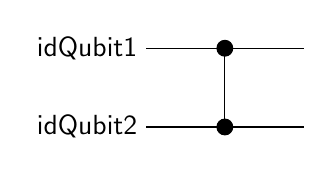
\begin{tikzpicture}[scale=.5] \node[draw=none] at (-3.5, 2) {idQubit1}; \node[draw=none] at (-3.5, 0) {idQubit2}; \draw (-2, 2) -- (2, 2); \draw[fill=black] (0, 2) circle (.2); \draw (0, 2) -- (0, 0); \draw (-2,0) -- (2, 0); \draw[fill=black] (0, 0) circle (.2); \end{tikzpicture} } \]


\begin{DoxyParams}[1]{Parameters}
\mbox{\tt in,out}  & {\em multi\+Qubit} & object representing the set of all qubits \\
\hline
\mbox{\tt in}  & {\em id\+Qubit1,id\+Qubit2} & qubits to operate upon \\
\hline
\end{DoxyParams}

\begin{DoxyExceptions}{Exceptions}
{\em exit\+With\+Error} & if {\ttfamily id\+Qubit1} or {\ttfamily id\+Qubit2} are outside \mbox{[}0, {\ttfamily multi\+Qubit.\+num\+Qubits}), or are equal \\
\hline
\end{DoxyExceptions}


Definition at line 1748 of file Qu\+E\+S\+T.\+c.



Referenced by test\+\_\+controlled\+Phase\+Gate().


\begin{DoxyCode}
1749 \{
1750     \textcolor{keywordtype}{long} \textcolor{keywordtype}{long} \textcolor{keywordtype}{int} index;
1751     \textcolor{keywordtype}{long} \textcolor{keywordtype}{long} \textcolor{keywordtype}{int} stateVecSize;
1752     \textcolor{keywordtype}{int} bit1, bit2;
1753 
1754     \textcolor{keyword}{const} \textcolor{keywordtype}{long} \textcolor{keywordtype}{long} \textcolor{keywordtype}{int} chunkSize=multiQubit.\mbox{\hyperlink{structMultiQubit_a1cad83601a78635dd278259c7ed54f18}{numAmpsPerChunk}};
1755     \textcolor{keyword}{const} \textcolor{keywordtype}{long} \textcolor{keywordtype}{long} \textcolor{keywordtype}{int} chunkId=multiQubit.\mbox{\hyperlink{structMultiQubit_ab10c88249fa3825d6227ceec01d37e37}{chunkId}};
1756 
1757     \mbox{\hyperlink{QuEST__env__local_8c_a3587b9d533e633ccf1abf9ad2ce45d8d}{QuESTAssert}}(idQubit1 >= 0 && idQubit1 < multiQubit.\mbox{\hyperlink{structMultiQubit_ab5b9795bdc6fb5855e1974dcbbaeb36f}{numQubits}}, 2, \_\_func\_\_);
1758     \mbox{\hyperlink{QuEST__env__local_8c_a3587b9d533e633ccf1abf9ad2ce45d8d}{QuESTAssert}}(idQubit2 >= 0 && idQubit2 < multiQubit.\mbox{\hyperlink{structMultiQubit_ab5b9795bdc6fb5855e1974dcbbaeb36f}{numQubits}}, 1, \_\_func\_\_);
1759     \mbox{\hyperlink{QuEST__env__local_8c_a3587b9d533e633ccf1abf9ad2ce45d8d}{QuESTAssert}}(idQubit1 != idQubit2, 3, \_\_func\_\_);
1760 
1761     \textcolor{comment}{// dimension of the state vector}
1762     stateVecSize = multiQubit.\mbox{\hyperlink{structMultiQubit_a1cad83601a78635dd278259c7ed54f18}{numAmpsPerChunk}};
1763     \mbox{\hyperlink{QuEST__precision_8h_a4b654506f18b8bfd61ad2a29a7e38c25}{REAL}} *stateVecReal = multiQubit.\mbox{\hyperlink{structMultiQubit_a45483190d6b01ef6b2f98f2bec9ab94f}{stateVec}}.\mbox{\hyperlink{structComplexArray_a4195cac6c784ea1b6271f1c7dba1548a}{real}};
1764     \mbox{\hyperlink{QuEST__precision_8h_a4b654506f18b8bfd61ad2a29a7e38c25}{REAL}} *stateVecImag = multiQubit.\mbox{\hyperlink{structMultiQubit_a45483190d6b01ef6b2f98f2bec9ab94f}{stateVec}}.\mbox{\hyperlink{structComplexArray_a79dde47c7ae530c79cebfdf57b225968}{imag}};
1765 
1766 \textcolor{preprocessor}{# ifdef \_OPENMP}
1767 \textcolor{preprocessor}{# pragma omp parallel for \(\backslash\)}
1768 \textcolor{preprocessor}{    default  (none)                          \(\backslash\)}
1769 \textcolor{preprocessor}{    shared   (stateVecSize, stateVecReal,stateVecImag ) \(\backslash\)}
1770 \textcolor{preprocessor}{    private  (index,bit1,bit2)                 \(\backslash\)}
1771 \textcolor{preprocessor}{    schedule (static)}
1772 \textcolor{preprocessor}{# endif}
1773     \textcolor{keywordflow}{for} (index=0; index<stateVecSize; index++) \{
1774         bit1 = \mbox{\hyperlink{QuEST_8c_a100463f6ec212c76a5fad99579000505}{extractBit}} (idQubit1, index+chunkId*chunkSize);
1775         bit2 = \mbox{\hyperlink{QuEST_8c_a100463f6ec212c76a5fad99579000505}{extractBit}} (idQubit2, index+chunkId*chunkSize);
1776         \textcolor{keywordflow}{if} (bit1 && bit2) \{
1777             stateVecReal [index] = - stateVecReal [index];
1778             stateVecImag [index] = - stateVecImag [index];
1779         \}
1780     \}
1781 \}
\end{DoxyCode}
\mbox{\Hypertarget{QuEST_8c_ad41f82b41149393a642391b67b3a287e}\label{QuEST_8c_ad41f82b41149393a642391b67b3a287e}} 
\index{Qu\+E\+S\+T.\+c@{Qu\+E\+S\+T.\+c}!controlled\+Rotate\+Around\+Axis@{controlled\+Rotate\+Around\+Axis}}
\index{controlled\+Rotate\+Around\+Axis@{controlled\+Rotate\+Around\+Axis}!Qu\+E\+S\+T.\+c@{Qu\+E\+S\+T.\+c}}
\paragraph{\texorpdfstring{controlled\+Rotate\+Around\+Axis()}{controlledRotateAroundAxis()}}
{\footnotesize\ttfamily void controlled\+Rotate\+Around\+Axis (\begin{DoxyParamCaption}\item[{\mbox{\hyperlink{structMultiQubit}{Multi\+Qubit}}}]{multi\+Qubit,  }\item[{const int}]{control\+Qubit,  }\item[{const int}]{target\+Qubit,  }\item[{\mbox{\hyperlink{QuEST__precision_8h_a4b654506f18b8bfd61ad2a29a7e38c25}{R\+E\+AL}}}]{angle,  }\item[{\mbox{\hyperlink{structVector}{Vector}}}]{axis }\end{DoxyParamCaption})}



Applies a controlled rotation by a given angle around a given vector on the Bloch-\/sphere. 

The vector must not be zero (else an error is thrown), but needn\textquotesingle{}t be unit magnitude.

For angle $\theta$ and axis vector $\vec{n}$, applies $R_{\hat{n}} = \exp \left(- i \frac{\theta}{2} \hat{n} \cdot \vec{\sigma} \right) $ to states where the target qubit is 1 ( $\vec{\sigma}$ is the vector of Pauli matrices).

\[ \setlength{\fboxrule}{0.01pt} \fbox{ 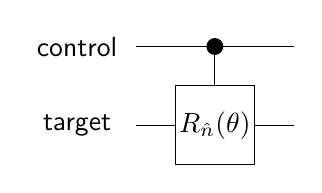
\begin{tikzpicture}[scale=.5] \node[draw=none] at (-3.5, 2) {control}; \node[draw=none] at (-3.5, 0) {target}; \draw (-2, 2) -- (2, 2); \draw[fill=black] (0, 2) circle (.2); \draw (0, 2) -- (0, 1); \draw (-2,0) -- (-1, 0); \draw (1, 0) -- (2, 0); \draw (-1,-1)--(-1,1)--(1,1)--(1,-1)--cycle; \node[draw=none] at (0, 0) {$R_{\hat{n}}(\theta)$}; \end{tikzpicture} } \]


\begin{DoxyParams}[1]{Parameters}
\mbox{\tt in,out}  & {\em multi\+Qubit} & object representing the set of all qubits \\
\hline
\mbox{\tt in}  & {\em control\+Qubit} & qubit with value 1 in the rotated states \\
\hline
\mbox{\tt in}  & {\em target\+Qubit} & qubit to rotate \\
\hline
\mbox{\tt in}  & {\em angle} & angle by which to rotate in radians \\
\hline
\mbox{\tt in}  & {\em axis} & vector around which to rotate (can be non-\/unit; will be normalised) \\
\hline
\end{DoxyParams}

\begin{DoxyExceptions}{Exceptions}
{\em exit\+With\+Error} & if either {\ttfamily control\+Qubit} or {\ttfamily target\+Qubit} are outside \mbox{[}0, {\ttfamily multi\+Qubit.\+num\+Qubits}) or are equal or if {\ttfamily axis} is the zero vector \\
\hline
\end{DoxyExceptions}


Definition at line 459 of file Qu\+E\+S\+T.\+c.



Referenced by controlled\+Rotate\+X(), controlled\+Rotate\+Y(), and controlled\+Rotate\+Z().


\begin{DoxyCode}
459                                                                                                            
                         \{
460 
461     \textcolor{keywordtype}{double} mag = sqrt(pow(axis.\mbox{\hyperlink{structVector_aac7abe171ba4bada50ed72acba6259fc}{x}},2) + pow(axis.\mbox{\hyperlink{structVector_a375ca805d4c808a53d7c4e0c737ae3de}{y}},2) + pow(axis.\mbox{\hyperlink{structVector_ad4e863651be7d6b7e2b28cd7445a0ccf}{z}},2));
462     \mbox{\hyperlink{structVector}{Vector}} unitAxis = \{axis.\mbox{\hyperlink{structVector_aac7abe171ba4bada50ed72acba6259fc}{x}}/mag, axis.\mbox{\hyperlink{structVector_a375ca805d4c808a53d7c4e0c737ae3de}{y}}/mag, axis.\mbox{\hyperlink{structVector_ad4e863651be7d6b7e2b28cd7445a0ccf}{z}}/mag\};
463 
464     \mbox{\hyperlink{structComplex}{Complex}} alpha, beta;
465     alpha.\mbox{\hyperlink{structComplex_a479ad939835457595fcca3ca55c06283}{real}} = cos(angle/2.0);
466     alpha.\mbox{\hyperlink{structComplex_a1151948284b21c0052f203f23ab931d9}{imag}} = -sin(angle/2.0)*unitAxis.\mbox{\hyperlink{structVector_ad4e863651be7d6b7e2b28cd7445a0ccf}{z}};       
467     beta.\mbox{\hyperlink{structComplex_a479ad939835457595fcca3ca55c06283}{real}} = sin(angle/2.0)*unitAxis.\mbox{\hyperlink{structVector_a375ca805d4c808a53d7c4e0c737ae3de}{y}};
468     beta.\mbox{\hyperlink{structComplex_a1151948284b21c0052f203f23ab931d9}{imag}} = -sin(angle/2.0)*unitAxis.\mbox{\hyperlink{structVector_aac7abe171ba4bada50ed72acba6259fc}{x}};
469     \mbox{\hyperlink{QuEST__env__local_8c_ab4812953bc457405b3aa05a4c2f64f4a}{controlledCompactUnitary}}(multiQubit, controlQubit, targetQubit, alpha, beta);
470 \}
\end{DoxyCode}
\mbox{\Hypertarget{QuEST_8c_ac6923ac57e67d9a21096e06f6a9012f6}\label{QuEST_8c_ac6923ac57e67d9a21096e06f6a9012f6}} 
\index{Qu\+E\+S\+T.\+c@{Qu\+E\+S\+T.\+c}!controlled\+RotateX@{controlled\+RotateX}}
\index{controlled\+RotateX@{controlled\+RotateX}!Qu\+E\+S\+T.\+c@{Qu\+E\+S\+T.\+c}}
\paragraph{\texorpdfstring{controlled\+Rotate\+X()}{controlledRotateX()}}
{\footnotesize\ttfamily void controlled\+RotateX (\begin{DoxyParamCaption}\item[{\mbox{\hyperlink{structMultiQubit}{Multi\+Qubit}}}]{multi\+Qubit,  }\item[{const int}]{control\+Qubit,  }\item[{const int}]{target\+Qubit,  }\item[{\mbox{\hyperlink{QuEST__precision_8h_a4b654506f18b8bfd61ad2a29a7e38c25}{R\+E\+AL}}}]{angle }\end{DoxyParamCaption})}



Applies a controlled rotation by a given angle around the X-\/axis of the Bloch-\/sphere. 

The target qubit is rotated in states where the control qubit has value 1.

\[ \setlength{\fboxrule}{0.01pt} \fbox{ 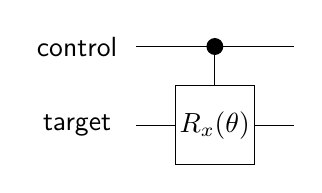
\begin{tikzpicture}[scale=.5] \node[draw=none] at (-3.5, 2) {control}; \node[draw=none] at (-3.5, 0) {target}; \draw (-2, 2) -- (2, 2); \draw[fill=black] (0, 2) circle (.2); \draw (0, 2) -- (0, 1); \draw (-2,0) -- (-1, 0); \draw (1, 0) -- (2, 0); \draw (-1,-1)--(-1,1)--(1,1)--(1,-1)--cycle; \node[draw=none] at (0, 0) {$R_x(\theta)$}; \end{tikzpicture} } \] ~\newline
 
\begin{DoxyParams}[1]{Parameters}
\mbox{\tt in,out}  & {\em multi\+Qubit} & object representing the set of all qubits \\
\hline
\mbox{\tt in}  & {\em control\+Qubit} & qubit which has value 1 in the rotated states \\
\hline
\mbox{\tt in}  & {\em tagret\+Qubit} & qubit to rotate \\
\hline
\mbox{\tt in}  & {\em angle} & angle by which to rotate the target qubit in radians \\
\hline
\end{DoxyParams}

\begin{DoxyExceptions}{Exceptions}
{\em exit\+With\+Error} & if either {\ttfamily control\+Qubit} or {\ttfamily target\+Qubit} are outside \mbox{[}0, {\ttfamily multi\+Qubit.\+num\+Qubits}) or are equal. \\
\hline
\end{DoxyExceptions}


Definition at line 472 of file Qu\+E\+S\+T.\+c.


\begin{DoxyCode}
472                                                                                                         \{
473 
474     \mbox{\hyperlink{structVector}{Vector}} unitAxis = \{1, 0, 0\};
475     \mbox{\hyperlink{QuEST_8c_ad41f82b41149393a642391b67b3a287e}{controlledRotateAroundAxis}}(multiQubit, controlQubit, targetQubit, angle, 
      unitAxis);
476 \}
\end{DoxyCode}
\mbox{\Hypertarget{QuEST_8c_a71e90a2f7292116338c062934f9d1202}\label{QuEST_8c_a71e90a2f7292116338c062934f9d1202}} 
\index{Qu\+E\+S\+T.\+c@{Qu\+E\+S\+T.\+c}!controlled\+RotateY@{controlled\+RotateY}}
\index{controlled\+RotateY@{controlled\+RotateY}!Qu\+E\+S\+T.\+c@{Qu\+E\+S\+T.\+c}}
\paragraph{\texorpdfstring{controlled\+Rotate\+Y()}{controlledRotateY()}}
{\footnotesize\ttfamily void controlled\+RotateY (\begin{DoxyParamCaption}\item[{\mbox{\hyperlink{structMultiQubit}{Multi\+Qubit}}}]{multi\+Qubit,  }\item[{const int}]{control\+Qubit,  }\item[{const int}]{target\+Qubit,  }\item[{\mbox{\hyperlink{QuEST__precision_8h_a4b654506f18b8bfd61ad2a29a7e38c25}{R\+E\+AL}}}]{angle }\end{DoxyParamCaption})}



Applies a controlled rotation by a given angle around the Y-\/axis of the Bloch-\/sphere. 

The target qubit is rotated in states where the control qubit has value 1.

\[ \setlength{\fboxrule}{0.01pt} \fbox{ 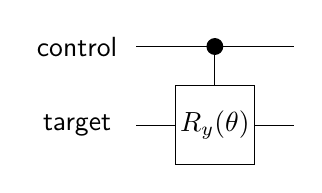
\begin{tikzpicture}[scale=.5] \node[draw=none] at (-3.5, 2) {control}; \node[draw=none] at (-3.5, 0) {target}; \draw (-2, 2) -- (2, 2); \draw[fill=black] (0, 2) circle (.2); \draw (0, 2) -- (0, 1); \draw (-2,0) -- (-1, 0); \draw (1, 0) -- (2, 0); \draw (-1,-1)--(-1,1)--(1,1)--(1,-1)--cycle; \node[draw=none] at (0, 0) {$R_y(\theta)$}; \end{tikzpicture} } \] ~\newline
 
\begin{DoxyParams}[1]{Parameters}
\mbox{\tt in,out}  & {\em multi\+Qubit} & object representing the set of all qubits \\
\hline
\mbox{\tt in}  & {\em control\+Qubit} & qubit which has value 1 in the rotated states \\
\hline
\mbox{\tt in}  & {\em tagret\+Qubit} & qubit to rotate \\
\hline
\mbox{\tt in}  & {\em angle} & angle by which to rotate the target qubit in radians \\
\hline
\end{DoxyParams}

\begin{DoxyExceptions}{Exceptions}
{\em exit\+With\+Error} & if either {\ttfamily control\+Qubit} or {\ttfamily target\+Qubit} are outside \mbox{[}0, {\ttfamily multi\+Qubit.\+num\+Qubits}) or are equal. \\
\hline
\end{DoxyExceptions}


Definition at line 478 of file Qu\+E\+S\+T.\+c.


\begin{DoxyCode}
478                                                                                                         \{
479 
480     \mbox{\hyperlink{structVector}{Vector}} unitAxis = \{0, 1, 0\};
481     \mbox{\hyperlink{QuEST_8c_ad41f82b41149393a642391b67b3a287e}{controlledRotateAroundAxis}}(multiQubit, controlQubit, targetQubit, angle, 
      unitAxis);
482 \}
\end{DoxyCode}
\mbox{\Hypertarget{QuEST_8c_a668e5d2634b02e98bc73675ccb11d61c}\label{QuEST_8c_a668e5d2634b02e98bc73675ccb11d61c}} 
\index{Qu\+E\+S\+T.\+c@{Qu\+E\+S\+T.\+c}!controlled\+RotateZ@{controlled\+RotateZ}}
\index{controlled\+RotateZ@{controlled\+RotateZ}!Qu\+E\+S\+T.\+c@{Qu\+E\+S\+T.\+c}}
\paragraph{\texorpdfstring{controlled\+Rotate\+Z()}{controlledRotateZ()}}
{\footnotesize\ttfamily void controlled\+RotateZ (\begin{DoxyParamCaption}\item[{\mbox{\hyperlink{structMultiQubit}{Multi\+Qubit}}}]{multi\+Qubit,  }\item[{const int}]{control\+Qubit,  }\item[{const int}]{target\+Qubit,  }\item[{\mbox{\hyperlink{QuEST__precision_8h_a4b654506f18b8bfd61ad2a29a7e38c25}{R\+E\+AL}}}]{angle }\end{DoxyParamCaption})}



Applies a controlled rotation by a given angle around the Z-\/axis of the Bloch-\/sphere. 

The target qubit is rotated in states where the control qubit has value 1.

\[ \setlength{\fboxrule}{0.01pt} \fbox{ 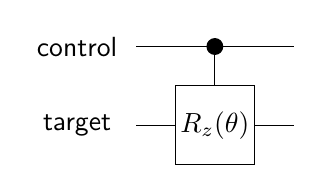
\begin{tikzpicture}[scale=.5] \node[draw=none] at (-3.5, 2) {control}; \node[draw=none] at (-3.5, 0) {target}; \draw (-2, 2) -- (2, 2); \draw[fill=black] (0, 2) circle (.2); \draw (0, 2) -- (0, 1); \draw (-2,0) -- (-1, 0); \draw (1, 0) -- (2, 0); \draw (-1,-1)--(-1,1)--(1,1)--(1,-1)--cycle; \node[draw=none] at (0, 0) {$R_z(\theta)$}; \end{tikzpicture} } \] ~\newline
 
\begin{DoxyParams}[1]{Parameters}
\mbox{\tt in,out}  & {\em multi\+Qubit} & object representing the set of all qubits \\
\hline
\mbox{\tt in}  & {\em control\+Qubit} & qubit which has value 1 in the rotated states \\
\hline
\mbox{\tt in}  & {\em tagret\+Qubit} & qubit to rotate \\
\hline
\mbox{\tt in}  & {\em angle} & angle by which to rotate the target qubit in radians \\
\hline
\end{DoxyParams}

\begin{DoxyExceptions}{Exceptions}
{\em exit\+With\+Error} & if either {\ttfamily control\+Qubit} or {\ttfamily target\+Qubit} are outside \mbox{[}0, {\ttfamily multi\+Qubit.\+num\+Qubits}) or are equal. \\
\hline
\end{DoxyExceptions}


Definition at line 484 of file Qu\+E\+S\+T.\+c.


\begin{DoxyCode}
484                                                                                                         \{
485 
486     \mbox{\hyperlink{structVector}{Vector}} unitAxis = \{0, 0, 1\};
487     \mbox{\hyperlink{QuEST_8c_ad41f82b41149393a642391b67b3a287e}{controlledRotateAroundAxis}}(multiQubit, controlQubit, targetQubit, angle, 
      unitAxis);
488 \}
\end{DoxyCode}
\mbox{\Hypertarget{QuEST_8c_a642093063a1f889f61a1311f6d6f2d3f}\label{QuEST_8c_a642093063a1f889f61a1311f6d6f2d3f}} 
\index{Qu\+E\+S\+T.\+c@{Qu\+E\+S\+T.\+c}!controlled\+Unitary\+Distributed@{controlled\+Unitary\+Distributed}}
\index{controlled\+Unitary\+Distributed@{controlled\+Unitary\+Distributed}!Qu\+E\+S\+T.\+c@{Qu\+E\+S\+T.\+c}}
\paragraph{\texorpdfstring{controlled\+Unitary\+Distributed()}{controlledUnitaryDistributed()}}
{\footnotesize\ttfamily void controlled\+Unitary\+Distributed (\begin{DoxyParamCaption}\item[{\mbox{\hyperlink{structMultiQubit}{Multi\+Qubit}}}]{multi\+Qubit,  }\item[{const int}]{control\+Qubit,  }\item[{const int}]{target\+Qubit,  }\item[{\mbox{\hyperlink{structComplex}{Complex}}}]{rot1,  }\item[{\mbox{\hyperlink{structComplex}{Complex}}}]{rot2,  }\item[{\mbox{\hyperlink{structComplexArray}{Complex\+Array}}}]{state\+Vec\+Up,  }\item[{\mbox{\hyperlink{structComplexArray}{Complex\+Array}}}]{state\+Vec\+Lo,  }\item[{\mbox{\hyperlink{structComplexArray}{Complex\+Array}}}]{state\+Vec\+Out }\end{DoxyParamCaption})}



Rotate a single qubit in the state vector of probability amplitudes, given two complex numbers alpha and beta and a subset of the state vector with upper and lower block values stored seperately. 

Only perform the rotation where the control qubit is one.


\begin{DoxyParams}[1]{Parameters}
\mbox{\tt in,out}  & {\em multi\+Qubit} & object representing the set of qubits \\
\hline
\mbox{\tt in}  & {\em target\+Qubit} & qubit to rotate \\
\hline
\mbox{\tt in}  & {\em control\+Qubit} & qubit to determine whether or not to perform a rotation \\
\hline
\mbox{\tt in}  & {\em rot1} & rotation angle \\
\hline
\mbox{\tt in}  & {\em rot2} & rotation angle \\
\hline
\mbox{\tt in}  & {\em state\+Vec\+Up} & probability amplitudes in upper half of a block \\
\hline
\mbox{\tt in}  & {\em state\+Vec\+Lo} & probability amplitudes in lower half of a block \\
\hline
\mbox{\tt out}  & {\em state\+Vec\+Out} & array section to update (will correspond to either the lower or upper half of a block) \\
\hline
\end{DoxyParams}


Definition at line 992 of file Qu\+E\+S\+T.\+c.



References Multi\+Qubit\+::chunk\+Id, extract\+Bit(), Complex\+Array\+::imag, Complex\+::imag, Multi\+Qubit\+::num\+Amps\+Per\+Chunk, Complex\+Array\+::real, R\+E\+AL, and Complex\+::real.



Referenced by controlled\+Unitary().


\begin{DoxyCode}
997 \{
998 
999     \mbox{\hyperlink{QuEST__precision_8h_a4b654506f18b8bfd61ad2a29a7e38c25}{REAL}}   stateRealUp,stateRealLo,stateImagUp,stateImagLo;
1000     \textcolor{keywordtype}{long} \textcolor{keywordtype}{long} \textcolor{keywordtype}{int} thisTask;  
1001     \textcolor{keyword}{const} \textcolor{keywordtype}{long} \textcolor{keywordtype}{long} \textcolor{keywordtype}{int} numTasks=multiQubit.\mbox{\hyperlink{structMultiQubit_a1cad83601a78635dd278259c7ed54f18}{numAmpsPerChunk}};
1002     \textcolor{keyword}{const} \textcolor{keywordtype}{long} \textcolor{keywordtype}{long} \textcolor{keywordtype}{int} chunkSize=multiQubit.\mbox{\hyperlink{structMultiQubit_a1cad83601a78635dd278259c7ed54f18}{numAmpsPerChunk}};
1003     \textcolor{keyword}{const} \textcolor{keywordtype}{long} \textcolor{keywordtype}{long} \textcolor{keywordtype}{int} chunkId=multiQubit.\mbox{\hyperlink{structMultiQubit_ab10c88249fa3825d6227ceec01d37e37}{chunkId}};
1004 
1005     \textcolor{keywordtype}{int} controlBit;
1006 
1007     \mbox{\hyperlink{QuEST__precision_8h_a4b654506f18b8bfd61ad2a29a7e38c25}{REAL}} rot1Real=rot1.\mbox{\hyperlink{structComplex_a479ad939835457595fcca3ca55c06283}{real}}, rot1Imag=rot1.\mbox{\hyperlink{structComplex_a1151948284b21c0052f203f23ab931d9}{imag}};
1008     \mbox{\hyperlink{QuEST__precision_8h_a4b654506f18b8bfd61ad2a29a7e38c25}{REAL}} rot2Real=rot2.\mbox{\hyperlink{structComplex_a479ad939835457595fcca3ca55c06283}{real}}, rot2Imag=rot2.\mbox{\hyperlink{structComplex_a1151948284b21c0052f203f23ab931d9}{imag}};
1009     \mbox{\hyperlink{QuEST__precision_8h_a4b654506f18b8bfd61ad2a29a7e38c25}{REAL}} *stateVecRealUp=stateVecUp.\mbox{\hyperlink{structComplexArray_a4195cac6c784ea1b6271f1c7dba1548a}{real}}, *stateVecImagUp=stateVecUp.
      \mbox{\hyperlink{structComplexArray_a79dde47c7ae530c79cebfdf57b225968}{imag}};
1010     \mbox{\hyperlink{QuEST__precision_8h_a4b654506f18b8bfd61ad2a29a7e38c25}{REAL}} *stateVecRealLo=stateVecLo.\mbox{\hyperlink{structComplexArray_a4195cac6c784ea1b6271f1c7dba1548a}{real}}, *stateVecImagLo=stateVecLo.
      \mbox{\hyperlink{structComplexArray_a79dde47c7ae530c79cebfdf57b225968}{imag}};
1011     \mbox{\hyperlink{QuEST__precision_8h_a4b654506f18b8bfd61ad2a29a7e38c25}{REAL}} *stateVecRealOut=stateVecOut.\mbox{\hyperlink{structComplexArray_a4195cac6c784ea1b6271f1c7dba1548a}{real}}, *stateVecImagOut=stateVecOut.
      \mbox{\hyperlink{structComplexArray_a79dde47c7ae530c79cebfdf57b225968}{imag}};
1012 
1013 \textcolor{preprocessor}{# ifdef \_OPENMP}
1014 \textcolor{preprocessor}{# pragma omp parallel \(\backslash\)}
1015 \textcolor{preprocessor}{    default  (none) \(\backslash\)}
1016 \textcolor{preprocessor}{    shared   (stateVecRealUp,stateVecImagUp,stateVecRealLo,stateVecImagLo,stateVecRealOut,stateVecImagOut, 
      \(\backslash\)}
1017 \textcolor{preprocessor}{            rot1Real,rot1Imag, rot2Real,rot2Imag) \(\backslash\)}
1018 \textcolor{preprocessor}{    private  (thisTask,stateRealUp,stateImagUp,stateRealLo,stateImagLo,controlBit)}
1019 \textcolor{preprocessor}{# endif}
1020     \{
1021 \textcolor{preprocessor}{# ifdef \_OPENMP}
1022 \textcolor{preprocessor}{# pragma omp for schedule (static)}
1023 \textcolor{preprocessor}{# endif}
1024         \textcolor{keywordflow}{for} (thisTask=0; thisTask<numTasks; thisTask++) \{
1025             controlBit = \mbox{\hyperlink{QuEST_8c_a100463f6ec212c76a5fad99579000505}{extractBit}} (controlQubit, thisTask+chunkId*chunkSize);
1026             \textcolor{keywordflow}{if} (controlBit)\{
1027                 \textcolor{comment}{// store current state vector values in temp variables}
1028                 stateRealUp = stateVecRealUp[thisTask];
1029                 stateImagUp = stateVecImagUp[thisTask];
1030 
1031                 stateRealLo = stateVecRealLo[thisTask];
1032                 stateImagLo = stateVecImagLo[thisTask];
1033 
1034                 stateVecRealOut[thisTask] = rot1Real*stateRealUp - rot1Imag*stateImagUp 
1035                     + rot2Real*stateRealLo - rot2Imag*stateImagLo;
1036                 stateVecImagOut[thisTask] = rot1Real*stateImagUp + rot1Imag*stateRealUp 
1037                     + rot2Real*stateImagLo + rot2Imag*stateRealLo;
1038             \}
1039         \}
1040     \}
1041 \}
\end{DoxyCode}
\mbox{\Hypertarget{QuEST_8c_a8a4afcff70195a306c082b8ed8d4e09a}\label{QuEST_8c_a8a4afcff70195a306c082b8ed8d4e09a}} 
\index{Qu\+E\+S\+T.\+c@{Qu\+E\+S\+T.\+c}!controlled\+Unitary\+Local@{controlled\+Unitary\+Local}}
\index{controlled\+Unitary\+Local@{controlled\+Unitary\+Local}!Qu\+E\+S\+T.\+c@{Qu\+E\+S\+T.\+c}}
\paragraph{\texorpdfstring{controlled\+Unitary\+Local()}{controlledUnitaryLocal()}}
{\footnotesize\ttfamily void controlled\+Unitary\+Local (\begin{DoxyParamCaption}\item[{\mbox{\hyperlink{structMultiQubit}{Multi\+Qubit}}}]{multi\+Qubit,  }\item[{const int}]{control\+Qubit,  }\item[{const int}]{target\+Qubit,  }\item[{\mbox{\hyperlink{structComplexMatrix2}{Complex\+Matrix2}}}]{u }\end{DoxyParamCaption})}



Definition at line 850 of file Qu\+E\+S\+T.\+c.



References Multi\+Qubit\+::chunk\+Id, extract\+Bit(), Complex\+Array\+::imag, Complex\+::imag, Multi\+Qubit\+::num\+Amps\+Per\+Chunk, Complex\+Matrix2\+::r0c0, Complex\+Matrix2\+::r0c1, Complex\+Matrix2\+::r1c0, Complex\+Matrix2\+::r1c1, Complex\+Array\+::real, R\+E\+AL, Complex\+::real, and Multi\+Qubit\+::state\+Vec.



Referenced by controlled\+Unitary().


\begin{DoxyCode}
852 \{
853     \textcolor{keywordtype}{long} \textcolor{keywordtype}{long} \textcolor{keywordtype}{int} sizeBlock, sizeHalfBlock;
854     \textcolor{keywordtype}{long} \textcolor{keywordtype}{long} \textcolor{keywordtype}{int} thisBlock, \textcolor{comment}{// current block}
855          indexUp,indexLo;    \textcolor{comment}{// current index and corresponding index in lower half block}
856 
857     \mbox{\hyperlink{QuEST__precision_8h_a4b654506f18b8bfd61ad2a29a7e38c25}{REAL}} stateRealUp,stateRealLo,stateImagUp,stateImagLo;
858     \textcolor{keywordtype}{long} \textcolor{keywordtype}{long} \textcolor{keywordtype}{int} thisTask;         
859     \textcolor{keyword}{const} \textcolor{keywordtype}{long} \textcolor{keywordtype}{long} \textcolor{keywordtype}{int} numTasks=multiQubit.\mbox{\hyperlink{structMultiQubit_a1cad83601a78635dd278259c7ed54f18}{numAmpsPerChunk}}>>1;
860     \textcolor{keyword}{const} \textcolor{keywordtype}{long} \textcolor{keywordtype}{long} \textcolor{keywordtype}{int} chunkSize=multiQubit.\mbox{\hyperlink{structMultiQubit_a1cad83601a78635dd278259c7ed54f18}{numAmpsPerChunk}};
861     \textcolor{keyword}{const} \textcolor{keywordtype}{long} \textcolor{keywordtype}{long} \textcolor{keywordtype}{int} chunkId=multiQubit.\mbox{\hyperlink{structMultiQubit_ab10c88249fa3825d6227ceec01d37e37}{chunkId}};
862 
863     \textcolor{keywordtype}{int} controlBit;
864 
865     \textcolor{comment}{// set dimensions}
866     sizeHalfBlock = 1LL << targetQubit;  
867     sizeBlock     = 2LL * sizeHalfBlock; 
868 
869     \textcolor{comment}{// Can't use multiQubit.stateVec as a private OMP var}
870     \mbox{\hyperlink{QuEST__precision_8h_a4b654506f18b8bfd61ad2a29a7e38c25}{REAL}} *stateVecReal = multiQubit.\mbox{\hyperlink{structMultiQubit_a45483190d6b01ef6b2f98f2bec9ab94f}{stateVec}}.\mbox{\hyperlink{structComplexArray_a4195cac6c784ea1b6271f1c7dba1548a}{real}};
871     \mbox{\hyperlink{QuEST__precision_8h_a4b654506f18b8bfd61ad2a29a7e38c25}{REAL}} *stateVecImag = multiQubit.\mbox{\hyperlink{structMultiQubit_a45483190d6b01ef6b2f98f2bec9ab94f}{stateVec}}.\mbox{\hyperlink{structComplexArray_a79dde47c7ae530c79cebfdf57b225968}{imag}};
872 
873 \textcolor{preprocessor}{# ifdef \_OPENMP}
874 \textcolor{preprocessor}{# pragma omp parallel \(\backslash\)}
875 \textcolor{preprocessor}{    default  (none) \(\backslash\)}
876 \textcolor{preprocessor}{    shared   (sizeBlock,sizeHalfBlock, stateVecReal,stateVecImag, u) \(\backslash\)}
877 \textcolor{preprocessor}{    private  (thisTask,thisBlock ,indexUp,indexLo,
       stateRealUp,stateImagUp,stateRealLo,stateImagLo,controlBit) }
878 \textcolor{preprocessor}{# endif}
879     \{
880 \textcolor{preprocessor}{# ifdef \_OPENMP}
881 \textcolor{preprocessor}{# pragma omp for schedule (static)}
882 \textcolor{preprocessor}{# endif}
883         \textcolor{keywordflow}{for} (thisTask=0; thisTask<numTasks; thisTask++) \{
884 
885             thisBlock   = thisTask / sizeHalfBlock;
886             indexUp     = thisBlock*sizeBlock + thisTask%sizeHalfBlock;
887             indexLo     = indexUp + sizeHalfBlock;
888 
889             controlBit = \mbox{\hyperlink{QuEST_8c_a100463f6ec212c76a5fad99579000505}{extractBit}} (controlQubit, indexUp+chunkId*chunkSize);
890             \textcolor{keywordflow}{if} (controlBit)\{
891                 \textcolor{comment}{// store current state vector values in temp variables}
892                 stateRealUp = stateVecReal[indexUp];
893                 stateImagUp = stateVecImag[indexUp];
894 
895                 stateRealLo = stateVecReal[indexLo];
896                 stateImagLo = stateVecImag[indexLo];
897 
898 
899                 \textcolor{comment}{// state[indexUp] = u00 * state[indexUp] + u01 * state[indexLo]}
900                 stateVecReal[indexUp] = u.\mbox{\hyperlink{structComplexMatrix2_ae72b4458233b077a636beee1892e81ff}{r0c0}}.\mbox{\hyperlink{structComplex_a479ad939835457595fcca3ca55c06283}{real}}*stateRealUp - u.\mbox{\hyperlink{structComplexMatrix2_ae72b4458233b077a636beee1892e81ff}{r0c0}}.
      \mbox{\hyperlink{structComplex_a1151948284b21c0052f203f23ab931d9}{imag}}*stateImagUp 
901                     + u.\mbox{\hyperlink{structComplexMatrix2_a0f3932f055a8b05cef361bce25d51172}{r0c1}}.\mbox{\hyperlink{structComplex_a479ad939835457595fcca3ca55c06283}{real}}*stateRealLo - u.\mbox{\hyperlink{structComplexMatrix2_a0f3932f055a8b05cef361bce25d51172}{r0c1}}.\mbox{\hyperlink{structComplex_a1151948284b21c0052f203f23ab931d9}{imag}}*stateImagLo;
902                 stateVecImag[indexUp] = u.\mbox{\hyperlink{structComplexMatrix2_ae72b4458233b077a636beee1892e81ff}{r0c0}}.\mbox{\hyperlink{structComplex_a479ad939835457595fcca3ca55c06283}{real}}*stateImagUp + u.\mbox{\hyperlink{structComplexMatrix2_ae72b4458233b077a636beee1892e81ff}{r0c0}}.
      \mbox{\hyperlink{structComplex_a1151948284b21c0052f203f23ab931d9}{imag}}*stateRealUp 
903                     + u.\mbox{\hyperlink{structComplexMatrix2_a0f3932f055a8b05cef361bce25d51172}{r0c1}}.\mbox{\hyperlink{structComplex_a479ad939835457595fcca3ca55c06283}{real}}*stateImagLo + u.\mbox{\hyperlink{structComplexMatrix2_a0f3932f055a8b05cef361bce25d51172}{r0c1}}.\mbox{\hyperlink{structComplex_a1151948284b21c0052f203f23ab931d9}{imag}}*stateRealLo;
904 
905                 \textcolor{comment}{// state[indexLo] = u10  * state[indexUp] + u11 * state[indexLo]}
906                 stateVecReal[indexLo] = u.\mbox{\hyperlink{structComplexMatrix2_ab98282015ed2065e53fbc9638e2583ab}{r1c0}}.\mbox{\hyperlink{structComplex_a479ad939835457595fcca3ca55c06283}{real}}*stateRealUp  - u.
      \mbox{\hyperlink{structComplexMatrix2_ab98282015ed2065e53fbc9638e2583ab}{r1c0}}.\mbox{\hyperlink{structComplex_a1151948284b21c0052f203f23ab931d9}{imag}}*stateImagUp 
907                     + u.\mbox{\hyperlink{structComplexMatrix2_a763007c3070802373549ba0350f83c8a}{r1c1}}.\mbox{\hyperlink{structComplex_a479ad939835457595fcca3ca55c06283}{real}}*stateRealLo  -  u.\mbox{\hyperlink{structComplexMatrix2_a763007c3070802373549ba0350f83c8a}{r1c1}}.\mbox{\hyperlink{structComplex_a1151948284b21c0052f203f23ab931d9}{imag}}*stateImagLo;
908                 stateVecImag[indexLo] = u.\mbox{\hyperlink{structComplexMatrix2_ab98282015ed2065e53fbc9638e2583ab}{r1c0}}.\mbox{\hyperlink{structComplex_a479ad939835457595fcca3ca55c06283}{real}}*stateImagUp + u.\mbox{\hyperlink{structComplexMatrix2_ab98282015ed2065e53fbc9638e2583ab}{r1c0}}.
      \mbox{\hyperlink{structComplex_a1151948284b21c0052f203f23ab931d9}{imag}}*stateRealUp 
909                     + u.\mbox{\hyperlink{structComplexMatrix2_a763007c3070802373549ba0350f83c8a}{r1c1}}.\mbox{\hyperlink{structComplex_a479ad939835457595fcca3ca55c06283}{real}}*stateImagLo + u.\mbox{\hyperlink{structComplexMatrix2_a763007c3070802373549ba0350f83c8a}{r1c1}}.\mbox{\hyperlink{structComplex_a1151948284b21c0052f203f23ab931d9}{imag}}*stateRealLo;
910             \}
911         \} 
912     \}
913 
914 \}
\end{DoxyCode}
\mbox{\Hypertarget{QuEST_8c_a9c02591bc64c2918503afa231d90d83f}\label{QuEST_8c_a9c02591bc64c2918503afa231d90d83f}} 
\index{Qu\+E\+S\+T.\+c@{Qu\+E\+S\+T.\+c}!create\+Multi\+Qubit@{create\+Multi\+Qubit}}
\index{create\+Multi\+Qubit@{create\+Multi\+Qubit}!Qu\+E\+S\+T.\+c@{Qu\+E\+S\+T.\+c}}
\paragraph{\texorpdfstring{create\+Multi\+Qubit()}{createMultiQubit()}}
{\footnotesize\ttfamily void create\+Multi\+Qubit (\begin{DoxyParamCaption}\item[{\mbox{\hyperlink{structMultiQubit}{Multi\+Qubit}} $\ast$}]{multi\+Qubit,  }\item[{int}]{num\+Qubits,  }\item[{\mbox{\hyperlink{structQuESTEnv}{Qu\+E\+S\+T\+Env}}}]{env }\end{DoxyParamCaption})}



Create a \mbox{\hyperlink{structMultiQubit}{Multi\+Qubit}} object representing a set of qubits. 

Allocate space for state vector of probability amplitudes, including space for temporary values to be copied from one other chunk if running the distributed version. Define properties related to the size of the set of qubits. init\+State\+Zero should be called after this to initialise the qubits to the zero state.


\begin{DoxyParams}[1]{Parameters}
\mbox{\tt in,out}  & {\em multi\+Qubit} & a pointer to an object representing the set of qubits \\
\hline
\mbox{\tt in}  & {\em num\+Qubits} & number of qubits in the system \\
\hline
\mbox{\tt in}  & {\em env} & object representing the execution environment (local, multinode etc) \\
\hline
\end{DoxyParams}

\begin{DoxyExceptions}{Exceptions}
{\em exit\+With\+Error} & if {\ttfamily num\+Qubits} $<$= 0 \\
\hline
\end{DoxyExceptions}


Definition at line 44 of file Qu\+E\+S\+T.\+c.



Referenced by main(), test\+\_\+collapse\+To\+Outcome(), test\+\_\+compact\+Unitary(), test\+\_\+controlled\+Compact\+Unitary(), test\+\_\+controlled\+Not(), test\+\_\+controlled\+Phase\+Gate(), test\+\_\+controlled\+Unitary(), test\+\_\+find\+Probability\+Of\+Outcome(), test\+\_\+get\+Imag\+Amp\+El(), test\+\_\+get\+Prob\+El(), test\+\_\+get\+Real\+Amp\+El(), test\+\_\+hadamard(), test\+\_\+init\+Classical\+State(), test\+\_\+init\+State\+Plus(), test\+\_\+init\+State\+Zero(), test\+\_\+measure(), test\+\_\+measure\+With\+Stats(), test\+\_\+multi\+Controlled\+Phase\+Gate(), test\+\_\+multi\+Controlled\+Unitary(), test\+\_\+s\+Gate(), test\+\_\+sigma\+X(), test\+\_\+sigma\+Y(), test\+\_\+sigma\+Z(), test\+\_\+t\+Gate(), and test\+\_\+unitary().


\begin{DoxyCode}
45 \{
46     \mbox{\hyperlink{QuEST__env__local_8c_a3587b9d533e633ccf1abf9ad2ce45d8d}{QuESTAssert}}(numQubits>0, 9, \_\_func\_\_);
47     \textcolor{keywordtype}{long} \textcolor{keywordtype}{long} \textcolor{keywordtype}{int} numAmps = 1L << numQubits;
48     \textcolor{keywordtype}{long} \textcolor{keywordtype}{long} \textcolor{keywordtype}{int} numAmpsPerRank = numAmps/\mbox{\hyperlink{runTests_8c_a5fd8ba97fcae3408ae6221dfc3cc1f93}{env}}.\mbox{\hyperlink{structQuESTEnv_af22aacd7c9905accae28484785c193b4}{numRanks}};
49 
50     multiQubit->\mbox{\hyperlink{structMultiQubit_a45483190d6b01ef6b2f98f2bec9ab94f}{stateVec}}.\mbox{\hyperlink{structComplexArray_a4195cac6c784ea1b6271f1c7dba1548a}{real}} = malloc(numAmpsPerRank * \textcolor{keyword}{sizeof}(*(multiQubit->
      \mbox{\hyperlink{structMultiQubit_a45483190d6b01ef6b2f98f2bec9ab94f}{stateVec}}.\mbox{\hyperlink{structComplexArray_a4195cac6c784ea1b6271f1c7dba1548a}{real}})));
51     multiQubit->\mbox{\hyperlink{structMultiQubit_a45483190d6b01ef6b2f98f2bec9ab94f}{stateVec}}.\mbox{\hyperlink{structComplexArray_a79dde47c7ae530c79cebfdf57b225968}{imag}} = malloc(numAmpsPerRank * \textcolor{keyword}{sizeof}(*(multiQubit->
      \mbox{\hyperlink{structMultiQubit_a45483190d6b01ef6b2f98f2bec9ab94f}{stateVec}}.\mbox{\hyperlink{structComplexArray_a79dde47c7ae530c79cebfdf57b225968}{imag}})));
52     \textcolor{keywordflow}{if} (\mbox{\hyperlink{runTests_8c_a5fd8ba97fcae3408ae6221dfc3cc1f93}{env}}.\mbox{\hyperlink{structQuESTEnv_af22aacd7c9905accae28484785c193b4}{numRanks}}>1)\{
53         multiQubit->\mbox{\hyperlink{structMultiQubit_a76f7db4eab52d2b30f58f973ada809c5}{pairStateVec}}.\mbox{\hyperlink{structComplexArray_a4195cac6c784ea1b6271f1c7dba1548a}{real}} = malloc(numAmpsPerRank * \textcolor{keyword}{sizeof}(*(multiQubit->
      \mbox{\hyperlink{structMultiQubit_a76f7db4eab52d2b30f58f973ada809c5}{pairStateVec}}.\mbox{\hyperlink{structComplexArray_a4195cac6c784ea1b6271f1c7dba1548a}{real}})));
54         multiQubit->\mbox{\hyperlink{structMultiQubit_a76f7db4eab52d2b30f58f973ada809c5}{pairStateVec}}.\mbox{\hyperlink{structComplexArray_a79dde47c7ae530c79cebfdf57b225968}{imag}} = malloc(numAmpsPerRank * \textcolor{keyword}{sizeof}(*(multiQubit->
      \mbox{\hyperlink{structMultiQubit_a76f7db4eab52d2b30f58f973ada809c5}{pairStateVec}}.\mbox{\hyperlink{structComplexArray_a79dde47c7ae530c79cebfdf57b225968}{imag}})));
55     \}
56 
57     \textcolor{keywordflow}{if} ( (!(multiQubit->\mbox{\hyperlink{structMultiQubit_a45483190d6b01ef6b2f98f2bec9ab94f}{stateVec}}.\mbox{\hyperlink{structComplexArray_a4195cac6c784ea1b6271f1c7dba1548a}{real}}) || !(multiQubit->\mbox{\hyperlink{structMultiQubit_a45483190d6b01ef6b2f98f2bec9ab94f}{stateVec}}.
      \mbox{\hyperlink{structComplexArray_a79dde47c7ae530c79cebfdf57b225968}{imag}}))
58             && numAmpsPerRank ) \{
59         printf(\textcolor{stringliteral}{"Could not allocate memory!"});
60         exit (EXIT\_FAILURE);
61     \}
62 
63     \textcolor{keywordflow}{if} ( \mbox{\hyperlink{runTests_8c_a5fd8ba97fcae3408ae6221dfc3cc1f93}{env}}.\mbox{\hyperlink{structQuESTEnv_af22aacd7c9905accae28484785c193b4}{numRanks}}>1 && (!(multiQubit->\mbox{\hyperlink{structMultiQubit_a76f7db4eab52d2b30f58f973ada809c5}{pairStateVec}}.
      \mbox{\hyperlink{structComplexArray_a4195cac6c784ea1b6271f1c7dba1548a}{real}}) || !(multiQubit->\mbox{\hyperlink{structMultiQubit_a76f7db4eab52d2b30f58f973ada809c5}{pairStateVec}}.\mbox{\hyperlink{structComplexArray_a79dde47c7ae530c79cebfdf57b225968}{imag}}))
64             && numAmpsPerRank ) \{
65         printf(\textcolor{stringliteral}{"Could not allocate memory!"});
66         exit (EXIT\_FAILURE);
67     \}
68 
69     multiQubit->\mbox{\hyperlink{structMultiQubit_ab5b9795bdc6fb5855e1974dcbbaeb36f}{numQubits}} = numQubits;
70     multiQubit->\mbox{\hyperlink{structMultiQubit_a1cad83601a78635dd278259c7ed54f18}{numAmpsPerChunk}} = numAmpsPerRank;
71     multiQubit->\mbox{\hyperlink{structMultiQubit_ab10c88249fa3825d6227ceec01d37e37}{chunkId}} = \mbox{\hyperlink{runTests_8c_a5fd8ba97fcae3408ae6221dfc3cc1f93}{env}}.\mbox{\hyperlink{structQuESTEnv_aa648bb336cf8598467cb62db00b9cee8}{rank}};
72     multiQubit->\mbox{\hyperlink{structMultiQubit_acd43f2f57991709c9e94f73662c972b2}{numChunks}} = \mbox{\hyperlink{runTests_8c_a5fd8ba97fcae3408ae6221dfc3cc1f93}{env}}.\mbox{\hyperlink{structQuESTEnv_af22aacd7c9905accae28484785c193b4}{numRanks}};
73 
74 \}
\end{DoxyCode}
\mbox{\Hypertarget{QuEST_8c_ae5d6acc322314d7a3d8a2eccf00d3b19}\label{QuEST_8c_ae5d6acc322314d7a3d8a2eccf00d3b19}} 
\index{Qu\+E\+S\+T.\+c@{Qu\+E\+S\+T.\+c}!destroy\+Multi\+Qubit@{destroy\+Multi\+Qubit}}
\index{destroy\+Multi\+Qubit@{destroy\+Multi\+Qubit}!Qu\+E\+S\+T.\+c@{Qu\+E\+S\+T.\+c}}
\paragraph{\texorpdfstring{destroy\+Multi\+Qubit()}{destroyMultiQubit()}}
{\footnotesize\ttfamily void destroy\+Multi\+Qubit (\begin{DoxyParamCaption}\item[{\mbox{\hyperlink{structMultiQubit}{Multi\+Qubit}}}]{multi\+Qubit,  }\item[{\mbox{\hyperlink{structQuESTEnv}{Qu\+E\+S\+T\+Env}}}]{env }\end{DoxyParamCaption})}



Deallocate a \mbox{\hyperlink{structMultiQubit}{Multi\+Qubit}} object representing a set of qubits. 

Free memory allocated to state vector of probability amplitudes, including temporary vector for values copied from another chunk if running the distributed version.


\begin{DoxyParams}[1]{Parameters}
\mbox{\tt in,out}  & {\em multi\+Qubit} & object to be deallocated \\
\hline
\mbox{\tt in}  & {\em env} & object representing the execution environment (local, multinode etc) \\
\hline
\end{DoxyParams}


Definition at line 76 of file Qu\+E\+S\+T.\+c.



Referenced by main(), test\+\_\+collapse\+To\+Outcome(), test\+\_\+compact\+Unitary(), test\+\_\+controlled\+Compact\+Unitary(), test\+\_\+controlled\+Not(), test\+\_\+controlled\+Phase\+Gate(), test\+\_\+controlled\+Unitary(), test\+\_\+find\+Probability\+Of\+Outcome(), test\+\_\+get\+Imag\+Amp\+El(), test\+\_\+get\+Prob\+El(), test\+\_\+get\+Real\+Amp\+El(), test\+\_\+hadamard(), test\+\_\+init\+Classical\+State(), test\+\_\+init\+State\+Plus(), test\+\_\+init\+State\+Zero(), test\+\_\+measure(), test\+\_\+measure\+With\+Stats(), test\+\_\+multi\+Controlled\+Phase\+Gate(), test\+\_\+multi\+Controlled\+Unitary(), test\+\_\+s\+Gate(), test\+\_\+sigma\+X(), test\+\_\+sigma\+Y(), test\+\_\+sigma\+Z(), test\+\_\+t\+Gate(), and test\+\_\+unitary().


\begin{DoxyCode}
76                                                            \{
77     free(multiQubit.\mbox{\hyperlink{structMultiQubit_a45483190d6b01ef6b2f98f2bec9ab94f}{stateVec}}.\mbox{\hyperlink{structComplexArray_a4195cac6c784ea1b6271f1c7dba1548a}{real}});
78     free(multiQubit.\mbox{\hyperlink{structMultiQubit_a45483190d6b01ef6b2f98f2bec9ab94f}{stateVec}}.\mbox{\hyperlink{structComplexArray_a79dde47c7ae530c79cebfdf57b225968}{imag}});
79     \textcolor{keywordflow}{if} (\mbox{\hyperlink{runTests_8c_a5fd8ba97fcae3408ae6221dfc3cc1f93}{env}}.\mbox{\hyperlink{structQuESTEnv_af22aacd7c9905accae28484785c193b4}{numRanks}}>1)\{
80         free(multiQubit.\mbox{\hyperlink{structMultiQubit_a76f7db4eab52d2b30f58f973ada809c5}{pairStateVec}}.\mbox{\hyperlink{structComplexArray_a4195cac6c784ea1b6271f1c7dba1548a}{real}});
81         free(multiQubit.\mbox{\hyperlink{structMultiQubit_a76f7db4eab52d2b30f58f973ada809c5}{pairStateVec}}.\mbox{\hyperlink{structComplexArray_a79dde47c7ae530c79cebfdf57b225968}{imag}});
82     \}
83 \}
\end{DoxyCode}
\mbox{\Hypertarget{QuEST_8c_a100463f6ec212c76a5fad99579000505}\label{QuEST_8c_a100463f6ec212c76a5fad99579000505}} 
\index{Qu\+E\+S\+T.\+c@{Qu\+E\+S\+T.\+c}!extract\+Bit@{extract\+Bit}}
\index{extract\+Bit@{extract\+Bit}!Qu\+E\+S\+T.\+c@{Qu\+E\+S\+T.\+c}}
\paragraph{\texorpdfstring{extract\+Bit()}{extractBit()}}
{\footnotesize\ttfamily static int extract\+Bit (\begin{DoxyParamCaption}\item[{const int}]{location\+Of\+Bit\+From\+Right,  }\item[{const long long int}]{the\+Encoded\+Number }\end{DoxyParamCaption})\hspace{0.3cm}{\ttfamily [static]}}



Get the value of the bit at a particular index in a number. 

S\+CB edit\+: new definition of extract\+Bit is much faster $\ast$$\ast$$\ast$ 
\begin{DoxyParams}[1]{Parameters}
\mbox{\tt in}  & {\em location\+Of\+Bit\+From\+Right} & location of bit in the\+Encoded\+Number \\
\hline
\mbox{\tt in}  & {\em the\+Encoded\+Number} & number to search \\
\hline
\end{DoxyParams}
\begin{DoxyReturn}{Returns}
the value of the bit in the\+Encoded\+Number 
\end{DoxyReturn}


Definition at line 1743 of file Qu\+E\+S\+T.\+c.



Referenced by controlled\+Compact\+Unitary\+Distributed(), controlled\+Compact\+Unitary\+Local(), controlled\+Not\+Distributed(), controlled\+Not\+Local(), controlled\+Phase\+Gate(), controlled\+Unitary\+Distributed(), controlled\+Unitary\+Local(), and init\+State\+Of\+Single\+Qubit().


\begin{DoxyCode}
1744 \{
1745     \textcolor{keywordflow}{return} (theEncodedNumber & ( 1LL << locationOfBitFromRight )) >> locationOfBitFromRight;
1746 \}
\end{DoxyCode}
\mbox{\Hypertarget{QuEST_8c_a9ac9bb717a889f09d307eda9f0b65957}\label{QuEST_8c_a9ac9bb717a889f09d307eda9f0b65957}} 
\index{Qu\+E\+S\+T.\+c@{Qu\+E\+S\+T.\+c}!find\+Probability\+Of\+Zero\+Distributed@{find\+Probability\+Of\+Zero\+Distributed}}
\index{find\+Probability\+Of\+Zero\+Distributed@{find\+Probability\+Of\+Zero\+Distributed}!Qu\+E\+S\+T.\+c@{Qu\+E\+S\+T.\+c}}
\paragraph{\texorpdfstring{find\+Probability\+Of\+Zero\+Distributed()}{findProbabilityOfZeroDistributed()}}
{\footnotesize\ttfamily \mbox{\hyperlink{QuEST__precision_8h_a4b654506f18b8bfd61ad2a29a7e38c25}{R\+E\+AL}} find\+Probability\+Of\+Zero\+Distributed (\begin{DoxyParamCaption}\item[{\mbox{\hyperlink{structMultiQubit}{Multi\+Qubit}}}]{multi\+Qubit,  }\item[{const int}]{measure\+Qubit }\end{DoxyParamCaption})}



Measure the probability of a specified qubit being in the zero state across all amplitudes held in this chunk. 

Size of regions to skip is a multiple of chunk\+Size.


\begin{DoxyParams}[1]{Parameters}
\mbox{\tt in}  & {\em multi\+Qubit} & object representing the set of qubits \\
\hline
\mbox{\tt in}  & {\em measure\+Qubit} & qubit to measure \\
\hline
\end{DoxyParams}
\begin{DoxyReturn}{Returns}
probability of qubit measure\+Qubit being zero 
\end{DoxyReturn}


Definition at line 1699 of file Qu\+E\+S\+T.\+c.



References Complex\+Array\+::imag, Multi\+Qubit\+::num\+Amps\+Per\+Chunk, Complex\+Array\+::real, R\+E\+AL, and Multi\+Qubit\+::state\+Vec.



Referenced by find\+Probability\+Of\+Outcome().


\begin{DoxyCode}
1701 \{
1702     \textcolor{comment}{// ----- measured probability}
1703     \mbox{\hyperlink{QuEST__precision_8h_a4b654506f18b8bfd61ad2a29a7e38c25}{REAL}}   totalProbability;                                  \textcolor{comment}{// probability (returned) value}
1704     \textcolor{comment}{// ----- temp variables}
1705     \textcolor{keywordtype}{long} \textcolor{keywordtype}{long} \textcolor{keywordtype}{int} thisTask;                                   \textcolor{comment}{// task based approach for expose loop with
       small granularity}
1706     \textcolor{keywordtype}{long} \textcolor{keywordtype}{long} \textcolor{keywordtype}{int} numTasks=multiQubit.\mbox{\hyperlink{structMultiQubit_a1cad83601a78635dd278259c7ed54f18}{numAmpsPerChunk}};
1707 
1708     \textcolor{comment}{// ---------------------------------------------------------------- //}
1709     \textcolor{comment}{//            find probability                                      //}
1710     \textcolor{comment}{// ---------------------------------------------------------------- //}
1711 
1712     \textcolor{comment}{// initialise returned value}
1713     totalProbability = 0.0;
1714 
1715     \mbox{\hyperlink{QuEST__precision_8h_a4b654506f18b8bfd61ad2a29a7e38c25}{REAL}} *stateVecReal = multiQubit.\mbox{\hyperlink{structMultiQubit_a45483190d6b01ef6b2f98f2bec9ab94f}{stateVec}}.\mbox{\hyperlink{structComplexArray_a4195cac6c784ea1b6271f1c7dba1548a}{real}};
1716     \mbox{\hyperlink{QuEST__precision_8h_a4b654506f18b8bfd61ad2a29a7e38c25}{REAL}} *stateVecImag = multiQubit.\mbox{\hyperlink{structMultiQubit_a45483190d6b01ef6b2f98f2bec9ab94f}{stateVec}}.\mbox{\hyperlink{structComplexArray_a79dde47c7ae530c79cebfdf57b225968}{imag}};
1717 
1718 \textcolor{preprocessor}{# ifdef \_OPENMP}
1719 \textcolor{preprocessor}{# pragma omp parallel \(\backslash\)}
1720 \textcolor{preprocessor}{    shared    (numTasks,stateVecReal,stateVecImag) \(\backslash\)}
1721 \textcolor{preprocessor}{    private   (thisTask) \(\backslash\)}
1722 \textcolor{preprocessor}{    reduction ( +:totalProbability )}
1723 \textcolor{preprocessor}{# endif}
1724     \{
1725 \textcolor{preprocessor}{# ifdef \_OPENMP}
1726 \textcolor{preprocessor}{# pragma omp for schedule  (static)}
1727 \textcolor{preprocessor}{# endif}
1728         \textcolor{keywordflow}{for} (thisTask=0; thisTask<numTasks; thisTask++) \{
1729             totalProbability += stateVecReal[thisTask]*stateVecReal[thisTask]
1730                 + stateVecImag[thisTask]*stateVecImag[thisTask];
1731         \}
1732     \}
1733 
1734     \textcolor{keywordflow}{return} totalProbability;
1735 \}
\end{DoxyCode}
\mbox{\Hypertarget{QuEST_8c_a7c02cd0e1b4eac19771a0525f023249e}\label{QuEST_8c_a7c02cd0e1b4eac19771a0525f023249e}} 
\index{Qu\+E\+S\+T.\+c@{Qu\+E\+S\+T.\+c}!find\+Probability\+Of\+Zero\+Local@{find\+Probability\+Of\+Zero\+Local}}
\index{find\+Probability\+Of\+Zero\+Local@{find\+Probability\+Of\+Zero\+Local}!Qu\+E\+S\+T.\+c@{Qu\+E\+S\+T.\+c}}
\paragraph{\texorpdfstring{find\+Probability\+Of\+Zero\+Local()}{findProbabilityOfZeroLocal()}}
{\footnotesize\ttfamily \mbox{\hyperlink{QuEST__precision_8h_a4b654506f18b8bfd61ad2a29a7e38c25}{R\+E\+AL}} find\+Probability\+Of\+Zero\+Local (\begin{DoxyParamCaption}\item[{\mbox{\hyperlink{structMultiQubit}{Multi\+Qubit}}}]{multi\+Qubit,  }\item[{const int}]{measure\+Qubit }\end{DoxyParamCaption})}



Measure the total probability of a specified qubit being in the zero state across all amplitudes in this chunk. 

Size of regions to skip is less than the size of one chunk. ~\newline
 
\begin{DoxyParams}[1]{Parameters}
\mbox{\tt in}  & {\em multi\+Qubit} & object representing the set of qubits \\
\hline
\mbox{\tt in}  & {\em measure\+Qubit} & qubit to measure \\
\hline
\end{DoxyParams}
\begin{DoxyReturn}{Returns}
probability of qubit measure\+Qubit being zero 
\end{DoxyReturn}


Definition at line 1643 of file Qu\+E\+S\+T.\+c.



References Complex\+Array\+::imag, Multi\+Qubit\+::num\+Amps\+Per\+Chunk, Complex\+Array\+::real, R\+E\+AL, and Multi\+Qubit\+::state\+Vec.



Referenced by find\+Probability\+Of\+Outcome().


\begin{DoxyCode}
1645 \{
1646     \textcolor{comment}{// ----- sizes}
1647     \textcolor{keywordtype}{long} \textcolor{keywordtype}{long} \textcolor{keywordtype}{int} sizeBlock,                                  \textcolor{comment}{// size of blocks}
1648          sizeHalfBlock;                                       \textcolor{comment}{// size of blocks halved}
1649     \textcolor{comment}{// ----- indices}
1650     \textcolor{keywordtype}{long} \textcolor{keywordtype}{long} \textcolor{keywordtype}{int} thisBlock,                                  \textcolor{comment}{// current block}
1651          index;                                               \textcolor{comment}{// current index for first half block}
1652     \textcolor{comment}{// ----- measured probability}
1653     \mbox{\hyperlink{QuEST__precision_8h_a4b654506f18b8bfd61ad2a29a7e38c25}{REAL}}   totalProbability;                                  \textcolor{comment}{// probability (returned) value}
1654     \textcolor{comment}{// ----- temp variables}
1655     \textcolor{keywordtype}{long} \textcolor{keywordtype}{long} \textcolor{keywordtype}{int} thisTask;                                   
1656     \textcolor{keywordtype}{long} \textcolor{keywordtype}{long} \textcolor{keywordtype}{int} numTasks=multiQubit.\mbox{\hyperlink{structMultiQubit_a1cad83601a78635dd278259c7ed54f18}{numAmpsPerChunk}}>>1;
1657 
1658     \textcolor{comment}{// ---------------------------------------------------------------- //}
1659     \textcolor{comment}{//            dimensions                                            //}
1660     \textcolor{comment}{// ---------------------------------------------------------------- //}
1661     sizeHalfBlock = 1LL << (measureQubit);                       \textcolor{comment}{// number of state vector elements to sum,}
1662     \textcolor{comment}{// and then the number to skip}
1663     sizeBlock     = 2LL * sizeHalfBlock;                         \textcolor{comment}{// size of blocks (pairs of measure and
       skip entries)}
1664 
1665     \textcolor{comment}{// initialise returned value}
1666     totalProbability = 0.0;
1667 
1668     \mbox{\hyperlink{QuEST__precision_8h_a4b654506f18b8bfd61ad2a29a7e38c25}{REAL}} *stateVecReal = multiQubit.\mbox{\hyperlink{structMultiQubit_a45483190d6b01ef6b2f98f2bec9ab94f}{stateVec}}.\mbox{\hyperlink{structComplexArray_a4195cac6c784ea1b6271f1c7dba1548a}{real}};
1669     \mbox{\hyperlink{QuEST__precision_8h_a4b654506f18b8bfd61ad2a29a7e38c25}{REAL}} *stateVecImag = multiQubit.\mbox{\hyperlink{structMultiQubit_a45483190d6b01ef6b2f98f2bec9ab94f}{stateVec}}.\mbox{\hyperlink{structComplexArray_a79dde47c7ae530c79cebfdf57b225968}{imag}};
1670 
1671 \textcolor{preprocessor}{# ifdef \_OPENMP}
1672 \textcolor{preprocessor}{# pragma omp parallel \(\backslash\)}
1673 \textcolor{preprocessor}{    shared    (numTasks,sizeBlock,sizeHalfBlock, stateVecReal,stateVecImag) \(\backslash\)}
1674 \textcolor{preprocessor}{    private   (thisTask,thisBlock,index) \(\backslash\)}
1675 \textcolor{preprocessor}{    reduction ( +:totalProbability )}
1676 \textcolor{preprocessor}{# endif }
1677     \{
1678 \textcolor{preprocessor}{# ifdef \_OPENMP}
1679 \textcolor{preprocessor}{# pragma omp for schedule  (static)}
1680 \textcolor{preprocessor}{# endif}
1681         \textcolor{keywordflow}{for} (thisTask=0; thisTask<numTasks; thisTask++) \{
1682             thisBlock = thisTask / sizeHalfBlock;
1683             index     = thisBlock*sizeBlock + thisTask%sizeHalfBlock;
1684 
1685             totalProbability += stateVecReal[index]*stateVecReal[index]
1686                 + stateVecImag[index]*stateVecImag[index];
1687         \}
1688     \}
1689     \textcolor{keywordflow}{return} totalProbability;
1690 \}
\end{DoxyCode}
\mbox{\Hypertarget{QuEST_8c_a8f10aabf9f607f19093aee54630caa21}\label{QuEST_8c_a8f10aabf9f607f19093aee54630caa21}} 
\index{Qu\+E\+S\+T.\+c@{Qu\+E\+S\+T.\+c}!get\+Environment\+String@{get\+Environment\+String}}
\index{get\+Environment\+String@{get\+Environment\+String}!Qu\+E\+S\+T.\+c@{Qu\+E\+S\+T.\+c}}
\paragraph{\texorpdfstring{get\+Environment\+String()}{getEnvironmentString()}}
{\footnotesize\ttfamily void get\+Environment\+String (\begin{DoxyParamCaption}\item[{\mbox{\hyperlink{structQuESTEnv}{Qu\+E\+S\+T\+Env}}}]{env,  }\item[{\mbox{\hyperlink{structMultiQubit}{Multi\+Qubit}}}]{multi\+Qubit,  }\item[{char}]{str\mbox{[}200\mbox{]} }\end{DoxyParamCaption})}



Definition at line 145 of file Qu\+E\+S\+T.\+c.


\begin{DoxyCode}
145                                                                              \{
146     \textcolor{keywordtype}{int} numThreads=1;
147 \textcolor{preprocessor}{# ifdef \_OPENMP}
148     numThreads=omp\_get\_max\_threads(); 
149 \textcolor{preprocessor}{# endif}
150     sprintf(str, \textcolor{stringliteral}{"%dqubits\_CPU\_%dranksx%dthreads"}, multiQubit.\mbox{\hyperlink{structMultiQubit_ab5b9795bdc6fb5855e1974dcbbaeb36f}{numQubits}}, 
      \mbox{\hyperlink{runTests_8c_a5fd8ba97fcae3408ae6221dfc3cc1f93}{env}}.\mbox{\hyperlink{structQuESTEnv_af22aacd7c9905accae28484785c193b4}{numRanks}}, numThreads);
151 \}
\end{DoxyCode}
\mbox{\Hypertarget{QuEST_8c_ac61ecf4fd9ab2ac8453c4eb5b0d34089}\label{QuEST_8c_ac61ecf4fd9ab2ac8453c4eb5b0d34089}} 
\index{Qu\+E\+S\+T.\+c@{Qu\+E\+S\+T.\+c}!get\+Num\+Amps@{get\+Num\+Amps}}
\index{get\+Num\+Amps@{get\+Num\+Amps}!Qu\+E\+S\+T.\+c@{Qu\+E\+S\+T.\+c}}
\paragraph{\texorpdfstring{get\+Num\+Amps()}{getNumAmps()}}
{\footnotesize\ttfamily int get\+Num\+Amps (\begin{DoxyParamCaption}\item[{\mbox{\hyperlink{structMultiQubit}{Multi\+Qubit}}}]{multi\+Qubit }\end{DoxyParamCaption})}



Get the number of probability amplitudes in a multi\+Qubit object, given by 2$^\wedge$num\+Qubits. 



Definition at line 140 of file Qu\+E\+S\+T.\+c.



Referenced by test\+\_\+get\+Imag\+Amp\+El(), test\+\_\+get\+Prob\+El(), and test\+\_\+get\+Real\+Amp\+El().


\begin{DoxyCode}
140                                      \{
141     \textcolor{keywordflow}{return} multiQubit.\mbox{\hyperlink{structMultiQubit_a1cad83601a78635dd278259c7ed54f18}{numAmpsPerChunk}}*multiQubit.\mbox{\hyperlink{structMultiQubit_acd43f2f57991709c9e94f73662c972b2}{numChunks}};
142 \}
\end{DoxyCode}
\mbox{\Hypertarget{QuEST_8c_a00e13dc88021b61a29fac9f3ab9ee850}\label{QuEST_8c_a00e13dc88021b61a29fac9f3ab9ee850}} 
\index{Qu\+E\+S\+T.\+c@{Qu\+E\+S\+T.\+c}!get\+Num\+Qubits@{get\+Num\+Qubits}}
\index{get\+Num\+Qubits@{get\+Num\+Qubits}!Qu\+E\+S\+T.\+c@{Qu\+E\+S\+T.\+c}}
\paragraph{\texorpdfstring{get\+Num\+Qubits()}{getNumQubits()}}
{\footnotesize\ttfamily int get\+Num\+Qubits (\begin{DoxyParamCaption}\item[{\mbox{\hyperlink{structMultiQubit}{Multi\+Qubit}}}]{multi\+Qubit }\end{DoxyParamCaption})}



Get the number of qubits in a multi\+Qubit object. 



Definition at line 136 of file Qu\+E\+S\+T.\+c.


\begin{DoxyCode}
136                                        \{
137     \textcolor{keywordflow}{return} multiQubit.\mbox{\hyperlink{structMultiQubit_ab5b9795bdc6fb5855e1974dcbbaeb36f}{numQubits}};
138 \}
\end{DoxyCode}
\mbox{\Hypertarget{QuEST_8c_a799b10447d6dbdaf960a4d3eedd22014}\label{QuEST_8c_a799b10447d6dbdaf960a4d3eedd22014}} 
\index{Qu\+E\+S\+T.\+c@{Qu\+E\+S\+T.\+c}!get\+Prob\+El@{get\+Prob\+El}}
\index{get\+Prob\+El@{get\+Prob\+El}!Qu\+E\+S\+T.\+c@{Qu\+E\+S\+T.\+c}}
\paragraph{\texorpdfstring{get\+Prob\+El()}{getProbEl()}}
{\footnotesize\ttfamily \mbox{\hyperlink{QuEST__precision_8h_a4b654506f18b8bfd61ad2a29a7e38c25}{R\+E\+AL}} get\+Prob\+El (\begin{DoxyParamCaption}\item[{\mbox{\hyperlink{structMultiQubit}{Multi\+Qubit}}}]{multi\+Qubit,  }\item[{long long int}]{index }\end{DoxyParamCaption})}



Get the probability of the state at an index in the full state vector. 


\begin{DoxyParams}[1]{Parameters}
\mbox{\tt in}  & {\em multi\+Qubit} & object representing a set of qubits \\
\hline
\mbox{\tt in}  & {\em index} & index in state vector of probability amplitudes \\
\hline
\end{DoxyParams}
\begin{DoxyReturn}{Returns}
real\+El$\ast$real\+El + imag\+El$\ast$imag\+El 
\end{DoxyReturn}

\begin{DoxyExceptions}{Exceptions}
{\em exit\+With\+Error} & if {\ttfamily index} is outside \mbox{[}0, $2^{N}$) where $N = $ {\ttfamily multi\+Qubit.\+num\+Qubits} \\
\hline
\end{DoxyExceptions}


Definition at line 1986 of file Qu\+E\+S\+T.\+c.



Referenced by main(), test\+\_\+get\+Prob\+El(), and test\+\_\+init\+Classical\+State().


\begin{DoxyCode}
1986                                                           \{
1987     \mbox{\hyperlink{QuEST__precision_8h_a4b654506f18b8bfd61ad2a29a7e38c25}{REAL}} real;
1988     \mbox{\hyperlink{QuEST__precision_8h_a4b654506f18b8bfd61ad2a29a7e38c25}{REAL}} imag;
1989     real = \mbox{\hyperlink{QuEST__env__local_8c_a317b786f577fa6bc136ea7f0ee7330a7}{getRealAmpEl}}(multiQubit, index);
1990     imag = \mbox{\hyperlink{QuEST__env__local_8c_a3615f76fd5f57008d9b74bbd10533dd0}{getImagAmpEl}}(multiQubit, index);
1991     \textcolor{keywordflow}{return} real*real + imag*imag;
1992 \}
\end{DoxyCode}
\mbox{\Hypertarget{QuEST_8c_ae6a897066979fc52d977007d959ca09d}\label{QuEST_8c_ae6a897066979fc52d977007d959ca09d}} 
\index{Qu\+E\+S\+T.\+c@{Qu\+E\+S\+T.\+c}!hadamard\+Distributed@{hadamard\+Distributed}}
\index{hadamard\+Distributed@{hadamard\+Distributed}!Qu\+E\+S\+T.\+c@{Qu\+E\+S\+T.\+c}}
\paragraph{\texorpdfstring{hadamard\+Distributed()}{hadamardDistributed()}}
{\footnotesize\ttfamily void hadamard\+Distributed (\begin{DoxyParamCaption}\item[{\mbox{\hyperlink{structMultiQubit}{Multi\+Qubit}}}]{multi\+Qubit,  }\item[{const int}]{target\+Qubit,  }\item[{\mbox{\hyperlink{structComplexArray}{Complex\+Array}}}]{state\+Vec\+Up,  }\item[{\mbox{\hyperlink{structComplexArray}{Complex\+Array}}}]{state\+Vec\+Lo,  }\item[{\mbox{\hyperlink{structComplexArray}{Complex\+Array}}}]{state\+Vec\+Out,  }\item[{int}]{update\+Upper }\end{DoxyParamCaption})}



Rotate a single qubit by \{\{1,1\},\{1,-\/1\}\}/sqrt2. 

Operate on a subset of the state vector with upper and lower block values stored seperately. This rotation is just swapping upper and lower values, and state\+Vec\+In must already be the correct section for this chunk


\begin{DoxyParams}[1]{Parameters}
\mbox{\tt in,out}  & {\em multi\+Qubit} & object representing the set of qubits \\
\hline
\mbox{\tt in}  & {\em target\+Qubit} & qubit to rotate \\
\hline
\mbox{\tt in}  & {\em state\+Vec\+In} & probability amplitudes in lower or upper half of a block depending on chunk\+Id \\
\hline
\mbox{\tt in}  & {\em update\+Upper} & flag, 1\+: updating upper values, 0\+: updating lower values in block \\
\hline
\mbox{\tt out}  & {\em state\+Vec\+Out} & array section to update (will correspond to either the lower or upper half of a block) \\
\hline
\end{DoxyParams}


Definition at line 1446 of file Qu\+E\+S\+T.\+c.



References Complex\+Array\+::imag, Multi\+Qubit\+::num\+Amps\+Per\+Chunk, Complex\+Array\+::real, and R\+E\+AL.



Referenced by hadamard().


\begin{DoxyCode}
1451 \{
1452 
1453     \mbox{\hyperlink{QuEST__precision_8h_a4b654506f18b8bfd61ad2a29a7e38c25}{REAL}}   stateRealUp,stateRealLo,stateImagUp,stateImagLo;
1454     \textcolor{keywordtype}{long} \textcolor{keywordtype}{long} \textcolor{keywordtype}{int} thisTask;  
1455     \textcolor{keyword}{const} \textcolor{keywordtype}{long} \textcolor{keywordtype}{long} \textcolor{keywordtype}{int} numTasks=multiQubit.\mbox{\hyperlink{structMultiQubit_a1cad83601a78635dd278259c7ed54f18}{numAmpsPerChunk}};
1456 
1457     \textcolor{keywordtype}{int} sign;
1458     \textcolor{keywordflow}{if} (updateUpper) sign=1;
1459     \textcolor{keywordflow}{else} sign=-1;
1460 
1461     \mbox{\hyperlink{QuEST__precision_8h_a4b654506f18b8bfd61ad2a29a7e38c25}{REAL}} recRoot2 = 1.0/sqrt(2);
1462 
1463     \mbox{\hyperlink{QuEST__precision_8h_a4b654506f18b8bfd61ad2a29a7e38c25}{REAL}} *stateVecRealUp=stateVecUp.\mbox{\hyperlink{structComplexArray_a4195cac6c784ea1b6271f1c7dba1548a}{real}}, *stateVecImagUp=stateVecUp.
      \mbox{\hyperlink{structComplexArray_a79dde47c7ae530c79cebfdf57b225968}{imag}};
1464     \mbox{\hyperlink{QuEST__precision_8h_a4b654506f18b8bfd61ad2a29a7e38c25}{REAL}} *stateVecRealLo=stateVecLo.\mbox{\hyperlink{structComplexArray_a4195cac6c784ea1b6271f1c7dba1548a}{real}}, *stateVecImagLo=stateVecLo.
      \mbox{\hyperlink{structComplexArray_a79dde47c7ae530c79cebfdf57b225968}{imag}};
1465     \mbox{\hyperlink{QuEST__precision_8h_a4b654506f18b8bfd61ad2a29a7e38c25}{REAL}} *stateVecRealOut=stateVecOut.\mbox{\hyperlink{structComplexArray_a4195cac6c784ea1b6271f1c7dba1548a}{real}}, *stateVecImagOut=stateVecOut.
      \mbox{\hyperlink{structComplexArray_a79dde47c7ae530c79cebfdf57b225968}{imag}};
1466 
1467 \textcolor{preprocessor}{# ifdef \_OPENMP}
1468 \textcolor{preprocessor}{# pragma omp parallel \(\backslash\)}
1469 \textcolor{preprocessor}{    default  (none) \(\backslash\)}
1470 \textcolor{preprocessor}{    shared   (stateVecRealUp,stateVecImagUp,stateVecRealLo,stateVecImagLo,stateVecRealOut,stateVecImagOut, 
      \(\backslash\)}
1471 \textcolor{preprocessor}{            recRoot2, sign) \(\backslash\)}
1472 \textcolor{preprocessor}{    private  (thisTask,stateRealUp,stateImagUp,stateRealLo,stateImagLo)}
1473 \textcolor{preprocessor}{# endif}
1474     \{
1475 \textcolor{preprocessor}{# ifdef \_OPENMP}
1476 \textcolor{preprocessor}{# pragma omp for schedule (static)}
1477 \textcolor{preprocessor}{# endif}
1478         \textcolor{keywordflow}{for} (thisTask=0; thisTask<numTasks; thisTask++) \{
1479             \textcolor{comment}{// store current state vector values in temp variables}
1480             stateRealUp = stateVecRealUp[thisTask];
1481             stateImagUp = stateVecImagUp[thisTask];
1482 
1483             stateRealLo = stateVecRealLo[thisTask];
1484             stateImagLo = stateVecImagLo[thisTask];
1485 
1486             stateVecRealOut[thisTask] = recRoot2*(stateRealUp + sign*stateRealLo);
1487             stateVecImagOut[thisTask] = recRoot2*(stateImagUp + sign*stateImagLo);
1488         \}
1489     \}
1490 \}
\end{DoxyCode}
\mbox{\Hypertarget{QuEST_8c_aa9f0718b4dd794a3e1b143e3b153bfc5}\label{QuEST_8c_aa9f0718b4dd794a3e1b143e3b153bfc5}} 
\index{Qu\+E\+S\+T.\+c@{Qu\+E\+S\+T.\+c}!hadamard\+Local@{hadamard\+Local}}
\index{hadamard\+Local@{hadamard\+Local}!Qu\+E\+S\+T.\+c@{Qu\+E\+S\+T.\+c}}
\paragraph{\texorpdfstring{hadamard\+Local()}{hadamardLocal()}}
{\footnotesize\ttfamily void hadamard\+Local (\begin{DoxyParamCaption}\item[{\mbox{\hyperlink{structMultiQubit}{Multi\+Qubit}}}]{multi\+Qubit,  }\item[{const int}]{target\+Qubit }\end{DoxyParamCaption})}



Definition at line 1385 of file Qu\+E\+S\+T.\+c.



References Complex\+Array\+::imag, Multi\+Qubit\+::num\+Amps\+Per\+Chunk, Complex\+Array\+::real, R\+E\+AL, and Multi\+Qubit\+::state\+Vec.



Referenced by hadamard().


\begin{DoxyCode}
1386 \{
1387     \textcolor{keywordtype}{long} \textcolor{keywordtype}{long} \textcolor{keywordtype}{int} sizeBlock, sizeHalfBlock;
1388     \textcolor{keywordtype}{long} \textcolor{keywordtype}{long} \textcolor{keywordtype}{int} thisBlock, \textcolor{comment}{// current block}
1389          indexUp,indexLo;    \textcolor{comment}{// current index and corresponding index in lower half block}
1390 
1391     \mbox{\hyperlink{QuEST__precision_8h_a4b654506f18b8bfd61ad2a29a7e38c25}{REAL}} stateRealUp,stateRealLo,stateImagUp,stateImagLo;
1392     \textcolor{keywordtype}{long} \textcolor{keywordtype}{long} \textcolor{keywordtype}{int} thisTask;         
1393     \textcolor{keyword}{const} \textcolor{keywordtype}{long} \textcolor{keywordtype}{long} \textcolor{keywordtype}{int} numTasks=multiQubit.\mbox{\hyperlink{structMultiQubit_a1cad83601a78635dd278259c7ed54f18}{numAmpsPerChunk}}>>1;
1394 
1395     \textcolor{comment}{// set dimensions}
1396     sizeHalfBlock = 1LL << targetQubit;  
1397     sizeBlock     = 2LL * sizeHalfBlock; 
1398 
1399     \textcolor{comment}{// Can't use multiQubit.stateVec as a private OMP var}
1400     \mbox{\hyperlink{QuEST__precision_8h_a4b654506f18b8bfd61ad2a29a7e38c25}{REAL}} *stateVecReal = multiQubit.\mbox{\hyperlink{structMultiQubit_a45483190d6b01ef6b2f98f2bec9ab94f}{stateVec}}.\mbox{\hyperlink{structComplexArray_a4195cac6c784ea1b6271f1c7dba1548a}{real}};
1401     \mbox{\hyperlink{QuEST__precision_8h_a4b654506f18b8bfd61ad2a29a7e38c25}{REAL}} *stateVecImag = multiQubit.\mbox{\hyperlink{structMultiQubit_a45483190d6b01ef6b2f98f2bec9ab94f}{stateVec}}.\mbox{\hyperlink{structComplexArray_a79dde47c7ae530c79cebfdf57b225968}{imag}};
1402 
1403     \mbox{\hyperlink{QuEST__precision_8h_a4b654506f18b8bfd61ad2a29a7e38c25}{REAL}} recRoot2 = 1.0/sqrt(2);
1404 
1405 \textcolor{preprocessor}{# ifdef \_OPENMP}
1406 \textcolor{preprocessor}{# pragma omp parallel \(\backslash\)}
1407 \textcolor{preprocessor}{    default  (none) \(\backslash\)}
1408 \textcolor{preprocessor}{    shared   (sizeBlock,sizeHalfBlock, stateVecReal,stateVecImag, recRoot2) \(\backslash\)}
1409 \textcolor{preprocessor}{    private  (thisTask,thisBlock ,indexUp,indexLo, stateRealUp,stateImagUp,stateRealLo,stateImagLo) }
1410 \textcolor{preprocessor}{# endif}
1411     \{
1412 \textcolor{preprocessor}{# ifdef \_OPENMP}
1413 \textcolor{preprocessor}{# pragma omp for schedule (static)}
1414 \textcolor{preprocessor}{# endif}
1415         \textcolor{keywordflow}{for} (thisTask=0; thisTask<numTasks; thisTask++) \{
1416             thisBlock   = thisTask / sizeHalfBlock;
1417             indexUp     = thisBlock*sizeBlock + thisTask%sizeHalfBlock;
1418             indexLo     = indexUp + sizeHalfBlock;
1419 
1420             stateRealUp = stateVecReal[indexUp];
1421             stateImagUp = stateVecImag[indexUp];
1422 
1423             stateRealLo = stateVecReal[indexLo];
1424             stateImagLo = stateVecImag[indexLo];
1425 
1426             stateVecReal[indexUp] = recRoot2*(stateRealUp + stateRealLo);
1427             stateVecImag[indexUp] = recRoot2*(stateImagUp + stateImagLo);
1428 
1429             stateVecReal[indexLo] = recRoot2*(stateRealUp - stateRealLo);
1430             stateVecImag[indexLo] = recRoot2*(stateImagUp - stateImagLo);
1431         \} 
1432     \}
1433 \}
\end{DoxyCode}
\mbox{\Hypertarget{QuEST_8c_ab76254cfde16f0808476649507a1a2fc}\label{QuEST_8c_ab76254cfde16f0808476649507a1a2fc}} 
\index{Qu\+E\+S\+T.\+c@{Qu\+E\+S\+T.\+c}!hash\+String@{hash\+String}}
\index{hash\+String@{hash\+String}!Qu\+E\+S\+T.\+c@{Qu\+E\+S\+T.\+c}}
\paragraph{\texorpdfstring{hash\+String()}{hashString()}}
{\footnotesize\ttfamily unsigned long int hash\+String (\begin{DoxyParamCaption}\item[{char $\ast$}]{str }\end{DoxyParamCaption})}



Definition at line 2026 of file Qu\+E\+S\+T.\+c.



Referenced by seed\+Qu\+E\+S\+T\+Default().


\begin{DoxyCode}
2026                                        \{
2027     \textcolor{keywordtype}{unsigned} \textcolor{keywordtype}{long} \textcolor{keywordtype}{int} hash = 5381;
2028     \textcolor{keywordtype}{int} c;
2029 
2030     \textcolor{keywordflow}{while} ((c = *str++))
2031         hash = ((hash << 5) + hash) + c; \textcolor{comment}{/* hash * 33 + c */}
2032 
2033     \textcolor{keywordflow}{return} hash;    
2034 \}
\end{DoxyCode}
\mbox{\Hypertarget{QuEST_8c_ae1b983b41249836ed2c2a81f77d83c40}\label{QuEST_8c_ae1b983b41249836ed2c2a81f77d83c40}} 
\index{Qu\+E\+S\+T.\+c@{Qu\+E\+S\+T.\+c}!init\+Classical\+State@{init\+Classical\+State}}
\index{init\+Classical\+State@{init\+Classical\+State}!Qu\+E\+S\+T.\+c@{Qu\+E\+S\+T.\+c}}
\paragraph{\texorpdfstring{init\+Classical\+State()}{initClassicalState()}}
{\footnotesize\ttfamily void init\+Classical\+State (\begin{DoxyParamCaption}\item[{\mbox{\hyperlink{structMultiQubit}{Multi\+Qubit}}}]{multi\+Qubit,  }\item[{long long int}]{state\+Ind }\end{DoxyParamCaption})}



Initialise a set of $ N $ qubits to the classical state with index {\ttfamily state\+Ind}. 

Note $ | 00 \dots 00 \rangle $ has {\ttfamily state\+Ind} 0, $ | 00 \dots 01 \rangle $ has {\ttfamily state\+Ind} 1, $ | 11 \dots 11 \rangle $ has {\ttfamily state\+Ind} $ 2^N - 1 $, etc. Subsequent calls to get\+Prob\+El will yield 0 for all indices except {\ttfamily state\+Ind}.


\begin{DoxyParams}[1]{Parameters}
\mbox{\tt in,out}  & {\em multi\+Qubit} & the object representing the set of qubits to be initialised \\
\hline
\mbox{\tt in}  & {\em state\+Ind} & the index (0 to the number of amplitudes, exclusive) of the state to give probability 1 \\
\hline
\end{DoxyParams}


Definition at line 222 of file Qu\+E\+S\+T.\+c.



Referenced by test\+\_\+init\+Classical\+State().


\begin{DoxyCode}
223 \{
224     \textcolor{keywordtype}{long} \textcolor{keywordtype}{long} \textcolor{keywordtype}{int} stateVecSize;
225     \textcolor{keywordtype}{long} \textcolor{keywordtype}{long} \textcolor{keywordtype}{int} index;
226 
227     \textcolor{comment}{// dimension of the state vector}
228     stateVecSize = multiQubit.\mbox{\hyperlink{structMultiQubit_a1cad83601a78635dd278259c7ed54f18}{numAmpsPerChunk}};
229 
230     \textcolor{comment}{// Can't use multiQubit->stateVec as a private OMP var}
231     \mbox{\hyperlink{QuEST__precision_8h_a4b654506f18b8bfd61ad2a29a7e38c25}{REAL}} *stateVecReal = multiQubit.\mbox{\hyperlink{structMultiQubit_a45483190d6b01ef6b2f98f2bec9ab94f}{stateVec}}.\mbox{\hyperlink{structComplexArray_a4195cac6c784ea1b6271f1c7dba1548a}{real}};
232     \mbox{\hyperlink{QuEST__precision_8h_a4b654506f18b8bfd61ad2a29a7e38c25}{REAL}} *stateVecImag = multiQubit.\mbox{\hyperlink{structMultiQubit_a45483190d6b01ef6b2f98f2bec9ab94f}{stateVec}}.\mbox{\hyperlink{structComplexArray_a79dde47c7ae530c79cebfdf57b225968}{imag}};
233 
234     \textcolor{comment}{// initialise the state to |0000..0000>}
235 \textcolor{preprocessor}{# ifdef \_OPENMP}
236 \textcolor{preprocessor}{# pragma omp parallel \(\backslash\)}
237 \textcolor{preprocessor}{    default  (none) \(\backslash\)}
238 \textcolor{preprocessor}{    shared   (stateInd, stateVecSize, stateVecReal, stateVecImag) \(\backslash\)}
239 \textcolor{preprocessor}{    private  (index) }
240 \textcolor{preprocessor}{# endif}
241     \{
242 \textcolor{preprocessor}{# ifdef \_OPENMP}
243 \textcolor{preprocessor}{# pragma omp for schedule (static)}
244 \textcolor{preprocessor}{# endif}
245         \textcolor{keywordflow}{for} (index=0; index<stateVecSize; index++) \{
246             stateVecReal[index] = 0.0;
247             stateVecImag[index] = 0.0;
248         \}
249     \}
250 
251         \textcolor{comment}{// give the specified classical state prob 1}
252     \textcolor{keywordflow}{if} (multiQubit.\mbox{\hyperlink{structMultiQubit_ab10c88249fa3825d6227ceec01d37e37}{chunkId}} == stateInd/stateVecSize)\{
253         stateVecReal[stateInd % stateVecSize] = 1.0;
254         stateVecImag[stateInd % stateVecSize] = 0.0;
255     \}
256 \}
\end{DoxyCode}
\mbox{\Hypertarget{QuEST_8c_a433876ee9f3bcc54af346300f571fc3c}\label{QuEST_8c_a433876ee9f3bcc54af346300f571fc3c}} 
\index{Qu\+E\+S\+T.\+c@{Qu\+E\+S\+T.\+c}!initialize\+State\+From\+Single\+File@{initialize\+State\+From\+Single\+File}}
\index{initialize\+State\+From\+Single\+File@{initialize\+State\+From\+Single\+File}!Qu\+E\+S\+T.\+c@{Qu\+E\+S\+T.\+c}}
\paragraph{\texorpdfstring{initialize\+State\+From\+Single\+File()}{initializeStateFromSingleFile()}}
{\footnotesize\ttfamily void initialize\+State\+From\+Single\+File (\begin{DoxyParamCaption}\item[{\mbox{\hyperlink{structMultiQubit}{Multi\+Qubit}} $\ast$}]{multi\+Qubit,  }\item[{char}]{filename\mbox{[}200\mbox{]},  }\item[{\mbox{\hyperlink{structQuESTEnv}{Qu\+E\+S\+T\+Env}}}]{env }\end{DoxyParamCaption})}



Initialises the wavefunction amplitudes according to those specified in a file. 

For debugging purpsoses fix -- format needs to work for single precision values 

Definition at line 343 of file Qu\+E\+S\+T.\+c.



Referenced by test\+\_\+controlled\+Compact\+Unitary(), test\+\_\+controlled\+Not(), test\+\_\+controlled\+Phase\+Gate(), test\+\_\+hadamard(), test\+\_\+init\+State\+Plus(), test\+\_\+init\+State\+Zero(), test\+\_\+multi\+Controlled\+Phase\+Gate(), test\+\_\+multi\+Controlled\+Unitary(), test\+\_\+s\+Gate(), test\+\_\+sigma\+X(), test\+\_\+sigma\+Y(), test\+\_\+sigma\+Z(), and test\+\_\+t\+Gate().


\begin{DoxyCode}
343                                                                                             \{
344     \textcolor{keywordtype}{long} \textcolor{keywordtype}{long} \textcolor{keywordtype}{int} chunkSize, stateVecSize;
345     \textcolor{keywordtype}{long} \textcolor{keywordtype}{long} \textcolor{keywordtype}{int} indexInChunk, totalIndex;
346 
347     chunkSize = multiQubit->\mbox{\hyperlink{structMultiQubit_a1cad83601a78635dd278259c7ed54f18}{numAmpsPerChunk}};
348     stateVecSize = chunkSize*multiQubit->\mbox{\hyperlink{structMultiQubit_acd43f2f57991709c9e94f73662c972b2}{numChunks}};
349 
350     \mbox{\hyperlink{QuEST__precision_8h_a4b654506f18b8bfd61ad2a29a7e38c25}{REAL}} *stateVecReal = multiQubit->\mbox{\hyperlink{structMultiQubit_a45483190d6b01ef6b2f98f2bec9ab94f}{stateVec}}.\mbox{\hyperlink{structComplexArray_a4195cac6c784ea1b6271f1c7dba1548a}{real}};
351     \mbox{\hyperlink{QuEST__precision_8h_a4b654506f18b8bfd61ad2a29a7e38c25}{REAL}} *stateVecImag = multiQubit->\mbox{\hyperlink{structMultiQubit_a45483190d6b01ef6b2f98f2bec9ab94f}{stateVec}}.\mbox{\hyperlink{structComplexArray_a79dde47c7ae530c79cebfdf57b225968}{imag}};
352 
353     FILE *fp;
354     \textcolor{keywordtype}{char} line[200];
355 
356     \textcolor{keywordflow}{for} (\textcolor{keywordtype}{int} rank=0; rank<(multiQubit->\mbox{\hyperlink{structMultiQubit_acd43f2f57991709c9e94f73662c972b2}{numChunks}}); rank++)\{
357         \textcolor{keywordflow}{if} (rank==multiQubit->\mbox{\hyperlink{structMultiQubit_ab10c88249fa3825d6227ceec01d37e37}{chunkId}})\{
358             fp = fopen(filename, \textcolor{stringliteral}{"r"});
359             \mbox{\hyperlink{QuEST__env__local_8c_a3587b9d533e633ccf1abf9ad2ce45d8d}{QuESTAssert}}(fp!=NULL, 11, \_\_func\_\_);
360             indexInChunk = 0; totalIndex = 0;
361             \textcolor{keywordflow}{while} (fgets(line, \textcolor{keyword}{sizeof}(\textcolor{keywordtype}{char})*200, fp) != NULL && totalIndex<stateVecSize)\{
362                 \textcolor{keywordflow}{if} (line[0]!=\textcolor{charliteral}{'#'})\{
363                     \textcolor{keywordtype}{int} chunkId = totalIndex/chunkSize;
364                     \textcolor{keywordflow}{if} (chunkId==multiQubit->\mbox{\hyperlink{structMultiQubit_ab10c88249fa3825d6227ceec01d37e37}{chunkId}})\{
366                         sscanf(line, \textcolor{stringliteral}{"%lf, %lf"}, &(stateVecReal[indexInChunk]), 
367                                 &(stateVecImag[indexInChunk]));
368                         indexInChunk += 1;
369                     \}
370                     totalIndex += 1;
371                 \}
372             \}   
373             fclose(fp);
374         \}
375         \mbox{\hyperlink{QuEST__env__local_8c_a8d31fe2d1ad4d01e2a1f5f6b8bc15b77}{syncQuESTEnv}}(\mbox{\hyperlink{runTests_8c_a5fd8ba97fcae3408ae6221dfc3cc1f93}{env}});
376     \}
377 \}
\end{DoxyCode}
\mbox{\Hypertarget{QuEST_8c_a4b737ff9b4267609ef27e6cb4c42dc68}\label{QuEST_8c_a4b737ff9b4267609ef27e6cb4c42dc68}} 
\index{Qu\+E\+S\+T.\+c@{Qu\+E\+S\+T.\+c}!init\+State\+Debug@{init\+State\+Debug}}
\index{init\+State\+Debug@{init\+State\+Debug}!Qu\+E\+S\+T.\+c@{Qu\+E\+S\+T.\+c}}
\paragraph{\texorpdfstring{init\+State\+Debug()}{initStateDebug()}}
{\footnotesize\ttfamily void init\+State\+Debug (\begin{DoxyParamCaption}\item[{\mbox{\hyperlink{structMultiQubit}{Multi\+Qubit}}}]{multi\+Qubit }\end{DoxyParamCaption})}



Initialise the state vector of probability amplitudes to an (unphysical) state with each component of each probability amplitude a unique floating point value. 

For debugging processes 
\begin{DoxyParams}[1]{Parameters}
\mbox{\tt in,out}  & {\em multi\+Qubit} & object representing the set of qubits to be initialised \\
\hline
\end{DoxyParams}


Definition at line 310 of file Qu\+E\+S\+T.\+c.



Referenced by test\+\_\+compact\+Unitary(), test\+\_\+controlled\+Compact\+Unitary(), test\+\_\+controlled\+Not(), test\+\_\+controlled\+Phase\+Gate(), test\+\_\+controlled\+Unitary(), test\+\_\+get\+Imag\+Amp\+El(), test\+\_\+get\+Prob\+El(), test\+\_\+get\+Real\+Amp\+El(), test\+\_\+hadamard(), test\+\_\+multi\+Controlled\+Phase\+Gate(), test\+\_\+multi\+Controlled\+Unitary(), test\+\_\+s\+Gate(), test\+\_\+sigma\+X(), test\+\_\+sigma\+Y(), test\+\_\+sigma\+Z(), test\+\_\+t\+Gate(), and test\+\_\+unitary().


\begin{DoxyCode}
311 \{
312     \textcolor{keywordtype}{long} \textcolor{keywordtype}{long} \textcolor{keywordtype}{int} chunkSize;
313     \textcolor{keywordtype}{long} \textcolor{keywordtype}{long} \textcolor{keywordtype}{int} index;
314         \textcolor{keywordtype}{long} \textcolor{keywordtype}{long} \textcolor{keywordtype}{int} indexOffset;
315 
316     \textcolor{comment}{// dimension of the state vector}
317     chunkSize = multiQubit.\mbox{\hyperlink{structMultiQubit_a1cad83601a78635dd278259c7ed54f18}{numAmpsPerChunk}};
318 
319     \textcolor{comment}{// Can't use multiQubit->stateVec as a private OMP var}
320     \mbox{\hyperlink{QuEST__precision_8h_a4b654506f18b8bfd61ad2a29a7e38c25}{REAL}} *stateVecReal = multiQubit.\mbox{\hyperlink{structMultiQubit_a45483190d6b01ef6b2f98f2bec9ab94f}{stateVec}}.\mbox{\hyperlink{structComplexArray_a4195cac6c784ea1b6271f1c7dba1548a}{real}};
321     \mbox{\hyperlink{QuEST__precision_8h_a4b654506f18b8bfd61ad2a29a7e38c25}{REAL}} *stateVecImag = multiQubit.\mbox{\hyperlink{structMultiQubit_a45483190d6b01ef6b2f98f2bec9ab94f}{stateVec}}.\mbox{\hyperlink{structComplexArray_a79dde47c7ae530c79cebfdf57b225968}{imag}};
322 
323         indexOffset = chunkSize * multiQubit.\mbox{\hyperlink{structMultiQubit_ab10c88249fa3825d6227ceec01d37e37}{chunkId}};
324 
325     \textcolor{comment}{// initialise the state to |0000..0000>}
326 \textcolor{preprocessor}{# ifdef \_OPENMP}
327 \textcolor{preprocessor}{# pragma omp parallel \(\backslash\)}
328 \textcolor{preprocessor}{    default  (none) \(\backslash\)}
329 \textcolor{preprocessor}{    shared   (chunkSize, stateVecReal, stateVecImag, indexOffset) \(\backslash\)}
330 \textcolor{preprocessor}{    private  (index) }
331 \textcolor{preprocessor}{# endif}
332     \{
333 \textcolor{preprocessor}{# ifdef \_OPENMP}
334 \textcolor{preprocessor}{# pragma omp for schedule (static)}
335 \textcolor{preprocessor}{# endif}
336         \textcolor{keywordflow}{for} (index=0; index<chunkSize; index++) \{
337             stateVecReal[index] = ((indexOffset + index)*2.0)/10.0;
338             stateVecImag[index] = ((indexOffset + index)*2.0+1.0)/10.0;
339         \}
340     \}
341 \}
\end{DoxyCode}
\mbox{\Hypertarget{QuEST_8c_a7169fd0442cbc3418f3fac4d13363ca2}\label{QuEST_8c_a7169fd0442cbc3418f3fac4d13363ca2}} 
\index{Qu\+E\+S\+T.\+c@{Qu\+E\+S\+T.\+c}!init\+State\+Of\+Single\+Qubit@{init\+State\+Of\+Single\+Qubit}}
\index{init\+State\+Of\+Single\+Qubit@{init\+State\+Of\+Single\+Qubit}!Qu\+E\+S\+T.\+c@{Qu\+E\+S\+T.\+c}}
\paragraph{\texorpdfstring{init\+State\+Of\+Single\+Qubit()}{initStateOfSingleQubit()}}
{\footnotesize\ttfamily void init\+State\+Of\+Single\+Qubit (\begin{DoxyParamCaption}\item[{\mbox{\hyperlink{structMultiQubit}{Multi\+Qubit}} $\ast$}]{multi\+Qubit,  }\item[{int}]{qubit\+Id,  }\item[{int}]{outcome }\end{DoxyParamCaption})}



Initialise the state vector of probability amplitudes such that one qubit is set to \textquotesingle{}outcome\textquotesingle{} and all other qubits are in an equal superposition of zero and one. 


\begin{DoxyParams}[1]{Parameters}
\mbox{\tt in,out}  & {\em multi\+Qubit} & object representing the set of qubits to be initialised \\
\hline
\mbox{\tt in}  & {\em qubit\+Id} & id of qubit to set to state \textquotesingle{}outcome\textquotesingle{} \\
\hline
\mbox{\tt in}  & {\em value} & of qubit \textquotesingle{}qubit\+Id\textquotesingle{} \\
\hline
\end{DoxyParams}


Definition at line 264 of file Qu\+E\+S\+T.\+c.



Referenced by test\+\_\+collapse\+To\+Outcome(), test\+\_\+find\+Probability\+Of\+Outcome(), test\+\_\+measure(), and test\+\_\+measure\+With\+Stats().


\begin{DoxyCode}
265 \{
266     \textcolor{keywordtype}{long} \textcolor{keywordtype}{long} \textcolor{keywordtype}{int} chunkSize, stateVecSize;
267     \textcolor{keywordtype}{long} \textcolor{keywordtype}{long} \textcolor{keywordtype}{int} index;
268     \textcolor{keywordtype}{int} bit;
269     \textcolor{keyword}{const} \textcolor{keywordtype}{long} \textcolor{keywordtype}{long} \textcolor{keywordtype}{int} chunkId=multiQubit->\mbox{\hyperlink{structMultiQubit_ab10c88249fa3825d6227ceec01d37e37}{chunkId}};
270 
271     \textcolor{comment}{// dimension of the state vector}
272     chunkSize = multiQubit->\mbox{\hyperlink{structMultiQubit_a1cad83601a78635dd278259c7ed54f18}{numAmpsPerChunk}};
273     stateVecSize = chunkSize*multiQubit->\mbox{\hyperlink{structMultiQubit_acd43f2f57991709c9e94f73662c972b2}{numChunks}};
274     \mbox{\hyperlink{QuEST__precision_8h_a4b654506f18b8bfd61ad2a29a7e38c25}{REAL}} normFactor = 1.0/sqrt((\mbox{\hyperlink{QuEST__precision_8h_a4b654506f18b8bfd61ad2a29a7e38c25}{REAL}})stateVecSize/2.0);
275 
276     \textcolor{comment}{// Can't use multiQubit->stateVec as a private OMP var}
277     \mbox{\hyperlink{QuEST__precision_8h_a4b654506f18b8bfd61ad2a29a7e38c25}{REAL}} *stateVecReal = multiQubit->\mbox{\hyperlink{structMultiQubit_a45483190d6b01ef6b2f98f2bec9ab94f}{stateVec}}.\mbox{\hyperlink{structComplexArray_a4195cac6c784ea1b6271f1c7dba1548a}{real}};
278     \mbox{\hyperlink{QuEST__precision_8h_a4b654506f18b8bfd61ad2a29a7e38c25}{REAL}} *stateVecImag = multiQubit->\mbox{\hyperlink{structMultiQubit_a45483190d6b01ef6b2f98f2bec9ab94f}{stateVec}}.\mbox{\hyperlink{structComplexArray_a79dde47c7ae530c79cebfdf57b225968}{imag}};
279 
280     \textcolor{comment}{// initialise the state to |0000..0000>}
281 \textcolor{preprocessor}{# ifdef \_OPENMP}
282 \textcolor{preprocessor}{# pragma omp parallel \(\backslash\)}
283 \textcolor{preprocessor}{    default  (none) \(\backslash\)}
284 \textcolor{preprocessor}{    shared   (chunkSize, stateVecReal, stateVecImag, normFactor, qubitId, outcome) \(\backslash\)}
285 \textcolor{preprocessor}{    private  (index, bit) }
286 \textcolor{preprocessor}{# endif}
287     \{
288 \textcolor{preprocessor}{# ifdef \_OPENMP}
289 \textcolor{preprocessor}{# pragma omp for schedule (static)}
290 \textcolor{preprocessor}{# endif}
291         \textcolor{keywordflow}{for} (index=0; index<chunkSize; index++) \{
292             bit = \mbox{\hyperlink{QuEST_8c_a100463f6ec212c76a5fad99579000505}{extractBit}}(qubitId, index+chunkId*chunkSize);
293             \textcolor{keywordflow}{if} (bit==outcome) \{
294                 stateVecReal[index] = normFactor;
295                 stateVecImag[index] = 0.0;
296             \} \textcolor{keywordflow}{else} \{
297                 stateVecReal[index] = 0.0;
298                 stateVecImag[index] = 0.0;
299             \}
300         \}
301     \}
302 \}
\end{DoxyCode}
\mbox{\Hypertarget{QuEST_8c_af8a0082e2f695145bbfbb572e4c2e4f1}\label{QuEST_8c_af8a0082e2f695145bbfbb572e4c2e4f1}} 
\index{Qu\+E\+S\+T.\+c@{Qu\+E\+S\+T.\+c}!init\+State\+Plus@{init\+State\+Plus}}
\index{init\+State\+Plus@{init\+State\+Plus}!Qu\+E\+S\+T.\+c@{Qu\+E\+S\+T.\+c}}
\paragraph{\texorpdfstring{init\+State\+Plus()}{initStatePlus()}}
{\footnotesize\ttfamily void init\+State\+Plus (\begin{DoxyParamCaption}\item[{\mbox{\hyperlink{structMultiQubit}{Multi\+Qubit}}}]{multi\+Qubit }\end{DoxyParamCaption})}



Initialise a set of $ N $ qubits to the plus state $ {| + \rangle}^{\otimes N} = \frac{1}{\sqrt{2^N}} (| 0 \rangle + | 1 \rangle)^{\otimes N} $. 

This is the product state of $N$ qubits where every classical state is uniformly populated with real coefficient $\frac{1}{\sqrt{2^N}}$. This is equivalent to applying a Hadamard to every qubit in the zero state\+: $ \hat{H}^{\otimes N} {|0\rangle}^{\otimes N} $


\begin{DoxyParams}[1]{Parameters}
\mbox{\tt in,out}  & {\em multi\+Qubit} & the object representing the set of qubits to be initialised \\
\hline
\end{DoxyParams}


Definition at line 189 of file Qu\+E\+S\+T.\+c.



Referenced by test\+\_\+collapse\+To\+Outcome(), test\+\_\+compact\+Unitary(), test\+\_\+find\+Probability\+Of\+Outcome(), test\+\_\+init\+State\+Plus(), test\+\_\+measure(), test\+\_\+measure\+With\+Stats(), and test\+\_\+unitary().


\begin{DoxyCode}
190 \{
191     \textcolor{keywordtype}{long} \textcolor{keywordtype}{long} \textcolor{keywordtype}{int} chunkSize, stateVecSize;
192     \textcolor{keywordtype}{long} \textcolor{keywordtype}{long} \textcolor{keywordtype}{int} index;
193 
194     \textcolor{comment}{// dimension of the state vector}
195     chunkSize = multiQubit.\mbox{\hyperlink{structMultiQubit_a1cad83601a78635dd278259c7ed54f18}{numAmpsPerChunk}};
196     stateVecSize = chunkSize*multiQubit.\mbox{\hyperlink{structMultiQubit_acd43f2f57991709c9e94f73662c972b2}{numChunks}};
197     \mbox{\hyperlink{QuEST__precision_8h_a4b654506f18b8bfd61ad2a29a7e38c25}{REAL}} normFactor = 1.0/sqrt((\mbox{\hyperlink{QuEST__precision_8h_a4b654506f18b8bfd61ad2a29a7e38c25}{REAL}})stateVecSize);
198 
199     \textcolor{comment}{// Can't use multiQubit->stateVec as a private OMP var}
200     \mbox{\hyperlink{QuEST__precision_8h_a4b654506f18b8bfd61ad2a29a7e38c25}{REAL}} *stateVecReal = multiQubit.\mbox{\hyperlink{structMultiQubit_a45483190d6b01ef6b2f98f2bec9ab94f}{stateVec}}.\mbox{\hyperlink{structComplexArray_a4195cac6c784ea1b6271f1c7dba1548a}{real}};
201     \mbox{\hyperlink{QuEST__precision_8h_a4b654506f18b8bfd61ad2a29a7e38c25}{REAL}} *stateVecImag = multiQubit.\mbox{\hyperlink{structMultiQubit_a45483190d6b01ef6b2f98f2bec9ab94f}{stateVec}}.\mbox{\hyperlink{structComplexArray_a79dde47c7ae530c79cebfdf57b225968}{imag}};
202 
203     \textcolor{comment}{// initialise the state to |0000..0000>}
204 \textcolor{preprocessor}{# ifdef \_OPENMP}
205 \textcolor{preprocessor}{# pragma omp parallel \(\backslash\)}
206 \textcolor{preprocessor}{    default  (none) \(\backslash\)}
207 \textcolor{preprocessor}{    shared   (chunkSize, stateVecReal, stateVecImag, normFactor) \(\backslash\)}
208 \textcolor{preprocessor}{    private  (index) }
209 \textcolor{preprocessor}{# endif}
210     \{
211 \textcolor{preprocessor}{# ifdef \_OPENMP}
212 \textcolor{preprocessor}{# pragma omp for schedule (static)}
213 \textcolor{preprocessor}{# endif}
214         \textcolor{keywordflow}{for} (index=0; index<chunkSize; index++) \{
215             stateVecReal[index] = normFactor;
216             stateVecImag[index] = 0.0;
217         \}
218     \}
219 \}
\end{DoxyCode}
\mbox{\Hypertarget{QuEST_8c_a9ba8171c9ec5c42202b144026527e9ec}\label{QuEST_8c_a9ba8171c9ec5c42202b144026527e9ec}} 
\index{Qu\+E\+S\+T.\+c@{Qu\+E\+S\+T.\+c}!init\+State\+Zero@{init\+State\+Zero}}
\index{init\+State\+Zero@{init\+State\+Zero}!Qu\+E\+S\+T.\+c@{Qu\+E\+S\+T.\+c}}
\paragraph{\texorpdfstring{init\+State\+Zero()}{initStateZero()}}
{\footnotesize\ttfamily void init\+State\+Zero (\begin{DoxyParamCaption}\item[{\mbox{\hyperlink{structMultiQubit}{Multi\+Qubit}}}]{multi\+Qubit }\end{DoxyParamCaption})}



Initialise a set of $ N $ qubits to the classical zero state $ {| 0 \rangle}^{\otimes N} $. 


\begin{DoxyParams}[1]{Parameters}
\mbox{\tt in,out}  & {\em multi\+Qubit} & the object representing the set of all qubits to initialise \\
\hline
\end{DoxyParams}


Definition at line 153 of file Qu\+E\+S\+T.\+c.



Referenced by main(), test\+\_\+collapse\+To\+Outcome(), test\+\_\+find\+Probability\+Of\+Outcome(), test\+\_\+init\+State\+Zero(), test\+\_\+measure(), and test\+\_\+measure\+With\+Stats().


\begin{DoxyCode}
154 \{
155     \textcolor{keywordtype}{long} \textcolor{keywordtype}{long} \textcolor{keywordtype}{int} stateVecSize;
156     \textcolor{keywordtype}{long} \textcolor{keywordtype}{long} \textcolor{keywordtype}{int} index;
157 
158     \textcolor{comment}{// dimension of the state vector}
159     stateVecSize = multiQubit.\mbox{\hyperlink{structMultiQubit_a1cad83601a78635dd278259c7ed54f18}{numAmpsPerChunk}};
160 
161     \textcolor{comment}{// Can't use multiQubit->stateVec as a private OMP var}
162     \mbox{\hyperlink{QuEST__precision_8h_a4b654506f18b8bfd61ad2a29a7e38c25}{REAL}} *stateVecReal = multiQubit.\mbox{\hyperlink{structMultiQubit_a45483190d6b01ef6b2f98f2bec9ab94f}{stateVec}}.\mbox{\hyperlink{structComplexArray_a4195cac6c784ea1b6271f1c7dba1548a}{real}};
163     \mbox{\hyperlink{QuEST__precision_8h_a4b654506f18b8bfd61ad2a29a7e38c25}{REAL}} *stateVecImag = multiQubit.\mbox{\hyperlink{structMultiQubit_a45483190d6b01ef6b2f98f2bec9ab94f}{stateVec}}.\mbox{\hyperlink{structComplexArray_a79dde47c7ae530c79cebfdf57b225968}{imag}};
164 
165     \textcolor{comment}{// initialise the state to |0000..0000>}
166 \textcolor{preprocessor}{# ifdef \_OPENMP}
167 \textcolor{preprocessor}{# pragma omp parallel \(\backslash\)}
168 \textcolor{preprocessor}{    default  (none) \(\backslash\)}
169 \textcolor{preprocessor}{    shared   (stateVecSize, stateVecReal, stateVecImag) \(\backslash\)}
170 \textcolor{preprocessor}{    private  (index) }
171 \textcolor{preprocessor}{# endif}
172     \{
173 \textcolor{preprocessor}{# ifdef \_OPENMP}
174 \textcolor{preprocessor}{# pragma omp for schedule (static)}
175 \textcolor{preprocessor}{# endif}
176         \textcolor{keywordflow}{for} (index=0; index<stateVecSize; index++) \{
177             stateVecReal[index] = 0.0;
178             stateVecImag[index] = 0.0;
179         \}
180     \}
181 
182     \textcolor{keywordflow}{if} (multiQubit.\mbox{\hyperlink{structMultiQubit_ab10c88249fa3825d6227ceec01d37e37}{chunkId}}==0)\{
183         \textcolor{comment}{// zero state |0000..0000> has probability 1}
184         stateVecReal[0] = 1.0;
185         stateVecImag[0] = 0.0;
186     \}
187 \}
\end{DoxyCode}
\mbox{\Hypertarget{QuEST_8c_afc1835c6b43b6e59ce7df7b13f274fc7}\label{QuEST_8c_afc1835c6b43b6e59ce7df7b13f274fc7}} 
\index{Qu\+E\+S\+T.\+c@{Qu\+E\+S\+T.\+c}!multi\+Controlled\+Phase\+Gate@{multi\+Controlled\+Phase\+Gate}}
\index{multi\+Controlled\+Phase\+Gate@{multi\+Controlled\+Phase\+Gate}!Qu\+E\+S\+T.\+c@{Qu\+E\+S\+T.\+c}}
\paragraph{\texorpdfstring{multi\+Controlled\+Phase\+Gate()}{multiControlledPhaseGate()}}
{\footnotesize\ttfamily void multi\+Controlled\+Phase\+Gate (\begin{DoxyParamCaption}\item[{\mbox{\hyperlink{structMultiQubit}{Multi\+Qubit}}}]{multi\+Qubit,  }\item[{int $\ast$}]{control\+Qubits,  }\item[{int}]{num\+Control\+Qubits }\end{DoxyParamCaption})}



Apply the multiple-\/qubit controlled phase gate, also known as the multiple-\/qubit controlled sigmaZ gate. 

For each state, if all control qubits have value one, multiply the amplitude of that state by -\/1. This applies the many-\/qubit unitary\+: \[ \begin{pmatrix} 1 \\ & 1 \\\ & & \ddots \\ & & & 1 \\ & & & & -1 \end{pmatrix} \] on the control qubits.

\[ \setlength{\fboxrule}{0.01pt} \fbox{ \begin{tikzpicture}[scale=.5] \node[draw=none] at (-3.5, 2) {controls}; \node[draw=none] at (0, 6) {$\vdots$}; \draw (0, 5) -- (0, 4); \draw (-2, 4) -- (2, 4); \draw[fill=black] (0, 4) circle (.2); \draw (0, 4) -- (0, 2); \draw (-2, 2) -- (2, 2); \draw[fill=black] (0, 2) circle (.2); \draw (0, 2) -- (0, 0); \draw (-2,0) -- (2, 0); \draw[fill=black] (0, 0) circle (.2); \end{tikzpicture} } \]


\begin{DoxyParams}[1]{Parameters}
\mbox{\tt in,out}  & {\em multi\+Qubit} & object representing the set of all qubits \\
\hline
\mbox{\tt in}  & {\em control\+Qubits} & array of input qubits \\
\hline
\mbox{\tt in}  & {\em num\+Control\+Qubits} & number of input qubits \\
\hline
\end{DoxyParams}

\begin{DoxyExceptions}{Exceptions}
{\em exit\+With\+Error} & if {\ttfamily num\+Control\+Qubits} is outside \mbox{[}1, {\ttfamily multi\+Qubit.\+num\+Qubits}) \\
\hline
\end{DoxyExceptions}


Definition at line 1783 of file Qu\+E\+S\+T.\+c.



Referenced by main(), and test\+\_\+multi\+Controlled\+Phase\+Gate().


\begin{DoxyCode}
1784 \{
1785     \textcolor{keywordtype}{long} \textcolor{keywordtype}{long} \textcolor{keywordtype}{int} index;
1786     \textcolor{keywordtype}{long} \textcolor{keywordtype}{long} \textcolor{keywordtype}{int} stateVecSize;
1787 
1788     \textcolor{keyword}{const} \textcolor{keywordtype}{long} \textcolor{keywordtype}{long} \textcolor{keywordtype}{int} chunkSize=multiQubit.\mbox{\hyperlink{structMultiQubit_a1cad83601a78635dd278259c7ed54f18}{numAmpsPerChunk}};
1789     \textcolor{keyword}{const} \textcolor{keywordtype}{long} \textcolor{keywordtype}{long} \textcolor{keywordtype}{int} chunkId=multiQubit.\mbox{\hyperlink{structMultiQubit_ab10c88249fa3825d6227ceec01d37e37}{chunkId}};
1790 
1791     \mbox{\hyperlink{QuEST__env__local_8c_a3587b9d533e633ccf1abf9ad2ce45d8d}{QuESTAssert}}(numControlQubits > 0 && numControlQubits <= multiQubit.
      \mbox{\hyperlink{structMultiQubit_ab5b9795bdc6fb5855e1974dcbbaeb36f}{numQubits}}, 4, \_\_func\_\_);
1792     \textcolor{keywordtype}{long} \textcolor{keywordtype}{long} \textcolor{keywordtype}{int} mask=0;
1793     \textcolor{keywordflow}{for} (\textcolor{keywordtype}{int} i=0; i<numControlQubits; i++) mask = mask | (1LL<<controlQubits[i]);
1794     \mbox{\hyperlink{QuEST__env__local_8c_a3587b9d533e633ccf1abf9ad2ce45d8d}{QuESTAssert}}(mask >=0 && mask <= (1LL<<multiQubit.\mbox{\hyperlink{structMultiQubit_ab5b9795bdc6fb5855e1974dcbbaeb36f}{numQubits}})-1, 2, \_\_func\_\_);
1795 
1796     stateVecSize = multiQubit.\mbox{\hyperlink{structMultiQubit_a1cad83601a78635dd278259c7ed54f18}{numAmpsPerChunk}};
1797     \mbox{\hyperlink{QuEST__precision_8h_a4b654506f18b8bfd61ad2a29a7e38c25}{REAL}} *stateVecReal = multiQubit.\mbox{\hyperlink{structMultiQubit_a45483190d6b01ef6b2f98f2bec9ab94f}{stateVec}}.\mbox{\hyperlink{structComplexArray_a4195cac6c784ea1b6271f1c7dba1548a}{real}};
1798     \mbox{\hyperlink{QuEST__precision_8h_a4b654506f18b8bfd61ad2a29a7e38c25}{REAL}} *stateVecImag = multiQubit.\mbox{\hyperlink{structMultiQubit_a45483190d6b01ef6b2f98f2bec9ab94f}{stateVec}}.\mbox{\hyperlink{structComplexArray_a79dde47c7ae530c79cebfdf57b225968}{imag}};
1799 
1800 \textcolor{preprocessor}{# ifdef \_OPENMP}
1801 \textcolor{preprocessor}{# pragma omp parallel \(\backslash\)}
1802 \textcolor{preprocessor}{    default  (none)                          \(\backslash\)}
1803 \textcolor{preprocessor}{    shared   (stateVecSize, stateVecReal,stateVecImag, mask ) \(\backslash\)}
1804 \textcolor{preprocessor}{    private  (index)}
1805 \textcolor{preprocessor}{# endif}
1806     \{
1807 \textcolor{preprocessor}{# ifdef \_OPENMP}
1808 \textcolor{preprocessor}{# pragma omp for schedule (static)}
1809 \textcolor{preprocessor}{# endif}
1810         \textcolor{keywordflow}{for} (index=0; index<stateVecSize; index++) \{
1811             \textcolor{keywordflow}{if} (mask == (mask & (index+chunkId*chunkSize)) )\{
1812                 stateVecReal [index] = - stateVecReal [index];
1813                 stateVecImag [index] = - stateVecImag [index];
1814             \}
1815         \}
1816     \}
1817 \}
\end{DoxyCode}
\mbox{\Hypertarget{QuEST_8c_a9dbf856ebeea0cf0a3ee5aae6782f2d2}\label{QuEST_8c_a9dbf856ebeea0cf0a3ee5aae6782f2d2}} 
\index{Qu\+E\+S\+T.\+c@{Qu\+E\+S\+T.\+c}!multi\+Controlled\+Unitary\+Distributed@{multi\+Controlled\+Unitary\+Distributed}}
\index{multi\+Controlled\+Unitary\+Distributed@{multi\+Controlled\+Unitary\+Distributed}!Qu\+E\+S\+T.\+c@{Qu\+E\+S\+T.\+c}}
\paragraph{\texorpdfstring{multi\+Controlled\+Unitary\+Distributed()}{multiControlledUnitaryDistributed()}}
{\footnotesize\ttfamily void multi\+Controlled\+Unitary\+Distributed (\begin{DoxyParamCaption}\item[{\mbox{\hyperlink{structMultiQubit}{Multi\+Qubit}}}]{multi\+Qubit,  }\item[{const int}]{target\+Qubit,  }\item[{long long int}]{mask,  }\item[{\mbox{\hyperlink{structComplex}{Complex}}}]{rot1,  }\item[{\mbox{\hyperlink{structComplex}{Complex}}}]{rot2,  }\item[{\mbox{\hyperlink{structComplexArray}{Complex\+Array}}}]{state\+Vec\+Up,  }\item[{\mbox{\hyperlink{structComplexArray}{Complex\+Array}}}]{state\+Vec\+Lo,  }\item[{\mbox{\hyperlink{structComplexArray}{Complex\+Array}}}]{state\+Vec\+Out }\end{DoxyParamCaption})}



Apply a unitary operation to a single qubit in the state vector of probability amplitudes, given a subset of the state vector with upper and lower block values stored seperately. 

Only perform the rotation where all the control qubits are 1.


\begin{DoxyParams}[1]{Parameters}
\mbox{\tt in,out}  & {\em multi\+Qubit} & object representing the set of qubits \\
\hline
\mbox{\tt in}  & {\em target\+Qubit} & qubit to rotate \\
\hline
\mbox{\tt in}  & {\em control\+Qubit} & qubit to determine whether or not to perform a rotation \\
\hline
\mbox{\tt in}  & {\em rot1} & rotation angle \\
\hline
\mbox{\tt in}  & {\em rot2} & rotation angle \\
\hline
\mbox{\tt in}  & {\em state\+Vec\+Up} & probability amplitudes in upper half of a block \\
\hline
\mbox{\tt in}  & {\em state\+Vec\+Lo} & probability amplitudes in lower half of a block \\
\hline
\mbox{\tt out}  & {\em state\+Vec\+Out} & array section to update (will correspond to either the lower or upper half of a block) \\
\hline
\end{DoxyParams}


Definition at line 1056 of file Qu\+E\+S\+T.\+c.



References Multi\+Qubit\+::chunk\+Id, Complex\+Array\+::imag, Complex\+::imag, Multi\+Qubit\+::num\+Amps\+Per\+Chunk, Complex\+Array\+::real, R\+E\+AL, and Complex\+::real.



Referenced by multi\+Controlled\+Unitary().


\begin{DoxyCode}
1063 \{
1064 
1065     \mbox{\hyperlink{QuEST__precision_8h_a4b654506f18b8bfd61ad2a29a7e38c25}{REAL}}   stateRealUp,stateRealLo,stateImagUp,stateImagLo;
1066     \textcolor{keywordtype}{long} \textcolor{keywordtype}{long} \textcolor{keywordtype}{int} thisTask;  
1067     \textcolor{keyword}{const} \textcolor{keywordtype}{long} \textcolor{keywordtype}{long} \textcolor{keywordtype}{int} numTasks=multiQubit.\mbox{\hyperlink{structMultiQubit_a1cad83601a78635dd278259c7ed54f18}{numAmpsPerChunk}};
1068     \textcolor{keyword}{const} \textcolor{keywordtype}{long} \textcolor{keywordtype}{long} \textcolor{keywordtype}{int} chunkSize=multiQubit.\mbox{\hyperlink{structMultiQubit_a1cad83601a78635dd278259c7ed54f18}{numAmpsPerChunk}};
1069     \textcolor{keyword}{const} \textcolor{keywordtype}{long} \textcolor{keywordtype}{long} \textcolor{keywordtype}{int} chunkId=multiQubit.\mbox{\hyperlink{structMultiQubit_ab10c88249fa3825d6227ceec01d37e37}{chunkId}};
1070 
1071     \mbox{\hyperlink{QuEST__precision_8h_a4b654506f18b8bfd61ad2a29a7e38c25}{REAL}} rot1Real=rot1.\mbox{\hyperlink{structComplex_a479ad939835457595fcca3ca55c06283}{real}}, rot1Imag=rot1.\mbox{\hyperlink{structComplex_a1151948284b21c0052f203f23ab931d9}{imag}};
1072     \mbox{\hyperlink{QuEST__precision_8h_a4b654506f18b8bfd61ad2a29a7e38c25}{REAL}} rot2Real=rot2.\mbox{\hyperlink{structComplex_a479ad939835457595fcca3ca55c06283}{real}}, rot2Imag=rot2.\mbox{\hyperlink{structComplex_a1151948284b21c0052f203f23ab931d9}{imag}};
1073     \mbox{\hyperlink{QuEST__precision_8h_a4b654506f18b8bfd61ad2a29a7e38c25}{REAL}} *stateVecRealUp=stateVecUp.\mbox{\hyperlink{structComplexArray_a4195cac6c784ea1b6271f1c7dba1548a}{real}}, *stateVecImagUp=stateVecUp.
      \mbox{\hyperlink{structComplexArray_a79dde47c7ae530c79cebfdf57b225968}{imag}};
1074     \mbox{\hyperlink{QuEST__precision_8h_a4b654506f18b8bfd61ad2a29a7e38c25}{REAL}} *stateVecRealLo=stateVecLo.\mbox{\hyperlink{structComplexArray_a4195cac6c784ea1b6271f1c7dba1548a}{real}}, *stateVecImagLo=stateVecLo.
      \mbox{\hyperlink{structComplexArray_a79dde47c7ae530c79cebfdf57b225968}{imag}};
1075     \mbox{\hyperlink{QuEST__precision_8h_a4b654506f18b8bfd61ad2a29a7e38c25}{REAL}} *stateVecRealOut=stateVecOut.\mbox{\hyperlink{structComplexArray_a4195cac6c784ea1b6271f1c7dba1548a}{real}}, *stateVecImagOut=stateVecOut.
      \mbox{\hyperlink{structComplexArray_a79dde47c7ae530c79cebfdf57b225968}{imag}};
1076 
1077 \textcolor{preprocessor}{# ifdef \_OPENMP}
1078 \textcolor{preprocessor}{# pragma omp parallel \(\backslash\)}
1079 \textcolor{preprocessor}{    default  (none) \(\backslash\)}
1080 \textcolor{preprocessor}{    shared   (stateVecRealUp,stateVecImagUp,stateVecRealLo,stateVecImagLo,stateVecRealOut,stateVecImagOut, 
      \(\backslash\)}
1081 \textcolor{preprocessor}{            rot1Real,rot1Imag, rot2Real,rot2Imag, mask) \(\backslash\)}
1082 \textcolor{preprocessor}{    private  (thisTask,stateRealUp,stateImagUp,stateRealLo,stateImagLo)}
1083 \textcolor{preprocessor}{# endif}
1084     \{
1085 \textcolor{preprocessor}{# ifdef \_OPENMP}
1086 \textcolor{preprocessor}{# pragma omp for schedule (static)}
1087 \textcolor{preprocessor}{# endif}
1088         \textcolor{keywordflow}{for} (thisTask=0; thisTask<numTasks; thisTask++) \{
1089             \textcolor{keywordflow}{if} (mask == (mask & (thisTask+chunkId*chunkSize)) )\{
1090                 \textcolor{comment}{// store current state vector values in temp variables}
1091                 stateRealUp = stateVecRealUp[thisTask];
1092                 stateImagUp = stateVecImagUp[thisTask];
1093 
1094                 stateRealLo = stateVecRealLo[thisTask];
1095                 stateImagLo = stateVecImagLo[thisTask];
1096 
1097                 stateVecRealOut[thisTask] = rot1Real*stateRealUp - rot1Imag*stateImagUp 
1098                     + rot2Real*stateRealLo - rot2Imag*stateImagLo;
1099                 stateVecImagOut[thisTask] = rot1Real*stateImagUp + rot1Imag*stateRealUp 
1100                     + rot2Real*stateImagLo + rot2Imag*stateRealLo;
1101             \}
1102         \}
1103     \}
1104 \}
\end{DoxyCode}
\mbox{\Hypertarget{QuEST_8c_a1309eabcba3cb97fbc3cd2e606d17766}\label{QuEST_8c_a1309eabcba3cb97fbc3cd2e606d17766}} 
\index{Qu\+E\+S\+T.\+c@{Qu\+E\+S\+T.\+c}!multi\+Controlled\+Unitary\+Local@{multi\+Controlled\+Unitary\+Local}}
\index{multi\+Controlled\+Unitary\+Local@{multi\+Controlled\+Unitary\+Local}!Qu\+E\+S\+T.\+c@{Qu\+E\+S\+T.\+c}}
\paragraph{\texorpdfstring{multi\+Controlled\+Unitary\+Local()}{multiControlledUnitaryLocal()}}
{\footnotesize\ttfamily void multi\+Controlled\+Unitary\+Local (\begin{DoxyParamCaption}\item[{\mbox{\hyperlink{structMultiQubit}{Multi\+Qubit}}}]{multi\+Qubit,  }\item[{const int}]{target\+Qubit,  }\item[{long long int}]{mask,  }\item[{\mbox{\hyperlink{structComplexMatrix2}{Complex\+Matrix2}}}]{u }\end{DoxyParamCaption})}



Definition at line 787 of file Qu\+E\+S\+T.\+c.



References Multi\+Qubit\+::chunk\+Id, Complex\+Array\+::imag, Complex\+::imag, Multi\+Qubit\+::num\+Amps\+Per\+Chunk, Complex\+Matrix2\+::r0c0, Complex\+Matrix2\+::r0c1, Complex\+Matrix2\+::r1c0, Complex\+Matrix2\+::r1c1, Complex\+Array\+::real, R\+E\+AL, Complex\+::real, and Multi\+Qubit\+::state\+Vec.



Referenced by multi\+Controlled\+Unitary().


\begin{DoxyCode}
789 \{
790     \textcolor{keywordtype}{long} \textcolor{keywordtype}{long} \textcolor{keywordtype}{int} sizeBlock, sizeHalfBlock;
791     \textcolor{keywordtype}{long} \textcolor{keywordtype}{long} \textcolor{keywordtype}{int} thisBlock, \textcolor{comment}{// current block}
792          indexUp,indexLo;    \textcolor{comment}{// current index and corresponding index in lower half block}
793 
794     \mbox{\hyperlink{QuEST__precision_8h_a4b654506f18b8bfd61ad2a29a7e38c25}{REAL}} stateRealUp,stateRealLo,stateImagUp,stateImagLo;
795     \textcolor{keywordtype}{long} \textcolor{keywordtype}{long} \textcolor{keywordtype}{int} thisTask;         
796     \textcolor{keyword}{const} \textcolor{keywordtype}{long} \textcolor{keywordtype}{long} \textcolor{keywordtype}{int} numTasks=multiQubit.\mbox{\hyperlink{structMultiQubit_a1cad83601a78635dd278259c7ed54f18}{numAmpsPerChunk}}>>1;
797     \textcolor{keyword}{const} \textcolor{keywordtype}{long} \textcolor{keywordtype}{long} \textcolor{keywordtype}{int} chunkSize=multiQubit.\mbox{\hyperlink{structMultiQubit_a1cad83601a78635dd278259c7ed54f18}{numAmpsPerChunk}};
798     \textcolor{keyword}{const} \textcolor{keywordtype}{long} \textcolor{keywordtype}{long} \textcolor{keywordtype}{int} chunkId=multiQubit.\mbox{\hyperlink{structMultiQubit_ab10c88249fa3825d6227ceec01d37e37}{chunkId}};
799 
800     \textcolor{comment}{// set dimensions}
801     sizeHalfBlock = 1LL << targetQubit;  
802     sizeBlock     = 2LL * sizeHalfBlock; 
803 
804     \textcolor{comment}{// Can't use multiQubit.stateVec as a private OMP var}
805     \mbox{\hyperlink{QuEST__precision_8h_a4b654506f18b8bfd61ad2a29a7e38c25}{REAL}} *stateVecReal = multiQubit.\mbox{\hyperlink{structMultiQubit_a45483190d6b01ef6b2f98f2bec9ab94f}{stateVec}}.\mbox{\hyperlink{structComplexArray_a4195cac6c784ea1b6271f1c7dba1548a}{real}};
806     \mbox{\hyperlink{QuEST__precision_8h_a4b654506f18b8bfd61ad2a29a7e38c25}{REAL}} *stateVecImag = multiQubit.\mbox{\hyperlink{structMultiQubit_a45483190d6b01ef6b2f98f2bec9ab94f}{stateVec}}.\mbox{\hyperlink{structComplexArray_a79dde47c7ae530c79cebfdf57b225968}{imag}};
807 
808 \textcolor{preprocessor}{# ifdef \_OPENMP}
809 \textcolor{preprocessor}{# pragma omp parallel \(\backslash\)}
810 \textcolor{preprocessor}{    default  (none) \(\backslash\)}
811 \textcolor{preprocessor}{    shared   (sizeBlock,sizeHalfBlock, stateVecReal,stateVecImag, u, mask) \(\backslash\)}
812 \textcolor{preprocessor}{    private  (thisTask,thisBlock ,indexUp,indexLo, stateRealUp,stateImagUp,stateRealLo,stateImagLo) }
813 \textcolor{preprocessor}{# endif}
814     \{
815 \textcolor{preprocessor}{# ifdef \_OPENMP}
816 \textcolor{preprocessor}{# pragma omp for schedule (static)}
817 \textcolor{preprocessor}{# endif}
818         \textcolor{keywordflow}{for} (thisTask=0; thisTask<numTasks; thisTask++) \{
819 
820             thisBlock   = thisTask / sizeHalfBlock;
821             indexUp     = thisBlock*sizeBlock + thisTask%sizeHalfBlock;
822             indexLo     = indexUp + sizeHalfBlock;
823 
824             \textcolor{keywordflow}{if} (mask == (mask & (indexUp+chunkId*chunkSize)) )\{
825                 \textcolor{comment}{// store current state vector values in temp variables}
826                 stateRealUp = stateVecReal[indexUp];
827                 stateImagUp = stateVecImag[indexUp];
828 
829                 stateRealLo = stateVecReal[indexLo];
830                 stateImagLo = stateVecImag[indexLo];
831 
832 
833                 \textcolor{comment}{// state[indexUp] = u00 * state[indexUp] + u01 * state[indexLo]}
834                 stateVecReal[indexUp] = u.\mbox{\hyperlink{structComplexMatrix2_ae72b4458233b077a636beee1892e81ff}{r0c0}}.\mbox{\hyperlink{structComplex_a479ad939835457595fcca3ca55c06283}{real}}*stateRealUp - u.\mbox{\hyperlink{structComplexMatrix2_ae72b4458233b077a636beee1892e81ff}{r0c0}}.
      \mbox{\hyperlink{structComplex_a1151948284b21c0052f203f23ab931d9}{imag}}*stateImagUp 
835                     + u.\mbox{\hyperlink{structComplexMatrix2_a0f3932f055a8b05cef361bce25d51172}{r0c1}}.\mbox{\hyperlink{structComplex_a479ad939835457595fcca3ca55c06283}{real}}*stateRealLo - u.\mbox{\hyperlink{structComplexMatrix2_a0f3932f055a8b05cef361bce25d51172}{r0c1}}.\mbox{\hyperlink{structComplex_a1151948284b21c0052f203f23ab931d9}{imag}}*stateImagLo;
836                 stateVecImag[indexUp] = u.\mbox{\hyperlink{structComplexMatrix2_ae72b4458233b077a636beee1892e81ff}{r0c0}}.\mbox{\hyperlink{structComplex_a479ad939835457595fcca3ca55c06283}{real}}*stateImagUp + u.\mbox{\hyperlink{structComplexMatrix2_ae72b4458233b077a636beee1892e81ff}{r0c0}}.
      \mbox{\hyperlink{structComplex_a1151948284b21c0052f203f23ab931d9}{imag}}*stateRealUp 
837                     + u.\mbox{\hyperlink{structComplexMatrix2_a0f3932f055a8b05cef361bce25d51172}{r0c1}}.\mbox{\hyperlink{structComplex_a479ad939835457595fcca3ca55c06283}{real}}*stateImagLo + u.\mbox{\hyperlink{structComplexMatrix2_a0f3932f055a8b05cef361bce25d51172}{r0c1}}.\mbox{\hyperlink{structComplex_a1151948284b21c0052f203f23ab931d9}{imag}}*stateRealLo;
838 
839                 \textcolor{comment}{// state[indexLo] = u10  * state[indexUp] + u11 * state[indexLo]}
840                 stateVecReal[indexLo] = u.\mbox{\hyperlink{structComplexMatrix2_ab98282015ed2065e53fbc9638e2583ab}{r1c0}}.\mbox{\hyperlink{structComplex_a479ad939835457595fcca3ca55c06283}{real}}*stateRealUp  - u.
      \mbox{\hyperlink{structComplexMatrix2_ab98282015ed2065e53fbc9638e2583ab}{r1c0}}.\mbox{\hyperlink{structComplex_a1151948284b21c0052f203f23ab931d9}{imag}}*stateImagUp 
841                     + u.\mbox{\hyperlink{structComplexMatrix2_a763007c3070802373549ba0350f83c8a}{r1c1}}.\mbox{\hyperlink{structComplex_a479ad939835457595fcca3ca55c06283}{real}}*stateRealLo  -  u.\mbox{\hyperlink{structComplexMatrix2_a763007c3070802373549ba0350f83c8a}{r1c1}}.\mbox{\hyperlink{structComplex_a1151948284b21c0052f203f23ab931d9}{imag}}*stateImagLo;
842                 stateVecImag[indexLo] = u.\mbox{\hyperlink{structComplexMatrix2_ab98282015ed2065e53fbc9638e2583ab}{r1c0}}.\mbox{\hyperlink{structComplex_a479ad939835457595fcca3ca55c06283}{real}}*stateImagUp + u.\mbox{\hyperlink{structComplexMatrix2_ab98282015ed2065e53fbc9638e2583ab}{r1c0}}.
      \mbox{\hyperlink{structComplex_a1151948284b21c0052f203f23ab931d9}{imag}}*stateRealUp 
843                     + u.\mbox{\hyperlink{structComplexMatrix2_a763007c3070802373549ba0350f83c8a}{r1c1}}.\mbox{\hyperlink{structComplex_a479ad939835457595fcca3ca55c06283}{real}}*stateImagLo + u.\mbox{\hyperlink{structComplexMatrix2_a763007c3070802373549ba0350f83c8a}{r1c1}}.\mbox{\hyperlink{structComplex_a1151948284b21c0052f203f23ab931d9}{imag}}*stateRealLo;
844             \}
845         \} 
846     \}
847 
848 \}
\end{DoxyCode}
\mbox{\Hypertarget{QuEST_8c_af832ed00b02a0597b7fe0b714032c54a}\label{QuEST_8c_af832ed00b02a0597b7fe0b714032c54a}} 
\index{Qu\+E\+S\+T.\+c@{Qu\+E\+S\+T.\+c}!phase\+Gate\+Distributed@{phase\+Gate\+Distributed}}
\index{phase\+Gate\+Distributed@{phase\+Gate\+Distributed}!Qu\+E\+S\+T.\+c@{Qu\+E\+S\+T.\+c}}
\paragraph{\texorpdfstring{phase\+Gate\+Distributed()}{phaseGateDistributed()}}
{\footnotesize\ttfamily void phase\+Gate\+Distributed (\begin{DoxyParamCaption}\item[{\mbox{\hyperlink{structMultiQubit}{Multi\+Qubit}}}]{multi\+Qubit,  }\item[{const int}]{target\+Qubit,  }\item[{enum \mbox{\hyperlink{QuEST_8h_a5739021c733cecc49647956b2f7338ea}{phase\+Gate\+Type}}}]{type }\end{DoxyParamCaption})}



Definition at line 1568 of file Qu\+E\+S\+T.\+c.



References Complex\+Array\+::imag, Multi\+Qubit\+::num\+Amps\+Per\+Chunk, Complex\+Array\+::real, R\+E\+AL, S\+\_\+\+G\+A\+TE, S\+I\+G\+M\+A\+\_\+Z, Multi\+Qubit\+::state\+Vec, and T\+\_\+\+G\+A\+TE.



Referenced by phase\+Gate().


\begin{DoxyCode}
1569 \{
1570     \mbox{\hyperlink{QuEST__precision_8h_a4b654506f18b8bfd61ad2a29a7e38c25}{REAL}} stateRealLo,stateImagLo;
1571     \textcolor{keywordtype}{long} \textcolor{keywordtype}{long} \textcolor{keywordtype}{int} thisTask;         
1572     \textcolor{keyword}{const} \textcolor{keywordtype}{long} \textcolor{keywordtype}{long} \textcolor{keywordtype}{int} numTasks=multiQubit.\mbox{\hyperlink{structMultiQubit_a1cad83601a78635dd278259c7ed54f18}{numAmpsPerChunk}};
1573 
1574     \textcolor{comment}{// Can't use multiQubit.stateVec as a private OMP var}
1575     \mbox{\hyperlink{QuEST__precision_8h_a4b654506f18b8bfd61ad2a29a7e38c25}{REAL}} *stateVecReal = multiQubit.\mbox{\hyperlink{structMultiQubit_a45483190d6b01ef6b2f98f2bec9ab94f}{stateVec}}.\mbox{\hyperlink{structComplexArray_a4195cac6c784ea1b6271f1c7dba1548a}{real}};
1576     \mbox{\hyperlink{QuEST__precision_8h_a4b654506f18b8bfd61ad2a29a7e38c25}{REAL}} *stateVecImag = multiQubit.\mbox{\hyperlink{structMultiQubit_a45483190d6b01ef6b2f98f2bec9ab94f}{stateVec}}.\mbox{\hyperlink{structComplexArray_a79dde47c7ae530c79cebfdf57b225968}{imag}};
1577 
1578     \mbox{\hyperlink{QuEST__precision_8h_a4b654506f18b8bfd61ad2a29a7e38c25}{REAL}} recRoot2 = 1.0/sqrt(2);
1579 
1580 \textcolor{preprocessor}{# ifdef \_OPENMP}
1581 \textcolor{preprocessor}{# pragma omp parallel \(\backslash\)}
1582 \textcolor{preprocessor}{    default  (none) \(\backslash\)}
1583 \textcolor{preprocessor}{    shared   (stateVecReal,stateVecImag, recRoot2, type) \(\backslash\)}
1584 \textcolor{preprocessor}{    private  (thisTask,stateRealLo,stateImagLo) }
1585 \textcolor{preprocessor}{# endif}
1586     \{
1587         \textcolor{keywordflow}{if} (type==\mbox{\hyperlink{QuEST_8h_a5739021c733cecc49647956b2f7338eaa754922d1e1846a1961ff2bf163483dac}{SIGMA\_Z}})\{
1588 \textcolor{preprocessor}{# ifdef \_OPENMP}
1589 \textcolor{preprocessor}{# pragma omp for schedule (static)}
1590 \textcolor{preprocessor}{# endif}
1591             \textcolor{keywordflow}{for} (thisTask=0; thisTask<numTasks; thisTask++) \{
1592                 stateVecReal[thisTask] = -stateVecReal[thisTask];
1593                 stateVecImag[thisTask] = -stateVecImag[thisTask];
1594             \} 
1595         \} \textcolor{keywordflow}{else} \textcolor{keywordflow}{if} (type==\mbox{\hyperlink{QuEST_8h_a5739021c733cecc49647956b2f7338eaa06e60f80fa80cce271793d6d31bcc21f}{S\_GATE}})\{
1596 \textcolor{preprocessor}{# ifdef \_OPENMP}
1597 \textcolor{preprocessor}{# pragma omp for schedule (static)}
1598 \textcolor{preprocessor}{# endif}
1599             \textcolor{keywordflow}{for} (thisTask=0; thisTask<numTasks; thisTask++) \{
1600                 stateRealLo = stateVecReal[thisTask];
1601                 stateImagLo = stateVecImag[thisTask];
1602 
1603                 stateVecReal[thisTask] = -stateImagLo;
1604                 stateVecImag[thisTask] = stateRealLo;
1605             \} 
1606         \} \textcolor{keywordflow}{else} \textcolor{keywordflow}{if} (type==\mbox{\hyperlink{QuEST_8h_a5739021c733cecc49647956b2f7338eaa614d07d597a8e320cc556bc0e652e4ab}{T\_GATE}})\{
1607 \textcolor{preprocessor}{# ifdef \_OPENMP}
1608 \textcolor{preprocessor}{# pragma omp for schedule (static)}
1609 \textcolor{preprocessor}{# endif}
1610             \textcolor{keywordflow}{for} (thisTask=0; thisTask<numTasks; thisTask++) \{
1611                 stateRealLo = stateVecReal[thisTask];
1612                 stateImagLo = stateVecImag[thisTask];
1613 
1614                 stateVecReal[thisTask] = recRoot2 * (stateRealLo - stateImagLo);
1615                 stateVecImag[thisTask] = recRoot2 * (stateRealLo + stateImagLo);
1616             \} 
1617         \} \textcolor{keywordflow}{else} printf(\textcolor{stringliteral}{"Type %d is an invalid phase gate\(\backslash\)n"}, type);
1618     \}
1619 \}
\end{DoxyCode}
\mbox{\Hypertarget{QuEST_8c_a3a54566b73ac84c312d7da4f56ffbc3b}\label{QuEST_8c_a3a54566b73ac84c312d7da4f56ffbc3b}} 
\index{Qu\+E\+S\+T.\+c@{Qu\+E\+S\+T.\+c}!phase\+Gate\+Local@{phase\+Gate\+Local}}
\index{phase\+Gate\+Local@{phase\+Gate\+Local}!Qu\+E\+S\+T.\+c@{Qu\+E\+S\+T.\+c}}
\paragraph{\texorpdfstring{phase\+Gate\+Local()}{phaseGateLocal()}}
{\footnotesize\ttfamily void phase\+Gate\+Local (\begin{DoxyParamCaption}\item[{\mbox{\hyperlink{structMultiQubit}{Multi\+Qubit}}}]{multi\+Qubit,  }\item[{const int}]{target\+Qubit,  }\item[{enum \mbox{\hyperlink{QuEST_8h_a5739021c733cecc49647956b2f7338ea}{phase\+Gate\+Type}}}]{type }\end{DoxyParamCaption})}

fix -- can i rewrite this to not use mod?

fix -- can i rewrite this to not use mod?

fix -- can i rewrite this to not use mod? 

Definition at line 1492 of file Qu\+E\+S\+T.\+c.



References Complex\+Array\+::imag, Multi\+Qubit\+::num\+Amps\+Per\+Chunk, Complex\+Array\+::real, R\+E\+AL, S\+\_\+\+G\+A\+TE, S\+I\+G\+M\+A\+\_\+Z, Multi\+Qubit\+::state\+Vec, and T\+\_\+\+G\+A\+TE.



Referenced by phase\+Gate().


\begin{DoxyCode}
1493 \{
1494     \textcolor{keywordtype}{long} \textcolor{keywordtype}{long} \textcolor{keywordtype}{int} sizeBlock, sizeHalfBlock;
1495     \textcolor{keywordtype}{long} \textcolor{keywordtype}{long} \textcolor{keywordtype}{int} thisBlock, \textcolor{comment}{// current block}
1496          indexUp,indexLo;    \textcolor{comment}{// current index and corresponding index in lower half block}
1497 
1498     \mbox{\hyperlink{QuEST__precision_8h_a4b654506f18b8bfd61ad2a29a7e38c25}{REAL}} stateRealLo,stateImagLo;
1499     \textcolor{keywordtype}{long} \textcolor{keywordtype}{long} \textcolor{keywordtype}{int} thisTask;         
1500     \textcolor{keyword}{const} \textcolor{keywordtype}{long} \textcolor{keywordtype}{long} \textcolor{keywordtype}{int} numTasks=multiQubit.\mbox{\hyperlink{structMultiQubit_a1cad83601a78635dd278259c7ed54f18}{numAmpsPerChunk}}>>1;
1501 
1502     \textcolor{comment}{// set dimensions}
1503     sizeHalfBlock = 1LL << targetQubit;  
1504     sizeBlock     = 2LL * sizeHalfBlock; 
1505 
1506     \textcolor{comment}{// Can't use multiQubit.stateVec as a private OMP var}
1507     \mbox{\hyperlink{QuEST__precision_8h_a4b654506f18b8bfd61ad2a29a7e38c25}{REAL}} *stateVecReal = multiQubit.\mbox{\hyperlink{structMultiQubit_a45483190d6b01ef6b2f98f2bec9ab94f}{stateVec}}.\mbox{\hyperlink{structComplexArray_a4195cac6c784ea1b6271f1c7dba1548a}{real}};
1508     \mbox{\hyperlink{QuEST__precision_8h_a4b654506f18b8bfd61ad2a29a7e38c25}{REAL}} *stateVecImag = multiQubit.\mbox{\hyperlink{structMultiQubit_a45483190d6b01ef6b2f98f2bec9ab94f}{stateVec}}.\mbox{\hyperlink{structComplexArray_a79dde47c7ae530c79cebfdf57b225968}{imag}};
1509 
1510     \mbox{\hyperlink{QuEST__precision_8h_a4b654506f18b8bfd61ad2a29a7e38c25}{REAL}} recRoot2 = 1.0/sqrt(2);
1511 
1512 \textcolor{preprocessor}{# ifdef \_OPENMP}
1513 \textcolor{preprocessor}{# pragma omp parallel \(\backslash\)}
1514 \textcolor{preprocessor}{    default  (none) \(\backslash\)}
1515 \textcolor{preprocessor}{    shared   (sizeBlock,sizeHalfBlock,stateVecReal,stateVecImag,recRoot2,type) \(\backslash\)}
1516 \textcolor{preprocessor}{    private  (thisTask,thisBlock,indexUp,indexLo,stateRealLo,stateImagLo) }
1517 \textcolor{preprocessor}{# endif}
1518     \{
1519         \textcolor{keywordflow}{if} (type==\mbox{\hyperlink{QuEST_8h_a5739021c733cecc49647956b2f7338eaa754922d1e1846a1961ff2bf163483dac}{SIGMA\_Z}})\{
1520 \textcolor{preprocessor}{# ifdef \_OPENMP}
1521 \textcolor{preprocessor}{# pragma omp for schedule (static)}
1522 \textcolor{preprocessor}{# endif}
1523             \textcolor{keywordflow}{for} (thisTask=0; thisTask<numTasks; thisTask++) \{
1525                 thisBlock   = thisTask / sizeHalfBlock;
1526                 indexUp     = thisBlock*sizeBlock + thisTask%sizeHalfBlock;
1527                 indexLo     = indexUp + sizeHalfBlock;
1528 
1529                 stateVecReal[indexLo] = -stateVecReal[indexLo];
1530                 stateVecImag[indexLo] = -stateVecImag[indexLo];
1531             \} 
1532         \} 
1533 
1534         \textcolor{keywordflow}{else} \textcolor{keywordflow}{if} (type==\mbox{\hyperlink{QuEST_8h_a5739021c733cecc49647956b2f7338eaa06e60f80fa80cce271793d6d31bcc21f}{S\_GATE}})\{
1535 \textcolor{preprocessor}{# ifdef \_OPENMP}
1536 \textcolor{preprocessor}{# pragma omp for schedule (static)}
1537 \textcolor{preprocessor}{# endif}
1538             \textcolor{keywordflow}{for} (thisTask=0; thisTask<numTasks; thisTask++) \{
1540                 thisBlock   = thisTask / sizeHalfBlock;
1541                 indexUp     = thisBlock*sizeBlock + thisTask%sizeHalfBlock;
1542                 indexLo     = indexUp + sizeHalfBlock;
1543                 stateRealLo = stateVecReal[indexLo];
1544                 stateImagLo = stateVecImag[indexLo];
1545 
1546                 stateVecReal[indexLo] = -stateImagLo;
1547                 stateVecImag[indexLo] = stateRealLo;
1548             \} 
1549         \} \textcolor{keywordflow}{else} \textcolor{keywordflow}{if} (type==\mbox{\hyperlink{QuEST_8h_a5739021c733cecc49647956b2f7338eaa614d07d597a8e320cc556bc0e652e4ab}{T\_GATE}})\{
1550 \textcolor{preprocessor}{# ifdef \_OPENMP}
1551 \textcolor{preprocessor}{# pragma omp for schedule (static)}
1552 \textcolor{preprocessor}{# endif}
1553             \textcolor{keywordflow}{for} (thisTask=0; thisTask<numTasks; thisTask++) \{
1555                 thisBlock   = thisTask / sizeHalfBlock;
1556                 indexUp     = thisBlock*sizeBlock + thisTask%sizeHalfBlock;
1557                 indexLo     = indexUp + sizeHalfBlock;
1558                 stateRealLo = stateVecReal[indexLo];
1559                 stateImagLo = stateVecImag[indexLo];
1560 
1561                 stateVecReal[indexLo] = recRoot2 * (stateRealLo - stateImagLo);
1562                 stateVecImag[indexLo] = recRoot2 * (stateRealLo + stateImagLo);
1563             \} 
1564         \} \textcolor{keywordflow}{else} printf(\textcolor{stringliteral}{"Type %d is an invalid phase gate\(\backslash\)n"}, type);
1565     \}
1566 \}
\end{DoxyCode}
\mbox{\Hypertarget{QuEST_8c_aa5e77e0e64f3a4a3d3f5cc7382bffcd9}\label{QuEST_8c_aa5e77e0e64f3a4a3d3f5cc7382bffcd9}} 
\index{Qu\+E\+S\+T.\+c@{Qu\+E\+S\+T.\+c}!report\+Multi\+Qubit\+Params@{report\+Multi\+Qubit\+Params}}
\index{report\+Multi\+Qubit\+Params@{report\+Multi\+Qubit\+Params}!Qu\+E\+S\+T.\+c@{Qu\+E\+S\+T.\+c}}
\paragraph{\texorpdfstring{report\+Multi\+Qubit\+Params()}{reportMultiQubitParams()}}
{\footnotesize\ttfamily void report\+Multi\+Qubit\+Params (\begin{DoxyParamCaption}\item[{\mbox{\hyperlink{structMultiQubit}{Multi\+Qubit}}}]{multi\+Qubit }\end{DoxyParamCaption})}



Report metainformation about a set of qubits\+: number of qubits, number of probability amplitudes. 


\begin{DoxyParams}[1]{Parameters}
\mbox{\tt in,out}  & {\em multi\+Qubit} & object representing the set of qubits \\
\hline
\mbox{\tt in}  & {\em env} & object representing the execution environment (local, multinode etc) \\
\hline
\end{DoxyParams}


Definition at line 125 of file Qu\+E\+S\+T.\+c.



Referenced by main().


\begin{DoxyCode}
125                                                   \{
126     \textcolor{keywordtype}{long} \textcolor{keywordtype}{long} \textcolor{keywordtype}{int} numAmps = 1L << multiQubit.\mbox{\hyperlink{structMultiQubit_ab5b9795bdc6fb5855e1974dcbbaeb36f}{numQubits}};
127     \textcolor{keywordtype}{long} \textcolor{keywordtype}{long} \textcolor{keywordtype}{int} numAmpsPerRank = numAmps/multiQubit.\mbox{\hyperlink{structMultiQubit_acd43f2f57991709c9e94f73662c972b2}{numChunks}};
128     \textcolor{keywordflow}{if} (multiQubit.\mbox{\hyperlink{structMultiQubit_ab10c88249fa3825d6227ceec01d37e37}{chunkId}}==0)\{
129         printf(\textcolor{stringliteral}{"QUBITS:\(\backslash\)n"});
130         printf(\textcolor{stringliteral}{"Number of qubits is %d.\(\backslash\)n"}, multiQubit.\mbox{\hyperlink{structMultiQubit_ab5b9795bdc6fb5855e1974dcbbaeb36f}{numQubits}});
131         printf(\textcolor{stringliteral}{"Number of amps is %lld.\(\backslash\)n"}, numAmps);
132         printf(\textcolor{stringliteral}{"Number of amps per rank is %lld.\(\backslash\)n"}, numAmpsPerRank);
133     \}
134 \}
\end{DoxyCode}
\mbox{\Hypertarget{QuEST_8c_a96f4de9ce7fefc7680a44d601fc3d894}\label{QuEST_8c_a96f4de9ce7fefc7680a44d601fc3d894}} 
\index{Qu\+E\+S\+T.\+c@{Qu\+E\+S\+T.\+c}!report\+State@{report\+State}}
\index{report\+State@{report\+State}!Qu\+E\+S\+T.\+c@{Qu\+E\+S\+T.\+c}}
\paragraph{\texorpdfstring{report\+State()}{reportState()}}
{\footnotesize\ttfamily void report\+State (\begin{DoxyParamCaption}\item[{\mbox{\hyperlink{structMultiQubit}{Multi\+Qubit}}}]{multi\+Qubit }\end{DoxyParamCaption})}



Print the current state vector of probability amplitudes for a set of qubits to file. 

File format\+: \begin{DoxyVerb}real, imag
realComponent1, imagComponent1
realComponent2, imagComponent2
...
realComponentN, imagComponentN
\end{DoxyVerb}


File naming convention\+:

For each node that the program runs on, a file \textquotesingle{}state\+\_\+rank\+\_\+\mbox{[}node\+\_\+rank\mbox{]}.csv\textquotesingle{} is generated. If there is more than one node, ranks after the first do not include the header \begin{DoxyVerb}real, imag
\end{DoxyVerb}
 so that files are easier to combine.


\begin{DoxyParams}[1]{Parameters}
\mbox{\tt in,out}  & {\em multi\+Qubit} & object representing the set of qubits \\
\hline
\end{DoxyParams}


Definition at line 86 of file Qu\+E\+S\+T.\+c.


\begin{DoxyCode}
86                                        \{
87     FILE *state;
88     \textcolor{keywordtype}{char} filename[100];
89     \textcolor{keywordtype}{long} \textcolor{keywordtype}{long} \textcolor{keywordtype}{int} index;
90     sprintf(filename, \textcolor{stringliteral}{"state\_rank\_%d.csv"}, multiQubit.\mbox{\hyperlink{structMultiQubit_ab10c88249fa3825d6227ceec01d37e37}{chunkId}});
91     state = fopen(filename, \textcolor{stringliteral}{"w"});
92     \mbox{\hyperlink{QuEST__env__local_8c_a3587b9d533e633ccf1abf9ad2ce45d8d}{QuESTAssert}}(state!=NULL, 11, \_\_func\_\_);
93     \textcolor{keywordflow}{if} (multiQubit.\mbox{\hyperlink{structMultiQubit_ab10c88249fa3825d6227ceec01d37e37}{chunkId}}==0) fprintf(state, \textcolor{stringliteral}{"real, imag\(\backslash\)n"});
94 
95     \textcolor{keywordflow}{for}(index=0; index<multiQubit.\mbox{\hyperlink{structMultiQubit_a1cad83601a78635dd278259c7ed54f18}{numAmpsPerChunk}}; index++)\{
96         fprintf(state, \mbox{\hyperlink{QuEST__precision_8h_ad751ac7ddc8ec19f23fb33083c0da8da}{REAL\_STRING\_FORMAT}} \textcolor{stringliteral}{","} 
      \mbox{\hyperlink{QuEST__precision_8h_ad751ac7ddc8ec19f23fb33083c0da8da}{REAL\_STRING\_FORMAT}} \textcolor{stringliteral}{"\(\backslash\)n"}, multiQubit.\mbox{\hyperlink{structMultiQubit_a45483190d6b01ef6b2f98f2bec9ab94f}{stateVec}}.\mbox{\hyperlink{structComplexArray_a4195cac6c784ea1b6271f1c7dba1548a}{real}}[index], multiQubit.
      \mbox{\hyperlink{structMultiQubit_a45483190d6b01ef6b2f98f2bec9ab94f}{stateVec}}.\mbox{\hyperlink{structComplexArray_a79dde47c7ae530c79cebfdf57b225968}{imag}}[index]);
97     \}
98     fclose(state);
99 \}
\end{DoxyCode}
\mbox{\Hypertarget{QuEST_8c_a842d6884e063a5865a2232cba56b65ac}\label{QuEST_8c_a842d6884e063a5865a2232cba56b65ac}} 
\index{Qu\+E\+S\+T.\+c@{Qu\+E\+S\+T.\+c}!report\+State\+To\+Screen@{report\+State\+To\+Screen}}
\index{report\+State\+To\+Screen@{report\+State\+To\+Screen}!Qu\+E\+S\+T.\+c@{Qu\+E\+S\+T.\+c}}
\paragraph{\texorpdfstring{report\+State\+To\+Screen()}{reportStateToScreen()}}
{\footnotesize\ttfamily void report\+State\+To\+Screen (\begin{DoxyParamCaption}\item[{\mbox{\hyperlink{structMultiQubit}{Multi\+Qubit}}}]{multi\+Qubit,  }\item[{\mbox{\hyperlink{structQuESTEnv}{Qu\+E\+S\+T\+Env}}}]{env,  }\item[{int}]{report\+Rank }\end{DoxyParamCaption})}



Print the current state vector of probability amplitudes for a set of qubits to standard out. 

For debugging purposes. Each rank should print output serially. Only print output for systems $<$= 5 qubits 

Definition at line 101 of file Qu\+E\+S\+T.\+c.



Referenced by report\+Test().


\begin{DoxyCode}
101                                                                              \{
102     \textcolor{keywordtype}{long} \textcolor{keywordtype}{long} \textcolor{keywordtype}{int} index;
103     \textcolor{keywordtype}{int} rank;
104     \textcolor{keywordflow}{if} (multiQubit.\mbox{\hyperlink{structMultiQubit_ab5b9795bdc6fb5855e1974dcbbaeb36f}{numQubits}}<=5)\{
105         \textcolor{keywordflow}{for} (rank=0; rank<multiQubit.\mbox{\hyperlink{structMultiQubit_acd43f2f57991709c9e94f73662c972b2}{numChunks}}; rank++)\{
106             \textcolor{keywordflow}{if} (multiQubit.\mbox{\hyperlink{structMultiQubit_ab10c88249fa3825d6227ceec01d37e37}{chunkId}}==rank)\{
107                 \textcolor{keywordflow}{if} (reportRank) \{
108                     printf(\textcolor{stringliteral}{"Reporting state from rank %d [\(\backslash\)n"}, multiQubit.
      \mbox{\hyperlink{structMultiQubit_ab10c88249fa3825d6227ceec01d37e37}{chunkId}});
109                     printf(\textcolor{stringliteral}{"real, imag\(\backslash\)n"});
110                 \} \textcolor{keywordflow}{else} \textcolor{keywordflow}{if} (rank==0) \{
111                     printf(\textcolor{stringliteral}{"Reporting state [\(\backslash\)n"});
112                     printf(\textcolor{stringliteral}{"real, imag\(\backslash\)n"});
113                 \}
114 
115                 \textcolor{keywordflow}{for}(index=0; index<multiQubit.\mbox{\hyperlink{structMultiQubit_a1cad83601a78635dd278259c7ed54f18}{numAmpsPerChunk}}; index++)\{
116                     printf(\mbox{\hyperlink{QuEST__precision_8h_ad751ac7ddc8ec19f23fb33083c0da8da}{REAL\_STRING\_FORMAT}} \textcolor{stringliteral}{", "} 
      \mbox{\hyperlink{QuEST__precision_8h_ad751ac7ddc8ec19f23fb33083c0da8da}{REAL\_STRING\_FORMAT}} \textcolor{stringliteral}{"\(\backslash\)n"}, multiQubit.\mbox{\hyperlink{structMultiQubit_a45483190d6b01ef6b2f98f2bec9ab94f}{stateVec}}.\mbox{\hyperlink{structComplexArray_a4195cac6c784ea1b6271f1c7dba1548a}{real}}[index], multiQubit.
      \mbox{\hyperlink{structMultiQubit_a45483190d6b01ef6b2f98f2bec9ab94f}{stateVec}}.\mbox{\hyperlink{structComplexArray_a79dde47c7ae530c79cebfdf57b225968}{imag}}[index]);
117                 \}
118                 \textcolor{keywordflow}{if} (reportRank || rank==multiQubit.\mbox{\hyperlink{structMultiQubit_acd43f2f57991709c9e94f73662c972b2}{numChunks}}-1) printf(\textcolor{stringliteral}{"]\(\backslash\)n"});
119             \}
120             \mbox{\hyperlink{QuEST__env__local_8c_a8d31fe2d1ad4d01e2a1f5f6b8bc15b77}{syncQuESTEnv}}(\mbox{\hyperlink{runTests_8c_a5fd8ba97fcae3408ae6221dfc3cc1f93}{env}});
121         \}
122     \} \textcolor{keywordflow}{else} printf(\textcolor{stringliteral}{"Error: reportStateToScreen will not print output for systems of more than 5 qubits.\(\backslash\)n"});
123 \}
\end{DoxyCode}
\mbox{\Hypertarget{QuEST_8c_a8810423457803005fecd415f4299f40d}\label{QuEST_8c_a8810423457803005fecd415f4299f40d}} 
\index{Qu\+E\+S\+T.\+c@{Qu\+E\+S\+T.\+c}!rotate\+Around\+Axis@{rotate\+Around\+Axis}}
\index{rotate\+Around\+Axis@{rotate\+Around\+Axis}!Qu\+E\+S\+T.\+c@{Qu\+E\+S\+T.\+c}}
\paragraph{\texorpdfstring{rotate\+Around\+Axis()}{rotateAroundAxis()}}
{\footnotesize\ttfamily void rotate\+Around\+Axis (\begin{DoxyParamCaption}\item[{\mbox{\hyperlink{structMultiQubit}{Multi\+Qubit}}}]{multi\+Qubit,  }\item[{const int}]{rot\+Qubit,  }\item[{\mbox{\hyperlink{QuEST__precision_8h_a4b654506f18b8bfd61ad2a29a7e38c25}{R\+E\+AL}}}]{angle,  }\item[{\mbox{\hyperlink{structVector}{Vector}}}]{axis }\end{DoxyParamCaption})}



Rotate a single qubit by a given angle around a given vector on the Bloch-\/sphere. 

The vector must not be zero (else an error is thrown), but needn\textquotesingle{}t be unit magnitude.

For angle $\theta$ and axis vector $\vec{n}$, applies $R_{\hat{n}} = \exp \left(- i \frac{\theta}{2} \hat{n} \cdot \vec{\sigma} \right) $ where $\vec{\sigma}$ is the vector of Pauli matrices.


\begin{DoxyParams}[1]{Parameters}
\mbox{\tt in,out}  & {\em multi\+Qubit} & object representing the set of all qubits \\
\hline
\mbox{\tt in}  & {\em rot\+Qubit} & qubit to rotate \\
\hline
\mbox{\tt in}  & {\em angle} & angle by which to rotate in radians \\
\hline
\mbox{\tt in}  & {\em axis} & vector around which to rotate (can be non-\/unit; will be normalised) \\
\hline
\end{DoxyParams}

\begin{DoxyExceptions}{Exceptions}
{\em exit\+With\+Error} & if {\ttfamily rot\+Qubit} is outside \mbox{[}0, {\ttfamily multi\+Qubit.\+num\+Qubits}), or if {\ttfamily axis} is the zero vector \\
\hline
\end{DoxyExceptions}


Definition at line 428 of file Qu\+E\+S\+T.\+c.



Referenced by main(), rotate\+X(), rotate\+Y(), and rotate\+Z().


\begin{DoxyCode}
428                                                                                          \{
429 
430     \textcolor{keywordtype}{double} mag = sqrt(pow(axis.\mbox{\hyperlink{structVector_aac7abe171ba4bada50ed72acba6259fc}{x}},2) + pow(axis.\mbox{\hyperlink{structVector_a375ca805d4c808a53d7c4e0c737ae3de}{y}},2) + pow(axis.\mbox{\hyperlink{structVector_ad4e863651be7d6b7e2b28cd7445a0ccf}{z}},2));
431     \mbox{\hyperlink{structVector}{Vector}} unitAxis = \{axis.\mbox{\hyperlink{structVector_aac7abe171ba4bada50ed72acba6259fc}{x}}/mag, axis.\mbox{\hyperlink{structVector_a375ca805d4c808a53d7c4e0c737ae3de}{y}}/mag, axis.\mbox{\hyperlink{structVector_ad4e863651be7d6b7e2b28cd7445a0ccf}{z}}/mag\};
432 
433     \mbox{\hyperlink{structComplex}{Complex}} alpha, beta;
434     alpha.\mbox{\hyperlink{structComplex_a479ad939835457595fcca3ca55c06283}{real}} = cos(angle/2.0);
435     alpha.\mbox{\hyperlink{structComplex_a1151948284b21c0052f203f23ab931d9}{imag}} = -sin(angle/2.0)*unitAxis.\mbox{\hyperlink{structVector_ad4e863651be7d6b7e2b28cd7445a0ccf}{z}};       
436     beta.\mbox{\hyperlink{structComplex_a479ad939835457595fcca3ca55c06283}{real}} = sin(angle/2.0)*unitAxis.\mbox{\hyperlink{structVector_a375ca805d4c808a53d7c4e0c737ae3de}{y}};
437     beta.\mbox{\hyperlink{structComplex_a1151948284b21c0052f203f23ab931d9}{imag}} = -sin(angle/2.0)*unitAxis.\mbox{\hyperlink{structVector_aac7abe171ba4bada50ed72acba6259fc}{x}};
438     \mbox{\hyperlink{QuEST__env__local_8c_a03b13dfcabd8c59b50dbdd3af44ba8b2}{compactUnitary}}(multiQubit, rotQubit, alpha, beta);
439 \}
\end{DoxyCode}
\mbox{\Hypertarget{QuEST_8c_a6cc7fa705a2f2e6b486b49c5589d5df5}\label{QuEST_8c_a6cc7fa705a2f2e6b486b49c5589d5df5}} 
\index{Qu\+E\+S\+T.\+c@{Qu\+E\+S\+T.\+c}!rotateX@{rotateX}}
\index{rotateX@{rotateX}!Qu\+E\+S\+T.\+c@{Qu\+E\+S\+T.\+c}}
\paragraph{\texorpdfstring{rotate\+X()}{rotateX()}}
{\footnotesize\ttfamily void rotateX (\begin{DoxyParamCaption}\item[{\mbox{\hyperlink{structMultiQubit}{Multi\+Qubit}}}]{multi\+Qubit,  }\item[{const int}]{rot\+Qubit,  }\item[{\mbox{\hyperlink{QuEST__precision_8h_a4b654506f18b8bfd61ad2a29a7e38c25}{R\+E\+AL}}}]{angle }\end{DoxyParamCaption})}



Rotate a single qubit by a given angle around the X-\/axis of the Bloch-\/sphere. 

For angle $\theta$, applies \[ \begin{pmatrix} \cos\theta/2 & -i \sin \theta/2\\ -i \sin \theta/2 & \cos \theta/2 \end{pmatrix} \]

\[ \setlength{\fboxrule}{0.01pt} \fbox{ 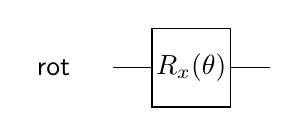
\begin{tikzpicture}[scale=.5] \node[draw=none] at (-3.5, 0) {rot}; \draw (-2,0) -- (-1, 0); \draw (1, 0) -- (2, 0); \draw (-1,-1)--(-1,1)--(1,1)--(1,-1)--cycle; \node[draw=none] at (0, 0) {$R_x(\theta)$}; \end{tikzpicture} } \]


\begin{DoxyParams}[1]{Parameters}
\mbox{\tt in,out}  & {\em multi\+Qubit} & object representing the set of all qubits \\
\hline
\mbox{\tt in}  & {\em rot\+Qubit} & qubit to rotate \\
\hline
\mbox{\tt in}  & {\em angle} & angle by which to rotate in radians \\
\hline
\end{DoxyParams}

\begin{DoxyExceptions}{Exceptions}
{\em exit\+With\+Error} & if {\ttfamily rot\+Qubit} is outside \mbox{[}0, {\ttfamily multi\+Qubit.\+num\+Qubits}). \\
\hline
\end{DoxyExceptions}


Definition at line 441 of file Qu\+E\+S\+T.\+c.


\begin{DoxyCode}
441                                                                    \{
442 
443     \mbox{\hyperlink{structVector}{Vector}} unitAxis = \{1, 0, 0\};
444     \mbox{\hyperlink{QuEST_8c_a8810423457803005fecd415f4299f40d}{rotateAroundAxis}}(multiQubit, rotQubit, angle, unitAxis);
445 \}
\end{DoxyCode}
\mbox{\Hypertarget{QuEST_8c_ace0d3592d38a990e81a434c4e9681500}\label{QuEST_8c_ace0d3592d38a990e81a434c4e9681500}} 
\index{Qu\+E\+S\+T.\+c@{Qu\+E\+S\+T.\+c}!rotateY@{rotateY}}
\index{rotateY@{rotateY}!Qu\+E\+S\+T.\+c@{Qu\+E\+S\+T.\+c}}
\paragraph{\texorpdfstring{rotate\+Y()}{rotateY()}}
{\footnotesize\ttfamily void rotateY (\begin{DoxyParamCaption}\item[{\mbox{\hyperlink{structMultiQubit}{Multi\+Qubit}}}]{multi\+Qubit,  }\item[{const int}]{rot\+Qubit,  }\item[{\mbox{\hyperlink{QuEST__precision_8h_a4b654506f18b8bfd61ad2a29a7e38c25}{R\+E\+AL}}}]{angle }\end{DoxyParamCaption})}



Rotate a single qubit by a given angle around the Y-\/axis of the Bloch-\/sphere. 

For angle $\theta$, applies \[ \begin{pmatrix} \cos\theta/2 & - \sin \theta/2\\ \sin \theta/2 & \cos \theta/2 \end{pmatrix} \] ~\newline
 \[ \setlength{\fboxrule}{0.01pt} \fbox{ 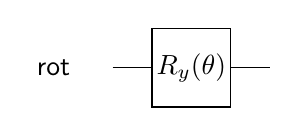
\begin{tikzpicture}[scale=.5] \node[draw=none] at (-3.5, 0) {rot}; \draw (-2,0) -- (-1, 0); \draw (1, 0) -- (2, 0); \draw (-1,-1)--(-1,1)--(1,1)--(1,-1)--cycle; \node[draw=none] at (0, 0) {$R_y(\theta)$}; \end{tikzpicture} } \]


\begin{DoxyParams}[1]{Parameters}
\mbox{\tt in,out}  & {\em multi\+Qubit} & object representing the set of all qubits \\
\hline
\mbox{\tt in}  & {\em rot\+Qubit} & qubit to rotate \\
\hline
\mbox{\tt in}  & {\em angle} & angle by which to rotate in radians \\
\hline
\end{DoxyParams}

\begin{DoxyExceptions}{Exceptions}
{\em exit\+With\+Error} & if {\ttfamily rot\+Qubit} is outside \mbox{[}0, {\ttfamily multi\+Qubit.\+num\+Qubits}). \\
\hline
\end{DoxyExceptions}


Definition at line 447 of file Qu\+E\+S\+T.\+c.



Referenced by main().


\begin{DoxyCode}
447                                                                    \{
448 
449     \mbox{\hyperlink{structVector}{Vector}} unitAxis = \{0, 1, 0\};
450     \mbox{\hyperlink{QuEST_8c_a8810423457803005fecd415f4299f40d}{rotateAroundAxis}}(multiQubit, rotQubit, angle, unitAxis);
451 \}
\end{DoxyCode}
\mbox{\Hypertarget{QuEST_8c_abd621412ad30c1b034f4ce153c4afe10}\label{QuEST_8c_abd621412ad30c1b034f4ce153c4afe10}} 
\index{Qu\+E\+S\+T.\+c@{Qu\+E\+S\+T.\+c}!rotateZ@{rotateZ}}
\index{rotateZ@{rotateZ}!Qu\+E\+S\+T.\+c@{Qu\+E\+S\+T.\+c}}
\paragraph{\texorpdfstring{rotate\+Z()}{rotateZ()}}
{\footnotesize\ttfamily void rotateZ (\begin{DoxyParamCaption}\item[{\mbox{\hyperlink{structMultiQubit}{Multi\+Qubit}}}]{multi\+Qubit,  }\item[{const int}]{rot\+Qubit,  }\item[{\mbox{\hyperlink{QuEST__precision_8h_a4b654506f18b8bfd61ad2a29a7e38c25}{R\+E\+AL}}}]{angle }\end{DoxyParamCaption})}



Rotate a single qubit by a given angle around the Z-\/axis of the Bloch-\/sphere (also known as a phase shift gate). 

For angle $\theta$, applies \[ \begin{pmatrix} \exp(-i \theta/2) & 0 \\ 0 & \exp(i \theta/2) \end{pmatrix} \]

\[ \setlength{\fboxrule}{0.01pt} \fbox{ 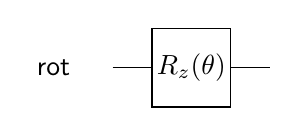
\begin{tikzpicture}[scale=.5] \node[draw=none] at (-3.5, 0) {rot}; \draw (-2,0) -- (-1, 0); \draw (1, 0) -- (2, 0); \draw (-1,-1)--(-1,1)--(1,1)--(1,-1)--cycle; \node[draw=none] at (0, 0) {$R_z(\theta)$}; \end{tikzpicture} } \]


\begin{DoxyParams}[1]{Parameters}
\mbox{\tt in,out}  & {\em multi\+Qubit} & object representing the set of all qubits \\
\hline
\mbox{\tt in}  & {\em rot\+Qubit} & qubit to rotate \\
\hline
\mbox{\tt in}  & {\em angle} & angle by which to rotate in radians \\
\hline
\end{DoxyParams}

\begin{DoxyExceptions}{Exceptions}
{\em exit\+With\+Error} & if {\ttfamily rot\+Qubit} is outside \mbox{[}0, {\ttfamily multi\+Qubit.\+num\+Qubits}). \\
\hline
\end{DoxyExceptions}


Definition at line 453 of file Qu\+E\+S\+T.\+c.


\begin{DoxyCode}
453                                                                    \{
454 
455     \mbox{\hyperlink{structVector}{Vector}} unitAxis = \{0, 0, 1\};
456     \mbox{\hyperlink{QuEST_8c_a8810423457803005fecd415f4299f40d}{rotateAroundAxis}}(multiQubit, rotQubit, angle, unitAxis);
457 \}
\end{DoxyCode}
\mbox{\Hypertarget{QuEST_8c_a95012dad46509b4b461974c34cfd7b3d}\label{QuEST_8c_a95012dad46509b4b461974c34cfd7b3d}} 
\index{Qu\+E\+S\+T.\+c@{Qu\+E\+S\+T.\+c}!seed\+Qu\+E\+ST@{seed\+Qu\+E\+ST}}
\index{seed\+Qu\+E\+ST@{seed\+Qu\+E\+ST}!Qu\+E\+S\+T.\+c@{Qu\+E\+S\+T.\+c}}
\paragraph{\texorpdfstring{seed\+Qu\+E\+S\+T()}{seedQuEST()}}
{\footnotesize\ttfamily void seed\+Qu\+E\+ST (\begin{DoxyParamCaption}\item[{unsigned long int $\ast$}]{seed\+Array,  }\item[{int}]{num\+Seeds }\end{DoxyParamCaption})}



num\+Seeds $<$= 64 

Seed the Mersenne Twister used for random number generation in the Qu\+E\+ST environment with a user defined seed. 

Definition at line 2019 of file Qu\+E\+S\+T.\+c.



Referenced by test\+\_\+measure().


\begin{DoxyCode}
2019                                                           \{
2020     \textcolor{comment}{// init MT random number generator with user defined list of seeds}
2021     \textcolor{comment}{// for the MPI version, it is ok that all procs will get the same seed as random numbers will only be }
2022     \textcolor{comment}{// used by the master process}
2023     \mbox{\hyperlink{mt19937ar_8c_ac1283f9b1ed571332f5ffe53545ffc16}{init\_by\_array}}(seedArray, numSeeds); 
2024 \}
\end{DoxyCode}
\mbox{\Hypertarget{QuEST_8c_ab0ab3ec70938712c26988a6aa51263a0}\label{QuEST_8c_ab0ab3ec70938712c26988a6aa51263a0}} 
\index{Qu\+E\+S\+T.\+c@{Qu\+E\+S\+T.\+c}!seed\+Qu\+E\+S\+T\+Default@{seed\+Qu\+E\+S\+T\+Default}}
\index{seed\+Qu\+E\+S\+T\+Default@{seed\+Qu\+E\+S\+T\+Default}!Qu\+E\+S\+T.\+c@{Qu\+E\+S\+T.\+c}}
\paragraph{\texorpdfstring{seed\+Qu\+E\+S\+T\+Default()}{seedQuESTDefault()}}
{\footnotesize\ttfamily void seed\+Qu\+E\+S\+T\+Default (\begin{DoxyParamCaption}\item[{void}]{ }\end{DoxyParamCaption})}



Seed the Mersenne Twister used for random number generation in the Qu\+E\+ST environment with an example defualt seed. 

This default seeding function uses the mt19937 init\+\_\+by\+\_\+array function with three keys -- time, pid and hostname. Subsequent calls to mt19937 genrand functions will use this seeding. For a multi process code, the same seed is given to all process, therefore this seeding is only appropriate to use for functions such as measure where all processes require the same random value.

For more information about the MT, see \href{http://www.math.sci.hiroshima-u.ac.jp/~m-mat/MT/MT2002/emt19937ar.html}{\tt http\+://www.\+math.\+sci.\+hiroshima-\/u.\+ac.\+jp/$\sim$m-\/mat/\+M\+T/\+M\+T2002/emt19937ar.\+html} 

Definition at line 1994 of file Qu\+E\+S\+T.\+c.



Referenced by init\+Qu\+E\+S\+T\+Env().


\begin{DoxyCode}
1994                        \{
1995     \textcolor{comment}{// init MT random number generator with three keys -- time, pid and a hash of hostname }
1996     \textcolor{comment}{// for the MPI version, it is ok that all procs will get the same seed as random numbers will only be }
1997     \textcolor{comment}{// used by the master process}
1998 
1999     \textcolor{keyword}{struct }timeval  tv;
2000     gettimeofday(&tv, NULL);
2001 
2002     \textcolor{keywordtype}{double} time\_in\_mill = 
2003         (tv.tv\_sec) * 1000 + (tv.tv\_usec) / 1000 ; \textcolor{comment}{// convert tv\_sec & tv\_usec to millisecond}
2004 
2005     \textcolor{keywordtype}{unsigned} \textcolor{keywordtype}{long} \textcolor{keywordtype}{int} pid = getpid();
2006     \textcolor{keywordtype}{unsigned} \textcolor{keywordtype}{long} \textcolor{keywordtype}{int} msecs = (\textcolor{keywordtype}{unsigned} \textcolor{keywordtype}{long} int) time\_in\_mill;
2007     \textcolor{keywordtype}{char} hostName[MAXHOSTNAMELEN+1];
2008     gethostname(hostName, \textcolor{keyword}{sizeof}(hostName));
2009     \textcolor{keywordtype}{unsigned} \textcolor{keywordtype}{long} \textcolor{keywordtype}{int} hostNameInt = \mbox{\hyperlink{QuEST_8c_ab76254cfde16f0808476649507a1a2fc}{hashString}}(hostName);
2010 
2011     \textcolor{keywordtype}{unsigned} \textcolor{keywordtype}{long} \textcolor{keywordtype}{int} key[3];
2012     key[0] = msecs; key[1] = pid; key[2] = hostNameInt;
2013     \mbox{\hyperlink{mt19937ar_8c_ac1283f9b1ed571332f5ffe53545ffc16}{init\_by\_array}}(key, 3); 
2014 \}
\end{DoxyCode}
\mbox{\Hypertarget{QuEST_8c_adda6c47876a7676488ed0565a19eaa65}\label{QuEST_8c_adda6c47876a7676488ed0565a19eaa65}} 
\index{Qu\+E\+S\+T.\+c@{Qu\+E\+S\+T.\+c}!s\+Gate@{s\+Gate}}
\index{s\+Gate@{s\+Gate}!Qu\+E\+S\+T.\+c@{Qu\+E\+S\+T.\+c}}
\paragraph{\texorpdfstring{s\+Gate()}{sGate()}}
{\footnotesize\ttfamily void s\+Gate (\begin{DoxyParamCaption}\item[{\mbox{\hyperlink{structMultiQubit}{Multi\+Qubit}}}]{multi\+Qubit,  }\item[{const int}]{target\+Qubit }\end{DoxyParamCaption})}



Apply the single-\/qubit S gate. 

This is a rotation of $\pi/2$ around the Z-\/axis on the Bloch sphere, or the unitary\+: \[ \begin{pmatrix} 1 & 0 \\ 0 & i \end{pmatrix} \]

\[ \setlength{\fboxrule}{0.01pt} \fbox{ 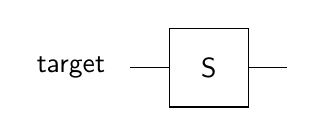
\begin{tikzpicture}[scale=.5] \node[draw=none] at (-3.5, 0) {target}; \draw (-2,0) -- (-1, 0); \draw (1, 0) -- (2, 0); \draw (-1,-1)--(-1,1)--(1,1)--(1,-1)--cycle; \node[draw=none] at (0, 0) {S}; \end{tikzpicture} } \]


\begin{DoxyParams}[1]{Parameters}
\mbox{\tt in,out}  & {\em multi\+Qubit} & object representing the set of all qubits \\
\hline
\mbox{\tt in}  & {\em target\+Qubit} & qubit to operate upon \\
\hline
\end{DoxyParams}

\begin{DoxyExceptions}{Exceptions}
{\em exit\+With\+Error} & if {\ttfamily target\+Qubit} is outside \mbox{[}0, {\ttfamily multi\+Qubit.\+num\+Qubits}) \\
\hline
\end{DoxyExceptions}


Definition at line 1626 of file Qu\+E\+S\+T.\+c.



Referenced by test\+\_\+s\+Gate().


\begin{DoxyCode}
1627 \{
1628     \mbox{\hyperlink{QuEST__env__local_8c_aae7a8a7f1ccbddb7f76b6c52b746bb43}{phaseGate}}(multiQubit, targetQubit, \mbox{\hyperlink{QuEST_8h_a5739021c733cecc49647956b2f7338eaa06e60f80fa80cce271793d6d31bcc21f}{S\_GATE}});
1629 \} 
\end{DoxyCode}
\mbox{\Hypertarget{QuEST_8c_a2275fff50824fe47485890ff5a857785}\label{QuEST_8c_a2275fff50824fe47485890ff5a857785}} 
\index{Qu\+E\+S\+T.\+c@{Qu\+E\+S\+T.\+c}!sigma\+X\+Distributed@{sigma\+X\+Distributed}}
\index{sigma\+X\+Distributed@{sigma\+X\+Distributed}!Qu\+E\+S\+T.\+c@{Qu\+E\+S\+T.\+c}}
\paragraph{\texorpdfstring{sigma\+X\+Distributed()}{sigmaXDistributed()}}
{\footnotesize\ttfamily void sigma\+X\+Distributed (\begin{DoxyParamCaption}\item[{\mbox{\hyperlink{structMultiQubit}{Multi\+Qubit}}}]{multi\+Qubit,  }\item[{const int}]{target\+Qubit,  }\item[{\mbox{\hyperlink{structComplexArray}{Complex\+Array}}}]{state\+Vec\+In,  }\item[{\mbox{\hyperlink{structComplexArray}{Complex\+Array}}}]{state\+Vec\+Out }\end{DoxyParamCaption})}



Rotate a single qubit by \{\{0,1\},\{1,0\}. 

Operate on a subset of the state vector with upper and lower block values stored seperately. This rotation is just swapping upper and lower values, and state\+Vec\+In must already be the correct section for this chunk

\begin{DoxyRemark}{Remarks}
Qubits are zero-\/based and the ~\newline
the first qubit is the rightmost ~\newline
 
\end{DoxyRemark}

\begin{DoxyParams}[1]{Parameters}
\mbox{\tt in,out}  & {\em multi\+Qubit} & object representing the set of qubits \\
\hline
\mbox{\tt in}  & {\em target\+Qubit} & qubit to rotate \\
\hline
\mbox{\tt in}  & {\em state\+Vec\+In} & probability amplitudes in lower or upper half of a block depending on chunk\+Id \\
\hline
\mbox{\tt out}  & {\em state\+Vec\+Out} & array section to update (will correspond to either the lower or upper half of a block) \\
\hline
\end{DoxyParams}


Definition at line 1165 of file Qu\+E\+S\+T.\+c.



References Complex\+Array\+::imag, Multi\+Qubit\+::num\+Amps\+Per\+Chunk, Complex\+Array\+::real, and R\+E\+AL.



Referenced by sigma\+X().


\begin{DoxyCode}
1168 \{
1169 
1170     \textcolor{keywordtype}{long} \textcolor{keywordtype}{long} \textcolor{keywordtype}{int} thisTask;  
1171     \textcolor{keyword}{const} \textcolor{keywordtype}{long} \textcolor{keywordtype}{long} \textcolor{keywordtype}{int} numTasks=multiQubit.\mbox{\hyperlink{structMultiQubit_a1cad83601a78635dd278259c7ed54f18}{numAmpsPerChunk}};
1172 
1173     \mbox{\hyperlink{QuEST__precision_8h_a4b654506f18b8bfd61ad2a29a7e38c25}{REAL}} *stateVecRealIn=stateVecIn.\mbox{\hyperlink{structComplexArray_a4195cac6c784ea1b6271f1c7dba1548a}{real}}, *stateVecImagIn=stateVecIn.
      \mbox{\hyperlink{structComplexArray_a79dde47c7ae530c79cebfdf57b225968}{imag}};
1174     \mbox{\hyperlink{QuEST__precision_8h_a4b654506f18b8bfd61ad2a29a7e38c25}{REAL}} *stateVecRealOut=stateVecOut.\mbox{\hyperlink{structComplexArray_a4195cac6c784ea1b6271f1c7dba1548a}{real}}, *stateVecImagOut=stateVecOut.
      \mbox{\hyperlink{structComplexArray_a79dde47c7ae530c79cebfdf57b225968}{imag}};
1175 
1176 \textcolor{preprocessor}{# ifdef \_OPENMP}
1177 \textcolor{preprocessor}{# pragma omp parallel \(\backslash\)}
1178 \textcolor{preprocessor}{    default  (none) \(\backslash\)}
1179 \textcolor{preprocessor}{    shared   (stateVecRealIn,stateVecImagIn,stateVecRealOut,stateVecImagOut) \(\backslash\)}
1180 \textcolor{preprocessor}{    private  (thisTask)}
1181 \textcolor{preprocessor}{# endif}
1182     \{
1183 \textcolor{preprocessor}{# ifdef \_OPENMP}
1184 \textcolor{preprocessor}{# pragma omp for schedule (static)}
1185 \textcolor{preprocessor}{# endif}
1186         \textcolor{keywordflow}{for} (thisTask=0; thisTask<numTasks; thisTask++) \{
1187             stateVecRealOut[thisTask] = stateVecRealIn[thisTask];
1188             stateVecImagOut[thisTask] = stateVecImagIn[thisTask];
1189         \}
1190     \}
1191 \} 
\end{DoxyCode}
\mbox{\Hypertarget{QuEST_8c_a74822fd86bb5d81766e6e8dbdcd62df1}\label{QuEST_8c_a74822fd86bb5d81766e6e8dbdcd62df1}} 
\index{Qu\+E\+S\+T.\+c@{Qu\+E\+S\+T.\+c}!sigma\+X\+Local@{sigma\+X\+Local}}
\index{sigma\+X\+Local@{sigma\+X\+Local}!Qu\+E\+S\+T.\+c@{Qu\+E\+S\+T.\+c}}
\paragraph{\texorpdfstring{sigma\+X\+Local()}{sigmaXLocal()}}
{\footnotesize\ttfamily void sigma\+X\+Local (\begin{DoxyParamCaption}\item[{\mbox{\hyperlink{structMultiQubit}{Multi\+Qubit}}}]{multi\+Qubit,  }\item[{const int}]{target\+Qubit }\end{DoxyParamCaption})}



Definition at line 1106 of file Qu\+E\+S\+T.\+c.



References Complex\+Array\+::imag, Multi\+Qubit\+::num\+Amps\+Per\+Chunk, Complex\+Array\+::real, R\+E\+AL, and Multi\+Qubit\+::state\+Vec.



Referenced by sigma\+X().


\begin{DoxyCode}
1107 \{
1108     \textcolor{keywordtype}{long} \textcolor{keywordtype}{long} \textcolor{keywordtype}{int} sizeBlock, sizeHalfBlock;
1109     \textcolor{keywordtype}{long} \textcolor{keywordtype}{long} \textcolor{keywordtype}{int} thisBlock, \textcolor{comment}{// current block}
1110          indexUp,indexLo;    \textcolor{comment}{// current index and corresponding index in lower half block}
1111 
1112     \mbox{\hyperlink{QuEST__precision_8h_a4b654506f18b8bfd61ad2a29a7e38c25}{REAL}} stateRealUp,stateImagUp;
1113     \textcolor{keywordtype}{long} \textcolor{keywordtype}{long} \textcolor{keywordtype}{int} thisTask;         
1114     \textcolor{keyword}{const} \textcolor{keywordtype}{long} \textcolor{keywordtype}{long} \textcolor{keywordtype}{int} numTasks=multiQubit.\mbox{\hyperlink{structMultiQubit_a1cad83601a78635dd278259c7ed54f18}{numAmpsPerChunk}}>>1;
1115 
1116     \textcolor{comment}{// set dimensions}
1117     sizeHalfBlock = 1LL << targetQubit;  
1118     sizeBlock     = 2LL * sizeHalfBlock; 
1119 
1120     \textcolor{comment}{// Can't use multiQubit.stateVec as a private OMP var}
1121     \mbox{\hyperlink{QuEST__precision_8h_a4b654506f18b8bfd61ad2a29a7e38c25}{REAL}} *stateVecReal = multiQubit.\mbox{\hyperlink{structMultiQubit_a45483190d6b01ef6b2f98f2bec9ab94f}{stateVec}}.\mbox{\hyperlink{structComplexArray_a4195cac6c784ea1b6271f1c7dba1548a}{real}};
1122     \mbox{\hyperlink{QuEST__precision_8h_a4b654506f18b8bfd61ad2a29a7e38c25}{REAL}} *stateVecImag = multiQubit.\mbox{\hyperlink{structMultiQubit_a45483190d6b01ef6b2f98f2bec9ab94f}{stateVec}}.\mbox{\hyperlink{structComplexArray_a79dde47c7ae530c79cebfdf57b225968}{imag}};
1123 
1124 \textcolor{preprocessor}{# ifdef \_OPENMP}
1125 \textcolor{preprocessor}{# pragma omp parallel \(\backslash\)}
1126 \textcolor{preprocessor}{    default  (none) \(\backslash\)}
1127 \textcolor{preprocessor}{    shared   (sizeBlock,sizeHalfBlock, stateVecReal,stateVecImag) \(\backslash\)}
1128 \textcolor{preprocessor}{    private  (thisTask,thisBlock ,indexUp,indexLo, stateRealUp,stateImagUp) }
1129 \textcolor{preprocessor}{# endif}
1130     \{
1131 \textcolor{preprocessor}{# ifdef \_OPENMP}
1132 \textcolor{preprocessor}{# pragma omp for schedule (static)}
1133 \textcolor{preprocessor}{# endif}
1134         \textcolor{keywordflow}{for} (thisTask=0; thisTask<numTasks; thisTask++) \{
1135             thisBlock   = thisTask / sizeHalfBlock;
1136             indexUp     = thisBlock*sizeBlock + thisTask%sizeHalfBlock;
1137             indexLo     = indexUp + sizeHalfBlock;
1138 
1139             stateRealUp = stateVecReal[indexUp];
1140             stateImagUp = stateVecImag[indexUp];
1141 
1142             stateVecReal[indexUp] = stateVecReal[indexLo];
1143             stateVecImag[indexUp] = stateVecImag[indexLo];
1144 
1145             stateVecReal[indexLo] = stateRealUp;
1146             stateVecImag[indexLo] = stateImagUp;
1147         \} 
1148     \}
1149 
1150 \}
\end{DoxyCode}
\mbox{\Hypertarget{QuEST_8c_af5ef5166f00c0572354b4ac53dcf40cf}\label{QuEST_8c_af5ef5166f00c0572354b4ac53dcf40cf}} 
\index{Qu\+E\+S\+T.\+c@{Qu\+E\+S\+T.\+c}!sigma\+Y\+Distributed@{sigma\+Y\+Distributed}}
\index{sigma\+Y\+Distributed@{sigma\+Y\+Distributed}!Qu\+E\+S\+T.\+c@{Qu\+E\+S\+T.\+c}}
\paragraph{\texorpdfstring{sigma\+Y\+Distributed()}{sigmaYDistributed()}}
{\footnotesize\ttfamily void sigma\+Y\+Distributed (\begin{DoxyParamCaption}\item[{\mbox{\hyperlink{structMultiQubit}{Multi\+Qubit}}}]{multi\+Qubit,  }\item[{const int}]{target\+Qubit,  }\item[{\mbox{\hyperlink{structComplexArray}{Complex\+Array}}}]{state\+Vec\+In,  }\item[{\mbox{\hyperlink{structComplexArray}{Complex\+Array}}}]{state\+Vec\+Out,  }\item[{int}]{update\+Upper }\end{DoxyParamCaption})}



Rotate a single qubit by \{\{0,-\/i\},\{i,0\}. 

Operate on a subset of the state vector with upper and lower block values stored seperately. This rotation is just swapping upper and lower values, and state\+Vec\+In must already be the correct section for this chunk

\begin{DoxyRemark}{Remarks}
Qubits are zero-\/based and the ~\newline
the first qubit is the rightmost ~\newline
 
\end{DoxyRemark}

\begin{DoxyParams}[1]{Parameters}
\mbox{\tt in,out}  & {\em multi\+Qubit} & object representing the set of qubits \\
\hline
\mbox{\tt in}  & {\em target\+Qubit} & qubit to rotate \\
\hline
\mbox{\tt in}  & {\em state\+Vec\+In} & probability amplitudes in lower or upper half of a block depending on chunk\+Id \\
\hline
\mbox{\tt in}  & {\em update\+Upper} & flag, 1\+: updating upper values, 0\+: updating lower values in block \\
\hline
\mbox{\tt out}  & {\em state\+Vec\+Out} & array section to update (will correspond to either the lower or upper half of a block) \\
\hline
\end{DoxyParams}


Definition at line 1352 of file Qu\+E\+S\+T.\+c.



References Complex\+Array\+::imag, Multi\+Qubit\+::num\+Amps\+Per\+Chunk, Complex\+Array\+::real, and R\+E\+AL.



Referenced by sigma\+Y().


\begin{DoxyCode}
1356 \{
1357 
1358     \textcolor{keywordtype}{long} \textcolor{keywordtype}{long} \textcolor{keywordtype}{int} thisTask;  
1359     \textcolor{keyword}{const} \textcolor{keywordtype}{long} \textcolor{keywordtype}{long} \textcolor{keywordtype}{int} numTasks=multiQubit.\mbox{\hyperlink{structMultiQubit_a1cad83601a78635dd278259c7ed54f18}{numAmpsPerChunk}};
1360 
1361     \mbox{\hyperlink{QuEST__precision_8h_a4b654506f18b8bfd61ad2a29a7e38c25}{REAL}} *stateVecRealIn=stateVecIn.\mbox{\hyperlink{structComplexArray_a4195cac6c784ea1b6271f1c7dba1548a}{real}}, *stateVecImagIn=stateVecIn.
      \mbox{\hyperlink{structComplexArray_a79dde47c7ae530c79cebfdf57b225968}{imag}};
1362     \mbox{\hyperlink{QuEST__precision_8h_a4b654506f18b8bfd61ad2a29a7e38c25}{REAL}} *stateVecRealOut=stateVecOut.\mbox{\hyperlink{structComplexArray_a4195cac6c784ea1b6271f1c7dba1548a}{real}}, *stateVecImagOut=stateVecOut.
      \mbox{\hyperlink{structComplexArray_a79dde47c7ae530c79cebfdf57b225968}{imag}};
1363 
1364     \textcolor{keywordtype}{int} realSign=1, imagSign=1;
1365     \textcolor{keywordflow}{if} (updateUpper) imagSign=-1;
1366     \textcolor{keywordflow}{else} realSign = -1;
1367 
1368 \textcolor{preprocessor}{# ifdef \_OPENMP}
1369 \textcolor{preprocessor}{# pragma omp parallel \(\backslash\)}
1370 \textcolor{preprocessor}{    default  (none) \(\backslash\)}
1371 \textcolor{preprocessor}{    shared   (stateVecRealIn,stateVecImagIn,stateVecRealOut,stateVecImagOut,realSign,imagSign) \(\backslash\)}
1372 \textcolor{preprocessor}{    private  (thisTask)}
1373 \textcolor{preprocessor}{# endif}
1374     \{
1375 \textcolor{preprocessor}{# ifdef \_OPENMP}
1376 \textcolor{preprocessor}{# pragma omp for schedule (static)}
1377 \textcolor{preprocessor}{# endif}
1378         \textcolor{keywordflow}{for} (thisTask=0; thisTask<numTasks; thisTask++) \{
1379             stateVecRealOut[thisTask] = realSign*stateVecImagIn[thisTask];
1380             stateVecImagOut[thisTask] = imagSign*stateVecRealIn[thisTask];
1381         \}
1382     \}
1383 \} 
\end{DoxyCode}
\mbox{\Hypertarget{QuEST_8c_a81fbfaed65a742a7dfd622e17652245e}\label{QuEST_8c_a81fbfaed65a742a7dfd622e17652245e}} 
\index{Qu\+E\+S\+T.\+c@{Qu\+E\+S\+T.\+c}!sigma\+Y\+Local@{sigma\+Y\+Local}}
\index{sigma\+Y\+Local@{sigma\+Y\+Local}!Qu\+E\+S\+T.\+c@{Qu\+E\+S\+T.\+c}}
\paragraph{\texorpdfstring{sigma\+Y\+Local()}{sigmaYLocal()}}
{\footnotesize\ttfamily void sigma\+Y\+Local (\begin{DoxyParamCaption}\item[{\mbox{\hyperlink{structMultiQubit}{Multi\+Qubit}}}]{multi\+Qubit,  }\item[{const int}]{target\+Qubit }\end{DoxyParamCaption})}



Definition at line 1293 of file Qu\+E\+S\+T.\+c.



References Complex\+Array\+::imag, Multi\+Qubit\+::num\+Amps\+Per\+Chunk, Complex\+Array\+::real, R\+E\+AL, and Multi\+Qubit\+::state\+Vec.



Referenced by sigma\+Y().


\begin{DoxyCode}
1294 \{
1295     \textcolor{keywordtype}{long} \textcolor{keywordtype}{long} \textcolor{keywordtype}{int} sizeBlock, sizeHalfBlock;
1296     \textcolor{keywordtype}{long} \textcolor{keywordtype}{long} \textcolor{keywordtype}{int} thisBlock, \textcolor{comment}{// current block}
1297          indexUp,indexLo;    \textcolor{comment}{// current index and corresponding index in lower half block}
1298 
1299     \mbox{\hyperlink{QuEST__precision_8h_a4b654506f18b8bfd61ad2a29a7e38c25}{REAL}} stateRealUp,stateImagUp;
1300     \textcolor{keywordtype}{long} \textcolor{keywordtype}{long} \textcolor{keywordtype}{int} thisTask;         
1301     \textcolor{keyword}{const} \textcolor{keywordtype}{long} \textcolor{keywordtype}{long} \textcolor{keywordtype}{int} numTasks=multiQubit.\mbox{\hyperlink{structMultiQubit_a1cad83601a78635dd278259c7ed54f18}{numAmpsPerChunk}}>>1;
1302 
1303     \textcolor{comment}{// set dimensions}
1304     sizeHalfBlock = 1LL << targetQubit;  
1305     sizeBlock     = 2LL * sizeHalfBlock; 
1306 
1307     \textcolor{comment}{// Can't use multiQubit.stateVec as a private OMP var}
1308     \mbox{\hyperlink{QuEST__precision_8h_a4b654506f18b8bfd61ad2a29a7e38c25}{REAL}} *stateVecReal = multiQubit.\mbox{\hyperlink{structMultiQubit_a45483190d6b01ef6b2f98f2bec9ab94f}{stateVec}}.\mbox{\hyperlink{structComplexArray_a4195cac6c784ea1b6271f1c7dba1548a}{real}};
1309     \mbox{\hyperlink{QuEST__precision_8h_a4b654506f18b8bfd61ad2a29a7e38c25}{REAL}} *stateVecImag = multiQubit.\mbox{\hyperlink{structMultiQubit_a45483190d6b01ef6b2f98f2bec9ab94f}{stateVec}}.\mbox{\hyperlink{structComplexArray_a79dde47c7ae530c79cebfdf57b225968}{imag}};
1310 
1311 \textcolor{preprocessor}{# ifdef \_OPENMP}
1312 \textcolor{preprocessor}{# pragma omp parallel \(\backslash\)}
1313 \textcolor{preprocessor}{    default  (none) \(\backslash\)}
1314 \textcolor{preprocessor}{    shared   (sizeBlock,sizeHalfBlock, stateVecReal,stateVecImag) \(\backslash\)}
1315 \textcolor{preprocessor}{    private  (thisTask,thisBlock ,indexUp,indexLo, stateRealUp,stateImagUp) }
1316 \textcolor{preprocessor}{# endif}
1317     \{
1318 \textcolor{preprocessor}{# ifdef \_OPENMP}
1319 \textcolor{preprocessor}{# pragma omp for schedule (static)}
1320 \textcolor{preprocessor}{# endif}
1321         \textcolor{keywordflow}{for} (thisTask=0; thisTask<numTasks; thisTask++) \{
1322             thisBlock   = thisTask / sizeHalfBlock;
1323             indexUp     = thisBlock*sizeBlock + thisTask%sizeHalfBlock;
1324             indexLo     = indexUp + sizeHalfBlock;
1325 
1326             stateRealUp = stateVecReal[indexUp];
1327             stateImagUp = stateVecImag[indexUp];
1328 
1329             stateVecReal[indexUp] = stateVecImag[indexLo];
1330             stateVecImag[indexUp] = -stateVecReal[indexLo];
1331 
1332             stateVecReal[indexLo] = -stateImagUp;
1333             stateVecImag[indexLo] = stateRealUp;
1334         \} 
1335     \}
1336 \}
\end{DoxyCode}
\mbox{\Hypertarget{QuEST_8c_aebaab86326779de55d335cfea3efde8f}\label{QuEST_8c_aebaab86326779de55d335cfea3efde8f}} 
\index{Qu\+E\+S\+T.\+c@{Qu\+E\+S\+T.\+c}!sigmaZ@{sigmaZ}}
\index{sigmaZ@{sigmaZ}!Qu\+E\+S\+T.\+c@{Qu\+E\+S\+T.\+c}}
\paragraph{\texorpdfstring{sigma\+Z()}{sigmaZ()}}
{\footnotesize\ttfamily void sigmaZ (\begin{DoxyParamCaption}\item[{\mbox{\hyperlink{structMultiQubit}{Multi\+Qubit}}}]{multi\+Qubit,  }\item[{const int}]{target\+Qubit }\end{DoxyParamCaption})}



Apply the single-\/qubit sigma-\/Z (also known as the Z, Pauli-\/Z or phase-\/flip) gate. 

This is a rotation of $\pi$ around the Z-\/axis (a phase shift) on the Bloch sphere. I.\+e. \[ \begin{pmatrix} 1 & 0 \\ 0 & -1 \end{pmatrix} \] ~\newline
 \[ \setlength{\fboxrule}{0.01pt} \fbox{ 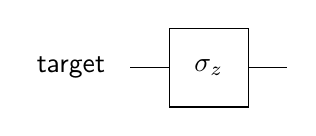
\begin{tikzpicture}[scale=.5] \node[draw=none] at (-3.5, 0) {target}; \draw (-2,0) -- (-1, 0); \draw (1, 0) -- (2, 0); \draw (-1,-1)--(-1,1)--(1,1)--(1,-1)--cycle; \node[draw=none] at (0, 0) {$\sigma_z$}; \end{tikzpicture} } \] ~\newline
 
\begin{DoxyParams}[1]{Parameters}
\mbox{\tt in,out}  & {\em multi\+Qubit} & object representing the set of all qubits \\
\hline
\mbox{\tt in}  & {\em target\+Qubit} & qubit to operate on \\
\hline
\end{DoxyParams}

\begin{DoxyExceptions}{Exceptions}
{\em exit\+With\+Error} & if {\ttfamily target\+Qubit} is outside \mbox{[}0, {\ttfamily multi\+Qubit.\+num\+Qubits}). \\
\hline
\end{DoxyExceptions}


Definition at line 1621 of file Qu\+E\+S\+T.\+c.



Referenced by test\+\_\+sigma\+Z().


\begin{DoxyCode}
1622 \{
1623     \mbox{\hyperlink{QuEST__env__local_8c_aae7a8a7f1ccbddb7f76b6c52b746bb43}{phaseGate}}(multiQubit, targetQubit, \mbox{\hyperlink{QuEST_8h_a5739021c733cecc49647956b2f7338eaa754922d1e1846a1961ff2bf163483dac}{SIGMA\_Z}});
1624 \}
\end{DoxyCode}
\mbox{\Hypertarget{QuEST_8c_af764ea63a2e870098f4e1ce08562942e}\label{QuEST_8c_af764ea63a2e870098f4e1ce08562942e}} 
\index{Qu\+E\+S\+T.\+c@{Qu\+E\+S\+T.\+c}!t\+Gate@{t\+Gate}}
\index{t\+Gate@{t\+Gate}!Qu\+E\+S\+T.\+c@{Qu\+E\+S\+T.\+c}}
\paragraph{\texorpdfstring{t\+Gate()}{tGate()}}
{\footnotesize\ttfamily void t\+Gate (\begin{DoxyParamCaption}\item[{\mbox{\hyperlink{structMultiQubit}{Multi\+Qubit}}}]{multi\+Qubit,  }\item[{const int}]{target\+Qubit }\end{DoxyParamCaption})}



Apply the single-\/qubit T gate. 

This is a rotation of $\pi/4$ around the Z-\/axis on the Bloch sphere, or the unitary\+: \[ \begin{pmatrix} 1 & 0 \\ 0 & \exp\left(i \frac{\pi}{4}\right) \end{pmatrix} \]

\[ \setlength{\fboxrule}{0.01pt} \fbox{ 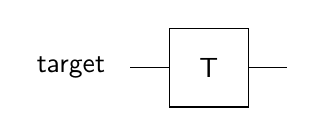
\begin{tikzpicture}[scale=.5] \node[draw=none] at (-3.5, 0) {target}; \draw (-2,0) -- (-1, 0); \draw (1, 0) -- (2, 0); \draw (-1,-1)--(-1,1)--(1,1)--(1,-1)--cycle; \node[draw=none] at (0, 0) {T}; \end{tikzpicture} } \]


\begin{DoxyParams}[1]{Parameters}
\mbox{\tt in,out}  & {\em multi\+Qubit} & object representing the set of all qubits \\
\hline
\mbox{\tt in}  & {\em target\+Qubit} & qubit to operate upon \\
\hline
\end{DoxyParams}

\begin{DoxyExceptions}{Exceptions}
{\em exit\+With\+Error} & if {\ttfamily target\+Qubit} is outside \mbox{[}0, {\ttfamily multi\+Qubit.\+num\+Qubits}) \\
\hline
\end{DoxyExceptions}


Definition at line 1631 of file Qu\+E\+S\+T.\+c.



Referenced by test\+\_\+t\+Gate().


\begin{DoxyCode}
1632 \{
1633     \mbox{\hyperlink{QuEST__env__local_8c_aae7a8a7f1ccbddb7f76b6c52b746bb43}{phaseGate}}(multiQubit, targetQubit, \mbox{\hyperlink{QuEST_8h_a5739021c733cecc49647956b2f7338eaa614d07d597a8e320cc556bc0e652e4ab}{T\_GATE}});
1634 \}
\end{DoxyCode}
\mbox{\Hypertarget{QuEST_8c_a2343b7240118e89aa615e2c9140b770b}\label{QuEST_8c_a2343b7240118e89aa615e2c9140b770b}} 
\index{Qu\+E\+S\+T.\+c@{Qu\+E\+S\+T.\+c}!unitary\+Distributed@{unitary\+Distributed}}
\index{unitary\+Distributed@{unitary\+Distributed}!Qu\+E\+S\+T.\+c@{Qu\+E\+S\+T.\+c}}
\paragraph{\texorpdfstring{unitary\+Distributed()}{unitaryDistributed()}}
{\footnotesize\ttfamily void unitary\+Distributed (\begin{DoxyParamCaption}\item[{\mbox{\hyperlink{structMultiQubit}{Multi\+Qubit}}}]{multi\+Qubit,  }\item[{const int}]{target\+Qubit,  }\item[{\mbox{\hyperlink{structComplex}{Complex}}}]{rot1,  }\item[{\mbox{\hyperlink{structComplex}{Complex}}}]{rot2,  }\item[{\mbox{\hyperlink{structComplexArray}{Complex\+Array}}}]{state\+Vec\+Up,  }\item[{\mbox{\hyperlink{structComplexArray}{Complex\+Array}}}]{state\+Vec\+Lo,  }\item[{\mbox{\hyperlink{structComplexArray}{Complex\+Array}}}]{state\+Vec\+Out }\end{DoxyParamCaption})}



Apply a unitary operation to a single qubit given a subset of the state vector with upper and lower block values stored seperately. 

\begin{DoxyRemark}{Remarks}
Qubits are zero-\/based and the first qubit is the rightmost ~\newline
 
\end{DoxyRemark}

\begin{DoxyParams}[1]{Parameters}
\mbox{\tt in,out}  & {\em multi\+Qubit} & object representing the set of qubits \\
\hline
\mbox{\tt in}  & {\em target\+Qubit} & qubit to rotate \\
\hline
\mbox{\tt in}  & {\em u} & unitary matrix to apply \\
\hline
\mbox{\tt in}  & {\em state\+Vec\+Up} & probability amplitudes in upper half of a block \\
\hline
\mbox{\tt in}  & {\em state\+Vec\+Lo} & probability amplitudes in lower half of a block \\
\hline
\mbox{\tt out}  & {\em state\+Vec\+Out} & array section to update (will correspond to either the lower or upper half of a block) \\
\hline
\end{DoxyParams}


Definition at line 675 of file Qu\+E\+S\+T.\+c.



References Complex\+Array\+::imag, Complex\+::imag, Multi\+Qubit\+::num\+Amps\+Per\+Chunk, Complex\+Array\+::real, R\+E\+AL, and Complex\+::real.



Referenced by unitary().


\begin{DoxyCode}
680 \{
681 
682     \mbox{\hyperlink{QuEST__precision_8h_a4b654506f18b8bfd61ad2a29a7e38c25}{REAL}}   stateRealUp,stateRealLo,stateImagUp,stateImagLo;
683     \textcolor{keywordtype}{long} \textcolor{keywordtype}{long} \textcolor{keywordtype}{int} thisTask;  
684     \textcolor{keyword}{const} \textcolor{keywordtype}{long} \textcolor{keywordtype}{long} \textcolor{keywordtype}{int} numTasks=multiQubit.\mbox{\hyperlink{structMultiQubit_a1cad83601a78635dd278259c7ed54f18}{numAmpsPerChunk}};
685 
686     \mbox{\hyperlink{QuEST__precision_8h_a4b654506f18b8bfd61ad2a29a7e38c25}{REAL}} rot1Real=rot1.\mbox{\hyperlink{structComplex_a479ad939835457595fcca3ca55c06283}{real}}, rot1Imag=rot1.\mbox{\hyperlink{structComplex_a1151948284b21c0052f203f23ab931d9}{imag}};
687     \mbox{\hyperlink{QuEST__precision_8h_a4b654506f18b8bfd61ad2a29a7e38c25}{REAL}} rot2Real=rot2.\mbox{\hyperlink{structComplex_a479ad939835457595fcca3ca55c06283}{real}}, rot2Imag=rot2.\mbox{\hyperlink{structComplex_a1151948284b21c0052f203f23ab931d9}{imag}};
688     \mbox{\hyperlink{QuEST__precision_8h_a4b654506f18b8bfd61ad2a29a7e38c25}{REAL}} *stateVecRealUp=stateVecUp.\mbox{\hyperlink{structComplexArray_a4195cac6c784ea1b6271f1c7dba1548a}{real}}, *stateVecImagUp=stateVecUp.
      \mbox{\hyperlink{structComplexArray_a79dde47c7ae530c79cebfdf57b225968}{imag}};
689     \mbox{\hyperlink{QuEST__precision_8h_a4b654506f18b8bfd61ad2a29a7e38c25}{REAL}} *stateVecRealLo=stateVecLo.\mbox{\hyperlink{structComplexArray_a4195cac6c784ea1b6271f1c7dba1548a}{real}}, *stateVecImagLo=stateVecLo.
      \mbox{\hyperlink{structComplexArray_a79dde47c7ae530c79cebfdf57b225968}{imag}};
690     \mbox{\hyperlink{QuEST__precision_8h_a4b654506f18b8bfd61ad2a29a7e38c25}{REAL}} *stateVecRealOut=stateVecOut.\mbox{\hyperlink{structComplexArray_a4195cac6c784ea1b6271f1c7dba1548a}{real}}, *stateVecImagOut=stateVecOut.
      \mbox{\hyperlink{structComplexArray_a79dde47c7ae530c79cebfdf57b225968}{imag}};
691 
692 
693 \textcolor{preprocessor}{# ifdef \_OPENMP}
694 \textcolor{preprocessor}{# pragma omp parallel \(\backslash\)}
695 \textcolor{preprocessor}{    default  (none) \(\backslash\)}
696 \textcolor{preprocessor}{    shared   (stateVecRealUp,stateVecImagUp,stateVecRealLo,stateVecImagLo,stateVecRealOut,stateVecImagOut, 
      \(\backslash\)}
697 \textcolor{preprocessor}{            rot1Real, rot1Imag, rot2Real, rot2Imag) \(\backslash\)}
698 \textcolor{preprocessor}{    private  (thisTask,stateRealUp,stateImagUp,stateRealLo,stateImagLo)}
699 \textcolor{preprocessor}{# endif}
700     \{
701 \textcolor{preprocessor}{# ifdef \_OPENMP}
702 \textcolor{preprocessor}{# pragma omp for schedule (static)}
703 \textcolor{preprocessor}{# endif}
704         \textcolor{keywordflow}{for} (thisTask=0; thisTask<numTasks; thisTask++) \{
705             \textcolor{comment}{// store current state vector values in temp variables}
706             stateRealUp = stateVecRealUp[thisTask];
707             stateImagUp = stateVecImagUp[thisTask];
708 
709             stateRealLo = stateVecRealLo[thisTask];
710             stateImagLo = stateVecImagLo[thisTask];
711 
712             stateVecRealOut[thisTask] = rot1Real*stateRealUp - rot1Imag*stateImagUp 
713                 + rot2Real*stateRealLo - rot2Imag*stateImagLo;
714             stateVecImagOut[thisTask] = rot1Real*stateImagUp + rot1Imag*stateRealUp 
715                 + rot2Real*stateImagLo + rot2Imag*stateRealLo;
716         \}
717     \}
718 \}
\end{DoxyCode}
\mbox{\Hypertarget{QuEST_8c_ac134fb45b0a7248c5d15e16eb7139a35}\label{QuEST_8c_ac134fb45b0a7248c5d15e16eb7139a35}} 
\index{Qu\+E\+S\+T.\+c@{Qu\+E\+S\+T.\+c}!unitary\+Local@{unitary\+Local}}
\index{unitary\+Local@{unitary\+Local}!Qu\+E\+S\+T.\+c@{Qu\+E\+S\+T.\+c}}
\paragraph{\texorpdfstring{unitary\+Local()}{unitaryLocal()}}
{\footnotesize\ttfamily void unitary\+Local (\begin{DoxyParamCaption}\item[{\mbox{\hyperlink{structMultiQubit}{Multi\+Qubit}}}]{multi\+Qubit,  }\item[{const int}]{target\+Qubit,  }\item[{\mbox{\hyperlink{structComplexMatrix2}{Complex\+Matrix2}}}]{u }\end{DoxyParamCaption})}



Definition at line 549 of file Qu\+E\+S\+T.\+c.



References Complex\+Array\+::imag, Complex\+::imag, Multi\+Qubit\+::num\+Amps\+Per\+Chunk, Complex\+Matrix2\+::r0c0, Complex\+Matrix2\+::r0c1, Complex\+Matrix2\+::r1c0, Complex\+Matrix2\+::r1c1, Complex\+Array\+::real, R\+E\+AL, Complex\+::real, and Multi\+Qubit\+::state\+Vec.



Referenced by unitary().


\begin{DoxyCode}
550 \{
551     \textcolor{keywordtype}{long} \textcolor{keywordtype}{long} \textcolor{keywordtype}{int} sizeBlock, sizeHalfBlock;
552     \textcolor{keywordtype}{long} \textcolor{keywordtype}{long} \textcolor{keywordtype}{int} thisBlock, \textcolor{comment}{// current block}
553          indexUp,indexLo;    \textcolor{comment}{// current index and corresponding index in lower half block}
554 
555     \mbox{\hyperlink{QuEST__precision_8h_a4b654506f18b8bfd61ad2a29a7e38c25}{REAL}} stateRealUp,stateRealLo,stateImagUp,stateImagLo;
556     \textcolor{keywordtype}{long} \textcolor{keywordtype}{long} \textcolor{keywordtype}{int} thisTask;         
557     \textcolor{keyword}{const} \textcolor{keywordtype}{long} \textcolor{keywordtype}{long} \textcolor{keywordtype}{int} numTasks=multiQubit.\mbox{\hyperlink{structMultiQubit_a1cad83601a78635dd278259c7ed54f18}{numAmpsPerChunk}}>>1;
558 
559     \textcolor{comment}{// set dimensions}
560     sizeHalfBlock = 1LL << targetQubit;  
561     sizeBlock     = 2LL * sizeHalfBlock; 
562 
563     \textcolor{comment}{// Can't use multiQubit.stateVec as a private OMP var}
564     \mbox{\hyperlink{QuEST__precision_8h_a4b654506f18b8bfd61ad2a29a7e38c25}{REAL}} *stateVecReal = multiQubit.\mbox{\hyperlink{structMultiQubit_a45483190d6b01ef6b2f98f2bec9ab94f}{stateVec}}.\mbox{\hyperlink{structComplexArray_a4195cac6c784ea1b6271f1c7dba1548a}{real}};
565     \mbox{\hyperlink{QuEST__precision_8h_a4b654506f18b8bfd61ad2a29a7e38c25}{REAL}} *stateVecImag = multiQubit.\mbox{\hyperlink{structMultiQubit_a45483190d6b01ef6b2f98f2bec9ab94f}{stateVec}}.\mbox{\hyperlink{structComplexArray_a79dde47c7ae530c79cebfdf57b225968}{imag}};
566 
567 \textcolor{preprocessor}{# ifdef \_OPENMP}
568 \textcolor{preprocessor}{# pragma omp parallel \(\backslash\)}
569 \textcolor{preprocessor}{    default  (none) \(\backslash\)}
570 \textcolor{preprocessor}{    shared   (sizeBlock,sizeHalfBlock, stateVecReal,stateVecImag, u) \(\backslash\)}
571 \textcolor{preprocessor}{    private  (thisTask,thisBlock ,indexUp,indexLo, stateRealUp,stateImagUp,stateRealLo,stateImagLo) }
572 \textcolor{preprocessor}{# endif}
573     \{
574 \textcolor{preprocessor}{# ifdef \_OPENMP}
575 \textcolor{preprocessor}{# pragma omp for schedule (static)}
576 \textcolor{preprocessor}{# endif}
577         \textcolor{keywordflow}{for} (thisTask=0; thisTask<numTasks; thisTask++) \{
578 
579             thisBlock   = thisTask / sizeHalfBlock;
580             indexUp     = thisBlock*sizeBlock + thisTask%sizeHalfBlock;
581             indexLo     = indexUp + sizeHalfBlock;
582 
583             \textcolor{comment}{// store current state vector values in temp variables}
584             stateRealUp = stateVecReal[indexUp];
585             stateImagUp = stateVecImag[indexUp];
586 
587             stateRealLo = stateVecReal[indexLo];
588             stateImagLo = stateVecImag[indexLo];
589 
590 
591             \textcolor{comment}{// state[indexUp] = u00 * state[indexUp] + u01 * state[indexLo]}
592             stateVecReal[indexUp] = u.\mbox{\hyperlink{structComplexMatrix2_ae72b4458233b077a636beee1892e81ff}{r0c0}}.\mbox{\hyperlink{structComplex_a479ad939835457595fcca3ca55c06283}{real}}*stateRealUp - u.\mbox{\hyperlink{structComplexMatrix2_ae72b4458233b077a636beee1892e81ff}{r0c0}}.
      \mbox{\hyperlink{structComplex_a1151948284b21c0052f203f23ab931d9}{imag}}*stateImagUp 
593                 + u.\mbox{\hyperlink{structComplexMatrix2_a0f3932f055a8b05cef361bce25d51172}{r0c1}}.\mbox{\hyperlink{structComplex_a479ad939835457595fcca3ca55c06283}{real}}*stateRealLo - u.\mbox{\hyperlink{structComplexMatrix2_a0f3932f055a8b05cef361bce25d51172}{r0c1}}.\mbox{\hyperlink{structComplex_a1151948284b21c0052f203f23ab931d9}{imag}}*stateImagLo;
594             stateVecImag[indexUp] = u.\mbox{\hyperlink{structComplexMatrix2_ae72b4458233b077a636beee1892e81ff}{r0c0}}.\mbox{\hyperlink{structComplex_a479ad939835457595fcca3ca55c06283}{real}}*stateImagUp + u.\mbox{\hyperlink{structComplexMatrix2_ae72b4458233b077a636beee1892e81ff}{r0c0}}.
      \mbox{\hyperlink{structComplex_a1151948284b21c0052f203f23ab931d9}{imag}}*stateRealUp 
595                 + u.\mbox{\hyperlink{structComplexMatrix2_a0f3932f055a8b05cef361bce25d51172}{r0c1}}.\mbox{\hyperlink{structComplex_a479ad939835457595fcca3ca55c06283}{real}}*stateImagLo + u.\mbox{\hyperlink{structComplexMatrix2_a0f3932f055a8b05cef361bce25d51172}{r0c1}}.\mbox{\hyperlink{structComplex_a1151948284b21c0052f203f23ab931d9}{imag}}*stateRealLo;
596 
597             \textcolor{comment}{// state[indexLo] = u10  * state[indexUp] + u11 * state[indexLo]}
598             stateVecReal[indexLo] = u.\mbox{\hyperlink{structComplexMatrix2_ab98282015ed2065e53fbc9638e2583ab}{r1c0}}.\mbox{\hyperlink{structComplex_a479ad939835457595fcca3ca55c06283}{real}}*stateRealUp  - u.\mbox{\hyperlink{structComplexMatrix2_ab98282015ed2065e53fbc9638e2583ab}{r1c0}}.
      \mbox{\hyperlink{structComplex_a1151948284b21c0052f203f23ab931d9}{imag}}*stateImagUp 
599                 + u.\mbox{\hyperlink{structComplexMatrix2_a763007c3070802373549ba0350f83c8a}{r1c1}}.\mbox{\hyperlink{structComplex_a479ad939835457595fcca3ca55c06283}{real}}*stateRealLo  -  u.\mbox{\hyperlink{structComplexMatrix2_a763007c3070802373549ba0350f83c8a}{r1c1}}.\mbox{\hyperlink{structComplex_a1151948284b21c0052f203f23ab931d9}{imag}}*stateImagLo;
600             stateVecImag[indexLo] = u.\mbox{\hyperlink{structComplexMatrix2_ab98282015ed2065e53fbc9638e2583ab}{r1c0}}.\mbox{\hyperlink{structComplex_a479ad939835457595fcca3ca55c06283}{real}}*stateImagUp + u.\mbox{\hyperlink{structComplexMatrix2_ab98282015ed2065e53fbc9638e2583ab}{r1c0}}.
      \mbox{\hyperlink{structComplex_a1151948284b21c0052f203f23ab931d9}{imag}}*stateRealUp 
601                 + u.\mbox{\hyperlink{structComplexMatrix2_a763007c3070802373549ba0350f83c8a}{r1c1}}.\mbox{\hyperlink{structComplex_a479ad939835457595fcca3ca55c06283}{real}}*stateImagLo + u.\mbox{\hyperlink{structComplexMatrix2_a763007c3070802373549ba0350f83c8a}{r1c1}}.\mbox{\hyperlink{structComplex_a1151948284b21c0052f203f23ab931d9}{imag}}*stateRealLo;
602 
603         \} 
604     \}
605 \} 
\end{DoxyCode}
\mbox{\Hypertarget{QuEST_8c_ae2b2c14a07dd7d50ff86032a3ca101d7}\label{QuEST_8c_ae2b2c14a07dd7d50ff86032a3ca101d7}} 
\index{Qu\+E\+S\+T.\+c@{Qu\+E\+S\+T.\+c}!validate\+Alpha\+Beta@{validate\+Alpha\+Beta}}
\index{validate\+Alpha\+Beta@{validate\+Alpha\+Beta}!Qu\+E\+S\+T.\+c@{Qu\+E\+S\+T.\+c}}
\paragraph{\texorpdfstring{validate\+Alpha\+Beta()}{validateAlphaBeta()}}
{\footnotesize\ttfamily int validate\+Alpha\+Beta (\begin{DoxyParamCaption}\item[{\mbox{\hyperlink{structComplex}{Complex}}}]{alpha,  }\item[{\mbox{\hyperlink{structComplex}{Complex}}}]{beta }\end{DoxyParamCaption})}



Definition at line 415 of file Qu\+E\+S\+T.\+c.



Referenced by compact\+Unitary(), and controlled\+Compact\+Unitary().


\begin{DoxyCode}
415                                                   \{
416     \textcolor{keywordflow}{if} ( fabs(alpha.\mbox{\hyperlink{structComplex_a479ad939835457595fcca3ca55c06283}{real}}*alpha.\mbox{\hyperlink{structComplex_a479ad939835457595fcca3ca55c06283}{real}} 
417                 + alpha.\mbox{\hyperlink{structComplex_a1151948284b21c0052f203f23ab931d9}{imag}}*alpha.\mbox{\hyperlink{structComplex_a1151948284b21c0052f203f23ab931d9}{imag}}
418                 + beta.\mbox{\hyperlink{structComplex_a479ad939835457595fcca3ca55c06283}{real}}*beta.\mbox{\hyperlink{structComplex_a479ad939835457595fcca3ca55c06283}{real}} 
419                 + beta.\mbox{\hyperlink{structComplex_a1151948284b21c0052f203f23ab931d9}{imag}}*beta.\mbox{\hyperlink{structComplex_a1151948284b21c0052f203f23ab931d9}{imag}} - 1) > \mbox{\hyperlink{QuEST__precision_8h_aebb5e6716e06431296af4d1a71744dec}{REAL\_EPS}} ) \textcolor{keywordflow}{return} 0;
420     \textcolor{keywordflow}{else} \textcolor{keywordflow}{return} 1;
421 \}
\end{DoxyCode}
\mbox{\Hypertarget{QuEST_8c_ae4fea133d1a8f09ff8da03038100adb2}\label{QuEST_8c_ae4fea133d1a8f09ff8da03038100adb2}} 
\index{Qu\+E\+S\+T.\+c@{Qu\+E\+S\+T.\+c}!validate\+Matrix\+Is\+Unitary@{validate\+Matrix\+Is\+Unitary}}
\index{validate\+Matrix\+Is\+Unitary@{validate\+Matrix\+Is\+Unitary}!Qu\+E\+S\+T.\+c@{Qu\+E\+S\+T.\+c}}
\paragraph{\texorpdfstring{validate\+Matrix\+Is\+Unitary()}{validateMatrixIsUnitary()}}
{\footnotesize\ttfamily int validate\+Matrix\+Is\+Unitary (\begin{DoxyParamCaption}\item[{\mbox{\hyperlink{structComplexMatrix2}{Complex\+Matrix2}}}]{u }\end{DoxyParamCaption})}



Definition at line 391 of file Qu\+E\+S\+T.\+c.



Referenced by controlled\+Unitary(), multi\+Controlled\+Unitary(), and unitary().


\begin{DoxyCode}
391                                              \{
392 
393     \textcolor{keywordflow}{if} ( fabs(u.\mbox{\hyperlink{structComplexMatrix2_ae72b4458233b077a636beee1892e81ff}{r0c0}}.\mbox{\hyperlink{structComplex_a479ad939835457595fcca3ca55c06283}{real}}*u.\mbox{\hyperlink{structComplexMatrix2_ae72b4458233b077a636beee1892e81ff}{r0c0}}.\mbox{\hyperlink{structComplex_a479ad939835457595fcca3ca55c06283}{real}} 
394                 + u.\mbox{\hyperlink{structComplexMatrix2_ae72b4458233b077a636beee1892e81ff}{r0c0}}.\mbox{\hyperlink{structComplex_a1151948284b21c0052f203f23ab931d9}{imag}}*u.\mbox{\hyperlink{structComplexMatrix2_ae72b4458233b077a636beee1892e81ff}{r0c0}}.\mbox{\hyperlink{structComplex_a1151948284b21c0052f203f23ab931d9}{imag}}
395                 + u.\mbox{\hyperlink{structComplexMatrix2_ab98282015ed2065e53fbc9638e2583ab}{r1c0}}.\mbox{\hyperlink{structComplex_a479ad939835457595fcca3ca55c06283}{real}}*u.\mbox{\hyperlink{structComplexMatrix2_ab98282015ed2065e53fbc9638e2583ab}{r1c0}}.\mbox{\hyperlink{structComplex_a479ad939835457595fcca3ca55c06283}{real}}
396                 + u.\mbox{\hyperlink{structComplexMatrix2_ab98282015ed2065e53fbc9638e2583ab}{r1c0}}.\mbox{\hyperlink{structComplex_a1151948284b21c0052f203f23ab931d9}{imag}}*u.\mbox{\hyperlink{structComplexMatrix2_ab98282015ed2065e53fbc9638e2583ab}{r1c0}}.\mbox{\hyperlink{structComplex_a1151948284b21c0052f203f23ab931d9}{imag}} - 1) > \mbox{\hyperlink{QuEST__precision_8h_aebb5e6716e06431296af4d1a71744dec}{REAL\_EPS}} ) \textcolor{keywordflow}{return} 0;
397     \textcolor{keywordflow}{if} ( fabs(u.\mbox{\hyperlink{structComplexMatrix2_a0f3932f055a8b05cef361bce25d51172}{r0c1}}.\mbox{\hyperlink{structComplex_a479ad939835457595fcca3ca55c06283}{real}}*u.\mbox{\hyperlink{structComplexMatrix2_a0f3932f055a8b05cef361bce25d51172}{r0c1}}.\mbox{\hyperlink{structComplex_a479ad939835457595fcca3ca55c06283}{real}} 
398                 + u.\mbox{\hyperlink{structComplexMatrix2_a0f3932f055a8b05cef361bce25d51172}{r0c1}}.\mbox{\hyperlink{structComplex_a1151948284b21c0052f203f23ab931d9}{imag}}*u.\mbox{\hyperlink{structComplexMatrix2_a0f3932f055a8b05cef361bce25d51172}{r0c1}}.\mbox{\hyperlink{structComplex_a1151948284b21c0052f203f23ab931d9}{imag}}
399                 + u.\mbox{\hyperlink{structComplexMatrix2_a763007c3070802373549ba0350f83c8a}{r1c1}}.\mbox{\hyperlink{structComplex_a479ad939835457595fcca3ca55c06283}{real}}*u.\mbox{\hyperlink{structComplexMatrix2_a763007c3070802373549ba0350f83c8a}{r1c1}}.\mbox{\hyperlink{structComplex_a479ad939835457595fcca3ca55c06283}{real}}
400                 + u.\mbox{\hyperlink{structComplexMatrix2_a763007c3070802373549ba0350f83c8a}{r1c1}}.\mbox{\hyperlink{structComplex_a1151948284b21c0052f203f23ab931d9}{imag}}*u.\mbox{\hyperlink{structComplexMatrix2_a763007c3070802373549ba0350f83c8a}{r1c1}}.\mbox{\hyperlink{structComplex_a1151948284b21c0052f203f23ab931d9}{imag}} - 1) > \mbox{\hyperlink{QuEST__precision_8h_aebb5e6716e06431296af4d1a71744dec}{REAL\_EPS}} ) \textcolor{keywordflow}{return} 0;
401 
402     \textcolor{keywordflow}{if} ( fabs(u.\mbox{\hyperlink{structComplexMatrix2_ae72b4458233b077a636beee1892e81ff}{r0c0}}.\mbox{\hyperlink{structComplex_a479ad939835457595fcca3ca55c06283}{real}}*u.\mbox{\hyperlink{structComplexMatrix2_a0f3932f055a8b05cef361bce25d51172}{r0c1}}.\mbox{\hyperlink{structComplex_a479ad939835457595fcca3ca55c06283}{real}} 
403                 + u.\mbox{\hyperlink{structComplexMatrix2_ae72b4458233b077a636beee1892e81ff}{r0c0}}.\mbox{\hyperlink{structComplex_a1151948284b21c0052f203f23ab931d9}{imag}}*u.\mbox{\hyperlink{structComplexMatrix2_a0f3932f055a8b05cef361bce25d51172}{r0c1}}.\mbox{\hyperlink{structComplex_a1151948284b21c0052f203f23ab931d9}{imag}}
404                 + u.\mbox{\hyperlink{structComplexMatrix2_ab98282015ed2065e53fbc9638e2583ab}{r1c0}}.\mbox{\hyperlink{structComplex_a479ad939835457595fcca3ca55c06283}{real}}*u.\mbox{\hyperlink{structComplexMatrix2_a763007c3070802373549ba0350f83c8a}{r1c1}}.\mbox{\hyperlink{structComplex_a479ad939835457595fcca3ca55c06283}{real}}
405                 + u.\mbox{\hyperlink{structComplexMatrix2_ab98282015ed2065e53fbc9638e2583ab}{r1c0}}.\mbox{\hyperlink{structComplex_a1151948284b21c0052f203f23ab931d9}{imag}}*u.\mbox{\hyperlink{structComplexMatrix2_a763007c3070802373549ba0350f83c8a}{r1c1}}.\mbox{\hyperlink{structComplex_a1151948284b21c0052f203f23ab931d9}{imag}}) > \mbox{\hyperlink{QuEST__precision_8h_aebb5e6716e06431296af4d1a71744dec}{REAL\_EPS}} ) \textcolor{keywordflow}{return} 0;
406 
407     \textcolor{keywordflow}{if} ( fabs(u.\mbox{\hyperlink{structComplexMatrix2_a0f3932f055a8b05cef361bce25d51172}{r0c1}}.\mbox{\hyperlink{structComplex_a479ad939835457595fcca3ca55c06283}{real}}*u.\mbox{\hyperlink{structComplexMatrix2_ae72b4458233b077a636beee1892e81ff}{r0c0}}.\mbox{\hyperlink{structComplex_a1151948284b21c0052f203f23ab931d9}{imag}}
408                 - u.\mbox{\hyperlink{structComplexMatrix2_ae72b4458233b077a636beee1892e81ff}{r0c0}}.\mbox{\hyperlink{structComplex_a479ad939835457595fcca3ca55c06283}{real}}*u.\mbox{\hyperlink{structComplexMatrix2_a0f3932f055a8b05cef361bce25d51172}{r0c1}}.\mbox{\hyperlink{structComplex_a1151948284b21c0052f203f23ab931d9}{imag}}
409                 + u.\mbox{\hyperlink{structComplexMatrix2_a763007c3070802373549ba0350f83c8a}{r1c1}}.\mbox{\hyperlink{structComplex_a479ad939835457595fcca3ca55c06283}{real}}*u.\mbox{\hyperlink{structComplexMatrix2_ab98282015ed2065e53fbc9638e2583ab}{r1c0}}.\mbox{\hyperlink{structComplex_a1151948284b21c0052f203f23ab931d9}{imag}}
410                 - u.\mbox{\hyperlink{structComplexMatrix2_ab98282015ed2065e53fbc9638e2583ab}{r1c0}}.\mbox{\hyperlink{structComplex_a479ad939835457595fcca3ca55c06283}{real}}*u.\mbox{\hyperlink{structComplexMatrix2_a763007c3070802373549ba0350f83c8a}{r1c1}}.\mbox{\hyperlink{structComplex_a1151948284b21c0052f203f23ab931d9}{imag}}) > \mbox{\hyperlink{QuEST__precision_8h_aebb5e6716e06431296af4d1a71744dec}{REAL\_EPS}} ) \textcolor{keywordflow}{return} 0;
411 
412     \textcolor{keywordflow}{return} 1;
413 \}
\end{DoxyCode}
\mbox{\Hypertarget{QuEST_8c_a71c14976f63cfcda70026fa20ee531fe}\label{QuEST_8c_a71c14976f63cfcda70026fa20ee531fe}} 
\index{Qu\+E\+S\+T.\+c@{Qu\+E\+S\+T.\+c}!validate\+Unit\+Vector@{validate\+Unit\+Vector}}
\index{validate\+Unit\+Vector@{validate\+Unit\+Vector}!Qu\+E\+S\+T.\+c@{Qu\+E\+S\+T.\+c}}
\paragraph{\texorpdfstring{validate\+Unit\+Vector()}{validateUnitVector()}}
{\footnotesize\ttfamily int validate\+Unit\+Vector (\begin{DoxyParamCaption}\item[{\mbox{\hyperlink{QuEST__precision_8h_a4b654506f18b8bfd61ad2a29a7e38c25}{R\+E\+AL}}}]{ux,  }\item[{\mbox{\hyperlink{QuEST__precision_8h_a4b654506f18b8bfd61ad2a29a7e38c25}{R\+E\+AL}}}]{uy,  }\item[{\mbox{\hyperlink{QuEST__precision_8h_a4b654506f18b8bfd61ad2a29a7e38c25}{R\+E\+AL}}}]{uz }\end{DoxyParamCaption})}



Definition at line 423 of file Qu\+E\+S\+T.\+c.


\begin{DoxyCode}
423                                                  \{
424     \textcolor{keywordflow}{if} ( fabs(sqrt(ux*ux + uy*uy + uz*uz) - 1) > \mbox{\hyperlink{QuEST__precision_8h_aebb5e6716e06431296af4d1a71744dec}{REAL\_EPS}} ) \textcolor{keywordflow}{return} 0;
425     \textcolor{keywordflow}{else} \textcolor{keywordflow}{return} 1;
426 \}
\end{DoxyCode}


\subsubsection{Variable Documentation}
\mbox{\Hypertarget{QuEST_8c_aac1637696885c75b73a1ecf381cea713}\label{QuEST_8c_aac1637696885c75b73a1ecf381cea713}} 
\index{Qu\+E\+S\+T.\+c@{Qu\+E\+S\+T.\+c}!error\+Codes@{error\+Codes}}
\index{error\+Codes@{error\+Codes}!Qu\+E\+S\+T.\+c@{Qu\+E\+S\+T.\+c}}
\paragraph{\texorpdfstring{error\+Codes}{errorCodes}}
{\footnotesize\ttfamily const char$\ast$ error\+Codes\mbox{[}$\,$\mbox{]}}

{\bfseries Initial value\+:}
\begin{DoxyCode}
= \{
    \textcolor{stringliteral}{"Success"},                                              
    \textcolor{stringliteral}{"Invalid target qubit. Note qubits are zero indexed."},  
    \textcolor{stringliteral}{"Invalid control qubit. Note qubits are zero indexed."}, 
    \textcolor{stringliteral}{"Control qubit cannot equal target qubit."},             
    \textcolor{stringliteral}{"Invalid number of control qubits"},                     
    \textcolor{stringliteral}{"Invalid unitary matrix."},                              
    \textcolor{stringliteral}{"Invalid rotation arguments."},                          
    \textcolor{stringliteral}{"Invalid system size. Cannot print output for systems greater than 5 qubits."}, 
    \textcolor{stringliteral}{"Can't collapse to state with zero probability."}, 
    \textcolor{stringliteral}{"Invalid number of qubits."}, 
    \textcolor{stringliteral}{"Invalid measurement outcome -- must be either 0 or 1."}, 
    \textcolor{stringliteral}{"Could not open file"} 
\}
\end{DoxyCode}


Definition at line 27 of file Qu\+E\+S\+T.\+c.



Referenced by exit\+With\+Error().


\hypertarget{QuEST_8cpp}{}\subsection{Qu\+E\+S\+T.\+cpp File Reference}
\label{QuEST_8cpp}\index{Qu\+E\+S\+T.\+cpp@{Qu\+E\+S\+T.\+cpp}}


The core of the Qu\+E\+ST Library.  


{\ttfamily \#include $<$math.\+h$>$}\newline
{\ttfamily \#include $<$stdio.\+h$>$}\newline
{\ttfamily \#include $<$stdlib.\+h$>$}\newline
{\ttfamily \#include $<$assert.\+h$>$}\newline
{\ttfamily \#include \char`\"{}Qu\+E\+S\+T\+\_\+precision.\+h\char`\"{}}\newline
{\ttfamily \#include \char`\"{}Qu\+E\+S\+T.\+h\char`\"{}}\newline
{\ttfamily \#include \char`\"{}Qu\+E\+S\+T\+\_\+internal.\+h\char`\"{}}\newline
{\ttfamily \#include \char`\"{}mt19937ar.\+h\char`\"{}}\newline
{\ttfamily \#include $<$sys/param.\+h$>$}\newline
{\ttfamily \#include $<$unistd.\+h$>$}\newline
{\ttfamily \#include $<$sys/types.\+h$>$}\newline
{\ttfamily \#include $<$sys/time.\+h$>$}\newline
\subsubsection*{Macros}
\begin{DoxyCompactItemize}
\item 
\#define \mbox{\hyperlink{QuEST_8cpp_ad72dbcf6d0153db1b8d8a58001feed83}{D\+E\+B\+UG}}~0
\end{DoxyCompactItemize}
\subsubsection*{Functions}
\begin{DoxyCompactItemize}
\item 
void \mbox{\hyperlink{QuEST_8cpp_ad41f82b41149393a642391b67b3a287e}{controlled\+Rotate\+Around\+Axis}} (\mbox{\hyperlink{structMultiQubit}{Multi\+Qubit}} multi\+Qubit, const int control\+Qubit, const int target\+Qubit, \mbox{\hyperlink{QuEST__precision_8h_a4b654506f18b8bfd61ad2a29a7e38c25}{R\+E\+AL}} angle, \mbox{\hyperlink{structVector}{Vector}} axis)
\begin{DoxyCompactList}\small\item\em Applies a controlled rotation by a given angle around a given vector on the Bloch-\/sphere. \end{DoxyCompactList}\item 
void \mbox{\hyperlink{QuEST_8cpp_ac6923ac57e67d9a21096e06f6a9012f6}{controlled\+RotateX}} (\mbox{\hyperlink{structMultiQubit}{Multi\+Qubit}} multi\+Qubit, const int control\+Qubit, const int target\+Qubit, \mbox{\hyperlink{QuEST__precision_8h_a4b654506f18b8bfd61ad2a29a7e38c25}{R\+E\+AL}} angle)
\begin{DoxyCompactList}\small\item\em Applies a controlled rotation by a given angle around the X-\/axis of the Bloch-\/sphere. \end{DoxyCompactList}\item 
void \mbox{\hyperlink{QuEST_8cpp_a71e90a2f7292116338c062934f9d1202}{controlled\+RotateY}} (\mbox{\hyperlink{structMultiQubit}{Multi\+Qubit}} multi\+Qubit, const int control\+Qubit, const int target\+Qubit, \mbox{\hyperlink{QuEST__precision_8h_a4b654506f18b8bfd61ad2a29a7e38c25}{R\+E\+AL}} angle)
\begin{DoxyCompactList}\small\item\em Applies a controlled rotation by a given angle around the Y-\/axis of the Bloch-\/sphere. \end{DoxyCompactList}\item 
void \mbox{\hyperlink{QuEST_8cpp_a668e5d2634b02e98bc73675ccb11d61c}{controlled\+RotateZ}} (\mbox{\hyperlink{structMultiQubit}{Multi\+Qubit}} multi\+Qubit, const int control\+Qubit, const int target\+Qubit, \mbox{\hyperlink{QuEST__precision_8h_a4b654506f18b8bfd61ad2a29a7e38c25}{R\+E\+AL}} angle)
\begin{DoxyCompactList}\small\item\em Applies a controlled rotation by a given angle around the Z-\/axis of the Bloch-\/sphere. \end{DoxyCompactList}\item 
int \mbox{\hyperlink{QuEST_8cpp_ac61ecf4fd9ab2ac8453c4eb5b0d34089}{get\+Num\+Amps}} (\mbox{\hyperlink{structMultiQubit}{Multi\+Qubit}} multi\+Qubit)
\begin{DoxyCompactList}\small\item\em Get the number of probability amplitudes in a multi\+Qubit object, given by 2$^\wedge$num\+Qubits. \end{DoxyCompactList}\item 
int \mbox{\hyperlink{QuEST_8cpp_a00e13dc88021b61a29fac9f3ab9ee850}{get\+Num\+Qubits}} (\mbox{\hyperlink{structMultiQubit}{Multi\+Qubit}} multi\+Qubit)
\begin{DoxyCompactList}\small\item\em Rotate a single qubit by a given angle around a given vector on the Bloch-\/sphere. \end{DoxyCompactList}\item 
\mbox{\hyperlink{QuEST__precision_8h_a4b654506f18b8bfd61ad2a29a7e38c25}{R\+E\+AL}} \mbox{\hyperlink{QuEST_8cpp_a799b10447d6dbdaf960a4d3eedd22014}{get\+Prob\+El}} (\mbox{\hyperlink{structMultiQubit}{Multi\+Qubit}} multi\+Qubit, long long int index)
\begin{DoxyCompactList}\small\item\em Get the probability of the state at an index in the full state vector. \end{DoxyCompactList}\item 
unsigned long int \mbox{\hyperlink{QuEST_8cpp_ab76254cfde16f0808476649507a1a2fc}{hash\+String}} (char $\ast$str)
\item 
void \mbox{\hyperlink{QuEST_8cpp_aedb5ef39da69e7895d714980dc621261}{Qu\+E\+S\+T\+Seed\+Random}} (unsigned long int $\ast$seed\+Array, int num\+Seeds)
\begin{DoxyCompactList}\small\item\em num\+Seeds $<$= 64 \end{DoxyCompactList}\item 
void \mbox{\hyperlink{QuEST_8cpp_a30b2a5228b8a21419db8aa82fa5e3167}{Qu\+E\+S\+T\+Seed\+Random\+Default}} ()
\begin{DoxyCompactList}\small\item\em Seed the Mersenne Twister used for random number generation in the Qu\+E\+ST environment with an example defualt seed. \end{DoxyCompactList}\item 
void \mbox{\hyperlink{QuEST_8cpp_aa5e77e0e64f3a4a3d3f5cc7382bffcd9}{report\+Multi\+Qubit\+Params}} (\mbox{\hyperlink{structMultiQubit}{Multi\+Qubit}} multi\+Qubit)
\begin{DoxyCompactList}\small\item\em Report metainformation about a set of qubits\+: number of qubits, number of probability amplitudes. \end{DoxyCompactList}\item 
void \mbox{\hyperlink{QuEST_8cpp_a96f4de9ce7fefc7680a44d601fc3d894}{report\+State}} (\mbox{\hyperlink{structMultiQubit}{Multi\+Qubit}} multi\+Qubit)
\begin{DoxyCompactList}\small\item\em Print the current state vector of probability amplitudes for a set of qubits to file. \end{DoxyCompactList}\item 
void \mbox{\hyperlink{QuEST_8cpp_a8810423457803005fecd415f4299f40d}{rotate\+Around\+Axis}} (\mbox{\hyperlink{structMultiQubit}{Multi\+Qubit}} multi\+Qubit, const int rot\+Qubit, \mbox{\hyperlink{QuEST__precision_8h_a4b654506f18b8bfd61ad2a29a7e38c25}{R\+E\+AL}} angle, \mbox{\hyperlink{structVector}{Vector}} axis)
\begin{DoxyCompactList}\small\item\em Rotate a single qubit by a given angle around a given vector on the Bloch-\/sphere. \end{DoxyCompactList}\item 
void \mbox{\hyperlink{QuEST_8cpp_a6cc7fa705a2f2e6b486b49c5589d5df5}{rotateX}} (\mbox{\hyperlink{structMultiQubit}{Multi\+Qubit}} multi\+Qubit, const int rot\+Qubit, \mbox{\hyperlink{QuEST__precision_8h_a4b654506f18b8bfd61ad2a29a7e38c25}{R\+E\+AL}} angle)
\begin{DoxyCompactList}\small\item\em Rotate a single qubit by a given angle around the X-\/axis of the Bloch-\/sphere. \end{DoxyCompactList}\item 
void \mbox{\hyperlink{QuEST_8cpp_ace0d3592d38a990e81a434c4e9681500}{rotateY}} (\mbox{\hyperlink{structMultiQubit}{Multi\+Qubit}} multi\+Qubit, const int rot\+Qubit, \mbox{\hyperlink{QuEST__precision_8h_a4b654506f18b8bfd61ad2a29a7e38c25}{R\+E\+AL}} angle)
\begin{DoxyCompactList}\small\item\em Rotate a single qubit by a given angle around the Y-\/axis of the Bloch-\/sphere. \end{DoxyCompactList}\item 
void \mbox{\hyperlink{QuEST_8cpp_abd621412ad30c1b034f4ce153c4afe10}{rotateZ}} (\mbox{\hyperlink{structMultiQubit}{Multi\+Qubit}} multi\+Qubit, const int rot\+Qubit, \mbox{\hyperlink{QuEST__precision_8h_a4b654506f18b8bfd61ad2a29a7e38c25}{R\+E\+AL}} angle)
\begin{DoxyCompactList}\small\item\em Rotate a single qubit by a given angle around the Z-\/axis of the Bloch-\/sphere (also known as a phase shift gate). \end{DoxyCompactList}\item 
void \mbox{\hyperlink{QuEST_8cpp_adda6c47876a7676488ed0565a19eaa65}{s\+Gate}} (\mbox{\hyperlink{structMultiQubit}{Multi\+Qubit}} multi\+Qubit, const int target\+Qubit)
\begin{DoxyCompactList}\small\item\em Apply the single-\/qubit S gate. \end{DoxyCompactList}\item 
void \mbox{\hyperlink{QuEST_8cpp_aebaab86326779de55d335cfea3efde8f}{sigmaZ}} (\mbox{\hyperlink{structMultiQubit}{Multi\+Qubit}} multi\+Qubit, const int target\+Qubit)
\begin{DoxyCompactList}\small\item\em Apply the single-\/qubit sigma-\/Z (also known as the Z, Pauli-\/Z or phase-\/flip) gate. \end{DoxyCompactList}\item 
void \mbox{\hyperlink{QuEST_8cpp_af764ea63a2e870098f4e1ce08562942e}{t\+Gate}} (\mbox{\hyperlink{structMultiQubit}{Multi\+Qubit}} multi\+Qubit, const int target\+Qubit)
\begin{DoxyCompactList}\small\item\em Apply the single-\/qubit T gate. \end{DoxyCompactList}\item 
int \mbox{\hyperlink{QuEST_8cpp_ae2b2c14a07dd7d50ff86032a3ca101d7}{validate\+Alpha\+Beta}} (\mbox{\hyperlink{structComplex}{Complex}} alpha, \mbox{\hyperlink{structComplex}{Complex}} beta)
\item 
int \mbox{\hyperlink{QuEST_8cpp_ae4fea133d1a8f09ff8da03038100adb2}{validate\+Matrix\+Is\+Unitary}} (\mbox{\hyperlink{structComplexMatrix2}{Complex\+Matrix2}} u)
\item 
int \mbox{\hyperlink{QuEST_8cpp_a71c14976f63cfcda70026fa20ee531fe}{validate\+Unit\+Vector}} (\mbox{\hyperlink{QuEST__precision_8h_a4b654506f18b8bfd61ad2a29a7e38c25}{R\+E\+AL}} ux, \mbox{\hyperlink{QuEST__precision_8h_a4b654506f18b8bfd61ad2a29a7e38c25}{R\+E\+AL}} uy, \mbox{\hyperlink{QuEST__precision_8h_a4b654506f18b8bfd61ad2a29a7e38c25}{R\+E\+AL}} uz)
\end{DoxyCompactItemize}
\subsubsection*{Variables}
\begin{DoxyCompactItemize}
\item 
const char $\ast$ \mbox{\hyperlink{QuEST_8cpp_aac1637696885c75b73a1ecf381cea713}{error\+Codes}} \mbox{[}$\,$\mbox{]}
\end{DoxyCompactItemize}


\subsubsection{Detailed Description}
The core of the Qu\+E\+ST Library. 



\subsubsection{Macro Definition Documentation}
\mbox{\Hypertarget{QuEST_8cpp_ad72dbcf6d0153db1b8d8a58001feed83}\label{QuEST_8cpp_ad72dbcf6d0153db1b8d8a58001feed83}} 
\index{Qu\+E\+S\+T.\+cpp@{Qu\+E\+S\+T.\+cpp}!D\+E\+B\+UG@{D\+E\+B\+UG}}
\index{D\+E\+B\+UG@{D\+E\+B\+UG}!Qu\+E\+S\+T.\+cpp@{Qu\+E\+S\+T.\+cpp}}
\paragraph{\texorpdfstring{D\+E\+B\+UG}{DEBUG}}
{\footnotesize\ttfamily \#define D\+E\+B\+UG~0}



Definition at line 22 of file Qu\+E\+S\+T.\+cpp.



\subsubsection{Function Documentation}
\mbox{\Hypertarget{QuEST_8cpp_ad41f82b41149393a642391b67b3a287e}\label{QuEST_8cpp_ad41f82b41149393a642391b67b3a287e}} 
\index{Qu\+E\+S\+T.\+cpp@{Qu\+E\+S\+T.\+cpp}!controlled\+Rotate\+Around\+Axis@{controlled\+Rotate\+Around\+Axis}}
\index{controlled\+Rotate\+Around\+Axis@{controlled\+Rotate\+Around\+Axis}!Qu\+E\+S\+T.\+cpp@{Qu\+E\+S\+T.\+cpp}}
\paragraph{\texorpdfstring{controlled\+Rotate\+Around\+Axis()}{controlledRotateAroundAxis()}}
{\footnotesize\ttfamily void controlled\+Rotate\+Around\+Axis (\begin{DoxyParamCaption}\item[{\mbox{\hyperlink{structMultiQubit}{Multi\+Qubit}}}]{multi\+Qubit,  }\item[{const int}]{control\+Qubit,  }\item[{const int}]{target\+Qubit,  }\item[{\mbox{\hyperlink{QuEST__precision_8h_a4b654506f18b8bfd61ad2a29a7e38c25}{R\+E\+AL}}}]{angle,  }\item[{\mbox{\hyperlink{structVector}{Vector}}}]{axis }\end{DoxyParamCaption})}



Applies a controlled rotation by a given angle around a given vector on the Bloch-\/sphere. 

The vector must not be zero (else an error is thrown), but needn\textquotesingle{}t be unit magnitude.

For angle $\theta$ and axis vector $\vec{n}$, applies $R_{\hat{n}} = \exp \left(- i \frac{\theta}{2} \hat{n} \cdot \vec{\sigma} \right) $ to states where the target qubit is 1 ( $\vec{\sigma}$ is the vector of Pauli matrices).

\[ \setlength{\fboxrule}{0.01pt} \fbox{ 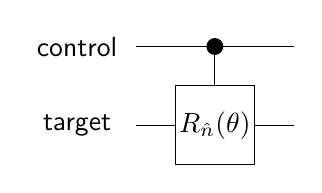
\begin{tikzpicture}[scale=.5] \node[draw=none] at (-3.5, 2) {control}; \node[draw=none] at (-3.5, 0) {target}; \draw (-2, 2) -- (2, 2); \draw[fill=black] (0, 2) circle (.2); \draw (0, 2) -- (0, 1); \draw (-2,0) -- (-1, 0); \draw (1, 0) -- (2, 0); \draw (-1,-1)--(-1,1)--(1,1)--(1,-1)--cycle; \node[draw=none] at (0, 0) {$R_{\hat{n}}(\theta)$}; \end{tikzpicture} } \]


\begin{DoxyParams}[1]{Parameters}
\mbox{\tt in,out}  & {\em multi\+Qubit} & object representing the set of all qubits \\
\hline
\mbox{\tt in}  & {\em control\+Qubit} & qubit with value 1 in the rotated states \\
\hline
\mbox{\tt in}  & {\em target\+Qubit} & qubit to rotate \\
\hline
\mbox{\tt in}  & {\em angle} & angle by which to rotate in radians \\
\hline
\mbox{\tt in}  & {\em axis} & vector around which to rotate (can be non-\/unit; will be normalised) \\
\hline
\end{DoxyParams}

\begin{DoxyExceptions}{Exceptions}
{\em exit\+With\+Error} & if either {\ttfamily control\+Qubit} or {\ttfamily target\+Qubit} are outside \mbox{[}0, {\ttfamily multi\+Qubit.\+num\+Qubits}) or are equal or if {\ttfamily axis} is the zero vector \\
\hline
\end{DoxyExceptions}


Definition at line 138 of file Qu\+E\+S\+T.\+cpp.



References controlled\+Compact\+Unitary(), Complex\+::imag, Complex\+::real, Vector\+::x, Vector\+::y, and Vector\+::z.



Referenced by controlled\+Rotate\+X(), controlled\+Rotate\+Y(), and controlled\+Rotate\+Z().


\begin{DoxyCode}
138                                                                                                            
                         \{
139 
140     \textcolor{keywordtype}{double} mag = sqrt(pow(axis.\mbox{\hyperlink{structVector_aac7abe171ba4bada50ed72acba6259fc}{x}},2) + pow(axis.\mbox{\hyperlink{structVector_a375ca805d4c808a53d7c4e0c737ae3de}{y}},2) + pow(axis.\mbox{\hyperlink{structVector_ad4e863651be7d6b7e2b28cd7445a0ccf}{z}},2));
141     \mbox{\hyperlink{structVector}{Vector}} unitAxis = \{axis.\mbox{\hyperlink{structVector_aac7abe171ba4bada50ed72acba6259fc}{x}}/mag, axis.\mbox{\hyperlink{structVector_a375ca805d4c808a53d7c4e0c737ae3de}{y}}/mag, axis.\mbox{\hyperlink{structVector_ad4e863651be7d6b7e2b28cd7445a0ccf}{z}}/mag\};
142 
143     \mbox{\hyperlink{structComplex}{Complex}} alpha, beta;
144     alpha.\mbox{\hyperlink{structComplex_a479ad939835457595fcca3ca55c06283}{real}} = cos(angle/2.0);
145     alpha.\mbox{\hyperlink{structComplex_a1151948284b21c0052f203f23ab931d9}{imag}} = -sin(angle/2.0)*unitAxis.\mbox{\hyperlink{structVector_ad4e863651be7d6b7e2b28cd7445a0ccf}{z}};    
146     beta.\mbox{\hyperlink{structComplex_a479ad939835457595fcca3ca55c06283}{real}} = sin(angle/2.0)*unitAxis.\mbox{\hyperlink{structVector_a375ca805d4c808a53d7c4e0c737ae3de}{y}};
147     beta.\mbox{\hyperlink{structComplex_a1151948284b21c0052f203f23ab931d9}{imag}} = -sin(angle/2.0)*unitAxis.\mbox{\hyperlink{structVector_aac7abe171ba4bada50ed72acba6259fc}{x}};
148     \mbox{\hyperlink{QuEST_8h_ab4812953bc457405b3aa05a4c2f64f4a}{controlledCompactUnitary}}(multiQubit, controlQubit, targetQubit, alpha, beta);
149 \}
\end{DoxyCode}
\mbox{\Hypertarget{QuEST_8cpp_ac6923ac57e67d9a21096e06f6a9012f6}\label{QuEST_8cpp_ac6923ac57e67d9a21096e06f6a9012f6}} 
\index{Qu\+E\+S\+T.\+cpp@{Qu\+E\+S\+T.\+cpp}!controlled\+RotateX@{controlled\+RotateX}}
\index{controlled\+RotateX@{controlled\+RotateX}!Qu\+E\+S\+T.\+cpp@{Qu\+E\+S\+T.\+cpp}}
\paragraph{\texorpdfstring{controlled\+Rotate\+X()}{controlledRotateX()}}
{\footnotesize\ttfamily void controlled\+RotateX (\begin{DoxyParamCaption}\item[{\mbox{\hyperlink{structMultiQubit}{Multi\+Qubit}}}]{multi\+Qubit,  }\item[{const int}]{control\+Qubit,  }\item[{const int}]{target\+Qubit,  }\item[{\mbox{\hyperlink{QuEST__precision_8h_a4b654506f18b8bfd61ad2a29a7e38c25}{R\+E\+AL}}}]{angle }\end{DoxyParamCaption})}



Applies a controlled rotation by a given angle around the X-\/axis of the Bloch-\/sphere. 

The target qubit is rotated in states where the control qubit has value 1.

\[ \setlength{\fboxrule}{0.01pt} \fbox{ 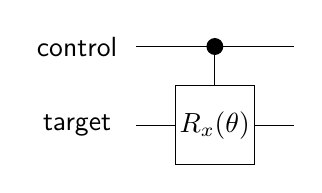
\begin{tikzpicture}[scale=.5] \node[draw=none] at (-3.5, 2) {control}; \node[draw=none] at (-3.5, 0) {target}; \draw (-2, 2) -- (2, 2); \draw[fill=black] (0, 2) circle (.2); \draw (0, 2) -- (0, 1); \draw (-2,0) -- (-1, 0); \draw (1, 0) -- (2, 0); \draw (-1,-1)--(-1,1)--(1,1)--(1,-1)--cycle; \node[draw=none] at (0, 0) {$R_x(\theta)$}; \end{tikzpicture} } \] ~\newline
 
\begin{DoxyParams}[1]{Parameters}
\mbox{\tt in,out}  & {\em multi\+Qubit} & object representing the set of all qubits \\
\hline
\mbox{\tt in}  & {\em control\+Qubit} & qubit which has value 1 in the rotated states \\
\hline
\mbox{\tt in}  & {\em tagret\+Qubit} & qubit to rotate \\
\hline
\mbox{\tt in}  & {\em angle} & angle by which to rotate the target qubit in radians \\
\hline
\end{DoxyParams}

\begin{DoxyExceptions}{Exceptions}
{\em exit\+With\+Error} & if either {\ttfamily control\+Qubit} or {\ttfamily target\+Qubit} are outside \mbox{[}0, {\ttfamily multi\+Qubit.\+num\+Qubits}) or are equal. \\
\hline
\end{DoxyExceptions}


Definition at line 151 of file Qu\+E\+S\+T.\+cpp.



References controlled\+Rotate\+Around\+Axis().


\begin{DoxyCode}
151                                                                                                         \{
152 
153     \mbox{\hyperlink{structVector}{Vector}} unitAxis = \{1, 0, 0\};
154     \mbox{\hyperlink{QuEST_8cpp_ad41f82b41149393a642391b67b3a287e}{controlledRotateAroundAxis}}(multiQubit, controlQubit, targetQubit, angle, 
      unitAxis);
155 \}
\end{DoxyCode}
\mbox{\Hypertarget{QuEST_8cpp_a71e90a2f7292116338c062934f9d1202}\label{QuEST_8cpp_a71e90a2f7292116338c062934f9d1202}} 
\index{Qu\+E\+S\+T.\+cpp@{Qu\+E\+S\+T.\+cpp}!controlled\+RotateY@{controlled\+RotateY}}
\index{controlled\+RotateY@{controlled\+RotateY}!Qu\+E\+S\+T.\+cpp@{Qu\+E\+S\+T.\+cpp}}
\paragraph{\texorpdfstring{controlled\+Rotate\+Y()}{controlledRotateY()}}
{\footnotesize\ttfamily void controlled\+RotateY (\begin{DoxyParamCaption}\item[{\mbox{\hyperlink{structMultiQubit}{Multi\+Qubit}}}]{multi\+Qubit,  }\item[{const int}]{control\+Qubit,  }\item[{const int}]{target\+Qubit,  }\item[{\mbox{\hyperlink{QuEST__precision_8h_a4b654506f18b8bfd61ad2a29a7e38c25}{R\+E\+AL}}}]{angle }\end{DoxyParamCaption})}



Applies a controlled rotation by a given angle around the Y-\/axis of the Bloch-\/sphere. 

The target qubit is rotated in states where the control qubit has value 1.

\[ \setlength{\fboxrule}{0.01pt} \fbox{ 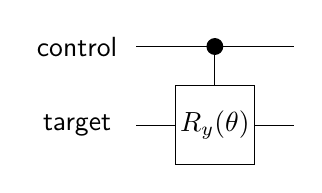
\begin{tikzpicture}[scale=.5] \node[draw=none] at (-3.5, 2) {control}; \node[draw=none] at (-3.5, 0) {target}; \draw (-2, 2) -- (2, 2); \draw[fill=black] (0, 2) circle (.2); \draw (0, 2) -- (0, 1); \draw (-2,0) -- (-1, 0); \draw (1, 0) -- (2, 0); \draw (-1,-1)--(-1,1)--(1,1)--(1,-1)--cycle; \node[draw=none] at (0, 0) {$R_y(\theta)$}; \end{tikzpicture} } \] ~\newline
 
\begin{DoxyParams}[1]{Parameters}
\mbox{\tt in,out}  & {\em multi\+Qubit} & object representing the set of all qubits \\
\hline
\mbox{\tt in}  & {\em control\+Qubit} & qubit which has value 1 in the rotated states \\
\hline
\mbox{\tt in}  & {\em tagret\+Qubit} & qubit to rotate \\
\hline
\mbox{\tt in}  & {\em angle} & angle by which to rotate the target qubit in radians \\
\hline
\end{DoxyParams}

\begin{DoxyExceptions}{Exceptions}
{\em exit\+With\+Error} & if either {\ttfamily control\+Qubit} or {\ttfamily target\+Qubit} are outside \mbox{[}0, {\ttfamily multi\+Qubit.\+num\+Qubits}) or are equal. \\
\hline
\end{DoxyExceptions}


Definition at line 157 of file Qu\+E\+S\+T.\+cpp.



References controlled\+Rotate\+Around\+Axis().


\begin{DoxyCode}
157                                                                                                         \{
158 
159     \mbox{\hyperlink{structVector}{Vector}} unitAxis = \{0, 1, 0\};
160     \mbox{\hyperlink{QuEST_8cpp_ad41f82b41149393a642391b67b3a287e}{controlledRotateAroundAxis}}(multiQubit, controlQubit, targetQubit, angle, 
      unitAxis);
161 \}
\end{DoxyCode}
\mbox{\Hypertarget{QuEST_8cpp_a668e5d2634b02e98bc73675ccb11d61c}\label{QuEST_8cpp_a668e5d2634b02e98bc73675ccb11d61c}} 
\index{Qu\+E\+S\+T.\+cpp@{Qu\+E\+S\+T.\+cpp}!controlled\+RotateZ@{controlled\+RotateZ}}
\index{controlled\+RotateZ@{controlled\+RotateZ}!Qu\+E\+S\+T.\+cpp@{Qu\+E\+S\+T.\+cpp}}
\paragraph{\texorpdfstring{controlled\+Rotate\+Z()}{controlledRotateZ()}}
{\footnotesize\ttfamily void controlled\+RotateZ (\begin{DoxyParamCaption}\item[{\mbox{\hyperlink{structMultiQubit}{Multi\+Qubit}}}]{multi\+Qubit,  }\item[{const int}]{control\+Qubit,  }\item[{const int}]{target\+Qubit,  }\item[{\mbox{\hyperlink{QuEST__precision_8h_a4b654506f18b8bfd61ad2a29a7e38c25}{R\+E\+AL}}}]{angle }\end{DoxyParamCaption})}



Applies a controlled rotation by a given angle around the Z-\/axis of the Bloch-\/sphere. 

The target qubit is rotated in states where the control qubit has value 1.

\[ \setlength{\fboxrule}{0.01pt} \fbox{ 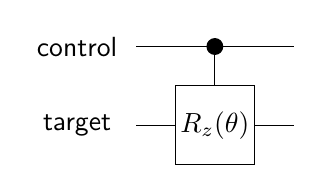
\begin{tikzpicture}[scale=.5] \node[draw=none] at (-3.5, 2) {control}; \node[draw=none] at (-3.5, 0) {target}; \draw (-2, 2) -- (2, 2); \draw[fill=black] (0, 2) circle (.2); \draw (0, 2) -- (0, 1); \draw (-2,0) -- (-1, 0); \draw (1, 0) -- (2, 0); \draw (-1,-1)--(-1,1)--(1,1)--(1,-1)--cycle; \node[draw=none] at (0, 0) {$R_z(\theta)$}; \end{tikzpicture} } \] ~\newline
 
\begin{DoxyParams}[1]{Parameters}
\mbox{\tt in,out}  & {\em multi\+Qubit} & object representing the set of all qubits \\
\hline
\mbox{\tt in}  & {\em control\+Qubit} & qubit which has value 1 in the rotated states \\
\hline
\mbox{\tt in}  & {\em tagret\+Qubit} & qubit to rotate \\
\hline
\mbox{\tt in}  & {\em angle} & angle by which to rotate the target qubit in radians \\
\hline
\end{DoxyParams}

\begin{DoxyExceptions}{Exceptions}
{\em exit\+With\+Error} & if either {\ttfamily control\+Qubit} or {\ttfamily target\+Qubit} are outside \mbox{[}0, {\ttfamily multi\+Qubit.\+num\+Qubits}) or are equal. \\
\hline
\end{DoxyExceptions}


Definition at line 163 of file Qu\+E\+S\+T.\+cpp.



References controlled\+Rotate\+Around\+Axis().


\begin{DoxyCode}
163                                                                                                         \{
164 
165     \mbox{\hyperlink{structVector}{Vector}} unitAxis = \{0, 0, 1\};
166     \mbox{\hyperlink{QuEST_8cpp_ad41f82b41149393a642391b67b3a287e}{controlledRotateAroundAxis}}(multiQubit, controlQubit, targetQubit, angle, 
      unitAxis);
167 \}
\end{DoxyCode}
\mbox{\Hypertarget{QuEST_8cpp_ac61ecf4fd9ab2ac8453c4eb5b0d34089}\label{QuEST_8cpp_ac61ecf4fd9ab2ac8453c4eb5b0d34089}} 
\index{Qu\+E\+S\+T.\+cpp@{Qu\+E\+S\+T.\+cpp}!get\+Num\+Amps@{get\+Num\+Amps}}
\index{get\+Num\+Amps@{get\+Num\+Amps}!Qu\+E\+S\+T.\+cpp@{Qu\+E\+S\+T.\+cpp}}
\paragraph{\texorpdfstring{get\+Num\+Amps()}{getNumAmps()}}
{\footnotesize\ttfamily int get\+Num\+Amps (\begin{DoxyParamCaption}\item[{\mbox{\hyperlink{structMultiQubit}{Multi\+Qubit}}}]{multi\+Qubit }\end{DoxyParamCaption})}



Get the number of probability amplitudes in a multi\+Qubit object, given by 2$^\wedge$num\+Qubits. 



Definition at line 95 of file Qu\+E\+S\+T.\+cpp.



References Multi\+Qubit\+::num\+Amps\+Divided\+By\+Num\+Chunks, and Multi\+Qubit\+::num\+Chunks.


\begin{DoxyCode}
95                                      \{
96     \textcolor{keywordflow}{return} multiQubit.\mbox{\hyperlink{structMultiQubit_a04c9f5254af58e4c4a54712eb32e7082}{numAmpsDividedByNumChunks}}*multiQubit.
      \mbox{\hyperlink{structMultiQubit_acd43f2f57991709c9e94f73662c972b2}{numChunks}};
97 \}
\end{DoxyCode}
\mbox{\Hypertarget{QuEST_8cpp_a00e13dc88021b61a29fac9f3ab9ee850}\label{QuEST_8cpp_a00e13dc88021b61a29fac9f3ab9ee850}} 
\index{Qu\+E\+S\+T.\+cpp@{Qu\+E\+S\+T.\+cpp}!get\+Num\+Qubits@{get\+Num\+Qubits}}
\index{get\+Num\+Qubits@{get\+Num\+Qubits}!Qu\+E\+S\+T.\+cpp@{Qu\+E\+S\+T.\+cpp}}
\paragraph{\texorpdfstring{get\+Num\+Qubits()}{getNumQubits()}}
{\footnotesize\ttfamily int get\+Num\+Qubits (\begin{DoxyParamCaption}\item[{\mbox{\hyperlink{structMultiQubit}{Multi\+Qubit}}}]{multi\+Qubit }\end{DoxyParamCaption})}



Rotate a single qubit by a given angle around a given vector on the Bloch-\/sphere. 


\begin{DoxyItemize}
\item The vector must not be zero (else an error is thrown), but needn\textquotesingle{}t be unit magnitude.
\end{DoxyItemize}


\begin{DoxyParams}[1]{Parameters}
\mbox{\tt in,out}  & {\em multi\+Qubit} & object representing the set of all qubits \\
\hline
\mbox{\tt in}  & {\em rot\+Qubit} & qubit to rotate \\
\hline
\mbox{\tt in}  & {\em angle} & angle by which to rotate in radians \\
\hline
\mbox{\tt in}  & {\em axis} & vector around which to rotate \\
\hline
\end{DoxyParams}

\begin{DoxyExceptions}{Exceptions}
{\em exit\+With\+Error} & if {\ttfamily rot\+Qubit} is outside \mbox{[}0, {\ttfamily multi\+Qubit.\+num\+Qubits}), or if {\ttfamily axis} is the zero vector\+Get the number of qubits in a multi\+Qubit object \\
\hline
\end{DoxyExceptions}


Definition at line 91 of file Qu\+E\+S\+T.\+cpp.



References Multi\+Qubit\+::num\+Qubits.


\begin{DoxyCode}
91                                        \{
92     \textcolor{keywordflow}{return} multiQubit.\mbox{\hyperlink{structMultiQubit_ab5b9795bdc6fb5855e1974dcbbaeb36f}{numQubits}};
93 \}
\end{DoxyCode}
\mbox{\Hypertarget{QuEST_8cpp_a799b10447d6dbdaf960a4d3eedd22014}\label{QuEST_8cpp_a799b10447d6dbdaf960a4d3eedd22014}} 
\index{Qu\+E\+S\+T.\+cpp@{Qu\+E\+S\+T.\+cpp}!get\+Prob\+El@{get\+Prob\+El}}
\index{get\+Prob\+El@{get\+Prob\+El}!Qu\+E\+S\+T.\+cpp@{Qu\+E\+S\+T.\+cpp}}
\paragraph{\texorpdfstring{get\+Prob\+El()}{getProbEl()}}
{\footnotesize\ttfamily \mbox{\hyperlink{QuEST__precision_8h_a4b654506f18b8bfd61ad2a29a7e38c25}{R\+E\+AL}} get\+Prob\+El (\begin{DoxyParamCaption}\item[{\mbox{\hyperlink{structMultiQubit}{Multi\+Qubit}}}]{multi\+Qubit,  }\item[{long long int}]{index }\end{DoxyParamCaption})}



Get the probability of the state at an index in the full state vector. 


\begin{DoxyParams}[1]{Parameters}
\mbox{\tt in}  & {\em multi\+Qubit} & object representing a set of qubits \\
\hline
\mbox{\tt in}  & {\em index} & index in state vector of probability amplitudes \\
\hline
\end{DoxyParams}
\begin{DoxyReturn}{Returns}
real\+El$\ast$real\+El + imag\+El$\ast$imag\+El 
\end{DoxyReturn}

\begin{DoxyExceptions}{Exceptions}
{\em exit\+With\+Error} & if {\ttfamily index} is outside \mbox{[}0, $2^{N}$) where $N = $ {\ttfamily multi\+Qubit.\+num\+Qubits} \\
\hline
\end{DoxyExceptions}


Definition at line 99 of file Qu\+E\+S\+T.\+cpp.



References get\+Imag\+Amp\+El(), get\+Real\+Amp\+El(), and R\+E\+AL.


\begin{DoxyCode}
99                                                           \{
100     \mbox{\hyperlink{QuEST__precision_8h_a4b654506f18b8bfd61ad2a29a7e38c25}{REAL}} real;
101     \mbox{\hyperlink{QuEST__precision_8h_a4b654506f18b8bfd61ad2a29a7e38c25}{REAL}} imag;
102     real = \mbox{\hyperlink{QuEST_8h_a317b786f577fa6bc136ea7f0ee7330a7}{getRealAmpEl}}(multiQubit, index);
103     imag = \mbox{\hyperlink{QuEST_8h_a3615f76fd5f57008d9b74bbd10533dd0}{getImagAmpEl}}(multiQubit, index);
104     \textcolor{keywordflow}{return} real*real + imag*imag;
105 \}
\end{DoxyCode}
\mbox{\Hypertarget{QuEST_8cpp_ab76254cfde16f0808476649507a1a2fc}\label{QuEST_8cpp_ab76254cfde16f0808476649507a1a2fc}} 
\index{Qu\+E\+S\+T.\+cpp@{Qu\+E\+S\+T.\+cpp}!hash\+String@{hash\+String}}
\index{hash\+String@{hash\+String}!Qu\+E\+S\+T.\+cpp@{Qu\+E\+S\+T.\+cpp}}
\paragraph{\texorpdfstring{hash\+String()}{hashString()}}
{\footnotesize\ttfamily unsigned long int hash\+String (\begin{DoxyParamCaption}\item[{char $\ast$}]{str }\end{DoxyParamCaption})}



Definition at line 254 of file Qu\+E\+S\+T.\+cpp.



Referenced by Qu\+E\+S\+T\+Seed\+Random\+Default().


\begin{DoxyCode}
254                                        \{
255     \textcolor{keywordtype}{unsigned} \textcolor{keywordtype}{long} \textcolor{keywordtype}{int} hash = 5381;
256     \textcolor{keywordtype}{int} c;
257 
258     \textcolor{keywordflow}{while} ((c = *str++))
259         hash = ((hash << 5) + hash) + c; \textcolor{comment}{/* hash * 33 + c */}
260 
261     \textcolor{keywordflow}{return} hash;    
262 \}
\end{DoxyCode}
\mbox{\Hypertarget{QuEST_8cpp_aedb5ef39da69e7895d714980dc621261}\label{QuEST_8cpp_aedb5ef39da69e7895d714980dc621261}} 
\index{Qu\+E\+S\+T.\+cpp@{Qu\+E\+S\+T.\+cpp}!Qu\+E\+S\+T\+Seed\+Random@{Qu\+E\+S\+T\+Seed\+Random}}
\index{Qu\+E\+S\+T\+Seed\+Random@{Qu\+E\+S\+T\+Seed\+Random}!Qu\+E\+S\+T.\+cpp@{Qu\+E\+S\+T.\+cpp}}
\paragraph{\texorpdfstring{Qu\+E\+S\+T\+Seed\+Random()}{QuESTSeedRandom()}}
{\footnotesize\ttfamily void Qu\+E\+S\+T\+Seed\+Random (\begin{DoxyParamCaption}\item[{unsigned long int $\ast$}]{seed\+Array,  }\item[{int}]{num\+Seeds }\end{DoxyParamCaption})}



num\+Seeds $<$= 64 

Seed the Mersenne Twister used for random number generation in the Qu\+E\+ST environment with a user defined seed. 

Definition at line 247 of file Qu\+E\+S\+T.\+cpp.



References init\+\_\+by\+\_\+array().


\begin{DoxyCode}
247                                                                 \{
248     \textcolor{comment}{// init MT random number generator with user defined list of seeds}
249     \textcolor{comment}{// for the MPI version, it is ok that all procs will get the same seed as random numbers will only be }
250     \textcolor{comment}{// used by the master process}
251     \mbox{\hyperlink{mt19937ar_8cpp_ac1283f9b1ed571332f5ffe53545ffc16}{init\_by\_array}}(seedArray, numSeeds); 
252 \}
\end{DoxyCode}
\mbox{\Hypertarget{QuEST_8cpp_a30b2a5228b8a21419db8aa82fa5e3167}\label{QuEST_8cpp_a30b2a5228b8a21419db8aa82fa5e3167}} 
\index{Qu\+E\+S\+T.\+cpp@{Qu\+E\+S\+T.\+cpp}!Qu\+E\+S\+T\+Seed\+Random\+Default@{Qu\+E\+S\+T\+Seed\+Random\+Default}}
\index{Qu\+E\+S\+T\+Seed\+Random\+Default@{Qu\+E\+S\+T\+Seed\+Random\+Default}!Qu\+E\+S\+T.\+cpp@{Qu\+E\+S\+T.\+cpp}}
\paragraph{\texorpdfstring{Qu\+E\+S\+T\+Seed\+Random\+Default()}{QuESTSeedRandomDefault()}}
{\footnotesize\ttfamily void Qu\+E\+S\+T\+Seed\+Random\+Default (\begin{DoxyParamCaption}\item[{void}]{ }\end{DoxyParamCaption})}



Seed the Mersenne Twister used for random number generation in the Qu\+E\+ST environment with an example defualt seed. 

This default seeding function uses the mt19937 init\+\_\+by\+\_\+array function with three keys -- time, pid and hostname. Subsequent calls to mt19937 genrand functions will use this seeding. For a multi process code, the same seed is given to all process, therefore this seeding is only appropriate to use for functions such as measure where all processes require the same random value.

For more information about the MT, see \href{http://www.math.sci.hiroshima-u.ac.jp/~m-mat/MT/MT2002/emt19937ar.html}{\tt http\+://www.\+math.\+sci.\+hiroshima-\/u.\+ac.\+jp/$\sim$m-\/mat/\+M\+T/\+M\+T2002/emt19937ar.\+html} 

Definition at line 222 of file Qu\+E\+S\+T.\+cpp.



References hash\+String(), and init\+\_\+by\+\_\+array().


\begin{DoxyCode}
222                              \{
223     \textcolor{comment}{// init MT random number generator with three keys -- time, pid and a hash of hostname }
224     \textcolor{comment}{// for the MPI version, it is ok that all procs will get the same seed as random numbers will only be }
225     \textcolor{comment}{// used by the master process}
226 
227     \textcolor{keyword}{struct }timeval  tv;
228     gettimeofday(&tv, NULL);
229 
230     \textcolor{keywordtype}{double} time\_in\_mill = 
231         (tv.tv\_sec) * 1000 + (tv.tv\_usec) / 1000 ; \textcolor{comment}{// convert tv\_sec & tv\_usec to millisecond}
232 
233     \textcolor{keywordtype}{unsigned} \textcolor{keywordtype}{long} \textcolor{keywordtype}{int} pid = getpid();
234     \textcolor{keywordtype}{unsigned} \textcolor{keywordtype}{long} \textcolor{keywordtype}{int} msecs = (\textcolor{keywordtype}{unsigned} \textcolor{keywordtype}{long} int) time\_in\_mill;
235     \textcolor{keywordtype}{char} hostName[MAXHOSTNAMELEN+1];
236     gethostname(hostName, \textcolor{keyword}{sizeof}(hostName));
237     \textcolor{keywordtype}{unsigned} \textcolor{keywordtype}{long} \textcolor{keywordtype}{int} hostNameInt = \mbox{\hyperlink{QuEST_8cpp_ab76254cfde16f0808476649507a1a2fc}{hashString}}(hostName);
238 
239     \textcolor{keywordtype}{unsigned} \textcolor{keywordtype}{long} \textcolor{keywordtype}{int} key[3];
240     key[0] = msecs; key[1] = pid; key[2] = hostNameInt;
241     \mbox{\hyperlink{mt19937ar_8cpp_ac1283f9b1ed571332f5ffe53545ffc16}{init\_by\_array}}(key, 3); 
242 \}
\end{DoxyCode}
\mbox{\Hypertarget{QuEST_8cpp_aa5e77e0e64f3a4a3d3f5cc7382bffcd9}\label{QuEST_8cpp_aa5e77e0e64f3a4a3d3f5cc7382bffcd9}} 
\index{Qu\+E\+S\+T.\+cpp@{Qu\+E\+S\+T.\+cpp}!report\+Multi\+Qubit\+Params@{report\+Multi\+Qubit\+Params}}
\index{report\+Multi\+Qubit\+Params@{report\+Multi\+Qubit\+Params}!Qu\+E\+S\+T.\+cpp@{Qu\+E\+S\+T.\+cpp}}
\paragraph{\texorpdfstring{report\+Multi\+Qubit\+Params()}{reportMultiQubitParams()}}
{\footnotesize\ttfamily void report\+Multi\+Qubit\+Params (\begin{DoxyParamCaption}\item[{\mbox{\hyperlink{structMultiQubit}{Multi\+Qubit}}}]{multi\+Qubit }\end{DoxyParamCaption})}



Report metainformation about a set of qubits\+: number of qubits, number of probability amplitudes. 


\begin{DoxyParams}[1]{Parameters}
\mbox{\tt in,out}  & {\em multi\+Qubit} & object representing the set of qubits \\
\hline
\mbox{\tt in}  & {\em env} & object representing the execution environment (local, multinode etc) \\
\hline
\end{DoxyParams}


Definition at line 80 of file Qu\+E\+S\+T.\+cpp.



References Multi\+Qubit\+::chunk\+Id, Multi\+Qubit\+::num\+Chunks, and Multi\+Qubit\+::num\+Qubits.


\begin{DoxyCode}
80                                                   \{
81         \textcolor{keywordtype}{long} \textcolor{keywordtype}{long} \textcolor{keywordtype}{int} numAmps = 1L << multiQubit.\mbox{\hyperlink{structMultiQubit_ab5b9795bdc6fb5855e1974dcbbaeb36f}{numQubits}};
82         \textcolor{keywordtype}{long} \textcolor{keywordtype}{long} \textcolor{keywordtype}{int} numAmpsPerRank = numAmps/multiQubit.\mbox{\hyperlink{structMultiQubit_acd43f2f57991709c9e94f73662c972b2}{numChunks}};
83         \textcolor{keywordflow}{if} (multiQubit.\mbox{\hyperlink{structMultiQubit_ab10c88249fa3825d6227ceec01d37e37}{chunkId}}==0)\{
84                 printf(\textcolor{stringliteral}{"QUBITS:\(\backslash\)n"});
85                 printf(\textcolor{stringliteral}{"Number of qubits is %d.\(\backslash\)n"}, multiQubit.\mbox{\hyperlink{structMultiQubit_ab5b9795bdc6fb5855e1974dcbbaeb36f}{numQubits}});
86                 printf(\textcolor{stringliteral}{"Number of amps is %lld.\(\backslash\)n"}, numAmps);
87                 printf(\textcolor{stringliteral}{"Number of amps per rank is %lld.\(\backslash\)n"}, numAmpsPerRank);
88     \}
89 \}
\end{DoxyCode}
\mbox{\Hypertarget{QuEST_8cpp_a96f4de9ce7fefc7680a44d601fc3d894}\label{QuEST_8cpp_a96f4de9ce7fefc7680a44d601fc3d894}} 
\index{Qu\+E\+S\+T.\+cpp@{Qu\+E\+S\+T.\+cpp}!report\+State@{report\+State}}
\index{report\+State@{report\+State}!Qu\+E\+S\+T.\+cpp@{Qu\+E\+S\+T.\+cpp}}
\paragraph{\texorpdfstring{report\+State()}{reportState()}}
{\footnotesize\ttfamily void report\+State (\begin{DoxyParamCaption}\item[{\mbox{\hyperlink{structMultiQubit}{Multi\+Qubit}}}]{multi\+Qubit }\end{DoxyParamCaption})}



Print the current state vector of probability amplitudes for a set of qubits to file. 

File format\+: \begin{DoxyVerb}real, imag
realComponent1, imagComponent1
realComponent2, imagComponent2
...
realComponentN, imagComponentN
\end{DoxyVerb}


File naming convention\+:

For each node that the program runs on, a file \textquotesingle{}state\+\_\+rank\+\_\+\mbox{[}node\+\_\+rank\mbox{]}.csv\textquotesingle{} is generated. If there is more than one node, ranks after the first do not include the header \begin{DoxyVerb}real, imag
\end{DoxyVerb}
 so that files are easier to combine. 
\begin{DoxyParams}[1]{Parameters}
\mbox{\tt in,out}  & {\em multi\+Qubit} & object representing the set of qubits \\
\hline
\end{DoxyParams}


Definition at line 62 of file Qu\+E\+S\+T.\+cpp.



References Multi\+Qubit\+::chunk\+Id, Complex\+Array\+::imag, Multi\+Qubit\+::num\+Amps\+Divided\+By\+Num\+Chunks, Complex\+Array\+::real, and Multi\+Qubit\+::state\+Vec.


\begin{DoxyCode}
62                                        \{
63         FILE *state;
64         \textcolor{keywordtype}{char} filename[100];
65         \textcolor{keywordtype}{long} \textcolor{keywordtype}{long} \textcolor{keywordtype}{int} index;
66         sprintf(filename, \textcolor{stringliteral}{"state\_rank\_%d.csv"}, multiQubit.\mbox{\hyperlink{structMultiQubit_ab10c88249fa3825d6227ceec01d37e37}{chunkId}});
67         state = fopen(filename, \textcolor{stringliteral}{"w"});
68         \textcolor{keywordflow}{if} (multiQubit.\mbox{\hyperlink{structMultiQubit_ab10c88249fa3825d6227ceec01d37e37}{chunkId}}==0) fprintf(state, \textcolor{stringliteral}{"real, imag\(\backslash\)n"});
69 
70         \textcolor{keywordflow}{for}(index=0; index<multiQubit.\mbox{\hyperlink{structMultiQubit_a04c9f5254af58e4c4a54712eb32e7082}{numAmpsDividedByNumChunks}}; index++)\{
71                 fprintf(state, \textcolor{stringliteral}{"%.12f, %.12f\(\backslash\)n"}, multiQubit.\mbox{\hyperlink{structMultiQubit_a45483190d6b01ef6b2f98f2bec9ab94f}{stateVec}}.
      \mbox{\hyperlink{structComplexArray_a4195cac6c784ea1b6271f1c7dba1548a}{real}}[index], multiQubit.\mbox{\hyperlink{structMultiQubit_a45483190d6b01ef6b2f98f2bec9ab94f}{stateVec}}.\mbox{\hyperlink{structComplexArray_a79dde47c7ae530c79cebfdf57b225968}{imag}}[index]);
72         \}
73         fclose(state);
74 \}
\end{DoxyCode}
\mbox{\Hypertarget{QuEST_8cpp_a8810423457803005fecd415f4299f40d}\label{QuEST_8cpp_a8810423457803005fecd415f4299f40d}} 
\index{Qu\+E\+S\+T.\+cpp@{Qu\+E\+S\+T.\+cpp}!rotate\+Around\+Axis@{rotate\+Around\+Axis}}
\index{rotate\+Around\+Axis@{rotate\+Around\+Axis}!Qu\+E\+S\+T.\+cpp@{Qu\+E\+S\+T.\+cpp}}
\paragraph{\texorpdfstring{rotate\+Around\+Axis()}{rotateAroundAxis()}}
{\footnotesize\ttfamily void rotate\+Around\+Axis (\begin{DoxyParamCaption}\item[{\mbox{\hyperlink{structMultiQubit}{Multi\+Qubit}}}]{multi\+Qubit,  }\item[{const int}]{rot\+Qubit,  }\item[{\mbox{\hyperlink{QuEST__precision_8h_a4b654506f18b8bfd61ad2a29a7e38c25}{R\+E\+AL}}}]{angle,  }\item[{\mbox{\hyperlink{structVector}{Vector}}}]{unit\+Axis }\end{DoxyParamCaption})}



Rotate a single qubit by a given angle around a given vector on the Bloch-\/sphere. 

The vector must not be zero (else an error is thrown), but needn\textquotesingle{}t be unit magnitude.

For angle $\theta$ and axis vector $\vec{n}$, applies $R_{\hat{n}} = \exp \left(- i \frac{\theta}{2} \hat{n} \cdot \vec{\sigma} \right) $ where $\vec{\sigma}$ is the vector of Pauli matrices.


\begin{DoxyParams}[1]{Parameters}
\mbox{\tt in,out}  & {\em multi\+Qubit} & object representing the set of all qubits \\
\hline
\mbox{\tt in}  & {\em rot\+Qubit} & qubit to rotate \\
\hline
\mbox{\tt in}  & {\em angle} & angle by which to rotate in radians \\
\hline
\mbox{\tt in}  & {\em axis} & vector around which to rotate (can be non-\/unit; will be normalised) \\
\hline
\end{DoxyParams}

\begin{DoxyExceptions}{Exceptions}
{\em exit\+With\+Error} & if {\ttfamily rot\+Qubit} is outside \mbox{[}0, {\ttfamily multi\+Qubit.\+num\+Qubits}), or if {\ttfamily axis} is the zero vector \\
\hline
\end{DoxyExceptions}


Definition at line 107 of file Qu\+E\+S\+T.\+cpp.



References compact\+Unitary(), Complex\+::imag, Complex\+::real, Vector\+::x, Vector\+::y, and Vector\+::z.



Referenced by rotate\+X(), rotate\+Y(), and rotate\+Z().


\begin{DoxyCode}
107                                                                                          \{
108 
109     \textcolor{keywordtype}{double} mag = sqrt(pow(axis.\mbox{\hyperlink{structVector_aac7abe171ba4bada50ed72acba6259fc}{x}},2) + pow(axis.\mbox{\hyperlink{structVector_a375ca805d4c808a53d7c4e0c737ae3de}{y}},2) + pow(axis.\mbox{\hyperlink{structVector_ad4e863651be7d6b7e2b28cd7445a0ccf}{z}},2));
110     \mbox{\hyperlink{structVector}{Vector}} unitAxis = \{axis.\mbox{\hyperlink{structVector_aac7abe171ba4bada50ed72acba6259fc}{x}}/mag, axis.\mbox{\hyperlink{structVector_a375ca805d4c808a53d7c4e0c737ae3de}{y}}/mag, axis.\mbox{\hyperlink{structVector_ad4e863651be7d6b7e2b28cd7445a0ccf}{z}}/mag\};
111 
112     \mbox{\hyperlink{structComplex}{Complex}} alpha, beta;
113     alpha.\mbox{\hyperlink{structComplex_a479ad939835457595fcca3ca55c06283}{real}} = cos(angle/2.0);
114     alpha.\mbox{\hyperlink{structComplex_a1151948284b21c0052f203f23ab931d9}{imag}} = -sin(angle/2.0)*unitAxis.\mbox{\hyperlink{structVector_ad4e863651be7d6b7e2b28cd7445a0ccf}{z}};    
115     beta.\mbox{\hyperlink{structComplex_a479ad939835457595fcca3ca55c06283}{real}} = sin(angle/2.0)*unitAxis.\mbox{\hyperlink{structVector_a375ca805d4c808a53d7c4e0c737ae3de}{y}};
116     beta.\mbox{\hyperlink{structComplex_a1151948284b21c0052f203f23ab931d9}{imag}} = -sin(angle/2.0)*unitAxis.\mbox{\hyperlink{structVector_aac7abe171ba4bada50ed72acba6259fc}{x}};
117     \mbox{\hyperlink{QuEST_8h_ad13ae1902276195d0df106116e032aff}{compactUnitary}}(multiQubit, rotQubit, alpha, beta);
118 \}
\end{DoxyCode}
\mbox{\Hypertarget{QuEST_8cpp_a6cc7fa705a2f2e6b486b49c5589d5df5}\label{QuEST_8cpp_a6cc7fa705a2f2e6b486b49c5589d5df5}} 
\index{Qu\+E\+S\+T.\+cpp@{Qu\+E\+S\+T.\+cpp}!rotateX@{rotateX}}
\index{rotateX@{rotateX}!Qu\+E\+S\+T.\+cpp@{Qu\+E\+S\+T.\+cpp}}
\paragraph{\texorpdfstring{rotate\+X()}{rotateX()}}
{\footnotesize\ttfamily void rotateX (\begin{DoxyParamCaption}\item[{\mbox{\hyperlink{structMultiQubit}{Multi\+Qubit}}}]{multi\+Qubit,  }\item[{const int}]{rot\+Qubit,  }\item[{\mbox{\hyperlink{QuEST__precision_8h_a4b654506f18b8bfd61ad2a29a7e38c25}{R\+E\+AL}}}]{angle }\end{DoxyParamCaption})}



Rotate a single qubit by a given angle around the X-\/axis of the Bloch-\/sphere. 

For angle $\theta$, applies \[ \begin{pmatrix} \cos\theta/2 & -i \sin \theta/2\\ -i \sin \theta/2 & \cos \theta/2 \end{pmatrix} \]

\[ \setlength{\fboxrule}{0.01pt} \fbox{ 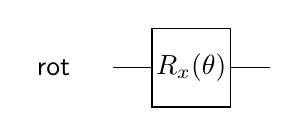
\begin{tikzpicture}[scale=.5] \node[draw=none] at (-3.5, 0) {rot}; \draw (-2,0) -- (-1, 0); \draw (1, 0) -- (2, 0); \draw (-1,-1)--(-1,1)--(1,1)--(1,-1)--cycle; \node[draw=none] at (0, 0) {$R_x(\theta)$}; \end{tikzpicture} } \]


\begin{DoxyParams}[1]{Parameters}
\mbox{\tt in,out}  & {\em multi\+Qubit} & object representing the set of all qubits \\
\hline
\mbox{\tt in}  & {\em rot\+Qubit} & qubit to rotate \\
\hline
\mbox{\tt in}  & {\em angle} & angle by which to rotate in radians \\
\hline
\end{DoxyParams}

\begin{DoxyExceptions}{Exceptions}
{\em exit\+With\+Error} & if {\ttfamily rot\+Qubit} is outside \mbox{[}0, {\ttfamily multi\+Qubit.\+num\+Qubits}). \\
\hline
\end{DoxyExceptions}


Definition at line 120 of file Qu\+E\+S\+T.\+cpp.



References rotate\+Around\+Axis().


\begin{DoxyCode}
120                                                                    \{
121 
122     \mbox{\hyperlink{structVector}{Vector}} unitAxis = \{1, 0, 0\};
123     \mbox{\hyperlink{QuEST_8cpp_a8810423457803005fecd415f4299f40d}{rotateAroundAxis}}(multiQubit, rotQubit, angle, unitAxis);
124 \}
\end{DoxyCode}
\mbox{\Hypertarget{QuEST_8cpp_ace0d3592d38a990e81a434c4e9681500}\label{QuEST_8cpp_ace0d3592d38a990e81a434c4e9681500}} 
\index{Qu\+E\+S\+T.\+cpp@{Qu\+E\+S\+T.\+cpp}!rotateY@{rotateY}}
\index{rotateY@{rotateY}!Qu\+E\+S\+T.\+cpp@{Qu\+E\+S\+T.\+cpp}}
\paragraph{\texorpdfstring{rotate\+Y()}{rotateY()}}
{\footnotesize\ttfamily void rotateY (\begin{DoxyParamCaption}\item[{\mbox{\hyperlink{structMultiQubit}{Multi\+Qubit}}}]{multi\+Qubit,  }\item[{const int}]{rot\+Qubit,  }\item[{\mbox{\hyperlink{QuEST__precision_8h_a4b654506f18b8bfd61ad2a29a7e38c25}{R\+E\+AL}}}]{angle }\end{DoxyParamCaption})}



Rotate a single qubit by a given angle around the Y-\/axis of the Bloch-\/sphere. 

For angle $\theta$, applies \[ \begin{pmatrix} \cos\theta/2 & \sin \theta/2\\ \sin \theta/2 & \cos \theta/2 \end{pmatrix} \] ~\newline
 \[ \setlength{\fboxrule}{0.01pt} \fbox{ 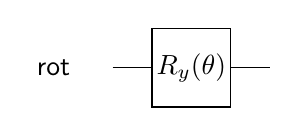
\begin{tikzpicture}[scale=.5] \node[draw=none] at (-3.5, 0) {rot}; \draw (-2,0) -- (-1, 0); \draw (1, 0) -- (2, 0); \draw (-1,-1)--(-1,1)--(1,1)--(1,-1)--cycle; \node[draw=none] at (0, 0) {$R_y(\theta)$}; \end{tikzpicture} } \]


\begin{DoxyParams}[1]{Parameters}
\mbox{\tt in,out}  & {\em multi\+Qubit} & object representing the set of all qubits \\
\hline
\mbox{\tt in}  & {\em rot\+Qubit} & qubit to rotate \\
\hline
\mbox{\tt in}  & {\em angle} & angle by which to rotate in radians \\
\hline
\end{DoxyParams}

\begin{DoxyExceptions}{Exceptions}
{\em exit\+With\+Error} & if {\ttfamily rot\+Qubit} is outside \mbox{[}0, {\ttfamily multi\+Qubit.\+num\+Qubits}). \\
\hline
\end{DoxyExceptions}


Definition at line 126 of file Qu\+E\+S\+T.\+cpp.



References rotate\+Around\+Axis().


\begin{DoxyCode}
126                                                                    \{
127 
128     \mbox{\hyperlink{structVector}{Vector}} unitAxis = \{0, 1, 0\};
129     \mbox{\hyperlink{QuEST_8cpp_a8810423457803005fecd415f4299f40d}{rotateAroundAxis}}(multiQubit, rotQubit, angle, unitAxis);
130 \}
\end{DoxyCode}
\mbox{\Hypertarget{QuEST_8cpp_abd621412ad30c1b034f4ce153c4afe10}\label{QuEST_8cpp_abd621412ad30c1b034f4ce153c4afe10}} 
\index{Qu\+E\+S\+T.\+cpp@{Qu\+E\+S\+T.\+cpp}!rotateZ@{rotateZ}}
\index{rotateZ@{rotateZ}!Qu\+E\+S\+T.\+cpp@{Qu\+E\+S\+T.\+cpp}}
\paragraph{\texorpdfstring{rotate\+Z()}{rotateZ()}}
{\footnotesize\ttfamily void rotateZ (\begin{DoxyParamCaption}\item[{\mbox{\hyperlink{structMultiQubit}{Multi\+Qubit}}}]{multi\+Qubit,  }\item[{const int}]{rot\+Qubit,  }\item[{\mbox{\hyperlink{QuEST__precision_8h_a4b654506f18b8bfd61ad2a29a7e38c25}{R\+E\+AL}}}]{angle }\end{DoxyParamCaption})}



Rotate a single qubit by a given angle around the Z-\/axis of the Bloch-\/sphere (also known as a phase shift gate). 

For angle $\theta$, applies \[ \begin{pmatrix} \exp(-i \theta/2) & 0 \\ 0 & \exp(i \theta/2) \end{pmatrix} \]

\[ \setlength{\fboxrule}{0.01pt} \fbox{ 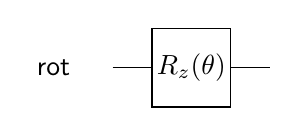
\begin{tikzpicture}[scale=.5] \node[draw=none] at (-3.5, 0) {rot}; \draw (-2,0) -- (-1, 0); \draw (1, 0) -- (2, 0); \draw (-1,-1)--(-1,1)--(1,1)--(1,-1)--cycle; \node[draw=none] at (0, 0) {$R_z(\theta)$}; \end{tikzpicture} } \]


\begin{DoxyParams}[1]{Parameters}
\mbox{\tt in,out}  & {\em multi\+Qubit} & object representing the set of all qubits \\
\hline
\mbox{\tt in}  & {\em rot\+Qubit} & qubit to rotate \\
\hline
\mbox{\tt in}  & {\em angle} & angle by which to rotate in radians \\
\hline
\end{DoxyParams}

\begin{DoxyExceptions}{Exceptions}
{\em exit\+With\+Error} & if {\ttfamily rot\+Qubit} is outside \mbox{[}0, {\ttfamily multi\+Qubit.\+num\+Qubits}). \\
\hline
\end{DoxyExceptions}


Definition at line 132 of file Qu\+E\+S\+T.\+cpp.



References rotate\+Around\+Axis().


\begin{DoxyCode}
132                                                                    \{
133 
134     \mbox{\hyperlink{structVector}{Vector}} unitAxis = \{0, 0, 1\};
135     \mbox{\hyperlink{QuEST_8cpp_a8810423457803005fecd415f4299f40d}{rotateAroundAxis}}(multiQubit, rotQubit, angle, unitAxis);
136 \}
\end{DoxyCode}
\mbox{\Hypertarget{QuEST_8cpp_adda6c47876a7676488ed0565a19eaa65}\label{QuEST_8cpp_adda6c47876a7676488ed0565a19eaa65}} 
\index{Qu\+E\+S\+T.\+cpp@{Qu\+E\+S\+T.\+cpp}!s\+Gate@{s\+Gate}}
\index{s\+Gate@{s\+Gate}!Qu\+E\+S\+T.\+cpp@{Qu\+E\+S\+T.\+cpp}}
\paragraph{\texorpdfstring{s\+Gate()}{sGate()}}
{\footnotesize\ttfamily void s\+Gate (\begin{DoxyParamCaption}\item[{\mbox{\hyperlink{structMultiQubit}{Multi\+Qubit}}}]{multi\+Qubit,  }\item[{const int}]{target\+Qubit }\end{DoxyParamCaption})}



Apply the single-\/qubit S gate. 

This is a rotation of $\pi/2$ around the Z-\/axis on the Bloch sphere, or the unitary\+: \[ \begin{pmatrix} 1 & 0 \\ 0 & i \end{pmatrix} \]

\[ \setlength{\fboxrule}{0.01pt} \fbox{ 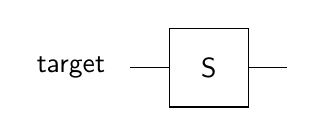
\begin{tikzpicture}[scale=.5] \node[draw=none] at (-3.5, 0) {target}; \draw (-2,0) -- (-1, 0); \draw (1, 0) -- (2, 0); \draw (-1,-1)--(-1,1)--(1,1)--(1,-1)--cycle; \node[draw=none] at (0, 0) {S}; \end{tikzpicture} } \]


\begin{DoxyParams}[1]{Parameters}
\mbox{\tt in,out}  & {\em multi\+Qubit} & object representing the set of all qubits \\
\hline
\mbox{\tt in}  & {\em target\+Qubit} & qubit to operate upon \\
\hline
\end{DoxyParams}

\begin{DoxyExceptions}{Exceptions}
{\em exit\+With\+Error} & if {\ttfamily target\+Qubit} is outside \mbox{[}0, {\ttfamily multi\+Qubit.\+num\+Qubits}) \\
\hline
\end{DoxyExceptions}


Definition at line 174 of file Qu\+E\+S\+T.\+cpp.



References phase\+Gate(), and S\+\_\+\+G\+A\+TE.


\begin{DoxyCode}
175 \{
176     \mbox{\hyperlink{QuEST__internal_8h_aae7a8a7f1ccbddb7f76b6c52b746bb43}{phaseGate}}(multiQubit, targetQubit, \mbox{\hyperlink{QuEST_8h_a5739021c733cecc49647956b2f7338eaa06e60f80fa80cce271793d6d31bcc21f}{S\_GATE}});
177 \} 
\end{DoxyCode}
\mbox{\Hypertarget{QuEST_8cpp_aebaab86326779de55d335cfea3efde8f}\label{QuEST_8cpp_aebaab86326779de55d335cfea3efde8f}} 
\index{Qu\+E\+S\+T.\+cpp@{Qu\+E\+S\+T.\+cpp}!sigmaZ@{sigmaZ}}
\index{sigmaZ@{sigmaZ}!Qu\+E\+S\+T.\+cpp@{Qu\+E\+S\+T.\+cpp}}
\paragraph{\texorpdfstring{sigma\+Z()}{sigmaZ()}}
{\footnotesize\ttfamily void sigmaZ (\begin{DoxyParamCaption}\item[{\mbox{\hyperlink{structMultiQubit}{Multi\+Qubit}}}]{multi\+Qubit,  }\item[{const int}]{target\+Qubit }\end{DoxyParamCaption})}



Apply the single-\/qubit sigma-\/Z (also known as the Z, Pauli-\/Z or phase-\/flip) gate. 

This is a rotation of $\pi$ around the Z-\/axis (a phase shift) on the Bloch sphere. I.\+e. \[ \begin{pmatrix} 1 & 0 \\ 0 & -1 \end{pmatrix} \] ~\newline
 \[ \setlength{\fboxrule}{0.01pt} \fbox{ 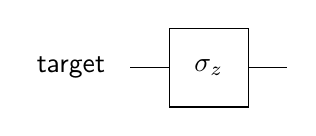
\begin{tikzpicture}[scale=.5] \node[draw=none] at (-3.5, 0) {target}; \draw (-2,0) -- (-1, 0); \draw (1, 0) -- (2, 0); \draw (-1,-1)--(-1,1)--(1,1)--(1,-1)--cycle; \node[draw=none] at (0, 0) {$\sigma_z$}; \end{tikzpicture} } \] ~\newline
 
\begin{DoxyParams}[1]{Parameters}
\mbox{\tt in,out}  & {\em multi\+Qubit} & object representing the set of all qubits \\
\hline
\mbox{\tt in}  & {\em target\+Qubit} & qubit to operate on \\
\hline
\end{DoxyParams}

\begin{DoxyExceptions}{Exceptions}
{\em exit\+With\+Error} & if {\ttfamily target\+Qubit} is outside \mbox{[}0, {\ttfamily multi\+Qubit.\+num\+Qubits}). \\
\hline
\end{DoxyExceptions}


Definition at line 169 of file Qu\+E\+S\+T.\+cpp.



References phase\+Gate(), and S\+I\+G\+M\+A\+\_\+Z.


\begin{DoxyCode}
170 \{
171     \mbox{\hyperlink{QuEST__internal_8h_aae7a8a7f1ccbddb7f76b6c52b746bb43}{phaseGate}}(multiQubit, targetQubit, \mbox{\hyperlink{QuEST_8h_a5739021c733cecc49647956b2f7338eaa754922d1e1846a1961ff2bf163483dac}{SIGMA\_Z}});
172 \}
\end{DoxyCode}
\mbox{\Hypertarget{QuEST_8cpp_af764ea63a2e870098f4e1ce08562942e}\label{QuEST_8cpp_af764ea63a2e870098f4e1ce08562942e}} 
\index{Qu\+E\+S\+T.\+cpp@{Qu\+E\+S\+T.\+cpp}!t\+Gate@{t\+Gate}}
\index{t\+Gate@{t\+Gate}!Qu\+E\+S\+T.\+cpp@{Qu\+E\+S\+T.\+cpp}}
\paragraph{\texorpdfstring{t\+Gate()}{tGate()}}
{\footnotesize\ttfamily void t\+Gate (\begin{DoxyParamCaption}\item[{\mbox{\hyperlink{structMultiQubit}{Multi\+Qubit}}}]{multi\+Qubit,  }\item[{const int}]{target\+Qubit }\end{DoxyParamCaption})}



Apply the single-\/qubit T gate. 

This is a rotation of $\pi/4$ around the Z-\/axis on the Bloch sphere, or the unitary\+: \[ \begin{pmatrix} 1 & 0 \\ 0 & \exp\left(i \frac{\pi}{4}\right) \end{pmatrix} \]

\[ \setlength{\fboxrule}{0.01pt} \fbox{ 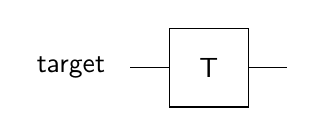
\begin{tikzpicture}[scale=.5] \node[draw=none] at (-3.5, 0) {target}; \draw (-2,0) -- (-1, 0); \draw (1, 0) -- (2, 0); \draw (-1,-1)--(-1,1)--(1,1)--(1,-1)--cycle; \node[draw=none] at (0, 0) {T}; \end{tikzpicture} } \]


\begin{DoxyParams}[1]{Parameters}
\mbox{\tt in,out}  & {\em multi\+Qubit} & object representing the set of all qubits \\
\hline
\mbox{\tt in}  & {\em target\+Qubit} & qubit to operate upon \\
\hline
\end{DoxyParams}

\begin{DoxyExceptions}{Exceptions}
{\em exit\+With\+Error} & if {\ttfamily target\+Qubit} is outside \mbox{[}0, {\ttfamily multi\+Qubit.\+num\+Qubits}) \\
\hline
\end{DoxyExceptions}


Definition at line 179 of file Qu\+E\+S\+T.\+cpp.



References phase\+Gate(), and T\+\_\+\+G\+A\+TE.


\begin{DoxyCode}
180 \{
181     \mbox{\hyperlink{QuEST__internal_8h_aae7a8a7f1ccbddb7f76b6c52b746bb43}{phaseGate}}(multiQubit, targetQubit, \mbox{\hyperlink{QuEST_8h_a5739021c733cecc49647956b2f7338eaa614d07d597a8e320cc556bc0e652e4ab}{T\_GATE}});
182 \}
\end{DoxyCode}
\mbox{\Hypertarget{QuEST_8cpp_ae2b2c14a07dd7d50ff86032a3ca101d7}\label{QuEST_8cpp_ae2b2c14a07dd7d50ff86032a3ca101d7}} 
\index{Qu\+E\+S\+T.\+cpp@{Qu\+E\+S\+T.\+cpp}!validate\+Alpha\+Beta@{validate\+Alpha\+Beta}}
\index{validate\+Alpha\+Beta@{validate\+Alpha\+Beta}!Qu\+E\+S\+T.\+cpp@{Qu\+E\+S\+T.\+cpp}}
\paragraph{\texorpdfstring{validate\+Alpha\+Beta()}{validateAlphaBeta()}}
{\footnotesize\ttfamily int validate\+Alpha\+Beta (\begin{DoxyParamCaption}\item[{\mbox{\hyperlink{structComplex}{Complex}}}]{alpha,  }\item[{\mbox{\hyperlink{structComplex}{Complex}}}]{beta }\end{DoxyParamCaption})}



Definition at line 209 of file Qu\+E\+S\+T.\+cpp.



References Complex\+::imag, Complex\+::real, and R\+E\+A\+L\+\_\+\+E\+PS.


\begin{DoxyCode}
209                                                   \{
210     \textcolor{keywordflow}{if} ( fabs(alpha.\mbox{\hyperlink{structComplex_a479ad939835457595fcca3ca55c06283}{real}}*alpha.\mbox{\hyperlink{structComplex_a479ad939835457595fcca3ca55c06283}{real}} 
211         + alpha.\mbox{\hyperlink{structComplex_a1151948284b21c0052f203f23ab931d9}{imag}}*alpha.\mbox{\hyperlink{structComplex_a1151948284b21c0052f203f23ab931d9}{imag}}
212         + beta.\mbox{\hyperlink{structComplex_a479ad939835457595fcca3ca55c06283}{real}}*beta.\mbox{\hyperlink{structComplex_a479ad939835457595fcca3ca55c06283}{real}} 
213         + beta.\mbox{\hyperlink{structComplex_a1151948284b21c0052f203f23ab931d9}{imag}}*beta.\mbox{\hyperlink{structComplex_a1151948284b21c0052f203f23ab931d9}{imag}} - 1) > \mbox{\hyperlink{QuEST__precision_8h_aebb5e6716e06431296af4d1a71744dec}{REAL\_EPS}} ) \textcolor{keywordflow}{return} 0;
214     \textcolor{keywordflow}{else} \textcolor{keywordflow}{return} 1;
215 \}
\end{DoxyCode}
\mbox{\Hypertarget{QuEST_8cpp_ae4fea133d1a8f09ff8da03038100adb2}\label{QuEST_8cpp_ae4fea133d1a8f09ff8da03038100adb2}} 
\index{Qu\+E\+S\+T.\+cpp@{Qu\+E\+S\+T.\+cpp}!validate\+Matrix\+Is\+Unitary@{validate\+Matrix\+Is\+Unitary}}
\index{validate\+Matrix\+Is\+Unitary@{validate\+Matrix\+Is\+Unitary}!Qu\+E\+S\+T.\+cpp@{Qu\+E\+S\+T.\+cpp}}
\paragraph{\texorpdfstring{validate\+Matrix\+Is\+Unitary()}{validateMatrixIsUnitary()}}
{\footnotesize\ttfamily int validate\+Matrix\+Is\+Unitary (\begin{DoxyParamCaption}\item[{\mbox{\hyperlink{structComplexMatrix2}{Complex\+Matrix2}}}]{u }\end{DoxyParamCaption})}



Definition at line 184 of file Qu\+E\+S\+T.\+cpp.



References Complex\+::imag, Complex\+Matrix2\+::r0c0, Complex\+Matrix2\+::r0c1, Complex\+Matrix2\+::r1c0, Complex\+Matrix2\+::r1c1, Complex\+::real, and R\+E\+A\+L\+\_\+\+E\+PS.


\begin{DoxyCode}
184                                              \{
185 
186     \textcolor{keywordflow}{if} ( fabs(u.\mbox{\hyperlink{structComplexMatrix2_ae72b4458233b077a636beee1892e81ff}{r0c0}}.\mbox{\hyperlink{structComplex_a479ad939835457595fcca3ca55c06283}{real}}*u.\mbox{\hyperlink{structComplexMatrix2_ae72b4458233b077a636beee1892e81ff}{r0c0}}.\mbox{\hyperlink{structComplex_a479ad939835457595fcca3ca55c06283}{real}} 
187         + u.\mbox{\hyperlink{structComplexMatrix2_ae72b4458233b077a636beee1892e81ff}{r0c0}}.\mbox{\hyperlink{structComplex_a1151948284b21c0052f203f23ab931d9}{imag}}*u.\mbox{\hyperlink{structComplexMatrix2_ae72b4458233b077a636beee1892e81ff}{r0c0}}.\mbox{\hyperlink{structComplex_a1151948284b21c0052f203f23ab931d9}{imag}}
188         + u.\mbox{\hyperlink{structComplexMatrix2_ab98282015ed2065e53fbc9638e2583ab}{r1c0}}.\mbox{\hyperlink{structComplex_a479ad939835457595fcca3ca55c06283}{real}}*u.\mbox{\hyperlink{structComplexMatrix2_ab98282015ed2065e53fbc9638e2583ab}{r1c0}}.\mbox{\hyperlink{structComplex_a479ad939835457595fcca3ca55c06283}{real}}
189         + u.\mbox{\hyperlink{structComplexMatrix2_ab98282015ed2065e53fbc9638e2583ab}{r1c0}}.\mbox{\hyperlink{structComplex_a1151948284b21c0052f203f23ab931d9}{imag}}*u.\mbox{\hyperlink{structComplexMatrix2_ab98282015ed2065e53fbc9638e2583ab}{r1c0}}.\mbox{\hyperlink{structComplex_a1151948284b21c0052f203f23ab931d9}{imag}} - 1) > \mbox{\hyperlink{QuEST__precision_8h_aebb5e6716e06431296af4d1a71744dec}{REAL\_EPS}} ) \textcolor{keywordflow}{return} 0;
190     \textcolor{comment}{// check}
191     \textcolor{keywordflow}{if} ( fabs(u.\mbox{\hyperlink{structComplexMatrix2_a0f3932f055a8b05cef361bce25d51172}{r0c1}}.\mbox{\hyperlink{structComplex_a479ad939835457595fcca3ca55c06283}{real}}*u.\mbox{\hyperlink{structComplexMatrix2_a0f3932f055a8b05cef361bce25d51172}{r0c1}}.\mbox{\hyperlink{structComplex_a479ad939835457595fcca3ca55c06283}{real}} 
192         + u.\mbox{\hyperlink{structComplexMatrix2_a0f3932f055a8b05cef361bce25d51172}{r0c1}}.\mbox{\hyperlink{structComplex_a1151948284b21c0052f203f23ab931d9}{imag}}*u.\mbox{\hyperlink{structComplexMatrix2_a0f3932f055a8b05cef361bce25d51172}{r0c1}}.\mbox{\hyperlink{structComplex_a1151948284b21c0052f203f23ab931d9}{imag}}
193         + u.\mbox{\hyperlink{structComplexMatrix2_a763007c3070802373549ba0350f83c8a}{r1c1}}.\mbox{\hyperlink{structComplex_a479ad939835457595fcca3ca55c06283}{real}}*u.\mbox{\hyperlink{structComplexMatrix2_a763007c3070802373549ba0350f83c8a}{r1c1}}.\mbox{\hyperlink{structComplex_a479ad939835457595fcca3ca55c06283}{real}}
194         + u.\mbox{\hyperlink{structComplexMatrix2_a763007c3070802373549ba0350f83c8a}{r1c1}}.\mbox{\hyperlink{structComplex_a1151948284b21c0052f203f23ab931d9}{imag}}*u.\mbox{\hyperlink{structComplexMatrix2_a763007c3070802373549ba0350f83c8a}{r1c1}}.\mbox{\hyperlink{structComplex_a1151948284b21c0052f203f23ab931d9}{imag}} - 1) > \mbox{\hyperlink{QuEST__precision_8h_aebb5e6716e06431296af4d1a71744dec}{REAL\_EPS}} ) \textcolor{keywordflow}{return} 0;
195 
196     \textcolor{keywordflow}{if} ( fabs(u.\mbox{\hyperlink{structComplexMatrix2_ae72b4458233b077a636beee1892e81ff}{r0c0}}.\mbox{\hyperlink{structComplex_a479ad939835457595fcca3ca55c06283}{real}}*u.\mbox{\hyperlink{structComplexMatrix2_a0f3932f055a8b05cef361bce25d51172}{r0c1}}.\mbox{\hyperlink{structComplex_a479ad939835457595fcca3ca55c06283}{real}} 
197         + u.\mbox{\hyperlink{structComplexMatrix2_ae72b4458233b077a636beee1892e81ff}{r0c0}}.\mbox{\hyperlink{structComplex_a1151948284b21c0052f203f23ab931d9}{imag}}*u.\mbox{\hyperlink{structComplexMatrix2_a0f3932f055a8b05cef361bce25d51172}{r0c1}}.\mbox{\hyperlink{structComplex_a1151948284b21c0052f203f23ab931d9}{imag}}
198         + u.\mbox{\hyperlink{structComplexMatrix2_ab98282015ed2065e53fbc9638e2583ab}{r1c0}}.\mbox{\hyperlink{structComplex_a479ad939835457595fcca3ca55c06283}{real}}*u.\mbox{\hyperlink{structComplexMatrix2_a763007c3070802373549ba0350f83c8a}{r1c1}}.\mbox{\hyperlink{structComplex_a479ad939835457595fcca3ca55c06283}{real}}
199         + u.\mbox{\hyperlink{structComplexMatrix2_ab98282015ed2065e53fbc9638e2583ab}{r1c0}}.\mbox{\hyperlink{structComplex_a1151948284b21c0052f203f23ab931d9}{imag}}*u.\mbox{\hyperlink{structComplexMatrix2_a763007c3070802373549ba0350f83c8a}{r1c1}}.\mbox{\hyperlink{structComplex_a1151948284b21c0052f203f23ab931d9}{imag}}) > \mbox{\hyperlink{QuEST__precision_8h_aebb5e6716e06431296af4d1a71744dec}{REAL\_EPS}} ) \textcolor{keywordflow}{return} 0;
200 
201     \textcolor{keywordflow}{if} ( fabs(u.\mbox{\hyperlink{structComplexMatrix2_a0f3932f055a8b05cef361bce25d51172}{r0c1}}.\mbox{\hyperlink{structComplex_a479ad939835457595fcca3ca55c06283}{real}}*u.\mbox{\hyperlink{structComplexMatrix2_ae72b4458233b077a636beee1892e81ff}{r0c0}}.\mbox{\hyperlink{structComplex_a1151948284b21c0052f203f23ab931d9}{imag}}
202         - u.\mbox{\hyperlink{structComplexMatrix2_ae72b4458233b077a636beee1892e81ff}{r0c0}}.\mbox{\hyperlink{structComplex_a479ad939835457595fcca3ca55c06283}{real}}*u.\mbox{\hyperlink{structComplexMatrix2_a0f3932f055a8b05cef361bce25d51172}{r0c1}}.\mbox{\hyperlink{structComplex_a1151948284b21c0052f203f23ab931d9}{imag}}
203         + u.\mbox{\hyperlink{structComplexMatrix2_a763007c3070802373549ba0350f83c8a}{r1c1}}.\mbox{\hyperlink{structComplex_a479ad939835457595fcca3ca55c06283}{real}}*u.\mbox{\hyperlink{structComplexMatrix2_ab98282015ed2065e53fbc9638e2583ab}{r1c0}}.\mbox{\hyperlink{structComplex_a1151948284b21c0052f203f23ab931d9}{imag}}
204         - u.\mbox{\hyperlink{structComplexMatrix2_ab98282015ed2065e53fbc9638e2583ab}{r1c0}}.\mbox{\hyperlink{structComplex_a479ad939835457595fcca3ca55c06283}{real}}*u.\mbox{\hyperlink{structComplexMatrix2_a763007c3070802373549ba0350f83c8a}{r1c1}}.\mbox{\hyperlink{structComplex_a1151948284b21c0052f203f23ab931d9}{imag}}) > \mbox{\hyperlink{QuEST__precision_8h_aebb5e6716e06431296af4d1a71744dec}{REAL\_EPS}} ) \textcolor{keywordflow}{return} 0;
205 
206     \textcolor{keywordflow}{return} 1;
207 \}
\end{DoxyCode}
\mbox{\Hypertarget{QuEST_8cpp_a71c14976f63cfcda70026fa20ee531fe}\label{QuEST_8cpp_a71c14976f63cfcda70026fa20ee531fe}} 
\index{Qu\+E\+S\+T.\+cpp@{Qu\+E\+S\+T.\+cpp}!validate\+Unit\+Vector@{validate\+Unit\+Vector}}
\index{validate\+Unit\+Vector@{validate\+Unit\+Vector}!Qu\+E\+S\+T.\+cpp@{Qu\+E\+S\+T.\+cpp}}
\paragraph{\texorpdfstring{validate\+Unit\+Vector()}{validateUnitVector()}}
{\footnotesize\ttfamily int validate\+Unit\+Vector (\begin{DoxyParamCaption}\item[{\mbox{\hyperlink{QuEST__precision_8h_a4b654506f18b8bfd61ad2a29a7e38c25}{R\+E\+AL}}}]{ux,  }\item[{\mbox{\hyperlink{QuEST__precision_8h_a4b654506f18b8bfd61ad2a29a7e38c25}{R\+E\+AL}}}]{uy,  }\item[{\mbox{\hyperlink{QuEST__precision_8h_a4b654506f18b8bfd61ad2a29a7e38c25}{R\+E\+AL}}}]{uz }\end{DoxyParamCaption})}



Definition at line 217 of file Qu\+E\+S\+T.\+cpp.



References R\+E\+A\+L\+\_\+\+E\+PS.


\begin{DoxyCode}
217                                                  \{
218     \textcolor{keywordflow}{if} ( fabs(sqrt(ux*ux + uy*uy + uz*uz) - 1) > \mbox{\hyperlink{QuEST__precision_8h_aebb5e6716e06431296af4d1a71744dec}{REAL\_EPS}} ) \textcolor{keywordflow}{return} 0;
219     \textcolor{keywordflow}{else} \textcolor{keywordflow}{return} 1;
220 \}
\end{DoxyCode}


\subsubsection{Variable Documentation}
\mbox{\Hypertarget{QuEST_8cpp_aac1637696885c75b73a1ecf381cea713}\label{QuEST_8cpp_aac1637696885c75b73a1ecf381cea713}} 
\index{Qu\+E\+S\+T.\+cpp@{Qu\+E\+S\+T.\+cpp}!error\+Codes@{error\+Codes}}
\index{error\+Codes@{error\+Codes}!Qu\+E\+S\+T.\+cpp@{Qu\+E\+S\+T.\+cpp}}
\paragraph{\texorpdfstring{error\+Codes}{errorCodes}}
{\footnotesize\ttfamily const char$\ast$ error\+Codes\mbox{[}$\,$\mbox{]}}

{\bfseries Initial value\+:}
\begin{DoxyCode}
= \{
    \textcolor{stringliteral}{"Success"},                                              
    \textcolor{stringliteral}{"Invalid target qubit. Note qubits are zero indexed."},  
    \textcolor{stringliteral}{"Invalid control qubit. Note qubits are zero indexed."}, 
    \textcolor{stringliteral}{"Control qubit cannot equal target qubit."},             
    \textcolor{stringliteral}{"Invalid number of control qubits"},                     
    \textcolor{stringliteral}{"Invalid unitary matrix."},                              
    \textcolor{stringliteral}{"Invalid rotation arguments."},                          
    \textcolor{stringliteral}{"Invalid system size. Cannot print output for systems greater than 5 qubits."}, 
    \textcolor{stringliteral}{"Can't collapse to state with zero probability."}, 
    \textcolor{stringliteral}{"Invalid number of qubits."}, 
    \textcolor{stringliteral}{"Invalid measurement outcome -- must be either 0 or 1."} 
\}
\end{DoxyCode}


Definition at line 24 of file Qu\+E\+S\+T.\+cpp.


\hypertarget{QuEST_8h}{}\subsection{Qu\+E\+S\+T.\+h File Reference}
\label{QuEST_8h}\index{Qu\+E\+S\+T.\+h@{Qu\+E\+S\+T.\+h}}


The Qu\+E\+ST library A\+PI and objects.  


{\ttfamily \#include \char`\"{}Qu\+E\+S\+T\+\_\+precision.\+h\char`\"{}}\newline
\subsubsection*{Data Structures}
\begin{DoxyCompactItemize}
\item 
struct \mbox{\hyperlink{structComplex}{Complex}}
\begin{DoxyCompactList}\small\item\em Represents one complex number. \end{DoxyCompactList}\item 
struct \mbox{\hyperlink{structComplexArray}{Complex\+Array}}
\begin{DoxyCompactList}\small\item\em Represents an array of complex numbers grouped into an array of real components and an array of coressponding complex components. \end{DoxyCompactList}\item 
struct \mbox{\hyperlink{structComplexMatrix2}{Complex\+Matrix2}}
\begin{DoxyCompactList}\small\item\em Represents a 2x2 matrix of complex numbers. \end{DoxyCompactList}\item 
struct \mbox{\hyperlink{structMultiQubit}{Multi\+Qubit}}
\begin{DoxyCompactList}\small\item\em Represents a system of qubits. \end{DoxyCompactList}\item 
struct \mbox{\hyperlink{structQuESTEnv}{Qu\+E\+S\+T\+Env}}
\begin{DoxyCompactList}\small\item\em Information about the environment the program is running in. \end{DoxyCompactList}\item 
struct \mbox{\hyperlink{structVector}{Vector}}
\begin{DoxyCompactList}\small\item\em Represents a 3-\/vector of real numbers. \end{DoxyCompactList}\end{DoxyCompactItemize}
\subsubsection*{Typedefs}
\begin{DoxyCompactItemize}
\item 
typedef struct \mbox{\hyperlink{structComplex}{Complex}} \mbox{\hyperlink{QuEST_8h_ad59c9e471673c07782e6c403277ffd8d}{Complex}}
\begin{DoxyCompactList}\small\item\em Represents one complex number. \end{DoxyCompactList}\item 
typedef struct \mbox{\hyperlink{structComplexArray}{Complex\+Array}} \mbox{\hyperlink{QuEST_8h_a19e00739fde70a851d068f322cf915c8}{Complex\+Array}}
\begin{DoxyCompactList}\small\item\em Represents an array of complex numbers grouped into an array of real components and an array of coressponding complex components. \end{DoxyCompactList}\item 
typedef struct \mbox{\hyperlink{structComplexMatrix2}{Complex\+Matrix2}} \mbox{\hyperlink{QuEST_8h_aa6e00518bd2c71030c52d5955e506875}{Complex\+Matrix2}}
\begin{DoxyCompactList}\small\item\em Represents a 2x2 matrix of complex numbers. \end{DoxyCompactList}\item 
typedef struct \mbox{\hyperlink{structMultiQubit}{Multi\+Qubit}} \mbox{\hyperlink{QuEST_8h_af4123a681074068eeeee1562758eef61}{Multi\+Qubit}}
\begin{DoxyCompactList}\small\item\em Represents a system of qubits. \end{DoxyCompactList}\item 
typedef struct \mbox{\hyperlink{structQuESTEnv}{Qu\+E\+S\+T\+Env}} \mbox{\hyperlink{QuEST_8h_aedfe2bb713c31d6133e53b1bd72d7a2c}{Qu\+E\+S\+T\+Env}}
\begin{DoxyCompactList}\small\item\em Information about the environment the program is running in. \end{DoxyCompactList}\item 
typedef struct \mbox{\hyperlink{structVector}{Vector}} \mbox{\hyperlink{QuEST_8h_a6ded2cf071c127e518317e3c451af3ef}{Vector}}
\begin{DoxyCompactList}\small\item\em Represents a 3-\/vector of real numbers. \end{DoxyCompactList}\end{DoxyCompactItemize}
\subsubsection*{Enumerations}
\begin{DoxyCompactItemize}
\item 
enum \mbox{\hyperlink{QuEST_8h_a5739021c733cecc49647956b2f7338ea}{phase\+Gate\+Type}} \{ \mbox{\hyperlink{QuEST_8h_a5739021c733cecc49647956b2f7338eaa754922d1e1846a1961ff2bf163483dac}{S\+I\+G\+M\+A\+\_\+Z}} =0, 
\mbox{\hyperlink{QuEST_8h_a5739021c733cecc49647956b2f7338eaa06e60f80fa80cce271793d6d31bcc21f}{S\+\_\+\+G\+A\+TE}} =1, 
\mbox{\hyperlink{QuEST_8h_a5739021c733cecc49647956b2f7338eaa614d07d597a8e320cc556bc0e652e4ab}{T\+\_\+\+G\+A\+TE}} =2
 \}
\end{DoxyCompactItemize}
\subsubsection*{Functions}
\begin{DoxyCompactItemize}
\item 
\mbox{\hyperlink{QuEST__precision_8h_a4b654506f18b8bfd61ad2a29a7e38c25}{R\+E\+AL}} \mbox{\hyperlink{QuEST_8h_a818a4c7cd7252d2b10b896b12fa431d3}{calc\+Total\+Probability}} (\mbox{\hyperlink{structMultiQubit}{Multi\+Qubit}} multi\+Qubit)
\begin{DoxyCompactList}\small\item\em Calculate the probability of being in any state by taking the norm of the entire state vector. \end{DoxyCompactList}\item 
void \mbox{\hyperlink{QuEST_8h_abd4bc926cd3f9b65610bb228d0c59fe0}{close\+Qu\+E\+S\+T\+Env}} (\mbox{\hyperlink{structQuESTEnv}{Qu\+E\+S\+T\+Env}} \mbox{\hyperlink{runTests_8c_a5fd8ba97fcae3408ae6221dfc3cc1f93}{env}})
\begin{DoxyCompactList}\small\item\em Close Qu\+E\+ST environment. \end{DoxyCompactList}\item 
\mbox{\hyperlink{QuEST__precision_8h_a4b654506f18b8bfd61ad2a29a7e38c25}{R\+E\+AL}} \mbox{\hyperlink{QuEST_8h_a07418ebac70fd9ae5d051d089961631d}{collapse\+To\+Outcome}} (\mbox{\hyperlink{structMultiQubit}{Multi\+Qubit}} multi\+Qubit, const int measure\+Qubit, int outcome)
\begin{DoxyCompactList}\small\item\em Updates the state vector to be consistent with measuring the measure qubit in the given outcome (0 or 1), and returns the probability of such a measurement outcome. \end{DoxyCompactList}\item 
void \mbox{\hyperlink{QuEST_8h_a03b13dfcabd8c59b50dbdd3af44ba8b2}{compact\+Unitary}} (\mbox{\hyperlink{structMultiQubit}{Multi\+Qubit}} multi\+Qubit, const int target\+Qubit, \mbox{\hyperlink{structComplex}{Complex}} alpha, \mbox{\hyperlink{structComplex}{Complex}} beta)
\begin{DoxyCompactList}\small\item\em Apply a single-\/qubit unitary parameterised by two given complex scalars. \end{DoxyCompactList}\item 
void \mbox{\hyperlink{QuEST_8h_ab4812953bc457405b3aa05a4c2f64f4a}{controlled\+Compact\+Unitary}} (\mbox{\hyperlink{structMultiQubit}{Multi\+Qubit}} multi\+Qubit, const int control\+Qubit, const int target\+Qubit, \mbox{\hyperlink{structComplex}{Complex}} alpha, \mbox{\hyperlink{structComplex}{Complex}} beta)
\begin{DoxyCompactList}\small\item\em Apply a controlled unitary (single control, single target) parameterised by two given complex scalars. \end{DoxyCompactList}\item 
void \mbox{\hyperlink{QuEST_8h_a67576895bbc65463481a8ea24d9b1e22}{controlled\+Not}} (\mbox{\hyperlink{structMultiQubit}{Multi\+Qubit}} multi\+Qubit, const int control\+Qubit, const int target\+Qubit)
\begin{DoxyCompactList}\small\item\em Apply the controlled not (single control, single target) gate, also known as the c-\/X, c-\/sigma-\/X, c-\/\+Pauli-\/X and c-\/bit-\/flip gate. \end{DoxyCompactList}\item 
void \mbox{\hyperlink{QuEST_8h_a11a96159191cbf1b01a1080e7f045aac}{controlled\+Phase\+Gate}} (\mbox{\hyperlink{structMultiQubit}{Multi\+Qubit}} multi\+Qubit, const int id\+Qubit1, const int id\+Qubit2)
\begin{DoxyCompactList}\small\item\em Apply the (two-\/qubit) controlled phase gate, also known as the controlled sigmaZ gate. \end{DoxyCompactList}\item 
void \mbox{\hyperlink{QuEST_8h_ad41f82b41149393a642391b67b3a287e}{controlled\+Rotate\+Around\+Axis}} (\mbox{\hyperlink{structMultiQubit}{Multi\+Qubit}} multi\+Qubit, const int control\+Qubit, const int target\+Qubit, \mbox{\hyperlink{QuEST__precision_8h_a4b654506f18b8bfd61ad2a29a7e38c25}{R\+E\+AL}} angle, \mbox{\hyperlink{structVector}{Vector}} axis)
\begin{DoxyCompactList}\small\item\em Applies a controlled rotation by a given angle around a given vector on the Bloch-\/sphere. \end{DoxyCompactList}\item 
void \mbox{\hyperlink{QuEST_8h_ac6923ac57e67d9a21096e06f6a9012f6}{controlled\+RotateX}} (\mbox{\hyperlink{structMultiQubit}{Multi\+Qubit}} multi\+Qubit, const int control\+Qubit, const int target\+Qubit, \mbox{\hyperlink{QuEST__precision_8h_a4b654506f18b8bfd61ad2a29a7e38c25}{R\+E\+AL}} angle)
\begin{DoxyCompactList}\small\item\em Applies a controlled rotation by a given angle around the X-\/axis of the Bloch-\/sphere. \end{DoxyCompactList}\item 
void \mbox{\hyperlink{QuEST_8h_a71e90a2f7292116338c062934f9d1202}{controlled\+RotateY}} (\mbox{\hyperlink{structMultiQubit}{Multi\+Qubit}} multi\+Qubit, const int control\+Qubit, const int target\+Qubit, \mbox{\hyperlink{QuEST__precision_8h_a4b654506f18b8bfd61ad2a29a7e38c25}{R\+E\+AL}} angle)
\begin{DoxyCompactList}\small\item\em Applies a controlled rotation by a given angle around the Y-\/axis of the Bloch-\/sphere. \end{DoxyCompactList}\item 
void \mbox{\hyperlink{QuEST_8h_a668e5d2634b02e98bc73675ccb11d61c}{controlled\+RotateZ}} (\mbox{\hyperlink{structMultiQubit}{Multi\+Qubit}} multi\+Qubit, const int control\+Qubit, const int target\+Qubit, \mbox{\hyperlink{QuEST__precision_8h_a4b654506f18b8bfd61ad2a29a7e38c25}{R\+E\+AL}} angle)
\begin{DoxyCompactList}\small\item\em Applies a controlled rotation by a given angle around the Z-\/axis of the Bloch-\/sphere. \end{DoxyCompactList}\item 
void \mbox{\hyperlink{QuEST_8h_a8a701526263392599aa21d0d0f05d9d8}{controlled\+Unitary}} (\mbox{\hyperlink{structMultiQubit}{Multi\+Qubit}} multi\+Qubit, const int control\+Qubit, const int target\+Qubit, \mbox{\hyperlink{structComplexMatrix2}{Complex\+Matrix2}} u)
\begin{DoxyCompactList}\small\item\em Apply a general controlled unitary (single control, single target), which can include a global phase factor. \end{DoxyCompactList}\item 
void \mbox{\hyperlink{QuEST_8h_a9c02591bc64c2918503afa231d90d83f}{create\+Multi\+Qubit}} (\mbox{\hyperlink{structMultiQubit}{Multi\+Qubit}} $\ast$multi\+Qubit, int num\+Qubits, \mbox{\hyperlink{structQuESTEnv}{Qu\+E\+S\+T\+Env}} \mbox{\hyperlink{runTests_8c_a5fd8ba97fcae3408ae6221dfc3cc1f93}{env}})
\begin{DoxyCompactList}\small\item\em Create a \mbox{\hyperlink{structMultiQubit}{Multi\+Qubit}} object representing a set of qubits. \end{DoxyCompactList}\item 
void \mbox{\hyperlink{QuEST_8h_ae5d6acc322314d7a3d8a2eccf00d3b19}{destroy\+Multi\+Qubit}} (\mbox{\hyperlink{structMultiQubit}{Multi\+Qubit}} multi\+Qubit, \mbox{\hyperlink{structQuESTEnv}{Qu\+E\+S\+T\+Env}} \mbox{\hyperlink{runTests_8c_a5fd8ba97fcae3408ae6221dfc3cc1f93}{env}})
\begin{DoxyCompactList}\small\item\em Deallocate a \mbox{\hyperlink{structMultiQubit}{Multi\+Qubit}} object representing a set of qubits. \end{DoxyCompactList}\item 
\mbox{\hyperlink{QuEST__precision_8h_a4b654506f18b8bfd61ad2a29a7e38c25}{R\+E\+AL}} \mbox{\hyperlink{QuEST_8h_ad315c941a51bc053d39ebfa2040fd32e}{find\+Probability\+Of\+Outcome}} (\mbox{\hyperlink{structMultiQubit}{Multi\+Qubit}} multi\+Qubit, const int measure\+Qubit, int outcome)
\begin{DoxyCompactList}\small\item\em Gives the probability of a specified qubit being measured in the given outcome (0 or 1). \end{DoxyCompactList}\item 
void \mbox{\hyperlink{QuEST_8h_a8f10aabf9f607f19093aee54630caa21}{get\+Environment\+String}} (\mbox{\hyperlink{structQuESTEnv}{Qu\+E\+S\+T\+Env}} \mbox{\hyperlink{runTests_8c_a5fd8ba97fcae3408ae6221dfc3cc1f93}{env}}, \mbox{\hyperlink{structMultiQubit}{Multi\+Qubit}} multi\+Qubit, char str\mbox{[}200\mbox{]})
\item 
\mbox{\hyperlink{QuEST__precision_8h_a4b654506f18b8bfd61ad2a29a7e38c25}{R\+E\+AL}} \mbox{\hyperlink{QuEST_8h_a3615f76fd5f57008d9b74bbd10533dd0}{get\+Imag\+Amp\+El}} (\mbox{\hyperlink{structMultiQubit}{Multi\+Qubit}} multi\+Qubit, long long int index)
\begin{DoxyCompactList}\small\item\em Get the imaginary component of the complex probability amplitude at an index in the state vector. \end{DoxyCompactList}\item 
int \mbox{\hyperlink{QuEST_8h_ac61ecf4fd9ab2ac8453c4eb5b0d34089}{get\+Num\+Amps}} (\mbox{\hyperlink{structMultiQubit}{Multi\+Qubit}} multi\+Qubit)
\begin{DoxyCompactList}\small\item\em Get the number of probability amplitudes in a multi\+Qubit object, given by 2$^\wedge$num\+Qubits. \end{DoxyCompactList}\item 
int \mbox{\hyperlink{QuEST_8h_a00e13dc88021b61a29fac9f3ab9ee850}{get\+Num\+Qubits}} (\mbox{\hyperlink{structMultiQubit}{Multi\+Qubit}} multi\+Qubit)
\begin{DoxyCompactList}\small\item\em Get the number of qubits in a multi\+Qubit object. \end{DoxyCompactList}\item 
\mbox{\hyperlink{QuEST__precision_8h_a4b654506f18b8bfd61ad2a29a7e38c25}{R\+E\+AL}} \mbox{\hyperlink{QuEST_8h_a799b10447d6dbdaf960a4d3eedd22014}{get\+Prob\+El}} (\mbox{\hyperlink{structMultiQubit}{Multi\+Qubit}} multi\+Qubit, long long int index)
\begin{DoxyCompactList}\small\item\em Get the probability of the state at an index in the full state vector. \end{DoxyCompactList}\item 
\mbox{\hyperlink{QuEST__precision_8h_a4b654506f18b8bfd61ad2a29a7e38c25}{R\+E\+AL}} \mbox{\hyperlink{QuEST_8h_a317b786f577fa6bc136ea7f0ee7330a7}{get\+Real\+Amp\+El}} (\mbox{\hyperlink{structMultiQubit}{Multi\+Qubit}} multi\+Qubit, long long int index)
\begin{DoxyCompactList}\small\item\em Get the real component of the complex probability amplitude at an index in the state vector. \end{DoxyCompactList}\item 
void \mbox{\hyperlink{QuEST_8h_aa09b5dd93de6df1384b8f2c0041749ab}{hadamard}} (\mbox{\hyperlink{structMultiQubit}{Multi\+Qubit}} multi\+Qubit, const int target\+Qubit)
\begin{DoxyCompactList}\small\item\em Apply the single-\/qubit Hadamard gate. \end{DoxyCompactList}\item 
void \mbox{\hyperlink{QuEST_8h_ae1b983b41249836ed2c2a81f77d83c40}{init\+Classical\+State}} (\mbox{\hyperlink{structMultiQubit}{Multi\+Qubit}} multi\+Qubit, long long int state\+Ind)
\begin{DoxyCompactList}\small\item\em Initialise a set of $ N $ qubits to the classical state with index {\ttfamily state\+Ind}. \end{DoxyCompactList}\item 
void \mbox{\hyperlink{QuEST_8h_ad84a3ce68d1ca02b4e3f741ea45b6054}{init\+Qu\+E\+S\+T\+Env}} (\mbox{\hyperlink{structQuESTEnv}{Qu\+E\+S\+T\+Env}} $\ast$\mbox{\hyperlink{runTests_8c_a5fd8ba97fcae3408ae6221dfc3cc1f93}{env}})
\begin{DoxyCompactList}\small\item\em Initialize the Qu\+E\+ST environment. \end{DoxyCompactList}\item 
void \mbox{\hyperlink{QuEST_8h_af8a0082e2f695145bbfbb572e4c2e4f1}{init\+State\+Plus}} (\mbox{\hyperlink{structMultiQubit}{Multi\+Qubit}} multi\+Qubit)
\begin{DoxyCompactList}\small\item\em Initialise a set of $ N $ qubits to the plus state $ {| + \rangle}^{\otimes N} = \frac{1}{\sqrt{2^N}} (| 0 \rangle + | 1 \rangle)^{\otimes N} $. \end{DoxyCompactList}\item 
void \mbox{\hyperlink{QuEST_8h_a9ba8171c9ec5c42202b144026527e9ec}{init\+State\+Zero}} (\mbox{\hyperlink{structMultiQubit}{Multi\+Qubit}} multi\+Qubit)
\begin{DoxyCompactList}\small\item\em Initialise a set of $ N $ qubits to the classical zero state $ {| 0 \rangle}^{\otimes N} $. \end{DoxyCompactList}\item 
int \mbox{\hyperlink{QuEST_8h_ad5774247d836267175c664cd0e451bcb}{measure}} (\mbox{\hyperlink{structMultiQubit}{Multi\+Qubit}} multi\+Qubit, int measure\+Qubit)
\begin{DoxyCompactList}\small\item\em Measures a single qubit, collapsing it randomly to 0 or 1. \end{DoxyCompactList}\item 
int \mbox{\hyperlink{QuEST_8h_a2ac46e470c750bf93c754e06c64b0a7a}{measure\+With\+Stats}} (\mbox{\hyperlink{structMultiQubit}{Multi\+Qubit}} multi\+Qubit, int measure\+Qubit, \mbox{\hyperlink{QuEST__precision_8h_a4b654506f18b8bfd61ad2a29a7e38c25}{R\+E\+AL}} $\ast$state\+Prob)
\begin{DoxyCompactList}\small\item\em Measures a single qubit, collapsing it randomly to 0 or 1, and additionally gives the probability of that outcome. \end{DoxyCompactList}\item 
void \mbox{\hyperlink{QuEST_8h_afc1835c6b43b6e59ce7df7b13f274fc7}{multi\+Controlled\+Phase\+Gate}} (\mbox{\hyperlink{structMultiQubit}{Multi\+Qubit}} multi\+Qubit, int $\ast$control\+Qubits, int num\+Control\+Qubits)
\begin{DoxyCompactList}\small\item\em Apply the multiple-\/qubit controlled phase gate, also known as the multiple-\/qubit controlled sigmaZ gate. \end{DoxyCompactList}\item 
void \mbox{\hyperlink{QuEST_8h_ae395a79690283ed81106afadd7a8cd8a}{multi\+Controlled\+Unitary}} (\mbox{\hyperlink{structMultiQubit}{Multi\+Qubit}} multi\+Qubit, int $\ast$control\+Qubits, const int num\+Control\+Qubits, const int target\+Qubit, \mbox{\hyperlink{structComplexMatrix2}{Complex\+Matrix2}} u)
\begin{DoxyCompactList}\small\item\em Apply a general multiple-\/control single-\/target unitary, which can include a global phase factor. \end{DoxyCompactList}\item 
void \mbox{\hyperlink{QuEST_8h_aa5e77e0e64f3a4a3d3f5cc7382bffcd9}{report\+Multi\+Qubit\+Params}} (\mbox{\hyperlink{structMultiQubit}{Multi\+Qubit}} multi\+Qubit)
\begin{DoxyCompactList}\small\item\em Report metainformation about a set of qubits\+: number of qubits, number of probability amplitudes. \end{DoxyCompactList}\item 
void \mbox{\hyperlink{QuEST_8h_af8a14ae79c3fb2c0b5f6255cc37bebf9}{report\+Qu\+E\+S\+T\+Env}} (\mbox{\hyperlink{structQuESTEnv}{Qu\+E\+S\+T\+Env}} \mbox{\hyperlink{runTests_8c_a5fd8ba97fcae3408ae6221dfc3cc1f93}{env}})
\begin{DoxyCompactList}\small\item\em Report information about the Qu\+E\+ST environment. \end{DoxyCompactList}\item 
void \mbox{\hyperlink{QuEST_8h_a96f4de9ce7fefc7680a44d601fc3d894}{report\+State}} (\mbox{\hyperlink{structMultiQubit}{Multi\+Qubit}} multi\+Qubit)
\begin{DoxyCompactList}\small\item\em Print the current state vector of probability amplitudes for a set of qubits to file. \end{DoxyCompactList}\item 
void \mbox{\hyperlink{QuEST_8h_a842d6884e063a5865a2232cba56b65ac}{report\+State\+To\+Screen}} (\mbox{\hyperlink{structMultiQubit}{Multi\+Qubit}} multi\+Qubit, \mbox{\hyperlink{structQuESTEnv}{Qu\+E\+S\+T\+Env}} \mbox{\hyperlink{runTests_8c_a5fd8ba97fcae3408ae6221dfc3cc1f93}{env}}, int report\+Rank)
\begin{DoxyCompactList}\small\item\em Print the current state vector of probability amplitudes for a set of qubits to standard out. \end{DoxyCompactList}\item 
void \mbox{\hyperlink{QuEST_8h_a8810423457803005fecd415f4299f40d}{rotate\+Around\+Axis}} (\mbox{\hyperlink{structMultiQubit}{Multi\+Qubit}} multi\+Qubit, const int rot\+Qubit, \mbox{\hyperlink{QuEST__precision_8h_a4b654506f18b8bfd61ad2a29a7e38c25}{R\+E\+AL}} angle, \mbox{\hyperlink{structVector}{Vector}} axis)
\begin{DoxyCompactList}\small\item\em Rotate a single qubit by a given angle around a given vector on the Bloch-\/sphere. \end{DoxyCompactList}\item 
void \mbox{\hyperlink{QuEST_8h_a6cc7fa705a2f2e6b486b49c5589d5df5}{rotateX}} (\mbox{\hyperlink{structMultiQubit}{Multi\+Qubit}} multi\+Qubit, const int rot\+Qubit, \mbox{\hyperlink{QuEST__precision_8h_a4b654506f18b8bfd61ad2a29a7e38c25}{R\+E\+AL}} angle)
\begin{DoxyCompactList}\small\item\em Rotate a single qubit by a given angle around the X-\/axis of the Bloch-\/sphere. \end{DoxyCompactList}\item 
void \mbox{\hyperlink{QuEST_8h_ace0d3592d38a990e81a434c4e9681500}{rotateY}} (\mbox{\hyperlink{structMultiQubit}{Multi\+Qubit}} multi\+Qubit, const int rot\+Qubit, \mbox{\hyperlink{QuEST__precision_8h_a4b654506f18b8bfd61ad2a29a7e38c25}{R\+E\+AL}} angle)
\begin{DoxyCompactList}\small\item\em Rotate a single qubit by a given angle around the Y-\/axis of the Bloch-\/sphere. \end{DoxyCompactList}\item 
void \mbox{\hyperlink{QuEST_8h_abd621412ad30c1b034f4ce153c4afe10}{rotateZ}} (\mbox{\hyperlink{structMultiQubit}{Multi\+Qubit}} multi\+Qubit, const int rot\+Qubit, \mbox{\hyperlink{QuEST__precision_8h_a4b654506f18b8bfd61ad2a29a7e38c25}{R\+E\+AL}} angle)
\begin{DoxyCompactList}\small\item\em Rotate a single qubit by a given angle around the Z-\/axis of the Bloch-\/sphere (also known as a phase shift gate). \end{DoxyCompactList}\item 
void \mbox{\hyperlink{QuEST_8h_a95012dad46509b4b461974c34cfd7b3d}{seed\+Qu\+E\+ST}} (unsigned long int $\ast$seed\+Array, int num\+Seeds)
\begin{DoxyCompactList}\small\item\em Seed the Mersenne Twister used for random number generation in the Qu\+E\+ST environment with a user defined seed. \end{DoxyCompactList}\item 
void \mbox{\hyperlink{QuEST_8h_aa8437ef3bf135231e2916e64dde1c94e}{seed\+Qu\+E\+S\+T\+Default}} (void)
\begin{DoxyCompactList}\small\item\em Seed the Mersenne Twister used for random number generation in the Qu\+E\+ST environment with an example defualt seed. \end{DoxyCompactList}\item 
void \mbox{\hyperlink{QuEST_8h_adda6c47876a7676488ed0565a19eaa65}{s\+Gate}} (\mbox{\hyperlink{structMultiQubit}{Multi\+Qubit}} multi\+Qubit, const int target\+Qubit)
\begin{DoxyCompactList}\small\item\em Apply the single-\/qubit S gate. \end{DoxyCompactList}\item 
void \mbox{\hyperlink{QuEST_8h_a86e396e06b7d527cac20ba0108872423}{sigmaX}} (\mbox{\hyperlink{structMultiQubit}{Multi\+Qubit}} multi\+Qubit, const int target\+Qubit)
\begin{DoxyCompactList}\small\item\em Apply the single-\/qubit sigma-\/X (also known as the X, Pauli-\/X, N\+OT or bit-\/flip) gate. \end{DoxyCompactList}\item 
void \mbox{\hyperlink{QuEST_8h_a1f54d70a42403f7e1c2e2c2007332f61}{sigmaY}} (\mbox{\hyperlink{structMultiQubit}{Multi\+Qubit}} multi\+Qubit, const int target\+Qubit)
\begin{DoxyCompactList}\small\item\em Apply the single-\/qubit sigma-\/Y (also known as the Y or Pauli-\/Y) gate. \end{DoxyCompactList}\item 
void \mbox{\hyperlink{QuEST_8h_aebaab86326779de55d335cfea3efde8f}{sigmaZ}} (\mbox{\hyperlink{structMultiQubit}{Multi\+Qubit}} multi\+Qubit, const int target\+Qubit)
\begin{DoxyCompactList}\small\item\em Apply the single-\/qubit sigma-\/Z (also known as the Z, Pauli-\/Z or phase-\/flip) gate. \end{DoxyCompactList}\item 
void \mbox{\hyperlink{QuEST_8h_a8d31fe2d1ad4d01e2a1f5f6b8bc15b77}{sync\+Qu\+E\+S\+T\+Env}} (\mbox{\hyperlink{structQuESTEnv}{Qu\+E\+S\+T\+Env}} \mbox{\hyperlink{runTests_8c_a5fd8ba97fcae3408ae6221dfc3cc1f93}{env}})
\begin{DoxyCompactList}\small\item\em Guarantees that all code up to the given point has been executed on all nodes (if running in distributed mode) \end{DoxyCompactList}\item 
int \mbox{\hyperlink{QuEST_8h_ac7e38d768a1bd79019f88cc1e6295092}{sync\+Qu\+E\+S\+T\+Success}} (int success\+Code)
\begin{DoxyCompactList}\small\item\em Performs a logical A\+ND on all success\+Codes held by all processes. \end{DoxyCompactList}\item 
void \mbox{\hyperlink{QuEST_8h_af764ea63a2e870098f4e1ce08562942e}{t\+Gate}} (\mbox{\hyperlink{structMultiQubit}{Multi\+Qubit}} multi\+Qubit, const int target\+Qubit)
\begin{DoxyCompactList}\small\item\em Apply the single-\/qubit T gate. \end{DoxyCompactList}\item 
void \mbox{\hyperlink{QuEST_8h_a7a0877e33700f6bad48adb51b7b3fb67}{unitary}} (\mbox{\hyperlink{structMultiQubit}{Multi\+Qubit}} multi\+Qubit, const int target\+Qubit, \mbox{\hyperlink{structComplexMatrix2}{Complex\+Matrix2}} u)
\begin{DoxyCompactList}\small\item\em Apply a general single-\/qubit unitary (including a global phase factor). \end{DoxyCompactList}\end{DoxyCompactItemize}


\subsubsection{Detailed Description}
The Qu\+E\+ST library A\+PI and objects. 

Contains the comments used by doxygen for generating A\+PI doc 

\subsubsection{Typedef Documentation}
\mbox{\Hypertarget{QuEST_8h_ad59c9e471673c07782e6c403277ffd8d}\label{QuEST_8h_ad59c9e471673c07782e6c403277ffd8d}} 
\index{Qu\+E\+S\+T.\+h@{Qu\+E\+S\+T.\+h}!Complex@{Complex}}
\index{Complex@{Complex}!Qu\+E\+S\+T.\+h@{Qu\+E\+S\+T.\+h}}
\paragraph{\texorpdfstring{Complex}{Complex}}
{\footnotesize\ttfamily typedef struct \mbox{\hyperlink{structComplex}{Complex}}  \mbox{\hyperlink{structComplex}{Complex}}}



Represents one complex number. 

\mbox{\Hypertarget{QuEST_8h_a19e00739fde70a851d068f322cf915c8}\label{QuEST_8h_a19e00739fde70a851d068f322cf915c8}} 
\index{Qu\+E\+S\+T.\+h@{Qu\+E\+S\+T.\+h}!Complex\+Array@{Complex\+Array}}
\index{Complex\+Array@{Complex\+Array}!Qu\+E\+S\+T.\+h@{Qu\+E\+S\+T.\+h}}
\paragraph{\texorpdfstring{Complex\+Array}{ComplexArray}}
{\footnotesize\ttfamily typedef struct \mbox{\hyperlink{structComplexArray}{Complex\+Array}}  \mbox{\hyperlink{structComplexArray}{Complex\+Array}}}



Represents an array of complex numbers grouped into an array of real components and an array of coressponding complex components. 

\mbox{\Hypertarget{QuEST_8h_aa6e00518bd2c71030c52d5955e506875}\label{QuEST_8h_aa6e00518bd2c71030c52d5955e506875}} 
\index{Qu\+E\+S\+T.\+h@{Qu\+E\+S\+T.\+h}!Complex\+Matrix2@{Complex\+Matrix2}}
\index{Complex\+Matrix2@{Complex\+Matrix2}!Qu\+E\+S\+T.\+h@{Qu\+E\+S\+T.\+h}}
\paragraph{\texorpdfstring{Complex\+Matrix2}{ComplexMatrix2}}
{\footnotesize\ttfamily typedef struct \mbox{\hyperlink{structComplexMatrix2}{Complex\+Matrix2}}  \mbox{\hyperlink{structComplexMatrix2}{Complex\+Matrix2}}}



Represents a 2x2 matrix of complex numbers. 

\mbox{\Hypertarget{QuEST_8h_af4123a681074068eeeee1562758eef61}\label{QuEST_8h_af4123a681074068eeeee1562758eef61}} 
\index{Qu\+E\+S\+T.\+h@{Qu\+E\+S\+T.\+h}!Multi\+Qubit@{Multi\+Qubit}}
\index{Multi\+Qubit@{Multi\+Qubit}!Qu\+E\+S\+T.\+h@{Qu\+E\+S\+T.\+h}}
\paragraph{\texorpdfstring{Multi\+Qubit}{MultiQubit}}
{\footnotesize\ttfamily typedef struct \mbox{\hyperlink{structMultiQubit}{Multi\+Qubit}}  \mbox{\hyperlink{structMultiQubit}{Multi\+Qubit}}}



Represents a system of qubits. 

Qubits are zero-\/based \mbox{\Hypertarget{QuEST_8h_aedfe2bb713c31d6133e53b1bd72d7a2c}\label{QuEST_8h_aedfe2bb713c31d6133e53b1bd72d7a2c}} 
\index{Qu\+E\+S\+T.\+h@{Qu\+E\+S\+T.\+h}!Qu\+E\+S\+T\+Env@{Qu\+E\+S\+T\+Env}}
\index{Qu\+E\+S\+T\+Env@{Qu\+E\+S\+T\+Env}!Qu\+E\+S\+T.\+h@{Qu\+E\+S\+T.\+h}}
\paragraph{\texorpdfstring{Qu\+E\+S\+T\+Env}{QuESTEnv}}
{\footnotesize\ttfamily typedef struct \mbox{\hyperlink{structQuESTEnv}{Qu\+E\+S\+T\+Env}}  \mbox{\hyperlink{structQuESTEnv}{Qu\+E\+S\+T\+Env}}}



Information about the environment the program is running in. 

In practice, this holds info about M\+PI ranks and helps to hide M\+PI initialization code \mbox{\Hypertarget{QuEST_8h_a6ded2cf071c127e518317e3c451af3ef}\label{QuEST_8h_a6ded2cf071c127e518317e3c451af3ef}} 
\index{Qu\+E\+S\+T.\+h@{Qu\+E\+S\+T.\+h}!Vector@{Vector}}
\index{Vector@{Vector}!Qu\+E\+S\+T.\+h@{Qu\+E\+S\+T.\+h}}
\paragraph{\texorpdfstring{Vector}{Vector}}
{\footnotesize\ttfamily typedef struct \mbox{\hyperlink{structVector}{Vector}}  \mbox{\hyperlink{structVector}{Vector}}}



Represents a 3-\/vector of real numbers. 



\subsubsection{Enumeration Type Documentation}
\mbox{\Hypertarget{QuEST_8h_a5739021c733cecc49647956b2f7338ea}\label{QuEST_8h_a5739021c733cecc49647956b2f7338ea}} 
\index{Qu\+E\+S\+T.\+h@{Qu\+E\+S\+T.\+h}!phase\+Gate\+Type@{phase\+Gate\+Type}}
\index{phase\+Gate\+Type@{phase\+Gate\+Type}!Qu\+E\+S\+T.\+h@{Qu\+E\+S\+T.\+h}}
\paragraph{\texorpdfstring{phase\+Gate\+Type}{phaseGateType}}
{\footnotesize\ttfamily enum \mbox{\hyperlink{QuEST_8h_a5739021c733cecc49647956b2f7338ea}{phase\+Gate\+Type}}}

\begin{DoxyEnumFields}{Enumerator}
\raisebox{\heightof{T}}[0pt][0pt]{\index{S\+I\+G\+M\+A\+\_\+Z@{S\+I\+G\+M\+A\+\_\+Z}!Qu\+E\+S\+T.\+h@{Qu\+E\+S\+T.\+h}}\index{Qu\+E\+S\+T.\+h@{Qu\+E\+S\+T.\+h}!S\+I\+G\+M\+A\+\_\+Z@{S\+I\+G\+M\+A\+\_\+Z}}}\mbox{\Hypertarget{QuEST_8h_a5739021c733cecc49647956b2f7338eaa754922d1e1846a1961ff2bf163483dac}\label{QuEST_8h_a5739021c733cecc49647956b2f7338eaa754922d1e1846a1961ff2bf163483dac}} 
S\+I\+G\+M\+A\+\_\+Z&\\
\hline

\raisebox{\heightof{T}}[0pt][0pt]{\index{S\+\_\+\+G\+A\+TE@{S\+\_\+\+G\+A\+TE}!Qu\+E\+S\+T.\+h@{Qu\+E\+S\+T.\+h}}\index{Qu\+E\+S\+T.\+h@{Qu\+E\+S\+T.\+h}!S\+\_\+\+G\+A\+TE@{S\+\_\+\+G\+A\+TE}}}\mbox{\Hypertarget{QuEST_8h_a5739021c733cecc49647956b2f7338eaa06e60f80fa80cce271793d6d31bcc21f}\label{QuEST_8h_a5739021c733cecc49647956b2f7338eaa06e60f80fa80cce271793d6d31bcc21f}} 
S\+\_\+\+G\+A\+TE&\\
\hline

\raisebox{\heightof{T}}[0pt][0pt]{\index{T\+\_\+\+G\+A\+TE@{T\+\_\+\+G\+A\+TE}!Qu\+E\+S\+T.\+h@{Qu\+E\+S\+T.\+h}}\index{Qu\+E\+S\+T.\+h@{Qu\+E\+S\+T.\+h}!T\+\_\+\+G\+A\+TE@{T\+\_\+\+G\+A\+TE}}}\mbox{\Hypertarget{QuEST_8h_a5739021c733cecc49647956b2f7338eaa614d07d597a8e320cc556bc0e652e4ab}\label{QuEST_8h_a5739021c733cecc49647956b2f7338eaa614d07d597a8e320cc556bc0e652e4ab}} 
T\+\_\+\+G\+A\+TE&\\
\hline

\end{DoxyEnumFields}


Definition at line 82 of file Qu\+E\+S\+T.\+h.


\begin{DoxyCode}
82 \{\mbox{\hyperlink{QuEST_8h_a5739021c733cecc49647956b2f7338eaa754922d1e1846a1961ff2bf163483dac}{SIGMA\_Z}}=0, \mbox{\hyperlink{QuEST_8h_a5739021c733cecc49647956b2f7338eaa06e60f80fa80cce271793d6d31bcc21f}{S\_GATE}}=1, \mbox{\hyperlink{QuEST_8h_a5739021c733cecc49647956b2f7338eaa614d07d597a8e320cc556bc0e652e4ab}{T\_GATE}}=2\};
\end{DoxyCode}


\subsubsection{Function Documentation}
\mbox{\Hypertarget{QuEST_8h_a818a4c7cd7252d2b10b896b12fa431d3}\label{QuEST_8h_a818a4c7cd7252d2b10b896b12fa431d3}} 
\index{Qu\+E\+S\+T.\+h@{Qu\+E\+S\+T.\+h}!calc\+Total\+Probability@{calc\+Total\+Probability}}
\index{calc\+Total\+Probability@{calc\+Total\+Probability}!Qu\+E\+S\+T.\+h@{Qu\+E\+S\+T.\+h}}
\paragraph{\texorpdfstring{calc\+Total\+Probability()}{calcTotalProbability()}}
{\footnotesize\ttfamily \mbox{\hyperlink{QuEST__precision_8h_a4b654506f18b8bfd61ad2a29a7e38c25}{R\+E\+AL}} calc\+Total\+Probability (\begin{DoxyParamCaption}\item[{\mbox{\hyperlink{structMultiQubit}{Multi\+Qubit}}}]{multi\+Qubit }\end{DoxyParamCaption})}



Calculate the probability of being in any state by taking the norm of the entire state vector. 

Should be equal to 1.


\begin{DoxyParams}[1]{Parameters}
\mbox{\tt in}  & {\em multi\+Qubit} & object representing a set of qubits \\
\hline
\end{DoxyParams}
\begin{DoxyReturn}{Returns}
total probability 
\end{DoxyReturn}


Definition at line 60 of file Qu\+E\+S\+T\+\_\+env\+\_\+local.\+c.



References copy\+State\+From\+G\+P\+U(), Complex\+Array\+::imag, M\+P\+I\+\_\+\+Qu\+E\+S\+T\+\_\+\+R\+E\+AL, Multi\+Qubit\+::num\+Amps\+Per\+Chunk, Multi\+Qubit\+::num\+Chunks, Complex\+Array\+::real, R\+E\+AL, and Multi\+Qubit\+::state\+Vec.



Referenced by test\+\_\+compact\+Unitary(), and test\+\_\+unitary().


\begin{DoxyCode}
60                                                 \{
61     \textcolor{comment}{// implemented using Kahan summation for greater accuracy at a slight floating}
62     \textcolor{comment}{// point operation overhead. For more details see
       https://en.wikipedia.org/wiki/Kahan\_summation\_algorithm}
63     \mbox{\hyperlink{QuEST__precision_8h_a4b654506f18b8bfd61ad2a29a7e38c25}{REAL}} pTotal=0; 
64     \mbox{\hyperlink{QuEST__precision_8h_a4b654506f18b8bfd61ad2a29a7e38c25}{REAL}} y, t, c;
65     \textcolor{keywordtype}{long} \textcolor{keywordtype}{long} \textcolor{keywordtype}{int} index;
66     \textcolor{keywordtype}{long} \textcolor{keywordtype}{long} \textcolor{keywordtype}{int} numAmpsPerRank = multiQubit.\mbox{\hyperlink{structMultiQubit_a1cad83601a78635dd278259c7ed54f18}{numAmpsPerChunk}};
67     c = 0.0;
68     \textcolor{keywordflow}{for} (index=0; index<numAmpsPerRank; index++)\{ 
69         \textcolor{comment}{// Perform pTotal+=multiQubit.stateVec.real[index]*multiQubit.stateVec.real[index]; by Kahan}
70 
71         y = multiQubit.\mbox{\hyperlink{structMultiQubit_a45483190d6b01ef6b2f98f2bec9ab94f}{stateVec}}.\mbox{\hyperlink{structComplexArray_a4195cac6c784ea1b6271f1c7dba1548a}{real}}[index]*multiQubit.\mbox{\hyperlink{structMultiQubit_a45483190d6b01ef6b2f98f2bec9ab94f}{stateVec}}.
      \mbox{\hyperlink{structComplexArray_a4195cac6c784ea1b6271f1c7dba1548a}{real}}[index] - c;
72         t = pTotal + y;
73         \textcolor{comment}{// Don't change the bracketing on the following line}
74         c = ( t - pTotal ) - y;
75         pTotal = t;
76 
77         \textcolor{comment}{// Perform pTotal+=multiQubit.stateVec.imag[index]*multiQubit.stateVec.imag[index]; by Kahan}
78 
79         y = multiQubit.\mbox{\hyperlink{structMultiQubit_a45483190d6b01ef6b2f98f2bec9ab94f}{stateVec}}.\mbox{\hyperlink{structComplexArray_a79dde47c7ae530c79cebfdf57b225968}{imag}}[index]*multiQubit.\mbox{\hyperlink{structMultiQubit_a45483190d6b01ef6b2f98f2bec9ab94f}{stateVec}}.
      \mbox{\hyperlink{structComplexArray_a79dde47c7ae530c79cebfdf57b225968}{imag}}[index] - c;
80         t = pTotal + y;
81         \textcolor{comment}{// Don't change the bracketing on the following line}
82         c = ( t - pTotal ) - y;
83         pTotal = t;
84 
85 
86     \} 
87     \textcolor{keywordflow}{return} pTotal;
88 \}
\end{DoxyCode}
\mbox{\Hypertarget{QuEST_8h_abd4bc926cd3f9b65610bb228d0c59fe0}\label{QuEST_8h_abd4bc926cd3f9b65610bb228d0c59fe0}} 
\index{Qu\+E\+S\+T.\+h@{Qu\+E\+S\+T.\+h}!close\+Qu\+E\+S\+T\+Env@{close\+Qu\+E\+S\+T\+Env}}
\index{close\+Qu\+E\+S\+T\+Env@{close\+Qu\+E\+S\+T\+Env}!Qu\+E\+S\+T.\+h@{Qu\+E\+S\+T.\+h}}
\paragraph{\texorpdfstring{close\+Qu\+E\+S\+T\+Env()}{closeQuESTEnv()}}
{\footnotesize\ttfamily void close\+Qu\+E\+S\+T\+Env (\begin{DoxyParamCaption}\item[{\mbox{\hyperlink{structQuESTEnv}{Qu\+E\+S\+T\+Env}}}]{env }\end{DoxyParamCaption})}



Close Qu\+E\+ST environment. 

If something needs to be done to clean up the execution environment, such as finalizing M\+PI when running in distributed mode, it is handled here


\begin{DoxyParams}[1]{Parameters}
\mbox{\tt in}  & {\em env} & object representing the execution environment. A single instance is used for each program \\
\hline
\end{DoxyParams}


Definition at line 39 of file Qu\+E\+S\+T\+\_\+env\+\_\+local.\+c.



Referenced by main().


\begin{DoxyCode}
39                                 \{
40     \textcolor{comment}{// MPI finalize goes here in MPI version. Call this function anyway for consistency}
41 \}
\end{DoxyCode}
\mbox{\Hypertarget{QuEST_8h_a07418ebac70fd9ae5d051d089961631d}\label{QuEST_8h_a07418ebac70fd9ae5d051d089961631d}} 
\index{Qu\+E\+S\+T.\+h@{Qu\+E\+S\+T.\+h}!collapse\+To\+Outcome@{collapse\+To\+Outcome}}
\index{collapse\+To\+Outcome@{collapse\+To\+Outcome}!Qu\+E\+S\+T.\+h@{Qu\+E\+S\+T.\+h}}
\paragraph{\texorpdfstring{collapse\+To\+Outcome()}{collapseToOutcome()}}
{\footnotesize\ttfamily \mbox{\hyperlink{QuEST__precision_8h_a4b654506f18b8bfd61ad2a29a7e38c25}{R\+E\+AL}} collapse\+To\+Outcome (\begin{DoxyParamCaption}\item[{\mbox{\hyperlink{structMultiQubit}{Multi\+Qubit}}}]{multi\+Qubit,  }\item[{const int}]{measure\+Qubit,  }\item[{int}]{outcome }\end{DoxyParamCaption})}



Updates the state vector to be consistent with measuring the measure qubit in the given outcome (0 or 1), and returns the probability of such a measurement outcome. 

This is effectively performing a measurement and forcing the outcome. This is an irreversible change to the state vector, whereby incompatible states in the state vector are given zero amplitude and the remaining states are renormalised. Exits with error if the given outcome has $\sim$zero probability, and so cannot be collapsed into.


\begin{DoxyParams}[1]{Parameters}
\mbox{\tt in,out}  & {\em multi\+Qubit} & object representing the set of all qubits \\
\hline
\mbox{\tt in}  & {\em measure\+Qubit} & qubit to measure \\
\hline
\mbox{\tt in}  & {\em outcome} & to force the measure qubit to enter \\
\hline
\end{DoxyParams}
\begin{DoxyReturn}{Returns}
probability of the (forced) measurement outcome 
\end{DoxyReturn}

\begin{DoxyExceptions}{Exceptions}
{\em exit\+With\+Error} & if {\ttfamily measure\+Qubit} is outside \mbox{[}0, {\ttfamily multi\+Qubit.\+num\+Qubits}), or if {\ttfamily outcome} is not in \{0, 1\}, or if the probability of {\ttfamily outcome} is zero (within machine epsilon) \\
\hline
\end{DoxyExceptions}


Definition at line 192 of file Qu\+E\+S\+T\+\_\+env\+\_\+local.\+c.



References Multi\+Qubit\+::chunk\+Id, collapse\+To\+Outcome\+Distributed\+Renorm(), collapse\+To\+Outcome\+Distributed\+Set\+Zero(), collapse\+To\+Outcome\+Local(), find\+Probability\+Of\+Outcome(), half\+Matrix\+Block\+Fits\+In\+Chunk(), is\+Chunk\+To\+Skip\+In\+Find\+P\+Zero(), Multi\+Qubit\+::num\+Amps\+Per\+Chunk, Multi\+Qubit\+::num\+Qubits, Qu\+E\+S\+T\+Assert(), R\+E\+AL, and R\+E\+A\+L\+\_\+\+E\+PS.



Referenced by test\+\_\+collapse\+To\+Outcome().


\begin{DoxyCode}
193 \{
194     \mbox{\hyperlink{QuEST__env__local_8c_a3587b9d533e633ccf1abf9ad2ce45d8d}{QuESTAssert}}(measureQubit >= 0 && measureQubit < multiQubit.
      \mbox{\hyperlink{structMultiQubit_ab5b9795bdc6fb5855e1974dcbbaeb36f}{numQubits}}, 2, \_\_func\_\_);
195     \mbox{\hyperlink{QuEST__env__local_8c_a3587b9d533e633ccf1abf9ad2ce45d8d}{QuESTAssert}}((outcome==0 || outcome==1), 10, \_\_func\_\_);
196     \mbox{\hyperlink{QuEST__precision_8h_a4b654506f18b8bfd61ad2a29a7e38c25}{REAL}} stateProb;
197     stateProb = \mbox{\hyperlink{QuEST__env__local_8c_ad315c941a51bc053d39ebfa2040fd32e}{findProbabilityOfOutcome}}(multiQubit, measureQubit, outcome);
198     \mbox{\hyperlink{QuEST__env__local_8c_a3587b9d533e633ccf1abf9ad2ce45d8d}{QuESTAssert}}(fabs(stateProb)>\mbox{\hyperlink{QuEST__precision_8h_aebb5e6716e06431296af4d1a71744dec}{REAL\_EPS}}, 8, \_\_func\_\_);
199     \mbox{\hyperlink{QuEST_8c_a01d9a8b7ff0e09ec399e158389783aa9}{collapseToOutcomeLocal}}(multiQubit, measureQubit, stateProb, outcome);
200     \textcolor{keywordflow}{return} stateProb;
201 \}
\end{DoxyCode}
\mbox{\Hypertarget{QuEST_8h_a03b13dfcabd8c59b50dbdd3af44ba8b2}\label{QuEST_8h_a03b13dfcabd8c59b50dbdd3af44ba8b2}} 
\index{Qu\+E\+S\+T.\+h@{Qu\+E\+S\+T.\+h}!compact\+Unitary@{compact\+Unitary}}
\index{compact\+Unitary@{compact\+Unitary}!Qu\+E\+S\+T.\+h@{Qu\+E\+S\+T.\+h}}
\paragraph{\texorpdfstring{compact\+Unitary()}{compactUnitary()}}
{\footnotesize\ttfamily void compact\+Unitary (\begin{DoxyParamCaption}\item[{\mbox{\hyperlink{structMultiQubit}{Multi\+Qubit}}}]{multi\+Qubit,  }\item[{const int}]{target\+Qubit,  }\item[{\mbox{\hyperlink{structComplex}{Complex}}}]{alpha,  }\item[{\mbox{\hyperlink{structComplex}{Complex}}}]{beta }\end{DoxyParamCaption})}



Apply a single-\/qubit unitary parameterised by two given complex scalars. 

Given valid complex numbers $\alpha$ and $\beta$, applies the unitary \[ U = \begin{pmatrix} \alpha & -\beta^* \\ \beta & \alpha^* \end{pmatrix} \] which is general up to a global phase factor. ~\newline
Valid $\alpha$, $\beta$ satisfy $|\alpha|^2 + |\beta|^2 = 1$.

\[ \setlength{\fboxrule}{0.01pt} \fbox{ 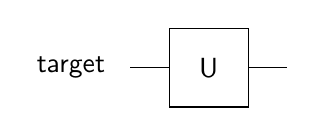
\begin{tikzpicture}[scale=.5] \node[draw=none] at (-3.5, 0) {target}; \draw (-2,0) -- (-1, 0); \draw (1, 0) -- (2, 0); \draw (-1,-1)--(-1,1)--(1,1)--(1,-1)--cycle; \node[draw=none] at (0, 0) {U}; \end{tikzpicture} } \]


\begin{DoxyParams}[1]{Parameters}
\mbox{\tt in,out}  & {\em multi\+Qubit} & object representing the set of all qubits \\
\hline
\mbox{\tt in}  & {\em target\+Qubit} & qubit to operate on \\
\hline
\mbox{\tt in}  & {\em alpha} & complex unitary parameter (row 1, column 1) \\
\hline
\mbox{\tt in}  & {\em beta} & complex unitary parameter (row 2, column 1) \\
\hline
\end{DoxyParams}

\begin{DoxyExceptions}{Exceptions}
{\em exit\+With\+Error} & if {\ttfamily target\+Qubit} is outside \mbox{[}0, {\ttfamily multi\+Qubit.\+num\+Qubits}), or if {\ttfamily alpha}, {\ttfamily beta} don\textquotesingle{}t satisfy $\vert${\ttfamily alpha$\vert$$^\wedge$2} + $\vert${\ttfamily beta$\vert$$^\wedge$2} = 1. \\
\hline
\end{DoxyExceptions}


Definition at line 98 of file Qu\+E\+S\+T\+\_\+env\+\_\+local.\+c.



References Multi\+Qubit\+::chunk\+Id, chunk\+Is\+Upper(), compact\+Unitary\+Distributed(), compact\+Unitary\+Local(), exchange\+State\+Vectors(), get\+Chunk\+Pair\+Id(), get\+Rot\+Angle(), half\+Matrix\+Block\+Fits\+In\+Chunk(), Multi\+Qubit\+::num\+Amps\+Per\+Chunk, Multi\+Qubit\+::num\+Qubits, Multi\+Qubit\+::pair\+State\+Vec, Qu\+E\+S\+T\+Assert(), R\+E\+AL, Multi\+Qubit\+::state\+Vec, and validate\+Alpha\+Beta().



Referenced by main(), rotate\+Around\+Axis(), test\+\_\+compact\+Unitary(), and test\+\_\+unitary().


\begin{DoxyCode}
99 \{
100     \mbox{\hyperlink{QuEST__env__local_8c_a3587b9d533e633ccf1abf9ad2ce45d8d}{QuESTAssert}}(targetQubit >= 0 && targetQubit < multiQubit.
      \mbox{\hyperlink{structMultiQubit_ab5b9795bdc6fb5855e1974dcbbaeb36f}{numQubits}}, 1, \_\_func\_\_);
101     \mbox{\hyperlink{QuEST__env__local_8c_a3587b9d533e633ccf1abf9ad2ce45d8d}{QuESTAssert}}(\mbox{\hyperlink{QuEST_8c_ae2b2c14a07dd7d50ff86032a3ca101d7}{validateAlphaBeta}}(alpha, beta), 6, \_\_func\_\_);
102 
103     \textcolor{comment}{// all values required to update state vector lie in this rank}
104     \mbox{\hyperlink{QuEST_8c_a9cee2d8716667a3318420a3b672f5b92}{compactUnitaryLocal}}(multiQubit, targetQubit, alpha, beta);
105 \}
\end{DoxyCode}
\mbox{\Hypertarget{QuEST_8h_ab4812953bc457405b3aa05a4c2f64f4a}\label{QuEST_8h_ab4812953bc457405b3aa05a4c2f64f4a}} 
\index{Qu\+E\+S\+T.\+h@{Qu\+E\+S\+T.\+h}!controlled\+Compact\+Unitary@{controlled\+Compact\+Unitary}}
\index{controlled\+Compact\+Unitary@{controlled\+Compact\+Unitary}!Qu\+E\+S\+T.\+h@{Qu\+E\+S\+T.\+h}}
\paragraph{\texorpdfstring{controlled\+Compact\+Unitary()}{controlledCompactUnitary()}}
{\footnotesize\ttfamily void controlled\+Compact\+Unitary (\begin{DoxyParamCaption}\item[{\mbox{\hyperlink{structMultiQubit}{Multi\+Qubit}}}]{multi\+Qubit,  }\item[{const int}]{control\+Qubit,  }\item[{const int}]{target\+Qubit,  }\item[{\mbox{\hyperlink{structComplex}{Complex}}}]{alpha,  }\item[{\mbox{\hyperlink{structComplex}{Complex}}}]{beta }\end{DoxyParamCaption})}



Apply a controlled unitary (single control, single target) parameterised by two given complex scalars. 

Given valid complex numbers $\alpha$ and $\beta$, applies the two-\/qubit unitary \[ \begin{pmatrix} 1 \\ & 1 \\ & & \alpha & -\beta^* \\ & & \beta & \alpha^* \end{pmatrix} \] to the control and target qubits. Valid $\alpha$, $\beta$ satisfy $|\alpha|^2 + |\beta|^2 = 1$. The target unitary is general up to a global phase factor. ~\newline
 \[ \setlength{\fboxrule}{0.01pt} \fbox{ 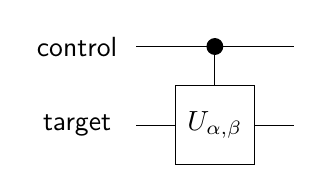
\begin{tikzpicture}[scale=.5] \node[draw=none] at (-3.5, 2) {control}; \node[draw=none] at (-3.5, 0) {target}; \draw (-2, 2) -- (2, 2); \draw[fill=black] (0, 2) circle (.2); \draw (0, 2) -- (0, 1); \draw (-2,0) -- (-1, 0); \draw (1, 0) -- (2, 0); \draw (-1,-1)--(-1,1)--(1,1)--(1,-1)--cycle; \node[draw=none] at (0, 0) {$U_{\alpha, \beta}$}; \end{tikzpicture} } \]


\begin{DoxyParams}[1]{Parameters}
\mbox{\tt in,out}  & {\em multi\+Qubit} & object representing the set of all qubits \\
\hline
\mbox{\tt in}  & {\em control\+Qubit} & apply the target unitary if this qubit has value 1 \\
\hline
\mbox{\tt in}  & {\em target\+Qubit} & qubit on which to apply the target unitary \\
\hline
\mbox{\tt in}  & {\em alpha} & complex unitary parameter (row 1, column 1) \\
\hline
\mbox{\tt in}  & {\em beta} & complex unitary parameter (row 2, column 1) \\
\hline
\end{DoxyParams}

\begin{DoxyExceptions}{Exceptions}
{\em exit\+With\+Error} & if either {\ttfamily control\+Qubit} or {\ttfamily target\+Qubit} are outside \mbox{[}0, {\ttfamily multi\+Qubit.\+num\+Qubits}) or are equal, or if {\ttfamily alpha}, {\ttfamily beta} don\textquotesingle{}t satisfy $\vert${\ttfamily alpha$\vert$$^\wedge$2} + $\vert${\ttfamily beta$\vert$$^\wedge$2} = 1. \\
\hline
\end{DoxyExceptions}


Definition at line 116 of file Qu\+E\+S\+T\+\_\+env\+\_\+local.\+c.



References Multi\+Qubit\+::chunk\+Id, chunk\+Is\+Upper(), controlled\+Compact\+Unitary\+Distributed(), controlled\+Compact\+Unitary\+Local(), exchange\+State\+Vectors(), get\+Chunk\+Pair\+Id(), get\+Rot\+Angle(), half\+Matrix\+Block\+Fits\+In\+Chunk(), Multi\+Qubit\+::num\+Amps\+Per\+Chunk, Multi\+Qubit\+::num\+Qubits, Multi\+Qubit\+::pair\+State\+Vec, Qu\+E\+S\+T\+Assert(), R\+E\+AL, Multi\+Qubit\+::state\+Vec, and validate\+Alpha\+Beta().



Referenced by controlled\+Rotate\+Around\+Axis(), main(), test\+\_\+controlled\+Compact\+Unitary(), test\+\_\+controlled\+Unitary(), and test\+\_\+multi\+Controlled\+Unitary().


\begin{DoxyCode}
117 \{
118     \mbox{\hyperlink{QuEST__env__local_8c_a3587b9d533e633ccf1abf9ad2ce45d8d}{QuESTAssert}}(targetQubit >= 0 && targetQubit < multiQubit.
      \mbox{\hyperlink{structMultiQubit_ab5b9795bdc6fb5855e1974dcbbaeb36f}{numQubits}}, 1, \_\_func\_\_);
119     \mbox{\hyperlink{QuEST__env__local_8c_a3587b9d533e633ccf1abf9ad2ce45d8d}{QuESTAssert}}(controlQubit >= 0 && controlQubit < multiQubit.
      \mbox{\hyperlink{structMultiQubit_ab5b9795bdc6fb5855e1974dcbbaeb36f}{numQubits}}, 2, \_\_func\_\_);
120     \mbox{\hyperlink{QuEST__env__local_8c_a3587b9d533e633ccf1abf9ad2ce45d8d}{QuESTAssert}}(controlQubit != targetQubit, 3, \_\_func\_\_);
121     \mbox{\hyperlink{QuEST__env__local_8c_a3587b9d533e633ccf1abf9ad2ce45d8d}{QuESTAssert}}(\mbox{\hyperlink{QuEST_8c_ae2b2c14a07dd7d50ff86032a3ca101d7}{validateAlphaBeta}}(alpha, beta), 6, \_\_func\_\_);
122 
123 
124     \mbox{\hyperlink{QuEST_8c_afc77657651d52c47403b44b923a098a8}{controlledCompactUnitaryLocal}}(multiQubit, controlQubit, targetQubit, alpha
      , beta);
125 \}
\end{DoxyCode}
\mbox{\Hypertarget{QuEST_8h_a67576895bbc65463481a8ea24d9b1e22}\label{QuEST_8h_a67576895bbc65463481a8ea24d9b1e22}} 
\index{Qu\+E\+S\+T.\+h@{Qu\+E\+S\+T.\+h}!controlled\+Not@{controlled\+Not}}
\index{controlled\+Not@{controlled\+Not}!Qu\+E\+S\+T.\+h@{Qu\+E\+S\+T.\+h}}
\paragraph{\texorpdfstring{controlled\+Not()}{controlledNot()}}
{\footnotesize\ttfamily void controlled\+Not (\begin{DoxyParamCaption}\item[{\mbox{\hyperlink{structMultiQubit}{Multi\+Qubit}}}]{multi\+Qubit,  }\item[{const int}]{control\+Qubit,  }\item[{const int}]{target\+Qubit }\end{DoxyParamCaption})}



Apply the controlled not (single control, single target) gate, also known as the c-\/X, c-\/sigma-\/X, c-\/\+Pauli-\/X and c-\/bit-\/flip gate. 

This applies sigmaX to the target qubit if the control qubit has value 1. This effects the two-\/qubit unitary \[ \begin{pmatrix} 1 \\ & 1 \\\ & & & 1 \\ & & 1 \end{pmatrix} \] on the control and target qubits.

\[ \setlength{\fboxrule}{0.01pt} \fbox{ 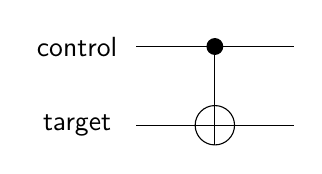
\begin{tikzpicture}[scale=.5] \node[draw=none] at (-3.5, 2) {control}; \node[draw=none] at (-3.5, 0) {target}; \draw (-2, 2) -- (2, 2); \draw[fill=black] (0, 2) circle (.2); \draw (0, 2) -- (0, -.5); \draw (-2,0) -- (2, 0); \draw (0, 0) circle (.5); \end{tikzpicture} } \] ~\newline
 
\begin{DoxyParams}[1]{Parameters}
\mbox{\tt in,out}  & {\em multi\+Qubit} & object representing the set of all qubits \\
\hline
\mbox{\tt in}  & {\em control\+Qubit} & nots the target if this qubit is 1 \\
\hline
\mbox{\tt in}  & {\em target\+Qubit} & qubit to not \\
\hline
\end{DoxyParams}

\begin{DoxyExceptions}{Exceptions}
{\em exit\+With\+Error} & if either {\ttfamily control\+Qubit} or {\ttfamily target\+Qubit} are outside \mbox{[}0, {\ttfamily multi\+Qubit.\+num\+Qubits}), or are equal. \\
\hline
\end{DoxyExceptions}


Definition at line 175 of file Qu\+E\+S\+T\+\_\+env\+\_\+local.\+c.



References Multi\+Qubit\+::chunk\+Id, chunk\+Is\+Upper(), controlled\+Not\+Distributed(), controlled\+Not\+Local(), exchange\+State\+Vectors(), get\+Chunk\+Pair\+Id(), half\+Matrix\+Block\+Fits\+In\+Chunk(), Multi\+Qubit\+::num\+Amps\+Per\+Chunk, Multi\+Qubit\+::num\+Qubits, Multi\+Qubit\+::pair\+State\+Vec, Qu\+E\+S\+T\+Assert(), R\+E\+AL, and Multi\+Qubit\+::state\+Vec.



Referenced by main(), and test\+\_\+controlled\+Not().


\begin{DoxyCode}
176 \{
177     \mbox{\hyperlink{QuEST__env__local_8c_a3587b9d533e633ccf1abf9ad2ce45d8d}{QuESTAssert}}(targetQubit >= 0 && targetQubit < multiQubit.
      \mbox{\hyperlink{structMultiQubit_ab5b9795bdc6fb5855e1974dcbbaeb36f}{numQubits}}, 1, \_\_func\_\_);
178     \mbox{\hyperlink{QuEST__env__local_8c_a3587b9d533e633ccf1abf9ad2ce45d8d}{QuESTAssert}}(controlQubit >= 0 && controlQubit < multiQubit.
      \mbox{\hyperlink{structMultiQubit_ab5b9795bdc6fb5855e1974dcbbaeb36f}{numQubits}}, 2, \_\_func\_\_);
179     \mbox{\hyperlink{QuEST__env__local_8c_a3587b9d533e633ccf1abf9ad2ce45d8d}{QuESTAssert}}(controlQubit != targetQubit, 3, \_\_func\_\_);
180     \mbox{\hyperlink{QuEST_8c_ad357a43e80e3baf013975b1b70942f4c}{controlledNotLocal}}(multiQubit, controlQubit, targetQubit);
181 \}
\end{DoxyCode}
\mbox{\Hypertarget{QuEST_8h_a11a96159191cbf1b01a1080e7f045aac}\label{QuEST_8h_a11a96159191cbf1b01a1080e7f045aac}} 
\index{Qu\+E\+S\+T.\+h@{Qu\+E\+S\+T.\+h}!controlled\+Phase\+Gate@{controlled\+Phase\+Gate}}
\index{controlled\+Phase\+Gate@{controlled\+Phase\+Gate}!Qu\+E\+S\+T.\+h@{Qu\+E\+S\+T.\+h}}
\paragraph{\texorpdfstring{controlled\+Phase\+Gate()}{controlledPhaseGate()}}
{\footnotesize\ttfamily void controlled\+Phase\+Gate (\begin{DoxyParamCaption}\item[{\mbox{\hyperlink{structMultiQubit}{Multi\+Qubit}}}]{multi\+Qubit,  }\item[{const int}]{id\+Qubit1,  }\item[{const int}]{id\+Qubit2 }\end{DoxyParamCaption})}



Apply the (two-\/qubit) controlled phase gate, also known as the controlled sigmaZ gate. 

For each state, if both input qubits have value one, multiply the amplitude of that state by -\/1. This applies the two-\/qubit unitary\+: \[ \begin{pmatrix} 1 \\ & 1 \\\ & & 1 \\ & & & -1 \end{pmatrix} \]

\[ \setlength{\fboxrule}{0.01pt} \fbox{ 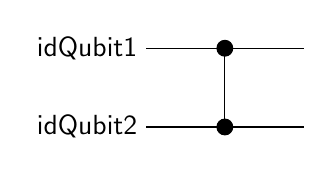
\begin{tikzpicture}[scale=.5] \node[draw=none] at (-3.5, 2) {idQubit1}; \node[draw=none] at (-3.5, 0) {idQubit2}; \draw (-2, 2) -- (2, 2); \draw[fill=black] (0, 2) circle (.2); \draw (0, 2) -- (0, 0); \draw (-2,0) -- (2, 0); \draw[fill=black] (0, 0) circle (.2); \end{tikzpicture} } \]


\begin{DoxyParams}[1]{Parameters}
\mbox{\tt in,out}  & {\em multi\+Qubit} & object representing the set of all qubits \\
\hline
\mbox{\tt in}  & {\em id\+Qubit1,id\+Qubit2} & qubits to operate upon \\
\hline
\end{DoxyParams}

\begin{DoxyExceptions}{Exceptions}
{\em exit\+With\+Error} & if {\ttfamily id\+Qubit1} or {\ttfamily id\+Qubit2} are outside \mbox{[}0, {\ttfamily multi\+Qubit.\+num\+Qubits}), or are equal \\
\hline
\end{DoxyExceptions}


Definition at line 1748 of file Qu\+E\+S\+T.\+c.



References Multi\+Qubit\+::chunk\+Id, extract\+Bit(), Complex\+Array\+::imag, Multi\+Qubit\+::num\+Amps\+Per\+Chunk, Multi\+Qubit\+::num\+Qubits, Qu\+E\+S\+T\+Assert(), Complex\+Array\+::real, R\+E\+AL, and Multi\+Qubit\+::state\+Vec.



Referenced by test\+\_\+controlled\+Phase\+Gate().


\begin{DoxyCode}
1749 \{
1750     \textcolor{keywordtype}{long} \textcolor{keywordtype}{long} \textcolor{keywordtype}{int} index;
1751     \textcolor{keywordtype}{long} \textcolor{keywordtype}{long} \textcolor{keywordtype}{int} stateVecSize;
1752     \textcolor{keywordtype}{int} bit1, bit2;
1753 
1754     \textcolor{keyword}{const} \textcolor{keywordtype}{long} \textcolor{keywordtype}{long} \textcolor{keywordtype}{int} chunkSize=multiQubit.\mbox{\hyperlink{structMultiQubit_a1cad83601a78635dd278259c7ed54f18}{numAmpsPerChunk}};
1755     \textcolor{keyword}{const} \textcolor{keywordtype}{long} \textcolor{keywordtype}{long} \textcolor{keywordtype}{int} chunkId=multiQubit.\mbox{\hyperlink{structMultiQubit_ab10c88249fa3825d6227ceec01d37e37}{chunkId}};
1756 
1757     \mbox{\hyperlink{QuEST__env__local_8c_a3587b9d533e633ccf1abf9ad2ce45d8d}{QuESTAssert}}(idQubit1 >= 0 && idQubit1 < multiQubit.\mbox{\hyperlink{structMultiQubit_ab5b9795bdc6fb5855e1974dcbbaeb36f}{numQubits}}, 2, \_\_func\_\_);
1758     \mbox{\hyperlink{QuEST__env__local_8c_a3587b9d533e633ccf1abf9ad2ce45d8d}{QuESTAssert}}(idQubit2 >= 0 && idQubit2 < multiQubit.\mbox{\hyperlink{structMultiQubit_ab5b9795bdc6fb5855e1974dcbbaeb36f}{numQubits}}, 1, \_\_func\_\_);
1759     \mbox{\hyperlink{QuEST__env__local_8c_a3587b9d533e633ccf1abf9ad2ce45d8d}{QuESTAssert}}(idQubit1 != idQubit2, 3, \_\_func\_\_);
1760 
1761     \textcolor{comment}{// dimension of the state vector}
1762     stateVecSize = multiQubit.\mbox{\hyperlink{structMultiQubit_a1cad83601a78635dd278259c7ed54f18}{numAmpsPerChunk}};
1763     \mbox{\hyperlink{QuEST__precision_8h_a4b654506f18b8bfd61ad2a29a7e38c25}{REAL}} *stateVecReal = multiQubit.\mbox{\hyperlink{structMultiQubit_a45483190d6b01ef6b2f98f2bec9ab94f}{stateVec}}.\mbox{\hyperlink{structComplexArray_a4195cac6c784ea1b6271f1c7dba1548a}{real}};
1764     \mbox{\hyperlink{QuEST__precision_8h_a4b654506f18b8bfd61ad2a29a7e38c25}{REAL}} *stateVecImag = multiQubit.\mbox{\hyperlink{structMultiQubit_a45483190d6b01ef6b2f98f2bec9ab94f}{stateVec}}.\mbox{\hyperlink{structComplexArray_a79dde47c7ae530c79cebfdf57b225968}{imag}};
1765 
1766 \textcolor{preprocessor}{# ifdef \_OPENMP}
1767 \textcolor{preprocessor}{# pragma omp parallel for \(\backslash\)}
1768 \textcolor{preprocessor}{    default  (none)                          \(\backslash\)}
1769 \textcolor{preprocessor}{    shared   (stateVecSize, stateVecReal,stateVecImag ) \(\backslash\)}
1770 \textcolor{preprocessor}{    private  (index,bit1,bit2)                 \(\backslash\)}
1771 \textcolor{preprocessor}{    schedule (static)}
1772 \textcolor{preprocessor}{# endif}
1773     \textcolor{keywordflow}{for} (index=0; index<stateVecSize; index++) \{
1774         bit1 = \mbox{\hyperlink{QuEST_8c_a100463f6ec212c76a5fad99579000505}{extractBit}} (idQubit1, index+chunkId*chunkSize);
1775         bit2 = \mbox{\hyperlink{QuEST_8c_a100463f6ec212c76a5fad99579000505}{extractBit}} (idQubit2, index+chunkId*chunkSize);
1776         \textcolor{keywordflow}{if} (bit1 && bit2) \{
1777             stateVecReal [index] = - stateVecReal [index];
1778             stateVecImag [index] = - stateVecImag [index];
1779         \}
1780     \}
1781 \}
\end{DoxyCode}
\mbox{\Hypertarget{QuEST_8h_ad41f82b41149393a642391b67b3a287e}\label{QuEST_8h_ad41f82b41149393a642391b67b3a287e}} 
\index{Qu\+E\+S\+T.\+h@{Qu\+E\+S\+T.\+h}!controlled\+Rotate\+Around\+Axis@{controlled\+Rotate\+Around\+Axis}}
\index{controlled\+Rotate\+Around\+Axis@{controlled\+Rotate\+Around\+Axis}!Qu\+E\+S\+T.\+h@{Qu\+E\+S\+T.\+h}}
\paragraph{\texorpdfstring{controlled\+Rotate\+Around\+Axis()}{controlledRotateAroundAxis()}}
{\footnotesize\ttfamily void controlled\+Rotate\+Around\+Axis (\begin{DoxyParamCaption}\item[{\mbox{\hyperlink{structMultiQubit}{Multi\+Qubit}}}]{multi\+Qubit,  }\item[{const int}]{control\+Qubit,  }\item[{const int}]{target\+Qubit,  }\item[{\mbox{\hyperlink{QuEST__precision_8h_a4b654506f18b8bfd61ad2a29a7e38c25}{R\+E\+AL}}}]{angle,  }\item[{\mbox{\hyperlink{structVector}{Vector}}}]{axis }\end{DoxyParamCaption})}



Applies a controlled rotation by a given angle around a given vector on the Bloch-\/sphere. 

The vector must not be zero (else an error is thrown), but needn\textquotesingle{}t be unit magnitude.

For angle $\theta$ and axis vector $\vec{n}$, applies $R_{\hat{n}} = \exp \left(- i \frac{\theta}{2} \hat{n} \cdot \vec{\sigma} \right) $ to states where the target qubit is 1 ( $\vec{\sigma}$ is the vector of Pauli matrices).

\[ \setlength{\fboxrule}{0.01pt} \fbox{ 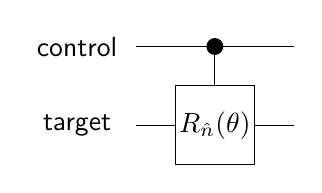
\begin{tikzpicture}[scale=.5] \node[draw=none] at (-3.5, 2) {control}; \node[draw=none] at (-3.5, 0) {target}; \draw (-2, 2) -- (2, 2); \draw[fill=black] (0, 2) circle (.2); \draw (0, 2) -- (0, 1); \draw (-2,0) -- (-1, 0); \draw (1, 0) -- (2, 0); \draw (-1,-1)--(-1,1)--(1,1)--(1,-1)--cycle; \node[draw=none] at (0, 0) {$R_{\hat{n}}(\theta)$}; \end{tikzpicture} } \]


\begin{DoxyParams}[1]{Parameters}
\mbox{\tt in,out}  & {\em multi\+Qubit} & object representing the set of all qubits \\
\hline
\mbox{\tt in}  & {\em control\+Qubit} & qubit with value 1 in the rotated states \\
\hline
\mbox{\tt in}  & {\em target\+Qubit} & qubit to rotate \\
\hline
\mbox{\tt in}  & {\em angle} & angle by which to rotate in radians \\
\hline
\mbox{\tt in}  & {\em axis} & vector around which to rotate (can be non-\/unit; will be normalised) \\
\hline
\end{DoxyParams}

\begin{DoxyExceptions}{Exceptions}
{\em exit\+With\+Error} & if either {\ttfamily control\+Qubit} or {\ttfamily target\+Qubit} are outside \mbox{[}0, {\ttfamily multi\+Qubit.\+num\+Qubits}) or are equal or if {\ttfamily axis} is the zero vector \\
\hline
\end{DoxyExceptions}


Definition at line 459 of file Qu\+E\+S\+T.\+c.



References controlled\+Compact\+Unitary(), Complex\+::imag, Complex\+::real, Vector\+::x, Vector\+::y, and Vector\+::z.



Referenced by controlled\+Rotate\+X(), controlled\+Rotate\+Y(), and controlled\+Rotate\+Z().


\begin{DoxyCode}
459                                                                                                            
                         \{
460 
461     \textcolor{keywordtype}{double} mag = sqrt(pow(axis.\mbox{\hyperlink{structVector_aac7abe171ba4bada50ed72acba6259fc}{x}},2) + pow(axis.\mbox{\hyperlink{structVector_a375ca805d4c808a53d7c4e0c737ae3de}{y}},2) + pow(axis.\mbox{\hyperlink{structVector_ad4e863651be7d6b7e2b28cd7445a0ccf}{z}},2));
462     \mbox{\hyperlink{structVector}{Vector}} unitAxis = \{axis.\mbox{\hyperlink{structVector_aac7abe171ba4bada50ed72acba6259fc}{x}}/mag, axis.\mbox{\hyperlink{structVector_a375ca805d4c808a53d7c4e0c737ae3de}{y}}/mag, axis.\mbox{\hyperlink{structVector_ad4e863651be7d6b7e2b28cd7445a0ccf}{z}}/mag\};
463 
464     \mbox{\hyperlink{structComplex}{Complex}} alpha, beta;
465     alpha.\mbox{\hyperlink{structComplex_a479ad939835457595fcca3ca55c06283}{real}} = cos(angle/2.0);
466     alpha.\mbox{\hyperlink{structComplex_a1151948284b21c0052f203f23ab931d9}{imag}} = -sin(angle/2.0)*unitAxis.\mbox{\hyperlink{structVector_ad4e863651be7d6b7e2b28cd7445a0ccf}{z}};       
467     beta.\mbox{\hyperlink{structComplex_a479ad939835457595fcca3ca55c06283}{real}} = sin(angle/2.0)*unitAxis.\mbox{\hyperlink{structVector_a375ca805d4c808a53d7c4e0c737ae3de}{y}};
468     beta.\mbox{\hyperlink{structComplex_a1151948284b21c0052f203f23ab931d9}{imag}} = -sin(angle/2.0)*unitAxis.\mbox{\hyperlink{structVector_aac7abe171ba4bada50ed72acba6259fc}{x}};
469     \mbox{\hyperlink{QuEST__env__local_8c_ab4812953bc457405b3aa05a4c2f64f4a}{controlledCompactUnitary}}(multiQubit, controlQubit, targetQubit, alpha, beta);
470 \}
\end{DoxyCode}
\mbox{\Hypertarget{QuEST_8h_ac6923ac57e67d9a21096e06f6a9012f6}\label{QuEST_8h_ac6923ac57e67d9a21096e06f6a9012f6}} 
\index{Qu\+E\+S\+T.\+h@{Qu\+E\+S\+T.\+h}!controlled\+RotateX@{controlled\+RotateX}}
\index{controlled\+RotateX@{controlled\+RotateX}!Qu\+E\+S\+T.\+h@{Qu\+E\+S\+T.\+h}}
\paragraph{\texorpdfstring{controlled\+Rotate\+X()}{controlledRotateX()}}
{\footnotesize\ttfamily void controlled\+RotateX (\begin{DoxyParamCaption}\item[{\mbox{\hyperlink{structMultiQubit}{Multi\+Qubit}}}]{multi\+Qubit,  }\item[{const int}]{control\+Qubit,  }\item[{const int}]{target\+Qubit,  }\item[{\mbox{\hyperlink{QuEST__precision_8h_a4b654506f18b8bfd61ad2a29a7e38c25}{R\+E\+AL}}}]{angle }\end{DoxyParamCaption})}



Applies a controlled rotation by a given angle around the X-\/axis of the Bloch-\/sphere. 

The target qubit is rotated in states where the control qubit has value 1.

\[ \setlength{\fboxrule}{0.01pt} \fbox{ 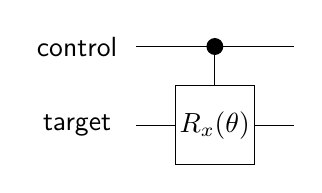
\begin{tikzpicture}[scale=.5] \node[draw=none] at (-3.5, 2) {control}; \node[draw=none] at (-3.5, 0) {target}; \draw (-2, 2) -- (2, 2); \draw[fill=black] (0, 2) circle (.2); \draw (0, 2) -- (0, 1); \draw (-2,0) -- (-1, 0); \draw (1, 0) -- (2, 0); \draw (-1,-1)--(-1,1)--(1,1)--(1,-1)--cycle; \node[draw=none] at (0, 0) {$R_x(\theta)$}; \end{tikzpicture} } \] ~\newline
 
\begin{DoxyParams}[1]{Parameters}
\mbox{\tt in,out}  & {\em multi\+Qubit} & object representing the set of all qubits \\
\hline
\mbox{\tt in}  & {\em control\+Qubit} & qubit which has value 1 in the rotated states \\
\hline
\mbox{\tt in}  & {\em tagret\+Qubit} & qubit to rotate \\
\hline
\mbox{\tt in}  & {\em angle} & angle by which to rotate the target qubit in radians \\
\hline
\end{DoxyParams}

\begin{DoxyExceptions}{Exceptions}
{\em exit\+With\+Error} & if either {\ttfamily control\+Qubit} or {\ttfamily target\+Qubit} are outside \mbox{[}0, {\ttfamily multi\+Qubit.\+num\+Qubits}) or are equal. \\
\hline
\end{DoxyExceptions}


Definition at line 472 of file Qu\+E\+S\+T.\+c.



References controlled\+Rotate\+Around\+Axis().


\begin{DoxyCode}
472                                                                                                         \{
473 
474     \mbox{\hyperlink{structVector}{Vector}} unitAxis = \{1, 0, 0\};
475     \mbox{\hyperlink{QuEST_8c_ad41f82b41149393a642391b67b3a287e}{controlledRotateAroundAxis}}(multiQubit, controlQubit, targetQubit, angle, 
      unitAxis);
476 \}
\end{DoxyCode}
\mbox{\Hypertarget{QuEST_8h_a71e90a2f7292116338c062934f9d1202}\label{QuEST_8h_a71e90a2f7292116338c062934f9d1202}} 
\index{Qu\+E\+S\+T.\+h@{Qu\+E\+S\+T.\+h}!controlled\+RotateY@{controlled\+RotateY}}
\index{controlled\+RotateY@{controlled\+RotateY}!Qu\+E\+S\+T.\+h@{Qu\+E\+S\+T.\+h}}
\paragraph{\texorpdfstring{controlled\+Rotate\+Y()}{controlledRotateY()}}
{\footnotesize\ttfamily void controlled\+RotateY (\begin{DoxyParamCaption}\item[{\mbox{\hyperlink{structMultiQubit}{Multi\+Qubit}}}]{multi\+Qubit,  }\item[{const int}]{control\+Qubit,  }\item[{const int}]{target\+Qubit,  }\item[{\mbox{\hyperlink{QuEST__precision_8h_a4b654506f18b8bfd61ad2a29a7e38c25}{R\+E\+AL}}}]{angle }\end{DoxyParamCaption})}



Applies a controlled rotation by a given angle around the Y-\/axis of the Bloch-\/sphere. 

The target qubit is rotated in states where the control qubit has value 1.

\[ \setlength{\fboxrule}{0.01pt} \fbox{ 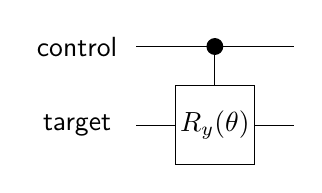
\begin{tikzpicture}[scale=.5] \node[draw=none] at (-3.5, 2) {control}; \node[draw=none] at (-3.5, 0) {target}; \draw (-2, 2) -- (2, 2); \draw[fill=black] (0, 2) circle (.2); \draw (0, 2) -- (0, 1); \draw (-2,0) -- (-1, 0); \draw (1, 0) -- (2, 0); \draw (-1,-1)--(-1,1)--(1,1)--(1,-1)--cycle; \node[draw=none] at (0, 0) {$R_y(\theta)$}; \end{tikzpicture} } \] ~\newline
 
\begin{DoxyParams}[1]{Parameters}
\mbox{\tt in,out}  & {\em multi\+Qubit} & object representing the set of all qubits \\
\hline
\mbox{\tt in}  & {\em control\+Qubit} & qubit which has value 1 in the rotated states \\
\hline
\mbox{\tt in}  & {\em tagret\+Qubit} & qubit to rotate \\
\hline
\mbox{\tt in}  & {\em angle} & angle by which to rotate the target qubit in radians \\
\hline
\end{DoxyParams}

\begin{DoxyExceptions}{Exceptions}
{\em exit\+With\+Error} & if either {\ttfamily control\+Qubit} or {\ttfamily target\+Qubit} are outside \mbox{[}0, {\ttfamily multi\+Qubit.\+num\+Qubits}) or are equal. \\
\hline
\end{DoxyExceptions}


Definition at line 478 of file Qu\+E\+S\+T.\+c.



References controlled\+Rotate\+Around\+Axis().


\begin{DoxyCode}
478                                                                                                         \{
479 
480     \mbox{\hyperlink{structVector}{Vector}} unitAxis = \{0, 1, 0\};
481     \mbox{\hyperlink{QuEST_8c_ad41f82b41149393a642391b67b3a287e}{controlledRotateAroundAxis}}(multiQubit, controlQubit, targetQubit, angle, 
      unitAxis);
482 \}
\end{DoxyCode}
\mbox{\Hypertarget{QuEST_8h_a668e5d2634b02e98bc73675ccb11d61c}\label{QuEST_8h_a668e5d2634b02e98bc73675ccb11d61c}} 
\index{Qu\+E\+S\+T.\+h@{Qu\+E\+S\+T.\+h}!controlled\+RotateZ@{controlled\+RotateZ}}
\index{controlled\+RotateZ@{controlled\+RotateZ}!Qu\+E\+S\+T.\+h@{Qu\+E\+S\+T.\+h}}
\paragraph{\texorpdfstring{controlled\+Rotate\+Z()}{controlledRotateZ()}}
{\footnotesize\ttfamily void controlled\+RotateZ (\begin{DoxyParamCaption}\item[{\mbox{\hyperlink{structMultiQubit}{Multi\+Qubit}}}]{multi\+Qubit,  }\item[{const int}]{control\+Qubit,  }\item[{const int}]{target\+Qubit,  }\item[{\mbox{\hyperlink{QuEST__precision_8h_a4b654506f18b8bfd61ad2a29a7e38c25}{R\+E\+AL}}}]{angle }\end{DoxyParamCaption})}



Applies a controlled rotation by a given angle around the Z-\/axis of the Bloch-\/sphere. 

The target qubit is rotated in states where the control qubit has value 1.

\[ \setlength{\fboxrule}{0.01pt} \fbox{ 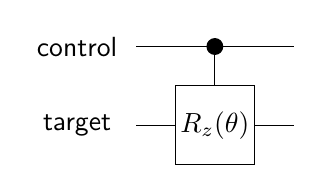
\begin{tikzpicture}[scale=.5] \node[draw=none] at (-3.5, 2) {control}; \node[draw=none] at (-3.5, 0) {target}; \draw (-2, 2) -- (2, 2); \draw[fill=black] (0, 2) circle (.2); \draw (0, 2) -- (0, 1); \draw (-2,0) -- (-1, 0); \draw (1, 0) -- (2, 0); \draw (-1,-1)--(-1,1)--(1,1)--(1,-1)--cycle; \node[draw=none] at (0, 0) {$R_z(\theta)$}; \end{tikzpicture} } \] ~\newline
 
\begin{DoxyParams}[1]{Parameters}
\mbox{\tt in,out}  & {\em multi\+Qubit} & object representing the set of all qubits \\
\hline
\mbox{\tt in}  & {\em control\+Qubit} & qubit which has value 1 in the rotated states \\
\hline
\mbox{\tt in}  & {\em tagret\+Qubit} & qubit to rotate \\
\hline
\mbox{\tt in}  & {\em angle} & angle by which to rotate the target qubit in radians \\
\hline
\end{DoxyParams}

\begin{DoxyExceptions}{Exceptions}
{\em exit\+With\+Error} & if either {\ttfamily control\+Qubit} or {\ttfamily target\+Qubit} are outside \mbox{[}0, {\ttfamily multi\+Qubit.\+num\+Qubits}) or are equal. \\
\hline
\end{DoxyExceptions}


Definition at line 484 of file Qu\+E\+S\+T.\+c.



References controlled\+Rotate\+Around\+Axis().


\begin{DoxyCode}
484                                                                                                         \{
485 
486     \mbox{\hyperlink{structVector}{Vector}} unitAxis = \{0, 0, 1\};
487     \mbox{\hyperlink{QuEST_8c_ad41f82b41149393a642391b67b3a287e}{controlledRotateAroundAxis}}(multiQubit, controlQubit, targetQubit, angle, 
      unitAxis);
488 \}
\end{DoxyCode}
\mbox{\Hypertarget{QuEST_8h_a8a701526263392599aa21d0d0f05d9d8}\label{QuEST_8h_a8a701526263392599aa21d0d0f05d9d8}} 
\index{Qu\+E\+S\+T.\+h@{Qu\+E\+S\+T.\+h}!controlled\+Unitary@{controlled\+Unitary}}
\index{controlled\+Unitary@{controlled\+Unitary}!Qu\+E\+S\+T.\+h@{Qu\+E\+S\+T.\+h}}
\paragraph{\texorpdfstring{controlled\+Unitary()}{controlledUnitary()}}
{\footnotesize\ttfamily void controlled\+Unitary (\begin{DoxyParamCaption}\item[{\mbox{\hyperlink{structMultiQubit}{Multi\+Qubit}}}]{multi\+Qubit,  }\item[{const int}]{control\+Qubit,  }\item[{const int}]{target\+Qubit,  }\item[{\mbox{\hyperlink{structComplexMatrix2}{Complex\+Matrix2}}}]{u }\end{DoxyParamCaption})}



Apply a general controlled unitary (single control, single target), which can include a global phase factor. 

The given unitary is applied to the target qubit if the control qubit has value 1, effecting the two-\/qubit unitary \[ \begin{pmatrix} 1 \\ & 1 \\ & & u_{00} & u_{01}\\ & & u_{10} & u_{11} \end{pmatrix} \] on the control and target qubits.

\[ \setlength{\fboxrule}{0.01pt} \fbox{ 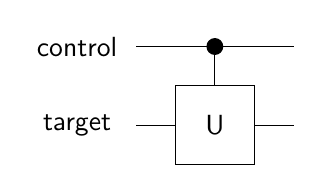
\begin{tikzpicture}[scale=.5] \node[draw=none] at (-3.5, 2) {control}; \node[draw=none] at (-3.5, 0) {target}; \draw (-2, 2) -- (2, 2); \draw[fill=black] (0, 2) circle (.2); \draw (0, 2) -- (0, 1); \draw (-2,0) -- (-1, 0); \draw (1, 0) -- (2, 0); \draw (-1,-1)--(-1,1)--(1,1)--(1,-1)--cycle; \node[draw=none] at (0, 0) {U}; \end{tikzpicture} } \]


\begin{DoxyParams}[1]{Parameters}
\mbox{\tt in,out}  & {\em multi\+Qubit} & object representing the set of all qubits \\
\hline
\mbox{\tt in}  & {\em control\+Qubit} & apply unitary if this qubit is 1 \\
\hline
\mbox{\tt in}  & {\em target\+Qubit} & qubit to operate on \\
\hline
\mbox{\tt in}  & {\em u} & single-\/qubit unitary matrix to apply \\
\hline
\end{DoxyParams}

\begin{DoxyExceptions}{Exceptions}
{\em exit\+With\+Error} & if either {\ttfamily control\+Qubit} or {\ttfamily target\+Qubit} are outside \mbox{[}0, {\ttfamily multi\+Qubit.\+num\+Qubits}) or are equal, or if {\ttfamily u} is not unitary. \\
\hline
\end{DoxyExceptions}


Definition at line 127 of file Qu\+E\+S\+T\+\_\+env\+\_\+local.\+c.



References Multi\+Qubit\+::chunk\+Id, chunk\+Is\+Upper(), controlled\+Unitary\+Distributed(), controlled\+Unitary\+Local(), exchange\+State\+Vectors(), get\+Chunk\+Pair\+Id(), get\+Rot\+Angle\+From\+Unitary\+Matrix(), half\+Matrix\+Block\+Fits\+In\+Chunk(), Multi\+Qubit\+::num\+Amps\+Per\+Chunk, Multi\+Qubit\+::num\+Qubits, Multi\+Qubit\+::pair\+State\+Vec, Qu\+E\+S\+T\+Assert(), R\+E\+AL, Multi\+Qubit\+::state\+Vec, and validate\+Matrix\+Is\+Unitary().



Referenced by test\+\_\+controlled\+Unitary().


\begin{DoxyCode}
128 \{
129     \mbox{\hyperlink{QuEST__env__local_8c_a3587b9d533e633ccf1abf9ad2ce45d8d}{QuESTAssert}}(targetQubit >= 0 && targetQubit < multiQubit.
      \mbox{\hyperlink{structMultiQubit_ab5b9795bdc6fb5855e1974dcbbaeb36f}{numQubits}}, 1, \_\_func\_\_);
130     \mbox{\hyperlink{QuEST__env__local_8c_a3587b9d533e633ccf1abf9ad2ce45d8d}{QuESTAssert}}(controlQubit >= 0 && controlQubit < multiQubit.
      \mbox{\hyperlink{structMultiQubit_ab5b9795bdc6fb5855e1974dcbbaeb36f}{numQubits}}, 2, \_\_func\_\_);
131     \mbox{\hyperlink{QuEST__env__local_8c_a3587b9d533e633ccf1abf9ad2ce45d8d}{QuESTAssert}}(controlQubit != targetQubit, 3, \_\_func\_\_);
132     \mbox{\hyperlink{QuEST__env__local_8c_a3587b9d533e633ccf1abf9ad2ce45d8d}{QuESTAssert}}(\mbox{\hyperlink{QuEST_8c_ae4fea133d1a8f09ff8da03038100adb2}{validateMatrixIsUnitary}}(u), 5, \_\_func\_\_);
133 
134     \mbox{\hyperlink{QuEST_8c_a8a4afcff70195a306c082b8ed8d4e09a}{controlledUnitaryLocal}}(multiQubit, controlQubit, targetQubit, u);
135 \}
\end{DoxyCode}
\mbox{\Hypertarget{QuEST_8h_a9c02591bc64c2918503afa231d90d83f}\label{QuEST_8h_a9c02591bc64c2918503afa231d90d83f}} 
\index{Qu\+E\+S\+T.\+h@{Qu\+E\+S\+T.\+h}!create\+Multi\+Qubit@{create\+Multi\+Qubit}}
\index{create\+Multi\+Qubit@{create\+Multi\+Qubit}!Qu\+E\+S\+T.\+h@{Qu\+E\+S\+T.\+h}}
\paragraph{\texorpdfstring{create\+Multi\+Qubit()}{createMultiQubit()}}
{\footnotesize\ttfamily void create\+Multi\+Qubit (\begin{DoxyParamCaption}\item[{\mbox{\hyperlink{structMultiQubit}{Multi\+Qubit}} $\ast$}]{multi\+Qubit,  }\item[{int}]{num\+Qubits,  }\item[{\mbox{\hyperlink{structQuESTEnv}{Qu\+E\+S\+T\+Env}}}]{env }\end{DoxyParamCaption})}



Create a \mbox{\hyperlink{structMultiQubit}{Multi\+Qubit}} object representing a set of qubits. 

Allocate space for state vector of probability amplitudes, including space for temporary values to be copied from one other chunk if running the distributed version. Define properties related to the size of the set of qubits. init\+State\+Zero should be called after this to initialise the qubits to the zero state.


\begin{DoxyParams}[1]{Parameters}
\mbox{\tt in,out}  & {\em multi\+Qubit} & a pointer to an object representing the set of qubits \\
\hline
\mbox{\tt in}  & {\em num\+Qubits} & number of qubits in the system \\
\hline
\mbox{\tt in}  & {\em env} & object representing the execution environment (local, multinode etc) \\
\hline
\end{DoxyParams}

\begin{DoxyExceptions}{Exceptions}
{\em exit\+With\+Error} & if {\ttfamily num\+Qubits} $<$= 0 \\
\hline
\end{DoxyExceptions}


Definition at line 44 of file Qu\+E\+S\+T.\+c.



References Multi\+Qubit\+::chunk\+Id, Multi\+Qubit\+::device\+State\+Vec, env, Multi\+Qubit\+::first\+Level\+Reduction, Complex\+Array\+::imag, Multi\+Qubit\+::num\+Amps\+Per\+Chunk, Multi\+Qubit\+::num\+Chunks, Multi\+Qubit\+::num\+Qubits, Qu\+E\+S\+T\+Env\+::num\+Ranks, Multi\+Qubit\+::pair\+State\+Vec, Qu\+E\+S\+T\+Assert(), Qu\+E\+S\+T\+Env\+::rank, Complex\+Array\+::real, R\+E\+AL, R\+E\+D\+U\+C\+E\+\_\+\+S\+H\+A\+R\+E\+D\+\_\+\+S\+I\+ZE, Multi\+Qubit\+::second\+Level\+Reduction, and Multi\+Qubit\+::state\+Vec.



Referenced by main(), test\+\_\+collapse\+To\+Outcome(), test\+\_\+compact\+Unitary(), test\+\_\+controlled\+Compact\+Unitary(), test\+\_\+controlled\+Not(), test\+\_\+controlled\+Phase\+Gate(), test\+\_\+controlled\+Unitary(), test\+\_\+find\+Probability\+Of\+Outcome(), test\+\_\+get\+Imag\+Amp\+El(), test\+\_\+get\+Prob\+El(), test\+\_\+get\+Real\+Amp\+El(), test\+\_\+hadamard(), test\+\_\+init\+Classical\+State(), test\+\_\+init\+State\+Plus(), test\+\_\+init\+State\+Zero(), test\+\_\+measure(), test\+\_\+measure\+With\+Stats(), test\+\_\+multi\+Controlled\+Phase\+Gate(), test\+\_\+multi\+Controlled\+Unitary(), test\+\_\+s\+Gate(), test\+\_\+sigma\+X(), test\+\_\+sigma\+Y(), test\+\_\+sigma\+Z(), test\+\_\+t\+Gate(), and test\+\_\+unitary().


\begin{DoxyCode}
45 \{
46     \mbox{\hyperlink{QuEST__env__local_8c_a3587b9d533e633ccf1abf9ad2ce45d8d}{QuESTAssert}}(numQubits>0, 9, \_\_func\_\_);
47     \textcolor{keywordtype}{long} \textcolor{keywordtype}{long} \textcolor{keywordtype}{int} numAmps = 1L << numQubits;
48     \textcolor{keywordtype}{long} \textcolor{keywordtype}{long} \textcolor{keywordtype}{int} numAmpsPerRank = numAmps/\mbox{\hyperlink{runTests_8c_a5fd8ba97fcae3408ae6221dfc3cc1f93}{env}}.\mbox{\hyperlink{structQuESTEnv_af22aacd7c9905accae28484785c193b4}{numRanks}};
49 
50     multiQubit->\mbox{\hyperlink{structMultiQubit_a45483190d6b01ef6b2f98f2bec9ab94f}{stateVec}}.\mbox{\hyperlink{structComplexArray_a4195cac6c784ea1b6271f1c7dba1548a}{real}} = malloc(numAmpsPerRank * \textcolor{keyword}{sizeof}(*(multiQubit->
      \mbox{\hyperlink{structMultiQubit_a45483190d6b01ef6b2f98f2bec9ab94f}{stateVec}}.\mbox{\hyperlink{structComplexArray_a4195cac6c784ea1b6271f1c7dba1548a}{real}})));
51     multiQubit->\mbox{\hyperlink{structMultiQubit_a45483190d6b01ef6b2f98f2bec9ab94f}{stateVec}}.\mbox{\hyperlink{structComplexArray_a79dde47c7ae530c79cebfdf57b225968}{imag}} = malloc(numAmpsPerRank * \textcolor{keyword}{sizeof}(*(multiQubit->
      \mbox{\hyperlink{structMultiQubit_a45483190d6b01ef6b2f98f2bec9ab94f}{stateVec}}.\mbox{\hyperlink{structComplexArray_a79dde47c7ae530c79cebfdf57b225968}{imag}})));
52     \textcolor{keywordflow}{if} (\mbox{\hyperlink{runTests_8c_a5fd8ba97fcae3408ae6221dfc3cc1f93}{env}}.\mbox{\hyperlink{structQuESTEnv_af22aacd7c9905accae28484785c193b4}{numRanks}}>1)\{
53         multiQubit->\mbox{\hyperlink{structMultiQubit_a76f7db4eab52d2b30f58f973ada809c5}{pairStateVec}}.\mbox{\hyperlink{structComplexArray_a4195cac6c784ea1b6271f1c7dba1548a}{real}} = malloc(numAmpsPerRank * \textcolor{keyword}{sizeof}(*(multiQubit->
      \mbox{\hyperlink{structMultiQubit_a76f7db4eab52d2b30f58f973ada809c5}{pairStateVec}}.\mbox{\hyperlink{structComplexArray_a4195cac6c784ea1b6271f1c7dba1548a}{real}})));
54         multiQubit->\mbox{\hyperlink{structMultiQubit_a76f7db4eab52d2b30f58f973ada809c5}{pairStateVec}}.\mbox{\hyperlink{structComplexArray_a79dde47c7ae530c79cebfdf57b225968}{imag}} = malloc(numAmpsPerRank * \textcolor{keyword}{sizeof}(*(multiQubit->
      \mbox{\hyperlink{structMultiQubit_a76f7db4eab52d2b30f58f973ada809c5}{pairStateVec}}.\mbox{\hyperlink{structComplexArray_a79dde47c7ae530c79cebfdf57b225968}{imag}})));
55     \}
56 
57     \textcolor{keywordflow}{if} ( (!(multiQubit->\mbox{\hyperlink{structMultiQubit_a45483190d6b01ef6b2f98f2bec9ab94f}{stateVec}}.\mbox{\hyperlink{structComplexArray_a4195cac6c784ea1b6271f1c7dba1548a}{real}}) || !(multiQubit->\mbox{\hyperlink{structMultiQubit_a45483190d6b01ef6b2f98f2bec9ab94f}{stateVec}}.
      \mbox{\hyperlink{structComplexArray_a79dde47c7ae530c79cebfdf57b225968}{imag}}))
58             && numAmpsPerRank ) \{
59         printf(\textcolor{stringliteral}{"Could not allocate memory!"});
60         exit (EXIT\_FAILURE);
61     \}
62 
63     \textcolor{keywordflow}{if} ( \mbox{\hyperlink{runTests_8c_a5fd8ba97fcae3408ae6221dfc3cc1f93}{env}}.\mbox{\hyperlink{structQuESTEnv_af22aacd7c9905accae28484785c193b4}{numRanks}}>1 && (!(multiQubit->\mbox{\hyperlink{structMultiQubit_a76f7db4eab52d2b30f58f973ada809c5}{pairStateVec}}.
      \mbox{\hyperlink{structComplexArray_a4195cac6c784ea1b6271f1c7dba1548a}{real}}) || !(multiQubit->\mbox{\hyperlink{structMultiQubit_a76f7db4eab52d2b30f58f973ada809c5}{pairStateVec}}.\mbox{\hyperlink{structComplexArray_a79dde47c7ae530c79cebfdf57b225968}{imag}}))
64             && numAmpsPerRank ) \{
65         printf(\textcolor{stringliteral}{"Could not allocate memory!"});
66         exit (EXIT\_FAILURE);
67     \}
68 
69     multiQubit->\mbox{\hyperlink{structMultiQubit_ab5b9795bdc6fb5855e1974dcbbaeb36f}{numQubits}} = numQubits;
70     multiQubit->\mbox{\hyperlink{structMultiQubit_a1cad83601a78635dd278259c7ed54f18}{numAmpsPerChunk}} = numAmpsPerRank;
71     multiQubit->\mbox{\hyperlink{structMultiQubit_ab10c88249fa3825d6227ceec01d37e37}{chunkId}} = \mbox{\hyperlink{runTests_8c_a5fd8ba97fcae3408ae6221dfc3cc1f93}{env}}.\mbox{\hyperlink{structQuESTEnv_aa648bb336cf8598467cb62db00b9cee8}{rank}};
72     multiQubit->\mbox{\hyperlink{structMultiQubit_acd43f2f57991709c9e94f73662c972b2}{numChunks}} = \mbox{\hyperlink{runTests_8c_a5fd8ba97fcae3408ae6221dfc3cc1f93}{env}}.\mbox{\hyperlink{structQuESTEnv_af22aacd7c9905accae28484785c193b4}{numRanks}};
73 
74 \}
\end{DoxyCode}
\mbox{\Hypertarget{QuEST_8h_ae5d6acc322314d7a3d8a2eccf00d3b19}\label{QuEST_8h_ae5d6acc322314d7a3d8a2eccf00d3b19}} 
\index{Qu\+E\+S\+T.\+h@{Qu\+E\+S\+T.\+h}!destroy\+Multi\+Qubit@{destroy\+Multi\+Qubit}}
\index{destroy\+Multi\+Qubit@{destroy\+Multi\+Qubit}!Qu\+E\+S\+T.\+h@{Qu\+E\+S\+T.\+h}}
\paragraph{\texorpdfstring{destroy\+Multi\+Qubit()}{destroyMultiQubit()}}
{\footnotesize\ttfamily void destroy\+Multi\+Qubit (\begin{DoxyParamCaption}\item[{\mbox{\hyperlink{structMultiQubit}{Multi\+Qubit}}}]{multi\+Qubit,  }\item[{\mbox{\hyperlink{structQuESTEnv}{Qu\+E\+S\+T\+Env}}}]{env }\end{DoxyParamCaption})}



Deallocate a \mbox{\hyperlink{structMultiQubit}{Multi\+Qubit}} object representing a set of qubits. 

Free memory allocated to state vector of probability amplitudes, including temporary vector for values copied from another chunk if running the distributed version.


\begin{DoxyParams}[1]{Parameters}
\mbox{\tt in,out}  & {\em multi\+Qubit} & object to be deallocated \\
\hline
\mbox{\tt in}  & {\em env} & object representing the execution environment (local, multinode etc) \\
\hline
\end{DoxyParams}


Definition at line 76 of file Qu\+E\+S\+T.\+c.



References Multi\+Qubit\+::device\+State\+Vec, env, Complex\+Array\+::imag, Qu\+E\+S\+T\+Env\+::num\+Ranks, Multi\+Qubit\+::pair\+State\+Vec, Complex\+Array\+::real, and Multi\+Qubit\+::state\+Vec.



Referenced by main(), test\+\_\+collapse\+To\+Outcome(), test\+\_\+compact\+Unitary(), test\+\_\+controlled\+Compact\+Unitary(), test\+\_\+controlled\+Not(), test\+\_\+controlled\+Phase\+Gate(), test\+\_\+controlled\+Unitary(), test\+\_\+find\+Probability\+Of\+Outcome(), test\+\_\+get\+Imag\+Amp\+El(), test\+\_\+get\+Prob\+El(), test\+\_\+get\+Real\+Amp\+El(), test\+\_\+hadamard(), test\+\_\+init\+Classical\+State(), test\+\_\+init\+State\+Plus(), test\+\_\+init\+State\+Zero(), test\+\_\+measure(), test\+\_\+measure\+With\+Stats(), test\+\_\+multi\+Controlled\+Phase\+Gate(), test\+\_\+multi\+Controlled\+Unitary(), test\+\_\+s\+Gate(), test\+\_\+sigma\+X(), test\+\_\+sigma\+Y(), test\+\_\+sigma\+Z(), test\+\_\+t\+Gate(), and test\+\_\+unitary().


\begin{DoxyCode}
76                                                            \{
77     free(multiQubit.\mbox{\hyperlink{structMultiQubit_a45483190d6b01ef6b2f98f2bec9ab94f}{stateVec}}.\mbox{\hyperlink{structComplexArray_a4195cac6c784ea1b6271f1c7dba1548a}{real}});
78     free(multiQubit.\mbox{\hyperlink{structMultiQubit_a45483190d6b01ef6b2f98f2bec9ab94f}{stateVec}}.\mbox{\hyperlink{structComplexArray_a79dde47c7ae530c79cebfdf57b225968}{imag}});
79     \textcolor{keywordflow}{if} (\mbox{\hyperlink{runTests_8c_a5fd8ba97fcae3408ae6221dfc3cc1f93}{env}}.\mbox{\hyperlink{structQuESTEnv_af22aacd7c9905accae28484785c193b4}{numRanks}}>1)\{
80         free(multiQubit.\mbox{\hyperlink{structMultiQubit_a76f7db4eab52d2b30f58f973ada809c5}{pairStateVec}}.\mbox{\hyperlink{structComplexArray_a4195cac6c784ea1b6271f1c7dba1548a}{real}});
81         free(multiQubit.\mbox{\hyperlink{structMultiQubit_a76f7db4eab52d2b30f58f973ada809c5}{pairStateVec}}.\mbox{\hyperlink{structComplexArray_a79dde47c7ae530c79cebfdf57b225968}{imag}});
82     \}
83 \}
\end{DoxyCode}
\mbox{\Hypertarget{QuEST_8h_ad315c941a51bc053d39ebfa2040fd32e}\label{QuEST_8h_ad315c941a51bc053d39ebfa2040fd32e}} 
\index{Qu\+E\+S\+T.\+h@{Qu\+E\+S\+T.\+h}!find\+Probability\+Of\+Outcome@{find\+Probability\+Of\+Outcome}}
\index{find\+Probability\+Of\+Outcome@{find\+Probability\+Of\+Outcome}!Qu\+E\+S\+T.\+h@{Qu\+E\+S\+T.\+h}}
\paragraph{\texorpdfstring{find\+Probability\+Of\+Outcome()}{findProbabilityOfOutcome()}}
{\footnotesize\ttfamily \mbox{\hyperlink{QuEST__precision_8h_a4b654506f18b8bfd61ad2a29a7e38c25}{R\+E\+AL}} find\+Probability\+Of\+Outcome (\begin{DoxyParamCaption}\item[{\mbox{\hyperlink{structMultiQubit}{Multi\+Qubit}}}]{multi\+Qubit,  }\item[{const int}]{measure\+Qubit,  }\item[{int}]{outcome }\end{DoxyParamCaption})}



Gives the probability of a specified qubit being measured in the given outcome (0 or 1). 

This performs no actual measurement and does not change the state of the qubits.


\begin{DoxyParams}[1]{Parameters}
\mbox{\tt in}  & {\em multi\+Qubit} & object representing the set of all qubits \\
\hline
\mbox{\tt in}  & {\em measure\+Qubit} & qubit to study \\
\hline
\mbox{\tt in}  & {\em outcome} & for which to find the probability of the qubit being measured in \\
\hline
\end{DoxyParams}
\begin{DoxyReturn}{Returns}
probability of qubit measure\+Qubit being measured in the given outcome 
\end{DoxyReturn}

\begin{DoxyExceptions}{Exceptions}
{\em exit\+With\+Error} & if {\ttfamily measure\+Qubit} is outside \mbox{[}0, {\ttfamily multi\+Qubit.\+num\+Qubits}), or if {\ttfamily outcome} is not in \{0, 1\}. \\
\hline
\end{DoxyExceptions}


Definition at line 183 of file Qu\+E\+S\+T\+\_\+env\+\_\+local.\+c.



References Multi\+Qubit\+::chunk\+Id, find\+Probability\+Of\+Zero(), find\+Probability\+Of\+Zero\+Distributed(), find\+Probability\+Of\+Zero\+Local(), half\+Matrix\+Block\+Fits\+In\+Chunk(), is\+Chunk\+To\+Skip\+In\+Find\+P\+Zero(), M\+P\+I\+\_\+\+Qu\+E\+S\+T\+\_\+\+R\+E\+AL, Multi\+Qubit\+::num\+Amps\+Per\+Chunk, Multi\+Qubit\+::num\+Qubits, Qu\+E\+S\+T\+Assert(), and R\+E\+AL.



Referenced by collapse\+To\+Outcome(), main(), measure\+With\+Stats(), and test\+\_\+find\+Probability\+Of\+Outcome().


\begin{DoxyCode}
184 \{
185     \mbox{\hyperlink{QuEST__env__local_8c_a3587b9d533e633ccf1abf9ad2ce45d8d}{QuESTAssert}}(measureQubit >= 0 && measureQubit < multiQubit.
      \mbox{\hyperlink{structMultiQubit_ab5b9795bdc6fb5855e1974dcbbaeb36f}{numQubits}}, 2, \_\_func\_\_);
186     \mbox{\hyperlink{QuEST__precision_8h_a4b654506f18b8bfd61ad2a29a7e38c25}{REAL}} stateProb=0;
187     stateProb = \mbox{\hyperlink{QuEST_8c_a7c02cd0e1b4eac19771a0525f023249e}{findProbabilityOfZeroLocal}}(multiQubit, measureQubit);
188     \textcolor{keywordflow}{if} (outcome==1) stateProb = 1.0 - stateProb;
189     \textcolor{keywordflow}{return} stateProb;
190 \}
\end{DoxyCode}
\mbox{\Hypertarget{QuEST_8h_a8f10aabf9f607f19093aee54630caa21}\label{QuEST_8h_a8f10aabf9f607f19093aee54630caa21}} 
\index{Qu\+E\+S\+T.\+h@{Qu\+E\+S\+T.\+h}!get\+Environment\+String@{get\+Environment\+String}}
\index{get\+Environment\+String@{get\+Environment\+String}!Qu\+E\+S\+T.\+h@{Qu\+E\+S\+T.\+h}}
\paragraph{\texorpdfstring{get\+Environment\+String()}{getEnvironmentString()}}
{\footnotesize\ttfamily void get\+Environment\+String (\begin{DoxyParamCaption}\item[{\mbox{\hyperlink{structQuESTEnv}{Qu\+E\+S\+T\+Env}}}]{env,  }\item[{\mbox{\hyperlink{structMultiQubit}{Multi\+Qubit}}}]{multi\+Qubit,  }\item[{char}]{str\mbox{[}200\mbox{]} }\end{DoxyParamCaption})}



Definition at line 145 of file Qu\+E\+S\+T.\+c.



References env, Multi\+Qubit\+::num\+Qubits, and Qu\+E\+S\+T\+Env\+::num\+Ranks.


\begin{DoxyCode}
145                                                                              \{
146     \textcolor{keywordtype}{int} numThreads=1;
147 \textcolor{preprocessor}{# ifdef \_OPENMP}
148     numThreads=omp\_get\_max\_threads(); 
149 \textcolor{preprocessor}{# endif}
150     sprintf(str, \textcolor{stringliteral}{"%dqubits\_CPU\_%dranksx%dthreads"}, multiQubit.\mbox{\hyperlink{structMultiQubit_ab5b9795bdc6fb5855e1974dcbbaeb36f}{numQubits}}, 
      \mbox{\hyperlink{runTests_8c_a5fd8ba97fcae3408ae6221dfc3cc1f93}{env}}.\mbox{\hyperlink{structQuESTEnv_af22aacd7c9905accae28484785c193b4}{numRanks}}, numThreads);
151 \}
\end{DoxyCode}
\mbox{\Hypertarget{QuEST_8h_a3615f76fd5f57008d9b74bbd10533dd0}\label{QuEST_8h_a3615f76fd5f57008d9b74bbd10533dd0}} 
\index{Qu\+E\+S\+T.\+h@{Qu\+E\+S\+T.\+h}!get\+Imag\+Amp\+El@{get\+Imag\+Amp\+El}}
\index{get\+Imag\+Amp\+El@{get\+Imag\+Amp\+El}!Qu\+E\+S\+T.\+h@{Qu\+E\+S\+T.\+h}}
\paragraph{\texorpdfstring{get\+Imag\+Amp\+El()}{getImagAmpEl()}}
{\footnotesize\ttfamily \mbox{\hyperlink{QuEST__precision_8h_a4b654506f18b8bfd61ad2a29a7e38c25}{R\+E\+AL}} get\+Imag\+Amp\+El (\begin{DoxyParamCaption}\item[{\mbox{\hyperlink{structMultiQubit}{Multi\+Qubit}}}]{multi\+Qubit,  }\item[{long long int}]{index }\end{DoxyParamCaption})}



Get the imaginary component of the complex probability amplitude at an index in the state vector. 

For debugging purposes.


\begin{DoxyParams}[1]{Parameters}
\mbox{\tt in}  & {\em multi\+Qubit} & object representing a set of qubits \\
\hline
\mbox{\tt in}  & {\em index} & index in state vector of probability amplitudes \\
\hline
\end{DoxyParams}
\begin{DoxyReturn}{Returns}
imaginary component at that index 
\end{DoxyReturn}

\begin{DoxyExceptions}{Exceptions}
{\em exit\+With\+Error} & if {\ttfamily index} is outside \mbox{[}0, $2^{N}$) where $N = $ {\ttfamily multi\+Qubit.\+num\+Qubits} \\
\hline
\end{DoxyExceptions}


Definition at line 94 of file Qu\+E\+S\+T\+\_\+env\+\_\+local.\+c.



References Multi\+Qubit\+::chunk\+Id, Multi\+Qubit\+::device\+State\+Vec, get\+Chunk\+Id\+From\+Index(), Complex\+Array\+::imag, M\+P\+I\+\_\+\+Qu\+E\+S\+T\+\_\+\+R\+E\+AL, Multi\+Qubit\+::num\+Amps\+Per\+Chunk, R\+E\+AL, and Multi\+Qubit\+::state\+Vec.



Referenced by get\+Prob\+El(), and test\+\_\+get\+Imag\+Amp\+El().


\begin{DoxyCode}
94                                                              \{
95     \textcolor{keywordflow}{return} multiQubit.\mbox{\hyperlink{structMultiQubit_a45483190d6b01ef6b2f98f2bec9ab94f}{stateVec}}.\mbox{\hyperlink{structComplexArray_a79dde47c7ae530c79cebfdf57b225968}{imag}}[index];
96 \}
\end{DoxyCode}
\mbox{\Hypertarget{QuEST_8h_ac61ecf4fd9ab2ac8453c4eb5b0d34089}\label{QuEST_8h_ac61ecf4fd9ab2ac8453c4eb5b0d34089}} 
\index{Qu\+E\+S\+T.\+h@{Qu\+E\+S\+T.\+h}!get\+Num\+Amps@{get\+Num\+Amps}}
\index{get\+Num\+Amps@{get\+Num\+Amps}!Qu\+E\+S\+T.\+h@{Qu\+E\+S\+T.\+h}}
\paragraph{\texorpdfstring{get\+Num\+Amps()}{getNumAmps()}}
{\footnotesize\ttfamily int get\+Num\+Amps (\begin{DoxyParamCaption}\item[{\mbox{\hyperlink{structMultiQubit}{Multi\+Qubit}}}]{multi\+Qubit }\end{DoxyParamCaption})}



Get the number of probability amplitudes in a multi\+Qubit object, given by 2$^\wedge$num\+Qubits. 



Definition at line 140 of file Qu\+E\+S\+T.\+c.



References Multi\+Qubit\+::num\+Amps\+Per\+Chunk, and Multi\+Qubit\+::num\+Chunks.



Referenced by test\+\_\+get\+Imag\+Amp\+El(), test\+\_\+get\+Prob\+El(), and test\+\_\+get\+Real\+Amp\+El().


\begin{DoxyCode}
140                                      \{
141     \textcolor{keywordflow}{return} multiQubit.\mbox{\hyperlink{structMultiQubit_a1cad83601a78635dd278259c7ed54f18}{numAmpsPerChunk}}*multiQubit.\mbox{\hyperlink{structMultiQubit_acd43f2f57991709c9e94f73662c972b2}{numChunks}};
142 \}
\end{DoxyCode}
\mbox{\Hypertarget{QuEST_8h_a00e13dc88021b61a29fac9f3ab9ee850}\label{QuEST_8h_a00e13dc88021b61a29fac9f3ab9ee850}} 
\index{Qu\+E\+S\+T.\+h@{Qu\+E\+S\+T.\+h}!get\+Num\+Qubits@{get\+Num\+Qubits}}
\index{get\+Num\+Qubits@{get\+Num\+Qubits}!Qu\+E\+S\+T.\+h@{Qu\+E\+S\+T.\+h}}
\paragraph{\texorpdfstring{get\+Num\+Qubits()}{getNumQubits()}}
{\footnotesize\ttfamily int get\+Num\+Qubits (\begin{DoxyParamCaption}\item[{\mbox{\hyperlink{structMultiQubit}{Multi\+Qubit}}}]{multi\+Qubit }\end{DoxyParamCaption})}



Get the number of qubits in a multi\+Qubit object. 



Definition at line 136 of file Qu\+E\+S\+T.\+c.



References Multi\+Qubit\+::num\+Qubits.


\begin{DoxyCode}
136                                        \{
137     \textcolor{keywordflow}{return} multiQubit.\mbox{\hyperlink{structMultiQubit_ab5b9795bdc6fb5855e1974dcbbaeb36f}{numQubits}};
138 \}
\end{DoxyCode}
\mbox{\Hypertarget{QuEST_8h_a799b10447d6dbdaf960a4d3eedd22014}\label{QuEST_8h_a799b10447d6dbdaf960a4d3eedd22014}} 
\index{Qu\+E\+S\+T.\+h@{Qu\+E\+S\+T.\+h}!get\+Prob\+El@{get\+Prob\+El}}
\index{get\+Prob\+El@{get\+Prob\+El}!Qu\+E\+S\+T.\+h@{Qu\+E\+S\+T.\+h}}
\paragraph{\texorpdfstring{get\+Prob\+El()}{getProbEl()}}
{\footnotesize\ttfamily \mbox{\hyperlink{QuEST__precision_8h_a4b654506f18b8bfd61ad2a29a7e38c25}{R\+E\+AL}} get\+Prob\+El (\begin{DoxyParamCaption}\item[{\mbox{\hyperlink{structMultiQubit}{Multi\+Qubit}}}]{multi\+Qubit,  }\item[{long long int}]{index }\end{DoxyParamCaption})}



Get the probability of the state at an index in the full state vector. 


\begin{DoxyParams}[1]{Parameters}
\mbox{\tt in}  & {\em multi\+Qubit} & object representing a set of qubits \\
\hline
\mbox{\tt in}  & {\em index} & index in state vector of probability amplitudes \\
\hline
\end{DoxyParams}
\begin{DoxyReturn}{Returns}
real\+El$\ast$real\+El + imag\+El$\ast$imag\+El 
\end{DoxyReturn}

\begin{DoxyExceptions}{Exceptions}
{\em exit\+With\+Error} & if {\ttfamily index} is outside \mbox{[}0, $2^{N}$) where $N = $ {\ttfamily multi\+Qubit.\+num\+Qubits} \\
\hline
\end{DoxyExceptions}


Definition at line 1986 of file Qu\+E\+S\+T.\+c.



References get\+Imag\+Amp\+El(), get\+Real\+Amp\+El(), and R\+E\+AL.



Referenced by main(), test\+\_\+get\+Prob\+El(), and test\+\_\+init\+Classical\+State().


\begin{DoxyCode}
1986                                                           \{
1987     \mbox{\hyperlink{QuEST__precision_8h_a4b654506f18b8bfd61ad2a29a7e38c25}{REAL}} real;
1988     \mbox{\hyperlink{QuEST__precision_8h_a4b654506f18b8bfd61ad2a29a7e38c25}{REAL}} imag;
1989     real = \mbox{\hyperlink{QuEST__env__local_8c_a317b786f577fa6bc136ea7f0ee7330a7}{getRealAmpEl}}(multiQubit, index);
1990     imag = \mbox{\hyperlink{QuEST__env__local_8c_a3615f76fd5f57008d9b74bbd10533dd0}{getImagAmpEl}}(multiQubit, index);
1991     \textcolor{keywordflow}{return} real*real + imag*imag;
1992 \}
\end{DoxyCode}
\mbox{\Hypertarget{QuEST_8h_a317b786f577fa6bc136ea7f0ee7330a7}\label{QuEST_8h_a317b786f577fa6bc136ea7f0ee7330a7}} 
\index{Qu\+E\+S\+T.\+h@{Qu\+E\+S\+T.\+h}!get\+Real\+Amp\+El@{get\+Real\+Amp\+El}}
\index{get\+Real\+Amp\+El@{get\+Real\+Amp\+El}!Qu\+E\+S\+T.\+h@{Qu\+E\+S\+T.\+h}}
\paragraph{\texorpdfstring{get\+Real\+Amp\+El()}{getRealAmpEl()}}
{\footnotesize\ttfamily \mbox{\hyperlink{QuEST__precision_8h_a4b654506f18b8bfd61ad2a29a7e38c25}{R\+E\+AL}} get\+Real\+Amp\+El (\begin{DoxyParamCaption}\item[{\mbox{\hyperlink{structMultiQubit}{Multi\+Qubit}}}]{multi\+Qubit,  }\item[{long long int}]{index }\end{DoxyParamCaption})}



Get the real component of the complex probability amplitude at an index in the state vector. 

For debugging purposes.


\begin{DoxyParams}[1]{Parameters}
\mbox{\tt in}  & {\em multi\+Qubit} & object representing a set of qubits \\
\hline
\mbox{\tt in}  & {\em index} & index in state vector of probability amplitudes \\
\hline
\end{DoxyParams}
\begin{DoxyReturn}{Returns}
real component at that index 
\end{DoxyReturn}

\begin{DoxyExceptions}{Exceptions}
{\em exit\+With\+Error} & if {\ttfamily index} is outside \mbox{[}0, $2^{N}$) where $N = $ {\ttfamily multi\+Qubit.\+num\+Qubits} \\
\hline
\end{DoxyExceptions}


Definition at line 90 of file Qu\+E\+S\+T\+\_\+env\+\_\+local.\+c.



References Multi\+Qubit\+::chunk\+Id, Multi\+Qubit\+::device\+State\+Vec, get\+Chunk\+Id\+From\+Index(), M\+P\+I\+\_\+\+Qu\+E\+S\+T\+\_\+\+R\+E\+AL, Multi\+Qubit\+::num\+Amps\+Per\+Chunk, Complex\+Array\+::real, R\+E\+AL, and Multi\+Qubit\+::state\+Vec.



Referenced by get\+Prob\+El(), and test\+\_\+get\+Real\+Amp\+El().


\begin{DoxyCode}
90                                                              \{
91     \textcolor{keywordflow}{return} multiQubit.\mbox{\hyperlink{structMultiQubit_a45483190d6b01ef6b2f98f2bec9ab94f}{stateVec}}.\mbox{\hyperlink{structComplexArray_a4195cac6c784ea1b6271f1c7dba1548a}{real}}[index];
92 \}
\end{DoxyCode}
\mbox{\Hypertarget{QuEST_8h_aa09b5dd93de6df1384b8f2c0041749ab}\label{QuEST_8h_aa09b5dd93de6df1384b8f2c0041749ab}} 
\index{Qu\+E\+S\+T.\+h@{Qu\+E\+S\+T.\+h}!hadamard@{hadamard}}
\index{hadamard@{hadamard}!Qu\+E\+S\+T.\+h@{Qu\+E\+S\+T.\+h}}
\paragraph{\texorpdfstring{hadamard()}{hadamard()}}
{\footnotesize\ttfamily void hadamard (\begin{DoxyParamCaption}\item[{\mbox{\hyperlink{structMultiQubit}{Multi\+Qubit}}}]{multi\+Qubit,  }\item[{const int}]{target\+Qubit }\end{DoxyParamCaption})}



Apply the single-\/qubit Hadamard gate. 

This takes $|0\rangle$ to $|+\rangle$ and $|1\rangle$ to $|-\rangle$, and is equivalent to a rotation of $\pi$ around the x-\/axis then $\pi/2$ about the y-\/axis on the Bloch-\/sphere. I.\+e. \[ \frac{1}{\sqrt{2}} \begin{pmatrix} 1 & 1 \\ 1 & -1 \end{pmatrix} \] ~\newline
 \[ \setlength{\fboxrule}{0.01pt} \fbox{ 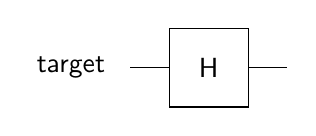
\begin{tikzpicture}[scale=.5] \node[draw=none] at (-3.5, 0) {target}; \draw (-2,0) -- (-1, 0); \draw (1, 0) -- (2, 0); \draw (-1,-1)--(-1,1)--(1,1)--(1,-1)--cycle; \node[draw=none] at (0, 0) {H}; \end{tikzpicture} } \] ~\newline
 
\begin{DoxyParams}[1]{Parameters}
\mbox{\tt in,out}  & {\em multi\+Qubit} & object representing the set of all qubits \\
\hline
\mbox{\tt in}  & {\em target\+Qubit} & qubit to operate on \\
\hline
\end{DoxyParams}

\begin{DoxyExceptions}{Exceptions}
{\em exit\+With\+Error} & if {\ttfamily target\+Qubit} is outside \mbox{[}0, {\ttfamily multi\+Qubit.\+num\+Qubits}). \\
\hline
\end{DoxyExceptions}


Definition at line 169 of file Qu\+E\+S\+T\+\_\+env\+\_\+local.\+c.



References Multi\+Qubit\+::chunk\+Id, chunk\+Is\+Upper(), exchange\+State\+Vectors(), get\+Chunk\+Pair\+Id(), hadamard\+Distributed(), hadamard\+Local(), half\+Matrix\+Block\+Fits\+In\+Chunk(), Multi\+Qubit\+::num\+Amps\+Per\+Chunk, Multi\+Qubit\+::num\+Qubits, Multi\+Qubit\+::pair\+State\+Vec, Qu\+E\+S\+T\+Assert(), R\+E\+AL, and Multi\+Qubit\+::state\+Vec.



Referenced by main(), and test\+\_\+hadamard().


\begin{DoxyCode}
170 \{
171     \mbox{\hyperlink{QuEST__env__local_8c_a3587b9d533e633ccf1abf9ad2ce45d8d}{QuESTAssert}}(targetQubit >= 0 && targetQubit < multiQubit.
      \mbox{\hyperlink{structMultiQubit_ab5b9795bdc6fb5855e1974dcbbaeb36f}{numQubits}}, 1, \_\_func\_\_);
172     \mbox{\hyperlink{QuEST_8c_aa9f0718b4dd794a3e1b143e3b153bfc5}{hadamardLocal}}(multiQubit, targetQubit);
173 \}
\end{DoxyCode}
\mbox{\Hypertarget{QuEST_8h_ae1b983b41249836ed2c2a81f77d83c40}\label{QuEST_8h_ae1b983b41249836ed2c2a81f77d83c40}} 
\index{Qu\+E\+S\+T.\+h@{Qu\+E\+S\+T.\+h}!init\+Classical\+State@{init\+Classical\+State}}
\index{init\+Classical\+State@{init\+Classical\+State}!Qu\+E\+S\+T.\+h@{Qu\+E\+S\+T.\+h}}
\paragraph{\texorpdfstring{init\+Classical\+State()}{initClassicalState()}}
{\footnotesize\ttfamily void init\+Classical\+State (\begin{DoxyParamCaption}\item[{\mbox{\hyperlink{structMultiQubit}{Multi\+Qubit}}}]{multi\+Qubit,  }\item[{long long int}]{state\+Ind }\end{DoxyParamCaption})}



Initialise a set of $ N $ qubits to the classical state with index {\ttfamily state\+Ind}. 

Note $ | 00 \dots 00 \rangle $ has {\ttfamily state\+Ind} 0, $ | 00 \dots 01 \rangle $ has {\ttfamily state\+Ind} 1, $ | 11 \dots 11 \rangle $ has {\ttfamily state\+Ind} $ 2^N - 1 $, etc. Subsequent calls to get\+Prob\+El will yield 0 for all indices except {\ttfamily state\+Ind}.


\begin{DoxyParams}[1]{Parameters}
\mbox{\tt in,out}  & {\em multi\+Qubit} & the object representing the set of qubits to be initialised \\
\hline
\mbox{\tt in}  & {\em state\+Ind} & the index (0 to the number of amplitudes, exclusive) of the state to give probability 1 \\
\hline
\end{DoxyParams}


Definition at line 222 of file Qu\+E\+S\+T.\+c.



References Multi\+Qubit\+::chunk\+Id, Multi\+Qubit\+::device\+State\+Vec, Complex\+Array\+::imag, Multi\+Qubit\+::num\+Amps\+Per\+Chunk, Complex\+Array\+::real, R\+E\+AL, and Multi\+Qubit\+::state\+Vec.



Referenced by test\+\_\+init\+Classical\+State().


\begin{DoxyCode}
223 \{
224     \textcolor{keywordtype}{long} \textcolor{keywordtype}{long} \textcolor{keywordtype}{int} stateVecSize;
225     \textcolor{keywordtype}{long} \textcolor{keywordtype}{long} \textcolor{keywordtype}{int} index;
226 
227     \textcolor{comment}{// dimension of the state vector}
228     stateVecSize = multiQubit.\mbox{\hyperlink{structMultiQubit_a1cad83601a78635dd278259c7ed54f18}{numAmpsPerChunk}};
229 
230     \textcolor{comment}{// Can't use multiQubit->stateVec as a private OMP var}
231     \mbox{\hyperlink{QuEST__precision_8h_a4b654506f18b8bfd61ad2a29a7e38c25}{REAL}} *stateVecReal = multiQubit.\mbox{\hyperlink{structMultiQubit_a45483190d6b01ef6b2f98f2bec9ab94f}{stateVec}}.\mbox{\hyperlink{structComplexArray_a4195cac6c784ea1b6271f1c7dba1548a}{real}};
232     \mbox{\hyperlink{QuEST__precision_8h_a4b654506f18b8bfd61ad2a29a7e38c25}{REAL}} *stateVecImag = multiQubit.\mbox{\hyperlink{structMultiQubit_a45483190d6b01ef6b2f98f2bec9ab94f}{stateVec}}.\mbox{\hyperlink{structComplexArray_a79dde47c7ae530c79cebfdf57b225968}{imag}};
233 
234     \textcolor{comment}{// initialise the state to |0000..0000>}
235 \textcolor{preprocessor}{# ifdef \_OPENMP}
236 \textcolor{preprocessor}{# pragma omp parallel \(\backslash\)}
237 \textcolor{preprocessor}{    default  (none) \(\backslash\)}
238 \textcolor{preprocessor}{    shared   (stateInd, stateVecSize, stateVecReal, stateVecImag) \(\backslash\)}
239 \textcolor{preprocessor}{    private  (index) }
240 \textcolor{preprocessor}{# endif}
241     \{
242 \textcolor{preprocessor}{# ifdef \_OPENMP}
243 \textcolor{preprocessor}{# pragma omp for schedule (static)}
244 \textcolor{preprocessor}{# endif}
245         \textcolor{keywordflow}{for} (index=0; index<stateVecSize; index++) \{
246             stateVecReal[index] = 0.0;
247             stateVecImag[index] = 0.0;
248         \}
249     \}
250 
251         \textcolor{comment}{// give the specified classical state prob 1}
252     \textcolor{keywordflow}{if} (multiQubit.\mbox{\hyperlink{structMultiQubit_ab10c88249fa3825d6227ceec01d37e37}{chunkId}} == stateInd/stateVecSize)\{
253         stateVecReal[stateInd % stateVecSize] = 1.0;
254         stateVecImag[stateInd % stateVecSize] = 0.0;
255     \}
256 \}
\end{DoxyCode}
\mbox{\Hypertarget{QuEST_8h_ad84a3ce68d1ca02b4e3f741ea45b6054}\label{QuEST_8h_ad84a3ce68d1ca02b4e3f741ea45b6054}} 
\index{Qu\+E\+S\+T.\+h@{Qu\+E\+S\+T.\+h}!init\+Qu\+E\+S\+T\+Env@{init\+Qu\+E\+S\+T\+Env}}
\index{init\+Qu\+E\+S\+T\+Env@{init\+Qu\+E\+S\+T\+Env}!Qu\+E\+S\+T.\+h@{Qu\+E\+S\+T.\+h}}
\paragraph{\texorpdfstring{init\+Qu\+E\+S\+T\+Env()}{initQuESTEnv()}}
{\footnotesize\ttfamily void init\+Qu\+E\+S\+T\+Env (\begin{DoxyParamCaption}\item[{\mbox{\hyperlink{structQuESTEnv}{Qu\+E\+S\+T\+Env}} $\ast$}]{env }\end{DoxyParamCaption})}



Initialize the Qu\+E\+ST environment. 

If something needs to be done to set up the execution environment, such as initializing M\+PI when running in distributed mode, it is handled here


\begin{DoxyParams}[1]{Parameters}
\mbox{\tt in,out}  & {\em env} & object representing the execution environment. A single instance is used for each program \\
\hline
\end{DoxyParams}


Definition at line 23 of file Qu\+E\+S\+T\+\_\+env\+\_\+local.\+c.



References env, G\+P\+U\+Exists(), Qu\+E\+S\+T\+Env\+::num\+Ranks, Qu\+E\+S\+T\+Env\+::rank, and seed\+Qu\+E\+S\+T\+Default().



Referenced by main().


\begin{DoxyCode}
23                                 \{
24     \textcolor{comment}{// init MPI environment}
25     \mbox{\hyperlink{runTests_8c_a5fd8ba97fcae3408ae6221dfc3cc1f93}{env}}->\mbox{\hyperlink{structQuESTEnv_aa648bb336cf8598467cb62db00b9cee8}{rank}}=0;
26     \mbox{\hyperlink{runTests_8c_a5fd8ba97fcae3408ae6221dfc3cc1f93}{env}}->\mbox{\hyperlink{structQuESTEnv_af22aacd7c9905accae28484785c193b4}{numRanks}}=1;
27         
28         \mbox{\hyperlink{QuEST_8c_ab0ab3ec70938712c26988a6aa51263a0}{seedQuESTDefault}}();
29 \}
\end{DoxyCode}
\mbox{\Hypertarget{QuEST_8h_af8a0082e2f695145bbfbb572e4c2e4f1}\label{QuEST_8h_af8a0082e2f695145bbfbb572e4c2e4f1}} 
\index{Qu\+E\+S\+T.\+h@{Qu\+E\+S\+T.\+h}!init\+State\+Plus@{init\+State\+Plus}}
\index{init\+State\+Plus@{init\+State\+Plus}!Qu\+E\+S\+T.\+h@{Qu\+E\+S\+T.\+h}}
\paragraph{\texorpdfstring{init\+State\+Plus()}{initStatePlus()}}
{\footnotesize\ttfamily void init\+State\+Plus (\begin{DoxyParamCaption}\item[{\mbox{\hyperlink{structMultiQubit}{Multi\+Qubit}}}]{multi\+Qubit }\end{DoxyParamCaption})}



Initialise a set of $ N $ qubits to the plus state $ {| + \rangle}^{\otimes N} = \frac{1}{\sqrt{2^N}} (| 0 \rangle + | 1 \rangle)^{\otimes N} $. 

This is the product state of $N$ qubits where every classical state is uniformly populated with real coefficient $\frac{1}{\sqrt{2^N}}$. This is equivalent to applying a Hadamard to every qubit in the zero state\+: $ \hat{H}^{\otimes N} {|0\rangle}^{\otimes N} $


\begin{DoxyParams}[1]{Parameters}
\mbox{\tt in,out}  & {\em multi\+Qubit} & the object representing the set of qubits to be initialised \\
\hline
\end{DoxyParams}


Definition at line 189 of file Qu\+E\+S\+T.\+c.



References Multi\+Qubit\+::device\+State\+Vec, Complex\+Array\+::imag, Multi\+Qubit\+::num\+Amps\+Per\+Chunk, Multi\+Qubit\+::num\+Chunks, Complex\+Array\+::real, R\+E\+AL, and Multi\+Qubit\+::state\+Vec.



Referenced by test\+\_\+collapse\+To\+Outcome(), test\+\_\+compact\+Unitary(), test\+\_\+find\+Probability\+Of\+Outcome(), test\+\_\+init\+State\+Plus(), test\+\_\+measure(), test\+\_\+measure\+With\+Stats(), and test\+\_\+unitary().


\begin{DoxyCode}
190 \{
191     \textcolor{keywordtype}{long} \textcolor{keywordtype}{long} \textcolor{keywordtype}{int} chunkSize, stateVecSize;
192     \textcolor{keywordtype}{long} \textcolor{keywordtype}{long} \textcolor{keywordtype}{int} index;
193 
194     \textcolor{comment}{// dimension of the state vector}
195     chunkSize = multiQubit.\mbox{\hyperlink{structMultiQubit_a1cad83601a78635dd278259c7ed54f18}{numAmpsPerChunk}};
196     stateVecSize = chunkSize*multiQubit.\mbox{\hyperlink{structMultiQubit_acd43f2f57991709c9e94f73662c972b2}{numChunks}};
197     \mbox{\hyperlink{QuEST__precision_8h_a4b654506f18b8bfd61ad2a29a7e38c25}{REAL}} normFactor = 1.0/sqrt((\mbox{\hyperlink{QuEST__precision_8h_a4b654506f18b8bfd61ad2a29a7e38c25}{REAL}})stateVecSize);
198 
199     \textcolor{comment}{// Can't use multiQubit->stateVec as a private OMP var}
200     \mbox{\hyperlink{QuEST__precision_8h_a4b654506f18b8bfd61ad2a29a7e38c25}{REAL}} *stateVecReal = multiQubit.\mbox{\hyperlink{structMultiQubit_a45483190d6b01ef6b2f98f2bec9ab94f}{stateVec}}.\mbox{\hyperlink{structComplexArray_a4195cac6c784ea1b6271f1c7dba1548a}{real}};
201     \mbox{\hyperlink{QuEST__precision_8h_a4b654506f18b8bfd61ad2a29a7e38c25}{REAL}} *stateVecImag = multiQubit.\mbox{\hyperlink{structMultiQubit_a45483190d6b01ef6b2f98f2bec9ab94f}{stateVec}}.\mbox{\hyperlink{structComplexArray_a79dde47c7ae530c79cebfdf57b225968}{imag}};
202 
203     \textcolor{comment}{// initialise the state to |0000..0000>}
204 \textcolor{preprocessor}{# ifdef \_OPENMP}
205 \textcolor{preprocessor}{# pragma omp parallel \(\backslash\)}
206 \textcolor{preprocessor}{    default  (none) \(\backslash\)}
207 \textcolor{preprocessor}{    shared   (chunkSize, stateVecReal, stateVecImag, normFactor) \(\backslash\)}
208 \textcolor{preprocessor}{    private  (index) }
209 \textcolor{preprocessor}{# endif}
210     \{
211 \textcolor{preprocessor}{# ifdef \_OPENMP}
212 \textcolor{preprocessor}{# pragma omp for schedule (static)}
213 \textcolor{preprocessor}{# endif}
214         \textcolor{keywordflow}{for} (index=0; index<chunkSize; index++) \{
215             stateVecReal[index] = normFactor;
216             stateVecImag[index] = 0.0;
217         \}
218     \}
219 \}
\end{DoxyCode}
\mbox{\Hypertarget{QuEST_8h_a9ba8171c9ec5c42202b144026527e9ec}\label{QuEST_8h_a9ba8171c9ec5c42202b144026527e9ec}} 
\index{Qu\+E\+S\+T.\+h@{Qu\+E\+S\+T.\+h}!init\+State\+Zero@{init\+State\+Zero}}
\index{init\+State\+Zero@{init\+State\+Zero}!Qu\+E\+S\+T.\+h@{Qu\+E\+S\+T.\+h}}
\paragraph{\texorpdfstring{init\+State\+Zero()}{initStateZero()}}
{\footnotesize\ttfamily void init\+State\+Zero (\begin{DoxyParamCaption}\item[{\mbox{\hyperlink{structMultiQubit}{Multi\+Qubit}}}]{multi\+Qubit }\end{DoxyParamCaption})}



Initialise a set of $ N $ qubits to the classical zero state $ {| 0 \rangle}^{\otimes N} $. 


\begin{DoxyParams}[1]{Parameters}
\mbox{\tt in,out}  & {\em multi\+Qubit} & the object representing the set of all qubits to initialise \\
\hline
\end{DoxyParams}


Definition at line 153 of file Qu\+E\+S\+T.\+c.



References Multi\+Qubit\+::chunk\+Id, Multi\+Qubit\+::device\+State\+Vec, Complex\+Array\+::imag, Multi\+Qubit\+::num\+Amps\+Per\+Chunk, Complex\+Array\+::real, R\+E\+AL, and Multi\+Qubit\+::state\+Vec.



Referenced by main(), test\+\_\+collapse\+To\+Outcome(), test\+\_\+find\+Probability\+Of\+Outcome(), test\+\_\+init\+State\+Zero(), test\+\_\+measure(), and test\+\_\+measure\+With\+Stats().


\begin{DoxyCode}
154 \{
155     \textcolor{keywordtype}{long} \textcolor{keywordtype}{long} \textcolor{keywordtype}{int} stateVecSize;
156     \textcolor{keywordtype}{long} \textcolor{keywordtype}{long} \textcolor{keywordtype}{int} index;
157 
158     \textcolor{comment}{// dimension of the state vector}
159     stateVecSize = multiQubit.\mbox{\hyperlink{structMultiQubit_a1cad83601a78635dd278259c7ed54f18}{numAmpsPerChunk}};
160 
161     \textcolor{comment}{// Can't use multiQubit->stateVec as a private OMP var}
162     \mbox{\hyperlink{QuEST__precision_8h_a4b654506f18b8bfd61ad2a29a7e38c25}{REAL}} *stateVecReal = multiQubit.\mbox{\hyperlink{structMultiQubit_a45483190d6b01ef6b2f98f2bec9ab94f}{stateVec}}.\mbox{\hyperlink{structComplexArray_a4195cac6c784ea1b6271f1c7dba1548a}{real}};
163     \mbox{\hyperlink{QuEST__precision_8h_a4b654506f18b8bfd61ad2a29a7e38c25}{REAL}} *stateVecImag = multiQubit.\mbox{\hyperlink{structMultiQubit_a45483190d6b01ef6b2f98f2bec9ab94f}{stateVec}}.\mbox{\hyperlink{structComplexArray_a79dde47c7ae530c79cebfdf57b225968}{imag}};
164 
165     \textcolor{comment}{// initialise the state to |0000..0000>}
166 \textcolor{preprocessor}{# ifdef \_OPENMP}
167 \textcolor{preprocessor}{# pragma omp parallel \(\backslash\)}
168 \textcolor{preprocessor}{    default  (none) \(\backslash\)}
169 \textcolor{preprocessor}{    shared   (stateVecSize, stateVecReal, stateVecImag) \(\backslash\)}
170 \textcolor{preprocessor}{    private  (index) }
171 \textcolor{preprocessor}{# endif}
172     \{
173 \textcolor{preprocessor}{# ifdef \_OPENMP}
174 \textcolor{preprocessor}{# pragma omp for schedule (static)}
175 \textcolor{preprocessor}{# endif}
176         \textcolor{keywordflow}{for} (index=0; index<stateVecSize; index++) \{
177             stateVecReal[index] = 0.0;
178             stateVecImag[index] = 0.0;
179         \}
180     \}
181 
182     \textcolor{keywordflow}{if} (multiQubit.\mbox{\hyperlink{structMultiQubit_ab10c88249fa3825d6227ceec01d37e37}{chunkId}}==0)\{
183         \textcolor{comment}{// zero state |0000..0000> has probability 1}
184         stateVecReal[0] = 1.0;
185         stateVecImag[0] = 0.0;
186     \}
187 \}
\end{DoxyCode}
\mbox{\Hypertarget{QuEST_8h_ad5774247d836267175c664cd0e451bcb}\label{QuEST_8h_ad5774247d836267175c664cd0e451bcb}} 
\index{Qu\+E\+S\+T.\+h@{Qu\+E\+S\+T.\+h}!measure@{measure}}
\index{measure@{measure}!Qu\+E\+S\+T.\+h@{Qu\+E\+S\+T.\+h}}
\paragraph{\texorpdfstring{measure()}{measure()}}
{\footnotesize\ttfamily int measure (\begin{DoxyParamCaption}\item[{\mbox{\hyperlink{structMultiQubit}{Multi\+Qubit}}}]{multi\+Qubit,  }\item[{int}]{measure\+Qubit }\end{DoxyParamCaption})}



Measures a single qubit, collapsing it randomly to 0 or 1. 

Outcome probabilities are weighted by the state vector, which is irreversibly changed after collapse to be consistent with the outcome.


\begin{DoxyParams}[1]{Parameters}
\mbox{\tt in,out}  & {\em multi\+Qubit} & object representing the set of all qubits \\
\hline
\mbox{\tt in}  & {\em measure\+Qubit} & qubit to measure \\
\hline
\end{DoxyParams}
\begin{DoxyReturn}{Returns}
the measurement outcome, 0 or 1 
\end{DoxyReturn}

\begin{DoxyExceptions}{Exceptions}
{\em exit\+With\+Error} & if {\ttfamily measure\+Qubit} is outside \mbox{[}0, {\ttfamily multi\+Qubit.\+num\+Qubits}) \\
\hline
\end{DoxyExceptions}


Definition at line 203 of file Qu\+E\+S\+T\+\_\+env\+\_\+local.\+c.



References measure\+With\+Stats(), Multi\+Qubit\+::num\+Qubits, Qu\+E\+S\+T\+Assert(), and R\+E\+AL.



Referenced by main(), and test\+\_\+measure().


\begin{DoxyCode}
203                                                     \{
204     \mbox{\hyperlink{QuEST__env__local_8c_a3587b9d533e633ccf1abf9ad2ce45d8d}{QuESTAssert}}(measureQubit >= 0 && measureQubit < multiQubit.
      \mbox{\hyperlink{structMultiQubit_ab5b9795bdc6fb5855e1974dcbbaeb36f}{numQubits}}, 2, \_\_func\_\_);
205     \mbox{\hyperlink{QuEST__precision_8h_a4b654506f18b8bfd61ad2a29a7e38c25}{REAL}} stateProb;
206     \textcolor{keywordflow}{return} \mbox{\hyperlink{QuEST__env__local_8c_a2ac46e470c750bf93c754e06c64b0a7a}{measureWithStats}}(multiQubit, measureQubit, &stateProb);
207 \}
\end{DoxyCode}
\mbox{\Hypertarget{QuEST_8h_a2ac46e470c750bf93c754e06c64b0a7a}\label{QuEST_8h_a2ac46e470c750bf93c754e06c64b0a7a}} 
\index{Qu\+E\+S\+T.\+h@{Qu\+E\+S\+T.\+h}!measure\+With\+Stats@{measure\+With\+Stats}}
\index{measure\+With\+Stats@{measure\+With\+Stats}!Qu\+E\+S\+T.\+h@{Qu\+E\+S\+T.\+h}}
\paragraph{\texorpdfstring{measure\+With\+Stats()}{measureWithStats()}}
{\footnotesize\ttfamily int measure\+With\+Stats (\begin{DoxyParamCaption}\item[{\mbox{\hyperlink{structMultiQubit}{Multi\+Qubit}}}]{multi\+Qubit,  }\item[{int}]{measure\+Qubit,  }\item[{\mbox{\hyperlink{QuEST__precision_8h_a4b654506f18b8bfd61ad2a29a7e38c25}{R\+E\+AL}} $\ast$}]{state\+Prob }\end{DoxyParamCaption})}



Measures a single qubit, collapsing it randomly to 0 or 1, and additionally gives the probability of that outcome. 

Outcome probabilities are weighted by the state vector, which is irreversibly changed after collapse to be consistent with the outcome.


\begin{DoxyParams}[1]{Parameters}
\mbox{\tt in,out}  & {\em multi\+Qubit} & object representing the set of all qubits \\
\hline
\mbox{\tt in}  & {\em measure\+Qubit} & qubit to measure \\
\hline
\mbox{\tt out}  & {\em state\+Prob} & a pointer to a R\+E\+AL which is set to the probability of the occurred outcome \\
\hline
\end{DoxyParams}
\begin{DoxyReturn}{Returns}
the measurement outcome, 0 or 1 
\end{DoxyReturn}

\begin{DoxyExceptions}{Exceptions}
{\em exit\+With\+Error} & if {\ttfamily measure\+Qubit} is outside \mbox{[}0, {\ttfamily multi\+Qubit.\+num\+Qubits}) \\
\hline
\end{DoxyExceptions}


Definition at line 209 of file Qu\+E\+S\+T\+\_\+env\+\_\+local.\+c.



References Multi\+Qubit\+::chunk\+Id, collapse\+To\+Outcome\+Distributed\+Renorm(), collapse\+To\+Outcome\+Distributed\+Set\+Zero(), collapse\+To\+Outcome\+Local(), find\+Probability\+Of\+Outcome(), genrand\+\_\+real1(), half\+Matrix\+Block\+Fits\+In\+Chunk(), is\+Chunk\+To\+Skip\+In\+Find\+P\+Zero(), Multi\+Qubit\+::num\+Amps\+Per\+Chunk, Multi\+Qubit\+::num\+Qubits, Qu\+E\+S\+T\+Assert(), R\+E\+AL, and R\+E\+A\+L\+\_\+\+E\+PS.



Referenced by main(), measure(), and test\+\_\+measure\+With\+Stats().


\begin{DoxyCode}
209                                                                               \{
210     \mbox{\hyperlink{QuEST__env__local_8c_a3587b9d533e633ccf1abf9ad2ce45d8d}{QuESTAssert}}(measureQubit >= 0 && measureQubit < multiQubit.
      \mbox{\hyperlink{structMultiQubit_ab5b9795bdc6fb5855e1974dcbbaeb36f}{numQubits}}, 2, \_\_func\_\_);
211 
212     \textcolor{keywordtype}{int} outcome;
213     \textcolor{comment}{// find probability of qubit being in state 1}
214     \mbox{\hyperlink{QuEST__precision_8h_a4b654506f18b8bfd61ad2a29a7e38c25}{REAL}} stateProbInternal = \mbox{\hyperlink{QuEST__env__local_8c_ad315c941a51bc053d39ebfa2040fd32e}{findProbabilityOfOutcome}}(multiQubit, measureQubit,
       1);
215 
216     \textcolor{comment}{// we can't collapse to a state that has a probability too close to zero}
217     \textcolor{keywordflow}{if} (stateProbInternal<\mbox{\hyperlink{QuEST__precision_8h_aebb5e6716e06431296af4d1a71744dec}{REAL\_EPS}}) outcome=0;
218     \textcolor{keywordflow}{else} \textcolor{keywordflow}{if} (1-stateProbInternal<\mbox{\hyperlink{QuEST__precision_8h_aebb5e6716e06431296af4d1a71744dec}{REAL\_EPS}}) outcome=1;
219     \textcolor{keywordflow}{else} \{
220         \textcolor{comment}{// ok. both P(0) and P(1) are large enough to resolve}
221         \textcolor{comment}{// generate random float on [0,1]}
222         \textcolor{keywordtype}{float} randNum = \mbox{\hyperlink{mt19937ar_8c_ac94ab75771800274ed1a2bedeca86f04}{genrand\_real1}}();
223         \textcolor{keywordflow}{if} (randNum<=stateProbInternal) outcome = 1;
224         \textcolor{keywordflow}{else} outcome = 0;
225     \} 
226     \textcolor{keywordflow}{if} (outcome==0) stateProbInternal = 1-stateProbInternal;
227     \mbox{\hyperlink{QuEST_8c_a01d9a8b7ff0e09ec399e158389783aa9}{collapseToOutcomeLocal}}(multiQubit, measureQubit, stateProbInternal, outcome);
228     *stateProb = stateProbInternal;
229     \textcolor{keywordflow}{return} outcome;
230 \}
\end{DoxyCode}
\mbox{\Hypertarget{QuEST_8h_afc1835c6b43b6e59ce7df7b13f274fc7}\label{QuEST_8h_afc1835c6b43b6e59ce7df7b13f274fc7}} 
\index{Qu\+E\+S\+T.\+h@{Qu\+E\+S\+T.\+h}!multi\+Controlled\+Phase\+Gate@{multi\+Controlled\+Phase\+Gate}}
\index{multi\+Controlled\+Phase\+Gate@{multi\+Controlled\+Phase\+Gate}!Qu\+E\+S\+T.\+h@{Qu\+E\+S\+T.\+h}}
\paragraph{\texorpdfstring{multi\+Controlled\+Phase\+Gate()}{multiControlledPhaseGate()}}
{\footnotesize\ttfamily void multi\+Controlled\+Phase\+Gate (\begin{DoxyParamCaption}\item[{\mbox{\hyperlink{structMultiQubit}{Multi\+Qubit}}}]{multi\+Qubit,  }\item[{int $\ast$}]{control\+Qubits,  }\item[{int}]{num\+Control\+Qubits }\end{DoxyParamCaption})}



Apply the multiple-\/qubit controlled phase gate, also known as the multiple-\/qubit controlled sigmaZ gate. 

For each state, if all control qubits have value one, multiply the amplitude of that state by -\/1. This applies the many-\/qubit unitary\+: \[ \begin{pmatrix} 1 \\ & 1 \\\ & & \ddots \\ & & & 1 \\ & & & & -1 \end{pmatrix} \] on the control qubits.

\[ \setlength{\fboxrule}{0.01pt} \fbox{ \begin{tikzpicture}[scale=.5] \node[draw=none] at (-3.5, 2) {controls}; \node[draw=none] at (0, 6) {$\vdots$}; \draw (0, 5) -- (0, 4); \draw (-2, 4) -- (2, 4); \draw[fill=black] (0, 4) circle (.2); \draw (0, 4) -- (0, 2); \draw (-2, 2) -- (2, 2); \draw[fill=black] (0, 2) circle (.2); \draw (0, 2) -- (0, 0); \draw (-2,0) -- (2, 0); \draw[fill=black] (0, 0) circle (.2); \end{tikzpicture} } \]


\begin{DoxyParams}[1]{Parameters}
\mbox{\tt in,out}  & {\em multi\+Qubit} & object representing the set of all qubits \\
\hline
\mbox{\tt in}  & {\em control\+Qubits} & array of input qubits \\
\hline
\mbox{\tt in}  & {\em num\+Control\+Qubits} & number of input qubits \\
\hline
\end{DoxyParams}

\begin{DoxyExceptions}{Exceptions}
{\em exit\+With\+Error} & if {\ttfamily num\+Control\+Qubits} is outside \mbox{[}1, {\ttfamily multi\+Qubit.\+num\+Qubits}) \\
\hline
\end{DoxyExceptions}


Definition at line 1783 of file Qu\+E\+S\+T.\+c.



References Multi\+Qubit\+::chunk\+Id, Complex\+Array\+::imag, Multi\+Qubit\+::num\+Amps\+Per\+Chunk, Multi\+Qubit\+::num\+Qubits, Qu\+E\+S\+T\+Assert(), Complex\+Array\+::real, R\+E\+AL, and Multi\+Qubit\+::state\+Vec.



Referenced by main(), and test\+\_\+multi\+Controlled\+Phase\+Gate().


\begin{DoxyCode}
1784 \{
1785     \textcolor{keywordtype}{long} \textcolor{keywordtype}{long} \textcolor{keywordtype}{int} index;
1786     \textcolor{keywordtype}{long} \textcolor{keywordtype}{long} \textcolor{keywordtype}{int} stateVecSize;
1787 
1788     \textcolor{keyword}{const} \textcolor{keywordtype}{long} \textcolor{keywordtype}{long} \textcolor{keywordtype}{int} chunkSize=multiQubit.\mbox{\hyperlink{structMultiQubit_a1cad83601a78635dd278259c7ed54f18}{numAmpsPerChunk}};
1789     \textcolor{keyword}{const} \textcolor{keywordtype}{long} \textcolor{keywordtype}{long} \textcolor{keywordtype}{int} chunkId=multiQubit.\mbox{\hyperlink{structMultiQubit_ab10c88249fa3825d6227ceec01d37e37}{chunkId}};
1790 
1791     \mbox{\hyperlink{QuEST__env__local_8c_a3587b9d533e633ccf1abf9ad2ce45d8d}{QuESTAssert}}(numControlQubits > 0 && numControlQubits <= multiQubit.
      \mbox{\hyperlink{structMultiQubit_ab5b9795bdc6fb5855e1974dcbbaeb36f}{numQubits}}, 4, \_\_func\_\_);
1792     \textcolor{keywordtype}{long} \textcolor{keywordtype}{long} \textcolor{keywordtype}{int} mask=0;
1793     \textcolor{keywordflow}{for} (\textcolor{keywordtype}{int} i=0; i<numControlQubits; i++) mask = mask | (1LL<<controlQubits[i]);
1794     \mbox{\hyperlink{QuEST__env__local_8c_a3587b9d533e633ccf1abf9ad2ce45d8d}{QuESTAssert}}(mask >=0 && mask <= (1LL<<multiQubit.\mbox{\hyperlink{structMultiQubit_ab5b9795bdc6fb5855e1974dcbbaeb36f}{numQubits}})-1, 2, \_\_func\_\_);
1795 
1796     stateVecSize = multiQubit.\mbox{\hyperlink{structMultiQubit_a1cad83601a78635dd278259c7ed54f18}{numAmpsPerChunk}};
1797     \mbox{\hyperlink{QuEST__precision_8h_a4b654506f18b8bfd61ad2a29a7e38c25}{REAL}} *stateVecReal = multiQubit.\mbox{\hyperlink{structMultiQubit_a45483190d6b01ef6b2f98f2bec9ab94f}{stateVec}}.\mbox{\hyperlink{structComplexArray_a4195cac6c784ea1b6271f1c7dba1548a}{real}};
1798     \mbox{\hyperlink{QuEST__precision_8h_a4b654506f18b8bfd61ad2a29a7e38c25}{REAL}} *stateVecImag = multiQubit.\mbox{\hyperlink{structMultiQubit_a45483190d6b01ef6b2f98f2bec9ab94f}{stateVec}}.\mbox{\hyperlink{structComplexArray_a79dde47c7ae530c79cebfdf57b225968}{imag}};
1799 
1800 \textcolor{preprocessor}{# ifdef \_OPENMP}
1801 \textcolor{preprocessor}{# pragma omp parallel \(\backslash\)}
1802 \textcolor{preprocessor}{    default  (none)                          \(\backslash\)}
1803 \textcolor{preprocessor}{    shared   (stateVecSize, stateVecReal,stateVecImag, mask ) \(\backslash\)}
1804 \textcolor{preprocessor}{    private  (index)}
1805 \textcolor{preprocessor}{# endif}
1806     \{
1807 \textcolor{preprocessor}{# ifdef \_OPENMP}
1808 \textcolor{preprocessor}{# pragma omp for schedule (static)}
1809 \textcolor{preprocessor}{# endif}
1810         \textcolor{keywordflow}{for} (index=0; index<stateVecSize; index++) \{
1811             \textcolor{keywordflow}{if} (mask == (mask & (index+chunkId*chunkSize)) )\{
1812                 stateVecReal [index] = - stateVecReal [index];
1813                 stateVecImag [index] = - stateVecImag [index];
1814             \}
1815         \}
1816     \}
1817 \}
\end{DoxyCode}
\mbox{\Hypertarget{QuEST_8h_ae395a79690283ed81106afadd7a8cd8a}\label{QuEST_8h_ae395a79690283ed81106afadd7a8cd8a}} 
\index{Qu\+E\+S\+T.\+h@{Qu\+E\+S\+T.\+h}!multi\+Controlled\+Unitary@{multi\+Controlled\+Unitary}}
\index{multi\+Controlled\+Unitary@{multi\+Controlled\+Unitary}!Qu\+E\+S\+T.\+h@{Qu\+E\+S\+T.\+h}}
\paragraph{\texorpdfstring{multi\+Controlled\+Unitary()}{multiControlledUnitary()}}
{\footnotesize\ttfamily void multi\+Controlled\+Unitary (\begin{DoxyParamCaption}\item[{\mbox{\hyperlink{structMultiQubit}{Multi\+Qubit}}}]{multi\+Qubit,  }\item[{int $\ast$}]{control\+Qubits,  }\item[{const int}]{num\+Control\+Qubits,  }\item[{const int}]{target\+Qubit,  }\item[{\mbox{\hyperlink{structComplexMatrix2}{Complex\+Matrix2}}}]{u }\end{DoxyParamCaption})}



Apply a general multiple-\/control single-\/target unitary, which can include a global phase factor. 

Any number of control qubits can be specified, and if all have value 1, the given unitary is applied to the target qubit. This effects the many-\/qubit unitary \[ \begin{pmatrix} 1 \\ & 1 \\\ & & \ddots \\ & & & u_{00} & u_{01}\\ & & & u_{10} & u_{11} \end{pmatrix} \] on the control and target qubits. The given 2x2 Complex\+Matrix must be unitary, otherwise an error is thrown.

\[ \setlength{\fboxrule}{0.01pt} \fbox{ 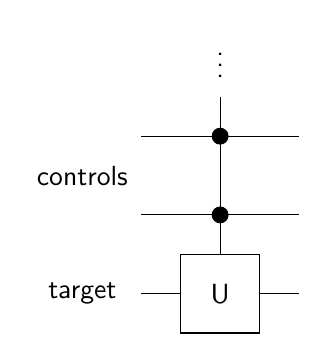
\begin{tikzpicture}[scale=.5] \node[draw=none] at (-3.5, 3) {controls}; \node[draw=none] at (-3.5, 0) {target}; \node[draw=none] at (0, 6) {$\vdots$}; \draw (0, 5) -- (0, 4); \draw (-2, 4) -- (2, 4); \draw[fill=black] (0, 4) circle (.2); \draw (0, 4) -- (0, 2); \draw (-2, 2) -- (2, 2); \draw[fill=black] (0, 2) circle (.2); \draw (0, 2) -- (0, 1); \draw (-2,0) -- (-1, 0); \draw (1, 0) -- (2, 0); \draw (-1,-1)--(-1,1)--(1,1)--(1,-1)--cycle; \node[draw=none] at (0, 0) {U}; \end{tikzpicture} } \]


\begin{DoxyParams}[1]{Parameters}
\mbox{\tt in,out}  & {\em multi\+Qubit} & object representing the set of all qubits \\
\hline
\mbox{\tt in}  & {\em control\+Qubits} & applies unitary if all qubits in this array equal 1 \\
\hline
\mbox{\tt in}  & {\em num\+Control\+Qubits} & number of control qubits \\
\hline
\mbox{\tt in}  & {\em target\+Qubit} & qubit to operate on \\
\hline
\mbox{\tt in}  & {\em u} & single-\/qubit unitary matrix to apply \\
\hline
\end{DoxyParams}

\begin{DoxyExceptions}{Exceptions}
{\em exit\+With\+Error} & if {\ttfamily num\+Control\+Qubits} is outside \mbox{[}1, {\ttfamily multi\+Qubit.\+num\+Qubits}\mbox{]}), or if any qubit index ({\ttfamily target\+Qubit} or one in {\ttfamily control\+Qubits}) is outside \mbox{[}0, {\ttfamily multi\+Qubit.\+num\+Qubits}\mbox{]}), or if {\ttfamily control\+Qubits} contains {\ttfamily target\+Qubit}, or if {\ttfamily u} is not unitary. \\
\hline
\end{DoxyExceptions}


Definition at line 137 of file Qu\+E\+S\+T\+\_\+env\+\_\+local.\+c.



References Multi\+Qubit\+::chunk\+Id, chunk\+Is\+Upper(), exchange\+State\+Vectors(), get\+Chunk\+Pair\+Id(), get\+Rot\+Angle\+From\+Unitary\+Matrix(), half\+Matrix\+Block\+Fits\+In\+Chunk(), multi\+Controlled\+Unitary\+Distributed(), multi\+Controlled\+Unitary\+Local(), Multi\+Qubit\+::num\+Amps\+Per\+Chunk, Multi\+Qubit\+::num\+Qubits, Multi\+Qubit\+::pair\+State\+Vec, Qu\+E\+S\+T\+Assert(), R\+E\+AL, Multi\+Qubit\+::state\+Vec, and validate\+Matrix\+Is\+Unitary().



Referenced by main(), and test\+\_\+multi\+Controlled\+Unitary().


\begin{DoxyCode}
138 \{
139     \mbox{\hyperlink{QuEST__env__local_8c_a3587b9d533e633ccf1abf9ad2ce45d8d}{QuESTAssert}}(targetQubit >= 0 && targetQubit < multiQubit.
      \mbox{\hyperlink{structMultiQubit_ab5b9795bdc6fb5855e1974dcbbaeb36f}{numQubits}}, 1, \_\_func\_\_);
140     \mbox{\hyperlink{QuEST__env__local_8c_a3587b9d533e633ccf1abf9ad2ce45d8d}{QuESTAssert}}(numControlQubits > 0 && numControlQubits <= multiQubit.
      \mbox{\hyperlink{structMultiQubit_ab5b9795bdc6fb5855e1974dcbbaeb36f}{numQubits}}, 4, \_\_func\_\_);
141     \mbox{\hyperlink{QuEST__env__local_8c_a3587b9d533e633ccf1abf9ad2ce45d8d}{QuESTAssert}}(\mbox{\hyperlink{QuEST_8c_ae4fea133d1a8f09ff8da03038100adb2}{validateMatrixIsUnitary}}(u), 5, \_\_func\_\_);
142 
143     \textcolor{keywordtype}{long} \textcolor{keywordtype}{long} \textcolor{keywordtype}{int} mask=0; 
144     \textcolor{keywordflow}{for} (\textcolor{keywordtype}{int} i=0; i<numControlQubits; i++) mask = mask | (1LL<<controlQubits[i]);
145     \mbox{\hyperlink{QuEST__env__local_8c_a3587b9d533e633ccf1abf9ad2ce45d8d}{QuESTAssert}}(mask >=0 && mask <= (1LL<<multiQubit.\mbox{\hyperlink{structMultiQubit_ab5b9795bdc6fb5855e1974dcbbaeb36f}{numQubits}})-1, 2, \_\_func\_\_);
146     \mbox{\hyperlink{QuEST__env__local_8c_a3587b9d533e633ccf1abf9ad2ce45d8d}{QuESTAssert}}((mask & (1LL<<targetQubit)) != (1LL<<targetQubit), 3, \_\_func\_\_);
147 
148     \mbox{\hyperlink{QuEST_8c_a1309eabcba3cb97fbc3cd2e606d17766}{multiControlledUnitaryLocal}}(multiQubit, targetQubit, mask, u);
149 \}
\end{DoxyCode}
\mbox{\Hypertarget{QuEST_8h_aa5e77e0e64f3a4a3d3f5cc7382bffcd9}\label{QuEST_8h_aa5e77e0e64f3a4a3d3f5cc7382bffcd9}} 
\index{Qu\+E\+S\+T.\+h@{Qu\+E\+S\+T.\+h}!report\+Multi\+Qubit\+Params@{report\+Multi\+Qubit\+Params}}
\index{report\+Multi\+Qubit\+Params@{report\+Multi\+Qubit\+Params}!Qu\+E\+S\+T.\+h@{Qu\+E\+S\+T.\+h}}
\paragraph{\texorpdfstring{report\+Multi\+Qubit\+Params()}{reportMultiQubitParams()}}
{\footnotesize\ttfamily void report\+Multi\+Qubit\+Params (\begin{DoxyParamCaption}\item[{\mbox{\hyperlink{structMultiQubit}{Multi\+Qubit}}}]{multi\+Qubit }\end{DoxyParamCaption})}



Report metainformation about a set of qubits\+: number of qubits, number of probability amplitudes. 


\begin{DoxyParams}[1]{Parameters}
\mbox{\tt in,out}  & {\em multi\+Qubit} & object representing the set of qubits \\
\hline
\mbox{\tt in}  & {\em env} & object representing the execution environment (local, multinode etc) \\
\hline
\end{DoxyParams}


Definition at line 125 of file Qu\+E\+S\+T.\+c.



References Multi\+Qubit\+::chunk\+Id, Multi\+Qubit\+::num\+Chunks, and Multi\+Qubit\+::num\+Qubits.



Referenced by main().


\begin{DoxyCode}
125                                                   \{
126     \textcolor{keywordtype}{long} \textcolor{keywordtype}{long} \textcolor{keywordtype}{int} numAmps = 1L << multiQubit.\mbox{\hyperlink{structMultiQubit_ab5b9795bdc6fb5855e1974dcbbaeb36f}{numQubits}};
127     \textcolor{keywordtype}{long} \textcolor{keywordtype}{long} \textcolor{keywordtype}{int} numAmpsPerRank = numAmps/multiQubit.\mbox{\hyperlink{structMultiQubit_acd43f2f57991709c9e94f73662c972b2}{numChunks}};
128     \textcolor{keywordflow}{if} (multiQubit.\mbox{\hyperlink{structMultiQubit_ab10c88249fa3825d6227ceec01d37e37}{chunkId}}==0)\{
129         printf(\textcolor{stringliteral}{"QUBITS:\(\backslash\)n"});
130         printf(\textcolor{stringliteral}{"Number of qubits is %d.\(\backslash\)n"}, multiQubit.\mbox{\hyperlink{structMultiQubit_ab5b9795bdc6fb5855e1974dcbbaeb36f}{numQubits}});
131         printf(\textcolor{stringliteral}{"Number of amps is %lld.\(\backslash\)n"}, numAmps);
132         printf(\textcolor{stringliteral}{"Number of amps per rank is %lld.\(\backslash\)n"}, numAmpsPerRank);
133     \}
134 \}
\end{DoxyCode}
\mbox{\Hypertarget{QuEST_8h_af8a14ae79c3fb2c0b5f6255cc37bebf9}\label{QuEST_8h_af8a14ae79c3fb2c0b5f6255cc37bebf9}} 
\index{Qu\+E\+S\+T.\+h@{Qu\+E\+S\+T.\+h}!report\+Qu\+E\+S\+T\+Env@{report\+Qu\+E\+S\+T\+Env}}
\index{report\+Qu\+E\+S\+T\+Env@{report\+Qu\+E\+S\+T\+Env}!Qu\+E\+S\+T.\+h@{Qu\+E\+S\+T.\+h}}
\paragraph{\texorpdfstring{report\+Qu\+E\+S\+T\+Env()}{reportQuESTEnv()}}
{\footnotesize\ttfamily void report\+Qu\+E\+S\+T\+Env (\begin{DoxyParamCaption}\item[{\mbox{\hyperlink{structQuESTEnv}{Qu\+E\+S\+T\+Env}}}]{env }\end{DoxyParamCaption})}



Report information about the Qu\+E\+ST environment. 


\begin{DoxyParams}[1]{Parameters}
\mbox{\tt in}  & {\em env} & object representing the execution environment. A single instance is used for each program \\
\hline
\end{DoxyParams}


Definition at line 43 of file Qu\+E\+S\+T\+\_\+env\+\_\+local.\+c.



References env, Qu\+E\+S\+T\+Env\+::num\+Ranks, Qu\+E\+S\+T\+Env\+::rank, and R\+E\+AL.



Referenced by main().


\begin{DoxyCode}
43                                  \{
44     printf(\textcolor{stringliteral}{"EXECUTION ENVIRONMENT:\(\backslash\)n"});
45     printf(\textcolor{stringliteral}{"Running locally on one node\(\backslash\)n"});
46     printf(\textcolor{stringliteral}{"Number of ranks is %d\(\backslash\)n"}, \mbox{\hyperlink{runTests_8c_a5fd8ba97fcae3408ae6221dfc3cc1f93}{env}}.\mbox{\hyperlink{structQuESTEnv_af22aacd7c9905accae28484785c193b4}{numRanks}});
47 \textcolor{preprocessor}{# ifdef \_OPENMP}
48     printf(\textcolor{stringliteral}{"OpenMP enabled\(\backslash\)n"});
49     printf(\textcolor{stringliteral}{"Number of threads available is %d\(\backslash\)n"}, omp\_get\_max\_threads());
50 \textcolor{preprocessor}{# else}
51     printf(\textcolor{stringliteral}{"OpenMP disabled\(\backslash\)n"});
52 \textcolor{preprocessor}{# endif}
53     printf(\textcolor{stringliteral}{"Precision: size of REAL is %ld bytes\(\backslash\)n"}, \textcolor{keyword}{sizeof}(\mbox{\hyperlink{QuEST__precision_8h_a4b654506f18b8bfd61ad2a29a7e38c25}{REAL}}));
54 \}
\end{DoxyCode}
\mbox{\Hypertarget{QuEST_8h_a96f4de9ce7fefc7680a44d601fc3d894}\label{QuEST_8h_a96f4de9ce7fefc7680a44d601fc3d894}} 
\index{Qu\+E\+S\+T.\+h@{Qu\+E\+S\+T.\+h}!report\+State@{report\+State}}
\index{report\+State@{report\+State}!Qu\+E\+S\+T.\+h@{Qu\+E\+S\+T.\+h}}
\paragraph{\texorpdfstring{report\+State()}{reportState()}}
{\footnotesize\ttfamily void report\+State (\begin{DoxyParamCaption}\item[{\mbox{\hyperlink{structMultiQubit}{Multi\+Qubit}}}]{multi\+Qubit }\end{DoxyParamCaption})}



Print the current state vector of probability amplitudes for a set of qubits to file. 

File format\+: \begin{DoxyVerb}real, imag
realComponent1, imagComponent1
realComponent2, imagComponent2
...
realComponentN, imagComponentN
\end{DoxyVerb}


File naming convention\+:

For each node that the program runs on, a file \textquotesingle{}state\+\_\+rank\+\_\+\mbox{[}node\+\_\+rank\mbox{]}.csv\textquotesingle{} is generated. If there is more than one node, ranks after the first do not include the header \begin{DoxyVerb}real, imag
\end{DoxyVerb}
 so that files are easier to combine.


\begin{DoxyParams}[1]{Parameters}
\mbox{\tt in,out}  & {\em multi\+Qubit} & object representing the set of qubits \\
\hline
\end{DoxyParams}


Definition at line 86 of file Qu\+E\+S\+T.\+c.



References Multi\+Qubit\+::chunk\+Id, Complex\+Array\+::imag, Multi\+Qubit\+::num\+Amps\+Per\+Chunk, Qu\+E\+S\+T\+Assert(), Complex\+Array\+::real, R\+E\+A\+L\+\_\+\+S\+T\+R\+I\+N\+G\+\_\+\+F\+O\+R\+M\+AT, and Multi\+Qubit\+::state\+Vec.


\begin{DoxyCode}
86                                        \{
87     FILE *state;
88     \textcolor{keywordtype}{char} filename[100];
89     \textcolor{keywordtype}{long} \textcolor{keywordtype}{long} \textcolor{keywordtype}{int} index;
90     sprintf(filename, \textcolor{stringliteral}{"state\_rank\_%d.csv"}, multiQubit.\mbox{\hyperlink{structMultiQubit_ab10c88249fa3825d6227ceec01d37e37}{chunkId}});
91     state = fopen(filename, \textcolor{stringliteral}{"w"});
92     \mbox{\hyperlink{QuEST__env__local_8c_a3587b9d533e633ccf1abf9ad2ce45d8d}{QuESTAssert}}(state!=NULL, 11, \_\_func\_\_);
93     \textcolor{keywordflow}{if} (multiQubit.\mbox{\hyperlink{structMultiQubit_ab10c88249fa3825d6227ceec01d37e37}{chunkId}}==0) fprintf(state, \textcolor{stringliteral}{"real, imag\(\backslash\)n"});
94 
95     \textcolor{keywordflow}{for}(index=0; index<multiQubit.\mbox{\hyperlink{structMultiQubit_a1cad83601a78635dd278259c7ed54f18}{numAmpsPerChunk}}; index++)\{
96         fprintf(state, \mbox{\hyperlink{QuEST__precision_8h_ad751ac7ddc8ec19f23fb33083c0da8da}{REAL\_STRING\_FORMAT}} \textcolor{stringliteral}{","} 
      \mbox{\hyperlink{QuEST__precision_8h_ad751ac7ddc8ec19f23fb33083c0da8da}{REAL\_STRING\_FORMAT}} \textcolor{stringliteral}{"\(\backslash\)n"}, multiQubit.\mbox{\hyperlink{structMultiQubit_a45483190d6b01ef6b2f98f2bec9ab94f}{stateVec}}.\mbox{\hyperlink{structComplexArray_a4195cac6c784ea1b6271f1c7dba1548a}{real}}[index], multiQubit.
      \mbox{\hyperlink{structMultiQubit_a45483190d6b01ef6b2f98f2bec9ab94f}{stateVec}}.\mbox{\hyperlink{structComplexArray_a79dde47c7ae530c79cebfdf57b225968}{imag}}[index]);
97     \}
98     fclose(state);
99 \}
\end{DoxyCode}
\mbox{\Hypertarget{QuEST_8h_a842d6884e063a5865a2232cba56b65ac}\label{QuEST_8h_a842d6884e063a5865a2232cba56b65ac}} 
\index{Qu\+E\+S\+T.\+h@{Qu\+E\+S\+T.\+h}!report\+State\+To\+Screen@{report\+State\+To\+Screen}}
\index{report\+State\+To\+Screen@{report\+State\+To\+Screen}!Qu\+E\+S\+T.\+h@{Qu\+E\+S\+T.\+h}}
\paragraph{\texorpdfstring{report\+State\+To\+Screen()}{reportStateToScreen()}}
{\footnotesize\ttfamily void report\+State\+To\+Screen (\begin{DoxyParamCaption}\item[{\mbox{\hyperlink{structMultiQubit}{Multi\+Qubit}}}]{multi\+Qubit,  }\item[{\mbox{\hyperlink{structQuESTEnv}{Qu\+E\+S\+T\+Env}}}]{env,  }\item[{int}]{report\+Rank }\end{DoxyParamCaption})}



Print the current state vector of probability amplitudes for a set of qubits to standard out. 

For debugging purposes. Each rank should print output serially. Only print output for systems $<$= 5 qubits 

Definition at line 101 of file Qu\+E\+S\+T.\+c.



References Multi\+Qubit\+::chunk\+Id, copy\+State\+From\+G\+P\+U(), env, Complex\+Array\+::imag, Multi\+Qubit\+::num\+Amps\+Per\+Chunk, Multi\+Qubit\+::num\+Chunks, Multi\+Qubit\+::num\+Qubits, Complex\+Array\+::real, R\+E\+A\+L\+\_\+\+S\+T\+R\+I\+N\+G\+\_\+\+F\+O\+R\+M\+AT, Multi\+Qubit\+::state\+Vec, and sync\+Qu\+E\+S\+T\+Env().



Referenced by report\+Test().


\begin{DoxyCode}
101                                                                              \{
102     \textcolor{keywordtype}{long} \textcolor{keywordtype}{long} \textcolor{keywordtype}{int} index;
103     \textcolor{keywordtype}{int} rank;
104     \textcolor{keywordflow}{if} (multiQubit.\mbox{\hyperlink{structMultiQubit_ab5b9795bdc6fb5855e1974dcbbaeb36f}{numQubits}}<=5)\{
105         \textcolor{keywordflow}{for} (rank=0; rank<multiQubit.\mbox{\hyperlink{structMultiQubit_acd43f2f57991709c9e94f73662c972b2}{numChunks}}; rank++)\{
106             \textcolor{keywordflow}{if} (multiQubit.\mbox{\hyperlink{structMultiQubit_ab10c88249fa3825d6227ceec01d37e37}{chunkId}}==rank)\{
107                 \textcolor{keywordflow}{if} (reportRank) \{
108                     printf(\textcolor{stringliteral}{"Reporting state from rank %d [\(\backslash\)n"}, multiQubit.
      \mbox{\hyperlink{structMultiQubit_ab10c88249fa3825d6227ceec01d37e37}{chunkId}});
109                     printf(\textcolor{stringliteral}{"real, imag\(\backslash\)n"});
110                 \} \textcolor{keywordflow}{else} \textcolor{keywordflow}{if} (rank==0) \{
111                     printf(\textcolor{stringliteral}{"Reporting state [\(\backslash\)n"});
112                     printf(\textcolor{stringliteral}{"real, imag\(\backslash\)n"});
113                 \}
114 
115                 \textcolor{keywordflow}{for}(index=0; index<multiQubit.\mbox{\hyperlink{structMultiQubit_a1cad83601a78635dd278259c7ed54f18}{numAmpsPerChunk}}; index++)\{
116                     printf(\mbox{\hyperlink{QuEST__precision_8h_ad751ac7ddc8ec19f23fb33083c0da8da}{REAL\_STRING\_FORMAT}} \textcolor{stringliteral}{", "} 
      \mbox{\hyperlink{QuEST__precision_8h_ad751ac7ddc8ec19f23fb33083c0da8da}{REAL\_STRING\_FORMAT}} \textcolor{stringliteral}{"\(\backslash\)n"}, multiQubit.\mbox{\hyperlink{structMultiQubit_a45483190d6b01ef6b2f98f2bec9ab94f}{stateVec}}.\mbox{\hyperlink{structComplexArray_a4195cac6c784ea1b6271f1c7dba1548a}{real}}[index], multiQubit.
      \mbox{\hyperlink{structMultiQubit_a45483190d6b01ef6b2f98f2bec9ab94f}{stateVec}}.\mbox{\hyperlink{structComplexArray_a79dde47c7ae530c79cebfdf57b225968}{imag}}[index]);
117                 \}
118                 \textcolor{keywordflow}{if} (reportRank || rank==multiQubit.\mbox{\hyperlink{structMultiQubit_acd43f2f57991709c9e94f73662c972b2}{numChunks}}-1) printf(\textcolor{stringliteral}{"]\(\backslash\)n"});
119             \}
120             \mbox{\hyperlink{QuEST__env__local_8c_a8d31fe2d1ad4d01e2a1f5f6b8bc15b77}{syncQuESTEnv}}(\mbox{\hyperlink{runTests_8c_a5fd8ba97fcae3408ae6221dfc3cc1f93}{env}});
121         \}
122     \} \textcolor{keywordflow}{else} printf(\textcolor{stringliteral}{"Error: reportStateToScreen will not print output for systems of more than 5 qubits.\(\backslash\)n"});
123 \}
\end{DoxyCode}
\mbox{\Hypertarget{QuEST_8h_a8810423457803005fecd415f4299f40d}\label{QuEST_8h_a8810423457803005fecd415f4299f40d}} 
\index{Qu\+E\+S\+T.\+h@{Qu\+E\+S\+T.\+h}!rotate\+Around\+Axis@{rotate\+Around\+Axis}}
\index{rotate\+Around\+Axis@{rotate\+Around\+Axis}!Qu\+E\+S\+T.\+h@{Qu\+E\+S\+T.\+h}}
\paragraph{\texorpdfstring{rotate\+Around\+Axis()}{rotateAroundAxis()}}
{\footnotesize\ttfamily void rotate\+Around\+Axis (\begin{DoxyParamCaption}\item[{\mbox{\hyperlink{structMultiQubit}{Multi\+Qubit}}}]{multi\+Qubit,  }\item[{const int}]{rot\+Qubit,  }\item[{\mbox{\hyperlink{QuEST__precision_8h_a4b654506f18b8bfd61ad2a29a7e38c25}{R\+E\+AL}}}]{angle,  }\item[{\mbox{\hyperlink{structVector}{Vector}}}]{axis }\end{DoxyParamCaption})}



Rotate a single qubit by a given angle around a given vector on the Bloch-\/sphere. 

The vector must not be zero (else an error is thrown), but needn\textquotesingle{}t be unit magnitude.

For angle $\theta$ and axis vector $\vec{n}$, applies $R_{\hat{n}} = \exp \left(- i \frac{\theta}{2} \hat{n} \cdot \vec{\sigma} \right) $ where $\vec{\sigma}$ is the vector of Pauli matrices.


\begin{DoxyParams}[1]{Parameters}
\mbox{\tt in,out}  & {\em multi\+Qubit} & object representing the set of all qubits \\
\hline
\mbox{\tt in}  & {\em rot\+Qubit} & qubit to rotate \\
\hline
\mbox{\tt in}  & {\em angle} & angle by which to rotate in radians \\
\hline
\mbox{\tt in}  & {\em axis} & vector around which to rotate (can be non-\/unit; will be normalised) \\
\hline
\end{DoxyParams}

\begin{DoxyExceptions}{Exceptions}
{\em exit\+With\+Error} & if {\ttfamily rot\+Qubit} is outside \mbox{[}0, {\ttfamily multi\+Qubit.\+num\+Qubits}), or if {\ttfamily axis} is the zero vector \\
\hline
\end{DoxyExceptions}


Definition at line 428 of file Qu\+E\+S\+T.\+c.



References compact\+Unitary(), Complex\+::imag, Complex\+::real, Vector\+::x, Vector\+::y, and Vector\+::z.



Referenced by main(), rotate\+X(), rotate\+Y(), and rotate\+Z().


\begin{DoxyCode}
428                                                                                          \{
429 
430     \textcolor{keywordtype}{double} mag = sqrt(pow(axis.\mbox{\hyperlink{structVector_aac7abe171ba4bada50ed72acba6259fc}{x}},2) + pow(axis.\mbox{\hyperlink{structVector_a375ca805d4c808a53d7c4e0c737ae3de}{y}},2) + pow(axis.\mbox{\hyperlink{structVector_ad4e863651be7d6b7e2b28cd7445a0ccf}{z}},2));
431     \mbox{\hyperlink{structVector}{Vector}} unitAxis = \{axis.\mbox{\hyperlink{structVector_aac7abe171ba4bada50ed72acba6259fc}{x}}/mag, axis.\mbox{\hyperlink{structVector_a375ca805d4c808a53d7c4e0c737ae3de}{y}}/mag, axis.\mbox{\hyperlink{structVector_ad4e863651be7d6b7e2b28cd7445a0ccf}{z}}/mag\};
432 
433     \mbox{\hyperlink{structComplex}{Complex}} alpha, beta;
434     alpha.\mbox{\hyperlink{structComplex_a479ad939835457595fcca3ca55c06283}{real}} = cos(angle/2.0);
435     alpha.\mbox{\hyperlink{structComplex_a1151948284b21c0052f203f23ab931d9}{imag}} = -sin(angle/2.0)*unitAxis.\mbox{\hyperlink{structVector_ad4e863651be7d6b7e2b28cd7445a0ccf}{z}};       
436     beta.\mbox{\hyperlink{structComplex_a479ad939835457595fcca3ca55c06283}{real}} = sin(angle/2.0)*unitAxis.\mbox{\hyperlink{structVector_a375ca805d4c808a53d7c4e0c737ae3de}{y}};
437     beta.\mbox{\hyperlink{structComplex_a1151948284b21c0052f203f23ab931d9}{imag}} = -sin(angle/2.0)*unitAxis.\mbox{\hyperlink{structVector_aac7abe171ba4bada50ed72acba6259fc}{x}};
438     \mbox{\hyperlink{QuEST__env__local_8c_a03b13dfcabd8c59b50dbdd3af44ba8b2}{compactUnitary}}(multiQubit, rotQubit, alpha, beta);
439 \}
\end{DoxyCode}
\mbox{\Hypertarget{QuEST_8h_a6cc7fa705a2f2e6b486b49c5589d5df5}\label{QuEST_8h_a6cc7fa705a2f2e6b486b49c5589d5df5}} 
\index{Qu\+E\+S\+T.\+h@{Qu\+E\+S\+T.\+h}!rotateX@{rotateX}}
\index{rotateX@{rotateX}!Qu\+E\+S\+T.\+h@{Qu\+E\+S\+T.\+h}}
\paragraph{\texorpdfstring{rotate\+X()}{rotateX()}}
{\footnotesize\ttfamily void rotateX (\begin{DoxyParamCaption}\item[{\mbox{\hyperlink{structMultiQubit}{Multi\+Qubit}}}]{multi\+Qubit,  }\item[{const int}]{rot\+Qubit,  }\item[{\mbox{\hyperlink{QuEST__precision_8h_a4b654506f18b8bfd61ad2a29a7e38c25}{R\+E\+AL}}}]{angle }\end{DoxyParamCaption})}



Rotate a single qubit by a given angle around the X-\/axis of the Bloch-\/sphere. 

For angle $\theta$, applies \[ \begin{pmatrix} \cos\theta/2 & -i \sin \theta/2\\ -i \sin \theta/2 & \cos \theta/2 \end{pmatrix} \]

\[ \setlength{\fboxrule}{0.01pt} \fbox{ 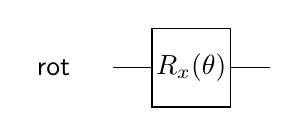
\begin{tikzpicture}[scale=.5] \node[draw=none] at (-3.5, 0) {rot}; \draw (-2,0) -- (-1, 0); \draw (1, 0) -- (2, 0); \draw (-1,-1)--(-1,1)--(1,1)--(1,-1)--cycle; \node[draw=none] at (0, 0) {$R_x(\theta)$}; \end{tikzpicture} } \]


\begin{DoxyParams}[1]{Parameters}
\mbox{\tt in,out}  & {\em multi\+Qubit} & object representing the set of all qubits \\
\hline
\mbox{\tt in}  & {\em rot\+Qubit} & qubit to rotate \\
\hline
\mbox{\tt in}  & {\em angle} & angle by which to rotate in radians \\
\hline
\end{DoxyParams}

\begin{DoxyExceptions}{Exceptions}
{\em exit\+With\+Error} & if {\ttfamily rot\+Qubit} is outside \mbox{[}0, {\ttfamily multi\+Qubit.\+num\+Qubits}). \\
\hline
\end{DoxyExceptions}


Definition at line 441 of file Qu\+E\+S\+T.\+c.



References rotate\+Around\+Axis().


\begin{DoxyCode}
441                                                                    \{
442 
443     \mbox{\hyperlink{structVector}{Vector}} unitAxis = \{1, 0, 0\};
444     \mbox{\hyperlink{QuEST_8c_a8810423457803005fecd415f4299f40d}{rotateAroundAxis}}(multiQubit, rotQubit, angle, unitAxis);
445 \}
\end{DoxyCode}
\mbox{\Hypertarget{QuEST_8h_ace0d3592d38a990e81a434c4e9681500}\label{QuEST_8h_ace0d3592d38a990e81a434c4e9681500}} 
\index{Qu\+E\+S\+T.\+h@{Qu\+E\+S\+T.\+h}!rotateY@{rotateY}}
\index{rotateY@{rotateY}!Qu\+E\+S\+T.\+h@{Qu\+E\+S\+T.\+h}}
\paragraph{\texorpdfstring{rotate\+Y()}{rotateY()}}
{\footnotesize\ttfamily void rotateY (\begin{DoxyParamCaption}\item[{\mbox{\hyperlink{structMultiQubit}{Multi\+Qubit}}}]{multi\+Qubit,  }\item[{const int}]{rot\+Qubit,  }\item[{\mbox{\hyperlink{QuEST__precision_8h_a4b654506f18b8bfd61ad2a29a7e38c25}{R\+E\+AL}}}]{angle }\end{DoxyParamCaption})}



Rotate a single qubit by a given angle around the Y-\/axis of the Bloch-\/sphere. 

For angle $\theta$, applies \[ \begin{pmatrix} \cos\theta/2 & - \sin \theta/2\\ \sin \theta/2 & \cos \theta/2 \end{pmatrix} \] ~\newline
 \[ \setlength{\fboxrule}{0.01pt} \fbox{ 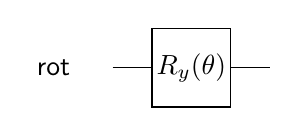
\begin{tikzpicture}[scale=.5] \node[draw=none] at (-3.5, 0) {rot}; \draw (-2,0) -- (-1, 0); \draw (1, 0) -- (2, 0); \draw (-1,-1)--(-1,1)--(1,1)--(1,-1)--cycle; \node[draw=none] at (0, 0) {$R_y(\theta)$}; \end{tikzpicture} } \]


\begin{DoxyParams}[1]{Parameters}
\mbox{\tt in,out}  & {\em multi\+Qubit} & object representing the set of all qubits \\
\hline
\mbox{\tt in}  & {\em rot\+Qubit} & qubit to rotate \\
\hline
\mbox{\tt in}  & {\em angle} & angle by which to rotate in radians \\
\hline
\end{DoxyParams}

\begin{DoxyExceptions}{Exceptions}
{\em exit\+With\+Error} & if {\ttfamily rot\+Qubit} is outside \mbox{[}0, {\ttfamily multi\+Qubit.\+num\+Qubits}). \\
\hline
\end{DoxyExceptions}


Definition at line 447 of file Qu\+E\+S\+T.\+c.



References rotate\+Around\+Axis().



Referenced by main().


\begin{DoxyCode}
447                                                                    \{
448 
449     \mbox{\hyperlink{structVector}{Vector}} unitAxis = \{0, 1, 0\};
450     \mbox{\hyperlink{QuEST_8c_a8810423457803005fecd415f4299f40d}{rotateAroundAxis}}(multiQubit, rotQubit, angle, unitAxis);
451 \}
\end{DoxyCode}
\mbox{\Hypertarget{QuEST_8h_abd621412ad30c1b034f4ce153c4afe10}\label{QuEST_8h_abd621412ad30c1b034f4ce153c4afe10}} 
\index{Qu\+E\+S\+T.\+h@{Qu\+E\+S\+T.\+h}!rotateZ@{rotateZ}}
\index{rotateZ@{rotateZ}!Qu\+E\+S\+T.\+h@{Qu\+E\+S\+T.\+h}}
\paragraph{\texorpdfstring{rotate\+Z()}{rotateZ()}}
{\footnotesize\ttfamily void rotateZ (\begin{DoxyParamCaption}\item[{\mbox{\hyperlink{structMultiQubit}{Multi\+Qubit}}}]{multi\+Qubit,  }\item[{const int}]{rot\+Qubit,  }\item[{\mbox{\hyperlink{QuEST__precision_8h_a4b654506f18b8bfd61ad2a29a7e38c25}{R\+E\+AL}}}]{angle }\end{DoxyParamCaption})}



Rotate a single qubit by a given angle around the Z-\/axis of the Bloch-\/sphere (also known as a phase shift gate). 

For angle $\theta$, applies \[ \begin{pmatrix} \exp(-i \theta/2) & 0 \\ 0 & \exp(i \theta/2) \end{pmatrix} \]

\[ \setlength{\fboxrule}{0.01pt} \fbox{ 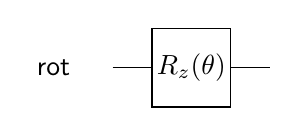
\begin{tikzpicture}[scale=.5] \node[draw=none] at (-3.5, 0) {rot}; \draw (-2,0) -- (-1, 0); \draw (1, 0) -- (2, 0); \draw (-1,-1)--(-1,1)--(1,1)--(1,-1)--cycle; \node[draw=none] at (0, 0) {$R_z(\theta)$}; \end{tikzpicture} } \]


\begin{DoxyParams}[1]{Parameters}
\mbox{\tt in,out}  & {\em multi\+Qubit} & object representing the set of all qubits \\
\hline
\mbox{\tt in}  & {\em rot\+Qubit} & qubit to rotate \\
\hline
\mbox{\tt in}  & {\em angle} & angle by which to rotate in radians \\
\hline
\end{DoxyParams}

\begin{DoxyExceptions}{Exceptions}
{\em exit\+With\+Error} & if {\ttfamily rot\+Qubit} is outside \mbox{[}0, {\ttfamily multi\+Qubit.\+num\+Qubits}). \\
\hline
\end{DoxyExceptions}


Definition at line 453 of file Qu\+E\+S\+T.\+c.



References rotate\+Around\+Axis().


\begin{DoxyCode}
453                                                                    \{
454 
455     \mbox{\hyperlink{structVector}{Vector}} unitAxis = \{0, 0, 1\};
456     \mbox{\hyperlink{QuEST_8c_a8810423457803005fecd415f4299f40d}{rotateAroundAxis}}(multiQubit, rotQubit, angle, unitAxis);
457 \}
\end{DoxyCode}
\mbox{\Hypertarget{QuEST_8h_a95012dad46509b4b461974c34cfd7b3d}\label{QuEST_8h_a95012dad46509b4b461974c34cfd7b3d}} 
\index{Qu\+E\+S\+T.\+h@{Qu\+E\+S\+T.\+h}!seed\+Qu\+E\+ST@{seed\+Qu\+E\+ST}}
\index{seed\+Qu\+E\+ST@{seed\+Qu\+E\+ST}!Qu\+E\+S\+T.\+h@{Qu\+E\+S\+T.\+h}}
\paragraph{\texorpdfstring{seed\+Qu\+E\+S\+T()}{seedQuEST()}}
{\footnotesize\ttfamily void seed\+Qu\+E\+ST (\begin{DoxyParamCaption}\item[{unsigned long int $\ast$}]{seed\+Array,  }\item[{int}]{num\+Seeds }\end{DoxyParamCaption})}



Seed the Mersenne Twister used for random number generation in the Qu\+E\+ST environment with a user defined seed. 

This function uses the mt19937 init\+\_\+by\+\_\+array function with num\+Seeds keys supplied by the user. Subsequent calls to mt19937 genrand functions will use this seeding. For a multi process code, the same seed is given to all process, therefore this seeding is only appropriate to use for functions such as measure where all processes require the same random value.


\begin{DoxyParams}[1]{Parameters}
\mbox{\tt in}  & {\em seed\+Array} & Array of integers to use as seed. This allows the MT to be initialised with more than a 32-\/bit integer if required \\
\hline
\mbox{\tt in}  & {\em num\+Seeds} & Length of seed\+Array\\
\hline
\end{DoxyParams}
For more information about the MT, see \href{http://www.math.sci.hiroshima-u.ac.jp/~m-mat/MT/MT2002/emt19937ar.html}{\tt http\+://www.\+math.\+sci.\+hiroshima-\/u.\+ac.\+jp/$\sim$m-\/mat/\+M\+T/\+M\+T2002/emt19937ar.\+html}

Seed the Mersenne Twister used for random number generation in the Qu\+E\+ST environment with a user defined seed. 

Definition at line 2019 of file Qu\+E\+S\+T.\+c.



References init\+\_\+by\+\_\+array().



Referenced by test\+\_\+measure().


\begin{DoxyCode}
2019                                                           \{
2020     \textcolor{comment}{// init MT random number generator with user defined list of seeds}
2021     \textcolor{comment}{// for the MPI version, it is ok that all procs will get the same seed as random numbers will only be }
2022     \textcolor{comment}{// used by the master process}
2023     \mbox{\hyperlink{mt19937ar_8c_ac1283f9b1ed571332f5ffe53545ffc16}{init\_by\_array}}(seedArray, numSeeds); 
2024 \}
\end{DoxyCode}
\mbox{\Hypertarget{QuEST_8h_aa8437ef3bf135231e2916e64dde1c94e}\label{QuEST_8h_aa8437ef3bf135231e2916e64dde1c94e}} 
\index{Qu\+E\+S\+T.\+h@{Qu\+E\+S\+T.\+h}!seed\+Qu\+E\+S\+T\+Default@{seed\+Qu\+E\+S\+T\+Default}}
\index{seed\+Qu\+E\+S\+T\+Default@{seed\+Qu\+E\+S\+T\+Default}!Qu\+E\+S\+T.\+h@{Qu\+E\+S\+T.\+h}}
\paragraph{\texorpdfstring{seed\+Qu\+E\+S\+T\+Default()}{seedQuESTDefault()}}
{\footnotesize\ttfamily void seed\+Qu\+E\+S\+T\+Default (\begin{DoxyParamCaption}\item[{void}]{ }\end{DoxyParamCaption})}



Seed the Mersenne Twister used for random number generation in the Qu\+E\+ST environment with an example defualt seed. 

This default seeding function uses the mt19937 init\+\_\+by\+\_\+array function with three keys -- time, pid and hostname. Subsequent calls to mt19937 genrand functions will use this seeding. For a multi process code, the same seed is given to all process, therefore this seeding is only appropriate to use for functions such as measure where all processes require the same random value.

For more information about the MT, see \href{http://www.math.sci.hiroshima-u.ac.jp/~m-mat/MT/MT2002/emt19937ar.html}{\tt http\+://www.\+math.\+sci.\+hiroshima-\/u.\+ac.\+jp/$\sim$m-\/mat/\+M\+T/\+M\+T2002/emt19937ar.\+html} 

Definition at line 1994 of file Qu\+E\+S\+T.\+c.



References hash\+String(), and init\+\_\+by\+\_\+array().



Referenced by init\+Qu\+E\+S\+T\+Env().


\begin{DoxyCode}
1994                        \{
1995     \textcolor{comment}{// init MT random number generator with three keys -- time, pid and a hash of hostname }
1996     \textcolor{comment}{// for the MPI version, it is ok that all procs will get the same seed as random numbers will only be }
1997     \textcolor{comment}{// used by the master process}
1998 
1999     \textcolor{keyword}{struct }timeval  tv;
2000     gettimeofday(&tv, NULL);
2001 
2002     \textcolor{keywordtype}{double} time\_in\_mill = 
2003         (tv.tv\_sec) * 1000 + (tv.tv\_usec) / 1000 ; \textcolor{comment}{// convert tv\_sec & tv\_usec to millisecond}
2004 
2005     \textcolor{keywordtype}{unsigned} \textcolor{keywordtype}{long} \textcolor{keywordtype}{int} pid = getpid();
2006     \textcolor{keywordtype}{unsigned} \textcolor{keywordtype}{long} \textcolor{keywordtype}{int} msecs = (\textcolor{keywordtype}{unsigned} \textcolor{keywordtype}{long} int) time\_in\_mill;
2007     \textcolor{keywordtype}{char} hostName[MAXHOSTNAMELEN+1];
2008     gethostname(hostName, \textcolor{keyword}{sizeof}(hostName));
2009     \textcolor{keywordtype}{unsigned} \textcolor{keywordtype}{long} \textcolor{keywordtype}{int} hostNameInt = \mbox{\hyperlink{QuEST_8c_ab76254cfde16f0808476649507a1a2fc}{hashString}}(hostName);
2010 
2011     \textcolor{keywordtype}{unsigned} \textcolor{keywordtype}{long} \textcolor{keywordtype}{int} key[3];
2012     key[0] = msecs; key[1] = pid; key[2] = hostNameInt;
2013     \mbox{\hyperlink{mt19937ar_8c_ac1283f9b1ed571332f5ffe53545ffc16}{init\_by\_array}}(key, 3); 
2014 \}
\end{DoxyCode}
\mbox{\Hypertarget{QuEST_8h_adda6c47876a7676488ed0565a19eaa65}\label{QuEST_8h_adda6c47876a7676488ed0565a19eaa65}} 
\index{Qu\+E\+S\+T.\+h@{Qu\+E\+S\+T.\+h}!s\+Gate@{s\+Gate}}
\index{s\+Gate@{s\+Gate}!Qu\+E\+S\+T.\+h@{Qu\+E\+S\+T.\+h}}
\paragraph{\texorpdfstring{s\+Gate()}{sGate()}}
{\footnotesize\ttfamily void s\+Gate (\begin{DoxyParamCaption}\item[{\mbox{\hyperlink{structMultiQubit}{Multi\+Qubit}}}]{multi\+Qubit,  }\item[{const int}]{target\+Qubit }\end{DoxyParamCaption})}



Apply the single-\/qubit S gate. 

This is a rotation of $\pi/2$ around the Z-\/axis on the Bloch sphere, or the unitary\+: \[ \begin{pmatrix} 1 & 0 \\ 0 & i \end{pmatrix} \]

\[ \setlength{\fboxrule}{0.01pt} \fbox{ 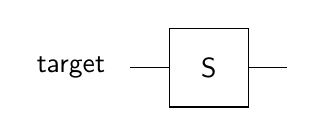
\begin{tikzpicture}[scale=.5] \node[draw=none] at (-3.5, 0) {target}; \draw (-2,0) -- (-1, 0); \draw (1, 0) -- (2, 0); \draw (-1,-1)--(-1,1)--(1,1)--(1,-1)--cycle; \node[draw=none] at (0, 0) {S}; \end{tikzpicture} } \]


\begin{DoxyParams}[1]{Parameters}
\mbox{\tt in,out}  & {\em multi\+Qubit} & object representing the set of all qubits \\
\hline
\mbox{\tt in}  & {\em target\+Qubit} & qubit to operate upon \\
\hline
\end{DoxyParams}

\begin{DoxyExceptions}{Exceptions}
{\em exit\+With\+Error} & if {\ttfamily target\+Qubit} is outside \mbox{[}0, {\ttfamily multi\+Qubit.\+num\+Qubits}) \\
\hline
\end{DoxyExceptions}


Definition at line 1626 of file Qu\+E\+S\+T.\+c.



References phase\+Gate(), and S\+\_\+\+G\+A\+TE.



Referenced by test\+\_\+s\+Gate().


\begin{DoxyCode}
1627 \{
1628     \mbox{\hyperlink{QuEST__env__local_8c_aae7a8a7f1ccbddb7f76b6c52b746bb43}{phaseGate}}(multiQubit, targetQubit, \mbox{\hyperlink{QuEST_8h_a5739021c733cecc49647956b2f7338eaa06e60f80fa80cce271793d6d31bcc21f}{S\_GATE}});
1629 \} 
\end{DoxyCode}
\mbox{\Hypertarget{QuEST_8h_a86e396e06b7d527cac20ba0108872423}\label{QuEST_8h_a86e396e06b7d527cac20ba0108872423}} 
\index{Qu\+E\+S\+T.\+h@{Qu\+E\+S\+T.\+h}!sigmaX@{sigmaX}}
\index{sigmaX@{sigmaX}!Qu\+E\+S\+T.\+h@{Qu\+E\+S\+T.\+h}}
\paragraph{\texorpdfstring{sigma\+X()}{sigmaX()}}
{\footnotesize\ttfamily void sigmaX (\begin{DoxyParamCaption}\item[{\mbox{\hyperlink{structMultiQubit}{Multi\+Qubit}}}]{multi\+Qubit,  }\item[{const int}]{target\+Qubit }\end{DoxyParamCaption})}



Apply the single-\/qubit sigma-\/X (also known as the X, Pauli-\/X, N\+OT or bit-\/flip) gate. 

This is a rotation of $\pi$ around the x-\/axis on the Bloch sphere. I.\+e. \[ \begin{pmatrix} 0 & 1 \\ 1 & 0 \end{pmatrix} \] ~\newline
 \[ \setlength{\fboxrule}{0.01pt} \fbox{ 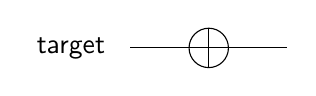
\begin{tikzpicture}[scale=.5] \node[draw=none] at (-3.5, 0) {target}; \draw (-2,0) -- (2, 0); \draw (0, 0) circle (.5); \draw (0, .5) -- (0, -.5); \end{tikzpicture} } \] ~\newline
 
\begin{DoxyParams}[1]{Parameters}
\mbox{\tt in,out}  & {\em multi\+Qubit} & object representing the set of all qubits \\
\hline
\mbox{\tt in}  & {\em target\+Qubit} & qubit to operate on \\
\hline
\end{DoxyParams}

\begin{DoxyExceptions}{Exceptions}
{\em exit\+With\+Error} & if {\ttfamily target\+Qubit} is outside \mbox{[}0, {\ttfamily multi\+Qubit.\+num\+Qubits}). \\
\hline
\end{DoxyExceptions}


Definition at line 151 of file Qu\+E\+S\+T\+\_\+env\+\_\+local.\+c.



References Multi\+Qubit\+::chunk\+Id, chunk\+Is\+Upper(), exchange\+State\+Vectors(), get\+Chunk\+Pair\+Id(), half\+Matrix\+Block\+Fits\+In\+Chunk(), Multi\+Qubit\+::num\+Amps\+Per\+Chunk, Multi\+Qubit\+::num\+Qubits, Multi\+Qubit\+::pair\+State\+Vec, Qu\+E\+S\+T\+Assert(), R\+E\+AL, sigma\+X\+Distributed(), sigma\+X\+Local(), and Multi\+Qubit\+::state\+Vec.



Referenced by main(), and test\+\_\+sigma\+X().


\begin{DoxyCode}
152 \{
153     \mbox{\hyperlink{QuEST__env__local_8c_a3587b9d533e633ccf1abf9ad2ce45d8d}{QuESTAssert}}(targetQubit >= 0 && targetQubit < multiQubit.
      \mbox{\hyperlink{structMultiQubit_ab5b9795bdc6fb5855e1974dcbbaeb36f}{numQubits}}, 1, \_\_func\_\_);
154     \mbox{\hyperlink{QuEST_8c_a74822fd86bb5d81766e6e8dbdcd62df1}{sigmaXLocal}}(multiQubit, targetQubit);
155 \}
\end{DoxyCode}
\mbox{\Hypertarget{QuEST_8h_a1f54d70a42403f7e1c2e2c2007332f61}\label{QuEST_8h_a1f54d70a42403f7e1c2e2c2007332f61}} 
\index{Qu\+E\+S\+T.\+h@{Qu\+E\+S\+T.\+h}!sigmaY@{sigmaY}}
\index{sigmaY@{sigmaY}!Qu\+E\+S\+T.\+h@{Qu\+E\+S\+T.\+h}}
\paragraph{\texorpdfstring{sigma\+Y()}{sigmaY()}}
{\footnotesize\ttfamily void sigmaY (\begin{DoxyParamCaption}\item[{\mbox{\hyperlink{structMultiQubit}{Multi\+Qubit}}}]{multi\+Qubit,  }\item[{const int}]{target\+Qubit }\end{DoxyParamCaption})}



Apply the single-\/qubit sigma-\/Y (also known as the Y or Pauli-\/Y) gate. 

This is a rotation of $\pi$ around the Y-\/axis on the Bloch sphere. I.\+e. \[ \begin{pmatrix} 0 & -i \\ i & 0 \end{pmatrix} \] ~\newline
 \[ \setlength{\fboxrule}{0.01pt} \fbox{ 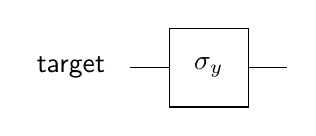
\begin{tikzpicture}[scale=.5] \node[draw=none] at (-3.5, 0) {target}; \draw (-2,0) -- (-1, 0); \draw (1, 0) -- (2, 0); \draw (-1,-1)--(-1,1)--(1,1)--(1,-1)--cycle; \node[draw=none] at (0, 0) {$\sigma_y$}; \end{tikzpicture} } \] ~\newline
 
\begin{DoxyParams}[1]{Parameters}
\mbox{\tt in,out}  & {\em multi\+Qubit} & object representing the set of all qubits \\
\hline
\mbox{\tt in}  & {\em target\+Qubit} & qubit to operate on \\
\hline
\end{DoxyParams}

\begin{DoxyExceptions}{Exceptions}
{\em exit\+With\+Error} & if {\ttfamily target\+Qubit} is outside \mbox{[}0, {\ttfamily multi\+Qubit.\+num\+Qubits}). \\
\hline
\end{DoxyExceptions}
fix -- put duplicate code (sigmaX, sigmaY) in seperate function 

Definition at line 157 of file Qu\+E\+S\+T\+\_\+env\+\_\+local.\+c.



References Multi\+Qubit\+::chunk\+Id, chunk\+Is\+Upper(), exchange\+State\+Vectors(), get\+Chunk\+Pair\+Id(), half\+Matrix\+Block\+Fits\+In\+Chunk(), Multi\+Qubit\+::num\+Amps\+Per\+Chunk, Multi\+Qubit\+::num\+Qubits, Multi\+Qubit\+::pair\+State\+Vec, Qu\+E\+S\+T\+Assert(), R\+E\+AL, sigma\+Y\+Distributed(), sigma\+Y\+Local(), and Multi\+Qubit\+::state\+Vec.



Referenced by test\+\_\+sigma\+Y().


\begin{DoxyCode}
158 \{
159     \mbox{\hyperlink{QuEST__env__local_8c_a3587b9d533e633ccf1abf9ad2ce45d8d}{QuESTAssert}}(targetQubit >= 0 && targetQubit < multiQubit.
      \mbox{\hyperlink{structMultiQubit_ab5b9795bdc6fb5855e1974dcbbaeb36f}{numQubits}}, 1, \_\_func\_\_);
160     \mbox{\hyperlink{QuEST_8c_a81fbfaed65a742a7dfd622e17652245e}{sigmaYLocal}}(multiQubit, targetQubit);
161 \}
\end{DoxyCode}
\mbox{\Hypertarget{QuEST_8h_aebaab86326779de55d335cfea3efde8f}\label{QuEST_8h_aebaab86326779de55d335cfea3efde8f}} 
\index{Qu\+E\+S\+T.\+h@{Qu\+E\+S\+T.\+h}!sigmaZ@{sigmaZ}}
\index{sigmaZ@{sigmaZ}!Qu\+E\+S\+T.\+h@{Qu\+E\+S\+T.\+h}}
\paragraph{\texorpdfstring{sigma\+Z()}{sigmaZ()}}
{\footnotesize\ttfamily void sigmaZ (\begin{DoxyParamCaption}\item[{\mbox{\hyperlink{structMultiQubit}{Multi\+Qubit}}}]{multi\+Qubit,  }\item[{const int}]{target\+Qubit }\end{DoxyParamCaption})}



Apply the single-\/qubit sigma-\/Z (also known as the Z, Pauli-\/Z or phase-\/flip) gate. 

This is a rotation of $\pi$ around the Z-\/axis (a phase shift) on the Bloch sphere. I.\+e. \[ \begin{pmatrix} 1 & 0 \\ 0 & -1 \end{pmatrix} \] ~\newline
 \[ \setlength{\fboxrule}{0.01pt} \fbox{ 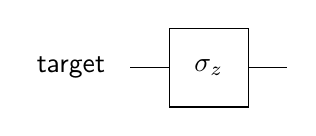
\begin{tikzpicture}[scale=.5] \node[draw=none] at (-3.5, 0) {target}; \draw (-2,0) -- (-1, 0); \draw (1, 0) -- (2, 0); \draw (-1,-1)--(-1,1)--(1,1)--(1,-1)--cycle; \node[draw=none] at (0, 0) {$\sigma_z$}; \end{tikzpicture} } \] ~\newline
 
\begin{DoxyParams}[1]{Parameters}
\mbox{\tt in,out}  & {\em multi\+Qubit} & object representing the set of all qubits \\
\hline
\mbox{\tt in}  & {\em target\+Qubit} & qubit to operate on \\
\hline
\end{DoxyParams}

\begin{DoxyExceptions}{Exceptions}
{\em exit\+With\+Error} & if {\ttfamily target\+Qubit} is outside \mbox{[}0, {\ttfamily multi\+Qubit.\+num\+Qubits}). \\
\hline
\end{DoxyExceptions}


Definition at line 1621 of file Qu\+E\+S\+T.\+c.



References phase\+Gate(), and S\+I\+G\+M\+A\+\_\+Z.



Referenced by test\+\_\+sigma\+Z().


\begin{DoxyCode}
1622 \{
1623     \mbox{\hyperlink{QuEST__env__local_8c_aae7a8a7f1ccbddb7f76b6c52b746bb43}{phaseGate}}(multiQubit, targetQubit, \mbox{\hyperlink{QuEST_8h_a5739021c733cecc49647956b2f7338eaa754922d1e1846a1961ff2bf163483dac}{SIGMA\_Z}});
1624 \}
\end{DoxyCode}
\mbox{\Hypertarget{QuEST_8h_a8d31fe2d1ad4d01e2a1f5f6b8bc15b77}\label{QuEST_8h_a8d31fe2d1ad4d01e2a1f5f6b8bc15b77}} 
\index{Qu\+E\+S\+T.\+h@{Qu\+E\+S\+T.\+h}!sync\+Qu\+E\+S\+T\+Env@{sync\+Qu\+E\+S\+T\+Env}}
\index{sync\+Qu\+E\+S\+T\+Env@{sync\+Qu\+E\+S\+T\+Env}!Qu\+E\+S\+T.\+h@{Qu\+E\+S\+T.\+h}}
\paragraph{\texorpdfstring{sync\+Qu\+E\+S\+T\+Env()}{syncQuESTEnv()}}
{\footnotesize\ttfamily void sync\+Qu\+E\+S\+T\+Env (\begin{DoxyParamCaption}\item[{\mbox{\hyperlink{structQuESTEnv}{Qu\+E\+S\+T\+Env}}}]{env }\end{DoxyParamCaption})}



Guarantees that all code up to the given point has been executed on all nodes (if running in distributed mode) 


\begin{DoxyParams}[1]{Parameters}
\mbox{\tt in}  & {\em env} & object representing the execution environment. A single instance is used for each program \\
\hline
\end{DoxyParams}


Definition at line 31 of file Qu\+E\+S\+T\+\_\+env\+\_\+local.\+c.



Referenced by initialize\+State\+From\+Single\+File(), report\+State\+To\+Screen(), and test\+\_\+controlled\+Not().


\begin{DoxyCode}
31                                \{
32     \textcolor{comment}{// MPI Barrier goes here in MPI version. }
33 \} 
\end{DoxyCode}
\mbox{\Hypertarget{QuEST_8h_ac7e38d768a1bd79019f88cc1e6295092}\label{QuEST_8h_ac7e38d768a1bd79019f88cc1e6295092}} 
\index{Qu\+E\+S\+T.\+h@{Qu\+E\+S\+T.\+h}!sync\+Qu\+E\+S\+T\+Success@{sync\+Qu\+E\+S\+T\+Success}}
\index{sync\+Qu\+E\+S\+T\+Success@{sync\+Qu\+E\+S\+T\+Success}!Qu\+E\+S\+T.\+h@{Qu\+E\+S\+T.\+h}}
\paragraph{\texorpdfstring{sync\+Qu\+E\+S\+T\+Success()}{syncQuESTSuccess()}}
{\footnotesize\ttfamily int sync\+Qu\+E\+S\+T\+Success (\begin{DoxyParamCaption}\item[{int}]{success\+Code }\end{DoxyParamCaption})}



Performs a logical A\+ND on all success\+Codes held by all processes. 

If any one process has a zero success\+Code all processes will return a zero success code.


\begin{DoxyParams}[1]{Parameters}
\mbox{\tt in}  & {\em env} & object representing the execution environment. A single instance is used for each program \\
\hline
\mbox{\tt in}  & {\em success\+Code} & 1 if process task succeeded, 0 if process task failed \\
\hline
\end{DoxyParams}
\begin{DoxyReturn}{Returns}
1 if all processes succeeded, 0 if any one process failed 
\end{DoxyReturn}


Definition at line 35 of file Qu\+E\+S\+T\+\_\+env\+\_\+local.\+c.



Referenced by main().


\begin{DoxyCode}
35                                      \{
36     \textcolor{keywordflow}{return} successCode;
37 \}
\end{DoxyCode}
\mbox{\Hypertarget{QuEST_8h_af764ea63a2e870098f4e1ce08562942e}\label{QuEST_8h_af764ea63a2e870098f4e1ce08562942e}} 
\index{Qu\+E\+S\+T.\+h@{Qu\+E\+S\+T.\+h}!t\+Gate@{t\+Gate}}
\index{t\+Gate@{t\+Gate}!Qu\+E\+S\+T.\+h@{Qu\+E\+S\+T.\+h}}
\paragraph{\texorpdfstring{t\+Gate()}{tGate()}}
{\footnotesize\ttfamily void t\+Gate (\begin{DoxyParamCaption}\item[{\mbox{\hyperlink{structMultiQubit}{Multi\+Qubit}}}]{multi\+Qubit,  }\item[{const int}]{target\+Qubit }\end{DoxyParamCaption})}



Apply the single-\/qubit T gate. 

This is a rotation of $\pi/4$ around the Z-\/axis on the Bloch sphere, or the unitary\+: \[ \begin{pmatrix} 1 & 0 \\ 0 & \exp\left(i \frac{\pi}{4}\right) \end{pmatrix} \]

\[ \setlength{\fboxrule}{0.01pt} \fbox{ 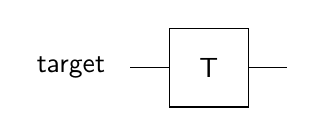
\begin{tikzpicture}[scale=.5] \node[draw=none] at (-3.5, 0) {target}; \draw (-2,0) -- (-1, 0); \draw (1, 0) -- (2, 0); \draw (-1,-1)--(-1,1)--(1,1)--(1,-1)--cycle; \node[draw=none] at (0, 0) {T}; \end{tikzpicture} } \]


\begin{DoxyParams}[1]{Parameters}
\mbox{\tt in,out}  & {\em multi\+Qubit} & object representing the set of all qubits \\
\hline
\mbox{\tt in}  & {\em target\+Qubit} & qubit to operate upon \\
\hline
\end{DoxyParams}

\begin{DoxyExceptions}{Exceptions}
{\em exit\+With\+Error} & if {\ttfamily target\+Qubit} is outside \mbox{[}0, {\ttfamily multi\+Qubit.\+num\+Qubits}) \\
\hline
\end{DoxyExceptions}


Definition at line 1631 of file Qu\+E\+S\+T.\+c.



References phase\+Gate(), and T\+\_\+\+G\+A\+TE.



Referenced by test\+\_\+t\+Gate().


\begin{DoxyCode}
1632 \{
1633     \mbox{\hyperlink{QuEST__env__local_8c_aae7a8a7f1ccbddb7f76b6c52b746bb43}{phaseGate}}(multiQubit, targetQubit, \mbox{\hyperlink{QuEST_8h_a5739021c733cecc49647956b2f7338eaa614d07d597a8e320cc556bc0e652e4ab}{T\_GATE}});
1634 \}
\end{DoxyCode}
\mbox{\Hypertarget{QuEST_8h_a7a0877e33700f6bad48adb51b7b3fb67}\label{QuEST_8h_a7a0877e33700f6bad48adb51b7b3fb67}} 
\index{Qu\+E\+S\+T.\+h@{Qu\+E\+S\+T.\+h}!unitary@{unitary}}
\index{unitary@{unitary}!Qu\+E\+S\+T.\+h@{Qu\+E\+S\+T.\+h}}
\paragraph{\texorpdfstring{unitary()}{unitary()}}
{\footnotesize\ttfamily void unitary (\begin{DoxyParamCaption}\item[{\mbox{\hyperlink{structMultiQubit}{Multi\+Qubit}}}]{multi\+Qubit,  }\item[{const int}]{target\+Qubit,  }\item[{\mbox{\hyperlink{structComplexMatrix2}{Complex\+Matrix2}}}]{u }\end{DoxyParamCaption})}



Apply a general single-\/qubit unitary (including a global phase factor). 

The passed 2x2 Complex\+Matrix must be unitary, otherwise an error is thrown.

\[ \setlength{\fboxrule}{0.01pt} \fbox{ 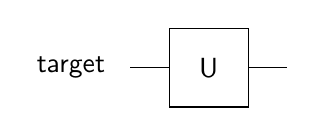
\begin{tikzpicture}[scale=.5] \node[draw=none] at (-3.5, 0) {target}; \draw (-2,0) -- (-1, 0); \draw (1, 0) -- (2, 0); \draw (-1,-1)--(-1,1)--(1,1)--(1,-1)--cycle; \node[draw=none] at (0, 0) {U}; \end{tikzpicture} } \]


\begin{DoxyParams}[1]{Parameters}
\mbox{\tt in,out}  & {\em multi\+Qubit} & object representing the set of all qubits \\
\hline
\mbox{\tt in}  & {\em target\+Qubit} & qubit to operate on \\
\hline
\mbox{\tt in}  & {\em u} & unitary matrix to apply \\
\hline
\end{DoxyParams}

\begin{DoxyExceptions}{Exceptions}
{\em exit\+With\+Error} & if {\ttfamily target\+Qubit} is outside \mbox{[}0, {\ttfamily multi\+Qubit.\+num\+Qubits}), or matrix {\ttfamily u} is not unitary. \\
\hline
\end{DoxyExceptions}


Definition at line 107 of file Qu\+E\+S\+T\+\_\+env\+\_\+local.\+c.



References Multi\+Qubit\+::chunk\+Id, chunk\+Is\+Upper(), exchange\+State\+Vectors(), get\+Chunk\+Pair\+Id(), get\+Rot\+Angle\+From\+Unitary\+Matrix(), half\+Matrix\+Block\+Fits\+In\+Chunk(), Multi\+Qubit\+::num\+Amps\+Per\+Chunk, Multi\+Qubit\+::num\+Qubits, Multi\+Qubit\+::pair\+State\+Vec, Qu\+E\+S\+T\+Assert(), R\+E\+AL, Multi\+Qubit\+::state\+Vec, unitary\+Distributed(), unitary\+Local(), and validate\+Matrix\+Is\+Unitary().



Referenced by main(), and test\+\_\+unitary().


\begin{DoxyCode}
108 \{
109     \mbox{\hyperlink{QuEST__env__local_8c_a3587b9d533e633ccf1abf9ad2ce45d8d}{QuESTAssert}}(targetQubit >= 0 && targetQubit < multiQubit.
      \mbox{\hyperlink{structMultiQubit_ab5b9795bdc6fb5855e1974dcbbaeb36f}{numQubits}}, 1, \_\_func\_\_);
110     \mbox{\hyperlink{QuEST__env__local_8c_a3587b9d533e633ccf1abf9ad2ce45d8d}{QuESTAssert}}(\mbox{\hyperlink{QuEST_8c_ae4fea133d1a8f09ff8da03038100adb2}{validateMatrixIsUnitary}}(u), 5, \_\_func\_\_);
111 
112     \textcolor{comment}{// all values required to update state vector lie in this rank}
113     \mbox{\hyperlink{QuEST_8c_ac134fb45b0a7248c5d15e16eb7139a35}{unitaryLocal}}(multiQubit, targetQubit, u);
114 \}
\end{DoxyCode}

\hypertarget{QuEST__debug_8h}{}\subsection{Qu\+E\+S\+T\+\_\+debug.\+h File Reference}
\label{QuEST__debug_8h}\index{Qu\+E\+S\+T\+\_\+debug.\+h@{Qu\+E\+S\+T\+\_\+debug.\+h}}


Developer functions used for unit testing and debugging.  


{\ttfamily \#include \char`\"{}Qu\+E\+S\+T\+\_\+precision.\+h\char`\"{}}\newline
\subsubsection*{Functions}
\begin{DoxyCompactItemize}
\item 
void \mbox{\hyperlink{QuEST__debug_8h_a7169fd0442cbc3418f3fac4d13363ca2}{init\+State\+Of\+Single\+Qubit}} (\mbox{\hyperlink{structMultiQubit}{Multi\+Qubit}} $\ast$multi\+Qubit, int qubit\+Id, int outcome)
\begin{DoxyCompactList}\small\item\em Initialise the state vector of probability amplitudes such that one qubit is set to \textquotesingle{}outcome\textquotesingle{} and all other qubits are in an equal superposition of zero and one. \end{DoxyCompactList}\item 
void \mbox{\hyperlink{QuEST__debug_8h_a03b3577a891731d505bc4b879fcca9d3}{init\+State\+Debug}} (\mbox{\hyperlink{structMultiQubit}{Multi\+Qubit}} $\ast$multi\+Qubit)
\begin{DoxyCompactList}\small\item\em Initialise the state vector of probability amplitudes to an (unphysical) state with each component of each probability amplitude a unique floating point value. \end{DoxyCompactList}\item 
void \mbox{\hyperlink{QuEST__debug_8h_a433876ee9f3bcc54af346300f571fc3c}{initialize\+State\+From\+Single\+File}} (\mbox{\hyperlink{structMultiQubit}{Multi\+Qubit}} $\ast$multi\+Qubit, char filename\mbox{[}200\mbox{]}, \mbox{\hyperlink{structQuESTEnv}{Qu\+E\+S\+T\+Env}} env)
\item 
int \mbox{\hyperlink{QuEST__debug_8h_a793584932ae384c82e7e42db7d35d18d}{compare\+States}} (\mbox{\hyperlink{structMultiQubit}{Multi\+Qubit}} mq1, \mbox{\hyperlink{structMultiQubit}{Multi\+Qubit}} mq2, \mbox{\hyperlink{QuEST__precision_8h_a4b654506f18b8bfd61ad2a29a7e38c25}{R\+E\+AL}} precision)
\item 
void \mbox{\hyperlink{QuEST__debug_8h_a62da5b58d8ce84e6f4d24be1b872294e}{report\+Node\+List}} (\mbox{\hyperlink{structQuESTEnv}{Qu\+E\+S\+T\+Env}} env)
\begin{DoxyCompactList}\small\item\em Report a list of C\+PU hostnames and the rank that is running on each if running with M\+PI enabled and an error message otherwise. \end{DoxyCompactList}\end{DoxyCompactItemize}


\subsubsection{Detailed Description}
Developer functions used for unit testing and debugging. 

Not part of the public A\+PI. May contain functions that are incomplete or untested. 

\subsubsection{Function Documentation}
\mbox{\Hypertarget{QuEST__debug_8h_a793584932ae384c82e7e42db7d35d18d}\label{QuEST__debug_8h_a793584932ae384c82e7e42db7d35d18d}} 
\index{Qu\+E\+S\+T\+\_\+debug.\+h@{Qu\+E\+S\+T\+\_\+debug.\+h}!compare\+States@{compare\+States}}
\index{compare\+States@{compare\+States}!Qu\+E\+S\+T\+\_\+debug.\+h@{Qu\+E\+S\+T\+\_\+debug.\+h}}
\paragraph{\texorpdfstring{compare\+States()}{compareStates()}}
{\footnotesize\ttfamily int compare\+States (\begin{DoxyParamCaption}\item[{\mbox{\hyperlink{structMultiQubit}{Multi\+Qubit}}}]{mq1,  }\item[{\mbox{\hyperlink{structMultiQubit}{Multi\+Qubit}}}]{mq2,  }\item[{\mbox{\hyperlink{QuEST__precision_8h_a4b654506f18b8bfd61ad2a29a7e38c25}{R\+E\+AL}}}]{precision }\end{DoxyParamCaption})}



Definition at line 372 of file Qu\+E\+S\+T.\+c.



References Complex\+Array\+::imag, Multi\+Qubit\+::num\+Amps, Complex\+Array\+::real, R\+E\+AL, and Multi\+Qubit\+::state\+Vec.


\begin{DoxyCode}
372                                                                  \{
373     \mbox{\hyperlink{QuEST__precision_8h_a4b654506f18b8bfd61ad2a29a7e38c25}{REAL}} diff;
374     \textcolor{keywordtype}{int} chunkSize = mq1.\mbox{\hyperlink{structMultiQubit_ae16f47d8b725c914fb7f66b6498d79db}{numAmps}};
375     \textcolor{keywordflow}{for} (\textcolor{keywordtype}{int} i=0; i<chunkSize; i++)\{
376         diff = fabs(mq1.\mbox{\hyperlink{structMultiQubit_a45483190d6b01ef6b2f98f2bec9ab94f}{stateVec}}.\mbox{\hyperlink{structComplexArray_a4195cac6c784ea1b6271f1c7dba1548a}{real}}[i] - mq2.\mbox{\hyperlink{structMultiQubit_a45483190d6b01ef6b2f98f2bec9ab94f}{stateVec}}.\mbox{\hyperlink{structComplexArray_a4195cac6c784ea1b6271f1c7dba1548a}{real}}[i]);
377         \textcolor{keywordflow}{if} (diff>precision) \textcolor{keywordflow}{return} 0;
378         diff = fabs(mq1.\mbox{\hyperlink{structMultiQubit_a45483190d6b01ef6b2f98f2bec9ab94f}{stateVec}}.\mbox{\hyperlink{structComplexArray_a79dde47c7ae530c79cebfdf57b225968}{imag}}[i] - mq2.\mbox{\hyperlink{structMultiQubit_a45483190d6b01ef6b2f98f2bec9ab94f}{stateVec}}.\mbox{\hyperlink{structComplexArray_a79dde47c7ae530c79cebfdf57b225968}{imag}}[i]);
379         \textcolor{keywordflow}{if} (diff>precision) \textcolor{keywordflow}{return} 0;
380     \}
381     \textcolor{keywordflow}{return} 1;
382 \}
\end{DoxyCode}
\mbox{\Hypertarget{QuEST__debug_8h_a433876ee9f3bcc54af346300f571fc3c}\label{QuEST__debug_8h_a433876ee9f3bcc54af346300f571fc3c}} 
\index{Qu\+E\+S\+T\+\_\+debug.\+h@{Qu\+E\+S\+T\+\_\+debug.\+h}!initialize\+State\+From\+Single\+File@{initialize\+State\+From\+Single\+File}}
\index{initialize\+State\+From\+Single\+File@{initialize\+State\+From\+Single\+File}!Qu\+E\+S\+T\+\_\+debug.\+h@{Qu\+E\+S\+T\+\_\+debug.\+h}}
\paragraph{\texorpdfstring{initialize\+State\+From\+Single\+File()}{initializeStateFromSingleFile()}}
{\footnotesize\ttfamily void initialize\+State\+From\+Single\+File (\begin{DoxyParamCaption}\item[{\mbox{\hyperlink{structMultiQubit}{Multi\+Qubit}} $\ast$}]{multi\+Qubit,  }\item[{char}]{filename\mbox{[}200\mbox{]},  }\item[{\mbox{\hyperlink{structQuESTEnv}{Qu\+E\+S\+T\+Env}}}]{env }\end{DoxyParamCaption})}

fix -- format needs to work for single precision values 

Definition at line 336 of file Qu\+E\+S\+T.\+c.



References Multi\+Qubit\+::chunk\+Id, Complex\+Array\+::imag, Multi\+Qubit\+::num\+Amps, Multi\+Qubit\+::num\+Chunks, Qu\+E\+S\+T\+Assert(), Complex\+Array\+::real, R\+E\+AL, Multi\+Qubit\+::state\+Vec, and sync\+Qu\+E\+S\+T\+Env().


\begin{DoxyCode}
336                                                                                             \{
337     \textcolor{keywordtype}{long} \textcolor{keywordtype}{long} \textcolor{keywordtype}{int} chunkSize, stateVecSize;
338     \textcolor{keywordtype}{long} \textcolor{keywordtype}{long} \textcolor{keywordtype}{int} indexInChunk, totalIndex;
339 
340     chunkSize = multiQubit->\mbox{\hyperlink{structMultiQubit_ae16f47d8b725c914fb7f66b6498d79db}{numAmps}};
341     stateVecSize = chunkSize*multiQubit->\mbox{\hyperlink{structMultiQubit_acd43f2f57991709c9e94f73662c972b2}{numChunks}};
342 
343     \mbox{\hyperlink{QuEST__precision_8h_a4b654506f18b8bfd61ad2a29a7e38c25}{REAL}} *stateVecReal = multiQubit->\mbox{\hyperlink{structMultiQubit_a45483190d6b01ef6b2f98f2bec9ab94f}{stateVec}}.\mbox{\hyperlink{structComplexArray_a4195cac6c784ea1b6271f1c7dba1548a}{real}};
344     \mbox{\hyperlink{QuEST__precision_8h_a4b654506f18b8bfd61ad2a29a7e38c25}{REAL}} *stateVecImag = multiQubit->\mbox{\hyperlink{structMultiQubit_a45483190d6b01ef6b2f98f2bec9ab94f}{stateVec}}.\mbox{\hyperlink{structComplexArray_a79dde47c7ae530c79cebfdf57b225968}{imag}};
345 
346     FILE *fp;
347     \textcolor{keywordtype}{char} line[200];
348 
349     \textcolor{keywordflow}{for} (\textcolor{keywordtype}{int} rank=0; rank<(multiQubit->\mbox{\hyperlink{structMultiQubit_acd43f2f57991709c9e94f73662c972b2}{numChunks}}); rank++)\{
350         \textcolor{keywordflow}{if} (rank==multiQubit->\mbox{\hyperlink{structMultiQubit_ab10c88249fa3825d6227ceec01d37e37}{chunkId}})\{
351             fp = fopen(filename, \textcolor{stringliteral}{"r"});
352             \mbox{\hyperlink{QuEST__env__local_8c_a3587b9d533e633ccf1abf9ad2ce45d8d}{QuESTAssert}}(fp!=NULL, 11, \_\_func\_\_);
353             indexInChunk = 0; totalIndex = 0;
354             \textcolor{keywordflow}{while} (fgets(line, \textcolor{keyword}{sizeof}(\textcolor{keywordtype}{char})*200, fp) != NULL && totalIndex<stateVecSize)\{
355                 \textcolor{keywordflow}{if} (line[0]!=\textcolor{charliteral}{'#'})\{
356                     \textcolor{keywordtype}{int} chunkId = totalIndex/chunkSize;
357                     \textcolor{keywordflow}{if} (chunkId==multiQubit->\mbox{\hyperlink{structMultiQubit_ab10c88249fa3825d6227ceec01d37e37}{chunkId}})\{
359                         sscanf(line, \textcolor{stringliteral}{"%lf, %lf"}, &(stateVecReal[indexInChunk]), 
360                                 &(stateVecImag[indexInChunk]));
361                         indexInChunk += 1;
362                     \}
363                     totalIndex += 1;
364                 \}
365             \}   
366             fclose(fp);
367         \}
368         \mbox{\hyperlink{QuEST_8h_a8d31fe2d1ad4d01e2a1f5f6b8bc15b77}{syncQuESTEnv}}(env);
369     \}
370 \}
\end{DoxyCode}
\mbox{\Hypertarget{QuEST__debug_8h_a03b3577a891731d505bc4b879fcca9d3}\label{QuEST__debug_8h_a03b3577a891731d505bc4b879fcca9d3}} 
\index{Qu\+E\+S\+T\+\_\+debug.\+h@{Qu\+E\+S\+T\+\_\+debug.\+h}!init\+State\+Debug@{init\+State\+Debug}}
\index{init\+State\+Debug@{init\+State\+Debug}!Qu\+E\+S\+T\+\_\+debug.\+h@{Qu\+E\+S\+T\+\_\+debug.\+h}}
\paragraph{\texorpdfstring{init\+State\+Debug()}{initStateDebug()}}
{\footnotesize\ttfamily void init\+State\+Debug (\begin{DoxyParamCaption}\item[{\mbox{\hyperlink{structMultiQubit}{Multi\+Qubit}} $\ast$}]{multi\+Qubit }\end{DoxyParamCaption})}



Initialise the state vector of probability amplitudes to an (unphysical) state with each component of each probability amplitude a unique floating point value. 

For debugging processes 
\begin{DoxyParams}[1]{Parameters}
\mbox{\tt in,out}  & {\em multi\+Qubit} & object representing the set of qubits to be initialised \\
\hline
\end{DoxyParams}


Definition at line 304 of file Qu\+E\+S\+T.\+c.



References Multi\+Qubit\+::chunk\+Id, Complex\+Array\+::imag, Multi\+Qubit\+::num\+Amps, Complex\+Array\+::real, R\+E\+AL, and Multi\+Qubit\+::state\+Vec.


\begin{DoxyCode}
305 \{
306     \textcolor{keywordtype}{long} \textcolor{keywordtype}{long} \textcolor{keywordtype}{int} chunkSize;
307     \textcolor{keywordtype}{long} \textcolor{keywordtype}{long} \textcolor{keywordtype}{int} index;
308 
309     \textcolor{comment}{// dimension of the state vector}
310     chunkSize = multiQubit->\mbox{\hyperlink{structMultiQubit_ae16f47d8b725c914fb7f66b6498d79db}{numAmps}};
311 
312     \textcolor{comment}{// Can't use multiQubit->stateVec as a private OMP var}
313     \mbox{\hyperlink{QuEST__precision_8h_a4b654506f18b8bfd61ad2a29a7e38c25}{REAL}} *stateVecReal = multiQubit->\mbox{\hyperlink{structMultiQubit_a45483190d6b01ef6b2f98f2bec9ab94f}{stateVec}}.\mbox{\hyperlink{structComplexArray_a4195cac6c784ea1b6271f1c7dba1548a}{real}};
314     \mbox{\hyperlink{QuEST__precision_8h_a4b654506f18b8bfd61ad2a29a7e38c25}{REAL}} *stateVecImag = multiQubit->\mbox{\hyperlink{structMultiQubit_a45483190d6b01ef6b2f98f2bec9ab94f}{stateVec}}.\mbox{\hyperlink{structComplexArray_a79dde47c7ae530c79cebfdf57b225968}{imag}};
315 
316     \mbox{\hyperlink{QuEST__precision_8h_a4b654506f18b8bfd61ad2a29a7e38c25}{REAL}} chunkOffset = (2.0*chunkSize*multiQubit->\mbox{\hyperlink{structMultiQubit_ab10c88249fa3825d6227ceec01d37e37}{chunkId}})/10.0;
317 
318     \textcolor{comment}{// initialise the state to |0000..0000>}
319 \textcolor{preprocessor}{# ifdef \_OPENMP}
320 \textcolor{preprocessor}{# pragma omp parallel \(\backslash\)}
321 \textcolor{preprocessor}{    default  (none) \(\backslash\)}
322 \textcolor{preprocessor}{    shared   (chunkSize, stateVecReal, stateVecImag, chunkOffset) \(\backslash\)}
323 \textcolor{preprocessor}{    private  (index) }
324 \textcolor{preprocessor}{# endif}
325     \{
326 \textcolor{preprocessor}{# ifdef \_OPENMP}
327 \textcolor{preprocessor}{# pragma omp for schedule (static)}
328 \textcolor{preprocessor}{# endif}
329         \textcolor{keywordflow}{for} (index=0; index<chunkSize; index++) \{
330             stateVecReal[index] = chunkOffset + (index*2.0)/10.0;
331             stateVecImag[index] = chunkOffset + (index*2.0+1.0)/10.0;
332         \}
333     \}
334 \}
\end{DoxyCode}
\mbox{\Hypertarget{QuEST__debug_8h_a7169fd0442cbc3418f3fac4d13363ca2}\label{QuEST__debug_8h_a7169fd0442cbc3418f3fac4d13363ca2}} 
\index{Qu\+E\+S\+T\+\_\+debug.\+h@{Qu\+E\+S\+T\+\_\+debug.\+h}!init\+State\+Of\+Single\+Qubit@{init\+State\+Of\+Single\+Qubit}}
\index{init\+State\+Of\+Single\+Qubit@{init\+State\+Of\+Single\+Qubit}!Qu\+E\+S\+T\+\_\+debug.\+h@{Qu\+E\+S\+T\+\_\+debug.\+h}}
\paragraph{\texorpdfstring{init\+State\+Of\+Single\+Qubit()}{initStateOfSingleQubit()}}
{\footnotesize\ttfamily void init\+State\+Of\+Single\+Qubit (\begin{DoxyParamCaption}\item[{\mbox{\hyperlink{structMultiQubit}{Multi\+Qubit}} $\ast$}]{multi\+Qubit,  }\item[{int}]{qubit\+Id,  }\item[{int}]{outcome }\end{DoxyParamCaption})}



Initialise the state vector of probability amplitudes such that one qubit is set to \textquotesingle{}outcome\textquotesingle{} and all other qubits are in an equal superposition of zero and one. 


\begin{DoxyParams}[1]{Parameters}
\mbox{\tt in,out}  & {\em multi\+Qubit} & object representing the set of qubits to be initialised \\
\hline
\mbox{\tt in}  & {\em qubit\+Id} & id of qubit to set to state \textquotesingle{}outcome\textquotesingle{} \\
\hline
\mbox{\tt in}  & {\em value} & of qubit \textquotesingle{}qubit\+Id\textquotesingle{} \\
\hline
\end{DoxyParams}


Definition at line 258 of file Qu\+E\+S\+T.\+c.



References Multi\+Qubit\+::chunk\+Id, extract\+Bit(), Complex\+Array\+::imag, Multi\+Qubit\+::num\+Amps, Multi\+Qubit\+::num\+Chunks, Complex\+Array\+::real, R\+E\+AL, and Multi\+Qubit\+::state\+Vec.


\begin{DoxyCode}
259 \{
260     \textcolor{keywordtype}{long} \textcolor{keywordtype}{long} \textcolor{keywordtype}{int} chunkSize, stateVecSize;
261     \textcolor{keywordtype}{long} \textcolor{keywordtype}{long} \textcolor{keywordtype}{int} index;
262     \textcolor{keywordtype}{int} bit;
263     \textcolor{keyword}{const} \textcolor{keywordtype}{long} \textcolor{keywordtype}{long} \textcolor{keywordtype}{int} chunkId=multiQubit->\mbox{\hyperlink{structMultiQubit_ab10c88249fa3825d6227ceec01d37e37}{chunkId}};
264 
265     \textcolor{comment}{// dimension of the state vector}
266     chunkSize = multiQubit->\mbox{\hyperlink{structMultiQubit_ae16f47d8b725c914fb7f66b6498d79db}{numAmps}};
267     stateVecSize = chunkSize*multiQubit->\mbox{\hyperlink{structMultiQubit_acd43f2f57991709c9e94f73662c972b2}{numChunks}};
268     \mbox{\hyperlink{QuEST__precision_8h_a4b654506f18b8bfd61ad2a29a7e38c25}{REAL}} normFactor = 1.0/sqrt((\mbox{\hyperlink{QuEST__precision_8h_a4b654506f18b8bfd61ad2a29a7e38c25}{REAL}})stateVecSize/2.0);
269 
270     \textcolor{comment}{// Can't use multiQubit->stateVec as a private OMP var}
271     \mbox{\hyperlink{QuEST__precision_8h_a4b654506f18b8bfd61ad2a29a7e38c25}{REAL}} *stateVecReal = multiQubit->\mbox{\hyperlink{structMultiQubit_a45483190d6b01ef6b2f98f2bec9ab94f}{stateVec}}.\mbox{\hyperlink{structComplexArray_a4195cac6c784ea1b6271f1c7dba1548a}{real}};
272     \mbox{\hyperlink{QuEST__precision_8h_a4b654506f18b8bfd61ad2a29a7e38c25}{REAL}} *stateVecImag = multiQubit->\mbox{\hyperlink{structMultiQubit_a45483190d6b01ef6b2f98f2bec9ab94f}{stateVec}}.\mbox{\hyperlink{structComplexArray_a79dde47c7ae530c79cebfdf57b225968}{imag}};
273 
274     \textcolor{comment}{// initialise the state to |0000..0000>}
275 \textcolor{preprocessor}{# ifdef \_OPENMP}
276 \textcolor{preprocessor}{# pragma omp parallel \(\backslash\)}
277 \textcolor{preprocessor}{    default  (none) \(\backslash\)}
278 \textcolor{preprocessor}{    shared   (chunkSize, stateVecReal, stateVecImag, normFactor, qubitId, outcome) \(\backslash\)}
279 \textcolor{preprocessor}{    private  (index, bit) }
280 \textcolor{preprocessor}{# endif}
281     \{
282 \textcolor{preprocessor}{# ifdef \_OPENMP}
283 \textcolor{preprocessor}{# pragma omp for schedule (static)}
284 \textcolor{preprocessor}{# endif}
285         \textcolor{keywordflow}{for} (index=0; index<chunkSize; index++) \{
286             bit = \mbox{\hyperlink{QuEST_8c_a100463f6ec212c76a5fad99579000505}{extractBit}}(qubitId, index+chunkId*chunkSize);
287             \textcolor{keywordflow}{if} (bit==outcome) \{
288                 stateVecReal[index] = normFactor;
289                 stateVecImag[index] = 0.0;
290             \} \textcolor{keywordflow}{else} \{
291                 stateVecReal[index] = 0.0;
292                 stateVecImag[index] = 0.0;
293             \}
294         \}
295     \}
296 \}
\end{DoxyCode}
\mbox{\Hypertarget{QuEST__debug_8h_a62da5b58d8ce84e6f4d24be1b872294e}\label{QuEST__debug_8h_a62da5b58d8ce84e6f4d24be1b872294e}} 
\index{Qu\+E\+S\+T\+\_\+debug.\+h@{Qu\+E\+S\+T\+\_\+debug.\+h}!report\+Node\+List@{report\+Node\+List}}
\index{report\+Node\+List@{report\+Node\+List}!Qu\+E\+S\+T\+\_\+debug.\+h@{Qu\+E\+S\+T\+\_\+debug.\+h}}
\paragraph{\texorpdfstring{report\+Node\+List()}{reportNodeList()}}
{\footnotesize\ttfamily void report\+Node\+List (\begin{DoxyParamCaption}\item[{\mbox{\hyperlink{structQuESTEnv}{Qu\+E\+S\+T\+Env}}}]{env }\end{DoxyParamCaption})}



Report a list of C\+PU hostnames and the rank that is running on each if running with M\+PI enabled and an error message otherwise. 

For debugging purposes. 
\begin{DoxyParams}[1]{Parameters}
\mbox{\tt in}  & {\em env} & object representing the execution environment. A single instance is used for each program \\
\hline
\end{DoxyParams}


Definition at line 53 of file Qu\+E\+S\+T\+\_\+env\+\_\+local.\+c.



References Qu\+E\+S\+T\+Env\+::rank.


\begin{DoxyCode}
53                                  \{
54     printf(\textcolor{stringliteral}{"Hostname unknown: running locally\(\backslash\)n"});
55 \}
\end{DoxyCode}

\hypertarget{QuEST__env__local_8c}{}\subsection{Qu\+E\+S\+T\+\_\+env\+\_\+local.\+c File Reference}
\label{QuEST__env__local_8c}\index{Qu\+E\+S\+T\+\_\+env\+\_\+local.\+c@{Qu\+E\+S\+T\+\_\+env\+\_\+local.\+c}}


An implementation of the A\+PI in qubits.\+h for a local (non-\/\+M\+PI) environment.  


{\ttfamily \#include $<$stdlib.\+h$>$}\newline
{\ttfamily \#include $<$stdio.\+h$>$}\newline
{\ttfamily \#include $<$math.\+h$>$}\newline
{\ttfamily \#include \char`\"{}Qu\+E\+S\+T\+\_\+precision.\+h\char`\"{}}\newline
{\ttfamily \#include \char`\"{}Qu\+E\+S\+T.\+h\char`\"{}}\newline
{\ttfamily \#include \char`\"{}Qu\+E\+S\+T\+\_\+internal.\+h\char`\"{}}\newline
{\ttfamily \#include \char`\"{}mt19937ar.\+h\char`\"{}}\newline
{\ttfamily \#include $<$time.\+h$>$}\newline
{\ttfamily \#include $<$sys/types.\+h$>$}\newline
\subsubsection*{Functions}
\begin{DoxyCompactItemize}
\item 
\mbox{\hyperlink{QuEST__precision_8h_a4b654506f18b8bfd61ad2a29a7e38c25}{R\+E\+AL}} \mbox{\hyperlink{QuEST__env__local_8c_a818a4c7cd7252d2b10b896b12fa431d3}{calc\+Total\+Probability}} (\mbox{\hyperlink{structMultiQubit}{Multi\+Qubit}} multi\+Qubit)
\begin{DoxyCompactList}\small\item\em Calculate the probability of being in any state by taking the norm of the entire state vector. \end{DoxyCompactList}\item 
void \mbox{\hyperlink{QuEST__env__local_8c_abd4bc926cd3f9b65610bb228d0c59fe0}{close\+Qu\+E\+S\+T\+Env}} (\mbox{\hyperlink{structQuESTEnv}{Qu\+E\+S\+T\+Env}} env)
\begin{DoxyCompactList}\small\item\em Close Qu\+E\+ST environment. \end{DoxyCompactList}\item 
\mbox{\hyperlink{QuEST__precision_8h_a4b654506f18b8bfd61ad2a29a7e38c25}{R\+E\+AL}} \mbox{\hyperlink{QuEST__env__local_8c_a07418ebac70fd9ae5d051d089961631d}{collapse\+To\+Outcome}} (\mbox{\hyperlink{structMultiQubit}{Multi\+Qubit}} multi\+Qubit, const int measure\+Qubit, int outcome)
\begin{DoxyCompactList}\small\item\em Updates the state vector to be consistent with measuring the measure qubit in the given outcome (0 or 1), and returns the probability of such a measurement outcome. \end{DoxyCompactList}\item 
void \mbox{\hyperlink{QuEST__env__local_8c_a03b13dfcabd8c59b50dbdd3af44ba8b2}{compact\+Unitary}} (\mbox{\hyperlink{structMultiQubit}{Multi\+Qubit}} multi\+Qubit, const int target\+Qubit, \mbox{\hyperlink{structComplex}{Complex}} alpha, \mbox{\hyperlink{structComplex}{Complex}} beta)
\begin{DoxyCompactList}\small\item\em Apply a single-\/qubit unitary parameterised by two given complex scalars. \end{DoxyCompactList}\item 
void \mbox{\hyperlink{QuEST__env__local_8c_ab4812953bc457405b3aa05a4c2f64f4a}{controlled\+Compact\+Unitary}} (\mbox{\hyperlink{structMultiQubit}{Multi\+Qubit}} multi\+Qubit, const int control\+Qubit, const int target\+Qubit, \mbox{\hyperlink{structComplex}{Complex}} alpha, \mbox{\hyperlink{structComplex}{Complex}} beta)
\begin{DoxyCompactList}\small\item\em Apply a controlled unitary (single control, single target) parameterised by two given complex scalars. \end{DoxyCompactList}\item 
void \mbox{\hyperlink{QuEST__env__local_8c_a67576895bbc65463481a8ea24d9b1e22}{controlled\+Not}} (\mbox{\hyperlink{structMultiQubit}{Multi\+Qubit}} multi\+Qubit, const int control\+Qubit, const int target\+Qubit)
\begin{DoxyCompactList}\small\item\em Apply the controlled not (single control, single target) gate, also known as the c-\/X, c-\/sigma-\/X, c-\/\+Pauli-\/X and c-\/bit-\/flip gate. \end{DoxyCompactList}\item 
void \mbox{\hyperlink{QuEST__env__local_8c_a8a701526263392599aa21d0d0f05d9d8}{controlled\+Unitary}} (\mbox{\hyperlink{structMultiQubit}{Multi\+Qubit}} multi\+Qubit, const int control\+Qubit, const int target\+Qubit, \mbox{\hyperlink{structComplexMatrix2}{Complex\+Matrix2}} u)
\begin{DoxyCompactList}\small\item\em Apply a general controlled unitary (single control, single target), which can include a global phase factor. \end{DoxyCompactList}\item 
void \mbox{\hyperlink{QuEST__env__local_8c_ae5f9019826f35e8b51b1716cfe397b45}{exit\+With\+Error}} (int error\+Code, const char $\ast$func)
\item 
\mbox{\hyperlink{QuEST__precision_8h_a4b654506f18b8bfd61ad2a29a7e38c25}{R\+E\+AL}} \mbox{\hyperlink{QuEST__env__local_8c_ad315c941a51bc053d39ebfa2040fd32e}{find\+Probability\+Of\+Outcome}} (\mbox{\hyperlink{structMultiQubit}{Multi\+Qubit}} multi\+Qubit, const int measure\+Qubit, int outcome)
\begin{DoxyCompactList}\small\item\em Gives the probability of a specified qubit being measured in the given outcome (0 or 1). \end{DoxyCompactList}\item 
\mbox{\hyperlink{QuEST__precision_8h_a4b654506f18b8bfd61ad2a29a7e38c25}{R\+E\+AL}} \mbox{\hyperlink{QuEST__env__local_8c_a3615f76fd5f57008d9b74bbd10533dd0}{get\+Imag\+Amp\+El}} (\mbox{\hyperlink{structMultiQubit}{Multi\+Qubit}} multi\+Qubit, long long int index)
\begin{DoxyCompactList}\small\item\em Get the imaginary component of the complex probability amplitude at an index in the state vector. \end{DoxyCompactList}\item 
\mbox{\hyperlink{QuEST__precision_8h_a4b654506f18b8bfd61ad2a29a7e38c25}{R\+E\+AL}} \mbox{\hyperlink{QuEST__env__local_8c_a317b786f577fa6bc136ea7f0ee7330a7}{get\+Real\+Amp\+El}} (\mbox{\hyperlink{structMultiQubit}{Multi\+Qubit}} multi\+Qubit, long long int index)
\begin{DoxyCompactList}\small\item\em Get the real component of the complex probability amplitude at an index in the state vector. \end{DoxyCompactList}\item 
void \mbox{\hyperlink{QuEST__env__local_8c_aa09b5dd93de6df1384b8f2c0041749ab}{hadamard}} (\mbox{\hyperlink{structMultiQubit}{Multi\+Qubit}} multi\+Qubit, const int target\+Qubit)
\begin{DoxyCompactList}\small\item\em Apply the single-\/qubit Hadamard gate. \end{DoxyCompactList}\item 
void \mbox{\hyperlink{QuEST__env__local_8c_ad84a3ce68d1ca02b4e3f741ea45b6054}{init\+Qu\+E\+S\+T\+Env}} (\mbox{\hyperlink{structQuESTEnv}{Qu\+E\+S\+T\+Env}} $\ast$env)
\begin{DoxyCompactList}\small\item\em Initialize the Qu\+E\+ST environment. \end{DoxyCompactList}\item 
int \mbox{\hyperlink{QuEST__env__local_8c_ad5774247d836267175c664cd0e451bcb}{measure}} (\mbox{\hyperlink{structMultiQubit}{Multi\+Qubit}} multi\+Qubit, int measure\+Qubit)
\begin{DoxyCompactList}\small\item\em Measures a single qubit, collapsing it randomly to 0 or 1. \end{DoxyCompactList}\item 
int \mbox{\hyperlink{QuEST__env__local_8c_a2ac46e470c750bf93c754e06c64b0a7a}{measure\+With\+Stats}} (\mbox{\hyperlink{structMultiQubit}{Multi\+Qubit}} multi\+Qubit, int measure\+Qubit, \mbox{\hyperlink{QuEST__precision_8h_a4b654506f18b8bfd61ad2a29a7e38c25}{R\+E\+AL}} $\ast$state\+Prob)
\begin{DoxyCompactList}\small\item\em Measures a single qubit, collapsing it randomly to 0 or 1, and additionally gives the probability of that outcome. \end{DoxyCompactList}\item 
void \mbox{\hyperlink{QuEST__env__local_8c_ae395a79690283ed81106afadd7a8cd8a}{multi\+Controlled\+Unitary}} (\mbox{\hyperlink{structMultiQubit}{Multi\+Qubit}} multi\+Qubit, int $\ast$control\+Qubits, const int num\+Control\+Qubits, const int target\+Qubit, \mbox{\hyperlink{structComplexMatrix2}{Complex\+Matrix2}} u)
\begin{DoxyCompactList}\small\item\em Apply a general multiple-\/control single-\/target unitary, which can include a global phase factor. \end{DoxyCompactList}\item 
void \mbox{\hyperlink{QuEST__env__local_8c_aae7a8a7f1ccbddb7f76b6c52b746bb43}{phase\+Gate}} (\mbox{\hyperlink{structMultiQubit}{Multi\+Qubit}} multi\+Qubit, const int target\+Qubit, enum \mbox{\hyperlink{QuEST_8h_a5739021c733cecc49647956b2f7338ea}{phase\+Gate\+Type}} type)
\item 
void \mbox{\hyperlink{QuEST__env__local_8c_a3587b9d533e633ccf1abf9ad2ce45d8d}{Qu\+E\+S\+T\+Assert}} (int is\+Valid, int error\+Code, const char $\ast$func)
\item 
void \mbox{\hyperlink{QuEST__env__local_8c_a62da5b58d8ce84e6f4d24be1b872294e}{report\+Node\+List}} (\mbox{\hyperlink{structQuESTEnv}{Qu\+E\+S\+T\+Env}} env)
\begin{DoxyCompactList}\small\item\em Report a list of C\+PU hostnames and the rank that is running on each if running with M\+PI enabled and an error message otherwise. \end{DoxyCompactList}\item 
void \mbox{\hyperlink{QuEST__env__local_8c_af8a14ae79c3fb2c0b5f6255cc37bebf9}{report\+Qu\+E\+S\+T\+Env}} (\mbox{\hyperlink{structQuESTEnv}{Qu\+E\+S\+T\+Env}} env)
\begin{DoxyCompactList}\small\item\em Report information about the Qu\+E\+ST environment. \end{DoxyCompactList}\item 
void \mbox{\hyperlink{QuEST__env__local_8c_a86e396e06b7d527cac20ba0108872423}{sigmaX}} (\mbox{\hyperlink{structMultiQubit}{Multi\+Qubit}} multi\+Qubit, const int target\+Qubit)
\begin{DoxyCompactList}\small\item\em Apply the single-\/qubit sigma-\/X (also known as the X, Pauli-\/X, N\+OT or bit-\/flip) gate. \end{DoxyCompactList}\item 
void \mbox{\hyperlink{QuEST__env__local_8c_a1f54d70a42403f7e1c2e2c2007332f61}{sigmaY}} (\mbox{\hyperlink{structMultiQubit}{Multi\+Qubit}} multi\+Qubit, const int target\+Qubit)
\begin{DoxyCompactList}\small\item\em Apply the single-\/qubit sigma-\/Y (also known as the Y or Pauli-\/Y) gate. \end{DoxyCompactList}\item 
void \mbox{\hyperlink{QuEST__env__local_8c_a8d31fe2d1ad4d01e2a1f5f6b8bc15b77}{sync\+Qu\+E\+S\+T\+Env}} (\mbox{\hyperlink{structQuESTEnv}{Qu\+E\+S\+T\+Env}} env)
\begin{DoxyCompactList}\small\item\em Guarantees that all code up to the given point has been executed on all nodes (if running in distributed mode) \end{DoxyCompactList}\item 
int \mbox{\hyperlink{QuEST__env__local_8c_ac7e38d768a1bd79019f88cc1e6295092}{sync\+Qu\+E\+S\+T\+Success}} (int success\+Code)
\begin{DoxyCompactList}\small\item\em Performs a logical A\+ND on all success\+Codes held by all processes. \end{DoxyCompactList}\item 
void \mbox{\hyperlink{QuEST__env__local_8c_a7a0877e33700f6bad48adb51b7b3fb67}{unitary}} (\mbox{\hyperlink{structMultiQubit}{Multi\+Qubit}} multi\+Qubit, const int target\+Qubit, \mbox{\hyperlink{structComplexMatrix2}{Complex\+Matrix2}} u)
\begin{DoxyCompactList}\small\item\em Apply a general single-\/qubit unitary (including a global phase factor). \end{DoxyCompactList}\end{DoxyCompactItemize}


\subsubsection{Detailed Description}
An implementation of the A\+PI in qubits.\+h for a local (non-\/\+M\+PI) environment. 



\subsubsection{Function Documentation}
\mbox{\Hypertarget{QuEST__env__local_8c_a818a4c7cd7252d2b10b896b12fa431d3}\label{QuEST__env__local_8c_a818a4c7cd7252d2b10b896b12fa431d3}} 
\index{Qu\+E\+S\+T\+\_\+env\+\_\+local.\+c@{Qu\+E\+S\+T\+\_\+env\+\_\+local.\+c}!calc\+Total\+Probability@{calc\+Total\+Probability}}
\index{calc\+Total\+Probability@{calc\+Total\+Probability}!Qu\+E\+S\+T\+\_\+env\+\_\+local.\+c@{Qu\+E\+S\+T\+\_\+env\+\_\+local.\+c}}
\paragraph{\texorpdfstring{calc\+Total\+Probability()}{calcTotalProbability()}}
{\footnotesize\ttfamily \mbox{\hyperlink{QuEST__precision_8h_a4b654506f18b8bfd61ad2a29a7e38c25}{R\+E\+AL}} calc\+Total\+Probability (\begin{DoxyParamCaption}\item[{\mbox{\hyperlink{structMultiQubit}{Multi\+Qubit}}}]{multi\+Qubit }\end{DoxyParamCaption})}



Calculate the probability of being in any state by taking the norm of the entire state vector. 

Should be equal to 1.


\begin{DoxyParams}[1]{Parameters}
\mbox{\tt in}  & {\em multi\+Qubit} & object representing a set of qubits \\
\hline
\end{DoxyParams}
\begin{DoxyReturn}{Returns}
total probability 
\end{DoxyReturn}


Definition at line 62 of file Qu\+E\+S\+T\+\_\+env\+\_\+local.\+c.



References Complex\+Array\+::imag, Multi\+Qubit\+::num\+Amps\+Divided\+By\+Num\+Chunks, Complex\+Array\+::real, R\+E\+AL, and Multi\+Qubit\+::state\+Vec.


\begin{DoxyCode}
62                                                 \{
63     \textcolor{comment}{// implemented using Kahan summation for greater accuracy at a slight floating}
64     \textcolor{comment}{// point operation overhead. For more details see
       https://en.wikipedia.org/wiki/Kahan\_summation\_algorithm}
65     \mbox{\hyperlink{QuEST__precision_8h_a4b654506f18b8bfd61ad2a29a7e38c25}{REAL}} pTotal=0; 
66     \mbox{\hyperlink{QuEST__precision_8h_a4b654506f18b8bfd61ad2a29a7e38c25}{REAL}} y, t, c;
67     \textcolor{keywordtype}{long} \textcolor{keywordtype}{long} \textcolor{keywordtype}{int} index;
68     \textcolor{keywordtype}{long} \textcolor{keywordtype}{long} \textcolor{keywordtype}{int} numAmpsPerRank = multiQubit.\mbox{\hyperlink{structMultiQubit_a04c9f5254af58e4c4a54712eb32e7082}{numAmpsDividedByNumChunks}};
69     c = 0.0;
70     \textcolor{keywordflow}{for} (index=0; index<numAmpsPerRank; index++)\{ 
71         \textcolor{comment}{// Perform pTotal+=multiQubit.stateVec.real[index]*multiQubit.stateVec.real[index]; by Kahan}
72 
73         y = multiQubit.\mbox{\hyperlink{structMultiQubit_a45483190d6b01ef6b2f98f2bec9ab94f}{stateVec}}.\mbox{\hyperlink{structComplexArray_a4195cac6c784ea1b6271f1c7dba1548a}{real}}[index]*multiQubit.\mbox{\hyperlink{structMultiQubit_a45483190d6b01ef6b2f98f2bec9ab94f}{stateVec}}.
      \mbox{\hyperlink{structComplexArray_a4195cac6c784ea1b6271f1c7dba1548a}{real}}[index] - c;
74         t = pTotal + y;
75         \textcolor{comment}{// Don't change the bracketing on the following line}
76         c = ( t - pTotal ) - y;
77         pTotal = t;
78 
79         \textcolor{comment}{// Perform pTotal+=multiQubit.stateVec.imag[index]*multiQubit.stateVec.imag[index]; by Kahan}
80 
81         y = multiQubit.\mbox{\hyperlink{structMultiQubit_a45483190d6b01ef6b2f98f2bec9ab94f}{stateVec}}.\mbox{\hyperlink{structComplexArray_a79dde47c7ae530c79cebfdf57b225968}{imag}}[index]*multiQubit.\mbox{\hyperlink{structMultiQubit_a45483190d6b01ef6b2f98f2bec9ab94f}{stateVec}}.
      \mbox{\hyperlink{structComplexArray_a79dde47c7ae530c79cebfdf57b225968}{imag}}[index] - c;
82         t = pTotal + y;
83         \textcolor{comment}{// Don't change the bracketing on the following line}
84         c = ( t - pTotal ) - y;
85         pTotal = t;
86 
87 
88     \} 
89     \textcolor{keywordflow}{return} pTotal;
90 \}
\end{DoxyCode}
\mbox{\Hypertarget{QuEST__env__local_8c_abd4bc926cd3f9b65610bb228d0c59fe0}\label{QuEST__env__local_8c_abd4bc926cd3f9b65610bb228d0c59fe0}} 
\index{Qu\+E\+S\+T\+\_\+env\+\_\+local.\+c@{Qu\+E\+S\+T\+\_\+env\+\_\+local.\+c}!close\+Qu\+E\+S\+T\+Env@{close\+Qu\+E\+S\+T\+Env}}
\index{close\+Qu\+E\+S\+T\+Env@{close\+Qu\+E\+S\+T\+Env}!Qu\+E\+S\+T\+\_\+env\+\_\+local.\+c@{Qu\+E\+S\+T\+\_\+env\+\_\+local.\+c}}
\paragraph{\texorpdfstring{close\+Qu\+E\+S\+T\+Env()}{closeQuESTEnv()}}
{\footnotesize\ttfamily void close\+Qu\+E\+S\+T\+Env (\begin{DoxyParamCaption}\item[{\mbox{\hyperlink{structQuESTEnv}{Qu\+E\+S\+T\+Env}}}]{env }\end{DoxyParamCaption})}



Close Qu\+E\+ST environment. 

If something needs to be done to clean up the execution environment, such as finalizing M\+PI when running in distributed mode, it is handled here


\begin{DoxyParams}[1]{Parameters}
\mbox{\tt in}  & {\em env} & object representing the execution environment. A single instance is used for each program \\
\hline
\end{DoxyParams}


Definition at line 41 of file Qu\+E\+S\+T\+\_\+env\+\_\+local.\+c.


\begin{DoxyCode}
41                                 \{
42     \textcolor{comment}{// MPI finalize goes here in MPI version. Call this function anyway for consistency}
43 \}
\end{DoxyCode}
\mbox{\Hypertarget{QuEST__env__local_8c_a07418ebac70fd9ae5d051d089961631d}\label{QuEST__env__local_8c_a07418ebac70fd9ae5d051d089961631d}} 
\index{Qu\+E\+S\+T\+\_\+env\+\_\+local.\+c@{Qu\+E\+S\+T\+\_\+env\+\_\+local.\+c}!collapse\+To\+Outcome@{collapse\+To\+Outcome}}
\index{collapse\+To\+Outcome@{collapse\+To\+Outcome}!Qu\+E\+S\+T\+\_\+env\+\_\+local.\+c@{Qu\+E\+S\+T\+\_\+env\+\_\+local.\+c}}
\paragraph{\texorpdfstring{collapse\+To\+Outcome()}{collapseToOutcome()}}
{\footnotesize\ttfamily \mbox{\hyperlink{QuEST__precision_8h_a4b654506f18b8bfd61ad2a29a7e38c25}{R\+E\+AL}} collapse\+To\+Outcome (\begin{DoxyParamCaption}\item[{\mbox{\hyperlink{structMultiQubit}{Multi\+Qubit}}}]{multi\+Qubit,  }\item[{const int}]{measure\+Qubit,  }\item[{int}]{outcome }\end{DoxyParamCaption})}



Updates the state vector to be consistent with measuring the measure qubit in the given outcome (0 or 1), and returns the probability of such a measurement outcome. 

This is effectively performing a measurement and forcing the outcome. This is an irreversible change to the state vector, whereby incompatible states in the state vector are given zero amplitude and the remaining states are renormalised. Exits with error if the given outcome has $\sim$zero probability, and so cannot be collapsed into.


\begin{DoxyParams}[1]{Parameters}
\mbox{\tt in,out}  & {\em multi\+Qubit} & object representing the set of all qubits \\
\hline
\mbox{\tt in}  & {\em measure\+Qubit} & qubit to measure \\
\hline
\mbox{\tt in}  & {\em outcome} & to force the measure qubit to enter \\
\hline
\end{DoxyParams}
\begin{DoxyReturn}{Returns}
probability of the (forced) measurement outcome 
\end{DoxyReturn}

\begin{DoxyExceptions}{Exceptions}
{\em exit\+With\+Error} & if {\ttfamily measure\+Qubit} is outside \mbox{[}0, {\ttfamily multi\+Qubit.\+num\+Qubits}), or if {\ttfamily outcome} is not in \{0, 1\}, or if the probability of {\ttfamily outcome} is zero (within machine epsilon) \\
\hline
\end{DoxyExceptions}


Definition at line 194 of file Qu\+E\+S\+T\+\_\+env\+\_\+local.\+c.



References collapse\+To\+Outcome\+Local(), find\+Probability\+Of\+Outcome(), Multi\+Qubit\+::num\+Qubits, Qu\+E\+S\+T\+Assert(), R\+E\+AL, and R\+E\+A\+L\+\_\+\+E\+PS.


\begin{DoxyCode}
195 \{
196     \mbox{\hyperlink{QuEST__env__local_8c_a3587b9d533e633ccf1abf9ad2ce45d8d}{QuESTAssert}}(measureQubit >= 0 && measureQubit < multiQubit.
      \mbox{\hyperlink{structMultiQubit_ab5b9795bdc6fb5855e1974dcbbaeb36f}{numQubits}}, 2, \_\_func\_\_);
197     \mbox{\hyperlink{QuEST__env__local_8c_a3587b9d533e633ccf1abf9ad2ce45d8d}{QuESTAssert}}((outcome==0 || outcome==1), 10, \_\_func\_\_);
198     \mbox{\hyperlink{QuEST__precision_8h_a4b654506f18b8bfd61ad2a29a7e38c25}{REAL}} stateProb;
199     stateProb = \mbox{\hyperlink{QuEST__env__local_8c_ad315c941a51bc053d39ebfa2040fd32e}{findProbabilityOfOutcome}}(multiQubit, measureQubit, outcome);
200     \mbox{\hyperlink{QuEST__env__local_8c_a3587b9d533e633ccf1abf9ad2ce45d8d}{QuESTAssert}}(fabs(stateProb)>\mbox{\hyperlink{QuEST__precision_8h_aebb5e6716e06431296af4d1a71744dec}{REAL\_EPS}}, 8, \_\_func\_\_);
201     \mbox{\hyperlink{QuEST_8c_a01d9a8b7ff0e09ec399e158389783aa9}{collapseToOutcomeLocal}}(multiQubit, measureQubit, stateProb, outcome);
202     \textcolor{keywordflow}{return} stateProb;
203 \}
\end{DoxyCode}
\mbox{\Hypertarget{QuEST__env__local_8c_a03b13dfcabd8c59b50dbdd3af44ba8b2}\label{QuEST__env__local_8c_a03b13dfcabd8c59b50dbdd3af44ba8b2}} 
\index{Qu\+E\+S\+T\+\_\+env\+\_\+local.\+c@{Qu\+E\+S\+T\+\_\+env\+\_\+local.\+c}!compact\+Unitary@{compact\+Unitary}}
\index{compact\+Unitary@{compact\+Unitary}!Qu\+E\+S\+T\+\_\+env\+\_\+local.\+c@{Qu\+E\+S\+T\+\_\+env\+\_\+local.\+c}}
\paragraph{\texorpdfstring{compact\+Unitary()}{compactUnitary()}}
{\footnotesize\ttfamily void compact\+Unitary (\begin{DoxyParamCaption}\item[{\mbox{\hyperlink{structMultiQubit}{Multi\+Qubit}}}]{multi\+Qubit,  }\item[{const int}]{target\+Qubit,  }\item[{\mbox{\hyperlink{structComplex}{Complex}}}]{alpha,  }\item[{\mbox{\hyperlink{structComplex}{Complex}}}]{beta }\end{DoxyParamCaption})}



Apply a single-\/qubit unitary parameterised by two given complex scalars. 

Given valid complex numbers $\alpha$ and $\beta$, applies the unitary \[ U = \begin{pmatrix} \alpha & -\beta^* \\ \beta & \alpha^* \end{pmatrix} \] which is general up to a global phase factor. ~\newline
Valid $\alpha$, $\beta$ satisfy $|\alpha|^2 + |\beta|^2 = 1$.

\[ \setlength{\fboxrule}{0.01pt} \fbox{ 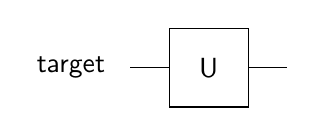
\begin{tikzpicture}[scale=.5] \node[draw=none] at (-3.5, 0) {target}; \draw (-2,0) -- (-1, 0); \draw (1, 0) -- (2, 0); \draw (-1,-1)--(-1,1)--(1,1)--(1,-1)--cycle; \node[draw=none] at (0, 0) {U}; \end{tikzpicture} } \]


\begin{DoxyParams}[1]{Parameters}
\mbox{\tt in,out}  & {\em multi\+Qubit} & object representing the set of all qubits \\
\hline
\mbox{\tt in}  & {\em target\+Qubit} & qubit to operate on \\
\hline
\mbox{\tt in}  & {\em alpha} & complex unitary parameter (row 1, column 1) \\
\hline
\mbox{\tt in}  & {\em beta} & complex unitary parameter (row 2, column 1) \\
\hline
\end{DoxyParams}

\begin{DoxyExceptions}{Exceptions}
{\em exit\+With\+Error} & if {\ttfamily target\+Qubit} is outside \mbox{[}0, {\ttfamily multi\+Qubit.\+num\+Qubits}), or if {\ttfamily alpha}, {\ttfamily beta} don\textquotesingle{}t satisfy $\vert${\ttfamily alpha$\vert$$^\wedge$2} + $\vert${\ttfamily beta$\vert$$^\wedge$2} = 1. \\
\hline
\end{DoxyExceptions}


Definition at line 100 of file Qu\+E\+S\+T\+\_\+env\+\_\+local.\+c.



References compact\+Unitary\+Local(), Multi\+Qubit\+::num\+Qubits, Qu\+E\+S\+T\+Assert(), and validate\+Alpha\+Beta().


\begin{DoxyCode}
101 \{
102     \mbox{\hyperlink{QuEST__env__local_8c_a3587b9d533e633ccf1abf9ad2ce45d8d}{QuESTAssert}}(targetQubit >= 0 && targetQubit < multiQubit.
      \mbox{\hyperlink{structMultiQubit_ab5b9795bdc6fb5855e1974dcbbaeb36f}{numQubits}}, 1, \_\_func\_\_);
103     \mbox{\hyperlink{QuEST__env__local_8c_a3587b9d533e633ccf1abf9ad2ce45d8d}{QuESTAssert}}(\mbox{\hyperlink{QuEST_8c_ae2b2c14a07dd7d50ff86032a3ca101d7}{validateAlphaBeta}}(alpha, beta), 6, \_\_func\_\_);
104 
105     \textcolor{comment}{// all values required to update state vector lie in this rank}
106     \mbox{\hyperlink{QuEST_8c_a9cee2d8716667a3318420a3b672f5b92}{compactUnitaryLocal}}(multiQubit, targetQubit, alpha, beta);
107 \}
\end{DoxyCode}
\mbox{\Hypertarget{QuEST__env__local_8c_ab4812953bc457405b3aa05a4c2f64f4a}\label{QuEST__env__local_8c_ab4812953bc457405b3aa05a4c2f64f4a}} 
\index{Qu\+E\+S\+T\+\_\+env\+\_\+local.\+c@{Qu\+E\+S\+T\+\_\+env\+\_\+local.\+c}!controlled\+Compact\+Unitary@{controlled\+Compact\+Unitary}}
\index{controlled\+Compact\+Unitary@{controlled\+Compact\+Unitary}!Qu\+E\+S\+T\+\_\+env\+\_\+local.\+c@{Qu\+E\+S\+T\+\_\+env\+\_\+local.\+c}}
\paragraph{\texorpdfstring{controlled\+Compact\+Unitary()}{controlledCompactUnitary()}}
{\footnotesize\ttfamily void controlled\+Compact\+Unitary (\begin{DoxyParamCaption}\item[{\mbox{\hyperlink{structMultiQubit}{Multi\+Qubit}}}]{multi\+Qubit,  }\item[{const int}]{control\+Qubit,  }\item[{const int}]{target\+Qubit,  }\item[{\mbox{\hyperlink{structComplex}{Complex}}}]{alpha,  }\item[{\mbox{\hyperlink{structComplex}{Complex}}}]{beta }\end{DoxyParamCaption})}



Apply a controlled unitary (single control, single target) parameterised by two given complex scalars. 

Given valid complex numbers $\alpha$ and $\beta$, applies the two-\/qubit unitary \[ \begin{pmatrix} 1 \\ & 1 \\ & & \alpha & -\beta^* \\ & & \beta & \alpha^* \end{pmatrix} \] to the control and target qubits. Valid $\alpha$, $\beta$ satisfy $|\alpha|^2 + |\beta|^2 = 1$. The target unitary is general up to a global phase factor. ~\newline
 \[ \setlength{\fboxrule}{0.01pt} \fbox{ 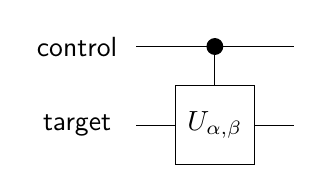
\begin{tikzpicture}[scale=.5] \node[draw=none] at (-3.5, 2) {control}; \node[draw=none] at (-3.5, 0) {target}; \draw (-2, 2) -- (2, 2); \draw[fill=black] (0, 2) circle (.2); \draw (0, 2) -- (0, 1); \draw (-2,0) -- (-1, 0); \draw (1, 0) -- (2, 0); \draw (-1,-1)--(-1,1)--(1,1)--(1,-1)--cycle; \node[draw=none] at (0, 0) {$U_{\alpha, \beta}$}; \end{tikzpicture} } \]


\begin{DoxyParams}[1]{Parameters}
\mbox{\tt in,out}  & {\em multi\+Qubit} & object representing the set of all qubits \\
\hline
\mbox{\tt in}  & {\em control\+Qubit} & apply the target unitary if this qubit has value 1 \\
\hline
\mbox{\tt in}  & {\em target\+Qubit} & qubit on which to apply the target unitary \\
\hline
\mbox{\tt in}  & {\em alpha} & complex unitary parameter (row 1, column 1) \\
\hline
\mbox{\tt in}  & {\em beta} & complex unitary parameter (row 2, column 1) \\
\hline
\end{DoxyParams}

\begin{DoxyExceptions}{Exceptions}
{\em exit\+With\+Error} & if either {\ttfamily control\+Qubit} or {\ttfamily target\+Qubit} are outside \mbox{[}0, {\ttfamily multi\+Qubit.\+num\+Qubits}) or are equal, or if {\ttfamily alpha}, {\ttfamily beta} don\textquotesingle{}t satisfy $\vert${\ttfamily alpha$\vert$$^\wedge$2} + $\vert${\ttfamily beta$\vert$$^\wedge$2} = 1. \\
\hline
\end{DoxyExceptions}


Definition at line 118 of file Qu\+E\+S\+T\+\_\+env\+\_\+local.\+c.



References controlled\+Compact\+Unitary\+Local(), Multi\+Qubit\+::num\+Qubits, Qu\+E\+S\+T\+Assert(), and validate\+Alpha\+Beta().


\begin{DoxyCode}
119 \{
120     \mbox{\hyperlink{QuEST__env__local_8c_a3587b9d533e633ccf1abf9ad2ce45d8d}{QuESTAssert}}(targetQubit >= 0 && targetQubit < multiQubit.
      \mbox{\hyperlink{structMultiQubit_ab5b9795bdc6fb5855e1974dcbbaeb36f}{numQubits}}, 1, \_\_func\_\_);
121     \mbox{\hyperlink{QuEST__env__local_8c_a3587b9d533e633ccf1abf9ad2ce45d8d}{QuESTAssert}}(controlQubit >= 0 && controlQubit < multiQubit.
      \mbox{\hyperlink{structMultiQubit_ab5b9795bdc6fb5855e1974dcbbaeb36f}{numQubits}}, 2, \_\_func\_\_);
122     \mbox{\hyperlink{QuEST__env__local_8c_a3587b9d533e633ccf1abf9ad2ce45d8d}{QuESTAssert}}(controlQubit != targetQubit, 3, \_\_func\_\_);
123     \mbox{\hyperlink{QuEST__env__local_8c_a3587b9d533e633ccf1abf9ad2ce45d8d}{QuESTAssert}}(\mbox{\hyperlink{QuEST_8c_ae2b2c14a07dd7d50ff86032a3ca101d7}{validateAlphaBeta}}(alpha, beta), 6, \_\_func\_\_);
124 
125 
126     \mbox{\hyperlink{QuEST_8c_afc77657651d52c47403b44b923a098a8}{controlledCompactUnitaryLocal}}(multiQubit, controlQubit, targetQubit, alpha
      , beta);
127 \}
\end{DoxyCode}
\mbox{\Hypertarget{QuEST__env__local_8c_a67576895bbc65463481a8ea24d9b1e22}\label{QuEST__env__local_8c_a67576895bbc65463481a8ea24d9b1e22}} 
\index{Qu\+E\+S\+T\+\_\+env\+\_\+local.\+c@{Qu\+E\+S\+T\+\_\+env\+\_\+local.\+c}!controlled\+Not@{controlled\+Not}}
\index{controlled\+Not@{controlled\+Not}!Qu\+E\+S\+T\+\_\+env\+\_\+local.\+c@{Qu\+E\+S\+T\+\_\+env\+\_\+local.\+c}}
\paragraph{\texorpdfstring{controlled\+Not()}{controlledNot()}}
{\footnotesize\ttfamily void controlled\+Not (\begin{DoxyParamCaption}\item[{\mbox{\hyperlink{structMultiQubit}{Multi\+Qubit}}}]{multi\+Qubit,  }\item[{const int}]{control\+Qubit,  }\item[{const int}]{target\+Qubit }\end{DoxyParamCaption})}



Apply the controlled not (single control, single target) gate, also known as the c-\/X, c-\/sigma-\/X, c-\/\+Pauli-\/X and c-\/bit-\/flip gate. 

This applies sigmaX to the target qubit if the control qubit has value 1. This effects the two-\/qubit unitary \[ \begin{pmatrix} 1 \\ & 1 \\\ & & & 1 \\ & & 1 \end{pmatrix} \] on the control and target qubits.

\[ \setlength{\fboxrule}{0.01pt} \fbox{ 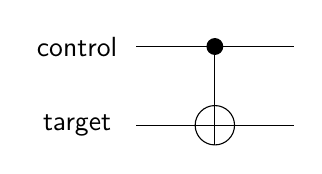
\begin{tikzpicture}[scale=.5] \node[draw=none] at (-3.5, 2) {control}; \node[draw=none] at (-3.5, 0) {target}; \draw (-2, 2) -- (2, 2); \draw[fill=black] (0, 2) circle (.2); \draw (0, 2) -- (0, -.5); \draw (-2,0) -- (2, 0); \draw (0, 0) circle (.5); \end{tikzpicture} } \] ~\newline
 
\begin{DoxyParams}[1]{Parameters}
\mbox{\tt in,out}  & {\em multi\+Qubit} & object representing the set of all qubits \\
\hline
\mbox{\tt in}  & {\em control\+Qubit} & nots the target if this qubit is 1 \\
\hline
\mbox{\tt in}  & {\em target\+Qubit} & qubit to not \\
\hline
\end{DoxyParams}

\begin{DoxyExceptions}{Exceptions}
{\em exit\+With\+Error} & if either {\ttfamily control\+Qubit} or {\ttfamily target\+Qubit} are outside \mbox{[}0, {\ttfamily multi\+Qubit.\+num\+Qubits}), or are equal. \\
\hline
\end{DoxyExceptions}


Definition at line 177 of file Qu\+E\+S\+T\+\_\+env\+\_\+local.\+c.



References controlled\+Not\+Local(), Multi\+Qubit\+::num\+Qubits, and Qu\+E\+S\+T\+Assert().


\begin{DoxyCode}
178 \{
179     \mbox{\hyperlink{QuEST__env__local_8c_a3587b9d533e633ccf1abf9ad2ce45d8d}{QuESTAssert}}(targetQubit >= 0 && targetQubit < multiQubit.
      \mbox{\hyperlink{structMultiQubit_ab5b9795bdc6fb5855e1974dcbbaeb36f}{numQubits}}, 1, \_\_func\_\_);
180     \mbox{\hyperlink{QuEST__env__local_8c_a3587b9d533e633ccf1abf9ad2ce45d8d}{QuESTAssert}}(controlQubit >= 0 && controlQubit < multiQubit.
      \mbox{\hyperlink{structMultiQubit_ab5b9795bdc6fb5855e1974dcbbaeb36f}{numQubits}}, 2, \_\_func\_\_);
181     \mbox{\hyperlink{QuEST__env__local_8c_a3587b9d533e633ccf1abf9ad2ce45d8d}{QuESTAssert}}(controlQubit != targetQubit, 3, \_\_func\_\_);
182     \mbox{\hyperlink{QuEST_8c_ad357a43e80e3baf013975b1b70942f4c}{controlledNotLocal}}(multiQubit, controlQubit, targetQubit);
183 \}
\end{DoxyCode}
\mbox{\Hypertarget{QuEST__env__local_8c_a8a701526263392599aa21d0d0f05d9d8}\label{QuEST__env__local_8c_a8a701526263392599aa21d0d0f05d9d8}} 
\index{Qu\+E\+S\+T\+\_\+env\+\_\+local.\+c@{Qu\+E\+S\+T\+\_\+env\+\_\+local.\+c}!controlled\+Unitary@{controlled\+Unitary}}
\index{controlled\+Unitary@{controlled\+Unitary}!Qu\+E\+S\+T\+\_\+env\+\_\+local.\+c@{Qu\+E\+S\+T\+\_\+env\+\_\+local.\+c}}
\paragraph{\texorpdfstring{controlled\+Unitary()}{controlledUnitary()}}
{\footnotesize\ttfamily void controlled\+Unitary (\begin{DoxyParamCaption}\item[{\mbox{\hyperlink{structMultiQubit}{Multi\+Qubit}}}]{multi\+Qubit,  }\item[{const int}]{control\+Qubit,  }\item[{const int}]{target\+Qubit,  }\item[{\mbox{\hyperlink{structComplexMatrix2}{Complex\+Matrix2}}}]{u }\end{DoxyParamCaption})}



Apply a general controlled unitary (single control, single target), which can include a global phase factor. 

The given unitary is applied to the target qubit if the control qubit has value 1, effecting the two-\/qubit unitary \[ \begin{pmatrix} 1 \\ & 1 \\ & & u_{00} & u_{01}\\ & & u_{10} & u_{11} \end{pmatrix} \] on the control and target qubits.

\[ \setlength{\fboxrule}{0.01pt} \fbox{ 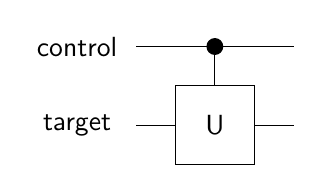
\begin{tikzpicture}[scale=.5] \node[draw=none] at (-3.5, 2) {control}; \node[draw=none] at (-3.5, 0) {target}; \draw (-2, 2) -- (2, 2); \draw[fill=black] (0, 2) circle (.2); \draw (0, 2) -- (0, 1); \draw (-2,0) -- (-1, 0); \draw (1, 0) -- (2, 0); \draw (-1,-1)--(-1,1)--(1,1)--(1,-1)--cycle; \node[draw=none] at (0, 0) {U}; \end{tikzpicture} } \]


\begin{DoxyParams}[1]{Parameters}
\mbox{\tt in,out}  & {\em multi\+Qubit} & object representing the set of all qubits \\
\hline
\mbox{\tt in}  & {\em control\+Qubit} & apply unitary if this qubit is 1 \\
\hline
\mbox{\tt in}  & {\em target\+Qubit} & qubit to operate on \\
\hline
\mbox{\tt in}  & {\em u} & single-\/qubit unitary matrix to apply \\
\hline
\end{DoxyParams}

\begin{DoxyExceptions}{Exceptions}
{\em exit\+With\+Error} & if either {\ttfamily control\+Qubit} or {\ttfamily target\+Qubit} are outside \mbox{[}0, {\ttfamily multi\+Qubit.\+num\+Qubits}) or are equal, or if {\ttfamily u} is not unitary. \\
\hline
\end{DoxyExceptions}


Definition at line 129 of file Qu\+E\+S\+T\+\_\+env\+\_\+local.\+c.



References controlled\+Unitary\+Local(), Multi\+Qubit\+::num\+Qubits, Qu\+E\+S\+T\+Assert(), and validate\+Matrix\+Is\+Unitary().


\begin{DoxyCode}
130 \{
131     \mbox{\hyperlink{QuEST__env__local_8c_a3587b9d533e633ccf1abf9ad2ce45d8d}{QuESTAssert}}(targetQubit >= 0 && targetQubit < multiQubit.
      \mbox{\hyperlink{structMultiQubit_ab5b9795bdc6fb5855e1974dcbbaeb36f}{numQubits}}, 1, \_\_func\_\_);
132     \mbox{\hyperlink{QuEST__env__local_8c_a3587b9d533e633ccf1abf9ad2ce45d8d}{QuESTAssert}}(controlQubit >= 0 && controlQubit < multiQubit.
      \mbox{\hyperlink{structMultiQubit_ab5b9795bdc6fb5855e1974dcbbaeb36f}{numQubits}}, 2, \_\_func\_\_);
133     \mbox{\hyperlink{QuEST__env__local_8c_a3587b9d533e633ccf1abf9ad2ce45d8d}{QuESTAssert}}(controlQubit != targetQubit, 3, \_\_func\_\_);
134     \mbox{\hyperlink{QuEST__env__local_8c_a3587b9d533e633ccf1abf9ad2ce45d8d}{QuESTAssert}}(\mbox{\hyperlink{QuEST_8c_ae4fea133d1a8f09ff8da03038100adb2}{validateMatrixIsUnitary}}(u), 5, \_\_func\_\_);
135 
136     \mbox{\hyperlink{QuEST_8c_a8a4afcff70195a306c082b8ed8d4e09a}{controlledUnitaryLocal}}(multiQubit, controlQubit, targetQubit, u);
137 \}
\end{DoxyCode}
\mbox{\Hypertarget{QuEST__env__local_8c_ae5f9019826f35e8b51b1716cfe397b45}\label{QuEST__env__local_8c_ae5f9019826f35e8b51b1716cfe397b45}} 
\index{Qu\+E\+S\+T\+\_\+env\+\_\+local.\+c@{Qu\+E\+S\+T\+\_\+env\+\_\+local.\+c}!exit\+With\+Error@{exit\+With\+Error}}
\index{exit\+With\+Error@{exit\+With\+Error}!Qu\+E\+S\+T\+\_\+env\+\_\+local.\+c@{Qu\+E\+S\+T\+\_\+env\+\_\+local.\+c}}
\paragraph{\texorpdfstring{exit\+With\+Error()}{exitWithError()}}
{\footnotesize\ttfamily void exit\+With\+Error (\begin{DoxyParamCaption}\item[{int}]{error\+Code,  }\item[{const char $\ast$}]{func }\end{DoxyParamCaption})}



Definition at line 234 of file Qu\+E\+S\+T\+\_\+env\+\_\+local.\+c.



Referenced by Qu\+E\+S\+T\+Assert().


\begin{DoxyCode}
234                                                    \{
235     printf(\textcolor{stringliteral}{"!!!\(\backslash\)n"});
236     printf(\textcolor{stringliteral}{"QuEST Error in function %s: %s\(\backslash\)n"}, func, \mbox{\hyperlink{QuEST_8c_aac1637696885c75b73a1ecf381cea713}{errorCodes}}[errorCode]);
237     printf(\textcolor{stringliteral}{"!!!\(\backslash\)n"});
238     printf(\textcolor{stringliteral}{"exiting..\(\backslash\)n"});
239     exit(errorCode);
240 \}
\end{DoxyCode}
\mbox{\Hypertarget{QuEST__env__local_8c_ad315c941a51bc053d39ebfa2040fd32e}\label{QuEST__env__local_8c_ad315c941a51bc053d39ebfa2040fd32e}} 
\index{Qu\+E\+S\+T\+\_\+env\+\_\+local.\+c@{Qu\+E\+S\+T\+\_\+env\+\_\+local.\+c}!find\+Probability\+Of\+Outcome@{find\+Probability\+Of\+Outcome}}
\index{find\+Probability\+Of\+Outcome@{find\+Probability\+Of\+Outcome}!Qu\+E\+S\+T\+\_\+env\+\_\+local.\+c@{Qu\+E\+S\+T\+\_\+env\+\_\+local.\+c}}
\paragraph{\texorpdfstring{find\+Probability\+Of\+Outcome()}{findProbabilityOfOutcome()}}
{\footnotesize\ttfamily \mbox{\hyperlink{QuEST__precision_8h_a4b654506f18b8bfd61ad2a29a7e38c25}{R\+E\+AL}} find\+Probability\+Of\+Outcome (\begin{DoxyParamCaption}\item[{\mbox{\hyperlink{structMultiQubit}{Multi\+Qubit}}}]{multi\+Qubit,  }\item[{const int}]{measure\+Qubit,  }\item[{int}]{outcome }\end{DoxyParamCaption})}



Gives the probability of a specified qubit being measured in the given outcome (0 or 1). 

This performs no actual measurement and does not change the state of the qubits.


\begin{DoxyParams}[1]{Parameters}
\mbox{\tt in}  & {\em multi\+Qubit} & object representing the set of all qubits \\
\hline
\mbox{\tt in}  & {\em measure\+Qubit} & qubit to study \\
\hline
\mbox{\tt in}  & {\em outcome} & for which to find the probability of the qubit being measured in \\
\hline
\end{DoxyParams}
\begin{DoxyReturn}{Returns}
probability of qubit measure\+Qubit being measured in the given outcome 
\end{DoxyReturn}

\begin{DoxyExceptions}{Exceptions}
{\em exit\+With\+Error} & if {\ttfamily measure\+Qubit} is outside \mbox{[}0, {\ttfamily multi\+Qubit.\+num\+Qubits}), or if {\ttfamily outcome} is not in \{0, 1\}. \\
\hline
\end{DoxyExceptions}


Definition at line 185 of file Qu\+E\+S\+T\+\_\+env\+\_\+local.\+c.



References find\+Probability\+Of\+Zero\+Local(), Multi\+Qubit\+::num\+Qubits, Qu\+E\+S\+T\+Assert(), and R\+E\+AL.



Referenced by collapse\+To\+Outcome(), and measure\+With\+Stats().


\begin{DoxyCode}
186 \{
187     \mbox{\hyperlink{QuEST__env__local_8c_a3587b9d533e633ccf1abf9ad2ce45d8d}{QuESTAssert}}(measureQubit >= 0 && measureQubit < multiQubit.
      \mbox{\hyperlink{structMultiQubit_ab5b9795bdc6fb5855e1974dcbbaeb36f}{numQubits}}, 2, \_\_func\_\_);
188     \mbox{\hyperlink{QuEST__precision_8h_a4b654506f18b8bfd61ad2a29a7e38c25}{REAL}} stateProb=0;
189     stateProb = \mbox{\hyperlink{QuEST_8c_a7c02cd0e1b4eac19771a0525f023249e}{findProbabilityOfZeroLocal}}(multiQubit, measureQubit);
190     \textcolor{keywordflow}{if} (outcome==1) stateProb = 1.0 - stateProb;
191     \textcolor{keywordflow}{return} stateProb;
192 \}
\end{DoxyCode}
\mbox{\Hypertarget{QuEST__env__local_8c_a3615f76fd5f57008d9b74bbd10533dd0}\label{QuEST__env__local_8c_a3615f76fd5f57008d9b74bbd10533dd0}} 
\index{Qu\+E\+S\+T\+\_\+env\+\_\+local.\+c@{Qu\+E\+S\+T\+\_\+env\+\_\+local.\+c}!get\+Imag\+Amp\+El@{get\+Imag\+Amp\+El}}
\index{get\+Imag\+Amp\+El@{get\+Imag\+Amp\+El}!Qu\+E\+S\+T\+\_\+env\+\_\+local.\+c@{Qu\+E\+S\+T\+\_\+env\+\_\+local.\+c}}
\paragraph{\texorpdfstring{get\+Imag\+Amp\+El()}{getImagAmpEl()}}
{\footnotesize\ttfamily \mbox{\hyperlink{QuEST__precision_8h_a4b654506f18b8bfd61ad2a29a7e38c25}{R\+E\+AL}} get\+Imag\+Amp\+El (\begin{DoxyParamCaption}\item[{\mbox{\hyperlink{structMultiQubit}{Multi\+Qubit}}}]{multi\+Qubit,  }\item[{long long int}]{index }\end{DoxyParamCaption})}



Get the imaginary component of the complex probability amplitude at an index in the state vector. 

For debugging purposes.


\begin{DoxyParams}[1]{Parameters}
\mbox{\tt in}  & {\em multi\+Qubit} & object representing a set of qubits \\
\hline
\mbox{\tt in}  & {\em index} & index in state vector of probability amplitudes \\
\hline
\end{DoxyParams}
\begin{DoxyReturn}{Returns}
imaginary component at that index 
\end{DoxyReturn}

\begin{DoxyExceptions}{Exceptions}
{\em exit\+With\+Error} & if {\ttfamily index} is outside \mbox{[}0, $2^{N}$) where $N = $ {\ttfamily multi\+Qubit.\+num\+Qubits} \\
\hline
\end{DoxyExceptions}


Definition at line 96 of file Qu\+E\+S\+T\+\_\+env\+\_\+local.\+c.



References Complex\+Array\+::imag, and Multi\+Qubit\+::state\+Vec.


\begin{DoxyCode}
96                                                              \{
97     \textcolor{keywordflow}{return} multiQubit.\mbox{\hyperlink{structMultiQubit_a45483190d6b01ef6b2f98f2bec9ab94f}{stateVec}}.\mbox{\hyperlink{structComplexArray_a79dde47c7ae530c79cebfdf57b225968}{imag}}[index];
98 \}
\end{DoxyCode}
\mbox{\Hypertarget{QuEST__env__local_8c_a317b786f577fa6bc136ea7f0ee7330a7}\label{QuEST__env__local_8c_a317b786f577fa6bc136ea7f0ee7330a7}} 
\index{Qu\+E\+S\+T\+\_\+env\+\_\+local.\+c@{Qu\+E\+S\+T\+\_\+env\+\_\+local.\+c}!get\+Real\+Amp\+El@{get\+Real\+Amp\+El}}
\index{get\+Real\+Amp\+El@{get\+Real\+Amp\+El}!Qu\+E\+S\+T\+\_\+env\+\_\+local.\+c@{Qu\+E\+S\+T\+\_\+env\+\_\+local.\+c}}
\paragraph{\texorpdfstring{get\+Real\+Amp\+El()}{getRealAmpEl()}}
{\footnotesize\ttfamily \mbox{\hyperlink{QuEST__precision_8h_a4b654506f18b8bfd61ad2a29a7e38c25}{R\+E\+AL}} get\+Real\+Amp\+El (\begin{DoxyParamCaption}\item[{\mbox{\hyperlink{structMultiQubit}{Multi\+Qubit}}}]{multi\+Qubit,  }\item[{long long int}]{index }\end{DoxyParamCaption})}



Get the real component of the complex probability amplitude at an index in the state vector. 

For debugging purposes.


\begin{DoxyParams}[1]{Parameters}
\mbox{\tt in}  & {\em multi\+Qubit} & object representing a set of qubits \\
\hline
\mbox{\tt in}  & {\em index} & index in state vector of probability amplitudes \\
\hline
\end{DoxyParams}
\begin{DoxyReturn}{Returns}
real component at that index 
\end{DoxyReturn}

\begin{DoxyExceptions}{Exceptions}
{\em exit\+With\+Error} & if {\ttfamily index} is outside \mbox{[}0, $2^{N}$) where $N = $ {\ttfamily multi\+Qubit.\+num\+Qubits} \\
\hline
\end{DoxyExceptions}


Definition at line 92 of file Qu\+E\+S\+T\+\_\+env\+\_\+local.\+c.



References Complex\+Array\+::real, and Multi\+Qubit\+::state\+Vec.


\begin{DoxyCode}
92                                                              \{
93     \textcolor{keywordflow}{return} multiQubit.\mbox{\hyperlink{structMultiQubit_a45483190d6b01ef6b2f98f2bec9ab94f}{stateVec}}.\mbox{\hyperlink{structComplexArray_a4195cac6c784ea1b6271f1c7dba1548a}{real}}[index];
94 \}
\end{DoxyCode}
\mbox{\Hypertarget{QuEST__env__local_8c_aa09b5dd93de6df1384b8f2c0041749ab}\label{QuEST__env__local_8c_aa09b5dd93de6df1384b8f2c0041749ab}} 
\index{Qu\+E\+S\+T\+\_\+env\+\_\+local.\+c@{Qu\+E\+S\+T\+\_\+env\+\_\+local.\+c}!hadamard@{hadamard}}
\index{hadamard@{hadamard}!Qu\+E\+S\+T\+\_\+env\+\_\+local.\+c@{Qu\+E\+S\+T\+\_\+env\+\_\+local.\+c}}
\paragraph{\texorpdfstring{hadamard()}{hadamard()}}
{\footnotesize\ttfamily void hadamard (\begin{DoxyParamCaption}\item[{\mbox{\hyperlink{structMultiQubit}{Multi\+Qubit}}}]{multi\+Qubit,  }\item[{const int}]{target\+Qubit }\end{DoxyParamCaption})}



Apply the single-\/qubit Hadamard gate. 

This takes $|0\rangle$ to $|+\rangle$ and $|1\rangle$ to $|-\rangle$, and is equivalent to a rotation of $\pi$ around the x-\/axis then $\pi/2$ about the y-\/axis on the Bloch-\/sphere. I.\+e. \[ \frac{1}{\sqrt{2}} \begin{pmatrix} 1 & 1 \\ 1 & -1 \end{pmatrix} \] ~\newline
 \[ \setlength{\fboxrule}{0.01pt} \fbox{ 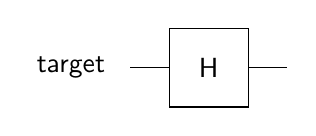
\begin{tikzpicture}[scale=.5] \node[draw=none] at (-3.5, 0) {target}; \draw (-2,0) -- (-1, 0); \draw (1, 0) -- (2, 0); \draw (-1,-1)--(-1,1)--(1,1)--(1,-1)--cycle; \node[draw=none] at (0, 0) {H}; \end{tikzpicture} } \] ~\newline
 
\begin{DoxyParams}[1]{Parameters}
\mbox{\tt in,out}  & {\em multi\+Qubit} & object representing the set of all qubits \\
\hline
\mbox{\tt in}  & {\em target\+Qubit} & qubit to operate on \\
\hline
\end{DoxyParams}

\begin{DoxyExceptions}{Exceptions}
{\em exit\+With\+Error} & if {\ttfamily target\+Qubit} is outside \mbox{[}0, {\ttfamily multi\+Qubit.\+num\+Qubits}). \\
\hline
\end{DoxyExceptions}


Definition at line 171 of file Qu\+E\+S\+T\+\_\+env\+\_\+local.\+c.



References hadamard\+Local(), Multi\+Qubit\+::num\+Qubits, and Qu\+E\+S\+T\+Assert().


\begin{DoxyCode}
172 \{
173     \mbox{\hyperlink{QuEST__env__local_8c_a3587b9d533e633ccf1abf9ad2ce45d8d}{QuESTAssert}}(targetQubit >= 0 && targetQubit < multiQubit.
      \mbox{\hyperlink{structMultiQubit_ab5b9795bdc6fb5855e1974dcbbaeb36f}{numQubits}}, 1, \_\_func\_\_);
174     \mbox{\hyperlink{QuEST_8c_aa9f0718b4dd794a3e1b143e3b153bfc5}{hadamardLocal}}(multiQubit, targetQubit);
175 \}
\end{DoxyCode}
\mbox{\Hypertarget{QuEST__env__local_8c_ad84a3ce68d1ca02b4e3f741ea45b6054}\label{QuEST__env__local_8c_ad84a3ce68d1ca02b4e3f741ea45b6054}} 
\index{Qu\+E\+S\+T\+\_\+env\+\_\+local.\+c@{Qu\+E\+S\+T\+\_\+env\+\_\+local.\+c}!init\+Qu\+E\+S\+T\+Env@{init\+Qu\+E\+S\+T\+Env}}
\index{init\+Qu\+E\+S\+T\+Env@{init\+Qu\+E\+S\+T\+Env}!Qu\+E\+S\+T\+\_\+env\+\_\+local.\+c@{Qu\+E\+S\+T\+\_\+env\+\_\+local.\+c}}
\paragraph{\texorpdfstring{init\+Qu\+E\+S\+T\+Env()}{initQuESTEnv()}}
{\footnotesize\ttfamily void init\+Qu\+E\+S\+T\+Env (\begin{DoxyParamCaption}\item[{\mbox{\hyperlink{structQuESTEnv}{Qu\+E\+S\+T\+Env}} $\ast$}]{env }\end{DoxyParamCaption})}



Initialize the Qu\+E\+ST environment. 

If something needs to be done to set up the execution environment, such as initializing M\+PI when running in distributed mode, it is handled here


\begin{DoxyParams}[1]{Parameters}
\mbox{\tt in,out}  & {\em env} & object representing the execution environment. A single instance is used for each program \\
\hline
\end{DoxyParams}


Definition at line 24 of file Qu\+E\+S\+T\+\_\+env\+\_\+local.\+c.



References Qu\+E\+S\+T\+Env\+::num\+Ranks, Qu\+E\+S\+T\+Seed\+Random\+Default(), and Qu\+E\+S\+T\+Env\+::rank.


\begin{DoxyCode}
24                                 \{
25     \textcolor{comment}{// init MPI environment}
26     env->\mbox{\hyperlink{structQuESTEnv_aa648bb336cf8598467cb62db00b9cee8}{rank}}=0;
27     env->\mbox{\hyperlink{structQuESTEnv_af22aacd7c9905accae28484785c193b4}{numRanks}}=1;
28         
29         \mbox{\hyperlink{QuEST_8c_a30b2a5228b8a21419db8aa82fa5e3167}{QuESTSeedRandomDefault}}();
30 \}
\end{DoxyCode}
\mbox{\Hypertarget{QuEST__env__local_8c_ad5774247d836267175c664cd0e451bcb}\label{QuEST__env__local_8c_ad5774247d836267175c664cd0e451bcb}} 
\index{Qu\+E\+S\+T\+\_\+env\+\_\+local.\+c@{Qu\+E\+S\+T\+\_\+env\+\_\+local.\+c}!measure@{measure}}
\index{measure@{measure}!Qu\+E\+S\+T\+\_\+env\+\_\+local.\+c@{Qu\+E\+S\+T\+\_\+env\+\_\+local.\+c}}
\paragraph{\texorpdfstring{measure()}{measure()}}
{\footnotesize\ttfamily int measure (\begin{DoxyParamCaption}\item[{\mbox{\hyperlink{structMultiQubit}{Multi\+Qubit}}}]{multi\+Qubit,  }\item[{int}]{measure\+Qubit }\end{DoxyParamCaption})}



Measures a single qubit, collapsing it randomly to 0 or 1. 

Outcome probabilities are weighted by the state vector, which is irreversibly changed after collapse to be consistent with the outcome.


\begin{DoxyParams}[1]{Parameters}
\mbox{\tt in,out}  & {\em multi\+Qubit} & object representing the set of all qubits \\
\hline
\mbox{\tt in}  & {\em measure\+Qubit} & qubit to measure \\
\hline
\end{DoxyParams}
\begin{DoxyReturn}{Returns}
the measurement outcome, 0 or 1 
\end{DoxyReturn}

\begin{DoxyExceptions}{Exceptions}
{\em exit\+With\+Error} & if {\ttfamily measure\+Qubit} is outside \mbox{[}0, {\ttfamily multi\+Qubit.\+num\+Qubits}) \\
\hline
\end{DoxyExceptions}


Definition at line 205 of file Qu\+E\+S\+T\+\_\+env\+\_\+local.\+c.



References measure\+With\+Stats(), Multi\+Qubit\+::num\+Qubits, Qu\+E\+S\+T\+Assert(), and R\+E\+AL.


\begin{DoxyCode}
205                                                     \{
206     \mbox{\hyperlink{QuEST__env__local_8c_a3587b9d533e633ccf1abf9ad2ce45d8d}{QuESTAssert}}(measureQubit >= 0 && measureQubit < multiQubit.
      \mbox{\hyperlink{structMultiQubit_ab5b9795bdc6fb5855e1974dcbbaeb36f}{numQubits}}, 2, \_\_func\_\_);
207     \mbox{\hyperlink{QuEST__precision_8h_a4b654506f18b8bfd61ad2a29a7e38c25}{REAL}} stateProb;
208     \textcolor{keywordflow}{return} \mbox{\hyperlink{QuEST__env__local_8c_a2ac46e470c750bf93c754e06c64b0a7a}{measureWithStats}}(multiQubit, measureQubit, &stateProb);
209 \}
\end{DoxyCode}
\mbox{\Hypertarget{QuEST__env__local_8c_a2ac46e470c750bf93c754e06c64b0a7a}\label{QuEST__env__local_8c_a2ac46e470c750bf93c754e06c64b0a7a}} 
\index{Qu\+E\+S\+T\+\_\+env\+\_\+local.\+c@{Qu\+E\+S\+T\+\_\+env\+\_\+local.\+c}!measure\+With\+Stats@{measure\+With\+Stats}}
\index{measure\+With\+Stats@{measure\+With\+Stats}!Qu\+E\+S\+T\+\_\+env\+\_\+local.\+c@{Qu\+E\+S\+T\+\_\+env\+\_\+local.\+c}}
\paragraph{\texorpdfstring{measure\+With\+Stats()}{measureWithStats()}}
{\footnotesize\ttfamily int measure\+With\+Stats (\begin{DoxyParamCaption}\item[{\mbox{\hyperlink{structMultiQubit}{Multi\+Qubit}}}]{multi\+Qubit,  }\item[{int}]{measure\+Qubit,  }\item[{\mbox{\hyperlink{QuEST__precision_8h_a4b654506f18b8bfd61ad2a29a7e38c25}{R\+E\+AL}} $\ast$}]{state\+Prob }\end{DoxyParamCaption})}



Measures a single qubit, collapsing it randomly to 0 or 1, and additionally gives the probability of that outcome. 

Outcome probabilities are weighted by the state vector, which is irreversibly changed after collapse to be consistent with the outcome.


\begin{DoxyParams}[1]{Parameters}
\mbox{\tt in,out}  & {\em multi\+Qubit} & object representing the set of all qubits \\
\hline
\mbox{\tt in}  & {\em measure\+Qubit} & qubit to measure \\
\hline
\mbox{\tt out}  & {\em state\+Prob} & a pointer to a R\+E\+AL which is set to the probability of the occurred outcome \\
\hline
\end{DoxyParams}
\begin{DoxyReturn}{Returns}
the measurement outcome, 0 or 1 
\end{DoxyReturn}

\begin{DoxyExceptions}{Exceptions}
{\em exit\+With\+Error} & if {\ttfamily measure\+Qubit} is outside \mbox{[}0, {\ttfamily multi\+Qubit.\+num\+Qubits}) \\
\hline
\end{DoxyExceptions}


Definition at line 211 of file Qu\+E\+S\+T\+\_\+env\+\_\+local.\+c.



References collapse\+To\+Outcome\+Local(), find\+Probability\+Of\+Outcome(), genrand\+\_\+real1(), Multi\+Qubit\+::num\+Qubits, Qu\+E\+S\+T\+Assert(), R\+E\+AL, and R\+E\+A\+L\+\_\+\+E\+PS.



Referenced by measure().


\begin{DoxyCode}
211                                                                               \{
212     \mbox{\hyperlink{QuEST__env__local_8c_a3587b9d533e633ccf1abf9ad2ce45d8d}{QuESTAssert}}(measureQubit >= 0 && measureQubit < multiQubit.
      \mbox{\hyperlink{structMultiQubit_ab5b9795bdc6fb5855e1974dcbbaeb36f}{numQubits}}, 2, \_\_func\_\_);
213 
214     \textcolor{keywordtype}{int} outcome;
215     \textcolor{comment}{// find probability of qubit being in state 1}
216     \mbox{\hyperlink{QuEST__precision_8h_a4b654506f18b8bfd61ad2a29a7e38c25}{REAL}} stateProbInternal = \mbox{\hyperlink{QuEST__env__local_8c_ad315c941a51bc053d39ebfa2040fd32e}{findProbabilityOfOutcome}}(multiQubit, measureQubit,
       1);
217 
218     \textcolor{comment}{// we can't collapse to a state that has a probability too close to zero}
219     \textcolor{keywordflow}{if} (stateProbInternal<\mbox{\hyperlink{QuEST__precision_8h_aebb5e6716e06431296af4d1a71744dec}{REAL\_EPS}}) outcome=0;
220     \textcolor{keywordflow}{else} \textcolor{keywordflow}{if} (1-stateProbInternal<\mbox{\hyperlink{QuEST__precision_8h_aebb5e6716e06431296af4d1a71744dec}{REAL\_EPS}}) outcome=1;
221     \textcolor{keywordflow}{else} \{
222         \textcolor{comment}{// ok. both P(0) and P(1) are large enough to resolve}
223         \textcolor{comment}{// generate random float on [0,1]}
224         \textcolor{keywordtype}{float} randNum = \mbox{\hyperlink{mt19937ar_8c_ac94ab75771800274ed1a2bedeca86f04}{genrand\_real1}}();
225         \textcolor{keywordflow}{if} (randNum<=stateProbInternal) outcome = 1;
226         \textcolor{keywordflow}{else} outcome = 0;
227     \} 
228     \textcolor{keywordflow}{if} (outcome==0) stateProbInternal = 1-stateProbInternal;
229     \mbox{\hyperlink{QuEST_8c_a01d9a8b7ff0e09ec399e158389783aa9}{collapseToOutcomeLocal}}(multiQubit, measureQubit, stateProbInternal, outcome);
230     *stateProb = stateProbInternal;
231     \textcolor{keywordflow}{return} outcome;
232 \}
\end{DoxyCode}
\mbox{\Hypertarget{QuEST__env__local_8c_ae395a79690283ed81106afadd7a8cd8a}\label{QuEST__env__local_8c_ae395a79690283ed81106afadd7a8cd8a}} 
\index{Qu\+E\+S\+T\+\_\+env\+\_\+local.\+c@{Qu\+E\+S\+T\+\_\+env\+\_\+local.\+c}!multi\+Controlled\+Unitary@{multi\+Controlled\+Unitary}}
\index{multi\+Controlled\+Unitary@{multi\+Controlled\+Unitary}!Qu\+E\+S\+T\+\_\+env\+\_\+local.\+c@{Qu\+E\+S\+T\+\_\+env\+\_\+local.\+c}}
\paragraph{\texorpdfstring{multi\+Controlled\+Unitary()}{multiControlledUnitary()}}
{\footnotesize\ttfamily void multi\+Controlled\+Unitary (\begin{DoxyParamCaption}\item[{\mbox{\hyperlink{structMultiQubit}{Multi\+Qubit}}}]{multi\+Qubit,  }\item[{int $\ast$}]{control\+Qubits,  }\item[{const int}]{num\+Control\+Qubits,  }\item[{const int}]{target\+Qubit,  }\item[{\mbox{\hyperlink{structComplexMatrix2}{Complex\+Matrix2}}}]{u }\end{DoxyParamCaption})}



Apply a general multiple-\/control single-\/target unitary, which can include a global phase factor. 

Any number of control qubits can be specified, and if all have value 1, the given unitary is applied to the target qubit. This effects the many-\/qubit unitary \[ \begin{pmatrix} 1 \\ & 1 \\\ & & \ddots \\ & & & u_{00} & u_{01}\\ & & & u_{10} & u_{11} \end{pmatrix} \] on the control and target qubits. The given 2x2 Complex\+Matrix must be unitary, otherwise an error is thrown.

\[ \setlength{\fboxrule}{0.01pt} \fbox{ 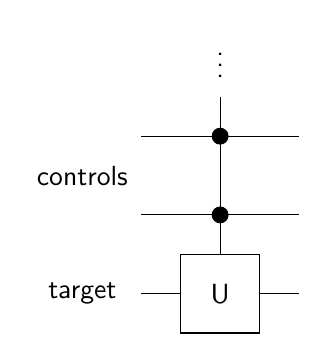
\begin{tikzpicture}[scale=.5] \node[draw=none] at (-3.5, 3) {controls}; \node[draw=none] at (-3.5, 0) {target}; \node[draw=none] at (0, 6) {$\vdots$}; \draw (0, 5) -- (0, 4); \draw (-2, 4) -- (2, 4); \draw[fill=black] (0, 4) circle (.2); \draw (0, 4) -- (0, 2); \draw (-2, 2) -- (2, 2); \draw[fill=black] (0, 2) circle (.2); \draw (0, 2) -- (0, 1); \draw (-2,0) -- (-1, 0); \draw (1, 0) -- (2, 0); \draw (-1,-1)--(-1,1)--(1,1)--(1,-1)--cycle; \node[draw=none] at (0, 0) {U}; \end{tikzpicture} } \]


\begin{DoxyParams}[1]{Parameters}
\mbox{\tt in,out}  & {\em multi\+Qubit} & object representing the set of all qubits \\
\hline
\mbox{\tt in}  & {\em control\+Qubits} & applies unitary if all qubits in this array equal 1 \\
\hline
\mbox{\tt in}  & {\em num\+Control\+Qubits} & number of control qubits \\
\hline
\mbox{\tt in}  & {\em target\+Qubit} & qubit to operate on \\
\hline
\mbox{\tt in}  & {\em u} & single-\/qubit unitary matrix to apply \\
\hline
\end{DoxyParams}

\begin{DoxyExceptions}{Exceptions}
{\em exit\+With\+Error} & if {\ttfamily num\+Control\+Qubits} is outside \mbox{[}1, {\ttfamily multi\+Qubit.\+num\+Qubits}\mbox{]}), or if any qubit index ({\ttfamily target\+Qubit} or one in {\ttfamily control\+Qubits}) is outside \mbox{[}0, {\ttfamily multi\+Qubit.\+num\+Qubits}\mbox{]}), or if {\ttfamily control\+Qubits} contains {\ttfamily target\+Qubit}, or if {\ttfamily u} is not unitary. \\
\hline
\end{DoxyExceptions}


Definition at line 139 of file Qu\+E\+S\+T\+\_\+env\+\_\+local.\+c.



References multi\+Controlled\+Unitary\+Local(), Multi\+Qubit\+::num\+Qubits, Qu\+E\+S\+T\+Assert(), and validate\+Matrix\+Is\+Unitary().


\begin{DoxyCode}
140 \{
141     \mbox{\hyperlink{QuEST__env__local_8c_a3587b9d533e633ccf1abf9ad2ce45d8d}{QuESTAssert}}(targetQubit >= 0 && targetQubit < multiQubit.
      \mbox{\hyperlink{structMultiQubit_ab5b9795bdc6fb5855e1974dcbbaeb36f}{numQubits}}, 1, \_\_func\_\_);
142     \mbox{\hyperlink{QuEST__env__local_8c_a3587b9d533e633ccf1abf9ad2ce45d8d}{QuESTAssert}}(numControlQubits > 0 && numControlQubits <= multiQubit.
      \mbox{\hyperlink{structMultiQubit_ab5b9795bdc6fb5855e1974dcbbaeb36f}{numQubits}}, 4, \_\_func\_\_);
143     \mbox{\hyperlink{QuEST__env__local_8c_a3587b9d533e633ccf1abf9ad2ce45d8d}{QuESTAssert}}(\mbox{\hyperlink{QuEST_8c_ae4fea133d1a8f09ff8da03038100adb2}{validateMatrixIsUnitary}}(u), 5, \_\_func\_\_);
144 
145     \textcolor{keywordtype}{long} \textcolor{keywordtype}{long} \textcolor{keywordtype}{int} mask=0; 
146     \textcolor{keywordflow}{for} (\textcolor{keywordtype}{int} i=0; i<numControlQubits; i++) mask = mask | (1LL<<controlQubits[i]);
147     \mbox{\hyperlink{QuEST__env__local_8c_a3587b9d533e633ccf1abf9ad2ce45d8d}{QuESTAssert}}(mask >=0 && mask <= (1LL<<multiQubit.\mbox{\hyperlink{structMultiQubit_ab5b9795bdc6fb5855e1974dcbbaeb36f}{numQubits}})-1, 2, \_\_func\_\_);
148     \mbox{\hyperlink{QuEST__env__local_8c_a3587b9d533e633ccf1abf9ad2ce45d8d}{QuESTAssert}}((mask & (1LL<<targetQubit)) != (1LL<<targetQubit), 3, \_\_func\_\_);
149 
150     \mbox{\hyperlink{QuEST_8c_a1309eabcba3cb97fbc3cd2e606d17766}{multiControlledUnitaryLocal}}(multiQubit, targetQubit, mask, u);
151 \}
\end{DoxyCode}
\mbox{\Hypertarget{QuEST__env__local_8c_aae7a8a7f1ccbddb7f76b6c52b746bb43}\label{QuEST__env__local_8c_aae7a8a7f1ccbddb7f76b6c52b746bb43}} 
\index{Qu\+E\+S\+T\+\_\+env\+\_\+local.\+c@{Qu\+E\+S\+T\+\_\+env\+\_\+local.\+c}!phase\+Gate@{phase\+Gate}}
\index{phase\+Gate@{phase\+Gate}!Qu\+E\+S\+T\+\_\+env\+\_\+local.\+c@{Qu\+E\+S\+T\+\_\+env\+\_\+local.\+c}}
\paragraph{\texorpdfstring{phase\+Gate()}{phaseGate()}}
{\footnotesize\ttfamily void phase\+Gate (\begin{DoxyParamCaption}\item[{\mbox{\hyperlink{structMultiQubit}{Multi\+Qubit}}}]{multi\+Qubit,  }\item[{const int}]{target\+Qubit,  }\item[{enum \mbox{\hyperlink{QuEST_8h_a5739021c733cecc49647956b2f7338ea}{phase\+Gate\+Type}}}]{type }\end{DoxyParamCaption})}



Definition at line 165 of file Qu\+E\+S\+T\+\_\+env\+\_\+local.\+c.



Referenced by s\+Gate(), sigma\+Z(), and t\+Gate().


\begin{DoxyCode}
166 \{
167     \mbox{\hyperlink{QuEST__env__local_8c_a3587b9d533e633ccf1abf9ad2ce45d8d}{QuESTAssert}}(targetQubit >= 0 && targetQubit < multiQubit.
      \mbox{\hyperlink{structMultiQubit_ab5b9795bdc6fb5855e1974dcbbaeb36f}{numQubits}}, 1, \_\_func\_\_);
168     \mbox{\hyperlink{QuEST_8c_a3a54566b73ac84c312d7da4f56ffbc3b}{phaseGateLocal}}(multiQubit, targetQubit, type);
169 \}
\end{DoxyCode}
\mbox{\Hypertarget{QuEST__env__local_8c_a3587b9d533e633ccf1abf9ad2ce45d8d}\label{QuEST__env__local_8c_a3587b9d533e633ccf1abf9ad2ce45d8d}} 
\index{Qu\+E\+S\+T\+\_\+env\+\_\+local.\+c@{Qu\+E\+S\+T\+\_\+env\+\_\+local.\+c}!Qu\+E\+S\+T\+Assert@{Qu\+E\+S\+T\+Assert}}
\index{Qu\+E\+S\+T\+Assert@{Qu\+E\+S\+T\+Assert}!Qu\+E\+S\+T\+\_\+env\+\_\+local.\+c@{Qu\+E\+S\+T\+\_\+env\+\_\+local.\+c}}
\paragraph{\texorpdfstring{Qu\+E\+S\+T\+Assert()}{QuESTAssert()}}
{\footnotesize\ttfamily void Qu\+E\+S\+T\+Assert (\begin{DoxyParamCaption}\item[{int}]{is\+Valid,  }\item[{int}]{error\+Code,  }\item[{const char $\ast$}]{func }\end{DoxyParamCaption})}



Definition at line 242 of file Qu\+E\+S\+T\+\_\+env\+\_\+local.\+c.



Referenced by collapse\+To\+Outcome(), compact\+Unitary(), controlled\+Compact\+Unitary(), controlled\+Not(), controlled\+Phase\+Gate(), controlled\+Unitary(), create\+Multi\+Qubit(), find\+Probability\+Of\+Outcome(), hadamard(), initialize\+State\+From\+Single\+File(), measure(), measure\+With\+Stats(), multi\+Controlled\+Phase\+Gate(), multi\+Controlled\+Unitary(), phase\+Gate(), report\+State(), sigma\+X(), sigma\+Y(), and unitary().


\begin{DoxyCode}
242                                                               \{
243     \textcolor{keywordflow}{if} (!isValid) \mbox{\hyperlink{QuEST__env__local_8c_ae5f9019826f35e8b51b1716cfe397b45}{exitWithError}}(errorCode, func);
244 \}
\end{DoxyCode}
\mbox{\Hypertarget{QuEST__env__local_8c_a62da5b58d8ce84e6f4d24be1b872294e}\label{QuEST__env__local_8c_a62da5b58d8ce84e6f4d24be1b872294e}} 
\index{Qu\+E\+S\+T\+\_\+env\+\_\+local.\+c@{Qu\+E\+S\+T\+\_\+env\+\_\+local.\+c}!report\+Node\+List@{report\+Node\+List}}
\index{report\+Node\+List@{report\+Node\+List}!Qu\+E\+S\+T\+\_\+env\+\_\+local.\+c@{Qu\+E\+S\+T\+\_\+env\+\_\+local.\+c}}
\paragraph{\texorpdfstring{report\+Node\+List()}{reportNodeList()}}
{\footnotesize\ttfamily void report\+Node\+List (\begin{DoxyParamCaption}\item[{\mbox{\hyperlink{structQuESTEnv}{Qu\+E\+S\+T\+Env}}}]{env }\end{DoxyParamCaption})}



Report a list of C\+PU hostnames and the rank that is running on each if running with M\+PI enabled and an error message otherwise. 

For debugging purposes. 
\begin{DoxyParams}[1]{Parameters}
\mbox{\tt in}  & {\em env} & object representing the execution environment. A single instance is used for each program \\
\hline
\end{DoxyParams}


Definition at line 58 of file Qu\+E\+S\+T\+\_\+env\+\_\+local.\+c.


\begin{DoxyCode}
58                                  \{
59     printf(\textcolor{stringliteral}{"Hostname unknown: running locally\(\backslash\)n"});
60 \}
\end{DoxyCode}
\mbox{\Hypertarget{QuEST__env__local_8c_af8a14ae79c3fb2c0b5f6255cc37bebf9}\label{QuEST__env__local_8c_af8a14ae79c3fb2c0b5f6255cc37bebf9}} 
\index{Qu\+E\+S\+T\+\_\+env\+\_\+local.\+c@{Qu\+E\+S\+T\+\_\+env\+\_\+local.\+c}!report\+Qu\+E\+S\+T\+Env@{report\+Qu\+E\+S\+T\+Env}}
\index{report\+Qu\+E\+S\+T\+Env@{report\+Qu\+E\+S\+T\+Env}!Qu\+E\+S\+T\+\_\+env\+\_\+local.\+c@{Qu\+E\+S\+T\+\_\+env\+\_\+local.\+c}}
\paragraph{\texorpdfstring{report\+Qu\+E\+S\+T\+Env()}{reportQuESTEnv()}}
{\footnotesize\ttfamily void report\+Qu\+E\+S\+T\+Env (\begin{DoxyParamCaption}\item[{\mbox{\hyperlink{structQuESTEnv}{Qu\+E\+S\+T\+Env}}}]{env }\end{DoxyParamCaption})}



Report information about the Qu\+E\+ST environment. 


\begin{DoxyParams}[1]{Parameters}
\mbox{\tt in}  & {\em env} & object representing the execution environment. A single instance is used for each program \\
\hline
\end{DoxyParams}


Definition at line 45 of file Qu\+E\+S\+T\+\_\+env\+\_\+local.\+c.



References Qu\+E\+S\+T\+Env\+::num\+Ranks, and R\+E\+AL.


\begin{DoxyCode}
45                                  \{
46     printf(\textcolor{stringliteral}{"EXECUTION ENVIRONMENT:\(\backslash\)n"});
47     printf(\textcolor{stringliteral}{"Running locally on one node\(\backslash\)n"});
48     printf(\textcolor{stringliteral}{"Number of ranks is %d\(\backslash\)n"}, env.\mbox{\hyperlink{structQuESTEnv_af22aacd7c9905accae28484785c193b4}{numRanks}});
49 \textcolor{preprocessor}{# ifdef \_OPENMP}
50     printf(\textcolor{stringliteral}{"OpenMP enabled\(\backslash\)n"});
51     printf(\textcolor{stringliteral}{"Number of threads available is %d\(\backslash\)n"}, omp\_get\_max\_threads());
52 \textcolor{preprocessor}{# else}
53     printf(\textcolor{stringliteral}{"OpenMP disabled\(\backslash\)n"});
54 \textcolor{preprocessor}{# endif}
55     printf(\textcolor{stringliteral}{"Precision: size of REAL is %ld bytes\(\backslash\)n"}, \textcolor{keyword}{sizeof}(\mbox{\hyperlink{QuEST__precision_8h_a4b654506f18b8bfd61ad2a29a7e38c25}{REAL}}));
56 \}
\end{DoxyCode}
\mbox{\Hypertarget{QuEST__env__local_8c_a86e396e06b7d527cac20ba0108872423}\label{QuEST__env__local_8c_a86e396e06b7d527cac20ba0108872423}} 
\index{Qu\+E\+S\+T\+\_\+env\+\_\+local.\+c@{Qu\+E\+S\+T\+\_\+env\+\_\+local.\+c}!sigmaX@{sigmaX}}
\index{sigmaX@{sigmaX}!Qu\+E\+S\+T\+\_\+env\+\_\+local.\+c@{Qu\+E\+S\+T\+\_\+env\+\_\+local.\+c}}
\paragraph{\texorpdfstring{sigma\+X()}{sigmaX()}}
{\footnotesize\ttfamily void sigmaX (\begin{DoxyParamCaption}\item[{\mbox{\hyperlink{structMultiQubit}{Multi\+Qubit}}}]{multi\+Qubit,  }\item[{const int}]{target\+Qubit }\end{DoxyParamCaption})}



Apply the single-\/qubit sigma-\/X (also known as the X, Pauli-\/X, N\+OT or bit-\/flip) gate. 

This is a rotation of $\pi$ around the x-\/axis on the Bloch sphere. I.\+e. \[ \begin{pmatrix} 0 & 1 \\ 1 & 0 \end{pmatrix} \] ~\newline
 \[ \setlength{\fboxrule}{0.01pt} \fbox{ 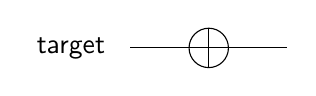
\begin{tikzpicture}[scale=.5] \node[draw=none] at (-3.5, 0) {target}; \draw (-2,0) -- (2, 0); \draw (0, 0) circle (.5); \draw (0, .5) -- (0, -.5); \end{tikzpicture} } \] ~\newline
 
\begin{DoxyParams}[1]{Parameters}
\mbox{\tt in,out}  & {\em multi\+Qubit} & object representing the set of all qubits \\
\hline
\mbox{\tt in}  & {\em target\+Qubit} & qubit to operate on \\
\hline
\end{DoxyParams}

\begin{DoxyExceptions}{Exceptions}
{\em exit\+With\+Error} & if {\ttfamily target\+Qubit} is outside \mbox{[}0, {\ttfamily multi\+Qubit.\+num\+Qubits}). \\
\hline
\end{DoxyExceptions}


Definition at line 153 of file Qu\+E\+S\+T\+\_\+env\+\_\+local.\+c.



References Multi\+Qubit\+::num\+Qubits, Qu\+E\+S\+T\+Assert(), and sigma\+X\+Local().


\begin{DoxyCode}
154 \{
155     \mbox{\hyperlink{QuEST__env__local_8c_a3587b9d533e633ccf1abf9ad2ce45d8d}{QuESTAssert}}(targetQubit >= 0 && targetQubit < multiQubit.
      \mbox{\hyperlink{structMultiQubit_ab5b9795bdc6fb5855e1974dcbbaeb36f}{numQubits}}, 1, \_\_func\_\_);
156     \mbox{\hyperlink{QuEST_8c_a74822fd86bb5d81766e6e8dbdcd62df1}{sigmaXLocal}}(multiQubit, targetQubit);
157 \}
\end{DoxyCode}
\mbox{\Hypertarget{QuEST__env__local_8c_a1f54d70a42403f7e1c2e2c2007332f61}\label{QuEST__env__local_8c_a1f54d70a42403f7e1c2e2c2007332f61}} 
\index{Qu\+E\+S\+T\+\_\+env\+\_\+local.\+c@{Qu\+E\+S\+T\+\_\+env\+\_\+local.\+c}!sigmaY@{sigmaY}}
\index{sigmaY@{sigmaY}!Qu\+E\+S\+T\+\_\+env\+\_\+local.\+c@{Qu\+E\+S\+T\+\_\+env\+\_\+local.\+c}}
\paragraph{\texorpdfstring{sigma\+Y()}{sigmaY()}}
{\footnotesize\ttfamily void sigmaY (\begin{DoxyParamCaption}\item[{\mbox{\hyperlink{structMultiQubit}{Multi\+Qubit}}}]{multi\+Qubit,  }\item[{const int}]{target\+Qubit }\end{DoxyParamCaption})}



Apply the single-\/qubit sigma-\/Y (also known as the Y or Pauli-\/Y) gate. 

This is a rotation of $\pi$ around the Y-\/axis on the Bloch sphere. I.\+e. \[ \begin{pmatrix} 0 & -i \\ i & 0 \end{pmatrix} \] ~\newline
 \[ \setlength{\fboxrule}{0.01pt} \fbox{ \begin{tikzpicture}[scale=.5] \node[draw=none] at (-3.5, 0) {target}; \draw (-2,0) -- (-1, 0); \draw (1, 0) -- (2, 0); \draw (-1,-1)--(-1,1)--(1,1)--(1,-1)--cycle; \node[draw=none] at (0, 0) {$\sigma_y$}; \end{tikzpicture} } \] ~\newline
 
\begin{DoxyParams}[1]{Parameters}
\mbox{\tt in,out}  & {\em multi\+Qubit} & object representing the set of all qubits \\
\hline
\mbox{\tt in}  & {\em target\+Qubit} & qubit to operate on \\
\hline
\end{DoxyParams}

\begin{DoxyExceptions}{Exceptions}
{\em exit\+With\+Error} & if {\ttfamily target\+Qubit} is outside \mbox{[}0, {\ttfamily multi\+Qubit.\+num\+Qubits}). \\
\hline
\end{DoxyExceptions}


Definition at line 159 of file Qu\+E\+S\+T\+\_\+env\+\_\+local.\+c.



References Multi\+Qubit\+::num\+Qubits, Qu\+E\+S\+T\+Assert(), and sigma\+Y\+Local().


\begin{DoxyCode}
160 \{
161     \mbox{\hyperlink{QuEST__env__local_8c_a3587b9d533e633ccf1abf9ad2ce45d8d}{QuESTAssert}}(targetQubit >= 0 && targetQubit < multiQubit.
      \mbox{\hyperlink{structMultiQubit_ab5b9795bdc6fb5855e1974dcbbaeb36f}{numQubits}}, 1, \_\_func\_\_);
162     \mbox{\hyperlink{QuEST_8c_a81fbfaed65a742a7dfd622e17652245e}{sigmaYLocal}}(multiQubit, targetQubit);
163 \}
\end{DoxyCode}
\mbox{\Hypertarget{QuEST__env__local_8c_a8d31fe2d1ad4d01e2a1f5f6b8bc15b77}\label{QuEST__env__local_8c_a8d31fe2d1ad4d01e2a1f5f6b8bc15b77}} 
\index{Qu\+E\+S\+T\+\_\+env\+\_\+local.\+c@{Qu\+E\+S\+T\+\_\+env\+\_\+local.\+c}!sync\+Qu\+E\+S\+T\+Env@{sync\+Qu\+E\+S\+T\+Env}}
\index{sync\+Qu\+E\+S\+T\+Env@{sync\+Qu\+E\+S\+T\+Env}!Qu\+E\+S\+T\+\_\+env\+\_\+local.\+c@{Qu\+E\+S\+T\+\_\+env\+\_\+local.\+c}}
\paragraph{\texorpdfstring{sync\+Qu\+E\+S\+T\+Env()}{syncQuESTEnv()}}
{\footnotesize\ttfamily void sync\+Qu\+E\+S\+T\+Env (\begin{DoxyParamCaption}\item[{\mbox{\hyperlink{structQuESTEnv}{Qu\+E\+S\+T\+Env}}}]{env }\end{DoxyParamCaption})}



Guarantees that all code up to the given point has been executed on all nodes (if running in distributed mode) 


\begin{DoxyParams}[1]{Parameters}
\mbox{\tt in}  & {\em env} & object representing the execution environment. A single instance is used for each program \\
\hline
\end{DoxyParams}


Definition at line 33 of file Qu\+E\+S\+T\+\_\+env\+\_\+local.\+c.


\begin{DoxyCode}
33                                \{
34     \textcolor{comment}{// MPI Barrier goes here in MPI version. }
35 \} 
\end{DoxyCode}
\mbox{\Hypertarget{QuEST__env__local_8c_ac7e38d768a1bd79019f88cc1e6295092}\label{QuEST__env__local_8c_ac7e38d768a1bd79019f88cc1e6295092}} 
\index{Qu\+E\+S\+T\+\_\+env\+\_\+local.\+c@{Qu\+E\+S\+T\+\_\+env\+\_\+local.\+c}!sync\+Qu\+E\+S\+T\+Success@{sync\+Qu\+E\+S\+T\+Success}}
\index{sync\+Qu\+E\+S\+T\+Success@{sync\+Qu\+E\+S\+T\+Success}!Qu\+E\+S\+T\+\_\+env\+\_\+local.\+c@{Qu\+E\+S\+T\+\_\+env\+\_\+local.\+c}}
\paragraph{\texorpdfstring{sync\+Qu\+E\+S\+T\+Success()}{syncQuESTSuccess()}}
{\footnotesize\ttfamily int sync\+Qu\+E\+S\+T\+Success (\begin{DoxyParamCaption}\item[{int}]{success\+Code }\end{DoxyParamCaption})}



Performs a logical A\+ND on all success\+Codes held by all processes. 

If any one process has a zero success\+Code all processes will return a zero success code.


\begin{DoxyParams}[1]{Parameters}
\mbox{\tt in}  & {\em env} & object representing the execution environment. A single instance is used for each program \\
\hline
\mbox{\tt in}  & {\em success\+Code} & 1 if process task succeeded, 0 if process task failed \\
\hline
\end{DoxyParams}
\begin{DoxyReturn}{Returns}
1 if all processes succeeded, 0 if any one process failed 
\end{DoxyReturn}


Definition at line 37 of file Qu\+E\+S\+T\+\_\+env\+\_\+local.\+c.


\begin{DoxyCode}
37                                      \{
38     \textcolor{keywordflow}{return} successCode;
39 \}
\end{DoxyCode}
\mbox{\Hypertarget{QuEST__env__local_8c_a7a0877e33700f6bad48adb51b7b3fb67}\label{QuEST__env__local_8c_a7a0877e33700f6bad48adb51b7b3fb67}} 
\index{Qu\+E\+S\+T\+\_\+env\+\_\+local.\+c@{Qu\+E\+S\+T\+\_\+env\+\_\+local.\+c}!unitary@{unitary}}
\index{unitary@{unitary}!Qu\+E\+S\+T\+\_\+env\+\_\+local.\+c@{Qu\+E\+S\+T\+\_\+env\+\_\+local.\+c}}
\paragraph{\texorpdfstring{unitary()}{unitary()}}
{\footnotesize\ttfamily void unitary (\begin{DoxyParamCaption}\item[{\mbox{\hyperlink{structMultiQubit}{Multi\+Qubit}}}]{multi\+Qubit,  }\item[{const int}]{target\+Qubit,  }\item[{\mbox{\hyperlink{structComplexMatrix2}{Complex\+Matrix2}}}]{u }\end{DoxyParamCaption})}



Apply a general single-\/qubit unitary (including a global phase factor). 

The passed 2x2 Complex\+Matrix must be unitary, otherwise an error is thrown.

\[ \setlength{\fboxrule}{0.01pt} \fbox{ \begin{tikzpicture}[scale=.5] \node[draw=none] at (-3.5, 0) {target}; \draw (-2,0) -- (-1, 0); \draw (1, 0) -- (2, 0); \draw (-1,-1)--(-1,1)--(1,1)--(1,-1)--cycle; \node[draw=none] at (0, 0) {U}; \end{tikzpicture} } \]


\begin{DoxyParams}[1]{Parameters}
\mbox{\tt in,out}  & {\em multi\+Qubit} & object representing the set of all qubits \\
\hline
\mbox{\tt in}  & {\em target\+Qubit} & qubit to operate on \\
\hline
\mbox{\tt in}  & {\em u} & unitary matrix to apply \\
\hline
\end{DoxyParams}

\begin{DoxyExceptions}{Exceptions}
{\em exit\+With\+Error} & if {\ttfamily target\+Qubit} is outside \mbox{[}0, {\ttfamily multi\+Qubit.\+num\+Qubits}), or matrix {\ttfamily u} is not unitary. \\
\hline
\end{DoxyExceptions}


Definition at line 109 of file Qu\+E\+S\+T\+\_\+env\+\_\+local.\+c.



References Multi\+Qubit\+::num\+Qubits, Qu\+E\+S\+T\+Assert(), unitary\+Local(), and validate\+Matrix\+Is\+Unitary().


\begin{DoxyCode}
110 \{
111     \mbox{\hyperlink{QuEST__env__local_8c_a3587b9d533e633ccf1abf9ad2ce45d8d}{QuESTAssert}}(targetQubit >= 0 && targetQubit < multiQubit.
      \mbox{\hyperlink{structMultiQubit_ab5b9795bdc6fb5855e1974dcbbaeb36f}{numQubits}}, 1, \_\_func\_\_);
112     \mbox{\hyperlink{QuEST__env__local_8c_a3587b9d533e633ccf1abf9ad2ce45d8d}{QuESTAssert}}(\mbox{\hyperlink{QuEST_8c_ae4fea133d1a8f09ff8da03038100adb2}{validateMatrixIsUnitary}}(u), 5, \_\_func\_\_);
113 
114     \textcolor{comment}{// all values required to update state vector lie in this rank}
115     \mbox{\hyperlink{QuEST_8c_ac134fb45b0a7248c5d15e16eb7139a35}{unitaryLocal}}(multiQubit, targetQubit, u);
116 \}
\end{DoxyCode}

\hypertarget{QuEST__env__localGPU_8cu}{}\subsection{Qu\+E\+S\+T\+\_\+env\+\_\+local\+G\+P\+U.\+cu File Reference}
\label{QuEST__env__localGPU_8cu}\index{Qu\+E\+S\+T\+\_\+env\+\_\+local\+G\+P\+U.\+cu@{Qu\+E\+S\+T\+\_\+env\+\_\+local\+G\+P\+U.\+cu}}


An implementation of the A\+PI in qubits.\+h for a local (non-\/\+M\+PI) environment.  


{\ttfamily \#include \char`\"{}../\+Qu\+E\+S\+T.\+h\char`\"{}}\newline
{\ttfamily \#include \char`\"{}../\+Qu\+E\+S\+T\+\_\+precision.\+h\char`\"{}}\newline
{\ttfamily \#include \char`\"{}../mt19937ar.\+h\char`\"{}}\newline
{\ttfamily \#include \char`\"{}Qu\+E\+S\+T\+\_\+internal.\+h\char`\"{}}\newline
{\ttfamily \#include $<$stdlib.\+h$>$}\newline
{\ttfamily \#include $<$stdio.\+h$>$}\newline
{\ttfamily \#include $<$math.\+h$>$}\newline
\subsubsection*{Macros}
\begin{DoxyCompactItemize}
\item 
\#define \mbox{\hyperlink{QuEST__env__localGPU_8cu_ad72dbcf6d0153db1b8d8a58001feed83}{D\+E\+B\+UG}}~0
\item 
\#define \mbox{\hyperlink{QuEST__env__localGPU_8cu_aa57d77a0903e334e963c66ddc5ed3f53}{R\+E\+D\+U\+C\+E\+\_\+\+S\+H\+A\+R\+E\+D\+\_\+\+S\+I\+ZE}}~512
\end{DoxyCompactItemize}
\subsubsection*{Functions}
\begin{DoxyCompactItemize}
\item 
\mbox{\hyperlink{QuEST__precision_8h_a4b654506f18b8bfd61ad2a29a7e38c25}{R\+E\+AL}} \mbox{\hyperlink{QuEST__env__localGPU_8cu_a818a4c7cd7252d2b10b896b12fa431d3}{calc\+Total\+Probability}} (\mbox{\hyperlink{structMultiQubit}{Multi\+Qubit}} multi\+Qubit)
\begin{DoxyCompactList}\small\item\em Calculate the probability of being in any state by taking the norm of the entire state vector. \end{DoxyCompactList}\item 
void \mbox{\hyperlink{QuEST__env__localGPU_8cu_abd4bc926cd3f9b65610bb228d0c59fe0}{close\+Qu\+E\+S\+T\+Env}} (\mbox{\hyperlink{structQuESTEnv}{Qu\+E\+S\+T\+Env}} \mbox{\hyperlink{runTests_8c_a5fd8ba97fcae3408ae6221dfc3cc1f93}{env}})
\begin{DoxyCompactList}\small\item\em Close Qu\+E\+ST environment. \end{DoxyCompactList}\item 
\mbox{\hyperlink{QuEST__precision_8h_a4b654506f18b8bfd61ad2a29a7e38c25}{R\+E\+AL}} \mbox{\hyperlink{QuEST__env__localGPU_8cu_a07418ebac70fd9ae5d051d089961631d}{collapse\+To\+Outcome}} (\mbox{\hyperlink{structMultiQubit}{Multi\+Qubit}} multi\+Qubit, const int measure\+Qubit, int outcome)
\begin{DoxyCompactList}\small\item\em Updates the state vector to be consistent with measuring the measure qubit in the given outcome (0 or 1), and returns the probability of such a measurement outcome. \end{DoxyCompactList}\item 
\+\_\+\+\_\+global\+\_\+\+\_\+ void \mbox{\hyperlink{QuEST__env__localGPU_8cu_ab9c5c19b3bd2ac5d1ac4506fa21c1c84}{collapse\+To\+Outcome\+Kernel}} (\mbox{\hyperlink{structMultiQubit}{Multi\+Qubit}} multi\+Qubit, int measure\+Qubit, \mbox{\hyperlink{QuEST__precision_8h_a4b654506f18b8bfd61ad2a29a7e38c25}{R\+E\+AL}} total\+Probability, int outcome)
\item 
void \mbox{\hyperlink{QuEST__env__localGPU_8cu_a03b13dfcabd8c59b50dbdd3af44ba8b2}{compact\+Unitary}} (\mbox{\hyperlink{structMultiQubit}{Multi\+Qubit}} multi\+Qubit, const int target\+Qubit, \mbox{\hyperlink{structComplex}{Complex}} alpha, \mbox{\hyperlink{structComplex}{Complex}} beta)
\begin{DoxyCompactList}\small\item\em Apply a single-\/qubit unitary parameterised by two given complex scalars. \end{DoxyCompactList}\item 
\+\_\+\+\_\+global\+\_\+\+\_\+ void \mbox{\hyperlink{QuEST__env__localGPU_8cu_aec6ec83ed63a7848ddb8f16c88846d25}{compact\+Unitary\+Kernel}} (\mbox{\hyperlink{structMultiQubit}{Multi\+Qubit}} multi\+Qubit, const int rot\+Qubit, \mbox{\hyperlink{structComplex}{Complex}} alpha, \mbox{\hyperlink{structComplex}{Complex}} beta)
\item 
int \mbox{\hyperlink{QuEST__env__localGPU_8cu_a793584932ae384c82e7e42db7d35d18d}{compare\+States}} (\mbox{\hyperlink{structMultiQubit}{Multi\+Qubit}} mq1, \mbox{\hyperlink{structMultiQubit}{Multi\+Qubit}} mq2, \mbox{\hyperlink{QuEST__precision_8h_a4b654506f18b8bfd61ad2a29a7e38c25}{R\+E\+AL}} precision)
\begin{DoxyCompactList}\small\item\em Return whether two given wavefunctions are equivalent within a given precision Global phase included in equivalence check. \end{DoxyCompactList}\item 
void \mbox{\hyperlink{QuEST__env__localGPU_8cu_ab4812953bc457405b3aa05a4c2f64f4a}{controlled\+Compact\+Unitary}} (\mbox{\hyperlink{structMultiQubit}{Multi\+Qubit}} multi\+Qubit, const int control\+Qubit, const int target\+Qubit, \mbox{\hyperlink{structComplex}{Complex}} alpha, \mbox{\hyperlink{structComplex}{Complex}} beta)
\begin{DoxyCompactList}\small\item\em Apply a controlled unitary (single control, single target) parameterised by two given complex scalars. \end{DoxyCompactList}\item 
\+\_\+\+\_\+global\+\_\+\+\_\+ void \mbox{\hyperlink{QuEST__env__localGPU_8cu_ac9af28ce6412c545805c6275ad7636d5}{controlled\+Compact\+Unitary\+Kernel}} (\mbox{\hyperlink{structMultiQubit}{Multi\+Qubit}} multi\+Qubit, const int control\+Qubit, const int target\+Qubit, \mbox{\hyperlink{structComplex}{Complex}} alpha, \mbox{\hyperlink{structComplex}{Complex}} beta)
\item 
void \mbox{\hyperlink{QuEST__env__localGPU_8cu_a67576895bbc65463481a8ea24d9b1e22}{controlled\+Not}} (\mbox{\hyperlink{structMultiQubit}{Multi\+Qubit}} multi\+Qubit, const int control\+Qubit, const int target\+Qubit)
\begin{DoxyCompactList}\small\item\em Apply the controlled not (single control, single target) gate, also known as the c-\/X, c-\/sigma-\/X, c-\/\+Pauli-\/X and c-\/bit-\/flip gate. \end{DoxyCompactList}\item 
\+\_\+\+\_\+global\+\_\+\+\_\+ void \mbox{\hyperlink{QuEST__env__localGPU_8cu_a625723cfbffdde3b3b312f8573d530a3}{controlled\+Not\+Kernel}} (\mbox{\hyperlink{structMultiQubit}{Multi\+Qubit}} multi\+Qubit, const int control\+Qubit, const int target\+Qubit)
\item 
void \mbox{\hyperlink{QuEST__env__localGPU_8cu_a11a96159191cbf1b01a1080e7f045aac}{controlled\+Phase\+Gate}} (\mbox{\hyperlink{structMultiQubit}{Multi\+Qubit}} multi\+Qubit, const int id\+Qubit1, const int id\+Qubit2)
\begin{DoxyCompactList}\small\item\em Apply the (two-\/qubit) controlled phase gate, also known as the controlled sigmaZ gate. \end{DoxyCompactList}\item 
\+\_\+\+\_\+global\+\_\+\+\_\+ void \mbox{\hyperlink{QuEST__env__localGPU_8cu_a67313a10fc0760b39a5ce9ef1d505830}{controlled\+Phase\+Gate\+Kernel}} (\mbox{\hyperlink{structMultiQubit}{Multi\+Qubit}} multi\+Qubit, const int id\+Qubit1, const int id\+Qubit2)
\item 
void \mbox{\hyperlink{QuEST__env__localGPU_8cu_a8a701526263392599aa21d0d0f05d9d8}{controlled\+Unitary}} (\mbox{\hyperlink{structMultiQubit}{Multi\+Qubit}} multi\+Qubit, const int control\+Qubit, const int target\+Qubit, \mbox{\hyperlink{structComplexMatrix2}{Complex\+Matrix2}} u)
\begin{DoxyCompactList}\small\item\em Apply a general controlled unitary (single control, single target), which can include a global phase factor. \end{DoxyCompactList}\item 
\+\_\+\+\_\+global\+\_\+\+\_\+ void \mbox{\hyperlink{QuEST__env__localGPU_8cu_a8e75679cf6d66e11507ee227ab584473}{controlled\+Unitary\+Kernel}} (\mbox{\hyperlink{structMultiQubit}{Multi\+Qubit}} multi\+Qubit, const int control\+Qubit, const int target\+Qubit, \mbox{\hyperlink{structComplexMatrix2}{Complex\+Matrix2}} u)
\item 
\+\_\+\+\_\+global\+\_\+\+\_\+ void \mbox{\hyperlink{QuEST__env__localGPU_8cu_a250e9d66ad94ed2682e76a3c7502c8e1}{copy\+Shared\+Reduce\+Block}} (\mbox{\hyperlink{QuEST__precision_8h_a4b654506f18b8bfd61ad2a29a7e38c25}{R\+E\+AL}} $\ast$array\+In, \mbox{\hyperlink{QuEST__precision_8h_a4b654506f18b8bfd61ad2a29a7e38c25}{R\+E\+AL}} $\ast$reduced\+Array, int length)
\item 
void \mbox{\hyperlink{QuEST__env__localGPU_8cu_a0d255fec1e375244d4cb980fac92621d}{copy\+State\+From\+G\+PU}} (\mbox{\hyperlink{structMultiQubit}{Multi\+Qubit}} multi\+Qubit)
\item 
void \mbox{\hyperlink{QuEST__env__localGPU_8cu_a5b8880e65a521b4f6445af21b68d88ef}{copy\+State\+To\+G\+PU}} (\mbox{\hyperlink{structMultiQubit}{Multi\+Qubit}} multi\+Qubit)
\item 
void \mbox{\hyperlink{QuEST__env__localGPU_8cu_a9c02591bc64c2918503afa231d90d83f}{create\+Multi\+Qubit}} (\mbox{\hyperlink{structMultiQubit}{Multi\+Qubit}} $\ast$multi\+Qubit, int num\+Qubits, \mbox{\hyperlink{structQuESTEnv}{Qu\+E\+S\+T\+Env}} \mbox{\hyperlink{runTests_8c_a5fd8ba97fcae3408ae6221dfc3cc1f93}{env}})
\begin{DoxyCompactList}\small\item\em Create a \mbox{\hyperlink{structMultiQubit}{Multi\+Qubit}} object representing a set of qubits. \end{DoxyCompactList}\item 
void \mbox{\hyperlink{QuEST__env__localGPU_8cu_ae5d6acc322314d7a3d8a2eccf00d3b19}{destroy\+Multi\+Qubit}} (\mbox{\hyperlink{structMultiQubit}{Multi\+Qubit}} multi\+Qubit, \mbox{\hyperlink{structQuESTEnv}{Qu\+E\+S\+T\+Env}} \mbox{\hyperlink{runTests_8c_a5fd8ba97fcae3408ae6221dfc3cc1f93}{env}})
\begin{DoxyCompactList}\small\item\em Deallocate a \mbox{\hyperlink{structMultiQubit}{Multi\+Qubit}} object representing a set of qubits. \end{DoxyCompactList}\item 
void \mbox{\hyperlink{QuEST__env__localGPU_8cu_ae5f9019826f35e8b51b1716cfe397b45}{exit\+With\+Error}} (int error\+Code, const char $\ast$func)
\item 
static \+\_\+\+\_\+device\+\_\+\+\_\+ int \mbox{\hyperlink{QuEST__env__localGPU_8cu_a6ffa51987d8ad8f6c0fc07fd3492277f}{extract\+Bit}} (int location\+Of\+Bit\+From\+Right, long long int the\+Encoded\+Number)
\item 
\mbox{\hyperlink{QuEST__precision_8h_a4b654506f18b8bfd61ad2a29a7e38c25}{R\+E\+AL}} \mbox{\hyperlink{QuEST__env__localGPU_8cu_ad315c941a51bc053d39ebfa2040fd32e}{find\+Probability\+Of\+Outcome}} (\mbox{\hyperlink{structMultiQubit}{Multi\+Qubit}} multi\+Qubit, const int measure\+Qubit, int outcome)
\begin{DoxyCompactList}\small\item\em Gives the probability of a specified qubit being measured in the given outcome (0 or 1). \end{DoxyCompactList}\item 
\mbox{\hyperlink{QuEST__precision_8h_a4b654506f18b8bfd61ad2a29a7e38c25}{R\+E\+AL}} \mbox{\hyperlink{QuEST__env__localGPU_8cu_a2e4cedb70bd181d250b3abb945cc108e}{find\+Probability\+Of\+Zero}} (\mbox{\hyperlink{structMultiQubit}{Multi\+Qubit}} multi\+Qubit, const int measure\+Qubit)
\begin{DoxyCompactList}\small\item\em Measure the probability of a specified qubit being in the zero state. \end{DoxyCompactList}\item 
\+\_\+\+\_\+global\+\_\+\+\_\+ void \mbox{\hyperlink{QuEST__env__localGPU_8cu_aa9d9643aec790baf66e6322e591ebfd6}{find\+Probability\+Of\+Zero\+Kernel}} (\mbox{\hyperlink{structMultiQubit}{Multi\+Qubit}} multi\+Qubit, const int measure\+Qubit, \mbox{\hyperlink{QuEST__precision_8h_a4b654506f18b8bfd61ad2a29a7e38c25}{R\+E\+AL}} $\ast$reduced\+Array)
\item 
void \mbox{\hyperlink{QuEST__env__localGPU_8cu_a8f10aabf9f607f19093aee54630caa21}{get\+Environment\+String}} (\mbox{\hyperlink{structQuESTEnv}{Qu\+E\+S\+T\+Env}} \mbox{\hyperlink{runTests_8c_a5fd8ba97fcae3408ae6221dfc3cc1f93}{env}}, \mbox{\hyperlink{structMultiQubit}{Multi\+Qubit}} multi\+Qubit, char str\mbox{[}200\mbox{]})
\item 
\mbox{\hyperlink{QuEST__precision_8h_a4b654506f18b8bfd61ad2a29a7e38c25}{R\+E\+AL}} \mbox{\hyperlink{QuEST__env__localGPU_8cu_a3615f76fd5f57008d9b74bbd10533dd0}{get\+Imag\+Amp\+El}} (\mbox{\hyperlink{structMultiQubit}{Multi\+Qubit}} multi\+Qubit, long long int index)
\begin{DoxyCompactList}\small\item\em Get the imaginary component of the complex probability amplitude at an index in the state vector. \end{DoxyCompactList}\item 
int \mbox{\hyperlink{QuEST__env__localGPU_8cu_a112c74b3365bda6697813d9931b55377}{get\+Num\+Reduction\+Levels}} (long long int num\+Values\+To\+Reduce, int num\+Reduced\+Per\+Level)
\item 
\mbox{\hyperlink{QuEST__precision_8h_a4b654506f18b8bfd61ad2a29a7e38c25}{R\+E\+AL}} \mbox{\hyperlink{QuEST__env__localGPU_8cu_a317b786f577fa6bc136ea7f0ee7330a7}{get\+Real\+Amp\+El}} (\mbox{\hyperlink{structMultiQubit}{Multi\+Qubit}} multi\+Qubit, long long int index)
\begin{DoxyCompactList}\small\item\em Get the real component of the complex probability amplitude at an index in the state vector. \end{DoxyCompactList}\item 
int \mbox{\hyperlink{QuEST__env__localGPU_8cu_a0aabd5ed69a74e5bc0b46a17af45c886}{G\+P\+U\+Exists}} (void)
\item 
void \mbox{\hyperlink{QuEST__env__localGPU_8cu_aa09b5dd93de6df1384b8f2c0041749ab}{hadamard}} (\mbox{\hyperlink{structMultiQubit}{Multi\+Qubit}} multi\+Qubit, const int target\+Qubit)
\begin{DoxyCompactList}\small\item\em Apply the single-\/qubit Hadamard gate. \end{DoxyCompactList}\item 
\+\_\+\+\_\+global\+\_\+\+\_\+ void \mbox{\hyperlink{QuEST__env__localGPU_8cu_aca19ea42f8ff8d21871394db3a7a2a2a}{hadamard\+Kernel}} (\mbox{\hyperlink{structMultiQubit}{Multi\+Qubit}} multi\+Qubit, const int target\+Qubit)
\item 
void \mbox{\hyperlink{QuEST__env__localGPU_8cu_ae1b983b41249836ed2c2a81f77d83c40}{init\+Classical\+State}} (\mbox{\hyperlink{structMultiQubit}{Multi\+Qubit}} multi\+Qubit, long long int state\+Ind)
\begin{DoxyCompactList}\small\item\em Initialise a set of $ N $ qubits to the classical state with index {\ttfamily state\+Ind}. \end{DoxyCompactList}\item 
void \+\_\+\+\_\+global\+\_\+\+\_\+ \mbox{\hyperlink{QuEST__env__localGPU_8cu_a5ffdb83d58185c1caf2ef0675d9c4ad6}{init\+Classical\+State\+Kernel}} (long long int state\+Vec\+Size, \mbox{\hyperlink{QuEST__precision_8h_a4b654506f18b8bfd61ad2a29a7e38c25}{R\+E\+AL}} $\ast$state\+Vec\+Real, \mbox{\hyperlink{QuEST__precision_8h_a4b654506f18b8bfd61ad2a29a7e38c25}{R\+E\+AL}} $\ast$state\+Vec\+Imag, long long int state\+Ind)
\item 
void \mbox{\hyperlink{QuEST__env__localGPU_8cu_a433876ee9f3bcc54af346300f571fc3c}{initialize\+State\+From\+Single\+File}} (\mbox{\hyperlink{structMultiQubit}{Multi\+Qubit}} $\ast$multi\+Qubit, char filename\mbox{[}200\mbox{]}, \mbox{\hyperlink{structQuESTEnv}{Qu\+E\+S\+T\+Env}} \mbox{\hyperlink{runTests_8c_a5fd8ba97fcae3408ae6221dfc3cc1f93}{env}})
\begin{DoxyCompactList}\small\item\em Initialises the wavefunction amplitudes according to those specified in a file. \end{DoxyCompactList}\item 
void \mbox{\hyperlink{QuEST__env__localGPU_8cu_ad84a3ce68d1ca02b4e3f741ea45b6054}{init\+Qu\+E\+S\+T\+Env}} (\mbox{\hyperlink{structQuESTEnv}{Qu\+E\+S\+T\+Env}} $\ast$\mbox{\hyperlink{runTests_8c_a5fd8ba97fcae3408ae6221dfc3cc1f93}{env}})
\begin{DoxyCompactList}\small\item\em Initialize the Qu\+E\+ST environment. \end{DoxyCompactList}\item 
void \mbox{\hyperlink{QuEST__env__localGPU_8cu_a4b737ff9b4267609ef27e6cb4c42dc68}{init\+State\+Debug}} (\mbox{\hyperlink{structMultiQubit}{Multi\+Qubit}} multi\+Qubit)
\begin{DoxyCompactList}\small\item\em Initialise the state vector of probability amplitudes to an (unphysical) state with each component of each probability amplitude a unique floating point value. \end{DoxyCompactList}\item 
void \+\_\+\+\_\+global\+\_\+\+\_\+ \mbox{\hyperlink{QuEST__env__localGPU_8cu_a2f83bb3e7c5408d3a19161e9f0be6e35}{init\+State\+Debug\+Kernel}} (long long int state\+Vec\+Size, \mbox{\hyperlink{QuEST__precision_8h_a4b654506f18b8bfd61ad2a29a7e38c25}{R\+E\+AL}} $\ast$state\+Vec\+Real, \mbox{\hyperlink{QuEST__precision_8h_a4b654506f18b8bfd61ad2a29a7e38c25}{R\+E\+AL}} $\ast$state\+Vec\+Imag)
\item 
void \mbox{\hyperlink{QuEST__env__localGPU_8cu_a7169fd0442cbc3418f3fac4d13363ca2}{init\+State\+Of\+Single\+Qubit}} (\mbox{\hyperlink{structMultiQubit}{Multi\+Qubit}} $\ast$multi\+Qubit, int qubit\+Id, int outcome)
\begin{DoxyCompactList}\small\item\em Initialise the state vector of probability amplitudes such that one qubit is set to \textquotesingle{}outcome\textquotesingle{} and all other qubits are in an equal superposition of zero and one. \end{DoxyCompactList}\item 
void \+\_\+\+\_\+global\+\_\+\+\_\+ \mbox{\hyperlink{QuEST__env__localGPU_8cu_a1eb51dd82f1cbbef94d3cb7d2ca73e28}{init\+State\+Of\+Single\+Qubit\+Kernel}} (long long int state\+Vec\+Size, \mbox{\hyperlink{QuEST__precision_8h_a4b654506f18b8bfd61ad2a29a7e38c25}{R\+E\+AL}} $\ast$state\+Vec\+Real, \mbox{\hyperlink{QuEST__precision_8h_a4b654506f18b8bfd61ad2a29a7e38c25}{R\+E\+AL}} $\ast$state\+Vec\+Imag, int qubit\+Id, int outcome)
\item 
void \mbox{\hyperlink{QuEST__env__localGPU_8cu_af8a0082e2f695145bbfbb572e4c2e4f1}{init\+State\+Plus}} (\mbox{\hyperlink{structMultiQubit}{Multi\+Qubit}} multi\+Qubit)
\begin{DoxyCompactList}\small\item\em Initialise a set of $ N $ qubits to the plus state $ {| + \rangle}^{\otimes N} = \frac{1}{\sqrt{2^N}} (| 0 \rangle + | 1 \rangle)^{\otimes N} $. \end{DoxyCompactList}\item 
void \+\_\+\+\_\+global\+\_\+\+\_\+ \mbox{\hyperlink{QuEST__env__localGPU_8cu_abddc47ea8fe014ed09dc82542bcbfe6f}{init\+State\+Plus\+Kernel}} (long long int state\+Vec\+Size, \mbox{\hyperlink{QuEST__precision_8h_a4b654506f18b8bfd61ad2a29a7e38c25}{R\+E\+AL}} $\ast$state\+Vec\+Real, \mbox{\hyperlink{QuEST__precision_8h_a4b654506f18b8bfd61ad2a29a7e38c25}{R\+E\+AL}} $\ast$state\+Vec\+Imag)
\item 
void \mbox{\hyperlink{QuEST__env__localGPU_8cu_a9ba8171c9ec5c42202b144026527e9ec}{init\+State\+Zero}} (\mbox{\hyperlink{structMultiQubit}{Multi\+Qubit}} multi\+Qubit)
\begin{DoxyCompactList}\small\item\em Initialise a set of $ N $ qubits to the classical zero state $ {| 0 \rangle}^{\otimes N} $. \end{DoxyCompactList}\item 
void \+\_\+\+\_\+global\+\_\+\+\_\+ \mbox{\hyperlink{QuEST__env__localGPU_8cu_aa6b649062c49c37ac93aac0d6be6eedd}{init\+State\+Zero\+Kernel}} (long long int state\+Vec\+Size, \mbox{\hyperlink{QuEST__precision_8h_a4b654506f18b8bfd61ad2a29a7e38c25}{R\+E\+AL}} $\ast$state\+Vec\+Real, \mbox{\hyperlink{QuEST__precision_8h_a4b654506f18b8bfd61ad2a29a7e38c25}{R\+E\+AL}} $\ast$state\+Vec\+Imag)
\item 
\+\_\+\+\_\+device\+\_\+\+\_\+ \+\_\+\+\_\+host\+\_\+\+\_\+ unsigned int \mbox{\hyperlink{QuEST__env__localGPU_8cu_a8ce1e311ea72b862a8757dc71082fbf3}{log2\+Int}} (unsigned int x)
\item 
int \mbox{\hyperlink{QuEST__env__localGPU_8cu_ad5774247d836267175c664cd0e451bcb}{measure}} (\mbox{\hyperlink{structMultiQubit}{Multi\+Qubit}} multi\+Qubit, int measure\+Qubit)
\begin{DoxyCompactList}\small\item\em Measures a single qubit, collapsing it randomly to 0 or 1. \end{DoxyCompactList}\item 
\mbox{\hyperlink{QuEST__precision_8h_a4b654506f18b8bfd61ad2a29a7e38c25}{R\+E\+AL}} \mbox{\hyperlink{QuEST__env__localGPU_8cu_a21094de735f3cb48488a184cfa4d8d41}{measure\+In\+Zero}} (\mbox{\hyperlink{structMultiQubit}{Multi\+Qubit}} multi\+Qubit, const int measure\+Qubit)
\begin{DoxyCompactList}\small\item\em Update the state vector to be consistent with measuring measure\+Qubit=0. \end{DoxyCompactList}\item 
\+\_\+\+\_\+global\+\_\+\+\_\+ void \mbox{\hyperlink{QuEST__env__localGPU_8cu_a8f87a4777c69c875fece83d4b5eb29ba}{measure\+In\+Zero\+Kernel}} (\mbox{\hyperlink{structMultiQubit}{Multi\+Qubit}} multi\+Qubit, int measure\+Qubit, \mbox{\hyperlink{QuEST__precision_8h_a4b654506f18b8bfd61ad2a29a7e38c25}{R\+E\+AL}} total\+Probability)
\item 
int \mbox{\hyperlink{QuEST__env__localGPU_8cu_a2ac46e470c750bf93c754e06c64b0a7a}{measure\+With\+Stats}} (\mbox{\hyperlink{structMultiQubit}{Multi\+Qubit}} multi\+Qubit, int measure\+Qubit, \mbox{\hyperlink{QuEST__precision_8h_a4b654506f18b8bfd61ad2a29a7e38c25}{R\+E\+AL}} $\ast$state\+Prob)
\begin{DoxyCompactList}\small\item\em Measures a single qubit, collapsing it randomly to 0 or 1, and additionally gives the probability of that outcome. \end{DoxyCompactList}\item 
void \mbox{\hyperlink{QuEST__env__localGPU_8cu_afc1835c6b43b6e59ce7df7b13f274fc7}{multi\+Controlled\+Phase\+Gate}} (\mbox{\hyperlink{structMultiQubit}{Multi\+Qubit}} multi\+Qubit, int $\ast$control\+Qubits, int num\+Control\+Qubits)
\begin{DoxyCompactList}\small\item\em Apply the multiple-\/qubit controlled phase gate, also known as the multiple-\/qubit controlled sigmaZ gate. \end{DoxyCompactList}\item 
\+\_\+\+\_\+global\+\_\+\+\_\+ void \mbox{\hyperlink{QuEST__env__localGPU_8cu_a31833a4edc084f5bcdbf10ee6845064a}{multi\+Controlled\+Phase\+Gate\+Kernel}} (\mbox{\hyperlink{structMultiQubit}{Multi\+Qubit}} multi\+Qubit, long long int mask)
\item 
void \mbox{\hyperlink{QuEST__env__localGPU_8cu_aa29551d2d5c883891faa75a4741dc71a}{multi\+Controlled\+Unitary}} (\mbox{\hyperlink{structMultiQubit}{Multi\+Qubit}} multi\+Qubit, int $\ast$control\+Qubits, int num\+Control\+Qubits, const int target\+Qubit, \mbox{\hyperlink{structComplexMatrix2}{Complex\+Matrix2}} u)
\begin{DoxyCompactList}\small\item\em Apply a general multiple-\/control single-\/target unitary, which can include a global phase factor. \end{DoxyCompactList}\item 
\+\_\+\+\_\+global\+\_\+\+\_\+ void \mbox{\hyperlink{QuEST__env__localGPU_8cu_af76f428eec6053839eb228152a51b5e3}{multi\+Controlled\+Unitary\+Kernel}} (\mbox{\hyperlink{structMultiQubit}{Multi\+Qubit}} multi\+Qubit, long long int mask, const int target\+Qubit, \mbox{\hyperlink{structComplexMatrix2}{Complex\+Matrix2}} u)
\item 
void \mbox{\hyperlink{QuEST__env__localGPU_8cu_aae7a8a7f1ccbddb7f76b6c52b746bb43}{phase\+Gate}} (\mbox{\hyperlink{structMultiQubit}{Multi\+Qubit}} multi\+Qubit, const int target\+Qubit, enum \mbox{\hyperlink{QuEST_8h_a5739021c733cecc49647956b2f7338ea}{phase\+Gate\+Type}} type)
\item 
\+\_\+\+\_\+global\+\_\+\+\_\+ void \mbox{\hyperlink{QuEST__env__localGPU_8cu_aaf4f43971c469524f45d3bbc6d5f1167}{phase\+Gate\+Kernel}} (\mbox{\hyperlink{structMultiQubit}{Multi\+Qubit}} multi\+Qubit, const int target\+Qubit, enum \mbox{\hyperlink{QuEST_8h_a5739021c733cecc49647956b2f7338ea}{phase\+Gate\+Type}} type)
\item 
void \mbox{\hyperlink{QuEST__env__localGPU_8cu_a3587b9d533e633ccf1abf9ad2ce45d8d}{Qu\+E\+S\+T\+Assert}} (int is\+Valid, int error\+Code, const char $\ast$func)
\item 
\+\_\+\+\_\+device\+\_\+\+\_\+ void \mbox{\hyperlink{QuEST__env__localGPU_8cu_a4c740fa3ae25c71c1736790c674bdc98}{reduce\+Block}} (\mbox{\hyperlink{QuEST__precision_8h_a4b654506f18b8bfd61ad2a29a7e38c25}{R\+E\+AL}} $\ast$array\+In, \mbox{\hyperlink{QuEST__precision_8h_a4b654506f18b8bfd61ad2a29a7e38c25}{R\+E\+AL}} $\ast$reduced\+Array, int length)
\item 
void \mbox{\hyperlink{QuEST__env__localGPU_8cu_af8a14ae79c3fb2c0b5f6255cc37bebf9}{report\+Qu\+E\+S\+T\+Env}} (\mbox{\hyperlink{structQuESTEnv}{Qu\+E\+S\+T\+Env}} \mbox{\hyperlink{runTests_8c_a5fd8ba97fcae3408ae6221dfc3cc1f93}{env}})
\begin{DoxyCompactList}\small\item\em Report information about the Qu\+E\+ST environment. \end{DoxyCompactList}\item 
void \mbox{\hyperlink{QuEST__env__localGPU_8cu_a842d6884e063a5865a2232cba56b65ac}{report\+State\+To\+Screen}} (\mbox{\hyperlink{structMultiQubit}{Multi\+Qubit}} multi\+Qubit, \mbox{\hyperlink{structQuESTEnv}{Qu\+E\+S\+T\+Env}} \mbox{\hyperlink{runTests_8c_a5fd8ba97fcae3408ae6221dfc3cc1f93}{env}}, int report\+Rank)
\begin{DoxyCompactList}\small\item\em Print the current state vector of probability amplitudes for a set of qubits to standard out. \end{DoxyCompactList}\item 
void \mbox{\hyperlink{QuEST__env__localGPU_8cu_a86e396e06b7d527cac20ba0108872423}{sigmaX}} (\mbox{\hyperlink{structMultiQubit}{Multi\+Qubit}} multi\+Qubit, const int target\+Qubit)
\begin{DoxyCompactList}\small\item\em Apply the single-\/qubit sigma-\/X (also known as the X, Pauli-\/X, N\+OT or bit-\/flip) gate. \end{DoxyCompactList}\item 
\+\_\+\+\_\+global\+\_\+\+\_\+ void \mbox{\hyperlink{QuEST__env__localGPU_8cu_ad43da9e3fa8837956a5ea17f2259d65e}{sigma\+X\+Kernel}} (\mbox{\hyperlink{structMultiQubit}{Multi\+Qubit}} multi\+Qubit, const int target\+Qubit)
\item 
void \mbox{\hyperlink{QuEST__env__localGPU_8cu_a1f54d70a42403f7e1c2e2c2007332f61}{sigmaY}} (\mbox{\hyperlink{structMultiQubit}{Multi\+Qubit}} multi\+Qubit, const int target\+Qubit)
\begin{DoxyCompactList}\small\item\em Apply the single-\/qubit sigma-\/Y (also known as the Y or Pauli-\/Y) gate. \end{DoxyCompactList}\item 
\+\_\+\+\_\+global\+\_\+\+\_\+ void \mbox{\hyperlink{QuEST__env__localGPU_8cu_ac4766903f6ff9c70f6c957aa3d0a5c5f}{sigma\+Y\+Kernel}} (\mbox{\hyperlink{structMultiQubit}{Multi\+Qubit}} multi\+Qubit, const int target\+Qubit)
\item 
void \mbox{\hyperlink{QuEST__env__localGPU_8cu_aac328dfe6dd7cceec36a83d989b180b6}{swap\+Double}} (\mbox{\hyperlink{QuEST__precision_8h_a4b654506f18b8bfd61ad2a29a7e38c25}{R\+E\+AL}} $\ast$$\ast$a, \mbox{\hyperlink{QuEST__precision_8h_a4b654506f18b8bfd61ad2a29a7e38c25}{R\+E\+AL}} $\ast$$\ast$b)
\item 
void \mbox{\hyperlink{QuEST__env__localGPU_8cu_a8d31fe2d1ad4d01e2a1f5f6b8bc15b77}{sync\+Qu\+E\+S\+T\+Env}} (\mbox{\hyperlink{structQuESTEnv}{Qu\+E\+S\+T\+Env}} \mbox{\hyperlink{runTests_8c_a5fd8ba97fcae3408ae6221dfc3cc1f93}{env}})
\begin{DoxyCompactList}\small\item\em Guarantees that all code up to the given point has been executed on all nodes (if running in distributed mode) \end{DoxyCompactList}\item 
int \mbox{\hyperlink{QuEST__env__localGPU_8cu_ac7e38d768a1bd79019f88cc1e6295092}{sync\+Qu\+E\+S\+T\+Success}} (int success\+Code)
\begin{DoxyCompactList}\small\item\em Performs a logical A\+ND on all success\+Codes held by all processes. \end{DoxyCompactList}\item 
void \mbox{\hyperlink{QuEST__env__localGPU_8cu_a7a0877e33700f6bad48adb51b7b3fb67}{unitary}} (\mbox{\hyperlink{structMultiQubit}{Multi\+Qubit}} multi\+Qubit, const int target\+Qubit, \mbox{\hyperlink{structComplexMatrix2}{Complex\+Matrix2}} u)
\begin{DoxyCompactList}\small\item\em Apply a general single-\/qubit unitary (including a global phase factor). \end{DoxyCompactList}\item 
\+\_\+\+\_\+global\+\_\+\+\_\+ void \mbox{\hyperlink{QuEST__env__localGPU_8cu_a266ad950d573d78d37df09828d63de17}{unitary\+Kernel}} (\mbox{\hyperlink{structMultiQubit}{Multi\+Qubit}} multi\+Qubit, const int target\+Qubit, \mbox{\hyperlink{structComplexMatrix2}{Complex\+Matrix2}} u)
\end{DoxyCompactItemize}


\subsubsection{Detailed Description}
An implementation of the A\+PI in qubits.\+h for a local (non-\/\+M\+PI) environment. 



\subsubsection{Macro Definition Documentation}
\mbox{\Hypertarget{QuEST__env__localGPU_8cu_ad72dbcf6d0153db1b8d8a58001feed83}\label{QuEST__env__localGPU_8cu_ad72dbcf6d0153db1b8d8a58001feed83}} 
\index{Qu\+E\+S\+T\+\_\+env\+\_\+local\+G\+P\+U.\+cu@{Qu\+E\+S\+T\+\_\+env\+\_\+local\+G\+P\+U.\+cu}!D\+E\+B\+UG@{D\+E\+B\+UG}}
\index{D\+E\+B\+UG@{D\+E\+B\+UG}!Qu\+E\+S\+T\+\_\+env\+\_\+local\+G\+P\+U.\+cu@{Qu\+E\+S\+T\+\_\+env\+\_\+local\+G\+P\+U.\+cu}}
\paragraph{\texorpdfstring{D\+E\+B\+UG}{DEBUG}}
{\footnotesize\ttfamily \#define D\+E\+B\+UG~0}



Definition at line 17 of file Qu\+E\+S\+T\+\_\+env\+\_\+local\+G\+P\+U.\+cu.



Referenced by copy\+State\+From\+G\+P\+U(), and copy\+State\+To\+G\+P\+U().

\mbox{\Hypertarget{QuEST__env__localGPU_8cu_aa57d77a0903e334e963c66ddc5ed3f53}\label{QuEST__env__localGPU_8cu_aa57d77a0903e334e963c66ddc5ed3f53}} 
\index{Qu\+E\+S\+T\+\_\+env\+\_\+local\+G\+P\+U.\+cu@{Qu\+E\+S\+T\+\_\+env\+\_\+local\+G\+P\+U.\+cu}!R\+E\+D\+U\+C\+E\+\_\+\+S\+H\+A\+R\+E\+D\+\_\+\+S\+I\+ZE@{R\+E\+D\+U\+C\+E\+\_\+\+S\+H\+A\+R\+E\+D\+\_\+\+S\+I\+ZE}}
\index{R\+E\+D\+U\+C\+E\+\_\+\+S\+H\+A\+R\+E\+D\+\_\+\+S\+I\+ZE@{R\+E\+D\+U\+C\+E\+\_\+\+S\+H\+A\+R\+E\+D\+\_\+\+S\+I\+ZE}!Qu\+E\+S\+T\+\_\+env\+\_\+local\+G\+P\+U.\+cu@{Qu\+E\+S\+T\+\_\+env\+\_\+local\+G\+P\+U.\+cu}}
\paragraph{\texorpdfstring{R\+E\+D\+U\+C\+E\+\_\+\+S\+H\+A\+R\+E\+D\+\_\+\+S\+I\+ZE}{REDUCE\_SHARED\_SIZE}}
{\footnotesize\ttfamily \#define R\+E\+D\+U\+C\+E\+\_\+\+S\+H\+A\+R\+E\+D\+\_\+\+S\+I\+ZE~512}



Definition at line 16 of file Qu\+E\+S\+T\+\_\+env\+\_\+local\+G\+P\+U.\+cu.



Referenced by create\+Multi\+Qubit(), and find\+Probability\+Of\+Zero().



\subsubsection{Function Documentation}
\mbox{\Hypertarget{QuEST__env__localGPU_8cu_a818a4c7cd7252d2b10b896b12fa431d3}\label{QuEST__env__localGPU_8cu_a818a4c7cd7252d2b10b896b12fa431d3}} 
\index{Qu\+E\+S\+T\+\_\+env\+\_\+local\+G\+P\+U.\+cu@{Qu\+E\+S\+T\+\_\+env\+\_\+local\+G\+P\+U.\+cu}!calc\+Total\+Probability@{calc\+Total\+Probability}}
\index{calc\+Total\+Probability@{calc\+Total\+Probability}!Qu\+E\+S\+T\+\_\+env\+\_\+local\+G\+P\+U.\+cu@{Qu\+E\+S\+T\+\_\+env\+\_\+local\+G\+P\+U.\+cu}}
\paragraph{\texorpdfstring{calc\+Total\+Probability()}{calcTotalProbability()}}
{\footnotesize\ttfamily \mbox{\hyperlink{QuEST__precision_8h_a4b654506f18b8bfd61ad2a29a7e38c25}{R\+E\+AL}} calc\+Total\+Probability (\begin{DoxyParamCaption}\item[{\mbox{\hyperlink{structMultiQubit}{Multi\+Qubit}}}]{multi\+Qubit }\end{DoxyParamCaption})}



Calculate the probability of being in any state by taking the norm of the entire state vector. 

Should be equal to 1.


\begin{DoxyParams}[1]{Parameters}
\mbox{\tt in}  & {\em multi\+Qubit} & object representing a set of qubits \\
\hline
\end{DoxyParams}
\begin{DoxyReturn}{Returns}
total probability 
\end{DoxyReturn}


Definition at line 394 of file Qu\+E\+S\+T\+\_\+env\+\_\+local\+G\+P\+U.\+cu.



References copy\+State\+From\+G\+P\+U(), Complex\+Array\+::imag, Multi\+Qubit\+::num\+Amps\+Per\+Chunk, Complex\+Array\+::real, R\+E\+AL, and Multi\+Qubit\+::state\+Vec.


\begin{DoxyCode}
394                                                 \{
395     \textcolor{comment}{/* IJB - implemented using Kahan summation for greater accuracy at a slight floating}
396 \textcolor{comment}{       point operation overhead. For more details see https://en.wikipedia.org/wiki/
      Kahan\_summation\_algorithm */}
397     \textcolor{comment}{/* Don't change the bracketing in this routine! */}
398     \mbox{\hyperlink{QuEST__precision_8h_a4b654506f18b8bfd61ad2a29a7e38c25}{REAL}} pTotal=0;
399     \mbox{\hyperlink{QuEST__precision_8h_a4b654506f18b8bfd61ad2a29a7e38c25}{REAL}} y, t, c;
400     \textcolor{keywordtype}{long} \textcolor{keywordtype}{long} \textcolor{keywordtype}{int} index;
401     \textcolor{keywordtype}{long} \textcolor{keywordtype}{long} \textcolor{keywordtype}{int} numAmpsPerRank = multiQubit.\mbox{\hyperlink{structMultiQubit_a1cad83601a78635dd278259c7ed54f18}{numAmpsPerChunk}};
402 
403     \mbox{\hyperlink{QuEST__env__localGPU_8cu_a0d255fec1e375244d4cb980fac92621d}{copyStateFromGPU}}(multiQubit);
404 
405     c = 0.0;
406     \textcolor{keywordflow}{for} (index=0; index<numAmpsPerRank; index++)\{
407         \textcolor{comment}{/* Perform pTotal+=multiQubit.stateVec.real[index]*multiQubit.stateVec.real[index]; by Kahan */}
408         \textcolor{comment}{// pTotal+=multiQubit.stateVec.real[index]*multiQubit.stateVec.real[index];}
409 
410         y = multiQubit.\mbox{\hyperlink{structMultiQubit_a45483190d6b01ef6b2f98f2bec9ab94f}{stateVec}}.\mbox{\hyperlink{structComplexArray_a4195cac6c784ea1b6271f1c7dba1548a}{real}}[index]*multiQubit.\mbox{\hyperlink{structMultiQubit_a45483190d6b01ef6b2f98f2bec9ab94f}{stateVec}}.
      \mbox{\hyperlink{structComplexArray_a4195cac6c784ea1b6271f1c7dba1548a}{real}}[index] - c;
411         t = pTotal + y;
412         c = ( t - pTotal ) - y;
413         pTotal = t;
414 
415         \textcolor{comment}{/* Perform pTotal+=multiQubit.stateVec.imag[index]*multiQubit.stateVec.imag[index]; by Kahan */}
416         \textcolor{comment}{//pTotal+=multiQubit.stateVec.imag[index]*multiQubit.stateVec.imag[index];}
417 
418 
419         y = multiQubit.\mbox{\hyperlink{structMultiQubit_a45483190d6b01ef6b2f98f2bec9ab94f}{stateVec}}.\mbox{\hyperlink{structComplexArray_a79dde47c7ae530c79cebfdf57b225968}{imag}}[index]*multiQubit.\mbox{\hyperlink{structMultiQubit_a45483190d6b01ef6b2f98f2bec9ab94f}{stateVec}}.
      \mbox{\hyperlink{structComplexArray_a79dde47c7ae530c79cebfdf57b225968}{imag}}[index] - c;
420         t = pTotal + y;
421         c = ( t - pTotal ) - y;
422         pTotal = t;
423 
424 
425     \}
426     \textcolor{keywordflow}{return} pTotal;
427 \}
\end{DoxyCode}
\mbox{\Hypertarget{QuEST__env__localGPU_8cu_abd4bc926cd3f9b65610bb228d0c59fe0}\label{QuEST__env__localGPU_8cu_abd4bc926cd3f9b65610bb228d0c59fe0}} 
\index{Qu\+E\+S\+T\+\_\+env\+\_\+local\+G\+P\+U.\+cu@{Qu\+E\+S\+T\+\_\+env\+\_\+local\+G\+P\+U.\+cu}!close\+Qu\+E\+S\+T\+Env@{close\+Qu\+E\+S\+T\+Env}}
\index{close\+Qu\+E\+S\+T\+Env@{close\+Qu\+E\+S\+T\+Env}!Qu\+E\+S\+T\+\_\+env\+\_\+local\+G\+P\+U.\+cu@{Qu\+E\+S\+T\+\_\+env\+\_\+local\+G\+P\+U.\+cu}}
\paragraph{\texorpdfstring{close\+Qu\+E\+S\+T\+Env()}{closeQuESTEnv()}}
{\footnotesize\ttfamily void close\+Qu\+E\+S\+T\+Env (\begin{DoxyParamCaption}\item[{\mbox{\hyperlink{structQuESTEnv}{Qu\+E\+S\+T\+Env}}}]{env }\end{DoxyParamCaption})}



Close Qu\+E\+ST environment. 

If something needs to be done to clean up the execution environment, such as finalizing M\+PI when running in distributed mode, it is handled here


\begin{DoxyParams}[1]{Parameters}
\mbox{\tt in}  & {\em env} & object representing the execution environment. A single instance is used for each program \\
\hline
\end{DoxyParams}


Definition at line 125 of file Qu\+E\+S\+T\+\_\+env\+\_\+local\+G\+P\+U.\+cu.


\begin{DoxyCode}
125                                 \{
126     \textcolor{comment}{// MPI finalize goes here in MPI version. Call this function anyway for consistency}
127 \}
\end{DoxyCode}
\mbox{\Hypertarget{QuEST__env__localGPU_8cu_a07418ebac70fd9ae5d051d089961631d}\label{QuEST__env__localGPU_8cu_a07418ebac70fd9ae5d051d089961631d}} 
\index{Qu\+E\+S\+T\+\_\+env\+\_\+local\+G\+P\+U.\+cu@{Qu\+E\+S\+T\+\_\+env\+\_\+local\+G\+P\+U.\+cu}!collapse\+To\+Outcome@{collapse\+To\+Outcome}}
\index{collapse\+To\+Outcome@{collapse\+To\+Outcome}!Qu\+E\+S\+T\+\_\+env\+\_\+local\+G\+P\+U.\+cu@{Qu\+E\+S\+T\+\_\+env\+\_\+local\+G\+P\+U.\+cu}}
\paragraph{\texorpdfstring{collapse\+To\+Outcome()}{collapseToOutcome()}}
{\footnotesize\ttfamily \mbox{\hyperlink{QuEST__precision_8h_a4b654506f18b8bfd61ad2a29a7e38c25}{R\+E\+AL}} collapse\+To\+Outcome (\begin{DoxyParamCaption}\item[{\mbox{\hyperlink{structMultiQubit}{Multi\+Qubit}}}]{multi\+Qubit,  }\item[{const int}]{measure\+Qubit,  }\item[{int}]{outcome }\end{DoxyParamCaption})}



Updates the state vector to be consistent with measuring the measure qubit in the given outcome (0 or 1), and returns the probability of such a measurement outcome. 

This is effectively performing a measurement and forcing the outcome. This is an irreversible change to the state vector, whereby incompatible states in the state vector are given zero amplitude and the remaining states are renormalised. Exits with error if the given outcome has $\sim$zero probability, and so cannot be collapsed into.


\begin{DoxyParams}[1]{Parameters}
\mbox{\tt in,out}  & {\em multi\+Qubit} & object representing the set of all qubits \\
\hline
\mbox{\tt in}  & {\em measure\+Qubit} & qubit to measure \\
\hline
\mbox{\tt in}  & {\em outcome} & to force the measure qubit to enter \\
\hline
\end{DoxyParams}
\begin{DoxyReturn}{Returns}
probability of the (forced) measurement outcome 
\end{DoxyReturn}

\begin{DoxyExceptions}{Exceptions}
{\em exit\+With\+Error} & if {\ttfamily measure\+Qubit} is outside \mbox{[}0, {\ttfamily multi\+Qubit.\+num\+Qubits}), or if {\ttfamily outcome} is not in \{0, 1\}, or if the probability of {\ttfamily outcome} is zero (within machine epsilon) \\
\hline
\end{DoxyExceptions}


Definition at line 1326 of file Qu\+E\+S\+T\+\_\+env\+\_\+local\+G\+P\+U.\+cu.



References collapse\+To\+Outcome\+Local(), find\+Probability\+Of\+Outcome(), Multi\+Qubit\+::num\+Amps\+Per\+Chunk, Multi\+Qubit\+::num\+Qubits, Qu\+E\+S\+T\+Assert(), R\+E\+AL, and R\+E\+A\+L\+\_\+\+E\+PS.


\begin{DoxyCode}
1327 \{        
1328     \mbox{\hyperlink{QuEST__env__localGPU_8cu_a3587b9d533e633ccf1abf9ad2ce45d8d}{QuESTAssert}}(measureQubit >= 0 && measureQubit < multiQubit.
      \mbox{\hyperlink{structMultiQubit_ab5b9795bdc6fb5855e1974dcbbaeb36f}{numQubits}}, 2, \_\_func\_\_);
1329     \mbox{\hyperlink{QuEST__env__localGPU_8cu_a3587b9d533e633ccf1abf9ad2ce45d8d}{QuESTAssert}}((outcome==0 || outcome==1), 10, \_\_func\_\_);
1330     \mbox{\hyperlink{QuEST__precision_8h_a4b654506f18b8bfd61ad2a29a7e38c25}{REAL}} stateProb;
1331     stateProb = \mbox{\hyperlink{QuEST__env__localGPU_8cu_ad315c941a51bc053d39ebfa2040fd32e}{findProbabilityOfOutcome}}(multiQubit, measureQubit, outcome);
1332     \mbox{\hyperlink{QuEST__env__localGPU_8cu_a3587b9d533e633ccf1abf9ad2ce45d8d}{QuESTAssert}}(fabs(stateProb)>\mbox{\hyperlink{QuEST__precision_8h_aebb5e6716e06431296af4d1a71744dec}{REAL\_EPS}}, 8, \_\_func\_\_);
1333 
1334     \textcolor{keywordtype}{int} threadsPerCUDABlock, CUDABlocks;
1335     threadsPerCUDABlock = 128;
1336     CUDABlocks = ceil((\mbox{\hyperlink{QuEST__precision_8h_a4b654506f18b8bfd61ad2a29a7e38c25}{REAL}})(multiQubit.\mbox{\hyperlink{structMultiQubit_a1cad83601a78635dd278259c7ed54f18}{numAmpsPerChunk}}>>1)/threadsPerCUDABlock);
1337     \textcolor{keywordflow}{if} (stateProb!=0) collapseToOutcomeKernel<<<CUDABlocks, threadsPerCUDABlock>>>(multiQubit, measureQubit
      , stateProb, outcome);
1338     \textcolor{keywordflow}{return} stateProb;
1339 \}
\end{DoxyCode}
\mbox{\Hypertarget{QuEST__env__localGPU_8cu_ab9c5c19b3bd2ac5d1ac4506fa21c1c84}\label{QuEST__env__localGPU_8cu_ab9c5c19b3bd2ac5d1ac4506fa21c1c84}} 
\index{Qu\+E\+S\+T\+\_\+env\+\_\+local\+G\+P\+U.\+cu@{Qu\+E\+S\+T\+\_\+env\+\_\+local\+G\+P\+U.\+cu}!collapse\+To\+Outcome\+Kernel@{collapse\+To\+Outcome\+Kernel}}
\index{collapse\+To\+Outcome\+Kernel@{collapse\+To\+Outcome\+Kernel}!Qu\+E\+S\+T\+\_\+env\+\_\+local\+G\+P\+U.\+cu@{Qu\+E\+S\+T\+\_\+env\+\_\+local\+G\+P\+U.\+cu}}
\paragraph{\texorpdfstring{collapse\+To\+Outcome\+Kernel()}{collapseToOutcomeKernel()}}
{\footnotesize\ttfamily \+\_\+\+\_\+global\+\_\+\+\_\+ void collapse\+To\+Outcome\+Kernel (\begin{DoxyParamCaption}\item[{\mbox{\hyperlink{structMultiQubit}{Multi\+Qubit}}}]{multi\+Qubit,  }\item[{int}]{measure\+Qubit,  }\item[{\mbox{\hyperlink{QuEST__precision_8h_a4b654506f18b8bfd61ad2a29a7e38c25}{R\+E\+AL}}}]{total\+Probability,  }\item[{int}]{outcome }\end{DoxyParamCaption})}

fix -- this should report an error 

Definition at line 1265 of file Qu\+E\+S\+T\+\_\+env\+\_\+local\+G\+P\+U.\+cu.



References Multi\+Qubit\+::device\+State\+Vec, Complex\+Array\+::imag, Multi\+Qubit\+::num\+Amps\+Per\+Chunk, Multi\+Qubit\+::num\+Qubits, Complex\+Array\+::real, and R\+E\+AL.


\begin{DoxyCode}
1266 \{
1267     \textcolor{comment}{// ----- sizes}
1268     \textcolor{keywordtype}{long} \textcolor{keywordtype}{long} \textcolor{keywordtype}{int} sizeBlock,                                           \textcolor{comment}{// size of blocks}
1269          sizeHalfBlock;                                       \textcolor{comment}{// size of blocks halved}
1270     \textcolor{comment}{// ----- indices}
1271     \textcolor{keywordtype}{long} \textcolor{keywordtype}{long} \textcolor{keywordtype}{int} thisBlock,                                           \textcolor{comment}{// current block}
1272          index;                                               \textcolor{comment}{// current index for first half block}
1273     \textcolor{comment}{// ----- measured probability}
1274     \mbox{\hyperlink{QuEST__precision_8h_a4b654506f18b8bfd61ad2a29a7e38c25}{REAL}}   renorm;                                    \textcolor{comment}{// probability (returned) value}
1275     \textcolor{comment}{// ----- temp variables}
1276     \textcolor{keywordtype}{long} \textcolor{keywordtype}{long} \textcolor{keywordtype}{int} thisTask;                                   \textcolor{comment}{// task based approach for expose loop with
       small granularity}
1277     \textcolor{comment}{// (good for shared memory parallelism)}
1278     \textcolor{keywordtype}{long} \textcolor{keywordtype}{long} \textcolor{keywordtype}{int} numTasks=multiQubit.\mbox{\hyperlink{structMultiQubit_a1cad83601a78635dd278259c7ed54f18}{numAmpsPerChunk}}>>1;
1279 
1280     \textcolor{comment}{// ---------------------------------------------------------------- //}
1281     \textcolor{comment}{//            tests                                                 //}
1282     \textcolor{comment}{// ---------------------------------------------------------------- //}
1283 
1285     \textcolor{keywordflow}{if} (!(measureQubit >= 0 && measureQubit < multiQubit.\mbox{\hyperlink{structMultiQubit_ab5b9795bdc6fb5855e1974dcbbaeb36f}{numQubits}})) \textcolor{keywordflow}{return};
1286     \textcolor{keywordflow}{if} (!(totalProbability != 0)) \textcolor{keywordflow}{return};
1287     \textcolor{comment}{// ---------------------------------------------------------------- //}
1288     \textcolor{comment}{//            dimensions                                            //}
1289     \textcolor{comment}{// ---------------------------------------------------------------- //}
1290     sizeHalfBlock = 1LL << (measureQubit);                       \textcolor{comment}{// number of state vector elements to sum,}
1291     \textcolor{comment}{// and then the number to skip}
1292     sizeBlock     = 2LL * sizeHalfBlock;                           \textcolor{comment}{// size of blocks (pairs of measure and
       skip entries)}
1293 
1294     \textcolor{comment}{// ---------------------------------------------------------------- //}
1295     \textcolor{comment}{//            find probability                                      //}
1296     \textcolor{comment}{// ---------------------------------------------------------------- //}
1297 
1298     \textcolor{comment}{//}
1299     \textcolor{comment}{// --- task-based shared-memory parallel implementation}
1300     \textcolor{comment}{//}
1301     renorm=1/sqrt(totalProbability);
1302     \mbox{\hyperlink{QuEST__precision_8h_a4b654506f18b8bfd61ad2a29a7e38c25}{REAL}} *stateVecReal = multiQubit.\mbox{\hyperlink{structMultiQubit_a59ac613486a41b8c9a4b6e79cc8d2cc3}{deviceStateVec}}.\mbox{\hyperlink{structComplexArray_a4195cac6c784ea1b6271f1c7dba1548a}{real}};
1303     \mbox{\hyperlink{QuEST__precision_8h_a4b654506f18b8bfd61ad2a29a7e38c25}{REAL}} *stateVecImag = multiQubit.\mbox{\hyperlink{structMultiQubit_a59ac613486a41b8c9a4b6e79cc8d2cc3}{deviceStateVec}}.\mbox{\hyperlink{structComplexArray_a79dde47c7ae530c79cebfdf57b225968}{imag}};
1304 
1305     thisTask = blockIdx.x*blockDim.x + threadIdx.x;
1306     \textcolor{keywordflow}{if} (thisTask>=numTasks) \textcolor{keywordflow}{return};
1307     thisBlock = thisTask / sizeHalfBlock;
1308     index     = thisBlock*sizeBlock + thisTask%sizeHalfBlock;
1309 
1310     \textcolor{keywordflow}{if} (outcome==0)\{
1311         stateVecReal[index]=stateVecReal[index]*renorm;
1312         stateVecImag[index]=stateVecImag[index]*renorm;
1313 
1314         stateVecReal[index+sizeHalfBlock]=0;
1315         stateVecImag[index+sizeHalfBlock]=0;
1316     \} \textcolor{keywordflow}{else} \textcolor{keywordflow}{if} (outcome==1)\{
1317         stateVecReal[index]=0;
1318         stateVecImag[index]=0;
1319 
1320         stateVecReal[index+sizeHalfBlock]=stateVecReal[index+sizeHalfBlock]*renorm;
1321         stateVecImag[index+sizeHalfBlock]=stateVecImag[index+sizeHalfBlock]*renorm;
1322     \}
1323 
1324 \}
\end{DoxyCode}
\mbox{\Hypertarget{QuEST__env__localGPU_8cu_a03b13dfcabd8c59b50dbdd3af44ba8b2}\label{QuEST__env__localGPU_8cu_a03b13dfcabd8c59b50dbdd3af44ba8b2}} 
\index{Qu\+E\+S\+T\+\_\+env\+\_\+local\+G\+P\+U.\+cu@{Qu\+E\+S\+T\+\_\+env\+\_\+local\+G\+P\+U.\+cu}!compact\+Unitary@{compact\+Unitary}}
\index{compact\+Unitary@{compact\+Unitary}!Qu\+E\+S\+T\+\_\+env\+\_\+local\+G\+P\+U.\+cu@{Qu\+E\+S\+T\+\_\+env\+\_\+local\+G\+P\+U.\+cu}}
\paragraph{\texorpdfstring{compact\+Unitary()}{compactUnitary()}}
{\footnotesize\ttfamily void compact\+Unitary (\begin{DoxyParamCaption}\item[{\mbox{\hyperlink{structMultiQubit}{Multi\+Qubit}}}]{multi\+Qubit,  }\item[{const int}]{target\+Qubit,  }\item[{\mbox{\hyperlink{structComplex}{Complex}}}]{alpha,  }\item[{\mbox{\hyperlink{structComplex}{Complex}}}]{beta }\end{DoxyParamCaption})}



Apply a single-\/qubit unitary parameterised by two given complex scalars. 

Given valid complex numbers $\alpha$ and $\beta$, applies the unitary \[ U = \begin{pmatrix} \alpha & -\beta^* \\ \beta & \alpha^* \end{pmatrix} \] which is general up to a global phase factor. ~\newline
Valid $\alpha$, $\beta$ satisfy $|\alpha|^2 + |\beta|^2 = 1$.

\[ \setlength{\fboxrule}{0.01pt} \fbox{ \begin{tikzpicture}[scale=.5] \node[draw=none] at (-3.5, 0) {target}; \draw (-2,0) -- (-1, 0); \draw (1, 0) -- (2, 0); \draw (-1,-1)--(-1,1)--(1,1)--(1,-1)--cycle; \node[draw=none] at (0, 0) {U}; \end{tikzpicture} } \]


\begin{DoxyParams}[1]{Parameters}
\mbox{\tt in,out}  & {\em multi\+Qubit} & object representing the set of all qubits \\
\hline
\mbox{\tt in}  & {\em target\+Qubit} & qubit to operate on \\
\hline
\mbox{\tt in}  & {\em alpha} & complex unitary parameter (row 1, column 1) \\
\hline
\mbox{\tt in}  & {\em beta} & complex unitary parameter (row 2, column 1) \\
\hline
\end{DoxyParams}

\begin{DoxyExceptions}{Exceptions}
{\em exit\+With\+Error} & if {\ttfamily target\+Qubit} is outside \mbox{[}0, {\ttfamily multi\+Qubit.\+num\+Qubits}), or if {\ttfamily alpha}, {\ttfamily beta} don\textquotesingle{}t satisfy $\vert${\ttfamily alpha$\vert$$^\wedge$2} + $\vert${\ttfamily beta$\vert$$^\wedge$2} = 1. \\
\hline
\end{DoxyExceptions}


Definition at line 485 of file Qu\+E\+S\+T\+\_\+env\+\_\+local\+G\+P\+U.\+cu.



References compact\+Unitary\+Local(), Multi\+Qubit\+::num\+Amps\+Per\+Chunk, Multi\+Qubit\+::num\+Qubits, Qu\+E\+S\+T\+Assert(), R\+E\+AL, and validate\+Alpha\+Beta().


\begin{DoxyCode}
486 \{
487     \mbox{\hyperlink{QuEST__env__localGPU_8cu_a3587b9d533e633ccf1abf9ad2ce45d8d}{QuESTAssert}}(targetQubit >= 0 && targetQubit < multiQubit.
      \mbox{\hyperlink{structMultiQubit_ab5b9795bdc6fb5855e1974dcbbaeb36f}{numQubits}}, 1, \_\_func\_\_);
488     \mbox{\hyperlink{QuEST__env__localGPU_8cu_a3587b9d533e633ccf1abf9ad2ce45d8d}{QuESTAssert}}(\mbox{\hyperlink{QuEST_8c_ae2b2c14a07dd7d50ff86032a3ca101d7}{validateAlphaBeta}}(alpha, beta), 6, \_\_func\_\_);
489     \textcolor{keywordtype}{int} threadsPerCUDABlock, CUDABlocks;
490     threadsPerCUDABlock = 128;
491     CUDABlocks = ceil((\mbox{\hyperlink{QuEST__precision_8h_a4b654506f18b8bfd61ad2a29a7e38c25}{REAL}})(multiQubit.\mbox{\hyperlink{structMultiQubit_a1cad83601a78635dd278259c7ed54f18}{numAmpsPerChunk}}>>1)/threadsPerCUDABlock);
492     compactUnitaryKernel<<<CUDABlocks, threadsPerCUDABlock>>>(multiQubit, targetQubit, alpha, beta);
493 \}
\end{DoxyCode}
\mbox{\Hypertarget{QuEST__env__localGPU_8cu_aec6ec83ed63a7848ddb8f16c88846d25}\label{QuEST__env__localGPU_8cu_aec6ec83ed63a7848ddb8f16c88846d25}} 
\index{Qu\+E\+S\+T\+\_\+env\+\_\+local\+G\+P\+U.\+cu@{Qu\+E\+S\+T\+\_\+env\+\_\+local\+G\+P\+U.\+cu}!compact\+Unitary\+Kernel@{compact\+Unitary\+Kernel}}
\index{compact\+Unitary\+Kernel@{compact\+Unitary\+Kernel}!Qu\+E\+S\+T\+\_\+env\+\_\+local\+G\+P\+U.\+cu@{Qu\+E\+S\+T\+\_\+env\+\_\+local\+G\+P\+U.\+cu}}
\paragraph{\texorpdfstring{compact\+Unitary\+Kernel()}{compactUnitaryKernel()}}
{\footnotesize\ttfamily \+\_\+\+\_\+global\+\_\+\+\_\+ void compact\+Unitary\+Kernel (\begin{DoxyParamCaption}\item[{\mbox{\hyperlink{structMultiQubit}{Multi\+Qubit}}}]{multi\+Qubit,  }\item[{const int}]{rot\+Qubit,  }\item[{\mbox{\hyperlink{structComplex}{Complex}}}]{alpha,  }\item[{\mbox{\hyperlink{structComplex}{Complex}}}]{beta }\end{DoxyParamCaption})}

fix -- no necessary for G\+PU version 

Definition at line 430 of file Qu\+E\+S\+T\+\_\+env\+\_\+local\+G\+P\+U.\+cu.



References Multi\+Qubit\+::device\+State\+Vec, Complex\+Array\+::imag, Complex\+::imag, Multi\+Qubit\+::num\+Amps\+Per\+Chunk, Complex\+Array\+::real, R\+E\+AL, and Complex\+::real.


\begin{DoxyCode}
430                                                                                                            
        \{
431     \textcolor{comment}{// ----- sizes}
432     \textcolor{keywordtype}{long} \textcolor{keywordtype}{long} \textcolor{keywordtype}{int} sizeBlock,                                           \textcolor{comment}{// size of blocks}
433          sizeHalfBlock;                                       \textcolor{comment}{// size of blocks halved}
434     \textcolor{comment}{// ----- indices}
435     \textcolor{keywordtype}{long} \textcolor{keywordtype}{long} \textcolor{keywordtype}{int} thisBlock,                                           \textcolor{comment}{// current block}
436          indexUp,indexLo;                                     \textcolor{comment}{// current index and corresponding index in
       lower half block}
437 
438     \textcolor{comment}{// ----- temp variables}
439     \mbox{\hyperlink{QuEST__precision_8h_a4b654506f18b8bfd61ad2a29a7e38c25}{REAL}}   stateRealUp,stateRealLo,                             \textcolor{comment}{// storage for previous state values}
440            stateImagUp,stateImagLo;                             \textcolor{comment}{// (used in updates)}
441     \textcolor{comment}{// ----- temp variables}
442     \textcolor{keywordtype}{long} \textcolor{keywordtype}{long} \textcolor{keywordtype}{int} thisTask;                                   \textcolor{comment}{// task based approach for expose loop with
       small granularity}
443     \textcolor{keyword}{const} \textcolor{keywordtype}{long} \textcolor{keywordtype}{long} \textcolor{keywordtype}{int} numTasks=multiQubit.\mbox{\hyperlink{structMultiQubit_a1cad83601a78635dd278259c7ed54f18}{numAmpsPerChunk}}>>1;
444 
445     sizeHalfBlock = 1LL << rotQubit;                               \textcolor{comment}{// size of blocks halved}
446     sizeBlock     = 2LL * sizeHalfBlock;                           \textcolor{comment}{// size of blocks}
447 
448     \textcolor{comment}{// ---------------------------------------------------------------- //}
449     \textcolor{comment}{//            rotate                                                //}
450     \textcolor{comment}{// ---------------------------------------------------------------- //}
451 
453     \mbox{\hyperlink{QuEST__precision_8h_a4b654506f18b8bfd61ad2a29a7e38c25}{REAL}} *stateVecReal = multiQubit.\mbox{\hyperlink{structMultiQubit_a59ac613486a41b8c9a4b6e79cc8d2cc3}{deviceStateVec}}.\mbox{\hyperlink{structComplexArray_a4195cac6c784ea1b6271f1c7dba1548a}{real}};
454     \mbox{\hyperlink{QuEST__precision_8h_a4b654506f18b8bfd61ad2a29a7e38c25}{REAL}} *stateVecImag = multiQubit.\mbox{\hyperlink{structMultiQubit_a59ac613486a41b8c9a4b6e79cc8d2cc3}{deviceStateVec}}.\mbox{\hyperlink{structComplexArray_a79dde47c7ae530c79cebfdf57b225968}{imag}};
455     \mbox{\hyperlink{QuEST__precision_8h_a4b654506f18b8bfd61ad2a29a7e38c25}{REAL}} alphaImag=alpha.\mbox{\hyperlink{structComplex_a1151948284b21c0052f203f23ab931d9}{imag}}, alphaReal=alpha.\mbox{\hyperlink{structComplex_a479ad939835457595fcca3ca55c06283}{real}};
456     \mbox{\hyperlink{QuEST__precision_8h_a4b654506f18b8bfd61ad2a29a7e38c25}{REAL}} betaImag=beta.\mbox{\hyperlink{structComplex_a1151948284b21c0052f203f23ab931d9}{imag}}, betaReal=beta.\mbox{\hyperlink{structComplex_a479ad939835457595fcca3ca55c06283}{real}};
457 
458     thisTask = blockIdx.x*blockDim.x + threadIdx.x;
459     \textcolor{keywordflow}{if} (thisTask>=numTasks) \textcolor{keywordflow}{return};
460 
461     thisBlock   = thisTask / sizeHalfBlock;
462     indexUp     = thisBlock*sizeBlock + thisTask%sizeHalfBlock;
463     indexLo     = indexUp + sizeHalfBlock;
464 
465     \textcolor{comment}{// store current state vector values in temp variables}
466     stateRealUp = stateVecReal[indexUp];
467     stateImagUp = stateVecImag[indexUp];
468 
469     stateRealLo = stateVecReal[indexLo];
470     stateImagLo = stateVecImag[indexLo];
471 
472     \textcolor{comment}{// state[indexUp] = alpha * state[indexUp] - conj(beta)  * state[indexLo]}
473     stateVecReal[indexUp] = alphaReal*stateRealUp - alphaImag*stateImagUp 
474         - betaReal*stateRealLo - betaImag*stateImagLo;
475     stateVecImag[indexUp] = alphaReal*stateImagUp + alphaImag*stateRealUp 
476         - betaReal*stateImagLo + betaImag*stateRealLo;
477 
478     \textcolor{comment}{// state[indexLo] = beta  * state[indexUp] + conj(alpha) * state[indexLo]}
479     stateVecReal[indexLo] = betaReal*stateRealUp - betaImag*stateImagUp 
480         + alphaReal*stateRealLo + alphaImag*stateImagLo;
481     stateVecImag[indexLo] = betaReal*stateImagUp + betaImag*stateRealUp 
482         + alphaReal*stateImagLo - alphaImag*stateRealLo;
483 \}
\end{DoxyCode}
\mbox{\Hypertarget{QuEST__env__localGPU_8cu_a793584932ae384c82e7e42db7d35d18d}\label{QuEST__env__localGPU_8cu_a793584932ae384c82e7e42db7d35d18d}} 
\index{Qu\+E\+S\+T\+\_\+env\+\_\+local\+G\+P\+U.\+cu@{Qu\+E\+S\+T\+\_\+env\+\_\+local\+G\+P\+U.\+cu}!compare\+States@{compare\+States}}
\index{compare\+States@{compare\+States}!Qu\+E\+S\+T\+\_\+env\+\_\+local\+G\+P\+U.\+cu@{Qu\+E\+S\+T\+\_\+env\+\_\+local\+G\+P\+U.\+cu}}
\paragraph{\texorpdfstring{compare\+States()}{compareStates()}}
{\footnotesize\ttfamily int compare\+States (\begin{DoxyParamCaption}\item[{\mbox{\hyperlink{structMultiQubit}{Multi\+Qubit}}}]{mq1,  }\item[{\mbox{\hyperlink{structMultiQubit}{Multi\+Qubit}}}]{mq2,  }\item[{\mbox{\hyperlink{QuEST__precision_8h_a4b654506f18b8bfd61ad2a29a7e38c25}{R\+E\+AL}}}]{precision }\end{DoxyParamCaption})}



Return whether two given wavefunctions are equivalent within a given precision Global phase included in equivalence check. 

For debugging purposes. 

Definition at line 375 of file Qu\+E\+S\+T\+\_\+env\+\_\+local\+G\+P\+U.\+cu.



References copy\+State\+From\+G\+P\+U(), Complex\+Array\+::imag, Multi\+Qubit\+::num\+Amps\+Per\+Chunk, Complex\+Array\+::real, R\+E\+AL, and Multi\+Qubit\+::state\+Vec.


\begin{DoxyCode}
375                                                                  \{
376     \mbox{\hyperlink{QuEST__precision_8h_a4b654506f18b8bfd61ad2a29a7e38c25}{REAL}} diff;
377     \textcolor{keywordtype}{int} chunkSize = mq1.\mbox{\hyperlink{structMultiQubit_a1cad83601a78635dd278259c7ed54f18}{numAmpsPerChunk}};
378 
379     \mbox{\hyperlink{QuEST__env__localGPU_8cu_a0d255fec1e375244d4cb980fac92621d}{copyStateFromGPU}}(mq1);
380     \mbox{\hyperlink{QuEST__env__localGPU_8cu_a0d255fec1e375244d4cb980fac92621d}{copyStateFromGPU}}(mq2);
381 
382     \textcolor{keywordflow}{for} (\textcolor{keywordtype}{int} i=0; i<chunkSize; i++)\{
383         diff = mq1.\mbox{\hyperlink{structMultiQubit_a45483190d6b01ef6b2f98f2bec9ab94f}{stateVec}}.\mbox{\hyperlink{structComplexArray_a4195cac6c784ea1b6271f1c7dba1548a}{real}}[i] - mq2.\mbox{\hyperlink{structMultiQubit_a45483190d6b01ef6b2f98f2bec9ab94f}{stateVec}}.\mbox{\hyperlink{structComplexArray_a4195cac6c784ea1b6271f1c7dba1548a}{real}}[i];
384         \textcolor{keywordflow}{if} (diff<0) diff *= -1;
385         \textcolor{keywordflow}{if} (diff>precision) \textcolor{keywordflow}{return} 0;
386         diff = mq1.\mbox{\hyperlink{structMultiQubit_a45483190d6b01ef6b2f98f2bec9ab94f}{stateVec}}.\mbox{\hyperlink{structComplexArray_a79dde47c7ae530c79cebfdf57b225968}{imag}}[i] - mq2.\mbox{\hyperlink{structMultiQubit_a45483190d6b01ef6b2f98f2bec9ab94f}{stateVec}}.\mbox{\hyperlink{structComplexArray_a79dde47c7ae530c79cebfdf57b225968}{imag}}[i];
387         \textcolor{keywordflow}{if} (diff<0) diff *= -1;
388         \textcolor{keywordflow}{if} (diff>precision) \textcolor{keywordflow}{return} 0;
389     \}
390     \textcolor{keywordflow}{return} 1;
391 \}
\end{DoxyCode}
\mbox{\Hypertarget{QuEST__env__localGPU_8cu_ab4812953bc457405b3aa05a4c2f64f4a}\label{QuEST__env__localGPU_8cu_ab4812953bc457405b3aa05a4c2f64f4a}} 
\index{Qu\+E\+S\+T\+\_\+env\+\_\+local\+G\+P\+U.\+cu@{Qu\+E\+S\+T\+\_\+env\+\_\+local\+G\+P\+U.\+cu}!controlled\+Compact\+Unitary@{controlled\+Compact\+Unitary}}
\index{controlled\+Compact\+Unitary@{controlled\+Compact\+Unitary}!Qu\+E\+S\+T\+\_\+env\+\_\+local\+G\+P\+U.\+cu@{Qu\+E\+S\+T\+\_\+env\+\_\+local\+G\+P\+U.\+cu}}
\paragraph{\texorpdfstring{controlled\+Compact\+Unitary()}{controlledCompactUnitary()}}
{\footnotesize\ttfamily void controlled\+Compact\+Unitary (\begin{DoxyParamCaption}\item[{\mbox{\hyperlink{structMultiQubit}{Multi\+Qubit}}}]{multi\+Qubit,  }\item[{const int}]{control\+Qubit,  }\item[{const int}]{target\+Qubit,  }\item[{\mbox{\hyperlink{structComplex}{Complex}}}]{alpha,  }\item[{\mbox{\hyperlink{structComplex}{Complex}}}]{beta }\end{DoxyParamCaption})}



Apply a controlled unitary (single control, single target) parameterised by two given complex scalars. 

Given valid complex numbers $\alpha$ and $\beta$, applies the two-\/qubit unitary \[ \begin{pmatrix} 1 \\ & 1 \\ & & \alpha & -\beta^* \\ & & \beta & \alpha^* \end{pmatrix} \] to the control and target qubits. Valid $\alpha$, $\beta$ satisfy $|\alpha|^2 + |\beta|^2 = 1$. The target unitary is general up to a global phase factor. ~\newline
 \[ \setlength{\fboxrule}{0.01pt} \fbox{ \begin{tikzpicture}[scale=.5] \node[draw=none] at (-3.5, 2) {control}; \node[draw=none] at (-3.5, 0) {target}; \draw (-2, 2) -- (2, 2); \draw[fill=black] (0, 2) circle (.2); \draw (0, 2) -- (0, 1); \draw (-2,0) -- (-1, 0); \draw (1, 0) -- (2, 0); \draw (-1,-1)--(-1,1)--(1,1)--(1,-1)--cycle; \node[draw=none] at (0, 0) {$U_{\alpha, \beta}$}; \end{tikzpicture} } \]


\begin{DoxyParams}[1]{Parameters}
\mbox{\tt in,out}  & {\em multi\+Qubit} & object representing the set of all qubits \\
\hline
\mbox{\tt in}  & {\em control\+Qubit} & apply the target unitary if this qubit has value 1 \\
\hline
\mbox{\tt in}  & {\em target\+Qubit} & qubit on which to apply the target unitary \\
\hline
\mbox{\tt in}  & {\em alpha} & complex unitary parameter (row 1, column 1) \\
\hline
\mbox{\tt in}  & {\em beta} & complex unitary parameter (row 2, column 1) \\
\hline
\end{DoxyParams}

\begin{DoxyExceptions}{Exceptions}
{\em exit\+With\+Error} & if either {\ttfamily control\+Qubit} or {\ttfamily target\+Qubit} are outside \mbox{[}0, {\ttfamily multi\+Qubit.\+num\+Qubits}) or are equal, or if {\ttfamily alpha}, {\ttfamily beta} don\textquotesingle{}t satisfy $\vert${\ttfamily alpha$\vert$$^\wedge$2} + $\vert${\ttfamily beta$\vert$$^\wedge$2} = 1. \\
\hline
\end{DoxyExceptions}


Definition at line 554 of file Qu\+E\+S\+T\+\_\+env\+\_\+local\+G\+P\+U.\+cu.



References controlled\+Compact\+Unitary\+Local(), Multi\+Qubit\+::num\+Amps\+Per\+Chunk, Multi\+Qubit\+::num\+Qubits, Qu\+E\+S\+T\+Assert(), R\+E\+AL, and validate\+Alpha\+Beta().


\begin{DoxyCode}
555 \{
556     \mbox{\hyperlink{QuEST__env__localGPU_8cu_a3587b9d533e633ccf1abf9ad2ce45d8d}{QuESTAssert}}(targetQubit >= 0 && targetQubit < multiQubit.
      \mbox{\hyperlink{structMultiQubit_ab5b9795bdc6fb5855e1974dcbbaeb36f}{numQubits}}, 1, \_\_func\_\_);
557     \mbox{\hyperlink{QuEST__env__localGPU_8cu_a3587b9d533e633ccf1abf9ad2ce45d8d}{QuESTAssert}}(controlQubit >= 0 && controlQubit < multiQubit.
      \mbox{\hyperlink{structMultiQubit_ab5b9795bdc6fb5855e1974dcbbaeb36f}{numQubits}}, 2, \_\_func\_\_);
558     \mbox{\hyperlink{QuEST__env__localGPU_8cu_a3587b9d533e633ccf1abf9ad2ce45d8d}{QuESTAssert}}(controlQubit != targetQubit, 3, \_\_func\_\_);
559     \mbox{\hyperlink{QuEST__env__localGPU_8cu_a3587b9d533e633ccf1abf9ad2ce45d8d}{QuESTAssert}}(\mbox{\hyperlink{QuEST_8c_ae2b2c14a07dd7d50ff86032a3ca101d7}{validateAlphaBeta}}(alpha, beta), 6, \_\_func\_\_);
560 
561     \textcolor{keywordtype}{int} threadsPerCUDABlock, CUDABlocks;
562     threadsPerCUDABlock = 128;
563     CUDABlocks = ceil((\mbox{\hyperlink{QuEST__precision_8h_a4b654506f18b8bfd61ad2a29a7e38c25}{REAL}})(multiQubit.\mbox{\hyperlink{structMultiQubit_a1cad83601a78635dd278259c7ed54f18}{numAmpsPerChunk}}>>1)/threadsPerCUDABlock);
564     controlledCompactUnitaryKernel<<<CUDABlocks, threadsPerCUDABlock>>>(multiQubit, controlQubit, 
      targetQubit, alpha, beta);
565 \}
\end{DoxyCode}
\mbox{\Hypertarget{QuEST__env__localGPU_8cu_ac9af28ce6412c545805c6275ad7636d5}\label{QuEST__env__localGPU_8cu_ac9af28ce6412c545805c6275ad7636d5}} 
\index{Qu\+E\+S\+T\+\_\+env\+\_\+local\+G\+P\+U.\+cu@{Qu\+E\+S\+T\+\_\+env\+\_\+local\+G\+P\+U.\+cu}!controlled\+Compact\+Unitary\+Kernel@{controlled\+Compact\+Unitary\+Kernel}}
\index{controlled\+Compact\+Unitary\+Kernel@{controlled\+Compact\+Unitary\+Kernel}!Qu\+E\+S\+T\+\_\+env\+\_\+local\+G\+P\+U.\+cu@{Qu\+E\+S\+T\+\_\+env\+\_\+local\+G\+P\+U.\+cu}}
\paragraph{\texorpdfstring{controlled\+Compact\+Unitary\+Kernel()}{controlledCompactUnitaryKernel()}}
{\footnotesize\ttfamily \+\_\+\+\_\+global\+\_\+\+\_\+ void controlled\+Compact\+Unitary\+Kernel (\begin{DoxyParamCaption}\item[{\mbox{\hyperlink{structMultiQubit}{Multi\+Qubit}}}]{multi\+Qubit,  }\item[{const int}]{control\+Qubit,  }\item[{const int}]{target\+Qubit,  }\item[{\mbox{\hyperlink{structComplex}{Complex}}}]{alpha,  }\item[{\mbox{\hyperlink{structComplex}{Complex}}}]{beta }\end{DoxyParamCaption})}

fix -- no necessary for G\+PU version 

Definition at line 495 of file Qu\+E\+S\+T\+\_\+env\+\_\+local\+G\+P\+U.\+cu.



References Multi\+Qubit\+::device\+State\+Vec, extract\+Bit(), Complex\+Array\+::imag, Complex\+::imag, Multi\+Qubit\+::num\+Amps\+Per\+Chunk, Complex\+Array\+::real, R\+E\+AL, and Complex\+::real.


\begin{DoxyCode}
495                                                                                                            
                                             \{
496     \textcolor{comment}{// ----- sizes}
497     \textcolor{keywordtype}{long} \textcolor{keywordtype}{long} \textcolor{keywordtype}{int} sizeBlock,                                           \textcolor{comment}{// size of blocks}
498          sizeHalfBlock;                                       \textcolor{comment}{// size of blocks halved}
499     \textcolor{comment}{// ----- indices}
500     \textcolor{keywordtype}{long} \textcolor{keywordtype}{long} \textcolor{keywordtype}{int} thisBlock,                                           \textcolor{comment}{// current block}
501          indexUp,indexLo;                                     \textcolor{comment}{// current index and corresponding index in
       lower half block}
502 
503     \textcolor{comment}{// ----- temp variables}
504     \mbox{\hyperlink{QuEST__precision_8h_a4b654506f18b8bfd61ad2a29a7e38c25}{REAL}}   stateRealUp,stateRealLo,                             \textcolor{comment}{// storage for previous state values}
505            stateImagUp,stateImagLo;                             \textcolor{comment}{// (used in updates)}
506     \textcolor{comment}{// ----- temp variables}
507     \textcolor{keywordtype}{long} \textcolor{keywordtype}{long} \textcolor{keywordtype}{int} thisTask;                                   \textcolor{comment}{// task based approach for expose loop with
       small granularity}
508     \textcolor{keyword}{const} \textcolor{keywordtype}{long} \textcolor{keywordtype}{long} \textcolor{keywordtype}{int} numTasks=multiQubit.\mbox{\hyperlink{structMultiQubit_a1cad83601a78635dd278259c7ed54f18}{numAmpsPerChunk}}>>1;
509     \textcolor{keywordtype}{int} controlBit;
510 
511     sizeHalfBlock = 1LL << targetQubit;                               \textcolor{comment}{// size of blocks halved}
512     sizeBlock     = 2LL * sizeHalfBlock;                           \textcolor{comment}{// size of blocks}
513 
514     \textcolor{comment}{// ---------------------------------------------------------------- //}
515     \textcolor{comment}{//            rotate                                                //}
516     \textcolor{comment}{// ---------------------------------------------------------------- //}
517 
519     \mbox{\hyperlink{QuEST__precision_8h_a4b654506f18b8bfd61ad2a29a7e38c25}{REAL}} *stateVecReal = multiQubit.\mbox{\hyperlink{structMultiQubit_a59ac613486a41b8c9a4b6e79cc8d2cc3}{deviceStateVec}}.\mbox{\hyperlink{structComplexArray_a4195cac6c784ea1b6271f1c7dba1548a}{real}};
520     \mbox{\hyperlink{QuEST__precision_8h_a4b654506f18b8bfd61ad2a29a7e38c25}{REAL}} *stateVecImag = multiQubit.\mbox{\hyperlink{structMultiQubit_a59ac613486a41b8c9a4b6e79cc8d2cc3}{deviceStateVec}}.\mbox{\hyperlink{structComplexArray_a79dde47c7ae530c79cebfdf57b225968}{imag}};
521     \mbox{\hyperlink{QuEST__precision_8h_a4b654506f18b8bfd61ad2a29a7e38c25}{REAL}} alphaImag=alpha.\mbox{\hyperlink{structComplex_a1151948284b21c0052f203f23ab931d9}{imag}}, alphaReal=alpha.\mbox{\hyperlink{structComplex_a479ad939835457595fcca3ca55c06283}{real}};
522     \mbox{\hyperlink{QuEST__precision_8h_a4b654506f18b8bfd61ad2a29a7e38c25}{REAL}} betaImag=beta.\mbox{\hyperlink{structComplex_a1151948284b21c0052f203f23ab931d9}{imag}}, betaReal=beta.\mbox{\hyperlink{structComplex_a479ad939835457595fcca3ca55c06283}{real}};
523 
524     thisTask = blockIdx.x*blockDim.x + threadIdx.x;
525     \textcolor{keywordflow}{if} (thisTask>=numTasks) \textcolor{keywordflow}{return};
526 
527     thisBlock   = thisTask / sizeHalfBlock;
528     indexUp     = thisBlock*sizeBlock + thisTask%sizeHalfBlock;
529     indexLo     = indexUp + sizeHalfBlock;
530 
531     controlBit = \mbox{\hyperlink{QuEST__env__localGPU_8cu_a6ffa51987d8ad8f6c0fc07fd3492277f}{extractBit}}(controlQubit, indexUp);
532     \textcolor{keywordflow}{if} (controlBit)\{
533         \textcolor{comment}{// store current state vector values in temp variables}
534         stateRealUp = stateVecReal[indexUp];
535         stateImagUp = stateVecImag[indexUp];
536 
537         stateRealLo = stateVecReal[indexLo];
538         stateImagLo = stateVecImag[indexLo];
539 
540         \textcolor{comment}{// state[indexUp] = alpha * state[indexUp] - conj(beta)  * state[indexLo]}
541         stateVecReal[indexUp] = alphaReal*stateRealUp - alphaImag*stateImagUp 
542             - betaReal*stateRealLo - betaImag*stateImagLo;
543         stateVecImag[indexUp] = alphaReal*stateImagUp + alphaImag*stateRealUp 
544             - betaReal*stateImagLo + betaImag*stateRealLo;
545 
546         \textcolor{comment}{// state[indexLo] = beta  * state[indexUp] + conj(alpha) * state[indexLo]}
547         stateVecReal[indexLo] = betaReal*stateRealUp - betaImag*stateImagUp 
548             + alphaReal*stateRealLo + alphaImag*stateImagLo;
549         stateVecImag[indexLo] = betaReal*stateImagUp + betaImag*stateRealUp 
550             + alphaReal*stateImagLo - alphaImag*stateRealLo;
551     \}
552 \}
\end{DoxyCode}
\mbox{\Hypertarget{QuEST__env__localGPU_8cu_a67576895bbc65463481a8ea24d9b1e22}\label{QuEST__env__localGPU_8cu_a67576895bbc65463481a8ea24d9b1e22}} 
\index{Qu\+E\+S\+T\+\_\+env\+\_\+local\+G\+P\+U.\+cu@{Qu\+E\+S\+T\+\_\+env\+\_\+local\+G\+P\+U.\+cu}!controlled\+Not@{controlled\+Not}}
\index{controlled\+Not@{controlled\+Not}!Qu\+E\+S\+T\+\_\+env\+\_\+local\+G\+P\+U.\+cu@{Qu\+E\+S\+T\+\_\+env\+\_\+local\+G\+P\+U.\+cu}}
\paragraph{\texorpdfstring{controlled\+Not()}{controlledNot()}}
{\footnotesize\ttfamily void controlled\+Not (\begin{DoxyParamCaption}\item[{\mbox{\hyperlink{structMultiQubit}{Multi\+Qubit}}}]{multi\+Qubit,  }\item[{const int}]{control\+Qubit,  }\item[{const int}]{target\+Qubit }\end{DoxyParamCaption})}



Apply the controlled not (single control, single target) gate, also known as the c-\/X, c-\/sigma-\/X, c-\/\+Pauli-\/X and c-\/bit-\/flip gate. 

This applies sigmaX to the target qubit if the control qubit has value 1. This effects the two-\/qubit unitary \[ \begin{pmatrix} 1 \\ & 1 \\\ & & & 1 \\ & & 1 \end{pmatrix} \] on the control and target qubits.

\[ \setlength{\fboxrule}{0.01pt} \fbox{ \begin{tikzpicture}[scale=.5] \node[draw=none] at (-3.5, 2) {control}; \node[draw=none] at (-3.5, 0) {target}; \draw (-2, 2) -- (2, 2); \draw[fill=black] (0, 2) circle (.2); \draw (0, 2) -- (0, -.5); \draw (-2,0) -- (2, 0); \draw (0, 0) circle (.5); \end{tikzpicture} } \] ~\newline
 
\begin{DoxyParams}[1]{Parameters}
\mbox{\tt in,out}  & {\em multi\+Qubit} & object representing the set of all qubits \\
\hline
\mbox{\tt in}  & {\em control\+Qubit} & nots the target if this qubit is 1 \\
\hline
\mbox{\tt in}  & {\em target\+Qubit} & qubit to not \\
\hline
\end{DoxyParams}

\begin{DoxyExceptions}{Exceptions}
{\em exit\+With\+Error} & if either {\ttfamily control\+Qubit} or {\ttfamily target\+Qubit} are outside \mbox{[}0, {\ttfamily multi\+Qubit.\+num\+Qubits}), or are equal. \\
\hline
\end{DoxyExceptions}


Definition at line 1104 of file Qu\+E\+S\+T\+\_\+env\+\_\+local\+G\+P\+U.\+cu.



References controlled\+Not\+Local(), Multi\+Qubit\+::num\+Amps\+Per\+Chunk, Multi\+Qubit\+::num\+Qubits, Qu\+E\+S\+T\+Assert(), and R\+E\+AL.


\begin{DoxyCode}
1105 \{
1106     \mbox{\hyperlink{QuEST__env__localGPU_8cu_a3587b9d533e633ccf1abf9ad2ce45d8d}{QuESTAssert}}(targetQubit >= 0 && targetQubit < multiQubit.
      \mbox{\hyperlink{structMultiQubit_ab5b9795bdc6fb5855e1974dcbbaeb36f}{numQubits}}, 1, \_\_func\_\_);
1107     \mbox{\hyperlink{QuEST__env__localGPU_8cu_a3587b9d533e633ccf1abf9ad2ce45d8d}{QuESTAssert}}(controlQubit >= 0 && controlQubit < multiQubit.
      \mbox{\hyperlink{structMultiQubit_ab5b9795bdc6fb5855e1974dcbbaeb36f}{numQubits}}, 2, \_\_func\_\_);
1108     \mbox{\hyperlink{QuEST__env__localGPU_8cu_a3587b9d533e633ccf1abf9ad2ce45d8d}{QuESTAssert}}(controlQubit != targetQubit, 3, \_\_func\_\_);
1109 
1110     \textcolor{keywordtype}{int} threadsPerCUDABlock, CUDABlocks;
1111     threadsPerCUDABlock = 128;
1112     CUDABlocks = ceil((\mbox{\hyperlink{QuEST__precision_8h_a4b654506f18b8bfd61ad2a29a7e38c25}{REAL}})(multiQubit.\mbox{\hyperlink{structMultiQubit_a1cad83601a78635dd278259c7ed54f18}{numAmpsPerChunk}})/threadsPerCUDABlock);
1113     controlledNotKernel<<<CUDABlocks, threadsPerCUDABlock>>>(multiQubit, controlQubit, targetQubit);
1114 \}
\end{DoxyCode}
\mbox{\Hypertarget{QuEST__env__localGPU_8cu_a625723cfbffdde3b3b312f8573d530a3}\label{QuEST__env__localGPU_8cu_a625723cfbffdde3b3b312f8573d530a3}} 
\index{Qu\+E\+S\+T\+\_\+env\+\_\+local\+G\+P\+U.\+cu@{Qu\+E\+S\+T\+\_\+env\+\_\+local\+G\+P\+U.\+cu}!controlled\+Not\+Kernel@{controlled\+Not\+Kernel}}
\index{controlled\+Not\+Kernel@{controlled\+Not\+Kernel}!Qu\+E\+S\+T\+\_\+env\+\_\+local\+G\+P\+U.\+cu@{Qu\+E\+S\+T\+\_\+env\+\_\+local\+G\+P\+U.\+cu}}
\paragraph{\texorpdfstring{controlled\+Not\+Kernel()}{controlledNotKernel()}}
{\footnotesize\ttfamily \+\_\+\+\_\+global\+\_\+\+\_\+ void controlled\+Not\+Kernel (\begin{DoxyParamCaption}\item[{\mbox{\hyperlink{structMultiQubit}{Multi\+Qubit}}}]{multi\+Qubit,  }\item[{const int}]{control\+Qubit,  }\item[{const int}]{target\+Qubit }\end{DoxyParamCaption})}



Definition at line 1065 of file Qu\+E\+S\+T\+\_\+env\+\_\+local\+G\+P\+U.\+cu.



References Multi\+Qubit\+::device\+State\+Vec, extract\+Bit(), Complex\+Array\+::imag, Multi\+Qubit\+::num\+Amps\+Per\+Chunk, Complex\+Array\+::real, and R\+E\+AL.


\begin{DoxyCode}
1066 \{
1067     \textcolor{keywordtype}{long} \textcolor{keywordtype}{long} \textcolor{keywordtype}{int} index;
1068     \textcolor{keywordtype}{long} \textcolor{keywordtype}{long} \textcolor{keywordtype}{int} sizeBlock,                                           \textcolor{comment}{// size of blocks}
1069          sizeHalfBlock;                                       \textcolor{comment}{// size of blocks halved}
1070     \textcolor{keywordtype}{long} \textcolor{keywordtype}{long} \textcolor{keywordtype}{int} stateVecSize;
1071     \textcolor{keywordtype}{int} controlBit;
1072 
1073     \textcolor{comment}{// ----- temp variables}
1074     \mbox{\hyperlink{QuEST__precision_8h_a4b654506f18b8bfd61ad2a29a7e38c25}{REAL}}   stateRealUp,                             \textcolor{comment}{// storage for previous state values}
1075            stateImagUp;                             \textcolor{comment}{// (used in updates)}
1076     \textcolor{keywordtype}{long} \textcolor{keywordtype}{long} \textcolor{keywordtype}{int} thisBlock,                                           \textcolor{comment}{// current block}
1077          indexUp,indexLo;                                     \textcolor{comment}{// current index and corresponding index in
       lower half block}
1078     sizeHalfBlock = 1LL << targetQubit;                               \textcolor{comment}{// size of blocks halved}
1079     sizeBlock     = 2LL * sizeHalfBlock;                           \textcolor{comment}{// size of blocks}
1080 
1081     stateVecSize = multiQubit.\mbox{\hyperlink{structMultiQubit_a1cad83601a78635dd278259c7ed54f18}{numAmpsPerChunk}};
1082     \mbox{\hyperlink{QuEST__precision_8h_a4b654506f18b8bfd61ad2a29a7e38c25}{REAL}} *stateVecReal = multiQubit.\mbox{\hyperlink{structMultiQubit_a59ac613486a41b8c9a4b6e79cc8d2cc3}{deviceStateVec}}.\mbox{\hyperlink{structComplexArray_a4195cac6c784ea1b6271f1c7dba1548a}{real}};
1083     \mbox{\hyperlink{QuEST__precision_8h_a4b654506f18b8bfd61ad2a29a7e38c25}{REAL}} *stateVecImag = multiQubit.\mbox{\hyperlink{structMultiQubit_a59ac613486a41b8c9a4b6e79cc8d2cc3}{deviceStateVec}}.\mbox{\hyperlink{structComplexArray_a79dde47c7ae530c79cebfdf57b225968}{imag}};
1084 
1085     index = blockIdx.x*blockDim.x + threadIdx.x;
1086     \textcolor{keywordflow}{if} (index>=(stateVecSize>>1)) \textcolor{keywordflow}{return};
1087     thisBlock   = index / sizeHalfBlock;
1088     indexUp     = thisBlock*sizeBlock + index%sizeHalfBlock;
1089     indexLo     = indexUp + sizeHalfBlock;
1090 
1091     controlBit = \mbox{\hyperlink{QuEST__env__localGPU_8cu_a6ffa51987d8ad8f6c0fc07fd3492277f}{extractBit}}(controlQubit, indexUp);
1092     \textcolor{keywordflow}{if} (controlBit)\{
1093         stateRealUp = stateVecReal[indexUp];
1094         stateImagUp = stateVecImag[indexUp];
1095 
1096         stateVecReal[indexUp] = stateVecReal[indexLo];
1097         stateVecImag[indexUp] = stateVecImag[indexLo];
1098 
1099         stateVecReal[indexLo] = stateRealUp;
1100         stateVecImag[indexLo] = stateImagUp;
1101     \}
1102 \}
\end{DoxyCode}
\mbox{\Hypertarget{QuEST__env__localGPU_8cu_a11a96159191cbf1b01a1080e7f045aac}\label{QuEST__env__localGPU_8cu_a11a96159191cbf1b01a1080e7f045aac}} 
\index{Qu\+E\+S\+T\+\_\+env\+\_\+local\+G\+P\+U.\+cu@{Qu\+E\+S\+T\+\_\+env\+\_\+local\+G\+P\+U.\+cu}!controlled\+Phase\+Gate@{controlled\+Phase\+Gate}}
\index{controlled\+Phase\+Gate@{controlled\+Phase\+Gate}!Qu\+E\+S\+T\+\_\+env\+\_\+local\+G\+P\+U.\+cu@{Qu\+E\+S\+T\+\_\+env\+\_\+local\+G\+P\+U.\+cu}}
\paragraph{\texorpdfstring{controlled\+Phase\+Gate()}{controlledPhaseGate()}}
{\footnotesize\ttfamily void controlled\+Phase\+Gate (\begin{DoxyParamCaption}\item[{\mbox{\hyperlink{structMultiQubit}{Multi\+Qubit}}}]{multi\+Qubit,  }\item[{const int}]{id\+Qubit1,  }\item[{const int}]{id\+Qubit2 }\end{DoxyParamCaption})}



Apply the (two-\/qubit) controlled phase gate, also known as the controlled sigmaZ gate. 

For each state, if both input qubits have value one, multiply the amplitude of that state by -\/1. This applies the two-\/qubit unitary\+: \[ \begin{pmatrix} 1 \\ & 1 \\\ & & 1 \\ & & & -1 \end{pmatrix} \]

\[ \setlength{\fboxrule}{0.01pt} \fbox{ \begin{tikzpicture}[scale=.5] \node[draw=none] at (-3.5, 2) {idQubit1}; \node[draw=none] at (-3.5, 0) {idQubit2}; \draw (-2, 2) -- (2, 2); \draw[fill=black] (0, 2) circle (.2); \draw (0, 2) -- (0, 0); \draw (-2,0) -- (2, 0); \draw[fill=black] (0, 0) circle (.2); \end{tikzpicture} } \]


\begin{DoxyParams}[1]{Parameters}
\mbox{\tt in,out}  & {\em multi\+Qubit} & object representing the set of all qubits \\
\hline
\mbox{\tt in}  & {\em id\+Qubit1,id\+Qubit2} & qubits to operate upon \\
\hline
\end{DoxyParams}

\begin{DoxyExceptions}{Exceptions}
{\em exit\+With\+Error} & if {\ttfamily id\+Qubit1} or {\ttfamily id\+Qubit2} are outside \mbox{[}0, {\ttfamily multi\+Qubit.\+num\+Qubits}), or are equal \\
\hline
\end{DoxyExceptions}


Definition at line 963 of file Qu\+E\+S\+T\+\_\+env\+\_\+local\+G\+P\+U.\+cu.



References Multi\+Qubit\+::chunk\+Id, extract\+Bit(), Complex\+Array\+::imag, Multi\+Qubit\+::num\+Amps\+Per\+Chunk, Multi\+Qubit\+::num\+Qubits, Qu\+E\+S\+T\+Assert(), Complex\+Array\+::real, R\+E\+AL, and Multi\+Qubit\+::state\+Vec.


\begin{DoxyCode}
964 \{
965     \mbox{\hyperlink{QuEST__env__localGPU_8cu_a3587b9d533e633ccf1abf9ad2ce45d8d}{QuESTAssert}}(idQubit1 >= 0 && idQubit1 < multiQubit.\mbox{\hyperlink{structMultiQubit_ab5b9795bdc6fb5855e1974dcbbaeb36f}{numQubits}}, 2, \_\_func\_\_);
966     \mbox{\hyperlink{QuEST__env__localGPU_8cu_a3587b9d533e633ccf1abf9ad2ce45d8d}{QuESTAssert}}(idQubit2 >= 0 && idQubit2 < multiQubit.\mbox{\hyperlink{structMultiQubit_ab5b9795bdc6fb5855e1974dcbbaeb36f}{numQubits}}, 1, \_\_func\_\_);
967     \mbox{\hyperlink{QuEST__env__localGPU_8cu_a3587b9d533e633ccf1abf9ad2ce45d8d}{QuESTAssert}}(idQubit1 != idQubit2, 3, \_\_func\_\_);
968 
969     \textcolor{keywordtype}{int} threadsPerCUDABlock, CUDABlocks;
970     threadsPerCUDABlock = 128;
971     CUDABlocks = ceil((\mbox{\hyperlink{QuEST__precision_8h_a4b654506f18b8bfd61ad2a29a7e38c25}{REAL}})(multiQubit.\mbox{\hyperlink{structMultiQubit_a1cad83601a78635dd278259c7ed54f18}{numAmpsPerChunk}})/threadsPerCUDABlock);
972     controlledPhaseGateKernel<<<CUDABlocks, threadsPerCUDABlock>>>(multiQubit, idQubit1, idQubit2);
973 \}
\end{DoxyCode}
\mbox{\Hypertarget{QuEST__env__localGPU_8cu_a67313a10fc0760b39a5ce9ef1d505830}\label{QuEST__env__localGPU_8cu_a67313a10fc0760b39a5ce9ef1d505830}} 
\index{Qu\+E\+S\+T\+\_\+env\+\_\+local\+G\+P\+U.\+cu@{Qu\+E\+S\+T\+\_\+env\+\_\+local\+G\+P\+U.\+cu}!controlled\+Phase\+Gate\+Kernel@{controlled\+Phase\+Gate\+Kernel}}
\index{controlled\+Phase\+Gate\+Kernel@{controlled\+Phase\+Gate\+Kernel}!Qu\+E\+S\+T\+\_\+env\+\_\+local\+G\+P\+U.\+cu@{Qu\+E\+S\+T\+\_\+env\+\_\+local\+G\+P\+U.\+cu}}
\paragraph{\texorpdfstring{controlled\+Phase\+Gate\+Kernel()}{controlledPhaseGateKernel()}}
{\footnotesize\ttfamily \+\_\+\+\_\+global\+\_\+\+\_\+ void controlled\+Phase\+Gate\+Kernel (\begin{DoxyParamCaption}\item[{\mbox{\hyperlink{structMultiQubit}{Multi\+Qubit}}}]{multi\+Qubit,  }\item[{const int}]{id\+Qubit1,  }\item[{const int}]{id\+Qubit2 }\end{DoxyParamCaption})}



Definition at line 942 of file Qu\+E\+S\+T\+\_\+env\+\_\+local\+G\+P\+U.\+cu.



References Multi\+Qubit\+::device\+State\+Vec, extract\+Bit(), Complex\+Array\+::imag, Multi\+Qubit\+::num\+Amps\+Per\+Chunk, Complex\+Array\+::real, and R\+E\+AL.


\begin{DoxyCode}
943 \{
944     \textcolor{keywordtype}{long} \textcolor{keywordtype}{long} \textcolor{keywordtype}{int} index;
945     \textcolor{keywordtype}{long} \textcolor{keywordtype}{long} \textcolor{keywordtype}{int} stateVecSize;
946     \textcolor{keywordtype}{int} bit1, bit2;
947 
948     stateVecSize = multiQubit.\mbox{\hyperlink{structMultiQubit_a1cad83601a78635dd278259c7ed54f18}{numAmpsPerChunk}};
949     \mbox{\hyperlink{QuEST__precision_8h_a4b654506f18b8bfd61ad2a29a7e38c25}{REAL}} *stateVecReal = multiQubit.\mbox{\hyperlink{structMultiQubit_a59ac613486a41b8c9a4b6e79cc8d2cc3}{deviceStateVec}}.\mbox{\hyperlink{structComplexArray_a4195cac6c784ea1b6271f1c7dba1548a}{real}};
950     \mbox{\hyperlink{QuEST__precision_8h_a4b654506f18b8bfd61ad2a29a7e38c25}{REAL}} *stateVecImag = multiQubit.\mbox{\hyperlink{structMultiQubit_a59ac613486a41b8c9a4b6e79cc8d2cc3}{deviceStateVec}}.\mbox{\hyperlink{structComplexArray_a79dde47c7ae530c79cebfdf57b225968}{imag}};
951 
952     index = blockIdx.x*blockDim.x + threadIdx.x;
953     \textcolor{keywordflow}{if} (index>=stateVecSize) \textcolor{keywordflow}{return};
954 
955     bit1 = \mbox{\hyperlink{QuEST__env__localGPU_8cu_a6ffa51987d8ad8f6c0fc07fd3492277f}{extractBit}} (idQubit1, index);
956     bit2 = \mbox{\hyperlink{QuEST__env__localGPU_8cu_a6ffa51987d8ad8f6c0fc07fd3492277f}{extractBit}} (idQubit2, index);
957     \textcolor{keywordflow}{if} (bit1 && bit2) \{
958         stateVecReal [index] = - stateVecReal [index];
959         stateVecImag [index] = - stateVecImag [index];
960     \}
961 \}
\end{DoxyCode}
\mbox{\Hypertarget{QuEST__env__localGPU_8cu_a8a701526263392599aa21d0d0f05d9d8}\label{QuEST__env__localGPU_8cu_a8a701526263392599aa21d0d0f05d9d8}} 
\index{Qu\+E\+S\+T\+\_\+env\+\_\+local\+G\+P\+U.\+cu@{Qu\+E\+S\+T\+\_\+env\+\_\+local\+G\+P\+U.\+cu}!controlled\+Unitary@{controlled\+Unitary}}
\index{controlled\+Unitary@{controlled\+Unitary}!Qu\+E\+S\+T\+\_\+env\+\_\+local\+G\+P\+U.\+cu@{Qu\+E\+S\+T\+\_\+env\+\_\+local\+G\+P\+U.\+cu}}
\paragraph{\texorpdfstring{controlled\+Unitary()}{controlledUnitary()}}
{\footnotesize\ttfamily void controlled\+Unitary (\begin{DoxyParamCaption}\item[{\mbox{\hyperlink{structMultiQubit}{Multi\+Qubit}}}]{multi\+Qubit,  }\item[{const int}]{control\+Qubit,  }\item[{const int}]{target\+Qubit,  }\item[{\mbox{\hyperlink{structComplexMatrix2}{Complex\+Matrix2}}}]{u }\end{DoxyParamCaption})}



Apply a general controlled unitary (single control, single target), which can include a global phase factor. 

The given unitary is applied to the target qubit if the control qubit has value 1, effecting the two-\/qubit unitary \[ \begin{pmatrix} 1 \\ & 1 \\ & & u_{00} & u_{01}\\ & & u_{10} & u_{11} \end{pmatrix} \] on the control and target qubits.

\[ \setlength{\fboxrule}{0.01pt} \fbox{ \begin{tikzpicture}[scale=.5] \node[draw=none] at (-3.5, 2) {control}; \node[draw=none] at (-3.5, 0) {target}; \draw (-2, 2) -- (2, 2); \draw[fill=black] (0, 2) circle (.2); \draw (0, 2) -- (0, 1); \draw (-2,0) -- (-1, 0); \draw (1, 0) -- (2, 0); \draw (-1,-1)--(-1,1)--(1,1)--(1,-1)--cycle; \node[draw=none] at (0, 0) {U}; \end{tikzpicture} } \]


\begin{DoxyParams}[1]{Parameters}
\mbox{\tt in,out}  & {\em multi\+Qubit} & object representing the set of all qubits \\
\hline
\mbox{\tt in}  & {\em control\+Qubit} & apply unitary if this qubit is 1 \\
\hline
\mbox{\tt in}  & {\em target\+Qubit} & qubit to operate on \\
\hline
\mbox{\tt in}  & {\em u} & single-\/qubit unitary matrix to apply \\
\hline
\end{DoxyParams}

\begin{DoxyExceptions}{Exceptions}
{\em exit\+With\+Error} & if either {\ttfamily control\+Qubit} or {\ttfamily target\+Qubit} are outside \mbox{[}0, {\ttfamily multi\+Qubit.\+num\+Qubits}) or are equal, or if {\ttfamily u} is not unitary. \\
\hline
\end{DoxyExceptions}


Definition at line 688 of file Qu\+E\+S\+T\+\_\+env\+\_\+local\+G\+P\+U.\+cu.



References controlled\+Unitary\+Local(), Multi\+Qubit\+::num\+Amps\+Per\+Chunk, Multi\+Qubit\+::num\+Qubits, Qu\+E\+S\+T\+Assert(), R\+E\+AL, and validate\+Matrix\+Is\+Unitary().


\begin{DoxyCode}
689 \{
690     \mbox{\hyperlink{QuEST__env__localGPU_8cu_a3587b9d533e633ccf1abf9ad2ce45d8d}{QuESTAssert}}(targetQubit >= 0 && targetQubit < multiQubit.
      \mbox{\hyperlink{structMultiQubit_ab5b9795bdc6fb5855e1974dcbbaeb36f}{numQubits}}, 1, \_\_func\_\_);
691     \mbox{\hyperlink{QuEST__env__localGPU_8cu_a3587b9d533e633ccf1abf9ad2ce45d8d}{QuESTAssert}}(controlQubit >= 0 && controlQubit < multiQubit.
      \mbox{\hyperlink{structMultiQubit_ab5b9795bdc6fb5855e1974dcbbaeb36f}{numQubits}}, 2, \_\_func\_\_);
692     \mbox{\hyperlink{QuEST__env__localGPU_8cu_a3587b9d533e633ccf1abf9ad2ce45d8d}{QuESTAssert}}(controlQubit != targetQubit, 3, \_\_func\_\_);
693     \mbox{\hyperlink{QuEST__env__localGPU_8cu_a3587b9d533e633ccf1abf9ad2ce45d8d}{QuESTAssert}}(\mbox{\hyperlink{QuEST_8c_ae4fea133d1a8f09ff8da03038100adb2}{validateMatrixIsUnitary}}(u), 5, \_\_func\_\_);
694 
695     \textcolor{keywordtype}{int} threadsPerCUDABlock, CUDABlocks;
696     threadsPerCUDABlock = 128;
697     CUDABlocks = ceil((\mbox{\hyperlink{QuEST__precision_8h_a4b654506f18b8bfd61ad2a29a7e38c25}{REAL}})(multiQubit.\mbox{\hyperlink{structMultiQubit_a1cad83601a78635dd278259c7ed54f18}{numAmpsPerChunk}}>>1)/threadsPerCUDABlock);
698     controlledUnitaryKernel<<<CUDABlocks, threadsPerCUDABlock>>>(multiQubit, controlQubit, targetQubit, u);
699 \}
\end{DoxyCode}
\mbox{\Hypertarget{QuEST__env__localGPU_8cu_a8e75679cf6d66e11507ee227ab584473}\label{QuEST__env__localGPU_8cu_a8e75679cf6d66e11507ee227ab584473}} 
\index{Qu\+E\+S\+T\+\_\+env\+\_\+local\+G\+P\+U.\+cu@{Qu\+E\+S\+T\+\_\+env\+\_\+local\+G\+P\+U.\+cu}!controlled\+Unitary\+Kernel@{controlled\+Unitary\+Kernel}}
\index{controlled\+Unitary\+Kernel@{controlled\+Unitary\+Kernel}!Qu\+E\+S\+T\+\_\+env\+\_\+local\+G\+P\+U.\+cu@{Qu\+E\+S\+T\+\_\+env\+\_\+local\+G\+P\+U.\+cu}}
\paragraph{\texorpdfstring{controlled\+Unitary\+Kernel()}{controlledUnitaryKernel()}}
{\footnotesize\ttfamily \+\_\+\+\_\+global\+\_\+\+\_\+ void controlled\+Unitary\+Kernel (\begin{DoxyParamCaption}\item[{\mbox{\hyperlink{structMultiQubit}{Multi\+Qubit}}}]{multi\+Qubit,  }\item[{const int}]{control\+Qubit,  }\item[{const int}]{target\+Qubit,  }\item[{\mbox{\hyperlink{structComplexMatrix2}{Complex\+Matrix2}}}]{u }\end{DoxyParamCaption})}

fix -- no necessary for G\+PU version 

Definition at line 630 of file Qu\+E\+S\+T\+\_\+env\+\_\+local\+G\+P\+U.\+cu.



References Multi\+Qubit\+::device\+State\+Vec, extract\+Bit(), Complex\+Array\+::imag, Complex\+::imag, Multi\+Qubit\+::num\+Amps\+Per\+Chunk, Complex\+Matrix2\+::r0c0, Complex\+Matrix2\+::r0c1, Complex\+Matrix2\+::r1c0, Complex\+Matrix2\+::r1c1, Complex\+Array\+::real, R\+E\+AL, and Complex\+::real.


\begin{DoxyCode}
630                                                                                                            
                          \{
631     \textcolor{comment}{// ----- sizes}
632     \textcolor{keywordtype}{long} \textcolor{keywordtype}{long} \textcolor{keywordtype}{int} sizeBlock,                                           \textcolor{comment}{// size of blocks}
633          sizeHalfBlock;                                       \textcolor{comment}{// size of blocks halved}
634     \textcolor{comment}{// ----- indices}
635     \textcolor{keywordtype}{long} \textcolor{keywordtype}{long} \textcolor{keywordtype}{int} thisBlock,                                           \textcolor{comment}{// current block}
636          indexUp,indexLo;                                     \textcolor{comment}{// current index and corresponding index in
       lower half block}
637 
638     \textcolor{comment}{// ----- temp variables}
639     \mbox{\hyperlink{QuEST__precision_8h_a4b654506f18b8bfd61ad2a29a7e38c25}{REAL}}   stateRealUp,stateRealLo,                             \textcolor{comment}{// storage for previous state values}
640            stateImagUp,stateImagLo;                             \textcolor{comment}{// (used in updates)}
641     \textcolor{comment}{// ----- temp variables}
642     \textcolor{keywordtype}{long} \textcolor{keywordtype}{long} \textcolor{keywordtype}{int} thisTask;                                   \textcolor{comment}{// task based approach for expose loop with
       small granularity}
643     \textcolor{keyword}{const} \textcolor{keywordtype}{long} \textcolor{keywordtype}{long} \textcolor{keywordtype}{int} numTasks=multiQubit.\mbox{\hyperlink{structMultiQubit_a1cad83601a78635dd278259c7ed54f18}{numAmpsPerChunk}}>>1;
644 
645     \textcolor{keywordtype}{int} controlBit;
646 
647     sizeHalfBlock = 1LL << targetQubit;                               \textcolor{comment}{// size of blocks halved}
648     sizeBlock     = 2LL * sizeHalfBlock;                           \textcolor{comment}{// size of blocks}
649 
650     \textcolor{comment}{// ---------------------------------------------------------------- //}
651     \textcolor{comment}{//            rotate                                                //}
652     \textcolor{comment}{// ---------------------------------------------------------------- //}
653 
655     \mbox{\hyperlink{QuEST__precision_8h_a4b654506f18b8bfd61ad2a29a7e38c25}{REAL}} *stateVecReal = multiQubit.\mbox{\hyperlink{structMultiQubit_a59ac613486a41b8c9a4b6e79cc8d2cc3}{deviceStateVec}}.\mbox{\hyperlink{structComplexArray_a4195cac6c784ea1b6271f1c7dba1548a}{real}};
656     \mbox{\hyperlink{QuEST__precision_8h_a4b654506f18b8bfd61ad2a29a7e38c25}{REAL}} *stateVecImag = multiQubit.\mbox{\hyperlink{structMultiQubit_a59ac613486a41b8c9a4b6e79cc8d2cc3}{deviceStateVec}}.\mbox{\hyperlink{structComplexArray_a79dde47c7ae530c79cebfdf57b225968}{imag}};
657 
658     thisTask = blockIdx.x*blockDim.x + threadIdx.x;
659     \textcolor{keywordflow}{if} (thisTask>=numTasks) \textcolor{keywordflow}{return};
660 
661     thisBlock   = thisTask / sizeHalfBlock;
662     indexUp     = thisBlock*sizeBlock + thisTask%sizeHalfBlock;
663     indexLo     = indexUp + sizeHalfBlock;
664 
665     \textcolor{comment}{// store current state vector values in temp variables}
666     stateRealUp = stateVecReal[indexUp];
667     stateImagUp = stateVecImag[indexUp];
668 
669     stateRealLo = stateVecReal[indexLo];
670     stateImagLo = stateVecImag[indexLo];
671 
672     controlBit = \mbox{\hyperlink{QuEST__env__localGPU_8cu_a6ffa51987d8ad8f6c0fc07fd3492277f}{extractBit}}(controlQubit, indexUp);
673     \textcolor{keywordflow}{if} (controlBit)\{
674         \textcolor{comment}{// state[indexUp] = u00 * state[indexUp] + u01 * state[indexLo]}
675         stateVecReal[indexUp] = u.\mbox{\hyperlink{structComplexMatrix2_ae72b4458233b077a636beee1892e81ff}{r0c0}}.\mbox{\hyperlink{structComplex_a479ad939835457595fcca3ca55c06283}{real}}*stateRealUp - u.\mbox{\hyperlink{structComplexMatrix2_ae72b4458233b077a636beee1892e81ff}{r0c0}}.
      \mbox{\hyperlink{structComplex_a1151948284b21c0052f203f23ab931d9}{imag}}*stateImagUp 
676             + u.\mbox{\hyperlink{structComplexMatrix2_a0f3932f055a8b05cef361bce25d51172}{r0c1}}.\mbox{\hyperlink{structComplex_a479ad939835457595fcca3ca55c06283}{real}}*stateRealLo - u.\mbox{\hyperlink{structComplexMatrix2_a0f3932f055a8b05cef361bce25d51172}{r0c1}}.\mbox{\hyperlink{structComplex_a1151948284b21c0052f203f23ab931d9}{imag}}*stateImagLo;
677         stateVecImag[indexUp] = u.\mbox{\hyperlink{structComplexMatrix2_ae72b4458233b077a636beee1892e81ff}{r0c0}}.\mbox{\hyperlink{structComplex_a479ad939835457595fcca3ca55c06283}{real}}*stateImagUp + u.\mbox{\hyperlink{structComplexMatrix2_ae72b4458233b077a636beee1892e81ff}{r0c0}}.
      \mbox{\hyperlink{structComplex_a1151948284b21c0052f203f23ab931d9}{imag}}*stateRealUp 
678             + u.\mbox{\hyperlink{structComplexMatrix2_a0f3932f055a8b05cef361bce25d51172}{r0c1}}.\mbox{\hyperlink{structComplex_a479ad939835457595fcca3ca55c06283}{real}}*stateImagLo + u.\mbox{\hyperlink{structComplexMatrix2_a0f3932f055a8b05cef361bce25d51172}{r0c1}}.\mbox{\hyperlink{structComplex_a1151948284b21c0052f203f23ab931d9}{imag}}*stateRealLo;
679 
680         \textcolor{comment}{// state[indexLo] = u10  * state[indexUp] + u11 * state[indexLo]}
681         stateVecReal[indexLo] = u.\mbox{\hyperlink{structComplexMatrix2_ab98282015ed2065e53fbc9638e2583ab}{r1c0}}.\mbox{\hyperlink{structComplex_a479ad939835457595fcca3ca55c06283}{real}}*stateRealUp  - u.\mbox{\hyperlink{structComplexMatrix2_ab98282015ed2065e53fbc9638e2583ab}{r1c0}}.
      \mbox{\hyperlink{structComplex_a1151948284b21c0052f203f23ab931d9}{imag}}*stateImagUp 
682             + u.\mbox{\hyperlink{structComplexMatrix2_a763007c3070802373549ba0350f83c8a}{r1c1}}.\mbox{\hyperlink{structComplex_a479ad939835457595fcca3ca55c06283}{real}}*stateRealLo  -  u.\mbox{\hyperlink{structComplexMatrix2_a763007c3070802373549ba0350f83c8a}{r1c1}}.\mbox{\hyperlink{structComplex_a1151948284b21c0052f203f23ab931d9}{imag}}*stateImagLo;
683         stateVecImag[indexLo] = u.\mbox{\hyperlink{structComplexMatrix2_ab98282015ed2065e53fbc9638e2583ab}{r1c0}}.\mbox{\hyperlink{structComplex_a479ad939835457595fcca3ca55c06283}{real}}*stateImagUp + u.\mbox{\hyperlink{structComplexMatrix2_ab98282015ed2065e53fbc9638e2583ab}{r1c0}}.
      \mbox{\hyperlink{structComplex_a1151948284b21c0052f203f23ab931d9}{imag}}*stateRealUp 
684             + u.\mbox{\hyperlink{structComplexMatrix2_a763007c3070802373549ba0350f83c8a}{r1c1}}.\mbox{\hyperlink{structComplex_a479ad939835457595fcca3ca55c06283}{real}}*stateImagLo + u.\mbox{\hyperlink{structComplexMatrix2_a763007c3070802373549ba0350f83c8a}{r1c1}}.\mbox{\hyperlink{structComplex_a1151948284b21c0052f203f23ab931d9}{imag}}*stateRealLo;
685     \}
686 \}
\end{DoxyCode}
\mbox{\Hypertarget{QuEST__env__localGPU_8cu_a250e9d66ad94ed2682e76a3c7502c8e1}\label{QuEST__env__localGPU_8cu_a250e9d66ad94ed2682e76a3c7502c8e1}} 
\index{Qu\+E\+S\+T\+\_\+env\+\_\+local\+G\+P\+U.\+cu@{Qu\+E\+S\+T\+\_\+env\+\_\+local\+G\+P\+U.\+cu}!copy\+Shared\+Reduce\+Block@{copy\+Shared\+Reduce\+Block}}
\index{copy\+Shared\+Reduce\+Block@{copy\+Shared\+Reduce\+Block}!Qu\+E\+S\+T\+\_\+env\+\_\+local\+G\+P\+U.\+cu@{Qu\+E\+S\+T\+\_\+env\+\_\+local\+G\+P\+U.\+cu}}
\paragraph{\texorpdfstring{copy\+Shared\+Reduce\+Block()}{copySharedReduceBlock()}}
{\footnotesize\ttfamily \+\_\+\+\_\+global\+\_\+\+\_\+ void copy\+Shared\+Reduce\+Block (\begin{DoxyParamCaption}\item[{\mbox{\hyperlink{QuEST__precision_8h_a4b654506f18b8bfd61ad2a29a7e38c25}{R\+E\+AL}} $\ast$}]{array\+In,  }\item[{\mbox{\hyperlink{QuEST__precision_8h_a4b654506f18b8bfd61ad2a29a7e38c25}{R\+E\+AL}} $\ast$}]{reduced\+Array,  }\item[{int}]{length }\end{DoxyParamCaption})}



Definition at line 1142 of file Qu\+E\+S\+T\+\_\+env\+\_\+local\+G\+P\+U.\+cu.



References R\+E\+AL, and reduce\+Block().



Referenced by find\+Probability\+Of\+Zero().


\begin{DoxyCode}
1142                                                                                    \{
1143     \textcolor{keyword}{extern} \_\_shared\_\_ \mbox{\hyperlink{QuEST__precision_8h_a4b654506f18b8bfd61ad2a29a7e38c25}{REAL}} tempReductionArray[];
1144     \textcolor{keywordtype}{int} blockOffset = blockIdx.x*length;
1145     tempReductionArray[threadIdx.x*2] = arrayIn[blockOffset + threadIdx.x*2];
1146     tempReductionArray[threadIdx.x*2+1] = arrayIn[blockOffset + threadIdx.x*2+1];
1147     \_\_syncthreads();
1148     \mbox{\hyperlink{QuEST__env__localGPU_8cu_a4c740fa3ae25c71c1736790c674bdc98}{reduceBlock}}(tempReductionArray, reducedArray, length);
1149 \}
\end{DoxyCode}
\mbox{\Hypertarget{QuEST__env__localGPU_8cu_a0d255fec1e375244d4cb980fac92621d}\label{QuEST__env__localGPU_8cu_a0d255fec1e375244d4cb980fac92621d}} 
\index{Qu\+E\+S\+T\+\_\+env\+\_\+local\+G\+P\+U.\+cu@{Qu\+E\+S\+T\+\_\+env\+\_\+local\+G\+P\+U.\+cu}!copy\+State\+From\+G\+PU@{copy\+State\+From\+G\+PU}}
\index{copy\+State\+From\+G\+PU@{copy\+State\+From\+G\+PU}!Qu\+E\+S\+T\+\_\+env\+\_\+local\+G\+P\+U.\+cu@{Qu\+E\+S\+T\+\_\+env\+\_\+local\+G\+P\+U.\+cu}}
\paragraph{\texorpdfstring{copy\+State\+From\+G\+P\+U()}{copyStateFromGPU()}}
{\footnotesize\ttfamily void copy\+State\+From\+G\+PU (\begin{DoxyParamCaption}\item[{\mbox{\hyperlink{structMultiQubit}{Multi\+Qubit}}}]{multi\+Qubit }\end{DoxyParamCaption})}



Definition at line 159 of file Qu\+E\+S\+T\+\_\+env\+\_\+local\+G\+P\+U.\+cu.



References D\+E\+B\+UG, Multi\+Qubit\+::device\+State\+Vec, Complex\+Array\+::imag, Multi\+Qubit\+::num\+Amps\+Per\+Chunk, Complex\+Array\+::real, and Multi\+Qubit\+::state\+Vec.



Referenced by calc\+Total\+Probability(), compare\+States(), and report\+State\+To\+Screen().


\begin{DoxyCode}
160 \{
161     cudaDeviceSynchronize();
162     \textcolor{keywordflow}{if} (\mbox{\hyperlink{QuEST__env__localGPU_8cu_ad72dbcf6d0153db1b8d8a58001feed83}{DEBUG}}) printf(\textcolor{stringliteral}{"Copying data from GPU\(\backslash\)n"});
163     cudaMemcpy(multiQubit.\mbox{\hyperlink{structMultiQubit_a45483190d6b01ef6b2f98f2bec9ab94f}{stateVec}}.\mbox{\hyperlink{structComplexArray_a4195cac6c784ea1b6271f1c7dba1548a}{real}}, multiQubit.\mbox{\hyperlink{structMultiQubit_a59ac613486a41b8c9a4b6e79cc8d2cc3}{deviceStateVec}}.
      \mbox{\hyperlink{structComplexArray_a4195cac6c784ea1b6271f1c7dba1548a}{real}}, 
164             multiQubit.\mbox{\hyperlink{structMultiQubit_a1cad83601a78635dd278259c7ed54f18}{numAmpsPerChunk}}*\textcolor{keyword}{sizeof}(*(multiQubit.
      \mbox{\hyperlink{structMultiQubit_a59ac613486a41b8c9a4b6e79cc8d2cc3}{deviceStateVec}}.\mbox{\hyperlink{structComplexArray_a4195cac6c784ea1b6271f1c7dba1548a}{real}})), cudaMemcpyDeviceToHost);
165     cudaMemcpy(multiQubit.\mbox{\hyperlink{structMultiQubit_a45483190d6b01ef6b2f98f2bec9ab94f}{stateVec}}.\mbox{\hyperlink{structComplexArray_a79dde47c7ae530c79cebfdf57b225968}{imag}}, multiQubit.\mbox{\hyperlink{structMultiQubit_a59ac613486a41b8c9a4b6e79cc8d2cc3}{deviceStateVec}}.
      \mbox{\hyperlink{structComplexArray_a79dde47c7ae530c79cebfdf57b225968}{imag}}, 
166             multiQubit.\mbox{\hyperlink{structMultiQubit_a1cad83601a78635dd278259c7ed54f18}{numAmpsPerChunk}}*\textcolor{keyword}{sizeof}(*(multiQubit.
      \mbox{\hyperlink{structMultiQubit_a59ac613486a41b8c9a4b6e79cc8d2cc3}{deviceStateVec}}.\mbox{\hyperlink{structComplexArray_a79dde47c7ae530c79cebfdf57b225968}{imag}})), cudaMemcpyDeviceToHost);
167     \textcolor{keywordflow}{if} (\mbox{\hyperlink{QuEST__env__localGPU_8cu_ad72dbcf6d0153db1b8d8a58001feed83}{DEBUG}}) printf(\textcolor{stringliteral}{"Finished copying data from GPU\(\backslash\)n"});
168 \}
\end{DoxyCode}
\mbox{\Hypertarget{QuEST__env__localGPU_8cu_a5b8880e65a521b4f6445af21b68d88ef}\label{QuEST__env__localGPU_8cu_a5b8880e65a521b4f6445af21b68d88ef}} 
\index{Qu\+E\+S\+T\+\_\+env\+\_\+local\+G\+P\+U.\+cu@{Qu\+E\+S\+T\+\_\+env\+\_\+local\+G\+P\+U.\+cu}!copy\+State\+To\+G\+PU@{copy\+State\+To\+G\+PU}}
\index{copy\+State\+To\+G\+PU@{copy\+State\+To\+G\+PU}!Qu\+E\+S\+T\+\_\+env\+\_\+local\+G\+P\+U.\+cu@{Qu\+E\+S\+T\+\_\+env\+\_\+local\+G\+P\+U.\+cu}}
\paragraph{\texorpdfstring{copy\+State\+To\+G\+P\+U()}{copyStateToGPU()}}
{\footnotesize\ttfamily void copy\+State\+To\+G\+PU (\begin{DoxyParamCaption}\item[{\mbox{\hyperlink{structMultiQubit}{Multi\+Qubit}}}]{multi\+Qubit }\end{DoxyParamCaption})}



Definition at line 145 of file Qu\+E\+S\+T\+\_\+env\+\_\+local\+G\+P\+U.\+cu.



References D\+E\+B\+UG, Multi\+Qubit\+::device\+State\+Vec, Complex\+Array\+::imag, Multi\+Qubit\+::num\+Amps\+Per\+Chunk, Complex\+Array\+::real, and Multi\+Qubit\+::state\+Vec.



Referenced by initialize\+State\+From\+Single\+File().


\begin{DoxyCode}
146 \{
147     \textcolor{keywordflow}{if} (\mbox{\hyperlink{QuEST__env__localGPU_8cu_ad72dbcf6d0153db1b8d8a58001feed83}{DEBUG}}) printf(\textcolor{stringliteral}{"Copying data to GPU\(\backslash\)n"});
148     cudaMemcpy(multiQubit.\mbox{\hyperlink{structMultiQubit_a59ac613486a41b8c9a4b6e79cc8d2cc3}{deviceStateVec}}.\mbox{\hyperlink{structComplexArray_a4195cac6c784ea1b6271f1c7dba1548a}{real}}, multiQubit.
      \mbox{\hyperlink{structMultiQubit_a45483190d6b01ef6b2f98f2bec9ab94f}{stateVec}}.\mbox{\hyperlink{structComplexArray_a4195cac6c784ea1b6271f1c7dba1548a}{real}}, 
149             multiQubit.\mbox{\hyperlink{structMultiQubit_a1cad83601a78635dd278259c7ed54f18}{numAmpsPerChunk}}*\textcolor{keyword}{sizeof}(*(multiQubit.
      \mbox{\hyperlink{structMultiQubit_a59ac613486a41b8c9a4b6e79cc8d2cc3}{deviceStateVec}}.\mbox{\hyperlink{structComplexArray_a4195cac6c784ea1b6271f1c7dba1548a}{real}})), cudaMemcpyHostToDevice);
150         cudaMemcpy(multiQubit.\mbox{\hyperlink{structMultiQubit_a59ac613486a41b8c9a4b6e79cc8d2cc3}{deviceStateVec}}.\mbox{\hyperlink{structComplexArray_a4195cac6c784ea1b6271f1c7dba1548a}{real}}, multiQubit.
      \mbox{\hyperlink{structMultiQubit_a45483190d6b01ef6b2f98f2bec9ab94f}{stateVec}}.\mbox{\hyperlink{structComplexArray_a4195cac6c784ea1b6271f1c7dba1548a}{real}}, 
151                     multiQubit.\mbox{\hyperlink{structMultiQubit_a1cad83601a78635dd278259c7ed54f18}{numAmpsPerChunk}}*\textcolor{keyword}{sizeof}(*(multiQubit.
      \mbox{\hyperlink{structMultiQubit_a59ac613486a41b8c9a4b6e79cc8d2cc3}{deviceStateVec}}.\mbox{\hyperlink{structComplexArray_a4195cac6c784ea1b6271f1c7dba1548a}{real}})), cudaMemcpyHostToDevice);
152         cudaMemcpy(multiQubit.\mbox{\hyperlink{structMultiQubit_a59ac613486a41b8c9a4b6e79cc8d2cc3}{deviceStateVec}}.\mbox{\hyperlink{structComplexArray_a79dde47c7ae530c79cebfdf57b225968}{imag}}, multiQubit.
      \mbox{\hyperlink{structMultiQubit_a45483190d6b01ef6b2f98f2bec9ab94f}{stateVec}}.\mbox{\hyperlink{structComplexArray_a79dde47c7ae530c79cebfdf57b225968}{imag}}, 
153                     multiQubit.\mbox{\hyperlink{structMultiQubit_a1cad83601a78635dd278259c7ed54f18}{numAmpsPerChunk}}*\textcolor{keyword}{sizeof}(*(multiQubit.
      \mbox{\hyperlink{structMultiQubit_a59ac613486a41b8c9a4b6e79cc8d2cc3}{deviceStateVec}}.\mbox{\hyperlink{structComplexArray_a79dde47c7ae530c79cebfdf57b225968}{imag}})), cudaMemcpyHostToDevice);
154     cudaMemcpy(multiQubit.\mbox{\hyperlink{structMultiQubit_a59ac613486a41b8c9a4b6e79cc8d2cc3}{deviceStateVec}}.\mbox{\hyperlink{structComplexArray_a79dde47c7ae530c79cebfdf57b225968}{imag}}, multiQubit.
      \mbox{\hyperlink{structMultiQubit_a45483190d6b01ef6b2f98f2bec9ab94f}{stateVec}}.\mbox{\hyperlink{structComplexArray_a79dde47c7ae530c79cebfdf57b225968}{imag}}, 
155             multiQubit.\mbox{\hyperlink{structMultiQubit_a1cad83601a78635dd278259c7ed54f18}{numAmpsPerChunk}}*\textcolor{keyword}{sizeof}(*(multiQubit.
      \mbox{\hyperlink{structMultiQubit_a59ac613486a41b8c9a4b6e79cc8d2cc3}{deviceStateVec}}.\mbox{\hyperlink{structComplexArray_a79dde47c7ae530c79cebfdf57b225968}{imag}})), cudaMemcpyHostToDevice);
156     \textcolor{keywordflow}{if} (\mbox{\hyperlink{QuEST__env__localGPU_8cu_ad72dbcf6d0153db1b8d8a58001feed83}{DEBUG}}) printf(\textcolor{stringliteral}{"Finished copying data to GPU\(\backslash\)n"});
157 \}
\end{DoxyCode}
\mbox{\Hypertarget{QuEST__env__localGPU_8cu_a9c02591bc64c2918503afa231d90d83f}\label{QuEST__env__localGPU_8cu_a9c02591bc64c2918503afa231d90d83f}} 
\index{Qu\+E\+S\+T\+\_\+env\+\_\+local\+G\+P\+U.\+cu@{Qu\+E\+S\+T\+\_\+env\+\_\+local\+G\+P\+U.\+cu}!create\+Multi\+Qubit@{create\+Multi\+Qubit}}
\index{create\+Multi\+Qubit@{create\+Multi\+Qubit}!Qu\+E\+S\+T\+\_\+env\+\_\+local\+G\+P\+U.\+cu@{Qu\+E\+S\+T\+\_\+env\+\_\+local\+G\+P\+U.\+cu}}
\paragraph{\texorpdfstring{create\+Multi\+Qubit()}{createMultiQubit()}}
{\footnotesize\ttfamily void create\+Multi\+Qubit (\begin{DoxyParamCaption}\item[{\mbox{\hyperlink{structMultiQubit}{Multi\+Qubit}} $\ast$}]{multi\+Qubit,  }\item[{int}]{num\+Qubits,  }\item[{\mbox{\hyperlink{structQuESTEnv}{Qu\+E\+S\+T\+Env}}}]{env }\end{DoxyParamCaption})}



Create a \mbox{\hyperlink{structMultiQubit}{Multi\+Qubit}} object representing a set of qubits. 

Allocate space for state vector of probability amplitudes, including space for temporary values to be copied from one other chunk if running the distributed version. Define properties related to the size of the set of qubits. init\+State\+Zero should be called after this to initialise the qubits to the zero state.


\begin{DoxyParams}[1]{Parameters}
\mbox{\tt in,out}  & {\em multi\+Qubit} & a pointer to an object representing the set of qubits \\
\hline
\mbox{\tt in}  & {\em num\+Qubits} & number of qubits in the system \\
\hline
\mbox{\tt in}  & {\em env} & object representing the execution environment (local, multinode etc) \\
\hline
\end{DoxyParams}

\begin{DoxyExceptions}{Exceptions}
{\em exit\+With\+Error} & if {\ttfamily num\+Qubits} $<$= 0 \\
\hline
\end{DoxyExceptions}


Definition at line 28 of file Qu\+E\+S\+T\+\_\+env\+\_\+local\+G\+P\+U.\+cu.



References Multi\+Qubit\+::chunk\+Id, Multi\+Qubit\+::device\+State\+Vec, env, Multi\+Qubit\+::first\+Level\+Reduction, Complex\+Array\+::imag, Multi\+Qubit\+::num\+Amps\+Per\+Chunk, Multi\+Qubit\+::num\+Chunks, Multi\+Qubit\+::num\+Qubits, Qu\+E\+S\+T\+Env\+::num\+Ranks, Multi\+Qubit\+::pair\+State\+Vec, Qu\+E\+S\+T\+Assert(), Qu\+E\+S\+T\+Env\+::rank, Complex\+Array\+::real, R\+E\+AL, R\+E\+D\+U\+C\+E\+\_\+\+S\+H\+A\+R\+E\+D\+\_\+\+S\+I\+ZE, Multi\+Qubit\+::second\+Level\+Reduction, and Multi\+Qubit\+::state\+Vec.


\begin{DoxyCode}
29 \{
30     \mbox{\hyperlink{QuEST__env__localGPU_8cu_a3587b9d533e633ccf1abf9ad2ce45d8d}{QuESTAssert}}(numQubits>0, 9, \_\_func\_\_);
31     \textcolor{comment}{// Allocate CPU memory}
32     \textcolor{keywordtype}{long} \textcolor{keywordtype}{long} \textcolor{keywordtype}{int} numAmps = 1L << numQubits;
33     \textcolor{keywordtype}{long} \textcolor{keywordtype}{long} \textcolor{keywordtype}{int} numAmpsPerRank = numAmps/\mbox{\hyperlink{runTests_8c_a5fd8ba97fcae3408ae6221dfc3cc1f93}{env}}.\mbox{\hyperlink{structQuESTEnv_af22aacd7c9905accae28484785c193b4}{numRanks}};
34 
35     multiQubit->\mbox{\hyperlink{structMultiQubit_a45483190d6b01ef6b2f98f2bec9ab94f}{stateVec}}.\mbox{\hyperlink{structComplexArray_a4195cac6c784ea1b6271f1c7dba1548a}{real}} = (\mbox{\hyperlink{QuEST__precision_8h_a4b654506f18b8bfd61ad2a29a7e38c25}{REAL}}*) malloc(numAmpsPerRank * \textcolor{keyword}{sizeof}(multiQubit->
      \mbox{\hyperlink{structMultiQubit_a45483190d6b01ef6b2f98f2bec9ab94f}{stateVec}}.\mbox{\hyperlink{structComplexArray_a4195cac6c784ea1b6271f1c7dba1548a}{real}}));
36     multiQubit->\mbox{\hyperlink{structMultiQubit_a45483190d6b01ef6b2f98f2bec9ab94f}{stateVec}}.\mbox{\hyperlink{structComplexArray_a79dde47c7ae530c79cebfdf57b225968}{imag}} = (\mbox{\hyperlink{QuEST__precision_8h_a4b654506f18b8bfd61ad2a29a7e38c25}{REAL}}*) malloc(numAmpsPerRank * \textcolor{keyword}{sizeof}(multiQubit->
      \mbox{\hyperlink{structMultiQubit_a45483190d6b01ef6b2f98f2bec9ab94f}{stateVec}}.\mbox{\hyperlink{structComplexArray_a79dde47c7ae530c79cebfdf57b225968}{imag}}));
37     \textcolor{keywordflow}{if} (\mbox{\hyperlink{runTests_8c_a5fd8ba97fcae3408ae6221dfc3cc1f93}{env}}.\mbox{\hyperlink{structQuESTEnv_af22aacd7c9905accae28484785c193b4}{numRanks}}>1)\{
38         multiQubit->\mbox{\hyperlink{structMultiQubit_a76f7db4eab52d2b30f58f973ada809c5}{pairStateVec}}.\mbox{\hyperlink{structComplexArray_a4195cac6c784ea1b6271f1c7dba1548a}{real}} = (\mbox{\hyperlink{QuEST__precision_8h_a4b654506f18b8bfd61ad2a29a7e38c25}{REAL}}*) malloc(numAmpsPerRank * \textcolor{keyword}{sizeof}(
      multiQubit->\mbox{\hyperlink{structMultiQubit_a76f7db4eab52d2b30f58f973ada809c5}{pairStateVec}}.\mbox{\hyperlink{structComplexArray_a4195cac6c784ea1b6271f1c7dba1548a}{real}}));
39         multiQubit->\mbox{\hyperlink{structMultiQubit_a76f7db4eab52d2b30f58f973ada809c5}{pairStateVec}}.\mbox{\hyperlink{structComplexArray_a79dde47c7ae530c79cebfdf57b225968}{imag}} = (\mbox{\hyperlink{QuEST__precision_8h_a4b654506f18b8bfd61ad2a29a7e38c25}{REAL}}*) malloc(numAmpsPerRank * \textcolor{keyword}{sizeof}(
      multiQubit->\mbox{\hyperlink{structMultiQubit_a76f7db4eab52d2b30f58f973ada809c5}{pairStateVec}}.\mbox{\hyperlink{structComplexArray_a79dde47c7ae530c79cebfdf57b225968}{imag}}));
40     \}
41 
42     \textcolor{keywordflow}{if} ( (!(multiQubit->\mbox{\hyperlink{structMultiQubit_a45483190d6b01ef6b2f98f2bec9ab94f}{stateVec}}.\mbox{\hyperlink{structComplexArray_a4195cac6c784ea1b6271f1c7dba1548a}{real}}) || !(multiQubit->\mbox{\hyperlink{structMultiQubit_a45483190d6b01ef6b2f98f2bec9ab94f}{stateVec}}.
      \mbox{\hyperlink{structComplexArray_a79dde47c7ae530c79cebfdf57b225968}{imag}}))
43             && numAmpsPerRank ) \{
44         printf(\textcolor{stringliteral}{"Could not allocate memory!\(\backslash\)n"});
45         exit (EXIT\_FAILURE);
46     \}
47 
48     \textcolor{keywordflow}{if} ( \mbox{\hyperlink{runTests_8c_a5fd8ba97fcae3408ae6221dfc3cc1f93}{env}}.\mbox{\hyperlink{structQuESTEnv_af22aacd7c9905accae28484785c193b4}{numRanks}}>1 && (!(multiQubit->\mbox{\hyperlink{structMultiQubit_a76f7db4eab52d2b30f58f973ada809c5}{pairStateVec}}.
      \mbox{\hyperlink{structComplexArray_a4195cac6c784ea1b6271f1c7dba1548a}{real}}) || !(multiQubit->\mbox{\hyperlink{structMultiQubit_a76f7db4eab52d2b30f58f973ada809c5}{pairStateVec}}.\mbox{\hyperlink{structComplexArray_a79dde47c7ae530c79cebfdf57b225968}{imag}}))
49             && numAmpsPerRank ) \{
50         printf(\textcolor{stringliteral}{"Could not allocate memory!\(\backslash\)n"});
51         exit (EXIT\_FAILURE);
52     \}
53 
54     multiQubit->\mbox{\hyperlink{structMultiQubit_ab5b9795bdc6fb5855e1974dcbbaeb36f}{numQubits}} = numQubits;
55     multiQubit->\mbox{\hyperlink{structMultiQubit_a1cad83601a78635dd278259c7ed54f18}{numAmpsPerChunk}} = numAmpsPerRank;
56     multiQubit->\mbox{\hyperlink{structMultiQubit_ab10c88249fa3825d6227ceec01d37e37}{chunkId}} = \mbox{\hyperlink{runTests_8c_a5fd8ba97fcae3408ae6221dfc3cc1f93}{env}}.\mbox{\hyperlink{structQuESTEnv_aa648bb336cf8598467cb62db00b9cee8}{rank}};
57     multiQubit->\mbox{\hyperlink{structMultiQubit_acd43f2f57991709c9e94f73662c972b2}{numChunks}} = \mbox{\hyperlink{runTests_8c_a5fd8ba97fcae3408ae6221dfc3cc1f93}{env}}.\mbox{\hyperlink{structQuESTEnv_af22aacd7c9905accae28484785c193b4}{numRanks}};
58 
59     \textcolor{comment}{// Allocate GPU memory}
60     cudaMalloc(&(multiQubit->\mbox{\hyperlink{structMultiQubit_a59ac613486a41b8c9a4b6e79cc8d2cc3}{deviceStateVec}}.\mbox{\hyperlink{structComplexArray_a4195cac6c784ea1b6271f1c7dba1548a}{real}}), multiQubit->
      \mbox{\hyperlink{structMultiQubit_a1cad83601a78635dd278259c7ed54f18}{numAmpsPerChunk}}*\textcolor{keyword}{sizeof}(*(multiQubit->\mbox{\hyperlink{structMultiQubit_a59ac613486a41b8c9a4b6e79cc8d2cc3}{deviceStateVec}}.
      \mbox{\hyperlink{structComplexArray_a4195cac6c784ea1b6271f1c7dba1548a}{real}})));
61     cudaMalloc(&(multiQubit->\mbox{\hyperlink{structMultiQubit_a59ac613486a41b8c9a4b6e79cc8d2cc3}{deviceStateVec}}.\mbox{\hyperlink{structComplexArray_a79dde47c7ae530c79cebfdf57b225968}{imag}}), multiQubit->
      \mbox{\hyperlink{structMultiQubit_a1cad83601a78635dd278259c7ed54f18}{numAmpsPerChunk}}*\textcolor{keyword}{sizeof}(*(multiQubit->\mbox{\hyperlink{structMultiQubit_a59ac613486a41b8c9a4b6e79cc8d2cc3}{deviceStateVec}}.
      \mbox{\hyperlink{structComplexArray_a79dde47c7ae530c79cebfdf57b225968}{imag}})));
62     cudaMalloc(&(multiQubit->\mbox{\hyperlink{structMultiQubit_a4e0088b41adab0a40b7a31e528ed42b5}{firstLevelReduction}}), ceil(multiQubit->
      \mbox{\hyperlink{structMultiQubit_a1cad83601a78635dd278259c7ed54f18}{numAmpsPerChunk}}/(\mbox{\hyperlink{QuEST__precision_8h_a4b654506f18b8bfd61ad2a29a7e38c25}{REAL}})\mbox{\hyperlink{QuEST__env__localGPU_8cu_aa57d77a0903e334e963c66ddc5ed3f53}{REDUCE\_SHARED\_SIZE}})*\textcolor{keyword}{sizeof}(
      \mbox{\hyperlink{QuEST__precision_8h_a4b654506f18b8bfd61ad2a29a7e38c25}{REAL}}));
63     cudaMalloc(&(multiQubit->\mbox{\hyperlink{structMultiQubit_a3e859cefa146ec7b30464ab3d897930b}{secondLevelReduction}}), ceil(multiQubit->
      \mbox{\hyperlink{structMultiQubit_a1cad83601a78635dd278259c7ed54f18}{numAmpsPerChunk}}/(\mbox{\hyperlink{QuEST__precision_8h_a4b654506f18b8bfd61ad2a29a7e38c25}{REAL}})(\mbox{\hyperlink{QuEST__env__localGPU_8cu_aa57d77a0903e334e963c66ddc5ed3f53}{REDUCE\_SHARED\_SIZE}}*
      \mbox{\hyperlink{QuEST__env__localGPU_8cu_aa57d77a0903e334e963c66ddc5ed3f53}{REDUCE\_SHARED\_SIZE}}))*
64             \textcolor{keyword}{sizeof}(\mbox{\hyperlink{QuEST__precision_8h_a4b654506f18b8bfd61ad2a29a7e38c25}{REAL}}));
65 
66     \textcolor{keywordflow}{if} (!(multiQubit->\mbox{\hyperlink{structMultiQubit_a59ac613486a41b8c9a4b6e79cc8d2cc3}{deviceStateVec}}.\mbox{\hyperlink{structComplexArray_a4195cac6c784ea1b6271f1c7dba1548a}{real}}) || !(multiQubit->
      \mbox{\hyperlink{structMultiQubit_a59ac613486a41b8c9a4b6e79cc8d2cc3}{deviceStateVec}}.\mbox{\hyperlink{structComplexArray_a79dde47c7ae530c79cebfdf57b225968}{imag}}))\{
67         printf(\textcolor{stringliteral}{"Could not allocate memory on GPU!\(\backslash\)n"});
68         exit (EXIT\_FAILURE);
69     \}
70 
71 \}
\end{DoxyCode}
\mbox{\Hypertarget{QuEST__env__localGPU_8cu_ae5d6acc322314d7a3d8a2eccf00d3b19}\label{QuEST__env__localGPU_8cu_ae5d6acc322314d7a3d8a2eccf00d3b19}} 
\index{Qu\+E\+S\+T\+\_\+env\+\_\+local\+G\+P\+U.\+cu@{Qu\+E\+S\+T\+\_\+env\+\_\+local\+G\+P\+U.\+cu}!destroy\+Multi\+Qubit@{destroy\+Multi\+Qubit}}
\index{destroy\+Multi\+Qubit@{destroy\+Multi\+Qubit}!Qu\+E\+S\+T\+\_\+env\+\_\+local\+G\+P\+U.\+cu@{Qu\+E\+S\+T\+\_\+env\+\_\+local\+G\+P\+U.\+cu}}
\paragraph{\texorpdfstring{destroy\+Multi\+Qubit()}{destroyMultiQubit()}}
{\footnotesize\ttfamily void destroy\+Multi\+Qubit (\begin{DoxyParamCaption}\item[{\mbox{\hyperlink{structMultiQubit}{Multi\+Qubit}}}]{multi\+Qubit,  }\item[{\mbox{\hyperlink{structQuESTEnv}{Qu\+E\+S\+T\+Env}}}]{env }\end{DoxyParamCaption})}



Deallocate a \mbox{\hyperlink{structMultiQubit}{Multi\+Qubit}} object representing a set of qubits. 

Free memory allocated to state vector of probability amplitudes, including temporary vector for values copied from another chunk if running the distributed version.


\begin{DoxyParams}[1]{Parameters}
\mbox{\tt in,out}  & {\em multi\+Qubit} & object to be deallocated \\
\hline
\mbox{\tt in}  & {\em env} & object representing the execution environment (local, multinode etc) \\
\hline
\end{DoxyParams}


Definition at line 73 of file Qu\+E\+S\+T\+\_\+env\+\_\+local\+G\+P\+U.\+cu.



References Multi\+Qubit\+::device\+State\+Vec, env, Complex\+Array\+::imag, Qu\+E\+S\+T\+Env\+::num\+Ranks, Multi\+Qubit\+::pair\+State\+Vec, Complex\+Array\+::real, and Multi\+Qubit\+::state\+Vec.


\begin{DoxyCode}
74 \{
75     \textcolor{comment}{// Free CPU memory}
76     free(multiQubit.\mbox{\hyperlink{structMultiQubit_a45483190d6b01ef6b2f98f2bec9ab94f}{stateVec}}.\mbox{\hyperlink{structComplexArray_a4195cac6c784ea1b6271f1c7dba1548a}{real}});
77     free(multiQubit.\mbox{\hyperlink{structMultiQubit_a45483190d6b01ef6b2f98f2bec9ab94f}{stateVec}}.\mbox{\hyperlink{structComplexArray_a79dde47c7ae530c79cebfdf57b225968}{imag}});
78     \textcolor{keywordflow}{if} (\mbox{\hyperlink{runTests_8c_a5fd8ba97fcae3408ae6221dfc3cc1f93}{env}}.\mbox{\hyperlink{structQuESTEnv_af22aacd7c9905accae28484785c193b4}{numRanks}}>1)\{
79         free(multiQubit.\mbox{\hyperlink{structMultiQubit_a76f7db4eab52d2b30f58f973ada809c5}{pairStateVec}}.\mbox{\hyperlink{structComplexArray_a4195cac6c784ea1b6271f1c7dba1548a}{real}});
80         free(multiQubit.\mbox{\hyperlink{structMultiQubit_a76f7db4eab52d2b30f58f973ada809c5}{pairStateVec}}.\mbox{\hyperlink{structComplexArray_a79dde47c7ae530c79cebfdf57b225968}{imag}});
81     \}
82 
83     \textcolor{comment}{// Free GPU memory}
84     cudaFree(multiQubit.\mbox{\hyperlink{structMultiQubit_a59ac613486a41b8c9a4b6e79cc8d2cc3}{deviceStateVec}}.\mbox{\hyperlink{structComplexArray_a4195cac6c784ea1b6271f1c7dba1548a}{real}});
85     cudaFree(multiQubit.\mbox{\hyperlink{structMultiQubit_a59ac613486a41b8c9a4b6e79cc8d2cc3}{deviceStateVec}}.\mbox{\hyperlink{structComplexArray_a79dde47c7ae530c79cebfdf57b225968}{imag}});
86 \}
\end{DoxyCode}
\mbox{\Hypertarget{QuEST__env__localGPU_8cu_ae5f9019826f35e8b51b1716cfe397b45}\label{QuEST__env__localGPU_8cu_ae5f9019826f35e8b51b1716cfe397b45}} 
\index{Qu\+E\+S\+T\+\_\+env\+\_\+local\+G\+P\+U.\+cu@{Qu\+E\+S\+T\+\_\+env\+\_\+local\+G\+P\+U.\+cu}!exit\+With\+Error@{exit\+With\+Error}}
\index{exit\+With\+Error@{exit\+With\+Error}!Qu\+E\+S\+T\+\_\+env\+\_\+local\+G\+P\+U.\+cu@{Qu\+E\+S\+T\+\_\+env\+\_\+local\+G\+P\+U.\+cu}}
\paragraph{\texorpdfstring{exit\+With\+Error()}{exitWithError()}}
{\footnotesize\ttfamily void exit\+With\+Error (\begin{DoxyParamCaption}\item[{int}]{error\+Code,  }\item[{const char $\ast$}]{func }\end{DoxyParamCaption})}



Definition at line 1434 of file Qu\+E\+S\+T\+\_\+env\+\_\+local\+G\+P\+U.\+cu.



References error\+Codes.



Referenced by Qu\+E\+S\+T\+Assert().


\begin{DoxyCode}
1434                                                    \{
1435     printf(\textcolor{stringliteral}{"!!!\(\backslash\)n"});
1436     printf(\textcolor{stringliteral}{"QuEST Error in function %s: %s\(\backslash\)n"}, func, \mbox{\hyperlink{QuEST_8c_aac1637696885c75b73a1ecf381cea713}{errorCodes}}[errorCode]);
1437     printf(\textcolor{stringliteral}{"!!!\(\backslash\)n"});
1438     printf(\textcolor{stringliteral}{"exiting..\(\backslash\)n"});
1439     exit(errorCode);
1440 \}
\end{DoxyCode}
\mbox{\Hypertarget{QuEST__env__localGPU_8cu_a6ffa51987d8ad8f6c0fc07fd3492277f}\label{QuEST__env__localGPU_8cu_a6ffa51987d8ad8f6c0fc07fd3492277f}} 
\index{Qu\+E\+S\+T\+\_\+env\+\_\+local\+G\+P\+U.\+cu@{Qu\+E\+S\+T\+\_\+env\+\_\+local\+G\+P\+U.\+cu}!extract\+Bit@{extract\+Bit}}
\index{extract\+Bit@{extract\+Bit}!Qu\+E\+S\+T\+\_\+env\+\_\+local\+G\+P\+U.\+cu@{Qu\+E\+S\+T\+\_\+env\+\_\+local\+G\+P\+U.\+cu}}
\paragraph{\texorpdfstring{extract\+Bit()}{extractBit()}}
{\footnotesize\ttfamily static \+\_\+\+\_\+device\+\_\+\+\_\+ int extract\+Bit (\begin{DoxyParamCaption}\item[{int}]{location\+Of\+Bit\+From\+Right,  }\item[{long long int}]{the\+Encoded\+Number }\end{DoxyParamCaption})\hspace{0.3cm}{\ttfamily [static]}}



Definition at line 19 of file Qu\+E\+S\+T\+\_\+env\+\_\+local\+G\+P\+U.\+cu.



Referenced by controlled\+Compact\+Unitary\+Kernel(), controlled\+Not\+Kernel(), controlled\+Phase\+Gate\+Kernel(), controlled\+Unitary\+Kernel(), and init\+State\+Of\+Single\+Qubit\+Kernel().


\begin{DoxyCode}
20 \{
21     \textcolor{keywordflow}{return} (theEncodedNumber & ( 1LL << locationOfBitFromRight )) >> locationOfBitFromRight;
22 \}
\end{DoxyCode}
\mbox{\Hypertarget{QuEST__env__localGPU_8cu_ad315c941a51bc053d39ebfa2040fd32e}\label{QuEST__env__localGPU_8cu_ad315c941a51bc053d39ebfa2040fd32e}} 
\index{Qu\+E\+S\+T\+\_\+env\+\_\+local\+G\+P\+U.\+cu@{Qu\+E\+S\+T\+\_\+env\+\_\+local\+G\+P\+U.\+cu}!find\+Probability\+Of\+Outcome@{find\+Probability\+Of\+Outcome}}
\index{find\+Probability\+Of\+Outcome@{find\+Probability\+Of\+Outcome}!Qu\+E\+S\+T\+\_\+env\+\_\+local\+G\+P\+U.\+cu@{Qu\+E\+S\+T\+\_\+env\+\_\+local\+G\+P\+U.\+cu}}
\paragraph{\texorpdfstring{find\+Probability\+Of\+Outcome()}{findProbabilityOfOutcome()}}
{\footnotesize\ttfamily \mbox{\hyperlink{QuEST__precision_8h_a4b654506f18b8bfd61ad2a29a7e38c25}{R\+E\+AL}} find\+Probability\+Of\+Outcome (\begin{DoxyParamCaption}\item[{\mbox{\hyperlink{structMultiQubit}{Multi\+Qubit}}}]{multi\+Qubit,  }\item[{const int}]{measure\+Qubit,  }\item[{int}]{outcome }\end{DoxyParamCaption})}



Gives the probability of a specified qubit being measured in the given outcome (0 or 1). 

This performs no actual measurement and does not change the state of the qubits.


\begin{DoxyParams}[1]{Parameters}
\mbox{\tt in}  & {\em multi\+Qubit} & object representing the set of all qubits \\
\hline
\mbox{\tt in}  & {\em measure\+Qubit} & qubit to study \\
\hline
\mbox{\tt in}  & {\em outcome} & for which to find the probability of the qubit being measured in \\
\hline
\end{DoxyParams}
\begin{DoxyReturn}{Returns}
probability of qubit measure\+Qubit being measured in the given outcome 
\end{DoxyReturn}

\begin{DoxyExceptions}{Exceptions}
{\em exit\+With\+Error} & if {\ttfamily measure\+Qubit} is outside \mbox{[}0, {\ttfamily multi\+Qubit.\+num\+Qubits}), or if {\ttfamily outcome} is not in \{0, 1\}. \\
\hline
\end{DoxyExceptions}


Definition at line 1256 of file Qu\+E\+S\+T\+\_\+env\+\_\+local\+G\+P\+U.\+cu.



References find\+Probability\+Of\+Zero(), find\+Probability\+Of\+Zero\+Local(), Multi\+Qubit\+::num\+Qubits, Qu\+E\+S\+T\+Assert(), and R\+E\+AL.



Referenced by collapse\+To\+Outcome(), and measure\+With\+Stats().


\begin{DoxyCode}
1257 \{
1258     \mbox{\hyperlink{QuEST__env__localGPU_8cu_a3587b9d533e633ccf1abf9ad2ce45d8d}{QuESTAssert}}(measureQubit >= 0 && measureQubit < multiQubit.
      \mbox{\hyperlink{structMultiQubit_ab5b9795bdc6fb5855e1974dcbbaeb36f}{numQubits}}, 1, \_\_func\_\_);
1259     \mbox{\hyperlink{QuEST__precision_8h_a4b654506f18b8bfd61ad2a29a7e38c25}{REAL}} stateProb=0;
1260     stateProb = \mbox{\hyperlink{QuEST__env__localGPU_8cu_a2e4cedb70bd181d250b3abb945cc108e}{findProbabilityOfZero}}(multiQubit, measureQubit);
1261     \textcolor{keywordflow}{if} (outcome==1) stateProb = 1.0 - stateProb;
1262     \textcolor{keywordflow}{return} stateProb;
1263 \}
\end{DoxyCode}
\mbox{\Hypertarget{QuEST__env__localGPU_8cu_a2e4cedb70bd181d250b3abb945cc108e}\label{QuEST__env__localGPU_8cu_a2e4cedb70bd181d250b3abb945cc108e}} 
\index{Qu\+E\+S\+T\+\_\+env\+\_\+local\+G\+P\+U.\+cu@{Qu\+E\+S\+T\+\_\+env\+\_\+local\+G\+P\+U.\+cu}!find\+Probability\+Of\+Zero@{find\+Probability\+Of\+Zero}}
\index{find\+Probability\+Of\+Zero@{find\+Probability\+Of\+Zero}!Qu\+E\+S\+T\+\_\+env\+\_\+local\+G\+P\+U.\+cu@{Qu\+E\+S\+T\+\_\+env\+\_\+local\+G\+P\+U.\+cu}}
\paragraph{\texorpdfstring{find\+Probability\+Of\+Zero()}{findProbabilityOfZero()}}
{\footnotesize\ttfamily \mbox{\hyperlink{QuEST__precision_8h_a4b654506f18b8bfd61ad2a29a7e38c25}{R\+E\+AL}} find\+Probability\+Of\+Zero (\begin{DoxyParamCaption}\item[{\mbox{\hyperlink{structMultiQubit}{Multi\+Qubit}}}]{multi\+Qubit,  }\item[{const int}]{measure\+Qubit }\end{DoxyParamCaption})}



Measure the probability of a specified qubit being in the zero state. 


\begin{DoxyParams}[1]{Parameters}
\mbox{\tt in}  & {\em multi\+Qubit} & object representing the set of qubits \\
\hline
\mbox{\tt in}  & {\em measure\+Qubit} & qubit to measure \\
\hline
\end{DoxyParams}
\begin{DoxyReturn}{Returns}
probability of qubit measure\+Qubit being zero 
\end{DoxyReturn}


Definition at line 1217 of file Qu\+E\+S\+T\+\_\+env\+\_\+local\+G\+P\+U.\+cu.



References copy\+Shared\+Reduce\+Block(), Multi\+Qubit\+::first\+Level\+Reduction, Multi\+Qubit\+::num\+Amps\+Per\+Chunk, R\+E\+AL, R\+E\+D\+U\+C\+E\+\_\+\+S\+H\+A\+R\+E\+D\+\_\+\+S\+I\+ZE, Multi\+Qubit\+::second\+Level\+Reduction, and swap\+Double().



Referenced by find\+Probability\+Of\+Outcome(), and measure\+In\+Zero().


\begin{DoxyCode}
1219 \{
1220     \textcolor{keywordtype}{long} \textcolor{keywordtype}{long} \textcolor{keywordtype}{int} numValuesToReduce = multiQubit.\mbox{\hyperlink{structMultiQubit_a1cad83601a78635dd278259c7ed54f18}{numAmpsPerChunk}}>>1;
1221     \textcolor{keywordtype}{int} valuesPerCUDABlock, numCUDABlocks, sharedMemSize;
1222     \mbox{\hyperlink{QuEST__precision_8h_a4b654506f18b8bfd61ad2a29a7e38c25}{REAL}} stateProb=0;
1223     \textcolor{keywordtype}{int} firstTime=1;
1224     \textcolor{keywordtype}{int} maxReducedPerLevel = \mbox{\hyperlink{QuEST__env__localGPU_8cu_aa57d77a0903e334e963c66ddc5ed3f53}{REDUCE\_SHARED\_SIZE}};
1225 
1226     \textcolor{keywordflow}{while}(numValuesToReduce>1)\{ 
1227         \textcolor{keywordflow}{if} (numValuesToReduce<maxReducedPerLevel)\{
1228             \textcolor{comment}{// Need less than one CUDA block to reduce values}
1229             valuesPerCUDABlock = numValuesToReduce;
1230             numCUDABlocks = 1;
1231         \} \textcolor{keywordflow}{else} \{
1232             \textcolor{comment}{// Use full CUDA blocks, with block size constrained by shared mem usage}
1233             valuesPerCUDABlock = maxReducedPerLevel;
1234             numCUDABlocks = ceil((\mbox{\hyperlink{QuEST__precision_8h_a4b654506f18b8bfd61ad2a29a7e38c25}{REAL}})numValuesToReduce/valuesPerCUDABlock);
1235         \}
1236         sharedMemSize = valuesPerCUDABlock*\textcolor{keyword}{sizeof}(\mbox{\hyperlink{QuEST__precision_8h_a4b654506f18b8bfd61ad2a29a7e38c25}{REAL}});
1237 
1238         \textcolor{keywordflow}{if} (firstTime)\{
1239             findProbabilityOfZeroKernel<<<numCUDABlocks, valuesPerCUDABlock, sharedMemSize>>>(
1240                     multiQubit, measureQubit, multiQubit.\mbox{\hyperlink{structMultiQubit_a4e0088b41adab0a40b7a31e528ed42b5}{firstLevelReduction}});
1241             firstTime=0;
1242         \} \textcolor{keywordflow}{else} \{
1243             cudaDeviceSynchronize();    
1244             \mbox{\hyperlink{QuEST__env__localGPU_8cu_a250e9d66ad94ed2682e76a3c7502c8e1}{copySharedReduceBlock}}<<<numCUDABlocks, valuesPerCUDABlock/2, sharedMemSize
      >>>(
1245                     multiQubit.\mbox{\hyperlink{structMultiQubit_a4e0088b41adab0a40b7a31e528ed42b5}{firstLevelReduction}}, 
1246                     multiQubit.\mbox{\hyperlink{structMultiQubit_a3e859cefa146ec7b30464ab3d897930b}{secondLevelReduction}}, valuesPerCUDABlock); 
1247             cudaDeviceSynchronize();    
1248             \mbox{\hyperlink{QuEST__env__localGPU_8cu_aac328dfe6dd7cceec36a83d989b180b6}{swapDouble}}(&(multiQubit.\mbox{\hyperlink{structMultiQubit_a4e0088b41adab0a40b7a31e528ed42b5}{firstLevelReduction}}), &(multiQubit.
      \mbox{\hyperlink{structMultiQubit_a3e859cefa146ec7b30464ab3d897930b}{secondLevelReduction}}));
1249         \}
1250         numValuesToReduce = numValuesToReduce/maxReducedPerLevel;
1251     \}
1252     cudaMemcpy(&stateProb, multiQubit.\mbox{\hyperlink{structMultiQubit_a4e0088b41adab0a40b7a31e528ed42b5}{firstLevelReduction}}, \textcolor{keyword}{sizeof}(
      \mbox{\hyperlink{QuEST__precision_8h_a4b654506f18b8bfd61ad2a29a7e38c25}{REAL}}), cudaMemcpyDeviceToHost);
1253     \textcolor{keywordflow}{return} stateProb;
1254 \}
\end{DoxyCode}
\mbox{\Hypertarget{QuEST__env__localGPU_8cu_aa9d9643aec790baf66e6322e591ebfd6}\label{QuEST__env__localGPU_8cu_aa9d9643aec790baf66e6322e591ebfd6}} 
\index{Qu\+E\+S\+T\+\_\+env\+\_\+local\+G\+P\+U.\+cu@{Qu\+E\+S\+T\+\_\+env\+\_\+local\+G\+P\+U.\+cu}!find\+Probability\+Of\+Zero\+Kernel@{find\+Probability\+Of\+Zero\+Kernel}}
\index{find\+Probability\+Of\+Zero\+Kernel@{find\+Probability\+Of\+Zero\+Kernel}!Qu\+E\+S\+T\+\_\+env\+\_\+local\+G\+P\+U.\+cu@{Qu\+E\+S\+T\+\_\+env\+\_\+local\+G\+P\+U.\+cu}}
\paragraph{\texorpdfstring{find\+Probability\+Of\+Zero\+Kernel()}{findProbabilityOfZeroKernel()}}
{\footnotesize\ttfamily \+\_\+\+\_\+global\+\_\+\+\_\+ void find\+Probability\+Of\+Zero\+Kernel (\begin{DoxyParamCaption}\item[{\mbox{\hyperlink{structMultiQubit}{Multi\+Qubit}}}]{multi\+Qubit,  }\item[{const int}]{measure\+Qubit,  }\item[{\mbox{\hyperlink{QuEST__precision_8h_a4b654506f18b8bfd61ad2a29a7e38c25}{R\+E\+AL}} $\ast$}]{reduced\+Array }\end{DoxyParamCaption})}



Definition at line 1151 of file Qu\+E\+S\+T\+\_\+env\+\_\+local\+G\+P\+U.\+cu.



References Multi\+Qubit\+::device\+State\+Vec, Complex\+Array\+::imag, Multi\+Qubit\+::num\+Amps\+Per\+Chunk, Complex\+Array\+::real, R\+E\+AL, and reduce\+Block().


\begin{DoxyCode}
1153 \{
1154     \textcolor{comment}{// ----- sizes}
1155     \textcolor{keywordtype}{long} \textcolor{keywordtype}{long} \textcolor{keywordtype}{int} sizeBlock,                                           \textcolor{comment}{// size of blocks}
1156          sizeHalfBlock;                                       \textcolor{comment}{// size of blocks halved}
1157     \textcolor{comment}{// ----- indices}
1158     \textcolor{keywordtype}{long} \textcolor{keywordtype}{long} \textcolor{keywordtype}{int} thisBlock,                                           \textcolor{comment}{// current block}
1159          index;                                               \textcolor{comment}{// current index for first half block}
1160     \textcolor{comment}{// ----- temp variables}
1161     \textcolor{keywordtype}{long} \textcolor{keywordtype}{long} \textcolor{keywordtype}{int} thisTask;                                   \textcolor{comment}{// task based approach for expose loop with
       small granularity}
1162     \textcolor{keywordtype}{long} \textcolor{keywordtype}{long} \textcolor{keywordtype}{int} numTasks=multiQubit.\mbox{\hyperlink{structMultiQubit_a1cad83601a78635dd278259c7ed54f18}{numAmpsPerChunk}}>>1;
1163     \textcolor{comment}{// (good for shared memory parallelism)}
1164 
1165     \textcolor{keyword}{extern} \_\_shared\_\_ \mbox{\hyperlink{QuEST__precision_8h_a4b654506f18b8bfd61ad2a29a7e38c25}{REAL}} tempReductionArray[];
1166 
1167     \textcolor{comment}{// ---------------------------------------------------------------- //}
1168     \textcolor{comment}{//            dimensions                                            //}
1169     \textcolor{comment}{// ---------------------------------------------------------------- //}
1170     sizeHalfBlock = 1LL << (measureQubit);                       \textcolor{comment}{// number of state vector elements to sum,}
1171     \textcolor{comment}{// and then the number to skip}
1172     sizeBlock     = 2LL * sizeHalfBlock;                           \textcolor{comment}{// size of blocks (pairs of measure and
       skip entries)}
1173 
1174     \textcolor{comment}{// ---------------------------------------------------------------- //}
1175     \textcolor{comment}{//            find probability                                      //}
1176     \textcolor{comment}{// ---------------------------------------------------------------- //}
1177 
1178     \textcolor{comment}{//}
1179     \textcolor{comment}{// --- task-based shared-memory parallel implementation}
1180     \textcolor{comment}{//}
1181 
1182     \mbox{\hyperlink{QuEST__precision_8h_a4b654506f18b8bfd61ad2a29a7e38c25}{REAL}} *stateVecReal = multiQubit.\mbox{\hyperlink{structMultiQubit_a59ac613486a41b8c9a4b6e79cc8d2cc3}{deviceStateVec}}.\mbox{\hyperlink{structComplexArray_a4195cac6c784ea1b6271f1c7dba1548a}{real}};
1183     \mbox{\hyperlink{QuEST__precision_8h_a4b654506f18b8bfd61ad2a29a7e38c25}{REAL}} *stateVecImag = multiQubit.\mbox{\hyperlink{structMultiQubit_a59ac613486a41b8c9a4b6e79cc8d2cc3}{deviceStateVec}}.\mbox{\hyperlink{structComplexArray_a79dde47c7ae530c79cebfdf57b225968}{imag}};
1184 
1185     thisTask = blockIdx.x*blockDim.x + threadIdx.x;
1186     \textcolor{keywordflow}{if} (thisTask>=numTasks) \textcolor{keywordflow}{return};
1187 
1188     thisBlock = thisTask / sizeHalfBlock;
1189     index     = thisBlock*sizeBlock + thisTask%sizeHalfBlock;
1190     \mbox{\hyperlink{QuEST__precision_8h_a4b654506f18b8bfd61ad2a29a7e38c25}{REAL}} realVal, imagVal;
1191     realVal = stateVecReal[index];
1192     imagVal = stateVecImag[index];      
1193     tempReductionArray[threadIdx.x] = realVal*realVal + imagVal*imagVal;
1194     \_\_syncthreads();
1195 
1196     \textcolor{keywordflow}{if} (threadIdx.x<blockDim.x/2)\{
1197         \mbox{\hyperlink{QuEST__env__localGPU_8cu_a4c740fa3ae25c71c1736790c674bdc98}{reduceBlock}}(tempReductionArray, reducedArray, blockDim.x);
1198     \}
1199 \}
\end{DoxyCode}
\mbox{\Hypertarget{QuEST__env__localGPU_8cu_a8f10aabf9f607f19093aee54630caa21}\label{QuEST__env__localGPU_8cu_a8f10aabf9f607f19093aee54630caa21}} 
\index{Qu\+E\+S\+T\+\_\+env\+\_\+local\+G\+P\+U.\+cu@{Qu\+E\+S\+T\+\_\+env\+\_\+local\+G\+P\+U.\+cu}!get\+Environment\+String@{get\+Environment\+String}}
\index{get\+Environment\+String@{get\+Environment\+String}!Qu\+E\+S\+T\+\_\+env\+\_\+local\+G\+P\+U.\+cu@{Qu\+E\+S\+T\+\_\+env\+\_\+local\+G\+P\+U.\+cu}}
\paragraph{\texorpdfstring{get\+Environment\+String()}{getEnvironmentString()}}
{\footnotesize\ttfamily void get\+Environment\+String (\begin{DoxyParamCaption}\item[{\mbox{\hyperlink{structQuESTEnv}{Qu\+E\+S\+T\+Env}}}]{env,  }\item[{\mbox{\hyperlink{structMultiQubit}{Multi\+Qubit}}}]{multi\+Qubit,  }\item[{char}]{str\mbox{[}200\mbox{]} }\end{DoxyParamCaption})}



Definition at line 141 of file Qu\+E\+S\+T\+\_\+env\+\_\+local\+G\+P\+U.\+cu.



References env, Multi\+Qubit\+::num\+Qubits, and Qu\+E\+S\+T\+Env\+::num\+Ranks.


\begin{DoxyCode}
141                                                                              \{
142     sprintf(str, \textcolor{stringliteral}{"%dqubits\_GPU\_noMpi\_noOMP"}, multiQubit.\mbox{\hyperlink{structMultiQubit_ab5b9795bdc6fb5855e1974dcbbaeb36f}{numQubits}});    
143 \}
\end{DoxyCode}
\mbox{\Hypertarget{QuEST__env__localGPU_8cu_a3615f76fd5f57008d9b74bbd10533dd0}\label{QuEST__env__localGPU_8cu_a3615f76fd5f57008d9b74bbd10533dd0}} 
\index{Qu\+E\+S\+T\+\_\+env\+\_\+local\+G\+P\+U.\+cu@{Qu\+E\+S\+T\+\_\+env\+\_\+local\+G\+P\+U.\+cu}!get\+Imag\+Amp\+El@{get\+Imag\+Amp\+El}}
\index{get\+Imag\+Amp\+El@{get\+Imag\+Amp\+El}!Qu\+E\+S\+T\+\_\+env\+\_\+local\+G\+P\+U.\+cu@{Qu\+E\+S\+T\+\_\+env\+\_\+local\+G\+P\+U.\+cu}}
\paragraph{\texorpdfstring{get\+Imag\+Amp\+El()}{getImagAmpEl()}}
{\footnotesize\ttfamily \mbox{\hyperlink{QuEST__precision_8h_a4b654506f18b8bfd61ad2a29a7e38c25}{R\+E\+AL}} get\+Imag\+Amp\+El (\begin{DoxyParamCaption}\item[{\mbox{\hyperlink{structMultiQubit}{Multi\+Qubit}}}]{multi\+Qubit,  }\item[{long long int}]{index }\end{DoxyParamCaption})}



Get the imaginary component of the complex probability amplitude at an index in the state vector. 

For debugging purposes.


\begin{DoxyParams}[1]{Parameters}
\mbox{\tt in}  & {\em multi\+Qubit} & object representing a set of qubits \\
\hline
\mbox{\tt in}  & {\em index} & index in state vector of probability amplitudes \\
\hline
\end{DoxyParams}
\begin{DoxyReturn}{Returns}
imaginary component at that index 
\end{DoxyReturn}

\begin{DoxyExceptions}{Exceptions}
{\em exit\+With\+Error} & if {\ttfamily index} is outside \mbox{[}0, $2^{N}$) where $N = $ {\ttfamily multi\+Qubit.\+num\+Qubits} \\
\hline
\end{DoxyExceptions}


Definition at line 206 of file Qu\+E\+S\+T\+\_\+env\+\_\+local\+G\+P\+U.\+cu.



References Multi\+Qubit\+::device\+State\+Vec, Complex\+Array\+::imag, R\+E\+AL, and Multi\+Qubit\+::state\+Vec.


\begin{DoxyCode}
206                                                              \{
207     \mbox{\hyperlink{QuEST__precision_8h_a4b654506f18b8bfd61ad2a29a7e38c25}{REAL}} el=0;
208     cudaMemcpy(&el, &(multiQubit.\mbox{\hyperlink{structMultiQubit_a59ac613486a41b8c9a4b6e79cc8d2cc3}{deviceStateVec}}.\mbox{\hyperlink{structComplexArray_a79dde47c7ae530c79cebfdf57b225968}{imag}}[index]), 
209             \textcolor{keyword}{sizeof}(*(multiQubit.\mbox{\hyperlink{structMultiQubit_a59ac613486a41b8c9a4b6e79cc8d2cc3}{deviceStateVec}}.\mbox{\hyperlink{structComplexArray_a79dde47c7ae530c79cebfdf57b225968}{imag}})), cudaMemcpyDeviceToHost);
210     \textcolor{keywordflow}{return} el;
211 \}
\end{DoxyCode}
\mbox{\Hypertarget{QuEST__env__localGPU_8cu_a112c74b3365bda6697813d9931b55377}\label{QuEST__env__localGPU_8cu_a112c74b3365bda6697813d9931b55377}} 
\index{Qu\+E\+S\+T\+\_\+env\+\_\+local\+G\+P\+U.\+cu@{Qu\+E\+S\+T\+\_\+env\+\_\+local\+G\+P\+U.\+cu}!get\+Num\+Reduction\+Levels@{get\+Num\+Reduction\+Levels}}
\index{get\+Num\+Reduction\+Levels@{get\+Num\+Reduction\+Levels}!Qu\+E\+S\+T\+\_\+env\+\_\+local\+G\+P\+U.\+cu@{Qu\+E\+S\+T\+\_\+env\+\_\+local\+G\+P\+U.\+cu}}
\paragraph{\texorpdfstring{get\+Num\+Reduction\+Levels()}{getNumReductionLevels()}}
{\footnotesize\ttfamily int get\+Num\+Reduction\+Levels (\begin{DoxyParamCaption}\item[{long long int}]{num\+Values\+To\+Reduce,  }\item[{int}]{num\+Reduced\+Per\+Level }\end{DoxyParamCaption})}



Definition at line 1201 of file Qu\+E\+S\+T\+\_\+env\+\_\+local\+G\+P\+U.\+cu.


\begin{DoxyCode}
1201                                                                                   \{
1202     \textcolor{keywordtype}{int} levels=0;
1203     \textcolor{keywordflow}{while} (numValuesToReduce)\{
1204         numValuesToReduce = numValuesToReduce/numReducedPerLevel;
1205         levels++;
1206     \}
1207     \textcolor{keywordflow}{return} levels;
1208 \}
\end{DoxyCode}
\mbox{\Hypertarget{QuEST__env__localGPU_8cu_a317b786f577fa6bc136ea7f0ee7330a7}\label{QuEST__env__localGPU_8cu_a317b786f577fa6bc136ea7f0ee7330a7}} 
\index{Qu\+E\+S\+T\+\_\+env\+\_\+local\+G\+P\+U.\+cu@{Qu\+E\+S\+T\+\_\+env\+\_\+local\+G\+P\+U.\+cu}!get\+Real\+Amp\+El@{get\+Real\+Amp\+El}}
\index{get\+Real\+Amp\+El@{get\+Real\+Amp\+El}!Qu\+E\+S\+T\+\_\+env\+\_\+local\+G\+P\+U.\+cu@{Qu\+E\+S\+T\+\_\+env\+\_\+local\+G\+P\+U.\+cu}}
\paragraph{\texorpdfstring{get\+Real\+Amp\+El()}{getRealAmpEl()}}
{\footnotesize\ttfamily \mbox{\hyperlink{QuEST__precision_8h_a4b654506f18b8bfd61ad2a29a7e38c25}{R\+E\+AL}} get\+Real\+Amp\+El (\begin{DoxyParamCaption}\item[{\mbox{\hyperlink{structMultiQubit}{Multi\+Qubit}}}]{multi\+Qubit,  }\item[{long long int}]{index }\end{DoxyParamCaption})}



Get the real component of the complex probability amplitude at an index in the state vector. 

For debugging purposes.


\begin{DoxyParams}[1]{Parameters}
\mbox{\tt in}  & {\em multi\+Qubit} & object representing a set of qubits \\
\hline
\mbox{\tt in}  & {\em index} & index in state vector of probability amplitudes \\
\hline
\end{DoxyParams}
\begin{DoxyReturn}{Returns}
real component at that index 
\end{DoxyReturn}

\begin{DoxyExceptions}{Exceptions}
{\em exit\+With\+Error} & if {\ttfamily index} is outside \mbox{[}0, $2^{N}$) where $N = $ {\ttfamily multi\+Qubit.\+num\+Qubits} \\
\hline
\end{DoxyExceptions}


Definition at line 199 of file Qu\+E\+S\+T\+\_\+env\+\_\+local\+G\+P\+U.\+cu.



References Multi\+Qubit\+::device\+State\+Vec, Complex\+Array\+::real, R\+E\+AL, and Multi\+Qubit\+::state\+Vec.


\begin{DoxyCode}
199                                                              \{
200     \mbox{\hyperlink{QuEST__precision_8h_a4b654506f18b8bfd61ad2a29a7e38c25}{REAL}} el=0;
201     cudaMemcpy(&el, &(multiQubit.\mbox{\hyperlink{structMultiQubit_a59ac613486a41b8c9a4b6e79cc8d2cc3}{deviceStateVec}}.\mbox{\hyperlink{structComplexArray_a4195cac6c784ea1b6271f1c7dba1548a}{real}}[index]), 
202             \textcolor{keyword}{sizeof}(*(multiQubit.\mbox{\hyperlink{structMultiQubit_a59ac613486a41b8c9a4b6e79cc8d2cc3}{deviceStateVec}}.\mbox{\hyperlink{structComplexArray_a4195cac6c784ea1b6271f1c7dba1548a}{real}})), cudaMemcpyDeviceToHost);
203     \textcolor{keywordflow}{return} el;
204 \}
\end{DoxyCode}
\mbox{\Hypertarget{QuEST__env__localGPU_8cu_a0aabd5ed69a74e5bc0b46a17af45c886}\label{QuEST__env__localGPU_8cu_a0aabd5ed69a74e5bc0b46a17af45c886}} 
\index{Qu\+E\+S\+T\+\_\+env\+\_\+local\+G\+P\+U.\+cu@{Qu\+E\+S\+T\+\_\+env\+\_\+local\+G\+P\+U.\+cu}!G\+P\+U\+Exists@{G\+P\+U\+Exists}}
\index{G\+P\+U\+Exists@{G\+P\+U\+Exists}!Qu\+E\+S\+T\+\_\+env\+\_\+local\+G\+P\+U.\+cu@{Qu\+E\+S\+T\+\_\+env\+\_\+local\+G\+P\+U.\+cu}}
\paragraph{\texorpdfstring{G\+P\+U\+Exists()}{GPUExists()}}
{\footnotesize\ttfamily int G\+P\+U\+Exists (\begin{DoxyParamCaption}\item[{void}]{ }\end{DoxyParamCaption})}



Definition at line 88 of file Qu\+E\+S\+T\+\_\+env\+\_\+local\+G\+P\+U.\+cu.



Referenced by init\+Qu\+E\+S\+T\+Env().


\begin{DoxyCode}
88                    \{
89     \textcolor{keywordtype}{int} deviceCount, device;
90     \textcolor{keywordtype}{int} gpuDeviceCount = 0;
91     \textcolor{keyword}{struct }cudaDeviceProp properties;
92     cudaError\_t cudaResultCode = cudaGetDeviceCount(&deviceCount);
93     \textcolor{keywordflow}{if} (cudaResultCode != cudaSuccess) deviceCount = 0;
94     \textcolor{comment}{/* machines with no GPUs can still report one emulation device */}
95     \textcolor{keywordflow}{for} (device = 0; device < deviceCount; ++device) \{
96         cudaGetDeviceProperties(&properties, device);
97         \textcolor{keywordflow}{if} (properties.major != 9999) \{ \textcolor{comment}{/* 9999 means emulation only */}
98             ++gpuDeviceCount;
99         \}
100     \}
101     \textcolor{keywordflow}{if} (gpuDeviceCount) \textcolor{keywordflow}{return} 1;
102     \textcolor{keywordflow}{else} \textcolor{keywordflow}{return} 0;
103 \}
\end{DoxyCode}
\mbox{\Hypertarget{QuEST__env__localGPU_8cu_aa09b5dd93de6df1384b8f2c0041749ab}\label{QuEST__env__localGPU_8cu_aa09b5dd93de6df1384b8f2c0041749ab}} 
\index{Qu\+E\+S\+T\+\_\+env\+\_\+local\+G\+P\+U.\+cu@{Qu\+E\+S\+T\+\_\+env\+\_\+local\+G\+P\+U.\+cu}!hadamard@{hadamard}}
\index{hadamard@{hadamard}!Qu\+E\+S\+T\+\_\+env\+\_\+local\+G\+P\+U.\+cu@{Qu\+E\+S\+T\+\_\+env\+\_\+local\+G\+P\+U.\+cu}}
\paragraph{\texorpdfstring{hadamard()}{hadamard()}}
{\footnotesize\ttfamily void hadamard (\begin{DoxyParamCaption}\item[{\mbox{\hyperlink{structMultiQubit}{Multi\+Qubit}}}]{multi\+Qubit,  }\item[{const int}]{target\+Qubit }\end{DoxyParamCaption})}



Apply the single-\/qubit Hadamard gate. 

This takes $|0\rangle$ to $|+\rangle$ and $|1\rangle$ to $|-\rangle$, and is equivalent to a rotation of $\pi$ around the x-\/axis then $\pi/2$ about the y-\/axis on the Bloch-\/sphere. I.\+e. \[ \frac{1}{\sqrt{2}} \begin{pmatrix} 1 & 1 \\ 1 & -1 \end{pmatrix} \] ~\newline
 \[ \setlength{\fboxrule}{0.01pt} \fbox{ \begin{tikzpicture}[scale=.5] \node[draw=none] at (-3.5, 0) {target}; \draw (-2,0) -- (-1, 0); \draw (1, 0) -- (2, 0); \draw (-1,-1)--(-1,1)--(1,1)--(1,-1)--cycle; \node[draw=none] at (0, 0) {H}; \end{tikzpicture} } \] ~\newline
 
\begin{DoxyParams}[1]{Parameters}
\mbox{\tt in,out}  & {\em multi\+Qubit} & object representing the set of all qubits \\
\hline
\mbox{\tt in}  & {\em target\+Qubit} & qubit to operate on \\
\hline
\end{DoxyParams}

\begin{DoxyExceptions}{Exceptions}
{\em exit\+With\+Error} & if {\ttfamily target\+Qubit} is outside \mbox{[}0, {\ttfamily multi\+Qubit.\+num\+Qubits}). \\
\hline
\end{DoxyExceptions}


Definition at line 1056 of file Qu\+E\+S\+T\+\_\+env\+\_\+local\+G\+P\+U.\+cu.



References hadamard\+Local(), Multi\+Qubit\+::num\+Amps\+Per\+Chunk, Multi\+Qubit\+::num\+Qubits, Qu\+E\+S\+T\+Assert(), and R\+E\+AL.


\begin{DoxyCode}
1057 \{
1058     \mbox{\hyperlink{QuEST__env__localGPU_8cu_a3587b9d533e633ccf1abf9ad2ce45d8d}{QuESTAssert}}(targetQubit >= 0 && targetQubit < multiQubit.
      \mbox{\hyperlink{structMultiQubit_ab5b9795bdc6fb5855e1974dcbbaeb36f}{numQubits}}, 1, \_\_func\_\_);
1059     \textcolor{keywordtype}{int} threadsPerCUDABlock, CUDABlocks;
1060     threadsPerCUDABlock = 128;
1061     CUDABlocks = ceil((\mbox{\hyperlink{QuEST__precision_8h_a4b654506f18b8bfd61ad2a29a7e38c25}{REAL}})(multiQubit.\mbox{\hyperlink{structMultiQubit_a1cad83601a78635dd278259c7ed54f18}{numAmpsPerChunk}}>>1)/threadsPerCUDABlock);
1062     hadamardKernel<<<CUDABlocks, threadsPerCUDABlock>>>(multiQubit, targetQubit);
1063 \}
\end{DoxyCode}
\mbox{\Hypertarget{QuEST__env__localGPU_8cu_aca19ea42f8ff8d21871394db3a7a2a2a}\label{QuEST__env__localGPU_8cu_aca19ea42f8ff8d21871394db3a7a2a2a}} 
\index{Qu\+E\+S\+T\+\_\+env\+\_\+local\+G\+P\+U.\+cu@{Qu\+E\+S\+T\+\_\+env\+\_\+local\+G\+P\+U.\+cu}!hadamard\+Kernel@{hadamard\+Kernel}}
\index{hadamard\+Kernel@{hadamard\+Kernel}!Qu\+E\+S\+T\+\_\+env\+\_\+local\+G\+P\+U.\+cu@{Qu\+E\+S\+T\+\_\+env\+\_\+local\+G\+P\+U.\+cu}}
\paragraph{\texorpdfstring{hadamard\+Kernel()}{hadamardKernel()}}
{\footnotesize\ttfamily \+\_\+\+\_\+global\+\_\+\+\_\+ void hadamard\+Kernel (\begin{DoxyParamCaption}\item[{\mbox{\hyperlink{structMultiQubit}{Multi\+Qubit}}}]{multi\+Qubit,  }\item[{const int}]{target\+Qubit }\end{DoxyParamCaption})}

fix -- no necessary for G\+PU version 

Definition at line 1007 of file Qu\+E\+S\+T\+\_\+env\+\_\+local\+G\+P\+U.\+cu.



References Multi\+Qubit\+::device\+State\+Vec, Complex\+Array\+::imag, Multi\+Qubit\+::num\+Amps\+Per\+Chunk, Complex\+Array\+::real, and R\+E\+AL.


\begin{DoxyCode}
1007                                                                              \{
1008     \textcolor{comment}{// ----- sizes}
1009     \textcolor{keywordtype}{long} \textcolor{keywordtype}{long} \textcolor{keywordtype}{int} sizeBlock,                                           \textcolor{comment}{// size of blocks}
1010          sizeHalfBlock;                                       \textcolor{comment}{// size of blocks halved}
1011     \textcolor{comment}{// ----- indices}
1012     \textcolor{keywordtype}{long} \textcolor{keywordtype}{long} \textcolor{keywordtype}{int} thisBlock,                                           \textcolor{comment}{// current block}
1013          indexUp,indexLo;                                     \textcolor{comment}{// current index and corresponding index in
       lower half block}
1014 
1015     \textcolor{comment}{// ----- temp variables}
1016     \mbox{\hyperlink{QuEST__precision_8h_a4b654506f18b8bfd61ad2a29a7e38c25}{REAL}}   stateRealUp,stateRealLo,                             \textcolor{comment}{// storage for previous state values}
1017            stateImagUp,stateImagLo;                             \textcolor{comment}{// (used in updates)}
1018     \textcolor{comment}{// ----- temp variables}
1019     \textcolor{keywordtype}{long} \textcolor{keywordtype}{long} \textcolor{keywordtype}{int} thisTask;                                   \textcolor{comment}{// task based approach for expose loop with
       small granularity}
1020     \textcolor{keyword}{const} \textcolor{keywordtype}{long} \textcolor{keywordtype}{long} \textcolor{keywordtype}{int} numTasks=multiQubit.\mbox{\hyperlink{structMultiQubit_a1cad83601a78635dd278259c7ed54f18}{numAmpsPerChunk}}>>1;
1021 
1022     sizeHalfBlock = 1LL << targetQubit;                               \textcolor{comment}{// size of blocks halved}
1023     sizeBlock     = 2LL * sizeHalfBlock;                           \textcolor{comment}{// size of blocks}
1024 
1025     \textcolor{comment}{// ---------------------------------------------------------------- //}
1026     \textcolor{comment}{//            rotate                                                //}
1027     \textcolor{comment}{// ---------------------------------------------------------------- //}
1028 
1030     \mbox{\hyperlink{QuEST__precision_8h_a4b654506f18b8bfd61ad2a29a7e38c25}{REAL}} *stateVecReal = multiQubit.\mbox{\hyperlink{structMultiQubit_a59ac613486a41b8c9a4b6e79cc8d2cc3}{deviceStateVec}}.\mbox{\hyperlink{structComplexArray_a4195cac6c784ea1b6271f1c7dba1548a}{real}};
1031     \mbox{\hyperlink{QuEST__precision_8h_a4b654506f18b8bfd61ad2a29a7e38c25}{REAL}} *stateVecImag = multiQubit.\mbox{\hyperlink{structMultiQubit_a59ac613486a41b8c9a4b6e79cc8d2cc3}{deviceStateVec}}.\mbox{\hyperlink{structComplexArray_a79dde47c7ae530c79cebfdf57b225968}{imag}};
1032 
1033     \mbox{\hyperlink{QuEST__precision_8h_a4b654506f18b8bfd61ad2a29a7e38c25}{REAL}} recRoot2 = 1.0/sqrt(2.0);
1034 
1035     thisTask = blockIdx.x*blockDim.x + threadIdx.x;
1036     \textcolor{keywordflow}{if} (thisTask>=numTasks) \textcolor{keywordflow}{return};
1037 
1038     thisBlock   = thisTask / sizeHalfBlock;
1039     indexUp     = thisBlock*sizeBlock + thisTask%sizeHalfBlock;
1040     indexLo     = indexUp + sizeHalfBlock;
1041 
1042     \textcolor{comment}{// store current state vector values in temp variables}
1043     stateRealUp = stateVecReal[indexUp];
1044     stateImagUp = stateVecImag[indexUp];
1045 
1046     stateRealLo = stateVecReal[indexLo];
1047     stateImagLo = stateVecImag[indexLo];
1048 
1049     stateVecReal[indexUp] = recRoot2*(stateRealUp + stateRealLo);
1050     stateVecImag[indexUp] = recRoot2*(stateImagUp + stateImagLo);
1051 
1052     stateVecReal[indexLo] = recRoot2*(stateRealUp - stateRealLo);
1053     stateVecImag[indexLo] = recRoot2*(stateImagUp - stateImagLo);
1054 \}
\end{DoxyCode}
\mbox{\Hypertarget{QuEST__env__localGPU_8cu_ae1b983b41249836ed2c2a81f77d83c40}\label{QuEST__env__localGPU_8cu_ae1b983b41249836ed2c2a81f77d83c40}} 
\index{Qu\+E\+S\+T\+\_\+env\+\_\+local\+G\+P\+U.\+cu@{Qu\+E\+S\+T\+\_\+env\+\_\+local\+G\+P\+U.\+cu}!init\+Classical\+State@{init\+Classical\+State}}
\index{init\+Classical\+State@{init\+Classical\+State}!Qu\+E\+S\+T\+\_\+env\+\_\+local\+G\+P\+U.\+cu@{Qu\+E\+S\+T\+\_\+env\+\_\+local\+G\+P\+U.\+cu}}
\paragraph{\texorpdfstring{init\+Classical\+State()}{initClassicalState()}}
{\footnotesize\ttfamily void init\+Classical\+State (\begin{DoxyParamCaption}\item[{\mbox{\hyperlink{structMultiQubit}{Multi\+Qubit}}}]{multi\+Qubit,  }\item[{long long int}]{state\+Ind }\end{DoxyParamCaption})}



Initialise a set of $ N $ qubits to the classical state with index {\ttfamily state\+Ind}. 

Note $ | 00 \dots 00 \rangle $ has {\ttfamily state\+Ind} 0, $ | 00 \dots 01 \rangle $ has {\ttfamily state\+Ind} 1, $ | 11 \dots 11 \rangle $ has {\ttfamily state\+Ind} $ 2^N - 1 $, etc. Subsequent calls to get\+Prob\+El will yield 0 for all indices except {\ttfamily state\+Ind}.


\begin{DoxyParams}[1]{Parameters}
\mbox{\tt in,out}  & {\em multi\+Qubit} & the object representing the set of qubits to be initialised \\
\hline
\mbox{\tt in}  & {\em state\+Ind} & the index (0 to the number of amplitudes, exclusive) of the state to give probability 1 \\
\hline
\end{DoxyParams}


Definition at line 278 of file Qu\+E\+S\+T\+\_\+env\+\_\+local\+G\+P\+U.\+cu.



References Multi\+Qubit\+::chunk\+Id, Multi\+Qubit\+::device\+State\+Vec, Complex\+Array\+::imag, Multi\+Qubit\+::num\+Amps\+Per\+Chunk, Complex\+Array\+::real, R\+E\+AL, and Multi\+Qubit\+::state\+Vec.


\begin{DoxyCode}
279 \{
280     \textcolor{keywordtype}{int} threadsPerCUDABlock, CUDABlocks;
281     threadsPerCUDABlock = 128;
282     CUDABlocks = ceil((\mbox{\hyperlink{QuEST__precision_8h_a4b654506f18b8bfd61ad2a29a7e38c25}{REAL}})(multiQubit.\mbox{\hyperlink{structMultiQubit_a1cad83601a78635dd278259c7ed54f18}{numAmpsPerChunk}})/threadsPerCUDABlock);
283     initClassicalStateKernel<<<CUDABlocks, threadsPerCUDABlock>>>(
284         multiQubit.\mbox{\hyperlink{structMultiQubit_a1cad83601a78635dd278259c7ed54f18}{numAmpsPerChunk}}, 
285         multiQubit.\mbox{\hyperlink{structMultiQubit_a59ac613486a41b8c9a4b6e79cc8d2cc3}{deviceStateVec}}.\mbox{\hyperlink{structComplexArray_a4195cac6c784ea1b6271f1c7dba1548a}{real}}, 
286         multiQubit.\mbox{\hyperlink{structMultiQubit_a59ac613486a41b8c9a4b6e79cc8d2cc3}{deviceStateVec}}.\mbox{\hyperlink{structComplexArray_a79dde47c7ae530c79cebfdf57b225968}{imag}}, stateInd);
287 \}
\end{DoxyCode}
\mbox{\Hypertarget{QuEST__env__localGPU_8cu_a5ffdb83d58185c1caf2ef0675d9c4ad6}\label{QuEST__env__localGPU_8cu_a5ffdb83d58185c1caf2ef0675d9c4ad6}} 
\index{Qu\+E\+S\+T\+\_\+env\+\_\+local\+G\+P\+U.\+cu@{Qu\+E\+S\+T\+\_\+env\+\_\+local\+G\+P\+U.\+cu}!init\+Classical\+State\+Kernel@{init\+Classical\+State\+Kernel}}
\index{init\+Classical\+State\+Kernel@{init\+Classical\+State\+Kernel}!Qu\+E\+S\+T\+\_\+env\+\_\+local\+G\+P\+U.\+cu@{Qu\+E\+S\+T\+\_\+env\+\_\+local\+G\+P\+U.\+cu}}
\paragraph{\texorpdfstring{init\+Classical\+State\+Kernel()}{initClassicalStateKernel()}}
{\footnotesize\ttfamily void \+\_\+\+\_\+global\+\_\+\+\_\+ init\+Classical\+State\+Kernel (\begin{DoxyParamCaption}\item[{long long int}]{state\+Vec\+Size,  }\item[{\mbox{\hyperlink{QuEST__precision_8h_a4b654506f18b8bfd61ad2a29a7e38c25}{R\+E\+AL}} $\ast$}]{state\+Vec\+Real,  }\item[{\mbox{\hyperlink{QuEST__precision_8h_a4b654506f18b8bfd61ad2a29a7e38c25}{R\+E\+AL}} $\ast$}]{state\+Vec\+Imag,  }\item[{long long int}]{state\+Ind }\end{DoxyParamCaption})}



Definition at line 263 of file Qu\+E\+S\+T\+\_\+env\+\_\+local\+G\+P\+U.\+cu.


\begin{DoxyCode}
263                                                                                                            
                               \{
264     \textcolor{keywordtype}{long} \textcolor{keywordtype}{long} \textcolor{keywordtype}{int} index;
265 
266     \textcolor{comment}{// initialise the state to |stateInd>}
267     index = blockIdx.x*blockDim.x + threadIdx.x;
268     \textcolor{keywordflow}{if} (index>=stateVecSize) \textcolor{keywordflow}{return};
269     stateVecReal[index] = 0.0;
270     stateVecImag[index] = 0.0;
271 
272     \textcolor{keywordflow}{if} (index==stateInd)\{
273         \textcolor{comment}{// classical state has probability 1}
274         stateVecReal[stateInd] = 1.0;
275         stateVecImag[stateInd] = 0.0;
276     \}
277 \}
\end{DoxyCode}
\mbox{\Hypertarget{QuEST__env__localGPU_8cu_a433876ee9f3bcc54af346300f571fc3c}\label{QuEST__env__localGPU_8cu_a433876ee9f3bcc54af346300f571fc3c}} 
\index{Qu\+E\+S\+T\+\_\+env\+\_\+local\+G\+P\+U.\+cu@{Qu\+E\+S\+T\+\_\+env\+\_\+local\+G\+P\+U.\+cu}!initialize\+State\+From\+Single\+File@{initialize\+State\+From\+Single\+File}}
\index{initialize\+State\+From\+Single\+File@{initialize\+State\+From\+Single\+File}!Qu\+E\+S\+T\+\_\+env\+\_\+local\+G\+P\+U.\+cu@{Qu\+E\+S\+T\+\_\+env\+\_\+local\+G\+P\+U.\+cu}}
\paragraph{\texorpdfstring{initialize\+State\+From\+Single\+File()}{initializeStateFromSingleFile()}}
{\footnotesize\ttfamily void initialize\+State\+From\+Single\+File (\begin{DoxyParamCaption}\item[{\mbox{\hyperlink{structMultiQubit}{Multi\+Qubit}} $\ast$}]{multi\+Qubit,  }\item[{char}]{filename\mbox{[}200\mbox{]},  }\item[{\mbox{\hyperlink{structQuESTEnv}{Qu\+E\+S\+T\+Env}}}]{env }\end{DoxyParamCaption})}



Initialises the wavefunction amplitudes according to those specified in a file. 

For debugging purpsoses fix -- format needs to work for single precision values 

Definition at line 336 of file Qu\+E\+S\+T\+\_\+env\+\_\+local\+G\+P\+U.\+cu.



References Multi\+Qubit\+::chunk\+Id, copy\+State\+To\+G\+P\+U(), env, Complex\+Array\+::imag, Multi\+Qubit\+::num\+Amps\+Per\+Chunk, Multi\+Qubit\+::num\+Chunks, Qu\+E\+S\+T\+Assert(), Complex\+Array\+::real, R\+E\+AL, Multi\+Qubit\+::state\+Vec, and sync\+Qu\+E\+S\+T\+Env().


\begin{DoxyCode}
336                                                                                             \{
337     \textcolor{keywordtype}{long} \textcolor{keywordtype}{long} \textcolor{keywordtype}{int} chunkSize, stateVecSize;
338     \textcolor{keywordtype}{long} \textcolor{keywordtype}{long} \textcolor{keywordtype}{int} indexInChunk, totalIndex;
339 
340     chunkSize = multiQubit->\mbox{\hyperlink{structMultiQubit_a1cad83601a78635dd278259c7ed54f18}{numAmpsPerChunk}};
341     stateVecSize = chunkSize*multiQubit->\mbox{\hyperlink{structMultiQubit_acd43f2f57991709c9e94f73662c972b2}{numChunks}};
342 
343     \mbox{\hyperlink{QuEST__precision_8h_a4b654506f18b8bfd61ad2a29a7e38c25}{REAL}} *stateVecReal = multiQubit->\mbox{\hyperlink{structMultiQubit_a45483190d6b01ef6b2f98f2bec9ab94f}{stateVec}}.\mbox{\hyperlink{structComplexArray_a4195cac6c784ea1b6271f1c7dba1548a}{real}};
344     \mbox{\hyperlink{QuEST__precision_8h_a4b654506f18b8bfd61ad2a29a7e38c25}{REAL}} *stateVecImag = multiQubit->\mbox{\hyperlink{structMultiQubit_a45483190d6b01ef6b2f98f2bec9ab94f}{stateVec}}.\mbox{\hyperlink{structComplexArray_a79dde47c7ae530c79cebfdf57b225968}{imag}};
345 
346     FILE *fp;
347     \textcolor{keywordtype}{char} line[200];
348 
349     fp = fopen(filename, \textcolor{stringliteral}{"r"});
350     indexInChunk = 0; totalIndex = 0;
351     \textcolor{keywordflow}{while} (fgets(line, \textcolor{keyword}{sizeof}(\textcolor{keywordtype}{char})*200, fp) != NULL && totalIndex<stateVecSize)\{
352         \textcolor{keywordflow}{if} (line[0]!=\textcolor{charliteral}{'#'})\{
353             \textcolor{keywordtype}{int} chunkId = totalIndex/chunkSize;
354             \textcolor{keywordflow}{if} (chunkId==multiQubit->\mbox{\hyperlink{structMultiQubit_ab10c88249fa3825d6227ceec01d37e37}{chunkId}})\{
355 \textcolor{preprocessor}{                                # if QuEST\_PREC==1}
356                     sscanf(line, \textcolor{stringliteral}{"%f, %f"}, &(stateVecReal[indexInChunk]),
357                             &(stateVecImag[indexInChunk]));
358 \textcolor{preprocessor}{                # elif QuEST\_PREC==2}
359                     sscanf(line, \textcolor{stringliteral}{"%lf, %lf"}, &(stateVecReal[indexInChunk]),
360                             &(stateVecImag[indexInChunk]));
361 \textcolor{preprocessor}{                # elif QuEST\_PREC==4}
362                     sscanf(line, \textcolor{stringliteral}{"%lf, %lf"}, &(stateVecReal[indexInChunk]),
363                             &(stateVecImag[indexInChunk]));
364 \textcolor{preprocessor}{                # endif}
365                 indexInChunk += 1;
366             \}
367             totalIndex += 1;
368         \}
369     \}
370     fclose(fp);
371 
372     \mbox{\hyperlink{QuEST__env__localGPU_8cu_a5b8880e65a521b4f6445af21b68d88ef}{copyStateToGPU}}(*multiQubit);
373 \}
\end{DoxyCode}
\mbox{\Hypertarget{QuEST__env__localGPU_8cu_ad84a3ce68d1ca02b4e3f741ea45b6054}\label{QuEST__env__localGPU_8cu_ad84a3ce68d1ca02b4e3f741ea45b6054}} 
\index{Qu\+E\+S\+T\+\_\+env\+\_\+local\+G\+P\+U.\+cu@{Qu\+E\+S\+T\+\_\+env\+\_\+local\+G\+P\+U.\+cu}!init\+Qu\+E\+S\+T\+Env@{init\+Qu\+E\+S\+T\+Env}}
\index{init\+Qu\+E\+S\+T\+Env@{init\+Qu\+E\+S\+T\+Env}!Qu\+E\+S\+T\+\_\+env\+\_\+local\+G\+P\+U.\+cu@{Qu\+E\+S\+T\+\_\+env\+\_\+local\+G\+P\+U.\+cu}}
\paragraph{\texorpdfstring{init\+Qu\+E\+S\+T\+Env()}{initQuESTEnv()}}
{\footnotesize\ttfamily void init\+Qu\+E\+S\+T\+Env (\begin{DoxyParamCaption}\item[{\mbox{\hyperlink{structQuESTEnv}{Qu\+E\+S\+T\+Env}} $\ast$}]{env }\end{DoxyParamCaption})}



Initialize the Qu\+E\+ST environment. 

If something needs to be done to set up the execution environment, such as initializing M\+PI when running in distributed mode, it is handled here


\begin{DoxyParams}[1]{Parameters}
\mbox{\tt in,out}  & {\em env} & object representing the execution environment. A single instance is used for each program \\
\hline
\end{DoxyParams}


Definition at line 105 of file Qu\+E\+S\+T\+\_\+env\+\_\+local\+G\+P\+U.\+cu.



References env, G\+P\+U\+Exists(), Qu\+E\+S\+T\+Env\+::num\+Ranks, Qu\+E\+S\+T\+Env\+::rank, and seed\+Qu\+E\+S\+T\+Default().


\begin{DoxyCode}
105                                 \{
106     \textcolor{comment}{// init MPI environment}
107     \textcolor{keywordflow}{if} (!\mbox{\hyperlink{QuEST__env__localGPU_8cu_a0aabd5ed69a74e5bc0b46a17af45c886}{GPUExists}}())\{
108         printf(\textcolor{stringliteral}{"Trying to run GPU code with no GPU available\(\backslash\)n"});
109         exit(EXIT\_FAILURE);
110     \}
111     \mbox{\hyperlink{runTests_8c_a5fd8ba97fcae3408ae6221dfc3cc1f93}{env}}->\mbox{\hyperlink{structQuESTEnv_aa648bb336cf8598467cb62db00b9cee8}{rank}}=0;
112     \mbox{\hyperlink{runTests_8c_a5fd8ba97fcae3408ae6221dfc3cc1f93}{env}}->\mbox{\hyperlink{structQuESTEnv_af22aacd7c9905accae28484785c193b4}{numRanks}}=1;
113         
114         \mbox{\hyperlink{QuEST_8c_ab0ab3ec70938712c26988a6aa51263a0}{seedQuESTDefault}}();
115 \}
\end{DoxyCode}
\mbox{\Hypertarget{QuEST__env__localGPU_8cu_a4b737ff9b4267609ef27e6cb4c42dc68}\label{QuEST__env__localGPU_8cu_a4b737ff9b4267609ef27e6cb4c42dc68}} 
\index{Qu\+E\+S\+T\+\_\+env\+\_\+local\+G\+P\+U.\+cu@{Qu\+E\+S\+T\+\_\+env\+\_\+local\+G\+P\+U.\+cu}!init\+State\+Debug@{init\+State\+Debug}}
\index{init\+State\+Debug@{init\+State\+Debug}!Qu\+E\+S\+T\+\_\+env\+\_\+local\+G\+P\+U.\+cu@{Qu\+E\+S\+T\+\_\+env\+\_\+local\+G\+P\+U.\+cu}}
\paragraph{\texorpdfstring{init\+State\+Debug()}{initStateDebug()}}
{\footnotesize\ttfamily void init\+State\+Debug (\begin{DoxyParamCaption}\item[{\mbox{\hyperlink{structMultiQubit}{Multi\+Qubit}}}]{multi\+Qubit }\end{DoxyParamCaption})}



Initialise the state vector of probability amplitudes to an (unphysical) state with each component of each probability amplitude a unique floating point value. 

For debugging processes 
\begin{DoxyParams}[1]{Parameters}
\mbox{\tt in,out}  & {\em multi\+Qubit} & object representing the set of qubits to be initialised \\
\hline
\end{DoxyParams}


Definition at line 299 of file Qu\+E\+S\+T\+\_\+env\+\_\+local\+G\+P\+U.\+cu.



References Multi\+Qubit\+::chunk\+Id, Multi\+Qubit\+::device\+State\+Vec, Complex\+Array\+::imag, Multi\+Qubit\+::num\+Amps\+Per\+Chunk, Complex\+Array\+::real, R\+E\+AL, and Multi\+Qubit\+::state\+Vec.


\begin{DoxyCode}
300 \{
301     \textcolor{keywordtype}{int} threadsPerCUDABlock, CUDABlocks;
302     threadsPerCUDABlock = 128;
303     CUDABlocks = ceil((\mbox{\hyperlink{QuEST__precision_8h_a4b654506f18b8bfd61ad2a29a7e38c25}{REAL}})(multiQubit.\mbox{\hyperlink{structMultiQubit_a1cad83601a78635dd278259c7ed54f18}{numAmpsPerChunk}})/threadsPerCUDABlock);
304     initStateDebugKernel<<<CUDABlocks, threadsPerCUDABlock>>>(
305         multiQubit.\mbox{\hyperlink{structMultiQubit_a1cad83601a78635dd278259c7ed54f18}{numAmpsPerChunk}},
306         multiQubit.\mbox{\hyperlink{structMultiQubit_a59ac613486a41b8c9a4b6e79cc8d2cc3}{deviceStateVec}}.\mbox{\hyperlink{structComplexArray_a4195cac6c784ea1b6271f1c7dba1548a}{real}}, 
307         multiQubit.\mbox{\hyperlink{structMultiQubit_a59ac613486a41b8c9a4b6e79cc8d2cc3}{deviceStateVec}}.\mbox{\hyperlink{structComplexArray_a79dde47c7ae530c79cebfdf57b225968}{imag}});
308 \}
\end{DoxyCode}
\mbox{\Hypertarget{QuEST__env__localGPU_8cu_a2f83bb3e7c5408d3a19161e9f0be6e35}\label{QuEST__env__localGPU_8cu_a2f83bb3e7c5408d3a19161e9f0be6e35}} 
\index{Qu\+E\+S\+T\+\_\+env\+\_\+local\+G\+P\+U.\+cu@{Qu\+E\+S\+T\+\_\+env\+\_\+local\+G\+P\+U.\+cu}!init\+State\+Debug\+Kernel@{init\+State\+Debug\+Kernel}}
\index{init\+State\+Debug\+Kernel@{init\+State\+Debug\+Kernel}!Qu\+E\+S\+T\+\_\+env\+\_\+local\+G\+P\+U.\+cu@{Qu\+E\+S\+T\+\_\+env\+\_\+local\+G\+P\+U.\+cu}}
\paragraph{\texorpdfstring{init\+State\+Debug\+Kernel()}{initStateDebugKernel()}}
{\footnotesize\ttfamily void \+\_\+\+\_\+global\+\_\+\+\_\+ init\+State\+Debug\+Kernel (\begin{DoxyParamCaption}\item[{long long int}]{state\+Vec\+Size,  }\item[{\mbox{\hyperlink{QuEST__precision_8h_a4b654506f18b8bfd61ad2a29a7e38c25}{R\+E\+AL}} $\ast$}]{state\+Vec\+Real,  }\item[{\mbox{\hyperlink{QuEST__precision_8h_a4b654506f18b8bfd61ad2a29a7e38c25}{R\+E\+AL}} $\ast$}]{state\+Vec\+Imag }\end{DoxyParamCaption})}



Definition at line 289 of file Qu\+E\+S\+T\+\_\+env\+\_\+local\+G\+P\+U.\+cu.


\begin{DoxyCode}
289                                                                                                         \{
290     \textcolor{keywordtype}{long} \textcolor{keywordtype}{long} \textcolor{keywordtype}{int} index;
291 
292     index = blockIdx.x*blockDim.x + threadIdx.x;
293     \textcolor{keywordflow}{if} (index>=stateVecSize) \textcolor{keywordflow}{return};
294 
295     stateVecReal[index] = (index*2.0)/10.0;
296     stateVecImag[index] = (index*2.0+1.0)/10.0;
297 \}
\end{DoxyCode}
\mbox{\Hypertarget{QuEST__env__localGPU_8cu_a7169fd0442cbc3418f3fac4d13363ca2}\label{QuEST__env__localGPU_8cu_a7169fd0442cbc3418f3fac4d13363ca2}} 
\index{Qu\+E\+S\+T\+\_\+env\+\_\+local\+G\+P\+U.\+cu@{Qu\+E\+S\+T\+\_\+env\+\_\+local\+G\+P\+U.\+cu}!init\+State\+Of\+Single\+Qubit@{init\+State\+Of\+Single\+Qubit}}
\index{init\+State\+Of\+Single\+Qubit@{init\+State\+Of\+Single\+Qubit}!Qu\+E\+S\+T\+\_\+env\+\_\+local\+G\+P\+U.\+cu@{Qu\+E\+S\+T\+\_\+env\+\_\+local\+G\+P\+U.\+cu}}
\paragraph{\texorpdfstring{init\+State\+Of\+Single\+Qubit()}{initStateOfSingleQubit()}}
{\footnotesize\ttfamily void init\+State\+Of\+Single\+Qubit (\begin{DoxyParamCaption}\item[{\mbox{\hyperlink{structMultiQubit}{Multi\+Qubit}} $\ast$}]{multi\+Qubit,  }\item[{int}]{qubit\+Id,  }\item[{int}]{outcome }\end{DoxyParamCaption})}



Initialise the state vector of probability amplitudes such that one qubit is set to \textquotesingle{}outcome\textquotesingle{} and all other qubits are in an equal superposition of zero and one. 


\begin{DoxyParams}[1]{Parameters}
\mbox{\tt in,out}  & {\em multi\+Qubit} & object representing the set of qubits to be initialised \\
\hline
\mbox{\tt in}  & {\em qubit\+Id} & id of qubit to set to state \textquotesingle{}outcome\textquotesingle{} \\
\hline
\mbox{\tt in}  & {\em value} & of qubit \textquotesingle{}qubit\+Id\textquotesingle{} \\
\hline
\end{DoxyParams}


Definition at line 328 of file Qu\+E\+S\+T\+\_\+env\+\_\+local\+G\+P\+U.\+cu.



References Multi\+Qubit\+::chunk\+Id, Multi\+Qubit\+::device\+State\+Vec, extract\+Bit(), Complex\+Array\+::imag, Multi\+Qubit\+::num\+Amps\+Per\+Chunk, Multi\+Qubit\+::num\+Chunks, Complex\+Array\+::real, R\+E\+AL, and Multi\+Qubit\+::state\+Vec.


\begin{DoxyCode}
329 \{
330     \textcolor{keywordtype}{int} threadsPerCUDABlock, CUDABlocks;
331     threadsPerCUDABlock = 128;
332     CUDABlocks = ceil((\mbox{\hyperlink{QuEST__precision_8h_a4b654506f18b8bfd61ad2a29a7e38c25}{REAL}})(multiQubit->\mbox{\hyperlink{structMultiQubit_a1cad83601a78635dd278259c7ed54f18}{numAmpsPerChunk}})/threadsPerCUDABlock);
333     initStateOfSingleQubitKernel<<<CUDABlocks, threadsPerCUDABlock>>>(multiQubit->
      \mbox{\hyperlink{structMultiQubit_a1cad83601a78635dd278259c7ed54f18}{numAmpsPerChunk}}, multiQubit->\mbox{\hyperlink{structMultiQubit_a59ac613486a41b8c9a4b6e79cc8d2cc3}{deviceStateVec}}.\mbox{\hyperlink{structComplexArray_a4195cac6c784ea1b6271f1c7dba1548a}{real}}, multiQubit->
      \mbox{\hyperlink{structMultiQubit_a59ac613486a41b8c9a4b6e79cc8d2cc3}{deviceStateVec}}.\mbox{\hyperlink{structComplexArray_a79dde47c7ae530c79cebfdf57b225968}{imag}}, qubitId, outcome);
334 \}
\end{DoxyCode}
\mbox{\Hypertarget{QuEST__env__localGPU_8cu_a1eb51dd82f1cbbef94d3cb7d2ca73e28}\label{QuEST__env__localGPU_8cu_a1eb51dd82f1cbbef94d3cb7d2ca73e28}} 
\index{Qu\+E\+S\+T\+\_\+env\+\_\+local\+G\+P\+U.\+cu@{Qu\+E\+S\+T\+\_\+env\+\_\+local\+G\+P\+U.\+cu}!init\+State\+Of\+Single\+Qubit\+Kernel@{init\+State\+Of\+Single\+Qubit\+Kernel}}
\index{init\+State\+Of\+Single\+Qubit\+Kernel@{init\+State\+Of\+Single\+Qubit\+Kernel}!Qu\+E\+S\+T\+\_\+env\+\_\+local\+G\+P\+U.\+cu@{Qu\+E\+S\+T\+\_\+env\+\_\+local\+G\+P\+U.\+cu}}
\paragraph{\texorpdfstring{init\+State\+Of\+Single\+Qubit\+Kernel()}{initStateOfSingleQubitKernel()}}
{\footnotesize\ttfamily void \+\_\+\+\_\+global\+\_\+\+\_\+ init\+State\+Of\+Single\+Qubit\+Kernel (\begin{DoxyParamCaption}\item[{long long int}]{state\+Vec\+Size,  }\item[{\mbox{\hyperlink{QuEST__precision_8h_a4b654506f18b8bfd61ad2a29a7e38c25}{R\+E\+AL}} $\ast$}]{state\+Vec\+Real,  }\item[{\mbox{\hyperlink{QuEST__precision_8h_a4b654506f18b8bfd61ad2a29a7e38c25}{R\+E\+AL}} $\ast$}]{state\+Vec\+Imag,  }\item[{int}]{qubit\+Id,  }\item[{int}]{outcome }\end{DoxyParamCaption})}



Definition at line 310 of file Qu\+E\+S\+T\+\_\+env\+\_\+local\+G\+P\+U.\+cu.



References extract\+Bit(), and R\+E\+AL.


\begin{DoxyCode}
310                                                                                                            
                                     \{
311     \textcolor{keywordtype}{long} \textcolor{keywordtype}{long} \textcolor{keywordtype}{int} index;
312     \textcolor{keywordtype}{int} bit;
313 
314     index = blockIdx.x*blockDim.x + threadIdx.x;
315     \textcolor{keywordflow}{if} (index>=stateVecSize) \textcolor{keywordflow}{return};
316 
317     \mbox{\hyperlink{QuEST__precision_8h_a4b654506f18b8bfd61ad2a29a7e38c25}{REAL}} normFactor = 1.0/sqrt((\mbox{\hyperlink{QuEST__precision_8h_a4b654506f18b8bfd61ad2a29a7e38c25}{REAL}})stateVecSize/2);
318     bit = \mbox{\hyperlink{QuEST__env__localGPU_8cu_a6ffa51987d8ad8f6c0fc07fd3492277f}{extractBit}}(qubitId, index);
319     \textcolor{keywordflow}{if} (bit==outcome) \{
320         stateVecReal[index] = normFactor;
321         stateVecImag[index] = 0.0;
322     \} \textcolor{keywordflow}{else} \{
323         stateVecReal[index] = 0.0;
324         stateVecImag[index] = 0.0;
325     \}
326 \}
\end{DoxyCode}
\mbox{\Hypertarget{QuEST__env__localGPU_8cu_af8a0082e2f695145bbfbb572e4c2e4f1}\label{QuEST__env__localGPU_8cu_af8a0082e2f695145bbfbb572e4c2e4f1}} 
\index{Qu\+E\+S\+T\+\_\+env\+\_\+local\+G\+P\+U.\+cu@{Qu\+E\+S\+T\+\_\+env\+\_\+local\+G\+P\+U.\+cu}!init\+State\+Plus@{init\+State\+Plus}}
\index{init\+State\+Plus@{init\+State\+Plus}!Qu\+E\+S\+T\+\_\+env\+\_\+local\+G\+P\+U.\+cu@{Qu\+E\+S\+T\+\_\+env\+\_\+local\+G\+P\+U.\+cu}}
\paragraph{\texorpdfstring{init\+State\+Plus()}{initStatePlus()}}
{\footnotesize\ttfamily void init\+State\+Plus (\begin{DoxyParamCaption}\item[{\mbox{\hyperlink{structMultiQubit}{Multi\+Qubit}}}]{multi\+Qubit }\end{DoxyParamCaption})}



Initialise a set of $ N $ qubits to the plus state $ {| + \rangle}^{\otimes N} = \frac{1}{\sqrt{2^N}} (| 0 \rangle + | 1 \rangle)^{\otimes N} $. 

This is the product state of $N$ qubits where every classical state is uniformly populated with real coefficient $\frac{1}{\sqrt{2^N}}$. This is equivalent to applying a Hadamard to every qubit in the zero state\+: $ \hat{H}^{\otimes N} {|0\rangle}^{\otimes N} $


\begin{DoxyParams}[1]{Parameters}
\mbox{\tt in,out}  & {\em multi\+Qubit} & the object representing the set of qubits to be initialised \\
\hline
\end{DoxyParams}


Definition at line 251 of file Qu\+E\+S\+T\+\_\+env\+\_\+local\+G\+P\+U.\+cu.



References Multi\+Qubit\+::device\+State\+Vec, Complex\+Array\+::imag, Multi\+Qubit\+::num\+Amps\+Per\+Chunk, Multi\+Qubit\+::num\+Chunks, Complex\+Array\+::real, R\+E\+AL, and Multi\+Qubit\+::state\+Vec.


\begin{DoxyCode}
252 \{
253     \textcolor{keywordtype}{int} threadsPerCUDABlock, CUDABlocks;
254     threadsPerCUDABlock = 128;
255     CUDABlocks = ceil((\mbox{\hyperlink{QuEST__precision_8h_a4b654506f18b8bfd61ad2a29a7e38c25}{REAL}})(multiQubit.\mbox{\hyperlink{structMultiQubit_a1cad83601a78635dd278259c7ed54f18}{numAmpsPerChunk}})/threadsPerCUDABlock);
256     initStatePlusKernel<<<CUDABlocks, threadsPerCUDABlock>>>(
257         multiQubit.\mbox{\hyperlink{structMultiQubit_a1cad83601a78635dd278259c7ed54f18}{numAmpsPerChunk}}, 
258         multiQubit.\mbox{\hyperlink{structMultiQubit_a59ac613486a41b8c9a4b6e79cc8d2cc3}{deviceStateVec}}.\mbox{\hyperlink{structComplexArray_a4195cac6c784ea1b6271f1c7dba1548a}{real}}, 
259         multiQubit.\mbox{\hyperlink{structMultiQubit_a59ac613486a41b8c9a4b6e79cc8d2cc3}{deviceStateVec}}.\mbox{\hyperlink{structComplexArray_a79dde47c7ae530c79cebfdf57b225968}{imag}});
260 \}
\end{DoxyCode}
\mbox{\Hypertarget{QuEST__env__localGPU_8cu_abddc47ea8fe014ed09dc82542bcbfe6f}\label{QuEST__env__localGPU_8cu_abddc47ea8fe014ed09dc82542bcbfe6f}} 
\index{Qu\+E\+S\+T\+\_\+env\+\_\+local\+G\+P\+U.\+cu@{Qu\+E\+S\+T\+\_\+env\+\_\+local\+G\+P\+U.\+cu}!init\+State\+Plus\+Kernel@{init\+State\+Plus\+Kernel}}
\index{init\+State\+Plus\+Kernel@{init\+State\+Plus\+Kernel}!Qu\+E\+S\+T\+\_\+env\+\_\+local\+G\+P\+U.\+cu@{Qu\+E\+S\+T\+\_\+env\+\_\+local\+G\+P\+U.\+cu}}
\paragraph{\texorpdfstring{init\+State\+Plus\+Kernel()}{initStatePlusKernel()}}
{\footnotesize\ttfamily void \+\_\+\+\_\+global\+\_\+\+\_\+ init\+State\+Plus\+Kernel (\begin{DoxyParamCaption}\item[{long long int}]{state\+Vec\+Size,  }\item[{\mbox{\hyperlink{QuEST__precision_8h_a4b654506f18b8bfd61ad2a29a7e38c25}{R\+E\+AL}} $\ast$}]{state\+Vec\+Real,  }\item[{\mbox{\hyperlink{QuEST__precision_8h_a4b654506f18b8bfd61ad2a29a7e38c25}{R\+E\+AL}} $\ast$}]{state\+Vec\+Imag }\end{DoxyParamCaption})}



Definition at line 240 of file Qu\+E\+S\+T\+\_\+env\+\_\+local\+G\+P\+U.\+cu.



References R\+E\+AL.


\begin{DoxyCode}
240                                                                                                        \{
241     \textcolor{keywordtype}{long} \textcolor{keywordtype}{long} \textcolor{keywordtype}{int} index;
242 
243     index = blockIdx.x*blockDim.x + threadIdx.x;
244     \textcolor{keywordflow}{if} (index>=stateVecSize) \textcolor{keywordflow}{return};
245 
246     \mbox{\hyperlink{QuEST__precision_8h_a4b654506f18b8bfd61ad2a29a7e38c25}{REAL}} normFactor = 1.0/sqrt((\mbox{\hyperlink{QuEST__precision_8h_a4b654506f18b8bfd61ad2a29a7e38c25}{REAL}})stateVecSize);
247     stateVecReal[index] = normFactor;
248     stateVecImag[index] = 0.0;
249 \}
\end{DoxyCode}
\mbox{\Hypertarget{QuEST__env__localGPU_8cu_a9ba8171c9ec5c42202b144026527e9ec}\label{QuEST__env__localGPU_8cu_a9ba8171c9ec5c42202b144026527e9ec}} 
\index{Qu\+E\+S\+T\+\_\+env\+\_\+local\+G\+P\+U.\+cu@{Qu\+E\+S\+T\+\_\+env\+\_\+local\+G\+P\+U.\+cu}!init\+State\+Zero@{init\+State\+Zero}}
\index{init\+State\+Zero@{init\+State\+Zero}!Qu\+E\+S\+T\+\_\+env\+\_\+local\+G\+P\+U.\+cu@{Qu\+E\+S\+T\+\_\+env\+\_\+local\+G\+P\+U.\+cu}}
\paragraph{\texorpdfstring{init\+State\+Zero()}{initStateZero()}}
{\footnotesize\ttfamily void init\+State\+Zero (\begin{DoxyParamCaption}\item[{\mbox{\hyperlink{structMultiQubit}{Multi\+Qubit}}}]{multi\+Qubit }\end{DoxyParamCaption})}



Initialise a set of $ N $ qubits to the classical zero state $ {| 0 \rangle}^{\otimes N} $. 


\begin{DoxyParams}[1]{Parameters}
\mbox{\tt in,out}  & {\em multi\+Qubit} & the object representing the set of all qubits to initialise \\
\hline
\end{DoxyParams}


Definition at line 229 of file Qu\+E\+S\+T\+\_\+env\+\_\+local\+G\+P\+U.\+cu.



References Multi\+Qubit\+::chunk\+Id, Multi\+Qubit\+::device\+State\+Vec, Complex\+Array\+::imag, Multi\+Qubit\+::num\+Amps\+Per\+Chunk, Complex\+Array\+::real, R\+E\+AL, and Multi\+Qubit\+::state\+Vec.


\begin{DoxyCode}
230 \{
231     \textcolor{keywordtype}{int} threadsPerCUDABlock, CUDABlocks;
232     threadsPerCUDABlock = 128;
233     CUDABlocks = ceil((\mbox{\hyperlink{QuEST__precision_8h_a4b654506f18b8bfd61ad2a29a7e38c25}{REAL}})(multiQubit.\mbox{\hyperlink{structMultiQubit_a1cad83601a78635dd278259c7ed54f18}{numAmpsPerChunk}})/threadsPerCUDABlock);
234     initStateZeroKernel<<<CUDABlocks, threadsPerCUDABlock>>>(
235         multiQubit.\mbox{\hyperlink{structMultiQubit_a1cad83601a78635dd278259c7ed54f18}{numAmpsPerChunk}}, 
236         multiQubit.\mbox{\hyperlink{structMultiQubit_a59ac613486a41b8c9a4b6e79cc8d2cc3}{deviceStateVec}}.\mbox{\hyperlink{structComplexArray_a4195cac6c784ea1b6271f1c7dba1548a}{real}}, 
237         multiQubit.\mbox{\hyperlink{structMultiQubit_a59ac613486a41b8c9a4b6e79cc8d2cc3}{deviceStateVec}}.\mbox{\hyperlink{structComplexArray_a79dde47c7ae530c79cebfdf57b225968}{imag}});
238 \}
\end{DoxyCode}
\mbox{\Hypertarget{QuEST__env__localGPU_8cu_aa6b649062c49c37ac93aac0d6be6eedd}\label{QuEST__env__localGPU_8cu_aa6b649062c49c37ac93aac0d6be6eedd}} 
\index{Qu\+E\+S\+T\+\_\+env\+\_\+local\+G\+P\+U.\+cu@{Qu\+E\+S\+T\+\_\+env\+\_\+local\+G\+P\+U.\+cu}!init\+State\+Zero\+Kernel@{init\+State\+Zero\+Kernel}}
\index{init\+State\+Zero\+Kernel@{init\+State\+Zero\+Kernel}!Qu\+E\+S\+T\+\_\+env\+\_\+local\+G\+P\+U.\+cu@{Qu\+E\+S\+T\+\_\+env\+\_\+local\+G\+P\+U.\+cu}}
\paragraph{\texorpdfstring{init\+State\+Zero\+Kernel()}{initStateZeroKernel()}}
{\footnotesize\ttfamily void \+\_\+\+\_\+global\+\_\+\+\_\+ init\+State\+Zero\+Kernel (\begin{DoxyParamCaption}\item[{long long int}]{state\+Vec\+Size,  }\item[{\mbox{\hyperlink{QuEST__precision_8h_a4b654506f18b8bfd61ad2a29a7e38c25}{R\+E\+AL}} $\ast$}]{state\+Vec\+Real,  }\item[{\mbox{\hyperlink{QuEST__precision_8h_a4b654506f18b8bfd61ad2a29a7e38c25}{R\+E\+AL}} $\ast$}]{state\+Vec\+Imag }\end{DoxyParamCaption})}



Definition at line 213 of file Qu\+E\+S\+T\+\_\+env\+\_\+local\+G\+P\+U.\+cu.


\begin{DoxyCode}
213                                                                                                        \{
214     \textcolor{keywordtype}{long} \textcolor{keywordtype}{long} \textcolor{keywordtype}{int} index;
215 
216     \textcolor{comment}{// initialise the state to |0000..0000>}
217     index = blockIdx.x*blockDim.x + threadIdx.x;
218     \textcolor{keywordflow}{if} (index>=stateVecSize) \textcolor{keywordflow}{return};
219     stateVecReal[index] = 0.0;
220     stateVecImag[index] = 0.0;
221 
222     \textcolor{keywordflow}{if} (index==0)\{
223         \textcolor{comment}{// zero state |0000..0000> has probability 1}
224         stateVecReal[0] = 1.0;
225         stateVecImag[0] = 0.0;
226     \}
227 \}
\end{DoxyCode}
\mbox{\Hypertarget{QuEST__env__localGPU_8cu_a8ce1e311ea72b862a8757dc71082fbf3}\label{QuEST__env__localGPU_8cu_a8ce1e311ea72b862a8757dc71082fbf3}} 
\index{Qu\+E\+S\+T\+\_\+env\+\_\+local\+G\+P\+U.\+cu@{Qu\+E\+S\+T\+\_\+env\+\_\+local\+G\+P\+U.\+cu}!log2\+Int@{log2\+Int}}
\index{log2\+Int@{log2\+Int}!Qu\+E\+S\+T\+\_\+env\+\_\+local\+G\+P\+U.\+cu@{Qu\+E\+S\+T\+\_\+env\+\_\+local\+G\+P\+U.\+cu}}
\paragraph{\texorpdfstring{log2\+Int()}{log2Int()}}
{\footnotesize\ttfamily \+\_\+\+\_\+device\+\_\+\+\_\+ \+\_\+\+\_\+host\+\_\+\+\_\+ unsigned int log2\+Int (\begin{DoxyParamCaption}\item[{unsigned int}]{x }\end{DoxyParamCaption})}



Definition at line 1116 of file Qu\+E\+S\+T\+\_\+env\+\_\+local\+G\+P\+U.\+cu.



Referenced by reduce\+Block().


\begin{DoxyCode}
1117 \{
1118     \textcolor{keywordtype}{unsigned} \textcolor{keywordtype}{int} ans = 0 ;
1119     \textcolor{keywordflow}{while}( x>>=1 ) ans++;
1120     \textcolor{keywordflow}{return} ans ;
1121 \}
\end{DoxyCode}
\mbox{\Hypertarget{QuEST__env__localGPU_8cu_ad5774247d836267175c664cd0e451bcb}\label{QuEST__env__localGPU_8cu_ad5774247d836267175c664cd0e451bcb}} 
\index{Qu\+E\+S\+T\+\_\+env\+\_\+local\+G\+P\+U.\+cu@{Qu\+E\+S\+T\+\_\+env\+\_\+local\+G\+P\+U.\+cu}!measure@{measure}}
\index{measure@{measure}!Qu\+E\+S\+T\+\_\+env\+\_\+local\+G\+P\+U.\+cu@{Qu\+E\+S\+T\+\_\+env\+\_\+local\+G\+P\+U.\+cu}}
\paragraph{\texorpdfstring{measure()}{measure()}}
{\footnotesize\ttfamily int measure (\begin{DoxyParamCaption}\item[{\mbox{\hyperlink{structMultiQubit}{Multi\+Qubit}}}]{multi\+Qubit,  }\item[{int}]{measure\+Qubit }\end{DoxyParamCaption})}



Measures a single qubit, collapsing it randomly to 0 or 1. 

Outcome probabilities are weighted by the state vector, which is irreversibly changed after collapse to be consistent with the outcome.


\begin{DoxyParams}[1]{Parameters}
\mbox{\tt in,out}  & {\em multi\+Qubit} & object representing the set of all qubits \\
\hline
\mbox{\tt in}  & {\em measure\+Qubit} & qubit to measure \\
\hline
\end{DoxyParams}
\begin{DoxyReturn}{Returns}
the measurement outcome, 0 or 1 
\end{DoxyReturn}

\begin{DoxyExceptions}{Exceptions}
{\em exit\+With\+Error} & if {\ttfamily measure\+Qubit} is outside \mbox{[}0, {\ttfamily multi\+Qubit.\+num\+Qubits}) \\
\hline
\end{DoxyExceptions}


Definition at line 1400 of file Qu\+E\+S\+T\+\_\+env\+\_\+local\+G\+P\+U.\+cu.



References measure\+With\+Stats(), Multi\+Qubit\+::num\+Qubits, Qu\+E\+S\+T\+Assert(), and R\+E\+AL.


\begin{DoxyCode}
1400                                                     \{
1401     \mbox{\hyperlink{QuEST__env__localGPU_8cu_a3587b9d533e633ccf1abf9ad2ce45d8d}{QuESTAssert}}(measureQubit >= 0 && measureQubit < multiQubit.
      \mbox{\hyperlink{structMultiQubit_ab5b9795bdc6fb5855e1974dcbbaeb36f}{numQubits}}, 2, \_\_func\_\_);
1402     \mbox{\hyperlink{QuEST__precision_8h_a4b654506f18b8bfd61ad2a29a7e38c25}{REAL}} stateProb;
1403     \textcolor{keywordflow}{return} \mbox{\hyperlink{QuEST__env__localGPU_8cu_a2ac46e470c750bf93c754e06c64b0a7a}{measureWithStats}}(multiQubit, measureQubit, &stateProb);
1404 \}
\end{DoxyCode}
\mbox{\Hypertarget{QuEST__env__localGPU_8cu_a21094de735f3cb48488a184cfa4d8d41}\label{QuEST__env__localGPU_8cu_a21094de735f3cb48488a184cfa4d8d41}} 
\index{Qu\+E\+S\+T\+\_\+env\+\_\+local\+G\+P\+U.\+cu@{Qu\+E\+S\+T\+\_\+env\+\_\+local\+G\+P\+U.\+cu}!measure\+In\+Zero@{measure\+In\+Zero}}
\index{measure\+In\+Zero@{measure\+In\+Zero}!Qu\+E\+S\+T\+\_\+env\+\_\+local\+G\+P\+U.\+cu@{Qu\+E\+S\+T\+\_\+env\+\_\+local\+G\+P\+U.\+cu}}
\paragraph{\texorpdfstring{measure\+In\+Zero()}{measureInZero()}}
{\footnotesize\ttfamily \mbox{\hyperlink{QuEST__precision_8h_a4b654506f18b8bfd61ad2a29a7e38c25}{R\+E\+AL}} measure\+In\+Zero (\begin{DoxyParamCaption}\item[{\mbox{\hyperlink{structMultiQubit}{Multi\+Qubit}}}]{multi\+Qubit,  }\item[{const int}]{measure\+Qubit }\end{DoxyParamCaption})}



Update the state vector to be consistent with measuring measure\+Qubit=0. 

Measure in Zero performs an irreversible change to the state vector\+: it updates the vector according to the event that a zero have been measured on the qubit indicated by measure\+Qubit (where his label starts from 0, of course). It achieves this by setting all inconsistent amplitudes to 0 and then renormalising based on the total probability of measuring measure\+Qubit=0. It then returns the probability of making this measurement.


\begin{DoxyParams}[1]{Parameters}
\mbox{\tt in,out}  & {\em multi\+Qubit} & object representing the set of qubits \\
\hline
\mbox{\tt in}  & {\em measure\+Qubit} & qubit to measure \\
\hline
\end{DoxyParams}
\begin{DoxyReturn}{Returns}
probability of qubit measure\+Qubit being zero 
\end{DoxyReturn}


Definition at line 1388 of file Qu\+E\+S\+T\+\_\+env\+\_\+local\+G\+P\+U.\+cu.



References find\+Probability\+Of\+Zero(), Multi\+Qubit\+::num\+Amps\+Per\+Chunk, and R\+E\+AL.


\begin{DoxyCode}
1389 \{        
1390     \mbox{\hyperlink{QuEST__precision_8h_a4b654506f18b8bfd61ad2a29a7e38c25}{REAL}} stateProb;
1391     stateProb = \mbox{\hyperlink{QuEST__env__localGPU_8cu_a2e4cedb70bd181d250b3abb945cc108e}{findProbabilityOfZero}}(multiQubit, measureQubit);
1392 
1393     \textcolor{keywordtype}{int} threadsPerCUDABlock, CUDABlocks;
1394     threadsPerCUDABlock = 128;
1395     CUDABlocks = ceil((\mbox{\hyperlink{QuEST__precision_8h_a4b654506f18b8bfd61ad2a29a7e38c25}{REAL}})(multiQubit.\mbox{\hyperlink{structMultiQubit_a1cad83601a78635dd278259c7ed54f18}{numAmpsPerChunk}}>>1)/threadsPerCUDABlock);
1396     \textcolor{keywordflow}{if} (stateProb!=0) measureInZeroKernel<<<CUDABlocks, threadsPerCUDABlock>>>(multiQubit, measureQubit, 
      stateProb);
1397     \textcolor{keywordflow}{return} stateProb;
1398 \}
\end{DoxyCode}
\mbox{\Hypertarget{QuEST__env__localGPU_8cu_a8f87a4777c69c875fece83d4b5eb29ba}\label{QuEST__env__localGPU_8cu_a8f87a4777c69c875fece83d4b5eb29ba}} 
\index{Qu\+E\+S\+T\+\_\+env\+\_\+local\+G\+P\+U.\+cu@{Qu\+E\+S\+T\+\_\+env\+\_\+local\+G\+P\+U.\+cu}!measure\+In\+Zero\+Kernel@{measure\+In\+Zero\+Kernel}}
\index{measure\+In\+Zero\+Kernel@{measure\+In\+Zero\+Kernel}!Qu\+E\+S\+T\+\_\+env\+\_\+local\+G\+P\+U.\+cu@{Qu\+E\+S\+T\+\_\+env\+\_\+local\+G\+P\+U.\+cu}}
\paragraph{\texorpdfstring{measure\+In\+Zero\+Kernel()}{measureInZeroKernel()}}
{\footnotesize\ttfamily \+\_\+\+\_\+global\+\_\+\+\_\+ void measure\+In\+Zero\+Kernel (\begin{DoxyParamCaption}\item[{\mbox{\hyperlink{structMultiQubit}{Multi\+Qubit}}}]{multi\+Qubit,  }\item[{int}]{measure\+Qubit,  }\item[{\mbox{\hyperlink{QuEST__precision_8h_a4b654506f18b8bfd61ad2a29a7e38c25}{R\+E\+AL}}}]{total\+Probability }\end{DoxyParamCaption})}



Definition at line 1341 of file Qu\+E\+S\+T\+\_\+env\+\_\+local\+G\+P\+U.\+cu.



References Multi\+Qubit\+::device\+State\+Vec, Complex\+Array\+::imag, Multi\+Qubit\+::num\+Amps\+Per\+Chunk, Complex\+Array\+::real, and R\+E\+AL.


\begin{DoxyCode}
1342 \{
1343     \textcolor{comment}{// ----- sizes}
1344     \textcolor{keywordtype}{long} \textcolor{keywordtype}{long} \textcolor{keywordtype}{int} sizeBlock,                                           \textcolor{comment}{// size of blocks}
1345          sizeHalfBlock;                                       \textcolor{comment}{// size of blocks halved}
1346     \textcolor{comment}{// ----- indices}
1347     \textcolor{keywordtype}{long} \textcolor{keywordtype}{long} \textcolor{keywordtype}{int} thisBlock,                                           \textcolor{comment}{// current block}
1348          index;                                               \textcolor{comment}{// current index for first half block}
1349     \textcolor{comment}{// ----- measured probability}
1350     \mbox{\hyperlink{QuEST__precision_8h_a4b654506f18b8bfd61ad2a29a7e38c25}{REAL}}   renorm;                                    \textcolor{comment}{// probability (returned) value}
1351     \textcolor{comment}{// ----- temp variables}
1352     \textcolor{keywordtype}{long} \textcolor{keywordtype}{long} \textcolor{keywordtype}{int} thisTask;                                   \textcolor{comment}{// task based approach for expose loop with
       small granularity}
1353     \textcolor{comment}{// (good for shared memory parallelism)}
1354     \textcolor{keywordtype}{long} \textcolor{keywordtype}{long} \textcolor{keywordtype}{int} numTasks=multiQubit.\mbox{\hyperlink{structMultiQubit_a1cad83601a78635dd278259c7ed54f18}{numAmpsPerChunk}}>>1;
1355 
1356     \textcolor{comment}{// ---------------------------------------------------------------- //}
1357     \textcolor{comment}{//            tests                                                 //}
1358     \textcolor{comment}{// ---------------------------------------------------------------- //}
1359     \textcolor{comment}{// ---------------------------------------------------------------- //}
1360     \textcolor{comment}{//            dimensions                                            //}
1361     \textcolor{comment}{// ---------------------------------------------------------------- //}
1362     sizeHalfBlock = 1LL << (measureQubit);                       \textcolor{comment}{// number of state vector elements to sum,}
1363     \textcolor{comment}{// and then the number to skip}
1364     sizeBlock     = 2LL * sizeHalfBlock;                           \textcolor{comment}{// size of blocks (pairs of measure and
       skip entries)}
1365 
1366     \textcolor{comment}{// ---------------------------------------------------------------- //}
1367     \textcolor{comment}{//            find probability                                      //}
1368     \textcolor{comment}{// ---------------------------------------------------------------- //}
1369 
1370     \textcolor{comment}{//}
1371     \textcolor{comment}{// --- task-based shared-memory parallel implementation}
1372     \textcolor{comment}{//}
1373     renorm=1/sqrt(totalProbability);
1374     \mbox{\hyperlink{QuEST__precision_8h_a4b654506f18b8bfd61ad2a29a7e38c25}{REAL}} *stateVecReal = multiQubit.\mbox{\hyperlink{structMultiQubit_a59ac613486a41b8c9a4b6e79cc8d2cc3}{deviceStateVec}}.\mbox{\hyperlink{structComplexArray_a4195cac6c784ea1b6271f1c7dba1548a}{real}};
1375     \mbox{\hyperlink{QuEST__precision_8h_a4b654506f18b8bfd61ad2a29a7e38c25}{REAL}} *stateVecImag = multiQubit.\mbox{\hyperlink{structMultiQubit_a59ac613486a41b8c9a4b6e79cc8d2cc3}{deviceStateVec}}.\mbox{\hyperlink{structComplexArray_a79dde47c7ae530c79cebfdf57b225968}{imag}};
1376 
1377     thisTask = blockIdx.x*blockDim.x + threadIdx.x;
1378     \textcolor{keywordflow}{if} (thisTask>=numTasks) \textcolor{keywordflow}{return};
1379     thisBlock = thisTask / sizeHalfBlock;
1380     index     = thisBlock*sizeBlock + thisTask%sizeHalfBlock;
1381     stateVecReal[index]=stateVecReal[index]*renorm;
1382     stateVecImag[index]=stateVecImag[index]*renorm;
1383 
1384     stateVecReal[index+sizeHalfBlock]=0;
1385     stateVecImag[index+sizeHalfBlock]=0;
1386 \}
\end{DoxyCode}
\mbox{\Hypertarget{QuEST__env__localGPU_8cu_a2ac46e470c750bf93c754e06c64b0a7a}\label{QuEST__env__localGPU_8cu_a2ac46e470c750bf93c754e06c64b0a7a}} 
\index{Qu\+E\+S\+T\+\_\+env\+\_\+local\+G\+P\+U.\+cu@{Qu\+E\+S\+T\+\_\+env\+\_\+local\+G\+P\+U.\+cu}!measure\+With\+Stats@{measure\+With\+Stats}}
\index{measure\+With\+Stats@{measure\+With\+Stats}!Qu\+E\+S\+T\+\_\+env\+\_\+local\+G\+P\+U.\+cu@{Qu\+E\+S\+T\+\_\+env\+\_\+local\+G\+P\+U.\+cu}}
\paragraph{\texorpdfstring{measure\+With\+Stats()}{measureWithStats()}}
{\footnotesize\ttfamily int measure\+With\+Stats (\begin{DoxyParamCaption}\item[{\mbox{\hyperlink{structMultiQubit}{Multi\+Qubit}}}]{multi\+Qubit,  }\item[{int}]{measure\+Qubit,  }\item[{\mbox{\hyperlink{QuEST__precision_8h_a4b654506f18b8bfd61ad2a29a7e38c25}{R\+E\+AL}} $\ast$}]{state\+Prob }\end{DoxyParamCaption})}



Measures a single qubit, collapsing it randomly to 0 or 1, and additionally gives the probability of that outcome. 

Outcome probabilities are weighted by the state vector, which is irreversibly changed after collapse to be consistent with the outcome.


\begin{DoxyParams}[1]{Parameters}
\mbox{\tt in,out}  & {\em multi\+Qubit} & object representing the set of all qubits \\
\hline
\mbox{\tt in}  & {\em measure\+Qubit} & qubit to measure \\
\hline
\mbox{\tt out}  & {\em state\+Prob} & a pointer to a R\+E\+AL which is set to the probability of the occurred outcome \\
\hline
\end{DoxyParams}
\begin{DoxyReturn}{Returns}
the measurement outcome, 0 or 1 
\end{DoxyReturn}

\begin{DoxyExceptions}{Exceptions}
{\em exit\+With\+Error} & if {\ttfamily measure\+Qubit} is outside \mbox{[}0, {\ttfamily multi\+Qubit.\+num\+Qubits}) \\
\hline
\end{DoxyExceptions}


Definition at line 1406 of file Qu\+E\+S\+T\+\_\+env\+\_\+local\+G\+P\+U.\+cu.



References collapse\+To\+Outcome\+Local(), find\+Probability\+Of\+Outcome(), genrand\+\_\+real1(), Multi\+Qubit\+::num\+Amps\+Per\+Chunk, Multi\+Qubit\+::num\+Qubits, Qu\+E\+S\+T\+Assert(), R\+E\+AL, and R\+E\+A\+L\+\_\+\+E\+PS.



Referenced by measure().


\begin{DoxyCode}
1406                                                                               \{
1407     \mbox{\hyperlink{QuEST__env__localGPU_8cu_a3587b9d533e633ccf1abf9ad2ce45d8d}{QuESTAssert}}(measureQubit >= 0 && measureQubit < multiQubit.
      \mbox{\hyperlink{structMultiQubit_ab5b9795bdc6fb5855e1974dcbbaeb36f}{numQubits}}, 2, \_\_func\_\_);
1408 
1409     \textcolor{keywordtype}{int} outcome;
1410     \textcolor{comment}{// find probability of qubit being in state 1}
1411     \mbox{\hyperlink{QuEST__precision_8h_a4b654506f18b8bfd61ad2a29a7e38c25}{REAL}} stateProbInternal = \mbox{\hyperlink{QuEST__env__localGPU_8cu_ad315c941a51bc053d39ebfa2040fd32e}{findProbabilityOfOutcome}}(multiQubit, measureQubit,
       1);
1412 
1413     \textcolor{comment}{// we can't collapse to a state that has a probability too close to zero}
1414     \textcolor{keywordflow}{if} (stateProbInternal<\mbox{\hyperlink{QuEST__precision_8h_aebb5e6716e06431296af4d1a71744dec}{REAL\_EPS}}) outcome=0;
1415     \textcolor{keywordflow}{else} \textcolor{keywordflow}{if} (1-stateProbInternal<\mbox{\hyperlink{QuEST__precision_8h_aebb5e6716e06431296af4d1a71744dec}{REAL\_EPS}}) outcome=1;
1416     \textcolor{keywordflow}{else} \{
1417         \textcolor{comment}{// ok. both P(0) and P(1) are large enough to resolve}
1418         \textcolor{comment}{// generate random float on [0,1]}
1419         \textcolor{keywordtype}{float} randNum = \mbox{\hyperlink{mt19937ar_8c_ac94ab75771800274ed1a2bedeca86f04}{genrand\_real1}}();
1420         \textcolor{keywordflow}{if} (randNum<=stateProbInternal) outcome = 1;
1421         \textcolor{keywordflow}{else} outcome = 0;
1422     \} 
1423     \textcolor{keywordflow}{if} (outcome==0) stateProbInternal = 1-stateProbInternal;
1424 
1425     \textcolor{keywordtype}{int} threadsPerCUDABlock, CUDABlocks;
1426     threadsPerCUDABlock = 128;
1427     CUDABlocks = ceil((\mbox{\hyperlink{QuEST__precision_8h_a4b654506f18b8bfd61ad2a29a7e38c25}{REAL}})(multiQubit.\mbox{\hyperlink{structMultiQubit_a1cad83601a78635dd278259c7ed54f18}{numAmpsPerChunk}}>>1)/threadsPerCUDABlock);
1428     collapseToOutcomeKernel<<<CUDABlocks, threadsPerCUDABlock>>>(multiQubit, measureQubit, 
      stateProbInternal, outcome);
1429 
1430     *stateProb = stateProbInternal;
1431     \textcolor{keywordflow}{return} outcome;
1432 \}
\end{DoxyCode}
\mbox{\Hypertarget{QuEST__env__localGPU_8cu_afc1835c6b43b6e59ce7df7b13f274fc7}\label{QuEST__env__localGPU_8cu_afc1835c6b43b6e59ce7df7b13f274fc7}} 
\index{Qu\+E\+S\+T\+\_\+env\+\_\+local\+G\+P\+U.\+cu@{Qu\+E\+S\+T\+\_\+env\+\_\+local\+G\+P\+U.\+cu}!multi\+Controlled\+Phase\+Gate@{multi\+Controlled\+Phase\+Gate}}
\index{multi\+Controlled\+Phase\+Gate@{multi\+Controlled\+Phase\+Gate}!Qu\+E\+S\+T\+\_\+env\+\_\+local\+G\+P\+U.\+cu@{Qu\+E\+S\+T\+\_\+env\+\_\+local\+G\+P\+U.\+cu}}
\paragraph{\texorpdfstring{multi\+Controlled\+Phase\+Gate()}{multiControlledPhaseGate()}}
{\footnotesize\ttfamily void multi\+Controlled\+Phase\+Gate (\begin{DoxyParamCaption}\item[{\mbox{\hyperlink{structMultiQubit}{Multi\+Qubit}}}]{multi\+Qubit,  }\item[{int $\ast$}]{control\+Qubits,  }\item[{int}]{num\+Control\+Qubits }\end{DoxyParamCaption})}



Apply the multiple-\/qubit controlled phase gate, also known as the multiple-\/qubit controlled sigmaZ gate. 

For each state, if all control qubits have value one, multiply the amplitude of that state by -\/1. This applies the many-\/qubit unitary\+: \[ \begin{pmatrix} 1 \\ & 1 \\\ & & \ddots \\ & & & 1 \\ & & & & -1 \end{pmatrix} \] on the control qubits.

\[ \setlength{\fboxrule}{0.01pt} \fbox{ \begin{tikzpicture}[scale=.5] \node[draw=none] at (-3.5, 2) {controls}; \node[draw=none] at (0, 6) {$\vdots$}; \draw (0, 5) -- (0, 4); \draw (-2, 4) -- (2, 4); \draw[fill=black] (0, 4) circle (.2); \draw (0, 4) -- (0, 2); \draw (-2, 2) -- (2, 2); \draw[fill=black] (0, 2) circle (.2); \draw (0, 2) -- (0, 0); \draw (-2,0) -- (2, 0); \draw[fill=black] (0, 0) circle (.2); \end{tikzpicture} } \]


\begin{DoxyParams}[1]{Parameters}
\mbox{\tt in,out}  & {\em multi\+Qubit} & object representing the set of all qubits \\
\hline
\mbox{\tt in}  & {\em control\+Qubits} & array of input qubits \\
\hline
\mbox{\tt in}  & {\em num\+Control\+Qubits} & number of input qubits \\
\hline
\end{DoxyParams}

\begin{DoxyExceptions}{Exceptions}
{\em exit\+With\+Error} & if {\ttfamily num\+Control\+Qubits} is outside \mbox{[}1, {\ttfamily multi\+Qubit.\+num\+Qubits}) \\
\hline
\end{DoxyExceptions}


Definition at line 993 of file Qu\+E\+S\+T\+\_\+env\+\_\+local\+G\+P\+U.\+cu.



References Multi\+Qubit\+::chunk\+Id, Complex\+Array\+::imag, Multi\+Qubit\+::num\+Amps\+Per\+Chunk, Multi\+Qubit\+::num\+Qubits, Qu\+E\+S\+T\+Assert(), Complex\+Array\+::real, R\+E\+AL, and Multi\+Qubit\+::state\+Vec.


\begin{DoxyCode}
994 \{
995     \mbox{\hyperlink{QuEST__env__localGPU_8cu_a3587b9d533e633ccf1abf9ad2ce45d8d}{QuESTAssert}}(numControlQubits > 0 && numControlQubits <= multiQubit.
      \mbox{\hyperlink{structMultiQubit_ab5b9795bdc6fb5855e1974dcbbaeb36f}{numQubits}}, 4, \_\_func\_\_);
996 
997     \textcolor{keywordtype}{int} threadsPerCUDABlock, CUDABlocks;
998     \textcolor{keywordtype}{long} \textcolor{keywordtype}{long} \textcolor{keywordtype}{int} mask=0;
999     \textcolor{keywordflow}{for} (\textcolor{keywordtype}{int} i=0; i<numControlQubits; i++) mask = mask | (1LL<<controlQubits[i]);
1000     \mbox{\hyperlink{QuEST__env__localGPU_8cu_a3587b9d533e633ccf1abf9ad2ce45d8d}{QuESTAssert}}(mask >=0 && mask <= (1LL<<multiQubit.\mbox{\hyperlink{structMultiQubit_ab5b9795bdc6fb5855e1974dcbbaeb36f}{numQubits}})-1, 2, \_\_func\_\_);
1001     threadsPerCUDABlock = 128;
1002     CUDABlocks = ceil((\mbox{\hyperlink{QuEST__precision_8h_a4b654506f18b8bfd61ad2a29a7e38c25}{REAL}})(multiQubit.\mbox{\hyperlink{structMultiQubit_a1cad83601a78635dd278259c7ed54f18}{numAmpsPerChunk}})/threadsPerCUDABlock);
1003     multiControlledPhaseGateKernel<<<CUDABlocks, threadsPerCUDABlock>>>(multiQubit, mask);
1004 \}
\end{DoxyCode}
\mbox{\Hypertarget{QuEST__env__localGPU_8cu_a31833a4edc084f5bcdbf10ee6845064a}\label{QuEST__env__localGPU_8cu_a31833a4edc084f5bcdbf10ee6845064a}} 
\index{Qu\+E\+S\+T\+\_\+env\+\_\+local\+G\+P\+U.\+cu@{Qu\+E\+S\+T\+\_\+env\+\_\+local\+G\+P\+U.\+cu}!multi\+Controlled\+Phase\+Gate\+Kernel@{multi\+Controlled\+Phase\+Gate\+Kernel}}
\index{multi\+Controlled\+Phase\+Gate\+Kernel@{multi\+Controlled\+Phase\+Gate\+Kernel}!Qu\+E\+S\+T\+\_\+env\+\_\+local\+G\+P\+U.\+cu@{Qu\+E\+S\+T\+\_\+env\+\_\+local\+G\+P\+U.\+cu}}
\paragraph{\texorpdfstring{multi\+Controlled\+Phase\+Gate\+Kernel()}{multiControlledPhaseGateKernel()}}
{\footnotesize\ttfamily \+\_\+\+\_\+global\+\_\+\+\_\+ void multi\+Controlled\+Phase\+Gate\+Kernel (\begin{DoxyParamCaption}\item[{\mbox{\hyperlink{structMultiQubit}{Multi\+Qubit}}}]{multi\+Qubit,  }\item[{long long int}]{mask }\end{DoxyParamCaption})}



Definition at line 975 of file Qu\+E\+S\+T\+\_\+env\+\_\+local\+G\+P\+U.\+cu.



References Multi\+Qubit\+::device\+State\+Vec, Complex\+Array\+::imag, Multi\+Qubit\+::num\+Amps\+Per\+Chunk, Complex\+Array\+::real, and R\+E\+AL.


\begin{DoxyCode}
976 \{
977     \textcolor{keywordtype}{long} \textcolor{keywordtype}{long} \textcolor{keywordtype}{int} index;
978     \textcolor{keywordtype}{long} \textcolor{keywordtype}{long} \textcolor{keywordtype}{int} stateVecSize;
979 
980     stateVecSize = multiQubit.\mbox{\hyperlink{structMultiQubit_a1cad83601a78635dd278259c7ed54f18}{numAmpsPerChunk}};
981     \mbox{\hyperlink{QuEST__precision_8h_a4b654506f18b8bfd61ad2a29a7e38c25}{REAL}} *stateVecReal = multiQubit.\mbox{\hyperlink{structMultiQubit_a59ac613486a41b8c9a4b6e79cc8d2cc3}{deviceStateVec}}.\mbox{\hyperlink{structComplexArray_a4195cac6c784ea1b6271f1c7dba1548a}{real}};
982     \mbox{\hyperlink{QuEST__precision_8h_a4b654506f18b8bfd61ad2a29a7e38c25}{REAL}} *stateVecImag = multiQubit.\mbox{\hyperlink{structMultiQubit_a59ac613486a41b8c9a4b6e79cc8d2cc3}{deviceStateVec}}.\mbox{\hyperlink{structComplexArray_a79dde47c7ae530c79cebfdf57b225968}{imag}};
983 
984     index = blockIdx.x*blockDim.x + threadIdx.x;
985     \textcolor{keywordflow}{if} (index>=stateVecSize) \textcolor{keywordflow}{return};
986 
987     \textcolor{keywordflow}{if} (mask == (mask & index) )\{
988         stateVecReal [index] = - stateVecReal [index];
989         stateVecImag [index] = - stateVecImag [index];
990     \}
991 \}
\end{DoxyCode}
\mbox{\Hypertarget{QuEST__env__localGPU_8cu_aa29551d2d5c883891faa75a4741dc71a}\label{QuEST__env__localGPU_8cu_aa29551d2d5c883891faa75a4741dc71a}} 
\index{Qu\+E\+S\+T\+\_\+env\+\_\+local\+G\+P\+U.\+cu@{Qu\+E\+S\+T\+\_\+env\+\_\+local\+G\+P\+U.\+cu}!multi\+Controlled\+Unitary@{multi\+Controlled\+Unitary}}
\index{multi\+Controlled\+Unitary@{multi\+Controlled\+Unitary}!Qu\+E\+S\+T\+\_\+env\+\_\+local\+G\+P\+U.\+cu@{Qu\+E\+S\+T\+\_\+env\+\_\+local\+G\+P\+U.\+cu}}
\paragraph{\texorpdfstring{multi\+Controlled\+Unitary()}{multiControlledUnitary()}}
{\footnotesize\ttfamily void multi\+Controlled\+Unitary (\begin{DoxyParamCaption}\item[{\mbox{\hyperlink{structMultiQubit}{Multi\+Qubit}}}]{multi\+Qubit,  }\item[{int $\ast$}]{control\+Qubits,  }\item[{const int}]{num\+Control\+Qubits,  }\item[{const int}]{target\+Qubit,  }\item[{\mbox{\hyperlink{structComplexMatrix2}{Complex\+Matrix2}}}]{u }\end{DoxyParamCaption})}



Apply a general multiple-\/control single-\/target unitary, which can include a global phase factor. 

Any number of control qubits can be specified, and if all have value 1, the given unitary is applied to the target qubit. This effects the many-\/qubit unitary \[ \begin{pmatrix} 1 \\ & 1 \\\ & & \ddots \\ & & & u_{00} & u_{01}\\ & & & u_{10} & u_{11} \end{pmatrix} \] on the control and target qubits. The given 2x2 Complex\+Matrix must be unitary, otherwise an error is thrown.

\[ \setlength{\fboxrule}{0.01pt} \fbox{ \begin{tikzpicture}[scale=.5] \node[draw=none] at (-3.5, 3) {controls}; \node[draw=none] at (-3.5, 0) {target}; \node[draw=none] at (0, 6) {$\vdots$}; \draw (0, 5) -- (0, 4); \draw (-2, 4) -- (2, 4); \draw[fill=black] (0, 4) circle (.2); \draw (0, 4) -- (0, 2); \draw (-2, 2) -- (2, 2); \draw[fill=black] (0, 2) circle (.2); \draw (0, 2) -- (0, 1); \draw (-2,0) -- (-1, 0); \draw (1, 0) -- (2, 0); \draw (-1,-1)--(-1,1)--(1,1)--(1,-1)--cycle; \node[draw=none] at (0, 0) {U}; \end{tikzpicture} } \]


\begin{DoxyParams}[1]{Parameters}
\mbox{\tt in,out}  & {\em multi\+Qubit} & object representing the set of all qubits \\
\hline
\mbox{\tt in}  & {\em control\+Qubits} & applies unitary if all qubits in this array equal 1 \\
\hline
\mbox{\tt in}  & {\em num\+Control\+Qubits} & number of control qubits \\
\hline
\mbox{\tt in}  & {\em target\+Qubit} & qubit to operate on \\
\hline
\mbox{\tt in}  & {\em u} & single-\/qubit unitary matrix to apply \\
\hline
\end{DoxyParams}

\begin{DoxyExceptions}{Exceptions}
{\em exit\+With\+Error} & if {\ttfamily num\+Control\+Qubits} is outside \mbox{[}1, {\ttfamily multi\+Qubit.\+num\+Qubits}\mbox{]}), or if any qubit index ({\ttfamily target\+Qubit} or one in {\ttfamily control\+Qubits}) is outside \mbox{[}0, {\ttfamily multi\+Qubit.\+num\+Qubits}\mbox{]}), or if {\ttfamily control\+Qubits} contains {\ttfamily target\+Qubit}, or if {\ttfamily u} is not unitary. \\
\hline
\end{DoxyExceptions}


Definition at line 757 of file Qu\+E\+S\+T\+\_\+env\+\_\+local\+G\+P\+U.\+cu.



References multi\+Controlled\+Unitary\+Local(), Multi\+Qubit\+::num\+Amps\+Per\+Chunk, Multi\+Qubit\+::num\+Qubits, Qu\+E\+S\+T\+Assert(), R\+E\+AL, and validate\+Matrix\+Is\+Unitary().


\begin{DoxyCode}
758 \{
759     \mbox{\hyperlink{QuEST__env__localGPU_8cu_a3587b9d533e633ccf1abf9ad2ce45d8d}{QuESTAssert}}(targetQubit >= 0 && targetQubit < multiQubit.
      \mbox{\hyperlink{structMultiQubit_ab5b9795bdc6fb5855e1974dcbbaeb36f}{numQubits}}, 1, \_\_func\_\_);
760     \mbox{\hyperlink{QuEST__env__localGPU_8cu_a3587b9d533e633ccf1abf9ad2ce45d8d}{QuESTAssert}}(numControlQubits > 0 && numControlQubits <= multiQubit.
      \mbox{\hyperlink{structMultiQubit_ab5b9795bdc6fb5855e1974dcbbaeb36f}{numQubits}}, 4, \_\_func\_\_);
761     \mbox{\hyperlink{QuEST__env__localGPU_8cu_a3587b9d533e633ccf1abf9ad2ce45d8d}{QuESTAssert}}(\mbox{\hyperlink{QuEST_8c_ae4fea133d1a8f09ff8da03038100adb2}{validateMatrixIsUnitary}}(u), 5, \_\_func\_\_);
762     \textcolor{keywordtype}{int} threadsPerCUDABlock, CUDABlocks;
763     \textcolor{keywordtype}{long} \textcolor{keywordtype}{long} \textcolor{keywordtype}{int} mask=0;
764     \textcolor{keywordflow}{for} (\textcolor{keywordtype}{int} i=0; i<numControlQubits; i++) mask = mask | (1LL<<controlQubits[i]);
765     \mbox{\hyperlink{QuEST__env__localGPU_8cu_a3587b9d533e633ccf1abf9ad2ce45d8d}{QuESTAssert}}(mask >=0 && mask <= (1LL<<multiQubit.\mbox{\hyperlink{structMultiQubit_ab5b9795bdc6fb5855e1974dcbbaeb36f}{numQubits}})-1, 2, \_\_func\_\_);
766     \mbox{\hyperlink{QuEST__env__localGPU_8cu_a3587b9d533e633ccf1abf9ad2ce45d8d}{QuESTAssert}}((mask & (1LL<<targetQubit)) != (1LL<<targetQubit), 3, \_\_func\_\_);
767     threadsPerCUDABlock = 128;
768     CUDABlocks = ceil((\mbox{\hyperlink{QuEST__precision_8h_a4b654506f18b8bfd61ad2a29a7e38c25}{REAL}})(multiQubit.\mbox{\hyperlink{structMultiQubit_a1cad83601a78635dd278259c7ed54f18}{numAmpsPerChunk}}>>1)/threadsPerCUDABlock);
769 
770     multiControlledUnitaryKernel<<<CUDABlocks, threadsPerCUDABlock>>>(multiQubit, mask, targetQubit, u);
771 \}
\end{DoxyCode}
\mbox{\Hypertarget{QuEST__env__localGPU_8cu_af76f428eec6053839eb228152a51b5e3}\label{QuEST__env__localGPU_8cu_af76f428eec6053839eb228152a51b5e3}} 
\index{Qu\+E\+S\+T\+\_\+env\+\_\+local\+G\+P\+U.\+cu@{Qu\+E\+S\+T\+\_\+env\+\_\+local\+G\+P\+U.\+cu}!multi\+Controlled\+Unitary\+Kernel@{multi\+Controlled\+Unitary\+Kernel}}
\index{multi\+Controlled\+Unitary\+Kernel@{multi\+Controlled\+Unitary\+Kernel}!Qu\+E\+S\+T\+\_\+env\+\_\+local\+G\+P\+U.\+cu@{Qu\+E\+S\+T\+\_\+env\+\_\+local\+G\+P\+U.\+cu}}
\paragraph{\texorpdfstring{multi\+Controlled\+Unitary\+Kernel()}{multiControlledUnitaryKernel()}}
{\footnotesize\ttfamily \+\_\+\+\_\+global\+\_\+\+\_\+ void multi\+Controlled\+Unitary\+Kernel (\begin{DoxyParamCaption}\item[{\mbox{\hyperlink{structMultiQubit}{Multi\+Qubit}}}]{multi\+Qubit,  }\item[{long long int}]{mask,  }\item[{const int}]{target\+Qubit,  }\item[{\mbox{\hyperlink{structComplexMatrix2}{Complex\+Matrix2}}}]{u }\end{DoxyParamCaption})}

fix -- no necessary for G\+PU version 

Definition at line 701 of file Qu\+E\+S\+T\+\_\+env\+\_\+local\+G\+P\+U.\+cu.



References Multi\+Qubit\+::device\+State\+Vec, Complex\+Array\+::imag, Complex\+::imag, Multi\+Qubit\+::num\+Amps\+Per\+Chunk, Complex\+Matrix2\+::r0c0, Complex\+Matrix2\+::r0c1, Complex\+Matrix2\+::r1c0, Complex\+Matrix2\+::r1c1, Complex\+Array\+::real, R\+E\+AL, and Complex\+::real.


\begin{DoxyCode}
701                                                                                                            
                           \{
702     \textcolor{comment}{// ----- sizes}
703     \textcolor{keywordtype}{long} \textcolor{keywordtype}{long} \textcolor{keywordtype}{int} sizeBlock,                                           \textcolor{comment}{// size of blocks}
704          sizeHalfBlock;                                       \textcolor{comment}{// size of blocks halved}
705     \textcolor{comment}{// ----- indices}
706     \textcolor{keywordtype}{long} \textcolor{keywordtype}{long} \textcolor{keywordtype}{int} thisBlock,                                           \textcolor{comment}{// current block}
707          indexUp,indexLo;                                     \textcolor{comment}{// current index and corresponding index in
       lower half block}
708 
709     \textcolor{comment}{// ----- temp variables}
710     \mbox{\hyperlink{QuEST__precision_8h_a4b654506f18b8bfd61ad2a29a7e38c25}{REAL}}   stateRealUp,stateRealLo,                             \textcolor{comment}{// storage for previous state values}
711            stateImagUp,stateImagLo;                             \textcolor{comment}{// (used in updates)}
712     \textcolor{comment}{// ----- temp variables}
713     \textcolor{keywordtype}{long} \textcolor{keywordtype}{long} \textcolor{keywordtype}{int} thisTask;                                   \textcolor{comment}{// task based approach for expose loop with
       small granularity}
714     \textcolor{keyword}{const} \textcolor{keywordtype}{long} \textcolor{keywordtype}{long} \textcolor{keywordtype}{int} numTasks=multiQubit.\mbox{\hyperlink{structMultiQubit_a1cad83601a78635dd278259c7ed54f18}{numAmpsPerChunk}}>>1;
715 
716 
717     sizeHalfBlock = 1LL << targetQubit;                               \textcolor{comment}{// size of blocks halved}
718     sizeBlock     = 2LL * sizeHalfBlock;                           \textcolor{comment}{// size of blocks}
719 
720     \textcolor{comment}{// ---------------------------------------------------------------- //}
721     \textcolor{comment}{//            rotate                                                //}
722     \textcolor{comment}{// ---------------------------------------------------------------- //}
723 
725     \mbox{\hyperlink{QuEST__precision_8h_a4b654506f18b8bfd61ad2a29a7e38c25}{REAL}} *stateVecReal = multiQubit.\mbox{\hyperlink{structMultiQubit_a59ac613486a41b8c9a4b6e79cc8d2cc3}{deviceStateVec}}.\mbox{\hyperlink{structComplexArray_a4195cac6c784ea1b6271f1c7dba1548a}{real}};
726     \mbox{\hyperlink{QuEST__precision_8h_a4b654506f18b8bfd61ad2a29a7e38c25}{REAL}} *stateVecImag = multiQubit.\mbox{\hyperlink{structMultiQubit_a59ac613486a41b8c9a4b6e79cc8d2cc3}{deviceStateVec}}.\mbox{\hyperlink{structComplexArray_a79dde47c7ae530c79cebfdf57b225968}{imag}};
727 
728     thisTask = blockIdx.x*blockDim.x + threadIdx.x;
729     \textcolor{keywordflow}{if} (thisTask>=numTasks) \textcolor{keywordflow}{return};
730 
731     thisBlock   = thisTask / sizeHalfBlock;
732     indexUp     = thisBlock*sizeBlock + thisTask%sizeHalfBlock;
733     indexLo     = indexUp + sizeHalfBlock;
734 
735     \textcolor{keywordflow}{if} (mask == (mask & indexUp) )\{
736         \textcolor{comment}{// store current state vector values in temp variables}
737         stateRealUp = stateVecReal[indexUp];
738         stateImagUp = stateVecImag[indexUp];
739 
740         stateRealLo = stateVecReal[indexLo];
741         stateImagLo = stateVecImag[indexLo];
742 
743         \textcolor{comment}{// state[indexUp] = u00 * state[indexUp] + u01 * state[indexLo]}
744         stateVecReal[indexUp] = u.\mbox{\hyperlink{structComplexMatrix2_ae72b4458233b077a636beee1892e81ff}{r0c0}}.\mbox{\hyperlink{structComplex_a479ad939835457595fcca3ca55c06283}{real}}*stateRealUp - u.\mbox{\hyperlink{structComplexMatrix2_ae72b4458233b077a636beee1892e81ff}{r0c0}}.
      \mbox{\hyperlink{structComplex_a1151948284b21c0052f203f23ab931d9}{imag}}*stateImagUp 
745             + u.\mbox{\hyperlink{structComplexMatrix2_a0f3932f055a8b05cef361bce25d51172}{r0c1}}.\mbox{\hyperlink{structComplex_a479ad939835457595fcca3ca55c06283}{real}}*stateRealLo - u.\mbox{\hyperlink{structComplexMatrix2_a0f3932f055a8b05cef361bce25d51172}{r0c1}}.\mbox{\hyperlink{structComplex_a1151948284b21c0052f203f23ab931d9}{imag}}*stateImagLo;
746         stateVecImag[indexUp] = u.\mbox{\hyperlink{structComplexMatrix2_ae72b4458233b077a636beee1892e81ff}{r0c0}}.\mbox{\hyperlink{structComplex_a479ad939835457595fcca3ca55c06283}{real}}*stateImagUp + u.\mbox{\hyperlink{structComplexMatrix2_ae72b4458233b077a636beee1892e81ff}{r0c0}}.
      \mbox{\hyperlink{structComplex_a1151948284b21c0052f203f23ab931d9}{imag}}*stateRealUp 
747             + u.\mbox{\hyperlink{structComplexMatrix2_a0f3932f055a8b05cef361bce25d51172}{r0c1}}.\mbox{\hyperlink{structComplex_a479ad939835457595fcca3ca55c06283}{real}}*stateImagLo + u.\mbox{\hyperlink{structComplexMatrix2_a0f3932f055a8b05cef361bce25d51172}{r0c1}}.\mbox{\hyperlink{structComplex_a1151948284b21c0052f203f23ab931d9}{imag}}*stateRealLo;
748 
749         \textcolor{comment}{// state[indexLo] = u10  * state[indexUp] + u11 * state[indexLo]}
750         stateVecReal[indexLo] = u.\mbox{\hyperlink{structComplexMatrix2_ab98282015ed2065e53fbc9638e2583ab}{r1c0}}.\mbox{\hyperlink{structComplex_a479ad939835457595fcca3ca55c06283}{real}}*stateRealUp  - u.\mbox{\hyperlink{structComplexMatrix2_ab98282015ed2065e53fbc9638e2583ab}{r1c0}}.
      \mbox{\hyperlink{structComplex_a1151948284b21c0052f203f23ab931d9}{imag}}*stateImagUp 
751             + u.\mbox{\hyperlink{structComplexMatrix2_a763007c3070802373549ba0350f83c8a}{r1c1}}.\mbox{\hyperlink{structComplex_a479ad939835457595fcca3ca55c06283}{real}}*stateRealLo  -  u.\mbox{\hyperlink{structComplexMatrix2_a763007c3070802373549ba0350f83c8a}{r1c1}}.\mbox{\hyperlink{structComplex_a1151948284b21c0052f203f23ab931d9}{imag}}*stateImagLo;
752         stateVecImag[indexLo] = u.\mbox{\hyperlink{structComplexMatrix2_ab98282015ed2065e53fbc9638e2583ab}{r1c0}}.\mbox{\hyperlink{structComplex_a479ad939835457595fcca3ca55c06283}{real}}*stateImagUp + u.\mbox{\hyperlink{structComplexMatrix2_ab98282015ed2065e53fbc9638e2583ab}{r1c0}}.
      \mbox{\hyperlink{structComplex_a1151948284b21c0052f203f23ab931d9}{imag}}*stateRealUp 
753             + u.\mbox{\hyperlink{structComplexMatrix2_a763007c3070802373549ba0350f83c8a}{r1c1}}.\mbox{\hyperlink{structComplex_a479ad939835457595fcca3ca55c06283}{real}}*stateImagLo + u.\mbox{\hyperlink{structComplexMatrix2_a763007c3070802373549ba0350f83c8a}{r1c1}}.\mbox{\hyperlink{structComplex_a1151948284b21c0052f203f23ab931d9}{imag}}*stateRealLo;
754     \}
755 \}
\end{DoxyCode}
\mbox{\Hypertarget{QuEST__env__localGPU_8cu_aae7a8a7f1ccbddb7f76b6c52b746bb43}\label{QuEST__env__localGPU_8cu_aae7a8a7f1ccbddb7f76b6c52b746bb43}} 
\index{Qu\+E\+S\+T\+\_\+env\+\_\+local\+G\+P\+U.\+cu@{Qu\+E\+S\+T\+\_\+env\+\_\+local\+G\+P\+U.\+cu}!phase\+Gate@{phase\+Gate}}
\index{phase\+Gate@{phase\+Gate}!Qu\+E\+S\+T\+\_\+env\+\_\+local\+G\+P\+U.\+cu@{Qu\+E\+S\+T\+\_\+env\+\_\+local\+G\+P\+U.\+cu}}
\paragraph{\texorpdfstring{phase\+Gate()}{phaseGate()}}
{\footnotesize\ttfamily void phase\+Gate (\begin{DoxyParamCaption}\item[{\mbox{\hyperlink{structMultiQubit}{Multi\+Qubit}}}]{multi\+Qubit,  }\item[{const int}]{target\+Qubit,  }\item[{enum \mbox{\hyperlink{QuEST_8h_a5739021c733cecc49647956b2f7338ea}{phase\+Gate\+Type}}}]{type }\end{DoxyParamCaption})}



Definition at line 933 of file Qu\+E\+S\+T\+\_\+env\+\_\+local\+G\+P\+U.\+cu.



References Multi\+Qubit\+::num\+Amps\+Per\+Chunk, Multi\+Qubit\+::num\+Qubits, phase\+Gate\+Local(), Qu\+E\+S\+T\+Assert(), and R\+E\+AL.


\begin{DoxyCode}
934 \{
935     \mbox{\hyperlink{QuEST__env__localGPU_8cu_a3587b9d533e633ccf1abf9ad2ce45d8d}{QuESTAssert}}(targetQubit >= 0 && targetQubit < multiQubit.
      \mbox{\hyperlink{structMultiQubit_ab5b9795bdc6fb5855e1974dcbbaeb36f}{numQubits}}, 1, \_\_func\_\_);
936     \textcolor{keywordtype}{int} threadsPerCUDABlock, CUDABlocks;
937     threadsPerCUDABlock = 128;
938     CUDABlocks = ceil((\mbox{\hyperlink{QuEST__precision_8h_a4b654506f18b8bfd61ad2a29a7e38c25}{REAL}})(multiQubit.\mbox{\hyperlink{structMultiQubit_a1cad83601a78635dd278259c7ed54f18}{numAmpsPerChunk}}>>1)/threadsPerCUDABlock);
939     phaseGateKernel<<<CUDABlocks, threadsPerCUDABlock>>>(multiQubit, targetQubit, type);
940 \}
\end{DoxyCode}
\mbox{\Hypertarget{QuEST__env__localGPU_8cu_aaf4f43971c469524f45d3bbc6d5f1167}\label{QuEST__env__localGPU_8cu_aaf4f43971c469524f45d3bbc6d5f1167}} 
\index{Qu\+E\+S\+T\+\_\+env\+\_\+local\+G\+P\+U.\+cu@{Qu\+E\+S\+T\+\_\+env\+\_\+local\+G\+P\+U.\+cu}!phase\+Gate\+Kernel@{phase\+Gate\+Kernel}}
\index{phase\+Gate\+Kernel@{phase\+Gate\+Kernel}!Qu\+E\+S\+T\+\_\+env\+\_\+local\+G\+P\+U.\+cu@{Qu\+E\+S\+T\+\_\+env\+\_\+local\+G\+P\+U.\+cu}}
\paragraph{\texorpdfstring{phase\+Gate\+Kernel()}{phaseGateKernel()}}
{\footnotesize\ttfamily \+\_\+\+\_\+global\+\_\+\+\_\+ void phase\+Gate\+Kernel (\begin{DoxyParamCaption}\item[{\mbox{\hyperlink{structMultiQubit}{Multi\+Qubit}}}]{multi\+Qubit,  }\item[{const int}]{target\+Qubit,  }\item[{enum \mbox{\hyperlink{QuEST_8h_a5739021c733cecc49647956b2f7338ea}{phase\+Gate\+Type}}}]{type }\end{DoxyParamCaption})}

fix -- no necessary for G\+PU version 

Definition at line 880 of file Qu\+E\+S\+T\+\_\+env\+\_\+local\+G\+P\+U.\+cu.



References Multi\+Qubit\+::device\+State\+Vec, Complex\+Array\+::imag, Multi\+Qubit\+::num\+Amps\+Per\+Chunk, Complex\+Array\+::real, R\+E\+AL, S\+\_\+\+G\+A\+TE, S\+I\+G\+M\+A\+\_\+Z, and T\+\_\+\+G\+A\+TE.


\begin{DoxyCode}
880                                                                                                       \{
881     \textcolor{comment}{// ----- sizes}
882     \textcolor{keywordtype}{long} \textcolor{keywordtype}{long} \textcolor{keywordtype}{int} sizeBlock,                                           \textcolor{comment}{// size of blocks}
883          sizeHalfBlock;                                       \textcolor{comment}{// size of blocks halved}
884     \textcolor{comment}{// ----- indices}
885     \textcolor{keywordtype}{long} \textcolor{keywordtype}{long} \textcolor{keywordtype}{int} thisBlock,                                           \textcolor{comment}{// current block}
886          indexUp,indexLo;                                     \textcolor{comment}{// current index and corresponding index in
       lower half block}
887 
888     \textcolor{comment}{// ----- temp variables}
889     \mbox{\hyperlink{QuEST__precision_8h_a4b654506f18b8bfd61ad2a29a7e38c25}{REAL}}   stateRealLo,                             \textcolor{comment}{// storage for previous state values}
890            stateImagLo;                             \textcolor{comment}{// (used in updates)}
891     \textcolor{comment}{// ----- temp variables}
892     \textcolor{keywordtype}{long} \textcolor{keywordtype}{long} \textcolor{keywordtype}{int} thisTask;                                   \textcolor{comment}{// task based approach for expose loop with
       small granularity}
893     \textcolor{keyword}{const} \textcolor{keywordtype}{long} \textcolor{keywordtype}{long} \textcolor{keywordtype}{int} numTasks=multiQubit.\mbox{\hyperlink{structMultiQubit_a1cad83601a78635dd278259c7ed54f18}{numAmpsPerChunk}}>>1;
894 
895     sizeHalfBlock = 1LL << targetQubit;                               \textcolor{comment}{// size of blocks halved}
896     sizeBlock     = 2LL * sizeHalfBlock;                           \textcolor{comment}{// size of blocks}
897 
898     \mbox{\hyperlink{QuEST__precision_8h_a4b654506f18b8bfd61ad2a29a7e38c25}{REAL}} recRoot2 = 1.0/sqrt(2.0);
899 
900     \textcolor{comment}{// ---------------------------------------------------------------- //}
901     \textcolor{comment}{//            rotate                                                //}
902     \textcolor{comment}{// ---------------------------------------------------------------- //}
903 
905     \mbox{\hyperlink{QuEST__precision_8h_a4b654506f18b8bfd61ad2a29a7e38c25}{REAL}} *stateVecReal = multiQubit.\mbox{\hyperlink{structMultiQubit_a59ac613486a41b8c9a4b6e79cc8d2cc3}{deviceStateVec}}.\mbox{\hyperlink{structComplexArray_a4195cac6c784ea1b6271f1c7dba1548a}{real}};
906     \mbox{\hyperlink{QuEST__precision_8h_a4b654506f18b8bfd61ad2a29a7e38c25}{REAL}} *stateVecImag = multiQubit.\mbox{\hyperlink{structMultiQubit_a59ac613486a41b8c9a4b6e79cc8d2cc3}{deviceStateVec}}.\mbox{\hyperlink{structComplexArray_a79dde47c7ae530c79cebfdf57b225968}{imag}};
907 
908     thisTask = blockIdx.x*blockDim.x + threadIdx.x;
909     \textcolor{keywordflow}{if} (thisTask>=numTasks) \textcolor{keywordflow}{return};
910     thisBlock   = thisTask / sizeHalfBlock;
911     indexUp     = thisBlock*sizeBlock + thisTask%sizeHalfBlock;
912     indexLo     = indexUp + sizeHalfBlock;
913 
914     \textcolor{keywordflow}{if} (type==\mbox{\hyperlink{QuEST_8h_a5739021c733cecc49647956b2f7338eaa754922d1e1846a1961ff2bf163483dac}{SIGMA\_Z}})\{
915         stateVecReal[indexLo] = -stateVecReal[indexLo];
916         stateVecImag[indexLo] = -stateVecImag[indexLo];
917     \} \textcolor{keywordflow}{else} \textcolor{keywordflow}{if} (type==\mbox{\hyperlink{QuEST_8h_a5739021c733cecc49647956b2f7338eaa06e60f80fa80cce271793d6d31bcc21f}{S\_GATE}})\{
918         stateRealLo = stateVecReal[indexLo];
919         stateImagLo = stateVecImag[indexLo];
920 
921         stateVecReal[indexLo] = -stateImagLo;
922         stateVecImag[indexLo] = stateRealLo;
923     \} \textcolor{keywordflow}{else} \textcolor{keywordflow}{if} (type==\mbox{\hyperlink{QuEST_8h_a5739021c733cecc49647956b2f7338eaa614d07d597a8e320cc556bc0e652e4ab}{T\_GATE}})\{
924         stateRealLo = stateVecReal[indexLo];
925         stateImagLo = stateVecImag[indexLo];
926 
927         stateVecReal[indexLo] = recRoot2 * (stateRealLo - stateImagLo);
928         stateVecImag[indexLo] = recRoot2 * (stateRealLo + stateImagLo);
929     \}
930 
931 \}
\end{DoxyCode}
\mbox{\Hypertarget{QuEST__env__localGPU_8cu_a3587b9d533e633ccf1abf9ad2ce45d8d}\label{QuEST__env__localGPU_8cu_a3587b9d533e633ccf1abf9ad2ce45d8d}} 
\index{Qu\+E\+S\+T\+\_\+env\+\_\+local\+G\+P\+U.\+cu@{Qu\+E\+S\+T\+\_\+env\+\_\+local\+G\+P\+U.\+cu}!Qu\+E\+S\+T\+Assert@{Qu\+E\+S\+T\+Assert}}
\index{Qu\+E\+S\+T\+Assert@{Qu\+E\+S\+T\+Assert}!Qu\+E\+S\+T\+\_\+env\+\_\+local\+G\+P\+U.\+cu@{Qu\+E\+S\+T\+\_\+env\+\_\+local\+G\+P\+U.\+cu}}
\paragraph{\texorpdfstring{Qu\+E\+S\+T\+Assert()}{QuESTAssert()}}
{\footnotesize\ttfamily void Qu\+E\+S\+T\+Assert (\begin{DoxyParamCaption}\item[{int}]{is\+Valid,  }\item[{int}]{error\+Code,  }\item[{const char $\ast$}]{func }\end{DoxyParamCaption})}



Definition at line 1442 of file Qu\+E\+S\+T\+\_\+env\+\_\+local\+G\+P\+U.\+cu.



References exit\+With\+Error().



Referenced by collapse\+To\+Outcome(), compact\+Unitary(), controlled\+Compact\+Unitary(), controlled\+Not(), controlled\+Phase\+Gate(), controlled\+Unitary(), create\+Multi\+Qubit(), find\+Probability\+Of\+Outcome(), hadamard(), measure(), measure\+With\+Stats(), multi\+Controlled\+Phase\+Gate(), multi\+Controlled\+Unitary(), phase\+Gate(), sigma\+X(), sigma\+Y(), and unitary().


\begin{DoxyCode}
1442                                                               \{
1443     \textcolor{keywordflow}{if} (!isValid) \mbox{\hyperlink{QuEST__env__localGPU_8cu_ae5f9019826f35e8b51b1716cfe397b45}{exitWithError}}(errorCode, func);
1444 \}
\end{DoxyCode}
\mbox{\Hypertarget{QuEST__env__localGPU_8cu_a4c740fa3ae25c71c1736790c674bdc98}\label{QuEST__env__localGPU_8cu_a4c740fa3ae25c71c1736790c674bdc98}} 
\index{Qu\+E\+S\+T\+\_\+env\+\_\+local\+G\+P\+U.\+cu@{Qu\+E\+S\+T\+\_\+env\+\_\+local\+G\+P\+U.\+cu}!reduce\+Block@{reduce\+Block}}
\index{reduce\+Block@{reduce\+Block}!Qu\+E\+S\+T\+\_\+env\+\_\+local\+G\+P\+U.\+cu@{Qu\+E\+S\+T\+\_\+env\+\_\+local\+G\+P\+U.\+cu}}
\paragraph{\texorpdfstring{reduce\+Block()}{reduceBlock()}}
{\footnotesize\ttfamily \+\_\+\+\_\+device\+\_\+\+\_\+ void reduce\+Block (\begin{DoxyParamCaption}\item[{\mbox{\hyperlink{QuEST__precision_8h_a4b654506f18b8bfd61ad2a29a7e38c25}{R\+E\+AL}} $\ast$}]{array\+In,  }\item[{\mbox{\hyperlink{QuEST__precision_8h_a4b654506f18b8bfd61ad2a29a7e38c25}{R\+E\+AL}} $\ast$}]{reduced\+Array,  }\item[{int}]{length }\end{DoxyParamCaption})}



Definition at line 1123 of file Qu\+E\+S\+T\+\_\+env\+\_\+local\+G\+P\+U.\+cu.



References log2\+Int().



Referenced by copy\+Shared\+Reduce\+Block(), and find\+Probability\+Of\+Zero\+Kernel().


\begin{DoxyCode}
1123                                                                           \{
1124     \textcolor{keywordtype}{int} i, l, r;
1125     \textcolor{keywordtype}{int} threadMax, maxDepth;
1126     threadMax = length/2;
1127     maxDepth = \mbox{\hyperlink{QuEST__env__localGPU_8cu_a8ce1e311ea72b862a8757dc71082fbf3}{log2Int}}(length/2);
1128 
1129     \textcolor{keywordflow}{for} (i=0; i<maxDepth+1; i++)\{
1130         \textcolor{keywordflow}{if} (threadIdx.x<threadMax)\{
1131             l = threadIdx.x;
1132             r = l + threadMax;
1133             arrayIn[l] = arrayIn[r] + arrayIn[l];
1134         \}
1135         threadMax = threadMax >> 1;
1136         \_\_syncthreads(); \textcolor{comment}{// optimise -- use warp shuffle instead}
1137     \}
1138 
1139     \textcolor{keywordflow}{if} (threadIdx.x==0) reducedArray[blockIdx.x] = arrayIn[0];
1140 \}
\end{DoxyCode}
\mbox{\Hypertarget{QuEST__env__localGPU_8cu_af8a14ae79c3fb2c0b5f6255cc37bebf9}\label{QuEST__env__localGPU_8cu_af8a14ae79c3fb2c0b5f6255cc37bebf9}} 
\index{Qu\+E\+S\+T\+\_\+env\+\_\+local\+G\+P\+U.\+cu@{Qu\+E\+S\+T\+\_\+env\+\_\+local\+G\+P\+U.\+cu}!report\+Qu\+E\+S\+T\+Env@{report\+Qu\+E\+S\+T\+Env}}
\index{report\+Qu\+E\+S\+T\+Env@{report\+Qu\+E\+S\+T\+Env}!Qu\+E\+S\+T\+\_\+env\+\_\+local\+G\+P\+U.\+cu@{Qu\+E\+S\+T\+\_\+env\+\_\+local\+G\+P\+U.\+cu}}
\paragraph{\texorpdfstring{report\+Qu\+E\+S\+T\+Env()}{reportQuESTEnv()}}
{\footnotesize\ttfamily void report\+Qu\+E\+S\+T\+Env (\begin{DoxyParamCaption}\item[{\mbox{\hyperlink{structQuESTEnv}{Qu\+E\+S\+T\+Env}}}]{env }\end{DoxyParamCaption})}



Report information about the Qu\+E\+ST environment. 


\begin{DoxyParams}[1]{Parameters}
\mbox{\tt in}  & {\em env} & object representing the execution environment. A single instance is used for each program \\
\hline
\end{DoxyParams}


Definition at line 129 of file Qu\+E\+S\+T\+\_\+env\+\_\+local\+G\+P\+U.\+cu.



References env, Qu\+E\+S\+T\+Env\+::num\+Ranks, and R\+E\+AL.


\begin{DoxyCode}
129                                  \{
130     printf(\textcolor{stringliteral}{"EXECUTION ENVIRONMENT:\(\backslash\)n"});
131     printf(\textcolor{stringliteral}{"Running locally on one node with GPU\(\backslash\)n"});
132     printf(\textcolor{stringliteral}{"Number of ranks is %d\(\backslash\)n"}, \mbox{\hyperlink{runTests_8c_a5fd8ba97fcae3408ae6221dfc3cc1f93}{env}}.\mbox{\hyperlink{structQuESTEnv_af22aacd7c9905accae28484785c193b4}{numRanks}});
133 \textcolor{preprocessor}{# ifdef \_OPENMP}
134     printf(\textcolor{stringliteral}{"OpenMP enabled\(\backslash\)n"});
135     printf(\textcolor{stringliteral}{"Number of threads available is %d\(\backslash\)n"}, omp\_get\_max\_threads());
136 \textcolor{preprocessor}{# else}
137     printf(\textcolor{stringliteral}{"OpenMP disabled\(\backslash\)n"});
138 \textcolor{preprocessor}{# endif}
139 \}
\end{DoxyCode}
\mbox{\Hypertarget{QuEST__env__localGPU_8cu_a842d6884e063a5865a2232cba56b65ac}\label{QuEST__env__localGPU_8cu_a842d6884e063a5865a2232cba56b65ac}} 
\index{Qu\+E\+S\+T\+\_\+env\+\_\+local\+G\+P\+U.\+cu@{Qu\+E\+S\+T\+\_\+env\+\_\+local\+G\+P\+U.\+cu}!report\+State\+To\+Screen@{report\+State\+To\+Screen}}
\index{report\+State\+To\+Screen@{report\+State\+To\+Screen}!Qu\+E\+S\+T\+\_\+env\+\_\+local\+G\+P\+U.\+cu@{Qu\+E\+S\+T\+\_\+env\+\_\+local\+G\+P\+U.\+cu}}
\paragraph{\texorpdfstring{report\+State\+To\+Screen()}{reportStateToScreen()}}
{\footnotesize\ttfamily void report\+State\+To\+Screen (\begin{DoxyParamCaption}\item[{\mbox{\hyperlink{structMultiQubit}{Multi\+Qubit}}}]{multi\+Qubit,  }\item[{\mbox{\hyperlink{structQuESTEnv}{Qu\+E\+S\+T\+Env}}}]{env,  }\item[{int}]{report\+Rank }\end{DoxyParamCaption})}



Print the current state vector of probability amplitudes for a set of qubits to standard out. 

For debugging purposes. Each rank should print output serially. Only print output for systems $<$= 5 qubits 

Definition at line 173 of file Qu\+E\+S\+T\+\_\+env\+\_\+local\+G\+P\+U.\+cu.



References Multi\+Qubit\+::chunk\+Id, copy\+State\+From\+G\+P\+U(), env, Complex\+Array\+::imag, Multi\+Qubit\+::num\+Amps\+Per\+Chunk, Multi\+Qubit\+::num\+Chunks, Multi\+Qubit\+::num\+Qubits, Complex\+Array\+::real, R\+E\+A\+L\+\_\+\+S\+T\+R\+I\+N\+G\+\_\+\+F\+O\+R\+M\+AT, Multi\+Qubit\+::state\+Vec, and sync\+Qu\+E\+S\+T\+Env().


\begin{DoxyCode}
173                                                                              \{
174     \textcolor{keywordtype}{long} \textcolor{keywordtype}{long} \textcolor{keywordtype}{int} index;
175     \textcolor{keywordtype}{int} rank;
176     \mbox{\hyperlink{QuEST__env__localGPU_8cu_a0d255fec1e375244d4cb980fac92621d}{copyStateFromGPU}}(multiQubit); 
177     \textcolor{keywordflow}{if} (multiQubit.\mbox{\hyperlink{structMultiQubit_ab5b9795bdc6fb5855e1974dcbbaeb36f}{numQubits}}<=5)\{
178         \textcolor{keywordflow}{for} (rank=0; rank<multiQubit.\mbox{\hyperlink{structMultiQubit_acd43f2f57991709c9e94f73662c972b2}{numChunks}}; rank++)\{
179             \textcolor{keywordflow}{if} (multiQubit.\mbox{\hyperlink{structMultiQubit_ab10c88249fa3825d6227ceec01d37e37}{chunkId}}==rank)\{
180                 \textcolor{keywordflow}{if} (reportRank) \{
181                     printf(\textcolor{stringliteral}{"Reporting state from rank %d [\(\backslash\)n"}, multiQubit.
      \mbox{\hyperlink{structMultiQubit_ab10c88249fa3825d6227ceec01d37e37}{chunkId}});
182                     \textcolor{comment}{//printf("\(\backslash\)trank, index, real, imag\(\backslash\)n");}
183                     printf(\textcolor{stringliteral}{"real, imag\(\backslash\)n"});
184                 \} \textcolor{keywordflow}{else} \textcolor{keywordflow}{if} (rank==0) \{
185                     printf(\textcolor{stringliteral}{"Reporting state [\(\backslash\)n"});
186                     printf(\textcolor{stringliteral}{"real, imag\(\backslash\)n"});
187                 \}
188 
189                 \textcolor{keywordflow}{for}(index=0; index<multiQubit.\mbox{\hyperlink{structMultiQubit_a1cad83601a78635dd278259c7ed54f18}{numAmpsPerChunk}}; index++)\{
190                     printf(\mbox{\hyperlink{QuEST__precision_8h_ad751ac7ddc8ec19f23fb33083c0da8da}{REAL\_STRING\_FORMAT}} \textcolor{stringliteral}{", "} 
      \mbox{\hyperlink{QuEST__precision_8h_ad751ac7ddc8ec19f23fb33083c0da8da}{REAL\_STRING\_FORMAT}} \textcolor{stringliteral}{"\(\backslash\)n"}, multiQubit.\mbox{\hyperlink{structMultiQubit_a45483190d6b01ef6b2f98f2bec9ab94f}{stateVec}}.\mbox{\hyperlink{structComplexArray_a4195cac6c784ea1b6271f1c7dba1548a}{real}}[index], multiQubit.
      \mbox{\hyperlink{structMultiQubit_a45483190d6b01ef6b2f98f2bec9ab94f}{stateVec}}.\mbox{\hyperlink{structComplexArray_a79dde47c7ae530c79cebfdf57b225968}{imag}}[index]);
191                 \}
192                 \textcolor{keywordflow}{if} (reportRank || rank==multiQubit.\mbox{\hyperlink{structMultiQubit_acd43f2f57991709c9e94f73662c972b2}{numChunks}}-1) printf(\textcolor{stringliteral}{"]\(\backslash\)n"});
193             \}
194             \mbox{\hyperlink{QuEST__env__localGPU_8cu_a8d31fe2d1ad4d01e2a1f5f6b8bc15b77}{syncQuESTEnv}}(\mbox{\hyperlink{runTests_8c_a5fd8ba97fcae3408ae6221dfc3cc1f93}{env}});
195         \}
196     \}
197 \}
\end{DoxyCode}
\mbox{\Hypertarget{QuEST__env__localGPU_8cu_a86e396e06b7d527cac20ba0108872423}\label{QuEST__env__localGPU_8cu_a86e396e06b7d527cac20ba0108872423}} 
\index{Qu\+E\+S\+T\+\_\+env\+\_\+local\+G\+P\+U.\+cu@{Qu\+E\+S\+T\+\_\+env\+\_\+local\+G\+P\+U.\+cu}!sigmaX@{sigmaX}}
\index{sigmaX@{sigmaX}!Qu\+E\+S\+T\+\_\+env\+\_\+local\+G\+P\+U.\+cu@{Qu\+E\+S\+T\+\_\+env\+\_\+local\+G\+P\+U.\+cu}}
\paragraph{\texorpdfstring{sigma\+X()}{sigmaX()}}
{\footnotesize\ttfamily void sigmaX (\begin{DoxyParamCaption}\item[{\mbox{\hyperlink{structMultiQubit}{Multi\+Qubit}}}]{multi\+Qubit,  }\item[{const int}]{target\+Qubit }\end{DoxyParamCaption})}



Apply the single-\/qubit sigma-\/X (also known as the X, Pauli-\/X, N\+OT or bit-\/flip) gate. 

This is a rotation of $\pi$ around the x-\/axis on the Bloch sphere. I.\+e. \[ \begin{pmatrix} 0 & 1 \\ 1 & 0 \end{pmatrix} \] ~\newline
 \[ \setlength{\fboxrule}{0.01pt} \fbox{ \begin{tikzpicture}[scale=.5] \node[draw=none] at (-3.5, 0) {target}; \draw (-2,0) -- (2, 0); \draw (0, 0) circle (.5); \draw (0, .5) -- (0, -.5); \end{tikzpicture} } \] ~\newline
 
\begin{DoxyParams}[1]{Parameters}
\mbox{\tt in,out}  & {\em multi\+Qubit} & object representing the set of all qubits \\
\hline
\mbox{\tt in}  & {\em target\+Qubit} & qubit to operate on \\
\hline
\end{DoxyParams}

\begin{DoxyExceptions}{Exceptions}
{\em exit\+With\+Error} & if {\ttfamily target\+Qubit} is outside \mbox{[}0, {\ttfamily multi\+Qubit.\+num\+Qubits}). \\
\hline
\end{DoxyExceptions}


Definition at line 817 of file Qu\+E\+S\+T\+\_\+env\+\_\+local\+G\+P\+U.\+cu.



References Multi\+Qubit\+::num\+Amps\+Per\+Chunk, Multi\+Qubit\+::num\+Qubits, Qu\+E\+S\+T\+Assert(), R\+E\+AL, and sigma\+X\+Local().


\begin{DoxyCode}
818 \{
819     \mbox{\hyperlink{QuEST__env__localGPU_8cu_a3587b9d533e633ccf1abf9ad2ce45d8d}{QuESTAssert}}(targetQubit >= 0 && targetQubit < multiQubit.
      \mbox{\hyperlink{structMultiQubit_ab5b9795bdc6fb5855e1974dcbbaeb36f}{numQubits}}, 1, \_\_func\_\_);
820     \textcolor{keywordtype}{int} threadsPerCUDABlock, CUDABlocks;
821     threadsPerCUDABlock = 128;
822     CUDABlocks = ceil((\mbox{\hyperlink{QuEST__precision_8h_a4b654506f18b8bfd61ad2a29a7e38c25}{REAL}})(multiQubit.\mbox{\hyperlink{structMultiQubit_a1cad83601a78635dd278259c7ed54f18}{numAmpsPerChunk}}>>1)/threadsPerCUDABlock);
823     sigmaXKernel<<<CUDABlocks, threadsPerCUDABlock>>>(multiQubit, targetQubit);
824 \}
\end{DoxyCode}
\mbox{\Hypertarget{QuEST__env__localGPU_8cu_ad43da9e3fa8837956a5ea17f2259d65e}\label{QuEST__env__localGPU_8cu_ad43da9e3fa8837956a5ea17f2259d65e}} 
\index{Qu\+E\+S\+T\+\_\+env\+\_\+local\+G\+P\+U.\+cu@{Qu\+E\+S\+T\+\_\+env\+\_\+local\+G\+P\+U.\+cu}!sigma\+X\+Kernel@{sigma\+X\+Kernel}}
\index{sigma\+X\+Kernel@{sigma\+X\+Kernel}!Qu\+E\+S\+T\+\_\+env\+\_\+local\+G\+P\+U.\+cu@{Qu\+E\+S\+T\+\_\+env\+\_\+local\+G\+P\+U.\+cu}}
\paragraph{\texorpdfstring{sigma\+X\+Kernel()}{sigmaXKernel()}}
{\footnotesize\ttfamily \+\_\+\+\_\+global\+\_\+\+\_\+ void sigma\+X\+Kernel (\begin{DoxyParamCaption}\item[{\mbox{\hyperlink{structMultiQubit}{Multi\+Qubit}}}]{multi\+Qubit,  }\item[{const int}]{target\+Qubit }\end{DoxyParamCaption})}

fix -- no necessary for G\+PU version 

Definition at line 773 of file Qu\+E\+S\+T\+\_\+env\+\_\+local\+G\+P\+U.\+cu.



References Multi\+Qubit\+::device\+State\+Vec, Complex\+Array\+::imag, Multi\+Qubit\+::num\+Amps\+Per\+Chunk, Complex\+Array\+::real, and R\+E\+AL.


\begin{DoxyCode}
773                                                                           \{
774     \textcolor{comment}{// ----- sizes}
775     \textcolor{keywordtype}{long} \textcolor{keywordtype}{long} \textcolor{keywordtype}{int} sizeBlock,                                           \textcolor{comment}{// size of blocks}
776          sizeHalfBlock;                                       \textcolor{comment}{// size of blocks halved}
777     \textcolor{comment}{// ----- indices}
778     \textcolor{keywordtype}{long} \textcolor{keywordtype}{long} \textcolor{keywordtype}{int} thisBlock,                                           \textcolor{comment}{// current block}
779          indexUp,indexLo;                                     \textcolor{comment}{// current index and corresponding index in
       lower half block}
780 
781     \textcolor{comment}{// ----- temp variables}
782     \mbox{\hyperlink{QuEST__precision_8h_a4b654506f18b8bfd61ad2a29a7e38c25}{REAL}}   stateRealUp,                             \textcolor{comment}{// storage for previous state values}
783            stateImagUp;                             \textcolor{comment}{// (used in updates)}
784     \textcolor{comment}{// ----- temp variables}
785     \textcolor{keywordtype}{long} \textcolor{keywordtype}{long} \textcolor{keywordtype}{int} thisTask;                                   \textcolor{comment}{// task based approach for expose loop with
       small granularity}
786     \textcolor{keyword}{const} \textcolor{keywordtype}{long} \textcolor{keywordtype}{long} \textcolor{keywordtype}{int} numTasks=multiQubit.\mbox{\hyperlink{structMultiQubit_a1cad83601a78635dd278259c7ed54f18}{numAmpsPerChunk}}>>1;
787 
788     sizeHalfBlock = 1LL << targetQubit;                               \textcolor{comment}{// size of blocks halved}
789     sizeBlock     = 2LL * sizeHalfBlock;                           \textcolor{comment}{// size of blocks}
790 
791     \textcolor{comment}{// ---------------------------------------------------------------- //}
792     \textcolor{comment}{//            rotate                                                //}
793     \textcolor{comment}{// ---------------------------------------------------------------- //}
794 
796     \mbox{\hyperlink{QuEST__precision_8h_a4b654506f18b8bfd61ad2a29a7e38c25}{REAL}} *stateVecReal = multiQubit.\mbox{\hyperlink{structMultiQubit_a59ac613486a41b8c9a4b6e79cc8d2cc3}{deviceStateVec}}.\mbox{\hyperlink{structComplexArray_a4195cac6c784ea1b6271f1c7dba1548a}{real}};
797     \mbox{\hyperlink{QuEST__precision_8h_a4b654506f18b8bfd61ad2a29a7e38c25}{REAL}} *stateVecImag = multiQubit.\mbox{\hyperlink{structMultiQubit_a59ac613486a41b8c9a4b6e79cc8d2cc3}{deviceStateVec}}.\mbox{\hyperlink{structComplexArray_a79dde47c7ae530c79cebfdf57b225968}{imag}};
798 
799     thisTask = blockIdx.x*blockDim.x + threadIdx.x;
800     \textcolor{keywordflow}{if} (thisTask>=numTasks) \textcolor{keywordflow}{return};
801 
802     thisBlock   = thisTask / sizeHalfBlock;
803     indexUp     = thisBlock*sizeBlock + thisTask%sizeHalfBlock;
804     indexLo     = indexUp + sizeHalfBlock;
805 
806     \textcolor{comment}{// store current state vector values in temp variables}
807     stateRealUp = stateVecReal[indexUp];
808     stateImagUp = stateVecImag[indexUp];
809 
810     stateVecReal[indexUp] = stateVecReal[indexLo];
811     stateVecImag[indexUp] = stateVecImag[indexLo];
812 
813     stateVecReal[indexLo] = stateRealUp;
814     stateVecImag[indexLo] = stateImagUp;
815 \}
\end{DoxyCode}
\mbox{\Hypertarget{QuEST__env__localGPU_8cu_a1f54d70a42403f7e1c2e2c2007332f61}\label{QuEST__env__localGPU_8cu_a1f54d70a42403f7e1c2e2c2007332f61}} 
\index{Qu\+E\+S\+T\+\_\+env\+\_\+local\+G\+P\+U.\+cu@{Qu\+E\+S\+T\+\_\+env\+\_\+local\+G\+P\+U.\+cu}!sigmaY@{sigmaY}}
\index{sigmaY@{sigmaY}!Qu\+E\+S\+T\+\_\+env\+\_\+local\+G\+P\+U.\+cu@{Qu\+E\+S\+T\+\_\+env\+\_\+local\+G\+P\+U.\+cu}}
\paragraph{\texorpdfstring{sigma\+Y()}{sigmaY()}}
{\footnotesize\ttfamily void sigmaY (\begin{DoxyParamCaption}\item[{\mbox{\hyperlink{structMultiQubit}{Multi\+Qubit}}}]{multi\+Qubit,  }\item[{const int}]{target\+Qubit }\end{DoxyParamCaption})}



Apply the single-\/qubit sigma-\/Y (also known as the Y or Pauli-\/Y) gate. 

This is a rotation of $\pi$ around the Y-\/axis on the Bloch sphere. I.\+e. \[ \begin{pmatrix} 0 & -i \\ i & 0 \end{pmatrix} \] ~\newline
 \[ \setlength{\fboxrule}{0.01pt} \fbox{ \begin{tikzpicture}[scale=.5] \node[draw=none] at (-3.5, 0) {target}; \draw (-2,0) -- (-1, 0); \draw (1, 0) -- (2, 0); \draw (-1,-1)--(-1,1)--(1,1)--(1,-1)--cycle; \node[draw=none] at (0, 0) {$\sigma_y$}; \end{tikzpicture} } \] ~\newline
 
\begin{DoxyParams}[1]{Parameters}
\mbox{\tt in,out}  & {\em multi\+Qubit} & object representing the set of all qubits \\
\hline
\mbox{\tt in}  & {\em target\+Qubit} & qubit to operate on \\
\hline
\end{DoxyParams}

\begin{DoxyExceptions}{Exceptions}
{\em exit\+With\+Error} & if {\ttfamily target\+Qubit} is outside \mbox{[}0, {\ttfamily multi\+Qubit.\+num\+Qubits}). \\
\hline
\end{DoxyExceptions}
fix -- put duplicate code (sigmaX, sigmaY) in seperate function 

Definition at line 871 of file Qu\+E\+S\+T\+\_\+env\+\_\+local\+G\+P\+U.\+cu.



References Multi\+Qubit\+::num\+Amps\+Per\+Chunk, Multi\+Qubit\+::num\+Qubits, Qu\+E\+S\+T\+Assert(), R\+E\+AL, and sigma\+Y\+Local().


\begin{DoxyCode}
872 \{
873     \mbox{\hyperlink{QuEST__env__localGPU_8cu_a3587b9d533e633ccf1abf9ad2ce45d8d}{QuESTAssert}}(targetQubit >= 0 && targetQubit < multiQubit.
      \mbox{\hyperlink{structMultiQubit_ab5b9795bdc6fb5855e1974dcbbaeb36f}{numQubits}}, 1, \_\_func\_\_);
874     \textcolor{keywordtype}{int} threadsPerCUDABlock, CUDABlocks;
875     threadsPerCUDABlock = 128;
876     CUDABlocks = ceil((\mbox{\hyperlink{QuEST__precision_8h_a4b654506f18b8bfd61ad2a29a7e38c25}{REAL}})(multiQubit.\mbox{\hyperlink{structMultiQubit_a1cad83601a78635dd278259c7ed54f18}{numAmpsPerChunk}}>>1)/threadsPerCUDABlock);
877     sigmaYKernel<<<CUDABlocks, threadsPerCUDABlock>>>(multiQubit, targetQubit);
878 \}
\end{DoxyCode}
\mbox{\Hypertarget{QuEST__env__localGPU_8cu_ac4766903f6ff9c70f6c957aa3d0a5c5f}\label{QuEST__env__localGPU_8cu_ac4766903f6ff9c70f6c957aa3d0a5c5f}} 
\index{Qu\+E\+S\+T\+\_\+env\+\_\+local\+G\+P\+U.\+cu@{Qu\+E\+S\+T\+\_\+env\+\_\+local\+G\+P\+U.\+cu}!sigma\+Y\+Kernel@{sigma\+Y\+Kernel}}
\index{sigma\+Y\+Kernel@{sigma\+Y\+Kernel}!Qu\+E\+S\+T\+\_\+env\+\_\+local\+G\+P\+U.\+cu@{Qu\+E\+S\+T\+\_\+env\+\_\+local\+G\+P\+U.\+cu}}
\paragraph{\texorpdfstring{sigma\+Y\+Kernel()}{sigmaYKernel()}}
{\footnotesize\ttfamily \+\_\+\+\_\+global\+\_\+\+\_\+ void sigma\+Y\+Kernel (\begin{DoxyParamCaption}\item[{\mbox{\hyperlink{structMultiQubit}{Multi\+Qubit}}}]{multi\+Qubit,  }\item[{const int}]{target\+Qubit }\end{DoxyParamCaption})}

fix -- no necessary for G\+PU version 

Definition at line 827 of file Qu\+E\+S\+T\+\_\+env\+\_\+local\+G\+P\+U.\+cu.



References Multi\+Qubit\+::device\+State\+Vec, Complex\+Array\+::imag, Multi\+Qubit\+::num\+Amps\+Per\+Chunk, Complex\+Array\+::real, and R\+E\+AL.


\begin{DoxyCode}
827                                                                           \{
828     \textcolor{comment}{// ----- sizes}
829     \textcolor{keywordtype}{long} \textcolor{keywordtype}{long} \textcolor{keywordtype}{int} sizeBlock,                                           \textcolor{comment}{// size of blocks}
830          sizeHalfBlock;                                       \textcolor{comment}{// size of blocks halved}
831     \textcolor{comment}{// ----- indices}
832     \textcolor{keywordtype}{long} \textcolor{keywordtype}{long} \textcolor{keywordtype}{int} thisBlock,                                           \textcolor{comment}{// current block}
833          indexUp,indexLo;                                     \textcolor{comment}{// current index and corresponding index in
       lower half block}
834 
835     \textcolor{comment}{// ----- temp variables}
836     \mbox{\hyperlink{QuEST__precision_8h_a4b654506f18b8bfd61ad2a29a7e38c25}{REAL}}   stateRealUp,                             \textcolor{comment}{// storage for previous state values}
837            stateImagUp;                             \textcolor{comment}{// (used in updates)}
838     \textcolor{comment}{// ----- temp variables}
839     \textcolor{keywordtype}{long} \textcolor{keywordtype}{long} \textcolor{keywordtype}{int} thisTask;                                   \textcolor{comment}{// task based approach for expose loop with
       small granularity}
840     \textcolor{keyword}{const} \textcolor{keywordtype}{long} \textcolor{keywordtype}{long} \textcolor{keywordtype}{int} numTasks=multiQubit.\mbox{\hyperlink{structMultiQubit_a1cad83601a78635dd278259c7ed54f18}{numAmpsPerChunk}}>>1;
841 
842     sizeHalfBlock = 1LL << targetQubit;                               \textcolor{comment}{// size of blocks halved}
843     sizeBlock     = 2LL * sizeHalfBlock;                           \textcolor{comment}{// size of blocks}
844 
845     \textcolor{comment}{// ---------------------------------------------------------------- //}
846     \textcolor{comment}{//            rotate                                                //}
847     \textcolor{comment}{// ---------------------------------------------------------------- //}
848 
850     \mbox{\hyperlink{QuEST__precision_8h_a4b654506f18b8bfd61ad2a29a7e38c25}{REAL}} *stateVecReal = multiQubit.\mbox{\hyperlink{structMultiQubit_a59ac613486a41b8c9a4b6e79cc8d2cc3}{deviceStateVec}}.\mbox{\hyperlink{structComplexArray_a4195cac6c784ea1b6271f1c7dba1548a}{real}};
851     \mbox{\hyperlink{QuEST__precision_8h_a4b654506f18b8bfd61ad2a29a7e38c25}{REAL}} *stateVecImag = multiQubit.\mbox{\hyperlink{structMultiQubit_a59ac613486a41b8c9a4b6e79cc8d2cc3}{deviceStateVec}}.\mbox{\hyperlink{structComplexArray_a79dde47c7ae530c79cebfdf57b225968}{imag}};
852 
853     thisTask = blockIdx.x*blockDim.x + threadIdx.x;
854     \textcolor{keywordflow}{if} (thisTask>=numTasks) \textcolor{keywordflow}{return};
855 
856     thisBlock   = thisTask / sizeHalfBlock;
857     indexUp     = thisBlock*sizeBlock + thisTask%sizeHalfBlock;
858     indexLo     = indexUp + sizeHalfBlock;
859 
860     \textcolor{comment}{// store current state vector values in temp variables}
861     stateRealUp = stateVecReal[indexUp];
862     stateImagUp = stateVecImag[indexUp];
863 
864     stateVecReal[indexUp] = stateVecImag[indexLo];
865     stateVecImag[indexUp] = -stateVecReal[indexLo];
866 
867     stateVecReal[indexLo] = -stateImagUp;
868     stateVecImag[indexLo] = stateRealUp;
869 \}
\end{DoxyCode}
\mbox{\Hypertarget{QuEST__env__localGPU_8cu_aac328dfe6dd7cceec36a83d989b180b6}\label{QuEST__env__localGPU_8cu_aac328dfe6dd7cceec36a83d989b180b6}} 
\index{Qu\+E\+S\+T\+\_\+env\+\_\+local\+G\+P\+U.\+cu@{Qu\+E\+S\+T\+\_\+env\+\_\+local\+G\+P\+U.\+cu}!swap\+Double@{swap\+Double}}
\index{swap\+Double@{swap\+Double}!Qu\+E\+S\+T\+\_\+env\+\_\+local\+G\+P\+U.\+cu@{Qu\+E\+S\+T\+\_\+env\+\_\+local\+G\+P\+U.\+cu}}
\paragraph{\texorpdfstring{swap\+Double()}{swapDouble()}}
{\footnotesize\ttfamily void swap\+Double (\begin{DoxyParamCaption}\item[{\mbox{\hyperlink{QuEST__precision_8h_a4b654506f18b8bfd61ad2a29a7e38c25}{R\+E\+AL}} $\ast$$\ast$}]{a,  }\item[{\mbox{\hyperlink{QuEST__precision_8h_a4b654506f18b8bfd61ad2a29a7e38c25}{R\+E\+AL}} $\ast$$\ast$}]{b }\end{DoxyParamCaption})}



Definition at line 1210 of file Qu\+E\+S\+T\+\_\+env\+\_\+local\+G\+P\+U.\+cu.



References R\+E\+AL.



Referenced by find\+Probability\+Of\+Zero().


\begin{DoxyCode}
1210                                    \{
1211     \mbox{\hyperlink{QuEST__precision_8h_a4b654506f18b8bfd61ad2a29a7e38c25}{REAL}} *temp;
1212     temp = *a;
1213     *a = *b;
1214     *b = temp;
1215 \}
\end{DoxyCode}
\mbox{\Hypertarget{QuEST__env__localGPU_8cu_a8d31fe2d1ad4d01e2a1f5f6b8bc15b77}\label{QuEST__env__localGPU_8cu_a8d31fe2d1ad4d01e2a1f5f6b8bc15b77}} 
\index{Qu\+E\+S\+T\+\_\+env\+\_\+local\+G\+P\+U.\+cu@{Qu\+E\+S\+T\+\_\+env\+\_\+local\+G\+P\+U.\+cu}!sync\+Qu\+E\+S\+T\+Env@{sync\+Qu\+E\+S\+T\+Env}}
\index{sync\+Qu\+E\+S\+T\+Env@{sync\+Qu\+E\+S\+T\+Env}!Qu\+E\+S\+T\+\_\+env\+\_\+local\+G\+P\+U.\+cu@{Qu\+E\+S\+T\+\_\+env\+\_\+local\+G\+P\+U.\+cu}}
\paragraph{\texorpdfstring{sync\+Qu\+E\+S\+T\+Env()}{syncQuESTEnv()}}
{\footnotesize\ttfamily void sync\+Qu\+E\+S\+T\+Env (\begin{DoxyParamCaption}\item[{\mbox{\hyperlink{structQuESTEnv}{Qu\+E\+S\+T\+Env}}}]{env }\end{DoxyParamCaption})}



Guarantees that all code up to the given point has been executed on all nodes (if running in distributed mode) 


\begin{DoxyParams}[1]{Parameters}
\mbox{\tt in}  & {\em env} & object representing the execution environment. A single instance is used for each program \\
\hline
\end{DoxyParams}


Definition at line 117 of file Qu\+E\+S\+T\+\_\+env\+\_\+local\+G\+P\+U.\+cu.



Referenced by report\+State\+To\+Screen().


\begin{DoxyCode}
117                                \{
118     cudaDeviceSynchronize();
119 \} 
\end{DoxyCode}
\mbox{\Hypertarget{QuEST__env__localGPU_8cu_ac7e38d768a1bd79019f88cc1e6295092}\label{QuEST__env__localGPU_8cu_ac7e38d768a1bd79019f88cc1e6295092}} 
\index{Qu\+E\+S\+T\+\_\+env\+\_\+local\+G\+P\+U.\+cu@{Qu\+E\+S\+T\+\_\+env\+\_\+local\+G\+P\+U.\+cu}!sync\+Qu\+E\+S\+T\+Success@{sync\+Qu\+E\+S\+T\+Success}}
\index{sync\+Qu\+E\+S\+T\+Success@{sync\+Qu\+E\+S\+T\+Success}!Qu\+E\+S\+T\+\_\+env\+\_\+local\+G\+P\+U.\+cu@{Qu\+E\+S\+T\+\_\+env\+\_\+local\+G\+P\+U.\+cu}}
\paragraph{\texorpdfstring{sync\+Qu\+E\+S\+T\+Success()}{syncQuESTSuccess()}}
{\footnotesize\ttfamily int sync\+Qu\+E\+S\+T\+Success (\begin{DoxyParamCaption}\item[{int}]{success\+Code }\end{DoxyParamCaption})}



Performs a logical A\+ND on all success\+Codes held by all processes. 

If any one process has a zero success\+Code all processes will return a zero success code.


\begin{DoxyParams}[1]{Parameters}
\mbox{\tt in}  & {\em env} & object representing the execution environment. A single instance is used for each program \\
\hline
\mbox{\tt in}  & {\em success\+Code} & 1 if process task succeeded, 0 if process task failed \\
\hline
\end{DoxyParams}
\begin{DoxyReturn}{Returns}
1 if all processes succeeded, 0 if any one process failed 
\end{DoxyReturn}


Definition at line 121 of file Qu\+E\+S\+T\+\_\+env\+\_\+local\+G\+P\+U.\+cu.


\begin{DoxyCode}
121                                      \{
122     \textcolor{keywordflow}{return} successCode;
123 \}
\end{DoxyCode}
\mbox{\Hypertarget{QuEST__env__localGPU_8cu_a7a0877e33700f6bad48adb51b7b3fb67}\label{QuEST__env__localGPU_8cu_a7a0877e33700f6bad48adb51b7b3fb67}} 
\index{Qu\+E\+S\+T\+\_\+env\+\_\+local\+G\+P\+U.\+cu@{Qu\+E\+S\+T\+\_\+env\+\_\+local\+G\+P\+U.\+cu}!unitary@{unitary}}
\index{unitary@{unitary}!Qu\+E\+S\+T\+\_\+env\+\_\+local\+G\+P\+U.\+cu@{Qu\+E\+S\+T\+\_\+env\+\_\+local\+G\+P\+U.\+cu}}
\paragraph{\texorpdfstring{unitary()}{unitary()}}
{\footnotesize\ttfamily void unitary (\begin{DoxyParamCaption}\item[{\mbox{\hyperlink{structMultiQubit}{Multi\+Qubit}}}]{multi\+Qubit,  }\item[{const int}]{target\+Qubit,  }\item[{\mbox{\hyperlink{structComplexMatrix2}{Complex\+Matrix2}}}]{u }\end{DoxyParamCaption})}



Apply a general single-\/qubit unitary (including a global phase factor). 

The passed 2x2 Complex\+Matrix must be unitary, otherwise an error is thrown.

\[ \setlength{\fboxrule}{0.01pt} \fbox{ \begin{tikzpicture}[scale=.5] \node[draw=none] at (-3.5, 0) {target}; \draw (-2,0) -- (-1, 0); \draw (1, 0) -- (2, 0); \draw (-1,-1)--(-1,1)--(1,1)--(1,-1)--cycle; \node[draw=none] at (0, 0) {U}; \end{tikzpicture} } \]


\begin{DoxyParams}[1]{Parameters}
\mbox{\tt in,out}  & {\em multi\+Qubit} & object representing the set of all qubits \\
\hline
\mbox{\tt in}  & {\em target\+Qubit} & qubit to operate on \\
\hline
\mbox{\tt in}  & {\em u} & unitary matrix to apply \\
\hline
\end{DoxyParams}

\begin{DoxyExceptions}{Exceptions}
{\em exit\+With\+Error} & if {\ttfamily target\+Qubit} is outside \mbox{[}0, {\ttfamily multi\+Qubit.\+num\+Qubits}), or matrix {\ttfamily u} is not unitary. \\
\hline
\end{DoxyExceptions}


Definition at line 620 of file Qu\+E\+S\+T\+\_\+env\+\_\+local\+G\+P\+U.\+cu.



References Multi\+Qubit\+::num\+Amps\+Per\+Chunk, Multi\+Qubit\+::num\+Qubits, Qu\+E\+S\+T\+Assert(), R\+E\+AL, unitary\+Local(), and validate\+Matrix\+Is\+Unitary().


\begin{DoxyCode}
621 \{
622     \mbox{\hyperlink{QuEST__env__localGPU_8cu_a3587b9d533e633ccf1abf9ad2ce45d8d}{QuESTAssert}}(targetQubit >= 0 && targetQubit < multiQubit.
      \mbox{\hyperlink{structMultiQubit_ab5b9795bdc6fb5855e1974dcbbaeb36f}{numQubits}}, 1, \_\_func\_\_);
623     \mbox{\hyperlink{QuEST__env__localGPU_8cu_a3587b9d533e633ccf1abf9ad2ce45d8d}{QuESTAssert}}(\mbox{\hyperlink{QuEST_8c_ae4fea133d1a8f09ff8da03038100adb2}{validateMatrixIsUnitary}}(u), 5, \_\_func\_\_);
624     \textcolor{keywordtype}{int} threadsPerCUDABlock, CUDABlocks;
625     threadsPerCUDABlock = 128;
626     CUDABlocks = ceil((\mbox{\hyperlink{QuEST__precision_8h_a4b654506f18b8bfd61ad2a29a7e38c25}{REAL}})(multiQubit.\mbox{\hyperlink{structMultiQubit_a1cad83601a78635dd278259c7ed54f18}{numAmpsPerChunk}}>>1)/threadsPerCUDABlock);
627     unitaryKernel<<<CUDABlocks, threadsPerCUDABlock>>>(multiQubit, targetQubit, u);
628 \}
\end{DoxyCode}
\mbox{\Hypertarget{QuEST__env__localGPU_8cu_a266ad950d573d78d37df09828d63de17}\label{QuEST__env__localGPU_8cu_a266ad950d573d78d37df09828d63de17}} 
\index{Qu\+E\+S\+T\+\_\+env\+\_\+local\+G\+P\+U.\+cu@{Qu\+E\+S\+T\+\_\+env\+\_\+local\+G\+P\+U.\+cu}!unitary\+Kernel@{unitary\+Kernel}}
\index{unitary\+Kernel@{unitary\+Kernel}!Qu\+E\+S\+T\+\_\+env\+\_\+local\+G\+P\+U.\+cu@{Qu\+E\+S\+T\+\_\+env\+\_\+local\+G\+P\+U.\+cu}}
\paragraph{\texorpdfstring{unitary\+Kernel()}{unitaryKernel()}}
{\footnotesize\ttfamily \+\_\+\+\_\+global\+\_\+\+\_\+ void unitary\+Kernel (\begin{DoxyParamCaption}\item[{\mbox{\hyperlink{structMultiQubit}{Multi\+Qubit}}}]{multi\+Qubit,  }\item[{const int}]{target\+Qubit,  }\item[{\mbox{\hyperlink{structComplexMatrix2}{Complex\+Matrix2}}}]{u }\end{DoxyParamCaption})}

fix -- no necessary for G\+PU version 

Definition at line 567 of file Qu\+E\+S\+T\+\_\+env\+\_\+local\+G\+P\+U.\+cu.



References Multi\+Qubit\+::device\+State\+Vec, Complex\+Array\+::imag, Complex\+::imag, Multi\+Qubit\+::num\+Amps\+Per\+Chunk, Complex\+Matrix2\+::r0c0, Complex\+Matrix2\+::r0c1, Complex\+Matrix2\+::r1c0, Complex\+Matrix2\+::r1c1, Complex\+Array\+::real, R\+E\+AL, and Complex\+::real.


\begin{DoxyCode}
567                                                                                              \{
568     \textcolor{comment}{// ----- sizes}
569     \textcolor{keywordtype}{long} \textcolor{keywordtype}{long} \textcolor{keywordtype}{int} sizeBlock,                                           \textcolor{comment}{// size of blocks}
570          sizeHalfBlock;                                       \textcolor{comment}{// size of blocks halved}
571     \textcolor{comment}{// ----- indices}
572     \textcolor{keywordtype}{long} \textcolor{keywordtype}{long} \textcolor{keywordtype}{int} thisBlock,                                           \textcolor{comment}{// current block}
573          indexUp,indexLo;                                     \textcolor{comment}{// current index and corresponding index in
       lower half block}
574 
575     \textcolor{comment}{// ----- temp variables}
576     \mbox{\hyperlink{QuEST__precision_8h_a4b654506f18b8bfd61ad2a29a7e38c25}{REAL}}   stateRealUp,stateRealLo,                             \textcolor{comment}{// storage for previous state values}
577            stateImagUp,stateImagLo;                             \textcolor{comment}{// (used in updates)}
578     \textcolor{comment}{// ----- temp variables}
579     \textcolor{keywordtype}{long} \textcolor{keywordtype}{long} \textcolor{keywordtype}{int} thisTask;                                   \textcolor{comment}{// task based approach for expose loop with
       small granularity}
580     \textcolor{keyword}{const} \textcolor{keywordtype}{long} \textcolor{keywordtype}{long} \textcolor{keywordtype}{int} numTasks=multiQubit.\mbox{\hyperlink{structMultiQubit_a1cad83601a78635dd278259c7ed54f18}{numAmpsPerChunk}}>>1;
581 
582     sizeHalfBlock = 1LL << targetQubit;                               \textcolor{comment}{// size of blocks halved}
583     sizeBlock     = 2LL * sizeHalfBlock;                           \textcolor{comment}{// size of blocks}
584 
585     \textcolor{comment}{// ---------------------------------------------------------------- //}
586     \textcolor{comment}{//            rotate                                                //}
587     \textcolor{comment}{// ---------------------------------------------------------------- //}
588 
590     \mbox{\hyperlink{QuEST__precision_8h_a4b654506f18b8bfd61ad2a29a7e38c25}{REAL}} *stateVecReal = multiQubit.\mbox{\hyperlink{structMultiQubit_a59ac613486a41b8c9a4b6e79cc8d2cc3}{deviceStateVec}}.\mbox{\hyperlink{structComplexArray_a4195cac6c784ea1b6271f1c7dba1548a}{real}};
591     \mbox{\hyperlink{QuEST__precision_8h_a4b654506f18b8bfd61ad2a29a7e38c25}{REAL}} *stateVecImag = multiQubit.\mbox{\hyperlink{structMultiQubit_a59ac613486a41b8c9a4b6e79cc8d2cc3}{deviceStateVec}}.\mbox{\hyperlink{structComplexArray_a79dde47c7ae530c79cebfdf57b225968}{imag}};
592 
593     thisTask = blockIdx.x*blockDim.x + threadIdx.x;
594     \textcolor{keywordflow}{if} (thisTask>=numTasks) \textcolor{keywordflow}{return};
595 
596     thisBlock   = thisTask / sizeHalfBlock;
597     indexUp     = thisBlock*sizeBlock + thisTask%sizeHalfBlock;
598     indexLo     = indexUp + sizeHalfBlock;
599 
600     \textcolor{comment}{// store current state vector values in temp variables}
601     stateRealUp = stateVecReal[indexUp];
602     stateImagUp = stateVecImag[indexUp];
603 
604     stateRealLo = stateVecReal[indexLo];
605     stateImagLo = stateVecImag[indexLo];
606 
607     \textcolor{comment}{// state[indexUp] = u00 * state[indexUp] + u01 * state[indexLo]}
608     stateVecReal[indexUp] = u.\mbox{\hyperlink{structComplexMatrix2_ae72b4458233b077a636beee1892e81ff}{r0c0}}.\mbox{\hyperlink{structComplex_a479ad939835457595fcca3ca55c06283}{real}}*stateRealUp - u.\mbox{\hyperlink{structComplexMatrix2_ae72b4458233b077a636beee1892e81ff}{r0c0}}.\mbox{\hyperlink{structComplex_a1151948284b21c0052f203f23ab931d9}{imag}}*stateImagUp 
609         + u.\mbox{\hyperlink{structComplexMatrix2_a0f3932f055a8b05cef361bce25d51172}{r0c1}}.\mbox{\hyperlink{structComplex_a479ad939835457595fcca3ca55c06283}{real}}*stateRealLo - u.\mbox{\hyperlink{structComplexMatrix2_a0f3932f055a8b05cef361bce25d51172}{r0c1}}.\mbox{\hyperlink{structComplex_a1151948284b21c0052f203f23ab931d9}{imag}}*stateImagLo;
610     stateVecImag[indexUp] = u.\mbox{\hyperlink{structComplexMatrix2_ae72b4458233b077a636beee1892e81ff}{r0c0}}.\mbox{\hyperlink{structComplex_a479ad939835457595fcca3ca55c06283}{real}}*stateImagUp + u.\mbox{\hyperlink{structComplexMatrix2_ae72b4458233b077a636beee1892e81ff}{r0c0}}.\mbox{\hyperlink{structComplex_a1151948284b21c0052f203f23ab931d9}{imag}}*stateRealUp 
611         + u.\mbox{\hyperlink{structComplexMatrix2_a0f3932f055a8b05cef361bce25d51172}{r0c1}}.\mbox{\hyperlink{structComplex_a479ad939835457595fcca3ca55c06283}{real}}*stateImagLo + u.\mbox{\hyperlink{structComplexMatrix2_a0f3932f055a8b05cef361bce25d51172}{r0c1}}.\mbox{\hyperlink{structComplex_a1151948284b21c0052f203f23ab931d9}{imag}}*stateRealLo;
612 
613     \textcolor{comment}{// state[indexLo] = u10  * state[indexUp] + u11 * state[indexLo]}
614     stateVecReal[indexLo] = u.\mbox{\hyperlink{structComplexMatrix2_ab98282015ed2065e53fbc9638e2583ab}{r1c0}}.\mbox{\hyperlink{structComplex_a479ad939835457595fcca3ca55c06283}{real}}*stateRealUp  - u.\mbox{\hyperlink{structComplexMatrix2_ab98282015ed2065e53fbc9638e2583ab}{r1c0}}.\mbox{\hyperlink{structComplex_a1151948284b21c0052f203f23ab931d9}{imag}}*stateImagUp 
615         + u.\mbox{\hyperlink{structComplexMatrix2_a763007c3070802373549ba0350f83c8a}{r1c1}}.\mbox{\hyperlink{structComplex_a479ad939835457595fcca3ca55c06283}{real}}*stateRealLo  -  u.\mbox{\hyperlink{structComplexMatrix2_a763007c3070802373549ba0350f83c8a}{r1c1}}.\mbox{\hyperlink{structComplex_a1151948284b21c0052f203f23ab931d9}{imag}}*stateImagLo;
616     stateVecImag[indexLo] = u.\mbox{\hyperlink{structComplexMatrix2_ab98282015ed2065e53fbc9638e2583ab}{r1c0}}.\mbox{\hyperlink{structComplex_a479ad939835457595fcca3ca55c06283}{real}}*stateImagUp + u.\mbox{\hyperlink{structComplexMatrix2_ab98282015ed2065e53fbc9638e2583ab}{r1c0}}.\mbox{\hyperlink{structComplex_a1151948284b21c0052f203f23ab931d9}{imag}}*stateRealUp 
617         + u.\mbox{\hyperlink{structComplexMatrix2_a763007c3070802373549ba0350f83c8a}{r1c1}}.\mbox{\hyperlink{structComplex_a479ad939835457595fcca3ca55c06283}{real}}*stateImagLo + u.\mbox{\hyperlink{structComplexMatrix2_a763007c3070802373549ba0350f83c8a}{r1c1}}.\mbox{\hyperlink{structComplex_a1151948284b21c0052f203f23ab931d9}{imag}}*stateRealLo;
618 \}
\end{DoxyCode}

\hypertarget{QuEST__env__mpi_8c}{}\subsection{Qu\+E\+S\+T\+\_\+env\+\_\+mpi.\+c File Reference}
\label{QuEST__env__mpi_8c}\index{Qu\+E\+S\+T\+\_\+env\+\_\+mpi.\+c@{Qu\+E\+S\+T\+\_\+env\+\_\+mpi.\+c}}


An implementation of the A\+PI in qubits.\+h for an M\+PI environment.  


{\ttfamily \#include $<$unistd.\+h$>$}\newline
{\ttfamily \#include $<$mpi.\+h$>$}\newline
{\ttfamily \#include $<$stdlib.\+h$>$}\newline
{\ttfamily \#include $<$stdio.\+h$>$}\newline
{\ttfamily \#include $<$math.\+h$>$}\newline
{\ttfamily \#include $<$omp.\+h$>$}\newline
{\ttfamily \#include \char`\"{}Qu\+E\+S\+T\+\_\+precision.\+h\char`\"{}}\newline
{\ttfamily \#include \char`\"{}Qu\+E\+S\+T.\+h\char`\"{}}\newline
{\ttfamily \#include \char`\"{}Qu\+E\+S\+T\+\_\+internal.\+h\char`\"{}}\newline
{\ttfamily \#include \char`\"{}mt19937ar.\+h\char`\"{}}\newline
{\ttfamily \#include $<$time.\+h$>$}\newline
{\ttfamily \#include $<$sys/types.\+h$>$}\newline
\subsubsection*{Macros}
\begin{DoxyCompactItemize}
\item 
\#define \mbox{\hyperlink{QuEST__env__mpi_8c_ad3d8a3bd0c0b677acef144f2c2ef6d73}{\+\_\+\+B\+S\+D\+\_\+\+S\+O\+U\+R\+CE}}
\end{DoxyCompactItemize}
\subsubsection*{Functions}
\begin{DoxyCompactItemize}
\item 
static int \mbox{\hyperlink{QuEST__env__mpi_8c_af0ea25f00987af4c53f17c9cca62ab41}{is\+Chunk\+To\+Skip\+In\+Find\+P\+Zero}} (int chunk\+Id, long long int chunk\+Size, int measure\+Qubit)
\begin{DoxyCompactList}\small\item\em Find chunks to skip when calculating probability of qubit being zero. \end{DoxyCompactList}\item 
static int \mbox{\hyperlink{QuEST__env__mpi_8c_a0552889d6f57d9e0ed8b209bf426482d}{chunk\+Is\+Upper}} (int chunk\+Id, long long int chunk\+Size, int target\+Qubit)
\begin{DoxyCompactList}\small\item\em Returns whether a given chunk in position chunk\+Id is in the upper or lower half of a block. \end{DoxyCompactList}\item 
static void \mbox{\hyperlink{QuEST__env__mpi_8c_adb4b0373425b282abed27742d0ce0872}{get\+Rot\+Angle}} (int \mbox{\hyperlink{QuEST__env__mpi_8c_a0552889d6f57d9e0ed8b209bf426482d}{chunk\+Is\+Upper}}, \mbox{\hyperlink{structComplex}{Complex}} $\ast$rot1, \mbox{\hyperlink{structComplex}{Complex}} $\ast$rot2, \mbox{\hyperlink{structComplex}{Complex}} alpha, \mbox{\hyperlink{structComplex}{Complex}} beta)
\begin{DoxyCompactList}\small\item\em Get rotation values for a given chunk. \end{DoxyCompactList}\item 
static int \mbox{\hyperlink{QuEST__env__mpi_8c_a7dba097f23f5d48dfdc9f3250444e2e4}{get\+Chunk\+Pair\+Id}} (int \mbox{\hyperlink{QuEST__env__mpi_8c_a0552889d6f57d9e0ed8b209bf426482d}{chunk\+Is\+Upper}}, int chunk\+Id, long long int chunk\+Size, int target\+Qubit)
\begin{DoxyCompactList}\small\item\em get position of corresponding chunk, holding values required to update values in my chunk (with chunk\+Id) when rotating target\+Qubit. \end{DoxyCompactList}\item 
static int \mbox{\hyperlink{QuEST__env__mpi_8c_a4d043bb0cee54a5f94faf3ffc34a6790}{half\+Matrix\+Block\+Fits\+In\+Chunk}} (long long int chunk\+Size, int target\+Qubit)
\begin{DoxyCompactList}\small\item\em return whether the current qubit rotation will use blocks that fit within a single chunk. \end{DoxyCompactList}\item 
static int \mbox{\hyperlink{QuEST__env__mpi_8c_a8605e6a6295174cb4661156eaa709ec4}{get\+Chunk\+Id\+From\+Index}} (\mbox{\hyperlink{structMultiQubit}{Multi\+Qubit}} multi\+Qubit, long long int index)
\item 
void \mbox{\hyperlink{QuEST__env__mpi_8c_ad84a3ce68d1ca02b4e3f741ea45b6054}{init\+Qu\+E\+S\+T\+Env}} (\mbox{\hyperlink{structQuESTEnv}{Qu\+E\+S\+T\+Env}} $\ast$env)
\begin{DoxyCompactList}\small\item\em Initialize the Qu\+E\+ST environment. \end{DoxyCompactList}\item 
void \mbox{\hyperlink{QuEST__env__mpi_8c_a8d31fe2d1ad4d01e2a1f5f6b8bc15b77}{sync\+Qu\+E\+S\+T\+Env}} (\mbox{\hyperlink{structQuESTEnv}{Qu\+E\+S\+T\+Env}} env)
\begin{DoxyCompactList}\small\item\em Guarantees that all code up to the given point has been executed on all nodes (if running in distributed mode) \end{DoxyCompactList}\item 
int \mbox{\hyperlink{QuEST__env__mpi_8c_ac7e38d768a1bd79019f88cc1e6295092}{sync\+Qu\+E\+S\+T\+Success}} (int success\+Code)
\begin{DoxyCompactList}\small\item\em Performs a logical A\+ND on all success\+Codes held by all processes. \end{DoxyCompactList}\item 
void \mbox{\hyperlink{QuEST__env__mpi_8c_abd4bc926cd3f9b65610bb228d0c59fe0}{close\+Qu\+E\+S\+T\+Env}} (\mbox{\hyperlink{structQuESTEnv}{Qu\+E\+S\+T\+Env}} env)
\begin{DoxyCompactList}\small\item\em Close Qu\+E\+ST environment. \end{DoxyCompactList}\item 
void \mbox{\hyperlink{QuEST__env__mpi_8c_af8a14ae79c3fb2c0b5f6255cc37bebf9}{report\+Qu\+E\+S\+T\+Env}} (\mbox{\hyperlink{structQuESTEnv}{Qu\+E\+S\+T\+Env}} env)
\begin{DoxyCompactList}\small\item\em Report information about the Qu\+E\+ST environment. \end{DoxyCompactList}\item 
void \mbox{\hyperlink{QuEST__env__mpi_8c_a62da5b58d8ce84e6f4d24be1b872294e}{report\+Node\+List}} (\mbox{\hyperlink{structQuESTEnv}{Qu\+E\+S\+T\+Env}} env)
\begin{DoxyCompactList}\small\item\em Report a list of C\+PU hostnames and the rank that is running on each if running with M\+PI enabled and an error message otherwise. \end{DoxyCompactList}\item 
\mbox{\hyperlink{QuEST__precision_8h_a4b654506f18b8bfd61ad2a29a7e38c25}{R\+E\+AL}} \mbox{\hyperlink{QuEST__env__mpi_8c_a317b786f577fa6bc136ea7f0ee7330a7}{get\+Real\+Amp\+El}} (\mbox{\hyperlink{structMultiQubit}{Multi\+Qubit}} multi\+Qubit, long long int index)
\begin{DoxyCompactList}\small\item\em Get the real component of the complex probability amplitude at an index in the state vector. \end{DoxyCompactList}\item 
\mbox{\hyperlink{QuEST__precision_8h_a4b654506f18b8bfd61ad2a29a7e38c25}{R\+E\+AL}} \mbox{\hyperlink{QuEST__env__mpi_8c_a3615f76fd5f57008d9b74bbd10533dd0}{get\+Imag\+Amp\+El}} (\mbox{\hyperlink{structMultiQubit}{Multi\+Qubit}} multi\+Qubit, long long int index)
\begin{DoxyCompactList}\small\item\em Get the imaginary component of the complex probability amplitude at an index in the state vector. \end{DoxyCompactList}\item 
\mbox{\hyperlink{QuEST__precision_8h_a4b654506f18b8bfd61ad2a29a7e38c25}{R\+E\+AL}} \mbox{\hyperlink{QuEST__env__mpi_8c_a818a4c7cd7252d2b10b896b12fa431d3}{calc\+Total\+Probability}} (\mbox{\hyperlink{structMultiQubit}{Multi\+Qubit}} multi\+Qubit)
\begin{DoxyCompactList}\small\item\em Calculate the probability of being in any state by taking the norm of the entire state vector. \end{DoxyCompactList}\item 
static void \mbox{\hyperlink{QuEST__env__mpi_8c_a5c9b2f129bdffaaba9857f6eddecbb17}{get\+Rot\+Angle\+From\+Unitary\+Matrix}} (int \mbox{\hyperlink{QuEST__env__mpi_8c_a0552889d6f57d9e0ed8b209bf426482d}{chunk\+Is\+Upper}}, \mbox{\hyperlink{structComplex}{Complex}} $\ast$rot1, \mbox{\hyperlink{structComplex}{Complex}} $\ast$rot2, \mbox{\hyperlink{structComplexMatrix2}{Complex\+Matrix2}} u)
\begin{DoxyCompactList}\small\item\em Get rotation values for a given chunk given a unitary matrix. \end{DoxyCompactList}\item 
void \mbox{\hyperlink{QuEST__env__mpi_8c_a7682c9a3fd592d34ec15ba8fa172f104}{exchange\+State\+Vectors}} (\mbox{\hyperlink{structMultiQubit}{Multi\+Qubit}} multi\+Qubit, int pair\+Rank)
\item 
void \mbox{\hyperlink{QuEST__env__mpi_8c_a03b13dfcabd8c59b50dbdd3af44ba8b2}{compact\+Unitary}} (\mbox{\hyperlink{structMultiQubit}{Multi\+Qubit}} multi\+Qubit, const int target\+Qubit, \mbox{\hyperlink{structComplex}{Complex}} alpha, \mbox{\hyperlink{structComplex}{Complex}} beta)
\begin{DoxyCompactList}\small\item\em Apply a single-\/qubit unitary parameterised by two given complex scalars. \end{DoxyCompactList}\item 
void \mbox{\hyperlink{QuEST__env__mpi_8c_a7a0877e33700f6bad48adb51b7b3fb67}{unitary}} (\mbox{\hyperlink{structMultiQubit}{Multi\+Qubit}} multi\+Qubit, const int target\+Qubit, \mbox{\hyperlink{structComplexMatrix2}{Complex\+Matrix2}} u)
\begin{DoxyCompactList}\small\item\em Apply a general single-\/qubit unitary (including a global phase factor). \end{DoxyCompactList}\item 
void \mbox{\hyperlink{QuEST__env__mpi_8c_ab4812953bc457405b3aa05a4c2f64f4a}{controlled\+Compact\+Unitary}} (\mbox{\hyperlink{structMultiQubit}{Multi\+Qubit}} multi\+Qubit, const int control\+Qubit, const int target\+Qubit, \mbox{\hyperlink{structComplex}{Complex}} alpha, \mbox{\hyperlink{structComplex}{Complex}} beta)
\begin{DoxyCompactList}\small\item\em Apply a controlled unitary (single control, single target) parameterised by two given complex scalars. \end{DoxyCompactList}\item 
void \mbox{\hyperlink{QuEST__env__mpi_8c_a8a701526263392599aa21d0d0f05d9d8}{controlled\+Unitary}} (\mbox{\hyperlink{structMultiQubit}{Multi\+Qubit}} multi\+Qubit, const int control\+Qubit, const int target\+Qubit, \mbox{\hyperlink{structComplexMatrix2}{Complex\+Matrix2}} u)
\begin{DoxyCompactList}\small\item\em Apply a general controlled unitary (single control, single target), which can include a global phase factor. \end{DoxyCompactList}\item 
void \mbox{\hyperlink{QuEST__env__mpi_8c_ae395a79690283ed81106afadd7a8cd8a}{multi\+Controlled\+Unitary}} (\mbox{\hyperlink{structMultiQubit}{Multi\+Qubit}} multi\+Qubit, int $\ast$control\+Qubits, const int num\+Control\+Qubits, const int target\+Qubit, \mbox{\hyperlink{structComplexMatrix2}{Complex\+Matrix2}} u)
\begin{DoxyCompactList}\small\item\em Apply a general multiple-\/control single-\/target unitary, which can include a global phase factor. \end{DoxyCompactList}\item 
void \mbox{\hyperlink{QuEST__env__mpi_8c_a86e396e06b7d527cac20ba0108872423}{sigmaX}} (\mbox{\hyperlink{structMultiQubit}{Multi\+Qubit}} multi\+Qubit, const int target\+Qubit)
\begin{DoxyCompactList}\small\item\em Apply the single-\/qubit sigma-\/X (also known as the X, Pauli-\/X, N\+OT or bit-\/flip) gate. \end{DoxyCompactList}\item 
void \mbox{\hyperlink{QuEST__env__mpi_8c_a67576895bbc65463481a8ea24d9b1e22}{controlled\+Not}} (\mbox{\hyperlink{structMultiQubit}{Multi\+Qubit}} multi\+Qubit, const int control\+Qubit, const int target\+Qubit)
\begin{DoxyCompactList}\small\item\em Apply the controlled not (single control, single target) gate, also known as the c-\/X, c-\/sigma-\/X, c-\/\+Pauli-\/X and c-\/bit-\/flip gate. \end{DoxyCompactList}\item 
void \mbox{\hyperlink{QuEST__env__mpi_8c_a1f54d70a42403f7e1c2e2c2007332f61}{sigmaY}} (\mbox{\hyperlink{structMultiQubit}{Multi\+Qubit}} multi\+Qubit, const int target\+Qubit)
\begin{DoxyCompactList}\small\item\em Apply the single-\/qubit sigma-\/Y (also known as the Y or Pauli-\/Y) gate. \end{DoxyCompactList}\item 
void \mbox{\hyperlink{QuEST__env__mpi_8c_aae7a8a7f1ccbddb7f76b6c52b746bb43}{phase\+Gate}} (\mbox{\hyperlink{structMultiQubit}{Multi\+Qubit}} multi\+Qubit, const int target\+Qubit, enum \mbox{\hyperlink{QuEST_8h_a5739021c733cecc49647956b2f7338ea}{phase\+Gate\+Type}} type)
\item 
void \mbox{\hyperlink{QuEST__env__mpi_8c_aa09b5dd93de6df1384b8f2c0041749ab}{hadamard}} (\mbox{\hyperlink{structMultiQubit}{Multi\+Qubit}} multi\+Qubit, const int target\+Qubit)
\begin{DoxyCompactList}\small\item\em Apply the single-\/qubit Hadamard gate. \end{DoxyCompactList}\item 
\mbox{\hyperlink{QuEST__precision_8h_a4b654506f18b8bfd61ad2a29a7e38c25}{R\+E\+AL}} \mbox{\hyperlink{QuEST__env__mpi_8c_ad315c941a51bc053d39ebfa2040fd32e}{find\+Probability\+Of\+Outcome}} (\mbox{\hyperlink{structMultiQubit}{Multi\+Qubit}} multi\+Qubit, const int measure\+Qubit, int outcome)
\begin{DoxyCompactList}\small\item\em Gives the probability of a specified qubit being measured in the given outcome (0 or 1). \end{DoxyCompactList}\item 
\mbox{\hyperlink{QuEST__precision_8h_a4b654506f18b8bfd61ad2a29a7e38c25}{R\+E\+AL}} \mbox{\hyperlink{QuEST__env__mpi_8c_a07418ebac70fd9ae5d051d089961631d}{collapse\+To\+Outcome}} (\mbox{\hyperlink{structMultiQubit}{Multi\+Qubit}} multi\+Qubit, const int measure\+Qubit, int outcome)
\begin{DoxyCompactList}\small\item\em Updates the state vector to be consistent with measuring the measure qubit in the given outcome (0 or 1), and returns the probability of such a measurement outcome. \end{DoxyCompactList}\item 
int \mbox{\hyperlink{QuEST__env__mpi_8c_ad5774247d836267175c664cd0e451bcb}{measure}} (\mbox{\hyperlink{structMultiQubit}{Multi\+Qubit}} multi\+Qubit, int measure\+Qubit)
\begin{DoxyCompactList}\small\item\em Measures a single qubit, collapsing it randomly to 0 or 1. \end{DoxyCompactList}\item 
int \mbox{\hyperlink{QuEST__env__mpi_8c_a2ac46e470c750bf93c754e06c64b0a7a}{measure\+With\+Stats}} (\mbox{\hyperlink{structMultiQubit}{Multi\+Qubit}} multi\+Qubit, int measure\+Qubit, \mbox{\hyperlink{QuEST__precision_8h_a4b654506f18b8bfd61ad2a29a7e38c25}{R\+E\+AL}} $\ast$state\+Prob)
\begin{DoxyCompactList}\small\item\em Measures a single qubit, collapsing it randomly to 0 or 1, and additionally gives the probability of that outcome. \end{DoxyCompactList}\item 
void \mbox{\hyperlink{QuEST__env__mpi_8c_ae5f9019826f35e8b51b1716cfe397b45}{exit\+With\+Error}} (int error\+Code, const char $\ast$func)
\item 
void \mbox{\hyperlink{QuEST__env__mpi_8c_a3587b9d533e633ccf1abf9ad2ce45d8d}{Qu\+E\+S\+T\+Assert}} (int is\+Valid, int error\+Code, const char $\ast$func)
\end{DoxyCompactItemize}


\subsubsection{Detailed Description}
An implementation of the A\+PI in qubits.\+h for an M\+PI environment. 



\subsubsection{Macro Definition Documentation}
\mbox{\Hypertarget{QuEST__env__mpi_8c_ad3d8a3bd0c0b677acef144f2c2ef6d73}\label{QuEST__env__mpi_8c_ad3d8a3bd0c0b677acef144f2c2ef6d73}} 
\index{Qu\+E\+S\+T\+\_\+env\+\_\+mpi.\+c@{Qu\+E\+S\+T\+\_\+env\+\_\+mpi.\+c}!\+\_\+\+B\+S\+D\+\_\+\+S\+O\+U\+R\+CE@{\+\_\+\+B\+S\+D\+\_\+\+S\+O\+U\+R\+CE}}
\index{\+\_\+\+B\+S\+D\+\_\+\+S\+O\+U\+R\+CE@{\+\_\+\+B\+S\+D\+\_\+\+S\+O\+U\+R\+CE}!Qu\+E\+S\+T\+\_\+env\+\_\+mpi.\+c@{Qu\+E\+S\+T\+\_\+env\+\_\+mpi.\+c}}
\paragraph{\texorpdfstring{\+\_\+\+B\+S\+D\+\_\+\+S\+O\+U\+R\+CE}{\_BSD\_SOURCE}}
{\footnotesize\ttfamily \#define \+\_\+\+B\+S\+D\+\_\+\+S\+O\+U\+R\+CE}



Definition at line 8 of file Qu\+E\+S\+T\+\_\+env\+\_\+mpi.\+c.



\subsubsection{Function Documentation}
\mbox{\Hypertarget{QuEST__env__mpi_8c_a818a4c7cd7252d2b10b896b12fa431d3}\label{QuEST__env__mpi_8c_a818a4c7cd7252d2b10b896b12fa431d3}} 
\index{Qu\+E\+S\+T\+\_\+env\+\_\+mpi.\+c@{Qu\+E\+S\+T\+\_\+env\+\_\+mpi.\+c}!calc\+Total\+Probability@{calc\+Total\+Probability}}
\index{calc\+Total\+Probability@{calc\+Total\+Probability}!Qu\+E\+S\+T\+\_\+env\+\_\+mpi.\+c@{Qu\+E\+S\+T\+\_\+env\+\_\+mpi.\+c}}
\paragraph{\texorpdfstring{calc\+Total\+Probability()}{calcTotalProbability()}}
{\footnotesize\ttfamily \mbox{\hyperlink{QuEST__precision_8h_a4b654506f18b8bfd61ad2a29a7e38c25}{R\+E\+AL}} calc\+Total\+Probability (\begin{DoxyParamCaption}\item[{\mbox{\hyperlink{structMultiQubit}{Multi\+Qubit}}}]{multi\+Qubit }\end{DoxyParamCaption})}



Calculate the probability of being in any state by taking the norm of the entire state vector. 

Should be equal to 1.


\begin{DoxyParams}[1]{Parameters}
\mbox{\tt in}  & {\em multi\+Qubit} & object representing a set of qubits \\
\hline
\end{DoxyParams}
\begin{DoxyReturn}{Returns}
total probability 
\end{DoxyReturn}


Definition at line 109 of file Qu\+E\+S\+T\+\_\+env\+\_\+mpi.\+c.



References Complex\+Array\+::imag, M\+P\+I\+\_\+\+Qu\+E\+S\+T\+\_\+\+R\+E\+AL, Multi\+Qubit\+::num\+Amps, Multi\+Qubit\+::num\+Chunks, Complex\+Array\+::real, R\+E\+AL, and Multi\+Qubit\+::state\+Vec.


\begin{DoxyCode}
109                                                 \{
110     \textcolor{comment}{// Implemented using Kahan summation for greater accuracy at a slight floating}
111     \textcolor{comment}{//   point operation overhead. For more details see
       https://en.wikipedia.org/wiki/Kahan\_summation\_algorithm}
112     \mbox{\hyperlink{QuEST__precision_8h_a4b654506f18b8bfd61ad2a29a7e38c25}{REAL}} pTotal=0; 
113     \mbox{\hyperlink{QuEST__precision_8h_a4b654506f18b8bfd61ad2a29a7e38c25}{REAL}} y, t, c;
114     \mbox{\hyperlink{QuEST__precision_8h_a4b654506f18b8bfd61ad2a29a7e38c25}{REAL}} allRankTotals=0;
115     \textcolor{keywordtype}{long} \textcolor{keywordtype}{long} \textcolor{keywordtype}{int} index;
116     \textcolor{keywordtype}{long} \textcolor{keywordtype}{long} \textcolor{keywordtype}{int} numAmpsPerRank = multiQubit.\mbox{\hyperlink{structMultiQubit_ae16f47d8b725c914fb7f66b6498d79db}{numAmps}};
117     c = 0.0;
118     \textcolor{keywordflow}{for} (index=0; index<numAmpsPerRank; index++)\{ 
119         \textcolor{comment}{// Perform pTotal+=multiQubit.stateVec.real[index]*multiQubit.stateVec.real[index]; by Kahan}
120         y = multiQubit.\mbox{\hyperlink{structMultiQubit_a45483190d6b01ef6b2f98f2bec9ab94f}{stateVec}}.\mbox{\hyperlink{structComplexArray_a4195cac6c784ea1b6271f1c7dba1548a}{real}}[index]*multiQubit.\mbox{\hyperlink{structMultiQubit_a45483190d6b01ef6b2f98f2bec9ab94f}{stateVec}}.
      \mbox{\hyperlink{structComplexArray_a4195cac6c784ea1b6271f1c7dba1548a}{real}}[index] - c;
121         t = pTotal + y;
122         \textcolor{comment}{// Don't change the bracketing on the following line}
123         c = ( t - pTotal ) - y;
124         pTotal = t;
125         \textcolor{comment}{// Perform pTotal+=multiQubit.stateVec.imag[index]*multiQubit.stateVec.imag[index]; by Kahan}
126         y = multiQubit.\mbox{\hyperlink{structMultiQubit_a45483190d6b01ef6b2f98f2bec9ab94f}{stateVec}}.\mbox{\hyperlink{structComplexArray_a79dde47c7ae530c79cebfdf57b225968}{imag}}[index]*multiQubit.\mbox{\hyperlink{structMultiQubit_a45483190d6b01ef6b2f98f2bec9ab94f}{stateVec}}.
      \mbox{\hyperlink{structComplexArray_a79dde47c7ae530c79cebfdf57b225968}{imag}}[index] - c;
127         t = pTotal + y;
128         \textcolor{comment}{// Don't change the bracketing on the following line}
129         c = ( t - pTotal ) - y;
130         pTotal = t;
131     \} 
132     \textcolor{keywordflow}{if} (multiQubit.\mbox{\hyperlink{structMultiQubit_acd43f2f57991709c9e94f73662c972b2}{numChunks}}>1) MPI\_Allreduce(&pTotal, &allRankTotals, 1, 
      \mbox{\hyperlink{QuEST__precision_8h_a750ad290949ef7dc4afdfbd8231a5057}{MPI\_QuEST\_REAL}}, MPI\_SUM, MPI\_COMM\_WORLD);
133     \textcolor{keywordflow}{else} allRankTotals=pTotal;
134 
135     \textcolor{keywordflow}{return} allRankTotals;
136 \}
\end{DoxyCode}
\mbox{\Hypertarget{QuEST__env__mpi_8c_a0552889d6f57d9e0ed8b209bf426482d}\label{QuEST__env__mpi_8c_a0552889d6f57d9e0ed8b209bf426482d}} 
\index{Qu\+E\+S\+T\+\_\+env\+\_\+mpi.\+c@{Qu\+E\+S\+T\+\_\+env\+\_\+mpi.\+c}!chunk\+Is\+Upper@{chunk\+Is\+Upper}}
\index{chunk\+Is\+Upper@{chunk\+Is\+Upper}!Qu\+E\+S\+T\+\_\+env\+\_\+mpi.\+c@{Qu\+E\+S\+T\+\_\+env\+\_\+mpi.\+c}}
\paragraph{\texorpdfstring{chunk\+Is\+Upper()}{chunkIsUpper()}}
{\footnotesize\ttfamily static int chunk\+Is\+Upper (\begin{DoxyParamCaption}\item[{int}]{chunk\+Id,  }\item[{long long int}]{chunk\+Size,  }\item[{int}]{target\+Qubit }\end{DoxyParamCaption})\hspace{0.3cm}{\ttfamily [static]}}



Returns whether a given chunk in position chunk\+Id is in the upper or lower half of a block. 


\begin{DoxyParams}[1]{Parameters}
\mbox{\tt in}  & {\em chunk\+Id} & id of chunk in state vector \\
\hline
\mbox{\tt in}  & {\em chunk\+Size} & number of amps in chunk \\
\hline
\mbox{\tt in}  & {\em target\+Qubit} & qubit being rotated \\
\hline
\end{DoxyParams}
\begin{DoxyReturn}{Returns}
1\+: chunk is in upper half of block, 0\+: chunk is in lower half of block fix -- is this the same as is\+Chunk\+To\+Skip? 
\end{DoxyReturn}


Definition at line 147 of file Qu\+E\+S\+T\+\_\+env\+\_\+mpi.\+c.



Referenced by compact\+Unitary(), controlled\+Compact\+Unitary(), controlled\+Not(), controlled\+Unitary(), get\+Chunk\+Pair\+Id(), get\+Rot\+Angle(), get\+Rot\+Angle\+From\+Unitary\+Matrix(), hadamard(), multi\+Controlled\+Unitary(), phase\+Gate(), sigma\+X(), sigma\+Y(), and unitary().


\begin{DoxyCode}
148 \{       
149     \textcolor{keywordtype}{long} \textcolor{keywordtype}{long} \textcolor{keywordtype}{int} sizeHalfBlock = 1LL << (targetQubit);
150     \textcolor{keywordtype}{long} \textcolor{keywordtype}{long} \textcolor{keywordtype}{int} sizeBlock = sizeHalfBlock*2;
151     \textcolor{keywordtype}{long} \textcolor{keywordtype}{long} \textcolor{keywordtype}{int} posInBlock = (chunkId*chunkSize) % sizeBlock;
152     \textcolor{keywordflow}{return} posInBlock<sizeHalfBlock;
153 \}
\end{DoxyCode}
\mbox{\Hypertarget{QuEST__env__mpi_8c_abd4bc926cd3f9b65610bb228d0c59fe0}\label{QuEST__env__mpi_8c_abd4bc926cd3f9b65610bb228d0c59fe0}} 
\index{Qu\+E\+S\+T\+\_\+env\+\_\+mpi.\+c@{Qu\+E\+S\+T\+\_\+env\+\_\+mpi.\+c}!close\+Qu\+E\+S\+T\+Env@{close\+Qu\+E\+S\+T\+Env}}
\index{close\+Qu\+E\+S\+T\+Env@{close\+Qu\+E\+S\+T\+Env}!Qu\+E\+S\+T\+\_\+env\+\_\+mpi.\+c@{Qu\+E\+S\+T\+\_\+env\+\_\+mpi.\+c}}
\paragraph{\texorpdfstring{close\+Qu\+E\+S\+T\+Env()}{closeQuESTEnv()}}
{\footnotesize\ttfamily void close\+Qu\+E\+S\+T\+Env (\begin{DoxyParamCaption}\item[{\mbox{\hyperlink{structQuESTEnv}{Qu\+E\+S\+T\+Env}}}]{env }\end{DoxyParamCaption})}



Close Qu\+E\+ST environment. 

If something needs to be done to clean up the execution environment, such as finalizing M\+PI when running in distributed mode, it is handled here


\begin{DoxyParams}[1]{Parameters}
\mbox{\tt in}  & {\em env} & object representing the execution environment. A single instance is used for each program \\
\hline
\end{DoxyParams}


Definition at line 57 of file Qu\+E\+S\+T\+\_\+env\+\_\+mpi.\+c.



Referenced by main().


\begin{DoxyCode}
57                                 \{
58     \textcolor{keywordtype}{int} finalized;
59     MPI\_Finalized(&finalized);
60     \textcolor{keywordflow}{if} (!finalized) MPI\_Finalize();
61     \textcolor{keywordflow}{else} printf(\textcolor{stringliteral}{"ERROR: Trying to close QuESTEnv multiple times. Ignoring\(\backslash\)n"});
62 \}
\end{DoxyCode}
\mbox{\Hypertarget{QuEST__env__mpi_8c_a07418ebac70fd9ae5d051d089961631d}\label{QuEST__env__mpi_8c_a07418ebac70fd9ae5d051d089961631d}} 
\index{Qu\+E\+S\+T\+\_\+env\+\_\+mpi.\+c@{Qu\+E\+S\+T\+\_\+env\+\_\+mpi.\+c}!collapse\+To\+Outcome@{collapse\+To\+Outcome}}
\index{collapse\+To\+Outcome@{collapse\+To\+Outcome}!Qu\+E\+S\+T\+\_\+env\+\_\+mpi.\+c@{Qu\+E\+S\+T\+\_\+env\+\_\+mpi.\+c}}
\paragraph{\texorpdfstring{collapse\+To\+Outcome()}{collapseToOutcome()}}
{\footnotesize\ttfamily \mbox{\hyperlink{QuEST__precision_8h_a4b654506f18b8bfd61ad2a29a7e38c25}{R\+E\+AL}} collapse\+To\+Outcome (\begin{DoxyParamCaption}\item[{\mbox{\hyperlink{structMultiQubit}{Multi\+Qubit}}}]{multi\+Qubit,  }\item[{const int}]{measure\+Qubit,  }\item[{int}]{outcome }\end{DoxyParamCaption})}



Updates the state vector to be consistent with measuring the measure qubit in the given outcome (0 or 1), and returns the probability of such a measurement outcome. 

This is effectively performing a measurement and forcing the outcome. This is an irreversible change to the state vector, whereby incompatible states in the state vector are given zero amplitude and the remaining states are renormalised. Exits with error if the given outcome has $\sim$zero probability, and so cannot be collapsed into.


\begin{DoxyParams}[1]{Parameters}
\mbox{\tt in,out}  & {\em multi\+Qubit} & object representing the set of all qubits \\
\hline
\mbox{\tt in}  & {\em measure\+Qubit} & qubit to measure \\
\hline
\mbox{\tt in}  & {\em outcome} & to force the measure qubit to enter \\
\hline
\end{DoxyParams}
\begin{DoxyReturn}{Returns}
probability of the (forced) measurement outcome 
\end{DoxyReturn}

\begin{DoxyExceptions}{Exceptions}
{\em exit\+With\+Error} & if {\ttfamily measure\+Qubit} is outside \mbox{[}0, {\ttfamily multi\+Qubit.\+num\+Qubits}), or if {\ttfamily outcome} is not in \{0, 1\}, or if the probability of {\ttfamily outcome} is zero (within machine epsilon) \\
\hline
\end{DoxyExceptions}


Definition at line 675 of file Qu\+E\+S\+T\+\_\+env\+\_\+mpi.\+c.



References Multi\+Qubit\+::chunk\+Id, collapse\+To\+Outcome\+Distributed\+Renorm(), collapse\+To\+Outcome\+Distributed\+Set\+Zero(), collapse\+To\+Outcome\+Local(), find\+Probability\+Of\+Outcome(), half\+Matrix\+Block\+Fits\+In\+Chunk(), is\+Chunk\+To\+Skip\+In\+Find\+P\+Zero(), Multi\+Qubit\+::num\+Amps, Multi\+Qubit\+::num\+Qubits, Qu\+E\+S\+T\+Assert(), R\+E\+AL, and R\+E\+A\+L\+\_\+\+E\+PS.


\begin{DoxyCode}
676 \{
677     \mbox{\hyperlink{QuEST__env__mpi_8c_a3587b9d533e633ccf1abf9ad2ce45d8d}{QuESTAssert}}(measureQubit >= 0 && measureQubit < multiQubit.
      \mbox{\hyperlink{structMultiQubit_ab5b9795bdc6fb5855e1974dcbbaeb36f}{numQubits}}, 2, \_\_func\_\_);
678     \mbox{\hyperlink{QuEST__env__mpi_8c_a3587b9d533e633ccf1abf9ad2ce45d8d}{QuESTAssert}}((outcome==0 || outcome==1), 10, \_\_func\_\_);
679 
680     \mbox{\hyperlink{QuEST__precision_8h_a4b654506f18b8bfd61ad2a29a7e38c25}{REAL}} totalStateProb=\mbox{\hyperlink{QuEST__env__mpi_8c_ad315c941a51bc053d39ebfa2040fd32e}{findProbabilityOfOutcome}}(multiQubit, measureQubit, 
      outcome);
681     \mbox{\hyperlink{QuEST__env__mpi_8c_a3587b9d533e633ccf1abf9ad2ce45d8d}{QuESTAssert}}(fabs(totalStateProb)>\mbox{\hyperlink{QuEST__precision_8h_aebb5e6716e06431296af4d1a71744dec}{REAL\_EPS}}, 8, \_\_func\_\_);
682 
683     \textcolor{keywordtype}{int} skipValuesWithinRank = \mbox{\hyperlink{QuEST__env__mpi_8c_a4d043bb0cee54a5f94faf3ffc34a6790}{halfMatrixBlockFitsInChunk}}(multiQubit.
      \mbox{\hyperlink{structMultiQubit_ae16f47d8b725c914fb7f66b6498d79db}{numAmps}}, measureQubit);
684     \textcolor{keywordflow}{if} (skipValuesWithinRank) \{
685         \mbox{\hyperlink{QuEST_8c_a01d9a8b7ff0e09ec399e158389783aa9}{collapseToOutcomeLocal}}(multiQubit, measureQubit, totalStateProb, outcome);
686     \} \textcolor{keywordflow}{else} \{
687         \textcolor{keywordflow}{if} (!\mbox{\hyperlink{QuEST__env__mpi_8c_af0ea25f00987af4c53f17c9cca62ab41}{isChunkToSkipInFindPZero}}(multiQubit.\mbox{\hyperlink{structMultiQubit_ab10c88249fa3825d6227ceec01d37e37}{chunkId}}, multiQubit.
      \mbox{\hyperlink{structMultiQubit_ae16f47d8b725c914fb7f66b6498d79db}{numAmps}}, measureQubit))\{
688             \textcolor{comment}{// chunk has amps for q=0}
689             \textcolor{keywordflow}{if} (outcome==0) \mbox{\hyperlink{QuEST_8c_a7a1f63ec3c42d9ad72f1f01c14a885db}{collapseToOutcomeDistributedRenorm}}(multiQubit
      , measureQubit, 
690                     totalStateProb);
691             \textcolor{keywordflow}{else} \mbox{\hyperlink{QuEST_8c_a78908fe8e75a21fd4f7fa7dff05d6be1}{collapseToOutcomeDistributedSetZero}}(multiQubit, 
      measureQubit);
692         \} \textcolor{keywordflow}{else} \{
693             \textcolor{comment}{// chunk has amps for q=1}
694             \textcolor{keywordflow}{if} (outcome==1) \mbox{\hyperlink{QuEST_8c_a7a1f63ec3c42d9ad72f1f01c14a885db}{collapseToOutcomeDistributedRenorm}}(multiQubit
      , measureQubit, 
695                     totalStateProb);
696             \textcolor{keywordflow}{else} \mbox{\hyperlink{QuEST_8c_a78908fe8e75a21fd4f7fa7dff05d6be1}{collapseToOutcomeDistributedSetZero}}(multiQubit, 
      measureQubit);
697         \}
698     \}
699     \textcolor{keywordflow}{return} totalStateProb;
700 \}
\end{DoxyCode}
\mbox{\Hypertarget{QuEST__env__mpi_8c_a03b13dfcabd8c59b50dbdd3af44ba8b2}\label{QuEST__env__mpi_8c_a03b13dfcabd8c59b50dbdd3af44ba8b2}} 
\index{Qu\+E\+S\+T\+\_\+env\+\_\+mpi.\+c@{Qu\+E\+S\+T\+\_\+env\+\_\+mpi.\+c}!compact\+Unitary@{compact\+Unitary}}
\index{compact\+Unitary@{compact\+Unitary}!Qu\+E\+S\+T\+\_\+env\+\_\+mpi.\+c@{Qu\+E\+S\+T\+\_\+env\+\_\+mpi.\+c}}
\paragraph{\texorpdfstring{compact\+Unitary()}{compactUnitary()}}
{\footnotesize\ttfamily void compact\+Unitary (\begin{DoxyParamCaption}\item[{\mbox{\hyperlink{structMultiQubit}{Multi\+Qubit}}}]{multi\+Qubit,  }\item[{const int}]{target\+Qubit,  }\item[{\mbox{\hyperlink{structComplex}{Complex}}}]{alpha,  }\item[{\mbox{\hyperlink{structComplex}{Complex}}}]{beta }\end{DoxyParamCaption})}



Apply a single-\/qubit unitary parameterised by two given complex scalars. 

Given valid complex numbers $\alpha$ and $\beta$, applies the unitary \[ U = \begin{pmatrix} \alpha & -\beta^* \\ \beta & \alpha^* \end{pmatrix} \] which is general up to a global phase factor. ~\newline
Valid $\alpha$, $\beta$ satisfy $|\alpha|^2 + |\beta|^2 = 1$.

\[ \setlength{\fboxrule}{0.01pt} \fbox{ \begin{tikzpicture}[scale=.5] \node[draw=none] at (-3.5, 0) {target}; \draw (-2,0) -- (-1, 0); \draw (1, 0) -- (2, 0); \draw (-1,-1)--(-1,1)--(1,1)--(1,-1)--cycle; \node[draw=none] at (0, 0) {U}; \end{tikzpicture} } \]


\begin{DoxyParams}[1]{Parameters}
\mbox{\tt in,out}  & {\em multi\+Qubit} & object representing the set of all qubits \\
\hline
\mbox{\tt in}  & {\em target\+Qubit} & qubit to operate on \\
\hline
\mbox{\tt in}  & {\em alpha} & complex unitary parameter (row 1, column 1) \\
\hline
\mbox{\tt in}  & {\em beta} & complex unitary parameter (row 2, column 1) \\
\hline
\end{DoxyParams}

\begin{DoxyExceptions}{Exceptions}
{\em exit\+With\+Error} & if {\ttfamily target\+Qubit} is outside \mbox{[}0, {\ttfamily multi\+Qubit.\+num\+Qubits}), or if {\ttfamily alpha}, {\ttfamily beta} don\textquotesingle{}t satisfy $\vert${\ttfamily alpha$\vert$$^\wedge$2} + $\vert${\ttfamily beta$\vert$$^\wedge$2} = 1. \\
\hline
\end{DoxyExceptions}


Definition at line 269 of file Qu\+E\+S\+T\+\_\+env\+\_\+mpi.\+c.



References Multi\+Qubit\+::chunk\+Id, chunk\+Is\+Upper(), compact\+Unitary\+Distributed(), compact\+Unitary\+Local(), exchange\+State\+Vectors(), get\+Chunk\+Pair\+Id(), get\+Rot\+Angle(), half\+Matrix\+Block\+Fits\+In\+Chunk(), Multi\+Qubit\+::num\+Amps, Multi\+Qubit\+::num\+Qubits, Multi\+Qubit\+::pair\+State\+Vec, Qu\+E\+S\+T\+Assert(), Multi\+Qubit\+::state\+Vec, and validate\+Alpha\+Beta().



Referenced by main(), and rotate\+Around\+Axis().


\begin{DoxyCode}
270 \{
271     \mbox{\hyperlink{QuEST__env__mpi_8c_a3587b9d533e633ccf1abf9ad2ce45d8d}{QuESTAssert}}(targetQubit >= 0 && targetQubit < multiQubit.
      \mbox{\hyperlink{structMultiQubit_ab5b9795bdc6fb5855e1974dcbbaeb36f}{numQubits}}, 1, \_\_func\_\_);
272     \mbox{\hyperlink{QuEST__env__mpi_8c_a3587b9d533e633ccf1abf9ad2ce45d8d}{QuESTAssert}}(\mbox{\hyperlink{QuEST_8c_ae2b2c14a07dd7d50ff86032a3ca101d7}{validateAlphaBeta}}(alpha, beta), 6, \_\_func\_\_);
273 
274     \textcolor{comment}{// flag to require memory exchange. 1: an entire block fits on one rank, 0: at most half a block fits
       on one rank}
275     \textcolor{keywordtype}{int} useLocalDataOnly = \mbox{\hyperlink{QuEST__env__mpi_8c_a4d043bb0cee54a5f94faf3ffc34a6790}{halfMatrixBlockFitsInChunk}}(multiQubit.
      \mbox{\hyperlink{structMultiQubit_ae16f47d8b725c914fb7f66b6498d79db}{numAmps}}, targetQubit);
276     \mbox{\hyperlink{structComplex}{Complex}} rot1, rot2;
277 
278     \textcolor{comment}{// rank's chunk is in upper half of block }
279     \textcolor{keywordtype}{int} rankIsUpper;
280     \textcolor{keywordtype}{int} pairRank; \textcolor{comment}{// rank of corresponding chunk}
281 
282     \textcolor{keywordflow}{if} (useLocalDataOnly)\{
283         \textcolor{comment}{// all values required to update state vector lie in this rank}
284         \mbox{\hyperlink{QuEST_8c_a9cee2d8716667a3318420a3b672f5b92}{compactUnitaryLocal}}(multiQubit, targetQubit, alpha, beta);
285     \} \textcolor{keywordflow}{else} \{
286         \textcolor{comment}{// need to get corresponding chunk of state vector from other rank}
287         rankIsUpper = \mbox{\hyperlink{QuEST__env__mpi_8c_a0552889d6f57d9e0ed8b209bf426482d}{chunkIsUpper}}(multiQubit.\mbox{\hyperlink{structMultiQubit_ab10c88249fa3825d6227ceec01d37e37}{chunkId}}, multiQubit.
      \mbox{\hyperlink{structMultiQubit_ae16f47d8b725c914fb7f66b6498d79db}{numAmps}}, targetQubit);
288         \mbox{\hyperlink{QuEST__env__mpi_8c_adb4b0373425b282abed27742d0ce0872}{getRotAngle}}(rankIsUpper, &rot1, &rot2, alpha, beta);
289         pairRank = \mbox{\hyperlink{QuEST__env__mpi_8c_a7dba097f23f5d48dfdc9f3250444e2e4}{getChunkPairId}}(rankIsUpper, multiQubit.\mbox{\hyperlink{structMultiQubit_ab10c88249fa3825d6227ceec01d37e37}{chunkId}}, multiQubit.
      \mbox{\hyperlink{structMultiQubit_ae16f47d8b725c914fb7f66b6498d79db}{numAmps}}, targetQubit);
290         \textcolor{comment}{// get corresponding values from my pair}
291         \mbox{\hyperlink{QuEST__env__mpi_8c_a7682c9a3fd592d34ec15ba8fa172f104}{exchangeStateVectors}}(multiQubit, pairRank);
292 
293         \textcolor{comment}{// this rank's values are either in the upper of lower half of the block. }
294         \textcolor{comment}{// send values to compactUnitaryDistributed in the correct order}
295         \textcolor{keywordflow}{if} (rankIsUpper)\{
296             \mbox{\hyperlink{QuEST_8c_a20ee1878a63ae6112e8845f4a8787592}{compactUnitaryDistributed}}(multiQubit,targetQubit,rot1,rot2,
297                     multiQubit.\mbox{\hyperlink{structMultiQubit_a45483190d6b01ef6b2f98f2bec9ab94f}{stateVec}}, \textcolor{comment}{//upper}
298                     multiQubit.\mbox{\hyperlink{structMultiQubit_a76f7db4eab52d2b30f58f973ada809c5}{pairStateVec}}, \textcolor{comment}{//lower}
299                     multiQubit.\mbox{\hyperlink{structMultiQubit_a45483190d6b01ef6b2f98f2bec9ab94f}{stateVec}}); \textcolor{comment}{//output}
300         \} \textcolor{keywordflow}{else} \{
301             \mbox{\hyperlink{QuEST_8c_a20ee1878a63ae6112e8845f4a8787592}{compactUnitaryDistributed}}(multiQubit,targetQubit,rot1,rot2,
302                     multiQubit.\mbox{\hyperlink{structMultiQubit_a76f7db4eab52d2b30f58f973ada809c5}{pairStateVec}}, \textcolor{comment}{//upper}
303                     multiQubit.\mbox{\hyperlink{structMultiQubit_a45483190d6b01ef6b2f98f2bec9ab94f}{stateVec}}, \textcolor{comment}{//lower}
304                     multiQubit.\mbox{\hyperlink{structMultiQubit_a45483190d6b01ef6b2f98f2bec9ab94f}{stateVec}}); \textcolor{comment}{//output}
305         \}
306     \}
307 \}
\end{DoxyCode}
\mbox{\Hypertarget{QuEST__env__mpi_8c_ab4812953bc457405b3aa05a4c2f64f4a}\label{QuEST__env__mpi_8c_ab4812953bc457405b3aa05a4c2f64f4a}} 
\index{Qu\+E\+S\+T\+\_\+env\+\_\+mpi.\+c@{Qu\+E\+S\+T\+\_\+env\+\_\+mpi.\+c}!controlled\+Compact\+Unitary@{controlled\+Compact\+Unitary}}
\index{controlled\+Compact\+Unitary@{controlled\+Compact\+Unitary}!Qu\+E\+S\+T\+\_\+env\+\_\+mpi.\+c@{Qu\+E\+S\+T\+\_\+env\+\_\+mpi.\+c}}
\paragraph{\texorpdfstring{controlled\+Compact\+Unitary()}{controlledCompactUnitary()}}
{\footnotesize\ttfamily void controlled\+Compact\+Unitary (\begin{DoxyParamCaption}\item[{\mbox{\hyperlink{structMultiQubit}{Multi\+Qubit}}}]{multi\+Qubit,  }\item[{const int}]{control\+Qubit,  }\item[{const int}]{target\+Qubit,  }\item[{\mbox{\hyperlink{structComplex}{Complex}}}]{alpha,  }\item[{\mbox{\hyperlink{structComplex}{Complex}}}]{beta }\end{DoxyParamCaption})}



Apply a controlled unitary (single control, single target) parameterised by two given complex scalars. 

Given valid complex numbers $\alpha$ and $\beta$, applies the two-\/qubit unitary \[ \begin{pmatrix} 1 \\ & 1 \\ & & \alpha & -\beta^* \\ & & \beta & \alpha^* \end{pmatrix} \] to the control and target qubits. Valid $\alpha$, $\beta$ satisfy $|\alpha|^2 + |\beta|^2 = 1$. The target unitary is general up to a global phase factor. ~\newline
 \[ \setlength{\fboxrule}{0.01pt} \fbox{ \begin{tikzpicture}[scale=.5] \node[draw=none] at (-3.5, 2) {control}; \node[draw=none] at (-3.5, 0) {target}; \draw (-2, 2) -- (2, 2); \draw[fill=black] (0, 2) circle (.2); \draw (0, 2) -- (0, 1); \draw (-2,0) -- (-1, 0); \draw (1, 0) -- (2, 0); \draw (-1,-1)--(-1,1)--(1,1)--(1,-1)--cycle; \node[draw=none] at (0, 0) {$U_{\alpha, \beta}$}; \end{tikzpicture} } \]


\begin{DoxyParams}[1]{Parameters}
\mbox{\tt in,out}  & {\em multi\+Qubit} & object representing the set of all qubits \\
\hline
\mbox{\tt in}  & {\em control\+Qubit} & apply the target unitary if this qubit has value 1 \\
\hline
\mbox{\tt in}  & {\em target\+Qubit} & qubit on which to apply the target unitary \\
\hline
\mbox{\tt in}  & {\em alpha} & complex unitary parameter (row 1, column 1) \\
\hline
\mbox{\tt in}  & {\em beta} & complex unitary parameter (row 2, column 1) \\
\hline
\end{DoxyParams}

\begin{DoxyExceptions}{Exceptions}
{\em exit\+With\+Error} & if either {\ttfamily control\+Qubit} or {\ttfamily target\+Qubit} are outside \mbox{[}0, {\ttfamily multi\+Qubit.\+num\+Qubits}) or are equal, or if {\ttfamily alpha}, {\ttfamily beta} don\textquotesingle{}t satisfy $\vert${\ttfamily alpha$\vert$$^\wedge$2} + $\vert${\ttfamily beta$\vert$$^\wedge$2} = 1. \\
\hline
\end{DoxyExceptions}


Definition at line 351 of file Qu\+E\+S\+T\+\_\+env\+\_\+mpi.\+c.



References Multi\+Qubit\+::chunk\+Id, chunk\+Is\+Upper(), controlled\+Compact\+Unitary\+Distributed(), controlled\+Compact\+Unitary\+Local(), exchange\+State\+Vectors(), get\+Chunk\+Pair\+Id(), get\+Rot\+Angle(), half\+Matrix\+Block\+Fits\+In\+Chunk(), Multi\+Qubit\+::num\+Amps, Multi\+Qubit\+::num\+Qubits, Multi\+Qubit\+::pair\+State\+Vec, Qu\+E\+S\+T\+Assert(), Multi\+Qubit\+::state\+Vec, and validate\+Alpha\+Beta().



Referenced by controlled\+Rotate\+Around\+Axis(), and main().


\begin{DoxyCode}
352 \{
353     \mbox{\hyperlink{QuEST__env__mpi_8c_a3587b9d533e633ccf1abf9ad2ce45d8d}{QuESTAssert}}(targetQubit >= 0 && targetQubit < multiQubit.
      \mbox{\hyperlink{structMultiQubit_ab5b9795bdc6fb5855e1974dcbbaeb36f}{numQubits}}, 1, \_\_func\_\_);
354     \mbox{\hyperlink{QuEST__env__mpi_8c_a3587b9d533e633ccf1abf9ad2ce45d8d}{QuESTAssert}}(controlQubit >= 0 && controlQubit < multiQubit.
      \mbox{\hyperlink{structMultiQubit_ab5b9795bdc6fb5855e1974dcbbaeb36f}{numQubits}}, 2, \_\_func\_\_);
355     \mbox{\hyperlink{QuEST__env__mpi_8c_a3587b9d533e633ccf1abf9ad2ce45d8d}{QuESTAssert}}(controlQubit != targetQubit, 3, \_\_func\_\_);
356     \mbox{\hyperlink{QuEST__env__mpi_8c_a3587b9d533e633ccf1abf9ad2ce45d8d}{QuESTAssert}}(\mbox{\hyperlink{QuEST_8c_ae2b2c14a07dd7d50ff86032a3ca101d7}{validateAlphaBeta}}(alpha, beta), 6, \_\_func\_\_);
357 
358     \textcolor{comment}{// flag to require memory exchange. 1: an entire block fits on one rank, 0: at most half a block fits
       on one rank}
359     \textcolor{keywordtype}{int} useLocalDataOnly = \mbox{\hyperlink{QuEST__env__mpi_8c_a4d043bb0cee54a5f94faf3ffc34a6790}{halfMatrixBlockFitsInChunk}}(multiQubit.
      \mbox{\hyperlink{structMultiQubit_ae16f47d8b725c914fb7f66b6498d79db}{numAmps}}, targetQubit);
360     \mbox{\hyperlink{structComplex}{Complex}} rot1, rot2;
361 
362     \textcolor{comment}{// rank's chunk is in upper half of block }
363     \textcolor{keywordtype}{int} rankIsUpper;
364     \textcolor{keywordtype}{int} pairRank; \textcolor{comment}{// rank of corresponding chunk}
365 
366     \textcolor{keywordflow}{if} (useLocalDataOnly)\{
367         \textcolor{comment}{// all values required to update state vector lie in this rank}
368         \mbox{\hyperlink{QuEST_8c_afc77657651d52c47403b44b923a098a8}{controlledCompactUnitaryLocal}}(multiQubit, controlQubit, targetQubit, 
      alpha, beta);
369     \} \textcolor{keywordflow}{else} \{
370         \textcolor{comment}{// need to get corresponding chunk of state vector from other rank}
371         rankIsUpper = \mbox{\hyperlink{QuEST__env__mpi_8c_a0552889d6f57d9e0ed8b209bf426482d}{chunkIsUpper}}(multiQubit.\mbox{\hyperlink{structMultiQubit_ab10c88249fa3825d6227ceec01d37e37}{chunkId}}, multiQubit.
      \mbox{\hyperlink{structMultiQubit_ae16f47d8b725c914fb7f66b6498d79db}{numAmps}}, targetQubit);
372         \mbox{\hyperlink{QuEST__env__mpi_8c_adb4b0373425b282abed27742d0ce0872}{getRotAngle}}(rankIsUpper, &rot1, &rot2, alpha, beta);
373         pairRank = \mbox{\hyperlink{QuEST__env__mpi_8c_a7dba097f23f5d48dfdc9f3250444e2e4}{getChunkPairId}}(rankIsUpper, multiQubit.\mbox{\hyperlink{structMultiQubit_ab10c88249fa3825d6227ceec01d37e37}{chunkId}}, multiQubit.
      \mbox{\hyperlink{structMultiQubit_ae16f47d8b725c914fb7f66b6498d79db}{numAmps}}, targetQubit);
374         \textcolor{comment}{//printf("%d rank has pair rank: %d\(\backslash\)n", multiQubit.rank, pairRank);}
375         \textcolor{comment}{// get corresponding values from my pair}
376         \mbox{\hyperlink{QuEST__env__mpi_8c_a7682c9a3fd592d34ec15ba8fa172f104}{exchangeStateVectors}}(multiQubit, pairRank);
377 
378         \textcolor{comment}{// this rank's values are either in the upper of lower half of the block. send values to
       controlledCompactUnitaryDistributed}
379         \textcolor{comment}{// in the correct order}
380         \textcolor{keywordflow}{if} (rankIsUpper)\{
381             \mbox{\hyperlink{QuEST_8c_a717855e835e3161e08c18cdc15325d27}{controlledCompactUnitaryDistributed}}(multiQubit,controlQubit,
      targetQubit,rot1,rot2,
382                     multiQubit.\mbox{\hyperlink{structMultiQubit_a45483190d6b01ef6b2f98f2bec9ab94f}{stateVec}}, \textcolor{comment}{//upper}
383                     multiQubit.\mbox{\hyperlink{structMultiQubit_a76f7db4eab52d2b30f58f973ada809c5}{pairStateVec}}, \textcolor{comment}{//lower}
384                     multiQubit.\mbox{\hyperlink{structMultiQubit_a45483190d6b01ef6b2f98f2bec9ab94f}{stateVec}}); \textcolor{comment}{//output}
385         \} \textcolor{keywordflow}{else} \{
386             \mbox{\hyperlink{QuEST_8c_a717855e835e3161e08c18cdc15325d27}{controlledCompactUnitaryDistributed}}(multiQubit,controlQubit,
      targetQubit,rot1,rot2,
387                     multiQubit.\mbox{\hyperlink{structMultiQubit_a76f7db4eab52d2b30f58f973ada809c5}{pairStateVec}}, \textcolor{comment}{//upper}
388                     multiQubit.\mbox{\hyperlink{structMultiQubit_a45483190d6b01ef6b2f98f2bec9ab94f}{stateVec}}, \textcolor{comment}{//lower}
389                     multiQubit.\mbox{\hyperlink{structMultiQubit_a45483190d6b01ef6b2f98f2bec9ab94f}{stateVec}}); \textcolor{comment}{//output}
390         \}
391     \}
392 \}
\end{DoxyCode}
\mbox{\Hypertarget{QuEST__env__mpi_8c_a67576895bbc65463481a8ea24d9b1e22}\label{QuEST__env__mpi_8c_a67576895bbc65463481a8ea24d9b1e22}} 
\index{Qu\+E\+S\+T\+\_\+env\+\_\+mpi.\+c@{Qu\+E\+S\+T\+\_\+env\+\_\+mpi.\+c}!controlled\+Not@{controlled\+Not}}
\index{controlled\+Not@{controlled\+Not}!Qu\+E\+S\+T\+\_\+env\+\_\+mpi.\+c@{Qu\+E\+S\+T\+\_\+env\+\_\+mpi.\+c}}
\paragraph{\texorpdfstring{controlled\+Not()}{controlledNot()}}
{\footnotesize\ttfamily void controlled\+Not (\begin{DoxyParamCaption}\item[{\mbox{\hyperlink{structMultiQubit}{Multi\+Qubit}}}]{multi\+Qubit,  }\item[{const int}]{control\+Qubit,  }\item[{const int}]{target\+Qubit }\end{DoxyParamCaption})}



Apply the controlled not (single control, single target) gate, also known as the c-\/X, c-\/sigma-\/X, c-\/\+Pauli-\/X and c-\/bit-\/flip gate. 

This applies sigmaX to the target qubit if the control qubit has value 1. This effects the two-\/qubit unitary \[ \begin{pmatrix} 1 \\ & 1 \\\ & & & 1 \\ & & 1 \end{pmatrix} \] on the control and target qubits.

\[ \setlength{\fboxrule}{0.01pt} \fbox{ \begin{tikzpicture}[scale=.5] \node[draw=none] at (-3.5, 2) {control}; \node[draw=none] at (-3.5, 0) {target}; \draw (-2, 2) -- (2, 2); \draw[fill=black] (0, 2) circle (.2); \draw (0, 2) -- (0, -.5); \draw (-2,0) -- (2, 0); \draw (0, 0) circle (.5); \end{tikzpicture} } \] ~\newline
 
\begin{DoxyParams}[1]{Parameters}
\mbox{\tt in,out}  & {\em multi\+Qubit} & object representing the set of all qubits \\
\hline
\mbox{\tt in}  & {\em control\+Qubit} & nots the target if this qubit is 1 \\
\hline
\mbox{\tt in}  & {\em target\+Qubit} & qubit to not \\
\hline
\end{DoxyParams}

\begin{DoxyExceptions}{Exceptions}
{\em exit\+With\+Error} & if either {\ttfamily control\+Qubit} or {\ttfamily target\+Qubit} are outside \mbox{[}0, {\ttfamily multi\+Qubit.\+num\+Qubits}), or are equal. \\
\hline
\end{DoxyExceptions}


Definition at line 513 of file Qu\+E\+S\+T\+\_\+env\+\_\+mpi.\+c.



References Multi\+Qubit\+::chunk\+Id, chunk\+Is\+Upper(), controlled\+Not\+Distributed(), controlled\+Not\+Local(), exchange\+State\+Vectors(), get\+Chunk\+Pair\+Id(), half\+Matrix\+Block\+Fits\+In\+Chunk(), Multi\+Qubit\+::num\+Amps, Multi\+Qubit\+::num\+Qubits, Multi\+Qubit\+::pair\+State\+Vec, Qu\+E\+S\+T\+Assert(), and Multi\+Qubit\+::state\+Vec.



Referenced by main().


\begin{DoxyCode}
514 \{
515     \mbox{\hyperlink{QuEST__env__mpi_8c_a3587b9d533e633ccf1abf9ad2ce45d8d}{QuESTAssert}}(targetQubit >= 0 && targetQubit < multiQubit.
      \mbox{\hyperlink{structMultiQubit_ab5b9795bdc6fb5855e1974dcbbaeb36f}{numQubits}}, 1, \_\_func\_\_);
516     \mbox{\hyperlink{QuEST__env__mpi_8c_a3587b9d533e633ccf1abf9ad2ce45d8d}{QuESTAssert}}(controlQubit >= 0 && controlQubit < multiQubit.
      \mbox{\hyperlink{structMultiQubit_ab5b9795bdc6fb5855e1974dcbbaeb36f}{numQubits}}, 2, \_\_func\_\_);
517     \mbox{\hyperlink{QuEST__env__mpi_8c_a3587b9d533e633ccf1abf9ad2ce45d8d}{QuESTAssert}}(controlQubit != targetQubit, 3, \_\_func\_\_);
518 
519     \textcolor{comment}{// flag to require memory exchange. 1: an entire block fits on one rank, 0: at most half a block fits
       on one rank}
520     \textcolor{keywordtype}{int} useLocalDataOnly = \mbox{\hyperlink{QuEST__env__mpi_8c_a4d043bb0cee54a5f94faf3ffc34a6790}{halfMatrixBlockFitsInChunk}}(multiQubit.
      \mbox{\hyperlink{structMultiQubit_ae16f47d8b725c914fb7f66b6498d79db}{numAmps}}, targetQubit);
521 
522     \textcolor{comment}{// rank's chunk is in upper half of block }
523     \textcolor{keywordtype}{int} rankIsUpper;
524     \textcolor{keywordtype}{int} pairRank; \textcolor{comment}{// rank of corresponding chunk}
525 
526     \textcolor{keywordflow}{if} (useLocalDataOnly)\{
527         \textcolor{comment}{// all values required to update state vector lie in this rank}
528         \mbox{\hyperlink{QuEST_8c_ad357a43e80e3baf013975b1b70942f4c}{controlledNotLocal}}(multiQubit, controlQubit, targetQubit);
529     \} \textcolor{keywordflow}{else} \{
530         \textcolor{comment}{// need to get corresponding chunk of state vector from other rank}
531         rankIsUpper = \mbox{\hyperlink{QuEST__env__mpi_8c_a0552889d6f57d9e0ed8b209bf426482d}{chunkIsUpper}}(multiQubit.\mbox{\hyperlink{structMultiQubit_ab10c88249fa3825d6227ceec01d37e37}{chunkId}}, multiQubit.
      \mbox{\hyperlink{structMultiQubit_ae16f47d8b725c914fb7f66b6498d79db}{numAmps}}, targetQubit);
532         pairRank = \mbox{\hyperlink{QuEST__env__mpi_8c_a7dba097f23f5d48dfdc9f3250444e2e4}{getChunkPairId}}(rankIsUpper, multiQubit.\mbox{\hyperlink{structMultiQubit_ab10c88249fa3825d6227ceec01d37e37}{chunkId}}, multiQubit.
      \mbox{\hyperlink{structMultiQubit_ae16f47d8b725c914fb7f66b6498d79db}{numAmps}}, targetQubit);
533         \textcolor{comment}{//printf("%d rank has pair rank: %d\(\backslash\)n", multiQubit.rank, pairRank);}
534         \textcolor{comment}{// get corresponding values from my pair}
535         \mbox{\hyperlink{QuEST__env__mpi_8c_a7682c9a3fd592d34ec15ba8fa172f104}{exchangeStateVectors}}(multiQubit, pairRank);
536         \textcolor{comment}{// this rank's values are either in the upper of lower half of the block. send values to
       controlledNot}
537         \textcolor{comment}{// in the correct order}
538         \textcolor{keywordflow}{if} (rankIsUpper)\{
539             \mbox{\hyperlink{QuEST_8c_a05875a70b539a3efb28d027823403f34}{controlledNotDistributed}}(multiQubit,controlQubit,targetQubit,
540                     multiQubit.\mbox{\hyperlink{structMultiQubit_a76f7db4eab52d2b30f58f973ada809c5}{pairStateVec}}, \textcolor{comment}{//in}
541                     multiQubit.\mbox{\hyperlink{structMultiQubit_a45483190d6b01ef6b2f98f2bec9ab94f}{stateVec}}); \textcolor{comment}{//out}
542         \} \textcolor{keywordflow}{else} \{
543             \mbox{\hyperlink{QuEST_8c_a05875a70b539a3efb28d027823403f34}{controlledNotDistributed}}(multiQubit,controlQubit,targetQubit,
544                     multiQubit.\mbox{\hyperlink{structMultiQubit_a76f7db4eab52d2b30f58f973ada809c5}{pairStateVec}}, \textcolor{comment}{//in}
545                     multiQubit.\mbox{\hyperlink{structMultiQubit_a45483190d6b01ef6b2f98f2bec9ab94f}{stateVec}}); \textcolor{comment}{//out}
546         \}
547     \}
548 \}
\end{DoxyCode}
\mbox{\Hypertarget{QuEST__env__mpi_8c_a8a701526263392599aa21d0d0f05d9d8}\label{QuEST__env__mpi_8c_a8a701526263392599aa21d0d0f05d9d8}} 
\index{Qu\+E\+S\+T\+\_\+env\+\_\+mpi.\+c@{Qu\+E\+S\+T\+\_\+env\+\_\+mpi.\+c}!controlled\+Unitary@{controlled\+Unitary}}
\index{controlled\+Unitary@{controlled\+Unitary}!Qu\+E\+S\+T\+\_\+env\+\_\+mpi.\+c@{Qu\+E\+S\+T\+\_\+env\+\_\+mpi.\+c}}
\paragraph{\texorpdfstring{controlled\+Unitary()}{controlledUnitary()}}
{\footnotesize\ttfamily void controlled\+Unitary (\begin{DoxyParamCaption}\item[{\mbox{\hyperlink{structMultiQubit}{Multi\+Qubit}}}]{multi\+Qubit,  }\item[{const int}]{control\+Qubit,  }\item[{const int}]{target\+Qubit,  }\item[{\mbox{\hyperlink{structComplexMatrix2}{Complex\+Matrix2}}}]{u }\end{DoxyParamCaption})}



Apply a general controlled unitary (single control, single target), which can include a global phase factor. 

The given unitary is applied to the target qubit if the control qubit has value 1, effecting the two-\/qubit unitary \[ \begin{pmatrix} 1 \\ & 1 \\ & & u_{00} & u_{01}\\ & & u_{10} & u_{11} \end{pmatrix} \] on the control and target qubits.

\[ \setlength{\fboxrule}{0.01pt} \fbox{ \begin{tikzpicture}[scale=.5] \node[draw=none] at (-3.5, 2) {control}; \node[draw=none] at (-3.5, 0) {target}; \draw (-2, 2) -- (2, 2); \draw[fill=black] (0, 2) circle (.2); \draw (0, 2) -- (0, 1); \draw (-2,0) -- (-1, 0); \draw (1, 0) -- (2, 0); \draw (-1,-1)--(-1,1)--(1,1)--(1,-1)--cycle; \node[draw=none] at (0, 0) {U}; \end{tikzpicture} } \]


\begin{DoxyParams}[1]{Parameters}
\mbox{\tt in,out}  & {\em multi\+Qubit} & object representing the set of all qubits \\
\hline
\mbox{\tt in}  & {\em control\+Qubit} & apply unitary if this qubit is 1 \\
\hline
\mbox{\tt in}  & {\em target\+Qubit} & qubit to operate on \\
\hline
\mbox{\tt in}  & {\em u} & single-\/qubit unitary matrix to apply \\
\hline
\end{DoxyParams}

\begin{DoxyExceptions}{Exceptions}
{\em exit\+With\+Error} & if either {\ttfamily control\+Qubit} or {\ttfamily target\+Qubit} are outside \mbox{[}0, {\ttfamily multi\+Qubit.\+num\+Qubits}) or are equal, or if {\ttfamily u} is not unitary. \\
\hline
\end{DoxyExceptions}


Definition at line 394 of file Qu\+E\+S\+T\+\_\+env\+\_\+mpi.\+c.



References Multi\+Qubit\+::chunk\+Id, chunk\+Is\+Upper(), controlled\+Unitary\+Distributed(), controlled\+Unitary\+Local(), exchange\+State\+Vectors(), get\+Chunk\+Pair\+Id(), get\+Rot\+Angle\+From\+Unitary\+Matrix(), half\+Matrix\+Block\+Fits\+In\+Chunk(), Multi\+Qubit\+::num\+Amps, Multi\+Qubit\+::num\+Qubits, Multi\+Qubit\+::pair\+State\+Vec, Qu\+E\+S\+T\+Assert(), Multi\+Qubit\+::state\+Vec, and validate\+Matrix\+Is\+Unitary().


\begin{DoxyCode}
396 \{
397     \mbox{\hyperlink{QuEST__env__mpi_8c_a3587b9d533e633ccf1abf9ad2ce45d8d}{QuESTAssert}}(targetQubit >= 0 && targetQubit < multiQubit.
      \mbox{\hyperlink{structMultiQubit_ab5b9795bdc6fb5855e1974dcbbaeb36f}{numQubits}}, 1, \_\_func\_\_);
398     \mbox{\hyperlink{QuEST__env__mpi_8c_a3587b9d533e633ccf1abf9ad2ce45d8d}{QuESTAssert}}(controlQubit >= 0 && controlQubit < multiQubit.
      \mbox{\hyperlink{structMultiQubit_ab5b9795bdc6fb5855e1974dcbbaeb36f}{numQubits}}, 2, \_\_func\_\_);
399     \mbox{\hyperlink{QuEST__env__mpi_8c_a3587b9d533e633ccf1abf9ad2ce45d8d}{QuESTAssert}}(controlQubit != targetQubit, 3, \_\_func\_\_);
400     \mbox{\hyperlink{QuEST__env__mpi_8c_a3587b9d533e633ccf1abf9ad2ce45d8d}{QuESTAssert}}(\mbox{\hyperlink{QuEST_8c_ae4fea133d1a8f09ff8da03038100adb2}{validateMatrixIsUnitary}}(u), 5, \_\_func\_\_);
401 
402     \textcolor{comment}{// flag to require memory exchange. 1: an entire block fits on one rank, 0: at most half a block fits
       on one rank}
403     \textcolor{keywordtype}{int} useLocalDataOnly = \mbox{\hyperlink{QuEST__env__mpi_8c_a4d043bb0cee54a5f94faf3ffc34a6790}{halfMatrixBlockFitsInChunk}}(multiQubit.
      \mbox{\hyperlink{structMultiQubit_ae16f47d8b725c914fb7f66b6498d79db}{numAmps}}, targetQubit);
404     \mbox{\hyperlink{structComplex}{Complex}} rot1, rot2;
405 
406     \textcolor{comment}{// rank's chunk is in upper half of block }
407     \textcolor{keywordtype}{int} rankIsUpper;
408     \textcolor{keywordtype}{int} pairRank; \textcolor{comment}{// rank of corresponding chunk}
409 
410     \textcolor{keywordflow}{if} (useLocalDataOnly)\{
411         \textcolor{comment}{// all values required to update state vector lie in this rank}
412         \mbox{\hyperlink{QuEST_8c_a8a4afcff70195a306c082b8ed8d4e09a}{controlledUnitaryLocal}}(multiQubit, controlQubit, targetQubit, u);
413     \} \textcolor{keywordflow}{else} \{
414         \textcolor{comment}{// need to get corresponding chunk of state vector from other rank}
415         rankIsUpper = \mbox{\hyperlink{QuEST__env__mpi_8c_a0552889d6f57d9e0ed8b209bf426482d}{chunkIsUpper}}(multiQubit.\mbox{\hyperlink{structMultiQubit_ab10c88249fa3825d6227ceec01d37e37}{chunkId}}, multiQubit.
      \mbox{\hyperlink{structMultiQubit_ae16f47d8b725c914fb7f66b6498d79db}{numAmps}}, targetQubit);
416         \mbox{\hyperlink{QuEST__env__mpi_8c_a5c9b2f129bdffaaba9857f6eddecbb17}{getRotAngleFromUnitaryMatrix}}(rankIsUpper, &rot1, &rot2, u);
417         pairRank = \mbox{\hyperlink{QuEST__env__mpi_8c_a7dba097f23f5d48dfdc9f3250444e2e4}{getChunkPairId}}(rankIsUpper, multiQubit.\mbox{\hyperlink{structMultiQubit_ab10c88249fa3825d6227ceec01d37e37}{chunkId}}, multiQubit.
      \mbox{\hyperlink{structMultiQubit_ae16f47d8b725c914fb7f66b6498d79db}{numAmps}}, targetQubit);
418         \textcolor{comment}{//printf("%d rank has pair rank: %d\(\backslash\)n", multiQubit.rank, pairRank);}
419         \textcolor{comment}{// get corresponding values from my pair}
420         \mbox{\hyperlink{QuEST__env__mpi_8c_a7682c9a3fd592d34ec15ba8fa172f104}{exchangeStateVectors}}(multiQubit, pairRank);
421 
422         \textcolor{comment}{// this rank's values are either in the upper of lower half of the block. send values to
       controlledUnitaryDistributed}
423         \textcolor{comment}{// in the correct order}
424         \textcolor{keywordflow}{if} (rankIsUpper)\{
425             \mbox{\hyperlink{QuEST_8c_a642093063a1f889f61a1311f6d6f2d3f}{controlledUnitaryDistributed}}(multiQubit,controlQubit,targetQubit,
      rot1,rot2,
426                     multiQubit.\mbox{\hyperlink{structMultiQubit_a45483190d6b01ef6b2f98f2bec9ab94f}{stateVec}}, \textcolor{comment}{//upper}
427                     multiQubit.\mbox{\hyperlink{structMultiQubit_a76f7db4eab52d2b30f58f973ada809c5}{pairStateVec}}, \textcolor{comment}{//lower}
428                     multiQubit.\mbox{\hyperlink{structMultiQubit_a45483190d6b01ef6b2f98f2bec9ab94f}{stateVec}}); \textcolor{comment}{//output}
429         \} \textcolor{keywordflow}{else} \{
430             \mbox{\hyperlink{QuEST_8c_a642093063a1f889f61a1311f6d6f2d3f}{controlledUnitaryDistributed}}(multiQubit,controlQubit,targetQubit,
      rot1,rot2,
431                     multiQubit.\mbox{\hyperlink{structMultiQubit_a76f7db4eab52d2b30f58f973ada809c5}{pairStateVec}}, \textcolor{comment}{//upper}
432                     multiQubit.\mbox{\hyperlink{structMultiQubit_a45483190d6b01ef6b2f98f2bec9ab94f}{stateVec}}, \textcolor{comment}{//lower}
433                     multiQubit.\mbox{\hyperlink{structMultiQubit_a45483190d6b01ef6b2f98f2bec9ab94f}{stateVec}}); \textcolor{comment}{//output}
434         \}
435     \}
436 \}
\end{DoxyCode}
\mbox{\Hypertarget{QuEST__env__mpi_8c_a7682c9a3fd592d34ec15ba8fa172f104}\label{QuEST__env__mpi_8c_a7682c9a3fd592d34ec15ba8fa172f104}} 
\index{Qu\+E\+S\+T\+\_\+env\+\_\+mpi.\+c@{Qu\+E\+S\+T\+\_\+env\+\_\+mpi.\+c}!exchange\+State\+Vectors@{exchange\+State\+Vectors}}
\index{exchange\+State\+Vectors@{exchange\+State\+Vectors}!Qu\+E\+S\+T\+\_\+env\+\_\+mpi.\+c@{Qu\+E\+S\+T\+\_\+env\+\_\+mpi.\+c}}
\paragraph{\texorpdfstring{exchange\+State\+Vectors()}{exchangeStateVectors()}}
{\footnotesize\ttfamily void exchange\+State\+Vectors (\begin{DoxyParamCaption}\item[{\mbox{\hyperlink{structMultiQubit}{Multi\+Qubit}}}]{multi\+Qubit,  }\item[{int}]{pair\+Rank }\end{DoxyParamCaption})}



Definition at line 239 of file Qu\+E\+S\+T\+\_\+env\+\_\+mpi.\+c.



References Complex\+Array\+::imag, M\+P\+I\+\_\+\+Qu\+E\+S\+T\+\_\+\+R\+E\+AL, Multi\+Qubit\+::num\+Amps, Multi\+Qubit\+::pair\+State\+Vec, Complex\+Array\+::real, R\+E\+AL, and Multi\+Qubit\+::state\+Vec.



Referenced by compact\+Unitary(), controlled\+Compact\+Unitary(), controlled\+Not(), controlled\+Unitary(), hadamard(), multi\+Controlled\+Unitary(), sigma\+X(), sigma\+Y(), and unitary().


\begin{DoxyCode}
239                                                               \{
240     \textcolor{comment}{// MPI send/receive vars}
241     \textcolor{keywordtype}{int} TAG=100;
242     MPI\_Status status;
243 
244     \textcolor{comment}{// Multiple messages are required as MPI uses int rather than long long int for count}
245     \textcolor{comment}{// For openmpi, messages are further restricted to 2GB in size -- do this for all cases}
246     \textcolor{comment}{// to be safe}
247     \textcolor{keywordtype}{long} \textcolor{keywordtype}{long} \textcolor{keywordtype}{int} maxMessageCount = 1LL<<29;
248     \textcolor{keywordflow}{if} (\textcolor{keyword}{sizeof}(\mbox{\hyperlink{QuEST__precision_8h_a4b654506f18b8bfd61ad2a29a7e38c25}{REAL}})==8) maxMessageCount = (1LL<<28);
249     \textcolor{keywordflow}{else} \textcolor{keywordflow}{if} (\textcolor{keyword}{sizeof}(\mbox{\hyperlink{QuEST__precision_8h_a4b654506f18b8bfd61ad2a29a7e38c25}{REAL}})==16) maxMessageCount = (1LL<<27);
250 
251     \textcolor{keywordflow}{if} (multiQubit.\mbox{\hyperlink{structMultiQubit_ae16f47d8b725c914fb7f66b6498d79db}{numAmps}}<maxMessageCount) maxMessageCount = multiQubit.
      \mbox{\hyperlink{structMultiQubit_ae16f47d8b725c914fb7f66b6498d79db}{numAmps}};
252     \textcolor{keywordtype}{int} numMessages = multiQubit.\mbox{\hyperlink{structMultiQubit_ae16f47d8b725c914fb7f66b6498d79db}{numAmps}}/maxMessageCount;
253     \textcolor{keywordtype}{int} i;
254     \textcolor{keywordtype}{long} \textcolor{keywordtype}{long} \textcolor{keywordtype}{int} offset;
255     \textcolor{comment}{// send my state vector to pairRank's multiQubit.pairStateVec}
256     \textcolor{comment}{// receive pairRank's state vector into multiQubit.pairStateVec}
257     \textcolor{keywordflow}{for} (i=0; i<numMessages; i++)\{
258         offset = i*maxMessageCount;
259         MPI\_Sendrecv(&multiQubit.\mbox{\hyperlink{structMultiQubit_a45483190d6b01ef6b2f98f2bec9ab94f}{stateVec}}.\mbox{\hyperlink{structComplexArray_a4195cac6c784ea1b6271f1c7dba1548a}{real}}[offset], maxMessageCount, 
      \mbox{\hyperlink{QuEST__precision_8h_a750ad290949ef7dc4afdfbd8231a5057}{MPI\_QuEST\_REAL}}, pairRank, TAG,
260                 &multiQubit.\mbox{\hyperlink{structMultiQubit_a76f7db4eab52d2b30f58f973ada809c5}{pairStateVec}}.\mbox{\hyperlink{structComplexArray_a4195cac6c784ea1b6271f1c7dba1548a}{real}}[offset], maxMessageCount, 
      \mbox{\hyperlink{QuEST__precision_8h_a750ad290949ef7dc4afdfbd8231a5057}{MPI\_QuEST\_REAL}},
261                 pairRank, TAG, MPI\_COMM\_WORLD, &status);
262         \textcolor{comment}{//printf("rank: %d err: %d\(\backslash\)n", multiQubit.rank, err);}
263         MPI\_Sendrecv(&multiQubit.\mbox{\hyperlink{structMultiQubit_a45483190d6b01ef6b2f98f2bec9ab94f}{stateVec}}.\mbox{\hyperlink{structComplexArray_a79dde47c7ae530c79cebfdf57b225968}{imag}}[offset], maxMessageCount, 
      \mbox{\hyperlink{QuEST__precision_8h_a750ad290949ef7dc4afdfbd8231a5057}{MPI\_QuEST\_REAL}}, pairRank, TAG,
264                 &multiQubit.\mbox{\hyperlink{structMultiQubit_a76f7db4eab52d2b30f58f973ada809c5}{pairStateVec}}.\mbox{\hyperlink{structComplexArray_a79dde47c7ae530c79cebfdf57b225968}{imag}}[offset], maxMessageCount, 
      \mbox{\hyperlink{QuEST__precision_8h_a750ad290949ef7dc4afdfbd8231a5057}{MPI\_QuEST\_REAL}},
265                 pairRank, TAG, MPI\_COMM\_WORLD, &status);
266     \}
267 \}
\end{DoxyCode}
\mbox{\Hypertarget{QuEST__env__mpi_8c_ae5f9019826f35e8b51b1716cfe397b45}\label{QuEST__env__mpi_8c_ae5f9019826f35e8b51b1716cfe397b45}} 
\index{Qu\+E\+S\+T\+\_\+env\+\_\+mpi.\+c@{Qu\+E\+S\+T\+\_\+env\+\_\+mpi.\+c}!exit\+With\+Error@{exit\+With\+Error}}
\index{exit\+With\+Error@{exit\+With\+Error}!Qu\+E\+S\+T\+\_\+env\+\_\+mpi.\+c@{Qu\+E\+S\+T\+\_\+env\+\_\+mpi.\+c}}
\paragraph{\texorpdfstring{exit\+With\+Error()}{exitWithError()}}
{\footnotesize\ttfamily void exit\+With\+Error (\begin{DoxyParamCaption}\item[{int}]{error\+Code,  }\item[{const char $\ast$}]{func }\end{DoxyParamCaption})}



Definition at line 749 of file Qu\+E\+S\+T\+\_\+env\+\_\+mpi.\+c.



References error\+Codes.



Referenced by Qu\+E\+S\+T\+Assert().


\begin{DoxyCode}
749                                                    \{
750     printf(\textcolor{stringliteral}{"!!!\(\backslash\)n"});
751     printf(\textcolor{stringliteral}{"QuEST Error in function %s: %s\(\backslash\)n"}, func, \mbox{\hyperlink{QuEST_8c_aac1637696885c75b73a1ecf381cea713}{errorCodes}}[errorCode]);
752     printf(\textcolor{stringliteral}{"!!!\(\backslash\)n"});
753     printf(\textcolor{stringliteral}{"exiting..\(\backslash\)n"});
754     MPI\_Abort(MPI\_COMM\_WORLD, errorCode);
755 \}
\end{DoxyCode}
\mbox{\Hypertarget{QuEST__env__mpi_8c_ad315c941a51bc053d39ebfa2040fd32e}\label{QuEST__env__mpi_8c_ad315c941a51bc053d39ebfa2040fd32e}} 
\index{Qu\+E\+S\+T\+\_\+env\+\_\+mpi.\+c@{Qu\+E\+S\+T\+\_\+env\+\_\+mpi.\+c}!find\+Probability\+Of\+Outcome@{find\+Probability\+Of\+Outcome}}
\index{find\+Probability\+Of\+Outcome@{find\+Probability\+Of\+Outcome}!Qu\+E\+S\+T\+\_\+env\+\_\+mpi.\+c@{Qu\+E\+S\+T\+\_\+env\+\_\+mpi.\+c}}
\paragraph{\texorpdfstring{find\+Probability\+Of\+Outcome()}{findProbabilityOfOutcome()}}
{\footnotesize\ttfamily \mbox{\hyperlink{QuEST__precision_8h_a4b654506f18b8bfd61ad2a29a7e38c25}{R\+E\+AL}} find\+Probability\+Of\+Outcome (\begin{DoxyParamCaption}\item[{\mbox{\hyperlink{structMultiQubit}{Multi\+Qubit}}}]{multi\+Qubit,  }\item[{const int}]{measure\+Qubit,  }\item[{int}]{outcome }\end{DoxyParamCaption})}



Gives the probability of a specified qubit being measured in the given outcome (0 or 1). 

This performs no actual measurement and does not change the state of the qubits.


\begin{DoxyParams}[1]{Parameters}
\mbox{\tt in}  & {\em multi\+Qubit} & object representing the set of all qubits \\
\hline
\mbox{\tt in}  & {\em measure\+Qubit} & qubit to study \\
\hline
\mbox{\tt in}  & {\em outcome} & for which to find the probability of the qubit being measured in \\
\hline
\end{DoxyParams}
\begin{DoxyReturn}{Returns}
probability of qubit measure\+Qubit being measured in the given outcome 
\end{DoxyReturn}

\begin{DoxyExceptions}{Exceptions}
{\em exit\+With\+Error} & if {\ttfamily measure\+Qubit} is outside \mbox{[}0, {\ttfamily multi\+Qubit.\+num\+Qubits}), or if {\ttfamily outcome} is not in \{0, 1\}. \\
\hline
\end{DoxyExceptions}


Definition at line 656 of file Qu\+E\+S\+T\+\_\+env\+\_\+mpi.\+c.



References Multi\+Qubit\+::chunk\+Id, find\+Probability\+Of\+Zero\+Distributed(), find\+Probability\+Of\+Zero\+Local(), half\+Matrix\+Block\+Fits\+In\+Chunk(), is\+Chunk\+To\+Skip\+In\+Find\+P\+Zero(), M\+P\+I\+\_\+\+Qu\+E\+S\+T\+\_\+\+R\+E\+AL, Multi\+Qubit\+::num\+Amps, Multi\+Qubit\+::num\+Qubits, Qu\+E\+S\+T\+Assert(), and R\+E\+AL.



Referenced by collapse\+To\+Outcome(), main(), and measure\+With\+Stats().


\begin{DoxyCode}
657 \{
658     \mbox{\hyperlink{QuEST__env__mpi_8c_a3587b9d533e633ccf1abf9ad2ce45d8d}{QuESTAssert}}(measureQubit >= 0 && measureQubit < multiQubit.
      \mbox{\hyperlink{structMultiQubit_ab5b9795bdc6fb5855e1974dcbbaeb36f}{numQubits}}, 2, \_\_func\_\_);
659 
660     \mbox{\hyperlink{QuEST__precision_8h_a4b654506f18b8bfd61ad2a29a7e38c25}{REAL}} stateProb=0, totalStateProb=0;
661     \textcolor{keywordtype}{int} skipValuesWithinRank = \mbox{\hyperlink{QuEST__env__mpi_8c_a4d043bb0cee54a5f94faf3ffc34a6790}{halfMatrixBlockFitsInChunk}}(multiQubit.
      \mbox{\hyperlink{structMultiQubit_ae16f47d8b725c914fb7f66b6498d79db}{numAmps}}, measureQubit);
662     \textcolor{keywordflow}{if} (skipValuesWithinRank) \{
663         stateProb = \mbox{\hyperlink{QuEST_8c_a7c02cd0e1b4eac19771a0525f023249e}{findProbabilityOfZeroLocal}}(multiQubit, measureQubit);
664     \} \textcolor{keywordflow}{else} \{
665         \textcolor{keywordflow}{if} (!\mbox{\hyperlink{QuEST__env__mpi_8c_af0ea25f00987af4c53f17c9cca62ab41}{isChunkToSkipInFindPZero}}(multiQubit.\mbox{\hyperlink{structMultiQubit_ab10c88249fa3825d6227ceec01d37e37}{chunkId}}, multiQubit.
      \mbox{\hyperlink{structMultiQubit_ae16f47d8b725c914fb7f66b6498d79db}{numAmps}}, measureQubit))\{
666             stateProb = \mbox{\hyperlink{QuEST_8c_a9ac9bb717a889f09d307eda9f0b65957}{findProbabilityOfZeroDistributed}}(multiQubit, 
      measureQubit);
667         \} \textcolor{keywordflow}{else} stateProb = 0;
668     \}
669     MPI\_Allreduce(&stateProb, &totalStateProb, 1, \mbox{\hyperlink{QuEST__precision_8h_a750ad290949ef7dc4afdfbd8231a5057}{MPI\_QuEST\_REAL}}, MPI\_SUM, MPI\_COMM\_WORLD);
670     \textcolor{keywordflow}{if} (outcome==1) totalStateProb = 1.0 - totalStateProb;
671     \textcolor{keywordflow}{return} totalStateProb;
672 \}
\end{DoxyCode}
\mbox{\Hypertarget{QuEST__env__mpi_8c_a8605e6a6295174cb4661156eaa709ec4}\label{QuEST__env__mpi_8c_a8605e6a6295174cb4661156eaa709ec4}} 
\index{Qu\+E\+S\+T\+\_\+env\+\_\+mpi.\+c@{Qu\+E\+S\+T\+\_\+env\+\_\+mpi.\+c}!get\+Chunk\+Id\+From\+Index@{get\+Chunk\+Id\+From\+Index}}
\index{get\+Chunk\+Id\+From\+Index@{get\+Chunk\+Id\+From\+Index}!Qu\+E\+S\+T\+\_\+env\+\_\+mpi.\+c@{Qu\+E\+S\+T\+\_\+env\+\_\+mpi.\+c}}
\paragraph{\texorpdfstring{get\+Chunk\+Id\+From\+Index()}{getChunkIdFromIndex()}}
{\footnotesize\ttfamily int get\+Chunk\+Id\+From\+Index (\begin{DoxyParamCaption}\item[{\mbox{\hyperlink{structMultiQubit}{Multi\+Qubit}}}]{multi\+Qubit,  }\item[{long long int}]{index }\end{DoxyParamCaption})\hspace{0.3cm}{\ttfamily [static]}}



Definition at line 85 of file Qu\+E\+S\+T\+\_\+env\+\_\+mpi.\+c.



References Multi\+Qubit\+::num\+Amps.



Referenced by get\+Imag\+Amp\+El(), and get\+Real\+Amp\+El().


\begin{DoxyCode}
85                                                                    \{
86     \textcolor{keywordflow}{return} index/multiQubit.\mbox{\hyperlink{structMultiQubit_ae16f47d8b725c914fb7f66b6498d79db}{numAmps}}; \textcolor{comment}{// this is numAmpsPerChunk}
87 \}
\end{DoxyCode}
\mbox{\Hypertarget{QuEST__env__mpi_8c_a7dba097f23f5d48dfdc9f3250444e2e4}\label{QuEST__env__mpi_8c_a7dba097f23f5d48dfdc9f3250444e2e4}} 
\index{Qu\+E\+S\+T\+\_\+env\+\_\+mpi.\+c@{Qu\+E\+S\+T\+\_\+env\+\_\+mpi.\+c}!get\+Chunk\+Pair\+Id@{get\+Chunk\+Pair\+Id}}
\index{get\+Chunk\+Pair\+Id@{get\+Chunk\+Pair\+Id}!Qu\+E\+S\+T\+\_\+env\+\_\+mpi.\+c@{Qu\+E\+S\+T\+\_\+env\+\_\+mpi.\+c}}
\paragraph{\texorpdfstring{get\+Chunk\+Pair\+Id()}{getChunkPairId()}}
{\footnotesize\ttfamily static int get\+Chunk\+Pair\+Id (\begin{DoxyParamCaption}\item[{int}]{chunk\+Is\+Upper,  }\item[{int}]{chunk\+Id,  }\item[{long long int}]{chunk\+Size,  }\item[{int}]{target\+Qubit }\end{DoxyParamCaption})\hspace{0.3cm}{\ttfamily [static]}}



get position of corresponding chunk, holding values required to update values in my chunk (with chunk\+Id) when rotating target\+Qubit. 


\begin{DoxyParams}[1]{Parameters}
\mbox{\tt in}  & {\em chunk\+Is\+Upper} & 1\+: chunk is in upper half of block, 0\+: chunk is in lower half \\
\hline
\mbox{\tt in}  & {\em chunk\+Id} & id of chunk in state vector \\
\hline
\mbox{\tt in}  & {\em chunk\+Size} & number of amps in chunk \\
\hline
\mbox{\tt in}  & {\em target\+Qubit} & qubit being rotated \\
\hline
\end{DoxyParams}
\begin{DoxyReturn}{Returns}
chunk\+Id of chunk required to rotate target\+Qubit 
\end{DoxyReturn}


Definition at line 214 of file Qu\+E\+S\+T\+\_\+env\+\_\+mpi.\+c.



References chunk\+Is\+Upper().



Referenced by compact\+Unitary(), controlled\+Compact\+Unitary(), controlled\+Not(), controlled\+Unitary(), hadamard(), multi\+Controlled\+Unitary(), sigma\+X(), sigma\+Y(), and unitary().


\begin{DoxyCode}
215 \{
216     \textcolor{keywordtype}{long} \textcolor{keywordtype}{long} \textcolor{keywordtype}{int} sizeHalfBlock = 1LL << (targetQubit);
217     \textcolor{keywordtype}{int} chunksPerHalfBlock = sizeHalfBlock/chunkSize;
218     \textcolor{keywordflow}{if} (\mbox{\hyperlink{QuEST__env__mpi_8c_a0552889d6f57d9e0ed8b209bf426482d}{chunkIsUpper}})\{
219         \textcolor{keywordflow}{return} chunkId + chunksPerHalfBlock;
220     \} \textcolor{keywordflow}{else} \{
221         \textcolor{keywordflow}{return} chunkId - chunksPerHalfBlock;
222     \}
223 \}
\end{DoxyCode}
\mbox{\Hypertarget{QuEST__env__mpi_8c_a3615f76fd5f57008d9b74bbd10533dd0}\label{QuEST__env__mpi_8c_a3615f76fd5f57008d9b74bbd10533dd0}} 
\index{Qu\+E\+S\+T\+\_\+env\+\_\+mpi.\+c@{Qu\+E\+S\+T\+\_\+env\+\_\+mpi.\+c}!get\+Imag\+Amp\+El@{get\+Imag\+Amp\+El}}
\index{get\+Imag\+Amp\+El@{get\+Imag\+Amp\+El}!Qu\+E\+S\+T\+\_\+env\+\_\+mpi.\+c@{Qu\+E\+S\+T\+\_\+env\+\_\+mpi.\+c}}
\paragraph{\texorpdfstring{get\+Imag\+Amp\+El()}{getImagAmpEl()}}
{\footnotesize\ttfamily \mbox{\hyperlink{QuEST__precision_8h_a4b654506f18b8bfd61ad2a29a7e38c25}{R\+E\+AL}} get\+Imag\+Amp\+El (\begin{DoxyParamCaption}\item[{\mbox{\hyperlink{structMultiQubit}{Multi\+Qubit}}}]{multi\+Qubit,  }\item[{long long int}]{index }\end{DoxyParamCaption})}



Get the imaginary component of the complex probability amplitude at an index in the state vector. 

For debugging purposes.


\begin{DoxyParams}[1]{Parameters}
\mbox{\tt in}  & {\em multi\+Qubit} & object representing a set of qubits \\
\hline
\mbox{\tt in}  & {\em index} & index in state vector of probability amplitudes \\
\hline
\end{DoxyParams}
\begin{DoxyReturn}{Returns}
imaginary component at that index 
\end{DoxyReturn}

\begin{DoxyExceptions}{Exceptions}
{\em exit\+With\+Error} & if {\ttfamily index} is outside \mbox{[}0, $2^{N}$) where $N = $ {\ttfamily multi\+Qubit.\+num\+Qubits} \\
\hline
\end{DoxyExceptions}


Definition at line 99 of file Qu\+E\+S\+T\+\_\+env\+\_\+mpi.\+c.



References Multi\+Qubit\+::chunk\+Id, get\+Chunk\+Id\+From\+Index(), Complex\+Array\+::imag, M\+P\+I\+\_\+\+Qu\+E\+S\+T\+\_\+\+R\+E\+AL, Multi\+Qubit\+::num\+Amps, R\+E\+AL, and Multi\+Qubit\+::state\+Vec.



Referenced by get\+Prob\+El().


\begin{DoxyCode}
99                                                              \{
100     \textcolor{keywordtype}{int} chunkId = \mbox{\hyperlink{QuEST__env__mpi_8c_a8605e6a6295174cb4661156eaa709ec4}{getChunkIdFromIndex}}(multiQubit, index);
101     \mbox{\hyperlink{QuEST__precision_8h_a4b654506f18b8bfd61ad2a29a7e38c25}{REAL}} el; 
102     \textcolor{keywordflow}{if} (multiQubit.\mbox{\hyperlink{structMultiQubit_ab10c88249fa3825d6227ceec01d37e37}{chunkId}}==chunkId)\{
103         el = multiQubit.\mbox{\hyperlink{structMultiQubit_a45483190d6b01ef6b2f98f2bec9ab94f}{stateVec}}.\mbox{\hyperlink{structComplexArray_a79dde47c7ae530c79cebfdf57b225968}{imag}}[index-chunkId*multiQubit.
      \mbox{\hyperlink{structMultiQubit_ae16f47d8b725c914fb7f66b6498d79db}{numAmps}}];
104     \}
105     MPI\_Bcast(&el, 1, \mbox{\hyperlink{QuEST__precision_8h_a750ad290949ef7dc4afdfbd8231a5057}{MPI\_QuEST\_REAL}}, chunkId, MPI\_COMM\_WORLD);
106     \textcolor{keywordflow}{return} el; 
107 \}
\end{DoxyCode}
\mbox{\Hypertarget{QuEST__env__mpi_8c_a317b786f577fa6bc136ea7f0ee7330a7}\label{QuEST__env__mpi_8c_a317b786f577fa6bc136ea7f0ee7330a7}} 
\index{Qu\+E\+S\+T\+\_\+env\+\_\+mpi.\+c@{Qu\+E\+S\+T\+\_\+env\+\_\+mpi.\+c}!get\+Real\+Amp\+El@{get\+Real\+Amp\+El}}
\index{get\+Real\+Amp\+El@{get\+Real\+Amp\+El}!Qu\+E\+S\+T\+\_\+env\+\_\+mpi.\+c@{Qu\+E\+S\+T\+\_\+env\+\_\+mpi.\+c}}
\paragraph{\texorpdfstring{get\+Real\+Amp\+El()}{getRealAmpEl()}}
{\footnotesize\ttfamily \mbox{\hyperlink{QuEST__precision_8h_a4b654506f18b8bfd61ad2a29a7e38c25}{R\+E\+AL}} get\+Real\+Amp\+El (\begin{DoxyParamCaption}\item[{\mbox{\hyperlink{structMultiQubit}{Multi\+Qubit}}}]{multi\+Qubit,  }\item[{long long int}]{index }\end{DoxyParamCaption})}



Get the real component of the complex probability amplitude at an index in the state vector. 

For debugging purposes.


\begin{DoxyParams}[1]{Parameters}
\mbox{\tt in}  & {\em multi\+Qubit} & object representing a set of qubits \\
\hline
\mbox{\tt in}  & {\em index} & index in state vector of probability amplitudes \\
\hline
\end{DoxyParams}
\begin{DoxyReturn}{Returns}
real component at that index 
\end{DoxyReturn}

\begin{DoxyExceptions}{Exceptions}
{\em exit\+With\+Error} & if {\ttfamily index} is outside \mbox{[}0, $2^{N}$) where $N = $ {\ttfamily multi\+Qubit.\+num\+Qubits} \\
\hline
\end{DoxyExceptions}


Definition at line 89 of file Qu\+E\+S\+T\+\_\+env\+\_\+mpi.\+c.



References Multi\+Qubit\+::chunk\+Id, get\+Chunk\+Id\+From\+Index(), M\+P\+I\+\_\+\+Qu\+E\+S\+T\+\_\+\+R\+E\+AL, Multi\+Qubit\+::num\+Amps, Complex\+Array\+::real, R\+E\+AL, and Multi\+Qubit\+::state\+Vec.



Referenced by get\+Prob\+El().


\begin{DoxyCode}
89                                                              \{
90     \textcolor{keywordtype}{int} chunkId = \mbox{\hyperlink{QuEST__env__mpi_8c_a8605e6a6295174cb4661156eaa709ec4}{getChunkIdFromIndex}}(multiQubit, index);
91     \mbox{\hyperlink{QuEST__precision_8h_a4b654506f18b8bfd61ad2a29a7e38c25}{REAL}} el; 
92     \textcolor{keywordflow}{if} (multiQubit.\mbox{\hyperlink{structMultiQubit_ab10c88249fa3825d6227ceec01d37e37}{chunkId}}==chunkId)\{
93         el = multiQubit.\mbox{\hyperlink{structMultiQubit_a45483190d6b01ef6b2f98f2bec9ab94f}{stateVec}}.\mbox{\hyperlink{structComplexArray_a4195cac6c784ea1b6271f1c7dba1548a}{real}}[index-chunkId*multiQubit.
      \mbox{\hyperlink{structMultiQubit_ae16f47d8b725c914fb7f66b6498d79db}{numAmps}}];
94     \}
95     MPI\_Bcast(&el, 1, \mbox{\hyperlink{QuEST__precision_8h_a750ad290949ef7dc4afdfbd8231a5057}{MPI\_QuEST\_REAL}}, chunkId, MPI\_COMM\_WORLD);
96     \textcolor{keywordflow}{return} el; 
97 \} 
\end{DoxyCode}
\mbox{\Hypertarget{QuEST__env__mpi_8c_adb4b0373425b282abed27742d0ce0872}\label{QuEST__env__mpi_8c_adb4b0373425b282abed27742d0ce0872}} 
\index{Qu\+E\+S\+T\+\_\+env\+\_\+mpi.\+c@{Qu\+E\+S\+T\+\_\+env\+\_\+mpi.\+c}!get\+Rot\+Angle@{get\+Rot\+Angle}}
\index{get\+Rot\+Angle@{get\+Rot\+Angle}!Qu\+E\+S\+T\+\_\+env\+\_\+mpi.\+c@{Qu\+E\+S\+T\+\_\+env\+\_\+mpi.\+c}}
\paragraph{\texorpdfstring{get\+Rot\+Angle()}{getRotAngle()}}
{\footnotesize\ttfamily static void get\+Rot\+Angle (\begin{DoxyParamCaption}\item[{int}]{chunk\+Is\+Upper,  }\item[{\mbox{\hyperlink{structComplex}{Complex}} $\ast$}]{rot1,  }\item[{\mbox{\hyperlink{structComplex}{Complex}} $\ast$}]{rot2,  }\item[{\mbox{\hyperlink{structComplex}{Complex}}}]{alpha,  }\item[{\mbox{\hyperlink{structComplex}{Complex}}}]{beta }\end{DoxyParamCaption})\hspace{0.3cm}{\ttfamily [static]}}



Get rotation values for a given chunk. 


\begin{DoxyParams}[1]{Parameters}
\mbox{\tt in}  & {\em chunk\+Is\+Upper} & 1\+: chunk is in upper half of block, 0\+: chunk is in lower half\\
\hline
\mbox{\tt out}  & {\em rot1,rot2} & rotation values to use, allocated for upper/lower such that \begin{DoxyVerb}stateUpper = rot1 * stateUpper + conj(rot2)  * stateLower
\end{DoxyVerb}
 or \begin{DoxyVerb}stateLower = rot1 * stateUpper + conj(rot2)  * stateLower
\end{DoxyVerb}
\\
\hline
\mbox{\tt in}  & {\em alpha,beta} & initial rotation values \\
\hline
\end{DoxyParams}


Definition at line 169 of file Qu\+E\+S\+T\+\_\+env\+\_\+mpi.\+c.



References chunk\+Is\+Upper(), Complex\+::imag, and Complex\+::real.



Referenced by compact\+Unitary(), and controlled\+Compact\+Unitary().


\begin{DoxyCode}
170 \{
171     \textcolor{keywordflow}{if} (\mbox{\hyperlink{QuEST__env__mpi_8c_a0552889d6f57d9e0ed8b209bf426482d}{chunkIsUpper}})\{
172         *rot1=alpha;
173         rot2->\mbox{\hyperlink{structComplex_a479ad939835457595fcca3ca55c06283}{real}}=-beta.\mbox{\hyperlink{structComplex_a479ad939835457595fcca3ca55c06283}{real}};
174         rot2->\mbox{\hyperlink{structComplex_a1151948284b21c0052f203f23ab931d9}{imag}}=-beta.\mbox{\hyperlink{structComplex_a1151948284b21c0052f203f23ab931d9}{imag}};
175     \} \textcolor{keywordflow}{else} \{
176         *rot1=beta;
177         *rot2=alpha;
178     \}
179 \}
\end{DoxyCode}
\mbox{\Hypertarget{QuEST__env__mpi_8c_a5c9b2f129bdffaaba9857f6eddecbb17}\label{QuEST__env__mpi_8c_a5c9b2f129bdffaaba9857f6eddecbb17}} 
\index{Qu\+E\+S\+T\+\_\+env\+\_\+mpi.\+c@{Qu\+E\+S\+T\+\_\+env\+\_\+mpi.\+c}!get\+Rot\+Angle\+From\+Unitary\+Matrix@{get\+Rot\+Angle\+From\+Unitary\+Matrix}}
\index{get\+Rot\+Angle\+From\+Unitary\+Matrix@{get\+Rot\+Angle\+From\+Unitary\+Matrix}!Qu\+E\+S\+T\+\_\+env\+\_\+mpi.\+c@{Qu\+E\+S\+T\+\_\+env\+\_\+mpi.\+c}}
\paragraph{\texorpdfstring{get\+Rot\+Angle\+From\+Unitary\+Matrix()}{getRotAngleFromUnitaryMatrix()}}
{\footnotesize\ttfamily static void get\+Rot\+Angle\+From\+Unitary\+Matrix (\begin{DoxyParamCaption}\item[{int}]{chunk\+Is\+Upper,  }\item[{\mbox{\hyperlink{structComplex}{Complex}} $\ast$}]{rot1,  }\item[{\mbox{\hyperlink{structComplex}{Complex}} $\ast$}]{rot2,  }\item[{\mbox{\hyperlink{structComplexMatrix2}{Complex\+Matrix2}}}]{u }\end{DoxyParamCaption})\hspace{0.3cm}{\ttfamily [static]}}



Get rotation values for a given chunk given a unitary matrix. 


\begin{DoxyParams}[1]{Parameters}
\mbox{\tt in}  & {\em chunk\+Is\+Upper} & 1\+: chunk is in upper half of block, 0\+: chunk is in lower half\\
\hline
\mbox{\tt out}  & {\em rot1,rot2} & rotation values to use, allocated for upper/lower such that \begin{DoxyVerb}stateUpper = rot1 * stateUpper + conj(rot2)  * stateLower
\end{DoxyVerb}
 or \begin{DoxyVerb}stateLower = rot1 * stateUpper + conj(rot2)  * stateLower
\end{DoxyVerb}
 \\
\hline
\mbox{\tt in}  & {\em u} & unitary matrix operation \\
\hline
\end{DoxyParams}


Definition at line 194 of file Qu\+E\+S\+T\+\_\+env\+\_\+mpi.\+c.



References chunk\+Is\+Upper(), Complex\+Matrix2\+::r0c0, Complex\+Matrix2\+::r0c1, Complex\+Matrix2\+::r1c0, and Complex\+Matrix2\+::r1c1.



Referenced by controlled\+Unitary(), multi\+Controlled\+Unitary(), and unitary().


\begin{DoxyCode}
195 \{
196     \textcolor{keywordflow}{if} (\mbox{\hyperlink{QuEST__env__mpi_8c_a0552889d6f57d9e0ed8b209bf426482d}{chunkIsUpper}})\{
197         *rot1=u.\mbox{\hyperlink{structComplexMatrix2_ae72b4458233b077a636beee1892e81ff}{r0c0}};
198         *rot2=u.\mbox{\hyperlink{structComplexMatrix2_a0f3932f055a8b05cef361bce25d51172}{r0c1}};
199     \} \textcolor{keywordflow}{else} \{
200         *rot1=u.\mbox{\hyperlink{structComplexMatrix2_ab98282015ed2065e53fbc9638e2583ab}{r1c0}};
201         *rot2=u.\mbox{\hyperlink{structComplexMatrix2_a763007c3070802373549ba0350f83c8a}{r1c1}};
202     \}
203 \}
\end{DoxyCode}
\mbox{\Hypertarget{QuEST__env__mpi_8c_aa09b5dd93de6df1384b8f2c0041749ab}\label{QuEST__env__mpi_8c_aa09b5dd93de6df1384b8f2c0041749ab}} 
\index{Qu\+E\+S\+T\+\_\+env\+\_\+mpi.\+c@{Qu\+E\+S\+T\+\_\+env\+\_\+mpi.\+c}!hadamard@{hadamard}}
\index{hadamard@{hadamard}!Qu\+E\+S\+T\+\_\+env\+\_\+mpi.\+c@{Qu\+E\+S\+T\+\_\+env\+\_\+mpi.\+c}}
\paragraph{\texorpdfstring{hadamard()}{hadamard()}}
{\footnotesize\ttfamily void hadamard (\begin{DoxyParamCaption}\item[{\mbox{\hyperlink{structMultiQubit}{Multi\+Qubit}}}]{multi\+Qubit,  }\item[{const int}]{target\+Qubit }\end{DoxyParamCaption})}



Apply the single-\/qubit Hadamard gate. 

This takes $|0\rangle$ to $|+\rangle$ and $|1\rangle$ to $|-\rangle$, and is equivalent to a rotation of $\pi$ around the x-\/axis then $\pi/2$ about the y-\/axis on the Bloch-\/sphere. I.\+e. \[ \frac{1}{\sqrt{2}} \begin{pmatrix} 1 & 1 \\ 1 & -1 \end{pmatrix} \] ~\newline
 \[ \setlength{\fboxrule}{0.01pt} \fbox{ \begin{tikzpicture}[scale=.5] \node[draw=none] at (-3.5, 0) {target}; \draw (-2,0) -- (-1, 0); \draw (1, 0) -- (2, 0); \draw (-1,-1)--(-1,1)--(1,1)--(1,-1)--cycle; \node[draw=none] at (0, 0) {H}; \end{tikzpicture} } \] ~\newline
 
\begin{DoxyParams}[1]{Parameters}
\mbox{\tt in,out}  & {\em multi\+Qubit} & object representing the set of all qubits \\
\hline
\mbox{\tt in}  & {\em target\+Qubit} & qubit to operate on \\
\hline
\end{DoxyParams}

\begin{DoxyExceptions}{Exceptions}
{\em exit\+With\+Error} & if {\ttfamily target\+Qubit} is outside \mbox{[}0, {\ttfamily multi\+Qubit.\+num\+Qubits}). \\
\hline
\end{DoxyExceptions}


Definition at line 599 of file Qu\+E\+S\+T\+\_\+env\+\_\+mpi.\+c.



References Multi\+Qubit\+::chunk\+Id, chunk\+Is\+Upper(), exchange\+State\+Vectors(), get\+Chunk\+Pair\+Id(), hadamard\+Distributed(), hadamard\+Local(), half\+Matrix\+Block\+Fits\+In\+Chunk(), Multi\+Qubit\+::num\+Amps, Multi\+Qubit\+::num\+Qubits, Multi\+Qubit\+::pair\+State\+Vec, Qu\+E\+S\+T\+Assert(), and Multi\+Qubit\+::state\+Vec.



Referenced by main().


\begin{DoxyCode}
600 \{
601     \mbox{\hyperlink{QuEST__env__mpi_8c_a3587b9d533e633ccf1abf9ad2ce45d8d}{QuESTAssert}}(targetQubit >= 0 && targetQubit < multiQubit.
      \mbox{\hyperlink{structMultiQubit_ab5b9795bdc6fb5855e1974dcbbaeb36f}{numQubits}}, 1, \_\_func\_\_);
602 
603     \textcolor{comment}{// flag to require memory exchange. 1: an entire block fits on one rank, 0: at most half a block fits
       on one rank}
604     \textcolor{keywordtype}{int} useLocalDataOnly = \mbox{\hyperlink{QuEST__env__mpi_8c_a4d043bb0cee54a5f94faf3ffc34a6790}{halfMatrixBlockFitsInChunk}}(multiQubit.
      \mbox{\hyperlink{structMultiQubit_ae16f47d8b725c914fb7f66b6498d79db}{numAmps}}, targetQubit);
605 
606     \textcolor{comment}{// rank's chunk is in upper half of block }
607     \textcolor{keywordtype}{int} rankIsUpper;
608     \textcolor{keywordtype}{int} pairRank; \textcolor{comment}{// rank of corresponding chunk}
609 
610     \textcolor{keywordflow}{if} (useLocalDataOnly)\{
611         \textcolor{comment}{// all values required to update state vector lie in this rank}
612         \mbox{\hyperlink{QuEST_8c_aa9f0718b4dd794a3e1b143e3b153bfc5}{hadamardLocal}}(multiQubit, targetQubit);
613     \} \textcolor{keywordflow}{else} \{
614         \textcolor{comment}{// need to get corresponding chunk of state vector from other rank}
615         rankIsUpper = \mbox{\hyperlink{QuEST__env__mpi_8c_a0552889d6f57d9e0ed8b209bf426482d}{chunkIsUpper}}(multiQubit.\mbox{\hyperlink{structMultiQubit_ab10c88249fa3825d6227ceec01d37e37}{chunkId}}, multiQubit.
      \mbox{\hyperlink{structMultiQubit_ae16f47d8b725c914fb7f66b6498d79db}{numAmps}}, targetQubit);
616         pairRank = \mbox{\hyperlink{QuEST__env__mpi_8c_a7dba097f23f5d48dfdc9f3250444e2e4}{getChunkPairId}}(rankIsUpper, multiQubit.\mbox{\hyperlink{structMultiQubit_ab10c88249fa3825d6227ceec01d37e37}{chunkId}}, multiQubit.
      \mbox{\hyperlink{structMultiQubit_ae16f47d8b725c914fb7f66b6498d79db}{numAmps}}, targetQubit);
617         \textcolor{comment}{//printf("%d rank has pair rank: %d\(\backslash\)n", multiQubit.rank, pairRank);}
618         \textcolor{comment}{// get corresponding values from my pair}
619         \mbox{\hyperlink{QuEST__env__mpi_8c_a7682c9a3fd592d34ec15ba8fa172f104}{exchangeStateVectors}}(multiQubit, pairRank);
620         \textcolor{comment}{// this rank's values are either in the upper of lower half of the block. send values to
       hadamardDistributed}
621         \textcolor{comment}{// in the correct order}
622         \textcolor{keywordflow}{if} (rankIsUpper)\{
623             \mbox{\hyperlink{QuEST_8c_ae6a897066979fc52d977007d959ca09d}{hadamardDistributed}}(multiQubit,targetQubit,
624                     multiQubit.\mbox{\hyperlink{structMultiQubit_a45483190d6b01ef6b2f98f2bec9ab94f}{stateVec}}, \textcolor{comment}{//upper}
625                     multiQubit.\mbox{\hyperlink{structMultiQubit_a76f7db4eab52d2b30f58f973ada809c5}{pairStateVec}}, \textcolor{comment}{//lower}
626                     multiQubit.\mbox{\hyperlink{structMultiQubit_a45483190d6b01ef6b2f98f2bec9ab94f}{stateVec}}, rankIsUpper); \textcolor{comment}{//output}
627         \} \textcolor{keywordflow}{else} \{
628             \mbox{\hyperlink{QuEST_8c_ae6a897066979fc52d977007d959ca09d}{hadamardDistributed}}(multiQubit,targetQubit,
629                     multiQubit.\mbox{\hyperlink{structMultiQubit_a76f7db4eab52d2b30f58f973ada809c5}{pairStateVec}}, \textcolor{comment}{//upper}
630                     multiQubit.\mbox{\hyperlink{structMultiQubit_a45483190d6b01ef6b2f98f2bec9ab94f}{stateVec}}, \textcolor{comment}{//lower}
631                     multiQubit.\mbox{\hyperlink{structMultiQubit_a45483190d6b01ef6b2f98f2bec9ab94f}{stateVec}}, rankIsUpper); \textcolor{comment}{//output}
632         \}
633     \}
634 \}
\end{DoxyCode}
\mbox{\Hypertarget{QuEST__env__mpi_8c_a4d043bb0cee54a5f94faf3ffc34a6790}\label{QuEST__env__mpi_8c_a4d043bb0cee54a5f94faf3ffc34a6790}} 
\index{Qu\+E\+S\+T\+\_\+env\+\_\+mpi.\+c@{Qu\+E\+S\+T\+\_\+env\+\_\+mpi.\+c}!half\+Matrix\+Block\+Fits\+In\+Chunk@{half\+Matrix\+Block\+Fits\+In\+Chunk}}
\index{half\+Matrix\+Block\+Fits\+In\+Chunk@{half\+Matrix\+Block\+Fits\+In\+Chunk}!Qu\+E\+S\+T\+\_\+env\+\_\+mpi.\+c@{Qu\+E\+S\+T\+\_\+env\+\_\+mpi.\+c}}
\paragraph{\texorpdfstring{half\+Matrix\+Block\+Fits\+In\+Chunk()}{halfMatrixBlockFitsInChunk()}}
{\footnotesize\ttfamily static int half\+Matrix\+Block\+Fits\+In\+Chunk (\begin{DoxyParamCaption}\item[{long long int}]{chunk\+Size,  }\item[{int}]{target\+Qubit }\end{DoxyParamCaption})\hspace{0.3cm}{\ttfamily [static]}}



return whether the current qubit rotation will use blocks that fit within a single chunk. 


\begin{DoxyParams}[1]{Parameters}
\mbox{\tt in}  & {\em chunk\+Size} & number of amps in chunk \\
\hline
\mbox{\tt in}  & {\em target\+Qubit} & qubit being rotated \\
\hline
\end{DoxyParams}
\begin{DoxyReturn}{Returns}
1\+: one chunk fits in one block 0\+: chunk is larger than block 
\end{DoxyReturn}


Definition at line 232 of file Qu\+E\+S\+T\+\_\+env\+\_\+mpi.\+c.



Referenced by collapse\+To\+Outcome(), compact\+Unitary(), controlled\+Compact\+Unitary(), controlled\+Not(), controlled\+Unitary(), find\+Probability\+Of\+Outcome(), hadamard(), measure\+With\+Stats(), multi\+Controlled\+Unitary(), phase\+Gate(), sigma\+X(), sigma\+Y(), and unitary().


\begin{DoxyCode}
233 \{
234     \textcolor{keywordtype}{long} \textcolor{keywordtype}{long} \textcolor{keywordtype}{int} sizeHalfBlock = 1LL << (targetQubit);
235     \textcolor{keywordflow}{if} (chunkSize > sizeHalfBlock) \textcolor{keywordflow}{return} 1;
236     \textcolor{keywordflow}{else} \textcolor{keywordflow}{return} 0;
237 \}
\end{DoxyCode}
\mbox{\Hypertarget{QuEST__env__mpi_8c_ad84a3ce68d1ca02b4e3f741ea45b6054}\label{QuEST__env__mpi_8c_ad84a3ce68d1ca02b4e3f741ea45b6054}} 
\index{Qu\+E\+S\+T\+\_\+env\+\_\+mpi.\+c@{Qu\+E\+S\+T\+\_\+env\+\_\+mpi.\+c}!init\+Qu\+E\+S\+T\+Env@{init\+Qu\+E\+S\+T\+Env}}
\index{init\+Qu\+E\+S\+T\+Env@{init\+Qu\+E\+S\+T\+Env}!Qu\+E\+S\+T\+\_\+env\+\_\+mpi.\+c@{Qu\+E\+S\+T\+\_\+env\+\_\+mpi.\+c}}
\paragraph{\texorpdfstring{init\+Qu\+E\+S\+T\+Env()}{initQuESTEnv()}}
{\footnotesize\ttfamily void init\+Qu\+E\+S\+T\+Env (\begin{DoxyParamCaption}\item[{\mbox{\hyperlink{structQuESTEnv}{Qu\+E\+S\+T\+Env}} $\ast$}]{env }\end{DoxyParamCaption})}



Initialize the Qu\+E\+ST environment. 

If something needs to be done to set up the execution environment, such as initializing M\+PI when running in distributed mode, it is handled here


\begin{DoxyParams}[1]{Parameters}
\mbox{\tt in,out}  & {\em env} & object representing the execution environment. A single instance is used for each program \\
\hline
\end{DoxyParams}


Definition at line 32 of file Qu\+E\+S\+T\+\_\+env\+\_\+mpi.\+c.



References Qu\+E\+S\+T\+Env\+::num\+Ranks, and Qu\+E\+S\+T\+Env\+::rank.



Referenced by main().


\begin{DoxyCode}
32                                 \{
33     \textcolor{comment}{// init MPI environment}
34     \textcolor{keywordtype}{int} rank, numRanks, initialized;
35     MPI\_Initialized(&initialized);
36     \textcolor{keywordflow}{if} (!initialized)\{
37         MPI\_Init(NULL, NULL);
38         MPI\_Comm\_size(MPI\_COMM\_WORLD, &numRanks);
39         MPI\_Comm\_rank(MPI\_COMM\_WORLD, &rank);
40 
41         env->\mbox{\hyperlink{structQuESTEnv_aa648bb336cf8598467cb62db00b9cee8}{rank}}=rank;
42         env->\mbox{\hyperlink{structQuESTEnv_af22aacd7c9905accae28484785c193b4}{numRanks}}=numRanks;
43 
44     \} \textcolor{keywordflow}{else} printf(\textcolor{stringliteral}{"ERROR: Trying to initialize QuESTEnv multiple times. Ignoring\(\backslash\)n"});
45 \}
\end{DoxyCode}
\mbox{\Hypertarget{QuEST__env__mpi_8c_af0ea25f00987af4c53f17c9cca62ab41}\label{QuEST__env__mpi_8c_af0ea25f00987af4c53f17c9cca62ab41}} 
\index{Qu\+E\+S\+T\+\_\+env\+\_\+mpi.\+c@{Qu\+E\+S\+T\+\_\+env\+\_\+mpi.\+c}!is\+Chunk\+To\+Skip\+In\+Find\+P\+Zero@{is\+Chunk\+To\+Skip\+In\+Find\+P\+Zero}}
\index{is\+Chunk\+To\+Skip\+In\+Find\+P\+Zero@{is\+Chunk\+To\+Skip\+In\+Find\+P\+Zero}!Qu\+E\+S\+T\+\_\+env\+\_\+mpi.\+c@{Qu\+E\+S\+T\+\_\+env\+\_\+mpi.\+c}}
\paragraph{\texorpdfstring{is\+Chunk\+To\+Skip\+In\+Find\+P\+Zero()}{isChunkToSkipInFindPZero()}}
{\footnotesize\ttfamily static int is\+Chunk\+To\+Skip\+In\+Find\+P\+Zero (\begin{DoxyParamCaption}\item[{int}]{chunk\+Id,  }\item[{long long int}]{chunk\+Size,  }\item[{int}]{measure\+Qubit }\end{DoxyParamCaption})\hspace{0.3cm}{\ttfamily [static]}}



Find chunks to skip when calculating probability of qubit being zero. 

When calculating probability of a bit q being zero, sum up 2$^\wedge$q values, then skip 2$^\wedge$q values, etc. This function finds if an entire chunk is in the range of values to be skipped


\begin{DoxyParams}[1]{Parameters}
\mbox{\tt in}  & {\em chunk\+Id} & id of chunk in state vector \\
\hline
\mbox{\tt in}  & {\em chunk\+Size} & number of amps in chunk \\
\hline
\mbox{\tt in}  & {\em measure\+Qubi} & qubit being measured \\
\hline
\end{DoxyParams}
\begin{DoxyReturn}{Returns}
int -- 1\+: skip, 0\+: don\textquotesingle{}t skip 
\end{DoxyReturn}


Definition at line 647 of file Qu\+E\+S\+T\+\_\+env\+\_\+mpi.\+c.



Referenced by collapse\+To\+Outcome(), find\+Probability\+Of\+Outcome(), and measure\+With\+Stats().


\begin{DoxyCode}
648 \{
649     \textcolor{keywordtype}{long} \textcolor{keywordtype}{long} \textcolor{keywordtype}{int} sizeHalfBlock = 1LL << (measureQubit);
650     \textcolor{keywordtype}{int} numChunksToSkip = sizeHalfBlock/chunkSize;
651     \textcolor{comment}{// calculate probability by summing over numChunksToSkip, then skipping numChunksToSkip, etc}
652     \textcolor{keywordtype}{int} bitToCheck = chunkId & numChunksToSkip;
653     \textcolor{keywordflow}{return} bitToCheck;
654 \}
\end{DoxyCode}
\mbox{\Hypertarget{QuEST__env__mpi_8c_ad5774247d836267175c664cd0e451bcb}\label{QuEST__env__mpi_8c_ad5774247d836267175c664cd0e451bcb}} 
\index{Qu\+E\+S\+T\+\_\+env\+\_\+mpi.\+c@{Qu\+E\+S\+T\+\_\+env\+\_\+mpi.\+c}!measure@{measure}}
\index{measure@{measure}!Qu\+E\+S\+T\+\_\+env\+\_\+mpi.\+c@{Qu\+E\+S\+T\+\_\+env\+\_\+mpi.\+c}}
\paragraph{\texorpdfstring{measure()}{measure()}}
{\footnotesize\ttfamily int measure (\begin{DoxyParamCaption}\item[{\mbox{\hyperlink{structMultiQubit}{Multi\+Qubit}}}]{multi\+Qubit,  }\item[{int}]{measure\+Qubit }\end{DoxyParamCaption})}



Measures a single qubit, collapsing it randomly to 0 or 1. 

Outcome probabilities are weighted by the state vector, which is irreversibly changed after collapse to be consistent with the outcome.


\begin{DoxyParams}[1]{Parameters}
\mbox{\tt in,out}  & {\em multi\+Qubit} & object representing the set of all qubits \\
\hline
\mbox{\tt in}  & {\em measure\+Qubit} & qubit to measure \\
\hline
\end{DoxyParams}
\begin{DoxyReturn}{Returns}
the measurement outcome, 0 or 1 
\end{DoxyReturn}

\begin{DoxyExceptions}{Exceptions}
{\em exit\+With\+Error} & if {\ttfamily measure\+Qubit} is outside \mbox{[}0, {\ttfamily multi\+Qubit.\+num\+Qubits}) \\
\hline
\end{DoxyExceptions}


Definition at line 703 of file Qu\+E\+S\+T\+\_\+env\+\_\+mpi.\+c.



References measure\+With\+Stats(), Multi\+Qubit\+::num\+Qubits, Qu\+E\+S\+T\+Assert(), and R\+E\+AL.



Referenced by main().


\begin{DoxyCode}
703                                                     \{
704     \mbox{\hyperlink{QuEST__env__mpi_8c_a3587b9d533e633ccf1abf9ad2ce45d8d}{QuESTAssert}}(measureQubit >= 0 && measureQubit < multiQubit.
      \mbox{\hyperlink{structMultiQubit_ab5b9795bdc6fb5855e1974dcbbaeb36f}{numQubits}}, 2, \_\_func\_\_);
705     \mbox{\hyperlink{QuEST__precision_8h_a4b654506f18b8bfd61ad2a29a7e38c25}{REAL}} stateProb; 
706     \textcolor{keywordflow}{return} \mbox{\hyperlink{QuEST__env__mpi_8c_a2ac46e470c750bf93c754e06c64b0a7a}{measureWithStats}}(multiQubit, measureQubit, &stateProb); 
707 \}
\end{DoxyCode}
\mbox{\Hypertarget{QuEST__env__mpi_8c_a2ac46e470c750bf93c754e06c64b0a7a}\label{QuEST__env__mpi_8c_a2ac46e470c750bf93c754e06c64b0a7a}} 
\index{Qu\+E\+S\+T\+\_\+env\+\_\+mpi.\+c@{Qu\+E\+S\+T\+\_\+env\+\_\+mpi.\+c}!measure\+With\+Stats@{measure\+With\+Stats}}
\index{measure\+With\+Stats@{measure\+With\+Stats}!Qu\+E\+S\+T\+\_\+env\+\_\+mpi.\+c@{Qu\+E\+S\+T\+\_\+env\+\_\+mpi.\+c}}
\paragraph{\texorpdfstring{measure\+With\+Stats()}{measureWithStats()}}
{\footnotesize\ttfamily int measure\+With\+Stats (\begin{DoxyParamCaption}\item[{\mbox{\hyperlink{structMultiQubit}{Multi\+Qubit}}}]{multi\+Qubit,  }\item[{int}]{measure\+Qubit,  }\item[{\mbox{\hyperlink{QuEST__precision_8h_a4b654506f18b8bfd61ad2a29a7e38c25}{R\+E\+AL}} $\ast$}]{state\+Prob }\end{DoxyParamCaption})}



Measures a single qubit, collapsing it randomly to 0 or 1, and additionally gives the probability of that outcome. 

Outcome probabilities are weighted by the state vector, which is irreversibly changed after collapse to be consistent with the outcome.


\begin{DoxyParams}[1]{Parameters}
\mbox{\tt in,out}  & {\em multi\+Qubit} & object representing the set of all qubits \\
\hline
\mbox{\tt in}  & {\em measure\+Qubit} & qubit to measure \\
\hline
\mbox{\tt out}  & {\em state\+Prob} & a pointer to a R\+E\+AL which is set to the probability of the occurred outcome \\
\hline
\end{DoxyParams}
\begin{DoxyReturn}{Returns}
the measurement outcome, 0 or 1 
\end{DoxyReturn}

\begin{DoxyExceptions}{Exceptions}
{\em exit\+With\+Error} & if {\ttfamily measure\+Qubit} is outside \mbox{[}0, {\ttfamily multi\+Qubit.\+num\+Qubits}) \\
\hline
\end{DoxyExceptions}


Definition at line 709 of file Qu\+E\+S\+T\+\_\+env\+\_\+mpi.\+c.



References Multi\+Qubit\+::chunk\+Id, collapse\+To\+Outcome\+Distributed\+Renorm(), collapse\+To\+Outcome\+Distributed\+Set\+Zero(), collapse\+To\+Outcome\+Local(), find\+Probability\+Of\+Outcome(), genrand\+\_\+real1(), half\+Matrix\+Block\+Fits\+In\+Chunk(), is\+Chunk\+To\+Skip\+In\+Find\+P\+Zero(), Multi\+Qubit\+::num\+Amps, Multi\+Qubit\+::num\+Qubits, Qu\+E\+S\+T\+Assert(), R\+E\+AL, and R\+E\+A\+L\+\_\+\+E\+PS.



Referenced by main(), and measure().


\begin{DoxyCode}
709                                                                               \{
710     \mbox{\hyperlink{QuEST__env__mpi_8c_a3587b9d533e633ccf1abf9ad2ce45d8d}{QuESTAssert}}(measureQubit >= 0 && measureQubit < multiQubit.
      \mbox{\hyperlink{structMultiQubit_ab5b9795bdc6fb5855e1974dcbbaeb36f}{numQubits}}, 2, \_\_func\_\_);
711 
712     \textcolor{keywordtype}{int} outcome;
713     \textcolor{comment}{// find probability of qubit being in state 1}
714     \mbox{\hyperlink{QuEST__precision_8h_a4b654506f18b8bfd61ad2a29a7e38c25}{REAL}} stateProbInternal = \mbox{\hyperlink{QuEST__env__mpi_8c_ad315c941a51bc053d39ebfa2040fd32e}{findProbabilityOfOutcome}}(multiQubit, measureQubit,
       1);
715 
716     \textcolor{comment}{// we can't collapse to a state that has a probability too close to zero}
717     \textcolor{keywordflow}{if} (stateProbInternal<\mbox{\hyperlink{QuEST__precision_8h_aebb5e6716e06431296af4d1a71744dec}{REAL\_EPS}}) outcome=0;
718     \textcolor{keywordflow}{else} \textcolor{keywordflow}{if} (1-stateProbInternal<\mbox{\hyperlink{QuEST__precision_8h_aebb5e6716e06431296af4d1a71744dec}{REAL\_EPS}}) outcome=1;
719     \textcolor{keywordflow}{else} \{
720         \textcolor{comment}{// ok. both P(0) and P(1) are large enough to resolve}
721         \textcolor{comment}{// generate random float on [0,1]}
722         \textcolor{keywordtype}{float} randNum = \mbox{\hyperlink{mt19937ar_8c_ac94ab75771800274ed1a2bedeca86f04}{genrand\_real1}}();
723         \textcolor{keywordflow}{if} (randNum<=stateProbInternal) outcome = 1;
724         \textcolor{keywordflow}{else} outcome = 0;
725     \} 
726     \textcolor{keywordflow}{if} (outcome==0) stateProbInternal = 1-stateProbInternal;
727 
728     \textcolor{keywordtype}{int} skipValuesWithinRank = \mbox{\hyperlink{QuEST__env__mpi_8c_a4d043bb0cee54a5f94faf3ffc34a6790}{halfMatrixBlockFitsInChunk}}(multiQubit.
      \mbox{\hyperlink{structMultiQubit_ae16f47d8b725c914fb7f66b6498d79db}{numAmps}}, measureQubit);
729     \textcolor{keywordflow}{if} (skipValuesWithinRank) \{
730         \mbox{\hyperlink{QuEST_8c_a01d9a8b7ff0e09ec399e158389783aa9}{collapseToOutcomeLocal}}(multiQubit, measureQubit, stateProbInternal, outcome);
731     \} \textcolor{keywordflow}{else} \{
732         \textcolor{keywordflow}{if} (!\mbox{\hyperlink{QuEST__env__mpi_8c_af0ea25f00987af4c53f17c9cca62ab41}{isChunkToSkipInFindPZero}}(multiQubit.\mbox{\hyperlink{structMultiQubit_ab10c88249fa3825d6227ceec01d37e37}{chunkId}}, multiQubit.
      \mbox{\hyperlink{structMultiQubit_ae16f47d8b725c914fb7f66b6498d79db}{numAmps}}, measureQubit))\{
733             \textcolor{comment}{// chunk has amps for q=0}
734             \textcolor{keywordflow}{if} (outcome==0) \mbox{\hyperlink{QuEST_8c_a7a1f63ec3c42d9ad72f1f01c14a885db}{collapseToOutcomeDistributedRenorm}}(multiQubit
      , measureQubit, 
735                     stateProbInternal);
736             \textcolor{keywordflow}{else} \mbox{\hyperlink{QuEST_8c_a78908fe8e75a21fd4f7fa7dff05d6be1}{collapseToOutcomeDistributedSetZero}}(multiQubit, 
      measureQubit);
737         \} \textcolor{keywordflow}{else} \{
738             \textcolor{comment}{// chunk has amps for q=1}
739             \textcolor{keywordflow}{if} (outcome==1) \mbox{\hyperlink{QuEST_8c_a7a1f63ec3c42d9ad72f1f01c14a885db}{collapseToOutcomeDistributedRenorm}}(multiQubit
      , measureQubit, 
740                     stateProbInternal);
741             \textcolor{keywordflow}{else} \mbox{\hyperlink{QuEST_8c_a78908fe8e75a21fd4f7fa7dff05d6be1}{collapseToOutcomeDistributedSetZero}}(multiQubit, 
      measureQubit);
742         \}
743     \}
744 
745     *stateProb = stateProbInternal;
746     \textcolor{keywordflow}{return} outcome;
747 \}
\end{DoxyCode}
\mbox{\Hypertarget{QuEST__env__mpi_8c_ae395a79690283ed81106afadd7a8cd8a}\label{QuEST__env__mpi_8c_ae395a79690283ed81106afadd7a8cd8a}} 
\index{Qu\+E\+S\+T\+\_\+env\+\_\+mpi.\+c@{Qu\+E\+S\+T\+\_\+env\+\_\+mpi.\+c}!multi\+Controlled\+Unitary@{multi\+Controlled\+Unitary}}
\index{multi\+Controlled\+Unitary@{multi\+Controlled\+Unitary}!Qu\+E\+S\+T\+\_\+env\+\_\+mpi.\+c@{Qu\+E\+S\+T\+\_\+env\+\_\+mpi.\+c}}
\paragraph{\texorpdfstring{multi\+Controlled\+Unitary()}{multiControlledUnitary()}}
{\footnotesize\ttfamily void multi\+Controlled\+Unitary (\begin{DoxyParamCaption}\item[{\mbox{\hyperlink{structMultiQubit}{Multi\+Qubit}}}]{multi\+Qubit,  }\item[{int $\ast$}]{control\+Qubits,  }\item[{const int}]{num\+Control\+Qubits,  }\item[{const int}]{target\+Qubit,  }\item[{\mbox{\hyperlink{structComplexMatrix2}{Complex\+Matrix2}}}]{u }\end{DoxyParamCaption})}



Apply a general multiple-\/control single-\/target unitary, which can include a global phase factor. 

Any number of control qubits can be specified, and if all have value 1, the given unitary is applied to the target qubit. This effects the many-\/qubit unitary \[ \begin{pmatrix} 1 \\ & 1 \\\ & & \ddots \\ & & & u_{00} & u_{01}\\ & & & u_{10} & u_{11} \end{pmatrix} \] on the control and target qubits. The given 2x2 Complex\+Matrix must be unitary, otherwise an error is thrown.

\[ \setlength{\fboxrule}{0.01pt} \fbox{ \begin{tikzpicture}[scale=.5] \node[draw=none] at (-3.5, 3) {controls}; \node[draw=none] at (-3.5, 0) {target}; \node[draw=none] at (0, 6) {$\vdots$}; \draw (0, 5) -- (0, 4); \draw (-2, 4) -- (2, 4); \draw[fill=black] (0, 4) circle (.2); \draw (0, 4) -- (0, 2); \draw (-2, 2) -- (2, 2); \draw[fill=black] (0, 2) circle (.2); \draw (0, 2) -- (0, 1); \draw (-2,0) -- (-1, 0); \draw (1, 0) -- (2, 0); \draw (-1,-1)--(-1,1)--(1,1)--(1,-1)--cycle; \node[draw=none] at (0, 0) {U}; \end{tikzpicture} } \]


\begin{DoxyParams}[1]{Parameters}
\mbox{\tt in,out}  & {\em multi\+Qubit} & object representing the set of all qubits \\
\hline
\mbox{\tt in}  & {\em control\+Qubits} & applies unitary if all qubits in this array equal 1 \\
\hline
\mbox{\tt in}  & {\em num\+Control\+Qubits} & number of control qubits \\
\hline
\mbox{\tt in}  & {\em target\+Qubit} & qubit to operate on \\
\hline
\mbox{\tt in}  & {\em u} & single-\/qubit unitary matrix to apply \\
\hline
\end{DoxyParams}

\begin{DoxyExceptions}{Exceptions}
{\em exit\+With\+Error} & if {\ttfamily num\+Control\+Qubits} is outside \mbox{[}1, {\ttfamily multi\+Qubit.\+num\+Qubits}\mbox{]}), or if any qubit index ({\ttfamily target\+Qubit} or one in {\ttfamily control\+Qubits}) is outside \mbox{[}0, {\ttfamily multi\+Qubit.\+num\+Qubits}\mbox{]}), or if {\ttfamily control\+Qubits} contains {\ttfamily target\+Qubit}, or if {\ttfamily u} is not unitary. \\
\hline
\end{DoxyExceptions}


Definition at line 438 of file Qu\+E\+S\+T\+\_\+env\+\_\+mpi.\+c.



References Multi\+Qubit\+::chunk\+Id, chunk\+Is\+Upper(), exchange\+State\+Vectors(), get\+Chunk\+Pair\+Id(), get\+Rot\+Angle\+From\+Unitary\+Matrix(), half\+Matrix\+Block\+Fits\+In\+Chunk(), multi\+Controlled\+Unitary\+Distributed(), multi\+Controlled\+Unitary\+Local(), Multi\+Qubit\+::num\+Amps, Multi\+Qubit\+::num\+Qubits, Multi\+Qubit\+::pair\+State\+Vec, Qu\+E\+S\+T\+Assert(), Multi\+Qubit\+::state\+Vec, and validate\+Matrix\+Is\+Unitary().



Referenced by main().


\begin{DoxyCode}
439 \{
440     \mbox{\hyperlink{QuEST__env__mpi_8c_a3587b9d533e633ccf1abf9ad2ce45d8d}{QuESTAssert}}(targetQubit >= 0 && targetQubit < multiQubit.
      \mbox{\hyperlink{structMultiQubit_ab5b9795bdc6fb5855e1974dcbbaeb36f}{numQubits}}, 1, \_\_func\_\_);
441     \mbox{\hyperlink{QuEST__env__mpi_8c_a3587b9d533e633ccf1abf9ad2ce45d8d}{QuESTAssert}}(numControlQubits > 0 && numControlQubits <= multiQubit.
      \mbox{\hyperlink{structMultiQubit_ab5b9795bdc6fb5855e1974dcbbaeb36f}{numQubits}}, 4, \_\_func\_\_);
442     \mbox{\hyperlink{QuEST__env__mpi_8c_a3587b9d533e633ccf1abf9ad2ce45d8d}{QuESTAssert}}(\mbox{\hyperlink{QuEST_8c_ae4fea133d1a8f09ff8da03038100adb2}{validateMatrixIsUnitary}}(u), 5, \_\_func\_\_);
443 
444     \textcolor{keywordtype}{long} \textcolor{keywordtype}{long} \textcolor{keywordtype}{int} mask=0;
445     \textcolor{keywordflow}{for} (\textcolor{keywordtype}{int} i=0; i<numControlQubits; i++) mask = mask | (1LL<<controlQubits[i]);
446     \mbox{\hyperlink{QuEST__env__mpi_8c_a3587b9d533e633ccf1abf9ad2ce45d8d}{QuESTAssert}}(mask >=0 && mask <= (1LL<<multiQubit.\mbox{\hyperlink{structMultiQubit_ab5b9795bdc6fb5855e1974dcbbaeb36f}{numQubits}})-1, 2, \_\_func\_\_);
447     \mbox{\hyperlink{QuEST__env__mpi_8c_a3587b9d533e633ccf1abf9ad2ce45d8d}{QuESTAssert}}((mask & (1LL<<targetQubit)) != (1LL<<targetQubit), 3, \_\_func\_\_);
448 
449     \textcolor{comment}{// flag to require memory exchange. 1: an entire block fits on one rank, 0: at most half a block fits
       on one rank}
450     \textcolor{keywordtype}{int} useLocalDataOnly = \mbox{\hyperlink{QuEST__env__mpi_8c_a4d043bb0cee54a5f94faf3ffc34a6790}{halfMatrixBlockFitsInChunk}}(multiQubit.
      \mbox{\hyperlink{structMultiQubit_ae16f47d8b725c914fb7f66b6498d79db}{numAmps}}, targetQubit);
451     \mbox{\hyperlink{structComplex}{Complex}} rot1, rot2;
452 
453     \textcolor{comment}{// rank's chunk is in upper half of block }
454     \textcolor{keywordtype}{int} rankIsUpper;
455     \textcolor{keywordtype}{int} pairRank; \textcolor{comment}{// rank of corresponding chunk}
456 
457     \textcolor{keywordflow}{if} (useLocalDataOnly)\{
458         \textcolor{comment}{// all values required to update state vector lie in this rank}
459         \mbox{\hyperlink{QuEST_8c_a1309eabcba3cb97fbc3cd2e606d17766}{multiControlledUnitaryLocal}}(multiQubit, targetQubit, mask, u);
460     \} \textcolor{keywordflow}{else} \{
461         \textcolor{comment}{// need to get corresponding chunk of state vector from other rank}
462         rankIsUpper = \mbox{\hyperlink{QuEST__env__mpi_8c_a0552889d6f57d9e0ed8b209bf426482d}{chunkIsUpper}}(multiQubit.\mbox{\hyperlink{structMultiQubit_ab10c88249fa3825d6227ceec01d37e37}{chunkId}}, multiQubit.
      \mbox{\hyperlink{structMultiQubit_ae16f47d8b725c914fb7f66b6498d79db}{numAmps}}, targetQubit);
463         \mbox{\hyperlink{QuEST__env__mpi_8c_a5c9b2f129bdffaaba9857f6eddecbb17}{getRotAngleFromUnitaryMatrix}}(rankIsUpper, &rot1, &rot2, u);
464         pairRank = \mbox{\hyperlink{QuEST__env__mpi_8c_a7dba097f23f5d48dfdc9f3250444e2e4}{getChunkPairId}}(rankIsUpper, multiQubit.\mbox{\hyperlink{structMultiQubit_ab10c88249fa3825d6227ceec01d37e37}{chunkId}}, multiQubit.
      \mbox{\hyperlink{structMultiQubit_ae16f47d8b725c914fb7f66b6498d79db}{numAmps}}, targetQubit);
465         \textcolor{comment}{//printf("%d rank has pair rank: %d\(\backslash\)n", multiQubit.rank, pairRank);}
466         \textcolor{comment}{// get corresponding values from my pair}
467         \mbox{\hyperlink{QuEST__env__mpi_8c_a7682c9a3fd592d34ec15ba8fa172f104}{exchangeStateVectors}}(multiQubit, pairRank);
468 
469         \textcolor{comment}{// this rank's values are either in the upper of lower half of the block. send values to
       multiControlledUnitaryDistributed}
470         \textcolor{comment}{// in the correct order}
471         \textcolor{keywordflow}{if} (rankIsUpper)\{
472             \mbox{\hyperlink{QuEST_8c_a9dbf856ebeea0cf0a3ee5aae6782f2d2}{multiControlledUnitaryDistributed}}(multiQubit,targetQubit,mask,
      rot1,rot2,
473                     multiQubit.\mbox{\hyperlink{structMultiQubit_a45483190d6b01ef6b2f98f2bec9ab94f}{stateVec}}, \textcolor{comment}{//upper}
474                     multiQubit.\mbox{\hyperlink{structMultiQubit_a76f7db4eab52d2b30f58f973ada809c5}{pairStateVec}}, \textcolor{comment}{//lower}
475                     multiQubit.\mbox{\hyperlink{structMultiQubit_a45483190d6b01ef6b2f98f2bec9ab94f}{stateVec}}); \textcolor{comment}{//output}
476         \} \textcolor{keywordflow}{else} \{
477             \mbox{\hyperlink{QuEST_8c_a9dbf856ebeea0cf0a3ee5aae6782f2d2}{multiControlledUnitaryDistributed}}(multiQubit,targetQubit,mask,
      rot1,rot2,
478                     multiQubit.\mbox{\hyperlink{structMultiQubit_a76f7db4eab52d2b30f58f973ada809c5}{pairStateVec}}, \textcolor{comment}{//upper}
479                     multiQubit.\mbox{\hyperlink{structMultiQubit_a45483190d6b01ef6b2f98f2bec9ab94f}{stateVec}}, \textcolor{comment}{//lower}
480                     multiQubit.\mbox{\hyperlink{structMultiQubit_a45483190d6b01ef6b2f98f2bec9ab94f}{stateVec}}); \textcolor{comment}{//output}
481         \}
482     \}
483 \}
\end{DoxyCode}
\mbox{\Hypertarget{QuEST__env__mpi_8c_aae7a8a7f1ccbddb7f76b6c52b746bb43}\label{QuEST__env__mpi_8c_aae7a8a7f1ccbddb7f76b6c52b746bb43}} 
\index{Qu\+E\+S\+T\+\_\+env\+\_\+mpi.\+c@{Qu\+E\+S\+T\+\_\+env\+\_\+mpi.\+c}!phase\+Gate@{phase\+Gate}}
\index{phase\+Gate@{phase\+Gate}!Qu\+E\+S\+T\+\_\+env\+\_\+mpi.\+c@{Qu\+E\+S\+T\+\_\+env\+\_\+mpi.\+c}}
\paragraph{\texorpdfstring{phase\+Gate()}{phaseGate()}}
{\footnotesize\ttfamily void phase\+Gate (\begin{DoxyParamCaption}\item[{\mbox{\hyperlink{structMultiQubit}{Multi\+Qubit}}}]{multi\+Qubit,  }\item[{const int}]{target\+Qubit,  }\item[{enum \mbox{\hyperlink{QuEST_8h_a5739021c733cecc49647956b2f7338ea}{phase\+Gate\+Type}}}]{type }\end{DoxyParamCaption})}



Definition at line 581 of file Qu\+E\+S\+T\+\_\+env\+\_\+mpi.\+c.



References Multi\+Qubit\+::chunk\+Id, chunk\+Is\+Upper(), half\+Matrix\+Block\+Fits\+In\+Chunk(), Multi\+Qubit\+::num\+Amps, Multi\+Qubit\+::num\+Qubits, phase\+Gate\+Distributed(), phase\+Gate\+Local(), and Qu\+E\+S\+T\+Assert().


\begin{DoxyCode}
582 \{
583     \mbox{\hyperlink{QuEST__env__mpi_8c_a3587b9d533e633ccf1abf9ad2ce45d8d}{QuESTAssert}}(targetQubit >= 0 && targetQubit < multiQubit.
      \mbox{\hyperlink{structMultiQubit_ab5b9795bdc6fb5855e1974dcbbaeb36f}{numQubits}}, 1, \_\_func\_\_);
584 
585     \textcolor{comment}{// flag to require memory exchange. 1: an entire block fits on one rank, 0: at most half a block fits
       on one rank}
586     \textcolor{keywordtype}{int} useLocalDataOnly = \mbox{\hyperlink{QuEST__env__mpi_8c_a4d043bb0cee54a5f94faf3ffc34a6790}{halfMatrixBlockFitsInChunk}}(multiQubit.
      \mbox{\hyperlink{structMultiQubit_ae16f47d8b725c914fb7f66b6498d79db}{numAmps}}, targetQubit);
587 
588     \textcolor{comment}{// rank's chunk is in upper half of block }
589     \textcolor{keywordtype}{int} rankIsUpper;
590 
591     \textcolor{keywordflow}{if} (useLocalDataOnly)\{
592         \mbox{\hyperlink{QuEST_8c_a3a54566b73ac84c312d7da4f56ffbc3b}{phaseGateLocal}}(multiQubit, targetQubit, type);
593     \} \textcolor{keywordflow}{else} \{
594         rankIsUpper = \mbox{\hyperlink{QuEST__env__mpi_8c_a0552889d6f57d9e0ed8b209bf426482d}{chunkIsUpper}}(multiQubit.\mbox{\hyperlink{structMultiQubit_ab10c88249fa3825d6227ceec01d37e37}{chunkId}}, multiQubit.
      \mbox{\hyperlink{structMultiQubit_ae16f47d8b725c914fb7f66b6498d79db}{numAmps}}, targetQubit);
595         \textcolor{keywordflow}{if} (!rankIsUpper) \mbox{\hyperlink{QuEST_8c_af832ed00b02a0597b7fe0b714032c54a}{phaseGateDistributed}}(multiQubit, targetQubit, type);
596     \}
597 \}
\end{DoxyCode}
\mbox{\Hypertarget{QuEST__env__mpi_8c_a3587b9d533e633ccf1abf9ad2ce45d8d}\label{QuEST__env__mpi_8c_a3587b9d533e633ccf1abf9ad2ce45d8d}} 
\index{Qu\+E\+S\+T\+\_\+env\+\_\+mpi.\+c@{Qu\+E\+S\+T\+\_\+env\+\_\+mpi.\+c}!Qu\+E\+S\+T\+Assert@{Qu\+E\+S\+T\+Assert}}
\index{Qu\+E\+S\+T\+Assert@{Qu\+E\+S\+T\+Assert}!Qu\+E\+S\+T\+\_\+env\+\_\+mpi.\+c@{Qu\+E\+S\+T\+\_\+env\+\_\+mpi.\+c}}
\paragraph{\texorpdfstring{Qu\+E\+S\+T\+Assert()}{QuESTAssert()}}
{\footnotesize\ttfamily void Qu\+E\+S\+T\+Assert (\begin{DoxyParamCaption}\item[{int}]{is\+Valid,  }\item[{int}]{error\+Code,  }\item[{const char $\ast$}]{func }\end{DoxyParamCaption})}



Definition at line 757 of file Qu\+E\+S\+T\+\_\+env\+\_\+mpi.\+c.



References exit\+With\+Error().



Referenced by collapse\+To\+Outcome(), compact\+Unitary(), controlled\+Compact\+Unitary(), controlled\+Not(), controlled\+Unitary(), find\+Probability\+Of\+Outcome(), hadamard(), measure(), measure\+With\+Stats(), multi\+Controlled\+Unitary(), phase\+Gate(), sigma\+X(), sigma\+Y(), and unitary().


\begin{DoxyCode}
757                                                               \{
758     \textcolor{keywordflow}{if} (!isValid) \mbox{\hyperlink{QuEST__env__mpi_8c_ae5f9019826f35e8b51b1716cfe397b45}{exitWithError}}(errorCode, func);
759 \}
\end{DoxyCode}
\mbox{\Hypertarget{QuEST__env__mpi_8c_a62da5b58d8ce84e6f4d24be1b872294e}\label{QuEST__env__mpi_8c_a62da5b58d8ce84e6f4d24be1b872294e}} 
\index{Qu\+E\+S\+T\+\_\+env\+\_\+mpi.\+c@{Qu\+E\+S\+T\+\_\+env\+\_\+mpi.\+c}!report\+Node\+List@{report\+Node\+List}}
\index{report\+Node\+List@{report\+Node\+List}!Qu\+E\+S\+T\+\_\+env\+\_\+mpi.\+c@{Qu\+E\+S\+T\+\_\+env\+\_\+mpi.\+c}}
\paragraph{\texorpdfstring{report\+Node\+List()}{reportNodeList()}}
{\footnotesize\ttfamily void report\+Node\+List (\begin{DoxyParamCaption}\item[{\mbox{\hyperlink{structQuESTEnv}{Qu\+E\+S\+T\+Env}}}]{env }\end{DoxyParamCaption})}



Report a list of C\+PU hostnames and the rank that is running on each if running with M\+PI enabled and an error message otherwise. 

For debugging purposes. 
\begin{DoxyParams}[1]{Parameters}
\mbox{\tt in}  & {\em env} & object representing the execution environment. A single instance is used for each program \\
\hline
\end{DoxyParams}


Definition at line 79 of file Qu\+E\+S\+T\+\_\+env\+\_\+mpi.\+c.



References Qu\+E\+S\+T\+Env\+::rank.


\begin{DoxyCode}
79                                  \{
80     \textcolor{keywordtype}{char} hostName[256];
81     gethostname(hostName, 255);
82     printf(\textcolor{stringliteral}{"hostname on rank %d: %s\(\backslash\)n"}, env.\mbox{\hyperlink{structQuESTEnv_aa648bb336cf8598467cb62db00b9cee8}{rank}}, hostName);
83 \}
\end{DoxyCode}
\mbox{\Hypertarget{QuEST__env__mpi_8c_af8a14ae79c3fb2c0b5f6255cc37bebf9}\label{QuEST__env__mpi_8c_af8a14ae79c3fb2c0b5f6255cc37bebf9}} 
\index{Qu\+E\+S\+T\+\_\+env\+\_\+mpi.\+c@{Qu\+E\+S\+T\+\_\+env\+\_\+mpi.\+c}!report\+Qu\+E\+S\+T\+Env@{report\+Qu\+E\+S\+T\+Env}}
\index{report\+Qu\+E\+S\+T\+Env@{report\+Qu\+E\+S\+T\+Env}!Qu\+E\+S\+T\+\_\+env\+\_\+mpi.\+c@{Qu\+E\+S\+T\+\_\+env\+\_\+mpi.\+c}}
\paragraph{\texorpdfstring{report\+Qu\+E\+S\+T\+Env()}{reportQuESTEnv()}}
{\footnotesize\ttfamily void report\+Qu\+E\+S\+T\+Env (\begin{DoxyParamCaption}\item[{\mbox{\hyperlink{structQuESTEnv}{Qu\+E\+S\+T\+Env}}}]{env }\end{DoxyParamCaption})}



Report information about the Qu\+E\+ST environment. 


\begin{DoxyParams}[1]{Parameters}
\mbox{\tt in}  & {\em env} & object representing the execution environment. A single instance is used for each program \\
\hline
\end{DoxyParams}


Definition at line 64 of file Qu\+E\+S\+T\+\_\+env\+\_\+mpi.\+c.



References Qu\+E\+S\+T\+Env\+::num\+Ranks, Qu\+E\+S\+T\+Env\+::rank, and R\+E\+AL.



Referenced by main().


\begin{DoxyCode}
64                                  \{
65     \textcolor{keywordflow}{if} (env.\mbox{\hyperlink{structQuESTEnv_aa648bb336cf8598467cb62db00b9cee8}{rank}}==0)\{
66         printf(\textcolor{stringliteral}{"EXECUTION ENVIRONMENT:\(\backslash\)n"}); 
67         printf(\textcolor{stringliteral}{"Running distributed (MPI) version\(\backslash\)n"});
68         printf(\textcolor{stringliteral}{"Number of ranks is %d\(\backslash\)n"}, env.\mbox{\hyperlink{structQuESTEnv_af22aacd7c9905accae28484785c193b4}{numRanks}});
69 \textcolor{preprocessor}{# ifdef \_OPENMP}
70         printf(\textcolor{stringliteral}{"OpenMP enabled\(\backslash\)n"});
71         printf(\textcolor{stringliteral}{"Number of threads available is %d\(\backslash\)n"}, omp\_get\_max\_threads());
72 \textcolor{preprocessor}{# else}
73         printf(\textcolor{stringliteral}{"OpenMP disabled\(\backslash\)n"});
74 \textcolor{preprocessor}{# endif }
75         printf(\textcolor{stringliteral}{"Precision: size of REAL is %ld bytes\(\backslash\)n"}, \textcolor{keyword}{sizeof}(\mbox{\hyperlink{QuEST__precision_8h_a4b654506f18b8bfd61ad2a29a7e38c25}{REAL}}));
76     \}
77 \}
\end{DoxyCode}
\mbox{\Hypertarget{QuEST__env__mpi_8c_a86e396e06b7d527cac20ba0108872423}\label{QuEST__env__mpi_8c_a86e396e06b7d527cac20ba0108872423}} 
\index{Qu\+E\+S\+T\+\_\+env\+\_\+mpi.\+c@{Qu\+E\+S\+T\+\_\+env\+\_\+mpi.\+c}!sigmaX@{sigmaX}}
\index{sigmaX@{sigmaX}!Qu\+E\+S\+T\+\_\+env\+\_\+mpi.\+c@{Qu\+E\+S\+T\+\_\+env\+\_\+mpi.\+c}}
\paragraph{\texorpdfstring{sigma\+X()}{sigmaX()}}
{\footnotesize\ttfamily void sigmaX (\begin{DoxyParamCaption}\item[{\mbox{\hyperlink{structMultiQubit}{Multi\+Qubit}}}]{multi\+Qubit,  }\item[{const int}]{target\+Qubit }\end{DoxyParamCaption})}



Apply the single-\/qubit sigma-\/X (also known as the X, Pauli-\/X, N\+OT or bit-\/flip) gate. 

This is a rotation of $\pi$ around the x-\/axis on the Bloch sphere. I.\+e. \[ \begin{pmatrix} 0 & 1 \\ 1 & 0 \end{pmatrix} \] ~\newline
 \[ \setlength{\fboxrule}{0.01pt} \fbox{ \begin{tikzpicture}[scale=.5] \node[draw=none] at (-3.5, 0) {target}; \draw (-2,0) -- (2, 0); \draw (0, 0) circle (.5); \draw (0, .5) -- (0, -.5); \end{tikzpicture} } \] ~\newline
 
\begin{DoxyParams}[1]{Parameters}
\mbox{\tt in,out}  & {\em multi\+Qubit} & object representing the set of all qubits \\
\hline
\mbox{\tt in}  & {\em target\+Qubit} & qubit to operate on \\
\hline
\end{DoxyParams}

\begin{DoxyExceptions}{Exceptions}
{\em exit\+With\+Error} & if {\ttfamily target\+Qubit} is outside \mbox{[}0, {\ttfamily multi\+Qubit.\+num\+Qubits}). \\
\hline
\end{DoxyExceptions}


Definition at line 484 of file Qu\+E\+S\+T\+\_\+env\+\_\+mpi.\+c.



References Multi\+Qubit\+::chunk\+Id, chunk\+Is\+Upper(), exchange\+State\+Vectors(), get\+Chunk\+Pair\+Id(), half\+Matrix\+Block\+Fits\+In\+Chunk(), Multi\+Qubit\+::num\+Amps, Multi\+Qubit\+::num\+Qubits, Multi\+Qubit\+::pair\+State\+Vec, Qu\+E\+S\+T\+Assert(), sigma\+X\+Distributed(), sigma\+X\+Local(), and Multi\+Qubit\+::state\+Vec.


\begin{DoxyCode}
485 \{
486     \mbox{\hyperlink{QuEST__env__mpi_8c_a3587b9d533e633ccf1abf9ad2ce45d8d}{QuESTAssert}}(targetQubit >= 0 && targetQubit < multiQubit.
      \mbox{\hyperlink{structMultiQubit_ab5b9795bdc6fb5855e1974dcbbaeb36f}{numQubits}}, 1, \_\_func\_\_);
487 
488     \textcolor{comment}{// flag to require memory exchange. 1: an entire block fits on one rank, 0: at most half a block fits
       on one rank}
489     \textcolor{keywordtype}{int} useLocalDataOnly = \mbox{\hyperlink{QuEST__env__mpi_8c_a4d043bb0cee54a5f94faf3ffc34a6790}{halfMatrixBlockFitsInChunk}}(multiQubit.
      \mbox{\hyperlink{structMultiQubit_ae16f47d8b725c914fb7f66b6498d79db}{numAmps}}, targetQubit);
490 
491     \textcolor{comment}{// rank's chunk is in upper half of block }
492     \textcolor{keywordtype}{int} rankIsUpper;
493     \textcolor{keywordtype}{int} pairRank; \textcolor{comment}{// rank of corresponding chunk}
494 
495     \textcolor{keywordflow}{if} (useLocalDataOnly)\{
496         \textcolor{comment}{// all values required to update state vector lie in this rank}
497         \mbox{\hyperlink{QuEST_8c_a74822fd86bb5d81766e6e8dbdcd62df1}{sigmaXLocal}}(multiQubit, targetQubit);
498     \} \textcolor{keywordflow}{else} \{
499         \textcolor{comment}{// need to get corresponding chunk of state vector from other rank}
500         rankIsUpper = \mbox{\hyperlink{QuEST__env__mpi_8c_a0552889d6f57d9e0ed8b209bf426482d}{chunkIsUpper}}(multiQubit.\mbox{\hyperlink{structMultiQubit_ab10c88249fa3825d6227ceec01d37e37}{chunkId}}, multiQubit.
      \mbox{\hyperlink{structMultiQubit_ae16f47d8b725c914fb7f66b6498d79db}{numAmps}}, targetQubit);
501         pairRank = \mbox{\hyperlink{QuEST__env__mpi_8c_a7dba097f23f5d48dfdc9f3250444e2e4}{getChunkPairId}}(rankIsUpper, multiQubit.\mbox{\hyperlink{structMultiQubit_ab10c88249fa3825d6227ceec01d37e37}{chunkId}}, multiQubit.
      \mbox{\hyperlink{structMultiQubit_ae16f47d8b725c914fb7f66b6498d79db}{numAmps}}, targetQubit);
502         \textcolor{comment}{//printf("%d rank has pair rank: %d\(\backslash\)n", multiQubit.rank, pairRank);}
503         \textcolor{comment}{// get corresponding values from my pair}
504         \mbox{\hyperlink{QuEST__env__mpi_8c_a7682c9a3fd592d34ec15ba8fa172f104}{exchangeStateVectors}}(multiQubit, pairRank);
505         \textcolor{comment}{// this rank's values are either in the upper of lower half of the block. sigmaX just replaces}
506         \textcolor{comment}{// this rank's values with pair values}
507         \mbox{\hyperlink{QuEST_8c_a2275fff50824fe47485890ff5a857785}{sigmaXDistributed}}(multiQubit, targetQubit,
508                 multiQubit.\mbox{\hyperlink{structMultiQubit_a76f7db4eab52d2b30f58f973ada809c5}{pairStateVec}}, \textcolor{comment}{// in}
509                 multiQubit.\mbox{\hyperlink{structMultiQubit_a45483190d6b01ef6b2f98f2bec9ab94f}{stateVec}}); \textcolor{comment}{// out}
510     \}
511 \}
\end{DoxyCode}
\mbox{\Hypertarget{QuEST__env__mpi_8c_a1f54d70a42403f7e1c2e2c2007332f61}\label{QuEST__env__mpi_8c_a1f54d70a42403f7e1c2e2c2007332f61}} 
\index{Qu\+E\+S\+T\+\_\+env\+\_\+mpi.\+c@{Qu\+E\+S\+T\+\_\+env\+\_\+mpi.\+c}!sigmaY@{sigmaY}}
\index{sigmaY@{sigmaY}!Qu\+E\+S\+T\+\_\+env\+\_\+mpi.\+c@{Qu\+E\+S\+T\+\_\+env\+\_\+mpi.\+c}}
\paragraph{\texorpdfstring{sigma\+Y()}{sigmaY()}}
{\footnotesize\ttfamily void sigmaY (\begin{DoxyParamCaption}\item[{\mbox{\hyperlink{structMultiQubit}{Multi\+Qubit}}}]{multi\+Qubit,  }\item[{const int}]{target\+Qubit }\end{DoxyParamCaption})}



Apply the single-\/qubit sigma-\/Y (also known as the Y or Pauli-\/Y) gate. 

This is a rotation of $\pi$ around the Y-\/axis on the Bloch sphere. I.\+e. \[ \begin{pmatrix} 0 & -i \\ i & 0 \end{pmatrix} \] ~\newline
 \[ \setlength{\fboxrule}{0.01pt} \fbox{ \begin{tikzpicture}[scale=.5] \node[draw=none] at (-3.5, 0) {target}; \draw (-2,0) -- (-1, 0); \draw (1, 0) -- (2, 0); \draw (-1,-1)--(-1,1)--(1,1)--(1,-1)--cycle; \node[draw=none] at (0, 0) {$\sigma_y$}; \end{tikzpicture} } \] ~\newline
 
\begin{DoxyParams}[1]{Parameters}
\mbox{\tt in,out}  & {\em multi\+Qubit} & object representing the set of all qubits \\
\hline
\mbox{\tt in}  & {\em target\+Qubit} & qubit to operate on \\
\hline
\end{DoxyParams}

\begin{DoxyExceptions}{Exceptions}
{\em exit\+With\+Error} & if {\ttfamily target\+Qubit} is outside \mbox{[}0, {\ttfamily multi\+Qubit.\+num\+Qubits}). \\
\hline
\end{DoxyExceptions}
fix -- put duplicate code (sigmaX, sigmaY) in seperate function 

Definition at line 550 of file Qu\+E\+S\+T\+\_\+env\+\_\+mpi.\+c.



References Multi\+Qubit\+::chunk\+Id, chunk\+Is\+Upper(), exchange\+State\+Vectors(), get\+Chunk\+Pair\+Id(), half\+Matrix\+Block\+Fits\+In\+Chunk(), Multi\+Qubit\+::num\+Amps, Multi\+Qubit\+::num\+Qubits, Multi\+Qubit\+::pair\+State\+Vec, Qu\+E\+S\+T\+Assert(), sigma\+Y\+Distributed(), sigma\+Y\+Local(), and Multi\+Qubit\+::state\+Vec.


\begin{DoxyCode}
551 \{
552     \mbox{\hyperlink{QuEST__env__mpi_8c_a3587b9d533e633ccf1abf9ad2ce45d8d}{QuESTAssert}}(targetQubit >= 0 && targetQubit < multiQubit.
      \mbox{\hyperlink{structMultiQubit_ab5b9795bdc6fb5855e1974dcbbaeb36f}{numQubits}}, 1, \_\_func\_\_);
553 
554     \textcolor{comment}{// flag to require memory exchange. 1: an entire block fits on one rank, 0: at most half a block fits
       on one rank}
555     \textcolor{keywordtype}{int} useLocalDataOnly = \mbox{\hyperlink{QuEST__env__mpi_8c_a4d043bb0cee54a5f94faf3ffc34a6790}{halfMatrixBlockFitsInChunk}}(multiQubit.
      \mbox{\hyperlink{structMultiQubit_ae16f47d8b725c914fb7f66b6498d79db}{numAmps}}, targetQubit);
556 
557     \textcolor{comment}{// rank's chunk is in upper half of block }
558     \textcolor{keywordtype}{int} rankIsUpper;
559     \textcolor{keywordtype}{int} pairRank; \textcolor{comment}{// rank of corresponding chunk}
560 
561     \textcolor{keywordflow}{if} (useLocalDataOnly)\{
562         \textcolor{comment}{// all values required to update state vector lie in this rank}
563         \mbox{\hyperlink{QuEST_8c_a81fbfaed65a742a7dfd622e17652245e}{sigmaYLocal}}(multiQubit, targetQubit);
564     \} \textcolor{keywordflow}{else} \{
566         \textcolor{comment}{// need to get corresponding chunk of state vector from other rank}
567         rankIsUpper = \mbox{\hyperlink{QuEST__env__mpi_8c_a0552889d6f57d9e0ed8b209bf426482d}{chunkIsUpper}}(multiQubit.\mbox{\hyperlink{structMultiQubit_ab10c88249fa3825d6227ceec01d37e37}{chunkId}}, multiQubit.
      \mbox{\hyperlink{structMultiQubit_ae16f47d8b725c914fb7f66b6498d79db}{numAmps}}, targetQubit);
568         pairRank = \mbox{\hyperlink{QuEST__env__mpi_8c_a7dba097f23f5d48dfdc9f3250444e2e4}{getChunkPairId}}(rankIsUpper, multiQubit.\mbox{\hyperlink{structMultiQubit_ab10c88249fa3825d6227ceec01d37e37}{chunkId}}, multiQubit.
      \mbox{\hyperlink{structMultiQubit_ae16f47d8b725c914fb7f66b6498d79db}{numAmps}}, targetQubit);
569         \textcolor{comment}{//printf("%d rank has pair rank: %d\(\backslash\)n", multiQubit.rank, pairRank);}
570         \textcolor{comment}{// get corresponding values from my pair}
571         \mbox{\hyperlink{QuEST__env__mpi_8c_a7682c9a3fd592d34ec15ba8fa172f104}{exchangeStateVectors}}(multiQubit, pairRank);
572         \textcolor{comment}{// this rank's values are either in the upper of lower half of the block. sigmaX just replaces}
573         \textcolor{comment}{// this rank's values with pair values}
574         \mbox{\hyperlink{QuEST_8c_af5ef5166f00c0572354b4ac53dcf40cf}{sigmaYDistributed}}(multiQubit,targetQubit,
575                 multiQubit.\mbox{\hyperlink{structMultiQubit_a76f7db4eab52d2b30f58f973ada809c5}{pairStateVec}}, \textcolor{comment}{// in}
576                 multiQubit.\mbox{\hyperlink{structMultiQubit_a45483190d6b01ef6b2f98f2bec9ab94f}{stateVec}}, \textcolor{comment}{// out}
577                 rankIsUpper);
578     \}
579 \}
\end{DoxyCode}
\mbox{\Hypertarget{QuEST__env__mpi_8c_a8d31fe2d1ad4d01e2a1f5f6b8bc15b77}\label{QuEST__env__mpi_8c_a8d31fe2d1ad4d01e2a1f5f6b8bc15b77}} 
\index{Qu\+E\+S\+T\+\_\+env\+\_\+mpi.\+c@{Qu\+E\+S\+T\+\_\+env\+\_\+mpi.\+c}!sync\+Qu\+E\+S\+T\+Env@{sync\+Qu\+E\+S\+T\+Env}}
\index{sync\+Qu\+E\+S\+T\+Env@{sync\+Qu\+E\+S\+T\+Env}!Qu\+E\+S\+T\+\_\+env\+\_\+mpi.\+c@{Qu\+E\+S\+T\+\_\+env\+\_\+mpi.\+c}}
\paragraph{\texorpdfstring{sync\+Qu\+E\+S\+T\+Env()}{syncQuESTEnv()}}
{\footnotesize\ttfamily void sync\+Qu\+E\+S\+T\+Env (\begin{DoxyParamCaption}\item[{\mbox{\hyperlink{structQuESTEnv}{Qu\+E\+S\+T\+Env}}}]{env }\end{DoxyParamCaption})}



Guarantees that all code up to the given point has been executed on all nodes (if running in distributed mode) 


\begin{DoxyParams}[1]{Parameters}
\mbox{\tt in}  & {\em env} & object representing the execution environment. A single instance is used for each program \\
\hline
\end{DoxyParams}


Definition at line 47 of file Qu\+E\+S\+T\+\_\+env\+\_\+mpi.\+c.



Referenced by initialize\+State\+From\+Single\+File(), and report\+State\+To\+Screen().


\begin{DoxyCode}
47                                \{
48     MPI\_Barrier(MPI\_COMM\_WORLD);
49 \}
\end{DoxyCode}
\mbox{\Hypertarget{QuEST__env__mpi_8c_ac7e38d768a1bd79019f88cc1e6295092}\label{QuEST__env__mpi_8c_ac7e38d768a1bd79019f88cc1e6295092}} 
\index{Qu\+E\+S\+T\+\_\+env\+\_\+mpi.\+c@{Qu\+E\+S\+T\+\_\+env\+\_\+mpi.\+c}!sync\+Qu\+E\+S\+T\+Success@{sync\+Qu\+E\+S\+T\+Success}}
\index{sync\+Qu\+E\+S\+T\+Success@{sync\+Qu\+E\+S\+T\+Success}!Qu\+E\+S\+T\+\_\+env\+\_\+mpi.\+c@{Qu\+E\+S\+T\+\_\+env\+\_\+mpi.\+c}}
\paragraph{\texorpdfstring{sync\+Qu\+E\+S\+T\+Success()}{syncQuESTSuccess()}}
{\footnotesize\ttfamily int sync\+Qu\+E\+S\+T\+Success (\begin{DoxyParamCaption}\item[{int}]{success\+Code }\end{DoxyParamCaption})}



Performs a logical A\+ND on all success\+Codes held by all processes. 

If any one process has a zero success\+Code all processes will return a zero success code.


\begin{DoxyParams}[1]{Parameters}
\mbox{\tt in}  & {\em env} & object representing the execution environment. A single instance is used for each program \\
\hline
\mbox{\tt in}  & {\em success\+Code} & 1 if process task succeeded, 0 if process task failed \\
\hline
\end{DoxyParams}
\begin{DoxyReturn}{Returns}
1 if all processes succeeded, 0 if any one process failed 
\end{DoxyReturn}


Definition at line 51 of file Qu\+E\+S\+T\+\_\+env\+\_\+mpi.\+c.


\begin{DoxyCode}
51                                      \{
52     \textcolor{keywordtype}{int} totalSuccess;
53     MPI\_Allreduce(&successCode, &totalSuccess, 1, MPI\_INT, MPI\_LAND, MPI\_COMM\_WORLD);
54     \textcolor{keywordflow}{return} totalSuccess;
55 \}
\end{DoxyCode}
\mbox{\Hypertarget{QuEST__env__mpi_8c_a7a0877e33700f6bad48adb51b7b3fb67}\label{QuEST__env__mpi_8c_a7a0877e33700f6bad48adb51b7b3fb67}} 
\index{Qu\+E\+S\+T\+\_\+env\+\_\+mpi.\+c@{Qu\+E\+S\+T\+\_\+env\+\_\+mpi.\+c}!unitary@{unitary}}
\index{unitary@{unitary}!Qu\+E\+S\+T\+\_\+env\+\_\+mpi.\+c@{Qu\+E\+S\+T\+\_\+env\+\_\+mpi.\+c}}
\paragraph{\texorpdfstring{unitary()}{unitary()}}
{\footnotesize\ttfamily void unitary (\begin{DoxyParamCaption}\item[{\mbox{\hyperlink{structMultiQubit}{Multi\+Qubit}}}]{multi\+Qubit,  }\item[{const int}]{target\+Qubit,  }\item[{\mbox{\hyperlink{structComplexMatrix2}{Complex\+Matrix2}}}]{u }\end{DoxyParamCaption})}



Apply a general single-\/qubit unitary (including a global phase factor). 

The passed 2x2 Complex\+Matrix must be unitary, otherwise an error is thrown.

\[ \setlength{\fboxrule}{0.01pt} \fbox{ \begin{tikzpicture}[scale=.5] \node[draw=none] at (-3.5, 0) {target}; \draw (-2,0) -- (-1, 0); \draw (1, 0) -- (2, 0); \draw (-1,-1)--(-1,1)--(1,1)--(1,-1)--cycle; \node[draw=none] at (0, 0) {U}; \end{tikzpicture} } \]


\begin{DoxyParams}[1]{Parameters}
\mbox{\tt in,out}  & {\em multi\+Qubit} & object representing the set of all qubits \\
\hline
\mbox{\tt in}  & {\em target\+Qubit} & qubit to operate on \\
\hline
\mbox{\tt in}  & {\em u} & unitary matrix to apply \\
\hline
\end{DoxyParams}

\begin{DoxyExceptions}{Exceptions}
{\em exit\+With\+Error} & if {\ttfamily target\+Qubit} is outside \mbox{[}0, {\ttfamily multi\+Qubit.\+num\+Qubits}), or matrix {\ttfamily u} is not unitary. \\
\hline
\end{DoxyExceptions}


Definition at line 309 of file Qu\+E\+S\+T\+\_\+env\+\_\+mpi.\+c.



References Multi\+Qubit\+::chunk\+Id, chunk\+Is\+Upper(), exchange\+State\+Vectors(), get\+Chunk\+Pair\+Id(), get\+Rot\+Angle\+From\+Unitary\+Matrix(), half\+Matrix\+Block\+Fits\+In\+Chunk(), Multi\+Qubit\+::num\+Amps, Multi\+Qubit\+::num\+Qubits, Multi\+Qubit\+::pair\+State\+Vec, Qu\+E\+S\+T\+Assert(), Multi\+Qubit\+::state\+Vec, unitary\+Distributed(), unitary\+Local(), and validate\+Matrix\+Is\+Unitary().



Referenced by main().


\begin{DoxyCode}
310 \{
311     \mbox{\hyperlink{QuEST__env__mpi_8c_a3587b9d533e633ccf1abf9ad2ce45d8d}{QuESTAssert}}(targetQubit >= 0 && targetQubit < multiQubit.
      \mbox{\hyperlink{structMultiQubit_ab5b9795bdc6fb5855e1974dcbbaeb36f}{numQubits}}, 1, \_\_func\_\_);
312     \mbox{\hyperlink{QuEST__env__mpi_8c_a3587b9d533e633ccf1abf9ad2ce45d8d}{QuESTAssert}}(\mbox{\hyperlink{QuEST_8c_ae4fea133d1a8f09ff8da03038100adb2}{validateMatrixIsUnitary}}(u), 5, \_\_func\_\_);
313 
314     \textcolor{comment}{// flag to require memory exchange. 1: an entire block fits on one rank, 0: at most half a block fits
       on one rank}
315     \textcolor{keywordtype}{int} useLocalDataOnly = \mbox{\hyperlink{QuEST__env__mpi_8c_a4d043bb0cee54a5f94faf3ffc34a6790}{halfMatrixBlockFitsInChunk}}(multiQubit.
      \mbox{\hyperlink{structMultiQubit_ae16f47d8b725c914fb7f66b6498d79db}{numAmps}}, targetQubit);
316     \mbox{\hyperlink{structComplex}{Complex}} rot1, rot2;
317 
318     \textcolor{comment}{// rank's chunk is in upper half of block }
319     \textcolor{keywordtype}{int} rankIsUpper;
320     \textcolor{keywordtype}{int} pairRank; \textcolor{comment}{// rank of corresponding chunk}
321 
322     \textcolor{keywordflow}{if} (useLocalDataOnly)\{
323         \textcolor{comment}{// all values required to update state vector lie in this rank}
324         \mbox{\hyperlink{QuEST_8c_ac134fb45b0a7248c5d15e16eb7139a35}{unitaryLocal}}(multiQubit, targetQubit, u);
325     \} \textcolor{keywordflow}{else} \{
326         \textcolor{comment}{// need to get corresponding chunk of state vector from other rank}
327         rankIsUpper = \mbox{\hyperlink{QuEST__env__mpi_8c_a0552889d6f57d9e0ed8b209bf426482d}{chunkIsUpper}}(multiQubit.\mbox{\hyperlink{structMultiQubit_ab10c88249fa3825d6227ceec01d37e37}{chunkId}}, multiQubit.
      \mbox{\hyperlink{structMultiQubit_ae16f47d8b725c914fb7f66b6498d79db}{numAmps}}, targetQubit);
328         \mbox{\hyperlink{QuEST__env__mpi_8c_a5c9b2f129bdffaaba9857f6eddecbb17}{getRotAngleFromUnitaryMatrix}}(rankIsUpper, &rot1, &rot2, u);
329         pairRank = \mbox{\hyperlink{QuEST__env__mpi_8c_a7dba097f23f5d48dfdc9f3250444e2e4}{getChunkPairId}}(rankIsUpper, multiQubit.\mbox{\hyperlink{structMultiQubit_ab10c88249fa3825d6227ceec01d37e37}{chunkId}}, multiQubit.
      \mbox{\hyperlink{structMultiQubit_ae16f47d8b725c914fb7f66b6498d79db}{numAmps}}, targetQubit);
330         \textcolor{comment}{// get corresponding values from my pair}
331         \mbox{\hyperlink{QuEST__env__mpi_8c_a7682c9a3fd592d34ec15ba8fa172f104}{exchangeStateVectors}}(multiQubit, pairRank);
332 
333         \textcolor{comment}{// this rank's values are either in the upper of lower half of the block. }
334         \textcolor{comment}{// send values to compactUnitaryDistributed in the correct order}
335         \textcolor{keywordflow}{if} (rankIsUpper)\{
336             \mbox{\hyperlink{QuEST_8c_a2343b7240118e89aa615e2c9140b770b}{unitaryDistributed}}(multiQubit,targetQubit,rot1,rot2,
337                     multiQubit.\mbox{\hyperlink{structMultiQubit_a45483190d6b01ef6b2f98f2bec9ab94f}{stateVec}}, \textcolor{comment}{//upper}
338                     multiQubit.\mbox{\hyperlink{structMultiQubit_a76f7db4eab52d2b30f58f973ada809c5}{pairStateVec}}, \textcolor{comment}{//lower}
339                     multiQubit.\mbox{\hyperlink{structMultiQubit_a45483190d6b01ef6b2f98f2bec9ab94f}{stateVec}}); \textcolor{comment}{//output}
340         \} \textcolor{keywordflow}{else} \{
341             \mbox{\hyperlink{QuEST_8c_a2343b7240118e89aa615e2c9140b770b}{unitaryDistributed}}(multiQubit,targetQubit,rot1,rot2,
342                     multiQubit.\mbox{\hyperlink{structMultiQubit_a76f7db4eab52d2b30f58f973ada809c5}{pairStateVec}}, \textcolor{comment}{//upper}
343                     multiQubit.\mbox{\hyperlink{structMultiQubit_a45483190d6b01ef6b2f98f2bec9ab94f}{stateVec}}, \textcolor{comment}{//lower}
344                     multiQubit.\mbox{\hyperlink{structMultiQubit_a45483190d6b01ef6b2f98f2bec9ab94f}{stateVec}}); \textcolor{comment}{//output}
345         \}
346     \}
347 
348 
349 \}
\end{DoxyCode}

\hypertarget{CPU_2QuEST__internal_8h}{}\subsection{Qu\+E\+S\+T\+\_\+internal.\+h File Reference}
\label{CPU_2QuEST__internal_8h}\index{Qu\+E\+S\+T\+\_\+internal.\+h@{Qu\+E\+S\+T\+\_\+internal.\+h}}


Internal functions used to implement the public facing A\+PI in qubits.\+h.  


{\ttfamily \#include \char`\"{}../\+Qu\+E\+S\+T\+\_\+precision.\+h\char`\"{}}\newline
\subsubsection*{Functions}
\begin{DoxyCompactItemize}
\item 
\mbox{\hyperlink{QuEST__precision_8h_a4b654506f18b8bfd61ad2a29a7e38c25}{R\+E\+AL}} \mbox{\hyperlink{CPU_2QuEST__internal_8h_a7a1f63ec3c42d9ad72f1f01c14a885db}{collapse\+To\+Outcome\+Distributed\+Renorm}} (\mbox{\hyperlink{structMultiQubit}{Multi\+Qubit}} multi\+Qubit, const int measure\+Qubit, const \mbox{\hyperlink{QuEST__precision_8h_a4b654506f18b8bfd61ad2a29a7e38c25}{R\+E\+AL}} total\+Probability)
\begin{DoxyCompactList}\small\item\em Renormalise parts of the state vector where measure\+Qubit=0 or 1, based on the total probability of that qubit being in state 0 or 1. \end{DoxyCompactList}\item 
void \mbox{\hyperlink{CPU_2QuEST__internal_8h_a78908fe8e75a21fd4f7fa7dff05d6be1}{collapse\+To\+Outcome\+Distributed\+Set\+Zero}} (\mbox{\hyperlink{structMultiQubit}{Multi\+Qubit}} multi\+Qubit, const int measure\+Qubit)
\begin{DoxyCompactList}\small\item\em Set all amplitudes in one chunk to 0. \end{DoxyCompactList}\item 
void \mbox{\hyperlink{CPU_2QuEST__internal_8h_a01d9a8b7ff0e09ec399e158389783aa9}{collapse\+To\+Outcome\+Local}} (\mbox{\hyperlink{structMultiQubit}{Multi\+Qubit}} multi\+Qubit, int measure\+Qubit, \mbox{\hyperlink{QuEST__precision_8h_a4b654506f18b8bfd61ad2a29a7e38c25}{R\+E\+AL}} total\+Probability, int outcome)
\begin{DoxyCompactList}\small\item\em Update the state vector to be consistent with measuring measure\+Qubit=0 if outcome=0 and measure\+Qubit=1 if outcome=1. \end{DoxyCompactList}\item 
void \mbox{\hyperlink{CPU_2QuEST__internal_8h_a20ee1878a63ae6112e8845f4a8787592}{compact\+Unitary\+Distributed}} (\mbox{\hyperlink{structMultiQubit}{Multi\+Qubit}} multi\+Qubit, const int target\+Qubit, \mbox{\hyperlink{structComplex}{Complex}} rot1, \mbox{\hyperlink{structComplex}{Complex}} rot2, \mbox{\hyperlink{structComplexArray}{Complex\+Array}} state\+Vec\+Up, \mbox{\hyperlink{structComplexArray}{Complex\+Array}} state\+Vec\+Lo, \mbox{\hyperlink{structComplexArray}{Complex\+Array}} state\+Vec\+Out)
\begin{DoxyCompactList}\small\item\em Rotate a single qubit in the state vector of probability amplitudes, given two complex numbers alpha and beta, and a subset of the state vector with upper and lower block values stored seperately. \end{DoxyCompactList}\item 
void \mbox{\hyperlink{CPU_2QuEST__internal_8h_a9cee2d8716667a3318420a3b672f5b92}{compact\+Unitary\+Local}} (\mbox{\hyperlink{structMultiQubit}{Multi\+Qubit}} multi\+Qubit, const int target\+Qubit, \mbox{\hyperlink{structComplex}{Complex}} alpha, \mbox{\hyperlink{structComplex}{Complex}} beta)
\item 
void \mbox{\hyperlink{CPU_2QuEST__internal_8h_a717855e835e3161e08c18cdc15325d27}{controlled\+Compact\+Unitary\+Distributed}} (\mbox{\hyperlink{structMultiQubit}{Multi\+Qubit}} multi\+Qubit, const int control\+Qubit, const int target\+Qubit, \mbox{\hyperlink{structComplex}{Complex}} rot1, \mbox{\hyperlink{structComplex}{Complex}} rot2, \mbox{\hyperlink{structComplexArray}{Complex\+Array}} state\+Vec\+Up, \mbox{\hyperlink{structComplexArray}{Complex\+Array}} state\+Vec\+Lo, \mbox{\hyperlink{structComplexArray}{Complex\+Array}} state\+Vec\+Out)
\begin{DoxyCompactList}\small\item\em Rotate a single qubit in the state vector of probability amplitudes, given two complex numbers alpha and beta and a subset of the state vector with upper and lower block values stored seperately. \end{DoxyCompactList}\item 
void \mbox{\hyperlink{CPU_2QuEST__internal_8h_afc77657651d52c47403b44b923a098a8}{controlled\+Compact\+Unitary\+Local}} (\mbox{\hyperlink{structMultiQubit}{Multi\+Qubit}} multi\+Qubit, const int control\+Qubit, const int target\+Qubit, \mbox{\hyperlink{structComplex}{Complex}} alpha, \mbox{\hyperlink{structComplex}{Complex}} beta)
\item 
void \mbox{\hyperlink{CPU_2QuEST__internal_8h_a05875a70b539a3efb28d027823403f34}{controlled\+Not\+Distributed}} (\mbox{\hyperlink{structMultiQubit}{Multi\+Qubit}} multi\+Qubit, const int control\+Qubit, const int target\+Qubit, \mbox{\hyperlink{structComplexArray}{Complex\+Array}} state\+Vec\+In, \mbox{\hyperlink{structComplexArray}{Complex\+Array}} state\+Vec\+Out)
\begin{DoxyCompactList}\small\item\em Rotate a single qubit by \{\{0,1\},\{1,0\}. \end{DoxyCompactList}\item 
void \mbox{\hyperlink{CPU_2QuEST__internal_8h_ad357a43e80e3baf013975b1b70942f4c}{controlled\+Not\+Local}} (\mbox{\hyperlink{structMultiQubit}{Multi\+Qubit}} multi\+Qubit, const int control\+Qubit, const int target\+Qubit)
\item 
void \mbox{\hyperlink{CPU_2QuEST__internal_8h_a642093063a1f889f61a1311f6d6f2d3f}{controlled\+Unitary\+Distributed}} (\mbox{\hyperlink{structMultiQubit}{Multi\+Qubit}} multi\+Qubit, const int control\+Qubit, const int target\+Qubit, \mbox{\hyperlink{structComplex}{Complex}} rot1, \mbox{\hyperlink{structComplex}{Complex}} rot2, \mbox{\hyperlink{structComplexArray}{Complex\+Array}} state\+Vec\+Up, \mbox{\hyperlink{structComplexArray}{Complex\+Array}} state\+Vec\+Lo, \mbox{\hyperlink{structComplexArray}{Complex\+Array}} state\+Vec\+Out)
\begin{DoxyCompactList}\small\item\em Rotate a single qubit in the state vector of probability amplitudes, given two complex numbers alpha and beta and a subset of the state vector with upper and lower block values stored seperately. \end{DoxyCompactList}\item 
void \mbox{\hyperlink{CPU_2QuEST__internal_8h_a8a4afcff70195a306c082b8ed8d4e09a}{controlled\+Unitary\+Local}} (\mbox{\hyperlink{structMultiQubit}{Multi\+Qubit}} multi\+Qubit, const int control\+Qubit, const int target\+Qubit, \mbox{\hyperlink{structComplexMatrix2}{Complex\+Matrix2}} u)
\item 
void \mbox{\hyperlink{CPU_2QuEST__internal_8h_ae5f9019826f35e8b51b1716cfe397b45}{exit\+With\+Error}} (int error\+Code, const char $\ast$func)
\item 
\mbox{\hyperlink{QuEST__precision_8h_a4b654506f18b8bfd61ad2a29a7e38c25}{R\+E\+AL}} \mbox{\hyperlink{CPU_2QuEST__internal_8h_a9ac9bb717a889f09d307eda9f0b65957}{find\+Probability\+Of\+Zero\+Distributed}} (\mbox{\hyperlink{structMultiQubit}{Multi\+Qubit}} multi\+Qubit, const int measure\+Qubit)
\begin{DoxyCompactList}\small\item\em Measure the probability of a specified qubit being in the zero state across all amplitudes held in this chunk. \end{DoxyCompactList}\item 
\mbox{\hyperlink{QuEST__precision_8h_a4b654506f18b8bfd61ad2a29a7e38c25}{R\+E\+AL}} \mbox{\hyperlink{CPU_2QuEST__internal_8h_a7c02cd0e1b4eac19771a0525f023249e}{find\+Probability\+Of\+Zero\+Local}} (\mbox{\hyperlink{structMultiQubit}{Multi\+Qubit}} multi\+Qubit, const int measure\+Qubit)
\begin{DoxyCompactList}\small\item\em Measure the total probability of a specified qubit being in the zero state across all amplitudes in this chunk. \end{DoxyCompactList}\item 
void \mbox{\hyperlink{CPU_2QuEST__internal_8h_ae6a897066979fc52d977007d959ca09d}{hadamard\+Distributed}} (\mbox{\hyperlink{structMultiQubit}{Multi\+Qubit}} multi\+Qubit, const int target\+Qubit, \mbox{\hyperlink{structComplexArray}{Complex\+Array}} state\+Vec\+Up, \mbox{\hyperlink{structComplexArray}{Complex\+Array}} state\+Vec\+Lo, \mbox{\hyperlink{structComplexArray}{Complex\+Array}} state\+Vec\+Out, int update\+Upper)
\begin{DoxyCompactList}\small\item\em Rotate a single qubit by \{\{1,1\},\{1,-\/1\}\}/sqrt2. \end{DoxyCompactList}\item 
void \mbox{\hyperlink{CPU_2QuEST__internal_8h_aa9f0718b4dd794a3e1b143e3b153bfc5}{hadamard\+Local}} (\mbox{\hyperlink{structMultiQubit}{Multi\+Qubit}} multi\+Qubit, const int target\+Qubit)
\item 
unsigned long int \mbox{\hyperlink{CPU_2QuEST__internal_8h_ab76254cfde16f0808476649507a1a2fc}{hash\+String}} (char $\ast$str)
\item 
void \mbox{\hyperlink{CPU_2QuEST__internal_8h_a9dbf856ebeea0cf0a3ee5aae6782f2d2}{multi\+Controlled\+Unitary\+Distributed}} (\mbox{\hyperlink{structMultiQubit}{Multi\+Qubit}} multi\+Qubit, const int target\+Qubit, long long int mask, \mbox{\hyperlink{structComplex}{Complex}} rot1, \mbox{\hyperlink{structComplex}{Complex}} rot2, \mbox{\hyperlink{structComplexArray}{Complex\+Array}} state\+Vec\+Up, \mbox{\hyperlink{structComplexArray}{Complex\+Array}} state\+Vec\+Lo, \mbox{\hyperlink{structComplexArray}{Complex\+Array}} state\+Vec\+Out)
\begin{DoxyCompactList}\small\item\em Apply a unitary operation to a single qubit in the state vector of probability amplitudes, given a subset of the state vector with upper and lower block values stored seperately. \end{DoxyCompactList}\item 
void \mbox{\hyperlink{CPU_2QuEST__internal_8h_a1309eabcba3cb97fbc3cd2e606d17766}{multi\+Controlled\+Unitary\+Local}} (\mbox{\hyperlink{structMultiQubit}{Multi\+Qubit}} multi\+Qubit, const int target\+Qubit, long long int mask, \mbox{\hyperlink{structComplexMatrix2}{Complex\+Matrix2}} u)
\item 
void \mbox{\hyperlink{CPU_2QuEST__internal_8h_aae7a8a7f1ccbddb7f76b6c52b746bb43}{phase\+Gate}} (\mbox{\hyperlink{structMultiQubit}{Multi\+Qubit}} multi\+Qubit, const int target\+Qubit, enum \mbox{\hyperlink{QuEST_8h_a5739021c733cecc49647956b2f7338ea}{phase\+Gate\+Type}} type)
\item 
void \mbox{\hyperlink{CPU_2QuEST__internal_8h_af832ed00b02a0597b7fe0b714032c54a}{phase\+Gate\+Distributed}} (\mbox{\hyperlink{structMultiQubit}{Multi\+Qubit}} multi\+Qubit, const int target\+Qubit, enum \mbox{\hyperlink{QuEST_8h_a5739021c733cecc49647956b2f7338ea}{phase\+Gate\+Type}} type)
\item 
void \mbox{\hyperlink{CPU_2QuEST__internal_8h_a3a54566b73ac84c312d7da4f56ffbc3b}{phase\+Gate\+Local}} (\mbox{\hyperlink{structMultiQubit}{Multi\+Qubit}} multi\+Qubit, const int target\+Qubit, enum \mbox{\hyperlink{QuEST_8h_a5739021c733cecc49647956b2f7338ea}{phase\+Gate\+Type}} type)
\item 
void \mbox{\hyperlink{CPU_2QuEST__internal_8h_a3587b9d533e633ccf1abf9ad2ce45d8d}{Qu\+E\+S\+T\+Assert}} (int is\+Valid, int error\+Code, const char $\ast$func)
\item 
void \mbox{\hyperlink{CPU_2QuEST__internal_8h_a2275fff50824fe47485890ff5a857785}{sigma\+X\+Distributed}} (\mbox{\hyperlink{structMultiQubit}{Multi\+Qubit}} multi\+Qubit, const int target\+Qubit, \mbox{\hyperlink{structComplexArray}{Complex\+Array}} state\+Vec\+In, \mbox{\hyperlink{structComplexArray}{Complex\+Array}} state\+Vec\+Out)
\begin{DoxyCompactList}\small\item\em Rotate a single qubit by \{\{0,1\},\{1,0\}. \end{DoxyCompactList}\item 
void \mbox{\hyperlink{CPU_2QuEST__internal_8h_a74822fd86bb5d81766e6e8dbdcd62df1}{sigma\+X\+Local}} (\mbox{\hyperlink{structMultiQubit}{Multi\+Qubit}} multi\+Qubit, const int target\+Qubit)
\item 
void \mbox{\hyperlink{CPU_2QuEST__internal_8h_af5ef5166f00c0572354b4ac53dcf40cf}{sigma\+Y\+Distributed}} (\mbox{\hyperlink{structMultiQubit}{Multi\+Qubit}} multi\+Qubit, const int target\+Qubit, \mbox{\hyperlink{structComplexArray}{Complex\+Array}} state\+Vec\+In, \mbox{\hyperlink{structComplexArray}{Complex\+Array}} state\+Vec\+Out, int update\+Upper)
\begin{DoxyCompactList}\small\item\em Rotate a single qubit by \{\{0,-\/i\},\{i,0\}. \end{DoxyCompactList}\item 
void \mbox{\hyperlink{CPU_2QuEST__internal_8h_a81fbfaed65a742a7dfd622e17652245e}{sigma\+Y\+Local}} (\mbox{\hyperlink{structMultiQubit}{Multi\+Qubit}} multi\+Qubit, const int target\+Qubit)
\item 
void \mbox{\hyperlink{CPU_2QuEST__internal_8h_a2343b7240118e89aa615e2c9140b770b}{unitary\+Distributed}} (\mbox{\hyperlink{structMultiQubit}{Multi\+Qubit}} multi\+Qubit, const int target\+Qubit, \mbox{\hyperlink{structComplex}{Complex}} rot1, \mbox{\hyperlink{structComplex}{Complex}} rot2, \mbox{\hyperlink{structComplexArray}{Complex\+Array}} state\+Vec\+Up, \mbox{\hyperlink{structComplexArray}{Complex\+Array}} state\+Vec\+Lo, \mbox{\hyperlink{structComplexArray}{Complex\+Array}} state\+Vec\+Out)
\begin{DoxyCompactList}\small\item\em Apply a unitary operation to a single qubit given a subset of the state vector with upper and lower block values stored seperately. \end{DoxyCompactList}\item 
void \mbox{\hyperlink{CPU_2QuEST__internal_8h_ac134fb45b0a7248c5d15e16eb7139a35}{unitary\+Local}} (\mbox{\hyperlink{structMultiQubit}{Multi\+Qubit}} multi\+Qubit, const int target\+Qubit, \mbox{\hyperlink{structComplexMatrix2}{Complex\+Matrix2}} u)
\item 
int \mbox{\hyperlink{CPU_2QuEST__internal_8h_ae2b2c14a07dd7d50ff86032a3ca101d7}{validate\+Alpha\+Beta}} (\mbox{\hyperlink{structComplex}{Complex}} alpha, \mbox{\hyperlink{structComplex}{Complex}} beta)
\item 
int \mbox{\hyperlink{CPU_2QuEST__internal_8h_ae4fea133d1a8f09ff8da03038100adb2}{validate\+Matrix\+Is\+Unitary}} (\mbox{\hyperlink{structComplexMatrix2}{Complex\+Matrix2}} u)
\item 
int \mbox{\hyperlink{CPU_2QuEST__internal_8h_a71c14976f63cfcda70026fa20ee531fe}{validate\+Unit\+Vector}} (\mbox{\hyperlink{QuEST__precision_8h_a4b654506f18b8bfd61ad2a29a7e38c25}{R\+E\+AL}} ux, \mbox{\hyperlink{QuEST__precision_8h_a4b654506f18b8bfd61ad2a29a7e38c25}{R\+E\+AL}} uy, \mbox{\hyperlink{QuEST__precision_8h_a4b654506f18b8bfd61ad2a29a7e38c25}{R\+E\+AL}} uz)
\end{DoxyCompactItemize}
\subsubsection*{Variables}
\begin{DoxyCompactItemize}
\item 
const char $\ast$ \mbox{\hyperlink{CPU_2QuEST__internal_8h_aac1637696885c75b73a1ecf381cea713}{error\+Codes}} \mbox{[}$\,$\mbox{]}
\end{DoxyCompactItemize}


\subsubsection{Detailed Description}
Internal functions used to implement the public facing A\+PI in qubits.\+h. 

Do not call these functions directly. In general, qubits\+\_\+env\+\_\+local.\+c and qubits\+\_\+env\+\_\+mpi.\+c will implement the public A\+PI by choosing the correct function or combination of functions to use from those included here. The remaining functions are defined in qubits.\+c 

\subsubsection{Function Documentation}
\mbox{\Hypertarget{CPU_2QuEST__internal_8h_a7a1f63ec3c42d9ad72f1f01c14a885db}\label{CPU_2QuEST__internal_8h_a7a1f63ec3c42d9ad72f1f01c14a885db}} 
\index{C\+P\+U/\+Qu\+E\+S\+T\+\_\+internal.\+h@{C\+P\+U/\+Qu\+E\+S\+T\+\_\+internal.\+h}!collapse\+To\+Outcome\+Distributed\+Renorm@{collapse\+To\+Outcome\+Distributed\+Renorm}}
\index{collapse\+To\+Outcome\+Distributed\+Renorm@{collapse\+To\+Outcome\+Distributed\+Renorm}!C\+P\+U/\+Qu\+E\+S\+T\+\_\+internal.\+h@{C\+P\+U/\+Qu\+E\+S\+T\+\_\+internal.\+h}}
\paragraph{\texorpdfstring{collapse\+To\+Outcome\+Distributed\+Renorm()}{collapseToOutcomeDistributedRenorm()}}
{\footnotesize\ttfamily \mbox{\hyperlink{QuEST__precision_8h_a4b654506f18b8bfd61ad2a29a7e38c25}{R\+E\+AL}} collapse\+To\+Outcome\+Distributed\+Renorm (\begin{DoxyParamCaption}\item[{\mbox{\hyperlink{structMultiQubit}{Multi\+Qubit}}}]{multi\+Qubit,  }\item[{const int}]{measure\+Qubit,  }\item[{const \mbox{\hyperlink{QuEST__precision_8h_a4b654506f18b8bfd61ad2a29a7e38c25}{R\+E\+AL}}}]{total\+Probability }\end{DoxyParamCaption})}



Renormalise parts of the state vector where measure\+Qubit=0 or 1, based on the total probability of that qubit being in state 0 or 1. 

Measure in Zero performs an irreversible change to the state vector\+: it updates the vector according to the event that the value \textquotesingle{}outcome\textquotesingle{} has been measured on the qubit indicated by measure\+Qubit (where this label starts from 0, of course). It achieves this by setting all inconsistent amplitudes to 0 and then renormalising based on the total probability of measuring measure\+Qubit=0 if outcome=0 and measure\+Qubit=1 if outcome=1. In the distributed version, one block (with measure\+Qubit=0 in the first half of the block and measure\+Qubit=1 in the second half of the block) is spread over multiple chunks, meaning that each chunks performs only renormalisation or only setting amplitudes to 0. This function handles the renormalisation.


\begin{DoxyParams}[1]{Parameters}
\mbox{\tt in,out}  & {\em multi\+Qubit} & object representing the set of qubits \\
\hline
\mbox{\tt in}  & {\em measure\+Qubit} & qubit to measure \\
\hline
\mbox{\tt in}  & {\em total\+Probability} & probability of qubit measure\+Qubit being zero \\
\hline
\end{DoxyParams}


Definition at line 1917 of file Qu\+E\+S\+T.\+c.



References Complex\+Array\+::imag, Multi\+Qubit\+::num\+Amps\+Per\+Chunk, Complex\+Array\+::real, R\+E\+AL, and Multi\+Qubit\+::state\+Vec.



Referenced by collapse\+To\+Outcome(), and measure\+With\+Stats().


\begin{DoxyCode}
1918 \{
1919     \textcolor{comment}{// ----- temp variables}
1920     \textcolor{keywordtype}{long} \textcolor{keywordtype}{long} \textcolor{keywordtype}{int} thisTask;                                   
1921     \textcolor{keywordtype}{long} \textcolor{keywordtype}{long} \textcolor{keywordtype}{int} numTasks=multiQubit.\mbox{\hyperlink{structMultiQubit_a1cad83601a78635dd278259c7ed54f18}{numAmpsPerChunk}};
1922 
1923     \mbox{\hyperlink{QuEST__precision_8h_a4b654506f18b8bfd61ad2a29a7e38c25}{REAL}} renorm=1/sqrt(totalProbability);
1924 
1925     \mbox{\hyperlink{QuEST__precision_8h_a4b654506f18b8bfd61ad2a29a7e38c25}{REAL}} *stateVecReal = multiQubit.\mbox{\hyperlink{structMultiQubit_a45483190d6b01ef6b2f98f2bec9ab94f}{stateVec}}.\mbox{\hyperlink{structComplexArray_a4195cac6c784ea1b6271f1c7dba1548a}{real}};
1926     \mbox{\hyperlink{QuEST__precision_8h_a4b654506f18b8bfd61ad2a29a7e38c25}{REAL}} *stateVecImag = multiQubit.\mbox{\hyperlink{structMultiQubit_a45483190d6b01ef6b2f98f2bec9ab94f}{stateVec}}.\mbox{\hyperlink{structComplexArray_a79dde47c7ae530c79cebfdf57b225968}{imag}};
1927 
1928 \textcolor{preprocessor}{# ifdef \_OPENMP}
1929 \textcolor{preprocessor}{# pragma omp parallel \(\backslash\)}
1930 \textcolor{preprocessor}{    shared    (numTasks,stateVecReal,stateVecImag) \(\backslash\)}
1931 \textcolor{preprocessor}{    private   (thisTask)}
1932 \textcolor{preprocessor}{# endif}
1933     \{
1934 \textcolor{preprocessor}{# ifdef \_OPENMP}
1935 \textcolor{preprocessor}{# pragma omp for schedule  (static)}
1936 \textcolor{preprocessor}{# endif}
1937         \textcolor{keywordflow}{for} (thisTask=0; thisTask<numTasks; thisTask++) \{
1938             stateVecReal[thisTask] = stateVecReal[thisTask]*renorm;
1939             stateVecImag[thisTask] = stateVecImag[thisTask]*renorm;
1940         \}
1941     \}
1942     \textcolor{keywordflow}{return} totalProbability;
1943 \}
\end{DoxyCode}
\mbox{\Hypertarget{CPU_2QuEST__internal_8h_a78908fe8e75a21fd4f7fa7dff05d6be1}\label{CPU_2QuEST__internal_8h_a78908fe8e75a21fd4f7fa7dff05d6be1}} 
\index{C\+P\+U/\+Qu\+E\+S\+T\+\_\+internal.\+h@{C\+P\+U/\+Qu\+E\+S\+T\+\_\+internal.\+h}!collapse\+To\+Outcome\+Distributed\+Set\+Zero@{collapse\+To\+Outcome\+Distributed\+Set\+Zero}}
\index{collapse\+To\+Outcome\+Distributed\+Set\+Zero@{collapse\+To\+Outcome\+Distributed\+Set\+Zero}!C\+P\+U/\+Qu\+E\+S\+T\+\_\+internal.\+h@{C\+P\+U/\+Qu\+E\+S\+T\+\_\+internal.\+h}}
\paragraph{\texorpdfstring{collapse\+To\+Outcome\+Distributed\+Set\+Zero()}{collapseToOutcomeDistributedSetZero()}}
{\footnotesize\ttfamily void collapse\+To\+Outcome\+Distributed\+Set\+Zero (\begin{DoxyParamCaption}\item[{\mbox{\hyperlink{structMultiQubit}{Multi\+Qubit}}}]{multi\+Qubit,  }\item[{const int}]{measure\+Qubit }\end{DoxyParamCaption})}



Set all amplitudes in one chunk to 0. 

Measure in Zero performs an irreversible change to the state vector\+: it updates the vector according to the event that a zero have been measured on the qubit indicated by measure\+Qubit (where this label starts from 0, of course). It achieves this by setting all inconsistent amplitudes to 0 and then renormalising based on the total probability of measuring measure\+Qubit=0 or 1. In the distributed version, one block (with measure\+Qubit=0 in the first half of the block and measure\+Qubit=1 in the second half of the block) is spread over multiple chunks, meaning that each chunks performs only renormalisation or only setting amplitudes to 0. This function handles setting amplitudes to 0.


\begin{DoxyParams}[1]{Parameters}
\mbox{\tt in,out}  & {\em multi\+Qubit} & object representing the set of qubits \\
\hline
\mbox{\tt in}  & {\em measure\+Qubit} & qubit to measure \\
\hline
\end{DoxyParams}


Definition at line 1957 of file Qu\+E\+S\+T.\+c.



References Complex\+Array\+::imag, Multi\+Qubit\+::num\+Amps\+Per\+Chunk, Complex\+Array\+::real, R\+E\+AL, and Multi\+Qubit\+::state\+Vec.



Referenced by collapse\+To\+Outcome(), and measure\+With\+Stats().


\begin{DoxyCode}
1958 \{
1959     \textcolor{comment}{// ----- temp variables}
1960     \textcolor{keywordtype}{long} \textcolor{keywordtype}{long} \textcolor{keywordtype}{int} thisTask;                                   
1961     \textcolor{keywordtype}{long} \textcolor{keywordtype}{long} \textcolor{keywordtype}{int} numTasks=multiQubit.\mbox{\hyperlink{structMultiQubit_a1cad83601a78635dd278259c7ed54f18}{numAmpsPerChunk}};
1962 
1963     \textcolor{comment}{// ---------------------------------------------------------------- //}
1964     \textcolor{comment}{//            find probability                                      //}
1965     \textcolor{comment}{// ---------------------------------------------------------------- //}
1966 
1967     \mbox{\hyperlink{QuEST__precision_8h_a4b654506f18b8bfd61ad2a29a7e38c25}{REAL}} *stateVecReal = multiQubit.\mbox{\hyperlink{structMultiQubit_a45483190d6b01ef6b2f98f2bec9ab94f}{stateVec}}.\mbox{\hyperlink{structComplexArray_a4195cac6c784ea1b6271f1c7dba1548a}{real}};
1968     \mbox{\hyperlink{QuEST__precision_8h_a4b654506f18b8bfd61ad2a29a7e38c25}{REAL}} *stateVecImag = multiQubit.\mbox{\hyperlink{structMultiQubit_a45483190d6b01ef6b2f98f2bec9ab94f}{stateVec}}.\mbox{\hyperlink{structComplexArray_a79dde47c7ae530c79cebfdf57b225968}{imag}};
1969 
1970 \textcolor{preprocessor}{# ifdef \_OPENMP}
1971 \textcolor{preprocessor}{# pragma omp parallel \(\backslash\)}
1972 \textcolor{preprocessor}{    shared    (numTasks,stateVecReal,stateVecImag) \(\backslash\)}
1973 \textcolor{preprocessor}{    private   (thisTask)}
1974 \textcolor{preprocessor}{# endif}
1975     \{
1976 \textcolor{preprocessor}{# ifdef \_OPENMP}
1977 \textcolor{preprocessor}{# pragma omp for schedule  (static)}
1978 \textcolor{preprocessor}{# endif}
1979         \textcolor{keywordflow}{for} (thisTask=0; thisTask<numTasks; thisTask++) \{
1980             stateVecReal[thisTask] = 0;
1981             stateVecImag[thisTask] = 0;
1982         \}
1983     \}
1984 \}
\end{DoxyCode}
\mbox{\Hypertarget{CPU_2QuEST__internal_8h_a01d9a8b7ff0e09ec399e158389783aa9}\label{CPU_2QuEST__internal_8h_a01d9a8b7ff0e09ec399e158389783aa9}} 
\index{C\+P\+U/\+Qu\+E\+S\+T\+\_\+internal.\+h@{C\+P\+U/\+Qu\+E\+S\+T\+\_\+internal.\+h}!collapse\+To\+Outcome\+Local@{collapse\+To\+Outcome\+Local}}
\index{collapse\+To\+Outcome\+Local@{collapse\+To\+Outcome\+Local}!C\+P\+U/\+Qu\+E\+S\+T\+\_\+internal.\+h@{C\+P\+U/\+Qu\+E\+S\+T\+\_\+internal.\+h}}
\paragraph{\texorpdfstring{collapse\+To\+Outcome\+Local()}{collapseToOutcomeLocal()}}
{\footnotesize\ttfamily void collapse\+To\+Outcome\+Local (\begin{DoxyParamCaption}\item[{\mbox{\hyperlink{structMultiQubit}{Multi\+Qubit}}}]{multi\+Qubit,  }\item[{int}]{measure\+Qubit,  }\item[{\mbox{\hyperlink{QuEST__precision_8h_a4b654506f18b8bfd61ad2a29a7e38c25}{R\+E\+AL}}}]{total\+Probability,  }\item[{int}]{outcome }\end{DoxyParamCaption})}



Update the state vector to be consistent with measuring measure\+Qubit=0 if outcome=0 and measure\+Qubit=1 if outcome=1. 

Performs an irreversible change to the state vector\+: it updates the vector according to the event that an outcome have been measured on the qubit indicated by measure\+Qubit (where this label starts from 0, of course). It achieves this by setting all inconsistent amplitudes to 0 and then renormalising based on the total probability of measuring measure\+Qubit=0 or 1 according to the value of outcome. In the local version, one or more blocks (with measure\+Qubit=0 in the first half of the block and measure\+Qubit=1 in the second half of the block) fit entirely into one chunk.


\begin{DoxyParams}[1]{Parameters}
\mbox{\tt in,out}  & {\em multi\+Qubit} & object representing the set of qubits \\
\hline
\mbox{\tt in}  & {\em measure\+Qubit} & qubit to measure \\
\hline
\mbox{\tt in}  & {\em total\+Probability} & probability of qubit measure\+Qubit being either zero or one \\
\hline
\mbox{\tt in}  & {\em outcome} & to measure the probability of and set the state to -- either zero or one \\
\hline
\end{DoxyParams}


Definition at line 1835 of file Qu\+E\+S\+T.\+c.



References Complex\+Array\+::imag, Multi\+Qubit\+::num\+Amps\+Per\+Chunk, Complex\+Array\+::real, R\+E\+AL, and Multi\+Qubit\+::state\+Vec.



Referenced by collapse\+To\+Outcome(), and measure\+With\+Stats().


\begin{DoxyCode}
1836 \{
1837     \textcolor{comment}{// ----- sizes}
1838     \textcolor{keywordtype}{long} \textcolor{keywordtype}{long} \textcolor{keywordtype}{int} sizeBlock,                                  \textcolor{comment}{// size of blocks}
1839          sizeHalfBlock;                                       \textcolor{comment}{// size of blocks halved}
1840     \textcolor{comment}{// ----- indices}
1841     \textcolor{keywordtype}{long} \textcolor{keywordtype}{long} \textcolor{keywordtype}{int} thisBlock,                                  \textcolor{comment}{// current block}
1842          index;                                               \textcolor{comment}{// current index for first half block}
1843     \textcolor{comment}{// ----- measured probability}
1844     \mbox{\hyperlink{QuEST__precision_8h_a4b654506f18b8bfd61ad2a29a7e38c25}{REAL}}   renorm;                                            \textcolor{comment}{// probability (returned) value}
1845     \textcolor{comment}{// ----- temp variables}
1846     \textcolor{keywordtype}{long} \textcolor{keywordtype}{long} \textcolor{keywordtype}{int} thisTask;                                   \textcolor{comment}{// task based approach for expose loop with
       small granularity}
1847     \textcolor{comment}{// (good for shared memory parallelism)}
1848     \textcolor{keywordtype}{long} \textcolor{keywordtype}{long} \textcolor{keywordtype}{int} numTasks=multiQubit.\mbox{\hyperlink{structMultiQubit_a1cad83601a78635dd278259c7ed54f18}{numAmpsPerChunk}}>>1;
1849 
1850     \textcolor{comment}{// ---------------------------------------------------------------- //}
1851     \textcolor{comment}{//            dimensions                                            //}
1852     \textcolor{comment}{// ---------------------------------------------------------------- //}
1853     sizeHalfBlock = 1LL << (measureQubit);                       \textcolor{comment}{// number of state vector elements to sum,}
1854     \textcolor{comment}{// and then the number to skip}
1855     sizeBlock     = 2LL * sizeHalfBlock;                         \textcolor{comment}{// size of blocks (pairs of measure and
       skip entries)}
1856 
1857     renorm=1/sqrt(totalProbability);
1858     \mbox{\hyperlink{QuEST__precision_8h_a4b654506f18b8bfd61ad2a29a7e38c25}{REAL}} *stateVecReal = multiQubit.\mbox{\hyperlink{structMultiQubit_a45483190d6b01ef6b2f98f2bec9ab94f}{stateVec}}.\mbox{\hyperlink{structComplexArray_a4195cac6c784ea1b6271f1c7dba1548a}{real}};
1859     \mbox{\hyperlink{QuEST__precision_8h_a4b654506f18b8bfd61ad2a29a7e38c25}{REAL}} *stateVecImag = multiQubit.\mbox{\hyperlink{structMultiQubit_a45483190d6b01ef6b2f98f2bec9ab94f}{stateVec}}.\mbox{\hyperlink{structComplexArray_a79dde47c7ae530c79cebfdf57b225968}{imag}};
1860 
1861 
1862 \textcolor{preprocessor}{# ifdef \_OPENMP}
1863 \textcolor{preprocessor}{# pragma omp parallel \(\backslash\)}
1864 \textcolor{preprocessor}{    default (none) \(\backslash\)}
1865 \textcolor{preprocessor}{    shared    (numTasks,sizeBlock,sizeHalfBlock, stateVecReal,stateVecImag,renorm,outcome) \(\backslash\)}
1866 \textcolor{preprocessor}{    private   (thisTask,thisBlock,index)}
1867 \textcolor{preprocessor}{# endif}
1868     \{
1869         \textcolor{keywordflow}{if} (outcome==0)\{
1870             \textcolor{comment}{// measure qubit is 0}
1871 \textcolor{preprocessor}{# ifdef \_OPENMP}
1872 \textcolor{preprocessor}{# pragma omp for schedule  (static)}
1873 \textcolor{preprocessor}{# endif}
1874             \textcolor{keywordflow}{for} (thisTask=0; thisTask<numTasks; thisTask++) \{
1875                 thisBlock = thisTask / sizeHalfBlock;
1876                 index     = thisBlock*sizeBlock + thisTask%sizeHalfBlock;
1877                 stateVecReal[index]=stateVecReal[index]*renorm;
1878                 stateVecImag[index]=stateVecImag[index]*renorm;
1879 
1880                 stateVecReal[index+sizeHalfBlock]=0;
1881                 stateVecImag[index+sizeHalfBlock]=0;
1882             \}
1883         \} \textcolor{keywordflow}{else} \{
1884             \textcolor{comment}{// measure qubit is 1}
1885 \textcolor{preprocessor}{# ifdef \_OPENMP}
1886 \textcolor{preprocessor}{# pragma omp for schedule  (static)}
1887 \textcolor{preprocessor}{# endif}
1888             \textcolor{keywordflow}{for} (thisTask=0; thisTask<numTasks; thisTask++) \{
1889                 thisBlock = thisTask / sizeHalfBlock;
1890                 index     = thisBlock*sizeBlock + thisTask%sizeHalfBlock;
1891                 stateVecReal[index]=0;
1892                 stateVecImag[index]=0;
1893 
1894                 stateVecReal[index+sizeHalfBlock]=stateVecReal[index+sizeHalfBlock]*renorm;
1895                 stateVecImag[index+sizeHalfBlock]=stateVecImag[index+sizeHalfBlock]*renorm;
1896             \}
1897         \}
1898     \}
1899 
1900 \}
\end{DoxyCode}
\mbox{\Hypertarget{CPU_2QuEST__internal_8h_a20ee1878a63ae6112e8845f4a8787592}\label{CPU_2QuEST__internal_8h_a20ee1878a63ae6112e8845f4a8787592}} 
\index{C\+P\+U/\+Qu\+E\+S\+T\+\_\+internal.\+h@{C\+P\+U/\+Qu\+E\+S\+T\+\_\+internal.\+h}!compact\+Unitary\+Distributed@{compact\+Unitary\+Distributed}}
\index{compact\+Unitary\+Distributed@{compact\+Unitary\+Distributed}!C\+P\+U/\+Qu\+E\+S\+T\+\_\+internal.\+h@{C\+P\+U/\+Qu\+E\+S\+T\+\_\+internal.\+h}}
\paragraph{\texorpdfstring{compact\+Unitary\+Distributed()}{compactUnitaryDistributed()}}
{\footnotesize\ttfamily void compact\+Unitary\+Distributed (\begin{DoxyParamCaption}\item[{\mbox{\hyperlink{structMultiQubit}{Multi\+Qubit}}}]{multi\+Qubit,  }\item[{const int}]{target\+Qubit,  }\item[{\mbox{\hyperlink{structComplex}{Complex}}}]{rot1,  }\item[{\mbox{\hyperlink{structComplex}{Complex}}}]{rot2,  }\item[{\mbox{\hyperlink{structComplexArray}{Complex\+Array}}}]{state\+Vec\+Up,  }\item[{\mbox{\hyperlink{structComplexArray}{Complex\+Array}}}]{state\+Vec\+Lo,  }\item[{\mbox{\hyperlink{structComplexArray}{Complex\+Array}}}]{state\+Vec\+Out }\end{DoxyParamCaption})}



Rotate a single qubit in the state vector of probability amplitudes, given two complex numbers alpha and beta, and a subset of the state vector with upper and lower block values stored seperately. 


\begin{DoxyParams}[1]{Parameters}
\mbox{\tt in,out}  & {\em multi\+Qubit} & object representing the set of qubits \\
\hline
\mbox{\tt in}  & {\em target\+Qubit} & qubit to rotate \\
\hline
\mbox{\tt in}  & {\em rot1} & rotation angle \\
\hline
\mbox{\tt in}  & {\em rot2} & rotation angle \\
\hline
\mbox{\tt in}  & {\em state\+Vec\+Up} & probability amplitudes in upper half of a block \\
\hline
\mbox{\tt in}  & {\em state\+Vec\+Lo} & probability amplitudes in lower half of a block \\
\hline
\mbox{\tt out}  & {\em state\+Vec\+Out} & array section to update (will correspond to either the lower or upper half of a block) \\
\hline
\end{DoxyParams}


Definition at line 619 of file Qu\+E\+S\+T.\+c.



References Complex\+Array\+::imag, Complex\+::imag, Multi\+Qubit\+::num\+Amps\+Per\+Chunk, Complex\+Array\+::real, R\+E\+AL, and Complex\+::real.



Referenced by compact\+Unitary().


\begin{DoxyCode}
624 \{
625 
626     \mbox{\hyperlink{QuEST__precision_8h_a4b654506f18b8bfd61ad2a29a7e38c25}{REAL}}   stateRealUp,stateRealLo,stateImagUp,stateImagLo;
627     \textcolor{keywordtype}{long} \textcolor{keywordtype}{long} \textcolor{keywordtype}{int} thisTask;  
628     \textcolor{keyword}{const} \textcolor{keywordtype}{long} \textcolor{keywordtype}{long} \textcolor{keywordtype}{int} numTasks=multiQubit.\mbox{\hyperlink{structMultiQubit_a1cad83601a78635dd278259c7ed54f18}{numAmpsPerChunk}};
629 
630     \mbox{\hyperlink{QuEST__precision_8h_a4b654506f18b8bfd61ad2a29a7e38c25}{REAL}} rot1Real=rot1.\mbox{\hyperlink{structComplex_a479ad939835457595fcca3ca55c06283}{real}}, rot1Imag=rot1.\mbox{\hyperlink{structComplex_a1151948284b21c0052f203f23ab931d9}{imag}};
631     \mbox{\hyperlink{QuEST__precision_8h_a4b654506f18b8bfd61ad2a29a7e38c25}{REAL}} rot2Real=rot2.\mbox{\hyperlink{structComplex_a479ad939835457595fcca3ca55c06283}{real}}, rot2Imag=rot2.\mbox{\hyperlink{structComplex_a1151948284b21c0052f203f23ab931d9}{imag}};
632     \mbox{\hyperlink{QuEST__precision_8h_a4b654506f18b8bfd61ad2a29a7e38c25}{REAL}} *stateVecRealUp=stateVecUp.\mbox{\hyperlink{structComplexArray_a4195cac6c784ea1b6271f1c7dba1548a}{real}}, *stateVecImagUp=stateVecUp.
      \mbox{\hyperlink{structComplexArray_a79dde47c7ae530c79cebfdf57b225968}{imag}};
633     \mbox{\hyperlink{QuEST__precision_8h_a4b654506f18b8bfd61ad2a29a7e38c25}{REAL}} *stateVecRealLo=stateVecLo.\mbox{\hyperlink{structComplexArray_a4195cac6c784ea1b6271f1c7dba1548a}{real}}, *stateVecImagLo=stateVecLo.
      \mbox{\hyperlink{structComplexArray_a79dde47c7ae530c79cebfdf57b225968}{imag}};
634     \mbox{\hyperlink{QuEST__precision_8h_a4b654506f18b8bfd61ad2a29a7e38c25}{REAL}} *stateVecRealOut=stateVecOut.\mbox{\hyperlink{structComplexArray_a4195cac6c784ea1b6271f1c7dba1548a}{real}}, *stateVecImagOut=stateVecOut.
      \mbox{\hyperlink{structComplexArray_a79dde47c7ae530c79cebfdf57b225968}{imag}};
635 
636 \textcolor{preprocessor}{# ifdef \_OPENMP}
637 \textcolor{preprocessor}{# pragma omp parallel \(\backslash\)}
638 \textcolor{preprocessor}{    default  (none) \(\backslash\)}
639 \textcolor{preprocessor}{    shared   (stateVecRealUp,stateVecImagUp,stateVecRealLo,stateVecImagLo,stateVecRealOut,stateVecImagOut, 
      \(\backslash\)}
640 \textcolor{preprocessor}{            rot1Real,rot1Imag, rot2Real,rot2Imag) \(\backslash\)}
641 \textcolor{preprocessor}{    private  (thisTask,stateRealUp,stateImagUp,stateRealLo,stateImagLo)}
642 \textcolor{preprocessor}{# endif}
643     \{
644 \textcolor{preprocessor}{# ifdef \_OPENMP}
645 \textcolor{preprocessor}{# pragma omp for schedule (static)}
646 \textcolor{preprocessor}{# endif}
647         \textcolor{keywordflow}{for} (thisTask=0; thisTask<numTasks; thisTask++) \{
648             \textcolor{comment}{// store current state vector values in temp variables}
649             stateRealUp = stateVecRealUp[thisTask];
650             stateImagUp = stateVecImagUp[thisTask];
651 
652             stateRealLo = stateVecRealLo[thisTask];
653             stateImagLo = stateVecImagLo[thisTask];
654 
655             \textcolor{comment}{// state[indexUp] = alpha * state[indexUp] - conj(beta)  * state[indexLo]}
656             stateVecRealOut[thisTask] = rot1Real*stateRealUp - rot1Imag*stateImagUp + rot2Real*stateRealLo 
      + rot2Imag*stateImagLo;
657             stateVecImagOut[thisTask] = rot1Real*stateImagUp + rot1Imag*stateRealUp + rot2Real*stateImagLo 
      - rot2Imag*stateRealLo;
658         \}
659     \}
660 \}
\end{DoxyCode}
\mbox{\Hypertarget{CPU_2QuEST__internal_8h_a9cee2d8716667a3318420a3b672f5b92}\label{CPU_2QuEST__internal_8h_a9cee2d8716667a3318420a3b672f5b92}} 
\index{C\+P\+U/\+Qu\+E\+S\+T\+\_\+internal.\+h@{C\+P\+U/\+Qu\+E\+S\+T\+\_\+internal.\+h}!compact\+Unitary\+Local@{compact\+Unitary\+Local}}
\index{compact\+Unitary\+Local@{compact\+Unitary\+Local}!C\+P\+U/\+Qu\+E\+S\+T\+\_\+internal.\+h@{C\+P\+U/\+Qu\+E\+S\+T\+\_\+internal.\+h}}
\paragraph{\texorpdfstring{compact\+Unitary\+Local()}{compactUnitaryLocal()}}
{\footnotesize\ttfamily void compact\+Unitary\+Local (\begin{DoxyParamCaption}\item[{\mbox{\hyperlink{structMultiQubit}{Multi\+Qubit}}}]{multi\+Qubit,  }\item[{const int}]{target\+Qubit,  }\item[{\mbox{\hyperlink{structComplex}{Complex}}}]{alpha,  }\item[{\mbox{\hyperlink{structComplex}{Complex}}}]{beta }\end{DoxyParamCaption})}



Definition at line 490 of file Qu\+E\+S\+T.\+c.



References Complex\+Array\+::imag, Complex\+::imag, Multi\+Qubit\+::num\+Amps\+Per\+Chunk, Complex\+Array\+::real, R\+E\+AL, Complex\+::real, and Multi\+Qubit\+::state\+Vec.



Referenced by compact\+Unitary().


\begin{DoxyCode}
491 \{
492     \textcolor{keywordtype}{long} \textcolor{keywordtype}{long} \textcolor{keywordtype}{int} sizeBlock, sizeHalfBlock;
493     \textcolor{keywordtype}{long} \textcolor{keywordtype}{long} \textcolor{keywordtype}{int} thisBlock, \textcolor{comment}{// current block}
494          indexUp,indexLo;    \textcolor{comment}{// current index and corresponding index in lower half block}
495 
496     \mbox{\hyperlink{QuEST__precision_8h_a4b654506f18b8bfd61ad2a29a7e38c25}{REAL}} stateRealUp,stateRealLo,stateImagUp,stateImagLo;
497     \textcolor{keywordtype}{long} \textcolor{keywordtype}{long} \textcolor{keywordtype}{int} thisTask;         
498     \textcolor{keyword}{const} \textcolor{keywordtype}{long} \textcolor{keywordtype}{long} \textcolor{keywordtype}{int} numTasks=multiQubit.\mbox{\hyperlink{structMultiQubit_a1cad83601a78635dd278259c7ed54f18}{numAmpsPerChunk}}>>1;
499 
500     \textcolor{comment}{// set dimensions}
501     sizeHalfBlock = 1LL << targetQubit;  
502     sizeBlock     = 2LL * sizeHalfBlock; 
503 
504     \textcolor{comment}{// Can't use multiQubit.stateVec as a private OMP var}
505     \mbox{\hyperlink{QuEST__precision_8h_a4b654506f18b8bfd61ad2a29a7e38c25}{REAL}} *stateVecReal = multiQubit.\mbox{\hyperlink{structMultiQubit_a45483190d6b01ef6b2f98f2bec9ab94f}{stateVec}}.\mbox{\hyperlink{structComplexArray_a4195cac6c784ea1b6271f1c7dba1548a}{real}};
506     \mbox{\hyperlink{QuEST__precision_8h_a4b654506f18b8bfd61ad2a29a7e38c25}{REAL}} *stateVecImag = multiQubit.\mbox{\hyperlink{structMultiQubit_a45483190d6b01ef6b2f98f2bec9ab94f}{stateVec}}.\mbox{\hyperlink{structComplexArray_a79dde47c7ae530c79cebfdf57b225968}{imag}};
507     \mbox{\hyperlink{QuEST__precision_8h_a4b654506f18b8bfd61ad2a29a7e38c25}{REAL}} alphaImag=alpha.\mbox{\hyperlink{structComplex_a1151948284b21c0052f203f23ab931d9}{imag}}, alphaReal=alpha.\mbox{\hyperlink{structComplex_a479ad939835457595fcca3ca55c06283}{real}};
508     \mbox{\hyperlink{QuEST__precision_8h_a4b654506f18b8bfd61ad2a29a7e38c25}{REAL}} betaImag=beta.\mbox{\hyperlink{structComplex_a1151948284b21c0052f203f23ab931d9}{imag}}, betaReal=beta.\mbox{\hyperlink{structComplex_a479ad939835457595fcca3ca55c06283}{real}};
509 
510 \textcolor{preprocessor}{# ifdef \_OPENMP}
511 \textcolor{preprocessor}{# pragma omp parallel \(\backslash\)}
512 \textcolor{preprocessor}{    default  (none) \(\backslash\)}
513 \textcolor{preprocessor}{    shared   (sizeBlock,sizeHalfBlock, stateVecReal,stateVecImag, alphaReal,alphaImag, betaReal,betaImag) \(\backslash\)}
514 \textcolor{preprocessor}{    private  (thisTask,thisBlock ,indexUp,indexLo, stateRealUp,stateImagUp,stateRealLo,stateImagLo) }
515 \textcolor{preprocessor}{# endif}
516     \{
517 \textcolor{preprocessor}{# ifdef \_OPENMP}
518 \textcolor{preprocessor}{# pragma omp for schedule (static)}
519 \textcolor{preprocessor}{# endif}
520         \textcolor{keywordflow}{for} (thisTask=0; thisTask<numTasks; thisTask++) \{
521 
522             thisBlock   = thisTask / sizeHalfBlock;
523             indexUp     = thisBlock*sizeBlock + thisTask%sizeHalfBlock;
524             indexLo     = indexUp + sizeHalfBlock;
525 
526             \textcolor{comment}{// store current state vector values in temp variables}
527             stateRealUp = stateVecReal[indexUp];
528             stateImagUp = stateVecImag[indexUp];
529 
530             stateRealLo = stateVecReal[indexLo];
531             stateImagLo = stateVecImag[indexLo];
532 
533             \textcolor{comment}{// state[indexUp] = alpha * state[indexUp] - conj(beta)  * state[indexLo]}
534             stateVecReal[indexUp] = alphaReal*stateRealUp - alphaImag*stateImagUp 
535                 - betaReal*stateRealLo - betaImag*stateImagLo;
536             stateVecImag[indexUp] = alphaReal*stateImagUp + alphaImag*stateRealUp 
537                 - betaReal*stateImagLo + betaImag*stateRealLo;
538 
539             \textcolor{comment}{// state[indexLo] = beta  * state[indexUp] + conj(alpha) * state[indexLo]}
540             stateVecReal[indexLo] = betaReal*stateRealUp - betaImag*stateImagUp 
541                 + alphaReal*stateRealLo + alphaImag*stateImagLo;
542             stateVecImag[indexLo] = betaReal*stateImagUp + betaImag*stateRealUp 
543                 + alphaReal*stateImagLo - alphaImag*stateRealLo;
544         \} 
545     \}
546 
547 \} 
\end{DoxyCode}
\mbox{\Hypertarget{CPU_2QuEST__internal_8h_a717855e835e3161e08c18cdc15325d27}\label{CPU_2QuEST__internal_8h_a717855e835e3161e08c18cdc15325d27}} 
\index{C\+P\+U/\+Qu\+E\+S\+T\+\_\+internal.\+h@{C\+P\+U/\+Qu\+E\+S\+T\+\_\+internal.\+h}!controlled\+Compact\+Unitary\+Distributed@{controlled\+Compact\+Unitary\+Distributed}}
\index{controlled\+Compact\+Unitary\+Distributed@{controlled\+Compact\+Unitary\+Distributed}!C\+P\+U/\+Qu\+E\+S\+T\+\_\+internal.\+h@{C\+P\+U/\+Qu\+E\+S\+T\+\_\+internal.\+h}}
\paragraph{\texorpdfstring{controlled\+Compact\+Unitary\+Distributed()}{controlledCompactUnitaryDistributed()}}
{\footnotesize\ttfamily void controlled\+Compact\+Unitary\+Distributed (\begin{DoxyParamCaption}\item[{\mbox{\hyperlink{structMultiQubit}{Multi\+Qubit}}}]{multi\+Qubit,  }\item[{const int}]{control\+Qubit,  }\item[{const int}]{target\+Qubit,  }\item[{\mbox{\hyperlink{structComplex}{Complex}}}]{rot1,  }\item[{\mbox{\hyperlink{structComplex}{Complex}}}]{rot2,  }\item[{\mbox{\hyperlink{structComplexArray}{Complex\+Array}}}]{state\+Vec\+Up,  }\item[{\mbox{\hyperlink{structComplexArray}{Complex\+Array}}}]{state\+Vec\+Lo,  }\item[{\mbox{\hyperlink{structComplexArray}{Complex\+Array}}}]{state\+Vec\+Out }\end{DoxyParamCaption})}



Rotate a single qubit in the state vector of probability amplitudes, given two complex numbers alpha and beta and a subset of the state vector with upper and lower block values stored seperately. 

Only perform the rotation where the control qubit is one.


\begin{DoxyParams}[1]{Parameters}
\mbox{\tt in,out}  & {\em multi\+Qubit} & object representing the set of qubits \\
\hline
\mbox{\tt in}  & {\em target\+Qubit} & qubit to rotate \\
\hline
\mbox{\tt in}  & {\em control\+Qubit} & qubit to determine whether or not to perform a rotation \\
\hline
\mbox{\tt in}  & {\em rot1} & rotation angle \\
\hline
\mbox{\tt in}  & {\em rot2} & rotation angle \\
\hline
\mbox{\tt in}  & {\em state\+Vec\+Up} & probability amplitudes in upper half of a block \\
\hline
\mbox{\tt in}  & {\em state\+Vec\+Lo} & probability amplitudes in lower half of a block \\
\hline
\mbox{\tt out}  & {\em state\+Vec\+Out} & array section to update (will correspond to either the lower or upper half of a block) \\
\hline
\end{DoxyParams}


Definition at line 929 of file Qu\+E\+S\+T.\+c.



References Multi\+Qubit\+::chunk\+Id, extract\+Bit(), Complex\+Array\+::imag, Complex\+::imag, Multi\+Qubit\+::num\+Amps\+Per\+Chunk, Complex\+Array\+::real, R\+E\+AL, and Complex\+::real.



Referenced by controlled\+Compact\+Unitary().


\begin{DoxyCode}
934 \{
935 
936     \mbox{\hyperlink{QuEST__precision_8h_a4b654506f18b8bfd61ad2a29a7e38c25}{REAL}}   stateRealUp,stateRealLo,stateImagUp,stateImagLo;
937     \textcolor{keywordtype}{long} \textcolor{keywordtype}{long} \textcolor{keywordtype}{int} thisTask;  
938     \textcolor{keyword}{const} \textcolor{keywordtype}{long} \textcolor{keywordtype}{long} \textcolor{keywordtype}{int} numTasks=multiQubit.\mbox{\hyperlink{structMultiQubit_a1cad83601a78635dd278259c7ed54f18}{numAmpsPerChunk}};
939     \textcolor{keyword}{const} \textcolor{keywordtype}{long} \textcolor{keywordtype}{long} \textcolor{keywordtype}{int} chunkSize=multiQubit.\mbox{\hyperlink{structMultiQubit_a1cad83601a78635dd278259c7ed54f18}{numAmpsPerChunk}};
940     \textcolor{keyword}{const} \textcolor{keywordtype}{long} \textcolor{keywordtype}{long} \textcolor{keywordtype}{int} chunkId=multiQubit.\mbox{\hyperlink{structMultiQubit_ab10c88249fa3825d6227ceec01d37e37}{chunkId}};
941 
942     \textcolor{keywordtype}{int} controlBit;
943 
944     \mbox{\hyperlink{QuEST__precision_8h_a4b654506f18b8bfd61ad2a29a7e38c25}{REAL}} rot1Real=rot1.\mbox{\hyperlink{structComplex_a479ad939835457595fcca3ca55c06283}{real}}, rot1Imag=rot1.\mbox{\hyperlink{structComplex_a1151948284b21c0052f203f23ab931d9}{imag}};
945     \mbox{\hyperlink{QuEST__precision_8h_a4b654506f18b8bfd61ad2a29a7e38c25}{REAL}} rot2Real=rot2.\mbox{\hyperlink{structComplex_a479ad939835457595fcca3ca55c06283}{real}}, rot2Imag=rot2.\mbox{\hyperlink{structComplex_a1151948284b21c0052f203f23ab931d9}{imag}};
946     \mbox{\hyperlink{QuEST__precision_8h_a4b654506f18b8bfd61ad2a29a7e38c25}{REAL}} *stateVecRealUp=stateVecUp.\mbox{\hyperlink{structComplexArray_a4195cac6c784ea1b6271f1c7dba1548a}{real}}, *stateVecImagUp=stateVecUp.
      \mbox{\hyperlink{structComplexArray_a79dde47c7ae530c79cebfdf57b225968}{imag}};
947     \mbox{\hyperlink{QuEST__precision_8h_a4b654506f18b8bfd61ad2a29a7e38c25}{REAL}} *stateVecRealLo=stateVecLo.\mbox{\hyperlink{structComplexArray_a4195cac6c784ea1b6271f1c7dba1548a}{real}}, *stateVecImagLo=stateVecLo.
      \mbox{\hyperlink{structComplexArray_a79dde47c7ae530c79cebfdf57b225968}{imag}};
948     \mbox{\hyperlink{QuEST__precision_8h_a4b654506f18b8bfd61ad2a29a7e38c25}{REAL}} *stateVecRealOut=stateVecOut.\mbox{\hyperlink{structComplexArray_a4195cac6c784ea1b6271f1c7dba1548a}{real}}, *stateVecImagOut=stateVecOut.
      \mbox{\hyperlink{structComplexArray_a79dde47c7ae530c79cebfdf57b225968}{imag}};
949 
950 \textcolor{preprocessor}{# ifdef \_OPENMP}
951 \textcolor{preprocessor}{# pragma omp parallel \(\backslash\)}
952 \textcolor{preprocessor}{    default  (none) \(\backslash\)}
953 \textcolor{preprocessor}{    shared   (stateVecRealUp,stateVecImagUp,stateVecRealLo,stateVecImagLo,stateVecRealOut,stateVecImagOut, 
      \(\backslash\)}
954 \textcolor{preprocessor}{            rot1Real,rot1Imag, rot2Real,rot2Imag) \(\backslash\)}
955 \textcolor{preprocessor}{    private  (thisTask,stateRealUp,stateImagUp,stateRealLo,stateImagLo,controlBit)}
956 \textcolor{preprocessor}{# endif}
957     \{
958 \textcolor{preprocessor}{# ifdef \_OPENMP}
959 \textcolor{preprocessor}{# pragma omp for schedule (static)}
960 \textcolor{preprocessor}{# endif}
961         \textcolor{keywordflow}{for} (thisTask=0; thisTask<numTasks; thisTask++) \{
962             controlBit = \mbox{\hyperlink{QuEST_8c_a100463f6ec212c76a5fad99579000505}{extractBit}} (controlQubit, thisTask+chunkId*chunkSize);
963             \textcolor{keywordflow}{if} (controlBit)\{
964                 \textcolor{comment}{// store current state vector values in temp variables}
965                 stateRealUp = stateVecRealUp[thisTask];
966                 stateImagUp = stateVecImagUp[thisTask];
967 
968                 stateRealLo = stateVecRealLo[thisTask];
969                 stateImagLo = stateVecImagLo[thisTask];
970 
971                 \textcolor{comment}{// state[indexUp] = alpha * state[indexUp] - conj(beta)  * state[indexLo]}
972                 stateVecRealOut[thisTask] = rot1Real*stateRealUp - rot1Imag*stateImagUp + rot2Real*
      stateRealLo + rot2Imag*stateImagLo;
973                 stateVecImagOut[thisTask] = rot1Real*stateImagUp + rot1Imag*stateRealUp + rot2Real*
      stateImagLo - rot2Imag*stateRealLo;
974             \}
975         \}
976     \}
977 \}
\end{DoxyCode}
\mbox{\Hypertarget{CPU_2QuEST__internal_8h_afc77657651d52c47403b44b923a098a8}\label{CPU_2QuEST__internal_8h_afc77657651d52c47403b44b923a098a8}} 
\index{C\+P\+U/\+Qu\+E\+S\+T\+\_\+internal.\+h@{C\+P\+U/\+Qu\+E\+S\+T\+\_\+internal.\+h}!controlled\+Compact\+Unitary\+Local@{controlled\+Compact\+Unitary\+Local}}
\index{controlled\+Compact\+Unitary\+Local@{controlled\+Compact\+Unitary\+Local}!C\+P\+U/\+Qu\+E\+S\+T\+\_\+internal.\+h@{C\+P\+U/\+Qu\+E\+S\+T\+\_\+internal.\+h}}
\paragraph{\texorpdfstring{controlled\+Compact\+Unitary\+Local()}{controlledCompactUnitaryLocal()}}
{\footnotesize\ttfamily void controlled\+Compact\+Unitary\+Local (\begin{DoxyParamCaption}\item[{\mbox{\hyperlink{structMultiQubit}{Multi\+Qubit}}}]{multi\+Qubit,  }\item[{const int}]{control\+Qubit,  }\item[{const int}]{target\+Qubit,  }\item[{\mbox{\hyperlink{structComplex}{Complex}}}]{alpha,  }\item[{\mbox{\hyperlink{structComplex}{Complex}}}]{beta }\end{DoxyParamCaption})}



Definition at line 720 of file Qu\+E\+S\+T.\+c.



References Multi\+Qubit\+::chunk\+Id, extract\+Bit(), Complex\+Array\+::imag, Complex\+::imag, Multi\+Qubit\+::num\+Amps\+Per\+Chunk, Complex\+Array\+::real, R\+E\+AL, Complex\+::real, and Multi\+Qubit\+::state\+Vec.



Referenced by controlled\+Compact\+Unitary().


\begin{DoxyCode}
722 \{
723     \textcolor{keywordtype}{long} \textcolor{keywordtype}{long} \textcolor{keywordtype}{int} sizeBlock, sizeHalfBlock;
724     \textcolor{keywordtype}{long} \textcolor{keywordtype}{long} \textcolor{keywordtype}{int} thisBlock, \textcolor{comment}{// current block}
725          indexUp,indexLo;    \textcolor{comment}{// current index and corresponding index in lower half block}
726 
727     \mbox{\hyperlink{QuEST__precision_8h_a4b654506f18b8bfd61ad2a29a7e38c25}{REAL}} stateRealUp,stateRealLo,stateImagUp,stateImagLo;
728     \textcolor{keywordtype}{long} \textcolor{keywordtype}{long} \textcolor{keywordtype}{int} thisTask;         
729     \textcolor{keyword}{const} \textcolor{keywordtype}{long} \textcolor{keywordtype}{long} \textcolor{keywordtype}{int} numTasks=multiQubit.\mbox{\hyperlink{structMultiQubit_a1cad83601a78635dd278259c7ed54f18}{numAmpsPerChunk}}>>1;
730     \textcolor{keyword}{const} \textcolor{keywordtype}{long} \textcolor{keywordtype}{long} \textcolor{keywordtype}{int} chunkSize=multiQubit.\mbox{\hyperlink{structMultiQubit_a1cad83601a78635dd278259c7ed54f18}{numAmpsPerChunk}};
731     \textcolor{keyword}{const} \textcolor{keywordtype}{long} \textcolor{keywordtype}{long} \textcolor{keywordtype}{int} chunkId=multiQubit.\mbox{\hyperlink{structMultiQubit_ab10c88249fa3825d6227ceec01d37e37}{chunkId}};
732 
733     \textcolor{keywordtype}{int} controlBit;
734 
735     \textcolor{comment}{// set dimensions}
736     sizeHalfBlock = 1LL << targetQubit;  
737     sizeBlock     = 2LL * sizeHalfBlock; 
738 
739     \textcolor{comment}{// Can't use multiQubit.stateVec as a private OMP var}
740     \mbox{\hyperlink{QuEST__precision_8h_a4b654506f18b8bfd61ad2a29a7e38c25}{REAL}} *stateVecReal = multiQubit.\mbox{\hyperlink{structMultiQubit_a45483190d6b01ef6b2f98f2bec9ab94f}{stateVec}}.\mbox{\hyperlink{structComplexArray_a4195cac6c784ea1b6271f1c7dba1548a}{real}};
741     \mbox{\hyperlink{QuEST__precision_8h_a4b654506f18b8bfd61ad2a29a7e38c25}{REAL}} *stateVecImag = multiQubit.\mbox{\hyperlink{structMultiQubit_a45483190d6b01ef6b2f98f2bec9ab94f}{stateVec}}.\mbox{\hyperlink{structComplexArray_a79dde47c7ae530c79cebfdf57b225968}{imag}};
742     \mbox{\hyperlink{QuEST__precision_8h_a4b654506f18b8bfd61ad2a29a7e38c25}{REAL}} alphaImag=alpha.\mbox{\hyperlink{structComplex_a1151948284b21c0052f203f23ab931d9}{imag}}, alphaReal=alpha.\mbox{\hyperlink{structComplex_a479ad939835457595fcca3ca55c06283}{real}};
743     \mbox{\hyperlink{QuEST__precision_8h_a4b654506f18b8bfd61ad2a29a7e38c25}{REAL}} betaImag=beta.\mbox{\hyperlink{structComplex_a1151948284b21c0052f203f23ab931d9}{imag}}, betaReal=beta.\mbox{\hyperlink{structComplex_a479ad939835457595fcca3ca55c06283}{real}};
744 
745 \textcolor{preprocessor}{# ifdef \_OPENMP}
746 \textcolor{preprocessor}{# pragma omp parallel \(\backslash\)}
747 \textcolor{preprocessor}{    default  (none) \(\backslash\)}
748 \textcolor{preprocessor}{    shared   (sizeBlock,sizeHalfBlock, stateVecReal,stateVecImag, alphaReal,alphaImag, betaReal,betaImag) \(\backslash\)}
749 \textcolor{preprocessor}{    private  (thisTask,thisBlock ,indexUp,indexLo,
       stateRealUp,stateImagUp,stateRealLo,stateImagLo,controlBit) }
750 \textcolor{preprocessor}{# endif}
751     \{
752 \textcolor{preprocessor}{# ifdef \_OPENMP}
753 \textcolor{preprocessor}{# pragma omp for schedule (static)}
754 \textcolor{preprocessor}{# endif}
755         \textcolor{keywordflow}{for} (thisTask=0; thisTask<numTasks; thisTask++) \{
756 
757             thisBlock   = thisTask / sizeHalfBlock;
758             indexUp     = thisBlock*sizeBlock + thisTask%sizeHalfBlock;
759             indexLo     = indexUp + sizeHalfBlock;
760 
761             controlBit = \mbox{\hyperlink{QuEST_8c_a100463f6ec212c76a5fad99579000505}{extractBit}} (controlQubit, indexUp+chunkId*chunkSize);
762             \textcolor{keywordflow}{if} (controlBit)\{
763                 \textcolor{comment}{// store current state vector values in temp variables}
764                 stateRealUp = stateVecReal[indexUp];
765                 stateImagUp = stateVecImag[indexUp];
766 
767                 stateRealLo = stateVecReal[indexLo];
768                 stateImagLo = stateVecImag[indexLo];
769 
770                 \textcolor{comment}{// state[indexUp] = alpha * state[indexUp] - conj(beta)  * state[indexLo]}
771                 stateVecReal[indexUp] = alphaReal*stateRealUp - alphaImag*stateImagUp 
772                     - betaReal*stateRealLo - betaImag*stateImagLo;
773                 stateVecImag[indexUp] = alphaReal*stateImagUp + alphaImag*stateRealUp 
774                     - betaReal*stateImagLo + betaImag*stateRealLo;
775 
776                 \textcolor{comment}{// state[indexLo] = beta  * state[indexUp] + conj(alpha) * state[indexLo]}
777                 stateVecReal[indexLo] = betaReal*stateRealUp - betaImag*stateImagUp 
778                     + alphaReal*stateRealLo + alphaImag*stateImagLo;
779                 stateVecImag[indexLo] = betaReal*stateImagUp + betaImag*stateRealUp 
780                     + alphaReal*stateImagLo - alphaImag*stateRealLo;
781             \}
782         \} 
783     \}
784 
785 \} 
\end{DoxyCode}
\mbox{\Hypertarget{CPU_2QuEST__internal_8h_a05875a70b539a3efb28d027823403f34}\label{CPU_2QuEST__internal_8h_a05875a70b539a3efb28d027823403f34}} 
\index{C\+P\+U/\+Qu\+E\+S\+T\+\_\+internal.\+h@{C\+P\+U/\+Qu\+E\+S\+T\+\_\+internal.\+h}!controlled\+Not\+Distributed@{controlled\+Not\+Distributed}}
\index{controlled\+Not\+Distributed@{controlled\+Not\+Distributed}!C\+P\+U/\+Qu\+E\+S\+T\+\_\+internal.\+h@{C\+P\+U/\+Qu\+E\+S\+T\+\_\+internal.\+h}}
\paragraph{\texorpdfstring{controlled\+Not\+Distributed()}{controlledNotDistributed()}}
{\footnotesize\ttfamily void controlled\+Not\+Distributed (\begin{DoxyParamCaption}\item[{\mbox{\hyperlink{structMultiQubit}{Multi\+Qubit}}}]{multi\+Qubit,  }\item[{const int}]{control\+Qubit,  }\item[{const int}]{target\+Qubit,  }\item[{\mbox{\hyperlink{structComplexArray}{Complex\+Array}}}]{state\+Vec\+In,  }\item[{\mbox{\hyperlink{structComplexArray}{Complex\+Array}}}]{state\+Vec\+Out }\end{DoxyParamCaption})}



Rotate a single qubit by \{\{0,1\},\{1,0\}. 

Operate on a subset of the state vector with upper and lower block values stored seperately. This rotation is just swapping upper and lower values, and state\+Vec\+In must already be the correct section for this chunk. Only perform the rotation for elements where control\+Qubit is one.


\begin{DoxyParams}[1]{Parameters}
\mbox{\tt in,out}  & {\em multi\+Qubit} & object representing the set of qubits \\
\hline
\mbox{\tt in}  & {\em target\+Qubit} & qubit to rotate \\
\hline
\mbox{\tt in}  & {\em state\+Vec\+In} & probability amplitudes in lower or upper half of a block depending on chunk\+Id \\
\hline
\mbox{\tt out}  & {\em state\+Vec\+Out} & array section to update (will correspond to either the lower or upper half of a block) \\
\hline
\end{DoxyParams}


Definition at line 1258 of file Qu\+E\+S\+T.\+c.



References Multi\+Qubit\+::chunk\+Id, extract\+Bit(), Complex\+Array\+::imag, Multi\+Qubit\+::num\+Amps\+Per\+Chunk, Complex\+Array\+::real, and R\+E\+AL.



Referenced by controlled\+Not().


\begin{DoxyCode}
1261 \{
1262 
1263     \textcolor{keywordtype}{long} \textcolor{keywordtype}{long} \textcolor{keywordtype}{int} thisTask;  
1264     \textcolor{keyword}{const} \textcolor{keywordtype}{long} \textcolor{keywordtype}{long} \textcolor{keywordtype}{int} numTasks=multiQubit.\mbox{\hyperlink{structMultiQubit_a1cad83601a78635dd278259c7ed54f18}{numAmpsPerChunk}};
1265     \textcolor{keyword}{const} \textcolor{keywordtype}{long} \textcolor{keywordtype}{long} \textcolor{keywordtype}{int} chunkSize=multiQubit.\mbox{\hyperlink{structMultiQubit_a1cad83601a78635dd278259c7ed54f18}{numAmpsPerChunk}};
1266     \textcolor{keyword}{const} \textcolor{keywordtype}{long} \textcolor{keywordtype}{long} \textcolor{keywordtype}{int} chunkId=multiQubit.\mbox{\hyperlink{structMultiQubit_ab10c88249fa3825d6227ceec01d37e37}{chunkId}};
1267 
1268     \textcolor{keywordtype}{int} controlBit;
1269 
1270     \mbox{\hyperlink{QuEST__precision_8h_a4b654506f18b8bfd61ad2a29a7e38c25}{REAL}} *stateVecRealIn=stateVecIn.\mbox{\hyperlink{structComplexArray_a4195cac6c784ea1b6271f1c7dba1548a}{real}}, *stateVecImagIn=stateVecIn.
      \mbox{\hyperlink{structComplexArray_a79dde47c7ae530c79cebfdf57b225968}{imag}};
1271     \mbox{\hyperlink{QuEST__precision_8h_a4b654506f18b8bfd61ad2a29a7e38c25}{REAL}} *stateVecRealOut=stateVecOut.\mbox{\hyperlink{structComplexArray_a4195cac6c784ea1b6271f1c7dba1548a}{real}}, *stateVecImagOut=stateVecOut.
      \mbox{\hyperlink{structComplexArray_a79dde47c7ae530c79cebfdf57b225968}{imag}};
1272 
1273 \textcolor{preprocessor}{# ifdef \_OPENMP}
1274 \textcolor{preprocessor}{# pragma omp parallel \(\backslash\)}
1275 \textcolor{preprocessor}{    default  (none) \(\backslash\)}
1276 \textcolor{preprocessor}{    shared   (stateVecRealIn,stateVecImagIn,stateVecRealOut,stateVecImagOut) \(\backslash\)}
1277 \textcolor{preprocessor}{    private  (thisTask,controlBit)}
1278 \textcolor{preprocessor}{# endif}
1279     \{
1280 \textcolor{preprocessor}{# ifdef \_OPENMP}
1281 \textcolor{preprocessor}{# pragma omp for schedule (static)}
1282 \textcolor{preprocessor}{# endif}
1283         \textcolor{keywordflow}{for} (thisTask=0; thisTask<numTasks; thisTask++) \{
1284             controlBit = \mbox{\hyperlink{QuEST_8c_a100463f6ec212c76a5fad99579000505}{extractBit}} (controlQubit, thisTask+chunkId*chunkSize);
1285             \textcolor{keywordflow}{if} (controlBit)\{
1286                 stateVecRealOut[thisTask] = stateVecRealIn[thisTask];
1287                 stateVecImagOut[thisTask] = stateVecImagIn[thisTask];
1288             \}
1289         \}
1290     \}
1291 \} 
\end{DoxyCode}
\mbox{\Hypertarget{CPU_2QuEST__internal_8h_ad357a43e80e3baf013975b1b70942f4c}\label{CPU_2QuEST__internal_8h_ad357a43e80e3baf013975b1b70942f4c}} 
\index{C\+P\+U/\+Qu\+E\+S\+T\+\_\+internal.\+h@{C\+P\+U/\+Qu\+E\+S\+T\+\_\+internal.\+h}!controlled\+Not\+Local@{controlled\+Not\+Local}}
\index{controlled\+Not\+Local@{controlled\+Not\+Local}!C\+P\+U/\+Qu\+E\+S\+T\+\_\+internal.\+h@{C\+P\+U/\+Qu\+E\+S\+T\+\_\+internal.\+h}}
\paragraph{\texorpdfstring{controlled\+Not\+Local()}{controlledNotLocal()}}
{\footnotesize\ttfamily void controlled\+Not\+Local (\begin{DoxyParamCaption}\item[{\mbox{\hyperlink{structMultiQubit}{Multi\+Qubit}}}]{multi\+Qubit,  }\item[{const int}]{control\+Qubit,  }\item[{const int}]{target\+Qubit }\end{DoxyParamCaption})}



Definition at line 1193 of file Qu\+E\+S\+T.\+c.



References Multi\+Qubit\+::chunk\+Id, extract\+Bit(), Complex\+Array\+::imag, Multi\+Qubit\+::num\+Amps\+Per\+Chunk, Complex\+Array\+::real, R\+E\+AL, and Multi\+Qubit\+::state\+Vec.



Referenced by controlled\+Not().


\begin{DoxyCode}
1194 \{
1195     \textcolor{keywordtype}{long} \textcolor{keywordtype}{long} \textcolor{keywordtype}{int} sizeBlock, sizeHalfBlock;
1196     \textcolor{keywordtype}{long} \textcolor{keywordtype}{long} \textcolor{keywordtype}{int} thisBlock, \textcolor{comment}{// current block}
1197          indexUp,indexLo;    \textcolor{comment}{// current index and corresponding index in lower half block}
1198 
1199     \mbox{\hyperlink{QuEST__precision_8h_a4b654506f18b8bfd61ad2a29a7e38c25}{REAL}} stateRealUp,stateImagUp;
1200     \textcolor{keywordtype}{long} \textcolor{keywordtype}{long} \textcolor{keywordtype}{int} thisTask;         
1201     \textcolor{keyword}{const} \textcolor{keywordtype}{long} \textcolor{keywordtype}{long} \textcolor{keywordtype}{int} numTasks=multiQubit.\mbox{\hyperlink{structMultiQubit_a1cad83601a78635dd278259c7ed54f18}{numAmpsPerChunk}}>>1;
1202     \textcolor{keyword}{const} \textcolor{keywordtype}{long} \textcolor{keywordtype}{long} \textcolor{keywordtype}{int} chunkSize=multiQubit.\mbox{\hyperlink{structMultiQubit_a1cad83601a78635dd278259c7ed54f18}{numAmpsPerChunk}};
1203     \textcolor{keyword}{const} \textcolor{keywordtype}{long} \textcolor{keywordtype}{long} \textcolor{keywordtype}{int} chunkId=multiQubit.\mbox{\hyperlink{structMultiQubit_ab10c88249fa3825d6227ceec01d37e37}{chunkId}};
1204 
1205     \textcolor{keywordtype}{int} controlBit;
1206 
1207     \textcolor{comment}{// set dimensions}
1208     sizeHalfBlock = 1LL << targetQubit;  
1209     sizeBlock     = 2LL * sizeHalfBlock; 
1210 
1211 
1212     \textcolor{comment}{// Can't use multiQubit.stateVec as a private OMP var}
1213     \mbox{\hyperlink{QuEST__precision_8h_a4b654506f18b8bfd61ad2a29a7e38c25}{REAL}} *stateVecReal = multiQubit.\mbox{\hyperlink{structMultiQubit_a45483190d6b01ef6b2f98f2bec9ab94f}{stateVec}}.\mbox{\hyperlink{structComplexArray_a4195cac6c784ea1b6271f1c7dba1548a}{real}};
1214     \mbox{\hyperlink{QuEST__precision_8h_a4b654506f18b8bfd61ad2a29a7e38c25}{REAL}} *stateVecImag = multiQubit.\mbox{\hyperlink{structMultiQubit_a45483190d6b01ef6b2f98f2bec9ab94f}{stateVec}}.\mbox{\hyperlink{structComplexArray_a79dde47c7ae530c79cebfdf57b225968}{imag}};
1215 
1216 \textcolor{preprocessor}{# ifdef \_OPENMP}
1217 \textcolor{preprocessor}{# pragma omp parallel \(\backslash\)}
1218 \textcolor{preprocessor}{    default  (none) \(\backslash\)}
1219 \textcolor{preprocessor}{    shared   (sizeBlock,sizeHalfBlock, stateVecReal,stateVecImag) \(\backslash\)}
1220 \textcolor{preprocessor}{    private  (thisTask,thisBlock ,indexUp,indexLo, stateRealUp,stateImagUp,controlBit) }
1221 \textcolor{preprocessor}{# endif}
1222     \{
1223 \textcolor{preprocessor}{# ifdef \_OPENMP}
1224 \textcolor{preprocessor}{# pragma omp for schedule (static)}
1225 \textcolor{preprocessor}{# endif}
1226         \textcolor{keywordflow}{for} (thisTask=0; thisTask<numTasks; thisTask++) \{
1227             thisBlock   = thisTask / sizeHalfBlock;
1228             indexUp     = thisBlock*sizeBlock + thisTask%sizeHalfBlock;
1229             indexLo     = indexUp + sizeHalfBlock;
1230 
1231             controlBit = \mbox{\hyperlink{QuEST_8c_a100463f6ec212c76a5fad99579000505}{extractBit}}(controlQubit, indexUp+chunkId*chunkSize);
1232             \textcolor{keywordflow}{if} (controlBit)\{
1233                 stateRealUp = stateVecReal[indexUp];
1234                 stateImagUp = stateVecImag[indexUp];
1235 
1236                 stateVecReal[indexUp] = stateVecReal[indexLo];
1237                 stateVecImag[indexUp] = stateVecImag[indexLo];
1238 
1239                 stateVecReal[indexLo] = stateRealUp;
1240                 stateVecImag[indexLo] = stateImagUp;
1241             \}
1242         \} 
1243     \}
1244 
1245 \}
\end{DoxyCode}
\mbox{\Hypertarget{CPU_2QuEST__internal_8h_a642093063a1f889f61a1311f6d6f2d3f}\label{CPU_2QuEST__internal_8h_a642093063a1f889f61a1311f6d6f2d3f}} 
\index{C\+P\+U/\+Qu\+E\+S\+T\+\_\+internal.\+h@{C\+P\+U/\+Qu\+E\+S\+T\+\_\+internal.\+h}!controlled\+Unitary\+Distributed@{controlled\+Unitary\+Distributed}}
\index{controlled\+Unitary\+Distributed@{controlled\+Unitary\+Distributed}!C\+P\+U/\+Qu\+E\+S\+T\+\_\+internal.\+h@{C\+P\+U/\+Qu\+E\+S\+T\+\_\+internal.\+h}}
\paragraph{\texorpdfstring{controlled\+Unitary\+Distributed()}{controlledUnitaryDistributed()}}
{\footnotesize\ttfamily void controlled\+Unitary\+Distributed (\begin{DoxyParamCaption}\item[{\mbox{\hyperlink{structMultiQubit}{Multi\+Qubit}}}]{multi\+Qubit,  }\item[{const int}]{control\+Qubit,  }\item[{const int}]{target\+Qubit,  }\item[{\mbox{\hyperlink{structComplex}{Complex}}}]{rot1,  }\item[{\mbox{\hyperlink{structComplex}{Complex}}}]{rot2,  }\item[{\mbox{\hyperlink{structComplexArray}{Complex\+Array}}}]{state\+Vec\+Up,  }\item[{\mbox{\hyperlink{structComplexArray}{Complex\+Array}}}]{state\+Vec\+Lo,  }\item[{\mbox{\hyperlink{structComplexArray}{Complex\+Array}}}]{state\+Vec\+Out }\end{DoxyParamCaption})}



Rotate a single qubit in the state vector of probability amplitudes, given two complex numbers alpha and beta and a subset of the state vector with upper and lower block values stored seperately. 

Only perform the rotation where the control qubit is one.


\begin{DoxyParams}[1]{Parameters}
\mbox{\tt in,out}  & {\em multi\+Qubit} & object representing the set of qubits \\
\hline
\mbox{\tt in}  & {\em target\+Qubit} & qubit to rotate \\
\hline
\mbox{\tt in}  & {\em control\+Qubit} & qubit to determine whether or not to perform a rotation \\
\hline
\mbox{\tt in}  & {\em rot1} & rotation angle \\
\hline
\mbox{\tt in}  & {\em rot2} & rotation angle \\
\hline
\mbox{\tt in}  & {\em state\+Vec\+Up} & probability amplitudes in upper half of a block \\
\hline
\mbox{\tt in}  & {\em state\+Vec\+Lo} & probability amplitudes in lower half of a block \\
\hline
\mbox{\tt out}  & {\em state\+Vec\+Out} & array section to update (will correspond to either the lower or upper half of a block) \\
\hline
\end{DoxyParams}


Definition at line 992 of file Qu\+E\+S\+T.\+c.



References Multi\+Qubit\+::chunk\+Id, extract\+Bit(), Complex\+Array\+::imag, Complex\+::imag, Multi\+Qubit\+::num\+Amps\+Per\+Chunk, Complex\+Array\+::real, R\+E\+AL, and Complex\+::real.



Referenced by controlled\+Unitary().


\begin{DoxyCode}
997 \{
998 
999     \mbox{\hyperlink{QuEST__precision_8h_a4b654506f18b8bfd61ad2a29a7e38c25}{REAL}}   stateRealUp,stateRealLo,stateImagUp,stateImagLo;
1000     \textcolor{keywordtype}{long} \textcolor{keywordtype}{long} \textcolor{keywordtype}{int} thisTask;  
1001     \textcolor{keyword}{const} \textcolor{keywordtype}{long} \textcolor{keywordtype}{long} \textcolor{keywordtype}{int} numTasks=multiQubit.\mbox{\hyperlink{structMultiQubit_a1cad83601a78635dd278259c7ed54f18}{numAmpsPerChunk}};
1002     \textcolor{keyword}{const} \textcolor{keywordtype}{long} \textcolor{keywordtype}{long} \textcolor{keywordtype}{int} chunkSize=multiQubit.\mbox{\hyperlink{structMultiQubit_a1cad83601a78635dd278259c7ed54f18}{numAmpsPerChunk}};
1003     \textcolor{keyword}{const} \textcolor{keywordtype}{long} \textcolor{keywordtype}{long} \textcolor{keywordtype}{int} chunkId=multiQubit.\mbox{\hyperlink{structMultiQubit_ab10c88249fa3825d6227ceec01d37e37}{chunkId}};
1004 
1005     \textcolor{keywordtype}{int} controlBit;
1006 
1007     \mbox{\hyperlink{QuEST__precision_8h_a4b654506f18b8bfd61ad2a29a7e38c25}{REAL}} rot1Real=rot1.\mbox{\hyperlink{structComplex_a479ad939835457595fcca3ca55c06283}{real}}, rot1Imag=rot1.\mbox{\hyperlink{structComplex_a1151948284b21c0052f203f23ab931d9}{imag}};
1008     \mbox{\hyperlink{QuEST__precision_8h_a4b654506f18b8bfd61ad2a29a7e38c25}{REAL}} rot2Real=rot2.\mbox{\hyperlink{structComplex_a479ad939835457595fcca3ca55c06283}{real}}, rot2Imag=rot2.\mbox{\hyperlink{structComplex_a1151948284b21c0052f203f23ab931d9}{imag}};
1009     \mbox{\hyperlink{QuEST__precision_8h_a4b654506f18b8bfd61ad2a29a7e38c25}{REAL}} *stateVecRealUp=stateVecUp.\mbox{\hyperlink{structComplexArray_a4195cac6c784ea1b6271f1c7dba1548a}{real}}, *stateVecImagUp=stateVecUp.
      \mbox{\hyperlink{structComplexArray_a79dde47c7ae530c79cebfdf57b225968}{imag}};
1010     \mbox{\hyperlink{QuEST__precision_8h_a4b654506f18b8bfd61ad2a29a7e38c25}{REAL}} *stateVecRealLo=stateVecLo.\mbox{\hyperlink{structComplexArray_a4195cac6c784ea1b6271f1c7dba1548a}{real}}, *stateVecImagLo=stateVecLo.
      \mbox{\hyperlink{structComplexArray_a79dde47c7ae530c79cebfdf57b225968}{imag}};
1011     \mbox{\hyperlink{QuEST__precision_8h_a4b654506f18b8bfd61ad2a29a7e38c25}{REAL}} *stateVecRealOut=stateVecOut.\mbox{\hyperlink{structComplexArray_a4195cac6c784ea1b6271f1c7dba1548a}{real}}, *stateVecImagOut=stateVecOut.
      \mbox{\hyperlink{structComplexArray_a79dde47c7ae530c79cebfdf57b225968}{imag}};
1012 
1013 \textcolor{preprocessor}{# ifdef \_OPENMP}
1014 \textcolor{preprocessor}{# pragma omp parallel \(\backslash\)}
1015 \textcolor{preprocessor}{    default  (none) \(\backslash\)}
1016 \textcolor{preprocessor}{    shared   (stateVecRealUp,stateVecImagUp,stateVecRealLo,stateVecImagLo,stateVecRealOut,stateVecImagOut, 
      \(\backslash\)}
1017 \textcolor{preprocessor}{            rot1Real,rot1Imag, rot2Real,rot2Imag) \(\backslash\)}
1018 \textcolor{preprocessor}{    private  (thisTask,stateRealUp,stateImagUp,stateRealLo,stateImagLo,controlBit)}
1019 \textcolor{preprocessor}{# endif}
1020     \{
1021 \textcolor{preprocessor}{# ifdef \_OPENMP}
1022 \textcolor{preprocessor}{# pragma omp for schedule (static)}
1023 \textcolor{preprocessor}{# endif}
1024         \textcolor{keywordflow}{for} (thisTask=0; thisTask<numTasks; thisTask++) \{
1025             controlBit = \mbox{\hyperlink{QuEST_8c_a100463f6ec212c76a5fad99579000505}{extractBit}} (controlQubit, thisTask+chunkId*chunkSize);
1026             \textcolor{keywordflow}{if} (controlBit)\{
1027                 \textcolor{comment}{// store current state vector values in temp variables}
1028                 stateRealUp = stateVecRealUp[thisTask];
1029                 stateImagUp = stateVecImagUp[thisTask];
1030 
1031                 stateRealLo = stateVecRealLo[thisTask];
1032                 stateImagLo = stateVecImagLo[thisTask];
1033 
1034                 stateVecRealOut[thisTask] = rot1Real*stateRealUp - rot1Imag*stateImagUp 
1035                     + rot2Real*stateRealLo - rot2Imag*stateImagLo;
1036                 stateVecImagOut[thisTask] = rot1Real*stateImagUp + rot1Imag*stateRealUp 
1037                     + rot2Real*stateImagLo + rot2Imag*stateRealLo;
1038             \}
1039         \}
1040     \}
1041 \}
\end{DoxyCode}
\mbox{\Hypertarget{CPU_2QuEST__internal_8h_a8a4afcff70195a306c082b8ed8d4e09a}\label{CPU_2QuEST__internal_8h_a8a4afcff70195a306c082b8ed8d4e09a}} 
\index{C\+P\+U/\+Qu\+E\+S\+T\+\_\+internal.\+h@{C\+P\+U/\+Qu\+E\+S\+T\+\_\+internal.\+h}!controlled\+Unitary\+Local@{controlled\+Unitary\+Local}}
\index{controlled\+Unitary\+Local@{controlled\+Unitary\+Local}!C\+P\+U/\+Qu\+E\+S\+T\+\_\+internal.\+h@{C\+P\+U/\+Qu\+E\+S\+T\+\_\+internal.\+h}}
\paragraph{\texorpdfstring{controlled\+Unitary\+Local()}{controlledUnitaryLocal()}}
{\footnotesize\ttfamily void controlled\+Unitary\+Local (\begin{DoxyParamCaption}\item[{\mbox{\hyperlink{structMultiQubit}{Multi\+Qubit}}}]{multi\+Qubit,  }\item[{const int}]{control\+Qubit,  }\item[{const int}]{target\+Qubit,  }\item[{\mbox{\hyperlink{structComplexMatrix2}{Complex\+Matrix2}}}]{u }\end{DoxyParamCaption})}



Definition at line 850 of file Qu\+E\+S\+T.\+c.



References Multi\+Qubit\+::chunk\+Id, extract\+Bit(), Complex\+Array\+::imag, Complex\+::imag, Multi\+Qubit\+::num\+Amps\+Per\+Chunk, Complex\+Matrix2\+::r0c0, Complex\+Matrix2\+::r0c1, Complex\+Matrix2\+::r1c0, Complex\+Matrix2\+::r1c1, Complex\+Array\+::real, R\+E\+AL, Complex\+::real, and Multi\+Qubit\+::state\+Vec.



Referenced by controlled\+Unitary().


\begin{DoxyCode}
852 \{
853     \textcolor{keywordtype}{long} \textcolor{keywordtype}{long} \textcolor{keywordtype}{int} sizeBlock, sizeHalfBlock;
854     \textcolor{keywordtype}{long} \textcolor{keywordtype}{long} \textcolor{keywordtype}{int} thisBlock, \textcolor{comment}{// current block}
855          indexUp,indexLo;    \textcolor{comment}{// current index and corresponding index in lower half block}
856 
857     \mbox{\hyperlink{QuEST__precision_8h_a4b654506f18b8bfd61ad2a29a7e38c25}{REAL}} stateRealUp,stateRealLo,stateImagUp,stateImagLo;
858     \textcolor{keywordtype}{long} \textcolor{keywordtype}{long} \textcolor{keywordtype}{int} thisTask;         
859     \textcolor{keyword}{const} \textcolor{keywordtype}{long} \textcolor{keywordtype}{long} \textcolor{keywordtype}{int} numTasks=multiQubit.\mbox{\hyperlink{structMultiQubit_a1cad83601a78635dd278259c7ed54f18}{numAmpsPerChunk}}>>1;
860     \textcolor{keyword}{const} \textcolor{keywordtype}{long} \textcolor{keywordtype}{long} \textcolor{keywordtype}{int} chunkSize=multiQubit.\mbox{\hyperlink{structMultiQubit_a1cad83601a78635dd278259c7ed54f18}{numAmpsPerChunk}};
861     \textcolor{keyword}{const} \textcolor{keywordtype}{long} \textcolor{keywordtype}{long} \textcolor{keywordtype}{int} chunkId=multiQubit.\mbox{\hyperlink{structMultiQubit_ab10c88249fa3825d6227ceec01d37e37}{chunkId}};
862 
863     \textcolor{keywordtype}{int} controlBit;
864 
865     \textcolor{comment}{// set dimensions}
866     sizeHalfBlock = 1LL << targetQubit;  
867     sizeBlock     = 2LL * sizeHalfBlock; 
868 
869     \textcolor{comment}{// Can't use multiQubit.stateVec as a private OMP var}
870     \mbox{\hyperlink{QuEST__precision_8h_a4b654506f18b8bfd61ad2a29a7e38c25}{REAL}} *stateVecReal = multiQubit.\mbox{\hyperlink{structMultiQubit_a45483190d6b01ef6b2f98f2bec9ab94f}{stateVec}}.\mbox{\hyperlink{structComplexArray_a4195cac6c784ea1b6271f1c7dba1548a}{real}};
871     \mbox{\hyperlink{QuEST__precision_8h_a4b654506f18b8bfd61ad2a29a7e38c25}{REAL}} *stateVecImag = multiQubit.\mbox{\hyperlink{structMultiQubit_a45483190d6b01ef6b2f98f2bec9ab94f}{stateVec}}.\mbox{\hyperlink{structComplexArray_a79dde47c7ae530c79cebfdf57b225968}{imag}};
872 
873 \textcolor{preprocessor}{# ifdef \_OPENMP}
874 \textcolor{preprocessor}{# pragma omp parallel \(\backslash\)}
875 \textcolor{preprocessor}{    default  (none) \(\backslash\)}
876 \textcolor{preprocessor}{    shared   (sizeBlock,sizeHalfBlock, stateVecReal,stateVecImag, u) \(\backslash\)}
877 \textcolor{preprocessor}{    private  (thisTask,thisBlock ,indexUp,indexLo,
       stateRealUp,stateImagUp,stateRealLo,stateImagLo,controlBit) }
878 \textcolor{preprocessor}{# endif}
879     \{
880 \textcolor{preprocessor}{# ifdef \_OPENMP}
881 \textcolor{preprocessor}{# pragma omp for schedule (static)}
882 \textcolor{preprocessor}{# endif}
883         \textcolor{keywordflow}{for} (thisTask=0; thisTask<numTasks; thisTask++) \{
884 
885             thisBlock   = thisTask / sizeHalfBlock;
886             indexUp     = thisBlock*sizeBlock + thisTask%sizeHalfBlock;
887             indexLo     = indexUp + sizeHalfBlock;
888 
889             controlBit = \mbox{\hyperlink{QuEST_8c_a100463f6ec212c76a5fad99579000505}{extractBit}} (controlQubit, indexUp+chunkId*chunkSize);
890             \textcolor{keywordflow}{if} (controlBit)\{
891                 \textcolor{comment}{// store current state vector values in temp variables}
892                 stateRealUp = stateVecReal[indexUp];
893                 stateImagUp = stateVecImag[indexUp];
894 
895                 stateRealLo = stateVecReal[indexLo];
896                 stateImagLo = stateVecImag[indexLo];
897 
898 
899                 \textcolor{comment}{// state[indexUp] = u00 * state[indexUp] + u01 * state[indexLo]}
900                 stateVecReal[indexUp] = u.\mbox{\hyperlink{structComplexMatrix2_ae72b4458233b077a636beee1892e81ff}{r0c0}}.\mbox{\hyperlink{structComplex_a479ad939835457595fcca3ca55c06283}{real}}*stateRealUp - u.\mbox{\hyperlink{structComplexMatrix2_ae72b4458233b077a636beee1892e81ff}{r0c0}}.
      \mbox{\hyperlink{structComplex_a1151948284b21c0052f203f23ab931d9}{imag}}*stateImagUp 
901                     + u.\mbox{\hyperlink{structComplexMatrix2_a0f3932f055a8b05cef361bce25d51172}{r0c1}}.\mbox{\hyperlink{structComplex_a479ad939835457595fcca3ca55c06283}{real}}*stateRealLo - u.\mbox{\hyperlink{structComplexMatrix2_a0f3932f055a8b05cef361bce25d51172}{r0c1}}.\mbox{\hyperlink{structComplex_a1151948284b21c0052f203f23ab931d9}{imag}}*stateImagLo;
902                 stateVecImag[indexUp] = u.\mbox{\hyperlink{structComplexMatrix2_ae72b4458233b077a636beee1892e81ff}{r0c0}}.\mbox{\hyperlink{structComplex_a479ad939835457595fcca3ca55c06283}{real}}*stateImagUp + u.\mbox{\hyperlink{structComplexMatrix2_ae72b4458233b077a636beee1892e81ff}{r0c0}}.
      \mbox{\hyperlink{structComplex_a1151948284b21c0052f203f23ab931d9}{imag}}*stateRealUp 
903                     + u.\mbox{\hyperlink{structComplexMatrix2_a0f3932f055a8b05cef361bce25d51172}{r0c1}}.\mbox{\hyperlink{structComplex_a479ad939835457595fcca3ca55c06283}{real}}*stateImagLo + u.\mbox{\hyperlink{structComplexMatrix2_a0f3932f055a8b05cef361bce25d51172}{r0c1}}.\mbox{\hyperlink{structComplex_a1151948284b21c0052f203f23ab931d9}{imag}}*stateRealLo;
904 
905                 \textcolor{comment}{// state[indexLo] = u10  * state[indexUp] + u11 * state[indexLo]}
906                 stateVecReal[indexLo] = u.\mbox{\hyperlink{structComplexMatrix2_ab98282015ed2065e53fbc9638e2583ab}{r1c0}}.\mbox{\hyperlink{structComplex_a479ad939835457595fcca3ca55c06283}{real}}*stateRealUp  - u.
      \mbox{\hyperlink{structComplexMatrix2_ab98282015ed2065e53fbc9638e2583ab}{r1c0}}.\mbox{\hyperlink{structComplex_a1151948284b21c0052f203f23ab931d9}{imag}}*stateImagUp 
907                     + u.\mbox{\hyperlink{structComplexMatrix2_a763007c3070802373549ba0350f83c8a}{r1c1}}.\mbox{\hyperlink{structComplex_a479ad939835457595fcca3ca55c06283}{real}}*stateRealLo  -  u.\mbox{\hyperlink{structComplexMatrix2_a763007c3070802373549ba0350f83c8a}{r1c1}}.\mbox{\hyperlink{structComplex_a1151948284b21c0052f203f23ab931d9}{imag}}*stateImagLo;
908                 stateVecImag[indexLo] = u.\mbox{\hyperlink{structComplexMatrix2_ab98282015ed2065e53fbc9638e2583ab}{r1c0}}.\mbox{\hyperlink{structComplex_a479ad939835457595fcca3ca55c06283}{real}}*stateImagUp + u.\mbox{\hyperlink{structComplexMatrix2_ab98282015ed2065e53fbc9638e2583ab}{r1c0}}.
      \mbox{\hyperlink{structComplex_a1151948284b21c0052f203f23ab931d9}{imag}}*stateRealUp 
909                     + u.\mbox{\hyperlink{structComplexMatrix2_a763007c3070802373549ba0350f83c8a}{r1c1}}.\mbox{\hyperlink{structComplex_a479ad939835457595fcca3ca55c06283}{real}}*stateImagLo + u.\mbox{\hyperlink{structComplexMatrix2_a763007c3070802373549ba0350f83c8a}{r1c1}}.\mbox{\hyperlink{structComplex_a1151948284b21c0052f203f23ab931d9}{imag}}*stateRealLo;
910             \}
911         \} 
912     \}
913 
914 \}
\end{DoxyCode}
\mbox{\Hypertarget{CPU_2QuEST__internal_8h_ae5f9019826f35e8b51b1716cfe397b45}\label{CPU_2QuEST__internal_8h_ae5f9019826f35e8b51b1716cfe397b45}} 
\index{C\+P\+U/\+Qu\+E\+S\+T\+\_\+internal.\+h@{C\+P\+U/\+Qu\+E\+S\+T\+\_\+internal.\+h}!exit\+With\+Error@{exit\+With\+Error}}
\index{exit\+With\+Error@{exit\+With\+Error}!C\+P\+U/\+Qu\+E\+S\+T\+\_\+internal.\+h@{C\+P\+U/\+Qu\+E\+S\+T\+\_\+internal.\+h}}
\paragraph{\texorpdfstring{exit\+With\+Error()}{exitWithError()}}
{\footnotesize\ttfamily void exit\+With\+Error (\begin{DoxyParamCaption}\item[{int}]{error\+Code,  }\item[{const char $\ast$}]{func }\end{DoxyParamCaption})}



Definition at line 232 of file Qu\+E\+S\+T\+\_\+env\+\_\+local.\+c.


\begin{DoxyCode}
232                                                    \{
233     printf(\textcolor{stringliteral}{"!!!\(\backslash\)n"});
234     printf(\textcolor{stringliteral}{"QuEST Error in function %s: %s\(\backslash\)n"}, func, \mbox{\hyperlink{QuEST_8c_aac1637696885c75b73a1ecf381cea713}{errorCodes}}[errorCode]);
235     printf(\textcolor{stringliteral}{"!!!\(\backslash\)n"});
236     printf(\textcolor{stringliteral}{"exiting..\(\backslash\)n"});
237     exit(errorCode);
238 \}
\end{DoxyCode}
\mbox{\Hypertarget{CPU_2QuEST__internal_8h_a9ac9bb717a889f09d307eda9f0b65957}\label{CPU_2QuEST__internal_8h_a9ac9bb717a889f09d307eda9f0b65957}} 
\index{C\+P\+U/\+Qu\+E\+S\+T\+\_\+internal.\+h@{C\+P\+U/\+Qu\+E\+S\+T\+\_\+internal.\+h}!find\+Probability\+Of\+Zero\+Distributed@{find\+Probability\+Of\+Zero\+Distributed}}
\index{find\+Probability\+Of\+Zero\+Distributed@{find\+Probability\+Of\+Zero\+Distributed}!C\+P\+U/\+Qu\+E\+S\+T\+\_\+internal.\+h@{C\+P\+U/\+Qu\+E\+S\+T\+\_\+internal.\+h}}
\paragraph{\texorpdfstring{find\+Probability\+Of\+Zero\+Distributed()}{findProbabilityOfZeroDistributed()}}
{\footnotesize\ttfamily \mbox{\hyperlink{QuEST__precision_8h_a4b654506f18b8bfd61ad2a29a7e38c25}{R\+E\+AL}} find\+Probability\+Of\+Zero\+Distributed (\begin{DoxyParamCaption}\item[{\mbox{\hyperlink{structMultiQubit}{Multi\+Qubit}}}]{multi\+Qubit,  }\item[{const int}]{measure\+Qubit }\end{DoxyParamCaption})}



Measure the probability of a specified qubit being in the zero state across all amplitudes held in this chunk. 

Size of regions to skip is a multiple of chunk\+Size.


\begin{DoxyParams}[1]{Parameters}
\mbox{\tt in}  & {\em multi\+Qubit} & object representing the set of qubits \\
\hline
\mbox{\tt in}  & {\em measure\+Qubit} & qubit to measure \\
\hline
\end{DoxyParams}
\begin{DoxyReturn}{Returns}
probability of qubit measure\+Qubit being zero 
\end{DoxyReturn}


Definition at line 1699 of file Qu\+E\+S\+T.\+c.



References Complex\+Array\+::imag, Multi\+Qubit\+::num\+Amps\+Per\+Chunk, Complex\+Array\+::real, R\+E\+AL, and Multi\+Qubit\+::state\+Vec.



Referenced by find\+Probability\+Of\+Outcome().


\begin{DoxyCode}
1701 \{
1702     \textcolor{comment}{// ----- measured probability}
1703     \mbox{\hyperlink{QuEST__precision_8h_a4b654506f18b8bfd61ad2a29a7e38c25}{REAL}}   totalProbability;                                  \textcolor{comment}{// probability (returned) value}
1704     \textcolor{comment}{// ----- temp variables}
1705     \textcolor{keywordtype}{long} \textcolor{keywordtype}{long} \textcolor{keywordtype}{int} thisTask;                                   \textcolor{comment}{// task based approach for expose loop with
       small granularity}
1706     \textcolor{keywordtype}{long} \textcolor{keywordtype}{long} \textcolor{keywordtype}{int} numTasks=multiQubit.\mbox{\hyperlink{structMultiQubit_a1cad83601a78635dd278259c7ed54f18}{numAmpsPerChunk}};
1707 
1708     \textcolor{comment}{// ---------------------------------------------------------------- //}
1709     \textcolor{comment}{//            find probability                                      //}
1710     \textcolor{comment}{// ---------------------------------------------------------------- //}
1711 
1712     \textcolor{comment}{// initialise returned value}
1713     totalProbability = 0.0;
1714 
1715     \mbox{\hyperlink{QuEST__precision_8h_a4b654506f18b8bfd61ad2a29a7e38c25}{REAL}} *stateVecReal = multiQubit.\mbox{\hyperlink{structMultiQubit_a45483190d6b01ef6b2f98f2bec9ab94f}{stateVec}}.\mbox{\hyperlink{structComplexArray_a4195cac6c784ea1b6271f1c7dba1548a}{real}};
1716     \mbox{\hyperlink{QuEST__precision_8h_a4b654506f18b8bfd61ad2a29a7e38c25}{REAL}} *stateVecImag = multiQubit.\mbox{\hyperlink{structMultiQubit_a45483190d6b01ef6b2f98f2bec9ab94f}{stateVec}}.\mbox{\hyperlink{structComplexArray_a79dde47c7ae530c79cebfdf57b225968}{imag}};
1717 
1718 \textcolor{preprocessor}{# ifdef \_OPENMP}
1719 \textcolor{preprocessor}{# pragma omp parallel \(\backslash\)}
1720 \textcolor{preprocessor}{    shared    (numTasks,stateVecReal,stateVecImag) \(\backslash\)}
1721 \textcolor{preprocessor}{    private   (thisTask) \(\backslash\)}
1722 \textcolor{preprocessor}{    reduction ( +:totalProbability )}
1723 \textcolor{preprocessor}{# endif}
1724     \{
1725 \textcolor{preprocessor}{# ifdef \_OPENMP}
1726 \textcolor{preprocessor}{# pragma omp for schedule  (static)}
1727 \textcolor{preprocessor}{# endif}
1728         \textcolor{keywordflow}{for} (thisTask=0; thisTask<numTasks; thisTask++) \{
1729             totalProbability += stateVecReal[thisTask]*stateVecReal[thisTask]
1730                 + stateVecImag[thisTask]*stateVecImag[thisTask];
1731         \}
1732     \}
1733 
1734     \textcolor{keywordflow}{return} totalProbability;
1735 \}
\end{DoxyCode}
\mbox{\Hypertarget{CPU_2QuEST__internal_8h_a7c02cd0e1b4eac19771a0525f023249e}\label{CPU_2QuEST__internal_8h_a7c02cd0e1b4eac19771a0525f023249e}} 
\index{C\+P\+U/\+Qu\+E\+S\+T\+\_\+internal.\+h@{C\+P\+U/\+Qu\+E\+S\+T\+\_\+internal.\+h}!find\+Probability\+Of\+Zero\+Local@{find\+Probability\+Of\+Zero\+Local}}
\index{find\+Probability\+Of\+Zero\+Local@{find\+Probability\+Of\+Zero\+Local}!C\+P\+U/\+Qu\+E\+S\+T\+\_\+internal.\+h@{C\+P\+U/\+Qu\+E\+S\+T\+\_\+internal.\+h}}
\paragraph{\texorpdfstring{find\+Probability\+Of\+Zero\+Local()}{findProbabilityOfZeroLocal()}}
{\footnotesize\ttfamily \mbox{\hyperlink{QuEST__precision_8h_a4b654506f18b8bfd61ad2a29a7e38c25}{R\+E\+AL}} find\+Probability\+Of\+Zero\+Local (\begin{DoxyParamCaption}\item[{\mbox{\hyperlink{structMultiQubit}{Multi\+Qubit}}}]{multi\+Qubit,  }\item[{const int}]{measure\+Qubit }\end{DoxyParamCaption})}



Measure the total probability of a specified qubit being in the zero state across all amplitudes in this chunk. 

Size of regions to skip is less than the size of one chunk. ~\newline
 
\begin{DoxyParams}[1]{Parameters}
\mbox{\tt in}  & {\em multi\+Qubit} & object representing the set of qubits \\
\hline
\mbox{\tt in}  & {\em measure\+Qubit} & qubit to measure \\
\hline
\end{DoxyParams}
\begin{DoxyReturn}{Returns}
probability of qubit measure\+Qubit being zero 
\end{DoxyReturn}


Definition at line 1643 of file Qu\+E\+S\+T.\+c.



References Complex\+Array\+::imag, Multi\+Qubit\+::num\+Amps\+Per\+Chunk, Complex\+Array\+::real, R\+E\+AL, and Multi\+Qubit\+::state\+Vec.



Referenced by find\+Probability\+Of\+Outcome().


\begin{DoxyCode}
1645 \{
1646     \textcolor{comment}{// ----- sizes}
1647     \textcolor{keywordtype}{long} \textcolor{keywordtype}{long} \textcolor{keywordtype}{int} sizeBlock,                                  \textcolor{comment}{// size of blocks}
1648          sizeHalfBlock;                                       \textcolor{comment}{// size of blocks halved}
1649     \textcolor{comment}{// ----- indices}
1650     \textcolor{keywordtype}{long} \textcolor{keywordtype}{long} \textcolor{keywordtype}{int} thisBlock,                                  \textcolor{comment}{// current block}
1651          index;                                               \textcolor{comment}{// current index for first half block}
1652     \textcolor{comment}{// ----- measured probability}
1653     \mbox{\hyperlink{QuEST__precision_8h_a4b654506f18b8bfd61ad2a29a7e38c25}{REAL}}   totalProbability;                                  \textcolor{comment}{// probability (returned) value}
1654     \textcolor{comment}{// ----- temp variables}
1655     \textcolor{keywordtype}{long} \textcolor{keywordtype}{long} \textcolor{keywordtype}{int} thisTask;                                   
1656     \textcolor{keywordtype}{long} \textcolor{keywordtype}{long} \textcolor{keywordtype}{int} numTasks=multiQubit.\mbox{\hyperlink{structMultiQubit_a1cad83601a78635dd278259c7ed54f18}{numAmpsPerChunk}}>>1;
1657 
1658     \textcolor{comment}{// ---------------------------------------------------------------- //}
1659     \textcolor{comment}{//            dimensions                                            //}
1660     \textcolor{comment}{// ---------------------------------------------------------------- //}
1661     sizeHalfBlock = 1LL << (measureQubit);                       \textcolor{comment}{// number of state vector elements to sum,}
1662     \textcolor{comment}{// and then the number to skip}
1663     sizeBlock     = 2LL * sizeHalfBlock;                         \textcolor{comment}{// size of blocks (pairs of measure and
       skip entries)}
1664 
1665     \textcolor{comment}{// initialise returned value}
1666     totalProbability = 0.0;
1667 
1668     \mbox{\hyperlink{QuEST__precision_8h_a4b654506f18b8bfd61ad2a29a7e38c25}{REAL}} *stateVecReal = multiQubit.\mbox{\hyperlink{structMultiQubit_a45483190d6b01ef6b2f98f2bec9ab94f}{stateVec}}.\mbox{\hyperlink{structComplexArray_a4195cac6c784ea1b6271f1c7dba1548a}{real}};
1669     \mbox{\hyperlink{QuEST__precision_8h_a4b654506f18b8bfd61ad2a29a7e38c25}{REAL}} *stateVecImag = multiQubit.\mbox{\hyperlink{structMultiQubit_a45483190d6b01ef6b2f98f2bec9ab94f}{stateVec}}.\mbox{\hyperlink{structComplexArray_a79dde47c7ae530c79cebfdf57b225968}{imag}};
1670 
1671 \textcolor{preprocessor}{# ifdef \_OPENMP}
1672 \textcolor{preprocessor}{# pragma omp parallel \(\backslash\)}
1673 \textcolor{preprocessor}{    shared    (numTasks,sizeBlock,sizeHalfBlock, stateVecReal,stateVecImag) \(\backslash\)}
1674 \textcolor{preprocessor}{    private   (thisTask,thisBlock,index) \(\backslash\)}
1675 \textcolor{preprocessor}{    reduction ( +:totalProbability )}
1676 \textcolor{preprocessor}{# endif }
1677     \{
1678 \textcolor{preprocessor}{# ifdef \_OPENMP}
1679 \textcolor{preprocessor}{# pragma omp for schedule  (static)}
1680 \textcolor{preprocessor}{# endif}
1681         \textcolor{keywordflow}{for} (thisTask=0; thisTask<numTasks; thisTask++) \{
1682             thisBlock = thisTask / sizeHalfBlock;
1683             index     = thisBlock*sizeBlock + thisTask%sizeHalfBlock;
1684 
1685             totalProbability += stateVecReal[index]*stateVecReal[index]
1686                 + stateVecImag[index]*stateVecImag[index];
1687         \}
1688     \}
1689     \textcolor{keywordflow}{return} totalProbability;
1690 \}
\end{DoxyCode}
\mbox{\Hypertarget{CPU_2QuEST__internal_8h_ae6a897066979fc52d977007d959ca09d}\label{CPU_2QuEST__internal_8h_ae6a897066979fc52d977007d959ca09d}} 
\index{C\+P\+U/\+Qu\+E\+S\+T\+\_\+internal.\+h@{C\+P\+U/\+Qu\+E\+S\+T\+\_\+internal.\+h}!hadamard\+Distributed@{hadamard\+Distributed}}
\index{hadamard\+Distributed@{hadamard\+Distributed}!C\+P\+U/\+Qu\+E\+S\+T\+\_\+internal.\+h@{C\+P\+U/\+Qu\+E\+S\+T\+\_\+internal.\+h}}
\paragraph{\texorpdfstring{hadamard\+Distributed()}{hadamardDistributed()}}
{\footnotesize\ttfamily void hadamard\+Distributed (\begin{DoxyParamCaption}\item[{\mbox{\hyperlink{structMultiQubit}{Multi\+Qubit}}}]{multi\+Qubit,  }\item[{const int}]{target\+Qubit,  }\item[{\mbox{\hyperlink{structComplexArray}{Complex\+Array}}}]{state\+Vec\+Up,  }\item[{\mbox{\hyperlink{structComplexArray}{Complex\+Array}}}]{state\+Vec\+Lo,  }\item[{\mbox{\hyperlink{structComplexArray}{Complex\+Array}}}]{state\+Vec\+Out,  }\item[{int}]{update\+Upper }\end{DoxyParamCaption})}



Rotate a single qubit by \{\{1,1\},\{1,-\/1\}\}/sqrt2. 

Operate on a subset of the state vector with upper and lower block values stored seperately. This rotation is just swapping upper and lower values, and state\+Vec\+In must already be the correct section for this chunk


\begin{DoxyParams}[1]{Parameters}
\mbox{\tt in,out}  & {\em multi\+Qubit} & object representing the set of qubits \\
\hline
\mbox{\tt in}  & {\em target\+Qubit} & qubit to rotate \\
\hline
\mbox{\tt in}  & {\em state\+Vec\+In} & probability amplitudes in lower or upper half of a block depending on chunk\+Id \\
\hline
\mbox{\tt in}  & {\em update\+Upper} & flag, 1\+: updating upper values, 0\+: updating lower values in block \\
\hline
\mbox{\tt out}  & {\em state\+Vec\+Out} & array section to update (will correspond to either the lower or upper half of a block) \\
\hline
\end{DoxyParams}


Definition at line 1446 of file Qu\+E\+S\+T.\+c.



References Complex\+Array\+::imag, Multi\+Qubit\+::num\+Amps\+Per\+Chunk, Complex\+Array\+::real, and R\+E\+AL.



Referenced by hadamard().


\begin{DoxyCode}
1451 \{
1452 
1453     \mbox{\hyperlink{QuEST__precision_8h_a4b654506f18b8bfd61ad2a29a7e38c25}{REAL}}   stateRealUp,stateRealLo,stateImagUp,stateImagLo;
1454     \textcolor{keywordtype}{long} \textcolor{keywordtype}{long} \textcolor{keywordtype}{int} thisTask;  
1455     \textcolor{keyword}{const} \textcolor{keywordtype}{long} \textcolor{keywordtype}{long} \textcolor{keywordtype}{int} numTasks=multiQubit.\mbox{\hyperlink{structMultiQubit_a1cad83601a78635dd278259c7ed54f18}{numAmpsPerChunk}};
1456 
1457     \textcolor{keywordtype}{int} sign;
1458     \textcolor{keywordflow}{if} (updateUpper) sign=1;
1459     \textcolor{keywordflow}{else} sign=-1;
1460 
1461     \mbox{\hyperlink{QuEST__precision_8h_a4b654506f18b8bfd61ad2a29a7e38c25}{REAL}} recRoot2 = 1.0/sqrt(2);
1462 
1463     \mbox{\hyperlink{QuEST__precision_8h_a4b654506f18b8bfd61ad2a29a7e38c25}{REAL}} *stateVecRealUp=stateVecUp.\mbox{\hyperlink{structComplexArray_a4195cac6c784ea1b6271f1c7dba1548a}{real}}, *stateVecImagUp=stateVecUp.
      \mbox{\hyperlink{structComplexArray_a79dde47c7ae530c79cebfdf57b225968}{imag}};
1464     \mbox{\hyperlink{QuEST__precision_8h_a4b654506f18b8bfd61ad2a29a7e38c25}{REAL}} *stateVecRealLo=stateVecLo.\mbox{\hyperlink{structComplexArray_a4195cac6c784ea1b6271f1c7dba1548a}{real}}, *stateVecImagLo=stateVecLo.
      \mbox{\hyperlink{structComplexArray_a79dde47c7ae530c79cebfdf57b225968}{imag}};
1465     \mbox{\hyperlink{QuEST__precision_8h_a4b654506f18b8bfd61ad2a29a7e38c25}{REAL}} *stateVecRealOut=stateVecOut.\mbox{\hyperlink{structComplexArray_a4195cac6c784ea1b6271f1c7dba1548a}{real}}, *stateVecImagOut=stateVecOut.
      \mbox{\hyperlink{structComplexArray_a79dde47c7ae530c79cebfdf57b225968}{imag}};
1466 
1467 \textcolor{preprocessor}{# ifdef \_OPENMP}
1468 \textcolor{preprocessor}{# pragma omp parallel \(\backslash\)}
1469 \textcolor{preprocessor}{    default  (none) \(\backslash\)}
1470 \textcolor{preprocessor}{    shared   (stateVecRealUp,stateVecImagUp,stateVecRealLo,stateVecImagLo,stateVecRealOut,stateVecImagOut, 
      \(\backslash\)}
1471 \textcolor{preprocessor}{            recRoot2, sign) \(\backslash\)}
1472 \textcolor{preprocessor}{    private  (thisTask,stateRealUp,stateImagUp,stateRealLo,stateImagLo)}
1473 \textcolor{preprocessor}{# endif}
1474     \{
1475 \textcolor{preprocessor}{# ifdef \_OPENMP}
1476 \textcolor{preprocessor}{# pragma omp for schedule (static)}
1477 \textcolor{preprocessor}{# endif}
1478         \textcolor{keywordflow}{for} (thisTask=0; thisTask<numTasks; thisTask++) \{
1479             \textcolor{comment}{// store current state vector values in temp variables}
1480             stateRealUp = stateVecRealUp[thisTask];
1481             stateImagUp = stateVecImagUp[thisTask];
1482 
1483             stateRealLo = stateVecRealLo[thisTask];
1484             stateImagLo = stateVecImagLo[thisTask];
1485 
1486             stateVecRealOut[thisTask] = recRoot2*(stateRealUp + sign*stateRealLo);
1487             stateVecImagOut[thisTask] = recRoot2*(stateImagUp + sign*stateImagLo);
1488         \}
1489     \}
1490 \}
\end{DoxyCode}
\mbox{\Hypertarget{CPU_2QuEST__internal_8h_aa9f0718b4dd794a3e1b143e3b153bfc5}\label{CPU_2QuEST__internal_8h_aa9f0718b4dd794a3e1b143e3b153bfc5}} 
\index{C\+P\+U/\+Qu\+E\+S\+T\+\_\+internal.\+h@{C\+P\+U/\+Qu\+E\+S\+T\+\_\+internal.\+h}!hadamard\+Local@{hadamard\+Local}}
\index{hadamard\+Local@{hadamard\+Local}!C\+P\+U/\+Qu\+E\+S\+T\+\_\+internal.\+h@{C\+P\+U/\+Qu\+E\+S\+T\+\_\+internal.\+h}}
\paragraph{\texorpdfstring{hadamard\+Local()}{hadamardLocal()}}
{\footnotesize\ttfamily void hadamard\+Local (\begin{DoxyParamCaption}\item[{\mbox{\hyperlink{structMultiQubit}{Multi\+Qubit}}}]{multi\+Qubit,  }\item[{const int}]{target\+Qubit }\end{DoxyParamCaption})}



Definition at line 1385 of file Qu\+E\+S\+T.\+c.



References Complex\+Array\+::imag, Multi\+Qubit\+::num\+Amps\+Per\+Chunk, Complex\+Array\+::real, R\+E\+AL, and Multi\+Qubit\+::state\+Vec.



Referenced by hadamard().


\begin{DoxyCode}
1386 \{
1387     \textcolor{keywordtype}{long} \textcolor{keywordtype}{long} \textcolor{keywordtype}{int} sizeBlock, sizeHalfBlock;
1388     \textcolor{keywordtype}{long} \textcolor{keywordtype}{long} \textcolor{keywordtype}{int} thisBlock, \textcolor{comment}{// current block}
1389          indexUp,indexLo;    \textcolor{comment}{// current index and corresponding index in lower half block}
1390 
1391     \mbox{\hyperlink{QuEST__precision_8h_a4b654506f18b8bfd61ad2a29a7e38c25}{REAL}} stateRealUp,stateRealLo,stateImagUp,stateImagLo;
1392     \textcolor{keywordtype}{long} \textcolor{keywordtype}{long} \textcolor{keywordtype}{int} thisTask;         
1393     \textcolor{keyword}{const} \textcolor{keywordtype}{long} \textcolor{keywordtype}{long} \textcolor{keywordtype}{int} numTasks=multiQubit.\mbox{\hyperlink{structMultiQubit_a1cad83601a78635dd278259c7ed54f18}{numAmpsPerChunk}}>>1;
1394 
1395     \textcolor{comment}{// set dimensions}
1396     sizeHalfBlock = 1LL << targetQubit;  
1397     sizeBlock     = 2LL * sizeHalfBlock; 
1398 
1399     \textcolor{comment}{// Can't use multiQubit.stateVec as a private OMP var}
1400     \mbox{\hyperlink{QuEST__precision_8h_a4b654506f18b8bfd61ad2a29a7e38c25}{REAL}} *stateVecReal = multiQubit.\mbox{\hyperlink{structMultiQubit_a45483190d6b01ef6b2f98f2bec9ab94f}{stateVec}}.\mbox{\hyperlink{structComplexArray_a4195cac6c784ea1b6271f1c7dba1548a}{real}};
1401     \mbox{\hyperlink{QuEST__precision_8h_a4b654506f18b8bfd61ad2a29a7e38c25}{REAL}} *stateVecImag = multiQubit.\mbox{\hyperlink{structMultiQubit_a45483190d6b01ef6b2f98f2bec9ab94f}{stateVec}}.\mbox{\hyperlink{structComplexArray_a79dde47c7ae530c79cebfdf57b225968}{imag}};
1402 
1403     \mbox{\hyperlink{QuEST__precision_8h_a4b654506f18b8bfd61ad2a29a7e38c25}{REAL}} recRoot2 = 1.0/sqrt(2);
1404 
1405 \textcolor{preprocessor}{# ifdef \_OPENMP}
1406 \textcolor{preprocessor}{# pragma omp parallel \(\backslash\)}
1407 \textcolor{preprocessor}{    default  (none) \(\backslash\)}
1408 \textcolor{preprocessor}{    shared   (sizeBlock,sizeHalfBlock, stateVecReal,stateVecImag, recRoot2) \(\backslash\)}
1409 \textcolor{preprocessor}{    private  (thisTask,thisBlock ,indexUp,indexLo, stateRealUp,stateImagUp,stateRealLo,stateImagLo) }
1410 \textcolor{preprocessor}{# endif}
1411     \{
1412 \textcolor{preprocessor}{# ifdef \_OPENMP}
1413 \textcolor{preprocessor}{# pragma omp for schedule (static)}
1414 \textcolor{preprocessor}{# endif}
1415         \textcolor{keywordflow}{for} (thisTask=0; thisTask<numTasks; thisTask++) \{
1416             thisBlock   = thisTask / sizeHalfBlock;
1417             indexUp     = thisBlock*sizeBlock + thisTask%sizeHalfBlock;
1418             indexLo     = indexUp + sizeHalfBlock;
1419 
1420             stateRealUp = stateVecReal[indexUp];
1421             stateImagUp = stateVecImag[indexUp];
1422 
1423             stateRealLo = stateVecReal[indexLo];
1424             stateImagLo = stateVecImag[indexLo];
1425 
1426             stateVecReal[indexUp] = recRoot2*(stateRealUp + stateRealLo);
1427             stateVecImag[indexUp] = recRoot2*(stateImagUp + stateImagLo);
1428 
1429             stateVecReal[indexLo] = recRoot2*(stateRealUp - stateRealLo);
1430             stateVecImag[indexLo] = recRoot2*(stateImagUp - stateImagLo);
1431         \} 
1432     \}
1433 \}
\end{DoxyCode}
\mbox{\Hypertarget{CPU_2QuEST__internal_8h_ab76254cfde16f0808476649507a1a2fc}\label{CPU_2QuEST__internal_8h_ab76254cfde16f0808476649507a1a2fc}} 
\index{C\+P\+U/\+Qu\+E\+S\+T\+\_\+internal.\+h@{C\+P\+U/\+Qu\+E\+S\+T\+\_\+internal.\+h}!hash\+String@{hash\+String}}
\index{hash\+String@{hash\+String}!C\+P\+U/\+Qu\+E\+S\+T\+\_\+internal.\+h@{C\+P\+U/\+Qu\+E\+S\+T\+\_\+internal.\+h}}
\paragraph{\texorpdfstring{hash\+String()}{hashString()}}
{\footnotesize\ttfamily unsigned long int hash\+String (\begin{DoxyParamCaption}\item[{char $\ast$}]{str }\end{DoxyParamCaption})}



Definition at line 2026 of file Qu\+E\+S\+T.\+c.


\begin{DoxyCode}
2026                                        \{
2027     \textcolor{keywordtype}{unsigned} \textcolor{keywordtype}{long} \textcolor{keywordtype}{int} hash = 5381;
2028     \textcolor{keywordtype}{int} c;
2029 
2030     \textcolor{keywordflow}{while} ((c = *str++))
2031         hash = ((hash << 5) + hash) + c; \textcolor{comment}{/* hash * 33 + c */}
2032 
2033     \textcolor{keywordflow}{return} hash;    
2034 \}
\end{DoxyCode}
\mbox{\Hypertarget{CPU_2QuEST__internal_8h_a9dbf856ebeea0cf0a3ee5aae6782f2d2}\label{CPU_2QuEST__internal_8h_a9dbf856ebeea0cf0a3ee5aae6782f2d2}} 
\index{C\+P\+U/\+Qu\+E\+S\+T\+\_\+internal.\+h@{C\+P\+U/\+Qu\+E\+S\+T\+\_\+internal.\+h}!multi\+Controlled\+Unitary\+Distributed@{multi\+Controlled\+Unitary\+Distributed}}
\index{multi\+Controlled\+Unitary\+Distributed@{multi\+Controlled\+Unitary\+Distributed}!C\+P\+U/\+Qu\+E\+S\+T\+\_\+internal.\+h@{C\+P\+U/\+Qu\+E\+S\+T\+\_\+internal.\+h}}
\paragraph{\texorpdfstring{multi\+Controlled\+Unitary\+Distributed()}{multiControlledUnitaryDistributed()}}
{\footnotesize\ttfamily void multi\+Controlled\+Unitary\+Distributed (\begin{DoxyParamCaption}\item[{\mbox{\hyperlink{structMultiQubit}{Multi\+Qubit}}}]{multi\+Qubit,  }\item[{const int}]{target\+Qubit,  }\item[{long long int}]{mask,  }\item[{\mbox{\hyperlink{structComplex}{Complex}}}]{rot1,  }\item[{\mbox{\hyperlink{structComplex}{Complex}}}]{rot2,  }\item[{\mbox{\hyperlink{structComplexArray}{Complex\+Array}}}]{state\+Vec\+Up,  }\item[{\mbox{\hyperlink{structComplexArray}{Complex\+Array}}}]{state\+Vec\+Lo,  }\item[{\mbox{\hyperlink{structComplexArray}{Complex\+Array}}}]{state\+Vec\+Out }\end{DoxyParamCaption})}



Apply a unitary operation to a single qubit in the state vector of probability amplitudes, given a subset of the state vector with upper and lower block values stored seperately. 

Only perform the rotation where all the control qubits are 1.


\begin{DoxyParams}[1]{Parameters}
\mbox{\tt in,out}  & {\em multi\+Qubit} & object representing the set of qubits \\
\hline
\mbox{\tt in}  & {\em target\+Qubit} & qubit to rotate \\
\hline
\mbox{\tt in}  & {\em control\+Qubit} & qubit to determine whether or not to perform a rotation \\
\hline
\mbox{\tt in}  & {\em rot1} & rotation angle \\
\hline
\mbox{\tt in}  & {\em rot2} & rotation angle \\
\hline
\mbox{\tt in}  & {\em state\+Vec\+Up} & probability amplitudes in upper half of a block \\
\hline
\mbox{\tt in}  & {\em state\+Vec\+Lo} & probability amplitudes in lower half of a block \\
\hline
\mbox{\tt out}  & {\em state\+Vec\+Out} & array section to update (will correspond to either the lower or upper half of a block) \\
\hline
\end{DoxyParams}


Definition at line 1056 of file Qu\+E\+S\+T.\+c.



References Multi\+Qubit\+::chunk\+Id, Complex\+Array\+::imag, Complex\+::imag, Multi\+Qubit\+::num\+Amps\+Per\+Chunk, Complex\+Array\+::real, R\+E\+AL, and Complex\+::real.



Referenced by multi\+Controlled\+Unitary().


\begin{DoxyCode}
1063 \{
1064 
1065     \mbox{\hyperlink{QuEST__precision_8h_a4b654506f18b8bfd61ad2a29a7e38c25}{REAL}}   stateRealUp,stateRealLo,stateImagUp,stateImagLo;
1066     \textcolor{keywordtype}{long} \textcolor{keywordtype}{long} \textcolor{keywordtype}{int} thisTask;  
1067     \textcolor{keyword}{const} \textcolor{keywordtype}{long} \textcolor{keywordtype}{long} \textcolor{keywordtype}{int} numTasks=multiQubit.\mbox{\hyperlink{structMultiQubit_a1cad83601a78635dd278259c7ed54f18}{numAmpsPerChunk}};
1068     \textcolor{keyword}{const} \textcolor{keywordtype}{long} \textcolor{keywordtype}{long} \textcolor{keywordtype}{int} chunkSize=multiQubit.\mbox{\hyperlink{structMultiQubit_a1cad83601a78635dd278259c7ed54f18}{numAmpsPerChunk}};
1069     \textcolor{keyword}{const} \textcolor{keywordtype}{long} \textcolor{keywordtype}{long} \textcolor{keywordtype}{int} chunkId=multiQubit.\mbox{\hyperlink{structMultiQubit_ab10c88249fa3825d6227ceec01d37e37}{chunkId}};
1070 
1071     \mbox{\hyperlink{QuEST__precision_8h_a4b654506f18b8bfd61ad2a29a7e38c25}{REAL}} rot1Real=rot1.\mbox{\hyperlink{structComplex_a479ad939835457595fcca3ca55c06283}{real}}, rot1Imag=rot1.\mbox{\hyperlink{structComplex_a1151948284b21c0052f203f23ab931d9}{imag}};
1072     \mbox{\hyperlink{QuEST__precision_8h_a4b654506f18b8bfd61ad2a29a7e38c25}{REAL}} rot2Real=rot2.\mbox{\hyperlink{structComplex_a479ad939835457595fcca3ca55c06283}{real}}, rot2Imag=rot2.\mbox{\hyperlink{structComplex_a1151948284b21c0052f203f23ab931d9}{imag}};
1073     \mbox{\hyperlink{QuEST__precision_8h_a4b654506f18b8bfd61ad2a29a7e38c25}{REAL}} *stateVecRealUp=stateVecUp.\mbox{\hyperlink{structComplexArray_a4195cac6c784ea1b6271f1c7dba1548a}{real}}, *stateVecImagUp=stateVecUp.
      \mbox{\hyperlink{structComplexArray_a79dde47c7ae530c79cebfdf57b225968}{imag}};
1074     \mbox{\hyperlink{QuEST__precision_8h_a4b654506f18b8bfd61ad2a29a7e38c25}{REAL}} *stateVecRealLo=stateVecLo.\mbox{\hyperlink{structComplexArray_a4195cac6c784ea1b6271f1c7dba1548a}{real}}, *stateVecImagLo=stateVecLo.
      \mbox{\hyperlink{structComplexArray_a79dde47c7ae530c79cebfdf57b225968}{imag}};
1075     \mbox{\hyperlink{QuEST__precision_8h_a4b654506f18b8bfd61ad2a29a7e38c25}{REAL}} *stateVecRealOut=stateVecOut.\mbox{\hyperlink{structComplexArray_a4195cac6c784ea1b6271f1c7dba1548a}{real}}, *stateVecImagOut=stateVecOut.
      \mbox{\hyperlink{structComplexArray_a79dde47c7ae530c79cebfdf57b225968}{imag}};
1076 
1077 \textcolor{preprocessor}{# ifdef \_OPENMP}
1078 \textcolor{preprocessor}{# pragma omp parallel \(\backslash\)}
1079 \textcolor{preprocessor}{    default  (none) \(\backslash\)}
1080 \textcolor{preprocessor}{    shared   (stateVecRealUp,stateVecImagUp,stateVecRealLo,stateVecImagLo,stateVecRealOut,stateVecImagOut, 
      \(\backslash\)}
1081 \textcolor{preprocessor}{            rot1Real,rot1Imag, rot2Real,rot2Imag, mask) \(\backslash\)}
1082 \textcolor{preprocessor}{    private  (thisTask,stateRealUp,stateImagUp,stateRealLo,stateImagLo)}
1083 \textcolor{preprocessor}{# endif}
1084     \{
1085 \textcolor{preprocessor}{# ifdef \_OPENMP}
1086 \textcolor{preprocessor}{# pragma omp for schedule (static)}
1087 \textcolor{preprocessor}{# endif}
1088         \textcolor{keywordflow}{for} (thisTask=0; thisTask<numTasks; thisTask++) \{
1089             \textcolor{keywordflow}{if} (mask == (mask & (thisTask+chunkId*chunkSize)) )\{
1090                 \textcolor{comment}{// store current state vector values in temp variables}
1091                 stateRealUp = stateVecRealUp[thisTask];
1092                 stateImagUp = stateVecImagUp[thisTask];
1093 
1094                 stateRealLo = stateVecRealLo[thisTask];
1095                 stateImagLo = stateVecImagLo[thisTask];
1096 
1097                 stateVecRealOut[thisTask] = rot1Real*stateRealUp - rot1Imag*stateImagUp 
1098                     + rot2Real*stateRealLo - rot2Imag*stateImagLo;
1099                 stateVecImagOut[thisTask] = rot1Real*stateImagUp + rot1Imag*stateRealUp 
1100                     + rot2Real*stateImagLo + rot2Imag*stateRealLo;
1101             \}
1102         \}
1103     \}
1104 \}
\end{DoxyCode}
\mbox{\Hypertarget{CPU_2QuEST__internal_8h_a1309eabcba3cb97fbc3cd2e606d17766}\label{CPU_2QuEST__internal_8h_a1309eabcba3cb97fbc3cd2e606d17766}} 
\index{C\+P\+U/\+Qu\+E\+S\+T\+\_\+internal.\+h@{C\+P\+U/\+Qu\+E\+S\+T\+\_\+internal.\+h}!multi\+Controlled\+Unitary\+Local@{multi\+Controlled\+Unitary\+Local}}
\index{multi\+Controlled\+Unitary\+Local@{multi\+Controlled\+Unitary\+Local}!C\+P\+U/\+Qu\+E\+S\+T\+\_\+internal.\+h@{C\+P\+U/\+Qu\+E\+S\+T\+\_\+internal.\+h}}
\paragraph{\texorpdfstring{multi\+Controlled\+Unitary\+Local()}{multiControlledUnitaryLocal()}}
{\footnotesize\ttfamily void multi\+Controlled\+Unitary\+Local (\begin{DoxyParamCaption}\item[{\mbox{\hyperlink{structMultiQubit}{Multi\+Qubit}}}]{multi\+Qubit,  }\item[{const int}]{target\+Qubit,  }\item[{long long int}]{mask,  }\item[{\mbox{\hyperlink{structComplexMatrix2}{Complex\+Matrix2}}}]{u }\end{DoxyParamCaption})}



Definition at line 787 of file Qu\+E\+S\+T.\+c.



References Multi\+Qubit\+::chunk\+Id, Complex\+Array\+::imag, Complex\+::imag, Multi\+Qubit\+::num\+Amps\+Per\+Chunk, Complex\+Matrix2\+::r0c0, Complex\+Matrix2\+::r0c1, Complex\+Matrix2\+::r1c0, Complex\+Matrix2\+::r1c1, Complex\+Array\+::real, R\+E\+AL, Complex\+::real, and Multi\+Qubit\+::state\+Vec.



Referenced by multi\+Controlled\+Unitary().


\begin{DoxyCode}
789 \{
790     \textcolor{keywordtype}{long} \textcolor{keywordtype}{long} \textcolor{keywordtype}{int} sizeBlock, sizeHalfBlock;
791     \textcolor{keywordtype}{long} \textcolor{keywordtype}{long} \textcolor{keywordtype}{int} thisBlock, \textcolor{comment}{// current block}
792          indexUp,indexLo;    \textcolor{comment}{// current index and corresponding index in lower half block}
793 
794     \mbox{\hyperlink{QuEST__precision_8h_a4b654506f18b8bfd61ad2a29a7e38c25}{REAL}} stateRealUp,stateRealLo,stateImagUp,stateImagLo;
795     \textcolor{keywordtype}{long} \textcolor{keywordtype}{long} \textcolor{keywordtype}{int} thisTask;         
796     \textcolor{keyword}{const} \textcolor{keywordtype}{long} \textcolor{keywordtype}{long} \textcolor{keywordtype}{int} numTasks=multiQubit.\mbox{\hyperlink{structMultiQubit_a1cad83601a78635dd278259c7ed54f18}{numAmpsPerChunk}}>>1;
797     \textcolor{keyword}{const} \textcolor{keywordtype}{long} \textcolor{keywordtype}{long} \textcolor{keywordtype}{int} chunkSize=multiQubit.\mbox{\hyperlink{structMultiQubit_a1cad83601a78635dd278259c7ed54f18}{numAmpsPerChunk}};
798     \textcolor{keyword}{const} \textcolor{keywordtype}{long} \textcolor{keywordtype}{long} \textcolor{keywordtype}{int} chunkId=multiQubit.\mbox{\hyperlink{structMultiQubit_ab10c88249fa3825d6227ceec01d37e37}{chunkId}};
799 
800     \textcolor{comment}{// set dimensions}
801     sizeHalfBlock = 1LL << targetQubit;  
802     sizeBlock     = 2LL * sizeHalfBlock; 
803 
804     \textcolor{comment}{// Can't use multiQubit.stateVec as a private OMP var}
805     \mbox{\hyperlink{QuEST__precision_8h_a4b654506f18b8bfd61ad2a29a7e38c25}{REAL}} *stateVecReal = multiQubit.\mbox{\hyperlink{structMultiQubit_a45483190d6b01ef6b2f98f2bec9ab94f}{stateVec}}.\mbox{\hyperlink{structComplexArray_a4195cac6c784ea1b6271f1c7dba1548a}{real}};
806     \mbox{\hyperlink{QuEST__precision_8h_a4b654506f18b8bfd61ad2a29a7e38c25}{REAL}} *stateVecImag = multiQubit.\mbox{\hyperlink{structMultiQubit_a45483190d6b01ef6b2f98f2bec9ab94f}{stateVec}}.\mbox{\hyperlink{structComplexArray_a79dde47c7ae530c79cebfdf57b225968}{imag}};
807 
808 \textcolor{preprocessor}{# ifdef \_OPENMP}
809 \textcolor{preprocessor}{# pragma omp parallel \(\backslash\)}
810 \textcolor{preprocessor}{    default  (none) \(\backslash\)}
811 \textcolor{preprocessor}{    shared   (sizeBlock,sizeHalfBlock, stateVecReal,stateVecImag, u, mask) \(\backslash\)}
812 \textcolor{preprocessor}{    private  (thisTask,thisBlock ,indexUp,indexLo, stateRealUp,stateImagUp,stateRealLo,stateImagLo) }
813 \textcolor{preprocessor}{# endif}
814     \{
815 \textcolor{preprocessor}{# ifdef \_OPENMP}
816 \textcolor{preprocessor}{# pragma omp for schedule (static)}
817 \textcolor{preprocessor}{# endif}
818         \textcolor{keywordflow}{for} (thisTask=0; thisTask<numTasks; thisTask++) \{
819 
820             thisBlock   = thisTask / sizeHalfBlock;
821             indexUp     = thisBlock*sizeBlock + thisTask%sizeHalfBlock;
822             indexLo     = indexUp + sizeHalfBlock;
823 
824             \textcolor{keywordflow}{if} (mask == (mask & (indexUp+chunkId*chunkSize)) )\{
825                 \textcolor{comment}{// store current state vector values in temp variables}
826                 stateRealUp = stateVecReal[indexUp];
827                 stateImagUp = stateVecImag[indexUp];
828 
829                 stateRealLo = stateVecReal[indexLo];
830                 stateImagLo = stateVecImag[indexLo];
831 
832 
833                 \textcolor{comment}{// state[indexUp] = u00 * state[indexUp] + u01 * state[indexLo]}
834                 stateVecReal[indexUp] = u.\mbox{\hyperlink{structComplexMatrix2_ae72b4458233b077a636beee1892e81ff}{r0c0}}.\mbox{\hyperlink{structComplex_a479ad939835457595fcca3ca55c06283}{real}}*stateRealUp - u.\mbox{\hyperlink{structComplexMatrix2_ae72b4458233b077a636beee1892e81ff}{r0c0}}.
      \mbox{\hyperlink{structComplex_a1151948284b21c0052f203f23ab931d9}{imag}}*stateImagUp 
835                     + u.\mbox{\hyperlink{structComplexMatrix2_a0f3932f055a8b05cef361bce25d51172}{r0c1}}.\mbox{\hyperlink{structComplex_a479ad939835457595fcca3ca55c06283}{real}}*stateRealLo - u.\mbox{\hyperlink{structComplexMatrix2_a0f3932f055a8b05cef361bce25d51172}{r0c1}}.\mbox{\hyperlink{structComplex_a1151948284b21c0052f203f23ab931d9}{imag}}*stateImagLo;
836                 stateVecImag[indexUp] = u.\mbox{\hyperlink{structComplexMatrix2_ae72b4458233b077a636beee1892e81ff}{r0c0}}.\mbox{\hyperlink{structComplex_a479ad939835457595fcca3ca55c06283}{real}}*stateImagUp + u.\mbox{\hyperlink{structComplexMatrix2_ae72b4458233b077a636beee1892e81ff}{r0c0}}.
      \mbox{\hyperlink{structComplex_a1151948284b21c0052f203f23ab931d9}{imag}}*stateRealUp 
837                     + u.\mbox{\hyperlink{structComplexMatrix2_a0f3932f055a8b05cef361bce25d51172}{r0c1}}.\mbox{\hyperlink{structComplex_a479ad939835457595fcca3ca55c06283}{real}}*stateImagLo + u.\mbox{\hyperlink{structComplexMatrix2_a0f3932f055a8b05cef361bce25d51172}{r0c1}}.\mbox{\hyperlink{structComplex_a1151948284b21c0052f203f23ab931d9}{imag}}*stateRealLo;
838 
839                 \textcolor{comment}{// state[indexLo] = u10  * state[indexUp] + u11 * state[indexLo]}
840                 stateVecReal[indexLo] = u.\mbox{\hyperlink{structComplexMatrix2_ab98282015ed2065e53fbc9638e2583ab}{r1c0}}.\mbox{\hyperlink{structComplex_a479ad939835457595fcca3ca55c06283}{real}}*stateRealUp  - u.
      \mbox{\hyperlink{structComplexMatrix2_ab98282015ed2065e53fbc9638e2583ab}{r1c0}}.\mbox{\hyperlink{structComplex_a1151948284b21c0052f203f23ab931d9}{imag}}*stateImagUp 
841                     + u.\mbox{\hyperlink{structComplexMatrix2_a763007c3070802373549ba0350f83c8a}{r1c1}}.\mbox{\hyperlink{structComplex_a479ad939835457595fcca3ca55c06283}{real}}*stateRealLo  -  u.\mbox{\hyperlink{structComplexMatrix2_a763007c3070802373549ba0350f83c8a}{r1c1}}.\mbox{\hyperlink{structComplex_a1151948284b21c0052f203f23ab931d9}{imag}}*stateImagLo;
842                 stateVecImag[indexLo] = u.\mbox{\hyperlink{structComplexMatrix2_ab98282015ed2065e53fbc9638e2583ab}{r1c0}}.\mbox{\hyperlink{structComplex_a479ad939835457595fcca3ca55c06283}{real}}*stateImagUp + u.\mbox{\hyperlink{structComplexMatrix2_ab98282015ed2065e53fbc9638e2583ab}{r1c0}}.
      \mbox{\hyperlink{structComplex_a1151948284b21c0052f203f23ab931d9}{imag}}*stateRealUp 
843                     + u.\mbox{\hyperlink{structComplexMatrix2_a763007c3070802373549ba0350f83c8a}{r1c1}}.\mbox{\hyperlink{structComplex_a479ad939835457595fcca3ca55c06283}{real}}*stateImagLo + u.\mbox{\hyperlink{structComplexMatrix2_a763007c3070802373549ba0350f83c8a}{r1c1}}.\mbox{\hyperlink{structComplex_a1151948284b21c0052f203f23ab931d9}{imag}}*stateRealLo;
844             \}
845         \} 
846     \}
847 
848 \}
\end{DoxyCode}
\mbox{\Hypertarget{CPU_2QuEST__internal_8h_aae7a8a7f1ccbddb7f76b6c52b746bb43}\label{CPU_2QuEST__internal_8h_aae7a8a7f1ccbddb7f76b6c52b746bb43}} 
\index{C\+P\+U/\+Qu\+E\+S\+T\+\_\+internal.\+h@{C\+P\+U/\+Qu\+E\+S\+T\+\_\+internal.\+h}!phase\+Gate@{phase\+Gate}}
\index{phase\+Gate@{phase\+Gate}!C\+P\+U/\+Qu\+E\+S\+T\+\_\+internal.\+h@{C\+P\+U/\+Qu\+E\+S\+T\+\_\+internal.\+h}}
\paragraph{\texorpdfstring{phase\+Gate()}{phaseGate()}}
{\footnotesize\ttfamily void phase\+Gate (\begin{DoxyParamCaption}\item[{\mbox{\hyperlink{structMultiQubit}{Multi\+Qubit}}}]{multi\+Qubit,  }\item[{const int}]{target\+Qubit,  }\item[{enum \mbox{\hyperlink{QuEST_8h_a5739021c733cecc49647956b2f7338ea}{phase\+Gate\+Type}}}]{type }\end{DoxyParamCaption})}



Definition at line 163 of file Qu\+E\+S\+T\+\_\+env\+\_\+local.\+c.


\begin{DoxyCode}
164 \{
165     \mbox{\hyperlink{QuEST__env__local_8c_a3587b9d533e633ccf1abf9ad2ce45d8d}{QuESTAssert}}(targetQubit >= 0 && targetQubit < multiQubit.
      \mbox{\hyperlink{structMultiQubit_ab5b9795bdc6fb5855e1974dcbbaeb36f}{numQubits}}, 1, \_\_func\_\_);
166     \mbox{\hyperlink{QuEST_8c_a3a54566b73ac84c312d7da4f56ffbc3b}{phaseGateLocal}}(multiQubit, targetQubit, type);
167 \}
\end{DoxyCode}
\mbox{\Hypertarget{CPU_2QuEST__internal_8h_af832ed00b02a0597b7fe0b714032c54a}\label{CPU_2QuEST__internal_8h_af832ed00b02a0597b7fe0b714032c54a}} 
\index{C\+P\+U/\+Qu\+E\+S\+T\+\_\+internal.\+h@{C\+P\+U/\+Qu\+E\+S\+T\+\_\+internal.\+h}!phase\+Gate\+Distributed@{phase\+Gate\+Distributed}}
\index{phase\+Gate\+Distributed@{phase\+Gate\+Distributed}!C\+P\+U/\+Qu\+E\+S\+T\+\_\+internal.\+h@{C\+P\+U/\+Qu\+E\+S\+T\+\_\+internal.\+h}}
\paragraph{\texorpdfstring{phase\+Gate\+Distributed()}{phaseGateDistributed()}}
{\footnotesize\ttfamily void phase\+Gate\+Distributed (\begin{DoxyParamCaption}\item[{\mbox{\hyperlink{structMultiQubit}{Multi\+Qubit}}}]{multi\+Qubit,  }\item[{const int}]{target\+Qubit,  }\item[{enum \mbox{\hyperlink{QuEST_8h_a5739021c733cecc49647956b2f7338ea}{phase\+Gate\+Type}}}]{type }\end{DoxyParamCaption})}



Definition at line 1568 of file Qu\+E\+S\+T.\+c.



References Complex\+Array\+::imag, Multi\+Qubit\+::num\+Amps\+Per\+Chunk, Complex\+Array\+::real, R\+E\+AL, S\+\_\+\+G\+A\+TE, S\+I\+G\+M\+A\+\_\+Z, Multi\+Qubit\+::state\+Vec, and T\+\_\+\+G\+A\+TE.



Referenced by phase\+Gate().


\begin{DoxyCode}
1569 \{
1570     \mbox{\hyperlink{QuEST__precision_8h_a4b654506f18b8bfd61ad2a29a7e38c25}{REAL}} stateRealLo,stateImagLo;
1571     \textcolor{keywordtype}{long} \textcolor{keywordtype}{long} \textcolor{keywordtype}{int} thisTask;         
1572     \textcolor{keyword}{const} \textcolor{keywordtype}{long} \textcolor{keywordtype}{long} \textcolor{keywordtype}{int} numTasks=multiQubit.\mbox{\hyperlink{structMultiQubit_a1cad83601a78635dd278259c7ed54f18}{numAmpsPerChunk}};
1573 
1574     \textcolor{comment}{// Can't use multiQubit.stateVec as a private OMP var}
1575     \mbox{\hyperlink{QuEST__precision_8h_a4b654506f18b8bfd61ad2a29a7e38c25}{REAL}} *stateVecReal = multiQubit.\mbox{\hyperlink{structMultiQubit_a45483190d6b01ef6b2f98f2bec9ab94f}{stateVec}}.\mbox{\hyperlink{structComplexArray_a4195cac6c784ea1b6271f1c7dba1548a}{real}};
1576     \mbox{\hyperlink{QuEST__precision_8h_a4b654506f18b8bfd61ad2a29a7e38c25}{REAL}} *stateVecImag = multiQubit.\mbox{\hyperlink{structMultiQubit_a45483190d6b01ef6b2f98f2bec9ab94f}{stateVec}}.\mbox{\hyperlink{structComplexArray_a79dde47c7ae530c79cebfdf57b225968}{imag}};
1577 
1578     \mbox{\hyperlink{QuEST__precision_8h_a4b654506f18b8bfd61ad2a29a7e38c25}{REAL}} recRoot2 = 1.0/sqrt(2);
1579 
1580 \textcolor{preprocessor}{# ifdef \_OPENMP}
1581 \textcolor{preprocessor}{# pragma omp parallel \(\backslash\)}
1582 \textcolor{preprocessor}{    default  (none) \(\backslash\)}
1583 \textcolor{preprocessor}{    shared   (stateVecReal,stateVecImag, recRoot2, type) \(\backslash\)}
1584 \textcolor{preprocessor}{    private  (thisTask,stateRealLo,stateImagLo) }
1585 \textcolor{preprocessor}{# endif}
1586     \{
1587         \textcolor{keywordflow}{if} (type==\mbox{\hyperlink{QuEST_8h_a5739021c733cecc49647956b2f7338eaa754922d1e1846a1961ff2bf163483dac}{SIGMA\_Z}})\{
1588 \textcolor{preprocessor}{# ifdef \_OPENMP}
1589 \textcolor{preprocessor}{# pragma omp for schedule (static)}
1590 \textcolor{preprocessor}{# endif}
1591             \textcolor{keywordflow}{for} (thisTask=0; thisTask<numTasks; thisTask++) \{
1592                 stateVecReal[thisTask] = -stateVecReal[thisTask];
1593                 stateVecImag[thisTask] = -stateVecImag[thisTask];
1594             \} 
1595         \} \textcolor{keywordflow}{else} \textcolor{keywordflow}{if} (type==\mbox{\hyperlink{QuEST_8h_a5739021c733cecc49647956b2f7338eaa06e60f80fa80cce271793d6d31bcc21f}{S\_GATE}})\{
1596 \textcolor{preprocessor}{# ifdef \_OPENMP}
1597 \textcolor{preprocessor}{# pragma omp for schedule (static)}
1598 \textcolor{preprocessor}{# endif}
1599             \textcolor{keywordflow}{for} (thisTask=0; thisTask<numTasks; thisTask++) \{
1600                 stateRealLo = stateVecReal[thisTask];
1601                 stateImagLo = stateVecImag[thisTask];
1602 
1603                 stateVecReal[thisTask] = -stateImagLo;
1604                 stateVecImag[thisTask] = stateRealLo;
1605             \} 
1606         \} \textcolor{keywordflow}{else} \textcolor{keywordflow}{if} (type==\mbox{\hyperlink{QuEST_8h_a5739021c733cecc49647956b2f7338eaa614d07d597a8e320cc556bc0e652e4ab}{T\_GATE}})\{
1607 \textcolor{preprocessor}{# ifdef \_OPENMP}
1608 \textcolor{preprocessor}{# pragma omp for schedule (static)}
1609 \textcolor{preprocessor}{# endif}
1610             \textcolor{keywordflow}{for} (thisTask=0; thisTask<numTasks; thisTask++) \{
1611                 stateRealLo = stateVecReal[thisTask];
1612                 stateImagLo = stateVecImag[thisTask];
1613 
1614                 stateVecReal[thisTask] = recRoot2 * (stateRealLo - stateImagLo);
1615                 stateVecImag[thisTask] = recRoot2 * (stateRealLo + stateImagLo);
1616             \} 
1617         \} \textcolor{keywordflow}{else} printf(\textcolor{stringliteral}{"Type %d is an invalid phase gate\(\backslash\)n"}, type);
1618     \}
1619 \}
\end{DoxyCode}
\mbox{\Hypertarget{CPU_2QuEST__internal_8h_a3a54566b73ac84c312d7da4f56ffbc3b}\label{CPU_2QuEST__internal_8h_a3a54566b73ac84c312d7da4f56ffbc3b}} 
\index{C\+P\+U/\+Qu\+E\+S\+T\+\_\+internal.\+h@{C\+P\+U/\+Qu\+E\+S\+T\+\_\+internal.\+h}!phase\+Gate\+Local@{phase\+Gate\+Local}}
\index{phase\+Gate\+Local@{phase\+Gate\+Local}!C\+P\+U/\+Qu\+E\+S\+T\+\_\+internal.\+h@{C\+P\+U/\+Qu\+E\+S\+T\+\_\+internal.\+h}}
\paragraph{\texorpdfstring{phase\+Gate\+Local()}{phaseGateLocal()}}
{\footnotesize\ttfamily void phase\+Gate\+Local (\begin{DoxyParamCaption}\item[{\mbox{\hyperlink{structMultiQubit}{Multi\+Qubit}}}]{multi\+Qubit,  }\item[{const int}]{target\+Qubit,  }\item[{enum \mbox{\hyperlink{QuEST_8h_a5739021c733cecc49647956b2f7338ea}{phase\+Gate\+Type}}}]{type }\end{DoxyParamCaption})}

fix -- can i rewrite this to not use mod?

fix -- can i rewrite this to not use mod?

fix -- can i rewrite this to not use mod? 

Definition at line 1492 of file Qu\+E\+S\+T.\+c.



References Complex\+Array\+::imag, Multi\+Qubit\+::num\+Amps\+Per\+Chunk, Complex\+Array\+::real, R\+E\+AL, S\+\_\+\+G\+A\+TE, S\+I\+G\+M\+A\+\_\+Z, Multi\+Qubit\+::state\+Vec, and T\+\_\+\+G\+A\+TE.



Referenced by phase\+Gate().


\begin{DoxyCode}
1493 \{
1494     \textcolor{keywordtype}{long} \textcolor{keywordtype}{long} \textcolor{keywordtype}{int} sizeBlock, sizeHalfBlock;
1495     \textcolor{keywordtype}{long} \textcolor{keywordtype}{long} \textcolor{keywordtype}{int} thisBlock, \textcolor{comment}{// current block}
1496          indexUp,indexLo;    \textcolor{comment}{// current index and corresponding index in lower half block}
1497 
1498     \mbox{\hyperlink{QuEST__precision_8h_a4b654506f18b8bfd61ad2a29a7e38c25}{REAL}} stateRealLo,stateImagLo;
1499     \textcolor{keywordtype}{long} \textcolor{keywordtype}{long} \textcolor{keywordtype}{int} thisTask;         
1500     \textcolor{keyword}{const} \textcolor{keywordtype}{long} \textcolor{keywordtype}{long} \textcolor{keywordtype}{int} numTasks=multiQubit.\mbox{\hyperlink{structMultiQubit_a1cad83601a78635dd278259c7ed54f18}{numAmpsPerChunk}}>>1;
1501 
1502     \textcolor{comment}{// set dimensions}
1503     sizeHalfBlock = 1LL << targetQubit;  
1504     sizeBlock     = 2LL * sizeHalfBlock; 
1505 
1506     \textcolor{comment}{// Can't use multiQubit.stateVec as a private OMP var}
1507     \mbox{\hyperlink{QuEST__precision_8h_a4b654506f18b8bfd61ad2a29a7e38c25}{REAL}} *stateVecReal = multiQubit.\mbox{\hyperlink{structMultiQubit_a45483190d6b01ef6b2f98f2bec9ab94f}{stateVec}}.\mbox{\hyperlink{structComplexArray_a4195cac6c784ea1b6271f1c7dba1548a}{real}};
1508     \mbox{\hyperlink{QuEST__precision_8h_a4b654506f18b8bfd61ad2a29a7e38c25}{REAL}} *stateVecImag = multiQubit.\mbox{\hyperlink{structMultiQubit_a45483190d6b01ef6b2f98f2bec9ab94f}{stateVec}}.\mbox{\hyperlink{structComplexArray_a79dde47c7ae530c79cebfdf57b225968}{imag}};
1509 
1510     \mbox{\hyperlink{QuEST__precision_8h_a4b654506f18b8bfd61ad2a29a7e38c25}{REAL}} recRoot2 = 1.0/sqrt(2);
1511 
1512 \textcolor{preprocessor}{# ifdef \_OPENMP}
1513 \textcolor{preprocessor}{# pragma omp parallel \(\backslash\)}
1514 \textcolor{preprocessor}{    default  (none) \(\backslash\)}
1515 \textcolor{preprocessor}{    shared   (sizeBlock,sizeHalfBlock,stateVecReal,stateVecImag,recRoot2,type) \(\backslash\)}
1516 \textcolor{preprocessor}{    private  (thisTask,thisBlock,indexUp,indexLo,stateRealLo,stateImagLo) }
1517 \textcolor{preprocessor}{# endif}
1518     \{
1519         \textcolor{keywordflow}{if} (type==\mbox{\hyperlink{QuEST_8h_a5739021c733cecc49647956b2f7338eaa754922d1e1846a1961ff2bf163483dac}{SIGMA\_Z}})\{
1520 \textcolor{preprocessor}{# ifdef \_OPENMP}
1521 \textcolor{preprocessor}{# pragma omp for schedule (static)}
1522 \textcolor{preprocessor}{# endif}
1523             \textcolor{keywordflow}{for} (thisTask=0; thisTask<numTasks; thisTask++) \{
1525                 thisBlock   = thisTask / sizeHalfBlock;
1526                 indexUp     = thisBlock*sizeBlock + thisTask%sizeHalfBlock;
1527                 indexLo     = indexUp + sizeHalfBlock;
1528 
1529                 stateVecReal[indexLo] = -stateVecReal[indexLo];
1530                 stateVecImag[indexLo] = -stateVecImag[indexLo];
1531             \} 
1532         \} 
1533 
1534         \textcolor{keywordflow}{else} \textcolor{keywordflow}{if} (type==\mbox{\hyperlink{QuEST_8h_a5739021c733cecc49647956b2f7338eaa06e60f80fa80cce271793d6d31bcc21f}{S\_GATE}})\{
1535 \textcolor{preprocessor}{# ifdef \_OPENMP}
1536 \textcolor{preprocessor}{# pragma omp for schedule (static)}
1537 \textcolor{preprocessor}{# endif}
1538             \textcolor{keywordflow}{for} (thisTask=0; thisTask<numTasks; thisTask++) \{
1540                 thisBlock   = thisTask / sizeHalfBlock;
1541                 indexUp     = thisBlock*sizeBlock + thisTask%sizeHalfBlock;
1542                 indexLo     = indexUp + sizeHalfBlock;
1543                 stateRealLo = stateVecReal[indexLo];
1544                 stateImagLo = stateVecImag[indexLo];
1545 
1546                 stateVecReal[indexLo] = -stateImagLo;
1547                 stateVecImag[indexLo] = stateRealLo;
1548             \} 
1549         \} \textcolor{keywordflow}{else} \textcolor{keywordflow}{if} (type==\mbox{\hyperlink{QuEST_8h_a5739021c733cecc49647956b2f7338eaa614d07d597a8e320cc556bc0e652e4ab}{T\_GATE}})\{
1550 \textcolor{preprocessor}{# ifdef \_OPENMP}
1551 \textcolor{preprocessor}{# pragma omp for schedule (static)}
1552 \textcolor{preprocessor}{# endif}
1553             \textcolor{keywordflow}{for} (thisTask=0; thisTask<numTasks; thisTask++) \{
1555                 thisBlock   = thisTask / sizeHalfBlock;
1556                 indexUp     = thisBlock*sizeBlock + thisTask%sizeHalfBlock;
1557                 indexLo     = indexUp + sizeHalfBlock;
1558                 stateRealLo = stateVecReal[indexLo];
1559                 stateImagLo = stateVecImag[indexLo];
1560 
1561                 stateVecReal[indexLo] = recRoot2 * (stateRealLo - stateImagLo);
1562                 stateVecImag[indexLo] = recRoot2 * (stateRealLo + stateImagLo);
1563             \} 
1564         \} \textcolor{keywordflow}{else} printf(\textcolor{stringliteral}{"Type %d is an invalid phase gate\(\backslash\)n"}, type);
1565     \}
1566 \}
\end{DoxyCode}
\mbox{\Hypertarget{CPU_2QuEST__internal_8h_a3587b9d533e633ccf1abf9ad2ce45d8d}\label{CPU_2QuEST__internal_8h_a3587b9d533e633ccf1abf9ad2ce45d8d}} 
\index{C\+P\+U/\+Qu\+E\+S\+T\+\_\+internal.\+h@{C\+P\+U/\+Qu\+E\+S\+T\+\_\+internal.\+h}!Qu\+E\+S\+T\+Assert@{Qu\+E\+S\+T\+Assert}}
\index{Qu\+E\+S\+T\+Assert@{Qu\+E\+S\+T\+Assert}!C\+P\+U/\+Qu\+E\+S\+T\+\_\+internal.\+h@{C\+P\+U/\+Qu\+E\+S\+T\+\_\+internal.\+h}}
\paragraph{\texorpdfstring{Qu\+E\+S\+T\+Assert()}{QuESTAssert()}}
{\footnotesize\ttfamily void Qu\+E\+S\+T\+Assert (\begin{DoxyParamCaption}\item[{int}]{is\+Valid,  }\item[{int}]{error\+Code,  }\item[{const char $\ast$}]{func }\end{DoxyParamCaption})}



Definition at line 240 of file Qu\+E\+S\+T\+\_\+env\+\_\+local.\+c.


\begin{DoxyCode}
240                                                               \{
241     \textcolor{keywordflow}{if} (!isValid) \mbox{\hyperlink{QuEST__env__local_8c_ae5f9019826f35e8b51b1716cfe397b45}{exitWithError}}(errorCode, func);
242 \}
\end{DoxyCode}
\mbox{\Hypertarget{CPU_2QuEST__internal_8h_a2275fff50824fe47485890ff5a857785}\label{CPU_2QuEST__internal_8h_a2275fff50824fe47485890ff5a857785}} 
\index{C\+P\+U/\+Qu\+E\+S\+T\+\_\+internal.\+h@{C\+P\+U/\+Qu\+E\+S\+T\+\_\+internal.\+h}!sigma\+X\+Distributed@{sigma\+X\+Distributed}}
\index{sigma\+X\+Distributed@{sigma\+X\+Distributed}!C\+P\+U/\+Qu\+E\+S\+T\+\_\+internal.\+h@{C\+P\+U/\+Qu\+E\+S\+T\+\_\+internal.\+h}}
\paragraph{\texorpdfstring{sigma\+X\+Distributed()}{sigmaXDistributed()}}
{\footnotesize\ttfamily void sigma\+X\+Distributed (\begin{DoxyParamCaption}\item[{\mbox{\hyperlink{structMultiQubit}{Multi\+Qubit}}}]{multi\+Qubit,  }\item[{const int}]{target\+Qubit,  }\item[{\mbox{\hyperlink{structComplexArray}{Complex\+Array}}}]{state\+Vec\+In,  }\item[{\mbox{\hyperlink{structComplexArray}{Complex\+Array}}}]{state\+Vec\+Out }\end{DoxyParamCaption})}



Rotate a single qubit by \{\{0,1\},\{1,0\}. 

Operate on a subset of the state vector with upper and lower block values stored seperately. This rotation is just swapping upper and lower values, and state\+Vec\+In must already be the correct section for this chunk

\begin{DoxyRemark}{Remarks}
Qubits are zero-\/based and the ~\newline
the first qubit is the rightmost ~\newline
 
\end{DoxyRemark}

\begin{DoxyParams}[1]{Parameters}
\mbox{\tt in,out}  & {\em multi\+Qubit} & object representing the set of qubits \\
\hline
\mbox{\tt in}  & {\em target\+Qubit} & qubit to rotate \\
\hline
\mbox{\tt in}  & {\em state\+Vec\+In} & probability amplitudes in lower or upper half of a block depending on chunk\+Id \\
\hline
\mbox{\tt out}  & {\em state\+Vec\+Out} & array section to update (will correspond to either the lower or upper half of a block) \\
\hline
\end{DoxyParams}


Definition at line 1165 of file Qu\+E\+S\+T.\+c.



References Complex\+Array\+::imag, Multi\+Qubit\+::num\+Amps\+Per\+Chunk, Complex\+Array\+::real, and R\+E\+AL.



Referenced by sigma\+X().


\begin{DoxyCode}
1168 \{
1169 
1170     \textcolor{keywordtype}{long} \textcolor{keywordtype}{long} \textcolor{keywordtype}{int} thisTask;  
1171     \textcolor{keyword}{const} \textcolor{keywordtype}{long} \textcolor{keywordtype}{long} \textcolor{keywordtype}{int} numTasks=multiQubit.\mbox{\hyperlink{structMultiQubit_a1cad83601a78635dd278259c7ed54f18}{numAmpsPerChunk}};
1172 
1173     \mbox{\hyperlink{QuEST__precision_8h_a4b654506f18b8bfd61ad2a29a7e38c25}{REAL}} *stateVecRealIn=stateVecIn.\mbox{\hyperlink{structComplexArray_a4195cac6c784ea1b6271f1c7dba1548a}{real}}, *stateVecImagIn=stateVecIn.
      \mbox{\hyperlink{structComplexArray_a79dde47c7ae530c79cebfdf57b225968}{imag}};
1174     \mbox{\hyperlink{QuEST__precision_8h_a4b654506f18b8bfd61ad2a29a7e38c25}{REAL}} *stateVecRealOut=stateVecOut.\mbox{\hyperlink{structComplexArray_a4195cac6c784ea1b6271f1c7dba1548a}{real}}, *stateVecImagOut=stateVecOut.
      \mbox{\hyperlink{structComplexArray_a79dde47c7ae530c79cebfdf57b225968}{imag}};
1175 
1176 \textcolor{preprocessor}{# ifdef \_OPENMP}
1177 \textcolor{preprocessor}{# pragma omp parallel \(\backslash\)}
1178 \textcolor{preprocessor}{    default  (none) \(\backslash\)}
1179 \textcolor{preprocessor}{    shared   (stateVecRealIn,stateVecImagIn,stateVecRealOut,stateVecImagOut) \(\backslash\)}
1180 \textcolor{preprocessor}{    private  (thisTask)}
1181 \textcolor{preprocessor}{# endif}
1182     \{
1183 \textcolor{preprocessor}{# ifdef \_OPENMP}
1184 \textcolor{preprocessor}{# pragma omp for schedule (static)}
1185 \textcolor{preprocessor}{# endif}
1186         \textcolor{keywordflow}{for} (thisTask=0; thisTask<numTasks; thisTask++) \{
1187             stateVecRealOut[thisTask] = stateVecRealIn[thisTask];
1188             stateVecImagOut[thisTask] = stateVecImagIn[thisTask];
1189         \}
1190     \}
1191 \} 
\end{DoxyCode}
\mbox{\Hypertarget{CPU_2QuEST__internal_8h_a74822fd86bb5d81766e6e8dbdcd62df1}\label{CPU_2QuEST__internal_8h_a74822fd86bb5d81766e6e8dbdcd62df1}} 
\index{C\+P\+U/\+Qu\+E\+S\+T\+\_\+internal.\+h@{C\+P\+U/\+Qu\+E\+S\+T\+\_\+internal.\+h}!sigma\+X\+Local@{sigma\+X\+Local}}
\index{sigma\+X\+Local@{sigma\+X\+Local}!C\+P\+U/\+Qu\+E\+S\+T\+\_\+internal.\+h@{C\+P\+U/\+Qu\+E\+S\+T\+\_\+internal.\+h}}
\paragraph{\texorpdfstring{sigma\+X\+Local()}{sigmaXLocal()}}
{\footnotesize\ttfamily void sigma\+X\+Local (\begin{DoxyParamCaption}\item[{\mbox{\hyperlink{structMultiQubit}{Multi\+Qubit}}}]{multi\+Qubit,  }\item[{const int}]{target\+Qubit }\end{DoxyParamCaption})}



Definition at line 1106 of file Qu\+E\+S\+T.\+c.



References Complex\+Array\+::imag, Multi\+Qubit\+::num\+Amps\+Per\+Chunk, Complex\+Array\+::real, R\+E\+AL, and Multi\+Qubit\+::state\+Vec.



Referenced by sigma\+X().


\begin{DoxyCode}
1107 \{
1108     \textcolor{keywordtype}{long} \textcolor{keywordtype}{long} \textcolor{keywordtype}{int} sizeBlock, sizeHalfBlock;
1109     \textcolor{keywordtype}{long} \textcolor{keywordtype}{long} \textcolor{keywordtype}{int} thisBlock, \textcolor{comment}{// current block}
1110          indexUp,indexLo;    \textcolor{comment}{// current index and corresponding index in lower half block}
1111 
1112     \mbox{\hyperlink{QuEST__precision_8h_a4b654506f18b8bfd61ad2a29a7e38c25}{REAL}} stateRealUp,stateImagUp;
1113     \textcolor{keywordtype}{long} \textcolor{keywordtype}{long} \textcolor{keywordtype}{int} thisTask;         
1114     \textcolor{keyword}{const} \textcolor{keywordtype}{long} \textcolor{keywordtype}{long} \textcolor{keywordtype}{int} numTasks=multiQubit.\mbox{\hyperlink{structMultiQubit_a1cad83601a78635dd278259c7ed54f18}{numAmpsPerChunk}}>>1;
1115 
1116     \textcolor{comment}{// set dimensions}
1117     sizeHalfBlock = 1LL << targetQubit;  
1118     sizeBlock     = 2LL * sizeHalfBlock; 
1119 
1120     \textcolor{comment}{// Can't use multiQubit.stateVec as a private OMP var}
1121     \mbox{\hyperlink{QuEST__precision_8h_a4b654506f18b8bfd61ad2a29a7e38c25}{REAL}} *stateVecReal = multiQubit.\mbox{\hyperlink{structMultiQubit_a45483190d6b01ef6b2f98f2bec9ab94f}{stateVec}}.\mbox{\hyperlink{structComplexArray_a4195cac6c784ea1b6271f1c7dba1548a}{real}};
1122     \mbox{\hyperlink{QuEST__precision_8h_a4b654506f18b8bfd61ad2a29a7e38c25}{REAL}} *stateVecImag = multiQubit.\mbox{\hyperlink{structMultiQubit_a45483190d6b01ef6b2f98f2bec9ab94f}{stateVec}}.\mbox{\hyperlink{structComplexArray_a79dde47c7ae530c79cebfdf57b225968}{imag}};
1123 
1124 \textcolor{preprocessor}{# ifdef \_OPENMP}
1125 \textcolor{preprocessor}{# pragma omp parallel \(\backslash\)}
1126 \textcolor{preprocessor}{    default  (none) \(\backslash\)}
1127 \textcolor{preprocessor}{    shared   (sizeBlock,sizeHalfBlock, stateVecReal,stateVecImag) \(\backslash\)}
1128 \textcolor{preprocessor}{    private  (thisTask,thisBlock ,indexUp,indexLo, stateRealUp,stateImagUp) }
1129 \textcolor{preprocessor}{# endif}
1130     \{
1131 \textcolor{preprocessor}{# ifdef \_OPENMP}
1132 \textcolor{preprocessor}{# pragma omp for schedule (static)}
1133 \textcolor{preprocessor}{# endif}
1134         \textcolor{keywordflow}{for} (thisTask=0; thisTask<numTasks; thisTask++) \{
1135             thisBlock   = thisTask / sizeHalfBlock;
1136             indexUp     = thisBlock*sizeBlock + thisTask%sizeHalfBlock;
1137             indexLo     = indexUp + sizeHalfBlock;
1138 
1139             stateRealUp = stateVecReal[indexUp];
1140             stateImagUp = stateVecImag[indexUp];
1141 
1142             stateVecReal[indexUp] = stateVecReal[indexLo];
1143             stateVecImag[indexUp] = stateVecImag[indexLo];
1144 
1145             stateVecReal[indexLo] = stateRealUp;
1146             stateVecImag[indexLo] = stateImagUp;
1147         \} 
1148     \}
1149 
1150 \}
\end{DoxyCode}
\mbox{\Hypertarget{CPU_2QuEST__internal_8h_af5ef5166f00c0572354b4ac53dcf40cf}\label{CPU_2QuEST__internal_8h_af5ef5166f00c0572354b4ac53dcf40cf}} 
\index{C\+P\+U/\+Qu\+E\+S\+T\+\_\+internal.\+h@{C\+P\+U/\+Qu\+E\+S\+T\+\_\+internal.\+h}!sigma\+Y\+Distributed@{sigma\+Y\+Distributed}}
\index{sigma\+Y\+Distributed@{sigma\+Y\+Distributed}!C\+P\+U/\+Qu\+E\+S\+T\+\_\+internal.\+h@{C\+P\+U/\+Qu\+E\+S\+T\+\_\+internal.\+h}}
\paragraph{\texorpdfstring{sigma\+Y\+Distributed()}{sigmaYDistributed()}}
{\footnotesize\ttfamily void sigma\+Y\+Distributed (\begin{DoxyParamCaption}\item[{\mbox{\hyperlink{structMultiQubit}{Multi\+Qubit}}}]{multi\+Qubit,  }\item[{const int}]{target\+Qubit,  }\item[{\mbox{\hyperlink{structComplexArray}{Complex\+Array}}}]{state\+Vec\+In,  }\item[{\mbox{\hyperlink{structComplexArray}{Complex\+Array}}}]{state\+Vec\+Out,  }\item[{int}]{update\+Upper }\end{DoxyParamCaption})}



Rotate a single qubit by \{\{0,-\/i\},\{i,0\}. 

Operate on a subset of the state vector with upper and lower block values stored seperately. This rotation is just swapping upper and lower values, and state\+Vec\+In must already be the correct section for this chunk

\begin{DoxyRemark}{Remarks}
Qubits are zero-\/based and the ~\newline
the first qubit is the rightmost ~\newline
 
\end{DoxyRemark}

\begin{DoxyParams}[1]{Parameters}
\mbox{\tt in,out}  & {\em multi\+Qubit} & object representing the set of qubits \\
\hline
\mbox{\tt in}  & {\em target\+Qubit} & qubit to rotate \\
\hline
\mbox{\tt in}  & {\em state\+Vec\+In} & probability amplitudes in lower or upper half of a block depending on chunk\+Id \\
\hline
\mbox{\tt in}  & {\em update\+Upper} & flag, 1\+: updating upper values, 0\+: updating lower values in block \\
\hline
\mbox{\tt out}  & {\em state\+Vec\+Out} & array section to update (will correspond to either the lower or upper half of a block) \\
\hline
\end{DoxyParams}


Definition at line 1352 of file Qu\+E\+S\+T.\+c.



References Complex\+Array\+::imag, Multi\+Qubit\+::num\+Amps\+Per\+Chunk, Complex\+Array\+::real, and R\+E\+AL.



Referenced by sigma\+Y().


\begin{DoxyCode}
1356 \{
1357 
1358     \textcolor{keywordtype}{long} \textcolor{keywordtype}{long} \textcolor{keywordtype}{int} thisTask;  
1359     \textcolor{keyword}{const} \textcolor{keywordtype}{long} \textcolor{keywordtype}{long} \textcolor{keywordtype}{int} numTasks=multiQubit.\mbox{\hyperlink{structMultiQubit_a1cad83601a78635dd278259c7ed54f18}{numAmpsPerChunk}};
1360 
1361     \mbox{\hyperlink{QuEST__precision_8h_a4b654506f18b8bfd61ad2a29a7e38c25}{REAL}} *stateVecRealIn=stateVecIn.\mbox{\hyperlink{structComplexArray_a4195cac6c784ea1b6271f1c7dba1548a}{real}}, *stateVecImagIn=stateVecIn.
      \mbox{\hyperlink{structComplexArray_a79dde47c7ae530c79cebfdf57b225968}{imag}};
1362     \mbox{\hyperlink{QuEST__precision_8h_a4b654506f18b8bfd61ad2a29a7e38c25}{REAL}} *stateVecRealOut=stateVecOut.\mbox{\hyperlink{structComplexArray_a4195cac6c784ea1b6271f1c7dba1548a}{real}}, *stateVecImagOut=stateVecOut.
      \mbox{\hyperlink{structComplexArray_a79dde47c7ae530c79cebfdf57b225968}{imag}};
1363 
1364     \textcolor{keywordtype}{int} realSign=1, imagSign=1;
1365     \textcolor{keywordflow}{if} (updateUpper) imagSign=-1;
1366     \textcolor{keywordflow}{else} realSign = -1;
1367 
1368 \textcolor{preprocessor}{# ifdef \_OPENMP}
1369 \textcolor{preprocessor}{# pragma omp parallel \(\backslash\)}
1370 \textcolor{preprocessor}{    default  (none) \(\backslash\)}
1371 \textcolor{preprocessor}{    shared   (stateVecRealIn,stateVecImagIn,stateVecRealOut,stateVecImagOut,realSign,imagSign) \(\backslash\)}
1372 \textcolor{preprocessor}{    private  (thisTask)}
1373 \textcolor{preprocessor}{# endif}
1374     \{
1375 \textcolor{preprocessor}{# ifdef \_OPENMP}
1376 \textcolor{preprocessor}{# pragma omp for schedule (static)}
1377 \textcolor{preprocessor}{# endif}
1378         \textcolor{keywordflow}{for} (thisTask=0; thisTask<numTasks; thisTask++) \{
1379             stateVecRealOut[thisTask] = realSign*stateVecImagIn[thisTask];
1380             stateVecImagOut[thisTask] = imagSign*stateVecRealIn[thisTask];
1381         \}
1382     \}
1383 \} 
\end{DoxyCode}
\mbox{\Hypertarget{CPU_2QuEST__internal_8h_a81fbfaed65a742a7dfd622e17652245e}\label{CPU_2QuEST__internal_8h_a81fbfaed65a742a7dfd622e17652245e}} 
\index{C\+P\+U/\+Qu\+E\+S\+T\+\_\+internal.\+h@{C\+P\+U/\+Qu\+E\+S\+T\+\_\+internal.\+h}!sigma\+Y\+Local@{sigma\+Y\+Local}}
\index{sigma\+Y\+Local@{sigma\+Y\+Local}!C\+P\+U/\+Qu\+E\+S\+T\+\_\+internal.\+h@{C\+P\+U/\+Qu\+E\+S\+T\+\_\+internal.\+h}}
\paragraph{\texorpdfstring{sigma\+Y\+Local()}{sigmaYLocal()}}
{\footnotesize\ttfamily void sigma\+Y\+Local (\begin{DoxyParamCaption}\item[{\mbox{\hyperlink{structMultiQubit}{Multi\+Qubit}}}]{multi\+Qubit,  }\item[{const int}]{target\+Qubit }\end{DoxyParamCaption})}



Definition at line 1293 of file Qu\+E\+S\+T.\+c.



References Complex\+Array\+::imag, Multi\+Qubit\+::num\+Amps\+Per\+Chunk, Complex\+Array\+::real, R\+E\+AL, and Multi\+Qubit\+::state\+Vec.



Referenced by sigma\+Y().


\begin{DoxyCode}
1294 \{
1295     \textcolor{keywordtype}{long} \textcolor{keywordtype}{long} \textcolor{keywordtype}{int} sizeBlock, sizeHalfBlock;
1296     \textcolor{keywordtype}{long} \textcolor{keywordtype}{long} \textcolor{keywordtype}{int} thisBlock, \textcolor{comment}{// current block}
1297          indexUp,indexLo;    \textcolor{comment}{// current index and corresponding index in lower half block}
1298 
1299     \mbox{\hyperlink{QuEST__precision_8h_a4b654506f18b8bfd61ad2a29a7e38c25}{REAL}} stateRealUp,stateImagUp;
1300     \textcolor{keywordtype}{long} \textcolor{keywordtype}{long} \textcolor{keywordtype}{int} thisTask;         
1301     \textcolor{keyword}{const} \textcolor{keywordtype}{long} \textcolor{keywordtype}{long} \textcolor{keywordtype}{int} numTasks=multiQubit.\mbox{\hyperlink{structMultiQubit_a1cad83601a78635dd278259c7ed54f18}{numAmpsPerChunk}}>>1;
1302 
1303     \textcolor{comment}{// set dimensions}
1304     sizeHalfBlock = 1LL << targetQubit;  
1305     sizeBlock     = 2LL * sizeHalfBlock; 
1306 
1307     \textcolor{comment}{// Can't use multiQubit.stateVec as a private OMP var}
1308     \mbox{\hyperlink{QuEST__precision_8h_a4b654506f18b8bfd61ad2a29a7e38c25}{REAL}} *stateVecReal = multiQubit.\mbox{\hyperlink{structMultiQubit_a45483190d6b01ef6b2f98f2bec9ab94f}{stateVec}}.\mbox{\hyperlink{structComplexArray_a4195cac6c784ea1b6271f1c7dba1548a}{real}};
1309     \mbox{\hyperlink{QuEST__precision_8h_a4b654506f18b8bfd61ad2a29a7e38c25}{REAL}} *stateVecImag = multiQubit.\mbox{\hyperlink{structMultiQubit_a45483190d6b01ef6b2f98f2bec9ab94f}{stateVec}}.\mbox{\hyperlink{structComplexArray_a79dde47c7ae530c79cebfdf57b225968}{imag}};
1310 
1311 \textcolor{preprocessor}{# ifdef \_OPENMP}
1312 \textcolor{preprocessor}{# pragma omp parallel \(\backslash\)}
1313 \textcolor{preprocessor}{    default  (none) \(\backslash\)}
1314 \textcolor{preprocessor}{    shared   (sizeBlock,sizeHalfBlock, stateVecReal,stateVecImag) \(\backslash\)}
1315 \textcolor{preprocessor}{    private  (thisTask,thisBlock ,indexUp,indexLo, stateRealUp,stateImagUp) }
1316 \textcolor{preprocessor}{# endif}
1317     \{
1318 \textcolor{preprocessor}{# ifdef \_OPENMP}
1319 \textcolor{preprocessor}{# pragma omp for schedule (static)}
1320 \textcolor{preprocessor}{# endif}
1321         \textcolor{keywordflow}{for} (thisTask=0; thisTask<numTasks; thisTask++) \{
1322             thisBlock   = thisTask / sizeHalfBlock;
1323             indexUp     = thisBlock*sizeBlock + thisTask%sizeHalfBlock;
1324             indexLo     = indexUp + sizeHalfBlock;
1325 
1326             stateRealUp = stateVecReal[indexUp];
1327             stateImagUp = stateVecImag[indexUp];
1328 
1329             stateVecReal[indexUp] = stateVecImag[indexLo];
1330             stateVecImag[indexUp] = -stateVecReal[indexLo];
1331 
1332             stateVecReal[indexLo] = -stateImagUp;
1333             stateVecImag[indexLo] = stateRealUp;
1334         \} 
1335     \}
1336 \}
\end{DoxyCode}
\mbox{\Hypertarget{CPU_2QuEST__internal_8h_a2343b7240118e89aa615e2c9140b770b}\label{CPU_2QuEST__internal_8h_a2343b7240118e89aa615e2c9140b770b}} 
\index{C\+P\+U/\+Qu\+E\+S\+T\+\_\+internal.\+h@{C\+P\+U/\+Qu\+E\+S\+T\+\_\+internal.\+h}!unitary\+Distributed@{unitary\+Distributed}}
\index{unitary\+Distributed@{unitary\+Distributed}!C\+P\+U/\+Qu\+E\+S\+T\+\_\+internal.\+h@{C\+P\+U/\+Qu\+E\+S\+T\+\_\+internal.\+h}}
\paragraph{\texorpdfstring{unitary\+Distributed()}{unitaryDistributed()}}
{\footnotesize\ttfamily void unitary\+Distributed (\begin{DoxyParamCaption}\item[{\mbox{\hyperlink{structMultiQubit}{Multi\+Qubit}}}]{multi\+Qubit,  }\item[{const int}]{target\+Qubit,  }\item[{\mbox{\hyperlink{structComplex}{Complex}}}]{rot1,  }\item[{\mbox{\hyperlink{structComplex}{Complex}}}]{rot2,  }\item[{\mbox{\hyperlink{structComplexArray}{Complex\+Array}}}]{state\+Vec\+Up,  }\item[{\mbox{\hyperlink{structComplexArray}{Complex\+Array}}}]{state\+Vec\+Lo,  }\item[{\mbox{\hyperlink{structComplexArray}{Complex\+Array}}}]{state\+Vec\+Out }\end{DoxyParamCaption})}



Apply a unitary operation to a single qubit given a subset of the state vector with upper and lower block values stored seperately. 

\begin{DoxyRemark}{Remarks}
Qubits are zero-\/based and the first qubit is the rightmost ~\newline
 
\end{DoxyRemark}

\begin{DoxyParams}[1]{Parameters}
\mbox{\tt in,out}  & {\em multi\+Qubit} & object representing the set of qubits \\
\hline
\mbox{\tt in}  & {\em target\+Qubit} & qubit to rotate \\
\hline
\mbox{\tt in}  & {\em u} & unitary matrix to apply \\
\hline
\mbox{\tt in}  & {\em state\+Vec\+Up} & probability amplitudes in upper half of a block \\
\hline
\mbox{\tt in}  & {\em state\+Vec\+Lo} & probability amplitudes in lower half of a block \\
\hline
\mbox{\tt out}  & {\em state\+Vec\+Out} & array section to update (will correspond to either the lower or upper half of a block) \\
\hline
\end{DoxyParams}


Definition at line 675 of file Qu\+E\+S\+T.\+c.



References Complex\+Array\+::imag, Complex\+::imag, Multi\+Qubit\+::num\+Amps\+Per\+Chunk, Complex\+Array\+::real, R\+E\+AL, and Complex\+::real.



Referenced by unitary().


\begin{DoxyCode}
680 \{
681 
682     \mbox{\hyperlink{QuEST__precision_8h_a4b654506f18b8bfd61ad2a29a7e38c25}{REAL}}   stateRealUp,stateRealLo,stateImagUp,stateImagLo;
683     \textcolor{keywordtype}{long} \textcolor{keywordtype}{long} \textcolor{keywordtype}{int} thisTask;  
684     \textcolor{keyword}{const} \textcolor{keywordtype}{long} \textcolor{keywordtype}{long} \textcolor{keywordtype}{int} numTasks=multiQubit.\mbox{\hyperlink{structMultiQubit_a1cad83601a78635dd278259c7ed54f18}{numAmpsPerChunk}};
685 
686     \mbox{\hyperlink{QuEST__precision_8h_a4b654506f18b8bfd61ad2a29a7e38c25}{REAL}} rot1Real=rot1.\mbox{\hyperlink{structComplex_a479ad939835457595fcca3ca55c06283}{real}}, rot1Imag=rot1.\mbox{\hyperlink{structComplex_a1151948284b21c0052f203f23ab931d9}{imag}};
687     \mbox{\hyperlink{QuEST__precision_8h_a4b654506f18b8bfd61ad2a29a7e38c25}{REAL}} rot2Real=rot2.\mbox{\hyperlink{structComplex_a479ad939835457595fcca3ca55c06283}{real}}, rot2Imag=rot2.\mbox{\hyperlink{structComplex_a1151948284b21c0052f203f23ab931d9}{imag}};
688     \mbox{\hyperlink{QuEST__precision_8h_a4b654506f18b8bfd61ad2a29a7e38c25}{REAL}} *stateVecRealUp=stateVecUp.\mbox{\hyperlink{structComplexArray_a4195cac6c784ea1b6271f1c7dba1548a}{real}}, *stateVecImagUp=stateVecUp.
      \mbox{\hyperlink{structComplexArray_a79dde47c7ae530c79cebfdf57b225968}{imag}};
689     \mbox{\hyperlink{QuEST__precision_8h_a4b654506f18b8bfd61ad2a29a7e38c25}{REAL}} *stateVecRealLo=stateVecLo.\mbox{\hyperlink{structComplexArray_a4195cac6c784ea1b6271f1c7dba1548a}{real}}, *stateVecImagLo=stateVecLo.
      \mbox{\hyperlink{structComplexArray_a79dde47c7ae530c79cebfdf57b225968}{imag}};
690     \mbox{\hyperlink{QuEST__precision_8h_a4b654506f18b8bfd61ad2a29a7e38c25}{REAL}} *stateVecRealOut=stateVecOut.\mbox{\hyperlink{structComplexArray_a4195cac6c784ea1b6271f1c7dba1548a}{real}}, *stateVecImagOut=stateVecOut.
      \mbox{\hyperlink{structComplexArray_a79dde47c7ae530c79cebfdf57b225968}{imag}};
691 
692 
693 \textcolor{preprocessor}{# ifdef \_OPENMP}
694 \textcolor{preprocessor}{# pragma omp parallel \(\backslash\)}
695 \textcolor{preprocessor}{    default  (none) \(\backslash\)}
696 \textcolor{preprocessor}{    shared   (stateVecRealUp,stateVecImagUp,stateVecRealLo,stateVecImagLo,stateVecRealOut,stateVecImagOut, 
      \(\backslash\)}
697 \textcolor{preprocessor}{            rot1Real, rot1Imag, rot2Real, rot2Imag) \(\backslash\)}
698 \textcolor{preprocessor}{    private  (thisTask,stateRealUp,stateImagUp,stateRealLo,stateImagLo)}
699 \textcolor{preprocessor}{# endif}
700     \{
701 \textcolor{preprocessor}{# ifdef \_OPENMP}
702 \textcolor{preprocessor}{# pragma omp for schedule (static)}
703 \textcolor{preprocessor}{# endif}
704         \textcolor{keywordflow}{for} (thisTask=0; thisTask<numTasks; thisTask++) \{
705             \textcolor{comment}{// store current state vector values in temp variables}
706             stateRealUp = stateVecRealUp[thisTask];
707             stateImagUp = stateVecImagUp[thisTask];
708 
709             stateRealLo = stateVecRealLo[thisTask];
710             stateImagLo = stateVecImagLo[thisTask];
711 
712             stateVecRealOut[thisTask] = rot1Real*stateRealUp - rot1Imag*stateImagUp 
713                 + rot2Real*stateRealLo - rot2Imag*stateImagLo;
714             stateVecImagOut[thisTask] = rot1Real*stateImagUp + rot1Imag*stateRealUp 
715                 + rot2Real*stateImagLo + rot2Imag*stateRealLo;
716         \}
717     \}
718 \}
\end{DoxyCode}
\mbox{\Hypertarget{CPU_2QuEST__internal_8h_ac134fb45b0a7248c5d15e16eb7139a35}\label{CPU_2QuEST__internal_8h_ac134fb45b0a7248c5d15e16eb7139a35}} 
\index{C\+P\+U/\+Qu\+E\+S\+T\+\_\+internal.\+h@{C\+P\+U/\+Qu\+E\+S\+T\+\_\+internal.\+h}!unitary\+Local@{unitary\+Local}}
\index{unitary\+Local@{unitary\+Local}!C\+P\+U/\+Qu\+E\+S\+T\+\_\+internal.\+h@{C\+P\+U/\+Qu\+E\+S\+T\+\_\+internal.\+h}}
\paragraph{\texorpdfstring{unitary\+Local()}{unitaryLocal()}}
{\footnotesize\ttfamily void unitary\+Local (\begin{DoxyParamCaption}\item[{\mbox{\hyperlink{structMultiQubit}{Multi\+Qubit}}}]{multi\+Qubit,  }\item[{const int}]{target\+Qubit,  }\item[{\mbox{\hyperlink{structComplexMatrix2}{Complex\+Matrix2}}}]{u }\end{DoxyParamCaption})}



Definition at line 549 of file Qu\+E\+S\+T.\+c.



References Complex\+Array\+::imag, Complex\+::imag, Multi\+Qubit\+::num\+Amps\+Per\+Chunk, Complex\+Matrix2\+::r0c0, Complex\+Matrix2\+::r0c1, Complex\+Matrix2\+::r1c0, Complex\+Matrix2\+::r1c1, Complex\+Array\+::real, R\+E\+AL, Complex\+::real, and Multi\+Qubit\+::state\+Vec.



Referenced by unitary().


\begin{DoxyCode}
550 \{
551     \textcolor{keywordtype}{long} \textcolor{keywordtype}{long} \textcolor{keywordtype}{int} sizeBlock, sizeHalfBlock;
552     \textcolor{keywordtype}{long} \textcolor{keywordtype}{long} \textcolor{keywordtype}{int} thisBlock, \textcolor{comment}{// current block}
553          indexUp,indexLo;    \textcolor{comment}{// current index and corresponding index in lower half block}
554 
555     \mbox{\hyperlink{QuEST__precision_8h_a4b654506f18b8bfd61ad2a29a7e38c25}{REAL}} stateRealUp,stateRealLo,stateImagUp,stateImagLo;
556     \textcolor{keywordtype}{long} \textcolor{keywordtype}{long} \textcolor{keywordtype}{int} thisTask;         
557     \textcolor{keyword}{const} \textcolor{keywordtype}{long} \textcolor{keywordtype}{long} \textcolor{keywordtype}{int} numTasks=multiQubit.\mbox{\hyperlink{structMultiQubit_a1cad83601a78635dd278259c7ed54f18}{numAmpsPerChunk}}>>1;
558 
559     \textcolor{comment}{// set dimensions}
560     sizeHalfBlock = 1LL << targetQubit;  
561     sizeBlock     = 2LL * sizeHalfBlock; 
562 
563     \textcolor{comment}{// Can't use multiQubit.stateVec as a private OMP var}
564     \mbox{\hyperlink{QuEST__precision_8h_a4b654506f18b8bfd61ad2a29a7e38c25}{REAL}} *stateVecReal = multiQubit.\mbox{\hyperlink{structMultiQubit_a45483190d6b01ef6b2f98f2bec9ab94f}{stateVec}}.\mbox{\hyperlink{structComplexArray_a4195cac6c784ea1b6271f1c7dba1548a}{real}};
565     \mbox{\hyperlink{QuEST__precision_8h_a4b654506f18b8bfd61ad2a29a7e38c25}{REAL}} *stateVecImag = multiQubit.\mbox{\hyperlink{structMultiQubit_a45483190d6b01ef6b2f98f2bec9ab94f}{stateVec}}.\mbox{\hyperlink{structComplexArray_a79dde47c7ae530c79cebfdf57b225968}{imag}};
566 
567 \textcolor{preprocessor}{# ifdef \_OPENMP}
568 \textcolor{preprocessor}{# pragma omp parallel \(\backslash\)}
569 \textcolor{preprocessor}{    default  (none) \(\backslash\)}
570 \textcolor{preprocessor}{    shared   (sizeBlock,sizeHalfBlock, stateVecReal,stateVecImag, u) \(\backslash\)}
571 \textcolor{preprocessor}{    private  (thisTask,thisBlock ,indexUp,indexLo, stateRealUp,stateImagUp,stateRealLo,stateImagLo) }
572 \textcolor{preprocessor}{# endif}
573     \{
574 \textcolor{preprocessor}{# ifdef \_OPENMP}
575 \textcolor{preprocessor}{# pragma omp for schedule (static)}
576 \textcolor{preprocessor}{# endif}
577         \textcolor{keywordflow}{for} (thisTask=0; thisTask<numTasks; thisTask++) \{
578 
579             thisBlock   = thisTask / sizeHalfBlock;
580             indexUp     = thisBlock*sizeBlock + thisTask%sizeHalfBlock;
581             indexLo     = indexUp + sizeHalfBlock;
582 
583             \textcolor{comment}{// store current state vector values in temp variables}
584             stateRealUp = stateVecReal[indexUp];
585             stateImagUp = stateVecImag[indexUp];
586 
587             stateRealLo = stateVecReal[indexLo];
588             stateImagLo = stateVecImag[indexLo];
589 
590 
591             \textcolor{comment}{// state[indexUp] = u00 * state[indexUp] + u01 * state[indexLo]}
592             stateVecReal[indexUp] = u.\mbox{\hyperlink{structComplexMatrix2_ae72b4458233b077a636beee1892e81ff}{r0c0}}.\mbox{\hyperlink{structComplex_a479ad939835457595fcca3ca55c06283}{real}}*stateRealUp - u.\mbox{\hyperlink{structComplexMatrix2_ae72b4458233b077a636beee1892e81ff}{r0c0}}.
      \mbox{\hyperlink{structComplex_a1151948284b21c0052f203f23ab931d9}{imag}}*stateImagUp 
593                 + u.\mbox{\hyperlink{structComplexMatrix2_a0f3932f055a8b05cef361bce25d51172}{r0c1}}.\mbox{\hyperlink{structComplex_a479ad939835457595fcca3ca55c06283}{real}}*stateRealLo - u.\mbox{\hyperlink{structComplexMatrix2_a0f3932f055a8b05cef361bce25d51172}{r0c1}}.\mbox{\hyperlink{structComplex_a1151948284b21c0052f203f23ab931d9}{imag}}*stateImagLo;
594             stateVecImag[indexUp] = u.\mbox{\hyperlink{structComplexMatrix2_ae72b4458233b077a636beee1892e81ff}{r0c0}}.\mbox{\hyperlink{structComplex_a479ad939835457595fcca3ca55c06283}{real}}*stateImagUp + u.\mbox{\hyperlink{structComplexMatrix2_ae72b4458233b077a636beee1892e81ff}{r0c0}}.
      \mbox{\hyperlink{structComplex_a1151948284b21c0052f203f23ab931d9}{imag}}*stateRealUp 
595                 + u.\mbox{\hyperlink{structComplexMatrix2_a0f3932f055a8b05cef361bce25d51172}{r0c1}}.\mbox{\hyperlink{structComplex_a479ad939835457595fcca3ca55c06283}{real}}*stateImagLo + u.\mbox{\hyperlink{structComplexMatrix2_a0f3932f055a8b05cef361bce25d51172}{r0c1}}.\mbox{\hyperlink{structComplex_a1151948284b21c0052f203f23ab931d9}{imag}}*stateRealLo;
596 
597             \textcolor{comment}{// state[indexLo] = u10  * state[indexUp] + u11 * state[indexLo]}
598             stateVecReal[indexLo] = u.\mbox{\hyperlink{structComplexMatrix2_ab98282015ed2065e53fbc9638e2583ab}{r1c0}}.\mbox{\hyperlink{structComplex_a479ad939835457595fcca3ca55c06283}{real}}*stateRealUp  - u.\mbox{\hyperlink{structComplexMatrix2_ab98282015ed2065e53fbc9638e2583ab}{r1c0}}.
      \mbox{\hyperlink{structComplex_a1151948284b21c0052f203f23ab931d9}{imag}}*stateImagUp 
599                 + u.\mbox{\hyperlink{structComplexMatrix2_a763007c3070802373549ba0350f83c8a}{r1c1}}.\mbox{\hyperlink{structComplex_a479ad939835457595fcca3ca55c06283}{real}}*stateRealLo  -  u.\mbox{\hyperlink{structComplexMatrix2_a763007c3070802373549ba0350f83c8a}{r1c1}}.\mbox{\hyperlink{structComplex_a1151948284b21c0052f203f23ab931d9}{imag}}*stateImagLo;
600             stateVecImag[indexLo] = u.\mbox{\hyperlink{structComplexMatrix2_ab98282015ed2065e53fbc9638e2583ab}{r1c0}}.\mbox{\hyperlink{structComplex_a479ad939835457595fcca3ca55c06283}{real}}*stateImagUp + u.\mbox{\hyperlink{structComplexMatrix2_ab98282015ed2065e53fbc9638e2583ab}{r1c0}}.
      \mbox{\hyperlink{structComplex_a1151948284b21c0052f203f23ab931d9}{imag}}*stateRealUp 
601                 + u.\mbox{\hyperlink{structComplexMatrix2_a763007c3070802373549ba0350f83c8a}{r1c1}}.\mbox{\hyperlink{structComplex_a479ad939835457595fcca3ca55c06283}{real}}*stateImagLo + u.\mbox{\hyperlink{structComplexMatrix2_a763007c3070802373549ba0350f83c8a}{r1c1}}.\mbox{\hyperlink{structComplex_a1151948284b21c0052f203f23ab931d9}{imag}}*stateRealLo;
602 
603         \} 
604     \}
605 \} 
\end{DoxyCode}
\mbox{\Hypertarget{CPU_2QuEST__internal_8h_ae2b2c14a07dd7d50ff86032a3ca101d7}\label{CPU_2QuEST__internal_8h_ae2b2c14a07dd7d50ff86032a3ca101d7}} 
\index{C\+P\+U/\+Qu\+E\+S\+T\+\_\+internal.\+h@{C\+P\+U/\+Qu\+E\+S\+T\+\_\+internal.\+h}!validate\+Alpha\+Beta@{validate\+Alpha\+Beta}}
\index{validate\+Alpha\+Beta@{validate\+Alpha\+Beta}!C\+P\+U/\+Qu\+E\+S\+T\+\_\+internal.\+h@{C\+P\+U/\+Qu\+E\+S\+T\+\_\+internal.\+h}}
\paragraph{\texorpdfstring{validate\+Alpha\+Beta()}{validateAlphaBeta()}}
{\footnotesize\ttfamily int validate\+Alpha\+Beta (\begin{DoxyParamCaption}\item[{\mbox{\hyperlink{structComplex}{Complex}}}]{alpha,  }\item[{\mbox{\hyperlink{structComplex}{Complex}}}]{beta }\end{DoxyParamCaption})}



Definition at line 415 of file Qu\+E\+S\+T.\+c.


\begin{DoxyCode}
415                                                   \{
416     \textcolor{keywordflow}{if} ( fabs(alpha.\mbox{\hyperlink{structComplex_a479ad939835457595fcca3ca55c06283}{real}}*alpha.\mbox{\hyperlink{structComplex_a479ad939835457595fcca3ca55c06283}{real}} 
417                 + alpha.\mbox{\hyperlink{structComplex_a1151948284b21c0052f203f23ab931d9}{imag}}*alpha.\mbox{\hyperlink{structComplex_a1151948284b21c0052f203f23ab931d9}{imag}}
418                 + beta.\mbox{\hyperlink{structComplex_a479ad939835457595fcca3ca55c06283}{real}}*beta.\mbox{\hyperlink{structComplex_a479ad939835457595fcca3ca55c06283}{real}} 
419                 + beta.\mbox{\hyperlink{structComplex_a1151948284b21c0052f203f23ab931d9}{imag}}*beta.\mbox{\hyperlink{structComplex_a1151948284b21c0052f203f23ab931d9}{imag}} - 1) > \mbox{\hyperlink{QuEST__precision_8h_aebb5e6716e06431296af4d1a71744dec}{REAL\_EPS}} ) \textcolor{keywordflow}{return} 0;
420     \textcolor{keywordflow}{else} \textcolor{keywordflow}{return} 1;
421 \}
\end{DoxyCode}
\mbox{\Hypertarget{CPU_2QuEST__internal_8h_ae4fea133d1a8f09ff8da03038100adb2}\label{CPU_2QuEST__internal_8h_ae4fea133d1a8f09ff8da03038100adb2}} 
\index{C\+P\+U/\+Qu\+E\+S\+T\+\_\+internal.\+h@{C\+P\+U/\+Qu\+E\+S\+T\+\_\+internal.\+h}!validate\+Matrix\+Is\+Unitary@{validate\+Matrix\+Is\+Unitary}}
\index{validate\+Matrix\+Is\+Unitary@{validate\+Matrix\+Is\+Unitary}!C\+P\+U/\+Qu\+E\+S\+T\+\_\+internal.\+h@{C\+P\+U/\+Qu\+E\+S\+T\+\_\+internal.\+h}}
\paragraph{\texorpdfstring{validate\+Matrix\+Is\+Unitary()}{validateMatrixIsUnitary()}}
{\footnotesize\ttfamily int validate\+Matrix\+Is\+Unitary (\begin{DoxyParamCaption}\item[{\mbox{\hyperlink{structComplexMatrix2}{Complex\+Matrix2}}}]{u }\end{DoxyParamCaption})}



Definition at line 391 of file Qu\+E\+S\+T.\+c.


\begin{DoxyCode}
391                                              \{
392 
393     \textcolor{keywordflow}{if} ( fabs(u.\mbox{\hyperlink{structComplexMatrix2_ae72b4458233b077a636beee1892e81ff}{r0c0}}.\mbox{\hyperlink{structComplex_a479ad939835457595fcca3ca55c06283}{real}}*u.\mbox{\hyperlink{structComplexMatrix2_ae72b4458233b077a636beee1892e81ff}{r0c0}}.\mbox{\hyperlink{structComplex_a479ad939835457595fcca3ca55c06283}{real}} 
394                 + u.\mbox{\hyperlink{structComplexMatrix2_ae72b4458233b077a636beee1892e81ff}{r0c0}}.\mbox{\hyperlink{structComplex_a1151948284b21c0052f203f23ab931d9}{imag}}*u.\mbox{\hyperlink{structComplexMatrix2_ae72b4458233b077a636beee1892e81ff}{r0c0}}.\mbox{\hyperlink{structComplex_a1151948284b21c0052f203f23ab931d9}{imag}}
395                 + u.\mbox{\hyperlink{structComplexMatrix2_ab98282015ed2065e53fbc9638e2583ab}{r1c0}}.\mbox{\hyperlink{structComplex_a479ad939835457595fcca3ca55c06283}{real}}*u.\mbox{\hyperlink{structComplexMatrix2_ab98282015ed2065e53fbc9638e2583ab}{r1c0}}.\mbox{\hyperlink{structComplex_a479ad939835457595fcca3ca55c06283}{real}}
396                 + u.\mbox{\hyperlink{structComplexMatrix2_ab98282015ed2065e53fbc9638e2583ab}{r1c0}}.\mbox{\hyperlink{structComplex_a1151948284b21c0052f203f23ab931d9}{imag}}*u.\mbox{\hyperlink{structComplexMatrix2_ab98282015ed2065e53fbc9638e2583ab}{r1c0}}.\mbox{\hyperlink{structComplex_a1151948284b21c0052f203f23ab931d9}{imag}} - 1) > \mbox{\hyperlink{QuEST__precision_8h_aebb5e6716e06431296af4d1a71744dec}{REAL\_EPS}} ) \textcolor{keywordflow}{return} 0;
397     \textcolor{keywordflow}{if} ( fabs(u.\mbox{\hyperlink{structComplexMatrix2_a0f3932f055a8b05cef361bce25d51172}{r0c1}}.\mbox{\hyperlink{structComplex_a479ad939835457595fcca3ca55c06283}{real}}*u.\mbox{\hyperlink{structComplexMatrix2_a0f3932f055a8b05cef361bce25d51172}{r0c1}}.\mbox{\hyperlink{structComplex_a479ad939835457595fcca3ca55c06283}{real}} 
398                 + u.\mbox{\hyperlink{structComplexMatrix2_a0f3932f055a8b05cef361bce25d51172}{r0c1}}.\mbox{\hyperlink{structComplex_a1151948284b21c0052f203f23ab931d9}{imag}}*u.\mbox{\hyperlink{structComplexMatrix2_a0f3932f055a8b05cef361bce25d51172}{r0c1}}.\mbox{\hyperlink{structComplex_a1151948284b21c0052f203f23ab931d9}{imag}}
399                 + u.\mbox{\hyperlink{structComplexMatrix2_a763007c3070802373549ba0350f83c8a}{r1c1}}.\mbox{\hyperlink{structComplex_a479ad939835457595fcca3ca55c06283}{real}}*u.\mbox{\hyperlink{structComplexMatrix2_a763007c3070802373549ba0350f83c8a}{r1c1}}.\mbox{\hyperlink{structComplex_a479ad939835457595fcca3ca55c06283}{real}}
400                 + u.\mbox{\hyperlink{structComplexMatrix2_a763007c3070802373549ba0350f83c8a}{r1c1}}.\mbox{\hyperlink{structComplex_a1151948284b21c0052f203f23ab931d9}{imag}}*u.\mbox{\hyperlink{structComplexMatrix2_a763007c3070802373549ba0350f83c8a}{r1c1}}.\mbox{\hyperlink{structComplex_a1151948284b21c0052f203f23ab931d9}{imag}} - 1) > \mbox{\hyperlink{QuEST__precision_8h_aebb5e6716e06431296af4d1a71744dec}{REAL\_EPS}} ) \textcolor{keywordflow}{return} 0;
401 
402     \textcolor{keywordflow}{if} ( fabs(u.\mbox{\hyperlink{structComplexMatrix2_ae72b4458233b077a636beee1892e81ff}{r0c0}}.\mbox{\hyperlink{structComplex_a479ad939835457595fcca3ca55c06283}{real}}*u.\mbox{\hyperlink{structComplexMatrix2_a0f3932f055a8b05cef361bce25d51172}{r0c1}}.\mbox{\hyperlink{structComplex_a479ad939835457595fcca3ca55c06283}{real}} 
403                 + u.\mbox{\hyperlink{structComplexMatrix2_ae72b4458233b077a636beee1892e81ff}{r0c0}}.\mbox{\hyperlink{structComplex_a1151948284b21c0052f203f23ab931d9}{imag}}*u.\mbox{\hyperlink{structComplexMatrix2_a0f3932f055a8b05cef361bce25d51172}{r0c1}}.\mbox{\hyperlink{structComplex_a1151948284b21c0052f203f23ab931d9}{imag}}
404                 + u.\mbox{\hyperlink{structComplexMatrix2_ab98282015ed2065e53fbc9638e2583ab}{r1c0}}.\mbox{\hyperlink{structComplex_a479ad939835457595fcca3ca55c06283}{real}}*u.\mbox{\hyperlink{structComplexMatrix2_a763007c3070802373549ba0350f83c8a}{r1c1}}.\mbox{\hyperlink{structComplex_a479ad939835457595fcca3ca55c06283}{real}}
405                 + u.\mbox{\hyperlink{structComplexMatrix2_ab98282015ed2065e53fbc9638e2583ab}{r1c0}}.\mbox{\hyperlink{structComplex_a1151948284b21c0052f203f23ab931d9}{imag}}*u.\mbox{\hyperlink{structComplexMatrix2_a763007c3070802373549ba0350f83c8a}{r1c1}}.\mbox{\hyperlink{structComplex_a1151948284b21c0052f203f23ab931d9}{imag}}) > \mbox{\hyperlink{QuEST__precision_8h_aebb5e6716e06431296af4d1a71744dec}{REAL\_EPS}} ) \textcolor{keywordflow}{return} 0;
406 
407     \textcolor{keywordflow}{if} ( fabs(u.\mbox{\hyperlink{structComplexMatrix2_a0f3932f055a8b05cef361bce25d51172}{r0c1}}.\mbox{\hyperlink{structComplex_a479ad939835457595fcca3ca55c06283}{real}}*u.\mbox{\hyperlink{structComplexMatrix2_ae72b4458233b077a636beee1892e81ff}{r0c0}}.\mbox{\hyperlink{structComplex_a1151948284b21c0052f203f23ab931d9}{imag}}
408                 - u.\mbox{\hyperlink{structComplexMatrix2_ae72b4458233b077a636beee1892e81ff}{r0c0}}.\mbox{\hyperlink{structComplex_a479ad939835457595fcca3ca55c06283}{real}}*u.\mbox{\hyperlink{structComplexMatrix2_a0f3932f055a8b05cef361bce25d51172}{r0c1}}.\mbox{\hyperlink{structComplex_a1151948284b21c0052f203f23ab931d9}{imag}}
409                 + u.\mbox{\hyperlink{structComplexMatrix2_a763007c3070802373549ba0350f83c8a}{r1c1}}.\mbox{\hyperlink{structComplex_a479ad939835457595fcca3ca55c06283}{real}}*u.\mbox{\hyperlink{structComplexMatrix2_ab98282015ed2065e53fbc9638e2583ab}{r1c0}}.\mbox{\hyperlink{structComplex_a1151948284b21c0052f203f23ab931d9}{imag}}
410                 - u.\mbox{\hyperlink{structComplexMatrix2_ab98282015ed2065e53fbc9638e2583ab}{r1c0}}.\mbox{\hyperlink{structComplex_a479ad939835457595fcca3ca55c06283}{real}}*u.\mbox{\hyperlink{structComplexMatrix2_a763007c3070802373549ba0350f83c8a}{r1c1}}.\mbox{\hyperlink{structComplex_a1151948284b21c0052f203f23ab931d9}{imag}}) > \mbox{\hyperlink{QuEST__precision_8h_aebb5e6716e06431296af4d1a71744dec}{REAL\_EPS}} ) \textcolor{keywordflow}{return} 0;
411 
412     \textcolor{keywordflow}{return} 1;
413 \}
\end{DoxyCode}
\mbox{\Hypertarget{CPU_2QuEST__internal_8h_a71c14976f63cfcda70026fa20ee531fe}\label{CPU_2QuEST__internal_8h_a71c14976f63cfcda70026fa20ee531fe}} 
\index{C\+P\+U/\+Qu\+E\+S\+T\+\_\+internal.\+h@{C\+P\+U/\+Qu\+E\+S\+T\+\_\+internal.\+h}!validate\+Unit\+Vector@{validate\+Unit\+Vector}}
\index{validate\+Unit\+Vector@{validate\+Unit\+Vector}!C\+P\+U/\+Qu\+E\+S\+T\+\_\+internal.\+h@{C\+P\+U/\+Qu\+E\+S\+T\+\_\+internal.\+h}}
\paragraph{\texorpdfstring{validate\+Unit\+Vector()}{validateUnitVector()}}
{\footnotesize\ttfamily int validate\+Unit\+Vector (\begin{DoxyParamCaption}\item[{\mbox{\hyperlink{QuEST__precision_8h_a4b654506f18b8bfd61ad2a29a7e38c25}{R\+E\+AL}}}]{ux,  }\item[{\mbox{\hyperlink{QuEST__precision_8h_a4b654506f18b8bfd61ad2a29a7e38c25}{R\+E\+AL}}}]{uy,  }\item[{\mbox{\hyperlink{QuEST__precision_8h_a4b654506f18b8bfd61ad2a29a7e38c25}{R\+E\+AL}}}]{uz }\end{DoxyParamCaption})}



Definition at line 423 of file Qu\+E\+S\+T.\+c.


\begin{DoxyCode}
423                                                  \{
424     \textcolor{keywordflow}{if} ( fabs(sqrt(ux*ux + uy*uy + uz*uz) - 1) > \mbox{\hyperlink{QuEST__precision_8h_aebb5e6716e06431296af4d1a71744dec}{REAL\_EPS}} ) \textcolor{keywordflow}{return} 0;
425     \textcolor{keywordflow}{else} \textcolor{keywordflow}{return} 1;
426 \}
\end{DoxyCode}


\subsubsection{Variable Documentation}
\mbox{\Hypertarget{CPU_2QuEST__internal_8h_aac1637696885c75b73a1ecf381cea713}\label{CPU_2QuEST__internal_8h_aac1637696885c75b73a1ecf381cea713}} 
\index{C\+P\+U/\+Qu\+E\+S\+T\+\_\+internal.\+h@{C\+P\+U/\+Qu\+E\+S\+T\+\_\+internal.\+h}!error\+Codes@{error\+Codes}}
\index{error\+Codes@{error\+Codes}!C\+P\+U/\+Qu\+E\+S\+T\+\_\+internal.\+h@{C\+P\+U/\+Qu\+E\+S\+T\+\_\+internal.\+h}}
\paragraph{\texorpdfstring{error\+Codes}{errorCodes}}
{\footnotesize\ttfamily const char$\ast$ error\+Codes\mbox{[}$\,$\mbox{]}}



Definition at line 27 of file Qu\+E\+S\+T.\+c.


\hypertarget{GPU_2QuEST__internal_8h}{}\subsection{Qu\+E\+S\+T\+\_\+internal.\+h File Reference}
\label{GPU_2QuEST__internal_8h}\index{Qu\+E\+S\+T\+\_\+internal.\+h@{Qu\+E\+S\+T\+\_\+internal.\+h}}


Internal functions used to implement the public facing A\+PI in qubits.\+h.  


{\ttfamily \#include \char`\"{}../\+Qu\+E\+S\+T\+\_\+precision.\+h\char`\"{}}\newline
\subsubsection*{Functions}
\begin{DoxyCompactItemize}
\item 
void \mbox{\hyperlink{GPU_2QuEST__internal_8h_ae5f9019826f35e8b51b1716cfe397b45}{exit\+With\+Error}} (int error\+Code, const char $\ast$func)
\item 
\mbox{\hyperlink{QuEST__precision_8h_a4b654506f18b8bfd61ad2a29a7e38c25}{R\+E\+AL}} \mbox{\hyperlink{GPU_2QuEST__internal_8h_a2e4cedb70bd181d250b3abb945cc108e}{find\+Probability\+Of\+Zero}} (\mbox{\hyperlink{structMultiQubit}{Multi\+Qubit}} multi\+Qubit, const int measure\+Qubit)
\begin{DoxyCompactList}\small\item\em Measure the probability of a specified qubit being in the zero state. \end{DoxyCompactList}\item 
unsigned long int \mbox{\hyperlink{GPU_2QuEST__internal_8h_ab76254cfde16f0808476649507a1a2fc}{hash\+String}} (char $\ast$str)
\item 
\mbox{\hyperlink{QuEST__precision_8h_a4b654506f18b8bfd61ad2a29a7e38c25}{R\+E\+AL}} \mbox{\hyperlink{GPU_2QuEST__internal_8h_a21094de735f3cb48488a184cfa4d8d41}{measure\+In\+Zero}} (\mbox{\hyperlink{structMultiQubit}{Multi\+Qubit}} multi\+Qubit, const int measure\+Qubit)
\begin{DoxyCompactList}\small\item\em Update the state vector to be consistent with measuring measure\+Qubit=0. \end{DoxyCompactList}\item 
void \mbox{\hyperlink{GPU_2QuEST__internal_8h_aae7a8a7f1ccbddb7f76b6c52b746bb43}{phase\+Gate}} (\mbox{\hyperlink{structMultiQubit}{Multi\+Qubit}} multi\+Qubit, const int target\+Qubit, enum \mbox{\hyperlink{QuEST_8h_a5739021c733cecc49647956b2f7338ea}{phase\+Gate\+Type}} type)
\item 
void \mbox{\hyperlink{GPU_2QuEST__internal_8h_a3587b9d533e633ccf1abf9ad2ce45d8d}{Qu\+E\+S\+T\+Assert}} (int is\+Valid, int error\+Code, const char $\ast$func)
\item 
int \mbox{\hyperlink{GPU_2QuEST__internal_8h_ae2b2c14a07dd7d50ff86032a3ca101d7}{validate\+Alpha\+Beta}} (\mbox{\hyperlink{structComplex}{Complex}} alpha, \mbox{\hyperlink{structComplex}{Complex}} beta)
\item 
int \mbox{\hyperlink{GPU_2QuEST__internal_8h_ae4fea133d1a8f09ff8da03038100adb2}{validate\+Matrix\+Is\+Unitary}} (\mbox{\hyperlink{structComplexMatrix2}{Complex\+Matrix2}} u)
\item 
int \mbox{\hyperlink{GPU_2QuEST__internal_8h_a71c14976f63cfcda70026fa20ee531fe}{validate\+Unit\+Vector}} (\mbox{\hyperlink{QuEST__precision_8h_a4b654506f18b8bfd61ad2a29a7e38c25}{R\+E\+AL}} ux, \mbox{\hyperlink{QuEST__precision_8h_a4b654506f18b8bfd61ad2a29a7e38c25}{R\+E\+AL}} uy, \mbox{\hyperlink{QuEST__precision_8h_a4b654506f18b8bfd61ad2a29a7e38c25}{R\+E\+AL}} uz)
\end{DoxyCompactItemize}
\subsubsection*{Variables}
\begin{DoxyCompactItemize}
\item 
const char $\ast$ \mbox{\hyperlink{GPU_2QuEST__internal_8h_aac1637696885c75b73a1ecf381cea713}{error\+Codes}} \mbox{[}$\,$\mbox{]}
\end{DoxyCompactItemize}


\subsubsection{Detailed Description}
Internal functions used to implement the public facing A\+PI in qubits.\+h. 

Do not call these functions directly. 

\subsubsection{Function Documentation}
\mbox{\Hypertarget{GPU_2QuEST__internal_8h_ae5f9019826f35e8b51b1716cfe397b45}\label{GPU_2QuEST__internal_8h_ae5f9019826f35e8b51b1716cfe397b45}} 
\index{G\+P\+U/\+Qu\+E\+S\+T\+\_\+internal.\+h@{G\+P\+U/\+Qu\+E\+S\+T\+\_\+internal.\+h}!exit\+With\+Error@{exit\+With\+Error}}
\index{exit\+With\+Error@{exit\+With\+Error}!G\+P\+U/\+Qu\+E\+S\+T\+\_\+internal.\+h@{G\+P\+U/\+Qu\+E\+S\+T\+\_\+internal.\+h}}
\paragraph{\texorpdfstring{exit\+With\+Error()}{exitWithError()}}
{\footnotesize\ttfamily void exit\+With\+Error (\begin{DoxyParamCaption}\item[{int}]{error\+Code,  }\item[{const char $\ast$}]{func }\end{DoxyParamCaption})}



Definition at line 232 of file Qu\+E\+S\+T\+\_\+env\+\_\+local.\+c.



References error\+Codes.



Referenced by Qu\+E\+S\+T\+Assert().


\begin{DoxyCode}
232                                                    \{
233     printf(\textcolor{stringliteral}{"!!!\(\backslash\)n"});
234     printf(\textcolor{stringliteral}{"QuEST Error in function %s: %s\(\backslash\)n"}, func, \mbox{\hyperlink{QuEST_8c_aac1637696885c75b73a1ecf381cea713}{errorCodes}}[errorCode]);
235     printf(\textcolor{stringliteral}{"!!!\(\backslash\)n"});
236     printf(\textcolor{stringliteral}{"exiting..\(\backslash\)n"});
237     exit(errorCode);
238 \}
\end{DoxyCode}
\mbox{\Hypertarget{GPU_2QuEST__internal_8h_a2e4cedb70bd181d250b3abb945cc108e}\label{GPU_2QuEST__internal_8h_a2e4cedb70bd181d250b3abb945cc108e}} 
\index{G\+P\+U/\+Qu\+E\+S\+T\+\_\+internal.\+h@{G\+P\+U/\+Qu\+E\+S\+T\+\_\+internal.\+h}!find\+Probability\+Of\+Zero@{find\+Probability\+Of\+Zero}}
\index{find\+Probability\+Of\+Zero@{find\+Probability\+Of\+Zero}!G\+P\+U/\+Qu\+E\+S\+T\+\_\+internal.\+h@{G\+P\+U/\+Qu\+E\+S\+T\+\_\+internal.\+h}}
\paragraph{\texorpdfstring{find\+Probability\+Of\+Zero()}{findProbabilityOfZero()}}
{\footnotesize\ttfamily \mbox{\hyperlink{QuEST__precision_8h_a4b654506f18b8bfd61ad2a29a7e38c25}{R\+E\+AL}} find\+Probability\+Of\+Zero (\begin{DoxyParamCaption}\item[{\mbox{\hyperlink{structMultiQubit}{Multi\+Qubit}}}]{multi\+Qubit,  }\item[{const int}]{measure\+Qubit }\end{DoxyParamCaption})}



Measure the probability of a specified qubit being in the zero state. 


\begin{DoxyParams}[1]{Parameters}
\mbox{\tt in}  & {\em multi\+Qubit} & object representing the set of qubits \\
\hline
\mbox{\tt in}  & {\em measure\+Qubit} & qubit to measure \\
\hline
\end{DoxyParams}
\begin{DoxyReturn}{Returns}
probability of qubit measure\+Qubit being zero 
\end{DoxyReturn}


Definition at line 1217 of file Qu\+E\+S\+T\+\_\+env\+\_\+local\+G\+P\+U.\+cu.



References copy\+Shared\+Reduce\+Block(), Multi\+Qubit\+::first\+Level\+Reduction, Multi\+Qubit\+::num\+Amps\+Per\+Chunk, R\+E\+AL, R\+E\+D\+U\+C\+E\+\_\+\+S\+H\+A\+R\+E\+D\+\_\+\+S\+I\+ZE, Multi\+Qubit\+::second\+Level\+Reduction, and swap\+Double().



Referenced by find\+Probability\+Of\+Outcome(), and measure\+In\+Zero().


\begin{DoxyCode}
1219 \{
1220     \textcolor{keywordtype}{long} \textcolor{keywordtype}{long} \textcolor{keywordtype}{int} numValuesToReduce = multiQubit.\mbox{\hyperlink{structMultiQubit_a1cad83601a78635dd278259c7ed54f18}{numAmpsPerChunk}}>>1;
1221     \textcolor{keywordtype}{int} valuesPerCUDABlock, numCUDABlocks, sharedMemSize;
1222     \mbox{\hyperlink{QuEST__precision_8h_a4b654506f18b8bfd61ad2a29a7e38c25}{REAL}} stateProb=0;
1223     \textcolor{keywordtype}{int} firstTime=1;
1224     \textcolor{keywordtype}{int} maxReducedPerLevel = \mbox{\hyperlink{QuEST__env__localGPU_8cu_aa57d77a0903e334e963c66ddc5ed3f53}{REDUCE\_SHARED\_SIZE}};
1225 
1226     \textcolor{keywordflow}{while}(numValuesToReduce>1)\{ 
1227         \textcolor{keywordflow}{if} (numValuesToReduce<maxReducedPerLevel)\{
1228             \textcolor{comment}{// Need less than one CUDA block to reduce values}
1229             valuesPerCUDABlock = numValuesToReduce;
1230             numCUDABlocks = 1;
1231         \} \textcolor{keywordflow}{else} \{
1232             \textcolor{comment}{// Use full CUDA blocks, with block size constrained by shared mem usage}
1233             valuesPerCUDABlock = maxReducedPerLevel;
1234             numCUDABlocks = ceil((\mbox{\hyperlink{QuEST__precision_8h_a4b654506f18b8bfd61ad2a29a7e38c25}{REAL}})numValuesToReduce/valuesPerCUDABlock);
1235         \}
1236         sharedMemSize = valuesPerCUDABlock*\textcolor{keyword}{sizeof}(\mbox{\hyperlink{QuEST__precision_8h_a4b654506f18b8bfd61ad2a29a7e38c25}{REAL}});
1237 
1238         \textcolor{keywordflow}{if} (firstTime)\{
1239             findProbabilityOfZeroKernel<<<numCUDABlocks, valuesPerCUDABlock, sharedMemSize>>>(
1240                     multiQubit, measureQubit, multiQubit.\mbox{\hyperlink{structMultiQubit_a4e0088b41adab0a40b7a31e528ed42b5}{firstLevelReduction}});
1241             firstTime=0;
1242         \} \textcolor{keywordflow}{else} \{
1243             cudaDeviceSynchronize();    
1244             \mbox{\hyperlink{QuEST__env__localGPU_8cu_a250e9d66ad94ed2682e76a3c7502c8e1}{copySharedReduceBlock}}<<<numCUDABlocks, valuesPerCUDABlock/2, sharedMemSize
      >>>(
1245                     multiQubit.\mbox{\hyperlink{structMultiQubit_a4e0088b41adab0a40b7a31e528ed42b5}{firstLevelReduction}}, 
1246                     multiQubit.\mbox{\hyperlink{structMultiQubit_a3e859cefa146ec7b30464ab3d897930b}{secondLevelReduction}}, valuesPerCUDABlock); 
1247             cudaDeviceSynchronize();    
1248             \mbox{\hyperlink{QuEST__env__localGPU_8cu_aac328dfe6dd7cceec36a83d989b180b6}{swapDouble}}(&(multiQubit.\mbox{\hyperlink{structMultiQubit_a4e0088b41adab0a40b7a31e528ed42b5}{firstLevelReduction}}), &(multiQubit.
      \mbox{\hyperlink{structMultiQubit_a3e859cefa146ec7b30464ab3d897930b}{secondLevelReduction}}));
1249         \}
1250         numValuesToReduce = numValuesToReduce/maxReducedPerLevel;
1251     \}
1252     cudaMemcpy(&stateProb, multiQubit.\mbox{\hyperlink{structMultiQubit_a4e0088b41adab0a40b7a31e528ed42b5}{firstLevelReduction}}, \textcolor{keyword}{sizeof}(
      \mbox{\hyperlink{QuEST__precision_8h_a4b654506f18b8bfd61ad2a29a7e38c25}{REAL}}), cudaMemcpyDeviceToHost);
1253     \textcolor{keywordflow}{return} stateProb;
1254 \}
\end{DoxyCode}
\mbox{\Hypertarget{GPU_2QuEST__internal_8h_ab76254cfde16f0808476649507a1a2fc}\label{GPU_2QuEST__internal_8h_ab76254cfde16f0808476649507a1a2fc}} 
\index{G\+P\+U/\+Qu\+E\+S\+T\+\_\+internal.\+h@{G\+P\+U/\+Qu\+E\+S\+T\+\_\+internal.\+h}!hash\+String@{hash\+String}}
\index{hash\+String@{hash\+String}!G\+P\+U/\+Qu\+E\+S\+T\+\_\+internal.\+h@{G\+P\+U/\+Qu\+E\+S\+T\+\_\+internal.\+h}}
\paragraph{\texorpdfstring{hash\+String()}{hashString()}}
{\footnotesize\ttfamily unsigned long int hash\+String (\begin{DoxyParamCaption}\item[{char $\ast$}]{str }\end{DoxyParamCaption})}



Definition at line 2026 of file Qu\+E\+S\+T.\+c.



Referenced by seed\+Qu\+E\+S\+T\+Default().


\begin{DoxyCode}
2026                                        \{
2027     \textcolor{keywordtype}{unsigned} \textcolor{keywordtype}{long} \textcolor{keywordtype}{int} hash = 5381;
2028     \textcolor{keywordtype}{int} c;
2029 
2030     \textcolor{keywordflow}{while} ((c = *str++))
2031         hash = ((hash << 5) + hash) + c; \textcolor{comment}{/* hash * 33 + c */}
2032 
2033     \textcolor{keywordflow}{return} hash;    
2034 \}
\end{DoxyCode}
\mbox{\Hypertarget{GPU_2QuEST__internal_8h_a21094de735f3cb48488a184cfa4d8d41}\label{GPU_2QuEST__internal_8h_a21094de735f3cb48488a184cfa4d8d41}} 
\index{G\+P\+U/\+Qu\+E\+S\+T\+\_\+internal.\+h@{G\+P\+U/\+Qu\+E\+S\+T\+\_\+internal.\+h}!measure\+In\+Zero@{measure\+In\+Zero}}
\index{measure\+In\+Zero@{measure\+In\+Zero}!G\+P\+U/\+Qu\+E\+S\+T\+\_\+internal.\+h@{G\+P\+U/\+Qu\+E\+S\+T\+\_\+internal.\+h}}
\paragraph{\texorpdfstring{measure\+In\+Zero()}{measureInZero()}}
{\footnotesize\ttfamily \mbox{\hyperlink{QuEST__precision_8h_a4b654506f18b8bfd61ad2a29a7e38c25}{R\+E\+AL}} measure\+In\+Zero (\begin{DoxyParamCaption}\item[{\mbox{\hyperlink{structMultiQubit}{Multi\+Qubit}}}]{multi\+Qubit,  }\item[{const int}]{measure\+Qubit }\end{DoxyParamCaption})}



Update the state vector to be consistent with measuring measure\+Qubit=0. 

Measure in Zero performs an irreversible change to the state vector\+: it updates the vector according to the event that a zero have been measured on the qubit indicated by measure\+Qubit (where his label starts from 0, of course). It achieves this by setting all inconsistent amplitudes to 0 and then renormalising based on the total probability of measuring measure\+Qubit=0. It then returns the probability of making this measurement.


\begin{DoxyParams}[1]{Parameters}
\mbox{\tt in,out}  & {\em multi\+Qubit} & object representing the set of qubits \\
\hline
\mbox{\tt in}  & {\em measure\+Qubit} & qubit to measure \\
\hline
\end{DoxyParams}
\begin{DoxyReturn}{Returns}
probability of qubit measure\+Qubit being zero 
\end{DoxyReturn}


Definition at line 1388 of file Qu\+E\+S\+T\+\_\+env\+\_\+local\+G\+P\+U.\+cu.



References find\+Probability\+Of\+Zero(), Multi\+Qubit\+::num\+Amps\+Per\+Chunk, and R\+E\+AL.


\begin{DoxyCode}
1389 \{        
1390     \mbox{\hyperlink{QuEST__precision_8h_a4b654506f18b8bfd61ad2a29a7e38c25}{REAL}} stateProb;
1391     stateProb = \mbox{\hyperlink{QuEST__env__localGPU_8cu_a2e4cedb70bd181d250b3abb945cc108e}{findProbabilityOfZero}}(multiQubit, measureQubit);
1392 
1393     \textcolor{keywordtype}{int} threadsPerCUDABlock, CUDABlocks;
1394     threadsPerCUDABlock = 128;
1395     CUDABlocks = ceil((\mbox{\hyperlink{QuEST__precision_8h_a4b654506f18b8bfd61ad2a29a7e38c25}{REAL}})(multiQubit.\mbox{\hyperlink{structMultiQubit_a1cad83601a78635dd278259c7ed54f18}{numAmpsPerChunk}}>>1)/threadsPerCUDABlock);
1396     \textcolor{keywordflow}{if} (stateProb!=0) measureInZeroKernel<<<CUDABlocks, threadsPerCUDABlock>>>(multiQubit, measureQubit, 
      stateProb);
1397     \textcolor{keywordflow}{return} stateProb;
1398 \}
\end{DoxyCode}
\mbox{\Hypertarget{GPU_2QuEST__internal_8h_aae7a8a7f1ccbddb7f76b6c52b746bb43}\label{GPU_2QuEST__internal_8h_aae7a8a7f1ccbddb7f76b6c52b746bb43}} 
\index{G\+P\+U/\+Qu\+E\+S\+T\+\_\+internal.\+h@{G\+P\+U/\+Qu\+E\+S\+T\+\_\+internal.\+h}!phase\+Gate@{phase\+Gate}}
\index{phase\+Gate@{phase\+Gate}!G\+P\+U/\+Qu\+E\+S\+T\+\_\+internal.\+h@{G\+P\+U/\+Qu\+E\+S\+T\+\_\+internal.\+h}}
\paragraph{\texorpdfstring{phase\+Gate()}{phaseGate()}}
{\footnotesize\ttfamily void phase\+Gate (\begin{DoxyParamCaption}\item[{\mbox{\hyperlink{structMultiQubit}{Multi\+Qubit}}}]{multi\+Qubit,  }\item[{const int}]{target\+Qubit,  }\item[{enum \mbox{\hyperlink{QuEST_8h_a5739021c733cecc49647956b2f7338ea}{phase\+Gate\+Type}}}]{type }\end{DoxyParamCaption})}



Definition at line 163 of file Qu\+E\+S\+T\+\_\+env\+\_\+local.\+c.



References Multi\+Qubit\+::chunk\+Id, chunk\+Is\+Upper(), half\+Matrix\+Block\+Fits\+In\+Chunk(), Multi\+Qubit\+::num\+Amps\+Per\+Chunk, Multi\+Qubit\+::num\+Qubits, phase\+Gate\+Distributed(), phase\+Gate\+Local(), Qu\+E\+S\+T\+Assert(), and R\+E\+AL.



Referenced by s\+Gate(), sigma\+Z(), and t\+Gate().


\begin{DoxyCode}
164 \{
165     \mbox{\hyperlink{QuEST__env__local_8c_a3587b9d533e633ccf1abf9ad2ce45d8d}{QuESTAssert}}(targetQubit >= 0 && targetQubit < multiQubit.
      \mbox{\hyperlink{structMultiQubit_ab5b9795bdc6fb5855e1974dcbbaeb36f}{numQubits}}, 1, \_\_func\_\_);
166     \mbox{\hyperlink{QuEST_8c_a3a54566b73ac84c312d7da4f56ffbc3b}{phaseGateLocal}}(multiQubit, targetQubit, type);
167 \}
\end{DoxyCode}
\mbox{\Hypertarget{GPU_2QuEST__internal_8h_a3587b9d533e633ccf1abf9ad2ce45d8d}\label{GPU_2QuEST__internal_8h_a3587b9d533e633ccf1abf9ad2ce45d8d}} 
\index{G\+P\+U/\+Qu\+E\+S\+T\+\_\+internal.\+h@{G\+P\+U/\+Qu\+E\+S\+T\+\_\+internal.\+h}!Qu\+E\+S\+T\+Assert@{Qu\+E\+S\+T\+Assert}}
\index{Qu\+E\+S\+T\+Assert@{Qu\+E\+S\+T\+Assert}!G\+P\+U/\+Qu\+E\+S\+T\+\_\+internal.\+h@{G\+P\+U/\+Qu\+E\+S\+T\+\_\+internal.\+h}}
\paragraph{\texorpdfstring{Qu\+E\+S\+T\+Assert()}{QuESTAssert()}}
{\footnotesize\ttfamily void Qu\+E\+S\+T\+Assert (\begin{DoxyParamCaption}\item[{int}]{is\+Valid,  }\item[{int}]{error\+Code,  }\item[{const char $\ast$}]{func }\end{DoxyParamCaption})}



Definition at line 240 of file Qu\+E\+S\+T\+\_\+env\+\_\+local.\+c.



References exit\+With\+Error().



Referenced by collapse\+To\+Outcome(), compact\+Unitary(), controlled\+Compact\+Unitary(), controlled\+Not(), controlled\+Phase\+Gate(), controlled\+Unitary(), create\+Multi\+Qubit(), find\+Probability\+Of\+Outcome(), hadamard(), initialize\+State\+From\+Single\+File(), measure(), measure\+With\+Stats(), multi\+Controlled\+Phase\+Gate(), multi\+Controlled\+Unitary(), phase\+Gate(), report\+State(), sigma\+X(), sigma\+Y(), and unitary().


\begin{DoxyCode}
240                                                               \{
241     \textcolor{keywordflow}{if} (!isValid) \mbox{\hyperlink{QuEST__env__local_8c_ae5f9019826f35e8b51b1716cfe397b45}{exitWithError}}(errorCode, func);
242 \}
\end{DoxyCode}
\mbox{\Hypertarget{GPU_2QuEST__internal_8h_ae2b2c14a07dd7d50ff86032a3ca101d7}\label{GPU_2QuEST__internal_8h_ae2b2c14a07dd7d50ff86032a3ca101d7}} 
\index{G\+P\+U/\+Qu\+E\+S\+T\+\_\+internal.\+h@{G\+P\+U/\+Qu\+E\+S\+T\+\_\+internal.\+h}!validate\+Alpha\+Beta@{validate\+Alpha\+Beta}}
\index{validate\+Alpha\+Beta@{validate\+Alpha\+Beta}!G\+P\+U/\+Qu\+E\+S\+T\+\_\+internal.\+h@{G\+P\+U/\+Qu\+E\+S\+T\+\_\+internal.\+h}}
\paragraph{\texorpdfstring{validate\+Alpha\+Beta()}{validateAlphaBeta()}}
{\footnotesize\ttfamily int validate\+Alpha\+Beta (\begin{DoxyParamCaption}\item[{\mbox{\hyperlink{structComplex}{Complex}}}]{alpha,  }\item[{\mbox{\hyperlink{structComplex}{Complex}}}]{beta }\end{DoxyParamCaption})}



Definition at line 415 of file Qu\+E\+S\+T.\+c.



References Complex\+::imag, Complex\+::real, and R\+E\+A\+L\+\_\+\+E\+PS.



Referenced by compact\+Unitary(), and controlled\+Compact\+Unitary().


\begin{DoxyCode}
415                                                   \{
416     \textcolor{keywordflow}{if} ( fabs(alpha.\mbox{\hyperlink{structComplex_a479ad939835457595fcca3ca55c06283}{real}}*alpha.\mbox{\hyperlink{structComplex_a479ad939835457595fcca3ca55c06283}{real}} 
417                 + alpha.\mbox{\hyperlink{structComplex_a1151948284b21c0052f203f23ab931d9}{imag}}*alpha.\mbox{\hyperlink{structComplex_a1151948284b21c0052f203f23ab931d9}{imag}}
418                 + beta.\mbox{\hyperlink{structComplex_a479ad939835457595fcca3ca55c06283}{real}}*beta.\mbox{\hyperlink{structComplex_a479ad939835457595fcca3ca55c06283}{real}} 
419                 + beta.\mbox{\hyperlink{structComplex_a1151948284b21c0052f203f23ab931d9}{imag}}*beta.\mbox{\hyperlink{structComplex_a1151948284b21c0052f203f23ab931d9}{imag}} - 1) > \mbox{\hyperlink{QuEST__precision_8h_aebb5e6716e06431296af4d1a71744dec}{REAL\_EPS}} ) \textcolor{keywordflow}{return} 0;
420     \textcolor{keywordflow}{else} \textcolor{keywordflow}{return} 1;
421 \}
\end{DoxyCode}
\mbox{\Hypertarget{GPU_2QuEST__internal_8h_ae4fea133d1a8f09ff8da03038100adb2}\label{GPU_2QuEST__internal_8h_ae4fea133d1a8f09ff8da03038100adb2}} 
\index{G\+P\+U/\+Qu\+E\+S\+T\+\_\+internal.\+h@{G\+P\+U/\+Qu\+E\+S\+T\+\_\+internal.\+h}!validate\+Matrix\+Is\+Unitary@{validate\+Matrix\+Is\+Unitary}}
\index{validate\+Matrix\+Is\+Unitary@{validate\+Matrix\+Is\+Unitary}!G\+P\+U/\+Qu\+E\+S\+T\+\_\+internal.\+h@{G\+P\+U/\+Qu\+E\+S\+T\+\_\+internal.\+h}}
\paragraph{\texorpdfstring{validate\+Matrix\+Is\+Unitary()}{validateMatrixIsUnitary()}}
{\footnotesize\ttfamily int validate\+Matrix\+Is\+Unitary (\begin{DoxyParamCaption}\item[{\mbox{\hyperlink{structComplexMatrix2}{Complex\+Matrix2}}}]{u }\end{DoxyParamCaption})}



Definition at line 391 of file Qu\+E\+S\+T.\+c.



References Complex\+::imag, Complex\+Matrix2\+::r0c0, Complex\+Matrix2\+::r0c1, Complex\+Matrix2\+::r1c0, Complex\+Matrix2\+::r1c1, Complex\+::real, and R\+E\+A\+L\+\_\+\+E\+PS.



Referenced by controlled\+Unitary(), multi\+Controlled\+Unitary(), and unitary().


\begin{DoxyCode}
391                                              \{
392 
393     \textcolor{keywordflow}{if} ( fabs(u.\mbox{\hyperlink{structComplexMatrix2_ae72b4458233b077a636beee1892e81ff}{r0c0}}.\mbox{\hyperlink{structComplex_a479ad939835457595fcca3ca55c06283}{real}}*u.\mbox{\hyperlink{structComplexMatrix2_ae72b4458233b077a636beee1892e81ff}{r0c0}}.\mbox{\hyperlink{structComplex_a479ad939835457595fcca3ca55c06283}{real}} 
394                 + u.\mbox{\hyperlink{structComplexMatrix2_ae72b4458233b077a636beee1892e81ff}{r0c0}}.\mbox{\hyperlink{structComplex_a1151948284b21c0052f203f23ab931d9}{imag}}*u.\mbox{\hyperlink{structComplexMatrix2_ae72b4458233b077a636beee1892e81ff}{r0c0}}.\mbox{\hyperlink{structComplex_a1151948284b21c0052f203f23ab931d9}{imag}}
395                 + u.\mbox{\hyperlink{structComplexMatrix2_ab98282015ed2065e53fbc9638e2583ab}{r1c0}}.\mbox{\hyperlink{structComplex_a479ad939835457595fcca3ca55c06283}{real}}*u.\mbox{\hyperlink{structComplexMatrix2_ab98282015ed2065e53fbc9638e2583ab}{r1c0}}.\mbox{\hyperlink{structComplex_a479ad939835457595fcca3ca55c06283}{real}}
396                 + u.\mbox{\hyperlink{structComplexMatrix2_ab98282015ed2065e53fbc9638e2583ab}{r1c0}}.\mbox{\hyperlink{structComplex_a1151948284b21c0052f203f23ab931d9}{imag}}*u.\mbox{\hyperlink{structComplexMatrix2_ab98282015ed2065e53fbc9638e2583ab}{r1c0}}.\mbox{\hyperlink{structComplex_a1151948284b21c0052f203f23ab931d9}{imag}} - 1) > \mbox{\hyperlink{QuEST__precision_8h_aebb5e6716e06431296af4d1a71744dec}{REAL\_EPS}} ) \textcolor{keywordflow}{return} 0;
397     \textcolor{keywordflow}{if} ( fabs(u.\mbox{\hyperlink{structComplexMatrix2_a0f3932f055a8b05cef361bce25d51172}{r0c1}}.\mbox{\hyperlink{structComplex_a479ad939835457595fcca3ca55c06283}{real}}*u.\mbox{\hyperlink{structComplexMatrix2_a0f3932f055a8b05cef361bce25d51172}{r0c1}}.\mbox{\hyperlink{structComplex_a479ad939835457595fcca3ca55c06283}{real}} 
398                 + u.\mbox{\hyperlink{structComplexMatrix2_a0f3932f055a8b05cef361bce25d51172}{r0c1}}.\mbox{\hyperlink{structComplex_a1151948284b21c0052f203f23ab931d9}{imag}}*u.\mbox{\hyperlink{structComplexMatrix2_a0f3932f055a8b05cef361bce25d51172}{r0c1}}.\mbox{\hyperlink{structComplex_a1151948284b21c0052f203f23ab931d9}{imag}}
399                 + u.\mbox{\hyperlink{structComplexMatrix2_a763007c3070802373549ba0350f83c8a}{r1c1}}.\mbox{\hyperlink{structComplex_a479ad939835457595fcca3ca55c06283}{real}}*u.\mbox{\hyperlink{structComplexMatrix2_a763007c3070802373549ba0350f83c8a}{r1c1}}.\mbox{\hyperlink{structComplex_a479ad939835457595fcca3ca55c06283}{real}}
400                 + u.\mbox{\hyperlink{structComplexMatrix2_a763007c3070802373549ba0350f83c8a}{r1c1}}.\mbox{\hyperlink{structComplex_a1151948284b21c0052f203f23ab931d9}{imag}}*u.\mbox{\hyperlink{structComplexMatrix2_a763007c3070802373549ba0350f83c8a}{r1c1}}.\mbox{\hyperlink{structComplex_a1151948284b21c0052f203f23ab931d9}{imag}} - 1) > \mbox{\hyperlink{QuEST__precision_8h_aebb5e6716e06431296af4d1a71744dec}{REAL\_EPS}} ) \textcolor{keywordflow}{return} 0;
401 
402     \textcolor{keywordflow}{if} ( fabs(u.\mbox{\hyperlink{structComplexMatrix2_ae72b4458233b077a636beee1892e81ff}{r0c0}}.\mbox{\hyperlink{structComplex_a479ad939835457595fcca3ca55c06283}{real}}*u.\mbox{\hyperlink{structComplexMatrix2_a0f3932f055a8b05cef361bce25d51172}{r0c1}}.\mbox{\hyperlink{structComplex_a479ad939835457595fcca3ca55c06283}{real}} 
403                 + u.\mbox{\hyperlink{structComplexMatrix2_ae72b4458233b077a636beee1892e81ff}{r0c0}}.\mbox{\hyperlink{structComplex_a1151948284b21c0052f203f23ab931d9}{imag}}*u.\mbox{\hyperlink{structComplexMatrix2_a0f3932f055a8b05cef361bce25d51172}{r0c1}}.\mbox{\hyperlink{structComplex_a1151948284b21c0052f203f23ab931d9}{imag}}
404                 + u.\mbox{\hyperlink{structComplexMatrix2_ab98282015ed2065e53fbc9638e2583ab}{r1c0}}.\mbox{\hyperlink{structComplex_a479ad939835457595fcca3ca55c06283}{real}}*u.\mbox{\hyperlink{structComplexMatrix2_a763007c3070802373549ba0350f83c8a}{r1c1}}.\mbox{\hyperlink{structComplex_a479ad939835457595fcca3ca55c06283}{real}}
405                 + u.\mbox{\hyperlink{structComplexMatrix2_ab98282015ed2065e53fbc9638e2583ab}{r1c0}}.\mbox{\hyperlink{structComplex_a1151948284b21c0052f203f23ab931d9}{imag}}*u.\mbox{\hyperlink{structComplexMatrix2_a763007c3070802373549ba0350f83c8a}{r1c1}}.\mbox{\hyperlink{structComplex_a1151948284b21c0052f203f23ab931d9}{imag}}) > \mbox{\hyperlink{QuEST__precision_8h_aebb5e6716e06431296af4d1a71744dec}{REAL\_EPS}} ) \textcolor{keywordflow}{return} 0;
406 
407     \textcolor{keywordflow}{if} ( fabs(u.\mbox{\hyperlink{structComplexMatrix2_a0f3932f055a8b05cef361bce25d51172}{r0c1}}.\mbox{\hyperlink{structComplex_a479ad939835457595fcca3ca55c06283}{real}}*u.\mbox{\hyperlink{structComplexMatrix2_ae72b4458233b077a636beee1892e81ff}{r0c0}}.\mbox{\hyperlink{structComplex_a1151948284b21c0052f203f23ab931d9}{imag}}
408                 - u.\mbox{\hyperlink{structComplexMatrix2_ae72b4458233b077a636beee1892e81ff}{r0c0}}.\mbox{\hyperlink{structComplex_a479ad939835457595fcca3ca55c06283}{real}}*u.\mbox{\hyperlink{structComplexMatrix2_a0f3932f055a8b05cef361bce25d51172}{r0c1}}.\mbox{\hyperlink{structComplex_a1151948284b21c0052f203f23ab931d9}{imag}}
409                 + u.\mbox{\hyperlink{structComplexMatrix2_a763007c3070802373549ba0350f83c8a}{r1c1}}.\mbox{\hyperlink{structComplex_a479ad939835457595fcca3ca55c06283}{real}}*u.\mbox{\hyperlink{structComplexMatrix2_ab98282015ed2065e53fbc9638e2583ab}{r1c0}}.\mbox{\hyperlink{structComplex_a1151948284b21c0052f203f23ab931d9}{imag}}
410                 - u.\mbox{\hyperlink{structComplexMatrix2_ab98282015ed2065e53fbc9638e2583ab}{r1c0}}.\mbox{\hyperlink{structComplex_a479ad939835457595fcca3ca55c06283}{real}}*u.\mbox{\hyperlink{structComplexMatrix2_a763007c3070802373549ba0350f83c8a}{r1c1}}.\mbox{\hyperlink{structComplex_a1151948284b21c0052f203f23ab931d9}{imag}}) > \mbox{\hyperlink{QuEST__precision_8h_aebb5e6716e06431296af4d1a71744dec}{REAL\_EPS}} ) \textcolor{keywordflow}{return} 0;
411 
412     \textcolor{keywordflow}{return} 1;
413 \}
\end{DoxyCode}
\mbox{\Hypertarget{GPU_2QuEST__internal_8h_a71c14976f63cfcda70026fa20ee531fe}\label{GPU_2QuEST__internal_8h_a71c14976f63cfcda70026fa20ee531fe}} 
\index{G\+P\+U/\+Qu\+E\+S\+T\+\_\+internal.\+h@{G\+P\+U/\+Qu\+E\+S\+T\+\_\+internal.\+h}!validate\+Unit\+Vector@{validate\+Unit\+Vector}}
\index{validate\+Unit\+Vector@{validate\+Unit\+Vector}!G\+P\+U/\+Qu\+E\+S\+T\+\_\+internal.\+h@{G\+P\+U/\+Qu\+E\+S\+T\+\_\+internal.\+h}}
\paragraph{\texorpdfstring{validate\+Unit\+Vector()}{validateUnitVector()}}
{\footnotesize\ttfamily int validate\+Unit\+Vector (\begin{DoxyParamCaption}\item[{\mbox{\hyperlink{QuEST__precision_8h_a4b654506f18b8bfd61ad2a29a7e38c25}{R\+E\+AL}}}]{ux,  }\item[{\mbox{\hyperlink{QuEST__precision_8h_a4b654506f18b8bfd61ad2a29a7e38c25}{R\+E\+AL}}}]{uy,  }\item[{\mbox{\hyperlink{QuEST__precision_8h_a4b654506f18b8bfd61ad2a29a7e38c25}{R\+E\+AL}}}]{uz }\end{DoxyParamCaption})}



Definition at line 423 of file Qu\+E\+S\+T.\+c.



References R\+E\+A\+L\+\_\+\+E\+PS.


\begin{DoxyCode}
423                                                  \{
424     \textcolor{keywordflow}{if} ( fabs(sqrt(ux*ux + uy*uy + uz*uz) - 1) > \mbox{\hyperlink{QuEST__precision_8h_aebb5e6716e06431296af4d1a71744dec}{REAL\_EPS}} ) \textcolor{keywordflow}{return} 0;
425     \textcolor{keywordflow}{else} \textcolor{keywordflow}{return} 1;
426 \}
\end{DoxyCode}


\subsubsection{Variable Documentation}
\mbox{\Hypertarget{GPU_2QuEST__internal_8h_aac1637696885c75b73a1ecf381cea713}\label{GPU_2QuEST__internal_8h_aac1637696885c75b73a1ecf381cea713}} 
\index{G\+P\+U/\+Qu\+E\+S\+T\+\_\+internal.\+h@{G\+P\+U/\+Qu\+E\+S\+T\+\_\+internal.\+h}!error\+Codes@{error\+Codes}}
\index{error\+Codes@{error\+Codes}!G\+P\+U/\+Qu\+E\+S\+T\+\_\+internal.\+h@{G\+P\+U/\+Qu\+E\+S\+T\+\_\+internal.\+h}}
\paragraph{\texorpdfstring{error\+Codes}{errorCodes}}
{\footnotesize\ttfamily const char$\ast$ error\+Codes\mbox{[}$\,$\mbox{]}}



Definition at line 27 of file Qu\+E\+S\+T.\+c.



Referenced by exit\+With\+Error().


\hypertarget{QuEST__precision_8h}{}\subsection{Qu\+E\+S\+T\+\_\+precision.\+h File Reference}
\label{QuEST__precision_8h}\index{Qu\+E\+S\+T\+\_\+precision.\+h@{Qu\+E\+S\+T\+\_\+precision.\+h}}
\subsubsection*{Macros}
\begin{DoxyCompactItemize}
\item 
\#define \mbox{\hyperlink{QuEST__precision_8h_a2bda1a81ce3474772a8a1f165e54516e}{P\+R\+EC}}~2
\item 
\#define \mbox{\hyperlink{QuEST__precision_8h_a4b654506f18b8bfd61ad2a29a7e38c25}{R\+E\+AL}}~double
\item 
\#define \mbox{\hyperlink{QuEST__precision_8h_a750ad290949ef7dc4afdfbd8231a5057}{M\+P\+I\+\_\+\+Qu\+E\+S\+T\+\_\+\+R\+E\+AL}}~M\+P\+I\+\_\+\+D\+O\+U\+B\+LE
\item 
\#define \mbox{\hyperlink{QuEST__precision_8h_ad751ac7ddc8ec19f23fb33083c0da8da}{R\+E\+A\+L\+\_\+\+S\+T\+R\+I\+N\+G\+\_\+\+F\+O\+R\+M\+AT}}~\char`\"{}\%.\+14f\char`\"{}
\item 
\#define \mbox{\hyperlink{QuEST__precision_8h_aebb5e6716e06431296af4d1a71744dec}{R\+E\+A\+L\+\_\+\+E\+PS}}~1e-\/13
\end{DoxyCompactItemize}


\subsubsection{Macro Definition Documentation}
\mbox{\Hypertarget{QuEST__precision_8h_a750ad290949ef7dc4afdfbd8231a5057}\label{QuEST__precision_8h_a750ad290949ef7dc4afdfbd8231a5057}} 
\index{Qu\+E\+S\+T\+\_\+precision.\+h@{Qu\+E\+S\+T\+\_\+precision.\+h}!M\+P\+I\+\_\+\+Qu\+E\+S\+T\+\_\+\+R\+E\+AL@{M\+P\+I\+\_\+\+Qu\+E\+S\+T\+\_\+\+R\+E\+AL}}
\index{M\+P\+I\+\_\+\+Qu\+E\+S\+T\+\_\+\+R\+E\+AL@{M\+P\+I\+\_\+\+Qu\+E\+S\+T\+\_\+\+R\+E\+AL}!Qu\+E\+S\+T\+\_\+precision.\+h@{Qu\+E\+S\+T\+\_\+precision.\+h}}
\paragraph{\texorpdfstring{M\+P\+I\+\_\+\+Qu\+E\+S\+T\+\_\+\+R\+E\+AL}{MPI\_QuEST\_REAL}}
{\footnotesize\ttfamily \#define M\+P\+I\+\_\+\+Qu\+E\+S\+T\+\_\+\+R\+E\+AL~M\+P\+I\+\_\+\+D\+O\+U\+B\+LE}



Definition at line 26 of file Qu\+E\+S\+T\+\_\+precision.\+h.



Referenced by calc\+Total\+Probability(), exchange\+State\+Vectors(), find\+Probability\+Of\+Outcome(), get\+Imag\+Amp\+El(), and get\+Real\+Amp\+El().

\mbox{\Hypertarget{QuEST__precision_8h_a2bda1a81ce3474772a8a1f165e54516e}\label{QuEST__precision_8h_a2bda1a81ce3474772a8a1f165e54516e}} 
\index{Qu\+E\+S\+T\+\_\+precision.\+h@{Qu\+E\+S\+T\+\_\+precision.\+h}!P\+R\+EC@{P\+R\+EC}}
\index{P\+R\+EC@{P\+R\+EC}!Qu\+E\+S\+T\+\_\+precision.\+h@{Qu\+E\+S\+T\+\_\+precision.\+h}}
\paragraph{\texorpdfstring{P\+R\+EC}{PREC}}
{\footnotesize\ttfamily \#define P\+R\+EC~2}



Definition at line 8 of file Qu\+E\+S\+T\+\_\+precision.\+h.

\mbox{\Hypertarget{QuEST__precision_8h_a4b654506f18b8bfd61ad2a29a7e38c25}\label{QuEST__precision_8h_a4b654506f18b8bfd61ad2a29a7e38c25}} 
\index{Qu\+E\+S\+T\+\_\+precision.\+h@{Qu\+E\+S\+T\+\_\+precision.\+h}!R\+E\+AL@{R\+E\+AL}}
\index{R\+E\+AL@{R\+E\+AL}!Qu\+E\+S\+T\+\_\+precision.\+h@{Qu\+E\+S\+T\+\_\+precision.\+h}}
\paragraph{\texorpdfstring{R\+E\+AL}{REAL}}
{\footnotesize\ttfamily \#define R\+E\+AL~double}



Definition at line 25 of file Qu\+E\+S\+T\+\_\+precision.\+h.



Referenced by calc\+Total\+Probability(), collapse\+To\+Outcome(), collapse\+To\+Outcome\+Distributed\+Renorm(), collapse\+To\+Outcome\+Distributed\+Set\+Zero(), collapse\+To\+Outcome\+Local(), compact\+Unitary\+Distributed(), compact\+Unitary\+Local(), compare\+States(), controlled\+Compact\+Unitary\+Distributed(), controlled\+Compact\+Unitary\+Local(), controlled\+Not\+Distributed(), controlled\+Not\+Local(), controlled\+Phase\+Gate(), controlled\+Unitary\+Distributed(), controlled\+Unitary\+Local(), exchange\+State\+Vectors(), find\+Probability\+Of\+Outcome(), find\+Probability\+Of\+Zero\+Distributed(), find\+Probability\+Of\+Zero\+Local(), get\+Imag\+Amp\+El(), get\+Prob\+El(), get\+Real\+Amp\+El(), hadamard\+Distributed(), hadamard\+Local(), init\+Classical\+State(), initialize\+State\+From\+Single\+File(), init\+State\+Debug(), init\+State\+Of\+Single\+Qubit(), init\+State\+Plus(), init\+State\+Zero(), main(), measure(), measure\+With\+Stats(), multi\+Controlled\+Phase\+Gate(), multi\+Controlled\+Unitary\+Distributed(), multi\+Controlled\+Unitary\+Local(), phase\+Gate\+Distributed(), phase\+Gate\+Local(), report\+Qu\+E\+S\+T\+Env(), sigma\+X\+Distributed(), sigma\+X\+Local(), sigma\+Y\+Distributed(), sigma\+Y\+Local(), unitary\+Distributed(), and unitary\+Local().

\mbox{\Hypertarget{QuEST__precision_8h_aebb5e6716e06431296af4d1a71744dec}\label{QuEST__precision_8h_aebb5e6716e06431296af4d1a71744dec}} 
\index{Qu\+E\+S\+T\+\_\+precision.\+h@{Qu\+E\+S\+T\+\_\+precision.\+h}!R\+E\+A\+L\+\_\+\+E\+PS@{R\+E\+A\+L\+\_\+\+E\+PS}}
\index{R\+E\+A\+L\+\_\+\+E\+PS@{R\+E\+A\+L\+\_\+\+E\+PS}!Qu\+E\+S\+T\+\_\+precision.\+h@{Qu\+E\+S\+T\+\_\+precision.\+h}}
\paragraph{\texorpdfstring{R\+E\+A\+L\+\_\+\+E\+PS}{REAL\_EPS}}
{\footnotesize\ttfamily \#define R\+E\+A\+L\+\_\+\+E\+PS~1e-\/13}



Definition at line 28 of file Qu\+E\+S\+T\+\_\+precision.\+h.



Referenced by collapse\+To\+Outcome(), measure\+With\+Stats(), validate\+Alpha\+Beta(), validate\+Matrix\+Is\+Unitary(), and validate\+Unit\+Vector().

\mbox{\Hypertarget{QuEST__precision_8h_ad751ac7ddc8ec19f23fb33083c0da8da}\label{QuEST__precision_8h_ad751ac7ddc8ec19f23fb33083c0da8da}} 
\index{Qu\+E\+S\+T\+\_\+precision.\+h@{Qu\+E\+S\+T\+\_\+precision.\+h}!R\+E\+A\+L\+\_\+\+S\+T\+R\+I\+N\+G\+\_\+\+F\+O\+R\+M\+AT@{R\+E\+A\+L\+\_\+\+S\+T\+R\+I\+N\+G\+\_\+\+F\+O\+R\+M\+AT}}
\index{R\+E\+A\+L\+\_\+\+S\+T\+R\+I\+N\+G\+\_\+\+F\+O\+R\+M\+AT@{R\+E\+A\+L\+\_\+\+S\+T\+R\+I\+N\+G\+\_\+\+F\+O\+R\+M\+AT}!Qu\+E\+S\+T\+\_\+precision.\+h@{Qu\+E\+S\+T\+\_\+precision.\+h}}
\paragraph{\texorpdfstring{R\+E\+A\+L\+\_\+\+S\+T\+R\+I\+N\+G\+\_\+\+F\+O\+R\+M\+AT}{REAL\_STRING\_FORMAT}}
{\footnotesize\ttfamily \#define R\+E\+A\+L\+\_\+\+S\+T\+R\+I\+N\+G\+\_\+\+F\+O\+R\+M\+AT~\char`\"{}\%.\+14f\char`\"{}}



Definition at line 27 of file Qu\+E\+S\+T\+\_\+precision.\+h.



Referenced by report\+State(), and report\+State\+To\+Screen().


\hypertarget{examples_2README_8md}{}\subsection{R\+E\+A\+D\+M\+E.\+md File Reference}
\label{examples_2README_8md}\index{R\+E\+A\+D\+M\+E.\+md@{R\+E\+A\+D\+M\+E.\+md}}

\hypertarget{README_8md}{
\subsection{README.md File Reference}
\label{README_8md}\index{README.md@{README.md}}
}
\subsubsection*{Functions}
\begin{DoxyCompactItemize}
\item 
\hyperlink{README_8md_a919bff7d5f7b67fde28e771903fff6f1}{controlledNot} (qubits, 0, 1)
\item 
\hyperlink{README_8md_a6f495fc15ce3f43b4c8adbf43cb881ea}{rotateY} (qubits, 0,.1)
\item 
\hyperlink{README_8md_ac4cb8c0825f6c6a74b839bbd4ae22ea4}{rotateAroundAxis} (qubits, 0, 3.14/2, \hyperlink{README_8md_a22eb3b09da74633038e36bd8dfef55c0}{v})
\item 
\hyperlink{README_8md_a22b5a2d7f987c5e030a1d683d9483f49}{unitary} (qubits, 0, \hyperlink{README_8md_a5d1c311241dc8d8ffa4badf059977dc5}{u})
\item 
\hyperlink{README_8md_a25572bc3f038713ed311fea2b40de0e9}{multiControlledUnitary} (qureg, \hyperlink{README_8md_a636f16bb55903420974dfd184205e591}{controls}, 5, 0, \hyperlink{README_8md_a5d1c311241dc8d8ffa4badf059977dc5}{u})
\end{DoxyCompactItemize}
\subsubsection*{Variables}
\begin{DoxyCompactItemize}
\item 
\hyperlink{README_8md_a2d0f5bba181ef1543dc90d4f1ce64c5e}{QuEST} is currently in prerelease and may be unstable Latest \hyperlink{README_8md_a94df19ae37ab2d673ea00c5d31754e61}{version}
\item 
though is flexible C \hyperlink{structVector}{Vector} \hyperlink{README_8md_a22eb3b09da74633038e36bd8dfef55c0}{v}
\item 
\hyperlink{README_8md_a22eb3b09da74633038e36bd8dfef55c0}{v} \hyperlink{README_8md_a6a52a27535805eddc782c67f42c20c69}{x} = 1
\item 
\hyperlink{README_8md_a22eb3b09da74633038e36bd8dfef55c0}{v} \hyperlink{README_8md_a003dc5701d53a819228f5417a8089139}{y} = 0
\item 
\hyperlink{README_8md_a22eb3b09da74633038e36bd8dfef55c0}{v} \hyperlink{README_8md_a0f9f545825a114923b98de8cc33a5f6a}{z} = 0
\item 
and powerful C \hyperlink{structComplexMatrix2}{ComplexMatrix2} \hyperlink{README_8md_a5d1c311241dc8d8ffa4badf059977dc5}{u}
\item 
\hyperlink{README_8md_a5d1c311241dc8d8ffa4badf059977dc5}{u} \hyperlink{README_8md_a28c529de4915322d2a51f2c1a424c672}{r0c0} = (\hyperlink{structComplex}{Complex}) \{.real=.5, .imag= .5\}
\item 
\hyperlink{README_8md_a5d1c311241dc8d8ffa4badf059977dc5}{u} \hyperlink{README_8md_a444db2ee26ed224e9370770814cb4b50}{r0c1} = (\hyperlink{structComplex}{Complex}) \{.real=.5, .imag=-\/.5\}
\item 
\hyperlink{README_8md_a5d1c311241dc8d8ffa4badf059977dc5}{u} \hyperlink{README_8md_a698aa54017453fbfbf429e0e46821ef8}{r1c0} = (\hyperlink{structComplex}{Complex}) \{.real=.5, .imag=-\/.5\}
\item 
\hyperlink{README_8md_a5d1c311241dc8d8ffa4badf059977dc5}{u} \hyperlink{README_8md_aae8b0c0e5cc303f7560cb29107cd0787}{r1c1} = (\hyperlink{structComplex}{Complex}) \{.real=.5, .imag= .5\}
\item 
int\mbox{[}$\,$\mbox{]} \hyperlink{README_8md_a636f16bb55903420974dfd184205e591}{controls} = \{1, 2, 3, 4, 5\}
\item 
\hyperlink{README_8md_a2d0f5bba181ef1543dc90d4f1ce64c5e}{QuEST} is contained entirely in the c and h files in the \hyperlink{README_8md_a2d0f5bba181ef1543dc90d4f1ce64c5e}{QuEST} folder To use \hyperlink{README_8md_a2d0f5bba181ef1543dc90d4f1ce64c5e}{QuEST}
\end{DoxyCompactItemize}


\subsubsection{Function Documentation}
\hypertarget{README_8md_a919bff7d5f7b67fde28e771903fff6f1}{
\index{README.md@{README.md}!controlledNot@{controlledNot}}
\index{controlledNot@{controlledNot}!README.md@{README.md}}
\paragraph[{controlledNot}]{\setlength{\rightskip}{0pt plus 5cm}controlledNot (qubits, \/  0, \/  1)}\hfill}
\label{README_8md_a919bff7d5f7b67fde28e771903fff6f1}
\hypertarget{README_8md_a25572bc3f038713ed311fea2b40de0e9}{
\index{README.md@{README.md}!multiControlledUnitary@{multiControlledUnitary}}
\index{multiControlledUnitary@{multiControlledUnitary}!README.md@{README.md}}
\paragraph[{multiControlledUnitary}]{\setlength{\rightskip}{0pt plus 5cm}multiControlledUnitary (qureg, \/  {\bf controls}, \/  5, \/  0, \/  {\bf u})}\hfill}
\label{README_8md_a25572bc3f038713ed311fea2b40de0e9}
\hypertarget{README_8md_ac4cb8c0825f6c6a74b839bbd4ae22ea4}{
\index{README.md@{README.md}!rotateAroundAxis@{rotateAroundAxis}}
\index{rotateAroundAxis@{rotateAroundAxis}!README.md@{README.md}}
\paragraph[{rotateAroundAxis}]{\setlength{\rightskip}{0pt plus 5cm}rotateAroundAxis (qubits, \/  0, \/  3.14/ {\em 2}, \/  {\bf v})}\hfill}
\label{README_8md_ac4cb8c0825f6c6a74b839bbd4ae22ea4}
\hypertarget{README_8md_a6f495fc15ce3f43b4c8adbf43cb881ea}{
\index{README.md@{README.md}!rotateY@{rotateY}}
\index{rotateY@{rotateY}!README.md@{README.md}}
\paragraph[{rotateY}]{\setlength{\rightskip}{0pt plus 5cm}rotateY (qubits, \/  0, \/  . {\em 1})}\hfill}
\label{README_8md_a6f495fc15ce3f43b4c8adbf43cb881ea}
\hypertarget{README_8md_a22b5a2d7f987c5e030a1d683d9483f49}{
\index{README.md@{README.md}!unitary@{unitary}}
\index{unitary@{unitary}!README.md@{README.md}}
\paragraph[{unitary}]{\setlength{\rightskip}{0pt plus 5cm}unitary (qubits, \/  0, \/  {\bf u})}\hfill}
\label{README_8md_a22b5a2d7f987c5e030a1d683d9483f49}


\subsubsection{Variable Documentation}
\hypertarget{README_8md_a636f16bb55903420974dfd184205e591}{
\index{README.md@{README.md}!controls@{controls}}
\index{controls@{controls}!README.md@{README.md}}
\paragraph[{controls}]{\setlength{\rightskip}{0pt plus 5cm}int \mbox{[}$\,$\mbox{]} {\bf controls} = \{1, 2, 3, 4, 5\}}\hfill}
\label{README_8md_a636f16bb55903420974dfd184205e591}


Definition at line 59 of file README.md.\hypertarget{README_8md_a2d0f5bba181ef1543dc90d4f1ce64c5e}{
\index{README.md@{README.md}!QuEST@{QuEST}}
\index{QuEST@{QuEST}!README.md@{README.md}}
\paragraph[{QuEST}]{\setlength{\rightskip}{0pt plus 5cm}{\bf QuEST} is contained entirely in the c and h files in the {\bf QuEST} folder To use copy these files to your computer and include {\bf QuEST} h in your C code We include make files for compiling {\bf QuEST}}\hfill}
\label{README_8md_a2d0f5bba181ef1543dc90d4f1ce64c5e}


Definition at line 65 of file README.md.\hypertarget{README_8md_a28c529de4915322d2a51f2c1a424c672}{
\index{README.md@{README.md}!r0c0@{r0c0}}
\index{r0c0@{r0c0}!README.md@{README.md}}
\paragraph[{r0c0}]{\setlength{\rightskip}{0pt plus 5cm}{\bf u} {\bf r0c0} = ({\bf Complex}) \{.real=.5, .imag= .5\}}\hfill}
\label{README_8md_a28c529de4915322d2a51f2c1a424c672}


Definition at line 53 of file README.md.\hypertarget{README_8md_a444db2ee26ed224e9370770814cb4b50}{
\index{README.md@{README.md}!r0c1@{r0c1}}
\index{r0c1@{r0c1}!README.md@{README.md}}
\paragraph[{r0c1}]{\setlength{\rightskip}{0pt plus 5cm}{\bf u} {\bf r0c1} = ({\bf Complex}) \{.real=.5, .imag=-\/.5\}}\hfill}
\label{README_8md_a444db2ee26ed224e9370770814cb4b50}


Definition at line 54 of file README.md.\hypertarget{README_8md_a698aa54017453fbfbf429e0e46821ef8}{
\index{README.md@{README.md}!r1c0@{r1c0}}
\index{r1c0@{r1c0}!README.md@{README.md}}
\paragraph[{r1c0}]{\setlength{\rightskip}{0pt plus 5cm}{\bf u} {\bf r1c0} = ({\bf Complex}) \{.real=.5, .imag=-\/.5\}}\hfill}
\label{README_8md_a698aa54017453fbfbf429e0e46821ef8}


Definition at line 55 of file README.md.\hypertarget{README_8md_aae8b0c0e5cc303f7560cb29107cd0787}{
\index{README.md@{README.md}!r1c1@{r1c1}}
\index{r1c1@{r1c1}!README.md@{README.md}}
\paragraph[{r1c1}]{\setlength{\rightskip}{0pt plus 5cm}{\bf u} {\bf r1c1} = ({\bf Complex}) \{.real=.5, .imag= .5\}}\hfill}
\label{README_8md_aae8b0c0e5cc303f7560cb29107cd0787}


Definition at line 56 of file README.md.\hypertarget{README_8md_a5d1c311241dc8d8ffa4badf059977dc5}{
\index{README.md@{README.md}!u@{u}}
\index{u@{u}!README.md@{README.md}}
\paragraph[{u}]{\setlength{\rightskip}{0pt plus 5cm}and powerful C {\bf ComplexMatrix2} {\bf u}}\hfill}
\label{README_8md_a5d1c311241dc8d8ffa4badf059977dc5}


Definition at line 52 of file README.md.

Referenced by main(), test\_\-controlledUnitary(), test\_\-multiControlledUnitary(), and test\_\-unitary().\hypertarget{README_8md_a22eb3b09da74633038e36bd8dfef55c0}{
\index{README.md@{README.md}!v@{v}}
\index{v@{v}!README.md@{README.md}}
\paragraph[{v}]{\setlength{\rightskip}{0pt plus 5cm}though is flexible C {\bf Vector} {\bf v}}\hfill}
\label{README_8md_a22eb3b09da74633038e36bd8dfef55c0}


Definition at line 46 of file README.md.

Referenced by main().\hypertarget{README_8md_a94df19ae37ab2d673ea00c5d31754e61}{
\index{README.md@{README.md}!version@{version}}
\index{version@{version}!README.md@{README.md}}
\paragraph[{version}]{\setlength{\rightskip}{0pt plus 5cm}{\bf QuEST} is currently in prerelease and may be unstable Latest {\bf version}}\hfill}
\label{README_8md_a94df19ae37ab2d673ea00c5d31754e61}


Definition at line 15 of file README.md.\hypertarget{README_8md_a6a52a27535805eddc782c67f42c20c69}{
\index{README.md@{README.md}!x@{x}}
\index{x@{x}!README.md@{README.md}}
\paragraph[{x}]{\setlength{\rightskip}{0pt plus 5cm}{\bf v} {\bf x} = 1}\hfill}
\label{README_8md_a6a52a27535805eddc782c67f42c20c69}


Definition at line 47 of file README.md.\hypertarget{README_8md_a003dc5701d53a819228f5417a8089139}{
\index{README.md@{README.md}!y@{y}}
\index{y@{y}!README.md@{README.md}}
\paragraph[{y}]{\setlength{\rightskip}{0pt plus 5cm}{\bf v} {\bf y} = 0}\hfill}
\label{README_8md_a003dc5701d53a819228f5417a8089139}


Definition at line 47 of file README.md.

Referenced by calcTotalProbability(), and genrand\_\-int32().\hypertarget{README_8md_a0f9f545825a114923b98de8cc33a5f6a}{
\index{README.md@{README.md}!z@{z}}
\index{z@{z}!README.md@{README.md}}
\paragraph[{z}]{\setlength{\rightskip}{0pt plus 5cm}{\bf v} {\bf z} = 0}\hfill}
\label{README_8md_a0f9f545825a114923b98de8cc33a5f6a}


Definition at line 47 of file README.md.
\hypertarget{runTests_8c}{}\subsection{run\+Tests.\+c File Reference}
\label{runTests_8c}\index{run\+Tests.\+c@{run\+Tests.\+c}}
{\ttfamily \#include $<$stdio.\+h$>$}\newline
{\ttfamily \#include $<$stdlib.\+h$>$}\newline
{\ttfamily \#include $<$time.\+h$>$}\newline
{\ttfamily \#include $<$math.\+h$>$}\newline
{\ttfamily \#include $<$unistd.\+h$>$}\newline
{\ttfamily \#include $<$string.\+h$>$}\newline
{\ttfamily \#include \char`\"{}Qu\+E\+S\+T.\+h\char`\"{}}\newline
{\ttfamily \#include \char`\"{}Qu\+E\+S\+T\+\_\+precision.\+h\char`\"{}}\newline
{\ttfamily \#include \char`\"{}Qu\+E\+S\+T\+\_\+debug.\+h\char`\"{}}\newline
\subsubsection*{Macros}
\begin{DoxyCompactItemize}
\item 
\#define \mbox{\hyperlink{runTests_8c_ab6750b3d9bd8ef6616ba0e5acd182a32}{C\+O\+M\+P\+A\+R\+E\+\_\+\+P\+R\+E\+C\+I\+S\+I\+ON}}~10e-\/13
\item 
\#define \mbox{\hyperlink{runTests_8c_a513819cf6a35e11aa0bb36eeb6601dc2}{N\+U\+M\+\_\+\+T\+E\+S\+TS}}~24
\item 
\#define \mbox{\hyperlink{runTests_8c_a62f14505cc795eb5f045ad26bd77e3e1}{P\+A\+T\+H\+\_\+\+T\+O\+\_\+\+T\+E\+S\+TS}}~\char`\"{}unit/\char`\"{}
\item 
\#define \mbox{\hyperlink{runTests_8c_a42f8c497a1968074f38bf5055c650dca}{V\+E\+R\+B\+O\+SE}}~0
\end{DoxyCompactItemize}
\subsubsection*{Functions}
\begin{DoxyCompactItemize}
\item 
int \mbox{\hyperlink{runTests_8c_ac171a0362fb526932484eb64604b10e8}{compare\+Reals}} (\mbox{\hyperlink{QuEST__precision_8h_a4b654506f18b8bfd61ad2a29a7e38c25}{R\+E\+AL}} a, \mbox{\hyperlink{QuEST__precision_8h_a4b654506f18b8bfd61ad2a29a7e38c25}{R\+E\+AL}} b, \mbox{\hyperlink{QuEST__precision_8h_a4b654506f18b8bfd61ad2a29a7e38c25}{R\+E\+AL}} precision)
\item 
int \mbox{\hyperlink{runTests_8c_a0b1907e3d123f469a739aa425bd05574}{main}} (int narg, char $\ast$$\ast$varg)
\item 
void \mbox{\hyperlink{runTests_8c_a18afc51b5830032e23bacc9910c8f0ed}{report\+Test}} (\mbox{\hyperlink{structMultiQubit}{Multi\+Qubit}} multi\+Qubit, char test\+Name\mbox{[}200\mbox{]})
\item 
int \mbox{\hyperlink{runTests_8c_a56bb0a0cbe635fea44ba72fd80dc0013}{test\+\_\+collapse\+To\+Outcome}} (char test\+Name\mbox{[}200\mbox{]})
\item 
int \mbox{\hyperlink{runTests_8c_a129b322313637f91ce85748518acf0a5}{test\+\_\+compact\+Unitary}} (char test\+Name\mbox{[}200\mbox{]})
\item 
int \mbox{\hyperlink{runTests_8c_a3bcaf13c4a090604da14f886cbe85649}{test\+\_\+controlled\+Compact\+Unitary}} (char test\+Name\mbox{[}200\mbox{]})
\item 
int \mbox{\hyperlink{runTests_8c_aa1879f91f42b9d0cffb2e64ba1980702}{test\+\_\+controlled\+Not}} (char test\+Name\mbox{[}200\mbox{]})
\item 
int \mbox{\hyperlink{runTests_8c_a93a0a1e98c376935d13dfa432e88e860}{test\+\_\+controlled\+Phase\+Gate}} (char test\+Name\mbox{[}200\mbox{]})
\item 
int \mbox{\hyperlink{runTests_8c_a9d891f1f1f9591b0c38387b1e6c022e6}{test\+\_\+controlled\+Unitary}} (char test\+Name\mbox{[}200\mbox{]})
\item 
int \mbox{\hyperlink{runTests_8c_aa212e99a60c05c89ea6d9a5518ba425e}{test\+\_\+find\+Probability\+Of\+Outcome}} (char test\+Name\mbox{[}200\mbox{]})
\item 
int \mbox{\hyperlink{runTests_8c_a3c211ed5e4ac7d86fae9dfd174b1d74d}{test\+\_\+get\+Imag\+Amp\+El}} (char test\+Name\mbox{[}200\mbox{]})
\item 
int \mbox{\hyperlink{runTests_8c_ac95b46a6516e3f7f993e483d3d7f573a}{test\+\_\+get\+Prob\+El}} (char test\+Name\mbox{[}200\mbox{]})
\item 
int \mbox{\hyperlink{runTests_8c_adc10103b3ce72daac74e7ca244a616e9}{test\+\_\+get\+Real\+Amp\+El}} (char test\+Name\mbox{[}200\mbox{]})
\item 
int \mbox{\hyperlink{runTests_8c_ab7cf7a4d8821ce1ebddb5fa029008d8c}{test\+\_\+hadamard}} (char test\+Name\mbox{[}200\mbox{]})
\item 
int \mbox{\hyperlink{runTests_8c_ad9a7da9ff0d7b26dd1fa88750c81eebb}{test\+\_\+init\+Classical\+State}} (char test\+Name\mbox{[}200\mbox{]})
\item 
int \mbox{\hyperlink{runTests_8c_ae3432238c18bcd06eec79cfc0922c0bb}{test\+\_\+init\+State\+Plus}} (char test\+Name\mbox{[}200\mbox{]})
\item 
int \mbox{\hyperlink{runTests_8c_a6e9d6632dbac867ffdf28bad20a65e72}{test\+\_\+init\+State\+Zero}} (char test\+Name\mbox{[}200\mbox{]})
\item 
int \mbox{\hyperlink{runTests_8c_a47620b9a78a309a41b01514a3f6f9157}{test\+\_\+measure}} (char test\+Name\mbox{[}200\mbox{]})
\item 
int \mbox{\hyperlink{runTests_8c_a7565fe9a15eeda9a7aa19dd9af6fb3cf}{test\+\_\+measure\+With\+Stats}} (char test\+Name\mbox{[}200\mbox{]})
\item 
int \mbox{\hyperlink{runTests_8c_a26f37a21204975210a038863e9cce56e}{test\+\_\+multi\+Controlled\+Phase\+Gate}} (char test\+Name\mbox{[}200\mbox{]})
\item 
int \mbox{\hyperlink{runTests_8c_adf241c5732dc3f8d4aa025bc231d7472}{test\+\_\+multi\+Controlled\+Unitary}} (char test\+Name\mbox{[}200\mbox{]})
\item 
int \mbox{\hyperlink{runTests_8c_a3b454557cf3c7eaa6cd422a19f7641c9}{test\+\_\+s\+Gate}} (char test\+Name\mbox{[}200\mbox{]})
\item 
int \mbox{\hyperlink{runTests_8c_aa1431f98522afb42a7cbef3055905f91}{test\+\_\+sigmaX}} (char test\+Name\mbox{[}200\mbox{]})
\item 
int \mbox{\hyperlink{runTests_8c_af6fe08f1f307014ef9963197ce35ee47}{test\+\_\+sigmaY}} (char test\+Name\mbox{[}200\mbox{]})
\item 
int \mbox{\hyperlink{runTests_8c_af9f1119848cfc00c9a699ee81f33bb82}{test\+\_\+sigmaZ}} (char test\+Name\mbox{[}200\mbox{]})
\item 
int \mbox{\hyperlink{runTests_8c_aa6be048ce1df1f2b1e72eb3fadaf69ab}{test\+\_\+t\+Gate}} (char test\+Name\mbox{[}200\mbox{]})
\item 
int \mbox{\hyperlink{runTests_8c_a479d17b9b1f58a696ee427de0b4aa395}{test\+\_\+unitary}} (char test\+Name\mbox{[}200\mbox{]})
\end{DoxyCompactItemize}
\subsubsection*{Variables}
\begin{DoxyCompactItemize}
\item 
\mbox{\hyperlink{structQuESTEnv}{Qu\+E\+S\+T\+Env}} \mbox{\hyperlink{runTests_8c_a5fd8ba97fcae3408ae6221dfc3cc1f93}{env}}
\end{DoxyCompactItemize}


\subsubsection{Macro Definition Documentation}
\mbox{\Hypertarget{runTests_8c_ab6750b3d9bd8ef6616ba0e5acd182a32}\label{runTests_8c_ab6750b3d9bd8ef6616ba0e5acd182a32}} 
\index{run\+Tests.\+c@{run\+Tests.\+c}!C\+O\+M\+P\+A\+R\+E\+\_\+\+P\+R\+E\+C\+I\+S\+I\+ON@{C\+O\+M\+P\+A\+R\+E\+\_\+\+P\+R\+E\+C\+I\+S\+I\+ON}}
\index{C\+O\+M\+P\+A\+R\+E\+\_\+\+P\+R\+E\+C\+I\+S\+I\+ON@{C\+O\+M\+P\+A\+R\+E\+\_\+\+P\+R\+E\+C\+I\+S\+I\+ON}!run\+Tests.\+c@{run\+Tests.\+c}}
\paragraph{\texorpdfstring{C\+O\+M\+P\+A\+R\+E\+\_\+\+P\+R\+E\+C\+I\+S\+I\+ON}{COMPARE\_PRECISION}}
{\footnotesize\ttfamily \#define C\+O\+M\+P\+A\+R\+E\+\_\+\+P\+R\+E\+C\+I\+S\+I\+ON~10e-\/13}



Definition at line 13 of file run\+Tests.\+c.



Referenced by test\+\_\+collapse\+To\+Outcome(), test\+\_\+compact\+Unitary(), test\+\_\+controlled\+Compact\+Unitary(), test\+\_\+controlled\+Not(), test\+\_\+controlled\+Phase\+Gate(), test\+\_\+controlled\+Unitary(), test\+\_\+find\+Probability\+Of\+Outcome(), test\+\_\+hadamard(), test\+\_\+init\+State\+Plus(), test\+\_\+init\+State\+Zero(), test\+\_\+measure(), test\+\_\+measure\+With\+Stats(), test\+\_\+multi\+Controlled\+Phase\+Gate(), test\+\_\+multi\+Controlled\+Unitary(), test\+\_\+s\+Gate(), test\+\_\+sigma\+X(), test\+\_\+sigma\+Y(), test\+\_\+sigma\+Z(), test\+\_\+t\+Gate(), and test\+\_\+unitary().

\mbox{\Hypertarget{runTests_8c_a513819cf6a35e11aa0bb36eeb6601dc2}\label{runTests_8c_a513819cf6a35e11aa0bb36eeb6601dc2}} 
\index{run\+Tests.\+c@{run\+Tests.\+c}!N\+U\+M\+\_\+\+T\+E\+S\+TS@{N\+U\+M\+\_\+\+T\+E\+S\+TS}}
\index{N\+U\+M\+\_\+\+T\+E\+S\+TS@{N\+U\+M\+\_\+\+T\+E\+S\+TS}!run\+Tests.\+c@{run\+Tests.\+c}}
\paragraph{\texorpdfstring{N\+U\+M\+\_\+\+T\+E\+S\+TS}{NUM\_TESTS}}
{\footnotesize\ttfamily \#define N\+U\+M\+\_\+\+T\+E\+S\+TS~24}



Definition at line 12 of file run\+Tests.\+c.



Referenced by main().

\mbox{\Hypertarget{runTests_8c_a62f14505cc795eb5f045ad26bd77e3e1}\label{runTests_8c_a62f14505cc795eb5f045ad26bd77e3e1}} 
\index{run\+Tests.\+c@{run\+Tests.\+c}!P\+A\+T\+H\+\_\+\+T\+O\+\_\+\+T\+E\+S\+TS@{P\+A\+T\+H\+\_\+\+T\+O\+\_\+\+T\+E\+S\+TS}}
\index{P\+A\+T\+H\+\_\+\+T\+O\+\_\+\+T\+E\+S\+TS@{P\+A\+T\+H\+\_\+\+T\+O\+\_\+\+T\+E\+S\+TS}!run\+Tests.\+c@{run\+Tests.\+c}}
\paragraph{\texorpdfstring{P\+A\+T\+H\+\_\+\+T\+O\+\_\+\+T\+E\+S\+TS}{PATH\_TO\_TESTS}}
{\footnotesize\ttfamily \#define P\+A\+T\+H\+\_\+\+T\+O\+\_\+\+T\+E\+S\+TS~\char`\"{}unit/\char`\"{}}



Definition at line 14 of file run\+Tests.\+c.



Referenced by test\+\_\+controlled\+Compact\+Unitary(), test\+\_\+controlled\+Not(), test\+\_\+controlled\+Phase\+Gate(), test\+\_\+hadamard(), test\+\_\+init\+State\+Plus(), test\+\_\+init\+State\+Zero(), test\+\_\+multi\+Controlled\+Phase\+Gate(), test\+\_\+multi\+Controlled\+Unitary(), test\+\_\+s\+Gate(), test\+\_\+sigma\+X(), test\+\_\+sigma\+Y(), test\+\_\+sigma\+Z(), and test\+\_\+t\+Gate().

\mbox{\Hypertarget{runTests_8c_a42f8c497a1968074f38bf5055c650dca}\label{runTests_8c_a42f8c497a1968074f38bf5055c650dca}} 
\index{run\+Tests.\+c@{run\+Tests.\+c}!V\+E\+R\+B\+O\+SE@{V\+E\+R\+B\+O\+SE}}
\index{V\+E\+R\+B\+O\+SE@{V\+E\+R\+B\+O\+SE}!run\+Tests.\+c@{run\+Tests.\+c}}
\paragraph{\texorpdfstring{V\+E\+R\+B\+O\+SE}{VERBOSE}}
{\footnotesize\ttfamily \#define V\+E\+R\+B\+O\+SE~0}



Definition at line 15 of file run\+Tests.\+c.



\subsubsection{Function Documentation}
\mbox{\Hypertarget{runTests_8c_ac171a0362fb526932484eb64604b10e8}\label{runTests_8c_ac171a0362fb526932484eb64604b10e8}} 
\index{run\+Tests.\+c@{run\+Tests.\+c}!compare\+Reals@{compare\+Reals}}
\index{compare\+Reals@{compare\+Reals}!run\+Tests.\+c@{run\+Tests.\+c}}
\paragraph{\texorpdfstring{compare\+Reals()}{compareReals()}}
{\footnotesize\ttfamily int compare\+Reals (\begin{DoxyParamCaption}\item[{\mbox{\hyperlink{QuEST__precision_8h_a4b654506f18b8bfd61ad2a29a7e38c25}{R\+E\+AL}}}]{a,  }\item[{\mbox{\hyperlink{QuEST__precision_8h_a4b654506f18b8bfd61ad2a29a7e38c25}{R\+E\+AL}}}]{b,  }\item[{\mbox{\hyperlink{QuEST__precision_8h_a4b654506f18b8bfd61ad2a29a7e38c25}{R\+E\+AL}}}]{precision }\end{DoxyParamCaption})}



Definition at line 24 of file run\+Tests.\+c.



References R\+E\+AL.



Referenced by test\+\_\+collapse\+To\+Outcome(), test\+\_\+compact\+Unitary(), test\+\_\+find\+Probability\+Of\+Outcome(), test\+\_\+measure\+With\+Stats(), and test\+\_\+unitary().


\begin{DoxyCode}
24                                                 \{
25     \mbox{\hyperlink{QuEST__precision_8h_a4b654506f18b8bfd61ad2a29a7e38c25}{REAL}} diff = a-b;
26     \textcolor{keywordflow}{if} (diff<0) diff *= -1;
27     \textcolor{keywordflow}{if} (diff>precision) \textcolor{keywordflow}{return} 0;
28     \textcolor{keywordflow}{else} \textcolor{keywordflow}{return} 1;
29 \}
\end{DoxyCode}
\mbox{\Hypertarget{runTests_8c_a0b1907e3d123f469a739aa425bd05574}\label{runTests_8c_a0b1907e3d123f469a739aa425bd05574}} 
\index{run\+Tests.\+c@{run\+Tests.\+c}!main@{main}}
\index{main@{main}!run\+Tests.\+c@{run\+Tests.\+c}}
\paragraph{\texorpdfstring{main()}{main()}}
{\footnotesize\ttfamily int main (\begin{DoxyParamCaption}\item[{int}]{narg,  }\item[{char $\ast$$\ast$}]{varg }\end{DoxyParamCaption})}



Definition at line 943 of file run\+Tests.\+c.



References close\+Qu\+E\+S\+T\+Env(), env, init\+Qu\+E\+S\+T\+Env(), N\+U\+M\+\_\+\+T\+E\+S\+TS, Qu\+E\+S\+T\+Env\+::rank, report\+Qu\+E\+S\+T\+Env(), sync\+Qu\+E\+S\+T\+Success(), test\+\_\+collapse\+To\+Outcome(), test\+\_\+compact\+Unitary(), test\+\_\+controlled\+Compact\+Unitary(), test\+\_\+controlled\+Not(), test\+\_\+controlled\+Phase\+Gate(), test\+\_\+controlled\+Unitary(), test\+\_\+find\+Probability\+Of\+Outcome(), test\+\_\+get\+Imag\+Amp\+El(), test\+\_\+get\+Prob\+El(), test\+\_\+get\+Real\+Amp\+El(), test\+\_\+hadamard(), test\+\_\+init\+Classical\+State(), test\+\_\+init\+State\+Plus(), test\+\_\+init\+State\+Zero(), test\+\_\+measure(), test\+\_\+measure\+With\+Stats(), test\+\_\+multi\+Controlled\+Phase\+Gate(), test\+\_\+multi\+Controlled\+Unitary(), test\+\_\+s\+Gate(), test\+\_\+sigma\+X(), test\+\_\+sigma\+Y(), test\+\_\+sigma\+Z(), test\+\_\+t\+Gate(), and test\+\_\+unitary().


\begin{DoxyCode}
943                                  \{
944     \mbox{\hyperlink{QuEST__env__local_8c_ad84a3ce68d1ca02b4e3f741ea45b6054}{initQuESTEnv}}(&\mbox{\hyperlink{runTests_8c_a5fd8ba97fcae3408ae6221dfc3cc1f93}{env}});
945     \mbox{\hyperlink{QuEST__env__local_8c_af8a14ae79c3fb2c0b5f6255cc37bebf9}{reportQuESTEnv}}(\mbox{\hyperlink{runTests_8c_a5fd8ba97fcae3408ae6221dfc3cc1f93}{env}});
946 
947     int (*tests[\mbox{\hyperlink{runTests_8c_a513819cf6a35e11aa0bb36eeb6601dc2}{NUM\_TESTS}}])(\textcolor{keywordtype}{char}[200]) = \{
948         \mbox{\hyperlink{runTests_8c_aa1879f91f42b9d0cffb2e64ba1980702}{test\_controlledNot}},
949         \mbox{\hyperlink{runTests_8c_a6e9d6632dbac867ffdf28bad20a65e72}{test\_initStateZero}},
950         \mbox{\hyperlink{runTests_8c_ae3432238c18bcd06eec79cfc0922c0bb}{test\_initStatePlus}},
951                 \mbox{\hyperlink{runTests_8c_ad9a7da9ff0d7b26dd1fa88750c81eebb}{test\_initClassicalState}},
952         \mbox{\hyperlink{runTests_8c_aa1431f98522afb42a7cbef3055905f91}{test\_sigmaX}},
953         \mbox{\hyperlink{runTests_8c_af6fe08f1f307014ef9963197ce35ee47}{test\_sigmaY}},
954         \mbox{\hyperlink{runTests_8c_af9f1119848cfc00c9a699ee81f33bb82}{test\_sigmaZ}},
955         \mbox{\hyperlink{runTests_8c_ab7cf7a4d8821ce1ebddb5fa029008d8c}{test\_hadamard}},
956         \mbox{\hyperlink{runTests_8c_a3b454557cf3c7eaa6cd422a19f7641c9}{test\_sGate}},
957         \mbox{\hyperlink{runTests_8c_aa6be048ce1df1f2b1e72eb3fadaf69ab}{test\_tGate}},
958         \mbox{\hyperlink{runTests_8c_a93a0a1e98c376935d13dfa432e88e860}{test\_controlledPhaseGate}},
959         \mbox{\hyperlink{runTests_8c_a26f37a21204975210a038863e9cce56e}{test\_multiControlledPhaseGate}},
960         \mbox{\hyperlink{runTests_8c_a129b322313637f91ce85748518acf0a5}{test\_compactUnitary}},
961         \mbox{\hyperlink{runTests_8c_a479d17b9b1f58a696ee427de0b4aa395}{test\_unitary}},
962         \mbox{\hyperlink{runTests_8c_a3bcaf13c4a090604da14f886cbe85649}{test\_controlledCompactUnitary}},
963         \mbox{\hyperlink{runTests_8c_a9d891f1f1f9591b0c38387b1e6c022e6}{test\_controlledUnitary}},
964         \mbox{\hyperlink{runTests_8c_adf241c5732dc3f8d4aa025bc231d7472}{test\_multiControlledUnitary}},
965         \mbox{\hyperlink{runTests_8c_aa212e99a60c05c89ea6d9a5518ba425e}{test\_findProbabilityOfOutcome}},
966         \mbox{\hyperlink{runTests_8c_a56bb0a0cbe635fea44ba72fd80dc0013}{test\_collapseToOutcome}},
967         \mbox{\hyperlink{runTests_8c_a47620b9a78a309a41b01514a3f6f9157}{test\_measure}},
968         \mbox{\hyperlink{runTests_8c_a7565fe9a15eeda9a7aa19dd9af6fb3cf}{test\_measureWithStats}},
969                 \mbox{\hyperlink{runTests_8c_adc10103b3ce72daac74e7ca244a616e9}{test\_getRealAmpEl}},
970                 \mbox{\hyperlink{runTests_8c_a3c211ed5e4ac7d86fae9dfd174b1d74d}{test\_getImagAmpEl}},
971                 \mbox{\hyperlink{runTests_8c_ac95b46a6516e3f7f993e483d3d7f573a}{test\_getProbEl}}
972     \};
973 
974     \textcolor{keywordtype}{char} testNames[\mbox{\hyperlink{runTests_8c_a513819cf6a35e11aa0bb36eeb6601dc2}{NUM\_TESTS}}][200] = \{
975         \textcolor{stringliteral}{"controlledNot"},
976         \textcolor{stringliteral}{"initStateZero"},
977         \textcolor{stringliteral}{"initStatePlus"},
978                 \textcolor{stringliteral}{"initClassicalState"},
979         \textcolor{stringliteral}{"sigmaX"},
980         \textcolor{stringliteral}{"sigmaY"},
981         \textcolor{stringliteral}{"sigmaZ"},
982         \textcolor{stringliteral}{"hadamard"},
983         \textcolor{stringliteral}{"sGate"},
984         \textcolor{stringliteral}{"tGate"},
985         \textcolor{stringliteral}{"controlledPhaseGate"},
986         \textcolor{stringliteral}{"multiControlledPhaseGate"},
987         \textcolor{stringliteral}{"compactUnitary"},
988         \textcolor{stringliteral}{"unitary"},
989         \textcolor{stringliteral}{"controlledCompactUnitary"},
990         \textcolor{stringliteral}{"controlledUnitary"},
991         \textcolor{stringliteral}{"multiControlledUnitary"},
992         \textcolor{stringliteral}{"findProbabilityOfOutcome"},
993         \textcolor{stringliteral}{"collapseToOutcome"},
994         \textcolor{stringliteral}{"measure"},
995         \textcolor{stringliteral}{"measureWithStats"},
996                 \textcolor{stringliteral}{"getRealAmpEl"},
997                 \textcolor{stringliteral}{"getImagAmpEl"},
998                 \textcolor{stringliteral}{"getProbEl"}
999     \};
1000     \textcolor{keywordtype}{int} passed=0;
1001     \textcolor{keywordflow}{if} (\mbox{\hyperlink{runTests_8c_a5fd8ba97fcae3408ae6221dfc3cc1f93}{env}}.\mbox{\hyperlink{structQuESTEnv_aa648bb336cf8598467cb62db00b9cee8}{rank}}==0) printf(\textcolor{stringliteral}{"\(\backslash\)nRunning unit tests\(\backslash\)n"});
1002     \textcolor{keywordflow}{for} (\textcolor{keywordtype}{int} i=0; i<\mbox{\hyperlink{runTests_8c_a513819cf6a35e11aa0bb36eeb6601dc2}{NUM\_TESTS}}; i++)\{
1003         passed=(*tests[i])(testNames[i]);       
1004         passed=\mbox{\hyperlink{QuEST__env__local_8c_ac7e38d768a1bd79019f88cc1e6295092}{syncQuESTSuccess}}(passed);
1005         \textcolor{keywordflow}{if} (!passed)\{
1006             \textcolor{keywordflow}{if} (\mbox{\hyperlink{runTests_8c_a5fd8ba97fcae3408ae6221dfc3cc1f93}{env}}.\mbox{\hyperlink{structQuESTEnv_aa648bb336cf8598467cb62db00b9cee8}{rank}}==0) printf(\textcolor{stringliteral}{"!!! FAILED in test %d -- %s\(\backslash\)n"}, i, testNames[i]);
1007             \mbox{\hyperlink{QuEST__env__local_8c_abd4bc926cd3f9b65610bb228d0c59fe0}{closeQuESTEnv}}(\mbox{\hyperlink{runTests_8c_a5fd8ba97fcae3408ae6221dfc3cc1f93}{env}});
1008             \textcolor{keywordflow}{return} 1;
1009         \} \textcolor{keywordflow}{else} \textcolor{keywordflow}{if} (\mbox{\hyperlink{runTests_8c_a5fd8ba97fcae3408ae6221dfc3cc1f93}{env}}.\mbox{\hyperlink{structQuESTEnv_aa648bb336cf8598467cb62db00b9cee8}{rank}}==0) printf(\textcolor{stringliteral}{"Passed test %d -- %s\(\backslash\)n"}, i, testNames[i]);
1010     \}
1011     \mbox{\hyperlink{QuEST__env__local_8c_abd4bc926cd3f9b65610bb228d0c59fe0}{closeQuESTEnv}}(\mbox{\hyperlink{runTests_8c_a5fd8ba97fcae3408ae6221dfc3cc1f93}{env}});
1012 
1013     \textcolor{keywordflow}{return} 0;
1014 \}
\end{DoxyCode}
\mbox{\Hypertarget{runTests_8c_a18afc51b5830032e23bacc9910c8f0ed}\label{runTests_8c_a18afc51b5830032e23bacc9910c8f0ed}} 
\index{run\+Tests.\+c@{run\+Tests.\+c}!report\+Test@{report\+Test}}
\index{report\+Test@{report\+Test}!run\+Tests.\+c@{run\+Tests.\+c}}
\paragraph{\texorpdfstring{report\+Test()}{reportTest()}}
{\footnotesize\ttfamily void report\+Test (\begin{DoxyParamCaption}\item[{\mbox{\hyperlink{structMultiQubit}{Multi\+Qubit}}}]{multi\+Qubit,  }\item[{char}]{test\+Name\mbox{[}200\mbox{]} }\end{DoxyParamCaption})}



Definition at line 19 of file run\+Tests.\+c.



References env, and report\+State\+To\+Screen().


\begin{DoxyCode}
19                                                           \{
20     printf(\textcolor{stringliteral}{"\(\backslash\)nTest: %s\(\backslash\)n"}, testName);
21     \mbox{\hyperlink{QuEST_8c_a842d6884e063a5865a2232cba56b65ac}{reportStateToScreen}}(multiQubit, \mbox{\hyperlink{runTests_8c_a5fd8ba97fcae3408ae6221dfc3cc1f93}{env}}, 0);
22 \}
\end{DoxyCode}
\mbox{\Hypertarget{runTests_8c_a56bb0a0cbe635fea44ba72fd80dc0013}\label{runTests_8c_a56bb0a0cbe635fea44ba72fd80dc0013}} 
\index{run\+Tests.\+c@{run\+Tests.\+c}!test\+\_\+collapse\+To\+Outcome@{test\+\_\+collapse\+To\+Outcome}}
\index{test\+\_\+collapse\+To\+Outcome@{test\+\_\+collapse\+To\+Outcome}!run\+Tests.\+c@{run\+Tests.\+c}}
\paragraph{\texorpdfstring{test\+\_\+collapse\+To\+Outcome()}{test\_collapseToOutcome()}}
{\footnotesize\ttfamily int test\+\_\+collapse\+To\+Outcome (\begin{DoxyParamCaption}\item[{char}]{test\+Name\mbox{[}200\mbox{]} }\end{DoxyParamCaption})}



Definition at line 717 of file run\+Tests.\+c.



References collapse\+To\+Outcome(), C\+O\+M\+P\+A\+R\+E\+\_\+\+P\+R\+E\+C\+I\+S\+I\+ON, compare\+Reals(), compare\+States(), create\+Multi\+Qubit(), destroy\+Multi\+Qubit(), env, init\+State\+Of\+Single\+Qubit(), init\+State\+Plus(), init\+State\+Zero(), and R\+E\+AL.



Referenced by main().


\begin{DoxyCode}
717                                               \{
718     \textcolor{keywordtype}{int} passed=1;
719 
720     \textcolor{keywordtype}{int} numQubits=3;
721     \mbox{\hyperlink{structMultiQubit}{MultiQubit}} mq, mqVerif;
722     \textcolor{keywordtype}{int} qubit;
723     \mbox{\hyperlink{QuEST__precision_8h_a4b654506f18b8bfd61ad2a29a7e38c25}{REAL}} prob;
724 
725     \mbox{\hyperlink{QuEST_8c_a9c02591bc64c2918503afa231d90d83f}{createMultiQubit}}(&mq, numQubits, \mbox{\hyperlink{runTests_8c_a5fd8ba97fcae3408ae6221dfc3cc1f93}{env}});
726     \mbox{\hyperlink{QuEST_8c_a9c02591bc64c2918503afa231d90d83f}{createMultiQubit}}(&mqVerif, numQubits, \mbox{\hyperlink{runTests_8c_a5fd8ba97fcae3408ae6221dfc3cc1f93}{env}});
727 
728     \textcolor{comment}{// test qubit = |0> }
729     \textcolor{keywordflow}{for} (qubit=0; qubit<numQubits; qubit++)\{
730         \mbox{\hyperlink{QuEST_8c_a9ba8171c9ec5c42202b144026527e9ec}{initStateZero}}(mq);
731         \mbox{\hyperlink{QuEST_8c_a9ba8171c9ec5c42202b144026527e9ec}{initStateZero}}(mqVerif);
732         prob = \mbox{\hyperlink{QuEST__env__local_8c_a07418ebac70fd9ae5d051d089961631d}{collapseToOutcome}}(mq, qubit, 0);
733         \textcolor{keywordflow}{if} (passed) passed = \mbox{\hyperlink{runTests_8c_ac171a0362fb526932484eb64604b10e8}{compareReals}}(1, prob, \mbox{\hyperlink{runTests_8c_ab6750b3d9bd8ef6616ba0e5acd182a32}{COMPARE\_PRECISION}});
734         \textcolor{keywordflow}{if} (passed) passed = \mbox{\hyperlink{QuEST_8c_a793584932ae384c82e7e42db7d35d18d}{compareStates}}(mq, mqVerif, 
      \mbox{\hyperlink{runTests_8c_ab6750b3d9bd8ef6616ba0e5acd182a32}{COMPARE\_PRECISION}});
735 
736         \textcolor{comment}{/* uncomment to test error is thrown}
737 \textcolor{comment}{           initStateZero(&mq);}
738 \textcolor{comment}{           initStateZero(&mqVerif);}
739 \textcolor{comment}{           prob = collapseToOutcome(mq, qubit, 1);}
740 \textcolor{comment}{           if (passed) passed = compareReals(0, prob, COMPARE\_PRECISION);}
741 \textcolor{comment}{           if (passed) passed = compareStates(mq, mqVerif, COMPARE\_PRECISION);}
742 \textcolor{comment}{           */}
743     \}
744 
745     \textcolor{comment}{// test qubit = |1> }
746     \textcolor{keywordflow}{for} (qubit=0; qubit<numQubits; qubit++)\{
747         \textcolor{comment}{/* uncomment to test error is thrown}
748 \textcolor{comment}{           initStateOfSingleQubit(&mq, qubit, 1);}
749 \textcolor{comment}{           initStateOfSingleQubit(&mqVerif, qubit, 1);}
750 \textcolor{comment}{           prob = collapseToOutcome(mq, qubit, 0);}
751 \textcolor{comment}{           if (passed) passed = compareReals(0, prob, COMPARE\_PRECISION);}
752 \textcolor{comment}{           if (passed) passed = compareStates(mq, mqVerif, COMPARE\_PRECISION);}
753 \textcolor{comment}{           */}
754 
755         \mbox{\hyperlink{QuEST_8c_a7169fd0442cbc3418f3fac4d13363ca2}{initStateOfSingleQubit}}(&mq, qubit, 1);
756         \mbox{\hyperlink{QuEST_8c_a7169fd0442cbc3418f3fac4d13363ca2}{initStateOfSingleQubit}}(&mqVerif, qubit, 1);
757         prob = \mbox{\hyperlink{QuEST__env__local_8c_a07418ebac70fd9ae5d051d089961631d}{collapseToOutcome}}(mq, qubit, 1);
758         \textcolor{keywordflow}{if} (passed) passed = \mbox{\hyperlink{runTests_8c_ac171a0362fb526932484eb64604b10e8}{compareReals}}(1, prob, \mbox{\hyperlink{runTests_8c_ab6750b3d9bd8ef6616ba0e5acd182a32}{COMPARE\_PRECISION}});
759         \textcolor{keywordflow}{if} (passed) passed = \mbox{\hyperlink{QuEST_8c_a793584932ae384c82e7e42db7d35d18d}{compareStates}}(mq, mqVerif, 
      \mbox{\hyperlink{runTests_8c_ab6750b3d9bd8ef6616ba0e5acd182a32}{COMPARE\_PRECISION}});
760     \}
761 
762     \textcolor{comment}{// test qubit = |+> }
763     \textcolor{keywordflow}{for} (qubit=0; qubit<numQubits; qubit++)\{
764         \mbox{\hyperlink{QuEST_8c_af8a0082e2f695145bbfbb572e4c2e4f1}{initStatePlus}}(mq);
765         \mbox{\hyperlink{QuEST_8c_a7169fd0442cbc3418f3fac4d13363ca2}{initStateOfSingleQubit}}(&mqVerif, qubit, 0);
766         prob = \mbox{\hyperlink{QuEST__env__local_8c_a07418ebac70fd9ae5d051d089961631d}{collapseToOutcome}}(mq, qubit, 0);
767         \textcolor{keywordflow}{if} (passed) passed = \mbox{\hyperlink{runTests_8c_ac171a0362fb526932484eb64604b10e8}{compareReals}}(0.5, prob, 
      \mbox{\hyperlink{runTests_8c_ab6750b3d9bd8ef6616ba0e5acd182a32}{COMPARE\_PRECISION}});
768         \textcolor{keywordflow}{if} (passed) passed = \mbox{\hyperlink{QuEST_8c_a793584932ae384c82e7e42db7d35d18d}{compareStates}}(mq, mqVerif, 
      \mbox{\hyperlink{runTests_8c_ab6750b3d9bd8ef6616ba0e5acd182a32}{COMPARE\_PRECISION}});
769 
770         \mbox{\hyperlink{QuEST_8c_af8a0082e2f695145bbfbb572e4c2e4f1}{initStatePlus}}(mq);
771         \mbox{\hyperlink{QuEST_8c_a7169fd0442cbc3418f3fac4d13363ca2}{initStateOfSingleQubit}}(&mqVerif, qubit, 1);
772         prob = \mbox{\hyperlink{QuEST__env__local_8c_a07418ebac70fd9ae5d051d089961631d}{collapseToOutcome}}(mq, qubit, 1);
773         \textcolor{keywordflow}{if} (passed) passed = \mbox{\hyperlink{runTests_8c_ac171a0362fb526932484eb64604b10e8}{compareReals}}(0.5, prob, 
      \mbox{\hyperlink{runTests_8c_ab6750b3d9bd8ef6616ba0e5acd182a32}{COMPARE\_PRECISION}});
774         \textcolor{keywordflow}{if} (passed) passed = \mbox{\hyperlink{QuEST_8c_a793584932ae384c82e7e42db7d35d18d}{compareStates}}(mq, mqVerif, 
      \mbox{\hyperlink{runTests_8c_ab6750b3d9bd8ef6616ba0e5acd182a32}{COMPARE\_PRECISION}});
775     \}
776     \mbox{\hyperlink{QuEST_8c_ae5d6acc322314d7a3d8a2eccf00d3b19}{destroyMultiQubit}}(mq, \mbox{\hyperlink{runTests_8c_a5fd8ba97fcae3408ae6221dfc3cc1f93}{env}});
777     \mbox{\hyperlink{QuEST_8c_ae5d6acc322314d7a3d8a2eccf00d3b19}{destroyMultiQubit}}(mqVerif, \mbox{\hyperlink{runTests_8c_a5fd8ba97fcae3408ae6221dfc3cc1f93}{env}});
778 
779     \textcolor{keywordflow}{return} passed;
780 \}
\end{DoxyCode}
\mbox{\Hypertarget{runTests_8c_a129b322313637f91ce85748518acf0a5}\label{runTests_8c_a129b322313637f91ce85748518acf0a5}} 
\index{run\+Tests.\+c@{run\+Tests.\+c}!test\+\_\+compact\+Unitary@{test\+\_\+compact\+Unitary}}
\index{test\+\_\+compact\+Unitary@{test\+\_\+compact\+Unitary}!run\+Tests.\+c@{run\+Tests.\+c}}
\paragraph{\texorpdfstring{test\+\_\+compact\+Unitary()}{test\_compactUnitary()}}
{\footnotesize\ttfamily int test\+\_\+compact\+Unitary (\begin{DoxyParamCaption}\item[{char}]{test\+Name\mbox{[}200\mbox{]} }\end{DoxyParamCaption})}



Definition at line 366 of file run\+Tests.\+c.



References calc\+Total\+Probability(), compact\+Unitary(), C\+O\+M\+P\+A\+R\+E\+\_\+\+P\+R\+E\+C\+I\+S\+I\+ON, compare\+Reals(), compare\+States(), create\+Multi\+Qubit(), destroy\+Multi\+Qubit(), env, Complex\+::imag, init\+State\+Debug(), init\+State\+Plus(), R\+E\+AL, and Complex\+::real.



Referenced by main().


\begin{DoxyCode}
366                                            \{
367     \textcolor{keywordtype}{int} passed=1;
368 
369     \textcolor{keywordtype}{int} numQubits=10;
370     \textcolor{keywordtype}{int} rotQubit;
371     \mbox{\hyperlink{structMultiQubit}{MultiQubit}} mq, mqVerif; 
372 
373     \mbox{\hyperlink{QuEST__precision_8h_a4b654506f18b8bfd61ad2a29a7e38c25}{REAL}} angs[3];
374     \mbox{\hyperlink{structComplex}{Complex}} alpha, beta;
375 
376     angs[0]=1.2; angs[1]=-2.4; angs[2]=0.3;
377     alpha.\mbox{\hyperlink{structComplex_a479ad939835457595fcca3ca55c06283}{real}} = cos(angs[0]) * cos(angs[1]);
378     alpha.\mbox{\hyperlink{structComplex_a1151948284b21c0052f203f23ab931d9}{imag}} = cos(angs[0]) * sin(angs[1]);
379     beta.\mbox{\hyperlink{structComplex_a479ad939835457595fcca3ca55c06283}{real}}  = sin(angs[0]) * cos(angs[2]);
380     beta.\mbox{\hyperlink{structComplex_a1151948284b21c0052f203f23ab931d9}{imag}}  = sin(angs[0]) * sin(angs[2]);
381 
382     \mbox{\hyperlink{QuEST_8c_a9c02591bc64c2918503afa231d90d83f}{createMultiQubit}}(&mq, numQubits, \mbox{\hyperlink{runTests_8c_a5fd8ba97fcae3408ae6221dfc3cc1f93}{env}});
383     \mbox{\hyperlink{QuEST_8c_a9c02591bc64c2918503afa231d90d83f}{createMultiQubit}}(&mqVerif, numQubits, \mbox{\hyperlink{runTests_8c_a5fd8ba97fcae3408ae6221dfc3cc1f93}{env}});
384 
385     \mbox{\hyperlink{QuEST_8c_a4b737ff9b4267609ef27e6cb4c42dc68}{initStateDebug}}(mq);
386     \mbox{\hyperlink{QuEST_8c_a4b737ff9b4267609ef27e6cb4c42dc68}{initStateDebug}}(mqVerif);
387     \textcolor{keywordflow}{for} (\textcolor{keywordtype}{int} i=0; i<numQubits; i++)\{
388         rotQubit=i;
389         \mbox{\hyperlink{QuEST__env__local_8c_a03b13dfcabd8c59b50dbdd3af44ba8b2}{compactUnitary}}(mq, rotQubit, alpha, beta);
390     \}
391     \textcolor{comment}{// note -- this is only checking if the state changed at all due to rotation,}
392     \textcolor{comment}{// not that it changed correctly}
393     \textcolor{keywordflow}{if} (passed) passed = !\mbox{\hyperlink{QuEST_8c_a793584932ae384c82e7e42db7d35d18d}{compareStates}}(mq, mqVerif, 
      \mbox{\hyperlink{runTests_8c_ab6750b3d9bd8ef6616ba0e5acd182a32}{COMPARE\_PRECISION}});
394 
395 
396     \textcolor{comment}{// Rotate back the other way and check we arrive back at the initial state}
397     alpha.\mbox{\hyperlink{structComplex_a479ad939835457595fcca3ca55c06283}{real}} = alpha.\mbox{\hyperlink{structComplex_a479ad939835457595fcca3ca55c06283}{real}};
398     alpha.\mbox{\hyperlink{structComplex_a1151948284b21c0052f203f23ab931d9}{imag}} = -alpha.\mbox{\hyperlink{structComplex_a1151948284b21c0052f203f23ab931d9}{imag}};
399     beta.\mbox{\hyperlink{structComplex_a479ad939835457595fcca3ca55c06283}{real}}  = -beta.\mbox{\hyperlink{structComplex_a479ad939835457595fcca3ca55c06283}{real}};
400     beta.\mbox{\hyperlink{structComplex_a1151948284b21c0052f203f23ab931d9}{imag}}  = -beta.\mbox{\hyperlink{structComplex_a1151948284b21c0052f203f23ab931d9}{imag}};
401 
402     \textcolor{keywordflow}{for} (\textcolor{keywordtype}{int} i=numQubits-1; i>=0; i--)\{
403         rotQubit=i;
404         \mbox{\hyperlink{QuEST__env__local_8c_a03b13dfcabd8c59b50dbdd3af44ba8b2}{compactUnitary}}(mq, rotQubit, alpha, beta);
405     \}
406 
407     \textcolor{keywordflow}{if} (passed) passed = \mbox{\hyperlink{QuEST_8c_a793584932ae384c82e7e42db7d35d18d}{compareStates}}(mq, mqVerif, 
      \mbox{\hyperlink{runTests_8c_ab6750b3d9bd8ef6616ba0e5acd182a32}{COMPARE\_PRECISION}});
408 
409     \mbox{\hyperlink{QuEST_8c_ae5d6acc322314d7a3d8a2eccf00d3b19}{destroyMultiQubit}}(mq, \mbox{\hyperlink{runTests_8c_a5fd8ba97fcae3408ae6221dfc3cc1f93}{env}});
410     \mbox{\hyperlink{QuEST_8c_ae5d6acc322314d7a3d8a2eccf00d3b19}{destroyMultiQubit}}(mqVerif, \mbox{\hyperlink{runTests_8c_a5fd8ba97fcae3408ae6221dfc3cc1f93}{env}});
411 
412     \textcolor{comment}{// check for normalisation}
413     numQubits=25;
414     \mbox{\hyperlink{QuEST_8c_a9c02591bc64c2918503afa231d90d83f}{createMultiQubit}}(&mq, numQubits, \mbox{\hyperlink{runTests_8c_a5fd8ba97fcae3408ae6221dfc3cc1f93}{env}});
415     \mbox{\hyperlink{QuEST_8c_af8a0082e2f695145bbfbb572e4c2e4f1}{initStatePlus}}(mq);
416     \textcolor{keywordflow}{for} (\textcolor{keywordtype}{int} i=0; i<numQubits; i++)\{
417         rotQubit=i;
418         \mbox{\hyperlink{QuEST__env__local_8c_a03b13dfcabd8c59b50dbdd3af44ba8b2}{compactUnitary}}(mq, rotQubit, alpha, beta);
419     \}
420     \mbox{\hyperlink{QuEST__precision_8h_a4b654506f18b8bfd61ad2a29a7e38c25}{REAL}} outcome = \mbox{\hyperlink{QuEST__env__local_8c_a818a4c7cd7252d2b10b896b12fa431d3}{calcTotalProbability}}(mq);    
421     \textcolor{keywordflow}{if} (passed) passed = \mbox{\hyperlink{runTests_8c_ac171a0362fb526932484eb64604b10e8}{compareReals}}(1.0, outcome, 
      \mbox{\hyperlink{runTests_8c_ab6750b3d9bd8ef6616ba0e5acd182a32}{COMPARE\_PRECISION}});
422     \mbox{\hyperlink{QuEST_8c_ae5d6acc322314d7a3d8a2eccf00d3b19}{destroyMultiQubit}}(mq, \mbox{\hyperlink{runTests_8c_a5fd8ba97fcae3408ae6221dfc3cc1f93}{env}});
423 
424 
425     \textcolor{keywordflow}{return} passed;
426 \}
\end{DoxyCode}
\mbox{\Hypertarget{runTests_8c_a3bcaf13c4a090604da14f886cbe85649}\label{runTests_8c_a3bcaf13c4a090604da14f886cbe85649}} 
\index{run\+Tests.\+c@{run\+Tests.\+c}!test\+\_\+controlled\+Compact\+Unitary@{test\+\_\+controlled\+Compact\+Unitary}}
\index{test\+\_\+controlled\+Compact\+Unitary@{test\+\_\+controlled\+Compact\+Unitary}!run\+Tests.\+c@{run\+Tests.\+c}}
\paragraph{\texorpdfstring{test\+\_\+controlled\+Compact\+Unitary()}{test\_controlledCompactUnitary()}}
{\footnotesize\ttfamily int test\+\_\+controlled\+Compact\+Unitary (\begin{DoxyParamCaption}\item[{char}]{test\+Name\mbox{[}200\mbox{]} }\end{DoxyParamCaption})}



Definition at line 495 of file run\+Tests.\+c.



References C\+O\+M\+P\+A\+R\+E\+\_\+\+P\+R\+E\+C\+I\+S\+I\+ON, compare\+States(), controlled\+Compact\+Unitary(), create\+Multi\+Qubit(), destroy\+Multi\+Qubit(), env, Complex\+::imag, initialize\+State\+From\+Single\+File(), init\+State\+Debug(), P\+A\+T\+H\+\_\+\+T\+O\+\_\+\+T\+E\+S\+TS, R\+E\+AL, and Complex\+::real.



Referenced by main().


\begin{DoxyCode}
495                                                      \{
496     \textcolor{keywordtype}{char} filename[200];
497     \textcolor{keywordtype}{int} passed=1;
498     \textcolor{keywordtype}{int} count=1;
499 
500     \textcolor{keywordtype}{int} numQubits=3;
501     \textcolor{keywordtype}{int} rotQubit, controlQubit;
502     \mbox{\hyperlink{structMultiQubit}{MultiQubit}} mq, mqVerif; 
503 
504     \textcolor{comment}{// assumes compactUnitary function is correct}
505 
506     \mbox{\hyperlink{QuEST__precision_8h_a4b654506f18b8bfd61ad2a29a7e38c25}{REAL}} ang1, ang2, ang3;
507     ang1 = 1.2320;
508     ang2 = 0.4230;
509     ang3 = -0.65230;
510 
511     \mbox{\hyperlink{structComplex}{Complex}} alpha, beta;
512     alpha.\mbox{\hyperlink{structComplex_a479ad939835457595fcca3ca55c06283}{real}} = cos(ang1) * cos(ang2);
513     alpha.\mbox{\hyperlink{structComplex_a1151948284b21c0052f203f23ab931d9}{imag}} = cos(ang1) * sin(ang2);
514     beta.\mbox{\hyperlink{structComplex_a479ad939835457595fcca3ca55c06283}{real}}  = sin(ang1) * cos(ang3);
515     beta.\mbox{\hyperlink{structComplex_a1151948284b21c0052f203f23ab931d9}{imag}}  = sin(ang1) * sin(ang3);
516 
517     \mbox{\hyperlink{QuEST_8c_a9c02591bc64c2918503afa231d90d83f}{createMultiQubit}}(&mq, numQubits, \mbox{\hyperlink{runTests_8c_a5fd8ba97fcae3408ae6221dfc3cc1f93}{env}});
518     \mbox{\hyperlink{QuEST_8c_a9c02591bc64c2918503afa231d90d83f}{createMultiQubit}}(&mqVerif, numQubits, \mbox{\hyperlink{runTests_8c_a5fd8ba97fcae3408ae6221dfc3cc1f93}{env}});
519 
520     \textcolor{keywordflow}{for} (\textcolor{keywordtype}{int} j=0; j<3; j++)\{
521         controlQubit=j;
522         \textcolor{keywordflow}{for} (\textcolor{keywordtype}{int} i=0; i<3; i++)\{
523             \textcolor{keywordflow}{if} (i==j)\{count++; \textcolor{keywordflow}{continue};\}
524             \mbox{\hyperlink{QuEST_8c_a4b737ff9b4267609ef27e6cb4c42dc68}{initStateDebug}}(mq);
525             rotQubit=i;
526             \mbox{\hyperlink{QuEST__env__local_8c_ab4812953bc457405b3aa05a4c2f64f4a}{controlledCompactUnitary}}(mq, controlQubit, rotQubit, alpha, beta);
527 
528             sprintf(filename, \textcolor{stringliteral}{"%s%s%d.out"}, \mbox{\hyperlink{runTests_8c_a62f14505cc795eb5f045ad26bd77e3e1}{PATH\_TO\_TESTS}}, testName, count++);     
529             \mbox{\hyperlink{QuEST_8c_a433876ee9f3bcc54af346300f571fc3c}{initializeStateFromSingleFile}}(&mqVerif, filename, 
      \mbox{\hyperlink{runTests_8c_a5fd8ba97fcae3408ae6221dfc3cc1f93}{env}});
530 
531             \textcolor{keywordflow}{if} (passed) passed = \mbox{\hyperlink{QuEST_8c_a793584932ae384c82e7e42db7d35d18d}{compareStates}}(mq, mqVerif, 
      \mbox{\hyperlink{runTests_8c_ab6750b3d9bd8ef6616ba0e5acd182a32}{COMPARE\_PRECISION}});
532         \}
533     \}
534     \mbox{\hyperlink{QuEST_8c_ae5d6acc322314d7a3d8a2eccf00d3b19}{destroyMultiQubit}}(mq, \mbox{\hyperlink{runTests_8c_a5fd8ba97fcae3408ae6221dfc3cc1f93}{env}});
535     \mbox{\hyperlink{QuEST_8c_ae5d6acc322314d7a3d8a2eccf00d3b19}{destroyMultiQubit}}(mqVerif, \mbox{\hyperlink{runTests_8c_a5fd8ba97fcae3408ae6221dfc3cc1f93}{env}});
536 
537     \textcolor{keywordflow}{return} passed;
538 \}
\end{DoxyCode}
\mbox{\Hypertarget{runTests_8c_aa1879f91f42b9d0cffb2e64ba1980702}\label{runTests_8c_aa1879f91f42b9d0cffb2e64ba1980702}} 
\index{run\+Tests.\+c@{run\+Tests.\+c}!test\+\_\+controlled\+Not@{test\+\_\+controlled\+Not}}
\index{test\+\_\+controlled\+Not@{test\+\_\+controlled\+Not}!run\+Tests.\+c@{run\+Tests.\+c}}
\paragraph{\texorpdfstring{test\+\_\+controlled\+Not()}{test\_controlledNot()}}
{\footnotesize\ttfamily int test\+\_\+controlled\+Not (\begin{DoxyParamCaption}\item[{char}]{test\+Name\mbox{[}200\mbox{]} }\end{DoxyParamCaption})}



Definition at line 274 of file run\+Tests.\+c.



References C\+O\+M\+P\+A\+R\+E\+\_\+\+P\+R\+E\+C\+I\+S\+I\+ON, compare\+States(), controlled\+Not(), create\+Multi\+Qubit(), destroy\+Multi\+Qubit(), env, initialize\+State\+From\+Single\+File(), init\+State\+Debug(), P\+A\+T\+H\+\_\+\+T\+O\+\_\+\+T\+E\+S\+TS, and sync\+Qu\+E\+S\+T\+Env().



Referenced by main().


\begin{DoxyCode}
274                                           \{
275     \textcolor{keywordtype}{char} filename[200];
276     \textcolor{keywordtype}{int} passed=1;
277     \textcolor{keywordtype}{int} count=1;
278 
279     \textcolor{keywordtype}{int} numQubits=3;
280     \textcolor{keywordtype}{int} rotateQubit, controlQubit;
281     \mbox{\hyperlink{structMultiQubit}{MultiQubit}} mq, mqVerif; 
282 
283     \mbox{\hyperlink{QuEST_8c_a9c02591bc64c2918503afa231d90d83f}{createMultiQubit}}(&mq, numQubits, \mbox{\hyperlink{runTests_8c_a5fd8ba97fcae3408ae6221dfc3cc1f93}{env}});
284     \mbox{\hyperlink{QuEST_8c_a9c02591bc64c2918503afa231d90d83f}{createMultiQubit}}(&mqVerif, numQubits, \mbox{\hyperlink{runTests_8c_a5fd8ba97fcae3408ae6221dfc3cc1f93}{env}});
285 
286     \textcolor{keywordflow}{for} (\textcolor{keywordtype}{int} j=0; j<3; j++)\{
287         controlQubit=j;
288         \textcolor{keywordflow}{for} (\textcolor{keywordtype}{int} i=0; i<3; i++)\{
289             \textcolor{keywordflow}{if} (i==j) \{count++; \textcolor{keywordflow}{continue};\}
290             \mbox{\hyperlink{QuEST__env__local_8c_a8d31fe2d1ad4d01e2a1f5f6b8bc15b77}{syncQuESTEnv}}(\mbox{\hyperlink{runTests_8c_a5fd8ba97fcae3408ae6221dfc3cc1f93}{env}});
291             \mbox{\hyperlink{QuEST_8c_a4b737ff9b4267609ef27e6cb4c42dc68}{initStateDebug}}(mq);
292             rotateQubit=i;
293             \mbox{\hyperlink{QuEST__env__local_8c_a67576895bbc65463481a8ea24d9b1e22}{controlledNot}}(mq, controlQubit, rotateQubit);
294 
295             sprintf(filename, \textcolor{stringliteral}{"%s%s%d.out"}, \mbox{\hyperlink{runTests_8c_a62f14505cc795eb5f045ad26bd77e3e1}{PATH\_TO\_TESTS}}, testName, count++);     
296             \mbox{\hyperlink{QuEST_8c_a433876ee9f3bcc54af346300f571fc3c}{initializeStateFromSingleFile}}(&mqVerif, filename, 
      \mbox{\hyperlink{runTests_8c_a5fd8ba97fcae3408ae6221dfc3cc1f93}{env}});
297 
298             \textcolor{keywordflow}{if} (passed) passed = \mbox{\hyperlink{QuEST_8c_a793584932ae384c82e7e42db7d35d18d}{compareStates}}(mq, mqVerif, 
      \mbox{\hyperlink{runTests_8c_ab6750b3d9bd8ef6616ba0e5acd182a32}{COMPARE\_PRECISION}});
299         \}
300     \}
301 
302     \mbox{\hyperlink{QuEST_8c_ae5d6acc322314d7a3d8a2eccf00d3b19}{destroyMultiQubit}}(mq, \mbox{\hyperlink{runTests_8c_a5fd8ba97fcae3408ae6221dfc3cc1f93}{env}});
303     \mbox{\hyperlink{QuEST_8c_ae5d6acc322314d7a3d8a2eccf00d3b19}{destroyMultiQubit}}(mqVerif, \mbox{\hyperlink{runTests_8c_a5fd8ba97fcae3408ae6221dfc3cc1f93}{env}});
304 
305     \textcolor{keywordflow}{return} passed;
306 \}
\end{DoxyCode}
\mbox{\Hypertarget{runTests_8c_a93a0a1e98c376935d13dfa432e88e860}\label{runTests_8c_a93a0a1e98c376935d13dfa432e88e860}} 
\index{run\+Tests.\+c@{run\+Tests.\+c}!test\+\_\+controlled\+Phase\+Gate@{test\+\_\+controlled\+Phase\+Gate}}
\index{test\+\_\+controlled\+Phase\+Gate@{test\+\_\+controlled\+Phase\+Gate}!run\+Tests.\+c@{run\+Tests.\+c}}
\paragraph{\texorpdfstring{test\+\_\+controlled\+Phase\+Gate()}{test\_controlledPhaseGate()}}
{\footnotesize\ttfamily int test\+\_\+controlled\+Phase\+Gate (\begin{DoxyParamCaption}\item[{char}]{test\+Name\mbox{[}200\mbox{]} }\end{DoxyParamCaption})}



Definition at line 308 of file run\+Tests.\+c.



References C\+O\+M\+P\+A\+R\+E\+\_\+\+P\+R\+E\+C\+I\+S\+I\+ON, compare\+States(), controlled\+Phase\+Gate(), create\+Multi\+Qubit(), destroy\+Multi\+Qubit(), env, initialize\+State\+From\+Single\+File(), init\+State\+Debug(), and P\+A\+T\+H\+\_\+\+T\+O\+\_\+\+T\+E\+S\+TS.



Referenced by main().


\begin{DoxyCode}
308                                                 \{
309     \textcolor{keywordtype}{char} filename[200];
310     \textcolor{keywordtype}{int} passed=1;
311     \textcolor{keywordtype}{int} count=1;
312 
313     \textcolor{keywordtype}{int} numQubits=3;
314     \textcolor{keywordtype}{int} rotateQubit, controlQubit;
315     \mbox{\hyperlink{structMultiQubit}{MultiQubit}} mq, mqVerif; 
316 
317     \mbox{\hyperlink{QuEST_8c_a9c02591bc64c2918503afa231d90d83f}{createMultiQubit}}(&mq, numQubits, \mbox{\hyperlink{runTests_8c_a5fd8ba97fcae3408ae6221dfc3cc1f93}{env}});
318     \mbox{\hyperlink{QuEST_8c_a9c02591bc64c2918503afa231d90d83f}{createMultiQubit}}(&mqVerif, numQubits, \mbox{\hyperlink{runTests_8c_a5fd8ba97fcae3408ae6221dfc3cc1f93}{env}});
319 
320     \textcolor{keywordflow}{for} (\textcolor{keywordtype}{int} j=0; j<3; j++)\{
321         controlQubit=j;
322         \textcolor{keywordflow}{for} (\textcolor{keywordtype}{int} i=0; i<3; i++)\{
323             \textcolor{keywordflow}{if} (i==j) \{count++; \textcolor{keywordflow}{continue};\}
324             \mbox{\hyperlink{QuEST_8c_a4b737ff9b4267609ef27e6cb4c42dc68}{initStateDebug}}(mq);
325             rotateQubit=i;
326             \mbox{\hyperlink{QuEST_8c_a11a96159191cbf1b01a1080e7f045aac}{controlledPhaseGate}}(mq, rotateQubit, controlQubit);
327 
328             sprintf(filename, \textcolor{stringliteral}{"%s%s%d.out"}, \mbox{\hyperlink{runTests_8c_a62f14505cc795eb5f045ad26bd77e3e1}{PATH\_TO\_TESTS}}, testName, count++);     
329             \mbox{\hyperlink{QuEST_8c_a433876ee9f3bcc54af346300f571fc3c}{initializeStateFromSingleFile}}(&mqVerif, filename, 
      \mbox{\hyperlink{runTests_8c_a5fd8ba97fcae3408ae6221dfc3cc1f93}{env}});
330 
331             \textcolor{keywordflow}{if} (passed) passed = \mbox{\hyperlink{QuEST_8c_a793584932ae384c82e7e42db7d35d18d}{compareStates}}(mq, mqVerif, 
      \mbox{\hyperlink{runTests_8c_ab6750b3d9bd8ef6616ba0e5acd182a32}{COMPARE\_PRECISION}});
332         \}
333     \}
334     \mbox{\hyperlink{QuEST_8c_ae5d6acc322314d7a3d8a2eccf00d3b19}{destroyMultiQubit}}(mq, \mbox{\hyperlink{runTests_8c_a5fd8ba97fcae3408ae6221dfc3cc1f93}{env}});
335     \mbox{\hyperlink{QuEST_8c_ae5d6acc322314d7a3d8a2eccf00d3b19}{destroyMultiQubit}}(mqVerif, \mbox{\hyperlink{runTests_8c_a5fd8ba97fcae3408ae6221dfc3cc1f93}{env}});
336 
337     \textcolor{keywordflow}{return} passed;
338 \}
\end{DoxyCode}
\mbox{\Hypertarget{runTests_8c_a9d891f1f1f9591b0c38387b1e6c022e6}\label{runTests_8c_a9d891f1f1f9591b0c38387b1e6c022e6}} 
\index{run\+Tests.\+c@{run\+Tests.\+c}!test\+\_\+controlled\+Unitary@{test\+\_\+controlled\+Unitary}}
\index{test\+\_\+controlled\+Unitary@{test\+\_\+controlled\+Unitary}!run\+Tests.\+c@{run\+Tests.\+c}}
\paragraph{\texorpdfstring{test\+\_\+controlled\+Unitary()}{test\_controlledUnitary()}}
{\footnotesize\ttfamily int test\+\_\+controlled\+Unitary (\begin{DoxyParamCaption}\item[{char}]{test\+Name\mbox{[}200\mbox{]} }\end{DoxyParamCaption})}



Definition at line 540 of file run\+Tests.\+c.



References C\+O\+M\+P\+A\+R\+E\+\_\+\+P\+R\+E\+C\+I\+S\+I\+ON, compare\+States(), controlled\+Compact\+Unitary(), controlled\+Unitary(), create\+Multi\+Qubit(), destroy\+Multi\+Qubit(), env, Complex\+::imag, init\+State\+Debug(), Complex\+Matrix2\+::r0c0, Complex\+Matrix2\+::r0c1, Complex\+Matrix2\+::r1c0, Complex\+Matrix2\+::r1c1, R\+E\+AL, and Complex\+::real.



Referenced by main().


\begin{DoxyCode}
540                                               \{
541     \textcolor{keywordtype}{int} passed=1;
542 
543     \textcolor{keywordtype}{int} numQubits=10;
544     \textcolor{keywordtype}{int} rotQubit, controlQubit;
545 
546     \mbox{\hyperlink{structComplexMatrix2}{ComplexMatrix2}} u;
547     \mbox{\hyperlink{structMultiQubit}{MultiQubit}} mq, mqVerif; 
548 
549     \textcolor{comment}{// assumes controlledCompactUnitary function is correct}
550 
551     \mbox{\hyperlink{QuEST__precision_8h_a4b654506f18b8bfd61ad2a29a7e38c25}{REAL}} ang1, ang2, ang3;
552     ang1 = 1.2320;
553     ang2 = 0.4230;
554     ang3 = -0.65230;
555 
556     \mbox{\hyperlink{structComplex}{Complex}} alpha, beta;
557     alpha.\mbox{\hyperlink{structComplex_a479ad939835457595fcca3ca55c06283}{real}} = cos(ang1) * cos(ang2);
558     alpha.\mbox{\hyperlink{structComplex_a1151948284b21c0052f203f23ab931d9}{imag}} = cos(ang1) * sin(ang2);
559     beta.\mbox{\hyperlink{structComplex_a479ad939835457595fcca3ca55c06283}{real}}  = sin(ang1) * cos(ang3);
560     beta.\mbox{\hyperlink{structComplex_a1151948284b21c0052f203f23ab931d9}{imag}}  = sin(ang1) * sin(ang3);
561 
562     u.\mbox{\hyperlink{structComplexMatrix2_ae72b4458233b077a636beee1892e81ff}{r0c0}} = (\mbox{\hyperlink{QuEST_8h_ad59c9e471673c07782e6c403277ffd8d}{Complex}}) \{.\mbox{\hyperlink{structComplex_a479ad939835457595fcca3ca55c06283}{real}}=alpha.\mbox{\hyperlink{structComplex_a479ad939835457595fcca3ca55c06283}{real}}, .imag=alpha.\mbox{\hyperlink{structComplex_a1151948284b21c0052f203f23ab931d9}{imag}}\};
563     u.\mbox{\hyperlink{structComplexMatrix2_a0f3932f055a8b05cef361bce25d51172}{r0c1}} = (\mbox{\hyperlink{QuEST_8h_ad59c9e471673c07782e6c403277ffd8d}{Complex}}) \{.\mbox{\hyperlink{structComplex_a479ad939835457595fcca3ca55c06283}{real}}=-beta.\mbox{\hyperlink{structComplex_a479ad939835457595fcca3ca55c06283}{real}}, .imag=beta.\mbox{\hyperlink{structComplex_a1151948284b21c0052f203f23ab931d9}{imag}}\}; 
564     u.\mbox{\hyperlink{structComplexMatrix2_ab98282015ed2065e53fbc9638e2583ab}{r1c0}} = (\mbox{\hyperlink{QuEST_8h_ad59c9e471673c07782e6c403277ffd8d}{Complex}}) \{.\mbox{\hyperlink{structComplex_a479ad939835457595fcca3ca55c06283}{real}}=beta.\mbox{\hyperlink{structComplex_a479ad939835457595fcca3ca55c06283}{real}}, .imag=beta.\mbox{\hyperlink{structComplex_a1151948284b21c0052f203f23ab931d9}{imag}}\};
565     u.\mbox{\hyperlink{structComplexMatrix2_a763007c3070802373549ba0350f83c8a}{r1c1}} = (\mbox{\hyperlink{QuEST_8h_ad59c9e471673c07782e6c403277ffd8d}{Complex}}) \{.\mbox{\hyperlink{structComplex_a479ad939835457595fcca3ca55c06283}{real}}=alpha.\mbox{\hyperlink{structComplex_a479ad939835457595fcca3ca55c06283}{real}}, .imag=-alpha.\mbox{\hyperlink{structComplex_a1151948284b21c0052f203f23ab931d9}{imag}}\};
566 
567     \mbox{\hyperlink{QuEST_8c_a9c02591bc64c2918503afa231d90d83f}{createMultiQubit}}(&mq, numQubits, \mbox{\hyperlink{runTests_8c_a5fd8ba97fcae3408ae6221dfc3cc1f93}{env}});
568     \mbox{\hyperlink{QuEST_8c_a9c02591bc64c2918503afa231d90d83f}{createMultiQubit}}(&mqVerif, numQubits, \mbox{\hyperlink{runTests_8c_a5fd8ba97fcae3408ae6221dfc3cc1f93}{env}});
569 
570     \textcolor{keywordflow}{for} (\textcolor{keywordtype}{int} j=0; j<numQubits; j++)\{
571         controlQubit=j;
572         \textcolor{keywordflow}{for} (\textcolor{keywordtype}{int} i=0; i<numQubits; i++)\{
573             \textcolor{keywordflow}{if} (j==i) \textcolor{keywordflow}{continue};
574             \mbox{\hyperlink{QuEST_8c_a4b737ff9b4267609ef27e6cb4c42dc68}{initStateDebug}}(mq);
575             \mbox{\hyperlink{QuEST_8c_a4b737ff9b4267609ef27e6cb4c42dc68}{initStateDebug}}(mqVerif);
576             rotQubit=i;
577             \mbox{\hyperlink{QuEST__env__local_8c_ab4812953bc457405b3aa05a4c2f64f4a}{controlledCompactUnitary}}(mqVerif, controlQubit, rotQubit, alpha, beta);
578             \mbox{\hyperlink{QuEST__env__local_8c_a8a701526263392599aa21d0d0f05d9d8}{controlledUnitary}}(mq, controlQubit, rotQubit, u);
579 
580             \textcolor{keywordflow}{if} (passed) passed = \mbox{\hyperlink{QuEST_8c_a793584932ae384c82e7e42db7d35d18d}{compareStates}}(mq, mqVerif, 
      \mbox{\hyperlink{runTests_8c_ab6750b3d9bd8ef6616ba0e5acd182a32}{COMPARE\_PRECISION}});
581         \}
582     \}
583 
584     \mbox{\hyperlink{QuEST_8c_ae5d6acc322314d7a3d8a2eccf00d3b19}{destroyMultiQubit}}(mq, \mbox{\hyperlink{runTests_8c_a5fd8ba97fcae3408ae6221dfc3cc1f93}{env}});
585     \mbox{\hyperlink{QuEST_8c_ae5d6acc322314d7a3d8a2eccf00d3b19}{destroyMultiQubit}}(mqVerif, \mbox{\hyperlink{runTests_8c_a5fd8ba97fcae3408ae6221dfc3cc1f93}{env}});
586 
587     \textcolor{keywordflow}{return} passed;
588 \}
\end{DoxyCode}
\mbox{\Hypertarget{runTests_8c_aa212e99a60c05c89ea6d9a5518ba425e}\label{runTests_8c_aa212e99a60c05c89ea6d9a5518ba425e}} 
\index{run\+Tests.\+c@{run\+Tests.\+c}!test\+\_\+find\+Probability\+Of\+Outcome@{test\+\_\+find\+Probability\+Of\+Outcome}}
\index{test\+\_\+find\+Probability\+Of\+Outcome@{test\+\_\+find\+Probability\+Of\+Outcome}!run\+Tests.\+c@{run\+Tests.\+c}}
\paragraph{\texorpdfstring{test\+\_\+find\+Probability\+Of\+Outcome()}{test\_findProbabilityOfOutcome()}}
{\footnotesize\ttfamily int test\+\_\+find\+Probability\+Of\+Outcome (\begin{DoxyParamCaption}\item[{char}]{test\+Name\mbox{[}200\mbox{]} }\end{DoxyParamCaption})}



Definition at line 672 of file run\+Tests.\+c.



References C\+O\+M\+P\+A\+R\+E\+\_\+\+P\+R\+E\+C\+I\+S\+I\+ON, compare\+Reals(), create\+Multi\+Qubit(), destroy\+Multi\+Qubit(), env, find\+Probability\+Of\+Outcome(), init\+State\+Of\+Single\+Qubit(), init\+State\+Plus(), init\+State\+Zero(), and R\+E\+AL.



Referenced by main().


\begin{DoxyCode}
672                                                      \{
673     \textcolor{keywordtype}{int} passed=1;
674 
675     \textcolor{keywordtype}{int} numQubits=12;
676     \mbox{\hyperlink{structMultiQubit}{MultiQubit}} mq; 
677     \textcolor{keywordtype}{int} qubit;
678     \mbox{\hyperlink{QuEST__precision_8h_a4b654506f18b8bfd61ad2a29a7e38c25}{REAL}} outcome;
679 
680     \mbox{\hyperlink{QuEST_8c_a9c02591bc64c2918503afa231d90d83f}{createMultiQubit}}(&mq, numQubits, \mbox{\hyperlink{runTests_8c_a5fd8ba97fcae3408ae6221dfc3cc1f93}{env}});
681 
682     \textcolor{comment}{// test qubit = |0> }
683     \mbox{\hyperlink{QuEST_8c_a9ba8171c9ec5c42202b144026527e9ec}{initStateZero}}(mq);
684     \textcolor{keywordflow}{for} (qubit=0; qubit<numQubits; qubit++)\{
685         outcome = \mbox{\hyperlink{QuEST__env__local_8c_ad315c941a51bc053d39ebfa2040fd32e}{findProbabilityOfOutcome}}(mq, qubit, 0);
686         \textcolor{keywordflow}{if} (passed) passed = \mbox{\hyperlink{runTests_8c_ac171a0362fb526932484eb64604b10e8}{compareReals}}(1, outcome, 
      \mbox{\hyperlink{runTests_8c_ab6750b3d9bd8ef6616ba0e5acd182a32}{COMPARE\_PRECISION}});
687 
688         outcome = \mbox{\hyperlink{QuEST__env__local_8c_ad315c941a51bc053d39ebfa2040fd32e}{findProbabilityOfOutcome}}(mq, qubit, 1);
689         \textcolor{keywordflow}{if} (passed) passed = \mbox{\hyperlink{runTests_8c_ac171a0362fb526932484eb64604b10e8}{compareReals}}(0, outcome, 
      \mbox{\hyperlink{runTests_8c_ab6750b3d9bd8ef6616ba0e5acd182a32}{COMPARE\_PRECISION}});
690     \}
691 
692     \textcolor{comment}{// test qubit = |1> }
693     \textcolor{keywordflow}{for} (qubit=0; qubit<numQubits; qubit++)\{
694         \mbox{\hyperlink{QuEST_8c_a7169fd0442cbc3418f3fac4d13363ca2}{initStateOfSingleQubit}}(&mq, qubit, 1);
695         outcome = \mbox{\hyperlink{QuEST__env__local_8c_ad315c941a51bc053d39ebfa2040fd32e}{findProbabilityOfOutcome}}(mq, qubit, 0);
696         \textcolor{keywordflow}{if} (passed) passed = \mbox{\hyperlink{runTests_8c_ac171a0362fb526932484eb64604b10e8}{compareReals}}(0, outcome, 
      \mbox{\hyperlink{runTests_8c_ab6750b3d9bd8ef6616ba0e5acd182a32}{COMPARE\_PRECISION}});
697 
698         outcome = \mbox{\hyperlink{QuEST__env__local_8c_ad315c941a51bc053d39ebfa2040fd32e}{findProbabilityOfOutcome}}(mq, qubit, 1);
699         \textcolor{keywordflow}{if} (passed) passed = \mbox{\hyperlink{runTests_8c_ac171a0362fb526932484eb64604b10e8}{compareReals}}(1, outcome, 
      \mbox{\hyperlink{runTests_8c_ab6750b3d9bd8ef6616ba0e5acd182a32}{COMPARE\_PRECISION}});
700     \}
701 
702     \textcolor{comment}{// test qubit = |+> }
703     \textcolor{keywordflow}{for} (qubit=0; qubit<numQubits; qubit++)\{
704         \mbox{\hyperlink{QuEST_8c_af8a0082e2f695145bbfbb572e4c2e4f1}{initStatePlus}}(mq);
705         outcome = \mbox{\hyperlink{QuEST__env__local_8c_ad315c941a51bc053d39ebfa2040fd32e}{findProbabilityOfOutcome}}(mq, qubit, 0);
706         \textcolor{keywordflow}{if} (passed) passed = \mbox{\hyperlink{runTests_8c_ac171a0362fb526932484eb64604b10e8}{compareReals}}(0.5, outcome, 
      \mbox{\hyperlink{runTests_8c_ab6750b3d9bd8ef6616ba0e5acd182a32}{COMPARE\_PRECISION}});
707 
708         outcome = \mbox{\hyperlink{QuEST__env__local_8c_ad315c941a51bc053d39ebfa2040fd32e}{findProbabilityOfOutcome}}(mq, qubit, 1);
709         \textcolor{keywordflow}{if} (passed) passed = \mbox{\hyperlink{runTests_8c_ac171a0362fb526932484eb64604b10e8}{compareReals}}(0.5, outcome, 
      \mbox{\hyperlink{runTests_8c_ab6750b3d9bd8ef6616ba0e5acd182a32}{COMPARE\_PRECISION}});
710     \}
711 
712     \mbox{\hyperlink{QuEST_8c_ae5d6acc322314d7a3d8a2eccf00d3b19}{destroyMultiQubit}}(mq, \mbox{\hyperlink{runTests_8c_a5fd8ba97fcae3408ae6221dfc3cc1f93}{env}});
713 
714     \textcolor{keywordflow}{return} passed;
715 \}
\end{DoxyCode}
\mbox{\Hypertarget{runTests_8c_a3c211ed5e4ac7d86fae9dfd174b1d74d}\label{runTests_8c_a3c211ed5e4ac7d86fae9dfd174b1d74d}} 
\index{run\+Tests.\+c@{run\+Tests.\+c}!test\+\_\+get\+Imag\+Amp\+El@{test\+\_\+get\+Imag\+Amp\+El}}
\index{test\+\_\+get\+Imag\+Amp\+El@{test\+\_\+get\+Imag\+Amp\+El}!run\+Tests.\+c@{run\+Tests.\+c}}
\paragraph{\texorpdfstring{test\+\_\+get\+Imag\+Amp\+El()}{test\_getImagAmpEl()}}
{\footnotesize\ttfamily int test\+\_\+get\+Imag\+Amp\+El (\begin{DoxyParamCaption}\item[{char}]{test\+Name\mbox{[}200\mbox{]} }\end{DoxyParamCaption})}



Definition at line 899 of file run\+Tests.\+c.



References create\+Multi\+Qubit(), destroy\+Multi\+Qubit(), env, get\+Imag\+Amp\+El(), get\+Num\+Amps(), init\+State\+Debug(), and R\+E\+AL.



Referenced by main().


\begin{DoxyCode}
899                                          \{
900     \textcolor{keywordtype}{int} passed=1;
901 
902     \textcolor{keywordtype}{int} numQubits=5;
903     \mbox{\hyperlink{QuEST__precision_8h_a4b654506f18b8bfd61ad2a29a7e38c25}{REAL}} ampEl=0, ampElVerif=0;
904 
905     \mbox{\hyperlink{structMultiQubit}{MultiQubit}} mq; 
906     \mbox{\hyperlink{QuEST_8c_a9c02591bc64c2918503afa231d90d83f}{createMultiQubit}}(&mq, numQubits, \mbox{\hyperlink{runTests_8c_a5fd8ba97fcae3408ae6221dfc3cc1f93}{env}});
907 
908     \mbox{\hyperlink{QuEST_8c_a4b737ff9b4267609ef27e6cb4c42dc68}{initStateDebug}}(mq);
909     \textcolor{keywordflow}{for} (\textcolor{keywordtype}{int} i=0; i<\mbox{\hyperlink{QuEST_8c_ac61ecf4fd9ab2ac8453c4eb5b0d34089}{getNumAmps}}(mq); i++)\{
910         ampElVerif = (i*2.0+1)/10.0;
911         ampEl = \mbox{\hyperlink{QuEST__env__local_8c_a3615f76fd5f57008d9b74bbd10533dd0}{getImagAmpEl}}(mq, i);
912         \textcolor{keywordflow}{if} (passed) passed = (ampElVerif==ampEl);
913     \}
914     \mbox{\hyperlink{QuEST_8c_ae5d6acc322314d7a3d8a2eccf00d3b19}{destroyMultiQubit}}(mq, \mbox{\hyperlink{runTests_8c_a5fd8ba97fcae3408ae6221dfc3cc1f93}{env}});
915 
916     \textcolor{keywordflow}{return} passed;
917 \}
\end{DoxyCode}
\mbox{\Hypertarget{runTests_8c_ac95b46a6516e3f7f993e483d3d7f573a}\label{runTests_8c_ac95b46a6516e3f7f993e483d3d7f573a}} 
\index{run\+Tests.\+c@{run\+Tests.\+c}!test\+\_\+get\+Prob\+El@{test\+\_\+get\+Prob\+El}}
\index{test\+\_\+get\+Prob\+El@{test\+\_\+get\+Prob\+El}!run\+Tests.\+c@{run\+Tests.\+c}}
\paragraph{\texorpdfstring{test\+\_\+get\+Prob\+El()}{test\_getProbEl()}}
{\footnotesize\ttfamily int test\+\_\+get\+Prob\+El (\begin{DoxyParamCaption}\item[{char}]{test\+Name\mbox{[}200\mbox{]} }\end{DoxyParamCaption})}



Definition at line 919 of file run\+Tests.\+c.



References create\+Multi\+Qubit(), destroy\+Multi\+Qubit(), env, get\+Num\+Amps(), get\+Prob\+El(), init\+State\+Debug(), and R\+E\+AL.



Referenced by main().


\begin{DoxyCode}
919                                       \{
920     \textcolor{keywordtype}{int} passed=1;
921 
922     \textcolor{keywordtype}{int} numQubits=5;
923     \mbox{\hyperlink{QuEST__precision_8h_a4b654506f18b8bfd61ad2a29a7e38c25}{REAL}} ampEl=0, ampElVerif=0;
924     \mbox{\hyperlink{QuEST__precision_8h_a4b654506f18b8bfd61ad2a29a7e38c25}{REAL}} realEl, imagEl;
925 
926     \mbox{\hyperlink{structMultiQubit}{MultiQubit}} mq; 
927     \mbox{\hyperlink{QuEST_8c_a9c02591bc64c2918503afa231d90d83f}{createMultiQubit}}(&mq, numQubits, \mbox{\hyperlink{runTests_8c_a5fd8ba97fcae3408ae6221dfc3cc1f93}{env}});
928 
929     \mbox{\hyperlink{QuEST_8c_a4b737ff9b4267609ef27e6cb4c42dc68}{initStateDebug}}(mq);
930     \textcolor{keywordflow}{for} (\textcolor{keywordtype}{int} i=0; i<\mbox{\hyperlink{QuEST_8c_ac61ecf4fd9ab2ac8453c4eb5b0d34089}{getNumAmps}}(mq); i++)\{
931         realEl = (i*2.0)/10.0;
932         imagEl = (i*2.0+1)/10.0;
933         ampElVerif = realEl*realEl + imagEl*imagEl;
934         ampEl = \mbox{\hyperlink{QuEST_8c_a799b10447d6dbdaf960a4d3eedd22014}{getProbEl}}(mq, i);
935         \textcolor{keywordflow}{if} (passed) passed = (ampElVerif==ampEl);
936     \}
937     \mbox{\hyperlink{QuEST_8c_ae5d6acc322314d7a3d8a2eccf00d3b19}{destroyMultiQubit}}(mq, \mbox{\hyperlink{runTests_8c_a5fd8ba97fcae3408ae6221dfc3cc1f93}{env}});
938 
939     \textcolor{keywordflow}{return} passed;
940 \}
\end{DoxyCode}
\mbox{\Hypertarget{runTests_8c_adc10103b3ce72daac74e7ca244a616e9}\label{runTests_8c_adc10103b3ce72daac74e7ca244a616e9}} 
\index{run\+Tests.\+c@{run\+Tests.\+c}!test\+\_\+get\+Real\+Amp\+El@{test\+\_\+get\+Real\+Amp\+El}}
\index{test\+\_\+get\+Real\+Amp\+El@{test\+\_\+get\+Real\+Amp\+El}!run\+Tests.\+c@{run\+Tests.\+c}}
\paragraph{\texorpdfstring{test\+\_\+get\+Real\+Amp\+El()}{test\_getRealAmpEl()}}
{\footnotesize\ttfamily int test\+\_\+get\+Real\+Amp\+El (\begin{DoxyParamCaption}\item[{char}]{test\+Name\mbox{[}200\mbox{]} }\end{DoxyParamCaption})}



Definition at line 879 of file run\+Tests.\+c.



References create\+Multi\+Qubit(), destroy\+Multi\+Qubit(), env, get\+Num\+Amps(), get\+Real\+Amp\+El(), init\+State\+Debug(), and R\+E\+AL.



Referenced by main().


\begin{DoxyCode}
879                                          \{
880     \textcolor{keywordtype}{int} passed=1;
881 
882     \textcolor{keywordtype}{int} numQubits=5;
883     \mbox{\hyperlink{QuEST__precision_8h_a4b654506f18b8bfd61ad2a29a7e38c25}{REAL}} ampEl=0, ampElVerif=0;
884 
885     \mbox{\hyperlink{structMultiQubit}{MultiQubit}} mq; 
886     \mbox{\hyperlink{QuEST_8c_a9c02591bc64c2918503afa231d90d83f}{createMultiQubit}}(&mq, numQubits, \mbox{\hyperlink{runTests_8c_a5fd8ba97fcae3408ae6221dfc3cc1f93}{env}});
887     \mbox{\hyperlink{QuEST_8c_a4b737ff9b4267609ef27e6cb4c42dc68}{initStateDebug}}(mq);
888 
889     \textcolor{keywordflow}{for} (\textcolor{keywordtype}{int} i=0; i<\mbox{\hyperlink{QuEST_8c_ac61ecf4fd9ab2ac8453c4eb5b0d34089}{getNumAmps}}(mq); i++)\{
890         ampElVerif = (i*2.0)/10.0;
891         ampEl = \mbox{\hyperlink{QuEST__env__local_8c_a317b786f577fa6bc136ea7f0ee7330a7}{getRealAmpEl}}(mq, i);
892         \textcolor{keywordflow}{if} (passed) passed = (ampElVerif==ampEl);
893     \}
894     \mbox{\hyperlink{QuEST_8c_ae5d6acc322314d7a3d8a2eccf00d3b19}{destroyMultiQubit}}(mq, \mbox{\hyperlink{runTests_8c_a5fd8ba97fcae3408ae6221dfc3cc1f93}{env}});
895 
896     \textcolor{keywordflow}{return} passed;
897 \}
\end{DoxyCode}
\mbox{\Hypertarget{runTests_8c_ab7cf7a4d8821ce1ebddb5fa029008d8c}\label{runTests_8c_ab7cf7a4d8821ce1ebddb5fa029008d8c}} 
\index{run\+Tests.\+c@{run\+Tests.\+c}!test\+\_\+hadamard@{test\+\_\+hadamard}}
\index{test\+\_\+hadamard@{test\+\_\+hadamard}!run\+Tests.\+c@{run\+Tests.\+c}}
\paragraph{\texorpdfstring{test\+\_\+hadamard()}{test\_hadamard()}}
{\footnotesize\ttfamily int test\+\_\+hadamard (\begin{DoxyParamCaption}\item[{char}]{test\+Name\mbox{[}200\mbox{]} }\end{DoxyParamCaption})}



Definition at line 190 of file run\+Tests.\+c.



References C\+O\+M\+P\+A\+R\+E\+\_\+\+P\+R\+E\+C\+I\+S\+I\+ON, compare\+States(), create\+Multi\+Qubit(), destroy\+Multi\+Qubit(), env, hadamard(), initialize\+State\+From\+Single\+File(), init\+State\+Debug(), and P\+A\+T\+H\+\_\+\+T\+O\+\_\+\+T\+E\+S\+TS.



Referenced by main().


\begin{DoxyCode}
190                                      \{
191     \textcolor{keywordtype}{char} filename[200];
192     \textcolor{keywordtype}{int} passed=1;
193     \textcolor{keywordtype}{int} count=1;
194 
195     \textcolor{keywordtype}{int} numQubits=3;
196     \textcolor{keywordtype}{int} rotateQubit;
197     \mbox{\hyperlink{structMultiQubit}{MultiQubit}} mq, mqVerif; 
198 
199     \mbox{\hyperlink{QuEST_8c_a9c02591bc64c2918503afa231d90d83f}{createMultiQubit}}(&mq, numQubits, \mbox{\hyperlink{runTests_8c_a5fd8ba97fcae3408ae6221dfc3cc1f93}{env}});
200     \mbox{\hyperlink{QuEST_8c_a9c02591bc64c2918503afa231d90d83f}{createMultiQubit}}(&mqVerif, numQubits, \mbox{\hyperlink{runTests_8c_a5fd8ba97fcae3408ae6221dfc3cc1f93}{env}});
201 
202     \textcolor{keywordflow}{for} (\textcolor{keywordtype}{int} i=0; i<3; i++)\{
203         \mbox{\hyperlink{QuEST_8c_a4b737ff9b4267609ef27e6cb4c42dc68}{initStateDebug}}(mq);
204         rotateQubit=i;
205         \mbox{\hyperlink{QuEST__env__local_8c_aa09b5dd93de6df1384b8f2c0041749ab}{hadamard}}(mq, rotateQubit);
206 
207         sprintf(filename, \textcolor{stringliteral}{"%s%s%d.out"}, \mbox{\hyperlink{runTests_8c_a62f14505cc795eb5f045ad26bd77e3e1}{PATH\_TO\_TESTS}}, testName, count++);         
208         \mbox{\hyperlink{QuEST_8c_a433876ee9f3bcc54af346300f571fc3c}{initializeStateFromSingleFile}}(&mqVerif, filename, 
      \mbox{\hyperlink{runTests_8c_a5fd8ba97fcae3408ae6221dfc3cc1f93}{env}});
209 
210         \textcolor{keywordflow}{if} (passed) passed = \mbox{\hyperlink{QuEST_8c_a793584932ae384c82e7e42db7d35d18d}{compareStates}}(mq, mqVerif, 
      \mbox{\hyperlink{runTests_8c_ab6750b3d9bd8ef6616ba0e5acd182a32}{COMPARE\_PRECISION}});
211     \}
212     \mbox{\hyperlink{QuEST_8c_ae5d6acc322314d7a3d8a2eccf00d3b19}{destroyMultiQubit}}(mq, \mbox{\hyperlink{runTests_8c_a5fd8ba97fcae3408ae6221dfc3cc1f93}{env}});
213     \mbox{\hyperlink{QuEST_8c_ae5d6acc322314d7a3d8a2eccf00d3b19}{destroyMultiQubit}}(mqVerif, \mbox{\hyperlink{runTests_8c_a5fd8ba97fcae3408ae6221dfc3cc1f93}{env}});
214 
215     \textcolor{keywordflow}{return} passed;
216 \}
\end{DoxyCode}
\mbox{\Hypertarget{runTests_8c_ad9a7da9ff0d7b26dd1fa88750c81eebb}\label{runTests_8c_ad9a7da9ff0d7b26dd1fa88750c81eebb}} 
\index{run\+Tests.\+c@{run\+Tests.\+c}!test\+\_\+init\+Classical\+State@{test\+\_\+init\+Classical\+State}}
\index{test\+\_\+init\+Classical\+State@{test\+\_\+init\+Classical\+State}!run\+Tests.\+c@{run\+Tests.\+c}}
\paragraph{\texorpdfstring{test\+\_\+init\+Classical\+State()}{test\_initClassicalState()}}
{\footnotesize\ttfamily int test\+\_\+init\+Classical\+State (\begin{DoxyParamCaption}\item[{char}]{test\+Name\mbox{[}200\mbox{]} }\end{DoxyParamCaption})}



Definition at line 78 of file run\+Tests.\+c.



References create\+Multi\+Qubit(), destroy\+Multi\+Qubit(), env, get\+Prob\+El(), and init\+Classical\+State().



Referenced by main().


\begin{DoxyCode}
78                                                \{
79     \textcolor{keywordtype}{int} passed=1;
80     \textcolor{keywordtype}{int} numQubits=3;
81         \textcolor{keywordtype}{int} numAmps=8;
82         
83     \mbox{\hyperlink{structMultiQubit}{MultiQubit}} mq;
84     \mbox{\hyperlink{QuEST_8c_a9c02591bc64c2918503afa231d90d83f}{createMultiQubit}}(&mq, numQubits, \mbox{\hyperlink{runTests_8c_a5fd8ba97fcae3408ae6221dfc3cc1f93}{env}});
85 
86         \textcolor{comment}{// test every classical state}
87         \textcolor{keywordflow}{for} (\textcolor{keywordtype}{long} \textcolor{keywordtype}{long} \textcolor{keywordtype}{int} stateInd=0LL; stateInd < numAmps; stateInd++) \{
88         \mbox{\hyperlink{QuEST_8c_ae1b983b41249836ed2c2a81f77d83c40}{initClassicalState}}(mq, stateInd);
89                 
90                 \textcolor{comment}{// check that every other state has prob 0}
91                 \textcolor{keywordflow}{for} (\textcolor{keywordtype}{long} \textcolor{keywordtype}{long} \textcolor{keywordtype}{int} i=0LL; i < numAmps; i++) \{
92                         \textcolor{keywordflow}{if} (i == stateInd)
93                                 passed = passed && (\mbox{\hyperlink{QuEST_8c_a799b10447d6dbdaf960a4d3eedd22014}{getProbEl}}(mq,i) == 1.0);
94                         \textcolor{keywordflow}{else}
95                                 passed = passed && (\mbox{\hyperlink{QuEST_8c_a799b10447d6dbdaf960a4d3eedd22014}{getProbEl}}(mq,i) == 0.0);
96                 \}
97         \}
98 
99     \mbox{\hyperlink{QuEST_8c_ae5d6acc322314d7a3d8a2eccf00d3b19}{destroyMultiQubit}}(mq, \mbox{\hyperlink{runTests_8c_a5fd8ba97fcae3408ae6221dfc3cc1f93}{env}});
100     \textcolor{keywordflow}{return} passed;
101 \}
\end{DoxyCode}
\mbox{\Hypertarget{runTests_8c_ae3432238c18bcd06eec79cfc0922c0bb}\label{runTests_8c_ae3432238c18bcd06eec79cfc0922c0bb}} 
\index{run\+Tests.\+c@{run\+Tests.\+c}!test\+\_\+init\+State\+Plus@{test\+\_\+init\+State\+Plus}}
\index{test\+\_\+init\+State\+Plus@{test\+\_\+init\+State\+Plus}!run\+Tests.\+c@{run\+Tests.\+c}}
\paragraph{\texorpdfstring{test\+\_\+init\+State\+Plus()}{test\_initStatePlus()}}
{\footnotesize\ttfamily int test\+\_\+init\+State\+Plus (\begin{DoxyParamCaption}\item[{char}]{test\+Name\mbox{[}200\mbox{]} }\end{DoxyParamCaption})}



Definition at line 54 of file run\+Tests.\+c.



References C\+O\+M\+P\+A\+R\+E\+\_\+\+P\+R\+E\+C\+I\+S\+I\+ON, compare\+States(), create\+Multi\+Qubit(), destroy\+Multi\+Qubit(), env, initialize\+State\+From\+Single\+File(), init\+State\+Plus(), and P\+A\+T\+H\+\_\+\+T\+O\+\_\+\+T\+E\+S\+TS.



Referenced by main().


\begin{DoxyCode}
54                                           \{
55     \textcolor{keywordtype}{char} filename[200];
56     \textcolor{keywordtype}{int} passed=1;
57     \textcolor{keywordtype}{int} count=1;
58 
59     \textcolor{keywordtype}{int} numQubits=3;
60     \mbox{\hyperlink{structMultiQubit}{MultiQubit}} mq, mqVerif; 
61 
62     \mbox{\hyperlink{QuEST_8c_a9c02591bc64c2918503afa231d90d83f}{createMultiQubit}}(&mq, numQubits, \mbox{\hyperlink{runTests_8c_a5fd8ba97fcae3408ae6221dfc3cc1f93}{env}});
63     \mbox{\hyperlink{QuEST_8c_a9c02591bc64c2918503afa231d90d83f}{createMultiQubit}}(&mqVerif, numQubits, \mbox{\hyperlink{runTests_8c_a5fd8ba97fcae3408ae6221dfc3cc1f93}{env}});
64 
65     \mbox{\hyperlink{QuEST_8c_af8a0082e2f695145bbfbb572e4c2e4f1}{initStatePlus}}(mq);
66 
67     sprintf(filename, \textcolor{stringliteral}{"%s%s%d.out"}, \mbox{\hyperlink{runTests_8c_a62f14505cc795eb5f045ad26bd77e3e1}{PATH\_TO\_TESTS}}, testName, count++);     
68     \mbox{\hyperlink{QuEST_8c_a433876ee9f3bcc54af346300f571fc3c}{initializeStateFromSingleFile}}(&mqVerif, filename, 
      \mbox{\hyperlink{runTests_8c_a5fd8ba97fcae3408ae6221dfc3cc1f93}{env}});
69 
70     passed = \mbox{\hyperlink{QuEST_8c_a793584932ae384c82e7e42db7d35d18d}{compareStates}}(mq, mqVerif, \mbox{\hyperlink{runTests_8c_ab6750b3d9bd8ef6616ba0e5acd182a32}{COMPARE\_PRECISION}});
71     \mbox{\hyperlink{QuEST_8c_ae5d6acc322314d7a3d8a2eccf00d3b19}{destroyMultiQubit}}(mq, \mbox{\hyperlink{runTests_8c_a5fd8ba97fcae3408ae6221dfc3cc1f93}{env}});
72     \mbox{\hyperlink{QuEST_8c_ae5d6acc322314d7a3d8a2eccf00d3b19}{destroyMultiQubit}}(mqVerif, \mbox{\hyperlink{runTests_8c_a5fd8ba97fcae3408ae6221dfc3cc1f93}{env}});
73 
74     \textcolor{keywordflow}{return} passed;
75 \}
\end{DoxyCode}
\mbox{\Hypertarget{runTests_8c_a6e9d6632dbac867ffdf28bad20a65e72}\label{runTests_8c_a6e9d6632dbac867ffdf28bad20a65e72}} 
\index{run\+Tests.\+c@{run\+Tests.\+c}!test\+\_\+init\+State\+Zero@{test\+\_\+init\+State\+Zero}}
\index{test\+\_\+init\+State\+Zero@{test\+\_\+init\+State\+Zero}!run\+Tests.\+c@{run\+Tests.\+c}}
\paragraph{\texorpdfstring{test\+\_\+init\+State\+Zero()}{test\_initStateZero()}}
{\footnotesize\ttfamily int test\+\_\+init\+State\+Zero (\begin{DoxyParamCaption}\item[{char}]{test\+Name\mbox{[}200\mbox{]} }\end{DoxyParamCaption})}



Definition at line 31 of file run\+Tests.\+c.



References C\+O\+M\+P\+A\+R\+E\+\_\+\+P\+R\+E\+C\+I\+S\+I\+ON, compare\+States(), create\+Multi\+Qubit(), destroy\+Multi\+Qubit(), env, initialize\+State\+From\+Single\+File(), init\+State\+Zero(), and P\+A\+T\+H\+\_\+\+T\+O\+\_\+\+T\+E\+S\+TS.



Referenced by main().


\begin{DoxyCode}
31                                           \{
32     \textcolor{keywordtype}{char} filename[200];
33     \textcolor{keywordtype}{int} passed=1;
34     \textcolor{keywordtype}{int} count=1;
35 
36     \textcolor{keywordtype}{int} numQubits=3;
37     \mbox{\hyperlink{structMultiQubit}{MultiQubit}} mq, mqVerif; 
38 
39     \mbox{\hyperlink{QuEST_8c_a9c02591bc64c2918503afa231d90d83f}{createMultiQubit}}(&mq, numQubits, \mbox{\hyperlink{runTests_8c_a5fd8ba97fcae3408ae6221dfc3cc1f93}{env}});
40     \mbox{\hyperlink{QuEST_8c_a9c02591bc64c2918503afa231d90d83f}{createMultiQubit}}(&mqVerif, numQubits, \mbox{\hyperlink{runTests_8c_a5fd8ba97fcae3408ae6221dfc3cc1f93}{env}});
41 
42     \mbox{\hyperlink{QuEST_8c_a9ba8171c9ec5c42202b144026527e9ec}{initStateZero}}(mq);
43 
44     sprintf(filename, \textcolor{stringliteral}{"%s%s%d.out"}, \mbox{\hyperlink{runTests_8c_a62f14505cc795eb5f045ad26bd77e3e1}{PATH\_TO\_TESTS}}, testName, count++);     
45     \mbox{\hyperlink{QuEST_8c_a433876ee9f3bcc54af346300f571fc3c}{initializeStateFromSingleFile}}(&mqVerif, filename, 
      \mbox{\hyperlink{runTests_8c_a5fd8ba97fcae3408ae6221dfc3cc1f93}{env}});
46 
47     passed = \mbox{\hyperlink{QuEST_8c_a793584932ae384c82e7e42db7d35d18d}{compareStates}}(mq, mqVerif, \mbox{\hyperlink{runTests_8c_ab6750b3d9bd8ef6616ba0e5acd182a32}{COMPARE\_PRECISION}});
48     \mbox{\hyperlink{QuEST_8c_ae5d6acc322314d7a3d8a2eccf00d3b19}{destroyMultiQubit}}(mq, \mbox{\hyperlink{runTests_8c_a5fd8ba97fcae3408ae6221dfc3cc1f93}{env}});
49     \mbox{\hyperlink{QuEST_8c_ae5d6acc322314d7a3d8a2eccf00d3b19}{destroyMultiQubit}}(mqVerif, \mbox{\hyperlink{runTests_8c_a5fd8ba97fcae3408ae6221dfc3cc1f93}{env}});
50 
51     \textcolor{keywordflow}{return} passed;
52 \}
\end{DoxyCode}
\mbox{\Hypertarget{runTests_8c_a47620b9a78a309a41b01514a3f6f9157}\label{runTests_8c_a47620b9a78a309a41b01514a3f6f9157}} 
\index{run\+Tests.\+c@{run\+Tests.\+c}!test\+\_\+measure@{test\+\_\+measure}}
\index{test\+\_\+measure@{test\+\_\+measure}!run\+Tests.\+c@{run\+Tests.\+c}}
\paragraph{\texorpdfstring{test\+\_\+measure()}{test\_measure()}}
{\footnotesize\ttfamily int test\+\_\+measure (\begin{DoxyParamCaption}\item[{char}]{test\+Name\mbox{[}200\mbox{]} }\end{DoxyParamCaption})}



Definition at line 782 of file run\+Tests.\+c.



References C\+O\+M\+P\+A\+R\+E\+\_\+\+P\+R\+E\+C\+I\+S\+I\+ON, compare\+States(), create\+Multi\+Qubit(), destroy\+Multi\+Qubit(), env, init\+State\+Of\+Single\+Qubit(), init\+State\+Plus(), init\+State\+Zero(), measure(), Qu\+E\+S\+T\+Env\+::rank, and seed\+Qu\+E\+S\+T().



Referenced by main().


\begin{DoxyCode}
782                                     \{
783     \textcolor{keywordtype}{int} passed=1;
784 
785     \textcolor{keywordtype}{int} numQubits=4;
786     \mbox{\hyperlink{structMultiQubit}{MultiQubit}} mq, mqVerif;
787     \textcolor{keywordtype}{int} qubit;
788     \textcolor{keywordtype}{int} outcome;
789 
790     \mbox{\hyperlink{QuEST_8c_a9c02591bc64c2918503afa231d90d83f}{createMultiQubit}}(&mq, numQubits, \mbox{\hyperlink{runTests_8c_a5fd8ba97fcae3408ae6221dfc3cc1f93}{env}});
791     \mbox{\hyperlink{QuEST_8c_a9c02591bc64c2918503afa231d90d83f}{createMultiQubit}}(&mqVerif, numQubits, \mbox{\hyperlink{runTests_8c_a5fd8ba97fcae3408ae6221dfc3cc1f93}{env}});
792 
793     \textcolor{comment}{// test qubit = |0> }
794     \textcolor{keywordflow}{for} (qubit=0; qubit<numQubits; qubit++)\{
795         \mbox{\hyperlink{QuEST_8c_a9ba8171c9ec5c42202b144026527e9ec}{initStateZero}}(mq);
796         \mbox{\hyperlink{QuEST_8c_a9ba8171c9ec5c42202b144026527e9ec}{initStateZero}}(mqVerif);
797         outcome = \mbox{\hyperlink{QuEST__env__local_8c_ad5774247d836267175c664cd0e451bcb}{measure}}(mq, qubit);
798         \textcolor{keywordflow}{if} (passed) passed = (outcome==0);
799         \textcolor{keywordflow}{if} (passed) passed = \mbox{\hyperlink{QuEST_8c_a793584932ae384c82e7e42db7d35d18d}{compareStates}}(mq, mqVerif, 
      \mbox{\hyperlink{runTests_8c_ab6750b3d9bd8ef6616ba0e5acd182a32}{COMPARE\_PRECISION}});
800     \}
801 
802     \textcolor{comment}{// test qubit = |1> }
803     \textcolor{keywordflow}{for} (qubit=0; qubit<numQubits; qubit++)\{
804         \mbox{\hyperlink{QuEST_8c_a7169fd0442cbc3418f3fac4d13363ca2}{initStateOfSingleQubit}}(&mq, qubit, 1);
805         \mbox{\hyperlink{QuEST_8c_a7169fd0442cbc3418f3fac4d13363ca2}{initStateOfSingleQubit}}(&mqVerif, qubit, 1);
806         outcome = \mbox{\hyperlink{QuEST__env__local_8c_ad5774247d836267175c664cd0e451bcb}{measure}}(mq, qubit);
807         \textcolor{keywordflow}{if} (passed) passed = (outcome==1);
808         \textcolor{keywordflow}{if} (passed) passed = \mbox{\hyperlink{QuEST_8c_a793584932ae384c82e7e42db7d35d18d}{compareStates}}(mq, mqVerif, 
      \mbox{\hyperlink{runTests_8c_ab6750b3d9bd8ef6616ba0e5acd182a32}{COMPARE\_PRECISION}});
809     \}
810 
811     \textcolor{comment}{// visual check:}
812     \textcolor{comment}{// test qubit = |+> }
813     \textcolor{keywordtype}{int} nTrials=10;
814     \textcolor{keywordtype}{unsigned} \textcolor{keywordtype}{long} \textcolor{keywordtype}{int} seedArray[] = \{18239, 12391\};
815     \textcolor{keywordtype}{int} numSeeds = 2;
816     \mbox{\hyperlink{QuEST_8c_a95012dad46509b4b461974c34cfd7b3d}{seedQuEST}}(seedArray, numSeeds);
817     \textcolor{keywordflow}{for} (qubit=0; qubit<numQubits; qubit++)\{
818         \textcolor{keywordflow}{if} (\mbox{\hyperlink{runTests_8c_a5fd8ba97fcae3408ae6221dfc3cc1f93}{env}}.\mbox{\hyperlink{structQuESTEnv_aa648bb336cf8598467cb62db00b9cee8}{rank}}==0) printf(\textcolor{stringliteral}{"\(\backslash\)n%d trials: measure qubit %d when in state |+>:\(\backslash\)n"}, nTrials, qubit
      );
819         \textcolor{keywordflow}{if} (\mbox{\hyperlink{runTests_8c_a5fd8ba97fcae3408ae6221dfc3cc1f93}{env}}.\mbox{\hyperlink{structQuESTEnv_aa648bb336cf8598467cb62db00b9cee8}{rank}}==0) printf(\textcolor{stringliteral}{"value of qubit = ["});
820         \textcolor{keywordflow}{for} (\textcolor{keywordtype}{int} i=0; i<nTrials; i++)\{
821             \mbox{\hyperlink{QuEST_8c_af8a0082e2f695145bbfbb572e4c2e4f1}{initStatePlus}}(mq);
822             outcome = \mbox{\hyperlink{QuEST__env__local_8c_ad5774247d836267175c664cd0e451bcb}{measure}}(mq, qubit);
823             \textcolor{keywordflow}{if} (\mbox{\hyperlink{runTests_8c_a5fd8ba97fcae3408ae6221dfc3cc1f93}{env}}.\mbox{\hyperlink{structQuESTEnv_aa648bb336cf8598467cb62db00b9cee8}{rank}}==0) printf(\textcolor{stringliteral}{" %d"}, outcome);
824         \}
825         \textcolor{keywordflow}{if} (\mbox{\hyperlink{runTests_8c_a5fd8ba97fcae3408ae6221dfc3cc1f93}{env}}.\mbox{\hyperlink{structQuESTEnv_aa648bb336cf8598467cb62db00b9cee8}{rank}}==0) printf(\textcolor{stringliteral}{"]\(\backslash\)n"});
826     \}
827     \mbox{\hyperlink{QuEST_8c_ae5d6acc322314d7a3d8a2eccf00d3b19}{destroyMultiQubit}}(mq, \mbox{\hyperlink{runTests_8c_a5fd8ba97fcae3408ae6221dfc3cc1f93}{env}});
828     \mbox{\hyperlink{QuEST_8c_ae5d6acc322314d7a3d8a2eccf00d3b19}{destroyMultiQubit}}(mqVerif, \mbox{\hyperlink{runTests_8c_a5fd8ba97fcae3408ae6221dfc3cc1f93}{env}});
829 
830     \textcolor{keywordflow}{return} passed;
831 \}
\end{DoxyCode}
\mbox{\Hypertarget{runTests_8c_a7565fe9a15eeda9a7aa19dd9af6fb3cf}\label{runTests_8c_a7565fe9a15eeda9a7aa19dd9af6fb3cf}} 
\index{run\+Tests.\+c@{run\+Tests.\+c}!test\+\_\+measure\+With\+Stats@{test\+\_\+measure\+With\+Stats}}
\index{test\+\_\+measure\+With\+Stats@{test\+\_\+measure\+With\+Stats}!run\+Tests.\+c@{run\+Tests.\+c}}
\paragraph{\texorpdfstring{test\+\_\+measure\+With\+Stats()}{test\_measureWithStats()}}
{\footnotesize\ttfamily int test\+\_\+measure\+With\+Stats (\begin{DoxyParamCaption}\item[{char}]{test\+Name\mbox{[}200\mbox{]} }\end{DoxyParamCaption})}



Definition at line 833 of file run\+Tests.\+c.



References C\+O\+M\+P\+A\+R\+E\+\_\+\+P\+R\+E\+C\+I\+S\+I\+ON, compare\+Reals(), compare\+States(), create\+Multi\+Qubit(), destroy\+Multi\+Qubit(), env, init\+State\+Of\+Single\+Qubit(), init\+State\+Plus(), init\+State\+Zero(), measure\+With\+Stats(), and R\+E\+AL.



Referenced by main().


\begin{DoxyCode}
833                                              \{
834     \textcolor{keywordtype}{int} passed=1;
835 
836     \textcolor{keywordtype}{int} numQubits=4;
837     \mbox{\hyperlink{structMultiQubit}{MultiQubit}} mq, mqVerif;
838     \textcolor{keywordtype}{int} qubit;
839     \textcolor{keywordtype}{int} outcome;
840     \mbox{\hyperlink{QuEST__precision_8h_a4b654506f18b8bfd61ad2a29a7e38c25}{REAL}} prob;
841 
842     \mbox{\hyperlink{QuEST_8c_a9c02591bc64c2918503afa231d90d83f}{createMultiQubit}}(&mq, numQubits, \mbox{\hyperlink{runTests_8c_a5fd8ba97fcae3408ae6221dfc3cc1f93}{env}});
843     \mbox{\hyperlink{QuEST_8c_a9c02591bc64c2918503afa231d90d83f}{createMultiQubit}}(&mqVerif, numQubits, \mbox{\hyperlink{runTests_8c_a5fd8ba97fcae3408ae6221dfc3cc1f93}{env}});
844 
845     \textcolor{comment}{// test qubit = |0> }
846     \textcolor{keywordflow}{for} (qubit=0; qubit<numQubits; qubit++)\{
847         \mbox{\hyperlink{QuEST_8c_a9ba8171c9ec5c42202b144026527e9ec}{initStateZero}}(mq);
848         \mbox{\hyperlink{QuEST_8c_a9ba8171c9ec5c42202b144026527e9ec}{initStateZero}}(mqVerif);
849         prob=0;
850         outcome = \mbox{\hyperlink{QuEST__env__local_8c_a2ac46e470c750bf93c754e06c64b0a7a}{measureWithStats}}(mq, qubit, &prob);
851         \textcolor{keywordflow}{if} (passed) passed = (outcome==0);
852         \textcolor{keywordflow}{if} (passed) passed = \mbox{\hyperlink{runTests_8c_ac171a0362fb526932484eb64604b10e8}{compareReals}}(prob, 1, \mbox{\hyperlink{runTests_8c_ab6750b3d9bd8ef6616ba0e5acd182a32}{COMPARE\_PRECISION}});
853         \textcolor{keywordflow}{if} (passed) passed = \mbox{\hyperlink{QuEST_8c_a793584932ae384c82e7e42db7d35d18d}{compareStates}}(mq, mqVerif, 
      \mbox{\hyperlink{runTests_8c_ab6750b3d9bd8ef6616ba0e5acd182a32}{COMPARE\_PRECISION}});
854     \}
855 
856     \textcolor{comment}{// test qubit = |1> }
857     \textcolor{keywordflow}{for} (qubit=0; qubit<numQubits; qubit++)\{
858         \mbox{\hyperlink{QuEST_8c_a7169fd0442cbc3418f3fac4d13363ca2}{initStateOfSingleQubit}}(&mq, qubit, 1);
859         \mbox{\hyperlink{QuEST_8c_a7169fd0442cbc3418f3fac4d13363ca2}{initStateOfSingleQubit}}(&mqVerif, qubit, 1);
860         prob=0;
861         outcome = \mbox{\hyperlink{QuEST__env__local_8c_a2ac46e470c750bf93c754e06c64b0a7a}{measureWithStats}}(mq, qubit, &prob);
862         \textcolor{keywordflow}{if} (passed) passed = \mbox{\hyperlink{runTests_8c_ac171a0362fb526932484eb64604b10e8}{compareReals}}(prob, 1, \mbox{\hyperlink{runTests_8c_ab6750b3d9bd8ef6616ba0e5acd182a32}{COMPARE\_PRECISION}});
863         \textcolor{keywordflow}{if} (passed) passed = \mbox{\hyperlink{QuEST_8c_a793584932ae384c82e7e42db7d35d18d}{compareStates}}(mq, mqVerif, 
      \mbox{\hyperlink{runTests_8c_ab6750b3d9bd8ef6616ba0e5acd182a32}{COMPARE\_PRECISION}});
864     \}
865 
866     \textcolor{comment}{// test qubit = |+> }
867     \textcolor{keywordflow}{for} (qubit=0; qubit<numQubits; qubit++)\{
868         \mbox{\hyperlink{QuEST_8c_af8a0082e2f695145bbfbb572e4c2e4f1}{initStatePlus}}(mq);
869         prob=0;
870         outcome = \mbox{\hyperlink{QuEST__env__local_8c_a2ac46e470c750bf93c754e06c64b0a7a}{measureWithStats}}(mq, qubit, &prob);
871         \textcolor{keywordflow}{if} (passed) passed = \mbox{\hyperlink{runTests_8c_ac171a0362fb526932484eb64604b10e8}{compareReals}}(prob, 0.5, 
      \mbox{\hyperlink{runTests_8c_ab6750b3d9bd8ef6616ba0e5acd182a32}{COMPARE\_PRECISION}});
872     \}
873     \mbox{\hyperlink{QuEST_8c_ae5d6acc322314d7a3d8a2eccf00d3b19}{destroyMultiQubit}}(mq, \mbox{\hyperlink{runTests_8c_a5fd8ba97fcae3408ae6221dfc3cc1f93}{env}});
874     \mbox{\hyperlink{QuEST_8c_ae5d6acc322314d7a3d8a2eccf00d3b19}{destroyMultiQubit}}(mqVerif, \mbox{\hyperlink{runTests_8c_a5fd8ba97fcae3408ae6221dfc3cc1f93}{env}});
875 
876     \textcolor{keywordflow}{return} passed;
877 \}
\end{DoxyCode}
\mbox{\Hypertarget{runTests_8c_a26f37a21204975210a038863e9cce56e}\label{runTests_8c_a26f37a21204975210a038863e9cce56e}} 
\index{run\+Tests.\+c@{run\+Tests.\+c}!test\+\_\+multi\+Controlled\+Phase\+Gate@{test\+\_\+multi\+Controlled\+Phase\+Gate}}
\index{test\+\_\+multi\+Controlled\+Phase\+Gate@{test\+\_\+multi\+Controlled\+Phase\+Gate}!run\+Tests.\+c@{run\+Tests.\+c}}
\paragraph{\texorpdfstring{test\+\_\+multi\+Controlled\+Phase\+Gate()}{test\_multiControlledPhaseGate()}}
{\footnotesize\ttfamily int test\+\_\+multi\+Controlled\+Phase\+Gate (\begin{DoxyParamCaption}\item[{char}]{test\+Name\mbox{[}200\mbox{]} }\end{DoxyParamCaption})}



Definition at line 340 of file run\+Tests.\+c.



References C\+O\+M\+P\+A\+R\+E\+\_\+\+P\+R\+E\+C\+I\+S\+I\+ON, compare\+States(), create\+Multi\+Qubit(), destroy\+Multi\+Qubit(), env, initialize\+State\+From\+Single\+File(), init\+State\+Debug(), multi\+Controlled\+Phase\+Gate(), and P\+A\+T\+H\+\_\+\+T\+O\+\_\+\+T\+E\+S\+TS.



Referenced by main().


\begin{DoxyCode}
340                                                      \{
341     \textcolor{keywordtype}{char} filename[200];
342     \textcolor{keywordtype}{int} passed=1;
343     \textcolor{keywordtype}{int} count=1;
344 
345     \textcolor{keywordtype}{int} numQubits=4;
346     \mbox{\hyperlink{structMultiQubit}{MultiQubit}} mq, mqVerif; 
347 
348     \mbox{\hyperlink{QuEST_8c_a9c02591bc64c2918503afa231d90d83f}{createMultiQubit}}(&mq, numQubits, \mbox{\hyperlink{runTests_8c_a5fd8ba97fcae3408ae6221dfc3cc1f93}{env}});
349     \mbox{\hyperlink{QuEST_8c_a9c02591bc64c2918503afa231d90d83f}{createMultiQubit}}(&mqVerif, numQubits, \mbox{\hyperlink{runTests_8c_a5fd8ba97fcae3408ae6221dfc3cc1f93}{env}});
350 
351     \textcolor{keywordtype}{int} qubits[4]=\{0,1,2,3\};
352     \mbox{\hyperlink{QuEST_8c_a4b737ff9b4267609ef27e6cb4c42dc68}{initStateDebug}}(mq);
353     \mbox{\hyperlink{QuEST_8c_afc1835c6b43b6e59ce7df7b13f274fc7}{multiControlledPhaseGate}}(mq, qubits, 4);
354 
355     sprintf(filename, \textcolor{stringliteral}{"%s%s%d.out"}, \mbox{\hyperlink{runTests_8c_a62f14505cc795eb5f045ad26bd77e3e1}{PATH\_TO\_TESTS}}, testName, count++);     
356     \mbox{\hyperlink{QuEST_8c_a433876ee9f3bcc54af346300f571fc3c}{initializeStateFromSingleFile}}(&mqVerif, filename, 
      \mbox{\hyperlink{runTests_8c_a5fd8ba97fcae3408ae6221dfc3cc1f93}{env}});
357 
358     passed = \mbox{\hyperlink{QuEST_8c_a793584932ae384c82e7e42db7d35d18d}{compareStates}}(mq, mqVerif, \mbox{\hyperlink{runTests_8c_ab6750b3d9bd8ef6616ba0e5acd182a32}{COMPARE\_PRECISION}});
359 
360     \mbox{\hyperlink{QuEST_8c_ae5d6acc322314d7a3d8a2eccf00d3b19}{destroyMultiQubit}}(mq, \mbox{\hyperlink{runTests_8c_a5fd8ba97fcae3408ae6221dfc3cc1f93}{env}});
361     \mbox{\hyperlink{QuEST_8c_ae5d6acc322314d7a3d8a2eccf00d3b19}{destroyMultiQubit}}(mqVerif, \mbox{\hyperlink{runTests_8c_a5fd8ba97fcae3408ae6221dfc3cc1f93}{env}});
362 
363     \textcolor{keywordflow}{return} passed;
364 \}
\end{DoxyCode}
\mbox{\Hypertarget{runTests_8c_adf241c5732dc3f8d4aa025bc231d7472}\label{runTests_8c_adf241c5732dc3f8d4aa025bc231d7472}} 
\index{run\+Tests.\+c@{run\+Tests.\+c}!test\+\_\+multi\+Controlled\+Unitary@{test\+\_\+multi\+Controlled\+Unitary}}
\index{test\+\_\+multi\+Controlled\+Unitary@{test\+\_\+multi\+Controlled\+Unitary}!run\+Tests.\+c@{run\+Tests.\+c}}
\paragraph{\texorpdfstring{test\+\_\+multi\+Controlled\+Unitary()}{test\_multiControlledUnitary()}}
{\footnotesize\ttfamily int test\+\_\+multi\+Controlled\+Unitary (\begin{DoxyParamCaption}\item[{char}]{test\+Name\mbox{[}200\mbox{]} }\end{DoxyParamCaption})}



Definition at line 590 of file run\+Tests.\+c.



References C\+O\+M\+P\+A\+R\+E\+\_\+\+P\+R\+E\+C\+I\+S\+I\+ON, compare\+States(), controlled\+Compact\+Unitary(), create\+Multi\+Qubit(), destroy\+Multi\+Qubit(), env, Complex\+::imag, initialize\+State\+From\+Single\+File(), init\+State\+Debug(), multi\+Controlled\+Unitary(), P\+A\+T\+H\+\_\+\+T\+O\+\_\+\+T\+E\+S\+TS, Complex\+Matrix2\+::r0c0, Complex\+Matrix2\+::r0c1, Complex\+Matrix2\+::r1c0, Complex\+Matrix2\+::r1c1, R\+E\+AL, and Complex\+::real.



Referenced by main().


\begin{DoxyCode}
590                                                    \{
591     \textcolor{keywordtype}{char} filename[200];
592     \textcolor{keywordtype}{int} passed=1;
593     \textcolor{keywordtype}{int} count=1;
594 
595     \textcolor{keywordtype}{int} numQubits=10;
596     \textcolor{keywordtype}{int} rotQubit, controlQubit;
597     \mbox{\hyperlink{structComplexMatrix2}{ComplexMatrix2}} u;
598     \mbox{\hyperlink{structMultiQubit}{MultiQubit}} mq, mqVerif; 
599 
600     \textcolor{comment}{// assumes controlledCompactUnitary function is correct}
601 
602     \mbox{\hyperlink{QuEST__precision_8h_a4b654506f18b8bfd61ad2a29a7e38c25}{REAL}} ang1, ang2, ang3;
603     ang1 = 1.2320;
604     ang2 = 0.4230;
605     ang3 = -0.65230;
606 
607     \mbox{\hyperlink{structComplex}{Complex}} alpha, beta;
608     alpha.\mbox{\hyperlink{structComplex_a479ad939835457595fcca3ca55c06283}{real}} = cos(ang1) * cos(ang2);
609     alpha.\mbox{\hyperlink{structComplex_a1151948284b21c0052f203f23ab931d9}{imag}} = cos(ang1) * sin(ang2);
610     beta.\mbox{\hyperlink{structComplex_a479ad939835457595fcca3ca55c06283}{real}}  = sin(ang1) * cos(ang3);
611     beta.\mbox{\hyperlink{structComplex_a1151948284b21c0052f203f23ab931d9}{imag}}  = sin(ang1) * sin(ang3);
612 
613     u.\mbox{\hyperlink{structComplexMatrix2_ae72b4458233b077a636beee1892e81ff}{r0c0}} = (\mbox{\hyperlink{QuEST_8h_ad59c9e471673c07782e6c403277ffd8d}{Complex}}) \{.\mbox{\hyperlink{structComplex_a479ad939835457595fcca3ca55c06283}{real}}=alpha.\mbox{\hyperlink{structComplex_a479ad939835457595fcca3ca55c06283}{real}}, .imag=alpha.\mbox{\hyperlink{structComplex_a1151948284b21c0052f203f23ab931d9}{imag}}\};
614     u.\mbox{\hyperlink{structComplexMatrix2_a0f3932f055a8b05cef361bce25d51172}{r0c1}} = (\mbox{\hyperlink{QuEST_8h_ad59c9e471673c07782e6c403277ffd8d}{Complex}}) \{.\mbox{\hyperlink{structComplex_a479ad939835457595fcca3ca55c06283}{real}}=-beta.\mbox{\hyperlink{structComplex_a479ad939835457595fcca3ca55c06283}{real}}, .imag=beta.\mbox{\hyperlink{structComplex_a1151948284b21c0052f203f23ab931d9}{imag}}\}; 
615     u.\mbox{\hyperlink{structComplexMatrix2_ab98282015ed2065e53fbc9638e2583ab}{r1c0}} = (\mbox{\hyperlink{QuEST_8h_ad59c9e471673c07782e6c403277ffd8d}{Complex}}) \{.\mbox{\hyperlink{structComplex_a479ad939835457595fcca3ca55c06283}{real}}=beta.\mbox{\hyperlink{structComplex_a479ad939835457595fcca3ca55c06283}{real}}, .imag=beta.\mbox{\hyperlink{structComplex_a1151948284b21c0052f203f23ab931d9}{imag}}\};
616     u.\mbox{\hyperlink{structComplexMatrix2_a763007c3070802373549ba0350f83c8a}{r1c1}} = (\mbox{\hyperlink{QuEST_8h_ad59c9e471673c07782e6c403277ffd8d}{Complex}}) \{.\mbox{\hyperlink{structComplex_a479ad939835457595fcca3ca55c06283}{real}}=alpha.\mbox{\hyperlink{structComplex_a479ad939835457595fcca3ca55c06283}{real}}, .imag=-alpha.\mbox{\hyperlink{structComplex_a1151948284b21c0052f203f23ab931d9}{imag}}\};
617 
618     \mbox{\hyperlink{QuEST_8c_a9c02591bc64c2918503afa231d90d83f}{createMultiQubit}}(&mq, numQubits, \mbox{\hyperlink{runTests_8c_a5fd8ba97fcae3408ae6221dfc3cc1f93}{env}});
619     \mbox{\hyperlink{QuEST_8c_a9c02591bc64c2918503afa231d90d83f}{createMultiQubit}}(&mqVerif, numQubits, \mbox{\hyperlink{runTests_8c_a5fd8ba97fcae3408ae6221dfc3cc1f93}{env}});
620 
621     \textcolor{comment}{// test mask contains one control qubit}
622     \textcolor{keywordflow}{for} (\textcolor{keywordtype}{int} j=0; j<numQubits; j++)\{
623         controlQubit=j;
624         \textcolor{keywordflow}{for} (\textcolor{keywordtype}{int} i=0; i<numQubits; i++)\{
625             \textcolor{keywordflow}{if} (j==i) \textcolor{keywordflow}{continue};
626             \mbox{\hyperlink{QuEST_8c_a4b737ff9b4267609ef27e6cb4c42dc68}{initStateDebug}}(mq);
627             \mbox{\hyperlink{QuEST_8c_a4b737ff9b4267609ef27e6cb4c42dc68}{initStateDebug}}(mqVerif);
628             rotQubit=i;
629             \mbox{\hyperlink{QuEST__env__local_8c_ab4812953bc457405b3aa05a4c2f64f4a}{controlledCompactUnitary}}(mqVerif, controlQubit, rotQubit, alpha, beta);
630             \mbox{\hyperlink{QuEST__env__local_8c_ae395a79690283ed81106afadd7a8cd8a}{multiControlledUnitary}}(mq, &controlQubit, 1, rotQubit, u);
631 
632             \textcolor{keywordflow}{if} (passed) passed = \mbox{\hyperlink{QuEST_8c_a793584932ae384c82e7e42db7d35d18d}{compareStates}}(mq, mqVerif, 
      \mbox{\hyperlink{runTests_8c_ab6750b3d9bd8ef6616ba0e5acd182a32}{COMPARE\_PRECISION}});
633         \}
634     \}
635 
636     \mbox{\hyperlink{QuEST_8c_ae5d6acc322314d7a3d8a2eccf00d3b19}{destroyMultiQubit}}(mq, \mbox{\hyperlink{runTests_8c_a5fd8ba97fcae3408ae6221dfc3cc1f93}{env}});
637     \mbox{\hyperlink{QuEST_8c_ae5d6acc322314d7a3d8a2eccf00d3b19}{destroyMultiQubit}}(mqVerif, \mbox{\hyperlink{runTests_8c_a5fd8ba97fcae3408ae6221dfc3cc1f93}{env}});
638 
639     \textcolor{comment}{// randomly test a few different other multi control qubit masks }
640     numQubits=4;
641     \textcolor{keywordtype}{int} controlQubits[3];
642     \mbox{\hyperlink{QuEST_8c_a9c02591bc64c2918503afa231d90d83f}{createMultiQubit}}(&mq, numQubits, \mbox{\hyperlink{runTests_8c_a5fd8ba97fcae3408ae6221dfc3cc1f93}{env}});
643     \mbox{\hyperlink{QuEST_8c_a9c02591bc64c2918503afa231d90d83f}{createMultiQubit}}(&mqVerif, numQubits, \mbox{\hyperlink{runTests_8c_a5fd8ba97fcae3408ae6221dfc3cc1f93}{env}});
644 
645     rotQubit=3;
646     controlQubits[0]=0;
647     controlQubits[1]=2;
648 
649     \mbox{\hyperlink{QuEST_8c_a4b737ff9b4267609ef27e6cb4c42dc68}{initStateDebug}}(mq);
650     \mbox{\hyperlink{QuEST__env__local_8c_ae395a79690283ed81106afadd7a8cd8a}{multiControlledUnitary}}(mq, controlQubits, 2, rotQubit, u);
651     sprintf(filename, \textcolor{stringliteral}{"%s%s%d.out"}, \mbox{\hyperlink{runTests_8c_a62f14505cc795eb5f045ad26bd77e3e1}{PATH\_TO\_TESTS}}, testName, count++);     
652     \mbox{\hyperlink{QuEST_8c_a433876ee9f3bcc54af346300f571fc3c}{initializeStateFromSingleFile}}(&mqVerif, filename, 
      \mbox{\hyperlink{runTests_8c_a5fd8ba97fcae3408ae6221dfc3cc1f93}{env}});
653     \textcolor{keywordflow}{if} (passed) passed = \mbox{\hyperlink{QuEST_8c_a793584932ae384c82e7e42db7d35d18d}{compareStates}}(mq, mqVerif, 
      \mbox{\hyperlink{runTests_8c_ab6750b3d9bd8ef6616ba0e5acd182a32}{COMPARE\_PRECISION}});
654 
655     rotQubit=1;
656     controlQubits[0]=0;
657     controlQubits[1]=2;
658     controlQubits[2]=3;
659 
660     \mbox{\hyperlink{QuEST_8c_a4b737ff9b4267609ef27e6cb4c42dc68}{initStateDebug}}(mq);
661     \mbox{\hyperlink{QuEST__env__local_8c_ae395a79690283ed81106afadd7a8cd8a}{multiControlledUnitary}}(mq, controlQubits, 3, rotQubit, u);
662     sprintf(filename, \textcolor{stringliteral}{"%s%s%d.out"}, \mbox{\hyperlink{runTests_8c_a62f14505cc795eb5f045ad26bd77e3e1}{PATH\_TO\_TESTS}}, testName, count++);     
663     \mbox{\hyperlink{QuEST_8c_a433876ee9f3bcc54af346300f571fc3c}{initializeStateFromSingleFile}}(&mqVerif, filename, 
      \mbox{\hyperlink{runTests_8c_a5fd8ba97fcae3408ae6221dfc3cc1f93}{env}});
664     \textcolor{keywordflow}{if} (passed) passed = \mbox{\hyperlink{QuEST_8c_a793584932ae384c82e7e42db7d35d18d}{compareStates}}(mq, mqVerif, 
      \mbox{\hyperlink{runTests_8c_ab6750b3d9bd8ef6616ba0e5acd182a32}{COMPARE\_PRECISION}});
665 
666     \mbox{\hyperlink{QuEST_8c_ae5d6acc322314d7a3d8a2eccf00d3b19}{destroyMultiQubit}}(mq, \mbox{\hyperlink{runTests_8c_a5fd8ba97fcae3408ae6221dfc3cc1f93}{env}});
667     \mbox{\hyperlink{QuEST_8c_ae5d6acc322314d7a3d8a2eccf00d3b19}{destroyMultiQubit}}(mqVerif, \mbox{\hyperlink{runTests_8c_a5fd8ba97fcae3408ae6221dfc3cc1f93}{env}});
668 
669     \textcolor{keywordflow}{return} passed;
670 \}
\end{DoxyCode}
\mbox{\Hypertarget{runTests_8c_a3b454557cf3c7eaa6cd422a19f7641c9}\label{runTests_8c_a3b454557cf3c7eaa6cd422a19f7641c9}} 
\index{run\+Tests.\+c@{run\+Tests.\+c}!test\+\_\+s\+Gate@{test\+\_\+s\+Gate}}
\index{test\+\_\+s\+Gate@{test\+\_\+s\+Gate}!run\+Tests.\+c@{run\+Tests.\+c}}
\paragraph{\texorpdfstring{test\+\_\+s\+Gate()}{test\_sGate()}}
{\footnotesize\ttfamily int test\+\_\+s\+Gate (\begin{DoxyParamCaption}\item[{char}]{test\+Name\mbox{[}200\mbox{]} }\end{DoxyParamCaption})}



Definition at line 218 of file run\+Tests.\+c.



References C\+O\+M\+P\+A\+R\+E\+\_\+\+P\+R\+E\+C\+I\+S\+I\+ON, compare\+States(), create\+Multi\+Qubit(), destroy\+Multi\+Qubit(), env, initialize\+State\+From\+Single\+File(), init\+State\+Debug(), P\+A\+T\+H\+\_\+\+T\+O\+\_\+\+T\+E\+S\+TS, and s\+Gate().



Referenced by main().


\begin{DoxyCode}
218                                   \{
219     \textcolor{keywordtype}{char} filename[200];
220     \textcolor{keywordtype}{int} passed=1;
221     \textcolor{keywordtype}{int} count=1;
222 
223     \textcolor{keywordtype}{int} numQubits=3;
224     \textcolor{keywordtype}{int} rotateQubit;
225     \mbox{\hyperlink{structMultiQubit}{MultiQubit}} mq, mqVerif; 
226 
227     \mbox{\hyperlink{QuEST_8c_a9c02591bc64c2918503afa231d90d83f}{createMultiQubit}}(&mq, numQubits, \mbox{\hyperlink{runTests_8c_a5fd8ba97fcae3408ae6221dfc3cc1f93}{env}});
228     \mbox{\hyperlink{QuEST_8c_a9c02591bc64c2918503afa231d90d83f}{createMultiQubit}}(&mqVerif, numQubits, \mbox{\hyperlink{runTests_8c_a5fd8ba97fcae3408ae6221dfc3cc1f93}{env}});
229 
230     \textcolor{keywordflow}{for} (\textcolor{keywordtype}{int} i=0; i<3; i++)\{
231         \mbox{\hyperlink{QuEST_8c_a4b737ff9b4267609ef27e6cb4c42dc68}{initStateDebug}}(mq);
232         rotateQubit=i;
233         \mbox{\hyperlink{QuEST_8c_adda6c47876a7676488ed0565a19eaa65}{sGate}}(mq, rotateQubit);
234 
235         sprintf(filename, \textcolor{stringliteral}{"%s%s%d.out"}, \mbox{\hyperlink{runTests_8c_a62f14505cc795eb5f045ad26bd77e3e1}{PATH\_TO\_TESTS}}, testName, count++);         
236         \mbox{\hyperlink{QuEST_8c_a433876ee9f3bcc54af346300f571fc3c}{initializeStateFromSingleFile}}(&mqVerif, filename, 
      \mbox{\hyperlink{runTests_8c_a5fd8ba97fcae3408ae6221dfc3cc1f93}{env}});
237 
238         \textcolor{keywordflow}{if} (passed) passed = \mbox{\hyperlink{QuEST_8c_a793584932ae384c82e7e42db7d35d18d}{compareStates}}(mq, mqVerif, 
      \mbox{\hyperlink{runTests_8c_ab6750b3d9bd8ef6616ba0e5acd182a32}{COMPARE\_PRECISION}});
239     \}
240     \mbox{\hyperlink{QuEST_8c_ae5d6acc322314d7a3d8a2eccf00d3b19}{destroyMultiQubit}}(mq, \mbox{\hyperlink{runTests_8c_a5fd8ba97fcae3408ae6221dfc3cc1f93}{env}});
241     \mbox{\hyperlink{QuEST_8c_ae5d6acc322314d7a3d8a2eccf00d3b19}{destroyMultiQubit}}(mqVerif, \mbox{\hyperlink{runTests_8c_a5fd8ba97fcae3408ae6221dfc3cc1f93}{env}});
242 
243     \textcolor{keywordflow}{return} passed;
244 \}
\end{DoxyCode}
\mbox{\Hypertarget{runTests_8c_aa1431f98522afb42a7cbef3055905f91}\label{runTests_8c_aa1431f98522afb42a7cbef3055905f91}} 
\index{run\+Tests.\+c@{run\+Tests.\+c}!test\+\_\+sigmaX@{test\+\_\+sigmaX}}
\index{test\+\_\+sigmaX@{test\+\_\+sigmaX}!run\+Tests.\+c@{run\+Tests.\+c}}
\paragraph{\texorpdfstring{test\+\_\+sigma\+X()}{test\_sigmaX()}}
{\footnotesize\ttfamily int test\+\_\+sigmaX (\begin{DoxyParamCaption}\item[{char}]{test\+Name\mbox{[}200\mbox{]} }\end{DoxyParamCaption})}



Definition at line 103 of file run\+Tests.\+c.



References C\+O\+M\+P\+A\+R\+E\+\_\+\+P\+R\+E\+C\+I\+S\+I\+ON, compare\+States(), create\+Multi\+Qubit(), destroy\+Multi\+Qubit(), env, initialize\+State\+From\+Single\+File(), init\+State\+Debug(), P\+A\+T\+H\+\_\+\+T\+O\+\_\+\+T\+E\+S\+TS, and sigma\+X().



Referenced by main().


\begin{DoxyCode}
103                                    \{
104     \textcolor{keywordtype}{char} filename[200];
105     \textcolor{keywordtype}{int} passed=1;
106     \textcolor{keywordtype}{int} count=1;
107 
108     \textcolor{keywordtype}{int} numQubits=3;
109     \textcolor{keywordtype}{int} rotateQubit;
110     \mbox{\hyperlink{structMultiQubit}{MultiQubit}} mq, mqVerif; 
111 
112     \mbox{\hyperlink{QuEST_8c_a9c02591bc64c2918503afa231d90d83f}{createMultiQubit}}(&mq, numQubits, \mbox{\hyperlink{runTests_8c_a5fd8ba97fcae3408ae6221dfc3cc1f93}{env}});
113     \mbox{\hyperlink{QuEST_8c_a9c02591bc64c2918503afa231d90d83f}{createMultiQubit}}(&mqVerif, numQubits, \mbox{\hyperlink{runTests_8c_a5fd8ba97fcae3408ae6221dfc3cc1f93}{env}});
114 
115     \textcolor{keywordflow}{for} (\textcolor{keywordtype}{int} i=0; i<3; i++)\{
116         \mbox{\hyperlink{QuEST_8c_a4b737ff9b4267609ef27e6cb4c42dc68}{initStateDebug}}(mq);
117         rotateQubit=i;
118         \mbox{\hyperlink{QuEST__env__local_8c_a86e396e06b7d527cac20ba0108872423}{sigmaX}}(mq, rotateQubit);
119 
120         sprintf(filename, \textcolor{stringliteral}{"%s%s%d.out"}, \mbox{\hyperlink{runTests_8c_a62f14505cc795eb5f045ad26bd77e3e1}{PATH\_TO\_TESTS}}, testName, count++);         
121         \mbox{\hyperlink{QuEST_8c_a433876ee9f3bcc54af346300f571fc3c}{initializeStateFromSingleFile}}(&mqVerif, filename, 
      \mbox{\hyperlink{runTests_8c_a5fd8ba97fcae3408ae6221dfc3cc1f93}{env}});
122 
123         \textcolor{keywordflow}{if} (passed) passed = \mbox{\hyperlink{QuEST_8c_a793584932ae384c82e7e42db7d35d18d}{compareStates}}(mq, mqVerif, 
      \mbox{\hyperlink{runTests_8c_ab6750b3d9bd8ef6616ba0e5acd182a32}{COMPARE\_PRECISION}});
124     \}
125 
126     \mbox{\hyperlink{QuEST_8c_ae5d6acc322314d7a3d8a2eccf00d3b19}{destroyMultiQubit}}(mq, \mbox{\hyperlink{runTests_8c_a5fd8ba97fcae3408ae6221dfc3cc1f93}{env}});
127     \mbox{\hyperlink{QuEST_8c_ae5d6acc322314d7a3d8a2eccf00d3b19}{destroyMultiQubit}}(mqVerif, \mbox{\hyperlink{runTests_8c_a5fd8ba97fcae3408ae6221dfc3cc1f93}{env}});
128 
129     \textcolor{keywordflow}{return} passed;
130 \}
\end{DoxyCode}
\mbox{\Hypertarget{runTests_8c_af6fe08f1f307014ef9963197ce35ee47}\label{runTests_8c_af6fe08f1f307014ef9963197ce35ee47}} 
\index{run\+Tests.\+c@{run\+Tests.\+c}!test\+\_\+sigmaY@{test\+\_\+sigmaY}}
\index{test\+\_\+sigmaY@{test\+\_\+sigmaY}!run\+Tests.\+c@{run\+Tests.\+c}}
\paragraph{\texorpdfstring{test\+\_\+sigma\+Y()}{test\_sigmaY()}}
{\footnotesize\ttfamily int test\+\_\+sigmaY (\begin{DoxyParamCaption}\item[{char}]{test\+Name\mbox{[}200\mbox{]} }\end{DoxyParamCaption})}



Definition at line 132 of file run\+Tests.\+c.



References C\+O\+M\+P\+A\+R\+E\+\_\+\+P\+R\+E\+C\+I\+S\+I\+ON, compare\+States(), create\+Multi\+Qubit(), destroy\+Multi\+Qubit(), env, initialize\+State\+From\+Single\+File(), init\+State\+Debug(), P\+A\+T\+H\+\_\+\+T\+O\+\_\+\+T\+E\+S\+TS, and sigma\+Y().



Referenced by main().


\begin{DoxyCode}
132                                    \{
133     \textcolor{keywordtype}{char} filename[200];
134     \textcolor{keywordtype}{int} passed=1;
135     \textcolor{keywordtype}{int} count=1;
136 
137     \textcolor{keywordtype}{int} numQubits=3;
138     \textcolor{keywordtype}{int} rotateQubit;
139     \mbox{\hyperlink{structMultiQubit}{MultiQubit}} mq, mqVerif; 
140 
141     \mbox{\hyperlink{QuEST_8c_a9c02591bc64c2918503afa231d90d83f}{createMultiQubit}}(&mq, numQubits, \mbox{\hyperlink{runTests_8c_a5fd8ba97fcae3408ae6221dfc3cc1f93}{env}});
142     \mbox{\hyperlink{QuEST_8c_a9c02591bc64c2918503afa231d90d83f}{createMultiQubit}}(&mqVerif, numQubits, \mbox{\hyperlink{runTests_8c_a5fd8ba97fcae3408ae6221dfc3cc1f93}{env}});
143 
144     \textcolor{keywordflow}{for} (\textcolor{keywordtype}{int} i=0; i<3; i++)\{
145         \mbox{\hyperlink{QuEST_8c_a4b737ff9b4267609ef27e6cb4c42dc68}{initStateDebug}}(mq);
146         rotateQubit=i;
147         \mbox{\hyperlink{QuEST__env__local_8c_a1f54d70a42403f7e1c2e2c2007332f61}{sigmaY}}(mq, rotateQubit);
148 
149         sprintf(filename, \textcolor{stringliteral}{"%s%s%d.out"}, \mbox{\hyperlink{runTests_8c_a62f14505cc795eb5f045ad26bd77e3e1}{PATH\_TO\_TESTS}}, testName, count++);         
150         \mbox{\hyperlink{QuEST_8c_a433876ee9f3bcc54af346300f571fc3c}{initializeStateFromSingleFile}}(&mqVerif, filename, 
      \mbox{\hyperlink{runTests_8c_a5fd8ba97fcae3408ae6221dfc3cc1f93}{env}});
151 
152         \textcolor{keywordflow}{if} (passed) passed = \mbox{\hyperlink{QuEST_8c_a793584932ae384c82e7e42db7d35d18d}{compareStates}}(mq, mqVerif, 
      \mbox{\hyperlink{runTests_8c_ab6750b3d9bd8ef6616ba0e5acd182a32}{COMPARE\_PRECISION}});
153     \}
154 
155     \mbox{\hyperlink{QuEST_8c_ae5d6acc322314d7a3d8a2eccf00d3b19}{destroyMultiQubit}}(mq, \mbox{\hyperlink{runTests_8c_a5fd8ba97fcae3408ae6221dfc3cc1f93}{env}});
156     \mbox{\hyperlink{QuEST_8c_ae5d6acc322314d7a3d8a2eccf00d3b19}{destroyMultiQubit}}(mqVerif, \mbox{\hyperlink{runTests_8c_a5fd8ba97fcae3408ae6221dfc3cc1f93}{env}});
157 
158     \textcolor{keywordflow}{return} passed;
159 \}
\end{DoxyCode}
\mbox{\Hypertarget{runTests_8c_af9f1119848cfc00c9a699ee81f33bb82}\label{runTests_8c_af9f1119848cfc00c9a699ee81f33bb82}} 
\index{run\+Tests.\+c@{run\+Tests.\+c}!test\+\_\+sigmaZ@{test\+\_\+sigmaZ}}
\index{test\+\_\+sigmaZ@{test\+\_\+sigmaZ}!run\+Tests.\+c@{run\+Tests.\+c}}
\paragraph{\texorpdfstring{test\+\_\+sigma\+Z()}{test\_sigmaZ()}}
{\footnotesize\ttfamily int test\+\_\+sigmaZ (\begin{DoxyParamCaption}\item[{char}]{test\+Name\mbox{[}200\mbox{]} }\end{DoxyParamCaption})}



Definition at line 161 of file run\+Tests.\+c.



References C\+O\+M\+P\+A\+R\+E\+\_\+\+P\+R\+E\+C\+I\+S\+I\+ON, compare\+States(), create\+Multi\+Qubit(), destroy\+Multi\+Qubit(), env, initialize\+State\+From\+Single\+File(), init\+State\+Debug(), P\+A\+T\+H\+\_\+\+T\+O\+\_\+\+T\+E\+S\+TS, and sigma\+Z().



Referenced by main().


\begin{DoxyCode}
161                                    \{
162     \textcolor{keywordtype}{char} filename[200];
163     \textcolor{keywordtype}{int} passed=1;
164     \textcolor{keywordtype}{int} count=1;
165 
166     \textcolor{keywordtype}{int} numQubits=3;
167     \textcolor{keywordtype}{int} rotateQubit;
168     \mbox{\hyperlink{structMultiQubit}{MultiQubit}} mq, mqVerif; 
169 
170     \mbox{\hyperlink{QuEST_8c_a9c02591bc64c2918503afa231d90d83f}{createMultiQubit}}(&mq, numQubits, \mbox{\hyperlink{runTests_8c_a5fd8ba97fcae3408ae6221dfc3cc1f93}{env}});
171     \mbox{\hyperlink{QuEST_8c_a9c02591bc64c2918503afa231d90d83f}{createMultiQubit}}(&mqVerif, numQubits, \mbox{\hyperlink{runTests_8c_a5fd8ba97fcae3408ae6221dfc3cc1f93}{env}});
172 
173     \textcolor{keywordflow}{for} (\textcolor{keywordtype}{int} i=0; i<3; i++)\{
174         \mbox{\hyperlink{QuEST_8c_a4b737ff9b4267609ef27e6cb4c42dc68}{initStateDebug}}(mq);
175         rotateQubit=i;
176         \mbox{\hyperlink{QuEST_8c_aebaab86326779de55d335cfea3efde8f}{sigmaZ}}(mq, rotateQubit);
177 
178         sprintf(filename, \textcolor{stringliteral}{"%s%s%d.out"}, \mbox{\hyperlink{runTests_8c_a62f14505cc795eb5f045ad26bd77e3e1}{PATH\_TO\_TESTS}}, testName, count++);         
179         \mbox{\hyperlink{QuEST_8c_a433876ee9f3bcc54af346300f571fc3c}{initializeStateFromSingleFile}}(&mqVerif, filename, 
      \mbox{\hyperlink{runTests_8c_a5fd8ba97fcae3408ae6221dfc3cc1f93}{env}});
180 
181         \textcolor{keywordflow}{if} (passed) passed = \mbox{\hyperlink{QuEST_8c_a793584932ae384c82e7e42db7d35d18d}{compareStates}}(mq, mqVerif, 
      \mbox{\hyperlink{runTests_8c_ab6750b3d9bd8ef6616ba0e5acd182a32}{COMPARE\_PRECISION}});
182     \}
183 
184     \mbox{\hyperlink{QuEST_8c_ae5d6acc322314d7a3d8a2eccf00d3b19}{destroyMultiQubit}}(mq, \mbox{\hyperlink{runTests_8c_a5fd8ba97fcae3408ae6221dfc3cc1f93}{env}});
185     \mbox{\hyperlink{QuEST_8c_ae5d6acc322314d7a3d8a2eccf00d3b19}{destroyMultiQubit}}(mqVerif, \mbox{\hyperlink{runTests_8c_a5fd8ba97fcae3408ae6221dfc3cc1f93}{env}});
186 
187     \textcolor{keywordflow}{return} passed;
188 \}
\end{DoxyCode}
\mbox{\Hypertarget{runTests_8c_aa6be048ce1df1f2b1e72eb3fadaf69ab}\label{runTests_8c_aa6be048ce1df1f2b1e72eb3fadaf69ab}} 
\index{run\+Tests.\+c@{run\+Tests.\+c}!test\+\_\+t\+Gate@{test\+\_\+t\+Gate}}
\index{test\+\_\+t\+Gate@{test\+\_\+t\+Gate}!run\+Tests.\+c@{run\+Tests.\+c}}
\paragraph{\texorpdfstring{test\+\_\+t\+Gate()}{test\_tGate()}}
{\footnotesize\ttfamily int test\+\_\+t\+Gate (\begin{DoxyParamCaption}\item[{char}]{test\+Name\mbox{[}200\mbox{]} }\end{DoxyParamCaption})}



Definition at line 246 of file run\+Tests.\+c.



References C\+O\+M\+P\+A\+R\+E\+\_\+\+P\+R\+E\+C\+I\+S\+I\+ON, compare\+States(), create\+Multi\+Qubit(), destroy\+Multi\+Qubit(), env, initialize\+State\+From\+Single\+File(), init\+State\+Debug(), P\+A\+T\+H\+\_\+\+T\+O\+\_\+\+T\+E\+S\+TS, and t\+Gate().



Referenced by main().


\begin{DoxyCode}
246                                   \{
247     \textcolor{keywordtype}{char} filename[200];
248     \textcolor{keywordtype}{int} passed=1;
249     \textcolor{keywordtype}{int} count=1;
250 
251     \textcolor{keywordtype}{int} numQubits=3;
252     \textcolor{keywordtype}{int} rotateQubit;
253     \mbox{\hyperlink{structMultiQubit}{MultiQubit}} mq, mqVerif; 
254 
255     \mbox{\hyperlink{QuEST_8c_a9c02591bc64c2918503afa231d90d83f}{createMultiQubit}}(&mq, numQubits, \mbox{\hyperlink{runTests_8c_a5fd8ba97fcae3408ae6221dfc3cc1f93}{env}});
256     \mbox{\hyperlink{QuEST_8c_a9c02591bc64c2918503afa231d90d83f}{createMultiQubit}}(&mqVerif, numQubits, \mbox{\hyperlink{runTests_8c_a5fd8ba97fcae3408ae6221dfc3cc1f93}{env}});
257 
258     \textcolor{keywordflow}{for} (\textcolor{keywordtype}{int} i=0; i<3; i++)\{
259         \mbox{\hyperlink{QuEST_8c_a4b737ff9b4267609ef27e6cb4c42dc68}{initStateDebug}}(mq);
260         rotateQubit=i;
261         \mbox{\hyperlink{QuEST_8c_af764ea63a2e870098f4e1ce08562942e}{tGate}}(mq, rotateQubit);
262 
263         sprintf(filename, \textcolor{stringliteral}{"%s%s%d.out"}, \mbox{\hyperlink{runTests_8c_a62f14505cc795eb5f045ad26bd77e3e1}{PATH\_TO\_TESTS}}, testName, count++);         
264         \mbox{\hyperlink{QuEST_8c_a433876ee9f3bcc54af346300f571fc3c}{initializeStateFromSingleFile}}(&mqVerif, filename, 
      \mbox{\hyperlink{runTests_8c_a5fd8ba97fcae3408ae6221dfc3cc1f93}{env}});
265 
266         \textcolor{keywordflow}{if} (passed) passed = \mbox{\hyperlink{QuEST_8c_a793584932ae384c82e7e42db7d35d18d}{compareStates}}(mq, mqVerif, 
      \mbox{\hyperlink{runTests_8c_ab6750b3d9bd8ef6616ba0e5acd182a32}{COMPARE\_PRECISION}});
267     \}
268     \mbox{\hyperlink{QuEST_8c_ae5d6acc322314d7a3d8a2eccf00d3b19}{destroyMultiQubit}}(mq, \mbox{\hyperlink{runTests_8c_a5fd8ba97fcae3408ae6221dfc3cc1f93}{env}});
269     \mbox{\hyperlink{QuEST_8c_ae5d6acc322314d7a3d8a2eccf00d3b19}{destroyMultiQubit}}(mqVerif, \mbox{\hyperlink{runTests_8c_a5fd8ba97fcae3408ae6221dfc3cc1f93}{env}});
270 
271     \textcolor{keywordflow}{return} passed;
272 \}
\end{DoxyCode}
\mbox{\Hypertarget{runTests_8c_a479d17b9b1f58a696ee427de0b4aa395}\label{runTests_8c_a479d17b9b1f58a696ee427de0b4aa395}} 
\index{run\+Tests.\+c@{run\+Tests.\+c}!test\+\_\+unitary@{test\+\_\+unitary}}
\index{test\+\_\+unitary@{test\+\_\+unitary}!run\+Tests.\+c@{run\+Tests.\+c}}
\paragraph{\texorpdfstring{test\+\_\+unitary()}{test\_unitary()}}
{\footnotesize\ttfamily int test\+\_\+unitary (\begin{DoxyParamCaption}\item[{char}]{test\+Name\mbox{[}200\mbox{]} }\end{DoxyParamCaption})}



Definition at line 428 of file run\+Tests.\+c.



References calc\+Total\+Probability(), compact\+Unitary(), C\+O\+M\+P\+A\+R\+E\+\_\+\+P\+R\+E\+C\+I\+S\+I\+ON, compare\+Reals(), compare\+States(), create\+Multi\+Qubit(), destroy\+Multi\+Qubit(), env, Complex\+::imag, init\+State\+Debug(), init\+State\+Plus(), Complex\+Matrix2\+::r0c0, Complex\+Matrix2\+::r0c1, Complex\+Matrix2\+::r1c0, Complex\+Matrix2\+::r1c1, R\+E\+AL, Complex\+::real, and unitary().



Referenced by main().


\begin{DoxyCode}
428                                     \{
429     \textcolor{keywordtype}{int} passed=1;
430 
431     \textcolor{keywordtype}{int} numQubits=10;
432     \textcolor{keywordtype}{int} rotQubit;
433     \mbox{\hyperlink{structMultiQubit}{MultiQubit}} mq, mqVerif; 
434 
435     \mbox{\hyperlink{QuEST__precision_8h_a4b654506f18b8bfd61ad2a29a7e38c25}{REAL}} angs[3];
436     \mbox{\hyperlink{structComplex}{Complex}} alpha, beta;
437     \mbox{\hyperlink{structComplexMatrix2}{ComplexMatrix2}} u, uDagger;
438 
439     angs[0]=1.2; angs[1]=-2.4; angs[2]=0.3;
440     alpha.\mbox{\hyperlink{structComplex_a479ad939835457595fcca3ca55c06283}{real}} = cos(angs[0]) * cos(angs[1]);
441     alpha.\mbox{\hyperlink{structComplex_a1151948284b21c0052f203f23ab931d9}{imag}} = cos(angs[0]) * sin(angs[1]);
442     beta.\mbox{\hyperlink{structComplex_a479ad939835457595fcca3ca55c06283}{real}}  = sin(angs[0]) * cos(angs[2]);
443     beta.\mbox{\hyperlink{structComplex_a1151948284b21c0052f203f23ab931d9}{imag}}  = sin(angs[0]) * sin(angs[2]);
444 
445     u.\mbox{\hyperlink{structComplexMatrix2_ae72b4458233b077a636beee1892e81ff}{r0c0}} = (\mbox{\hyperlink{QuEST_8h_ad59c9e471673c07782e6c403277ffd8d}{Complex}}) \{.\mbox{\hyperlink{structComplex_a479ad939835457595fcca3ca55c06283}{real}}=alpha.\mbox{\hyperlink{structComplex_a479ad939835457595fcca3ca55c06283}{real}}, .imag=alpha.\mbox{\hyperlink{structComplex_a1151948284b21c0052f203f23ab931d9}{imag}}\};
446     u.\mbox{\hyperlink{structComplexMatrix2_a0f3932f055a8b05cef361bce25d51172}{r0c1}} = (\mbox{\hyperlink{QuEST_8h_ad59c9e471673c07782e6c403277ffd8d}{Complex}}) \{.\mbox{\hyperlink{structComplex_a479ad939835457595fcca3ca55c06283}{real}}=-beta.\mbox{\hyperlink{structComplex_a479ad939835457595fcca3ca55c06283}{real}}, .imag=beta.\mbox{\hyperlink{structComplex_a1151948284b21c0052f203f23ab931d9}{imag}}\}; 
447     u.\mbox{\hyperlink{structComplexMatrix2_ab98282015ed2065e53fbc9638e2583ab}{r1c0}} = (\mbox{\hyperlink{QuEST_8h_ad59c9e471673c07782e6c403277ffd8d}{Complex}}) \{.\mbox{\hyperlink{structComplex_a479ad939835457595fcca3ca55c06283}{real}}=beta.\mbox{\hyperlink{structComplex_a479ad939835457595fcca3ca55c06283}{real}}, .imag=beta.\mbox{\hyperlink{structComplex_a1151948284b21c0052f203f23ab931d9}{imag}}\};
448     u.\mbox{\hyperlink{structComplexMatrix2_a763007c3070802373549ba0350f83c8a}{r1c1}} = (\mbox{\hyperlink{QuEST_8h_ad59c9e471673c07782e6c403277ffd8d}{Complex}}) \{.\mbox{\hyperlink{structComplex_a479ad939835457595fcca3ca55c06283}{real}}=alpha.\mbox{\hyperlink{structComplex_a479ad939835457595fcca3ca55c06283}{real}}, .imag=-alpha.\mbox{\hyperlink{structComplex_a1151948284b21c0052f203f23ab931d9}{imag}}\};
449 
450     \mbox{\hyperlink{QuEST_8c_a9c02591bc64c2918503afa231d90d83f}{createMultiQubit}}(&mq, numQubits, \mbox{\hyperlink{runTests_8c_a5fd8ba97fcae3408ae6221dfc3cc1f93}{env}});
451     \mbox{\hyperlink{QuEST_8c_a9c02591bc64c2918503afa231d90d83f}{createMultiQubit}}(&mqVerif, numQubits, \mbox{\hyperlink{runTests_8c_a5fd8ba97fcae3408ae6221dfc3cc1f93}{env}});
452 
453     \mbox{\hyperlink{QuEST_8c_a4b737ff9b4267609ef27e6cb4c42dc68}{initStateDebug}}(mq);
454     \mbox{\hyperlink{QuEST_8c_a4b737ff9b4267609ef27e6cb4c42dc68}{initStateDebug}}(mqVerif);
455     \textcolor{keywordflow}{for} (\textcolor{keywordtype}{int} i=0; i<numQubits; i++)\{
456         rotQubit=i;
457         \mbox{\hyperlink{QuEST__env__local_8c_a03b13dfcabd8c59b50dbdd3af44ba8b2}{compactUnitary}}(mqVerif, rotQubit, alpha, beta);
458         \mbox{\hyperlink{QuEST__env__local_8c_a7a0877e33700f6bad48adb51b7b3fb67}{unitary}}(mq, rotQubit, u);
459     \}
460     \textcolor{comment}{// assigning alpha/beta values to u such that compactUnitary should match unitary}
461     \textcolor{keywordflow}{if} (passed) passed = \mbox{\hyperlink{QuEST_8c_a793584932ae384c82e7e42db7d35d18d}{compareStates}}(mq, mqVerif, 
      \mbox{\hyperlink{runTests_8c_ab6750b3d9bd8ef6616ba0e5acd182a32}{COMPARE\_PRECISION}});
462 
463     \textcolor{comment}{// Rotate back the other way and check we arrive back at the initial state}
464     uDagger.\mbox{\hyperlink{structComplexMatrix2_ae72b4458233b077a636beee1892e81ff}{r0c0}}.\mbox{\hyperlink{structComplex_a479ad939835457595fcca3ca55c06283}{real}}=u.\mbox{\hyperlink{structComplexMatrix2_ae72b4458233b077a636beee1892e81ff}{r0c0}}.\mbox{\hyperlink{structComplex_a479ad939835457595fcca3ca55c06283}{real}}; uDagger.\mbox{\hyperlink{structComplexMatrix2_ae72b4458233b077a636beee1892e81ff}{r0c0}}.\mbox{\hyperlink{structComplex_a1151948284b21c0052f203f23ab931d9}{imag}}=-u.
      \mbox{\hyperlink{structComplexMatrix2_ae72b4458233b077a636beee1892e81ff}{r0c0}}.\mbox{\hyperlink{structComplex_a1151948284b21c0052f203f23ab931d9}{imag}};
465     uDagger.\mbox{\hyperlink{structComplexMatrix2_a0f3932f055a8b05cef361bce25d51172}{r0c1}}.\mbox{\hyperlink{structComplex_a479ad939835457595fcca3ca55c06283}{real}}=u.\mbox{\hyperlink{structComplexMatrix2_ab98282015ed2065e53fbc9638e2583ab}{r1c0}}.\mbox{\hyperlink{structComplex_a479ad939835457595fcca3ca55c06283}{real}}; uDagger.\mbox{\hyperlink{structComplexMatrix2_a0f3932f055a8b05cef361bce25d51172}{r0c1}}.\mbox{\hyperlink{structComplex_a1151948284b21c0052f203f23ab931d9}{imag}}=-u.
      \mbox{\hyperlink{structComplexMatrix2_ab98282015ed2065e53fbc9638e2583ab}{r1c0}}.\mbox{\hyperlink{structComplex_a1151948284b21c0052f203f23ab931d9}{imag}};
466     uDagger.\mbox{\hyperlink{structComplexMatrix2_ab98282015ed2065e53fbc9638e2583ab}{r1c0}}.\mbox{\hyperlink{structComplex_a479ad939835457595fcca3ca55c06283}{real}}=u.\mbox{\hyperlink{structComplexMatrix2_a0f3932f055a8b05cef361bce25d51172}{r0c1}}.\mbox{\hyperlink{structComplex_a479ad939835457595fcca3ca55c06283}{real}}; uDagger.\mbox{\hyperlink{structComplexMatrix2_ab98282015ed2065e53fbc9638e2583ab}{r1c0}}.\mbox{\hyperlink{structComplex_a1151948284b21c0052f203f23ab931d9}{imag}}=-u.
      \mbox{\hyperlink{structComplexMatrix2_a0f3932f055a8b05cef361bce25d51172}{r0c1}}.\mbox{\hyperlink{structComplex_a1151948284b21c0052f203f23ab931d9}{imag}}; 
467     uDagger.\mbox{\hyperlink{structComplexMatrix2_a763007c3070802373549ba0350f83c8a}{r1c1}}.\mbox{\hyperlink{structComplex_a479ad939835457595fcca3ca55c06283}{real}}=u.\mbox{\hyperlink{structComplexMatrix2_a763007c3070802373549ba0350f83c8a}{r1c1}}.\mbox{\hyperlink{structComplex_a479ad939835457595fcca3ca55c06283}{real}}; uDagger.\mbox{\hyperlink{structComplexMatrix2_a763007c3070802373549ba0350f83c8a}{r1c1}}.\mbox{\hyperlink{structComplex_a1151948284b21c0052f203f23ab931d9}{imag}}=-u.
      \mbox{\hyperlink{structComplexMatrix2_a763007c3070802373549ba0350f83c8a}{r1c1}}.\mbox{\hyperlink{structComplex_a1151948284b21c0052f203f23ab931d9}{imag}};
468 
469     \textcolor{keywordflow}{for} (\textcolor{keywordtype}{int} i=numQubits-1; i>=0; i--)\{
470         rotQubit=i;
471         \mbox{\hyperlink{QuEST__env__local_8c_a7a0877e33700f6bad48adb51b7b3fb67}{unitary}}(mq, rotQubit, uDagger);
472     \}
473 
474     \mbox{\hyperlink{QuEST_8c_a4b737ff9b4267609ef27e6cb4c42dc68}{initStateDebug}}(mqVerif);
475     \textcolor{keywordflow}{if} (passed) passed = \mbox{\hyperlink{QuEST_8c_a793584932ae384c82e7e42db7d35d18d}{compareStates}}(mq, mqVerif, 
      \mbox{\hyperlink{runTests_8c_ab6750b3d9bd8ef6616ba0e5acd182a32}{COMPARE\_PRECISION}});
476 
477     \mbox{\hyperlink{QuEST_8c_ae5d6acc322314d7a3d8a2eccf00d3b19}{destroyMultiQubit}}(mq, \mbox{\hyperlink{runTests_8c_a5fd8ba97fcae3408ae6221dfc3cc1f93}{env}});
478     \mbox{\hyperlink{QuEST_8c_ae5d6acc322314d7a3d8a2eccf00d3b19}{destroyMultiQubit}}(mqVerif, \mbox{\hyperlink{runTests_8c_a5fd8ba97fcae3408ae6221dfc3cc1f93}{env}});
479 
480     \textcolor{comment}{// check for normalisation}
481     numQubits = 25;
482     \mbox{\hyperlink{QuEST_8c_a9c02591bc64c2918503afa231d90d83f}{createMultiQubit}}(&mq, numQubits, \mbox{\hyperlink{runTests_8c_a5fd8ba97fcae3408ae6221dfc3cc1f93}{env}});
483     \mbox{\hyperlink{QuEST_8c_af8a0082e2f695145bbfbb572e4c2e4f1}{initStatePlus}}(mq);
484     \textcolor{keywordflow}{for} (\textcolor{keywordtype}{int} i=0; i<numQubits; i++)\{
485         rotQubit=i;
486         \mbox{\hyperlink{QuEST__env__local_8c_a7a0877e33700f6bad48adb51b7b3fb67}{unitary}}(mq, rotQubit, uDagger);
487     \}
488     \mbox{\hyperlink{QuEST__precision_8h_a4b654506f18b8bfd61ad2a29a7e38c25}{REAL}} outcome = \mbox{\hyperlink{QuEST__env__local_8c_a818a4c7cd7252d2b10b896b12fa431d3}{calcTotalProbability}}(mq);    
489     \textcolor{keywordflow}{if} (passed) passed = \mbox{\hyperlink{runTests_8c_ac171a0362fb526932484eb64604b10e8}{compareReals}}(1.0, outcome, 
      \mbox{\hyperlink{runTests_8c_ab6750b3d9bd8ef6616ba0e5acd182a32}{COMPARE\_PRECISION}});
490     \mbox{\hyperlink{QuEST_8c_ae5d6acc322314d7a3d8a2eccf00d3b19}{destroyMultiQubit}}(mq, \mbox{\hyperlink{runTests_8c_a5fd8ba97fcae3408ae6221dfc3cc1f93}{env}});
491 
492     \textcolor{keywordflow}{return} passed;
493 \}
\end{DoxyCode}


\subsubsection{Variable Documentation}
\mbox{\Hypertarget{runTests_8c_a5fd8ba97fcae3408ae6221dfc3cc1f93}\label{runTests_8c_a5fd8ba97fcae3408ae6221dfc3cc1f93}} 
\index{run\+Tests.\+c@{run\+Tests.\+c}!env@{env}}
\index{env@{env}!run\+Tests.\+c@{run\+Tests.\+c}}
\paragraph{\texorpdfstring{env}{env}}
{\footnotesize\ttfamily \mbox{\hyperlink{structQuESTEnv}{Qu\+E\+S\+T\+Env}} env}



Definition at line 17 of file run\+Tests.\+c.



Referenced by create\+Multi\+Qubit(), destroy\+Multi\+Qubit(), get\+Environment\+String(), initialize\+State\+From\+Single\+File(), init\+Qu\+E\+S\+T\+Env(), main(), report\+Node\+List(), report\+Qu\+E\+S\+T\+Env(), report\+State\+To\+Screen(), report\+Test(), test\+\_\+collapse\+To\+Outcome(), test\+\_\+compact\+Unitary(), test\+\_\+controlled\+Compact\+Unitary(), test\+\_\+controlled\+Not(), test\+\_\+controlled\+Phase\+Gate(), test\+\_\+controlled\+Unitary(), test\+\_\+find\+Probability\+Of\+Outcome(), test\+\_\+get\+Imag\+Amp\+El(), test\+\_\+get\+Prob\+El(), test\+\_\+get\+Real\+Amp\+El(), test\+\_\+hadamard(), test\+\_\+init\+Classical\+State(), test\+\_\+init\+State\+Plus(), test\+\_\+init\+State\+Zero(), test\+\_\+measure(), test\+\_\+measure\+With\+Stats(), test\+\_\+multi\+Controlled\+Phase\+Gate(), test\+\_\+multi\+Controlled\+Unitary(), test\+\_\+s\+Gate(), test\+\_\+sigma\+X(), test\+\_\+sigma\+Y(), test\+\_\+sigma\+Z(), test\+\_\+t\+Gate(), and test\+\_\+unitary().


\hypertarget{testcode_8cpp}{}\subsection{testcode.\+cpp File Reference}
\label{testcode_8cpp}\index{testcode.\+cpp@{testcode.\+cpp}}
{\ttfamily \#include $<$Qu\+E\+S\+T.\+h$>$}\newline
\subsubsection*{Functions}
\begin{DoxyCompactItemize}
\item 
int \mbox{\hyperlink{testcode_8cpp_a32b4528424672580be0dc0e6cd8544c3}{main}} (int narg, char $\ast$varg\mbox{[}$\,$\mbox{]})
\end{DoxyCompactItemize}


\subsubsection{Function Documentation}
\mbox{\Hypertarget{testcode_8cpp_a32b4528424672580be0dc0e6cd8544c3}\label{testcode_8cpp_a32b4528424672580be0dc0e6cd8544c3}} 
\index{testcode.\+cpp@{testcode.\+cpp}!main@{main}}
\index{main@{main}!testcode.\+cpp@{testcode.\+cpp}}
\paragraph{\texorpdfstring{main()}{main()}}
{\footnotesize\ttfamily int main (\begin{DoxyParamCaption}\item[{int}]{narg,  }\item[{char $\ast$}]{varg\mbox{[}$\,$\mbox{]} }\end{DoxyParamCaption})}



Definition at line 3 of file testcode.\+cpp.



References close\+Qu\+E\+S\+T\+Env(), controlled\+Not(), create\+Multi\+Qubit(), destroy\+Multi\+Qubit(), env, hadamard(), init\+Qu\+E\+S\+T\+Env(), init\+State\+Zero(), and rotate\+Y().


\begin{DoxyCode}
3                                   \{
4 
5     \mbox{\hyperlink{structQuESTEnv}{QuESTEnv}} \mbox{\hyperlink{runTests_8c_a5fd8ba97fcae3408ae6221dfc3cc1f93}{env}};
6         \mbox{\hyperlink{structMultiQubit}{MultiQubit}} qubits; 
7     \mbox{\hyperlink{QuEST__env__local_8c_ad84a3ce68d1ca02b4e3f741ea45b6054}{initQuESTEnv}}(&\mbox{\hyperlink{runTests_8c_a5fd8ba97fcae3408ae6221dfc3cc1f93}{env}});
8     \mbox{\hyperlink{QuEST_8c_a9c02591bc64c2918503afa231d90d83f}{createMultiQubit}}(&qubits, 3, \mbox{\hyperlink{runTests_8c_a5fd8ba97fcae3408ae6221dfc3cc1f93}{env}});
9     \mbox{\hyperlink{QuEST_8c_a9ba8171c9ec5c42202b144026527e9ec}{initStateZero}}(qubits);
10 
11     \mbox{\hyperlink{QuEST__env__local_8c_aa09b5dd93de6df1384b8f2c0041749ab}{hadamard}}(qubits, 0);
12     \mbox{\hyperlink{QuEST__env__local_8c_a67576895bbc65463481a8ea24d9b1e22}{controlledNot}}(qubits, 0, 1);
13     \mbox{\hyperlink{QuEST_8c_ace0d3592d38a990e81a434c4e9681500}{rotateY}}(qubits, 2, .1);
14 
15     \mbox{\hyperlink{QuEST_8c_ae5d6acc322314d7a3d8a2eccf00d3b19}{destroyMultiQubit}}(qubits, \mbox{\hyperlink{runTests_8c_a5fd8ba97fcae3408ae6221dfc3cc1f93}{env}}); 
16     \mbox{\hyperlink{QuEST__env__local_8c_abd4bc926cd3f9b65610bb228d0c59fe0}{closeQuESTEnv}}(\mbox{\hyperlink{runTests_8c_a5fd8ba97fcae3408ae6221dfc3cc1f93}{env}});
17 
18     \textcolor{keywordflow}{return} 0;
19 \}
\end{DoxyCode}

\hypertarget{tutorial__example_8c}{}\subsection{tutorial\+\_\+example.\+c File Reference}
\label{tutorial__example_8c}\index{tutorial\+\_\+example.\+c@{tutorial\+\_\+example.\+c}}
{\ttfamily \#include $<$stdio.\+h$>$}\newline
{\ttfamily \#include \char`\"{}Qu\+E\+S\+T.\+h\char`\"{}}\newline
\subsubsection*{Functions}
\begin{DoxyCompactItemize}
\item 
int \mbox{\hyperlink{tutorial__example_8c_a32b4528424672580be0dc0e6cd8544c3}{main}} (int narg, char $\ast$varg\mbox{[}$\,$\mbox{]})
\end{DoxyCompactItemize}


\subsubsection{Function Documentation}
\mbox{\Hypertarget{tutorial__example_8c_a32b4528424672580be0dc0e6cd8544c3}\label{tutorial__example_8c_a32b4528424672580be0dc0e6cd8544c3}} 
\index{tutorial\+\_\+example.\+c@{tutorial\+\_\+example.\+c}!main@{main}}
\index{main@{main}!tutorial\+\_\+example.\+c@{tutorial\+\_\+example.\+c}}
\paragraph{\texorpdfstring{main()}{main()}}
{\footnotesize\ttfamily int main (\begin{DoxyParamCaption}\item[{int}]{narg,  }\item[{char $\ast$}]{varg\mbox{[}$\,$\mbox{]} }\end{DoxyParamCaption})}



Definition at line 4 of file tutorial\+\_\+example.\+c.



References close\+Qu\+E\+S\+T\+Env(), compact\+Unitary(), controlled\+Compact\+Unitary(), controlled\+Not(), create\+Multi\+Qubit(), destroy\+Multi\+Qubit(), env, find\+Probability\+Of\+Outcome(), get\+Prob\+El(), hadamard(), Complex\+::imag, init\+Qu\+E\+S\+T\+Env(), init\+State\+Zero(), measure(), measure\+With\+Stats(), multi\+Controlled\+Phase\+Gate(), multi\+Controlled\+Unitary(), Complex\+Matrix2\+::r0c0, R\+E\+AL, Complex\+::real, report\+Multi\+Qubit\+Params(), report\+Qu\+E\+S\+T\+Env(), rotate\+Around\+Axis(), rotate\+Y(), unitary(), Vector\+::x, Vector\+::y, and Vector\+::z.


\begin{DoxyCode}
4                                   \{
5 
6     \textcolor{comment}{/*}
7 \textcolor{comment}{     * PREPARE QuEST environment}
8 \textcolor{comment}{     * (Required only once per program)}
9 \textcolor{comment}{     */}
10 
11     \mbox{\hyperlink{structQuESTEnv}{QuESTEnv}} \mbox{\hyperlink{runTests_8c_a5fd8ba97fcae3408ae6221dfc3cc1f93}{env}};
12     \mbox{\hyperlink{QuEST__env__local_8c_ad84a3ce68d1ca02b4e3f741ea45b6054}{initQuESTEnv}}(&\mbox{\hyperlink{runTests_8c_a5fd8ba97fcae3408ae6221dfc3cc1f93}{env}});
13 
14     printf(\textcolor{stringliteral}{"-------------------------------------------------------\(\backslash\)n"});
15     printf(\textcolor{stringliteral}{"Running QuEST tutorial:\(\backslash\)n\(\backslash\)t Basic circuit involving a system of 3 qubits.\(\backslash\)n"});
16     printf(\textcolor{stringliteral}{"-------------------------------------------------------\(\backslash\)n"});
17 
18     \textcolor{comment}{/*}
19 \textcolor{comment}{     * PREPARE QUBIT SYSTEM}
20 \textcolor{comment}{     */}
21 
22     \mbox{\hyperlink{structMultiQubit}{MultiQubit}} qubits; 
23     \mbox{\hyperlink{QuEST_8c_a9c02591bc64c2918503afa231d90d83f}{createMultiQubit}}(&qubits, 3, \mbox{\hyperlink{runTests_8c_a5fd8ba97fcae3408ae6221dfc3cc1f93}{env}});
24     \mbox{\hyperlink{QuEST_8c_a9ba8171c9ec5c42202b144026527e9ec}{initStateZero}}(qubits);
25 
26 
27     \textcolor{comment}{/*}
28 \textcolor{comment}{     * REPORT SYSTEM AND ENVIRONMENT}
29 \textcolor{comment}{     */}
30     printf(\textcolor{stringliteral}{"\(\backslash\)nThis is our environment:\(\backslash\)n"});
31     \mbox{\hyperlink{QuEST_8c_aa5e77e0e64f3a4a3d3f5cc7382bffcd9}{reportMultiQubitParams}}(qubits);
32     \mbox{\hyperlink{QuEST__env__local_8c_af8a14ae79c3fb2c0b5f6255cc37bebf9}{reportQuESTEnv}}(\mbox{\hyperlink{runTests_8c_a5fd8ba97fcae3408ae6221dfc3cc1f93}{env}});
33 
34     \textcolor{comment}{/*}
35 \textcolor{comment}{     * APPLY CIRCUIT}
36 \textcolor{comment}{     */}
37 
38     \mbox{\hyperlink{QuEST__env__local_8c_aa09b5dd93de6df1384b8f2c0041749ab}{hadamard}}(qubits, 0);
39     \mbox{\hyperlink{QuEST__env__local_8c_a67576895bbc65463481a8ea24d9b1e22}{controlledNot}}(qubits, 0, 1);
40     \mbox{\hyperlink{QuEST_8c_ace0d3592d38a990e81a434c4e9681500}{rotateY}}(qubits, 2, .1);
41 
42     \mbox{\hyperlink{QuEST_8c_afc1835c6b43b6e59ce7df7b13f274fc7}{multiControlledPhaseGate}}(qubits, (\textcolor{keywordtype}{int} [])\{0, 1, 2\}, 3);
43 
44     \mbox{\hyperlink{structComplexMatrix2}{ComplexMatrix2}} u;
45     u.\mbox{\hyperlink{structComplexMatrix2_ae72b4458233b077a636beee1892e81ff}{r0c0}} = (\mbox{\hyperlink{QuEST_8h_ad59c9e471673c07782e6c403277ffd8d}{Complex}}) \{.\mbox{\hyperlink{structComplex_a479ad939835457595fcca3ca55c06283}{real}}=.5, .imag= .5\};
46     u.r0c1 = (\mbox{\hyperlink{QuEST_8h_ad59c9e471673c07782e6c403277ffd8d}{Complex}}) \{.real=.5, .imag=-.5\}; 
47     u.r1c0 = (\mbox{\hyperlink{QuEST_8h_ad59c9e471673c07782e6c403277ffd8d}{Complex}}) \{.real=.5, .imag=-.5\};
48     u.r1c1 = (\mbox{\hyperlink{QuEST_8h_ad59c9e471673c07782e6c403277ffd8d}{Complex}}) \{.real=.5, .imag= .5\};
49     \mbox{\hyperlink{QuEST__env__local_8c_a7a0877e33700f6bad48adb51b7b3fb67}{unitary}}(qubits, 0, u);
50 
51     \mbox{\hyperlink{structComplex}{Complex}} a, b;
52     a.\mbox{\hyperlink{structComplex_a479ad939835457595fcca3ca55c06283}{real}} = .5; a.\mbox{\hyperlink{structComplex_a1151948284b21c0052f203f23ab931d9}{imag}} =  .5;
53     b.\mbox{\hyperlink{structComplex_a479ad939835457595fcca3ca55c06283}{real}} = .5; b.\mbox{\hyperlink{structComplex_a1151948284b21c0052f203f23ab931d9}{imag}} = -.5;
54     \mbox{\hyperlink{QuEST__env__local_8c_a03b13dfcabd8c59b50dbdd3af44ba8b2}{compactUnitary}}(qubits, 1, a, b);
55 
56     \mbox{\hyperlink{structVector}{Vector}} v;
57     v.\mbox{\hyperlink{structVector_aac7abe171ba4bada50ed72acba6259fc}{x}} = 1; v.\mbox{\hyperlink{structVector_a375ca805d4c808a53d7c4e0c737ae3de}{y}} = 0; v.\mbox{\hyperlink{structVector_ad4e863651be7d6b7e2b28cd7445a0ccf}{z}} = 0;
58     \mbox{\hyperlink{QuEST_8c_a8810423457803005fecd415f4299f40d}{rotateAroundAxis}}(qubits, 2, 3.14/2, v);
59 
60     \mbox{\hyperlink{QuEST__env__local_8c_ab4812953bc457405b3aa05a4c2f64f4a}{controlledCompactUnitary}}(qubits, 0, 1, a, b);
61 
62     \mbox{\hyperlink{QuEST__env__local_8c_ae395a79690283ed81106afadd7a8cd8a}{multiControlledUnitary}}(qubits, (\textcolor{keywordtype}{int} [])\{0, 1\}, 2, 2, u);
63 
64     printf(\textcolor{stringliteral}{"\(\backslash\)nCircuit output:\(\backslash\)n"});
65 
66     \mbox{\hyperlink{QuEST__precision_8h_a4b654506f18b8bfd61ad2a29a7e38c25}{REAL}} prob;
67     prob = \mbox{\hyperlink{QuEST_8c_a799b10447d6dbdaf960a4d3eedd22014}{getProbEl}}(qubits, 7);
68     printf(\textcolor{stringliteral}{"Probability amplitude of |111>: %f\(\backslash\)n"}, prob);
69 
70     prob = \mbox{\hyperlink{QuEST__env__local_8c_ad315c941a51bc053d39ebfa2040fd32e}{findProbabilityOfOutcome}}(qubits, 2, 1);
71     printf(\textcolor{stringliteral}{"Probability of qubit 2 being in state 1: %f\(\backslash\)n"}, prob);
72 
73     \textcolor{keywordtype}{int} outcome = \mbox{\hyperlink{QuEST__env__local_8c_ad5774247d836267175c664cd0e451bcb}{measure}}(qubits, 0);
74     printf(\textcolor{stringliteral}{"Qubit 0 was measured in state %d\(\backslash\)n"}, outcome);
75 
76     outcome = \mbox{\hyperlink{QuEST__env__local_8c_a2ac46e470c750bf93c754e06c64b0a7a}{measureWithStats}}(qubits, 2, &prob);
77     printf(\textcolor{stringliteral}{"Qubit 2 collapsed to %d with probability %f\(\backslash\)n"}, outcome, prob);
78 
79 
80     \textcolor{comment}{/*}
81 \textcolor{comment}{     * FREE MEMORY}
82 \textcolor{comment}{     */}
83 
84     \mbox{\hyperlink{QuEST_8c_ae5d6acc322314d7a3d8a2eccf00d3b19}{destroyMultiQubit}}(qubits, \mbox{\hyperlink{runTests_8c_a5fd8ba97fcae3408ae6221dfc3cc1f93}{env}}); 
85 
86 
87     \textcolor{comment}{/*}
88 \textcolor{comment}{     * CLOSE QUEST ENVIRONMET}
89 \textcolor{comment}{     * (Required once at end of program)}
90 \textcolor{comment}{     */}
91     \mbox{\hyperlink{QuEST__env__local_8c_abd4bc926cd3f9b65610bb228d0c59fe0}{closeQuESTEnv}}(\mbox{\hyperlink{runTests_8c_a5fd8ba97fcae3408ae6221dfc3cc1f93}{env}});
92     \textcolor{keywordflow}{return} 0;
93 \}
\end{DoxyCode}

%--- End generated contents ---

% Index
\newpage
\phantomsection
\clearemptydoublepage
\addcontentsline{toc}{section}{Index}
\printindex

\end{document}
